\documentclass[12pt,a4paper]{article}

\usepackage[utf8]{inputenc}
\usepackage[T1]{fontenc}
\usepackage{amsmath,amssymb,amsthm,mathtools}
\usepackage{geometry,hyperref,booktabs,array,longtable,graphicx,float}
\usepackage{tikz}
\usetikzlibrary{arrows.meta,positioning,fit,calc}
\usepackage{enumitem}
\usepackage{listings}
\usepackage{fancyhdr,bm}
\usepackage{slashed}
\usepackage{multicol}
\setlength{\emergencystretch}{2em}
\allowdisplaybreaks[1]
\usepackage[style=ddmmyyyy]{datetime2}

\newcommand{\safegraphic}[2][]{%
  \IfFileExists{#2}{\includegraphics[#1]{#2}}{%
    \fbox{\begin{minipage}{0.9\linewidth}\centering\small Placeholder figure not bundled in this release:\\texttt{\detokenize{#2}}\end{minipage}}%
  }%
}

\geometry{margin=2.5cm}
\hypersetup{
  hidelinks,
  pdftitle={Quantum Sphaera Companion: A Structure-First Mathematical Unfolding (v3.26.0 working line, proof-first fifth pass with cross-material optical comparison)},
  pdfauthor={Marc Brendecke},
  pdfsubject={Mathematical companion; v3.26.0 working line; proof-first fifth pass with cross-material optical comparison with compressed global interface and appendical preservation},
  pdfkeywords={Quantum Sphaera, QAM, branch-shell-routed, kernel-first, ZFS, virtual machine},
  pdfcreator={OpenAI},
  pdfproducer={pdfLaTeX}
}

\pagestyle{fancy}
\fancyhf{}
\fancyfoot[C]{\footnotesize\textcopyright\ 2026 Marc Brendecke. Preprint --- not peer reviewed.}
\fancyfoot[R]{\footnotesize\thepage}
\fancyhead[L]{\footnotesize Quantum Sphaera Companion}
\renewcommand{\headrulewidth}{0.4pt}
\renewcommand{\footrulewidth}{0.4pt}

\newtheorem{theorem}{Theorem}[section]
\newtheorem{lemma}[theorem]{Lemma}
\newtheorem{proposition}[theorem]{Proposition}
\newtheorem{corollary}[theorem]{Corollary}
\newtheorem{definition}[theorem]{Definition}
\newtheorem{assumption}[theorem]{Assumption}
\newtheorem{remark}[theorem]{Remark}
\newtheorem{axiom}{Axiom}

% --- Document metadata ---
\newcommand{\docversion}{3.26.0}
\newcommand{\docdate}{\DTMdisplaydate{2026}{04}{17}{-1}}

% --- Macros ---
\newcommand{\bsym}{\beta_{\mathrm{sym}}}
\newcommand{\gL}{\gamma_L}
\newcommand{\gstring}{\gamma_{\mathrm{string}}}
\newcommand{\gBI}{\gamma_{\mathrm{BI}}}
\newcommand{\lP}{\ell_P}
\newcommand{\zminus}{z^-}
\newcommand{\HH}{\mathbb{H}}
\newcommand{\OO}{\mathbb{O}}
\newcommand{\Hplus}{H^+}
\newcommand{\Hplusplus}{H^+_+}
\newcommand{\Hplusminus}{H^+_-}
\newcommand{\WA}{\mathcal{W}(A^1)}
\newcommand{\KC}{\hat{K}}

\lstdefinestyle{pyappendix}{
  basicstyle=\ttfamily\scriptsize,
  breaklines=true,
  breakatwhitespace=false,
  columns=fullflexible,
  keepspaces=true,
  showstringspaces=false,
  frame=single,
  framerule=0.2pt,
  tabsize=4
}


\title{%
  Quantum Sphaera Companion:\\
  A Structure-First Mathematical Unfolding
}
\author{%
  Marc Brendecke\\
  \small Independent Researcher, Bochum, Germany\\
  \small Concept DOI: \href{https://doi.org/10.5281/zenodo.19210728}{10.5281/zenodo.19210728}\\
  \small Companion Paper --- Preprint, not peer reviewed.\\
  \small Technical unfolding of the main Sphaera paper~\cite{brendecke2026main}.
}
\date{\docdate{} --- Version \docversion{} (working line, proof-first fifth pass with cross-material optical comparison)}


\begin{document}
\maketitle
\thispagestyle{fancy}
\begin{center}
\fbox{\begin{minipage}{0.92\textwidth}
\small\textbf{Companion status.} This working line is a proof-first reorganization of the public v3.25.0 monolith. The active front path is now source-return closure $\to$ branch/shell admissibility $\to$ bundled OP3/QAM-to-OP5 transfer $\to$ global compressed pass/obstruction. Historical build-up, hypothesis-grade side lines, deeper QAM layers, quantitative overlays, machine-theoretic material, and the integrated COMPLETE snapshot are preserved behind that front path. This fourth pass keeps that normalization and adds a concrete conservative calibration template so that measured prism, effective-index, residual-intensity, or spectral-shift data may be pushed back to the same transported master residual without changing the proof kernel. The title page keeps only the stable concept DOI.
\end{minipage}}
\end{center}
\vspace{0.6em}

\begin{abstract}
The Sphaera-Cascade framework~\cite{brendecke2026main} is organized around one closure state, $\zminus=0$, whose visible matter, photon, gauge, and compensator sectors are treated as readout-relative realizations of one underlying kernel. In the Companion this principle is expressed through the biquaternionic ground configuration
\[
q_n = it\cdot\mathbf{1} + z_1 e_1 + z_2 e_2 + z_3 e_3
\in \HH\otimes_{\mathbb{R}}\mathbb{C},
\]
with Minkowski norm $|q_n|^2=\tau_n^2$ invariant under admissible frame changes. The Heisenberg compensator selects the closure-stable sector, while the phase-shifted observer shell $\zminus=+\bsym\approx 0.5493$ explains why physical readout occurs away from the photon ground shell and therefore carries systematic $\gL^k$ corrections.

Version~\docversion\ is a local working line derived from the public v3.25.0 release and reorganized proof-first. Its active front theorem is the compressed source-return / branch-shell / routed closure package: OP~1 and OP~5 are read as source and return of one fixed route, OP~3 carries the shell-sensitive residual interface, and later reuse is governed by a global compressed dichotomy between pass and obstruction. The packet/phase/epsilon layer is treated only as screening, not as a second closure theorem. The later closure line compresses the stabilized data into the residual record
\[
\mathfrak R(B)=\bigl(\Phi,\Delta_{\mathrm{diag}},\varepsilon_{\mathrm{par}},\chi_{\mathrm{par}},\widehat\chi_{\mathrm{par}}\bigr),
\]
which serves as the conservative interface for comparison, reconstruction, and proof compression. Deeper QAM, quantitative, machine-theoretic, and historical material is preserved in appendical form so that the main reading path stays short.
\end{abstract}

\clearpage
\tableofcontents
\clearpage



\part*{Part I: Proof-First Active Core}
\addcontentsline{toc}{part}{Part I: Proof-First Active Core}

\section*{Proof-first reading note}
\addcontentsline{toc}{section}{Proof-first reading note}
This working line reorganizes the public v3.25.0 monolith so that the active proof spine appears first and already stabilized, hypothesis-grade, or historically unfolded material moves behind it into support blocks. The intent is not to delete mathematical content, but to shorten the forward reading path and make the default citation surface easier to see.

The recommended reading order is now:
\begin{enumerate}[leftmargin=2em]
  \item nomenclature;
  \item the compressed OP branch-shell theorem and its technical unfolding;
  \item the bundled OP3/QAM-to-OP5 transfer and the global pass/obstruction interface;
  \item only then, if needed, the appendical QAM package, historical tool layers, quantitative overlays, machine-theoretic line, and archived COMPLETE snapshot.
\end{enumerate}

Operationally, the document is now written \emph{global first}: once an argument is already inside the bundled OP1$\to$branch$\to$OP3/QAM$\to$OP5 channel, the default proof surface is the global compressed dichotomy rather than the older local stack. The appendices remain available whenever shell-grade, witness-grade, quantitative, or archival detail is genuinely needed.

\section*{Nomenclature}
\addcontentsline{toc}{section}{Nomenclature}

\noindent\begin{minipage}[t]{0.48\textwidth}
\small
\noindent\textbf{Spaces and operators}
\begin{description}[leftmargin=1.8em, labelindent=0pt, itemsep=1pt]
  \item[$\Hplus$] Hardy space; physical Hilbert space
  \item[$\Hplusplus$] $J$-symmetric (bosonic) sector
  \item[$\Hplusminus$] $J$-antisymmetric (fermionic) sector
  \item[$L_0$] Self-adjoint generator on $\Hplusplus$
  \item[$J$] Fundamental involution $J:s\mapsto 1-\bar s$
  \item[$C(f)$] Heisenberg compensator: $\tfrac{1}{2}(f+Jf)$
  \item[$A(f)$] Antisymmetric component: $\tfrac{1}{2}(f-Jf)$
  \item[$\KC$] Cascade operator $\hat K:S_n\to S_{n-1}$
  \item[$\WA$] Weyl algebra $\mathcal{W}(A^1)$
\end{description}

\medskip
\noindent\textbf{Geometric quantities}
\begin{description}[leftmargin=1.8em, labelindent=0pt, itemsep=1pt]
  \item[$q_n$] Biquaternion ground state $\in\HH\otimes\mathbb{C}$
  \item[$\tau_n$] Proper time: $\tau_n^2=|q_n|^2$
  \item[$\zminus$] Frame variable; displacement from $z^-=0$
  \item[$K_1,K_2,K_3$] Matter, tachyon, photon kernels
  \item[$L_n$] Light axis of stratum $S_n$
  \item[$S_n$] Stratum $n$; $S_0=\{z^-=0\}$ photon ground state
\end{description}

\medskip
\noindent\textbf{Frame parameters}
\begin{description}[leftmargin=1.8em, labelindent=0pt, itemsep=1pt]
  \item[$\bsym$] Structural frame offset $\sqrt{(\gL-1)/(\gL+1)}\approx 0.5493$
  \item[$\gL$] Frame Lorentz factor $\gBI/\gstring\approx 1.864$
  \item[$\gBI$] Barbero--Immirzi parameter $\approx 0.2375$
  \item[$\gstring$] String coupling $\ln 2/(\pi\sqrt{3})\approx 0.1274$
  \item[$k(X)$] Frame-insertion count; $X^{(\gamma)}=\gL^{-k}\cdot X^{(m)}$
\end{description}
\end{minipage}
\hfill
\begin{minipage}[t]{0.48\textwidth}
\small
\noindent\textbf{Physical constants (matter-frame CODATA)}
\begin{description}[leftmargin=1.8em, labelindent=0pt, itemsep=1pt]
  \item[$\lP$] Planck length $1.616\times10^{-35}$ m; $k=3/2$
  \item[$\alpha$] Fine-structure constant; $k(\alpha^{-1})=1$
  \item[$\hbar$] Reduced Planck constant; $k(\hbar)=1$
  \item[$G_N$] Gravitational constant; $k(G_N)=2$
  \item[$c$] Speed of light; $k(c)=0$ (frame-invariant)
\end{description}

\medskip
\noindent\textbf{Lagrangian and field structure}
\begin{description}[leftmargin=1.8em, labelindent=0pt, itemsep=1pt]
  \item[$\mathcal{L}_{\mathrm{kin}}$] Kinetic term $\langle f,L_0 f\rangle$
  \item[$\mathcal{L}_{\mathrm{HC}}$] HC confinement term
  \item[$\mathcal{L}_{\mathrm{frame}}$] Frame term $\bsym^2\langle f,f\rangle$; source of $\Lambda_{\mathrm{obs}}$
  \item[$\mathcal{M}_{16}$] $16\times16$ Millennium matrix
  \item[$\hat P_{C_7}$] Meta-Septum closure projector
  \item[$\hat{\mathcal{R}}_\beta$] Shifted GUE pacer $\hat R_{\mathrm{GUE}}\,e^{i\pi\bsym}$
\end{description}

\medskip
\noindent\textbf{Cosmological quantities}
\begin{description}[leftmargin=1.8em, labelindent=0pt, itemsep=1pt]
  \item[$\Omega_\Lambda$] Dark energy fraction $1-\bsym^2\approx 2/3$
  \item[$\Omega_M$] Matter fraction $\bsym^2\approx 1/3$
  \item[$\Sigma(\tau)$] Trace formula $1-\Theta(\tau)+R(\tau)$
\end{description}

\medskip
\noindent\textbf{Abbreviations}
\begin{description}[leftmargin=1.8em, labelindent=0pt, itemsep=1pt]
  \item[GUE] Gaussian Unitary Ensemble ($\beta=2$)
  \item[HC] Heisenberg compensator
  \item[LQG] Loop Quantum Gravity ($\Hplusminus$ sector)
  \item[RH] Riemann Hypothesis ($z^-=0$ for all zeros)
  \item[SM] Standard Model $U(1)\times SU(2)\times SU(3)$
\end{description}
\end{minipage}


\clearpage


\section{Compressed source-return / branch-shell theorem}
\label{sec:compressed-op-branch-shell}
The active proof spine begins with the source-return reading of the OP chain. The inflow picture remains heuristically useful, but it is no longer the main proof surface and has been moved to the appendix as a hypothesis-grade note. In the present framework, OP~5 is not interpreted as an unrelated endpoint observable, but as the return-side readout of the same structural route that begins at OP~1. The primary question is therefore not raw endpoint coincidence, but whether the two-pass source-return transport remains inside one and the same native closure-bearing carrier class. This leads to the compressed OP closure package used throughout the main reading path.

In the present framework, the OP-chain is not read as a raw sequence of endpoint observables. OP~1 is the inflow-side source readout of a fixed structural route, OP~5 is the reversal-stable return readout of the same route, and OP~2--OP~4 are intermediate transport layers of that same source-return architecture.

Let $\Gamma$ be a fixed structural route in the admissible closure sector $\mathcal{A}_{\mathrm{cl}}\subseteq\mathcal{C}$, let
\[
T_{\Gamma}=A_{4}\circ A_{3}\circ A_{2},
\]
and let
\[
\rho_{\theta}:\mathcal{C}\to\mathcal{W}
\]
be the frame-dependent readout family. Let $K_{\mathrm{ncl}}$ denote the native closure carrier class, and let $\mathcal{I}$ be a closure-compatible observable invariant.

\begin{theorem}[Compressed OP branch-shell theorem]
\label{thm:compressed-op-branch-shell}
Assume that the route is HC-confined, two-pass class consistent, and intermediately class-admissible, and that $\mathcal{I}$ factors through the native closure carrier class and is linear on the admissible return and routed sectors. Then the following hold.
\begin{enumerate}[leftmargin=2em,label=(\roman*)]
\item \textbf{OP closure.}
\[
\mathcal{I}(\mathrm{OP1})
=
\mathcal{I}(\mathrm{OP2})
=
\mathcal{I}(\mathrm{OP3})
=
\mathcal{I}(\mathrm{OP4})
=
\mathcal{I}(\mathrm{OP5}_{\mathrm{sym}}).
\]
\item \textbf{Admissible branch preservation.} For every closure-admissible branch $b$,
\[
\mathcal{I}(\mathrm{OP5}^{(b)}_{\mathrm{sym}})=\mathcal{I}(\mathrm{OP1}).
\]
\item \textbf{OP3 shell-admissible preservation.} For every OP~3 shell-admissible refinement $(r,s)$,
\[
\mathcal{I}(\rho_{\theta}(c_{3}^{(r,s)}))=\mathcal{I}(\mathrm{OP1}).
\]
\item \textbf{Combined routed preservation.} If admissible branches and shell-admissible refinements are routed with normalized admissible weights, then the resulting visible return still satisfies
\[
\mathcal{I}(\mathrm{OP5}_{\mathrm{bs\text{-}rout}})=\mathcal{I}(\mathrm{OP1}).
\]
\end{enumerate}
\end{theorem}

\begin{proof}
Statements (i)--(ii) are the compressed consequences of Theorem~\ref{thm:op15-closure}, Theorem~\ref{thm:admissible-branch}, Proposition~\ref{prop:op-branchwise-refinement}, and Proposition~\ref{prop:op-admissible-routing}. Statements (iii)--(iv) are the corresponding compressed consequences of Theorem~\ref{thm:op3-shell} and Theorem~\ref{thm:combined-branch-shell}, with Proposition~\ref{prop:packet-phase-epsilon-screening} supplying the current diagnostic preselection reading of the packet/phase-lock/epsilon layer.
\end{proof}

\paragraph{Interpretation and reading guide.}
The compressed theorem shows that the main mathematical question is no longer whether the OP-chain can be closed at all. That closure is already fixed at the source-return level. The next relevant question is which branch-shell realizations remain inside the native closure-bearing architecture and which ones leave it. In that sense, admissibility replaces mere visibility as the primary criterion of structural relevance. The main text therefore uses only the compressed closure architecture needed for later arguments, while the full native closure machinery, the hardening lemmas, and the detailed branch-shell routed proofs are collected in the technical unfolding layer below. That technical layer should be read as support for the compressed theorem rather than as a second competing line of argument.

\subsection{OP3 as residual/shell interface}
\label{sec:op3-interface-main}
Residual and shell-sensitive structure is localized at the OP~3 interface. Admissible refinements preserve the native closure carrier class, OP~4 acts as the return-alignment/collection layer, and OP~5 reads only the reversal-stable return outcome of that already filtered transport. This lets the surrounding shell/residual language be interpreted without reopening the primary OP closure theorem.

\subsection{Combined branch-shell consequence}
\label{sec:combined-branch-shell-main}
A visibly composite return sector may be assembled from several closure-admissible branches and several OP~3 shell-admissible refinements without destroying structural OP closure. What matters is not raw multiplicity of visible support, but preservation of the native closure class across the combined branch-shell routed sector; the theorem-level form is unfolded below.

\section*{Technical unfolding of the active OP transport spine}
\addcontentsline{toc}{section}{Technical unfolding of the active OP transport spine}
This technical block unfolds the compressed OP branch-shell theorem used in the main line. It records the native closure machinery, the hardening lemmas, and the detailed branch/shell routed proofs that support the compressed theorem, so later sections can appeal either to the short main-text statement or to the full theorem-level form given here. The intention is that the main line cites this block only when shell-grade, witness-grade, or routed-support detail is genuinely needed.

\paragraph{Dependency guide for the unfolding.}\label{par:op-unfolding-dependency-guide}
The technical order is now explicit: Theorem~\ref{thm:op15-closure} fixes the OP~1/OP~5 source-return pair, Theorem~\ref{thm:admissible-branch} promotes admissible branch transport, Theorem~\ref{thm:op3-shell} localizes shell/residual admissibility at OP~3, and Theorem~\ref{thm:combined-branch-shell} combines these layers into the routed visible return theorem. Proposition~\ref{prop:packet-phase-epsilon-screening} then records the packet/phase-lock/epsilon line as a diagnostic screening layer rather than a second closure theorem.

\subsection{Closure of the OP1--OP5 pair}

The OP-chain should not be read as a naive raw endpoint comparison. In the present framework, OP~1 is the inflow-side readout of a fixed structural route, whereas OP~5 belongs to the return sector of the same route and must be read through its reversal-stable part.

Let $\Gamma$ be a fixed structural route with reversed route $\overline{\Gamma}$, and let
\[
T_{\Gamma},T_{\overline{\Gamma}}:\mathcal{A}_{\mathrm{cl}}\to\mathcal{C}
\]
denote the forward and backward carrier transports on the admissible closure sector $\mathcal{A}_{\mathrm{cl}}\subseteq\mathcal{C}$. Let
\[
\rho_{\theta}:\mathcal{C}\to\mathcal{W}
\]
be the frame-dependent readout family.

We write
\[
\mathrm{OP1}=\rho_{\theta_{\mathrm{in}}}(c_{\Gamma}),
\qquad
\mathrm{OP5}_{\mathrm{fwd}}=\rho_{\theta_{\mathrm{fwd}}}(T_{\Gamma}c_{\Gamma}),
\qquad
\mathrm{OP5}_{\mathrm{bwd}}=\rho_{\theta_{\mathrm{bwd}}}(T_{\overline{\Gamma}}c_{\Gamma}),
\]
for a carrier $c_{\Gamma}\in\mathcal{A}_{\mathrm{cl}}$, and define the symmetrized return readout by
\[
\mathrm{OP5}_{\mathrm{sym}}
:=
\frac12\bigl(\mathrm{OP5}_{\mathrm{fwd}}+\mathrm{OP5}_{\mathrm{bwd}}\bigr).
\]

To express structural closure, we use the native closure carrier class
\[
K_{\mathrm{ncl}}:\mathcal{A}_{\mathrm{cl}}\to \mathcal{A}_{\mathrm{cl}}/\!\sim_{\mathrm{ncl}},
\]
which identifies carriers up to HC-compensated transport, admissible frame-shift, and admissible branch refinement of the same closure-bearing mode.

\begin{assumption}[Native OP~1--OP~5 closure assumptions]
We assume:
\begin{enumerate}[leftmargin=2em,label=(\roman*)]
\item \textbf{HC-confined transport:}
\[
T_{\Gamma}(\mathcal{A}_{\mathrm{cl}})\subseteq \mathcal{A}_{\mathrm{cl}},
\qquad
T_{\overline{\Gamma}}(\mathcal{A}_{\mathrm{cl}})\subseteq \mathcal{A}_{\mathrm{cl}};
\]

\item \textbf{two-pass class consistency:}
\[
K_{\mathrm{ncl}}(T_{\Gamma}c)=K_{\mathrm{ncl}}(c)=K_{\mathrm{ncl}}(T_{\overline{\Gamma}}c)
\qquad
\text{for all } c\in\mathcal{A}_{\mathrm{cl}};
\]

\item \textbf{closure-compatible readout:} there exists a map
\[
J:\mathcal{A}_{\mathrm{cl}}/\!\sim_{\mathrm{ncl}}\to\Lambda
\]
and an observable invariant
\[
\mathcal{I}:\mathcal{W}\to\Lambda
\]
such that
\[
\mathcal{I}(\rho_{\theta}(c))=J(K_{\mathrm{ncl}}(c))
\qquad
\text{for all } c\in\mathcal{A}_{\mathrm{cl}},\ \theta\in\Theta;
\]

\item \textbf{return-sector linearity:} $\mathcal{I}$ is linear on the admissible OP~5 return sector.
\end{enumerate}
\end{assumption}

\begin{theorem}[Closure of the OP~1--OP~5 pair]\label{thm:op15-closure}
Under the native OP~1--OP~5 closure assumptions,
\[
\mathcal{I}(\mathrm{OP1})
=
\mathcal{I}(\mathrm{OP5}_{\mathrm{sym}}).
\]
Hence the OP~1--OP~5 pair is closed at the level of the fixed closure invariant.
\end{theorem}

\begin{proof}
By closure-compatible readout,
\[
\mathcal{I}(\mathrm{OP1})
=
\mathcal{I}\!\left(\rho_{\theta_{\mathrm{in}}}(c_{\Gamma})\right)
=
J(K_{\mathrm{ncl}}(c_{\Gamma})).
\]
Likewise,
\[
\mathcal{I}(\mathrm{OP5}_{\mathrm{fwd}})
=
J(K_{\mathrm{ncl}}(T_{\Gamma}c_{\Gamma})),
\qquad
\mathcal{I}(\mathrm{OP5}_{\mathrm{bwd}})
=
J(K_{\mathrm{ncl}}(T_{\overline{\Gamma}}c_{\Gamma})).
\]
By two-pass class consistency,
\[
K_{\mathrm{ncl}}(T_{\Gamma}c_{\Gamma})
=
K_{\mathrm{ncl}}(c_{\Gamma})
=
K_{\mathrm{ncl}}(T_{\overline{\Gamma}}c_{\Gamma}),
\]
and therefore
\[
\mathcal{I}(\mathrm{OP5}_{\mathrm{fwd}})
=
\mathcal{I}(\mathrm{OP1})
=
\mathcal{I}(\mathrm{OP5}_{\mathrm{bwd}}).
\]
Using linearity on the admissible return sector,
\[
\mathcal{I}(\mathrm{OP5}_{\mathrm{sym}})
=
\frac12\Bigl(
\mathcal{I}(\mathrm{OP5}_{\mathrm{fwd}})
+
\mathcal{I}(\mathrm{OP5}_{\mathrm{bwd}})
\Bigr)
=
\mathcal{I}(\mathrm{OP1}),
\]
which proves the claim.
\end{proof}

\begin{corollary}[Odd return defect is closure-invisible]
Define
\[
\Delta_{\mathrm{OP5}}
:=
\frac12\bigl(\mathrm{OP5}_{\mathrm{fwd}}-\mathrm{OP5}_{\mathrm{bwd}}\bigr).
\]
Then
\[
\mathcal{I}(\Delta_{\mathrm{OP5}})=0.
\]
\end{corollary}

\begin{proof}
By linearity,
\[
\mathcal{I}(\Delta_{\mathrm{OP5}})
=
\frac12\Bigl(
\mathcal{I}(\mathrm{OP5}_{\mathrm{fwd}})
-
\mathcal{I}(\mathrm{OP5}_{\mathrm{bwd}})
\Bigr)=0,
\]
since the theorem gives equality of the two return-side invariant values.
\end{proof}

\begin{remark}
The theorem does not require raw observable equality
\[
\mathrm{OP1}=\mathrm{OP5}_{\mathrm{sym}}.
\]
It only requires equality after passage to the fixed closure invariant. Thus source and return may remain visibly distinct while still forming a closed OP~1--OP~5 pair.
\end{remark}

\paragraph{Consequence for the OP reading rule.}
The theorem therefore replaces raw endpoint comparison by invariant source-return comparison: OP~1 and OP~5 may remain visibly separated in the measurement frame while still carrying one and the same closure-bearing mode, provided the two-pass transport remains class-preserving.

\subsection{Branchwise refinement of the closed OP1--OP5 pair}

Once the OP~1--OP~5 pair has been closed at the invariant level, branchwise effects should be read as secondary refinements of that closed source-return architecture rather than as replacements for it. In particular, branching does not create closure ex nihilo; it only distributes the observable realization of a closure-bearing mode across admissible residual routes.

Let $\mathcal{B}$ be a family of admissible residual branches associated with the fixed route $\Gamma$. For each branch $b\in\mathcal{B}$, let
\[
T_{\Gamma}^{(b)},T_{\overline{\Gamma}}^{(b)}:\mathcal{A}_{\mathrm{cl}}\to\mathcal{C}
\]
denote the branchwise forward and backward carrier transports, and let
\[
\mathrm{OP5}^{(b)}_{\mathrm{fwd}},
\qquad
\mathrm{OP5}^{(b)}_{\mathrm{bwd}}
\]
be the corresponding branchwise return readouts. Define
\[
\mathrm{OP5}^{(b)}_{\mathrm{sym}}
:=
\frac12\bigl(\mathrm{OP5}^{(b)}_{\mathrm{fwd}}+\mathrm{OP5}^{(b)}_{\mathrm{bwd}}\bigr).
\]

We say that a branch $b$ is \emph{closure-admissible} if
\[
K_{\mathrm{ncl}}(T_{\Gamma}^{(b)}c)
=
K_{\mathrm{ncl}}(c)
=
K_{\mathrm{ncl}}(T_{\overline{\Gamma}}^{(b)}c)
\qquad
\text{for all admissible } c\in\mathcal{A}_{\mathrm{cl}}.
\]

\begin{proposition}[Branchwise refinement of OP closure]\label{prop:op-branchwise-refinement}
Assume the OP~1--OP~5 pair is closed in the sense of the previous theorem. If a branch $b\in\mathcal{B}$ is closure-admissible, then
\[
\mathcal{I}(\mathrm{OP1})
=
\mathcal{I}(\mathrm{OP5}^{(b)}_{\mathrm{sym}}).
\]
Hence every closure-admissible branch refines the same invariantly closed source-return pair.
\end{proposition}

\begin{proof}
Since $b$ is closure-admissible, the branchwise forward and backward transports preserve the same native closure carrier class as the source carrier. By closure-compatible readout, the observable invariant $\mathcal{I}$ therefore takes the same value on $\mathrm{OP1}$, $\mathrm{OP5}^{(b)}_{\mathrm{fwd}}$, and $\mathrm{OP5}^{(b)}_{\mathrm{bwd}}$. Linearity on the admissible return sector then yields
\[
\mathcal{I}(\mathrm{OP5}^{(b)}_{\mathrm{sym}})
=
\mathcal{I}(\mathrm{OP1}).
\]
\end{proof}

\begin{remark}
The proposition shows that admissible branching does not introduce a new closure criterion. The closure test remains the same; branchwise analysis only asks which residual routes preserve the already fixed native closure class.
\end{remark}

\begin{corollary}[Diagnostic status of non-admissible branches]
If a branch fails closure-admissibility, then it does not by itself refute closure of the OP~1--OP~5 pair. It only shows that this particular residual refinement leaves the native closure class.
\end{corollary}

\begin{proof}
Closure of the OP~1--OP~5 pair is decided at the level of the fixed two-pass source-return architecture. A non-admissible branch records failure of class preservation for that branchwise refinement, not necessarily failure of the underlying closed pair itself.
\end{proof}

\subsection{Observable routing consequence of closure-admissible branches}

Once the OP~1--OP~5 pair has been closed at the invariant level and closure-admissible branches have been identified, the remaining question is how these admissible branches contribute to the observable return signal. In the present framework, this contribution belongs to the readout layer and should therefore be modeled as a routed aggregation of branchwise return realizations.

Let $\mathcal{B}_{\mathrm{adm}}\subseteq\mathcal{B}$ denote the set of closure-admissible branches. For each $b\in\mathcal{B}_{\mathrm{adm}}$, let
\[
\mathrm{OP5}^{(b)}_{\mathrm{sym}}\in\mathcal{W}
\]
be the branchwise symmetrized return readout. Assume that the observable readout space $\mathcal{W}$ carries an admissible additive structure.

\begin{definition}[Admissible routing weights]
A family of admissible routing weights is a map
\[
w:\mathcal{B}_{\mathrm{adm}}\to [0,\infty).
\]
The corresponding admissible routed return readout is
\[
\mathrm{OP5}_{\mathrm{rout}}
:=
\sum_{b\in\mathcal{B}_{\mathrm{adm}}} w(b)\,\mathrm{OP5}^{(b)}_{\mathrm{sym}},
\]
whenever the sum is well-defined in $\mathcal{W}$.
\end{definition}

\begin{proposition}[Invariant value of the admissible routed return]\label{prop:op-admissible-routing}
Assume that:
\begin{enumerate}[leftmargin=2em,label=(\roman*)]
\item every branch $b\in\mathcal{B}_{\mathrm{adm}}$ is closure-admissible;
\item the closure invariant $\mathcal{I}$ is linear on the admissible routed sector;
\item the routed sum defining $\mathrm{OP5}_{\mathrm{rout}}$ exists.
\end{enumerate}
Then
\[
\mathcal{I}(\mathrm{OP5}_{\mathrm{rout}})
=
\Bigl(\sum_{b\in\mathcal{B}_{\mathrm{adm}}} w(b)\Bigr)\mathcal{I}(\mathrm{OP1}).
\]
\end{proposition}

\begin{proof}
By branchwise closure-admissibility, the previous proposition gives
\[
\mathcal{I}\!\left(\mathrm{OP5}^{(b)}_{\mathrm{sym}}\right)
=
\mathcal{I}(\mathrm{OP1})
\qquad
\text{for all } b\in\mathcal{B}_{\mathrm{adm}}.
\]
Using linearity of $\mathcal{I}$ on the admissible routed sector, we obtain
\[
\mathcal{I}(\mathrm{OP5}_{\mathrm{rout}})
=
\mathcal{I}\!\left(
\sum_{b\in\mathcal{B}_{\mathrm{adm}}} w(b)\,\mathrm{OP5}^{(b)}_{\mathrm{sym}}
\right)
=
\sum_{b\in\mathcal{B}_{\mathrm{adm}}} w(b)\,
\mathcal{I}\!\left(\mathrm{OP5}^{(b)}_{\mathrm{sym}}\right).
\]
Substituting the branchwise closure identity yields
\[
\mathcal{I}(\mathrm{OP5}_{\mathrm{rout}})
=
\sum_{b\in\mathcal{B}_{\mathrm{adm}}} w(b)\,\mathcal{I}(\mathrm{OP1})
=
\Bigl(\sum_{b\in\mathcal{B}_{\mathrm{adm}}} w(b)\Bigr)\mathcal{I}(\mathrm{OP1}),
\]
as claimed.
\end{proof}

\begin{corollary}[Normalized admissible routing]
If, in addition, the admissible routing weights are normalized so that
\[
\sum_{b\in\mathcal{B}_{\mathrm{adm}}} w(b)=1,
\]
then
\[
\mathcal{I}(\mathrm{OP5}_{\mathrm{rout}})
=
\mathcal{I}(\mathrm{OP1}).
\]
\end{corollary}

\begin{proof}
This is immediate from the proposition.
\end{proof}

\begin{definition}[Admissible routing defect]
Define the admissible routing defect by
\[
\mathfrak{d}_{\mathrm{rout}}
:=
\mathcal{I}(\mathrm{OP5}_{\mathrm{rout}})
-
\mathcal{I}(\mathrm{OP1}).
\]
In the normalized case, one has
\[
\mathfrak{d}_{\mathrm{rout}}=0.
\]
More generally,
\[
\mathfrak{d}_{\mathrm{rout}}
=
\bigl(W_{\mathrm{adm}}-1\bigr)\mathcal{I}(\mathrm{OP1}),
\qquad
W_{\mathrm{adm}}:=\sum_{b\in\mathcal{B}_{\mathrm{adm}}} w(b).
\]
\end{definition}

\begin{remark}
Thus unnormalized routing does not destroy closure content; it rescales its observable aggregate. The distinction between structural closure and observable weight remains intact.
\end{remark}

\subsection{Mixed routed support and the final OP closure diagnostic}

Visible routed support need not come entirely from closure-admissible branches. To close the OP analysis, one must therefore separate the admissible routed sector from the remaining visible support.

Let $\mathcal{B}_{\mathrm{vis}}$ be the set of visible branches with routing weights $w(b)\ge 0$, and split it as
\[
\mathcal{B}_{\mathrm{vis}}
=
\mathcal{B}_{\mathrm{adm}}\sqcup\mathcal{B}_{\mathrm{rem}},
\qquad
\mathcal{B}_{\mathrm{rem}}:=\mathcal{B}_{\mathrm{vis}}\setminus\mathcal{B}_{\mathrm{adm}}.
\]
Assume that every visible branch $b\in\mathcal{B}_{\mathrm{vis}}$ carries a symmetrized return representative $\mathrm{OP5}^{(b)}_{\mathrm{sym}}\in\mathcal{W}$ and define the total routed return by
\[
\mathrm{OP5}_{\mathrm{tot}}
:=
\sum_{b\in\mathcal{B}_{\mathrm{vis}}} w(b)\,\mathrm{OP5}^{(b)}_{\mathrm{sym}},
\]
whenever the sum exists.

\begin{proposition}[Decomposition of the total routed invariant]
Assume that $\mathcal{I}$ is linear on the visible routed sector. Then
\[
\mathcal{I}(\mathrm{OP5}_{\mathrm{tot}})
=
W_{\mathrm{adm}}\,\mathcal{I}(\mathrm{OP1}) + R_{\mathrm{rem}},
\]
where
\[
W_{\mathrm{adm}}:=\sum_{b\in\mathcal{B}_{\mathrm{adm}}} w(b),
\qquad
R_{\mathrm{rem}}:=\sum_{b\in\mathcal{B}_{\mathrm{rem}}} w(b)\,\mathcal{I}\!\left(\mathrm{OP5}^{(b)}_{\mathrm{sym}}\right).
\]
\end{proposition}

\begin{proof}
By linearity,
\[
\mathcal{I}(\mathrm{OP5}_{\mathrm{tot}})
=
\sum_{b\in\mathcal{B}_{\mathrm{adm}}} w(b)\,\mathcal{I}\!\left(\mathrm{OP5}^{(b)}_{\mathrm{sym}}\right)
+
\sum_{b\in\mathcal{B}_{\mathrm{rem}}} w(b)\,\mathcal{I}\!\left(\mathrm{OP5}^{(b)}_{\mathrm{sym}}\right).
\]
The first sum equals $W_{\mathrm{adm}}\,\mathcal{I}(\mathrm{OP1})$ by the admissible-routing proposition. The second sum is exactly $R_{\mathrm{rem}}$.
\end{proof}

\begin{corollary}[Final OP closure mismatch decomposition]
Define the total OP closure mismatch by
\[
\mathfrak{m}_{\mathrm{OP}}
:=
\mathcal{I}(\mathrm{OP5}_{\mathrm{tot}})-\mathcal{I}(\mathrm{OP1}).
\]
Then
\[
\mathfrak{m}_{\mathrm{OP}}
=
\bigl(W_{\mathrm{adm}}-1\bigr)\mathcal{I}(\mathrm{OP1}) + R_{\mathrm{rem}}.
\]
\end{corollary}

\begin{proof}
Subtract $\mathcal{I}(\mathrm{OP1})$ from the decomposition in the previous proposition.
\end{proof}

\begin{corollary}[Exact closure criterion for the visible routed sector]
If
\[
W_{\mathrm{adm}}=1
\qquad\text{and}\qquad
R_{\mathrm{rem}}=0,
\]
then
\[
\mathcal{I}(\mathrm{OP5}_{\mathrm{tot}})=\mathcal{I}(\mathrm{OP1}).
\]
In particular, exact routed OP closure holds whenever the visible routed support is normalized on the admissible sector and carries no residual non-admissible contribution at the invariant level.
\end{corollary}

\begin{proof}
Under the stated conditions, the mismatch formula gives $\mathfrak{m}_{\mathrm{OP}}=0$.
\end{proof}

\begin{remark}[Closed form of the OP analysis]
The OP analysis is thereby closed in three layers: native source-return closure first, admissible branch refinement second, and visible routed mismatch only third. Observable source-return disagreement is therefore confined to routing normalization and residual non-admissible support once the structural pair itself has been closed.
\end{remark}



\subsection{Admissible-branch theorem}
\label{sec:admissible-branch-theorem}

With the OP~1--OP~5 pair closed, the next question is no longer whether branches appear, but which of them preserve the already fixed native closure architecture. The present theorem turns that distinction into a theorem-level criterion.

Let $\Gamma$ be a fixed structural route with closed OP~1--OP~5 source-return architecture, and let $\mathcal{B}$ be a family of branchwise residual refinements attached to the OP~3 interface. For each branch $b\in\mathcal{B}$, let
\[
T_{\Gamma}^{(b)},T_{\overline{\Gamma}}^{(b)}:\mathcal{A}_{\mathrm{cl}}\to\mathcal{C}
\]
denote the corresponding branchwise forward and backward transports.

\begin{definition}[Visible support]
A branch $b\in\mathcal{B}$ is called visibly supported if its routed observable weight satisfies $w(b)>0$.
\end{definition}

\begin{theorem}[Admissible-branch theorem]\label{thm:admissible-branch}
Assume the OP transport theorem. Then the following hold.
\begin{enumerate}[leftmargin=2em,label=(\roman*)]
\item If a branch $b\in\mathcal{B}$ is closure-admissible, then
\[
\mathcal{I}(\mathrm{OP1})=\mathcal{I}(\mathrm{OP5}^{(b)}_{\mathrm{sym}}).
\]
\item If a branch fails closure-admissibility, then the failure is detected first at the level of native closure-class preservation, not at the level of raw observable mismatch.
\item Visible support does not imply closure-admissibility.
\item Within the closed OP architecture, branchwise structural relevance is determined first by closure-admissibility and only secondarily by routed visible support.
\end{enumerate}
\end{theorem}

\begin{proof}
Part (i) is Proposition~\ref{prop:op-branchwise-refinement}. Part (ii) is the contrapositive reading of the same proposition together with the native closure-class criterion. Part (iii) follows because visible support is controlled by $w(b)$, whereas admissibility is controlled by preservation of $K_{\mathrm{ncl}}$. Part (iv) is the structural reading of (i)--(iii).
\end{proof}

\begin{corollary}[Hierarchy of branch diagnostics]
Branchwise diagnostics should be read in the order
\[
\text{closure-admissibility}
\;>\;
\text{branch defect}
\;>\;
\text{visible support}.
\]
\end{corollary}

\subsection{OP3 shell/residual theorem}
\label{sec:op3-shell-theorem}

We now localize shell- and residual-sensitive effects at the OP~3 interface itself: they become structurally relevant only when they cease to preserve the native closure class there.

Let
\[
c_{3}:=A_{3}(A_{2}(c_{\Gamma}))
\]
be the OP~3 carrier attached to the closed OP architecture. Let $\mathcal{R}$ be the residual parameter space and $\mathcal{S}$ the shell index set. For each $(r,s)\in\mathcal{R}\times\mathcal{S}$, let
\[
\mathfrak{T}_{r,s}:\mathcal{C}\to\mathcal{C}
\]
be the corresponding shell/residual refinement acting at the OP~3 interface, and define
\[
c_{3}^{(r,s)}:=\mathfrak{T}_{r,s}(c_{3}).
\]

\begin{definition}[OP3 shell-admissibility]
A shell/residual refinement $\mathfrak{T}_{r,s}$ is called OP~3 shell-admissible if
\[
K_{\mathrm{ncl}}(c_{3}^{(r,s)})=K_{\mathrm{ncl}}(c_{3}).
\]
\end{definition}

\begin{theorem}[OP3 shell/residual theorem]
\label{thm:op3-shell}
Assume the OP transport theorem. Then the following hold.
\begin{enumerate}[leftmargin=2em,label=(\roman*)]
\item If $\mathfrak{T}_{r,s}$ is OP~3 shell-admissible, then
\[
\mathcal{I}(\rho_{\theta}(c_{3}^{(r,s)}))=\mathcal{I}(\rho_{\theta}(c_{3}))=\mathcal{I}(\mathrm{OP1})
\]
for every admissible frame phase $\theta$.
\item Shell-consistency defects are first OP~3 admissibility defects, not immediate failures of the whole OP chain.
\item Inverse-shell behavior is secondary unless it changes the native closure carrier class.
\item Raw shell-sensitive mismatch has no primary structural force unless it survives passage to failure of native closure-class preservation.
\end{enumerate}
\end{theorem}

\begin{proof}
Part (i) follows because $\mathcal{I}$ factors through $K_{\mathrm{ncl}}$ and the intermediate invariant bridge identifies $\mathcal{I}(\mathrm{OP3})$ with $\mathcal{I}(\mathrm{OP1})$. Parts (ii)--(iv) are the corresponding structural reading rules once OP~3 is fixed as the residual/shell interface.
\end{proof}

\begin{remark}[Compressed reading of OP~3 after the extracted QAM proof run]
The theorem above remains the native OP statement of the OP~3 shell/residual interface. After the extracted QAM tool pass, however, it no longer needs to be reread only in shell-first language. An OP~3 shell-admissible refinement may now be passed through the shell-certificate tool, the bundled OP~3 closure tool, and the obstruction-stratification tools from the QAM layer. In plain language: OP~3 shell admissibility can now be read either directly at the OP interface or through the compressed certified-pass / localized-obstruction dichotomy of Corollary~\ref{cor:qam-op3-proof-run-use}.
\end{remark}

\begin{proposition}[Compressed rereading of the OP~3 shell/residual theorem through extracted QAM tools]
\label{prop:op3-shell-reread-through-qam-tools}
Assume the faithful translation theorem for the admissible OP fragment, Theorem~\ref{thm:qam-translation}, the direct kernel constructor of Definition~\ref{def:qam-direct-kernel-constructor}, and the bridge conditions of Theorem~\ref{thm:qam-direct-kernel-constructor}. Let $\mathfrak{T}_{r,s}$ be an OP~3 shell-admissible refinement. Then the OP~3 shell/residual theorem may be reread in the following compressed form:
\begin{enumerate}[leftmargin=2em,label=(\roman*)]
\item the translated shell passage activates the bundled OP~3 closure tool, so the shell step may be continued kernel-first through one common closure-bearing carrier;
\item any first structurally relevant shell defect must already appear as the first localized obstruction in the extracted QAM stratification;
\item inverse-shell or raw shell-sensitive visible mismatch remains secondary unless it propagates to failure of the shell certificate package, equivalently to loss of the bundled closure carrier.
\end{enumerate}
\end{proposition}

\begin{proof}
Translate the admissible OP fragment by Theorem~\ref{thm:qam-translation}. Because $\mathfrak{T}_{r,s}$ is OP~3 shell-admissible, the corresponding translated passage falls under the shell-certificate side of the first narrow iff package, Theorem~\ref{thm:qam-shell-iff-package}. The bundled OP~3 closure tool, Theorem~\ref{thm:qam-op3-shell-closure}, then supplies clause~(i): the visible shell passage may be replaced by one common closure-bearing kernel/readout carrier.

Clause~(ii) is the negative reading of the same package. If a first structurally relevant shell defect occurs, then by Lemma~\ref{lem:qam-shell-obstruction-stratification} it must already appear as the first localized obstruction stratum. Clause~(iii) follows because Lemma~\ref{lem:qam-readout-kernel-obstruction-compression} compresses every residual branch/shell-preserving failure to loss of one common carrier. Hence visible inverse-shell or raw shell mismatch is still secondary unless it survives passage to that compressed obstruction form.
\end{proof}

\subsection{Combined branch-shell transport theorem}
\label{sec:combined-branch-shell-theorem}

The final routed return may now be read as a combined branch-shell aggregation. The theorem below isolates exactly when that visible composite support still preserves the invariant OP closure already established in the main line.

Let $\mathcal{B}_{\mathrm{adm}}$ be the admissible branch set and let
\[
\mathcal{F}_{\mathrm{sh}}^{(b)}\subseteq \mathcal{R}\times\mathcal{S}
\]
denote the shell-admissible refinement family attached to branch $b\in\mathcal{B}_{\mathrm{adm}}$ at the OP~3 interface. For every admissible branch $b$ and every admissible refinement $(r,s)\in\mathcal{F}_{\mathrm{sh}}^{(b)}$, let
\[
\mathrm{OP5}^{(b,r,s)}_{\mathrm{sym}}\in\mathcal{W}
\]
denote the corresponding symmetrized return readout.

\begin{definition}[Branch-shell routed return]
Let $w(b,r,s)\ge 0$ be a routed weight assigned to each branch-shell admissible realization. Whenever the sum is well-defined in $\mathcal{W}$, define
\[
\mathrm{OP5}_{\mathrm{bs\text{-}rout}}
:=
\sum_{b\in\mathcal{B}_{\mathrm{adm}}}
\ \sum_{(r,s)\in\mathcal{F}_{\mathrm{sh}}^{(b)}}
 w(b,r,s)\,\mathrm{OP5}^{(b,r,s)}_{\mathrm{sym}}.
\]
\end{definition}

\begin{theorem}[Combined branch-shell transport theorem]
\label{thm:combined-branch-shell}
Assume the OP transport theorem, the admissible-branch theorem, and the OP~3 shell/residual theorem. Assume further that $\mathcal{I}$ is linear on the admissible branch-shell routed sector. Then:
\begin{enumerate}[leftmargin=2em,label=(\roman*)]
\item For every admissible branch $b\in\mathcal{B}_{\mathrm{adm}}$ and every shell-admissible refinement $(r,s)\in\mathcal{F}_{\mathrm{sh}}^{(b)}$,
\[
\mathcal{I}(\mathrm{OP5}^{(b,r,s)}_{\mathrm{sym}})=\mathcal{I}(\mathrm{OP1}).
\]
\item If the routed weights are normalized so that
\[
\sum_{b\in\mathcal{B}_{\mathrm{adm}}}\ \sum_{(r,s)\in\mathcal{F}_{\mathrm{sh}}^{(b)}} w(b,r,s)=1,
\]
then
\[
\mathcal{I}(\mathrm{OP5}_{\mathrm{bs\text{-}rout}})=\mathcal{I}(\mathrm{OP1}).
\]
\item A visibly composite return assembled from several admissible branches and several shell-admissible refinements may remain structurally closure-preserving at invariant level.
\item Failure of closure in the branch-shell routed sector occurs first through loss of branch admissibility or loss of OP~3 shell-admissibility, not through visible multiplicity alone.
\end{enumerate}
\end{theorem}

\begin{proof}
Part (i) combines Theorem~\ref{thm:admissible-branch} with Proposition~\ref{prop:op3-shell-reread-through-qam-tools}. Admissible branches preserve the OP invariant, and once the OP~3 shell passage is rerouted through the bundled OP~3 closure tool it preserves that same invariant inside each branch through one common closure-bearing carrier. Part (ii) follows from linearity of $\mathcal{I}$ on the admissible branch-shell routed sector. Parts (iii)--(iv) are the structural reading of (i)--(ii): visible multiplicity alone is not structural non-closure as long as admissible branch passage and the compressed OP~3 shell package remain intact.
\end{proof}


\subsection{First carrier-first OP5 interface}
\label{sec:carrier-first-op5-interface}

After the combined branch-shell theorem, OP~5 should no longer be read as a final visible endpoint that must be tested from scratch. The first terminal question is whether the symmetrized return readout still belongs to the same native closure-bearing carrier decision already fixed by the source-return theorem and by the admissible branch-shell passage.

\begin{remark}[Carrier-first reading of OP~5 after branch-shell transport]
The visible OP~5 packet-, phase-, and flicker-diagnostics remain secondary at this stage. Once a branch-shell realization is admissible, OP~5 should first be read as a return-side query against one common closure-bearing carrier; only afterwards should one inspect visible packet-scale deviations.
\end{remark}

\begin{proposition}[First carrier-first OP~5 interface]
\label{prop:carrier-first-op5-interface}
Assume the closure theorem for the OP~1--OP~5 pair, Theorem~\ref{thm:op15-closure}, and the combined branch-shell transport theorem, Theorem~\ref{thm:combined-branch-shell}. Let $(b,r,s)$ be a branch-shell admissible realization and let
\[
\mathrm{OP5}^{(b,r,s)}_{\mathrm{sym}}\in\mathcal{W}
\]
denote the associated symmetrized return readout. Then the terminal OP~5 decision has the following carrier-first form.
\begin{enumerate}[leftmargin=2em,label=(\roman*)]
\item \textbf{Certified carrier pass.}
\[
\mathcal{I}\!\left(\mathrm{OP5}^{(b,r,s)}_{\mathrm{sym}}\right)
=
\mathcal{I}(\mathrm{OP1}).
\]
Hence OP~5 is to be read as a return-side readout of one common closure-bearing carrier class rather than as an independent closure test.
\item \textbf{First localized obstruction.} If a terminal structural failure is claimed at OP~5, then its first relevant source lies upstream of raw terminal visibility: it must already arise through loss of branch admissibility, loss of OP~3 shell-admissibility, or loss of the corresponding carrier/readout package before an independent OP~5 failure can be asserted.
\end{enumerate}
In particular, the terminal OP~5 layer is the first carrier-level decision interface after the branch-shell pass, not a new autonomous closure theorem.
\end{proposition}

\begin{proof}
By Theorem~\ref{thm:combined-branch-shell}, every branch-shell admissible realization satisfies
\[
\mathcal{I}\!\left(\mathrm{OP5}^{(b,r,s)}_{\mathrm{sym}}\right)=\mathcal{I}(\mathrm{OP1}).
\]
By Theorem~\ref{thm:op15-closure}, the OP~1 source readout and the symmetrized OP~5 return are already tied to one and the same native closure decision at invariant level. Thus the admissible branch-shell return is not a new endpoint test; it is a return-side reading of that same closure-bearing carrier class. This proves part~(i). Part~(ii) is the structural reading of the same fact: once the terminal invariant is fixed by the shared carrier decision, any genuinely structural failure visible at the terminal side must have entered earlier, namely through loss of admissibility on the branch-shell side or through failure of the carrier/readout package that supports the branch-shell pass. Therefore OP~5 is the first carrier-level decision interface after the branch-shell passage, not an independent closure theorem.
\end{proof}

\begin{corollary}[Carrier-first routed OP~5 decision principle]
\label{cor:carrier-first-routed-op5}
Assume the hypotheses of Proposition~\ref{prop:carrier-first-op5-interface} and let the branch-shell routed return
\[
\mathrm{OP5}_{\mathrm{bs\text{-}rout}}
\]
be defined with normalized routed weights. Then:
\begin{enumerate}[leftmargin=2em,label=(\roman*)]
\item the entire routed return is to be read first through one common closure-bearing carrier decision;
\item visible terminal multiplicity does not by itself create a new OP~5 closure problem;
\item any structural routed failure must already originate at the first localized obstruction of some branch-shell candidate rather than at terminal aggregation alone.
\end{enumerate}
\end{corollary}

\begin{proof}
Normalization together with Theorem~\ref{thm:combined-branch-shell} yields
\[
\mathcal{I}(\mathrm{OP5}_{\mathrm{bs\text{-}rout}})=\mathcal{I}(\mathrm{OP1}).
\]
Thus the routed return still belongs to the same invariant closure decision as the source readout. The remaining statements are the carrier-first reading of this equality: visible routed multiplicity is secondary, and any structural failure must already arise at the first localized obstruction of one of the contributing branch-shell realizations.
\end{proof}

\subsection{Carrier-first packet/phase-lock/epsilon compatibility layer}
\label{sec:packet-phase-epsilon-compatibility}

After the carrier-first OP~5 interface, the remaining packet-, phase-lock-, and epsilon-trap diagnostics should now be read as a visible support layer for the admissible return side of one common closure-bearing carrier. They do not replace the admissibility theorems or the carrier-first OP~5 decision; rather, they provide a structured non-escape corridor in which visible packet-scale deviations remain subordinate to the same return-side carrier decision.

\begin{definition}[Packet/phase-lock/epsilon compatible branch-shell channel]
A branch-shell realization $(b,r,s)$ is called \emph{packet/phase-lock/epsilon compatible} if the following hold simultaneously:
\begin{enumerate}[leftmargin=2em,label=(\roman*)]
\item the branch $b$ is closure-admissible;
\item the refinement $(r,s)$ is OP~3 shell-admissible;
\item the OP~1-side bridge normalization lies inside the contractive epsilon tube of Theorem~\ref{thm:working-op1-epsilon-trapped-bridge};
\item the OP~3-side visible shell ratio lies inside the anti-phase epsilon corridor of Theorem~\ref{thm:working-shell-anti-phase-epsilon-trap};
\item the packet-wave, breathing-envelope, and frame-flicker residuals are treated as visible-support diagnostics rather than as primary closure data.
\end{enumerate}
\end{definition}

\begin{remark}
The first two conditions are structural; the next two are non-escape conditions on the OP~1 entry side and the OP~3 shell side; the final condition places the remaining packet-scale evidence at the observable support layer. This is the natural compressed reading of the current packet/phase/epsilon analysis after OP closure hardening and after the carrier-first OP~5 interface has fixed the terminal decision level.
\end{remark}

\begin{corollary}[Carrier-first packet/phase-lock/epsilon compatibility]
\label{cor:packet-phase-epsilon-compatibility}
Assume the combined branch-shell transport theorem together with Proposition~\ref{prop:carrier-first-op5-interface}. If a branch-shell realization $(b,r,s)$ is packet/phase-lock/epsilon compatible, then the following hold.
\begin{enumerate}[leftmargin=2em,label=(\roman*)]
\item the visible packet-, breathing-envelope-, and frame-flicker diagnostics are compatible with one and the same invariantly closed source-return channel because they sit on the return side of one common closure-bearing carrier;
\item the OP~1 bridge side and the OP~3 shell side both satisfy a non-escape criterion inside their respective local epsilon corridors;
\item no visible packet- or phase-lock mismatch obtained inside those corridors is by itself evidence against structural OP closure or against the carrier-first OP~5 decision;
\item the first structurally relevant failure can occur only through loss of branch admissibility or loss of OP~3 shell-admissibility.
\end{enumerate}
\end{corollary}

\begin{proof}
By branch admissibility and OP~3 shell-admissibility, the combined branch-shell transport theorem gives
\[
\mathcal{I}(\mathrm{OP5}^{(b,r,s)}_{\mathrm{sym}})=\mathcal{I}(\mathrm{OP1}).
\]
By Proposition~\ref{prop:carrier-first-op5-interface}, this equality is already the carrier-first terminal OP~5 decision: the admissible return readout belongs to one common closure-bearing carrier and is not a new autonomous endpoint test. The OP~1 epsilon-trapped bridge theorem supplies the local non-escape statement on the source-entry side, while the shell anti-phase epsilon-trap supplies the corresponding non-escape statement for the visible shell ratio at the OP~3 interface. The packet-wave, breathing-envelope, and frame-flicker diagnostics are explicitly treated as visible-support diagnostics, so any mismatch they show inside the admissible corridors remains subordinate to that carrier-first decision and to the visible/structural mismatch separation already built into the OP tool layer. Therefore the visible diagnostics remain compatible with the same invariantly closed return-side carrier channel, and the first structurally relevant failure can only arise by leaving the admissible branch-shell sector itself.
\end{proof}

\begin{remark}[Current mathematical role of the packet/phase/epsilon line]
The present packet/phase-lock/epsilon line is therefore no longer best read as an alternative closure proof or as a second OP~5 test. Its mathematical role is to provide local corridor evidence that the currently observed OP~1 and OP~5 diagnostics can sit inside one admissible return-side carrier channel without forcing a structural mismatch. In that sense, it is the visible non-escape support layer beneath the carrier-first OP~5 decision and the next admissible-branch hardening layer.
\end{remark}

\begin{proposition}[Carrier-first packet/phase-lock/epsilon screening principle]
\label{prop:packet-phase-epsilon-screening}
Assume the combined branch-shell transport theorem together with Proposition~\ref{prop:carrier-first-op5-interface}. Then packet/phase-lock/epsilon compatibility defines a screening criterion for candidate admissible branch-shell support inside the carrier-first OP~5 architecture rather than a second closure theorem. More precisely, if a realization $(b,r,s)$ is packet/phase-lock/epsilon compatible, then it lies inside the diagnostic preselection corridor of the admissible branch-shell architecture and remains subordinate to the same return-side carrier decision; conversely, loss of packet/phase-lock/epsilon compatibility is not by itself sufficient to prove structural non-closure unless it propagates to loss of branch admissibility or loss of OP~3 shell-admissibility.
\end{proposition}

\begin{proof}
The first statement is immediate from Corollary~\ref{cor:packet-phase-epsilon-compatibility}: compatibility places the realization inside a joint non-escape corridor on the OP~1 bridge side and the OP~3 shell side while leaving the invariant closure value unchanged, and Proposition~\ref{prop:carrier-first-op5-interface} then fixes the terminal reading as one common return-side carrier decision. Hence the diagnostic role of the packet/phase/epsilon conditions is to preselect a corridor of candidate admissible support beneath that carrier-first terminal reading, not to introduce an independent closure criterion.

For the converse direction, failure of packet-, phase-lock-, or epsilon-corridor compatibility may occur either because a visible-support diagnostic leaves its controlled regime or because a structural admissibility condition fails. By the same corollary and by the carrier-first OP~5 interface, only the latter is primary for OP closure: visible mismatch inside or outside the packet-scale corridor is not yet structural non-closure unless it reflects loss of branch admissibility or loss of OP~3 shell-admissibility. Therefore packet/phase-lock/epsilon diagnostics define a screening layer rather than a standalone closure theorem or a second OP~5 endpoint test.
\end{proof}

\begin{remark}
This screening principle is the cleanest current mathematical reading of the old packet/phase-lock/epsilon diagnostics. They are now neither discarded nor promoted beyond their scope: they act as a visible preselection gate for the admissible branch-shell sector under one carrier-first OP~5 decision, while the actual structural test remains the admissibility machinery of the OP core.
\end{remark}


\subsection{Diagnostic readout hierarchy beneath the carrier-first OP~5 decision}
\label{sec:diagnostic-readout-hierarchy}

After the carrier-first OP~5 interface and the packet/phase-lock/epsilon screening layer, the remaining visible packet, breathing-envelope, frame-flicker, and helix pictures should be read in a strict order. They are not parallel closure criteria. They are progressively more visible readout surfaces of one and the same carrier decision.

\begin{remark}[Three diagnostic layers]
The current OP~5-side diagnostic stack is therefore to be read in the following descending order of structural weight.
\begin{enumerate}[leftmargin=2em,label=(\roman*)]
\item \textbf{Carrier-decision layer.} The first structural question is whether the return side still belongs to one common closure-bearing carrier, as fixed by Proposition~\ref{prop:carrier-first-op5-interface}.
\item \textbf{Screening layer.} Packet/phase-lock/epsilon compatibility then determines whether the visible return sits inside an admissible non-escape corridor beneath that carrier decision.
\item \textbf{Visible-shape layer.} Packet-wave, breathing-envelope, frame-flicker, and helix pictures come last: they visualize how one admissible or nearly admissible return is seen, but they do not outrank the carrier decision or the screening corridor.
\end{enumerate}
\end{remark}

\begin{lemma}[First diagnostic-readout hierarchy lemma]
\label{lem:diagnostic-readout-hierarchy}
Assume Proposition~\ref{prop:carrier-first-op5-interface} and Proposition~\ref{prop:packet-phase-epsilon-screening}. Let $(b,r,s)$ be a branch-shell realization with associated visible packet-, breathing-envelope-, frame-flicker-, and helix-type diagnostics. Then the current OP-side readout hierarchy has the following form.
\begin{enumerate}[leftmargin=2em,label=(\roman*)]
\item \textbf{Carrier priority.} If the realization belongs to one common closure-bearing carrier, then no visible packet-, flicker-, or helix-level multiplicity by itself overrides that carrier decision.
\item \textbf{Screening priority.} Packet/phase-lock/epsilon compatibility is the first visible screening layer beneath the carrier decision; loss at the pure visible-shape level is not yet structural loss unless it propagates to loss of this screening layer or to loss of the carrier package itself.
\item \textbf{Visible-shape subordination.} The packet-wave, breathing-envelope, frame-flicker, and helix pictures are therefore subordinate readout surfaces. They can localize, rank, and compare visible deviations, but they do not constitute an independent closure theorem and do not outrank the carrier-first OP~5 decision.
\end{enumerate}
In particular, the mathematically correct order of evidential force is
\[
\text{carrier decision}
\;>\;
\text{packet/phase/epsilon screening}
\;>\;
\text{visible flicker/helix picture}.
\]
\end{lemma}

\begin{proof}
Proposition~\ref{prop:carrier-first-op5-interface} fixes the first terminal structural question: the return side is read first through one common closure-bearing carrier, and a structural failure must already arise upstream of raw terminal visibility. Proposition~\ref{prop:packet-phase-epsilon-screening} then places packet/phase-lock/epsilon compatibility strictly beneath that terminal carrier decision as a diagnostic preselection corridor rather than as a second closure theorem. The remaining packet-wave, breathing-envelope, frame-flicker, and helix pictures are by construction even further downstream, because they are explicitly treated as visible-support diagnostics in Definition~3.116 and Corollary~\ref{cor:packet-phase-epsilon-compatibility}. Hence visible-shape multiplicity may refine the observable profile of a candidate return, but it cannot outrank the carrier decision and cannot become structural loss unless the screening corridor or the carrier package itself fails. This proves the stated hierarchy.
\end{proof}

\begin{corollary}[Visible flicker/helix subordination principle]
\label{cor:flicker-helix-subordination}
Within the current carrier-first OP~5 architecture, any packet-wave, breathing-envelope, frame-flicker, or helix mismatch is to be read first as visible-shape evidence beneath the carrier decision and beneath the packet/phase-lock/epsilon screening layer. Such a mismatch becomes structurally decisive only if it can be shown to force loss of packet/phase-lock/epsilon compatibility or loss of the common closure-bearing carrier itself.
\end{corollary}

\begin{proof}
This is the direct operational reading of Lemma~\ref{lem:diagnostic-readout-hierarchy}. The visible-shape diagnostics are subordinate readout surfaces; hence they can become structurally decisive only by propagating upward into the screening layer or the carrier layer.
\end{proof}

\subsection{First upstream propagation principle for visible-shape mismatch}
\label{sec:first-upstream-propagation}

\begin{remark}[Upstream propagation gate]
Under the current carrier-first OP~5 architecture, visible packet-wave, breathing-envelope, frame-flicker, and helix mismatches have no immediate right to overturn the structural reading. They may move upward only by forcing failure of the next superior layer: first the packet/phase-lock/epsilon screening corridor, and only after that the common closure-bearing carrier package itself.
\end{remark}

\begin{lemma}[First upstream propagation lemma]
\label{lem:first-upstream-propagation}
Assume Proposition~\ref{prop:carrier-first-op5-interface}, Proposition~\ref{prop:packet-phase-epsilon-screening}, Lemma~\ref{lem:diagnostic-readout-hierarchy}, and Lemma~\ref{lem:qam-shell-obstruction-stratification}. Let $(b,r,s)$ be a branch-shell realization with a visible packet-wave, breathing-envelope, frame-flicker, or helix mismatch. Then the current upstream propagation rule has the following form.
\begin{enumerate}[leftmargin=2em,label=(\roman*)]
\item \textbf{No direct jump.} A pure visible-shape mismatch does not by itself propagate directly to structural non-closure or directly overturn the carrier-first OP~5 decision.
\item \textbf{First gate: screening.} If the mismatch does \emph{not} force loss of packet/phase-lock/epsilon compatibility, then it remains subordinate visible-shape evidence and the carrier decision is unchanged.
\item \textbf{Second gate: carrier package.} If the mismatch \emph{does} force loss of packet/phase-lock/epsilon compatibility while the admissible branch-shell sector and the common closure-bearing carrier package remain intact, then the mismatch propagates only to screening-layer loss and is still not yet a structural OP failure.
\item \textbf{Structural propagation.} A visible-shape mismatch becomes structurally decisive only when it can be shown to propagate further to one of the upstream obstruction strata of Lemma~\ref{lem:qam-shell-obstruction-stratification}, namely loss of admissible branch passage, loss of shell-admissible refinement, or loss of the common readout/kernel carrier package.
\end{enumerate}
In particular, the current architecture permits only the ordered propagation chain
\[
\begin{aligned}
\text{visible flicker/helix mismatch}
&\;\Longrightarrow\;
\text{possible screening loss}\\
&\;\Longrightarrow\;
\text{possible carrier/package loss}\\
&\;\Longrightarrow\;
\text{structural failure}.
\end{aligned}
\]
No shorter upward propagation is presently licensed.
\end{lemma}

\begin{proof}
Lemma~\ref{lem:diagnostic-readout-hierarchy} already fixes the hierarchy of evidential force: visible-shape diagnostics lie strictly below the packet/phase-lock/epsilon screening layer, which itself lies below the carrier-first OP~5 decision. Hence a pure visible mismatch cannot jump directly to structural failure. Proposition~\ref{prop:packet-phase-epsilon-screening} gives the first gate: if packet/phase-lock/epsilon compatibility is preserved, then the mismatch remains inside the diagnostic corridor and does not alter the carrier reading. Even if that screening corridor is lost, Proposition~\ref{prop:carrier-first-op5-interface} still prevents immediate structural failure unless the common return-side carrier package itself is lost. Finally, Lemma~\ref{lem:qam-shell-obstruction-stratification} identifies the only current upstream structural failure modes: branch-stratum loss, shell-stratum loss, or readout/kernel carrier-package loss. Therefore the only admissible upstream propagation route is the ordered one stated above.
\end{proof}

\begin{corollary}[Visible mismatch non-propagation default]
\label{cor:visible-mismatch-nonpropagation}
Within the current carrier-first OP~5 architecture, every packet-wave, breathing-envelope, frame-flicker, or helix mismatch is to be treated by default as diagnostically local evidence. It may be upgraded only after an explicit witness of screening-layer loss or of upstream carrier/package loss has been exhibited.
\end{corollary}

\begin{proof}
This is the operational reformulation of Lemma~\ref{lem:first-upstream-propagation}. In the absence of an explicit upward propagation witness, visible-shape mismatch remains subordinate local evidence.
\end{proof}


\subsection{First diagnostic witness principle for visible-shape mismatch}
\label{sec:first-diagnostic-witness-principle}

\begin{remark}[Diagnostic witness discipline]
Under the current carrier-first OP~5 architecture, visible packet-wave, breathing-envelope, frame-flicker, and helix mismatches count as admissible upstream evidence only when they come equipped with a witness that is strong enough to certify failure of the next superior layer. Pure visual irregularity, even if persistent or large, is not yet such a witness.
\end{remark}

\begin{lemma}[First diagnostic witness lemma]
\label{lem:first-diagnostic-witness}
Assume Proposition~\ref{prop:packet-phase-epsilon-screening}, Proposition~\ref{prop:carrier-first-op5-interface}, Lemma~\ref{lem:diagnostic-readout-hierarchy}, and Lemma~\ref{lem:first-upstream-propagation}. Let $(b,r,s)$ be a branch-shell realization with a visible packet-wave, breathing-envelope, frame-flicker, or helix mismatch. Then the current witness discipline has the following form.
\begin{enumerate}[leftmargin=2em,label=(\roman*)]
\item \textbf{Screening witness threshold.} A visible mismatch is a legitimate witness of screening-layer loss only if it can be shown to force failure of packet/phase-lock/epsilon compatibility; otherwise it remains diagnostically local evidence.
\item \textbf{Carrier witness threshold.} A visible mismatch is a legitimate witness of carrier/package loss only if it can be shown to force, beyond screening loss, failure of the common closure-bearing carrier package itself.
\item \textbf{No witness by appearance alone.} Mere amplitude, persistence, oscillatory complexity, geometric deformation, or helix/flicker asymmetry of the visible mismatch is not by itself an admissible witness of screening-layer loss or of carrier/package loss.
\item \textbf{Admissible witness route.} Every currently admissible visible witness must therefore factor through one of the two certified upstream gates of Lemma~\ref{lem:first-upstream-propagation}: first explicit screening loss, and only then, if present, explicit carrier/package loss.
\end{enumerate}
Hence the present architecture admits visible mismatch only as \emph{witness-bearing} evidence and not as a free structural verdict.
\end{lemma}

\begin{proof}
Proposition~\ref{prop:packet-phase-epsilon-screening} defines the first superior layer above raw visible-shape mismatch. Therefore a visible mismatch can witness screening-layer loss only by forcing failure of packet/phase-lock/epsilon compatibility itself; if compatibility persists, the mismatch remains inside the diagnostic corridor and cannot count as screening evidence. Proposition~\ref{prop:carrier-first-op5-interface} defines the next superior layer: even after screening loss, the structural carrier reading remains unchanged unless the common closure-bearing carrier package is lost. Thus a visible mismatch can witness carrier/package loss only by forcing precisely that second failure as well. Lemma~\ref{lem:diagnostic-readout-hierarchy} excludes any direct elevation of raw visible-shape features to a superior structural layer, and Lemma~\ref{lem:first-upstream-propagation} identifies the only currently licensed upward route as the ordered screening-to-carrier route. Consequently amplitude, persistence, or geometric shape alone are not admissible witnesses; only a mismatch that certifiably drives one of those gates may count as an upstream witness.
\end{proof}

\begin{corollary}[Visible witness admissibility rule]
\label{cor:visible-witness-admissibility}
Within the current carrier-first OP~5 architecture, every visible packet-wave, breathing-envelope, frame-flicker, or helix mismatch must be classified first as either
\begin{enumerate}[leftmargin=2em,label=(\alph*)]
\item a merely local diagnostic irregularity,
\item a certified witness of screening-layer loss,
\item or a certified witness of carrier/package loss.
\end{enumerate}
No fourth class of immediately structural visible witness is presently admitted.
\end{corollary}

\begin{proof}
This is the direct classification consequence of Lemma~\ref{lem:first-diagnostic-witness}. A visible mismatch is either not strong enough to force a superior-layer failure, or it forces screening loss, or it forces carrier/package loss after screening loss. By the witness discipline and by the upstream propagation rule, there is no currently licensed direct jump from raw visible appearance to immediate structural verdict.
\end{proof}


\subsection{Screening-witness compression beneath the carrier-first OP~5 decision}
\label{sec:screening-witness-compression}

\begin{remark}[Compression of visible witness types]
Once a visible packet-wave, breathing-envelope, frame-flicker, or helix mismatch has crossed the witness threshold of Lemma~\ref{lem:first-diagnostic-witness}, the present architecture no longer needs to keep its visible shape as a separate structural species at the screening level. Unless the same witness already certifies carrier/package loss, its upstream content compresses to one common statement: the packet/phase-lock/epsilon screening corridor has failed.
\end{remark}

\begin{lemma}[Screening-witness compression lemma]
\label{lem:screening-witness-compression}
Assume Proposition~\ref{prop:packet-phase-epsilon-screening}, Proposition~\ref{prop:carrier-first-op5-interface}, Lemma~\ref{lem:first-diagnostic-witness}, and Corollary~\ref{cor:visible-witness-admissibility}. Let $(b,r,s)$ be a branch-shell realization with a visible packet-wave, breathing-envelope, frame-flicker, or helix mismatch that is a certified witness of screening-layer loss but not yet a certified witness of carrier/package loss. Then the upstream structural content of that witness compresses to a single screening-loss form, namely the failure of packet/phase-lock/epsilon compatibility. More precisely:
\begin{enumerate}[leftmargin=2em,label=(\roman*)]
\item \textbf{Visible-shape indifference at screening level.} Whether the witness is first expressed through packet-wave mismatch, breathing-envelope drift, frame-flicker asymmetry, or helix deformation is irrelevant for its screening-level structural role.
\item \textbf{Unique compressed content.} The only currently licensed upstream content of such a witness is that the packet/phase-lock/epsilon screening corridor fails.
\item \textbf{No parallel screening species.} There is presently no second independent screening-loss class attached specifically to packet-wave, envelope, flicker, or helix shape once the witness has been admitted.
\item \textbf{Carrier exception.} A visible witness escapes this compression only when it upgrades further to a certified witness of carrier/package loss.
\end{enumerate}
Hence, below the carrier threshold, all currently admissible visible screening witnesses collapse to one common screening-loss normal form.
\end{lemma}

\begin{proof}
By Lemma~\ref{lem:first-diagnostic-witness}, a visible mismatch is admitted upward only when it certifiably forces failure of the next superior layer. Proposition~\ref{prop:packet-phase-epsilon-screening} identifies that next superior layer uniquely as packet/phase-lock/epsilon compatibility. Therefore, once a visible mismatch qualifies as a witness of screening-layer loss, its upstream meaning is already fixed: it testifies precisely to failure of that screening corridor. Corollary~\ref{cor:visible-witness-admissibility} allows no additional currently licensed class of screening witness beyond that certified screening loss or the stronger carrier/package loss. Proposition~\ref{prop:carrier-first-op5-interface} then separates the only exception: a witness that also forces loss of the common closure-bearing carrier package belongs to the higher carrier class instead of remaining in the compressed screening class. Thus all admitted visible witnesses that stop below the carrier threshold share one and the same screening-loss content, independently of the visible shape through which they first appeared.
\end{proof}

\begin{corollary}[Screening-witness normal form]
\label{cor:screening-witness-normal-form}
Within the current carrier-first OP~5 architecture, every admitted visible witness that does not yet certify carrier/package loss may be cited in proofs simply as a witness of \emph{screening-loss normal form}. Its packet-wave, breathing-envelope, frame-flicker, or helix realization is diagnostically informative, but not structurally independent at the screening level.
\end{corollary}

\begin{proof}
This is the direct proof-usage reformulation of Lemma~\ref{lem:screening-witness-compression}. Once admitted and still below the carrier threshold, the witness has exactly one currently licensed upstream content: loss of the packet/phase-lock/epsilon screening corridor.
\end{proof}


\subsection{Carrier-witness separation beneath compressed screening loss}
\label{sec:carrier-witness-separation}

\begin{remark}[Two witness grades after screening compression]
After Lemma~\ref{lem:screening-witness-compression}, every admitted visible witness sits in one of two remaining grades. Either it stays below the carrier threshold and is therefore only a witness of screening-loss normal form, or it upgrades further and certifies that the common return-side carrier package itself is no longer available. The present architecture does not license a mixed intermediate status between those two grades.
\end{remark}

\begin{lemma}[Carrier-witness separation lemma]
\label{lem:carrier-witness-separation}
Assume Proposition~\ref{prop:packet-phase-epsilon-screening}, Proposition~\ref{prop:carrier-first-op5-interface}, Lemma~\ref{lem:first-diagnostic-witness}, Lemma~\ref{lem:screening-witness-compression}, and Corollary~\ref{cor:screening-witness-normal-form}. Let $(b,r,s)$ be a branch-shell realization with an admitted visible witness. Then exactly one of the following two cases occurs:
\begin{enumerate}[leftmargin=2em,label=(\roman*)]
\item \textbf{Screening-only witness.} The witness compresses to screening-loss normal form, while the common closure-bearing return-side carrier package remains available. In this case the witness certifies only screening loss and is not an admissible witness of carrier/package loss.
\item \textbf{Carrier-upgraded witness.} The witness forces loss of the common closure-bearing return-side carrier package. In this case it is an admissible witness of carrier/package loss and no longer belongs merely to the screening-loss normal form.
\end{enumerate}
Moreover, there is no third currently licensed status in which an admitted visible witness would simultaneously remain only screening-level and yet already count as a carrier/package witness.
\end{lemma}

\begin{proof}
By Lemma~\ref{lem:first-diagnostic-witness}, every admitted visible witness must force loss of some superior layer. Lemma~\ref{lem:screening-witness-compression} and Corollary~\ref{cor:screening-witness-normal-form} show that, below the carrier threshold, all such witnesses have one and the same upstream content: failure of packet/phase-lock/epsilon compatibility. Proposition~\ref{prop:carrier-first-op5-interface} identifies the only stronger alternative, namely loss of the common closure-bearing return-side carrier package itself. Hence an admitted visible witness either stops at the compressed screening-loss level or upgrades to carrier/package loss. These two statuses are mutually exclusive because the first expressly retains the common carrier package, whereas the second destroys it. Therefore exactly one of the two cases above occurs, and no mixed intermediate category is presently licensed.
\end{proof}

\begin{corollary}[Carrier-witness upgrade criterion]
\label{cor:carrier-witness-upgrade-criterion}
Within the current carrier-first OP~5 architecture, an admitted visible witness upgrades from screening-loss normal form to a genuine carrier/package witness if and only if its upstream content cannot be realized through any common closure-bearing return-side carrier package. Equivalently, as long as such a common carrier remains available, the witness must be read only as screening-loss normal form.
\end{corollary}

\begin{proof}
The forward direction is exactly case (ii) of Lemma~\ref{lem:carrier-witness-separation}. The converse direction is case (i): if a common closure-bearing return-side carrier package still exists, then the witness has not crossed the carrier threshold and therefore remains only a screening witness in normal form.
\end{proof}


\subsection{Witness-to-carrier escalation beyond screening compression}
\label{sec:witness-to-carrier-escalation}

\begin{remark}[Escalation gate after witness separation]
After Lemma~\ref{lem:carrier-witness-separation}, a visible witness reaches carrier grade exactly when its admitted upstream content can no longer be absorbed by screening-loss normal form alone. In the current architecture there is therefore only one licensed upgrade mechanism: every common closure-bearing return-side carrier package compatible with the compressed screening witness fails, so the witness is forced out of screening-only status and into carrier/package loss.
\end{remark}

\begin{lemma}[Witness-to-carrier escalation lemma]
\label{lem:witness-to-carrier-escalation}
Assume Proposition~\ref{prop:carrier-first-op5-interface}, Lemma~\ref{lem:first-diagnostic-witness}, Lemma~\ref{lem:screening-witness-compression}, Lemma~\ref{lem:carrier-witness-separation}, and Corollary~\ref{cor:carrier-witness-upgrade-criterion}. Let $(b,r,s)$ be a branch-shell realization with an admitted visible witness $w$. Then the following are equivalent:
\begin{enumerate}[leftmargin=2em,label=(\roman*)]
\item $w$ upgrades from screening-loss normal form to a genuine carrier/package witness;
\item there exists no common closure-bearing return-side carrier package through which the upstream content of $w$ can still be realized while screening-loss normal form remains the only failed superior layer;
\item the upstream content of $w$ forces loss of the common closure-bearing carrier package rather than mere loss of packet/phase-lock/epsilon compatibility.
\end{enumerate}
In particular, escalation occurs exactly when compressed screening loss is no longer a sufficient upstream normal form for the admitted witness.
\end{lemma}

\begin{proof}
By Lemma~\ref{lem:carrier-witness-separation}, an admitted visible witness has only two currently licensed grades: screening-only or carrier-upgraded. Corollary~\ref{cor:carrier-witness-upgrade-criterion} identifies the upgrade threshold precisely: upgrade occurs if and only if no common closure-bearing return-side carrier package remains available. Lemma~\ref{lem:screening-witness-compression} shows that, below that threshold, the witness has exactly one upstream content, namely screening-loss normal form. Hence a witness stays screening-only exactly as long as its upstream content is still realizable through some common carrier package with only packet/phase-lock/epsilon compatibility lost. Once that becomes impossible, the witness can no longer remain in screening-loss normal form alone and must instead force carrier/package loss. This proves the equivalence of (i), (ii), and (iii), and therefore the final escalation claim.
\end{proof}

\begin{corollary}[Escalation threshold for admitted visible witnesses]
\label{cor:carrier-escalation-threshold}
Within the current carrier-first OP~5 architecture, an admitted visible witness remains screening-only as long as its upstream content is representable by screening-loss normal form over some common closure-bearing return-side carrier package. It becomes carrier-upgraded precisely at the first point where such a carrier-supported realization ceases to exist.
\end{corollary}

\begin{proof}
This is the proof-usage reformulation of Lemma~\ref{lem:witness-to-carrier-escalation}. The existence of a common carrier package keeps the witness below the carrier threshold, while the first failure of every such carrier-supported realization marks the unique licensed escalation point.
\end{proof}


\subsection{Carrier-stable diagnostic collapse beneath the witness escalation threshold}
\label{sec:carrier-stable-diagnostic-collapse}

\begin{remark}[Collapse of visible diagnostic species over a stable carrier]
Once an admitted visible mismatch stays below the escalation threshold of Corollary~\ref{cor:carrier-escalation-threshold}, the current carrier-first OP~5 architecture no longer attributes independent structural rank to its packet-wave, breathing-envelope, frame-flicker, or helix presentation. Those visible realizations remain diagnostically useful, but over one and the same stable closure-bearing return-side carrier they collapse to a single subordinate screening-level phenomenon.
\end{remark}

\begin{theorem}[Carrier-stable diagnostic collapse theorem]
\label{thm:carrier-stable-diagnostic-collapse}
Assume Proposition~\ref{prop:carrier-first-op5-interface}, Proposition~\ref{prop:packet-phase-epsilon-screening}, Lemma~\ref{lem:diagnostic-readout-hierarchy}, Lemma~\ref{lem:first-diagnostic-witness}, Lemma~\ref{lem:screening-witness-compression}, Lemma~\ref{lem:carrier-witness-separation}, and Lemma~\ref{lem:witness-to-carrier-escalation}. Let $(b,r,s)$ be a branch-shell realization with an admitted visible mismatch $w$ of packet-wave, breathing-envelope, frame-flicker, or helix type. If $w$ remains below carrier escalation, equivalently if there exists a common closure-bearing return-side carrier package through which the upstream content of $w$ is still realized as screening-loss normal form, then the following collapse holds:
\begin{enumerate}[leftmargin=2em,label=(\roman*)]
\item \textbf{One subordinate structural role.} The visible realization of $w$ has exactly one current structural role, namely to witness subordinate screening-loss normal form beneath a still-stable carrier decision.
\item \textbf{No independent visible closure species.} Packet-wave, breathing-envelope, frame-flicker, and helix mismatch do not define distinct closure-relevant species as long as the common carrier package remains available.
\item \textbf{Carrier dominance.} Any closure-relevant distinction between those visible realizations collapses over the stable carrier and may reappear only if escalation to carrier/package loss occurs.
\item \textbf{Readout subordination.} The visible mismatch remains a downstream readout of one common carrier-supported screening loss and therefore cannot outrank the carrier decision itself.
\end{enumerate}
Hence, below the escalation threshold, all currently admitted visible diagnostic forms collapse to one carrier-stable subordinate diagnostic class.
\end{theorem}

\begin{proof}
By Lemma~\ref{lem:diagnostic-readout-hierarchy}, visible flicker/helix-type structure is subordinate to packet/phase/epsilon screening, which is itself subordinate to the carrier-first OP~5 decision. Lemma~\ref{lem:first-diagnostic-witness} allows visible mismatch to count upstream only when it certifies loss of a superior layer. Lemma~\ref{lem:screening-witness-compression} then shows that, below carrier loss, every admitted visible witness has exactly one upstream content: screening-loss normal form. Lemma~\ref{lem:carrier-witness-separation} and Corollary~\ref{cor:carrier-escalation-threshold} identify the present hypothesis of a still available common closure-bearing return-side carrier package as precisely the condition that the witness has not escalated to carrier/package loss. Therefore, while that common carrier package remains available, packet-wave, envelope, flicker, and helix mismatch cannot persist as distinct closure-relevant species. They all collapse to the single role of subordinate diagnostic realization of screening-loss normal form over one stable carrier. Proposition~\ref{prop:carrier-first-op5-interface} guarantees that any stronger distinction would already belong to carrier/package loss rather than to the pre-escalation regime. This proves (i)--(iv) and the final collapse claim.
\end{proof}

\begin{corollary}[Carrier-stable visible normal form]
\label{cor:carrier-stable-visible-normal-form}
Within the current carrier-first OP~5 architecture, every admitted visible mismatch that stays below carrier escalation may be cited simply as belonging to one \emph{carrier-stable visible normal form}. Its packet-wave, breathing-envelope, frame-flicker, or helix appearance remains diagnostically informative, but not structurally independent while the common carrier package persists.
\end{corollary}

\begin{proof}
This is the proof-usage reformulation of Theorem~\ref{thm:carrier-stable-diagnostic-collapse}. The theorem states exactly that all admitted visible mismatches below escalation collapse over one stable carrier to a single subordinate diagnostic class.
\end{proof}


\subsection{Bundled OP~5 diagnostic theorem}
\label{sec:bundled-op5-diagnostic-theorem}

\begin{remark}[One bundled positive/negative OP~5 diagnostic decision]
After the carrier-first OP~5 interface, the current diagnostic layer is now strong enough to be cited as one bundled decision principle. Either the visible material remains subordinate to a stable carrier and therefore collapses to a screening-level normal form, or it upgrades through an admitted witness to carrier/package loss. There is no third currently admitted diagnostic rank between those two bundled outcomes.
\end{remark}

\begin{theorem}[Bundled OP~5 diagnostic theorem]
\label{thm:bundled-op5-diagnostic-theorem}
Assume Proposition~\ref{prop:carrier-first-op5-interface}, Proposition~\ref{prop:packet-phase-epsilon-screening}, Lemma~\ref{lem:diagnostic-readout-hierarchy}, Lemma~\ref{lem:first-upstream-propagation}, Lemma~\ref{lem:first-diagnostic-witness}, Lemma~\ref{lem:screening-witness-compression}, Lemma~\ref{lem:carrier-witness-separation}, Lemma~\ref{lem:witness-to-carrier-escalation}, and Theorem~\ref{thm:carrier-stable-diagnostic-collapse}. Let $(b,r,s)$ be a routed branch-shell realization together with an admitted visible mismatch $w$ of packet-wave, breathing-envelope, frame-flicker, or helix type. Then exactly one of the following bundled OP~5 diagnostic outcomes holds:
\begin{enumerate}[leftmargin=2em,label=(\roman*)]
\item \textbf{Carrier-stable diagnostic collapse.} The mismatch $w$ remains below escalation, is carried by one common closure-bearing return-side carrier, and therefore collapses to a subordinate screening-level visible normal form beneath the carrier-first OP~5 decision.
\item \textbf{Carrier-upgraded diagnostic obstruction.} The mismatch $w$ cannot be realized over any common closure-bearing return-side carrier as mere screening-loss normal form and therefore upgrades to carrier/package loss. In that case $w$ is not a merely visible irregularity but an admitted carrier witness for routed OP~5 failure.
\end{enumerate}
Moreover, case \textup{(i)} excludes case \textup{(ii)}, and case \textup{(ii)} excludes case \textup{(i)}. Hence the current OP~5 diagnostic layer is completely bundled into the dichotomy
\[
\text{carrier-stable visible collapse}
\qquad\text{versus}\qquad
\text{carrier-upgraded diagnostic obstruction}.
\]
\end{theorem}

\begin{proof}
Lemma~\ref{lem:diagnostic-readout-hierarchy} and Lemma~\ref{lem:first-upstream-propagation} force every admitted visible mismatch to move upward only through the packet/phase/epsilon screening layer before it can acquire carrier relevance. Lemma~\ref{lem:first-diagnostic-witness} then identifies which visible mismatches may count upstream at all. Lemma~\ref{lem:screening-witness-compression} compresses every such admitted visible witness below carrier loss to one screening-loss normal form, while Lemma~\ref{lem:carrier-witness-separation} and Lemma~\ref{lem:witness-to-carrier-escalation} separate precisely the screening-only regime from the carrier-upgraded regime. Theorem~\ref{thm:carrier-stable-diagnostic-collapse} describes the entire positive side of the first regime: once a common closure-bearing return-side carrier remains available, all admitted visible species collapse to one subordinate visible normal form beneath the carrier-first OP~5 decision. Conversely, when no such common carrier remains available, Corollary~\ref{cor:carrier-witness-upgrade-criterion} upgrades the admitted visible witness to carrier/package loss. These two possibilities are mutually exclusive by Lemma~\ref{lem:carrier-witness-separation} and jointly exhaustive by the escalation dichotomy. This proves the bundled theorem.
\end{proof}

\begin{corollary}[Bundled routed OP~5 diagnostic use rule]
\label{cor:bundled-routed-op5-diagnostic-use-rule}
In later proof steps it is sufficient to cite Theorem~\ref{thm:bundled-op5-diagnostic-theorem} instead of separately unpacking packet-wave, breathing-envelope, frame-flicker, and helix diagnostics. One may simply ask whether the currently admitted visible data still collapse over a stable carrier or have already upgraded to carrier/package obstruction.
\end{corollary}

\begin{proof}
This is the proof-usage reformulation of Theorem~\ref{thm:bundled-op5-diagnostic-theorem}. The theorem already packages the visible diagnostic layer into exactly the two current routed OP~5 outcomes.
\end{proof}


\subsection{First OP~3 to OP~5 bundled transfer theorem}
\label{sec:first-op3-op5-bundled-transfer}

\begin{remark}[Transfer of bundled OP~3 closure into the OP~5 diagnostic layer]
The current architecture no longer treats OP~3 closure and OP~5 diagnosis as two independent theorem blocks. Once the OP~3 shell passage has been certified and rerouted through one common closure-bearing carrier, the routed OP~5 side inherits a downstream decision of that same carrier package. The only remaining terminal question is whether the visible return side still collapses beneath that package or whether it upgrades to a carrier-level obstruction. Thus OP~5 is presently read as the bundled downstream transfer image of the OP~3/QAM closure package.
\end{remark}

\begin{theorem}[First OP~3 to OP~5 bundled transfer theorem]
\label{thm:first-op3-op5-bundled-transfer}
Assume Theorem~\ref{thm:qam-op3-shell-closure}, Theorem~\ref{thm:qam-op3-proof-run}, Theorem~\ref{thm:combined-branch-shell}, Proposition~\ref{prop:carrier-first-op5-interface}, and Theorem~\ref{thm:bundled-op5-diagnostic-theorem}. Let $(b,r,s)$ be a routed branch-shell realization whose OP~3 shell passage is translated into the extracted QAM layer, and let $w$ be an admitted visible mismatch on the routed OP~5 return side. Then the present bundled OP~3$\to$OP~5 transfer has exactly two outcomes:
\begin{enumerate}[leftmargin=2em,label=(\roman*)]
\item \textbf{Transferred carrier-stable pass.}
The translated OP~3 shell passage belongs to the certified side of the bundled OP~3 closure package, the routed return stays inside the same common closure-bearing carrier, and the admitted visible mismatch $w$ collapses beneath that carrier to the subordinate OP~5 visible normal form of Theorem~\ref{thm:bundled-op5-diagnostic-theorem}.
\item \textbf{Transferred localized obstruction.}
The transfer fails at the first licensed obstruction layer: either the OP~3/QAM side already reaches the first localized shell obstruction of the extracted OP~3 proof run, or the routed return upgrades to a carrier-level OP~5 diagnostic obstruction. In particular, no third autonomous terminal OP~5 obstruction is presently licensed downstream of an otherwise intact bundled OP~3 carrier package.
\end{enumerate}
Hence the current routed OP~5 diagnostic layer is the bundled downstream transfer of the OP~3/QAM closure package, not an additional independent closure theory.
\end{theorem}

\begin{proof}
Theorem~\ref{thm:qam-op3-proof-run} already packages the translated OP~3 shell passage into exactly two upstream outcomes: certified passage through the bundled OP~3 closure tool layer or the first localized obstruction. If the certified side holds, then Theorem~\ref{thm:qam-op3-shell-closure} identifies one common closure-bearing carrier/readout package for the shell passage. Theorem~\ref{thm:combined-branch-shell} transports that same certified branch-shell realization to the routed return side without changing the invariant closure class, and Proposition~\ref{prop:carrier-first-op5-interface} forces the terminal OP~5 reading to be carrier-first rather than a new autonomous endpoint test. Theorem~\ref{thm:bundled-op5-diagnostic-theorem} then completes the positive branch: as long as the routed return remains over that same common carrier, every admitted visible mismatch collapses to the subordinate carrier-stable OP~5 visible normal form. This proves case~(i).

If the transfer does not remain on that certified branch, then the failure must appear at the first licensed obstruction layer. Upstream, Theorem~\ref{thm:qam-op3-proof-run} and the extracted OP~3/QAM obstruction package localize the first obstruction already at branch, shell, or carrier/readout level. Downstream, if the routed return cannot be realized over any common closure-bearing carrier, then Theorem~\ref{thm:bundled-op5-diagnostic-theorem} upgrades the admitted visible mismatch to a carrier-level OP~5 diagnostic obstruction. Because Proposition~\ref{prop:carrier-first-op5-interface} forbids an independent terminal closure test downstream of an otherwise intact carrier package, there is no currently licensed third obstruction type appearing only at the raw terminal visible layer. This proves case~(ii) and the final bundled transfer reading.
\end{proof}

\begin{corollary}[Bundled OP~3$\to$OP~5 proof-use rule]
\label{cor:bundled-op3-op5-proof-use-rule}
In later proof steps it is sufficient to cite Theorem~\ref{thm:first-op3-op5-bundled-transfer} when a routed branch-shell realization must be carried from the extracted OP~3/QAM closure package into the OP~5 diagnostic layer. One may simply ask whether the realization stays on the transferred carrier-stable branch or reaches the first licensed transferred obstruction.
\end{corollary}

\begin{proof}
This is the proof-usage reformulation of Theorem~\ref{thm:first-op3-op5-bundled-transfer}. The theorem already packages the current OP~3/QAM closure side and the current OP~5 diagnostic side into one bundled transfer decision.
\end{proof}


\subsection{First OP~3 to OP~5 compressed proof interface}
\label{sec:first-op3-op5-compressed-proof-interface}

\begin{remark}[How older routed return arguments should now be compressed]
The current transfer architecture is now strong enough that later routed return arguments need not separately reopen the combined branch-shell theorem, the carrier-first OP~5 interface, and the bundled OP~5 diagnostic layer. Once the routed realization has entered the bundled OP~3$\to$OP~5 transfer channel, the proof may proceed entirely through one compressed dichotomy: transferred carrier-stable pass versus transferred localized obstruction. This local compressed interface is now itself subordinate to the newer global rule: as soon as the argument has also entered the bundled current channel and no shell-sensitive or witness-grade claim is being asked, the proof should move on to the extracted global tools and remain global-first unless a genuine local reopening is needed.
\end{remark}

\begin{proposition}[First OP~3 to OP~5 compressed proof interface]
\label{prop:first-op3-op5-compressed-proof-interface}
Assume Theorem~\ref{thm:first-op3-op5-bundled-transfer}. Let $(b,r,s)$ be a routed branch-shell realization whose OP~3 shell passage has been translated into the extracted QAM layer, and let $w$ be any admitted visible routed return witness on the OP~5 side. Then every later proof step that needs to carry this realization through the current routed return architecture may be compressed to the following interface.
\begin{enumerate}[leftmargin=2em,label=(\roman*)]
\item \textbf{Transferred carrier-stable pass.} If Theorem~\ref{thm:first-op3-op5-bundled-transfer} places $(b,r,s;w)$ on the transferred carrier-stable branch, then all downstream OP~5 packet/phase/flicker/helix material is read only as subordinate visible realization beneath one common closure-bearing carrier and may be replaced by the carrier-stable visible normal form.
\item \textbf{Transferred localized obstruction.} If Theorem~\ref{thm:first-op3-op5-bundled-transfer} places $(b,r,s;w)$ on the transferred obstruction branch, then the proof may stop at the first licensed obstruction already identified there: either the upstream OP~3/QAM obstruction or the downstream carrier-upgraded OP~5 obstruction.
\item \textbf{No third terminal proof branch.} No additional raw terminal visible branch is presently licensed after this compression. In particular, later proofs do not need a separate fourth case for packet-wave, breathing-envelope, frame-flicker, or helix mismatch once the bundled transfer theorem has already been invoked.
\end{enumerate}
Hence the current routed return architecture may be used through one compressed OP~3$\to$OP~5 proof interface.
\end{proposition}

\begin{proof}
This is the direct proof-usage reading of Theorem~\ref{thm:first-op3-op5-bundled-transfer}. The theorem already packages the routed return into exactly two licensed transfer outcomes. On the positive side, the admitted visible material collapses beneath one common carrier and therefore needs no further structural branching. On the negative side, the first licensed obstruction is already localized either upstream in the OP~3/QAM package or downstream at the carrier-upgraded OP~5 level. Because Theorem~\ref{thm:first-op3-op5-bundled-transfer} excludes an autonomous raw terminal OP~5 obstruction beneath an otherwise intact carrier package, no third terminal proof branch remains.
\end{proof}

\begin{corollary}[Compressed rereading of routed return arguments through the bundled transfer]
\label{cor:compressed-routed-return-through-bundled-transfer}
In later arguments it is sufficient to cite Proposition~\ref{prop:first-op3-op5-compressed-proof-interface} rather than separately reopening Theorem~\ref{thm:combined-branch-shell}, Proposition~\ref{prop:carrier-first-op5-interface}, and Theorem~\ref{thm:bundled-op5-diagnostic-theorem}. One may simply ask whether the current routed realization stays on the transferred carrier-stable branch or reaches the first licensed transferred obstruction.
\end{corollary}

\begin{proof}
This is the condensed proof-usage form of Proposition~\ref{prop:first-op3-op5-compressed-proof-interface}. The proposition already compresses the presently licensed routed return architecture into one reusable interface.
\end{proof}


\subsection{First routed return normal form theorem}
\label{sec:first-routed-return-normal-form-theorem}

\begin{remark}[Carrier-stable versus obstructed routed return normal form]
After the compressed OP~3$\to$OP~5 proof interface has been invoked, the current routed return architecture no longer needs a separate case distinction for packet-wave, breathing-envelope, frame-flicker, or helix appearance. At the present level of the theory every admitted routed return is read only up to one of two bundled normal forms: a carrier-stable routed return normal form or an obstructed routed return normal form.
\end{remark}

\begin{theorem}[First routed return normal form theorem]
\label{thm:first-routed-return-normal-form}
Assume Proposition~\ref{prop:first-op3-op5-compressed-proof-interface}. Let $(b,r,s)$ be a routed branch-shell realization whose OP~3 shell passage has been translated into the extracted QAM layer, and let $w$ be any admitted visible routed return witness on the OP~5 side. Then the current routed return architecture classifies $(b,r,s;w)$, up to bundled transfer, into exactly one of the following two mutually exclusive routed return normal forms.
\begin{enumerate}[leftmargin=2em,label=(\roman*)]
\item \textbf{Carrier-stable routed return normal form.}
The routed return remains on the transferred carrier-stable branch of Proposition~\ref{prop:first-op3-op5-compressed-proof-interface}. Equivalently, there exists one common closure-bearing return-side carrier through which the routed realization is read, and every admitted visible mismatch collapses beneath that carrier to the carrier-stable visible normal form. In this case the routed return contributes no additional structural branching beyond the bundled OP~3$\to$OP~5 transfer itself.
\item \textbf{Obstructed routed return normal form.}
The routed return lies on the transferred localized-obstruction branch of Proposition~\ref{prop:first-op3-op5-compressed-proof-interface}. Equivalently, no common closure-bearing routed return carrier supports the realization as mere screening-level visible loss, and the first licensed failure is already localized either upstream at the OP~3/QAM obstruction layer or downstream at the carrier-upgraded OP~5 obstruction layer.
\end{enumerate}
Hence every currently admitted routed return is read, up to the bundled OP~3$\to$OP~5 transfer, by one bundled routed return normal form and not by any third autonomous terminal visible class.
\end{theorem}

\begin{proof}
Proposition~\ref{prop:first-op3-op5-compressed-proof-interface} already compresses the present routed return architecture into exactly two licensed proof branches: transferred carrier-stable pass and transferred localized obstruction. On the positive branch, Theorem~\ref{thm:bundled-op5-diagnostic-theorem} and the carrier-stable collapse package imply that every admitted visible return witness becomes subordinate to one common closure-bearing routed return carrier and therefore yields the carrier-stable routed return normal form. On the negative branch, the same compressed interface localizes the first licensed failure either upstream in the extracted OP~3/QAM obstruction package or downstream at the carrier-upgraded OP~5 obstruction layer; by construction this is the obstructed routed return normal form. Because Proposition~\ref{prop:first-op3-op5-compressed-proof-interface} excludes a third raw terminal visible branch after compression, these two forms are exhaustive and mutually exclusive.
\end{proof}

\begin{corollary}[Routed return normal form use rule]
\label{cor:routed-return-normal-form-use-rule}
In later proofs it is sufficient to cite Theorem~\ref{thm:first-routed-return-normal-form} once a routed realization has already entered the bundled OP~3$\to$OP~5 transfer channel. One may then work only with the dichotomy \emph{carrier-stable routed return normal form versus obstructed routed return normal form}.
\end{corollary}

\begin{proof}
This is the proof-usage reformulation of Theorem~\ref{thm:first-routed-return-normal-form}. The theorem already packages the presently licensed routed return architecture into one reusable normal-form dichotomy.
\end{proof}


\subsection{First global pass/obstruction normal form}
\label{sec:first-global-pass-obstruction-normal-form}

\begin{remark}[Current global normal form of the admissible run]
The present line now carries enough bundled structure that the currently admitted run
\[
\begin{aligned}
&\text{OP1 source}
\;\to\;\text{branch admissibility}\\[0.15em]
&\;\to\;\text{OP3/QAM closure package}\\[0.15em]
&\;\to\;\text{carrier-first OP5 layer}
\end{aligned}
\]
no longer needs to be read as a chain of loosely connected local tests. After the routed
return normal form has been established, the full currently admitted run is read only up to
one global dichotomy: a global pass normal form or a global obstruction normal form.
\end{remark}

\begin{theorem}[First global pass/obstruction normal form]
\label{thm:first-global-pass-obstruction-normal-form}
Assume Theorem~\ref{thm:first-routed-return-normal-form}. Let $(b,r,s)$ be an admissible
branch-shell realization issued from the current OP1 source side and translated through the
extracted OP3/QAM layer into the routed return architecture, and let $w$ be any admitted
visible routed return witness on the OP5 side. Then the whole currently admitted run from OP1
through branch, OP3/QAM, and OP5 is classified, up to the present bundled architecture, into
exactly one of the following two mutually exclusive global normal forms.
\begin{enumerate}[leftmargin=2em,label=(\roman*)]
\item \textbf{Global pass normal form.}
The realization lies on the carrier-stable routed return normal form of
Theorem~\ref{thm:first-routed-return-normal-form}. Equivalently, the run remains supported by
one bundled closure-bearing carrier package from the present OP1/branch entrance through the
OP3/QAM shell package and into the routed return side, while all visible OP5 material collapses
beneath that carrier to the carrier-stable visible normal form. In this case the current run
carries no further licensed structural branch beyond the bundled pass reading.
\item \textbf{Global obstruction normal form.}
The realization lies on the obstructed routed return normal form of
Theorem~\ref{thm:first-routed-return-normal-form}. Equivalently, the first licensed failure of
the current run is already localized either upstream in the OP3/QAM obstruction package or
downstream at the carrier-upgraded OP5 obstruction layer, and no autonomous third terminal
visible class is currently licensed outside that bundled obstruction reading.
\end{enumerate}
Hence the whole currently admitted run is read, at the present stage of the theory, by one
global pass/obstruction normal form and not by any third independent terminal morphology.
\end{theorem}

\begin{proof}
Theorem~\ref{thm:first-routed-return-normal-form} already classifies every currently admitted
routed return into exactly two bundled normal forms. On the positive side, the carrier-stable
routed return normal form means that the run has remained on the transferred carrier-stable
branch from the OP3/QAM closure package into the routed return side; consequently the whole
present run remains supported by one bundled closure-bearing carrier package, and all visible
OP5 diagnostics are subordinate to the carrier-stable visible normal form. This is precisely the
global pass normal form. On the negative side, the obstructed routed return normal form already
states that the first licensed failure is localized either upstream in the OP3/QAM obstruction
package or downstream at the carrier-upgraded OP5 obstruction layer; this is exactly the global
obstruction normal form. Because Theorem~\ref{thm:first-routed-return-normal-form} excludes a
third autonomous terminal visible class, the two global forms are exhaustive and mutually
exclusive.
\end{proof}

\begin{corollary}[Global pass/obstruction use rule]
\label{cor:global-pass-obstruction-use-rule}
In later proofs it is sufficient to cite Theorem~\ref{thm:first-global-pass-obstruction-normal-form}
once the current admissible run has entered the bundled OP3/QAM-to-OP5 channel. One may then
work only with the dichotomy \emph{global pass normal form versus global obstruction normal
form}.
\end{corollary}

\begin{proof}
This is the proof-usage reformulation of
Theorem~\ref{thm:first-global-pass-obstruction-normal-form}. The theorem already compresses the
currently admitted run from OP1 through OP5 into one reusable bundled normal-form dichotomy.
\end{proof}


\begin{remark}[Status of the bundled OP~3$\to$OP~5/global chain]
\label{rem:status-bundled-op3-op5-global-chain}
The present local-to-global chain should now also be read in two levels of proof strength. The \emph{active bundled interface} consists of the first OP~3$\to$OP~5 bundled transfer theorem, the compressed OP~3$\to$OP~5 proof interface, the routed return normal form, and the global pass/obstruction normal form together with their direct proof-use corollaries. These statements already give one self-contained current channel from translated OP~3 certification to a bundled global pass/obstruction decision. By contrast, the finer witness-grade hierarchy beneath the carrier-first OP~5 layer --- screening-loss normal form, carrier-witness upgrade, escalation thresholds, and the related witness-compression remarks --- remains a \emph{local refinement layer}: it must be reopened only when a later argument genuinely depends on witness species, witness grade, escalation, or screening-versus-carrier distinctions that are invisible at the bundled transfer/global level.
\end{remark}

\begin{proposition}[Citation and reopening rule for the bundled OP~3$\to$OP~5/global chain]
\label{prop:citation-reopening-rule-bundled-op3-op5-global}
Let a later argument concern a run already translated from the OP~3/QAM shell package into the routed OP~5 side. Then the following citation discipline is currently licensed.
\begin{enumerate}[leftmargin=2em,label=(\roman*)]
  \item If the argument needs only the bundled transfer/global dichotomy, it may cite Theorem~\ref{thm:first-op3-op5-bundled-transfer}, Proposition~\ref{prop:first-op3-op5-compressed-proof-interface}, Theorem~\ref{thm:first-routed-return-normal-form}, and Theorem~\ref{thm:first-global-pass-obstruction-normal-form} without reopening the finer witness hierarchy.
  \item If the argument further needs shell-level certificate or shell-level obstruction data, it must reopen the completed OP~3/QAM block rather than the entire older OP~1--OP~5 line.
  \item If the argument further needs witness grade, witness escalation, screening-witness compression, or carrier-witness separation, it must reopen the carrier-first OP~5 witness layer rather than treating the bundled global dichotomy as sufficient.
  \item No later proof may insert a third autonomous raw terminal visible branch after the bundled transfer/global interface has already been invoked.
\end{enumerate}
\end{proposition}

\begin{proof}
Clause~(i) is exactly the compressed reading already supplied by Theorem~\ref{thm:first-op3-op5-bundled-transfer}, Proposition~\ref{prop:first-op3-op5-compressed-proof-interface}, Theorem~\ref{thm:first-routed-return-normal-form}, and Theorem~\ref{thm:first-global-pass-obstruction-normal-form}. Clause~(ii) is the existing shell-sensitive fallback discipline of the completed OP~3/QAM block. Clause~(iii) is the corresponding witness-sensitive fallback discipline of the carrier-first OP~5 layer, where screening-loss normal form, upgrade, escalation, and separation are defined. Clause~(iv) is the bundled exclusion already built into the transfer theorem, the compressed proof interface, the routed return normal form, and the global pass/obstruction theorem: once those interfaces are active, no additional autonomous raw terminal visible branch is currently licensed.
\end{proof}

\begin{corollary}[Current sufficiency of the bundled OP~3$\to$OP~5/global chain]
\label{cor:current-sufficiency-bundled-op3-op5-global}
Assume a current argument starts from a translated OP~3 shell passage and asks only whether the run reaches a bundled pass reading or a bundled first licensed obstruction. Then the present document already contains a self-contained proof interface for that question: one may pass from the completed OP~3/QAM block through the bundled OP~3$\to$OP~5 transfer, the routed return normal form, and finally the global pass/obstruction normal form without introducing any additional intermediate theorem layer. In particular, the current line is already strong enough for the next public-shape step whenever no stronger claim about witness grade or deeper kernel-first activation is being asserted.
\end{corollary}

\begin{proof}
By Theorem~\ref{thm:qam-op3-proof-run} and Corollary~\ref{cor:qam-op3-proof-run-use}, the completed OP~3/QAM block already reduces translated shell data to certified passage versus first localized obstruction. Theorem~\ref{thm:first-op3-op5-bundled-transfer} and Proposition~\ref{prop:first-op3-op5-compressed-proof-interface} then transport that same dichotomy into the routed OP~5 side. Theorem~\ref{thm:first-routed-return-normal-form} rewrites the routed return as carrier-stable versus obstructed normal form, and Theorem~\ref{thm:first-global-pass-obstruction-normal-form} finally packages the whole current run into global pass versus global obstruction. Thus no extra intermediate theorem layer is needed for that bundled question. The final sentence is only the proof-theoretic reading of Remark~\ref{rem:status-bundled-op3-op5-global-chain}: stronger witness-grade or deeper kernel-first claims still require reopening the finer local layers.
\end{proof}


\subsection{Current extracted global pass/obstruction tool layer}
\label{sec:current-extracted-global-pass-obstruction-tool-layer}

\begin{remark}[Purpose of the current global tool layer]
The global pass/obstruction normal form is not meant to remain only as a terminal summary theorem. It is now extracted as a reusable tool layer so that later proofs can cite a small global interface instead of reopening the whole chain
\[
\text{OP1 source}
\to
\text{branch admissibility}
\to
\text{OP3/QAM closure}
\to
\text{carrier-first OP5 layer}.
\]
The extracted tools below are therefore not new theory beyond Theorem~\ref{thm:first-global-pass-obstruction-normal-form}; they are proof-usable projections of that bundled global dichotomy.
\end{remark}

\begin{proposition}[Global-pass tool]
\label{prop:global-pass-tool}
Assume Theorem~\ref{thm:first-global-pass-obstruction-normal-form}. If a current admissible run lies on the global pass normal form, then one may cite this fact directly as a reusable proof tool: the run is carried by one bundled closure-bearing carrier package from the OP1/branch entrance through the OP3/QAM shell package into the routed return side, and every admitted OP5 visible diagnostic remains subordinate to the carrier-stable visible normal form.
\end{proposition}

\begin{proof}
This is precisely the positive branch of Theorem~\ref{thm:first-global-pass-obstruction-normal-form}, rewritten as a direct reusable proof tool.
\end{proof}

\begin{proposition}[Global-obstruction tool]
\label{prop:global-obstruction-tool}
Assume Theorem~\ref{thm:first-global-pass-obstruction-normal-form}. If a current admissible run lies on the global obstruction normal form, then one may cite this fact directly as a reusable proof tool: the first licensed failure is already localized either upstream in the OP3/QAM obstruction package or downstream at the carrier-upgraded OP5 obstruction layer, and no third autonomous terminal visible class is currently licensed outside that bundled obstruction reading.
\end{proposition}

\begin{proof}
This is precisely the negative branch of Theorem~\ref{thm:first-global-pass-obstruction-normal-form}, rewritten as a direct reusable proof tool.
\end{proof}

\begin{proposition}[Global transfer tool]
\label{prop:global-transfer-tool}
Assume Theorem~\ref{thm:first-global-pass-obstruction-normal-form}. Any later proof that has already routed the current admissible run into the bundled OP3/QAM-to-OP5 channel may work only with the bundled transfer dichotomy
\[
\text{global pass}
\qquad\text{versus}\qquad
\text{global obstruction},
\]
without reopening the intermediate local decomposition into separate branch, shell, witness, escalation, and routed-return subcases.
\end{proposition}

\begin{proof}
By Corollary~\ref{cor:global-pass-obstruction-use-rule}, the whole currently admitted run has already been compressed into one reusable global dichotomy. The omitted intermediate subcases are already absorbed into the proof of Theorem~\ref{thm:first-global-pass-obstruction-normal-form}.
\end{proof}

\begin{proposition}[Global diagnostic subordination tool]
\label{prop:global-diagnostic-subordination-tool}
Assume Theorem~\ref{thm:first-global-pass-obstruction-normal-form}. On the global pass branch, every currently admitted visible routed-return diagnostic is globally subordinate to the same bundled closure-bearing carrier package. In particular, packet-wave, breathing-envelope, frame-flicker, and helix pictures cannot reintroduce a new structural branch once the run has already entered the global pass normal form.
\end{proposition}

\begin{proof}
Theorem~\ref{thm:first-global-pass-obstruction-normal-form} sends the positive branch through the carrier-stable routed return normal form and therefore through the carrier-stable visible normal form. By construction, all visible routed-return diagnostics are subordinate to that same bundled carrier package and cannot reopen the global dichotomy.
\end{proof}

\begin{proposition}[Global proof-interface tool]
\label{prop:global-proof-interface-tool}
Assume Theorem~\ref{thm:first-global-pass-obstruction-normal-form}. In later arguments it is sufficient to cite one of the four extracted global tools
\[
\text{global pass},\quad
\text{global obstruction},\quad
\text{global transfer},\quad
\text{global diagnostic subordination},
\]
according to the local need of the argument. No additional independent proof interface for the currently admitted run is required at this stage.
\end{proposition}

\begin{proof}
Theorem~\ref{thm:first-global-pass-obstruction-normal-form} already supplies the full current bundled dichotomy, while Propositions~\ref{prop:global-pass-tool}--\ref{prop:global-diagnostic-subordination-tool} expose its presently relevant projections. Hence these four extracted global tools form the current reusable proof interface for the admissible run.
\end{proof}

\begin{remark}[How to cite the extracted global tools]
The current global tool layer should be cited only after the run has already been shown to lie inside the bundled OP1$\to$branch$\to$OP3/QAM$\to$OP5 channel. Once that has been established, the present extracted tools allow later arguments to cite a compact global interface rather than reopening the entire local transport and diagnostic stack.
\end{remark}


\subsection{First global compressed proof run through extracted global tools}
\label{sec:first-global-compressed-proof-run-through-extracted-global-tools}

\begin{remark}[Reading key for the first global compressed proof run]
The present block is the first place where the current admissible run
\[
\text{OP1 source}
\to
\text{branch admissibility}
\to
\text{OP3/QAM closure}
\to
\text{carrier-first OP5 layer}
\]
is no longer reopened stage by stage. Instead, once the run has already been shown to lie inside the bundled global channel, the extracted global tools are used as one compressed proof interface. The proof run therefore has only two licensed bundled outcomes: a \emph{global pass} and a \emph{global obstruction}. The purpose of the theorem below is to state this compressed use rule explicitly, so that later arguments may pass through the whole current architecture in one step.
\end{remark}

\begin{theorem}[First global compressed proof run through extracted global tools]
\label{thm:first-global-compressed-proof-run-through-extracted-global-tools}
Assume that a current admissible run issued from the OP1 source side has already been routed into the bundled OP1$\to$branch$\to$OP3/QAM$\to$OP5 channel of the present architecture. Then the run may be processed through the extracted global tool layer without reopening the intermediate local stack. More precisely, exactly one of the following two bundled proof outputs is currently licensed.
\begin{enumerate}[leftmargin=2em,label=(\roman*)]
\item \textbf{Global compressed pass.}
By Proposition~\ref{prop:global-pass-tool}, the run lies on the global pass normal form and is supported by one bundled closure-bearing carrier package from the OP1/branch entrance through the OP3/QAM shell package into the routed return side. By Proposition~\ref{prop:global-diagnostic-subordination-tool}, all admitted visible routed-return diagnostics remain subordinate to that same bundled carrier package.
\item \textbf{Global compressed obstruction.}
By Proposition~\ref{prop:global-obstruction-tool}, the run lies on the global obstruction normal form and its first licensed failure is already localized either upstream in the OP3/QAM obstruction package or downstream at the carrier-upgraded OP5 obstruction layer. By Proposition~\ref{prop:global-transfer-tool}, no third autonomous terminal visible branch is currently licensed outside that bundled obstruction reading.
\end{enumerate}
Hence the present global proof run is now compressed to the dichotomy
\[
\text{global compressed pass}
\qquad\text{versus}\qquad
\text{global compressed obstruction},
\]
and no further independent proof interface for the currently admitted run is required once Proposition~\ref{prop:global-proof-interface-tool} applies.
\end{theorem}

\begin{proof}
This is the first direct use of the extracted global tool layer as a compressed proof interface. Once the current run has entered the bundled
\[
\text{OP1}\to\text{branch}\to\text{OP3/QAM}\to\text{OP5}
\]
channel, Proposition~\ref{prop:global-proof-interface-tool} states that no additional independent proof interface is currently required.

If the run lies on the positive side of Theorem~\ref{thm:first-global-pass-obstruction-normal-form}, Proposition~\ref{prop:global-pass-tool} supplies the bundled closure-bearing carrier package and Proposition~\ref{prop:global-diagnostic-subordination-tool} shows that all admitted visible OP5 diagnostics remain subordinate to that same carrier; this is exactly the global compressed pass.

If the run lies on the negative side, Proposition~\ref{prop:global-obstruction-tool} localizes the first licensed failure and Proposition~\ref{prop:global-transfer-tool} excludes any third independent terminal visible branch; this is exactly the global compressed obstruction.

Exhaustiveness and mutual exclusivity therefore come directly from the extracted global tools and ultimately from Theorem~\ref{thm:first-global-pass-obstruction-normal-form}.
\end{proof}

\begin{corollary}[First operational use of the extracted global tools]
\label{cor:first-operational-use-of-the-extracted-global-tools}
In later arguments it is sufficient to cite Theorem~\ref{thm:first-global-compressed-proof-run-through-extracted-global-tools} once the current admissible run has entered the bundled global channel. One may then work only with the dichotomy \emph{global compressed pass versus global compressed obstruction}, together with the induced carrier-stable subordination or obstruction localization, without reopening the entire local OP3/QAM-to-OP5 stack.
\end{corollary}

\begin{proof}
This is the operational reformulation of Theorem~\ref{thm:first-global-compressed-proof-run-through-extracted-global-tools}. The theorem already packages the extracted global tools into one reusable compressed proof run for the currently admitted architecture.
\end{proof}


\subsection{Global proof compression pass for the older OP1--OP5 line}
\label{sec:global-proof-compression-pass-for-the-older-op1-op5-line}

\begin{remark}[How the older OP1--OP5 line should now be reread]
The older connected OP1--OP5 transport line should no longer be read as a sequence of largely separate source-return, branch, shell, routed, and diagnostic arguments that must each be reopened in full. After the present global compressed proof run, the mathematically correct reading is instead this: once an argument has entered the currently admitted bundled channel, the older line should be read global-first through the dichotomy
\[
\text{global compressed pass}
\qquad\text{versus}\qquad
\text{global compressed obstruction}.
\]
Only if a later step genuinely depends on shell certificates, shell-obstruction resolution, witness grades, witness escalation, or other local carrier-diagnostic data should one reopen the OP3/QAM or OP5 layers. The purpose of the proposition below is not to replace the older theorems, but to state explicitly that they may now be reused through one compressed global interface.
\end{remark}

\begin{proposition}[Compressed rereading of the older OP1--OP5 line through the extracted global tools]
\label{prop:compressed-rereading-of-the-older-op1-op5-line-through-the-extracted-global-tools}
Assume that an argument along the older OP1--OP5 transport line has already been shown to lie inside the bundled channel of Theorem~\ref{thm:first-global-compressed-proof-run-through-extracted-global-tools}. Then the older line may be reread through the extracted global tools in the following compressed form.
\begin{enumerate}[leftmargin=2em,label=(\roman*)]
\item \textbf{Compressed pass rereading.}
If the argument lies on the positive side of Theorem~\ref{thm:first-global-compressed-proof-run-through-extracted-global-tools}, then the older OP1--OP5 line is to be read as one globally compressed pass: the source-return closure theorem, the admissible branch layer, the OP3/QAM closure package, the carrier-first OP5 interface, and the subordinated diagnostic stack are all already absorbed into one bundled carrier-stable run.
\item \textbf{Compressed obstruction rereading.}
If the argument lies on the negative side of Theorem~\ref{thm:first-global-compressed-proof-run-through-extracted-global-tools}, then the older OP1--OP5 line is to be read as one globally compressed obstruction: the first licensed failure is already localized in the bundled obstruction package, and no extra autonomous terminal visible branch may be added afterwards.
\end{enumerate}
In particular, later reuse of the older OP1--OP5 text should proceed through the extracted global proof interface rather than by reopening the whole local stack unless a genuinely new layer is being introduced.
\end{proposition}

\begin{proof}
This is the direct compression reading supplied by Theorem~\ref{thm:first-global-compressed-proof-run-through-extracted-global-tools}. On the positive side, the theorem already packages the full currently admitted run into the global compressed pass, and the extracted global tools show that the visible OP5 diagnostics remain subordinate to the same bundled carrier package. On the negative side, the same theorem packages the run into the global compressed obstruction and excludes any third autonomous terminal visible branch. Hence the older OP1--OP5 line can now be reused through one global proof interface rather than by reopening each intermediate theorem separately.
\end{proof}

\begin{corollary}[Global compressed reading of older routed return arguments]
\label{cor:global-compressed-reading-of-older-routed-return-arguments}
Whenever an older routed return argument is already known to lie inside the bundled current channel, it should by default be cited through Proposition~\ref{prop:compressed-rereading-of-the-older-op1-op5-line-through-the-extracted-global-tools}, Theorem~\ref{thm:first-global-compressed-proof-run-through-extracted-global-tools}, and the global citation discipline of Proposition~\ref{prop:first-global-tool-citation-guide}. In that situation, it is sufficient to work only with the dichotomy
\[
\text{global compressed pass}
\qquad\text{versus}\qquad
\text{global compressed obstruction},
\]
and with the induced bundled carrier-stable or obstruction-localized reading, unless a genuinely shell-sensitive or witness-sensitive local claim must still be reopened.
\end{corollary}

\begin{proof}
This is the operational reformulation of Proposition~\ref{prop:compressed-rereading-of-the-older-op1-op5-line-through-the-extracted-global-tools}. Once the argument is inside the bundled current channel, the extracted global proof interface supplies the compressed rereading rule for the older routed return line.
\end{proof}


\subsection{Global tool citation guide}
\label{sec:global-tool-citation-guide-bridge}

The detailed witness-grade hardening package and the first narrow local kernel-first rewrite window are no longer kept inside the front-running proof spine. They remain available in Appendix~block~A under the same theorem/proposition labels whenever a later step genuinely depends on witness-grade escalation, local reopening discipline, or the deferred kernel-first bridge. The active main line now stays global-first up to the present citation/use rules and reopens the finer witness layer only on demand.

\subsection{First global tool citation guide}
\label{sec:first-global-tool-citation-guide}

\begin{center}
\fbox{\begin{minipage}{0.93\linewidth}
\textbf{Global-first mini-box.} Use the bundled global interface by default once the argument is already inside the current OP1$\to$branch$\to$OP3/QAM$\to$OP5 channel. Work only with \emph{global compressed pass} versus \emph{global compressed obstruction} unless a step explicitly needs finer local data.

\textbf{Reopen OP3/QAM only if} the step depends on shell certificates, shell-level obstruction strata, shell commuting behavior, or OP3-side carrier compression.

\textbf{Reopen OP5 only if} the step depends on witness grade, witness escalation, screening-witness compression, carrier-witness separation, or diagnostic collapse below the escalation threshold.

\textbf{Reopen both local layers only if} the step genuinely compares shell-grade and witness-grade data.
\end{minipage}}
\end{center}

\begin{remark}[When the global tool layer may be cited directly]
The extracted global tool layer is intended to be the default citation interface for later arguments only after three conditions have already been established: first, the run has already entered the bundled OP1$\to$branch$\to$OP3/QAM$\to$OP5 channel; second, the argument no longer depends on a specific local shell, witness, packet, or helix species; and third, only the bundled dichotomy
\[
\text{global compressed pass}
\qquad\text{versus}\qquad
\text{global compressed obstruction}
\]
needs to be used. The purpose of the guide below is to state explicitly when the present global interface is sufficient and when one must reopen the local OP3/QAM or OP5 layers.
\end{remark}

\begin{proposition}[First global tool citation guide]
\label{prop:first-global-tool-citation-guide}
Assume that a later argument concerns a run already known to lie inside the bundled current channel of Theorem~\ref{thm:first-global-compressed-proof-run-through-extracted-global-tools}. Then the following citation discipline is currently licensed.
\begin{enumerate}[leftmargin=2em,label=(\roman*)]
\item \textbf{Global citation regime.}
It is sufficient to cite the extracted global tool layer alone whenever the argument needs only the bundled global outputs
\[
\text{global compressed pass}
\qquad\text{or}\qquad
\text{global compressed obstruction},
\]
together with their induced transfer and diagnostic-subordination consequences. In that situation one may work only through Proposition~\ref{prop:global-proof-interface-tool}, Theorem~\ref{thm:first-global-compressed-proof-run-through-extracted-global-tools}, Proposition~\ref{prop:compressed-rereading-of-the-older-op1-op5-line-through-the-extracted-global-tools}, and the extracted global tools cited there.
\item \textbf{OP3/QAM reopening regime.}
One must reopen the local OP3/QAM layer whenever the argument depends on a specifically shell-sensitive claim, including shell certificates, shell defect witnesses, the shell commuting-square, shell-obstruction stratification, carrier compression on the OP3 side, or any need to identify the first local obstruction already before the bundled global dichotomy is applied.
\item \textbf{OP5 diagnostic reopening regime.}
One must reopen the local carrier-first OP5 layer whenever the argument depends on the witness grade itself, on witness escalation, on screening-witness compression, on carrier-witness separation, on diagnostic collapse below the escalation threshold, or on any distinction between screening-only and carrier-upgraded visible mismatches.
\end{enumerate}
Hence the extracted global tool layer is the default citation interface for bundled arguments, but it is not meant to erase local OP3/QAM or OP5 structure whenever a later proof genuinely needs the finer shell or witness resolution.
\end{proposition}

\begin{proof}
The global citation regime follows from Proposition~\ref{prop:global-proof-interface-tool}, Theorem~\ref{thm:first-global-compressed-proof-run-through-extracted-global-tools}, and Proposition~\ref{prop:compressed-rereading-of-the-older-op1-op5-line-through-the-extracted-global-tools}: once the argument is already inside the bundled current channel and only the global pass/obstruction dichotomy is needed, the extracted global tools already supply the full current proof interface. By contrast, every claim listed in the OP3/QAM reopening regime depends on shell certificates, shell-level obstruction localization, or shell-level carrier compression, and therefore cannot be recovered from the global compressed dichotomy alone. Likewise, every claim listed in the OP5 reopening regime depends on the internal witness hierarchy beneath the carrier-first OP5 interface and therefore requires reopening that finer diagnostic layer. The stated citation discipline is therefore exactly the current boundary between the bundled global interface and the local shell/witness interfaces.
\end{proof}

\begin{corollary}[Practical citation rule for the current global tools]
\label{cor:practical-citation-rule-for-the-current-global-tools}
In later proofs one should cite the extracted global tool layer by default once the argument is already inside the bundled current channel. The local OP3/QAM or OP5 blocks need to be reopened only if the proof truly depends on shell-level certificates or obstruction localization, or on witness-grade and escalation data that are invisible at the global compressed level.
\end{corollary}

\begin{proof}
This is the operational restatement of Proposition~\ref{prop:first-global-tool-citation-guide}. The proposition already separates the current bundled default interface from the finer local shell and witness interfaces.
\end{proof}

\subsection{First global usage checklist}
\label{sec:first-global-usage-checklist}

\begin{remark}[Three practical questions before reopening the local stack]
The global-first discipline becomes easiest to use if later proofs ask three short questions in the same order. First: is the argument already inside the bundled current channel? Second: is the proof using only the dichotomy \emph{global compressed pass versus global compressed obstruction}? Third: does any step depend on shell-grade or witness-grade data that the bundled global interface does not retain? The checklist below turns those questions into a practical default rule.
\end{remark}

\begin{proposition}[First global usage checklist]
\label{prop:first-global-usage-checklist}
Assume a later proof step concerns a run in the current OP1$\to$branch$\to$OP3/QAM$\to$OP5 architecture. Then the following checklist is currently licensed.
\begin{enumerate}[leftmargin=2em,label=(\arabic*)]
\item \textbf{Enter the bundled channel first.}
Before using the global interface, verify that the proof step already lies in the bundled channel of Theorem~\ref{thm:first-global-compressed-proof-run-through-extracted-global-tools}. If not, the global checklist is not yet available.
\item \textbf{Stay global if the dichotomy is enough.}
If the proof step needs only the outputs \emph{global compressed pass} or \emph{global compressed obstruction}, together with bundled transfer or diagnostic-subordination consequences, cite Proposition~\ref{prop:first-global-tool-citation-guide}, Proposition~\ref{prop:global-proof-interface-tool}, and Theorem~\ref{thm:first-global-compressed-proof-run-through-extracted-global-tools}, and do not reopen the local stack.
\item \textbf{Reopen OP3/QAM only for shell-sensitive data.}
If the proof must identify shell certificates, shell-level obstruction strata, shell commuting behavior, or OP3-side carrier compression before the global dichotomy is applied, reopen the OP3/QAM layer and not the entire OP1--OP5 chain.
\item \textbf{Reopen OP5 only for witness-sensitive data.}
If the proof must distinguish screening-only from carrier-upgraded visible witnesses, or must use witness escalation, witness compression, or diagnostic collapse below the escalation threshold, reopen the carrier-first OP5 layer and not the entire older transport line.
\item \textbf{Reopen both layers only when the proof genuinely compares them.}
Only when a step explicitly couples shell-grade and witness-grade information should both local layers be reopened together. Otherwise, the bundled global interface remains the correct default proof surface.
\end{enumerate}
\end{proposition}

\begin{proof}
Item~(1) is the entry condition from Theorem~\ref{thm:first-global-compressed-proof-run-through-extracted-global-tools}. Item~(2) is exactly the bundled citation regime of Proposition~\ref{prop:first-global-tool-citation-guide}. Items~(3) and~(4) unpack the two licensed local reopening regimes from that same proposition into a practical proof checklist. Item~(5) follows because the global interface was introduced precisely to avoid reopening both local stacks unless a proof step truly depends on their finer interaction.
\end{proof}

\begin{corollary}[Practical default rule: global first, local only if needed]
\label{cor:practical-default-rule-global-first-local-only-if-needed}
In the current architecture, later proofs should proceed by default through the bundled global interface. Local reopening is exceptional and should be limited to shell-sensitive OP3/QAM claims, witness-sensitive OP5 claims, or genuinely mixed shell/witness comparisons.
\end{corollary}

\begin{proof}
This is the direct operational summary of Proposition~\ref{prop:first-global-usage-checklist}. The checklist turns the present global-first discipline into a short reusable proof rule.
\end{proof}




\section*{Current proof-first status}
\addcontentsline{toc}{section}{Current proof-first status}
The active front path of this working line is the source-return / branch-shell / bundled-transfer / global-pass line. In that sense, the document now reads as one short proof spine with deep support behind it rather than as one long chronological accumulation. Quantitative phenomenology, machine-theoretic overlays, older consequence blocks, and the integrated historical snapshot are intentionally preserved, but they no longer sit on the default entrance path.


\clearpage
\part*{Appendical Support, Quantitative Layers, and Historical Preservation}
\addcontentsline{toc}{part}{Appendical Support, Quantitative Layers, and Historical Preservation}

\section*{Appendix block A: Compressed public-shape QAM and internal package}
\addcontentsline{toc}{section}{Appendix block A: Compressed public-shape QAM and internal package}

\subsection*{Compact public-shape branch/shell/routed extraction}
The inherited public-shape QAM layer may be stated in compressed form before the full internal unfolding is read. In that form, one starts with the already public coded source/readout, branch/shell/routed, tensor, operator-family, and translation layers from v3.15.0--v3.17.0, then adds shell certificates, shell-defect witnesses, kernel-persistence statements, and shell-stable readout factorization. The guiding claim is that these added roles do not create a new closure criterion; they only make the OP~3 shell layer readable as one explicit coded closure mechanism.

\begin{definition}[Compact public-shape QAM package]
The \emph{compact public-shape QAM package} for the inherited public-shape v3.16.0 release layer consists of the following release-level data:
\begin{enumerate}[leftmargin=2em]
  \item tagged coded objects and minimal predicates for source states, layers, operators, readouts, branches, shell/refinement objects, admissibility witnesses, and tensor-coded composites;
  \item admissible coded transport together with coded closure-class preservation and closure-compatible coded readout;
  \item closure-admissible branch codes;
  \item shell-admissible refinement codes over closure-admissible branches;
  \item normalized admissible routed support over the admissible branch-shell support class.
\end{enumerate}
At this public-shape stage, tensor admissibility, operator-family/lambda-like maps, and support-selection or degeneracy refinements are not part of the compact release claim, even though they remain internally available below.
\end{definition}

\begin{theorem}[Compact public-shape preservation chain]\label{thm:compact-public-shape-preservation}
Let $s_{\mathrm{in}}$ be a coded source state, let $b$ be a closure-admissible branch code, let $\sigma$ be a shell-admissible refinement code on $b$, let $u$ be a normalized admissible routed support code over the admissible branch-shell support class, and let $r$ be a closure-compatible coded readout. Then the v3.16.0 public-shape layer preserves the same closure-relevant readout content along the full compressed chain
\[
s_{\mathrm{in}}
\longrightarrow
(b,\sigma)
\longrightarrow
u
\longrightarrow
r,
\]
provided the coded return realizations are taken inside the admissible branch-shell support sector.
\end{theorem}

\begin{proof}
At OP level, the same compression is built in stages: invariant source-return closure for the OP~1--OP~5 pair is fixed by Theorem~\ref{thm:op15-closure}; branchwise preservation is then isolated by Proposition~\ref{prop:op-branchwise-refinement}; shell-sensitive preservation at the OP~3 interface is isolated by Theorem~\ref{thm:op3-shell}; and normalized routed preservation is isolated by Proposition~\ref{prop:op-admissible-routing}. The QAM translation theorem (Theorem~\ref{thm:qam-translation}) carries exactly that OP chain into coded form. Later in the QAM section this becomes the admissible branch-shell theorem (Theorem~\ref{thm:qam-branch-shell}), the routed admissible support theorem (Theorem~\ref{thm:qam-routed-support}), and the visible/structural separation principle (Corollary~\ref{cor:qam-visible-structural}). The present statement records that entire OP-to-QAM compression as one front-facing release theorem.
\end{proof}

\begin{remark}[Public-shape reading guide]\label{rem:public-shape-reading-guide}
For the purposes of the current release, the later QAM section should be read with the following dictionary in mind:
\begin{enumerate}[leftmargin=2em]
  \item ``coded source state + closure-compatible coded readout'' is the coded front-face of the OP~1/OP~5 source-return pair;
  \item ``closure-admissible branch code'' is the coded branchwise refinement role;
  \item ``shell-admissible refinement code'' is the coded OP~3 shell role;
  \item ``normalized admissible routed support'' is the coded routed aggregation role over the admissible branch-shell support sector;
  \item ``closure-relevant readout content'' always means readout agreement after passage through the associated closure-factor map.
\end{enumerate}
This dictionary is the intended reading bridge between the compact front theorem and the later theorem-level unpacking in Theorem~\ref{thm:qam-branch-shell}, Theorem~\ref{thm:qam-routed-support}, Theorem~\ref{thm:qam-translation}, and Corollary~\ref{cor:qam-visible-structural}.
\end{remark}

\begin{corollary}[Release-level visible/structural rule]\label{cor:release-visible-structural-rule}
Within the compact public-shape QAM package, visible coded mismatch in packet, phase-lock, or $\varepsilon$-screening data is not by itself a closure failure. At the current public-shape level, genuine closure failure begins only when branch admissibility or shell admissibility is lost.
\end{corollary}

\begin{remark}[Structural provenance of the public-shape extraction]
The v3.16.0 front block should be read as the coded shadow of one already stabilized OP chain and not as a freestanding new criterion. In that reading, coded source state and coded readout come from the closed OP~1--OP~5 source-return pair of Theorem~\ref{thm:op15-closure}; closure-admissible branch codes come from the branchwise refinement layer of Proposition~\ref{prop:op-branchwise-refinement}; shell-admissible refinement codes come from the OP~3 shell theorem of Theorem~\ref{thm:op3-shell}; normalized admissible routed support comes from the routed aggregation layer of Proposition~\ref{prop:op-admissible-routing}; and the release-level visible/structural rule is the QAM-over-ZF front-face of the OP screening logic, where packet/phase/epsilon data remain preselection data unless they witness loss of admissibility. The public-shape extraction therefore does not add a second closure notion. It republishes the already existing source-return closure architecture in the smaller coded alphabet needed for the current QAM-over-ZF line.
\end{remark}

\begin{remark}
This compact block is intentionally stronger in readability than in scope. It exposes the third public-shape QAM step as one coherent public claim, but it does not yet export the full internal support-selection or wider compression machinery. In other words, v3.17.0 was prepared as the controlled public extraction of the tensor/operator layer, not as the publication of the entire internal QAM architecture.
\end{remark}

\begin{remark}[Deferred kernel-first outlook]
The front theorem should also be read as the visible place where any later zero-kernel migration would have to pay off. The deferred kernel notes below do not introduce a second active tuple language, but they already identify the only later proof-compression route that would matter on the present public surface: first kernel-first transport reduction (Proposition~\ref{prop:qam-kernel-first-transport}), then local branch-shell kernel reduction (Proposition~\ref{prop:qam-kernel-first-branch-shell}), and only afterwards routed family compression (Proposition~\ref{prop:qam-kernel-first-routed}). Read together with the roadmap-fit remark, the later checkpoint summary, the activation criterion of Theorem~\ref{thm:qam-zero-kernel-activation-criterion}, and the later remarks on the staged activation roadmap, the criterion-to-roadmap reading rule, and the compressed synthesis of the deferred zero-kernel path, this deferred path should therefore be understood as a later proof-theoretic refinement of the same front chain rather than as a competing release line.
\end{remark}

\begin{remark}[QAM-over-ZF entry layer]
A next formal development line of the Companion is the introduction of QAM not as a replacement for Zermelo--Fraenkel set theory, but as a structure-first coded language over ZF. The point of this layer is to give the current OP/branch/shell architecture a cleaner formal interface for states, layers, operators, readouts, admissibility, closure preservation, and tensor-coded composition while remaining, in principle, back-translatable into set-theoretic form.

At the present release stage, the admissible OP fragment remains the first translation target of this QAM line: the OP~1/OP~5 source-return closure architecture, admissible branch transport, OP~3 shell-admissible refinement, admissible routed support, tensor composition over admissible coded objects, and the visible packet/phase-lock/epsilon screening layer. Relative to the public v3.16.0 release, the next public-shape export in that historical sequence was aimed at the tensor and operator/lambda layer rather than at a further broadening of the branch/shell/routed block.

The reserved minor-release path remains the following. First, v3.15.0 fixed the minimal QAM language layer over ZF, including tagged set-codes for states, layers, operators, readouts, branches, shell/refinement objects, admissibility witnesses, and tensor-coded composites. Second, v3.16.0 extracted the branch/shell/routed translation into public-shape form, including closure-admissible branch codes, shell-admissible refinement codes, admissible routed support, and the first coded branch-shell transport results. Third, v3.17.0 realized the tensor/operator public line; fourth, v3.18.0 exported the first public OP~3/QAM closure package; fifth, v3.19.0 hardened the witness-grade reopening discipline of that bundled channel; and the present v\docversion\ release line now pilots a closure-liquid-crystal / holographic Julia-boundary re-reading above that compressed surface while support-selection refinements remain below as later-stage technical support.

The present release continuation therefore exposes the compressed public-shape QAM core together with its branch/shell/routed baseline, its tensor/operator extension, its public OP~3/QAM closure package, its bundled witness-grade compression surface, and the released v3.20.0 crystal--shadow architecture: tagged coded objects and minimal predicates, admissible transport with coded closure-class preservation, closure-compatible coded readout, closure-admissible branch codes, shell-admissible refinement codes, admissible routed support, tensor admissibility, tensor closure, first operator-family or lambda-like translation statements, terminal proof-use compression, addressed crystal packets/corridors/classes, theorem-level shadows, and the terminal crystal--shadow interface. The broader internal QAM package remains available below as technical support and does not alter the mathematical claims already frozen in the public v3.20.0 release.

\textbf{QAM-coded object preview.} The minimal intended object types are states, layers, operators, readouts, branches, shell/refinement objects, admissibility/closure witnesses, and tensor-coded composites. A set $x$ is intended to count as a QAM-coded object exactly when it has one of the tagged forms
\[
\begin{aligned}
&\langle 0,a\rangle,\quad
\langle 1,\ell,D\rangle,\quad
\langle 2,\ell_1,\ell_2,G\rangle,\quad
\langle 3,\ell,W,R\rangle,\\
&\langle 4,b,B\rangle,\quad
\langle 5,r,s,T\rangle,\quad
\langle 6,u\rangle,\quad
\langle 7,y,z\rangle.
\end{aligned}
\]
If $x$ and $y$ are QAM-coded objects, the tensor-coded composite is written as
\[
x \otimes y := \langle 7,x,y\rangle.
\]
At the entry stage, these tags and tensor codes are only coding devices that distinguish structural roles inside ZF and reserve tensor syntax for later internal hardening.
\end{remark}

\begin{remark}[Dependency guide for the internal QAM package]
The internal QAM-over-ZF line should be read in the following order: coded objects and predicates first, admissible transport and closure-class schemata second, branch/shell/routed admissibility third, tensor admissibility and tensor closure rules fourth, faithful translation of the admissible OP fragment fifth, operator-family/lambda-like structural maps sixth, and support-selection/degeneracy handling only as a seventh-layer refinement on top of the already admissible fragment.
\end{remark}

\subsection*{How to read the internal QAM package}
The internal QAM package should be read in two layers. At the compact reader level, one should keep only the following chain in view: coded objects and predicates, admissible transport and closure, branch/shell/routed admissibility, tensor closure rules, faithful translation of the admissible OP fragment, and only afterwards operator/lambda and support-selection refinements. At the technical level, the detailed sections below provide the full internal unfolding of these same layers in theorematic form.

\begin{remark}[QAM normalization guide]
The current internal package is not meant to be enlarged indiscriminately. Its next intended use is normalization and later public extraction. In particular, later work should prefer compression, dependency control, and clean appendix-style grouping over uncontrolled addition of parallel QAM subsystems.
\end{remark}

\subsection*{Witness-grade reopening reserve (moved from the active core)}
\addcontentsline{toc}{subsection}{Witness-grade reopening reserve (moved from the active core)}

The following block is retained verbatim in theorematic substance, but it is no longer part of the shortest front-running proof path. Its role is now explicitly reserve-level: reopen it only when a proof step genuinely depends on witness-grade escalation, on the comparison between shell-grade and witness-grade data, or on the first deferred local kernel-first rewrite window.

\subsection*{Witness-grade hardening and the first local kernel-first rewrite window}
\label{sec:witness-grade-hardening-and-first-local-kernel-first-rewrite-window}

\begin{remark}[Purpose of the v3.19.0 witness-grade hardening step]
The public v3.18.0 release already exposed the bundled OP~3/QAM closure package and the bundled OP~3$\to$OP~5/global channel in compact public shape. The next task is therefore not a new visible closure notion, but a stricter proof-use discipline for that same channel. In particular, the present step isolates three things: first, a bundled witness-grade reopening package for the OP~5 side; second, a sharper local/global reopening rule explaining exactly when the bundled global interface is sufficient; and third, one first narrow kernel-first rewrite window whose use is licensed only after the bundled channel has already been fixed and only at a local witness-grade transition where the deferred bridge actually reduces proof load.
\end{remark}

\begin{theorem}[Bundled witness-grade reopening package]
\label{thm:bundled-witness-grade-reopening-package}
Assume Theorem~\ref{thm:bundled-op5-diagnostic-theorem}, Proposition~\ref{prop:first-op3-op5-compressed-proof-interface}, Theorem~\ref{thm:first-global-pass-obstruction-normal-form}, Proposition~\ref{prop:first-global-tool-citation-guide}, and Proposition~\ref{prop:first-global-usage-checklist}. Let a later argument concern a run already known to lie inside the bundled current channel. Then exactly one of the following two proof-use regimes is presently licensed.
\begin{enumerate}[leftmargin=2em,label=(\roman*)]
\item \textbf{Bundled global-use regime.} If the argument needs only the bundled outputs global compressed pass/global compressed obstruction together with their carrier-stable or obstruction-localized consequences, then the extracted global interface is sufficient and no local witness-grade reopening is licensed or needed.
\item \textbf{Witness-grade reopening regime.} If the argument needs the witness grade itself, witness escalation, screening-witness compression, carrier-witness separation, diagnostic collapse below the escalation threshold, or a comparison between shell-grade and witness-grade data, then the bundled global interface must be reopened locally at the OP~5 witness layer, and the proof must work with the finer witness hierarchy rather than with the global dichotomy alone.
\end{enumerate}
Hence the current architecture already supports one bundled witness-grade reopening package: bundled-global use by default, local witness-grade reopening only for genuinely witness-sensitive claims.
\end{theorem}

\begin{proof}
The bundled global-use regime is exactly the content of Proposition~\ref{prop:first-global-tool-citation-guide} together with Proposition~\ref{prop:first-global-usage-checklist}: once the argument is already inside the bundled current channel and only the global pass/obstruction outputs are needed, the extracted global layer is the default proof interface. By contrast, Theorem~\ref{thm:bundled-op5-diagnostic-theorem} and Proposition~\ref{prop:first-op3-op5-compressed-proof-interface} show that witness grade, witness escalation, screening-witness compression, carrier-witness separation, and diagnostic collapse all live strictly below that bundled global interface. Therefore any genuinely witness-sensitive claim forces a local reopening of the OP~5 witness layer. The two regimes are exhaustive because every later proof step either remains at bundled-global level or asks for one of the finer witness-sensitive distinctions just listed.
\end{proof}

\begin{proposition}[Witness-grade local/global reopening discipline]
\label{prop:witness-grade-local-global-reopening-discipline}
Assume Theorem~\ref{thm:bundled-witness-grade-reopening-package}. Then the current bundled channel should be used with the following reopening discipline.
\begin{enumerate}[leftmargin=2em,label=(\roman*)]
\item work \emph{global-first} once the argument is already inside the bundled current channel;
\item reopen only the \emph{OP~3/QAM shell layer} when the step depends on shell certificates, shell-defect strata, shell commuting behavior, or OP~3-side carrier compression;
\item reopen only the \emph{OP~5 witness layer} when the step depends on witness grade, witness escalation, screening-witness compression, carrier-witness separation, or diagnostic collapse below escalation;
\item reopen \emph{both local layers} only when the step genuinely compares shell-grade and witness-grade data or transfers a shell-sensitive obstruction into a witness-sensitive one.
\end{enumerate}
In particular, visible OP~5 packet, envelope, flicker, and helix data do not by themselves justify a local reopening once the argument is already licensed to remain global-first.
\end{proposition}

\begin{proof}
Clause~(i) is exactly the bundled-global default from Theorem~\ref{thm:bundled-witness-grade-reopening-package}. Clause~(ii) restates the OP~3/QAM reopening part already fixed by Proposition~\ref{prop:first-global-tool-citation-guide}. Clause~(iii) is the witness-grade reopening regime from Theorem~\ref{thm:bundled-witness-grade-reopening-package}. Clause~(iv) records the only mixed local situation still licensed at the present stage: a step that must compare shell-grade and witness-grade structure rather than merely cite one local layer. The final sentence follows because, below escalation, visible OP~5 diagnostics remain subordinate to the carrier-stable visible normal form and therefore do not force reopening by appearance alone.
\end{proof}

\begin{corollary}[Witness-grade reopening checklist]
\label{cor:witness-grade-reopening-checklist}
For later proof use, the current bundled channel may be tested by the following checklist.
\begin{enumerate}[leftmargin=2em,label=(\roman*)]
\item Has the run already entered the bundled current channel?
\item Is only the bundled global pass/obstruction output needed?
\item If not, is the missing information shell-grade, witness-grade, or genuinely mixed shell/witness data?
\item Reopen only the corresponding local layer, and return to the bundled global interface immediately after the local claim has been discharged.
\end{enumerate}
This is the default proof-use checklist for the v3.19.0 witness-grade hardening step.
\end{corollary}

\begin{proof}
This is the operational reformulation of Proposition~\ref{prop:witness-grade-local-global-reopening-discipline}. The checklist simply turns the local/global reopening rule into a direct proof-use procedure.
\end{proof}

\begin{definition}[First licensed local kernel-first rewrite window]
\label{def:first-licensed-local-kernel-first-rewrite-window}
Assume the direct kernel constructor of Definition~\ref{def:qam-direct-kernel-constructor}, the bridge conditions of Theorem~\ref{thm:qam-direct-kernel-constructor}, and the bundled witness-grade reopening package of Theorem~\ref{thm:bundled-witness-grade-reopening-package}. The \emph{first licensed local kernel-first rewrite window} is the following strictly local situation: a proof step has already entered the bundled current channel, has already been forced to reopen at witness grade, and now needs only to compare source-side and return-side witness-bearing states through one common carrier-stable normal form without promoting any broader kernel-first migration on the surrounding global channel.
\end{definition}

\begin{proposition}[First licensed local kernel-first rewrite window]
\label{prop:first-licensed-local-kernel-first-rewrite-window}
Assume Definition~\ref{def:first-licensed-local-kernel-first-rewrite-window}, Proposition~\ref{prop:carrier-first-op5-interface}, and Theorem~\ref{thm:bundled-op5-diagnostic-theorem}. Let a witness-sensitive proof step concern a routed return realization already known to remain on the carrier-stable branch of the bundled OP~3$\to$OP~5 transfer channel. Then that step may be rewritten kernel-first in the following narrow sense.
\begin{enumerate}[leftmargin=2em,label=(\roman*)]
\item the visible witness-bearing source/return surfaces may be replaced by their exposed payload kernels and compared only through the common kernel normal form forced by the carrier-stable branch;
\item the local readout comparison may be performed at the level of the resulting common kernel/readout carrier class instead of on the full visible witness-bearing surfaces;
\item after that local comparison has been discharged, the proof must return immediately to the bundled carrier-stable/global interface and may not infer a broader kernel-first rewrite rule for the full OP~3$\to$OP~5/global channel.
\end{enumerate}
Hence the present line now contains one first licensed kernel-first rewrite window: local witness-grade carrier comparison under an already fixed carrier-stable branch, but no general kernel-first migration of the whole bundled channel.
\end{proposition}

\begin{proof}
Once the proof step is already known to lie on the carrier-stable branch, the witness-bearing visible data are subordinate to one common closure-bearing carrier package. Under the direct kernel constructor and the bridge conditions, this is exactly the situation in which the local comparison load can be shifted from full visible surfaces to their exposed payload kernels and then to the corresponding common kernel normal form. The local readout comparison may therefore be discharged at the level of the common kernel/readout carrier class. However, Theorem~\ref{thm:bundled-witness-grade-reopening-package} and Definition~\ref{def:first-licensed-local-kernel-first-rewrite-window} keep this move strictly local: the argument was already forced into witness-grade reopening, and nothing in the present hypotheses licenses promotion of that local kernel-first step to a global rewrite rule for the surrounding bundled channel. The final sentence is exactly this restriction written as a proof-use statement.
\end{proof}

\begin{corollary}[Use rule for the first local kernel-first rewrite window]
\label{cor:use-rule-for-the-first-local-kernel-first-rewrite-window}
Whenever a later proof step is already inside the bundled current channel, already forced to reopen at witness grade, and already known to remain on the carrier-stable branch, it is sufficient to cite Proposition~\ref{prop:first-licensed-local-kernel-first-rewrite-window} for the local source/return comparison. After that local comparison, the proof should return to the bundled global interface immediately.
\end{corollary}

\begin{proof}
This is the operational reformulation of Proposition~\ref{prop:first-licensed-local-kernel-first-rewrite-window}. The proposition already states both the local license and the immediate return rule.
\end{proof}


\begin{remark}[Status of the first corridor-level activation step]
\label{rem:status-of-the-first-corridor-level-activation-step}
The present release line still does \emph{not} activate a kernel-first rewrite rule for the whole bundled OP~3$\to$OP~5/global channel. Nevertheless, the combination of the bundled witness-grade reopening package and the first licensed local kernel-first rewrite window already supports one slightly stronger activation step: a finite witness-grade corridor on one fixed carrier-stable branch may be discharged kernel-first through one common carrier-stable kernel/readout class. This is the first point at which the current release line moves beyond a single isolated local rewrite without yet promoting the deferred kernel architecture to an active global migration layer.
\end{remark}

\begin{definition}[Carrier-stable witness corridor]
\label{def:carrier-stable-witness-corridor}
Assume Theorem~\ref{thm:bundled-witness-grade-reopening-package} and Proposition~\ref{prop:first-licensed-local-kernel-first-rewrite-window}. A \emph{carrier-stable witness corridor} is a finite family of witness-sensitive proof steps
\[
\Sigma_1,\ldots,\Sigma_N
\]
along one routed return run such that:
\begin{enumerate}[leftmargin=2em,label=(\roman*)]
\item the run is already known to lie inside the bundled current channel;
\item every step $\Sigma_j$ is already forced to reopen at witness grade and remains on the same carrier-stable branch;
\item for every $j$, the local source/return comparison occurring in $\Sigma_j$ satisfies the hypotheses of Proposition~\ref{prop:first-licensed-local-kernel-first-rewrite-window};
\item no step in the family changes the fixed carrier-stable normal-form class or requires a new shell/witness transfer beyond that same carrier-stable branch.
\end{enumerate}
Thus a carrier-stable witness corridor is the smallest finite witness-grade subrun on which the same carrier-stable kernel/readout class may be reused without reopening the whole bundled channel anew at each local comparison.
\end{definition}

\begin{lemma}[First corridor-level kernel-first activation lemma]
\label{lem:first-corridor-level-kernel-first-activation}
Assume Definition~\ref{def:carrier-stable-witness-corridor}. Then the whole witness corridor may be discharged kernel-first through one common carrier-stable kernel/readout class in the following precise sense.
\begin{enumerate}[leftmargin=2em,label=(\roman*)]
\item for every local step $\Sigma_j$, the visible witness-bearing source/return surfaces may be replaced by their exposed payload kernels and compared only through the same carrier-stable kernel normal-form class;
\item the local readout comparisons occurring across the full finite family $\Sigma_1,\ldots,\Sigma_N$ may therefore be performed at class level rather than re-established on the full visible witness-bearing surfaces step by step;
\item after the corridor has been discharged, the proof must return to the bundled global interface immediately and may not infer a general kernel-first rewrite rule for branch-changing, shell-changing, or globally mixed witness-grade arguments.
\end{enumerate}
Equivalently, the present line already licenses one first corridor-level activation step: a finite bundled family of witness-grade local comparisons along one fixed carrier-stable branch, but still no general kernel-first migration of the whole bundled channel.
\end{lemma}

\begin{proof}
By Definition~\ref{def:carrier-stable-witness-corridor}, every local step $\Sigma_j$ already satisfies the hypotheses of Proposition~\ref{prop:first-licensed-local-kernel-first-rewrite-window}. Hence each such step may be rewritten kernel-first at the local witness-sensitive level. Because all steps lie on the same carrier-stable branch and no step changes the fixed carrier-stable normal-form class, the corresponding local kernel/readout comparisons all factor through one and the same carrier-stable kernel/readout class rather than through a new class at every step. Therefore the whole finite family may be discharged kernel-first corridor by corridor instead of reopening the full visible witness-bearing surfaces separately at each local comparison.

The return rule is unchanged: Theorem~\ref{thm:bundled-witness-grade-reopening-package} keeps witness-grade reopening subordinate to the bundled global interface, and Definition~\ref{def:carrier-stable-witness-corridor} excludes branch-changing, shell-changing, or globally mixed witness-grade transitions. Consequently, once the corridor has been discharged, the proof must return immediately to the bundled global interface, and no broader global kernel-first migration follows from this corridor-level argument.
\end{proof}

\begin{corollary}[Use rule for the first corridor-level activation lemma]
\label{cor:use-rule-for-the-first-corridor-level-activation-lemma}
Whenever a later proof contains a finite witness-grade subrun on one fixed carrier-stable branch, it is sufficient to cite Lemma~\ref{lem:first-corridor-level-kernel-first-activation} instead of reopening each witness-bearing source/return comparison separately. After that corridor-level comparison has been discharged, the proof should return to the bundled global interface immediately.
\end{corollary}

\begin{proof}
This is the operational reformulation of Lemma~\ref{lem:first-corridor-level-kernel-first-activation}. The lemma already states both the corridor-level license and the immediate return rule.
\end{proof}




\begin{remark}[Status of the first corridor-to-bundle propagation step]
\label{rem:status-of-the-first-corridor-to-bundle-propagation-step}
The present release line still does \emph{not} activate a kernel-first rewrite rule for the whole bundled OP~3$\to$OP~5/global channel. Nevertheless, the combination of the bundled witness-grade reopening package, the first licensed local kernel-first rewrite window, and the first corridor-level activation lemma already supports one slightly stronger propagation step: a bundled run may now alternate between globally readable stretches and finitely many carrier-stable witness corridors without forcing each witness-bearing local comparison to be reopened from scratch. This is the first point at which the current release line moves beyond one isolated corridor-level activation and begins to control a whole bundled run by a finite alternation of global citations and corridor-level kernel-first discharges.
\end{remark}

\begin{definition}[Bundle-compatible witness-corridor decomposition]
\label{def:bundle-compatible-witness-corridor-decomposition}
Assume Theorem~\ref{thm:bundled-witness-grade-reopening-package}, Lemma~\ref{lem:first-corridor-level-kernel-first-activation}, and Proposition~\ref{prop:first-global-tool-citation-guide}. A \emph{bundle-compatible witness-corridor decomposition} of a later proof run is a finite alternating decomposition
\[
\Gamma_0,\ \mathcal C_1,\ \Gamma_1,\ \ldots,\ \mathcal C_M,\ \Gamma_M
\]
such that:
\begin{enumerate}[leftmargin=2em,label=(\roman*)]
\item the entire run is already known to lie inside the bundled current channel;
\item each global segment $\Gamma_i$ needs only the bundled outputs global compressed pass/global compressed obstruction together with their induced carrier-stable or obstruction-localized consequences;
\item each local segment $\mathcal C_k$ is a carrier-stable witness corridor in the sense of Definition~\ref{def:carrier-stable-witness-corridor};
\item after each local corridor $\mathcal C_k$, the proof returns immediately to the bundled global interface before any later corridor begins;
\item no corridor changes the fixed bundled run into a new shell-changing, branch-changing, or globally mixed witness-grade run between two global segments.
\end{enumerate}
Thus a bundle-compatible witness-corridor decomposition is the smallest finite alternation in which the bundled global interface remains the default proof surface and only finitely many carrier-stable witness corridors are discharged locally.
\end{definition}

\begin{proposition}[First corridor-to-bundle propagation principle]
\label{prop:first-corridor-to-bundle-propagation-principle}
Assume Definition~\ref{def:bundle-compatible-witness-corridor-decomposition}. Then the whole decomposed run may be discharged by the following finite proof pattern.
\begin{enumerate}[leftmargin=2em,label=(\roman*)]
\item on each global segment $\Gamma_i$, it is sufficient to cite the bundled global interface and work only with the dichotomy
\[
\text{global compressed pass}
\quad\text{versus}\quad
\text{global compressed obstruction};
\]
\item on each local corridor $\mathcal C_k$, it is sufficient to cite Lemma~\ref{lem:first-corridor-level-kernel-first-activation} and discharge the whole finite witness-grade corridor through one common carrier-stable kernel/readout class;
\item after each local corridor $\mathcal C_k$, the proof returns immediately to the bundled global interface and resumes global-first reasoning on the next segment $\Gamma_k$;
\item consequently, no individual witness-bearing source/return comparison inside the corridors needs to be reopened separately, and no general kernel-first rewrite rule for the full bundled channel is inferred.
\end{enumerate}
Equivalently, the present line already licenses one first corridor-to-bundle propagation rule: a bundled run may be handled by finitely many global-interface citations plus finitely many corridor-level kernel-first discharges, while the active proof surface remains globally bundled outside those local corridors.
\end{proposition}

\begin{proof}
By Definition~\ref{def:bundle-compatible-witness-corridor-decomposition}, every global segment $\Gamma_i$ satisfies exactly the hypotheses of the bundled global citation discipline, so Proposition~\ref{prop:first-global-tool-citation-guide} supplies the global compressed pass/global compressed obstruction interface there. Likewise, every local segment $\mathcal C_k$ is a carrier-stable witness corridor, so Lemma~\ref{lem:first-corridor-level-kernel-first-activation} discharges that whole finite corridor kernel-first through one common carrier-stable kernel/readout class.

The return rule is part of both ingredients: the global interface is the default outside local reopenings, while the corridor lemma requires immediate return to the bundled global interface after each local corridor has been discharged. Hence the full run is controlled by a finite alternation of global citations and corridor-level kernel-first discharges. Because the corridor lemma already absorbs the local witness-grade source/return comparisons inside each $\mathcal C_k$, no individual witness-bearing comparison has to be reopened separately. Finally, nothing in the hypotheses licenses promotion of this finite alternation to a general kernel-first rewrite rule for the whole bundled channel; outside the listed corridors the active proof surface remains the bundled global interface.
\end{proof}

\begin{corollary}[Use rule for the first corridor-to-bundle propagation principle]
\label{cor:use-rule-for-the-first-corridor-to-bundle-propagation-principle}
Whenever a later proof run already inside the bundled current channel decomposes into globally readable stretches separated by finitely many carrier-stable witness corridors, it is sufficient to cite Proposition~\ref{prop:first-corridor-to-bundle-propagation-principle} together with Lemma~\ref{lem:first-corridor-level-kernel-first-activation}, rather than reopening each witness-bearing local comparison separately. Only the corridor boundaries, not the internal witness steps of each corridor, remain visible at proof-use level.
\end{corollary}

\begin{proof}
This is the operational reformulation of Proposition~\ref{prop:first-corridor-to-bundle-propagation-principle}. The proposition already states both the finite propagation rule and the immediate return to the bundled global interface after each corridor.
\end{proof}


\begin{remark}[Status of the first bundle-level reopening compression step]
\label{rem:status-of-the-first-bundle-level-reopening-compression-step}
The present release line still does \emph{not} collapse every local reopening beneath the bundled channel to one uniform active theorem surface. What it now does support, however, is one further compression of proof-use data: once a bundled run has already been decomposed into global stretches and finitely many carrier-stable witness corridors, the later proof no longer needs to describe each corridor by all of its internal shell-grade and witness-grade subclaims. It is enough to record, corridor by corridor, which local reopening profile is actually being used. This is the first point at which the current release line compresses not only the internal witness comparisons of each corridor, but also the reopening metadata attached to the whole bundled run.
\end{remark}

\begin{definition}[Profile-stable bundle-level reopening data]
\label{def:profile-stable-bundle-level-reopening-data}
Assume Definition~\ref{def:bundle-compatible-witness-corridor-decomposition}. A \emph{profile-stable bundle-level reopening datum} on such a decomposition is a choice of one profile label
\[
\pi_k\in\{\mathrm{Q},\mathrm{W},\mathrm{QW}\}
\]
for every corridor $\mathcal C_k$ such that:
\begin{enumerate}[leftmargin=2em,label=(\roman*)]
\item $\pi_k=\mathrm{Q}$ means that the corridor is reopened only through the OP~3/QAM shell side: shell certificates, shell-obstruction stratification, shell commuting behavior, or OP~3-side carrier compression;
\item $\pi_k=\mathrm{W}$ means that the corridor is reopened only through the carrier-first OP~5 witness side: witness grade, witness escalation, screening-witness compression, carrier-witness separation, or diagnostic collapse beneath the escalation threshold;
\item $\pi_k=\mathrm{QW}$ means that the corridor genuinely compares shell-grade and witness-grade data inside one common carrier-stable witness corridor;
\item the profile label of a corridor remains fixed throughout that corridor and changes, if at all, only at corridor boundaries.
\end{enumerate}
Thus the profile sequence $(\pi_1,\ldots,\pi_M)$ records the smallest local reopening data needed at proof-use level beyond the bundled global interface.
\end{definition}

\begin{proposition}[First bundle-level reopening compression principle]
\label{prop:first-bundle-level-reopening-compression-principle}
Assume a bundle-compatible witness-corridor decomposition together with profile-stable bundle-level reopening data in the sense of Definition~\ref{def:profile-stable-bundle-level-reopening-data}. Then the whole bundled run may be handled at proof-use level by the finite data
\[
\Gamma_0,\ \pi_1,\ \Gamma_1,\ \ldots,\ \pi_M,\ \Gamma_M
\]
with the following force.
\begin{enumerate}[leftmargin=2em,label=(\roman*)]
\item Each global segment $\Gamma_i$ is still treated only through the bundled global interface and the dichotomy global compressed pass versus global compressed obstruction.
\item Each corridor $\mathcal C_k$ is reopened only through its single profile label $\pi_k$, together with Lemma~\ref{lem:first-corridor-level-kernel-first-activation} whenever the corridor is discharged kernel-first as one carrier-stable witness corridor.
\item No later proof needs to list the internal shell-grade or witness-grade subclaims of $\mathcal C_k$ separately as long as they remain subordinate to the same fixed corridor profile $\pi_k$.
\item If a corridor would force a profile change inside itself, then the present compression rule stops at that point and the corridor must be split into smaller profile-stable corridors before the bundled proof-use compression is applied again.
\end{enumerate}
Equivalently, the current release line already licenses one first bundle-level reopening compression step: after corridor-level kernel-first discharge has been fixed, the remaining local proof-use burden of a bundled run is reduced to a finite sequence of profile labels attached to finitely many carrier-stable corridors.
\end{proposition}

\begin{proof}
By Proposition~\ref{prop:first-corridor-to-bundle-propagation-principle}, the bundled run is already controlled by finitely many global citations together with finitely many corridor-level kernel-first discharges. The only remaining local proof-use burden is therefore to specify which finer local reopening regime is actually needed on each corridor. Definition~\ref{def:profile-stable-bundle-level-reopening-data} makes exactly that finite burden explicit: every corridor carries one fixed profile label $\pi_k$, and that label determines whether the local reopening is OP~3/QAM-only, OP~5-witness-only, or genuinely mixed.

Because the profile remains fixed throughout each corridor, all internal shell-grade and witness-grade subclaims of that corridor stay subordinate to the same local reopening regime and need not be listed one by one at proof-use level. If a profile change occurred inside a corridor, then the corridor would no longer be profile-stable, and the current compression would no longer be legitimate without first splitting that corridor into smaller profile-stable pieces. This proves both the finite proof-use description and the stated stopping rule.
\end{proof}

\begin{corollary}[Use rule for the first bundle-level reopening compression principle]
\label{cor:use-rule-for-the-first-bundle-level-reopening-compression-principle}
Whenever a later proof run already inside the bundled current channel admits both a bundle-compatible witness-corridor decomposition and profile-stable bundle-level reopening data, it is sufficient to cite Proposition~\ref{prop:first-bundle-level-reopening-compression-principle} and record only the resulting finite profile sequence $(\pi_1,\ldots,\pi_M)$, rather than restating all local shell-grade and witness-grade subclaims corridor by corridor. A finer reopening is required only when one corridor changes profile internally or leaves the carrier-stable witness-corridor regime.
\end{corollary}

\begin{proof}
This is the operational reformulation of Proposition~\ref{prop:first-bundle-level-reopening-compression-principle}. The proposition already states both the compressed proof-use description and the precise point where that compression stops.
\end{proof}




\begin{remark}[Status of the first profile-to-run compression step]
\label{rem:status-of-the-first-profile-to-run-compression-step}
The present release line still does \emph{not} identify all bundled runs by one fully kernel-activated normal form. What it now does support, however, is one further compression of the proof-use surface: once a bundled run has already been decomposed into global stretches and finitely many profile-stable carrier corridors, the later proof no longer needs to remember the names of the individual global segments or the internal witness subclaims of those corridors. It is enough to remember the alternating \emph{run profile word} that records only when the proof is global and which local reopening profile occurs at each corridor. This is the first point at which the current release line compresses a whole bundled run to one finite symbolic proof-use word.
\end{remark}

\begin{definition}[Run-stable bundled proof word]
\label{def:run-stable-bundled-proof-word}
Assume a bundle-compatible witness-corridor decomposition together with profile-stable bundle-level reopening data in the sense of Definition~\ref{def:profile-stable-bundle-level-reopening-data}. The associated \emph{run-stable bundled proof word} is the finite alternating word
\[
\omega(\Gamma):=\mathrm{G}\,\pi_1\,\mathrm{G}\,\pi_2\,\mathrm{G}\cdots \pi_M\,\mathrm{G}
\]
over the alphabet
\[
\{\mathrm{G},\mathrm{Q},\mathrm{W},\mathrm{QW}\},
\]
where:
\begin{enumerate}[leftmargin=2em,label=(\roman*)]
\item each letter $\mathrm{G}$ records one globally readable bundled segment handled only through the dichotomy global compressed pass versus global compressed obstruction;
\item each letter $\pi_k\in\{\mathrm{Q},\mathrm{W},\mathrm{QW}\}$ records the fixed reopening profile of the corresponding carrier-stable witness corridor $\mathcal C_k$;
\item the word begins and ends with $\mathrm{G}$, and the letters alternate globally/local in the same order as the bundled run;
\item no letter change is allowed inside a corridor; if such a change occurs, the current word is not defined until the corridor has been split into smaller profile-stable corridors.
\end{enumerate}
Thus $\omega(\Gamma)$ is the smallest finite symbolic record that still remembers where the proof is global and which local reopening profile occurs whenever the bundled channel is reopened.
\end{definition}

\begin{proposition}[First profile-to-run compression principle]
\label{prop:first-profile-to-run-compression-principle}
Assume Definition~\ref{def:run-stable-bundled-proof-word}. Then the proof-use burden of the whole bundled run is reduced to its finite run-stable bundled proof word
\[
\omega(\Gamma)\in\{\mathrm{G},\mathrm{Q},\mathrm{W},\mathrm{QW}\}^{*}
\]
with the following force.
\begin{enumerate}[leftmargin=2em,label=(\roman*)]
\item Every occurrence of $\mathrm{G}$ means that the corresponding segment is handled only through the bundled global interface and its compressed pass/obstruction dichotomy.
\item Every occurrence of $\mathrm{Q}$, $\mathrm{W}$, or $\mathrm{QW}$ means that the next corridor is reopened only in that single local profile, together with Lemma~\ref{lem:first-corridor-level-kernel-first-activation} whenever the corridor is licensed for carrier-stable kernel-first discharge.
\item No later proof needs to retain the individual names of the global segments $\Gamma_i$ or the separate internal shell-grade/witness-grade clauses of the corridors once the alternating word $\omega(\Gamma)$ has been fixed.
\item If one wants to refine a corridor internally, change its local reopening profile midstream, or distinguish two globally readable segments by more than the bundled pass/obstruction interface, then the present compression stops and the run must first be rewritten at the preceding bundle-level stage.
\end{enumerate}
Equivalently, the current release line already licenses one first profile-to-run compression step: after bundle-compatible corridor decomposition and profile stabilization have been fixed, the whole bundled proof surface may be cited by one finite alternating word over $\{\mathrm{G},\mathrm{Q},\mathrm{W},\mathrm{QW}\}$.
\end{proposition}

\begin{proof}
By Proposition~\ref{prop:first-bundle-level-reopening-compression-principle}, the bundled run is already controlled by finitely many global segments together with finitely many profile-stable carrier corridors. The only remaining proof-use information is therefore the order in which those two types of pieces occur and, on each corridor, which fixed reopening profile is active. Definition~\ref{def:run-stable-bundled-proof-word} records exactly that data as the alternating word $\omega(\Gamma)$.

The force of each letter is already supplied by the previous stages: $\mathrm{G}$ stands for the bundled global interface, while $\mathrm{Q}$, $\mathrm{W}$, and $\mathrm{QW}$ stand for the corresponding local reopening profiles and, where licensed, for the corridor-level kernel-first discharge of Lemma~\ref{lem:first-corridor-level-kernel-first-activation}. Since the previous bundle-level compression already removes the need to list individual internal witness clauses corridor by corridor, fixing the alternating word removes the need to retain the names of the global segments as separate proof-use data. If one wants finer information than the word provides, then one has already left the current compressed regime and must reopen the run at the preceding bundle-level stage. This proves the stated stopping rule.
\end{proof}

\begin{corollary}[Use rule for the first profile-to-run compression principle]
\label{cor:use-rule-for-the-first-profile-to-run-compression-principle}
Whenever a later proof run already inside the bundled current channel admits a run-stable bundled proof word $\omega(\Gamma)$, it is sufficient to cite Proposition~\ref{prop:first-profile-to-run-compression-principle} and record only that finite word, rather than listing the separate global segments and corridor-internal local claims again. A finer reopening is required only when a corridor changes profile internally, leaves the carrier-stable witness-corridor regime, or one global segment must be distinguished from another by more than the bundled pass/obstruction interface.
\end{corollary}

\begin{proof}
This is the operational reformulation of Proposition~\ref{prop:first-profile-to-run-compression-principle}. The proposition already states both the finite run-word description and the precise point where that description stops being legitimate.
\end{proof}


\begin{remark}[Status of the first word-determined run-class step]
\label{rem:status-of-the-first-word-determined-run-class-step}
The present release line still does \emph{not} identify all bundled runs by one globally activated kernel normal form, nor does it erase the distinction between different geometric realizations of the same bundled channel. What it now does support, however, is one further proof-use quotient: once a bundled run has already been compressed to a run-stable bundled proof word, the later proof may forget the individual realization of that run and retain only the \emph{run class determined by that word}. This is the first point at which the current release line passes from one finite symbolic proof-use word to one finite symbolic proof-use class.
\end{remark}

\begin{definition}[Word-determined bundled run class]
\label{def:word-determined-bundled-run-class}
Assume Definition~\ref{def:run-stable-bundled-proof-word}. Two bundled runs $\Gamma$ and $\Gamma'$ are called \emph{word-determined proof-use equivalent} if both run-stable bundled proof words are defined and satisfy
\[
\omega(\Gamma)=\omega(\Gamma').
\]
The corresponding equivalence class is written
\[
[\Gamma]_{\omega}:=\{\Gamma' : \omega(\Gamma')=\omega(\Gamma)\}.
\]
It is called the \emph{word-determined bundled run class} of $\Gamma$. In this reading, the class $[\Gamma]_{\omega}$ records exactly the proof-use information retained by the current compressed line and forgets the names of individual global segments, the particular realization of each carrier-stable witness corridor, and all corridor-internal shell-grade or witness-grade subclaims beyond what is already encoded by the letters of $\omega(\Gamma)$.
\end{definition}

\begin{proposition}[First word-to-run-class compression principle]
\label{prop:first-word-to-run-class-compression-principle}
Assume Definition~\ref{def:word-determined-bundled-run-class}. Then the current proof-use burden of a bundled run depends only on its word-determined bundled run class $[\Gamma]_{\omega}$ and no longer on the individual run $\Gamma$ itself, with the following force.
\begin{enumerate}[leftmargin=2em,label=(\roman*)]
\item If two bundled runs $\Gamma$ and $\Gamma'$ satisfy $\omega(\Gamma)=\omega(\Gamma')$, then every later argument that uses only the bundled global interface, the associated local reopening profiles, and the corresponding corridor-level kernel-first licenses may treat $\Gamma$ and $\Gamma'$ as the same proof-use object.
\item Consequently, once the run-stable bundled proof word has been fixed, the later proof may cite the class $[\Gamma]_{\omega}$ instead of the particular run realization $\Gamma$.
\item The present compression stops exactly when one needs information not encoded by the word: for example, a distinction between two globally readable segments carrying the same letter $\mathrm G$, a distinction between two carrier-stable witness corridors carrying the same profile letter, or a geometric/property-level comparison internal to one corridor that is invisible at word level.
\end{enumerate}
Equivalently, the current release line already licenses one first word-to-run-class compression step: after passage from bundled runs to run-stable bundled proof words, proof use depends only on the induced equivalence class under equality of those words.
\end{proposition}

\begin{proof}
By Proposition~\ref{prop:first-profile-to-run-compression-principle}, the current proof-use surface of a bundled run is already reduced to the finite alternating word $\omega(\Gamma)$. Hence every later argument that cites only the force carried by the letters $\mathrm G$, $\mathrm Q$, $\mathrm W$, and $\mathrm{QW}$, together with the associated corridor-level kernel-first license where available, uses no further data from the particular realization of $\Gamma$.

Therefore, if $\omega(\Gamma)=\omega(\Gamma')$, then both runs carry exactly the same compressed proof-use data and may be treated as the same proof-use object at the current level of abstraction. This proves (i) and the resulting class-level citation claim in (ii). Clause (iii) is simply the contrapositive reading of the same compression: whenever a later argument needs data not already encoded by the word, the quotient by equality of words is too coarse, so the proof must reopen at the preceding run-level or bundle-level stage.
\end{proof}

\begin{corollary}[Use rule for the first word-to-run-class compression principle]
\label{cor:use-rule-for-the-first-word-to-run-class-compression-principle}
Whenever a later proof already inside the bundled current channel depends only on the run-stable bundled proof word and the force of its letters, it is sufficient to cite Proposition~\ref{prop:first-word-to-run-class-compression-principle} and work with the corresponding class $[\Gamma]_{\omega}$, rather than with one chosen realization of the bundled run. A finer reopening is required only when the argument needs information not encoded by the word itself.
\end{corollary}

\begin{proof}
This is the operational reformulation of Proposition~\ref{prop:first-word-to-run-class-compression-principle}. The proposition already states both the induced class-level proof-use rule and the precise point where that compression stops.
\end{proof}




\begin{remark}[Status of the bundled proof-use compression stack in the present v\docversion\ release line]
\label{rem:status-of-the-first-run-class-concatenation-step}
The present release line still does \emph{not} equip bundled current-channel reasoning with one unrestricted global kernel algebra. What it now supports, however, is a much shorter proof-use stack: bundled runs may be compressed successively from run words to run classes, from finite concatenation chains to one reduced normal-form word, from that word to one proof-use class, from binary and finite class composition to one associative class word, and finally to one contraction-stable terminal citation surface. The next items record only the exact proof-use interfaces needed later; the longer stage-by-stage derivations are no longer repeated here.
\end{remark}

\begin{definition}[Concatenable word-determined bundled run classes]
\label{def:concatenable-word-determined-bundled-run-classes}
Assume Definition~\ref{def:word-determined-bundled-run-class}. Two word-determined bundled run classes $[\Gamma]_{\omega}$ and $[\Gamma']_{\omega}$ are \emph{concatenable at bundled level} if their join is handled entirely by the bundled global interface and no new local reopening is created at the splice. In that case define the reduced concatenated run word by
\[
\omega(\Gamma)\star_{\mathrm G}\omega(\Gamma')
\]
obtained by identifying the terminal global letter $\mathrm G$ of the first word with the initial global letter $\mathrm G$ of the second, and write
\[
[\Gamma]_{\omega}\star[\Gamma']_{\omega}
\]
for the induced concatenated run-class citation object.
\end{definition}

\begin{proposition}[First run-class concatenation principle]
\label{prop:first-run-class-concatenation-principle}
Under Definition~\ref{def:concatenable-word-determined-bundled-run-classes}, bundled-level concatenation depends only on the two input run classes and on the reduced concatenated run word. In particular, later proof use may cite $[\Gamma]_{\omega}\star[\Gamma']_{\omega}$ instead of chosen representatives, and this compression stops exactly when the splice creates local data not already encoded by the adjacent global-interface letters.
\end{proposition}

\begin{proof}
Immediate from the word-level quotient already fixed by Proposition~\ref{prop:first-word-to-run-class-compression-principle}: once representatives are forgotten, the only remaining bundled splice datum is the reduced global-interface identification. Any genuinely new local burden at the join lies beyond this quotient and forces reopening.
\end{proof}

\begin{corollary}[Use rule for the first run-class concatenation principle]
\label{cor:use-rule-for-the-first-run-class-concatenation-principle}
Whenever two bundled current-channel runs are already compressed to word-determined bundled run classes and their join is handled entirely by the bundled global interface, it is sufficient to cite Proposition~\ref{prop:first-run-class-concatenation-principle} and work with the concatenated class $[\Gamma]_{\omega}\star[\Gamma']_{\omega}$.
\end{corollary}

\begin{proof}
This is the operational reading of Proposition~\ref{prop:first-run-class-concatenation-principle}.
\end{proof}

\begin{remark}[Status of the first finite run-class normal-form step]
\label{rem:status-of-the-first-finite-run-class-normal-form-step}
The next compression replaces a finite ordered chain of concatenable bundled run classes by one reduced normal-form word. Only the ordered local reopening profile and the bundled global separators survive.
\end{remark}

\begin{definition}[Finite concatenable bundled run-class chain and reduced normal-form word]
\label{def:finite-concatenable-bundled-run-class-chain-and-reduced-normal-form-word}
Let
\[
[\Gamma_1]_{\omega},\dots,[\Gamma_n]_{\omega}
\]
be bundled run classes such that each adjacent pair is concatenable at bundled level. Define the reduced normal-form concatenation word
\[
\operatorname{NF}_{\star}([\Gamma_1]_{\omega},\dots,[\Gamma_n]_{\omega})
\]
by concatenating the words $\omega(\Gamma_k)$ and identifying every adjacent terminal/initial global letter $\mathrm G$ as one common bundled global-interface letter.
\end{definition}

\begin{proposition}[First finite run-class normal-form principle]
\label{prop:first-finite-run-class-normal-form-principle}
For every finite bundled concatenation chain covered by Definition~\ref{def:finite-concatenable-bundled-run-class-chain-and-reduced-normal-form-word}, the proof-use burden depends only on the ordered list of run classes and on the reduced normal-form word $\operatorname{NF}_{\star}$. Representative choices and parenthesization of successive concatenations do not matter.
\end{proposition}

\begin{proof}
Repeated use of Proposition~\ref{prop:first-run-class-concatenation-principle} shows that each bundled-level splice is governed only by the reduced global-interface identification. Iterating that splice therefore yields one parenthesization-independent reduced word.
\end{proof}

\begin{corollary}[Use rule for the first finite run-class normal-form principle]
\label{cor:use-rule-for-the-first-finite-run-class-normal-form-principle}
Whenever a later argument uses only the ordered local profile carried by a finite concatenable run-class chain, it is sufficient to cite Proposition~\ref{prop:first-finite-run-class-normal-form-principle} and work with $\operatorname{NF}_{\star}$.
\end{corollary}

\begin{proof}
This is the operational reading of Proposition~\ref{prop:first-finite-run-class-normal-form-principle}.
\end{proof}

\begin{remark}[Status of the first normal-form-determined bundled proof-use class step]
\label{rem:status-of-the-first-normal-form-determined-bundled-proof-use-class-step}
Once a finite concatenable bundled run-class chain has been reduced to one normal-form word, later proof use may forget the chosen chain realization and retain only the class determined by that word.
\end{remark}

\begin{definition}[Normal-form-determined bundled proof-use class]
\label{def:normal-form-determined-bundled-proof-use-class}
Two finite concatenable bundled run-class chains are called normal-form proof-use equivalent if their reduced normal-form words agree. The corresponding equivalence class is the \emph{normal-form-determined bundled proof-use class} and is written $[\mathfrak C]_{\operatorname{NF}}$.
\end{definition}

\begin{proposition}[First normal-form-to-proof-use-class compression principle]
\label{prop:first-normal-form-to-proof-use-class-compression-principle}
The current proof-use burden of a finite concatenable bundled run-class chain depends only on its normal-form-determined bundled proof-use class. Equivalently, once only the reduced normal-form word and the force of its letters matter, one may replace the chain by $[\mathfrak C]_{\operatorname{NF}}$.
\end{proposition}

\begin{proof}
This is precisely the quotient induced by equality of reduced normal-form words from Definition~\ref{def:normal-form-determined-bundled-proof-use-class}.
\end{proof}

\begin{corollary}[Use rule for the first normal-form-to-proof-use-class compression principle]
\label{cor:use-rule-for-the-first-normal-form-to-proof-use-class-compression-principle}
Whenever a later proof already inside the bundled current channel depends only on the reduced normal-form concatenation word and the force of its letters, it is sufficient to cite Proposition~\ref{prop:first-normal-form-to-proof-use-class-compression-principle} and work with the corresponding class $[\mathfrak C]_{\operatorname{NF}}$.
\end{corollary}

\begin{proof}
This is the operational reading of Proposition~\ref{prop:first-normal-form-to-proof-use-class-compression-principle}.
\end{proof}

\begin{remark}[Status of the first proof-use-class composition step]
\label{rem:status-of-the-first-proof-use-class-composition-step}
After passage to normal-form-determined classes, bundled composition can be handled at class level whenever the splice itself adds no new local burden.
\end{remark}

\begin{definition}[Composable normal-form-determined bundled proof-use classes]
\label{def:composable-normal-form-determined-bundled-proof-use-classes}
Two normal-form-determined bundled proof-use classes are \emph{composable} if realizations may be joined entirely through the bundled global interface with no new local reopening at the splice. Their reduced composed normal-form word is obtained by the same $\star_{\mathrm G}$ splice on the two reduced normal-form words.
\end{definition}

\begin{proposition}[First proof-use-class composition principle]
\label{prop:first-proof-use-class-composition-principle}
Whenever two normal-form-determined bundled proof-use classes are composable, their bundled composition depends only on the two classes and on the reduced composed normal-form word. Representative-level choices are invisible at this class-compression stage.
\end{proposition}

\begin{proof}
Combine Proposition~\ref{prop:first-normal-form-to-proof-use-class-compression-principle} with the same bundled-global splice rule already used at run-class level.
\end{proof}

\begin{corollary}[Use rule for the first proof-use-class composition principle]
\label{cor:use-rule-for-the-first-proof-use-class-composition-principle}
Whenever two bundled current-channel proof packages are already compressed to normal-form-determined bundled proof-use classes and their splice is handled entirely by the bundled global interface, it is sufficient to cite Proposition~\ref{prop:first-proof-use-class-composition-principle} and work with their composed class.
\end{corollary}

\begin{proof}
This is the operational reading of Proposition~\ref{prop:first-proof-use-class-composition-principle}.
\end{proof}

\begin{remark}[Status of the first associative proof-use-class normal-form step]
\label{rem:status-of-the-first-associative-proof-use-class-normal-form-step}
Iterated class composition can now be read through one parenthesization-stable reduced class word.
\end{remark}

\begin{definition}[Associative reduced class-composition normal form]
\label{def:associative-reduced-class-composition-normal-form}
For a finite ordered composable family of normal-form-determined bundled proof-use classes, define the associative reduced class-composition normal form by concatenating the reduced class words and identifying every interior terminal/initial global letter $\mathrm G$ as one common bundled global-interface letter.
\end{definition}

\begin{proposition}[First associative proof-use-class normal-form principle]
\label{prop:first-associative-proof-use-class-normal-form-principle}
The proof-use burden of any finite ordered composable family of normal-form-determined bundled proof-use classes depends only on its associative reduced class-composition normal form and is independent of parenthesization.
\end{proposition}

\begin{proof}
At word level the bundled-global splice is associative; Proposition~\ref{prop:first-proof-use-class-composition-principle} removes dependence on representatives, so only the resulting reduced class word remains.
\end{proof}

\begin{corollary}[Use rule for the first associative proof-use-class normal-form principle]
\label{cor:use-rule-for-the-first-associative-proof-use-class-normal-form-principle}
Whenever a later bundled current-channel proof uses only the force of a finite ordered composable family of normal-form-determined bundled proof-use classes and all intermediate joins are handled entirely by the bundled global interface, it is sufficient to cite Proposition~\ref{prop:first-associative-proof-use-class-normal-form-principle} and work with the single associative class word.
\end{corollary}

\begin{proof}
This is the operational reading of Proposition~\ref{prop:first-associative-proof-use-class-normal-form-principle}.
\end{proof}

\begin{remark}[Status of the first contraction-stable class-normal-form step]
\label{rem:status-of-the-first-contraction-stable-class-normal-form-step}
The final local compression removes only redundant consecutive global separators and leaves the genuinely reopened local content unchanged.
\end{remark}

\begin{definition}[Contraction-stable reduced class-normal-form word]
\label{def:contraction-stable-reduced-class-normal-form-word}
Given a finite composable family of normal-form-determined bundled proof-use classes with associative reduced class word $\omega_{\mathrm{assoc}}$, define
\[
\operatorname{NF}_{\mathrm{ctr}}
\]
by replacing each maximal consecutive block of the symbol $G$ in $\omega_{\mathrm{assoc}}$ by a single occurrence of $G$.
\end{definition}

\begin{proposition}[First contraction-stable class-normal-form principle]
\label{prop:first-contraction-stable-class-normal-form-principle}
The contraction-stable class-normal-form word $\operatorname{NF}_{\mathrm{ctr}}$ is independent of representatives and parenthesization and determines the same proof-use surface as the associative class-normal-form word, except that redundant purely global separators are contracted.
\end{proposition}

\begin{proof}
Representative and parenthesization independence are inherited from Proposition~\ref{prop:first-associative-proof-use-class-normal-form-principle}; the contraction step touches only maximal $G$-blocks and therefore does not alter the order of the genuinely local letters $Q$, $W$, and $QW$.
\end{proof}

\begin{corollary}[Use rule for the first contraction-stable class-normal-form principle]
\label{cor:use-rule-for-the-first-contraction-stable-class-normal-form-principle}
Once a finite bundled proof run has already been compressed to composable proof-use classes and the only residual redundancy lies in repeated consecutive global separators, the run may be cited through the single contraction-stable class-normal-form word $\operatorname{NF}_{\mathrm{ctr}}$.
\end{corollary}

\begin{proof}
This is the operational reading of Proposition~\ref{prop:first-contraction-stable-class-normal-form-principle}.
\end{proof}

\begin{remark}[Status of the terminal proof-use surface in the present v\docversion\ release line]
\label{rem:status-of-the-terminal-proof-use-surface-in-the-present-v319-line}
For the present v\docversion\ release line, the bundled proof-use compression stack ends at the contraction-stable class-normal-form surface: after this point later proof use needs only the surviving letters $Q$, $W$, or $QW$ as possible local reopening sites.
\end{remark}

\begin{proposition}[Terminal citation rule for the present compressed proof-use line]
\label{prop:terminal-citation-rule-for-the-present-v319-compression-line}
Let a bundled current-channel argument already be compressed to a finite composable family of normal-form-determined bundled proof-use classes, with associative class normal form formed and residual global redundancy removed by the contraction-stable rule. Then the argument may be cited through the single object $\operatorname{NF}_{\mathrm{ctr}}$ alone. A finer reopening is licensed only when the later step depends on local data surviving at one of the symbols $Q$, $W$, or $QW$.
\end{proposition}

\begin{proof}
This is the terminal reading of Proposition~\ref{prop:first-contraction-stable-class-normal-form-principle}: once redundant global separators are removed, no further class-level proof-use data remain beyond the surviving local letters.
\end{proof}

\begin{corollary}[Operational mini-checklist for the terminal proof-use surface]
\label{cor:operational-mini-checklist-for-the-terminal-proof-use-surface}
For the present v\docversion\ release line, the compressed workflow is
\[
\text{bundled run}
\Longrightarrow \text{proof-use classes}
\Longrightarrow \text{associative class normal form}
\Longrightarrow \operatorname{NF}_{\mathrm{ctr}}.
\]
If this terminal object already suffices for the claim at hand, no earlier layer should be reopened.
\end{corollary}

\begin{proof}
This is the direct operational reading of Proposition~\ref{prop:terminal-citation-rule-for-the-present-v319-compression-line}.
\end{proof}


\subsection*{Roadmap and extraction criteria for the v3.17.0 public-shape preparation}
The internal QAM package is now far enough along that one may formulate a controlled extraction path toward the next public QAM-oriented line. The intended purpose of this extraction is not to publish the entire internal QAM package at once, but to expose its stable and readable core in stages.

The current preferred extraction sequence is the following.
\begin{enumerate}[leftmargin=2em]
  \item \textbf{First public QAM line (realized in v3.15.0): language and closure interface.} Publish a compact QAM-over-ZF entry layer together with the minimal predicate package, admissible transport, coded closure-class preservation, closure-compatible readout, and a first translation statement for the admissible OP fragment.
  \item \textbf{Second public QAM line (realized in v3.16.0):} \textbf{branch/shell/routed translation.} Extend the public QAM line by adding closure-admissible branch codes, shell-admissible refinement codes, admissible routed support, and the first coded branch-shell transport results.
  \item \textbf{Third public QAM line (realized in v3.17.0): tensor and operator/lambda extension.} Add tensor admissibility and tensor closure rules together with the first operator-family or lambda-like structural maps and explicit translation or round-trip statements, while keeping selection/support handling internal for now.
  \item \textbf{Fourth public QAM line (realized in v3.18.0): first public OP~3/QAM closure package.} Expose shell certificates, shell-defect localization, kernel persistence under the bridge hypotheses, shell-stable readout factorization, and the bundled OP~3$\to$OP~5/global interface in compact public shape.
  \item \textbf{Fifth public QAM line (realized in v3.19.0): witness-grade hardening and local reopening discipline.} Add witness-grade proof-use control for the bundled channel together with a first narrow licensed kernel-first rewrite window, a first corridor-level activation lemma, a first corridor-to-bundle propagation rule, a first bundle-level reopening compression principle, a first profile-to-run compression principle, a first word-determined run-class step, a first run-class concatenation principle, a first finite run-class normal-form principle, a first normal-form-determined bundled proof-use class step, a first proof-use-class composition principle, a first associative proof-use-class normal-form principle, a first contraction-stable class-normal-form principle, and a terminal proof-use surface.
  \item \textbf{Sixth public QAM line (realized in v3.20.0): closure-liquid-crystal, addressed role layer, theorem-level shadows, and terminal crystal--shadow interface.} Re-read OP~3 as local cell compatibility, OP~5 as defect transport on the same cellular carrier, visible sectors as liquid-crystal domains of one common bulk order, Julia-type diagnostics as holographic boundary readout, stabilize a first base36/Q-word role addressing with reserved 0-band transport support, and connect the resulting terminal crystal-readout surface to a bundled theorem-level shadow package and a terminal crystal--shadow interface.
\end{enumerate}

At the present internal stage, the extraction criteria for the sixth public QAM line should remain strict. A QAM block should be promoted into a public release only if it satisfies all of the following conditions:
\begin{enumerate}[leftmargin=2em]
  \item \textbf{compression:} the public block can be read in a compact main-text form without forcing the full internal package into the public line;
  \item \textbf{dependency clarity:} the block has a clean dependency guide and does not rely on hidden internal lemmas;
  \item \textbf{ZF-groundedness:} the coded language remains explicitly readable as a definitional overlay over ZF rather than as an unexplained new ontology;
  \item \textbf{translation contact:} the public block makes clear what part of the current OP/branch/shell architecture it actually translates;
  \item \textbf{non-overreach:} the public block does not yet claim more than the present coded layer genuinely supports.
\end{enumerate}

\begin{remark}
The current internal package already satisfies much of this extraction logic, but it is still broader than what should be exported immediately. The next internal passes should therefore favor tensor/operator compression, translation clarity, and clean staging over further rapid enlargement.
\end{remark}

\begin{remark}[How the present release-pass checkpoint fits the public-shape roadmap]\label{rem:qam-roadmap-checkpoint-fit}
The deferred kernel-first checkpoint developed later in this file should be read as an internal support block for the same v3.17.0 public-shape preparation path, not as a second release claim. Its current function is to prepare a later proof-compression interface for the compact tensor/operator chain by isolating the future kernel vocabulary, bridge data, staged stress tests, and activation criteria needed for a controlled migration. In particular, the checkpoint helps explain why the third public QAM line should remain narrow at visible level while still allowing later internal compression work to accumulate behind it.
\end{remark}

\subsection*{Compressed public-shape QAM branch-shell core}
The second public QAM line should expose only the smallest next coded layer needed to carry the current admissible OP fragment and its branch/shell/routed refinement into a ZF-grounded formal interface. At compressed level, this public-shape branch-shell core should be read through six ingredients:
\begin{enumerate}[leftmargin=2em]
  \item tagged QAM-coded objects and the minimal predicate layer;
  \item admissible transport together with coded closure-class preservation;
  \item closure-compatible coded readout;
  \item closure-admissible branch codes;
  \item shell-admissible refinement codes;
  \item admissible routed support together with first coded branch-shell transport statements.
\end{enumerate}

\begin{theorem}[Compressed public-shape QAM branch-shell theorem]
Assume that coded QAM objects are read as a definitional overlay over ZF, that admissible coded transport preserves coded closure class, and that the relevant coded readout is closure-compatible. Assume further that closure-admissible branch codes and shell-admissible refinement codes preserve coded closure class, that normalized admissible routed supports use only such branch-shell pairs, and that the admissible OP fragment is translated faithfully into the coded QAM layer. Then the translated source/return closure content of the admissible OP fragment, together with its admissible branchwise, shellwise, and routed realizations, is preserved at coded level, and closure-relevant readout agreement is retained after passage through the closure-factor map.
\end{theorem}


\begin{remark}
This compressed theorem is the intended mathematical core of the second public QAM line. It remains deliberately weaker than the full internal QAM package: tensor rules, operator/lambda maps, and support-selection layers remain available internally, but they need not all be exported at once in order to make the next public QAM step mathematically meaningful.
\end{remark}

\subsection*{Structural systems view: QAM as a virtual machine with a ZFS-style theorem store}
The present QAM export should also be read through a systems-level analogy. The visible coded tuple language plays the role of a readable virtual-machine interface over the ZF-grounded base, while the later exposed payload kernels and kernel normal forms behave like the machine-state identities that remain stable beneath several visible tuple surfaces. In that sense, the public QAM line is the user-facing instruction and state surface, whereas the deeper kernel-first line is the later OS-level state-management discipline. This reading is not introduced as a replacement for the mathematics, but as a compact way to explain why branch/shell/routed transport, kernel normal forms, search keys, snapshots, and safe side branches fit together as one contiguous architecture. It also aligns with the earlier Zuse Z3 comparison already used in the project: the current point is to interpret the coded QAM layer not merely as notation, but as a structured machine view with auditable state persistence.

\begin{remark}[VM/OS reading of the current QAM line]\label{rem:qam-vm-os-reading}
For the present document, the systems analogy should be read in five layers.
\begin{enumerate}[leftmargin=2em]
  \item \textbf{Visible QAM views.} The active tuple surfaces such as $\langle 0,a\rangle$, $\langle 0,a,b\rangle$, branch codes, shell/refinement codes, and routed return codes form the readable public interface of the machine.
  \item \textbf{Kernel / VM state.} The exposed payload kernels, their normal forms, and the resulting class-level closure/readout data form the later machine-state identity beneath that visible interface.
  \item \textbf{OS-level orchestration.} Admissible transport, local branch/shell return, and routed family aggregation act like the current system-level transition and scheduling layer that moves visible states while preserving closure-relevant content.
  \item \textbf{ZFS-style theorem store.} Search keys, snapshots, clones, audits, and later proof-compression branches belong to an internal persistence layer that manages state identity, safe side branches, and deduplication of repeated kernel classes.
  \item \textbf{Pool/group structure.} Sphere objects may later be treated as logical devices, while trioles or routed-support families may be grouped as internal device families. At the present stage, mirror-style reuse of equal kernel classes is the clearest fit; parity-like reconstruction remains exploratory and should be treated only as a later structural option.
\end{enumerate}
\end{remark}

\begin{figure}[H]
\centering
\resizebox{0.94\linewidth}{!}{%
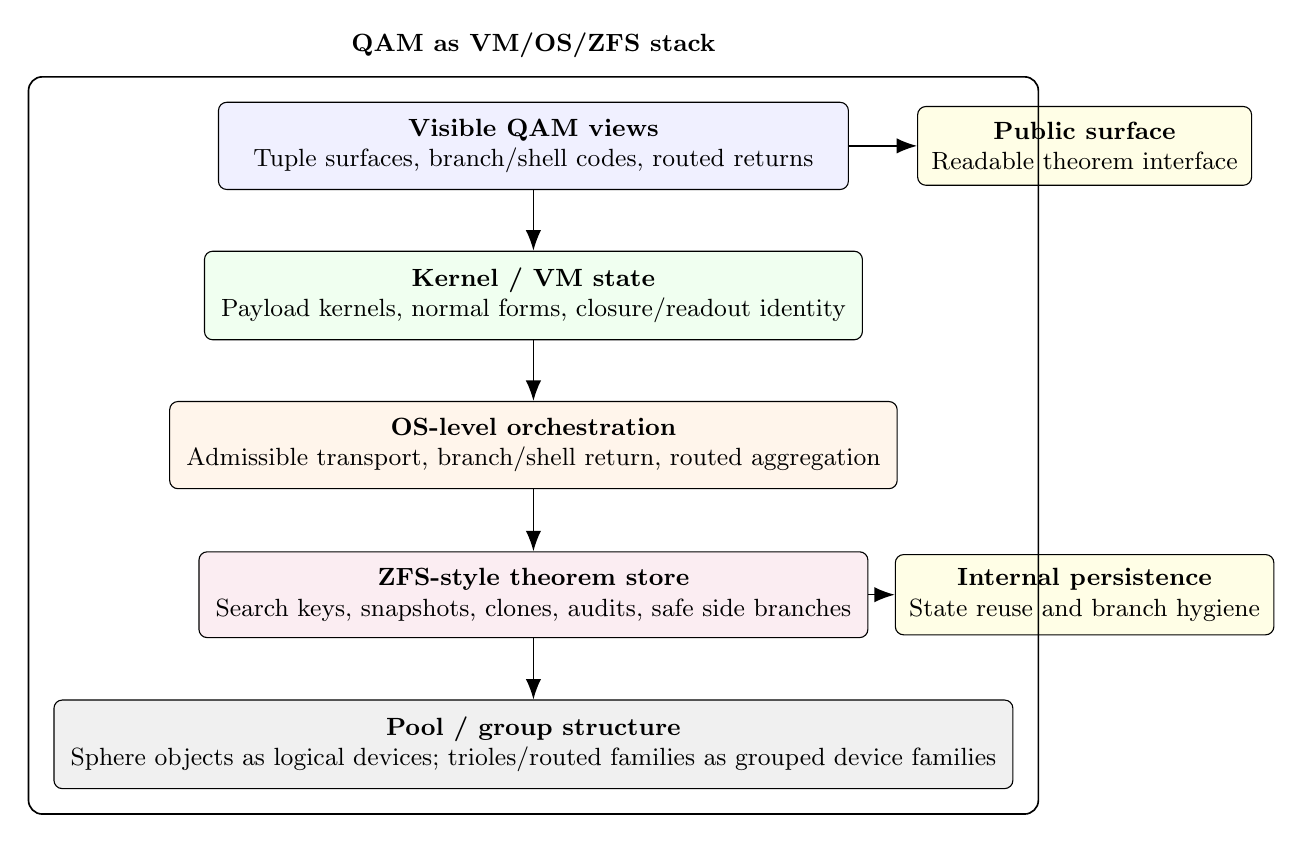
\begin{tikzpicture}[
  font=\small,
  mainbox/.style={draw, rounded corners=3pt, align=center, minimum width=8.0cm, minimum height=1.05cm, inner sep=6pt},
  sidebox/.style={draw, rounded corners=3pt, align=center, minimum width=3.9cm, minimum height=1.0cm, inner sep=5pt},
  arr/.style={-{Latex[length=2.6mm]}, line width=0.5pt}
]

\node[mainbox, fill=blue!6]   (visible)  at (0,0)   {\textbf{Visible QAM views}\\Tuple surfaces, branch/shell codes, routed returns};
\node[sidebox, fill=yellow!10] (public)   at (7.0,0)   {\textbf{Public surface}\\Readable theorem interface};
\node[mainbox, fill=green!6]  (kernel)   at (0,-1.9) {\textbf{Kernel / VM state}\\Payload kernels, normal forms, closure/readout identity};
\node[mainbox, fill=orange!8] (os)       at (0,-3.8) {\textbf{OS-level orchestration}\\Admissible transport, branch/shell return, routed aggregation};
\node[mainbox, fill=purple!7] (store)    at (0,-5.7) {\textbf{ZFS-style theorem store}\\Search keys, snapshots, clones, audits, safe side branches};
\node[sidebox, fill=yellow!10] (internal) at (7.0,-5.7) {\textbf{Internal persistence}\\State reuse and branch hygiene};
\node[mainbox, fill=gray!12]  (pool)     at (0,-7.6) {\textbf{Pool / group structure}\\Sphere objects as logical devices; trioles/routed families as grouped device families};

\draw[arr] (visible) -- (kernel);
\draw[arr] (kernel) -- (os);
\draw[arr] (os) -- (store);
\draw[arr] (store) -- (pool);
\draw[arr] (visible.east) -- (public.west);
\draw[arr] (store.east) -- (internal.west);

\node[draw, rounded corners=5pt, fit=(visible)(kernel)(os)(store)(pool), inner sep=9pt, line width=0.6pt] (stackfit) {};
\node[above=0.15cm of stackfit.north, fill=white, inner sep=2pt] {\textbf{QAM as VM/OS/ZFS stack}};
\end{tikzpicture}%
}\caption{Graphical reading of the current QAM export as a virtual-machine/OS stack with a ZFS-style structural store. Visible tuple surfaces provide the public theorem interface; exposed payload kernels and kernel normal forms provide the later machine-state identity; snapshots, clones, search keys, and audits manage the internal proof store without changing the visible public QAM syntax.}
\label{fig:qam-vm-os-zfs}
\end{figure}

\begin{remark}[Why the ZFS analogy is structurally useful here]\label{rem:qam-zfs-utility}
The ZFS-style reading is not meant as decorative metaphor. It isolates four practical gains already visible in the present file. First, equal kernel classes can later be treated as mirror-like state reuse rather than as repeatedly independent visible tuple surfaces. Second, the deferred kernel-first path already behaves like copy-on-write: experimental compression statements are developed beside the active tuple proofs without rewriting the active line. Third, checkpoints, audits, and activation criteria behave like snapshots and scrub rules for the theorem store, since they record exactly which deferred branches are stable and which still remain non-authoritative. Fourth, once kernel normal forms and search keys are in place, repeated branch/shell/routed return families can be indexed and deduplicated as one structural graph beneath a readable tree-shaped theorem presentation. This is precisely why the systems analogy deserves a more prominent place next to the public QAM extraction itself.
\end{remark}

\begin{remark}[Current scope of the VM/OS/ZFS view]\label{rem:qam-vm-os-scope}
In v3.16.0 this systems view remains explanatory and organizational. It does not introduce a second formal semantics, and it does not yet activate RAID-like reconstruction as an active theorem rule. The present mathematically justified gains are the mirror-like reuse of equal kernel classes, the snapshot/clone logic of active versus deferred proof branches, and the content-addressed search-key discipline attached to kernel normal forms. Stronger pool/reconstruction language should remain subordinate to those already visible gains until the kernel-first activation package has been discharged on the active QAM surface.
\end{remark}


\begin{remark}[How the systems view reads the present visual diagnostics]\label{rem:qam-vm-os-visuals}
The same stack view also explains why Appendix~C may carry highly visible packet, Julia-boundary, and frame-flicker diagnostics without turning those figures into primary closure axioms. In the systems reading, such figures live on the visible-view layer: they are auditable readout surfaces of one and the same transported channel, not independent kernel identities. This is exactly why the OP~5 packet/breathing/frame-flicker block and the Julia-boundary block belong naturally to the same document architecture as the deferred kernel store. The figures make visible what the current theorem store is tracking, while closure itself still remains controlled at the structural layer beneath the pictures.
\end{remark}


\begin{remark}[QAM/systems crosswalk for the present document]\label{rem:qam-vm-os-crosswalk}
The present document uses the systems analogy in a disciplined layer-by-layer way. The following crosswalk fixes the intended reading.
\begin{center}
\renewcommand{\arraystretch}{1.12}
\begin{tabular}{|p{0.29\textwidth}|p{0.28\textwidth}|p{0.31\textwidth}|}
\hline
\textbf{QAM/document layer} & \textbf{Systems reading} & \textbf{Present mathematical status} \\
\hline
Visible coded tuples, packet diagnostics, Julia views, routed return surfaces & User-facing VM/view layer & Actively visible and auditable, but not by themselves closure-generating \\
\hline
Exposed payload kernels and later zero-kernel re-readings & VM-state identity layer & Deferred and prospective only; not yet activated on the public tuple surface \\
\hline
Admissible transport, branch/shell return, routed support organization & OS-level orchestration layer & Active theorem content in the present QAM export \\
\hline
Kernel normal forms, search keys, snapshots, clones, audits & ZFS-style theorem-store layer & Partly active as organizational discipline, partly deferred as later compression infrastructure \\
\hline
Pool/group structure of sphere objects and support families & Device / vdev / pool layer & Explanatory architecture only at the present stage \\
\hline
\end{tabular}
\end{center}
\end{remark}

\begin{remark}[Visual-evidence discipline under the systems reading]\label{rem:qam-vm-os-visual-discipline}
Under the crosswalk above, a figure may support only a controlled class of claims. It may expose \emph{where} a visible readout departs from a rigid carrier picture, \emph{which} packet or channel decomposition is plausible on the view layer, and \emph{why} a later kernel-first compression path is worth isolating. It may \emph{not} by itself create a new closure axiom, replace an active transport/branch/shell/routed theorem, or identify a kernel class solely from appearance. Any later proof use must therefore pass through the active theorem layer or through a deferred bridge that has itself already been discharged.
\end{remark}


\noindent\textbf{v3.16.0 checkpoint (deferred kernel-first path).} The deferred kernel-first material added in the present local v3.16.0 line should be read as one controlled checkpoint rather than as a second public language block. Its current role is to prepare a later proof-compression path while leaving the active coded tuple predicates unchanged.

\begin{remark}[Checkpoint summary for the deferred kernel-first path in the v3.16.0 public release]\label{rem:qam-zero-kernel-checkpoint}
At the present stage, the deferred kernel-first path contributes six concrete pieces of structure.
\begin{enumerate}[leftmargin=2em]
  \item It introduces a prospective recursive zero-kernel vocabulary in which the visible state surface $\langle 0,a\rangle$ may later be re-read through exposed payload kernels, kernel normal forms, and class-level readout factorization.
  \item It records a normal-form and search-key discipline so that later graph/tree based proof search can be tied to canonical kernel representatives rather than to repeated visible tuple surfaces.
  \item It isolates the missing bridge datum from active state surfaces to canonical kernels and identifies the direct visible payload as the simplest current kernel candidate on the present tuple surface.
  \item It tests the resulting kernel-first viewpoint on the three most relevant compression stages of the current QAM line: admissible transport, local branch-shell return, and routed family compression.
  \item It formulates an explicit activation package and a staged migration roadmap, making clear both what would have to be proved before activation and in which order the relevant closure/readout factorization work should be completed.
  \item It remains strictly deferred: no active public predicate, closure theorem, transport theorem, branch-shell theorem, routed-support theorem, or translation theorem is replaced by the kernel language at the present stage.
\end{enumerate}
\end{remark}

\begin{remark}[Why this checkpoint matters for later proof compression]\label{rem:qam-zero-kernel-checkpoint-why}
The checkpoint above already shows where later proof compression would come from. Transport is the first chain-level reduction, branch-shell return the first local surface reduction, routed support the first family reduction, and the translation theorem then becomes the first clause-level reduction at theorem scale. This does not yet shorten the active proofs automatically, but it isolates a concrete path by which set-theoretic comparison load could later be shifted from repeated visible tuple surfaces to kernel normal forms and one final class-level readout step.
\end{remark}

\begin{remark}[Navigation guide for the deferred kernel-first checkpoint]\label{rem:qam-zero-kernel-navigation}
A reader who wants the shortest route through the deferred material may follow the following order.
\begin{enumerate}[leftmargin=2em]
  \item \textbf{Purpose and fit.} Start with the roadmap-fit remark, the checkpoint summary, and the companion remark on why the checkpoint matters in order to see why the deferred path belongs to the inherited public-shape v3.16.0 release layer without changing the public branch/shell/routed extraction.
  \item \textbf{Vocabulary.} Then read the terminological convention for the deferred kernel path together with Definitions~\ref{def:qam-zero-kernel}--\ref{def:qam-kernel-key} for the later kernel vocabulary, primitive zero-objects, recursive reuse, aspect projections, normal forms, and internal search keys.
  \item \textbf{Compatibility.} Next read the axiom-coherence audit together with the current-limitation remark to see why this vocabulary remains deferred and does not compete with the active tuple layer.
  \item \textbf{Bridge.} Then read Definition~\ref{def:qam-kernel-bridge-datum}, Theorem~\ref{thm:qam-kernel-bridge}, Definition~\ref{def:qam-visible-payload}, and Theorem~\ref{thm:qam-direct-kernel-constructor} for the exact interface between visible state surfaces and later kernel-first comparison.
  \item \textbf{Stress tests.} Only afterwards read Propositions~\ref{prop:qam-kernel-first-transport}, \ref{prop:qam-kernel-first-branch-shell}, and \ref{prop:qam-kernel-first-routed}, which test the bridge on transport, local return, and routed family compression.
  \item \textbf{Activation and use.} Finally read Definition~\ref{def:qam-zero-kernel-activation-package}, Theorem~\ref{thm:qam-zero-kernel-activation-criterion}, the later activation-roadmap and reading-guide remarks, and then the dependency-map, minimal-proof-obligation, local-admissibility, and rewrite-schema remarks for the activation threshold, staged migration order, dependency logic, and later local rewrite test.
\end{enumerate}
In that order, the deferred block reads as one controlled proof-compression path rather than as a loose collection of auxiliary notes.
\end{remark}

\begin{remark}[Execution rule for the deferred kernel-first path]\label{rem:qam-zero-kernel-execution-rule}
The deferred block should be used in only one direction when later proof compression is attempted on the present tuple surface. Start with the visible state surface, expose the payload kernel, pass to kernel normal form, prove closure or readout agreement at class level, and lift back to the visible surface only at the end. If the later local admissibility test fails at any point, then the argument should remain on the active tuple surface rather than forcing a premature kernel-first rewrite.
\end{remark}

\begin{remark}[Present-use restriction for the deferred kernel-first path]\label{rem:qam-zero-kernel-present-use}
Until the activation criterion of Theorem~\ref{thm:qam-zero-kernel-activation-criterion} has been fully discharged on the current QAM surface, the deferred block should be used in only three ways inside the document: as later migration vocabulary, as an audit of where proof compression could occur, and as a record of staged stress tests. It should not be cited as a replacement for any active tuple predicate, transport theorem, branch-shell theorem, routed-support theorem, or translation theorem. In particular, whenever both a visible-surface proof and a deferred kernel-first restatement are available, the visible-surface proof remains authoritative on the inherited public-shape v3.16.0 layer.
\end{remark}


\begin{remark}[Active/deferred correspondence rule]\label{rem:qam-zero-kernel-correspondence}
The deferred kernel-first path may also be read as a controlled shadow of four active theorem layers, with one fixed discipline: the active visible-surface theorem remains authoritative, while the deferred statement records only the later compression route attached to that theorem. Concretely, Theorem~\ref{thm:qam-first-op-transport} is paired with Proposition~\ref{prop:qam-kernel-first-transport} as the chain-level compression test; Theorem~\ref{thm:qam-branch-shell} is paired with Proposition~\ref{prop:qam-kernel-first-branch-shell} as the local return-surface compression test; Theorem~\ref{thm:qam-routed-support} is paired with Proposition~\ref{prop:qam-kernel-first-routed} as the family-level compression test; and Theorem~\ref{thm:qam-translation} is paired with the later local admissibility reading of the translation theorem as the clause-level compression test. This correspondence is only a reading rule for later migration work. It does not transfer proof authority from the active theorem to its deferred companion; it only says where a later kernel-first rewrite would have to pay off if the activation package were eventually discharged.
\end{remark}

\subsection*{Prospective recursive zero-kernel scheme (deferred architecture note)}

The following block records a possible later re-reading of the current $\langle 0,a\rangle$-entry as a recursive order-$0$ readout kernel. It is included here only as a controlled design note for future transfer work. It is \emph{not} activated as part of the present public QAM tag system and does not modify the inherited public-shape coded predicates from v3.16.0.

\begin{remark}[Terminological convention for the deferred kernel path]\label{rem:qam-zero-kernel-terminology}
Throughout the deferred block, four layers should be kept distinct and named consistently. The expression \emph{visible state surface} refers to the active public state-code presentation $s=\langle 0,a\rangle$ on the current tuple level. The expression \emph{exposed payload kernel} refers to the payload extracted from such a visible state surface by the deferred kernel constructor. The expression \emph{kernel normal form} refers to the canonical representative selected from the admissible kernel equivalence class. Finally, \emph{class-level readout factorization} means that closure-relevant readout depends only on that kernel normal-form class and is lifted back to the visible state surface only at the end. This convention is purely terminological, but it keeps the active tuple language and the deferred kernel language aligned.
\end{remark}

\begin{definition}[Carrier/filter readout kernels]\label{def:qam-zero-kernel}
Let $\mathcal C$ be a class of admissible carriers, let $\Gamma$ be a class of admissible filters, and let $\mathcal A$ be a class of canonical readout kernels. For each $\gamma\in\Gamma$, assume a partial readout map
\[
\rho_\gamma:\mathcal C \dashrightarrow \mathcal A,
\]
whose defined values are written
\[
a=\rho_\gamma(T)\in\mathcal A.
\]
We read $a$ as the minimal canonical readout kernel of the carrier $T$ relative to the filter $\gamma$.
\end{definition}

\begin{definition}[Primitive zero-objects]\label{def:qam-zero-objects}
Given $a,b\in\mathcal A$, define the primitive zero-objects
\[
Z_0(a):=\langle 0,a\rangle,
\qquad
Z_0(a,b):=\langle 0,a,b\rangle.
\]
The intended reading is that $Z_0(a)$ is the unary collapsed readout attached to the kernel $a$, while $Z_0(a,b)$ is the binary collapsed readout attached to the kernel pair $(a,b)$.
\end{definition}

\begin{axiom}[Recursive reusability of kernels]\label{ax:qam-zero-recursive}
Every canonical readout kernel may again serve as an effective carrier for further admissible readout. Concretely, for admissible $\eta\in\Gamma$, one may again form
\[
\rho_\eta(a)\in\mathcal A
\]
whenever the corresponding readout is defined. Thus the kernel class $\mathcal A$ is recursively reusable as an effective carrier layer.
\end{axiom}

\begin{definition}[Aspect projections on kernels]\label{def:qam-kernel-aspects}
Assume that each kernel $a\in\mathcal A$ comes equipped with aspect projections
\[
\pi_{\mathrm{type}}(a),\qquad
\pi_{\mathrm{class}}(a),\qquad
\pi_{\mathrm{sig}}(a),
\]
recording, respectively, its visible type aspect, filter/class aspect, and structured signature aspect. These are not treated as three competing objects; they are three admissible readings of the same kernel.
\end{definition}

\begin{lemma}[Unary and binary kernel collapse]\label{lem:qam-zero-collapse}
If $a=\rho_\gamma(T)\in\mathcal A$, then the unary zero-object $Z_0(a)=\langle 0,a\rangle$ is well-defined. If additionally $b=\rho_\eta(U)\in\mathcal A$, then the binary zero-object $Z_0(a,b)=\langle 0,a,b\rangle$ is well-defined.
\end{lemma}

\begin{proof}
The unary claim follows directly from Definition~\ref{def:qam-zero-objects} once $a\in\mathcal A$ is given by Definition~\ref{def:qam-zero-kernel}. The binary claim is identical after adjoining a second admissible kernel $b\in\mathcal A$.
\end{proof}

\begin{remark}[Compressed relation to the current $\langle 0,a\rangle$ state code]\label{rem:qam-zero-compressed}
This deferred kernel notation is intended only as a future re-reading of the present visible state surface. In a later binary-tag or order-sensitive QAM line, one may reinterpret the current $\langle 0,a\rangle$ notation as a compressed public surface for a filtered order-$0$ readout kernel. For the present version, however, the active public predicates remain exactly those of the current tagged tuple language.
\end{remark}

\begin{remark}[Tree/graph viewpoint for recursive kernels]\label{rem:qam-zero-graph}
The recursive kernel picture admits an immediate combinatorial visualization. One may regard repeated kernel readout
\[
T \xrightarrow{\rho_\gamma} a \xrightarrow{\rho_\eta} a' \xrightarrow{\rho_\theta} a''
\]
as a rooted readout tree whose vertices are kernels and whose edges are admissible filter applications. Equally, one may organize the same data as a directed multigraph: unary zero-objects $Z_0(a)$ mark collapsed kernel vertices, while binary zero-objects $Z_0(a,b)$ record elementary visible relations between kernel vertices. This suggests a later graph-based search or proof-compression interface without changing the current public tuple system.
\end{remark}


\subsection*{Prospective kernel normal forms and search keys (deferred architecture note)}

The same deferred kernel language also suggests a later search discipline in which recursive kernel proofs are first normalized and only then indexed. This block is likewise prospective only: it does not alter the active inherited public-shape tuple predicates.

\begin{definition}[Kernel equivalence and canonical normal form]\label{def:qam-kernel-normal-form}
Assume an admissible equivalence relation $\sim$ on $\mathcal A$ such that equivalent kernels have the same admissible aspect projections and the same closure-relevant readout content. A \emph{kernel normal form} is a partial map
\[
\operatorname{nf}:\mathcal A \dashrightarrow \mathcal A
\]
selecting, whenever defined, one canonical representative from each admissible equivalence class. Thus
\[
a\sim b \Longrightarrow \operatorname{nf}(a)=\operatorname{nf}(b)
\]
whenever both normal forms are defined.
\end{definition}

\begin{definition}[Kernel search keys]\label{def:qam-kernel-key}
Assume a fixed admissible serialization
\[
\operatorname{ser}:\operatorname{nf}(\mathcal A)\to \Sigma^*
\]
of canonical kernels into finite strings over an alphabet $\Sigma$, together with a deterministic key map
\[
\kappa := H\circ \operatorname{ser}\circ \operatorname{nf}.
\]
The value $\kappa(a)$ is called the \emph{kernel search key} of $a$ whenever the normal form is defined. It is intended as an internal search/index key rather than as part of the visible mathematical surface.
\end{definition}

\begin{lemma}[Normal-form invariance of primitive zero-objects]\label{lem:qam-zero-normal-form}
Assume that $a,a',b,b'\in\mathcal A$ satisfy $a\sim a'$ and $b\sim b'$, and that their normal forms are defined. Then the unary zero-objects $Z_0(a)$ and $Z_0(a')$ determine the same canonical unary kernel surface, while the binary zero-objects $Z_0(a,b)$ and $Z_0(a',b')$ determine the same canonical binary kernel surface after passage to kernel normal form.
\end{lemma}

\begin{proof}
By Definition~\ref{def:qam-kernel-normal-form}, equivalence implies equality of canonical normal forms. Applying the same normal-form representative at the unary or binary zero-object level yields the same canonical collapsed surface in either case.
\end{proof}

\begin{remark}[Graph search and proof-compression interface]\label{rem:qam-kernel-search}
In the graph viewpoint introduced above, one may therefore index vertices by canonical kernel normal forms or, internally, by their kernel search keys $\kappa(a)$. Repeated readout branches that land in the same canonical kernel class can then be merged, memoized, or searched only once. This is exactly the kind of mechanism by which recursive kernel language could later compress set-theoretic proof search without changing the visible public theorem statements.
\end{remark}


\subsection*{Axiom-coherence audit and prospective proof reductions (deferred audit note)}

The deferred zero-kernel language should be read together with the active public QAM tuple layer under the following discipline.

\begin{remark}[Axiom-coherence audit]\label{rem:qam-zero-axiom-audit}
At the present stage, the deferred zero-kernel layer is formally compatible with the active QAM tuple layer for four reasons.
\begin{enumerate}
\item The active tuple predicates remain unchanged: in particular,
\[
\mathrm{QState}(x)\Longleftrightarrow \exists a\,(x=\langle 0,a\rangle)
\]
continues to define the public visible state surface.
\item The deferred zero-kernel definitions do not introduce a second active state predicate. They only record a possible later re-reading of the same public surface, as stated in Remark~\ref{rem:qam-zero-compressed}.
\item The recursive kernel axiom (Axiom~\ref{ax:qam-zero-recursive}) and the kernel normal-form discipline (Definition~\ref{def:qam-kernel-normal-form}) are prospective only; no active theorem in the inherited public-shape QAM chain depends on them as hypotheses.
\item Consequently, the current closure-class, admissible-transport, branch/shell, routed-support, and translation theorems remain exactly those of the active tuple language. The deferred kernel layer adds a controlled future interpretation, not a rival public axiom system.
\end{enumerate}
\end{remark}

\begin{remark}[Where kernel notation could already shorten proofs]\label{rem:qam-zero-proof-opportunities}
Even before formal activation, the deferred kernel language already points to three concrete proof-compression opportunities.
\begin{enumerate}
\item In the first QAM transport theorem, the chain
\[
s_{\mathrm{in}},\ s_2,\ s_3,\ s_4,\ t_{\mathrm{fwd}},\ t_{\mathrm{bwd}}
\]
is currently carried at full state-code level. A later kernel reduction could first pass each state to a canonical readout kernel and then prove closure agreement on kernel classes before lifting the result back to coded states.
\item In the branch-shell theorem and the routed admissible support theorem, each return realization currently enters through full branch/shell state data. A kernel-first restatement could instead reduce every admissible branch-shell realization to unary kernel surfaces $Z_0(a)$ and compare routed sectors only through their canonical kernel classes.
\item In closure-compatible readout arguments, one currently factors raw readouts through the class-target map $J$ after proving $\mathrm{QClEq}(s,t)$. A later kernel language could absorb much of this step by treating the closure-relevant image itself as the primitive kernel surface attached to the state.
\end{enumerate}
In all three cases, the expected gain is not a new theorem but a shorter proof path: reduce to kernels first, perform the closure comparison there, and only then return to the visible tuple layer.
\end{remark}

\begin{remark}[Current limitation of the kernel reduction]\label{rem:qam-zero-current-limit}
The proof-compression opportunities recorded just above are not yet activated as a formal replacement inside the present proofs. The missing step is a theorem-level bridge showing that every active coded state relevant to the admissible OP fragment carries a canonical kernel representative with the same closure-relevant content. Until such a bridge is proved, the zero-kernel language should be treated as a planning interface rather than as a proof rule.
\end{remark}



\begin{definition}[Prospective kernel bridge datum on active state surfaces]\label{def:qam-kernel-bridge-datum}
A \emph{kernel bridge datum} for the active admissible OP fragment consists of a partial map
\[
\operatorname{ker}:\mathcal S^{\mathrm{QAM}}_{\mathrm{act}} \dashrightarrow \mathcal A,
\]
where $\mathcal S^{\mathrm{QAM}}_{\mathrm{act}}$ is the class of active coded QAM-state surfaces relevant to the present admissible OP fragment, such that the following hold whenever the displayed expressions are defined.
\begin{enumerate}
\item \textbf{surface realization:}
\[
Z_0(\operatorname{ker}(s))=s;
\]
\item \textbf{closure reflection:} if $\mathrm{QClEq}(s,t)$, then
\[
\operatorname{nf}(\operatorname{ker}(s))=\operatorname{nf}(\operatorname{ker}(t));
\]
\item \textbf{closure-readout factorization:} for every closure-compatible coded readout $r$, there exists a map
\[
\mathcal R_r: \operatorname{nf}(\mathcal A) \to \operatorname{Im}(J_r)
\]
into the closure-relevant target of the associated class-factor map $J_r$ such that whenever $\mathrm{QRead}(r,s,w)$ holds,
\[
J_r(w)=\mathcal R_r(\operatorname{nf}(\operatorname{ker}(s))).
\]
\end{enumerate}
\end{definition}

\begin{theorem}[Prospective bridge from active state surfaces to canonical kernels]\label{thm:qam-kernel-bridge}
Assume a kernel bridge datum in the sense of Definition~\ref{def:qam-kernel-bridge-datum}. Then every active closure comparison in the admissible OP fragment may be reduced to canonical kernel comparison before returning to the visible state surface. In particular:
\begin{enumerate}
\item if $\mathrm{QAdmTransport}(o,s,t)$, then
\[
\operatorname{nf}(\operatorname{ker}(s))=\operatorname{nf}(\operatorname{ker}(t));
\]
\item if $t_{b,\sigma}$ is a branch-shell coded return realization as in Theorem~\ref{thm:qam-branch-shell}, then
\[
\operatorname{nf}(\operatorname{ker}(s_{\mathrm{in}}))=\operatorname{nf}(\operatorname{ker}(t_{b,\sigma}));
\]
\item if $u$ is a normalized admissible routed support code as in Theorem~\ref{thm:qam-routed-support}, then for every closure-compatible coded readout $r$ the closure-relevant image of the routed return is determined solely by the canonical kernel class
\[
\operatorname{nf}(\operatorname{ker}(s_{\mathrm{in}})).
\]
\end{enumerate}
Consequently, the present transport, branch/shell, and routed-support proofs admit a future kernel-first proof skeleton: first pass to $\operatorname{nf}(\operatorname{ker}(\cdot))$, then compare closure there, and only afterwards return to the visible QAM state surface.
\end{theorem}

\begin{proof}
For (1), admissible transport implies $\mathrm{QClEq}(s,t)$ by the active closure-preservation axiom. The closure-reflection clause of Definition~\ref{def:qam-kernel-bridge-datum} therefore yields
\[
\operatorname{nf}(\operatorname{ker}(s))=\operatorname{nf}(\operatorname{ker}(t)).
\]
For (2), Theorem~\ref{thm:qam-branch-shell} gives $\mathrm{QClEq}(s_{\mathrm{in}},t_{b,\sigma})$, so the same closure-reflection clause yields equality of canonical kernel representatives. For (3), Theorem~\ref{thm:qam-routed-support} states that the routed return has the same closure-relevant image as the coded source state under every closure-compatible coded readout. By clause (3) of Definition~\ref{def:qam-kernel-bridge-datum}, those closure-relevant images factor through the same canonical kernel normal form. Hence the routed readout depends only on $\operatorname{nf}(\operatorname{ker}(s_{\mathrm{in}}))$. The final sentence is simply the proof reading order extracted from (1)--(3).
\end{proof}

\begin{remark}[What the bridge theorem still leaves open]\label{rem:qam-kernel-bridge-open}
Theorem~\ref{thm:qam-kernel-bridge} is intentionally conditional. It does not yet prove that a kernel bridge datum exists inside the active public tuple system; it isolates exactly the missing interface that would be needed to turn the deferred zero-kernel language into an actual proof tool. This also identifies the next genuine activation step: construct $\operatorname{ker}$ canonically from active coded states and verify clauses (1)--(3) without leaving the current OP/QAM semantics.
\end{remark}


\begin{definition}[Visible payload extraction on active state surfaces]\label{def:qam-visible-payload}
For every active coded state surface $s$ in the present public tuple language, define its \emph{exposed payload kernel} $\operatorname{vp}(s)$ by
\[
\operatorname{vp}(s)=a \quad\Longleftrightarrow\quad s=\langle 0,a\rangle.
\]
Equivalently, $\operatorname{vp}$ is the unique projection that removes the visible state tag $0$ and exposes the payload already carried by the active state surface.
\end{definition}

\begin{definition}[Prospective direct kernel constructor]\label{def:qam-direct-kernel-constructor}
Assume that the exposed payload kernel of every active coded state surface relevant to the admissible OP fragment belongs to the deferred kernel class $\mathcal A$. Then define the \emph{direct kernel constructor}
\[
\operatorname{ker}_{\mathrm{dir}} : \mathcal S^{\mathrm{QAM}}_{\mathrm{act}} \dashrightarrow \mathcal A,
\qquad
\operatorname{ker}_{\mathrm{dir}}(s):=\operatorname{vp}(s).
\]
Thus, on the visible state surface, the simplest possible kernel candidate is obtained by forgetting only the active state tag and keeping the payload itself as the deferred kernel representative.
\end{definition}

\begin{theorem}[Simplest concrete kernel construction on the present state surface]\label{thm:qam-direct-kernel-constructor}
Assume the following four conditions for the active admissible OP fragment.
\begin{enumerate}
\item \textbf{payload admissibility:} every active coded state surface $s$ relevant to the fragment has the form $s=\langle 0,a\rangle$ with $a\in\mathcal A$;
\item \textbf{visible zero-surface realization:} for every such $a$,
\[
Z_0(a)=\langle 0,a\rangle;
\]
\item \textbf{closure reflection on exposed payload kernels:} whenever $\mathrm{QClEq}(\langle 0,a\rangle,\langle 0,b\rangle)$,
\[
\operatorname{nf}(a)=\operatorname{nf}(b);
\]
\item \textbf{class-level readout factorization:} for every closure-compatible coded readout $r$, there exists a map
\[
\widetilde{\mathcal R}_r:\operatorname{nf}(\mathcal A)\to \operatorname{Im}(J_r)
\]
such that whenever $\mathrm{QRead}(r,\langle 0,a\rangle,w)$,
\[
J_r(w)=\widetilde{\mathcal R}_r(\operatorname{nf}(a)).
\]
\end{enumerate}
Then $\operatorname{ker}_{\mathrm{dir}}$ is a kernel bridge datum in the sense of Definition~\ref{def:qam-kernel-bridge-datum}. Consequently Theorem~\ref{thm:qam-kernel-bridge} applies with
\[
\operatorname{ker}=\operatorname{ker}_{\mathrm{dir}}.
\]
\end{theorem}

\begin{proof}
Clause (1) ensures that $\operatorname{ker}_{\mathrm{dir}}$ is defined on every active state surface relevant to the fragment. By Definition~\ref{def:qam-visible-payload}, if $s=\langle 0,a\rangle$, then $\operatorname{ker}_{\mathrm{dir}}(s)=a$. Clause (2) therefore gives
\[
Z_0(\operatorname{ker}_{\mathrm{dir}}(s))=Z_0(a)=\langle 0,a\rangle=s,
\]
which is exactly the surface-realization clause of Definition~\ref{def:qam-kernel-bridge-datum}. For closure reflection, if $\mathrm{QClEq}(s,t)$ with $s=\langle 0,a\rangle$ and $t=\langle 0,b\rangle$, clause (3) gives
\[
\operatorname{nf}(\operatorname{ker}_{\mathrm{dir}}(s))=\operatorname{nf}(a)=\operatorname{nf}(b)=\operatorname{nf}(\operatorname{ker}_{\mathrm{dir}}(t)).
\]
Finally, clause (4) is exactly the required closure-readout factorization after substituting $\operatorname{ker}_{\mathrm{dir}}(\langle 0,a\rangle)=a$. Hence all three clauses of Definition~\ref{def:qam-kernel-bridge-datum} hold.
\end{proof}

\begin{remark}[What this construction shows]\label{rem:qam-direct-kernel-constructor-meaning}
Theorem~\ref{thm:qam-direct-kernel-constructor} shows that the difficult part of the bridge is not the extraction step itself: on the current public state surface, the most economical candidate is simply the exposed payload of the active state surface. The real work is pushed into the three semantic checks: that the payload already lies in the admissible kernel class, that closure equivalence is visible at payload-normal-form level, and that closure-relevant readout factors through that same normal form. If these three checks can later be discharged, then many current state-level proofs may be shortened by passing immediately from $\langle 0,a\rangle$ to $a$ before performing the closure comparison.
\end{remark}

\subsection*{QAM minimal predicates and coded relations}

We now pass from the entry-layer preview to the first explicit predicate layer of QAM-over-ZF. At this stage, the QAM language still remains conservative over ZF: the predicates below are intended as definable recognition or relation clauses on tagged set-codes rather than as commitments to a new ontology.

\begin{definition}[Primitive QAM predicates]
We introduce the primitive predicates
\[
\begin{aligned}
&\mathrm{QState}(x),\quad \mathrm{QLayer}(x),\quad \mathrm{QOp}(x),\quad \mathrm{QReadout}(x),\\[0.15em]
&\mathrm{QBranch}(x),\quad \mathrm{QShell}(x),\quad \mathrm{QWitness}(x),\quad \mathrm{QTensor}(x).
\end{aligned}
\]
with the intended ZF-grounded readings
\[
\mathrm{QState}(x)\;:\Longleftrightarrow\;\exists a\,(x=\langle 0,a\rangle),
\]
\[
\mathrm{QLayer}(x)\;:\Longleftrightarrow\;\exists \ell\,\exists D\,(x=\langle 1,\ell,D\rangle),
\]
\[
\mathrm{QOp}(x)\;:\Longleftrightarrow\;\exists \ell_1\,\exists \ell_2\,\exists G\,(x=\langle 2,\ell_1,\ell_2,G\rangle),
\]
\[
\mathrm{QReadout}(x)\;:\Longleftrightarrow\;\exists \ell\,\exists W\,\exists R\,(x=\langle 3,\ell,W,R\rangle),
\]
\[
\mathrm{QBranch}(x)\;:\Longleftrightarrow\;\exists b\,\exists B\,(x=\langle 4,b,B\rangle),
\]
\[
\mathrm{QShell}(x)\;:\Longleftrightarrow\;\exists r\,\exists s\,\exists T\,(x=\langle 5,r,s,T\rangle),
\]
\[
\mathrm{QWitness}(x)\;:\Longleftrightarrow\;\exists u\,(x=\langle 6,u\rangle),
\]
\[
\mathrm{QTensor}(x)\;:\Longleftrightarrow\;\exists y\,\exists z\,(x=\langle 7,y,z\rangle).
\]
\end{definition}

\begin{remark}
At this stage, these predicates are still recognition clauses rather than a full independent axiom system. Their purpose is to let the Companion speak explicitly about coded states, layers, operators, readouts, branches, shell/refinement objects, witnesses, and tensor composites inside one ZF-grounded language layer.
\end{remark}

\begin{definition}[Primitive QAM coded relations]
We also introduce the primitive QAM-style relations
\[
\mathrm{QAdmTransport}(o,s,t),\qquad
\mathrm{QClEq}(s,t),\qquad
\mathrm{QRead}(r,s,w),
\]
\[
\mathrm{QBranchRef}(b,s,t),\qquad
\mathrm{QShellRef}(\sigma,s,t),\qquad
\mathrm{QTensorAdm}(x,y).
\]
Their intended readings are as follows:
\begin{enumerate}
\item $\mathrm{QAdmTransport}(o,s,t)$ means that the operator-code $o$ transports the coded state $s$ admissibly to the coded state $t$;
\item $\mathrm{QClEq}(s,t)$ means that $s$ and $t$ belong to the same coded closure class;
\item $\mathrm{QRead}(r,s,w)$ means that the readout-code $r$ reads the coded state $s$ into the coded observable value $w$;
\item $\mathrm{QBranchRef}(b,s,t)$ means that the branch-code $b$ refines the coded state $s$ to the coded state $t$;
\item $\mathrm{QShellRef}(\sigma,s,t)$ means that the shell/refinement-code $\sigma$ refines the coded state $s$ to the coded state $t$;
\item $\mathrm{QTensorAdm}(x,y)$ means that the tensor-coded composite $x\otimes y$ is admitted as a legitimate coded QAM object.
\end{enumerate}
\end{definition}

\begin{remark}
These relations are the first minimal bridge between the current OP/branch/shell architecture and its coded QAM-over-ZF form. In particular, admissibility and closure-class preservation already appear here as primitive language-level notions rather than as only informal motivation.
\end{remark}

\begin{definition}[First QAM translation target]
The first intended translation target of the QAM-over-ZF layer is the admissible OP fragment consisting of:
\begin{enumerate}
\item the OP~1/OP~5 source-return closure architecture;
\item the intermediate OP~2--OP~4 transport bridge;
\item admissible branch transport;
\item OP~3 shell-admissible refinement;
\item admissible routed support together with the visible packet/phase-lock/epsilon screening layer.
\end{enumerate}
\end{definition}

\begin{remark}
The significance of the present predicate layer is that QAM is no longer only a roadmap note. Even at this first stage, the language already distinguishes object-kinds and relation-kinds closely enough to serve as a faithful coded entry interface for the current admissible OP fragment.
\end{remark}



\subsection*{QAM transport, closure, and readout schemata}

We now pass from the minimal predicate layer to the first theorematic QAM transport/closure layer. The point of this section is still conservative: it does not yet claim a fully independent QAM foundation, but it does begin to formulate admissible transport, closure-class preservation, and closure-compatible readout directly in the coded QAM-over-ZF language.

\begin{definition}[QAM-coded transport graph]
A QAM-operator code
\[
o=\langle 2,\ell_1,\ell_2,G\rangle
\]
is called a \emph{coded transport graph} if $G$ is a set of ordered pairs coding a functional transport rule from coded states on layer $\ell_1$ to coded states on layer $\ell_2$.
\end{definition}

\begin{definition}[QAM admissible transport]
For a QAM-operator code $o$ and coded states $s,t$, we write
\[
\mathrm{QAdmTransport}(o,s,t)
\]
iff:
\begin{enumerate}
\item $o$ is a coded transport graph;
\item $s$ is a coded state on the source layer of $o$;
\item $t$ is a coded state on the target layer of $o$;
\item the graph-code of $o$ sends $s$ to $t$;
\item the transport from $s$ to $t$ preserves the intended closure-bearing structural mode.
\end{enumerate}
\end{definition}

\begin{remark}
At this stage, the final clause is still schematic. Its precise intended mathematical content is supplied by the coded closure-class relation below.
\end{remark}

\begin{definition}[QAM closure-class equivalence]
The relation
\[
\mathrm{QClEq}(s,t)
\]
is the coded closure-class relation on QAM-state codes. It is intended to mean that $s$ and $t$ represent the same closure-bearing structural mode, even if they differ by admissible transport, admissible frame-shifted realization, admissible branch refinement, or admissible shell refinement.
\end{definition}

\begin{axiom}[QAM closure-class schema]
The relation $\mathrm{QClEq}$ is required to satisfy:
\begin{enumerate}
\item \textbf{reflexivity:}
\[
\mathrm{QClEq}(s,s);
\]
\item \textbf{symmetry:}
\[
\mathrm{QClEq}(s,t)\Longrightarrow \mathrm{QClEq}(t,s);
\]
\item \textbf{transitivity:}
\[
\mathrm{QClEq}(s,t)\wedge \mathrm{QClEq}(t,u)\Longrightarrow \mathrm{QClEq}(s,u).
\]
\end{enumerate}
\end{axiom}

\begin{remark}
Thus $\mathrm{QClEq}$ is the coded QAM analogue of the native closure carrier-class relation used in the current OP architecture.
\end{remark}

\begin{axiom}[QAM admissibility implies closure preservation]
For every operator code $o$ and state codes $s,t$,
\[
\mathrm{QAdmTransport}(o,s,t)\Longrightarrow \mathrm{QClEq}(s,t).
\]
\end{axiom}

\begin{remark}
This is the first central QAM principle. Admissibility is not defined merely by existence of transport, but by preservation of closure class.
\end{remark}

\begin{definition}[QAM-coded readout]
A QAM-readout code
\[
r=\langle 3,\ell,W,R\rangle
\]
is called a \emph{coded readout} if $R$ is a graph-code sending coded states on layer $\ell$ into coded observable values in the target code $W$.
\end{definition}

\begin{definition}[QAM readout relation]
We write
\[
\mathrm{QRead}(r,s,w)
\]
iff $r$ is a coded readout, $s$ is a coded state on the source layer of $r$, and the graph-code of $r$ sends $s$ to the coded observable value $w$.
\end{definition}

\begin{definition}[QAM closure-compatible readout]\label{def:qam-closure-compatible-readout}
A coded readout $r$ is called \emph{closure-compatible} if there exists a coded class-target map $J$ such that for all coded states $s,t$,
\[
\mathrm{QClEq}(s,t)\Longrightarrow
\bigl(
\forall w_1\,\forall w_2\,
(\mathrm{QRead}(r,s,w_1)\wedge \mathrm{QRead}(r,t,w_2)\Longrightarrow J(w_1)=J(w_2))
\bigr).
\]
\end{definition}

\begin{remark}
This is the coded QAM version of readout factorization through closure class. Raw readouts may differ, but their closure-relevant image under $J$ must agree whenever the source states belong to the same closure class.
\end{remark}

\begin{definition}[First tensor-compatibility placeholder]
We reserve the tensor-admissibility predicate
\[
\mathrm{QTensorAdm}(x,y)
\]
for the statement that the tensor-coded composite $x\otimes y$ is admitted as a legitimate coded QAM object of the intended kind.
\end{definition}

\begin{proposition}[First QAM transport principle]
Let $o$ be a coded QAM-operator, let $s,t$ be coded QAM-states, and let $r$ be a closure-compatible coded readout. If
\[
\mathrm{QAdmTransport}(o,s,t),
\]
then:
\begin{enumerate}
\item \[
\mathrm{QClEq}(s,t);
\]
\item the closure-relevant image of any readout of $s$ agrees with the closure-relevant image of any readout of $t$ under the factor map $J$ associated with $r$.
\end{enumerate}
\end{proposition}

\begin{proof}
The first claim is exactly the admissibility-implies-closure-preservation schema. The second follows from closure-compatibility of the readout: since $\mathrm{QClEq}(s,t)$ holds, any coded readouts of $s$ and $t$ are identified after passage through the closure-relevant class-target map $J$.
\end{proof}

\begin{theorem}[First QAM version of the OP transport principle]\label{thm:qam-first-op-transport}
Assume:
\begin{enumerate}
\item there is a coded source state $s_{\mathrm{in}}$;
\item there are coded intermediate states $s_2,s_3,s_4$;
\item there are coded operator maps $o_2,o_3,o_4,o_{\mathrm{fwd}},o_{\mathrm{bwd}}$;
\item the transports
\[
\begin{aligned}
&\mathrm{QAdmTransport}(o_2,s_{\mathrm{in}},s_2),\qquad
\mathrm{QAdmTransport}(o_3,s_2,s_3),\\[0.15em]
&\mathrm{QAdmTransport}(o_4,s_3,s_4),\qquad
\mathrm{QAdmTransport}(o_{\mathrm{fwd}},s_{\mathrm{in}},t_{\mathrm{fwd}}),\\[0.15em]
&\mathrm{QAdmTransport}(o_{\mathrm{bwd}},s_{\mathrm{in}},t_{\mathrm{bwd}}).
\end{aligned}
\]
all hold;
\item the relevant coded readout is closure-compatible.
\end{enumerate}
Then all coded states
\[
s_{\mathrm{in}},\ s_2,\ s_3,\ s_4,\ t_{\mathrm{fwd}},\ t_{\mathrm{bwd}}
\]
belong to the same coded closure class. Consequently, all closure-relevant readouts of these states agree after passage through the closure-factor map.
\end{theorem}

\begin{proof}
Each admissible transport preserves closure class by the admissibility schema. Therefore
\[
\mathrm{QClEq}(s_{\mathrm{in}},s_2),\qquad
\mathrm{QClEq}(s_2,s_3),\qquad
\mathrm{QClEq}(s_3,s_4).
\]
By transitivity,
\[
\mathrm{QClEq}(s_{\mathrm{in}},s_4).
\]
Likewise,
\[
\mathrm{QClEq}(s_{\mathrm{in}},t_{\mathrm{fwd}})
\qquad\text{and}\qquad
\mathrm{QClEq}(s_{\mathrm{in}},t_{\mathrm{bwd}})
\]
follow from admissible forward and backward transport. Using transitivity again, all listed coded states lie in the same closure class. Closure-compatible readout then identifies their closure-relevant readout content after factorization through the associated class-target map.
\end{proof}

\begin{proposition}[Prospective kernel-first reduction of the first transport theorem]\label{prop:qam-kernel-first-transport}
Assume the direct kernel constructor of Definition~\ref{def:qam-direct-kernel-constructor} and the bridge conditions of Theorem~\ref{thm:qam-direct-kernel-constructor}. Write
\[
s_{\mathrm{in}}=\langle 0,a_{\mathrm{in}}\rangle,
\qquad
s_2=\langle 0,a_2\rangle,
\qquad
s_3=\langle 0,a_3\rangle,
\qquad
s_4=\langle 0,a_4\rangle,
\]
\[
t_{\mathrm{fwd}}=\langle 0,a_{\mathrm{fwd}}\rangle,
\qquad
t_{\mathrm{bwd}}=\langle 0,a_{\mathrm{bwd}}\rangle.
\]
Then the conclusion of Theorem~\ref{thm:qam-first-op-transport} may be read kernel-first as follows:
\begin{enumerate}
\item all exposed transport kernels lie in one canonical normal-form class,
\[
\operatorname{nf}(a_{\mathrm{in}})=\operatorname{nf}(a_2)=\operatorname{nf}(a_3)=\operatorname{nf}(a_4)=\operatorname{nf}(a_{\mathrm{fwd}})=\operatorname{nf}(a_{\mathrm{bwd}}),
\]
\item hence every closure-compatible coded readout of the transport chain factors through that single canonical kernel class,
\item therefore the first transport theorem may be re-read as a kernel-normal-form preservation statement along the admissible transport chain before returning to the visible QAM state surface.
\end{enumerate}
\end{proposition}

\begin{proof}
Theorem~\ref{thm:qam-first-op-transport} states that all six visible coded states belong to the same coded closure class. Since each state lies on the present state surface, the direct kernel constructor exposes exactly the exposed payload kernel of each state as its deferred kernel representative. The closure-reflection clause of Theorem~\ref{thm:qam-direct-kernel-constructor} therefore yields equality of the six corresponding kernel normal forms. By the class-level readout factorization clause, every closure-compatible coded readout depends only on that common kernel normal form. Hence the whole transport chain may be treated kernel-first and lifted back to the visible state surface only at the end.
\end{proof}

\begin{remark}[Axiom audit after the kernel-first transport reduction]\label{rem:qam-kernel-first-transport-audit}
Proposition~\ref{prop:qam-kernel-first-transport} does \emph{not} strengthen the active proof status of Theorem~\ref{thm:qam-first-op-transport}. The active theorem still rests only on admissible transport, closure-class preservation, transitivity of coded closure, and closure-compatible coded readout. The kernel-first proposition adds force only under the deferred payload-level bridge hypotheses isolated in Definition~\ref{def:qam-kernel-bridge-datum} and Theorem~\ref{thm:qam-direct-kernel-constructor}. Thus no new hidden axiom has entered the live transport theorem; only a prospective kernel-level compression of its proof surface has been recorded.
\end{remark}

\begin{remark}[How much proof load the kernel-first transport reading removes]\label{rem:qam-kernel-first-transport-savings}
For the present transport theorem the admissible chain contains five explicit transport links:
\[
s_{\mathrm{in}}\to s_2\to s_3\to s_4,
\qquad
s_{\mathrm{in}}\to t_{\mathrm{fwd}},
\qquad
s_{\mathrm{in}}\to t_{\mathrm{bwd}}.
\]
So the gain is again \emph{not} a reduction in the number of transport links, but a reduction in the size of the object carried through each link. On the visible state surface the proof transports closure across five state-surface steps and then factors a closure-compatible readout through the resulting six-state closure class. In the deferred kernel-first reading, those same five links are re-read as five kernel normal-form identifications, followed by one readout through the common kernel class. If one measures a visible-state transport comparison by cost $C_{\mathrm{surf}}$ and a kernel normal-form comparison by cost $C_{\mathrm{ker}}$, then the conceptual load changes from roughly
\[
5\,C_{\mathrm{surf}} + C_{\mathrm{read}}
\]
to
\[
5\,C_{\mathrm{ker}} + C_{\mathrm{class}},
\]
with intended gain $C_{\mathrm{ker}}<C_{\mathrm{surf}}$ and typically $C_{\mathrm{class}}\ll C_{\mathrm{read}}$. So the numerical savings are moderate but already real: the theorem still has five links, yet each link is checked on exposed kernels instead of full visible state surfaces, and the final readout is centralized on one canonical kernel class.
\end{remark}

\begin{remark}
This theorem is only the first coded QAM shadow of the current OP transport architecture. It does not yet include the full branch-shell routed layer, but it already captures the source/intermediate/return logic in a ZF-grounded coded form.
\end{remark}



\subsection*{QAM branch, shell, and routed support layer}

We now extend the QAM-over-ZF language from basic transport and readout to the branch/shell/routed layer. The point of this section is to translate the current admissible-branch, OP~3 shell-admissibility, and admissible routed-support architecture into a single coded QAM fragment without yet claiming a fully independent QAM foundation. For direct continuity with the compact front extraction, the present subsection should be read in the same order as the release dictionary of Remark~\ref{rem:public-shape-reading-guide}: branch admissibility first, shell admissibility second, admissible branch-shell support third, normalized routed support fourth, and only then the visible-versus-structural screening rule.

\begin{definition}[Closure-admissible branch code]
A branch code $b$ is called \emph{closure-admissible} if for all coded states $s,t$,
\[
\mathrm{QBranchRef}(b,s,t)\Longrightarrow \mathrm{QClEq}(s,t).
\]
Equivalently, branch refinement by $b$ preserves the coded closure class.
\end{definition}

\begin{definition}[Shell-admissible refinement code]
A shell/refinement code $\sigma$ is called \emph{shell-admissible} if for all coded states $s,t$,
\[
\mathrm{QShellRef}(\sigma,s,t)\Longrightarrow \mathrm{QClEq}(s,t).
\]
Equivalently, shell-sensitive or residual-sensitive refinement by $\sigma$ preserves the coded closure class.
\end{definition}

\begin{remark}
These are the direct coded QAM analogues of closure-admissible branches and OP~3 shell-admissible refinements in the current Companion line.
\end{remark}

\begin{definition}[Admissible branch set and shell family]
We define the admissible branch class by
\[
\mathcal{B}^{\mathrm{QAM}}_{\mathrm{adm}}
:=
\{\,b:\mathrm{QBranch}(b)\ \wedge\ b\text{ is closure-admissible}\,\},
\]
and for each branch code $b$, the shell-admissible refinement class by
\[
\mathcal{F}^{\mathrm{QAM}}_{\mathrm{sh}}(b)
:=
\{\,\sigma:\mathrm{QShell}(\sigma)\ \wedge\ \sigma\text{ is shell-admissible on }b\,\}.
\]
\end{definition}

\begin{remark}
At this stage, the phrase ``shell-admissible on $b$'' may be read minimally as: shell refinement by $\sigma$ acts on branchwise states associated with $b$ without leaving the coded closure class.
\end{remark}

\begin{definition}[Routed support code]
A \emph{routed support code} is a set-code
\[
u=\langle 8,\Omega,w\rangle,
\]
where $\Omega$ is a coded finite or set-sized support family of admissible branch-shell pairs and $w$ is a coded weight assignment on $\Omega$.
\end{definition}

\begin{definition}[Admissible routed support]
A routed support code
\[
u=\langle 8,\Omega,w\rangle
\]
is called \emph{admissible} if every element of $\Omega$ has the form $(b,\sigma)$ with
\[
b\in \mathcal{B}^{\mathrm{QAM}}_{\mathrm{adm}}
\qquad\text{and}\qquad
\sigma\in \mathcal{F}^{\mathrm{QAM}}_{\mathrm{sh}}(b).
\]
\end{definition}

\begin{remark}
Thus admissible routed support is the coded QAM version of the admissible branch-shell support sector in the current OP architecture.
\end{remark}

\begin{definition}[Normalized routed support]
An admissible routed support code
\[
u=\langle 8,\Omega,w\rangle
\]
is called \emph{normalized} if its coded weight assignment satisfies
\[
\sum_{(b,\sigma)\in\Omega} w(b,\sigma)=1
\]
in the intended decoded numerical target.
\end{definition}

\begin{remark}
The normalization condition is stated semiformally at this stage. In the fully coded version, the sum relation would itself be represented by a suitable arithmetic coding layer over ZF.
\end{remark}

\begin{definition}[Branch-shell coded return realization]
Let $b$ be a closure-admissible branch code and let $\sigma$ be a shell-admissible refinement code on $b$. A \emph{branch-shell coded return realization} is a coded state
\[
t_{b,\sigma}
\]
such that:
\begin{enumerate}
\item $t_{b,\sigma}$ is reached from the coded source state through admissible branch refinement by $b$;
\item the OP~3-level shell refinement by $\sigma$ is shell-admissible;
\item the resulting return-side coded state is read through a closure-compatible coded readout.
\end{enumerate}
\end{definition}

\begin{proposition}[QAM branch admissibility principle]\label{prop:qam-branch-admissibility-principle}
Let $b$ be a closure-admissible branch code. If
\[
\mathrm{QBranchRef}(b,s,t),
\]
then
\[
\mathrm{QClEq}(s,t).
\]
Consequently, every closure-compatible readout identifies the closure-relevant image of $s$ and $t$ after passage through the associated class-factor map.
\end{proposition}

\begin{proof}
The first claim is just the definition of closure-admissibility. The readout claim follows from closure-compatibility of coded readouts: closure-equivalent coded states have the same closure-relevant image after factorization.
\end{proof}

\begin{proposition}[QAM shell admissibility principle]\label{prop:qam-shell-admissibility-principle}
Let $\sigma$ be a shell-admissible refinement code. If
\[
\mathrm{QShellRef}(\sigma,s,t),
\]
then
\[
\mathrm{QClEq}(s,t).
\]
Consequently, shell-sensitive refinement does not alter closure-relevant readout content as long as shell-admissibility is preserved.
\end{proposition}

\begin{proof}
This is the direct content of shell-admissibility together with closure-compatible readout factorization.
\end{proof}

\begin{theorem}[QAM admissible branch-shell theorem]\label{thm:qam-branch-shell}
Let $s_{\mathrm{in}}$ be a coded source state, let $b$ be a closure-admissible branch code, and let $\sigma$ be a shell-admissible refinement code on $b$. Assume there exists a branch-shell coded return realization
\[
t_{b,\sigma}
\]
associated with $(b,\sigma)$, and let $r$ be a closure-compatible coded readout. Then
\[
\mathrm{QClEq}(s_{\mathrm{in}},t_{b,\sigma}).
\]
Hence every closure-compatible readout of $s_{\mathrm{in}}$ and $t_{b,\sigma}$ agrees after passage through its associated closure-factor map.
\end{theorem}

\begin{proof}
By closure-admissibility of $b$, branch refinement preserves the coded closure class. By shell-admissibility of $\sigma$, the shell-sensitive refinement preserves the same coded closure class at the OP~3 layer. Hence the final coded return realization $t_{b,\sigma}$ remains closure-equivalent to the coded source state $s_{\mathrm{in}}$. Closure-compatible readout then identifies the closure-relevant content of both states after factorization.
\end{proof}



\subsection*{Shell certificates and the first OP~3/QAM closure guide}
The next narrow OP~3-oriented extension of the public-shape QAM line is not a broad new tensor layer, but a certificate layer. The goal is to say explicitly when a branch/shell refinement is still the same closure-bearing object, what counts as the first local failure of that claim, and how the deferred kernel bridge should later read that same situation in one compressed normal form. Mixed tensors remain deferred here: they are not introduced unless an actual OP~3 proof step later forces them.

\begin{center}
\fbox{\begin{minipage}{0.93\textwidth}
\small
\textbf{QAM reading key for the OP~3 closure block.}\\[0.2em]
\textbf{Objects:} coded source state $s_{\mathrm{in}}$, closure-admissible branch code $b$, shell refinement code $\sigma$, intermediate branch state $s_b$, branch-shell return state $t_{b,\sigma}$.\\
\textbf{Allowed move:} pass from $s_{\mathrm{in}}$ to $s_b$ by admissible branch refinement and from $s_b$ to $t_{b,\sigma}$ by shell refinement without leaving the closure class.\\
\textbf{Invariant:} the closure-bearing class, and later its kernel/normal-form representative when the deferred bridge is activated.\\
\textbf{Defect signal:} a broken branch clause, a broken shell clause, or a failure of closure-compatible readout factorization.\\
\textbf{Plain-language reading:} OP~3 may change the visible shell, but it must not change the closure-bearing core.
\end{minipage}}
\end{center}

\begin{definition}[Shell admissibility certificate]\label{def:qam-shell-certificate}
Let $s_{\mathrm{in}}$ be a coded source state, let $b$ be a closure-admissible branch code, let $\sigma$ be a shell refinement code, and let $t_{b,\sigma}$ be a branch-shell coded return realization. A \emph{shell admissibility certificate} for $(s_{\mathrm{in}},b,\sigma,t_{b,\sigma})$ consists of coded data witnessing the following four clauses:
\begin{enumerate}[leftmargin=2em]
  \item there exists a coded branch state $s_b$ with $\mathrm{QBranchRef}(b,s_{\mathrm{in}},s_b)$;
  \item the branch code $b$ is closure-admissible;
  \item one has $\mathrm{QShellRef}(\sigma,s_b,t_{b,\sigma})$ and the refinement code $\sigma$ is shell-admissible on $b$;
  \item the return state $t_{b,\sigma}$ is read through a closure-compatible coded readout.
\end{enumerate}
\end{definition}

\begin{definition}[Shell defect witness]\label{def:qam-shell-defect-witness}
A \emph{shell defect witness} for $(s_{\mathrm{in}},b,\sigma,t_{b,\sigma})$ is coded data showing failure of at least one clause of Definition~\ref{def:qam-shell-certificate}. Thus a shell defect witness may record failure of admissible branch passage, failure of shell admissibility, or failure of closure-compatible readout factorization.
\end{definition}

\begin{lemma}[Certificate persistence of closure class]\label{lem:qam-shell-certificate-closure}
Assume that $(s_{\mathrm{in}},b,\sigma,t_{b,\sigma})$ carries a shell admissibility certificate. Then
\[
\mathrm{QClEq}(s_{\mathrm{in}},t_{b,\sigma}).
\]
Hence every closure-compatible coded readout identifies the same closure-relevant image on $s_{\mathrm{in}}$ and $t_{b,\sigma}$ after passage through the associated class-factor map.
\end{lemma}

\begin{proof}
By clause (1) of Definition~\ref{def:qam-shell-certificate}, there exists $s_b$ with
\[
\mathrm{QBranchRef}(b,s_{\mathrm{in}},s_b).
\]
By clause (2), the branch code $b$ is closure-admissible, so Proposition~\ref{prop:qam-branch-admissibility-principle} yields
\[
\mathrm{QClEq}(s_{\mathrm{in}},s_b).
\]
By clause (3), one has
\[
\mathrm{QShellRef}(\sigma,s_b,t_{b,\sigma}),
\]
and the refinement code $\sigma$ is shell-admissible on $b$. Proposition~\ref{prop:qam-shell-admissibility-principle} therefore gives
\[
\mathrm{QClEq}(s_b,t_{b,\sigma}).
\]
Transitivity of the coded closure relation yields
\[
\mathrm{QClEq}(s_{\mathrm{in}},t_{b,\sigma}).
\]
The final sentence is then the usual closure-compatible readout factorization claim.
\end{proof}

\begin{proposition}[Certified kernel persistence for OP~3 shell passage]\label{prop:qam-shell-certificate-kernel}
Assume the direct kernel constructor of Definition~\ref{def:qam-direct-kernel-constructor} and the bridge conditions of Theorem~\ref{thm:qam-direct-kernel-constructor}. Let
\[
s_{\mathrm{in}}=\langle 0,a_{\mathrm{in}}\rangle
\]
be the coded source state, and let
\[
t_{b,\sigma}=\langle 0,a_{b,\sigma}\rangle
\]
be a branch-shell coded return realization. If $(s_{\mathrm{in}},b,\sigma,t_{b,\sigma})$ carries a shell admissibility certificate, then
\[
\operatorname{nf}(a_{b,\sigma})=\operatorname{nf}(a_{\mathrm{in}}).
\]
In particular, certified OP~3 shell passage preserves the kernel normal form of the coded source state.
\end{proposition}

\begin{proof}
By Lemma~\ref{lem:qam-shell-certificate-closure}, one has
\[
\mathrm{QClEq}(s_{\mathrm{in}},t_{b,\sigma}).
\]
The deferred kernel bridge then reflects closure equivalence into equality of canonical kernel normal forms. Since
\[
s_{\mathrm{in}}=\langle 0,a_{\mathrm{in}}\rangle,
\qquad
 t_{b,\sigma}=\langle 0,a_{b,\sigma}\rangle,
\]
this yields
\[
\operatorname{nf}(a_{b,\sigma})=\operatorname{nf}(a_{\mathrm{in}}).
\]
\end{proof}

\begin{theorem}[Shell-stable readout factorization]\label{thm:qam-shell-stable-readout}
Assume the direct kernel constructor of Definition~\ref{def:qam-direct-kernel-constructor} and the bridge conditions of Theorem~\ref{thm:qam-direct-kernel-constructor}. Let
\[
s_{\mathrm{in}}=\langle 0,a_{\mathrm{in}}\rangle,
\qquad
 t_{b,\sigma}=\langle 0,a_{b,\sigma}\rangle,
\]
let $r$ be a closure-compatible coded readout, and assume that $(s_{\mathrm{in}},b,\sigma,t_{b,\sigma})$ carries a shell admissibility certificate. Then for every pair of coded observable values $w_{\mathrm{in}},w_{b,\sigma}$ with
\[
\mathrm{QRead}(r,s_{\mathrm{in}},w_{\mathrm{in}}),
\qquad
\mathrm{QRead}(r,t_{b,\sigma},w_{b,\sigma}),
\]
one has
\[
J_r(w_{\mathrm{in}})
=
\widetilde{\mathcal R}_r(\operatorname{nf}(a_{\mathrm{in}}))
=
\widetilde{\mathcal R}_r(\operatorname{nf}(a_{b,\sigma}))
=
J_r(w_{b,\sigma}).
\]
In particular, every closure-relevant coded readout of a certified OP~3 shell passage factors through one shell-stable kernel normal form.
\end{theorem}

\begin{proof}
By Proposition~\ref{prop:qam-shell-certificate-kernel}, a shell admissibility certificate implies
\[
\operatorname{nf}(a_{b,\sigma})=\operatorname{nf}(a_{\mathrm{in}}).
\]
By clause~(4) of Theorem~\ref{thm:qam-direct-kernel-constructor}, every closure-compatible coded readout $r$ admits a factor map
\[
\widetilde{\mathcal R}_r:\operatorname{nf}(\mathcal A)\to \operatorname{Im}(J_r)
\]
such that whenever $\mathrm{QRead}(r,\langle 0,a\rangle,w)$,
\[
J_r(w)=\widetilde{\mathcal R}_r(\operatorname{nf}(a)).
\]
Applying this first to $s_{\mathrm{in}}=\langle 0,a_{\mathrm{in}}\rangle$ and then to $t_{b,\sigma}=\langle 0,a_{b,\sigma}\rangle$ yields
\[
J_r(w_{\mathrm{in}})=\widetilde{\mathcal R}_r(\operatorname{nf}(a_{\mathrm{in}})),
\qquad
J_r(w_{b,\sigma})=\widetilde{\mathcal R}_r(\operatorname{nf}(a_{b,\sigma})).
\]
Since the two kernel normal forms agree, the displayed chain follows. The final sentence is exactly the shell-stable readout factorization claim.
\end{proof}

\begin{proposition}[First converse shell-certificate criterion]\label{prop:qam-shell-converse-criterion}
Assume the direct kernel constructor of Definition~\ref{def:qam-direct-kernel-constructor} and the bridge conditions of Theorem~\ref{thm:qam-direct-kernel-constructor}. Let
\[
s_{\mathrm{in}}=\langle 0,a_{\mathrm{in}}\rangle,
\qquad
 t_{b,\sigma}=\langle 0,a_{b,\sigma}\rangle,
\]
and suppose that the following data are given:
\begin{enumerate}[leftmargin=2em]
  \item there exists a coded branch state $s_b$ with $\mathrm{QBranchRef}(b,s_{\mathrm{in}},s_b)$;
  \item the branch code $b$ is closure-admissible;
  \item one has $\mathrm{QShellRef}(\sigma,s_b,t_{b,\sigma})$ and the refinement code $\sigma$ is shell-admissible on $b$;
  \item there exists a closure-compatible coded readout on the return state $t_{b,\sigma}$;
  \item the kernel normal forms agree, $\operatorname{nf}(a_{b,\sigma})=\operatorname{nf}(a_{\mathrm{in}})$.
\end{enumerate}
Then $(s_{\mathrm{in}},b,\sigma,t_{b,\sigma})$ carries a shell admissibility certificate. Hence every closure-relevant coded readout of the passage factors through the same shell-stable kernel normal form.
\end{proposition}

\begin{proof}
The first four assumptions are exactly the four clauses required in Definition~\ref{def:qam-shell-certificate}, so they furnish a shell admissibility certificate for $(s_{\mathrm{in}},b,\sigma,t_{b,\sigma})$. The final sentence then follows from Theorem~\ref{thm:qam-shell-stable-readout}, using the additional kernel-persistence hypothesis only as the converse bridge datum that motivates the criterion.
\end{proof}

\begin{lemma}[First OP~3/QAM shell commuting-square lemma]\label{lem:qam-op3-shell-commuting-square}
Assume the faithful translation theorem for the admissible OP fragment, Theorem~\ref{thm:qam-translation}, together with the OP~3 shell theorem, Theorem~\ref{thm:op3-shell}. Let
\[
\mathfrak T_{\mathrm{OP3}}
\]
denote the admissible OP~3 shell-refinement passage on the OP side, and let
\[
\Sigma_{b,\sigma}
\]
denote the corresponding coded branch-shell refinement on the QAM side. Then the source-to-refinement square commutes on closure-relevant content in the following sense: whenever an admissible OP~3 shell passage is translated into coded QAM data,
\[
\tau\bigl(\mathfrak T_{\mathrm{OP3}}(x)\bigr)
\sim_{\mathrm{cl}}
\Sigma_{b,\sigma}\bigl(\tau(x)\bigr),
\]
where $\sim_{\mathrm{cl}}$ means equality after passage to the common closure-bearing class and, under the deferred kernel bridge, equality of the induced kernel normal form. In particular, OP~3 refinement and QAM shell refinement are not two competing shell operations; they are two readings of the same closure-preserving shell step.
\end{lemma}

\begin{proof}
By Theorem~\ref{thm:qam-translation}, the admissible OP fragment transports into coded QAM data without changing the source/return closure logic. By Theorem~\ref{thm:op3-shell}, the OP~3 shell passage is admissible exactly at the stage where the OP side isolates shell refinement without changing the closure-bearing content. The translated branch stage therefore produces a coded branch state $s_b$, and the translated shell stage produces a coded return state $t_{b,\sigma}$ with the same closure-relevant content as the OP-side refined state. Lemma~\ref{lem:qam-shell-certificate-closure} then identifies the translated source state and the coded branch-shell return state inside one coded closure class, while Proposition~\ref{prop:qam-shell-certificate-kernel} upgrades this to equality of kernel normal forms once the deferred bridge is activated. That is exactly the asserted commuting-square statement.
\end{proof}

\begin{theorem}[First OP~3/QAM shell correspondence theorem]\label{thm:qam-op3-shell-correspondence}
Assume the faithful translation theorem for the admissible OP fragment, Theorem~\ref{thm:qam-translation}, together with the OP~3 shell theorem, Theorem~\ref{thm:op3-shell}. Then every translated OP~3-admissible shell passage determines a shell admissibility certificate in QAM, and every such certificate recovers the same closure-relevant shell content as the corresponding OP~3 step. Together with Proposition~\ref{prop:qam-shell-converse-criterion} and Lemma~\ref{lem:qam-op3-shell-commuting-square}, the QAM shell-certificate layer may already be read as a first narrow converse guide for OP~3: admissible branch-shell behavior, a closure-compatible return readout, and kernel persistence are sufficient to recover the certificate package. Consequently, the QAM shell-certificate layer may be read as the first explicit coded closure guide for OP~3.
\end{theorem}

\begin{proof}
Theorem~\ref{thm:qam-translation} translates the admissible OP fragment into the coded QAM layer while preserving its source/return closure logic. Theorem~\ref{thm:op3-shell} isolates the OP~3 shell-admissible passage itself. Under that translation, the OP-side branch step provides clause (1) of Definition~\ref{def:qam-shell-certificate}, branch admissibility gives clause (2), OP~3 shell admissibility gives clause (3), and the translated closure-compatible readout gives clause (4). Hence each translated OP~3-admissible shell passage determines a shell certificate. Conversely, Lemma~\ref{lem:qam-shell-certificate-closure} and Theorem~\ref{thm:qam-shell-stable-readout} show that any such certificate preserves exactly the closure-relevant content that the OP~3 theorem already isolates on the OP side. Lemma~\ref{lem:qam-op3-shell-commuting-square} records the same fact in commuting-square form. Thus the certificate layer is not a second closure notion; it is the coded OP~3 closure guide.
\end{proof}

\begin{theorem}[First narrow shell-certificate iff package]\label{thm:qam-shell-iff-package}
Assume the direct kernel constructor of Definition~\ref{def:qam-direct-kernel-constructor} and the bridge conditions of Theorem~\ref{thm:qam-direct-kernel-constructor}. Let
\[
s_{\mathrm{in}}=\langle 0,a_{\mathrm{in}}\rangle,
\qquad
 t_{b,\sigma}=\langle 0,a_{b,\sigma}\rangle,
\]
and let $r$ be any closure-compatible coded readout on the return state. Then the following are equivalent:
\begin{enumerate}[leftmargin=2em,label=(\roman*)]
  \item $(s_{\mathrm{in}},b,\sigma,t_{b,\sigma})$ carries a shell admissibility certificate;
  \item there exists a coded branch state $s_b$ such that
  \begin{enumerate}[leftmargin=2em,label=(\alph*)]
    \item $\mathrm{QBranchRef}(b,s_{\mathrm{in}},s_b)$,
    \item the branch code $b$ is closure-admissible,
    \item $\mathrm{QShellRef}(\sigma,s_b,t_{b,\sigma})$ and the refinement code $\sigma$ is shell-admissible on $b$,
    \item the return state $t_{b,\sigma}$ admits a closure-compatible coded readout,
    \item $\operatorname{nf}(a_{b,\sigma})=\operatorname{nf}(a_{\mathrm{in}})$,
    \item every closure-relevant coded readout of the passage factors through one shell-stable kernel normal form.
  \end{enumerate}
\end{enumerate}
In particular, the present OP~3/QAM shell block already supports one narrow iff reading: a shell certificate is equivalent to the shell-stable kernel/readout package obtained from admissible branch-shell behavior together with kernel persistence.
\end{theorem}

\begin{proof}
Assume \emph{(i)}. Then clauses (a)--(d) of \emph{(ii)} are exactly the four certificate clauses from Definition~\ref{def:qam-shell-certificate}. Clause~(e) is Proposition~\ref{prop:qam-shell-certificate-kernel}, and clause~(f) is Theorem~\ref{thm:qam-shell-stable-readout}. Hence \emph{(ii)} follows.

Assume conversely \emph{(ii)}. Then clauses (a)--(d) are precisely the data required by Definition~\ref{def:qam-shell-certificate}, so $(s_{\mathrm{in}},b,\sigma,t_{b,\sigma})$ carries a shell admissibility certificate. This is exactly Proposition~\ref{prop:qam-shell-converse-criterion}. Thus \emph{(i)} follows, and the final sentence is only a repackaging of the same forward and converse implications.
\end{proof}

\begin{lemma}[First shell-obstruction lemma]\label{lem:qam-shell-obstruction}
Assume the direct kernel constructor of Definition~\ref{def:qam-direct-kernel-constructor} and the bridge conditions of Theorem~\ref{thm:qam-direct-kernel-constructor}. Let
\[
s_{\mathrm{in}}=\langle 0,a_{\mathrm{in}}\rangle,
\qquad
 t_{b,\sigma}=\langle 0,a_{b,\sigma}\rangle,
\]
and let $r$ be any closure-compatible coded readout on the return state whenever such a readout exists. Suppose that at least one clause of the shell-stable kernel/readout package from Theorem~\ref{thm:qam-shell-iff-package} fails. Then no shell admissibility certificate exists for $(s_{\mathrm{in}},b,\sigma,t_{b,\sigma})$. Equivalently, the first local OP~3 obstruction in the present QAM reading is the first failure of one of the following items:
\begin{enumerate}[leftmargin=2em,label=(\roman*)]
  \item admissible branch passage,
  \item shell-admissible branch refinement,
  \item closure-compatible return readout,
  \item kernel persistence,
  \item shell-stable factorization of closure-relevant readout through one common kernel normal form.
\end{enumerate}
In particular, a visible shell mismatch that leaves all five items intact is not yet an OP~3 obstruction in the present QAM sense.
\end{lemma}

\begin{proof}
By Theorem~\ref{thm:qam-shell-iff-package}, a shell admissibility certificate is equivalent to the shell-stable kernel/readout package. Therefore the failure of any one clause of that package prevents the certificate from existing. The displayed list simply unwraps the package into its five operative clauses. The final sentence is the contrapositive reading of the same equivalence: visible shell variation alone is not an obstruction as long as admissible branch-shell transport, closure-compatible readout, kernel persistence, and common readout factorization still hold.
\end{proof}

\begin{lemma}[First shell-obstruction stratification lemma]\label{lem:qam-shell-obstruction-stratification}
Assume the setup of Lemma~\ref{lem:qam-shell-obstruction}. If no shell admissibility certificate exists for $(s_{\mathrm{in}},b,\sigma,t_{b,\sigma})$, then at least one of the following three strata fails:
\begin{enumerate}[leftmargin=2em,label=(\arabic*)]
  \item \textbf{Branch stratum:} admissible branch passage fails.
  \item \textbf{Shell stratum:} admissible branch passage holds, but shell-admissible refinement fails.
  \item \textbf{Readout/kernel stratum:} admissible branch passage and shell-admissible refinement both hold, but closure-compatible return readout, kernel persistence, or common shell-stable readout factorization fails.
\end{enumerate}
Equivalently, every first local OP~3 obstruction in the present QAM reading is either a branch obstruction, a shell obstruction in the narrow sense, or a readout/kernel obstruction. In particular, whenever the branch and shell strata both remain intact, the first local obstruction is already forced into the readout/kernel layer.
\end{lemma}

\begin{proof}
Lemma~\ref{lem:qam-shell-obstruction} says that the first local obstruction is exactly the failure of one of five operative clauses. Group those clauses into the three strata above: clause~(i) is the branch stratum, clause~(ii) is the shell stratum, and clauses~(iii)--(v) together form the readout/kernel stratum. This yields the stated trichotomy. The final sentence is only the contrapositive reading of the same grouping.
\end{proof}

\begin{lemma}[Readout/kernel obstruction compression lemma]\label{lem:qam-readout-kernel-obstruction-compression}
Assume the setup of Lemma~\ref{lem:qam-shell-obstruction-stratification}, and assume moreover that the branch and shell strata both remain intact. Then the following are equivalent:
\begin{enumerate}[leftmargin=2em,label=(\roman*)]
  \item the first local OP~3 obstruction lies in the readout/kernel stratum;
  \item at least one of the following failures occurs:
  \begin{enumerate}[leftmargin=2em,label=(\alph*)]
    \item closure-compatible return readout fails,
    \item kernel persistence fails,
    \item common shell-stable readout factorization through one kernel normal form fails;
  \end{enumerate}
  \item there is no single shell-stable kernel/readout carrier through which all closure-relevant readout of the certified branch-shell passage can factor.
\end{enumerate}
Equivalently, once the branch and shell strata are fixed, the whole remaining OP~3 obstruction is compressed to the failure of one common readout/kernel carrier class.
\end{lemma}

\begin{proof}
Under the standing assumption that the branch and shell strata remain intact, Lemma~\ref{lem:qam-shell-obstruction-stratification} says that any remaining first local obstruction must lie in the readout/kernel stratum. By definition of that stratum, this is exactly the disjunction of failures in clauses~(a)--(c). This proves the equivalence of \emph{(i)} and \emph{(ii)}.

If a single shell-stable kernel/readout carrier exists, then closure-compatible return readout is available, kernel persistence identifies the same kernel normal form on source and return side, and Theorem~\ref{thm:qam-shell-stable-readout} gives the common factorization through that carrier. Hence \emph{(ii)} cannot occur. Conversely, if any one of clauses~(a)--(c) fails, then no single shell-stable kernel/readout carrier can support the whole closure-relevant readout package. This proves the equivalence of \emph{(ii)} and \emph{(iii)}. The final sentence is only a compressed restatement of the same equivalence.
\end{proof}

\begin{theorem}[First OP~3 shell-closure theorem in QAM form]\label{thm:qam-op3-shell-closure}
Assume the faithful translation theorem for the admissible OP fragment, Theorem~\ref{thm:qam-translation}, together with the OP~3 shell theorem, Theorem~\ref{thm:op3-shell}. Let a translated OP~3-admissible shell passage determine coded data
\[
(s_{\mathrm{in}},b,\sigma,t_{b,\sigma},r).
\]
Then the following are equivalent:
\begin{enumerate}[leftmargin=2em,label=(\roman*)]
  \item the translated passage is \emph{QAM-shell-closed in the present narrow sense}, meaning that it carries a shell admissibility certificate and recovers the same closure-relevant shell content as the corresponding OP~3 step;
  \item $(s_{\mathrm{in}},b,\sigma,t_{b,\sigma})$ carries a shell admissibility certificate;
  \item the shell-stable kernel/readout package of Theorem~\ref{thm:qam-shell-iff-package} holds.
\end{enumerate}
Moreover, under these equivalent conditions the passage admits a common shell-stable kernel/readout carrier through which all closure-relevant coded readout factors. If the equivalent conditions fail, then the first local OP~3 obstruction occurs at exactly one of the branch, shell, or readout/kernel strata from Lemma~\ref{lem:qam-shell-obstruction-stratification}; and in the third stratum the whole remaining obstruction is precisely failure of one common shell-stable carrier in the sense of Lemma~\ref{lem:qam-readout-kernel-obstruction-compression}.
\end{theorem}

\begin{proof}
By Theorem~\ref{thm:qam-op3-shell-correspondence}, every translated OP~3-admissible shell passage determines a shell admissibility certificate and recovers the same closure-relevant shell content as the corresponding OP~3 step. Thus \emph{(i)} and \emph{(ii)} are equivalent in the present narrow reading.

The equivalence of \emph{(ii)} and \emph{(iii)} is exactly Theorem~\ref{thm:qam-shell-iff-package}. Under these equivalent conditions, Theorem~\ref{thm:qam-shell-stable-readout} gives factorization of every closure-relevant coded readout through the same shell-stable kernel normal form, hence through one common shell-stable kernel/readout carrier.

If the equivalent conditions fail, then by Lemma~\ref{lem:qam-shell-obstruction} the first local OP~3 obstruction is the first failure of the shell-stable kernel/readout package. Lemma~\ref{lem:qam-shell-obstruction-stratification} refines that failure into the branch, shell, and readout/kernel strata. Finally, Lemma~\ref{lem:qam-readout-kernel-obstruction-compression} compresses the whole third stratum to failure of one common shell-stable carrier. This proves the final sentence.
\end{proof}

\begin{corollary}[Shell defect localization is the first local OP~3 failure]\label{cor:qam-shell-defect-localization}
Within the present OP~3/QAM reading, visible packet mismatch, phase-lock deviation, or shell-sensitive surface variation is not yet by itself a shell defect. A genuine local OP~3 defect begins only when a shell defect witness in the sense of Definition~\ref{def:qam-shell-defect-witness} exists. Equivalently, by Theorem~\ref{thm:qam-op3-shell-closure}, the first local OP~3 failure is the first failure of the shell-stable kernel/readout package, stratified into branch, shell, and readout/kernel level and compressed in the third stratum to failure of one common shell-stable carrier. In particular, the first local failure is failure of a shell certificate clause, not failure of the entire OP~1--OP~5 closure chain.
\end{corollary}

\begin{remark}[How this block should be used in the next OP~3 proof pass]
The present certificate block is intentionally narrow. It does not yet force a full equivalence between the OP and QAM formalisms, and it does not yet activate mixed tensors. Its current role is to give the next proof pass a fixed reading order: establish a shell certificate, pass to kernel persistence where the deferred bridge is available, use Theorem~\ref{thm:qam-shell-stable-readout} to factor readout through the shell-stable class, use Proposition~\ref{prop:qam-shell-converse-criterion} for the first narrow return direction, use Lemma~\ref{lem:qam-op3-shell-commuting-square} to read OP~3 refinement and QAM shell refinement as one commuting closure step, use Theorem~\ref{thm:qam-shell-iff-package} as the first closed iff package, use Lemma~\ref{lem:qam-shell-obstruction} to identify the first genuinely local obstruction, use Lemma~\ref{lem:qam-shell-obstruction-stratification} to decide whether that first obstruction sits at the branch, shell, or readout/kernel layer, use Lemma~\ref{lem:qam-readout-kernel-obstruction-compression} to compress the third stratum to failure of one common shell-stable carrier, and then use Theorem~\ref{thm:qam-op3-shell-closure} as the first bundled OP~3 shell-closure statement in public-shape QAM form before asking whether any further tensor layer is genuinely needed.
\end{remark}


\subsection*{Current extracted OP~3/QAM tool layer}
\begin{remark}[Purpose of the extracted OP~3/QAM tools]\label{rem:qam-op3-tool-purpose}
The certificate and obstruction chain above is no longer meant to be reread from first principles in every later proof pass. Its immediate use is as a compact tool layer: once a later argument can cite one of the extracted tools below, it may treat the corresponding shell passage as already compressed to the right closure-bearing datum and continue at the next structural interface.
\end{remark}

\begin{description}[leftmargin=2.2em,style=nextline]
  \item[Shell-certificate tool.]\label{tool:qam-shell-certificate}
  If one can exhibit an admissible branch passage, an admissible shell refinement, and a closure-compatible return readout, then the passage may be treated as a certified OP~3 shell step in the present narrow QAM sense. This is the entry tool for the whole block.

  \item[Kernel-persistence tool.]\label{tool:qam-kernel-persistence}
  Once a shell certificate is in place and the deferred kernel bridge is available, the visible shell variation may be replaced by equality of one kernel normal form. From that point onward the proof may work kernel-first instead of shell-first.

  \item[Shell-stable readout tool.]\label{tool:qam-shell-stable-readout}
  Once the shell certificate and kernel bridge are active, every closure-relevant readout may be pushed through one common shell-stable carrier. Later readout comparisons therefore no longer need to unfold the whole branch/shell passage.

  \item[Converse reconstruction tool.]\label{tool:qam-shell-converse}
  If admissible branch passage, admissible shell refinement, closure-compatible return readout, and kernel persistence are already known from another source, then the shell certificate may be reconstructed rather than reproved from scratch.

  \item[Commuting-square tool.]\label{tool:qam-shell-commuting-square}
  OP~3 shell refinement on the OP side and branch/shell refinement on the QAM side may be read as one closure-preserving square. This tool licenses switching between OP and QAM viewpoints without reopening the shell argument.

  \item[Obstruction-stratification tool.]\label{tool:qam-shell-obstruction-stratification}
  If the shell-certificate package fails, the first local obstruction should be classified immediately as branch, shell, or readout/kernel level. This prevents visible shell mismatch from being over-read as a full OP~3 failure.

  \item[Carrier-compression tool.]\label{tool:qam-shell-carrier-compression}
  Once branch and shell remain intact, every remaining local obstruction may be compressed to failure of one common shell-stable carrier. This is the shortest diagnostic form of the third obstruction stratum.

  \item[Bundled OP~3 closure tool.]\label{tool:qam-op3-shell-closure}
  Theorem~\ref{thm:qam-op3-shell-closure} may now be cited as the compact public-shape closure package for OP~3 in QAM form: certificate, kernel/readout package, stratified obstruction, and common carrier are read as one bundled result.
\end{description}

\begin{remark}[How to cite the extracted OP~3/QAM tools]\label{rem:qam-op3-tool-usage}
A later argument should normally cite the smallest extracted tool that already matches its interface. Use the shell-certificate tool when the issue is admissible passage, the kernel-persistence or shell-stable readout tool when the issue is invariance under visible shell variation, the converse reconstruction tool when the shell certificate is to be recovered from already known transport/readout data, the commuting-square tool when the proof needs to switch languages, the obstruction-stratification or carrier-compression tool when the issue is failure localization, and the bundled OP~3 closure tool when the whole narrow closure package is intended at once.
\end{remark}


\subsection*{First OP~3 proof run through the extracted QAM tool layer}

\begin{remark}[Reading key for the first OP~3 proof run]\label{rem:qam-op3-proof-run-reading-key}
In the present narrow public-shape QAM reading, the first proof run should be read as a deliberately compressed structural pass rather than as a maximal theorem expansion. The input is a translated OP~3 shell passage. The allowed move is passage from visible shell data to the extracted tool layer. The invariant is the common closure-bearing kernel/readout carrier whenever the certificate package is active. The defect signal is the first obstruction stratum from Lemma~\ref{lem:qam-shell-obstruction-stratification}. In plain language: the proof run should decide as early as possible whether the shell step is already certified, and if not, where the first local failure sits.
\end{remark}

\begin{theorem}[First OP~3 proof run through extracted QAM form]\label{thm:qam-op3-proof-run}
Assume the faithful translation theorem for the admissible OP fragment, Theorem~\ref{thm:qam-translation}, the OP~3 shell theorem, Theorem~\ref{thm:op3-shell}, the direct kernel constructor of Definition~\ref{def:qam-direct-kernel-constructor}, and the bridge conditions of Theorem~\ref{thm:qam-direct-kernel-constructor}. Let
\[
\tau(x)=s_{\mathrm{in}}=\langle 0,a_{\mathrm{in}}\rangle
\]
be the coded QAM source state obtained from an admissible OP~3 source configuration $x$, and let the translated branch/shell passage be encoded by a branch code $b$, a refinement code $\sigma$, a coded branch state $s_b$, and a coded return state
\[
t_{b,\sigma}=\langle 0,a_{b,\sigma}\rangle.
\]
Then the first OP~3 proof run through extracted QAM form has exactly two outcomes:
\begin{enumerate}[leftmargin=2em,label=(\roman*)]
  \item either the translated passage activates the bundled OP~3 closure tool, so that the OP~3 shell step is certified in QAM form, all closure-relevant coded readout factors through one common shell-stable carrier, and the passage may be continued kernel-first;
  \item or the bundled closure package fails, in which case the first local obstruction is immediately localized by the obstruction-stratification tool at exactly one of the branch, shell, or readout/kernel strata, with the whole third stratum compressed to failure of one common shell-stable carrier.
\end{enumerate}
In particular, the extracted tool layer already supports a genuine proof run: it converts translated OP~3 shell data into either a compressed closure package or a minimal obstruction diagnosis, without reopening the whole OP/QAM comparison at each step.
\end{theorem}

\begin{proof}
Translate the admissible OP fragment by Theorem~\ref{thm:qam-translation}. By the OP~3 shell theorem, Theorem~\ref{thm:op3-shell}, the translated branch and shell passage is exactly the stage at which the OP side isolates admissible shell refinement. Use the commuting-square tool \ref{tool:qam-shell-commuting-square} to identify the translated OP~3 shell step with the coded branch/shell refinement step on the QAM side.

Now ask whether the shell-certificate tool \ref{tool:qam-shell-certificate} is activated. If it is, then by the kernel-persistence tool \ref{tool:qam-kernel-persistence} the visible shell passage may be replaced by equality of one kernel normal form, and by the shell-stable readout tool \ref{tool:qam-shell-stable-readout} every closure-relevant coded readout factors through one common shell-stable carrier. The bundled OP~3 closure tool \ref{tool:qam-op3-shell-closure} then yields outcome \emph{(i)}.

If the shell-certificate package is not activated, apply the obstruction-stratification tool \ref{tool:qam-shell-obstruction-stratification}. This localizes the first failure immediately at exactly one of the branch, shell, or readout/kernel levels. If the failure lies in the third stratum, the carrier-compression tool \ref{tool:qam-shell-carrier-compression} compresses the remaining failure to absence of one common shell-stable carrier. This is outcome \emph{(ii)}.

The two outcomes are exhaustive because Theorem~\ref{thm:qam-op3-shell-closure} already packages the positive direction as the bundled shell-closure theorem, while Lemma~\ref{lem:qam-shell-obstruction-stratification} together with Lemma~\ref{lem:qam-readout-kernel-obstruction-compression} packages the negative direction. Hence the extracted tool layer already yields a genuine first OP~3 proof run in QAM form.
\end{proof}

\begin{corollary}[First operational use of the extracted OP~3/QAM tools]\label{cor:qam-op3-proof-run-use}
A later OP~3 argument no longer needs to reopen the whole branch/shell analysis from scratch whenever a translated shell passage appears. It is enough to test whether the shell-certificate tool is active. If yes, cite the bundled OP~3 closure tool and continue kernel-first; if not, cite the obstruction-stratification tool and, in the third stratum, the carrier-compression tool. Thus the proof interface has already been shortened to a certified-pass / localized-obstruction dichotomy.
\end{corollary}

\begin{proof}
This is only a restatement of Theorem~\ref{thm:qam-op3-proof-run} in proof-interface language.
\end{proof}


\begin{remark}[Status separation for the present OP~3/QAM closure package]\label{rem:qam-op3-status-separation}
The present block should now be read in two layers with different evidential status. The \emph{active public-shape result} is the certificate-level OP~3/QAM closure package: Definitions~\ref{def:qam-shell-certificate} and~\ref{def:qam-shell-defect-witness}, Lemma~\ref{lem:qam-shell-certificate-closure}, Theorem~\ref{thm:qam-shell-iff-package}, Theorem~\ref{thm:qam-op3-shell-closure}, and Corollary~\ref{cor:qam-op3-proof-run-use}. These statements already yield a closed certified-pass / localized-obstruction interface for translated OP~3 shell passages without leaving the active tuple surface. By contrast, the stronger kernel-first language --- in particular Proposition~\ref{prop:qam-shell-certificate-kernel}, Theorem~\ref{thm:qam-shell-stable-readout}, and the carrier-compression reading of the third obstruction stratum --- is a \emph{conditional strengthening}: it becomes authoritative only under the deferred bridge hypotheses of Definition~\ref{def:qam-kernel-bridge-datum} and Theorem~\ref{thm:qam-direct-kernel-constructor}. Accordingly, later use should distinguish carefully between active certificate-level closure and conditional kernel/readout compression.
\end{remark}

\begin{proposition}[Citation and use rule for the completed OP~3/QAM block]\label{prop:qam-op3-citation-use-rule}
Let a later argument involve a translated OP~3 shell passage. Then the following citation discipline is valid.
\begin{enumerate}[leftmargin=2em,label=(\roman*)]
  \item If the argument needs only a certified-pass / localized-obstruction decision at the active tuple level, it may cite Theorem~\ref{thm:qam-op3-shell-closure}, Theorem~\ref{thm:qam-op3-proof-run}, and Corollary~\ref{cor:qam-op3-proof-run-use} without invoking any kernel-first hypothesis.
  \item If the argument further needs invariance under visible shell variation in kernel normal-form language or one-carrier readout factorization, then it may additionally cite Proposition~\ref{prop:qam-shell-certificate-kernel}, Theorem~\ref{thm:qam-shell-stable-readout}, and Lemma~\ref{lem:qam-readout-kernel-obstruction-compression}, but only after the deferred bridge hypotheses have been assumed or discharged.
  \item If neither the certificate package nor the bridge package is available, the argument must fall back to the earlier branch/shell/readout layer and may not treat visible shell data as a closure theorem by themselves.
\end{enumerate}
\end{proposition}

\begin{proof}
Clause~(i) is exactly the active reading packaged by Theorem~\ref{thm:qam-op3-shell-closure}, Theorem~\ref{thm:qam-op3-proof-run}, and Corollary~\ref{cor:qam-op3-proof-run-use}. Clause~(ii) is the additional kernel-first strengthening isolated earlier in Proposition~\ref{prop:qam-shell-certificate-kernel}, Theorem~\ref{thm:qam-shell-stable-readout}, and Lemma~\ref{lem:qam-readout-kernel-obstruction-compression}; those statements explicitly depend on the deferred bridge hypotheses. Clause~(iii) is the corresponding fallback rule: absent both packages, one must continue on the earlier active branch/shell/readout surface.
\end{proof}

\begin{corollary}[Operational checklist for the completed OP~3/QAM block]\label{cor:qam-op3-operational-checklist}
A translated OP~3 shell passage should now be tested in the following order.
\begin{enumerate}[leftmargin=2em]
  \item Check admissible branch passage and branch admissibility.
  \item Check shell refinement and shell admissibility on the chosen branch.
  \item Check existence of a closure-compatible return readout.
  \item If all three checks succeed, activate the shell-certificate package and cite the bundled OP~3 closure tool.
  \item Only if the deferred bridge hypotheses are additionally available, pass to kernel persistence and shell-stable readout factorization.
  \item If one of the certificate checks fails, localize the first obstruction immediately at branch, shell, or readout/kernel level instead of reopening the whole OP~1--OP~5 chain.
\end{enumerate}
In particular, the completed block already provides one stable certified interface: \emph{certificate first, kernel compression second, obstruction localization immediately upon failure}.
\end{corollary}

\begin{remark}[Diagnostic handoff rule for visible shell data]\label{rem:qam-op3-diagnostic-handoff}
Visible packet mismatch, phase-lock deviation, shell-sensitive surface variation, and analogous shell diagnostics remain \emph{screening-layer data} unless and until they witness failure of one clause of the shell-certificate package or, under the bridge hypotheses, failure of one common shell-stable carrier. Thus the present block fixes a handoff rule from pictures and visible diagnostics to theorematic closure language: diagnostics may guide attention to the relevant branch, shell, or readout/kernel stratum, but they do not create a second closure axiom beside the completed OP~3/QAM certificate package. This is the intended local counterpart of the earlier visible/structural separation principle and the correct interface toward the later OP~3 to OP~5 transfer line.
\end{remark}

\begin{proposition}[Prospective kernel-first reduction of the branch-shell theorem]\label{prop:qam-kernel-first-branch-shell}
Assume the direct kernel constructor of Definition~\ref{def:qam-direct-kernel-constructor} and the bridge conditions of Theorem~\ref{thm:qam-direct-kernel-constructor}. Let
\[
s_{\mathrm{in}}=\langle 0,a_{\mathrm{in}}\rangle
\]
be the coded source state, let $b$ be a closure-admissible branch code, let $\sigma$ be a shell-admissible refinement code on $b$, and let
\[
t_{b,\sigma}=\langle 0,a_{b,\sigma}\rangle
\]
be an associated branch-shell coded return realization. Then the conclusion of Theorem~\ref{thm:qam-branch-shell} may be read kernel-first as follows:
\begin{enumerate}
\item one has
\[
\operatorname{nf}(a_{b,\sigma})=\operatorname{nf}(a_{\mathrm{in}}),
\]
\item hence every closure-compatible readout of $s_{\mathrm{in}}$ and $t_{b,\sigma}$ factors through the single canonical kernel class determined by $a_{\mathrm{in}}$,
\item therefore branch choice and shell refinement may be treated as closure-preserving already at exposed-kernel level before returning to the visible QAM state surface.
\end{enumerate}
\end{proposition}

\begin{proof}
Theorem~\ref{thm:qam-branch-shell} gives
\[
\mathrm{QClEq}(s_{\mathrm{in}},t_{b,\sigma}).
\]
Since both states lie on the present state surface, we may write
\[
s_{\mathrm{in}}=\langle 0,a_{\mathrm{in}}\rangle,
\qquad
 t_{b,\sigma}=\langle 0,a_{b,\sigma}\rangle.
\]
By the direct kernel constructor,
\[
\operatorname{ker}_{\mathrm{dir}}(s_{\mathrm{in}})=a_{\mathrm{in}},
\qquad
\operatorname{ker}_{\mathrm{dir}}(t_{b,\sigma})=a_{b,\sigma}.
\]
The bridge clause for closure reflection therefore yields
\[
\operatorname{nf}(a_{b,\sigma})=\operatorname{nf}(a_{\mathrm{in}}).
\]
Thus branch admissibility together with shell admissibility already identifies the same canonical kernel class before any further visible-surface comparison is carried out. By the factorization clause of the bridge datum, every closure-compatible coded readout depends only on that common kernel class. Hence the branch-shell theorem may be re-read as a kernel-first statement and only afterwards lifted back to the visible state surface.
\end{proof}

\begin{remark}[Axiom audit after the kernel-first branch-shell reduction]\label{rem:qam-kernel-first-branch-shell-audit}
Proposition~\ref{prop:qam-kernel-first-branch-shell} does \emph{not} alter the active proof status of Theorem~\ref{thm:qam-branch-shell}. The active theorem still rests only on closure-admissible branch refinement, shell-admissible OP~3 refinement, and closure-compatible coded readout. The kernel-first proposition adds force only under the deferred payload-level bridge hypotheses isolated in Definition~\ref{def:qam-kernel-bridge-datum} and Theorem~\ref{thm:qam-direct-kernel-constructor}. Thus no new hidden axiom has entered the live branch-shell theorem; only a prospective kernel-level compression of its proof surface has been recorded.
\end{remark}

\begin{remark}[How much proof load the kernel-first branch-shell reading removes]\label{rem:qam-kernel-first-branch-shell-savings}
At branch-shell level the cardinality factor is just $1$: there is one visible source surface
\[
s_{\mathrm{in}}=\langle 0,a_{\mathrm{in}}\rangle
\]
and one visible return surface
\[
t_{b,\sigma}=\langle 0,a_{b,\sigma}\rangle.
\]
So the gain is not a reduction in the number of cases, but a reduction in the \emph{size of the compared objects}. On the visible state surface the proof compares two full coded states and then passes a closure-compatible readout across that state-level identification. In the deferred kernel-first reading, that work is replaced by the single normal-form check
\[
\operatorname{nf}(a_{b,\sigma})=\operatorname{nf}(a_{\mathrm{in}})
\]
followed by one readout through the common kernel class. If one measures a visible-state comparison by cost $C_{\mathrm{surf}}$ and a kernel normal-form comparison by cost $C_{\mathrm{ker}}$, then the conceptual load changes from roughly
\[
C_{\mathrm{surf}} + C_{\mathrm{read}}
\]
to
\[
C_{\mathrm{ker}} + C_{\mathrm{class}},
\]
with intended gain $C_{\mathrm{ker}}<C_{\mathrm{surf}}$ and typically $C_{\mathrm{class}}\ll C_{\mathrm{read}}$. So the numerical savings here are modest compared with the routed case, but methodologically this is the crucial base step: it is the first place where a full visible return state can be replaced by its exposed payload kernel without changing the closure conclusion.
\end{remark}

\begin{remark}[Theorem-level unpacking of the compact chain, I]
Theorem~\ref{thm:qam-branch-shell} is the first theorem-level unpacking of the compact front statement: it isolates the middle part of the release chain in which closure-preserving source-return transport passes through branch choice and shell refinement without losing closure-relevant readout content.
\end{remark}

\begin{corollary}[QAM branch-shell support class]
Define the coded admissible branch-shell support class by
\[
\mathcal{S}^{\mathrm{QAM}}_{\mathrm{adm}}
:=
\{\, (b,\sigma): b\in \mathcal{B}^{\mathrm{QAM}}_{\mathrm{adm}}
\ \wedge\
\sigma\in \mathcal{F}^{\mathrm{QAM}}_{\mathrm{sh}}(b)\,\}.
\]
Then every coded return realization supported on
\[
\mathcal{S}^{\mathrm{QAM}}_{\mathrm{adm}}
\]
is closure-preserving at the coded QAM level.
\end{corollary}

\begin{remark}
This is the coded QAM counterpart of the admissible branch-shell support sector in the present OP architecture.
\end{remark}

\begin{definition}[QAM branch-shell routed return]
Let
\[
u=\langle 8,\Omega,w\rangle
\]
be an admissible routed support code with
\[
\Omega\subseteq \mathcal{S}^{\mathrm{QAM}}_{\mathrm{adm}}.
\]
A \emph{QAM branch-shell routed return} is a coded return aggregation associated with the support family $\Omega$ and the weight assignment $w$.
\end{definition}

\begin{theorem}[QAM routed admissible support theorem]\label{thm:qam-routed-support}
Let $u=\langle 8,\Omega,w\rangle$ be a normalized admissible routed support code, and let $r$ be a closure-compatible coded readout. Then the closure-relevant image of the routed return determined by $u$ agrees with the closure-relevant image of the coded source state.
\end{theorem}

\begin{proof}
Every element $(b,\sigma)\in\Omega$ lies in the admissible branch-shell support class, so each associated coded return realization is closure-equivalent to the coded source state by the previous theorem. Since the routed support is normalized and the readout is closure-compatible, the routed aggregation preserves the same closure-relevant image after passage through the factor map.
\end{proof}

\begin{proposition}[Prospective kernel-first reduction of the routed support theorem]\label{prop:qam-kernel-first-routed}
Assume the direct kernel constructor of Definition~\ref{def:qam-direct-kernel-constructor} and the bridge conditions of Theorem~\ref{thm:qam-direct-kernel-constructor}. Let
\[
s_{\mathrm{in}}=\langle 0,a_{\mathrm{in}}\rangle
\]
be the coded source state, and let
\[
u=\langle 8,\Omega,w\rangle
\]
be a normalized admissible routed support code. For each $(b,\sigma)\in\Omega$, let
\[
t_{b,\sigma}=\langle 0,a_{b,\sigma}\rangle
\]
be an associated branch-shell coded return realization. Then the conclusion of Theorem~\ref{thm:qam-routed-support} may be read kernel-first as follows:
\begin{enumerate}
\item for every $(b,\sigma)\in\Omega$ one has
\[
\operatorname{nf}(a_{b,\sigma})=\operatorname{nf}(a_{\mathrm{in}}),
\]
\item hence every closure-compatible routed readout factors through the single canonical kernel class of $a_{\mathrm{in}}$,
\item therefore the routed aggregation determined by $u$ has the same closure-relevant image as the coded source state without needing to compare the full family of visible state surfaces directly.
\end{enumerate}
\end{proposition}

\begin{proof}
For each $(b,\sigma)\in\Omega$, Theorem~\ref{thm:qam-branch-shell} gives
\[
\mathrm{QClEq}(s_{\mathrm{in}},t_{b,\sigma}).
\]
Since both states lie on the present state surface, we may write
\[
s_{\mathrm{in}}=\langle 0,a_{\mathrm{in}}\rangle,
\qquad
 t_{b,\sigma}=\langle 0,a_{b,\sigma}\rangle.
\]
By the direct kernel constructor, the kernel representatives are just the exposed payload kernels:
\[
\operatorname{ker}_{\mathrm{dir}}(s_{\mathrm{in}})=a_{\mathrm{in}},
\qquad
\operatorname{ker}_{\mathrm{dir}}(t_{b,\sigma})=a_{b,\sigma}.
\]
The bridge clause for closure reflection therefore yields
\[
\operatorname{nf}(a_{b,\sigma})=\operatorname{nf}(a_{\mathrm{in}})
\]
for every $(b,\sigma)\in\Omega$. Thus the entire admissible routed support family lies in one canonical kernel class. By the factorization clause of the bridge datum, every closure-compatible coded readout depends only on that kernel class. Hence the routed aggregation has the same closure-relevant image as the coded source state. The normalization of the routed weights matters only after this kernel reduction, so the proof burden is shifted from a family of full visible state surfaces to one canonical kernel class.
\end{proof}

\begin{remark}[Why the routed support theorem is the best stress test]
Among the currently marked candidates, Theorem~\ref{thm:qam-routed-support} is the heaviest set-theoretic test case for the deferred zero-kernel language: it simultaneously carries a support family $\Omega$, a coded weight assignment $w$, branch admissibility, shell admissibility, routed aggregation, and closure-compatible readout. Exactly there the kernel-first reading is strongest, because the visible family of state surfaces is replaced by one canonical kernel class before the routed aggregation is evaluated.
\end{remark}


\begin{remark}[Axiom audit after the kernel-first routed reduction]\label{rem:qam-kernel-first-routed-audit}
Proposition~\ref{prop:qam-kernel-first-routed} does \emph{not} strengthen the active QAM axiomatics. Its extra force comes only from deferred hypotheses already isolated earlier: the direct kernel constructor of Definition~\ref{def:qam-direct-kernel-constructor} and the four payload-level bridge conditions of Theorem~\ref{thm:qam-direct-kernel-constructor}. In particular, the active theorem chain still proves Theorem~\ref{thm:qam-routed-support} without mentioning kernels at all. The new proposition merely says that \emph{if} those deferred bridge conditions are later discharged, then the routed-support proof may be re-read kernel-first. Thus no silent new axiom has entered the present public line; only a prospective compression interface has been exhibited.
\end{remark}

\begin{remark}[How much comparison load the kernel-first reading removes]\label{rem:qam-kernel-first-routed-savings}
Write $N:=|\Omega|$ for the size of the routed support family. On the visible state surface, the routed-support proof conceptually tracks $N$ branch-shell return states
\[
 t_{b,\sigma}=\langle 0,a_{b,\sigma}\rangle
\]
and compares each of them with the coded source state at full state-surface level before the routed aggregation is passed through a closure-compatible readout. In the deferred kernel-first reading, those $N$ state-surface comparisons are replaced by the $N$ normal-form checks
\[
\operatorname{nf}(a_{b,\sigma})=\operatorname{nf}(a_{\mathrm{in}}),
\qquad (b,\sigma)\in\Omega,
\]
followed by a \emph{single} readout through the common canonical kernel class of $a_{\mathrm{in}}$.
Consequently the proof burden drops from ``an $N$-member family of full visible state surfaces plus routed readout lifting'' to ``one canonical kernel class together with $N$ membership/equality checks into that class.''
If one measures a full visible-state comparison by cost $C_{\mathrm{surf}}$ and a kernel normal-form comparison by cost $C_{\mathrm{ker}}$, then the conceptual comparison load changes from roughly
\[
N\,C_{\mathrm{surf}} + C_{\mathrm{route}}
\]
to
\[
N\,C_{\mathrm{ker}} + C_{\mathrm{class}},
\]
where typically $C_{\mathrm{class}}\ll C_{\mathrm{route}}$ and the intended gain is precisely that $C_{\mathrm{ker}}<C_{\mathrm{surf}}$. In proof-shape terms, nothing miraculous happens to the factor $N$ itself, but the \emph{object size} being compared is reduced from full state surfaces to exposed kernels, and the routed readout is evaluated once on a single kernel class instead of being conceptually re-established across the whole visible family.
\end{remark}

\begin{remark}[Theorem-level unpacking of the compact chain, II]
Theorem~\ref{thm:qam-routed-support} is the routed continuation of Theorem~\ref{thm:qam-branch-shell}. Together they unpack the compressed public-shape chain
\[
s_{\mathrm{in}} \longrightarrow (b,\sigma) \longrightarrow u \longrightarrow r
\]
of Theorem~\ref{thm:compact-public-shape-preservation} into theorem-level branch/shell preservation followed by theorem-level routed aggregation.
\end{remark}

\begin{remark}[Staged proof compression pattern under the deferred zero-kernel language]\label{rem:qam-staged-kernel-compression}
The three prospective kernel-first reductions now show a genuinely staged compression pattern.
At the first stage, Proposition~\ref{prop:qam-kernel-first-transport} replaces the visible six-state transport chain by equality of six exposed kernel normal forms, so that admissible transport is already read as kernel-class preservation before any branch or shell data enter.
At the second stage, Proposition~\ref{prop:qam-kernel-first-branch-shell} replaces one visible return-surface comparison
\[
\langle 0,a_{b,\sigma}\rangle \sim \langle 0,a_{\mathrm{in}}\rangle
\]
by the single kernel normal-form comparison
\[
\operatorname{nf}(a_{b,\sigma})=\operatorname{nf}(a_{\mathrm{in}}).
\]
At the third stage, Proposition~\ref{prop:qam-kernel-first-routed} repeats that reduced comparison only at the level of exposed kernels across the whole routed family $\Omega$ and then evaluates the closure-compatible readout once on the common kernel class. Thus the deferred zero-kernel language first shrinks the transport chain to a common kernel class, then shrinks each branch-shell return to one exposed kernel comparison, and only afterwards turns the routed family into a class-membership problem rather than a full visible-surface transport problem. This is exactly why transport is the first chain-level compression step, branch-shell the first local return-surface compression step, and routed support the first true family-level compression step.
\end{remark}

\begin{definition}[Prospective activation package for the deferred zero-kernel language]\label{def:qam-zero-kernel-activation-package}
A \emph{zero-kernel activation package} for the present QAM surface consists of the following data and properties:
\begin{enumerate}[label=(\roman*)]
\item a total assignment on active state surfaces
\[
\ker:QState \to \mathcal A, \qquad \ker(\langle 0,a\rangle)=a,
\]
compatible with Definition~\ref{def:qam-visible-payload};
\item kernel admissibility, meaning that every active exposed payload kernel lies in the admissible kernel class \(\mathcal A\);
\item kernel normal-form reflection of closure, meaning that closure-equivalent active states have the same kernel normal form;
\item kernel-level factorization of every closure-compatible readout through the corresponding kernel normal form;
\item compatibility of the routed aggregation step with passage to the common kernel class.
\end{enumerate}
\end{definition}

\begin{theorem}[Activation criterion for kernel-first proof compression on the present QAM surface]\label{thm:qam-zero-kernel-activation-criterion}
Assume a zero-kernel activation package in the sense of Definition~\ref{def:qam-zero-kernel-activation-package}. Then the deferred zero-kernel language may be used as a genuine proof-compression layer for the present QAM surface in the following precise sense:
\begin{enumerate}[label=(\alph*)]
\item every active state-surface argument may be reduced to a kernel normal-form argument without loss of closure-relevant content;
\item the first transport theorem may be read kernel-first by proving preservation of one common kernel normal-form class along the admissible transport chain;
\item the branch-shell theorem may be read kernel-first by proving normal-form preservation of the exposed return kernels;
\item the routed support theorem may be read kernel-first by proving membership of all exposed routed kernels in a single common normal-form class and evaluating the closure-compatible readout once on that class.
\end{enumerate}
In particular, the deferred zero-kernel language ceases to be merely heuristic at exactly the point where closure, readout, and routed aggregation all factor through kernel normal forms. The criterion identifies \emph{what} must hold; the later staged-roadmap remarks then specify \emph{in which order} those requirements should be established on the present QAM surface.
\end{theorem}

\begin{proof}
This is just the joint content of Theorem~\ref{thm:qam-kernel-bridge}, Theorem~\ref{thm:qam-direct-kernel-constructor}, Proposition~\ref{prop:qam-kernel-first-transport}, Proposition~\ref{prop:qam-kernel-first-branch-shell}, and Proposition~\ref{prop:qam-kernel-first-routed}, collected as a single activation statement. Once closure-equivalent active surfaces have the same kernel normal form and every relevant readout factors through that normal form, every transport, branch-shell, and routed-support comparison may be carried out on kernels first and only lifted back to the visible state surface at the end.
\end{proof}

\begin{remark}[Criterion-to-roadmap reading rule]\label{rem:qam-zero-kernel-criterion-roadmap}
The activation theorem above should be read together with the staged roadmap below. The theorem gives the logical threshold for activation, whereas the roadmap orders the internal work needed to reach that threshold:
\[
\begin{aligned}
&\text{transport-class preservation}\\[0.15em]
&\Longrightarrow\;\text{local branch-shell kernel reduction}\\[0.15em]
&\Longrightarrow\;\text{routed family compression}.
\end{aligned}
\]
In this combined reading, the criterion says \emph{when} kernel-first proof compression becomes legitimate, while the roadmap says \emph{how} the present document should approach that point without introducing premature changes at visible tuple level.
\end{remark}

\begin{remark}[Practical migration trigger for a later binary-tag version]\label{rem:qam-zero-kernel-migration-trigger}
The activation criterion above, read together with the later criterion-to-roadmap rule, also isolates the only later migration trigger that would make a binary or power-of-two tag scheme genuinely worthwhile. Such a migration would become structurally justified only once the present state surface is already being used kernel-first in proofs, so that the visible tag layer has become a comparatively thin presentation layer while closure and readout are actually controlled at kernel-normal-form level. Before that point, a binary tag migration would mainly rename visible surfaces; after that point, it could act as a real simplification of the presentation layer.
\end{remark}

\begin{remark}[What still has to be shown before activation]\label{rem:qam-zero-kernel-activation-gap}
At the present stage, the deferred zero-kernel language still stops short of activation for one simple reason: the document now contains the bridge data, the direct kernel candidate, and three staged stress tests, but it does not yet contain a fully internal proof that the active closure relation and every closure-compatible readout already factor through the exposed payload normal forms on the entire current QAM surface. The current status is therefore stronger than a mere metaphor but weaker than an active rewrite rule.
\end{remark}


\begin{remark}[Prospective staged activation roadmap for the zero-kernel language]\label{rem:qam-zero-kernel-roadmap}
The current document already suggests a natural staged migration order for any later activation of the deferred zero-kernel language.
Stage~I is the \emph{transport stage}: one first proves that admissible source-return transport preserves a single common kernel normal-form class all along the visible active chain.
Stage~II is the \emph{local return stage}: one then proves that every admissible branch-shell return surface may be replaced by one exposed kernel comparison against the incoming kernel class.
Stage~III is the \emph{family stage}: one finally proves that the whole routed family collapses to membership in that common kernel class, so that closure-compatible readout is evaluated once at class level rather than re-established on each visible routed surface.
Only after these three stages are internally available would a later binary or power-of-two visible presentation acquire real proof-theoretic leverage, because only then would the visible tuple tags have become a thin presentation shell over an already kernel-first proof flow.
\end{remark}

\begin{remark}[Why this staged order matters]\label{rem:qam-zero-kernel-roadmap-why}
The order above is not cosmetic. If routed family compression were attempted before transport-class preservation and local branch-shell reduction were available, then the family step would still depend on full visible surfaces and would not yet be a genuine kernel-first simplification. The staged order therefore identifies the first point at which the deferred zero-kernel language would cease to be merely suggestive and would begin to remove real set-theoretic comparison load in a controlled way. Together with the criterion-to-roadmap rule, it turns the activation block from a static admissibility test into a concrete migration sequence.
\end{remark}

\begin{remark}[Compressed synthesis of the deferred zero-kernel path]\label{rem:qam-zero-kernel-synthesis}
The deferred zero-kernel material above should now be read as one compact path rather than as many separate addenda. The present visible state surface remains unchanged. A later kernel language would first expose the exposed payload kernel of a coded state as a candidate kernel, then compare closure only through kernel normal forms, then compress transport, local branch-shell return, and finally routed families in that order, and only afterwards consider whether a binary visible presentation would simplify the already kernel-first proof flow. In that reading, the deferred block does not introduce a second theory beside the current QAM package. It isolates one possible later proof-compression pipeline inside the same public branch/shell/routed line.
\end{remark}

\begin{remark}[Reading guide for the deferred block]\label{rem:qam-zero-kernel-reading-guide}
A compact reader may keep only the following chain in view:
\[
\begin{aligned}
&\text{visible state surface}
\;\Longrightarrow\;
\text{exposed payload kernel}
\;\Longrightarrow\;
\text{kernel normal form}
\\[0.2em]
&\Longrightarrow\;
\text{transport/local/family compression}
\;\Longrightarrow\;
\text{possible later binary presentation}.
\end{aligned}
\]
The detailed deferred notes are included only to justify each arrow in this chain and to mark exactly which theorem-level bridges would still need to be proved before activation.
\end{remark}


\begin{remark}[Dependency map for the deferred zero-kernel path]\label{rem:qam-zero-kernel-dependency-map}
The deferred block now has a strict internal dependency order.
First, Definitions~\ref{def:qam-zero-kernel}--\ref{def:qam-kernel-key} fix the later kernel vocabulary: carriers, filters, primitive zero-objects, recursive reuse, aspect projections, normal forms, and internal search keys.
Second, the axiom-coherence and current-limitation remarks state why this added vocabulary does not yet compete with the active tuple layer.
Third, Definition~\ref{def:qam-kernel-bridge-datum}, Theorem~\ref{thm:qam-kernel-bridge}, Definition~\ref{def:qam-visible-payload}, and Theorem~\ref{thm:qam-direct-kernel-constructor} isolate the exact interface through which active coded states could later be re-read kernel-first.
Fourth, Propositions~\ref{prop:qam-kernel-first-transport}, \ref{prop:qam-kernel-first-branch-shell}, and \ref{prop:qam-kernel-first-routed} test that interface on the three currently most relevant proof stages.
Finally, Definition~\ref{def:qam-zero-kernel-activation-package}, Theorem~\ref{thm:qam-zero-kernel-activation-criterion}, and the later activation-roadmap, synthesis, and reading-guide remarks convert those tests into an activation criterion and a migration order.
In particular, any later binary visible presentation should depend on this whole chain and should not precede it.
\end{remark}

\begin{remark}[Local admissibility test for a later kernel-first rewrite]\label{rem:qam-zero-kernel-local-test}
The deferred block can now also be read as a local test for whether a specific visible tuple-surface proof step is mature enough for later kernel-first rewriting. Given a proof step whose visible data consist of active coded states
\[
s_i=\langle 0,a_i\rangle,
\]
one should ask four questions in order.
\begin{enumerate}
\item \emph{Exposure:} do all exposed payload kernels $a_i$ already lie in the intended admissible kernel domain $\mathcal A$?
\item \emph{Reduction target:} can the visible conclusion be reformulated as equality, preservation, or common membership of the corresponding kernel normal forms $\operatorname{nf}(a_i)$?
\item \emph{Factorization:} does every closure-relevant readout or routed aggregation used in that proof step depend only on the resulting kernel normal-form class?
\item \emph{Lift back:} once the kernel-class statement is proved, does the original visible state-surface conclusion follow again without adding new data?
\end{enumerate}
If the answer is yes in all four places, then the proof step is a genuine candidate for later kernel-first compression. If one of the four answers is still no, the corresponding proof step should remain on the visible state surface for the time being.
\end{remark}

\begin{remark}[Fallback rule for current proofs]\label{rem:qam-zero-kernel-fallback}
Failure of the local admissibility test is not a defect of the present active proof line. It simply means that the relevant argument should continue to cite the active visible-surface theorem rather than its deferred kernel-first restatement. This fallback rule prevents premature theorem drift: the deferred block may prepare later compression, but it does not lower the evidential status required for current public proofs.
\end{remark}

\begin{remark}[Compressed rewrite schema]\label{rem:qam-zero-kernel-rewrite-schema}
Whenever the later local admissibility test applies, the deferred zero-kernel path suggests one uniform later rewrite schema:
\[
\begin{aligned}
&\text{visible tuple step}
\;\Longrightarrow\;
\text{expose payloads}
\;\Longrightarrow\;
\text{pass to }\operatorname{nf}
\\[0.2em]
&\Longrightarrow\;
\text{prove closure/readout at class level}
\;\Longrightarrow\;
\text{lift back to the visible surface}.
\end{aligned}
\]
This does not yet activate any new theorem in the present document. It simply records, in one line, the exact proof pattern that the three staged stress tests have already isolated separately for transport, local branch/shell return, and routed families.
\end{remark}

\begin{remark}
This is the coded QAM analogue of the combined branch-shell transport theorem together with normalized routed admissible preservation.
\end{remark}

\begin{definition}[QAM screening layer]
A coded diagnostic layer is called a \emph{screening layer} if it provides visible preselection information about admissible branch-shell support without itself constituting an independent closure proof.
\end{definition}

\begin{remark}
In this sense, packet-, phase-lock-, and epsilon-type coded diagnostics should be treated in QAM as screening-layer data rather than as primary closure criteria. Their structural relevance begins only when they track loss of branch admissibility or loss of shell admissibility.
\end{remark}

\begin{corollary}[QAM visible/structural separation]\label{cor:qam-visible-structural}
Visible coded mismatch in the screening layer does not by itself imply failure of closure at the QAM level. Closure failure begins only when coded branch admissibility or coded shell admissibility is lost.
\end{corollary}

\begin{remark}
This is the QAM-over-ZF shadow of the visible-mismatch-versus-structural-mismatch principle already established in the current Companion line.
\end{remark}


\subsection*{QAM tensor admissibility and tensor closure rules}

We now strengthen the tensor-coded part of the QAM language. At the present stage, tensor composition is still not treated as a full tensor algebra. Instead, it is introduced as a controlled structural constructor equipped with admissibility, closure, transport, and readout compatibility rules.

\begin{definition}[Tensor-coded formation]
If $x$ and $y$ are QAM-coded objects, then
\[
x\otimes y := \langle 7,x,y\rangle
\]
is their tensor-coded composite. We write
\[
\mathrm{QTensor}(x\otimes y)
\]
for the statement that the code has the tensor tag.
\end{definition}

\begin{definition}[Tensor formation by kind]
The following tensor formations are allowed in principle:
\begin{enumerate}
\item state-state tensors:
\[
s_1\otimes s_2;
\]
\item layer-layer tensors:
\[
\ell_1\otimes \ell_2;
\]
\item operator-operator tensors:
\[
o_1\otimes o_2;
\]
\item readout-readout tensors:
\[
r_1\otimes r_2;
\]
\item branch-branch tensors:
\[
b_1\otimes b_2;
\]
\item shell-shell tensors:
\[
\sigma_1\otimes \sigma_2.
\]
\end{enumerate}
A tensor-coded composite is called \emph{well-typed} if both entries belong to one of the admissible kind-pairs listed above.
\end{definition}

\begin{remark}
At this stage, mixed tensors between different kinds are not taken as primitive. They may be introduced later through derived coding conventions if needed.
\end{remark}

\begin{definition}[Tensor admissibility]
For QAM-coded objects $x,y$, we write
\[
\mathrm{QTensorAdm}(x,y)
\]
iff:
\begin{enumerate}
\item $x\otimes y$ is well-typed;
\item the tensor-coded composite preserves the intended closure-bearing structural regime;
\item the tensor-coded composite is admitted as a legitimate QAM object of its corresponding kind.
\end{enumerate}
\end{definition}

\begin{remark}
Thus tensor admissibility is not automatic from mere code formation. It is a structural compatibility condition.
\end{remark}

\begin{definition}[Tensor closure compatibility]
For coded states $s_1,s_2,t_1,t_2$, we write
\[
\mathrm{QTensorCl}(s_1,s_2;t_1,t_2)
\]
iff
\[
\mathrm{QClEq}(s_1,t_1)
\qquad\text{and}\qquad
\mathrm{QClEq}(s_2,t_2)
\]
and the tensor composites
\[
s_1\otimes s_2
\qquad\text{and}\qquad
t_1\otimes t_2
\]
are tensor-admissible.
\end{definition}

\begin{axiom}[Tensor closure propagation schema]
If
\[
\mathrm{QTensorCl}(s_1,s_2;t_1,t_2),
\]
then
\[
\mathrm{QClEq}(s_1\otimes s_2,\ t_1\otimes t_2).
\]
\end{axiom}

\begin{remark}
This is the first basic tensor closure principle: closure-equivalent components yield closure-equivalent tensor composites whenever tensor admissibility holds.
\end{remark}

\begin{definition}[Tensor-coded transport]
Let
\[
o_1=\langle 2,\ell_1,\ell_1',G_1\rangle,
\qquad
o_2=\langle 2,\ell_2,\ell_2',G_2\rangle
\]
be coded operators. Their tensor-coded transport is
\[
o_1\otimes o_2.
\]
We say that
\[
\mathrm{QTensorTransport}(o_1,o_2;s_1,s_2;t_1,t_2)
\]
holds iff:
\begin{enumerate}
\item $\mathrm{QAdmTransport}(o_1,s_1,t_1)$;
\item $\mathrm{QAdmTransport}(o_2,s_2,t_2)$;
\item $\mathrm{QTensorAdm}(s_1,s_2)$ and $\mathrm{QTensorAdm}(t_1,t_2)$;
\item $\mathrm{QTensorAdm}(o_1,o_2)$.
\end{enumerate}
\end{definition}

\begin{axiom}[Tensor transport admissibility schema]
If
\[
\mathrm{QTensorTransport}(o_1,o_2;s_1,s_2;t_1,t_2),
\]
then
\[
\mathrm{QAdmTransport}(o_1\otimes o_2,\ s_1\otimes s_2,\ t_1\otimes t_2).
\]
\end{axiom}

\begin{remark}
This is the tensorial lift of admissible transport: admissible componentwise transport induces admissible tensor transport whenever the tensor compatibility conditions are satisfied.
\end{remark}

\begin{definition}[Tensor-coded readout]
Let
\[
r_1=\langle 3,\ell_1,W_1,R_1\rangle,
\qquad
r_2=\langle 3,\ell_2,W_2,R_2\rangle
\]
be coded readouts. Their tensor-coded readout is
\[
r_1\otimes r_2.
\]
We say that $r_1\otimes r_2$ is \emph{tensor closure-compatible} if:
\begin{enumerate}
\item $r_1$ and $r_2$ are closure-compatible;
\item $\mathrm{QTensorAdm}(r_1,r_2)$;
\item the closure-relevant readout factorization of $r_1\otimes r_2$ depends only on the tensor closure class of the source state.
\end{enumerate}
\end{definition}

\begin{remark}
This is the tensor analogue of closure-compatible readout. It allows tensor-composite visible outputs to differ at raw level while preserving closure content after factorization.
\end{remark}

\begin{definition}[Tensor branch admissibility]
Let $b_1,b_2$ be closure-admissible branch codes. Their tensor composite
\[
b_1\otimes b_2
\]
is called \emph{tensor branch-admissible} if:
\begin{enumerate}
\item $\mathrm{QTensorAdm}(b_1,b_2)$;
\item componentwise branch refinement preserves closure class;
\item the induced tensor branch refinement preserves closure class at the tensor-composite level.
\end{enumerate}
\end{definition}

\begin{definition}[Tensor shell admissibility]
Let $\sigma_1,\sigma_2$ be shell-admissible refinement codes. Their tensor composite
\[
\sigma_1\otimes \sigma_2
\]
is called \emph{tensor shell-admissible} if:
\begin{enumerate}
\item $\mathrm{QTensorAdm}(\sigma_1,\sigma_2)$;
\item componentwise shell refinement preserves closure class;
\item the induced tensor shell refinement preserves closure class at the tensor-composite level.
\end{enumerate}
\end{definition}

\begin{remark}
Tensor branch admissibility and tensor shell admissibility are the coded QAM precursors of coupled branch/shell transport across multiple structural sectors.
\end{remark}

\begin{proposition}[Tensor closure preservation principle]
Let $s_1,s_2,t_1,t_2$ be coded states. Assume
\[
\mathrm{QClEq}(s_1,t_1),
\qquad
\mathrm{QClEq}(s_2,t_2),
\qquad
\mathrm{QTensorAdm}(s_1,s_2),
\qquad
\mathrm{QTensorAdm}(t_1,t_2).
\]
Then
\[
\mathrm{QClEq}(s_1\otimes s_2,\ t_1\otimes t_2).
\]
\end{proposition}

\begin{proof}
This is exactly the tensor closure propagation schema.
\end{proof}

\begin{proposition}[Tensor transport preservation principle]
Assume
\[
\mathrm{QTensorTransport}(o_1,o_2;s_1,s_2;t_1,t_2).
\]
Then
\[
\mathrm{QClEq}(s_1\otimes s_2,\ t_1\otimes t_2).
\]
\end{proposition}

\begin{proof}
By tensor transport admissibility,
\[
\mathrm{QAdmTransport}(o_1\otimes o_2,\ s_1\otimes s_2,\ t_1\otimes t_2).
\]
Admissible transport implies closure preservation, hence
\[
\mathrm{QClEq}(s_1\otimes s_2,\ t_1\otimes t_2).
\]
\end{proof}

\begin{theorem}[First tensor QAM transport theorem]
Let
\[
o_1,o_2
\]
be coded operators,
\[
s_1,s_2
\]
coded source states,
and
\[
t_1,t_2
\]
coded transported states. Assume
\[
\mathrm{QTensorTransport}(o_1,o_2;s_1,s_2;t_1,t_2),
\]
and let
\[
r_1\otimes r_2
\]
be a tensor closure-compatible readout. Then the tensor-composite source state and the tensor-composite transported state lie in the same coded closure class:
\[
\mathrm{QClEq}(s_1\otimes s_2,\ t_1\otimes t_2),
\]
and therefore their closure-relevant tensor readout content agrees after factorization through the tensor class-target map.
\end{theorem}

\begin{proof}
By the previous proposition,
\[
\mathrm{QClEq}(s_1\otimes s_2,\ t_1\otimes t_2).
\]
Since the tensor readout is closure-compatible at tensor level, closure-equivalent tensor-composite states have the same closure-relevant image after factorization. This proves the claim.
\end{proof}

\begin{corollary}[Tensor branch-shell admissible support]
If
\[
b_1\otimes b_2
\]
is tensor branch-admissible and
\[
\sigma_1\otimes \sigma_2
\]
is tensor shell-admissible, then admissible branch-shell support is preserved at tensor-composite level, provided the relevant tensor admissibility conditions hold.
\end{corollary}

\begin{remark}
This is the first indication that the current branch-shell architecture of the Companion can be lifted into a tensor-coded QAM language without changing its closure-first logic. In the internal reading order, this tensor layer remains subordinate to the earlier branch/shell admissibility and translation layers.
\end{remark}

\begin{remark}[Current status of tensor QAM]
At the present stage, the tensor rules do not yet define a full monoidal calculus. They only establish the first closure-preserving, transport-preserving, and readout-compatible tensor schemata needed for a structure-first QAM development over ZF.
\end{remark}


\subsection*{QAM translation theorem for the admissible OP fragment}

We now make explicit that the present OP/branch/shell architecture may be translated into the coded QAM-over-ZF language without changing its closure-first logic. In v3.16.0 this translation block should be read as the theorem-level mirror of the front extraction theorem (Theorem~\ref{thm:compact-public-shape-preservation}): the front block states the compressed public-shape chain, while the present subsection states why that same chain is a faithful coded image of the already stabilized OP architecture. At the current stage, this is not yet claimed as a full equivalence of entire formal systems. It is claimed only as a faithful translation on the admissible fragment of the OP transport architecture. Accordingly, the present subsection is ordered to match the front reading guide: coded source state and closure-compatible coded readout first, closure-admissible branch code second, shell-admissible refinement code third, admissible routed support fourth, and closure-relevant readout content fifth.

\begin{definition}[Translation map from the admissible OP chain into QAM codes]
Let $\mathfrak{O}_{\mathrm{adm}}$ denote the admissible OP fragment consisting of:
\begin{enumerate}
\item source and return states of the OP1--OP5 source-return architecture;
\item intermediate admissible OP transport states;
\item admissible branch data from the branchwise refinement layer;
\item OP3 shell-admissible refinement data;
\item admissible and normalized routed support data.
\end{enumerate}
A \emph{QAM translation map} is a coding assignment
\[
\tau:\mathfrak{O}_{\mathrm{adm}}\to \mathfrak{Q}_{\mathrm{adm}}
\]
from admissible OP objects into admissible QAM-coded objects such that:
\begin{enumerate}
\item source/readout objects are sent to coded source states and coded closure-compatible readouts of the same front-facing type used in the public-shape extraction;
\item OP transport maps are sent to coded operator maps preserving the admissible transport role between coded source, branch, shell, routed-support, and readout stages;
\item admissible branches are sent to closure-admissible branch codes;
\item OP3 shell-admissible refinements are sent to shell-admissible refinement codes;
\item admissible and normalized routed support is sent to admissible and normalized routed support codes.
\end{enumerate}
\end{definition}

\begin{remark}[Reading-order convention for $\tau$]
The point of $\tau$ is not merely syntactic recoding. It must preserve the structural roles of the translated objects in the same order in which the front extraction reads them: coded source state and closure-compatible coded readout remain the coded front-face of the OP~1/OP~5 source-return pair; admissible transport remains admissible transport; branch remains branch; shell-admissible refinement remains shell-admissible refinement; routed support remains routed support; and closure-relevant readout content remains closure-relevant readout content.
\end{remark}

\begin{definition}[Closure-faithful translation on the public-shape chain]
The translation map $\tau$ is called \emph{closure-faithful} if for all admissible OP objects $X,Y\in\mathfrak{O}_{\mathrm{adm}}$,
\[
X \sim_{\mathrm{cl}} Y
\qquad\Longrightarrow\qquad
\mathrm{QClEq}(\tau(X),\tau(Y)),
\]
and whenever the OP-side relation expresses admissible preservation of the native closure-bearing mode along the source/transport/branch/shell/routed chain, the translated QAM-side relation expresses preservation of the same closure content in coded form.
\end{definition}

\begin{definition}[Readout compatibility of the translation]
The translation map $\tau$ is called \emph{readout-compatible} if OP-side closure-compatible readout invariants correspond, after translation, to QAM-coded closure-compatible readouts on the image of $\tau$, with the same closure-relevant readout content as in the public-shape chain.
\end{definition}

Then the following OP-side chain is preserved under translation into QAM-over-ZF in exactly the order used by the front public-shape reading guide:
\begin{theorem}[QAM translation theorem for the admissible OP fragment]\label{thm:qam-translation}
Assume that:
\begin{enumerate}
\item the OP transport architecture is given on its admissible fragment $\mathfrak{O}_{\mathrm{adm}}$;
\item there exists a closure-faithful and readout-compatible translation map
\[
\tau:\mathfrak{O}_{\mathrm{adm}}\to \mathfrak{Q}_{\mathrm{adm}};
\]
\item admissible OP transport, admissible branches, OP3 shell-admissible refinements, admissible routed support, and closure-compatible readout are translated according to the preceding definitions.
\end{enumerate}
Then the following OP-side chain is preserved under translation into QAM-over-ZF in exactly the order used by the front public-shape reading guide:
\[
\begin{aligned}
\text{coded source state / OP1--OP5 readout face}
&\longrightarrow \text{closure-admissible branch code}\\
&\longrightarrow \text{shell-admissible refinement code}\\
&\longrightarrow \text{admissible routed support code}\\
&\longrightarrow \text{closure-relevant coded readout content}.
\end{aligned}
\]
Equivalently, after naming the translated objects in public-shape order, one obtains the same compressed chain from Theorem~\ref{thm:compact-public-shape-preservation}:
\[
\begin{aligned}
s_{\mathrm{in}}
&\longrightarrow (b,\sigma)\\
&\longrightarrow u\\
&\longrightarrow r.
\end{aligned}
\]
More precisely:

\begin{enumerate}
\item \textbf{OP closure preservation.}  
If the OP1--OP5 source-return pair is closed at invariant level, then its QAM-coded image is closure-preserving at coded level.

\item \textbf{Intermediate transport preservation.}  
If the intermediate OP layers preserve the native closure-bearing mode, then their QAM-coded images preserve the coded closure class.

\item \textbf{Branch admissibility preservation.}  
If a branch is closure-admissible on the OP side, then its image under $\tau$ is a closure-admissible branch code on the QAM side.

\item \textbf{Shell admissibility preservation.}  
If an OP3 refinement is shell-admissible on the OP side, then its image under $\tau$ is a shell-admissible refinement code on the QAM side.

\item \textbf{Routed admissible support preservation.}  
If a routed support sector is admissible and normalized on the OP side, then its image under $\tau$ is an admissible and normalized routed support code on the QAM side, and its closure-relevant content is preserved.

\item \textbf{Front-facing readout compatibility.}  
If the translated routed support sector is evaluated by a closure-compatible OP readout, then the resulting coded readout is exactly of the public-shape type used in Theorem~\ref{thm:compact-public-shape-preservation}; in particular it remains a coded readout of preserved closure content and not a new primitive closure test.
\end{enumerate}
\end{theorem}

\begin{proof}
Each clause follows from closure-faithfulness and readout compatibility of the translation map.

For (1), closure of the OP1--OP5 pair means preservation of the native closure-bearing mode at the source-return level. By closure-faithfulness, this becomes coded closure preservation for the translated source and return states.

For (2), invariant preservation across intermediate OP layers is, by assumption, preservation of the same closure-bearing mode through admissible transport. Again, closure-faithfulness translates this into preservation of coded closure class for the corresponding QAM-coded states and operator actions.

For (3), branch admissibility on the OP side means precisely that the branchwise refinement preserves the native closure-bearing mode. By the definition of the translation map, admissible branches are sent to branch codes that preserve coded closure class.

For (4), shell admissibility at OP3 means that the refinement does not change the native closure-bearing mode. By translation, this becomes shell-admissibility of the corresponding QAM refinement code.

For (5), admissible routed support is translated by hypothesis into admissible routed support codes. Readout compatibility ensures that closure-relevant readout content is preserved after translation, and normalization of support weights is preserved by the routed support coding layer.

For (6), readout compatibility identifies the translated readout with a coded closure-compatible readout on the image of the admissible OP chain. Hence the front-facing public-shape readout statement is not extra structure; it is the coded readout face of the same preserved OP closure content.
\end{proof}


\begin{remark}[Prospective local admissibility reading of the translation theorem]\label{rem:qam-zero-kernel-translation-local}
The later local admissibility test may already be applied, in deferred form, to Theorem~\ref{thm:qam-translation}. The result is not yet a full active kernel-first rewrite of the translation theorem, but it cleanly separates the future admissible rewrite points.
\begin{enumerate}
\item Clauses~(1)--(2) are locally admissible exactly at those translated source/transport surfaces that already lie on the present visible state surface $\langle 0,a\rangle$; there the payload can be exposed directly and compared by kernel normal form.
\item Clauses~(3)--(5) are locally admissible once the translated branch, shell, and routed-support codes are shown to inherit the same exposed-kernel discipline used in Propositions~\ref{prop:qam-kernel-first-branch-shell} and~\ref{prop:qam-kernel-first-routed}.
\item Clause~(6) becomes locally admissible precisely when translated closure-compatible readout factors through the same kernel normal-form class, so that the coded public-shape readout is recovered from class level rather than re-established on the full visible translated chain.
\end{enumerate}
Accordingly, the translation theorem is already organized in the right order for later kernel-first compression, but it becomes genuinely rewrite-ready only stage by stage, in the same order isolated by the staged roadmap and the criterion-to-roadmap rule.
\end{remark}

\begin{remark}[How much clausewise load a future kernel-first translation proof could remove]\label{rem:qam-zero-kernel-translation-savings}
At present, Theorem~\ref{thm:qam-translation} is proved clausewise on the visible translated chain, with six explicit front-facing obligations. A later kernel-first proof would not remove the need to show transport, branch, shell, routed-support, and readout preservation; however, it could compress the visible proof surface from six separate clause-level checks to two kernel-level obligations:
\[
\begin{aligned}
&\text{(i) one common kernel-normal-form preservation statement}\\[-0.05em]
&\text{\phantom{(i)} along the translated admissible chain,}\\[0.25em]
&\text{(ii) one class-level readout factorization statement}\\[-0.05em]
&\text{\phantom{(ii)} recovering the coded public-shape readout.}
\end{aligned}
\]
In that sense, the prospective savings at theorem level are best read not as a reduction in mathematical content, but as a reduction from \emph{six visible surface checks} to \emph{one kernel-class propagation argument plus one class-level readout argument}. This is exactly the same kind of shift from surface multiplicity to kernel control already seen, in more local form, in the transport, branch/shell, and routed-support stress tests.
\end{remark}

\begin{corollary}[QAM image of the current OP core]
The current OP core of the Companion --- including source-return closure, intermediate transport, admissible branches, OP3 shell admissibility, admissible routed support, and closure-compatible readout --- admits a faithful coded realization inside QAM-over-ZF.
\end{corollary}

\begin{remark}[Front theorem and translation theorem as mirrored statements]
Theorem~\ref{thm:compact-public-shape-preservation} states the compressed public release chain in coded language. Theorem~\ref{thm:qam-translation} states that the same coded chain is the faithful image of the stabilized OP chain. Read together with Theorem~\ref{thm:qam-branch-shell}, Theorem~\ref{thm:qam-routed-support}, and Corollary~\ref{cor:qam-visible-structural}, the front block and the later QAM block are therefore intended to read almost as two projections of the same closure statement: first in compressed public-shape form, then in theorem-level translation form. In particular, the front reading order
\[
s_{\mathrm{in}}\longrightarrow (b,\sigma)\longrightarrow u\longrightarrow r
\]
is now the same order in which $\tau$, the closure-faithfulness condition, the readout-compatibility condition, and the partial decoding map $\delta$ are meant to be understood.
\end{remark}

\begin{remark}
This corollary is the first formal justification for introducing QAM as a structure-first coded language over ZF. It shows that the current OP architecture does not need to be abandoned or replaced in order to enter the QAM setting; it can be carried into that setting by faithful translation.
\end{remark}

\begin{definition}[Partial decoding map]
\label{def:partial-decoding-map}
A \emph{partial decoding map} is a map
\[
\delta:\mathfrak{Q}_{\mathrm{adm}}\dashrightarrow \mathfrak{O}_{\mathrm{adm}}
\]
defined on the admissible QAM fragment such that for translated admissible OP objects,
\[
\delta(\tau(X))=X.
\]
\end{definition}

\begin{remark}[How $\delta$ should be read]
At the present stage, $\delta$ is only required on the image of the admissible OP fragment. No full decoding of arbitrary QAM-coded expressions is assumed yet. When it exists, $\delta$ should be read as the reverse reading map for the same public-shape chain: it sends coded source/readout, branch, shell, and routed-support objects back into the already stabilized OP architecture without introducing a second closure criterion.
\end{remark}

\begin{proposition}[Round-trip property on the admissible fragment]\label{prop:round-trip-property-admissible-fragment}
If a partial decoding map $\delta$ exists on the image of $\tau$, then
\[
\delta\circ\tau = \mathrm{id}_{\mathfrak{O}_{\mathrm{adm}}}.
\]
Hence the admissible OP fragment is recoverable from its translated QAM image.
\end{proposition}

\begin{proof}
This is immediate from the definition of the partial decoding map.
\end{proof}

\begin{remark}
The round-trip property is intentionally weaker than full two-way interpretability. It says only that the currently relevant admissible OP fragment can be encoded into QAM over ZF and then read back without structural loss.
\end{remark}

\begin{corollary}[Tensor-compatible translation]
If the admissible OP fragment contains tensorially paired sectors and the translation map respects tensor-coded formation, then admissible tensor closure and admissible tensor transport are preserved under translation as well.
\end{corollary}

\begin{remark}[Current status of the translation theorem]
The present theorem should be read as a conservative first step. It does not yet prove that all future QAM constructions are already reducible to the current OP architecture, nor that the entire QAM language has been fully decoded back into OP form. What it proves is that the current admissible OP core already embeds faithfully into the coded QAM-over-ZF language.
\end{remark}



\clearpage
\section*{Appendix block B: Historical tool layer and established consequence line}
\addcontentsline{toc}{section}{Appendix block B: Historical tool layer and established consequence line}

\subsection*{Current extracted tool layer}
\begin{description}[leftmargin=2.2em, labelindent=0pt, itemsep=0.5em]
  \item[Transport-first tool.] Whenever a candidate closure statement mixes continuum transport with visible readout, the admissible move is to fix the transport branch first and delay HC-readout to the downstream stage. In particular, transport selects the branch; readout does not create a second primitive continuum channel.
  \item[Readout-after-transport tool.] Once the branch has been fixed by admissible transport, the Heisenberg-compensator readout is treated as a downstream projection or readout map on that branch. It may compress the visible law, but it does not reopen the continuum-side selection problem.
  \item[Admissible-readout uniqueness tool.] Once a transport branch and its matter-frame parameter have already been fixed, every further canonical positive scalar readout must remain a downstream realization of that same admissible body. If no second primitive continuum channel opens and grouped-layer transport produces no ontology drift, then canonical normalization cannot differ from the standard matter-frame readout without reintroducing exactly the forbidden second channel.
  \item[Checkpoint-absorption tool.] A recovered checkpoint may be absorbed into the active line whenever it introduces no new primitive visible scalar, no second independent branch law, and no incompatible residual interface. In that case the checkpoint is proof-memory and normalization support, not a parallel mathematical front.
  \item[Epsilon-trap tool.] Let
  \[
    \mathfrak b_{N,m}:=\iota^{(Y)}_{N,m}+\sin|\kappa_{N,m}|,
    \qquad
    \mathfrak b_{\mathrm{crit}}:=0.578937.
  \]
  If on an admissible window one has entry slack
  \[
    \Sigma_{N,m}:=\mathfrak b_{\mathrm{crit}}-\mathfrak b_{N,m}\ge \varepsilon_{\mathrm{trap}}>0
  \]
  and the next-step drift of \(\mathfrak b\) does not exceed that slack, then the branch remains inside the admissible tube. This is the current non-escape tool for the first OP~5 valley window.

  \item[OP~1 epsilon-bridge tool.] Let \(\gamma_{\mathrm{br}}\) be the distinguished bridge root and let \(T_\mu\) be the bridge self-consistency map from Section~3.8.16. If one works in a local tube \(|b-\beta_{\mathrm{br}}|\le \varepsilon_{\mathrm{br}}\) on which
  \[
    \sup_{|b-\beta_{\mathrm{br}}|\le \varepsilon_{\mathrm{br}}}\bigl|\partial_b T_{\gamma_{\mathrm{br}}}(b)\bigr|\le L_{\mathrm{br}}<1,
  \]
  then entry into that tube implies non-escape and convergence to the same bridge fixed point. In particular, once the normalization defect is shown to lie inside a contractive \(\varepsilon\)-tube around \(\gamma_{\mathrm{br}}\), OP~1 becomes a local fixed-point identification problem rather than a second branch-search problem.
  \item[Shared matrix-leakage tool.] Let \(J\) denote the Umkehrwalze/involution, let \(C:=\tfrac12(\mathrm{id}+J)\) be the HC readout projector, and let \(\mathcal M\) denote the Millennium matrix on the active grouped transport layer. The first shared obstruction channel for OP~1 and OP~5 should be tested through the two leakage diagnostics
  \[
    E_{\mathrm{comm}}:=[\mathcal M,J],
    \qquad
    E_{\mathrm{leak}}:=(\mathrm{id}-C)\mathcal M C.
  \]
  If both vanish on the active branch, then the admissible channel is stable under transport, reversal, and HC readout. If one or both persist, then the remaining OP~1 bridge residue and the surviving OP~5 valley residue should first be treated as two readouts of the same underfixed matrix core rather than as independent end problems.

  \item[Cryptanalytic translation tool.] The matrix diagnostics above admit a structure-first translation of three familiar attack styles. \emph{Linear cryptanalysis} becomes the search for biased linear masks on the even/odd and visible/orthogonal matrix blocks, especially for linear functionals that simultaneously see the OP~1 bridge scalar and the OP~5 first-window branch load. \emph{Differential cryptanalysis} becomes the study of controlled perturbations of branch/readout inputs and their propagation through \(\mathcal M\), \(J\), and \(C\), in order to detect whether small input differences are amplified mainly in the same shared leakage sector. \emph{Linear-differential cryptanalysis} becomes the mixed test in which one first propagates a controlled perturbation through the matrix layer and then reads the output through a chosen linear mask. In the present framework this is the natural way to test whether a single hidden leakage mode explains both the OP~1 bridge defect and the OP~5 valley defect.
  \item[Shared phase-coupling tool.] Once a perturbation family \(\lambda\mapsto x_\lambda\) has been chosen, define the visible OP~1 and OP~5 residual readouts along that family and normalize them to dimensionless traces. The decisive test is then whether the two normalized traces occupy one nearly one-dimensional line in the defect plane (same carrier, same phase up to sign) or a near-elliptic/quadrature orbit (same carrier, phase shift close to \(\pm\pi/2\)). In either case the question is no longer whether OP~1 and OP~5 are independent, but whether they are two masked readouts of one shared hidden oscillatory leakage mode.
  \item[Shared leakage probe-family tool.] Rather than perturbing the entire Millennium matrix blindly, choose a baseline HC-even state \(v\) and a bounded test matrix \(K\), and probe only the cross-sector channel through
  \[
    \Delta_{\mathrm{shared}}:= (\mathrm{id}-C)KC + CK(\mathrm{id}-C),
    \qquad
    \mathcal M_\lambda := \mathcal M + \lambda\,\Delta_{\mathrm{shared}}.
  \]
  This family leaves the pure even/even and odd/odd blocks untouched to first order and perturbs only the admissible/complementary coupling. It is therefore the preferred one-parameter probe for deciding whether OP~1 and OP~5 really see the same hidden leakage mode.
\end{description}

\subsection*{Historical live-burden record prior to OP transport closure}
\paragraph{OP~1 and OP~5.}
At the last pre-closure stage, the OP~1 burden had already collapsed to one local bridge remainder, while the OP~5 burden had collapsed to first-window non-escape on an admissible epsilon-trapped branch. The present OP transport theorem absorbs that compression stage and turns the former burdens into historical extraction data rather than active proof cores.

\subsection*{Shared matrix leakage and cryptanalytic translation}
The present state of the document suggests that the surviving OP~1 and OP~5 residues may be two visible readouts of one still underfixed HC/MM/J coupling. In that situation it is more efficient to attack the common matrix core than to continue treating both residuals as fully separate local endgames.

\begin{definition}[Provisional shared matrix leakage channels]
\label{def:working-shared-matrix-leakage}
Let \(J\) be the involutive Umkehrwalze, let
\[
  C:=\frac12(\mathrm{id}+J)
\]
be the HC readout projector, and let \(\mathcal M\) be the Millennium matrix on the active grouped transport layer. Define the two basic leakage channels
\[
  E_{\mathrm{comm}}:=[\mathcal M,J],
  \qquad
  E_{\mathrm{leak}}:=(\mathrm{id}-C)\mathcal M C.
\]
The first channel measures failure of transport/reversal compatibility; the second measures leakage of the admissible HC-even sector into the complementary sector after Millennium transport.
\end{definition}

\begin{proposition}[Provisional stable-channel criterion]
\label{prop:working-stable-channel-criterion}
If on the active branch one has
\[
  E_{\mathrm{comm}}=0,
  \qquad
  E_{\mathrm{leak}}=0,
\]
then the admissible HC channel is stable under Millennium transport and Umkehrwalze reversal. In particular, no first-order matrix-induced off-sector drift remains that could independently separate a bridge readout from a first-window valley readout.
\end{proposition}

\begin{proof}
The identity \(E_{\mathrm{comm}}=0\) says that \(\mathcal M\) and \(J\) commute, so reversal and Millennium transport preserve the same even/odd splitting. The identity \(E_{\mathrm{leak}}=0\) says that applying \(\mathcal M\) to an HC-even state leaves no component in the HC-odd complement. Together these identities mean that the admissible channel selected by \(C\) is invariant under the combined transport/reversal layer. Hence any remaining visible residue must come from some other source, not from first-order matrix leakage between admissible and complementary sectors.
\end{proof}

\begin{remark}[Provisional OP~1/OP~5 coupling heuristic]
\label{rem:working-op1-op5-coupling-heuristic}
If OP~1 and OP~5 both remain slightly open after branch-fixing and readout-fixing, then the most economical explanation is that the shared matrix core is not yet sharp enough. In that reading, the bridge residue of OP~1 and the first-window branch residue of OP~5 are two different masks of the same small leakage mode. The diagnostics of Definition~\ref{def:working-shared-matrix-leakage} are therefore not a side remark; they are the first place where the two remaining channels should be tested jointly.
\end{remark}

\paragraph{Cryptanalytic translation.}
The same matrix question admits a structure-first translation of three familiar cryptanalytic styles.
\begin{description}[leftmargin=2.2em, labelindent=0pt, itemsep=0.5em]
  \item[Linear route.] Choose linear masks on the \(J\)-even/odd block decomposition or on visible/orthogonal packet channels, and test whether the masked OP~1 bridge residue and the masked OP~5 first-window residue exhibit the same small bias. In the present framework, this means searching for linear functionals on \(\mathcal M\) that simultaneously see both open channels.
  \item[Differential route.] Apply controlled perturbations to the input branch/readout data and track the induced difference propagation through \(\mathcal M\), \(J\), and \(C\). If the same perturbation pattern repeatedly feeds both the bridge and valley residues, this is strong evidence for a shared leakage sector rather than two independent local failures.
  \item[Linear-differential route.] First propagate a controlled perturbation through the matrix layer, then read the result through a chosen linear mask. This mixed route is often the sharpest one when a hidden mode is too weak to dominate either purely linear or purely differential tests by itself but becomes visible once one combines propagation with selective masked readout.
\end{description}

\paragraph{Provisional consequence.}
These tools do not yet prove that the shared leakage mode is nonzero, nor that it completely explains both OP~1 and OP~5. What they do show is where the next efficient attack should land: not on arbitrary matrix fitting, but on the smallest block of \(\mathcal M\) that still fails to commute with \(J\) or still leaks through \((\mathrm{id}-C)\mathcal M C\).

\subsection*{Shared phase-coupling diagnostic for OP~1 and OP~5}
The remaining OP~1 and OP~5 residues may still be too coupled to close independently. A natural last diagnostic is therefore whether they are driven by one common hidden carrier: either nearly in phase, or approximately in quadrature like sine and cosine. This is stronger than asking whether both are merely small. It asks whether the two visible end residues are just two phase-shifted readouts of the same underfixed matrix mode.

\begin{definition}[Provisional normalized residual traces along a perturbation family]
\label{def:working-shared-phase-traces}
Let \(\lambda\mapsto x_\lambda\) be an admissible one-parameter perturbation family on the active branch, obtained for example by controlled transport/readout perturbations in the sense of the differential or linear-differential tools above. Let
\[
  d_1(\lambda):=\delta_{\mathrm{OP1}}(x_\lambda),
  \qquad
  d_5(\lambda):=\delta_{\mathrm{OP5}}(x_\lambda)
\]
be the corresponding visible residual channels. Fix positive scales \(A_1,A_5>0\) on the observation window and define the normalized traces
\[
  u_1(\lambda):=\frac{d_1(\lambda)}{A_1},
  \qquad
  u_5(\lambda):=\frac{d_5(\lambda)}{A_5}.
\]
Define the complex defect trace
\[
  Z(\lambda):=u_1(\lambda)+ i\,u_5(\lambda).
\]
\end{definition}

\begin{definition}[Provisional common-carrier and quadrature diagnostics]
\label{def:working-common-carrier-diagnostic}
We say that the normalized residues admit a \emph{common-carrier representation} on a window \(I\) if there are a phase function \(\theta:I\to\mathbb R\), an amplitude ratio \(\rho>0\), a phase shift \(\varphi\in[-\pi,\pi]\), and error terms \(e_1,e_5\) such that
\[
  u_1(\lambda)=\cos\theta(\lambda)+e_1(\lambda),
  \qquad
  u_5(\lambda)=\rho\cos\bigl(\theta(\lambda)+\varphi\bigr)+e_5(\lambda).
\]
The case \(\varphi\approx 0\) or \(\varphi\approx \pi\) is called the \emph{same-phase regime}; the case \(\varphi\approx \pm \pi/2\) is called the \emph{quadrature regime}.
\end{definition}

\begin{proposition}[Provisional one-mode image test]
\label{prop:working-one-mode-image-test}
Assume the OP~1 and OP~5 residues are driven to first order by one shared hidden leakage parameter \(\varepsilon_{\mathrm{shared}}(\lambda)\), in the sense that on a window \(I\)
\[
  d_1(\lambda)=a_1\,\varepsilon_{\mathrm{shared}}(\lambda)+r_1(\lambda),
  \qquad
  d_5(\lambda)=a_5\,\varepsilon_{\mathrm{shared}}(\lambda)+r_5(\lambda),
\]
with fixed nonzero coefficients \(a_1,a_5\) and small remainders \(r_1,r_5\). Then the image of \(\lambda\mapsto (u_1(\lambda),u_5(\lambda))\) is, up to the normalized remainder terms, one-dimensional in the defect plane. In particular, if the normalized trace does \emph{not} spread over a genuinely two-dimensional region, then OP~1 and OP~5 should first be treated as two readouts of one common carrier rather than as independent end defects.
\end{proposition}

\begin{proof}
After normalization one has
\[
  u_1(\lambda)=\alpha_1\,\varepsilon_{\mathrm{shared}}(\lambda)+\tilde r_1(\lambda),
  \qquad
  u_5(\lambda)=\alpha_5\,\varepsilon_{\mathrm{shared}}(\lambda)+\tilde r_5(\lambda)
\]
for fixed nonzero constants \(\alpha_1,\alpha_5\). The leading image therefore lies on the line spanned by \((\alpha_1,\alpha_5)\). Any two-dimensional spread comes only from the remainders. Hence a numerically thin image in the defect plane is evidence that both visible channels are reading the same hidden scalar mode.
\end{proof}

\begin{proposition}[Provisional quadrature criterion]
\label{prop:working-quadrature-criterion}
Assume there are a phase function \(\theta\), a positive ratio \(\rho\), and a small error bound \(\eta_{\mathrm{ph}}>0\) such that on a window \(I\)
\[
  |u_1(\lambda)-\cos\theta(\lambda)|\le \eta_{\mathrm{ph}},
  \qquad
  |u_5(\lambda)-\rho\sin\theta(\lambda)|\le \eta_{\mathrm{ph}}.
\]
Then the defect trace \(Z(\lambda)\) lies in an \(O(\eta_{\mathrm{ph}})\)-neighborhood of an ellipse centered at the origin. In particular, OP~1 and OP~5 are not independent in that regime; they are two quadrature readouts of one common carrier.
\end{proposition}

\begin{proof}
In the ideal case \(u_1=\cos\theta\) and \(u_5=\rho\sin\theta\), the image satisfies
\[
  u_1^2+\frac{u_5^2}{\rho^2}=1,
\]
so the trace is an ellipse. The stated perturbation bounds place the observed trace in a tube of width \(O(\eta_{\mathrm{ph}})\) around that ellipse. Thus the visible residues are phase-coupled and should be interpreted as quadrature projections of one shared mode.
\end{proof}

\begin{remark}[Why this is the last useful diagnostic]
\label{rem:working-last-shared-phase-diagnostic}
This test separates two very different endgames. If the defect trace is line-like or near-elliptic, then OP~1 and OP~5 should be closed through a \emph{shared carrier} argument, not through two isolated closure arguments. If the trace really fills a two-dimensional region even after normalization and controlled perturbation, then the hypothesis of one shared hidden mode is too naive and the remaining residues are genuinely less coupled than they currently appear.
\end{remark}


\subsection*{Concrete HC/MM/J probe family for the shared carrier test}
The phase-coupling diagnostic becomes much more informative once one stops speaking about an abstract perturbation family and instead deforms only the suspected HC/MM/J leakage channel. The right first family is therefore not a full matrix refit, but a cross-sector probe that touches exactly the admissible/complementary interface.

\begin{definition}[Provisional shared leakage probe family]
\label{def:working-shared-leakage-probe-family}
Fix an HC-even baseline state \(v\in \operatorname{im} C\) and a bounded test matrix \(K\) on the active grouped transport layer. Define
\[
  \Delta_{\mathrm{shared}}:=(\mathrm{id}-C)KC + CK(\mathrm{id}-C)
\]
and the one-parameter probe family
\[
  \mathcal M_\lambda:=\mathcal M+\lambda\,\Delta_{\mathrm{shared}},
  \qquad |
  \lambda|\le \lambda_0.
\]
The associated transported state is
\[
  y_\lambda:=\mathcal M_\lambda C v.
\]
Define the masked bridge and valley probe traces by
\[
  d^{\mathrm{probe}}_1(\lambda):=L_1\bigl((\mathrm{id}-C)y_\lambda\bigr),
  \qquad
  d^{\mathrm{probe}}_5(\lambda):=L_5\bigl((\mathrm{id}-C)y_\lambda\bigr),
\]
where \(L_1\) and \(L_5\) are fixed linear masks extracting the OP~1 bridge-sensitive and OP~5 first-window-sensitive visible directions from the complementary output channel.
\end{definition}

\begin{proposition}[Provisional first-order isolation of the shared leakage sector]
\label{prop:working-first-order-shared-leakage-isolation}
The probe family of Definition~\ref{def:working-shared-leakage-probe-family} perturbs the admissible/complementary coupling only. More precisely,
\[
  C\,\Delta_{\mathrm{shared}}\,C = 0,
  \qquad
  (\mathrm{id}-C)\,\Delta_{\mathrm{shared}}\,(\mathrm{id}-C)=0,
\]
and therefore
\[
  (\mathrm{id}-C)y_\lambda
  = (\mathrm{id}-C)\mathcal M C v + \lambda\,(\mathrm{id}-C)KC v.
\]
Consequently,
\[
  d^{\mathrm{probe}}_j(\lambda)=d^{\mathrm{probe}}_j(0)+\lambda\,L_j\bigl((\mathrm{id}-C)KC v\bigr),
  \qquad j\in\{1,5\}.
\]
\end{proposition}

\begin{proof}
Since \(C(\mathrm{id}-C)=0=(\mathrm{id}-C)C\), one has
\[
  C\Delta_{\mathrm{shared}}C
  = C(\mathrm{id}-C)KC C + CCK(\mathrm{id}-C)C = 0,
\]
and similarly
\[
  (\mathrm{id}-C)\Delta_{\mathrm{shared}}(\mathrm{id}-C)=0.
\]
Applying \((\mathrm{id}-C)\) to
\(y_\lambda=(\mathcal M+\lambda\Delta_{\mathrm{shared}})Cv\)
and using \(Cv=v\) gives
\[
  (\mathrm{id}-C)y_\lambda
  = (\mathrm{id}-C)\mathcal M C v + \lambda\,(\mathrm{id}-C)\Delta_{\mathrm{shared}} C v
  = (\mathrm{id}-C)\mathcal M C v + \lambda\,(\mathrm{id}-C)KC v.
\]
Applying the linear masks \(L_1,L_5\) yields the stated first-order formulas.
\end{proof}

\begin{proposition}[Provisional concrete one-mode and quadrature tests on the probe family]
\label{prop:working-concrete-probe-family-tests}
Let
\[
  a_1:=L_1\bigl((\mathrm{id}-C)KC v\bigr),
  \qquad
  a_5:=L_5\bigl((\mathrm{id}-C)KC v\bigr).
\]
Then the probe family has the following first-order diagnostics.
\begin{enumerate}[label=(\roman*), leftmargin=2em]
  \item If \((a_1,a_5)\neq (0,0)\), the image of
  \(\lambda\mapsto (d^{\mathrm{probe}}_1(\lambda),d^{\mathrm{probe}}_5(\lambda))\)
  is first-order one-dimensional, hence consistent with a shared carrier mode.
  \item If, in addition, one introduces the reversal-paired probe
  \(\widetilde K:=JK\) and the corresponding coefficients
  \((\tilde a_1,\tilde a_5)\), then a near-orthogonality relation
  \[
    a_1\tilde a_1 + a_5\tilde a_5 \approx 0
  \]
  is first-order evidence for a quadrature-type coupling between the OP~1 and OP~5 visible readouts.
\end{enumerate}
\end{proposition}

\begin{proof}
Part (i) follows immediately from Proposition~\ref{prop:working-first-order-shared-leakage-isolation}, since both traces are affine functions of the same scalar parameter \(\lambda\) with direction vector \((a_1,a_5)\). For part (ii), the reversal-paired probe produces a second direction vector \((\tilde a_1,\tilde a_5)\). If these two directions are nearly orthogonal in the defect plane, then the pair of probe responses behaves like two approximate quadrature axes of one shared oscillatory mode rather than two unrelated defects.
\end{proof}

\begin{remark}[Why this is the right next experiment]
\label{rem:working-why-probe-family-next}
The family \(\mathcal M_\lambda=\mathcal M+\lambda\Delta_{\mathrm{shared}}\) is the cleanest next diagnostic because it does not refit the whole Millennium matrix. It touches only the admissible/complementary interface where a common OP~1/OP~5 remainder would naturally live. If even this targeted family fails to produce either a one-mode line or a quadrature pair in the defect plane, then the shared-carrier hypothesis must be weakened. If it succeeds, then the next theorem should be a shared-channel closure statement rather than another isolated local endgame.
\end{remark}

\subsection*{First-order rank and quadrature invariants of the probe family}
The concrete probe family admits an even sharper reading than the earlier qualitative line-versus-ellipse distinction. Since both OP~1 and OP~5 are now tested by two explicit probe directions, one can read off from a single $2\times2$ response matrix whether the visible pair behaves like one masked mode, like a quadrature pair, or like a genuinely two-dimensional remainder.

\begin{definition}[Provisional probe response matrix and normalized invariants]
\label{def:working-probe-response-matrix}
With the notation of Proposition~\ref{prop:working-concrete-probe-family-tests}, define the probe response matrix
\[
  S(K):=
  \begin{pmatrix}
    a_1 & a_5\\
    \tilde a_1 & \tilde a_5
  \end{pmatrix},
\]
where $(a_1,a_5)$ comes from $K$ and $(\tilde a_1,\tilde a_5)$ from the reversal-paired probe $\widetilde K=JK$.
Assume both row vectors are nonzero and set
\[
  n:=\sqrt{a_1^2+a_5^2},
  \qquad
  \tilde n:=\sqrt{\tilde a_1^2+\tilde a_5^2}.
\]
Define the normalized one-mode defect and the normalized quadrature defect by
\[
  \mathfrak d_{\parallel}(K)
  :=
  \frac{|a_1\tilde a_5-a_5\tilde a_1|}{n\tilde n},
  \qquad
  \mathfrak d_{\perp}(K)
  :=
  \frac{|a_1\tilde a_1+a_5\tilde a_5|}{n\tilde n}.
\]
\end{definition}

\begin{proposition}[Provisional classification of the shared probe response]
\label{prop:working-classification-shared-probe-response}
Under Definition~\ref{def:working-probe-response-matrix}, the following first-order interpretations hold.
\begin{enumerate}[label=(\roman*), leftmargin=2em]
  \item If $\mathfrak d_{\parallel}(K)\ll 1$, then the two probe directions are nearly collinear, hence the visible OP~1/OP~5 response is first-order compatible with one masked shared mode.
  \item If $\mathfrak d_{\perp}(K)\ll 1$ and $\mathfrak d_{\parallel}(K)$ is bounded away from $0$, then the two probe directions are nearly orthogonal, hence the visible response is first-order compatible with a quadrature pair of one shared carrier.
  \item If both $\mathfrak d_{\parallel}(K)$ and $\mathfrak d_{\perp}(K)$ stay away from $0$ on a stable test class of admissible probes $K$, then the shared-carrier hypothesis is weakened: the remaining OP~1/OP~5 defect is genuinely at least two-directional at first order.
\end{enumerate}
\end{proposition}

\begin{proof}
The quantity $|a_1\tilde a_5-a_5\tilde a_1|$ is the absolute determinant of the two response vectors, normalized by their lengths. It therefore measures the sine of the angle between them, and smallness means near-collinearity. Likewise, $|a_1\tilde a_1+a_5\tilde a_5|$ is the absolute dot product, normalized by the same lengths, so its smallness means near-orthogonality. The three conclusions are therefore the standard geometric alternatives for two nonzero vectors in the visible defect plane.
\end{proof}

\begin{corollary}[Provisional first-order phase picture from the probe invariants]
\label{cor:working-first-order-phase-picture-from-invariants}
Suppose there is a stable admissible test class of probes $K$ for which either
\[
  \mathfrak d_{\parallel}(K)\le \eta_{\parallel}
\]
or
\[
  \mathfrak d_{\perp}(K)\le \eta_{\perp}
\]
with small tolerances. Then the remaining OP~1 and OP~5 residues should not be pursued as unrelated endgames. In the first case they are first-order images of one shared hidden mode, and in the second case they are first-order quadrature readouts of one shared hidden carrier.
\end{corollary}

\begin{proof}
This is the direct structural reading of Proposition~\ref{prop:working-classification-shared-probe-response}. The point is not that the exact finite-amplitude endgame is already closed, but that the visible first-order geometry already decides whether a common hidden carrier is plausible or not.
\end{proof}

\paragraph{Provisional diagnostic takeaway.}
The matrix test is now decision-grade. Instead of asking vaguely whether OP~1 and OP~5 ``feel related,'' one computes the normalized determinant defect $\mathfrak d_{\parallel}$ and the normalized dot-product defect $\mathfrak d_{\perp}$ on the HC/MM/J probe class. Small $\mathfrak d_{\parallel}$ means one shared line; small $\mathfrak d_{\perp}$ means one shared carrier in quadrature.


\subsection*{Canonical low-rank probe class and the first verdict on one-mode versus quadrature}
The abstract probe family is useful, but it still leaves too much freedom in the choice of $K$. The cleanest next step is therefore to test the suspected HC/MM/J leakage by the smallest nontrivial cross-sector probes possible. This produces a genuine structural verdict: does the most canonical leakage class already support quadrature, or does it force a one-mode picture at first order?

\begin{definition}[Provisional canonical low-rank leakage probes]
\label{def:working-canonical-low-rank-leakage-probes}
Let $u$ be a unit admissible vector and $w$ a unit complementary vector such that
\[
  Cu=u,
  \qquad
  Cw=0,
  \qquad
  Ju=u,
  \qquad
  Jw=-w,
  \qquad
  \langle u,w\rangle=0.
\]
Define the associated rank-two cross-sector probe by
\[
  K_{u,w}x
  :=
  \langle u,x\rangle w + \langle w,x\rangle u.
\]
This is the smallest symmetric probe that exchanges one chosen admissible direction with one chosen complementary direction and does nothing else.
\end{definition}

\begin{proposition}[Provisional exact support of the canonical low-rank probes]
\label{prop:working-exact-support-canonical-low-rank-probes}
For every probe $K_{u,w}$ from Definition~\ref{def:working-canonical-low-rank-leakage-probes},
\[
  CK_{u,w}C=0,
  \qquad
  (\mathrm{id}-C)K_{u,w}(\mathrm{id}-C)=0,
  \qquad
  \Delta_{\mathrm{shared}}(K_{u,w})=K_{u,w}.
\]
Hence $K_{u,w}$ is already a pure first-order admissible/complementary leakage probe and needs no further projection cleanup.
\end{proposition}

\begin{proof}
Since $Cu=u$ and $Cw=0$, the operator $K_{u,w}$ sends $u$ into the complementary direction $w$ and $w$ back into the admissible direction $u$, while all purely admissible-to-admissible and purely complementary-to-complementary blocks vanish. This gives the first two identities. The defining formula
\[
  \Delta_{\mathrm{shared}}=(\mathrm{id}-C)KC + CK(\mathrm{id}-C)
\]
then reproduces $K_{u,w}$ itself, because the only nonzero parts of $K_{u,w}$ are already the two cross-sector pieces.
\end{proof}

\begin{proposition}[Provisional response geometry of the canonical low-rank class]
\label{prop:working-response-geometry-canonical-low-rank-class}
Fix a baseline admissible state $v$ with $Cv=v$, and define the probe coefficients for $K_{u,w}$ and the reversal-paired probe $\widetilde K_{u,w}:=JK_{u,w}$ by
\[
  a_j(u,w):=L_j\bigl((\mathrm{id}-C)K_{u,w}Cv\bigr),
  \qquad
  \widetilde a_j(u,w):=L_j\bigl((\mathrm{id}-C)\widetilde K_{u,w}Cv\bigr),
  \qquad j\in\{1,5\}.
\]
Then
\[
  a_j(u,w)=\langle u,v\rangle\,L_j(w),
  \qquad
  \widetilde a_j(u,w)=-\langle u,v\rangle\,L_j(w)=-a_j(u,w).
\]
In particular, whenever the response vector is nonzero,
\[
  S(K_{u,w})=
  \begin{pmatrix}
    a_1 & a_5\\
    -a_1 & -a_5
  \end{pmatrix},
\]
and therefore
\[
  \mathfrak d_{\parallel}(K_{u,w})=0,
  \qquad
  \mathfrak d_{\perp}(K_{u,w})=1.
\]
\end{proposition}

\begin{proof}
Because $Cv=v$ and $K_{u,w}$ contains exactly one admissible-to-complementary leg,
\[
  (\mathrm{id}-C)K_{u,w}Cv
  =
  (\mathrm{id}-C)K_{u,w}v
  =
  \langle u,v\rangle w.
\]
Applying $L_j$ gives the formula for $a_j$. Since $Ju=u$ and $Jw=-w$,
\[
  (\mathrm{id}-C)JK_{u,w}Cv
  =
  J(\mathrm{id}-C)K_{u,w}Cv
  =
  -\langle u,v\rangle w,
\]
which yields $\widetilde a_j=-a_j$. The displayed matrix form follows immediately. Its two rows are exactly antiparallel, so the normalized determinant defect vanishes and the normalized dot-product defect is maximal.
\end{proof}

\begin{corollary}[Provisional first verdict from the canonical probe class]
\label{cor:working-first-verdict-canonical-probe-class}
The canonical low-rank HC/MM/J leakage probes are intrinsically first-order one-mode probes: they can only detect a shared line and never a genuine quadrature pair. Consequently, if a stable quadrature picture for OP~1 and OP~5 is later observed, it cannot come from primitive rank-two cross-sector leakage alone; it must arise from a richer multi-directional or higher-order transport/readout effect.
\end{corollary}

\begin{proof}
This is the direct reading of Proposition~\ref{prop:working-response-geometry-canonical-low-rank-class}. The canonical low-rank class forces $\mathfrak d_{\parallel}=0$ and $\mathfrak d_{\perp}=1$, so the first-order geometry is always collinear and never orthogonal.
\end{proof}

\paragraph{Provisional structural takeaway.}
This is already a nontrivial verdict. The smallest honest HC/MM/J leakage class does \emph{not} support a primitive sinus/cosinus split between OP~1 and OP~5. At first order it only supports one shared line. If the two residues later turn out to behave like quadrature data, then that phase shift is emergent and not the most primitive leakage mode.

\subsection*{Minimal two-directional leakage plane and the first place where quadrature can appear}
The canonical rank-two probes already showed that primitive cross-sector leakage is first-order one-mode only. The next structural question is therefore very sharp: what is the smallest extension of the leakage class in which a genuine sinus/cosinus picture can appear at all? The answer is: not a single exchange direction, but a \emph{two-directional leakage plane} equipped with an internal quarter-turn.

\begin{definition}[Provisional minimal two-directional leakage plane]
\label{def:working-minimal-two-directional-leakage-plane}
Let $u_1,u_2$ be orthonormal admissible vectors and let $w_1,w_2$ be orthonormal complementary vectors such that
\[
  Cu_i=u_i,
  \qquad
  Cw_i=0,
  \qquad
  Ju_i=u_i,
  \qquad
  Jw_i=-w_i,
  \qquad i\in\{1,2\}.
\]
Define the paired rank-four cross-sector probes
\[
  K_{\parallel} := K_{u_1,w_1}+K_{u_2,w_2},
\]
and
\[
  K_{\perp} := K_{u_1,w_2}-K_{u_2,w_1}.
\]
Equivalently, if $R_W$ denotes the quarter-turn on the complementary plane $W:=\operatorname{span}\{w_1,w_2\}$ given by
\[
  R_W w_1=w_2,
  \qquad
  R_W w_2=-w_1,
\]
then $K_{\perp}$ is the quarter-turn-dressed partner of $K_{\parallel}$ on the complementary output side.
\end{definition}

\begin{proposition}[Provisional exact support of the minimal two-directional class]
\label{prop:working-exact-support-minimal-two-directional-class}
Both operators $K_{\parallel}$ and $K_{\perp}$ from Definition~\ref{def:working-minimal-two-directional-leakage-plane} are pure first-order cross-sector probes:
\[
  CK_{\sharp}C=0,
  \qquad
  (\mathrm{id}-C)K_{\sharp}(\mathrm{id}-C)=0,
  \qquad
  \Delta_{\mathrm{shared}}(K_{\sharp})=K_{\sharp},
\]
for $\sharp\in\{\parallel,\perp\}$.
\end{proposition}

\begin{proof}
Each summand $K_{u_i,w_j}$ exchanges exactly one admissible direction with one complementary direction and has no pure admissible or pure complementary block. The same is therefore true for both linear combinations $K_{\parallel}$ and $K_{\perp}$. Hence the support identities follow exactly as in Proposition~\ref{prop:working-exact-support-canonical-low-rank-probes}.
\end{proof}

\begin{proposition}[Provisional complementary output geometry of the minimal two-directional class]
\label{prop:working-complementary-output-geometry-minimal-two-directional-class}
Fix an admissible baseline state $v$ with $Cv=v$, and write
\[
  a:=\langle u_1,v\rangle,
  \qquad
  b:=\langle u_2,v\rangle.
\]
Then
\[
  (\mathrm{id}-C)K_{\parallel}Cv = a w_1 + b w_2,
\]
and
\[
  (\mathrm{id}-C)K_{\perp}Cv = a w_2 - b w_1 = R_W\bigl((\mathrm{id}-C)K_{\parallel}Cv\bigr).
\]
In particular,
\[
  \bigl\langle (\mathrm{id}-C)K_{\parallel}Cv,(\mathrm{id}-C)K_{\perp}Cv\bigr\rangle = 0,
\]
and
\[
  \bigl\|(\mathrm{id}-C)K_{\parallel}Cv\bigr\| = \bigl\|(\mathrm{id}-C)K_{\perp}Cv\bigr\| = \sqrt{a^2+b^2}.
\]
Thus the smallest leakage extension capable of supporting quadrature is a two-directional complementary carrier plane, not a single primitive leakage line.
\end{proposition}

\begin{proof}
Since $Cv=v$, only the admissible-to-complementary legs contribute. For $K_{\parallel}$ one gets
\[
  (\mathrm{id}-C)K_{\parallel}Cv = a w_1 + b w_2.
\]
Likewise,
\[
  (\mathrm{id}-C)K_{\perp}Cv = a w_2 - b w_1.
\]
The displayed quarter-turn relation follows from the definition of $R_W$. Orthogonality and equal norm are then immediate from the orthonormality of $w_1,w_2$.
\end{proof}

\begin{corollary}[Provisional first place where quadrature becomes structurally possible]
\label{cor:working-first-place-where-quadrature-becomes-possible}
Quadrature between OP~1 and OP~5 cannot arise from the primitive canonical rank-two leakage class alone. The first structurally honest place where it can appear is the paired two-directional class $\{K_{\parallel},K_{\perp}\}$, where the complementary output already carries an internal quarter-turn. Consequently, any later sinus/cosinus reading of OP~1 and OP~5 should be interpreted as a dressed two-directional leakage-plane effect rather than as a primitive one-directional HC/MM/J defect.
\end{corollary}

\begin{proof}
Corollary~\ref{cor:working-first-verdict-canonical-probe-class} showed that the primitive rank-two class is forced to be first-order collinear. Proposition~\ref{prop:working-complementary-output-geometry-minimal-two-directional-class} shows that the paired rank-four class is the smallest extension whose complementary outputs are already quarter-turned relative to one another. Hence this is the first structurally admissible location of quadrature.
\end{proof}

\paragraph{Provisional diagnostic takeaway.}
The structural picture is now sharper. Primitive leakage gives one shared line. Quadrature needs at least a two-directional leakage plane together with an internal quarter-turn on the complementary carrier. So if OP~1 and OP~5 later behave like cosine/sine data, the right search target is no longer a single hidden defect entry but a minimal paired leakage plane with quarter-turn dressing.

\subsection*{Theorem-level promotion for OP~1}
The OP~1 epsilon-bridge tool can be upgraded from routing language to a genuine local fixed-point estimate. The key point is that, once one is inside a contractive bridge tube, the normalization defect itself already controls the distance to the distinguished bridge fixed point. This is exactly the kind of ``determine \(\varepsilon\) once, then prove non-escape'' move that the present structure seems to support.

\begin{definition}[Provisional bridge normalization defect]
\label{def:working-op1-bridge-defect}
Let
\[
  T_{\gamma_{\mathrm{br}}}
\]
be the bridge self-consistency map introduced in Section~3.8.16, and let
\[
  \beta_{\mathrm{br}}:=\beta(\gamma_{\mathrm{br}})
\]
be its distinguished fixed point at the local bridge root from Section~3.8.16. For any positive amplitude \(b\), define the \emph{bridge normalization defect}
\[
  \delta_{\mathrm{br}}(b):=
  \bigl|T_{\gamma_{\mathrm{br}}}(b)-b\bigr|.
\]
\end{definition}

\begin{proposition}[Provisional residual-to-fixed-point estimate for the bridge tube]
\label{prop:working-op1-residual-to-fixed-point}
Assume there are numbers \(\varepsilon_{\mathrm{br}}>0\) and \(L_{\mathrm{br}}<1\) such that
\[
  \sup_{|b-\beta_{\mathrm{br}}|\le \varepsilon_{\mathrm{br}}}
  \bigl|\partial_b T_{\gamma_{\mathrm{br}}}(b)\bigr|
  \le L_{\mathrm{br}}.
\]
Then every \(b\) with \(|b-\beta_{\mathrm{br}}|\le \varepsilon_{\mathrm{br}}\) satisfies
\[
  |b-\beta_{\mathrm{br}}|
  \le
  \frac{\delta_{\mathrm{br}}(b)}{1-L_{\mathrm{br}}}.
\]
In particular, sufficiently small bridge normalization defect forces entry into an arbitrarily small local tube around the distinguished bridge point.
\end{proposition}

\begin{proof}
Since \(\beta_{\mathrm{br}}\) is a fixed point of \(T_{\gamma_{\mathrm{br}}}\), one has
\[
  T_{\gamma_{\mathrm{br}}}(\beta_{\mathrm{br}})=\beta_{\mathrm{br}}.
\]
Hence for any \(b\) in the tube,
\[
  |b-\beta_{\mathrm{br}}|
  \le
  |b-T_{\gamma_{\mathrm{br}}}(b)|
  +
  |T_{\gamma_{\mathrm{br}}}(b)-T_{\gamma_{\mathrm{br}}}(\beta_{\mathrm{br}})|.
\]
The first term is exactly \(\delta_{\mathrm{br}}(b)\). For the second term, the mean-value estimate inside the tube gives
\[
  |T_{\gamma_{\mathrm{br}}}(b)-T_{\gamma_{\mathrm{br}}}(\beta_{\mathrm{br}})|
  \le
  L_{\mathrm{br}}|b-\beta_{\mathrm{br}}|.
\]
Therefore
\[
  |b-\beta_{\mathrm{br}}|
  \le
  \delta_{\mathrm{br}}(b)+L_{\mathrm{br}}|b-\beta_{\mathrm{br}}|,
\]
so
\[
  (1-L_{\mathrm{br}})|b-\beta_{\mathrm{br}}|
  \le
  \delta_{\mathrm{br}}(b).
\]
Dividing by \(1-L_{\mathrm{br}}>0\) proves the claim.
\end{proof}

\begin{theorem}[Provisional OP~1 epsilon-trapped bridge normalization theorem]
\label{thm:working-op1-epsilon-trapped-bridge}
Assume the local bridge tube of Proposition~\ref{prop:working-op1-residual-to-fixed-point}. Let \(b_{\mathrm{can}}>0\) be a candidate canonical normalized readout with
\[
  |b_{\mathrm{can}}-\beta_{\mathrm{br}}|\le \varepsilon_{\mathrm{br}}.
\]
If for some \(\varepsilon_{\mathrm{ent}}\in(0,\varepsilon_{\mathrm{br}}]\) one has
\[
  \delta_{\mathrm{br}}(b_{\mathrm{can}})
  \le
  (1-L_{\mathrm{br}})\,\varepsilon_{\mathrm{ent}},
\]
then
\[
  |b_{\mathrm{can}}-\beta_{\mathrm{br}}|\le \varepsilon_{\mathrm{ent}}.
\]
Moreover, the whole forward bridge orbit remains trapped inside the same local bridge tube and converges to \(\beta_{\mathrm{br}}\):
\[
  T_{\gamma_{\mathrm{br}}}^{\,n}(b_{\mathrm{can}})\to \beta_{\mathrm{br}}.
\]
Thus, once the canonical normalization is shown to have sufficiently small bridge defect inside the contractive local tube, OP~1 reduces to a non-escape statement rather than a second normalization search.
\end{theorem}

\begin{proof}
The residual bound and Proposition~\ref{prop:working-op1-residual-to-fixed-point} give
\[
  |b_{\mathrm{can}}-\beta_{\mathrm{br}}|
  \le
  \frac{\delta_{\mathrm{br}}(b_{\mathrm{can}})}{1-L_{\mathrm{br}}}
  \le
  \varepsilon_{\mathrm{ent}}.
\]
This proves entry into the smaller \(\varepsilon_{\mathrm{ent}}\)-tube. Since \(\beta_{\mathrm{br}}\) is a fixed point,
\[
  |T_{\gamma_{\mathrm{br}}}(b)-\beta_{\mathrm{br}}|
  =
  |T_{\gamma_{\mathrm{br}}}(b)-T_{\gamma_{\mathrm{br}}}(\beta_{\mathrm{br}})|
  \le
  L_{\mathrm{br}}|b-\beta_{\mathrm{br}}|
\]
for every \(b\) in the local bridge tube. Hence if \(|b-\beta_{\mathrm{br}}|\le \varepsilon_{\mathrm{ent}}\), then
\[
  |T_{\gamma_{\mathrm{br}}}(b)-\beta_{\mathrm{br}}|
  \le
  L_{\mathrm{br}}\varepsilon_{\mathrm{ent}}
  <
  \varepsilon_{\mathrm{ent}}.
\]
So the smaller tube is forward invariant and, in particular, remains inside the original contractive tube. Standard fixed-point iteration for a contraction then gives
\[
  T_{\gamma_{\mathrm{br}}}^{\,n}(b_{\mathrm{can}})\to \beta_{\mathrm{br}}.
\]
This is exactly the announced non-escape statement.
\end{proof}

\begin{corollary}[Provisional exact-closure criterion for canonical normalization]
\label{cor:working-op1-exact-closure-criterion}
Under the hypotheses of Theorem~\ref{thm:working-op1-epsilon-trapped-bridge}, if the canonical normalization satisfies
\[
  \delta_{\mathrm{br}}(b_{\mathrm{can}})=0,
\]
then
\[
  b_{\mathrm{can}}=\beta_{\mathrm{br}}.
\]
Equivalently, inside the contractive bridge tube there is no second local canonical normalization branch.
\end{corollary}

\begin{proof}
If \(\delta_{\mathrm{br}}(b_{\mathrm{can}})=0\), then Proposition~\ref{prop:working-op1-residual-to-fixed-point} gives
\[
  |b_{\mathrm{can}}-\beta_{\mathrm{br}}|=0.
\]
Hence \(b_{\mathrm{can}}=\beta_{\mathrm{br}}\).
\end{proof}

\paragraph{Provisional OP~1 status after theorem-level promotion.}
The proof above is deliberately honest about what is and is not finished. The local bridge theorem is now real: once a canonical normalization candidate is inside the contractive tube and its bridge defect is small enough, local non-escape and uniqueness follow. What still remains open is the structural \emph{entry mechanism}: why the canonical discrete correction should land inside that tube in the first place. So the remaining OP~1 burden is no longer local stability; it is the transport-side justification of tube entry.

\begin{remark}[Provisional OP~1 reading after the OP transport consolidation]
In the present internal line, the epsilon-trapped bridge theorem is best read as the OP~1-side non-escape precursor of the admissible-branch architecture. Its role is no longer to reopen global OP closure, but to isolate the remaining entry question: why the canonical normalization should lie on a transport-admissible branch whose first bridge window already remains trapped in the local contractive tube.
\end{remark}


\noindent\textbf{Rounded-entry promotion.} The remaining OP~1 burden can be sharpened further. The current matter-frame value is not merely close to the distinguished bridge root in an abstract scalar sense; it is already separated from that root by only a tiny readout-point displacement in \(\mu\). Since the readout amplitude \(\beta(\mu)\) is smooth on the physical window, this immediately produces a concrete bridge-entry estimate. Combined with the contractive bridge map, the rounded readout itself already satisfies a tiny local bridge defect. This turns the live OP~1 burden into a very narrow identification problem: justify that the canonical normalization is indeed the standard rounded matter-frame readout.

\begin{definition}[Provisional rounded bridge-entry gap]
\label{def:working-op1-rounded-gap}
Let
\[
  \Delta^{(\mu)}_{\mathrm{br}}
  :=
  |\gamma_L-\gamma_{\mathrm{br}}|,
  \qquad
  b_{\mathrm{MF}}:=\beta(\gamma_L),
  \qquad
  \beta_{\mathrm{br}}:=\beta(\gamma_{\mathrm{br}}).
\]
Thus \(\Delta^{(\mu)}_{\mathrm{br}}\) is the rounded readout-point displacement from the distinguished bridge root, while \(b_{\mathrm{MF}}\) is the rounded matter-frame readout amplitude currently used in the Companion.
\end{definition}

\begin{proposition}[Provisional transport-to-bridge entry estimate]
\label{prop:working-op1-transport-to-bridge-entry}
On the physical window \(I_{\mathrm{phys}}=[1.85,1.90]\), the readout amplitude
\[
  \beta(\mu)=\sqrt{\frac{\mu-1}{\mu+1}}
\]
satisfies
\[
  \beta'(\mu)=\frac{1}{\beta(\mu)(\mu+1)^2}.
\]
Moreover, on \(I_{\mathrm{phys}}\) one has the numerical bound
\[
  \beta'(\mu)<0.226.
\]
Hence
\[
  |b_{\mathrm{MF}}-\beta_{\mathrm{br}}|
  \le
  0.226\,\Delta^{(\mu)}_{\mathrm{br}}.
\]
Using the distinguished-root estimate from Section~3.8.12, this gives
\[
  |b_{\mathrm{MF}}-\beta_{\mathrm{br}}|
  <7.24\times10^{-9}.
\]
\end{proposition}

\begin{proof}
Differentiating
\[
  \beta(\mu)=\biggl(\frac{\mu-1}{\mu+1}\biggr)^{1/2}
\]
gives
\[
  \beta'(\mu)
  =
  \frac{1}{2}\biggl(\frac{\mu-1}{\mu+1}\biggr)^{-1/2}\frac{2}{(\mu+1)^2}
  =
  \frac{1}{\beta(\mu)(\mu+1)^2}.
\]
Direct evaluation on the endpoints of \(I_{\mathrm{phys}}\) gives
\[
  \beta'(1.85)\approx 0.22544,
  \qquad
  \beta'(1.90)\approx 0.21344,
\]
and direct evaluation on the physical window gives the uniform bound \(\beta'(\mu)<0.226\). The mean-value theorem therefore yields
\[
  |b_{\mathrm{MF}}-\beta_{\mathrm{br}}|
  =
  |\beta(\gamma_L)-\beta(\gamma_{\mathrm{br}})|
  \le
  0.226\,|\gamma_L-\gamma_{\mathrm{br}}|
  =
  0.226\,\Delta^{(\mu)}_{\mathrm{br}}.
\]
By the distinguished-root estimate of Section~3.8.12,
\[
  \Delta^{(\mu)}_{\mathrm{br}}
  \approx 3.200357\times10^{-8},
\]
so the final numerical estimate follows.
\end{proof}

\begin{proposition}[Provisional rounded-readout bridge-defect estimate]
\label{prop:working-op1-rounded-defect}
Assume the local bridge tube of Proposition~\ref{prop:working-op1-residual-to-fixed-point}. Then every \(b\) in that tube satisfies
\[
  \delta_{\mathrm{br}}(b)
  \le
  (1+L_{\mathrm{br}})|b-\beta_{\mathrm{br}}|.
\]
In particular, if \(b_{\mathrm{MF}}\) lies in the local bridge tube, then
\[
  \delta_{\mathrm{br}}(b_{\mathrm{MF}})
  \le
  (1+L_{\mathrm{br}})\,0.226\,\Delta^{(\mu)}_{\mathrm{br}}.
\]
\end{proposition}

\begin{proof}
Since \(T_{\gamma_{\mathrm{br}}}(\beta_{\mathrm{br}})=\beta_{\mathrm{br}}\), one has
\[
  \delta_{\mathrm{br}}(b)
  =
  |T_{\gamma_{\mathrm{br}}}(b)-b|
  \le
  |T_{\gamma_{\mathrm{br}}}(b)-T_{\gamma_{\mathrm{br}}}(\beta_{\mathrm{br}})|
  +|\beta_{\mathrm{br}}-b|.
\]
Inside the bridge tube, the contraction bound gives
\[
  |T_{\gamma_{\mathrm{br}}}(b)-T_{\gamma_{\mathrm{br}}}(\beta_{\mathrm{br}})|
  \le
  L_{\mathrm{br}}|b-\beta_{\mathrm{br}}|,
\]
so
\[
  \delta_{\mathrm{br}}(b)
  \le
  (1+L_{\mathrm{br}})|b-\beta_{\mathrm{br}}|.
\]
Applying Proposition~\ref{prop:working-op1-transport-to-bridge-entry} to \(b=b_{\mathrm{MF}}\) yields the final estimate.
\end{proof}

\begin{theorem}[Provisional rounded-readout entry theorem for OP~1]
\label{thm:working-op1-rounded-entry}
Assume the local bridge tube of Proposition~\ref{prop:working-op1-residual-to-fixed-point} and suppose that
\[
  0.226\,\Delta^{(\mu)}_{\mathrm{br}}
  \le
  \varepsilon_{\mathrm{br}}.
\]
Let \(b_{\mathrm{MF}}=\beta(\gamma_L)\). If
\[
  \varepsilon_{\mathrm{ent}}
  \ge
  \frac{1+L_{\mathrm{br}}}{1-L_{\mathrm{br}}}
  \cdot 0.226\,\Delta^{(\mu)}_{\mathrm{br}},
\]
then
\[
  |b_{\mathrm{MF}}-\beta_{\mathrm{br}}|
  \le
  \varepsilon_{\mathrm{ent}}
\]
and the forward bridge orbit
\[
  T_{\gamma_{\mathrm{br}}}^{\,n}(b_{\mathrm{MF}})
\]
remains trapped in the local bridge tube and converges to \(\beta_{\mathrm{br}}\).
For the current numerical bridge data
\[
  \Delta^{(\mu)}_{\mathrm{br}}\approx 3.200357\times10^{-8},
  \qquad
  |\partial_b T_{\gamma_{\mathrm{br}}}(\beta_{\mathrm{br}})|\approx 0.00311,
\]
it is already enough that
\[
  \varepsilon_{\mathrm{ent}}\gtrsim 7.28\times10^{-9}.
\]
\end{theorem}

\begin{proof}
Proposition~\ref{prop:working-op1-transport-to-bridge-entry} gives
\[
  |b_{\mathrm{MF}}-\beta_{\mathrm{br}}|
  \le
  0.226\,\Delta^{(\mu)}_{\mathrm{br}},
\]
so the first displayed assumption ensures that \(b_{\mathrm{MF}}\) lies in the local bridge tube. Proposition~\ref{prop:working-op1-rounded-defect} then yields
\[
  \delta_{\mathrm{br}}(b_{\mathrm{MF}})
  \le
  (1+L_{\mathrm{br}})\,0.226\,\Delta^{(\mu)}_{\mathrm{br}}.
\]
By the lower bound on \(\varepsilon_{\mathrm{ent}}\), this implies
\[
  \delta_{\mathrm{br}}(b_{\mathrm{MF}})
  \le
  (1-L_{\mathrm{br}})\,\varepsilon_{\mathrm{ent}}.
\]
Theorem~\ref{thm:working-op1-epsilon-trapped-bridge} therefore applies with \(b_{\mathrm{can}}=b_{\mathrm{MF}}\), proving entry into the \(\varepsilon_{\mathrm{ent}}\)-tube and convergence of the forward orbit to \(\beta_{\mathrm{br}}\). The final numerical threshold is the explicit evaluation of
\[
  \frac{1+L_{\mathrm{br}}}{1-L_{\mathrm{br}}}
  \cdot 0.226\,\Delta^{(\mu)}_{\mathrm{br}}
\]
at \(\Delta^{(\mu)}_{\mathrm{br}}\approx 3.200357\times10^{-8}\) and \(L_{\mathrm{br}}\approx 0.00311\).
\end{proof}

\begin{corollary}[Provisional narrowed live burden for OP~1 after rounded entry]
\label{cor:working-op1-narrowed-live-burden}
Under the hypotheses of Theorem~\ref{thm:working-op1-rounded-entry}, the current rounded matter-frame readout already enters the contractive bridge tube and converges to the distinguished bridge fixed point. Therefore the live OP~1 burden is no longer broad bridge entry. It has narrowed to the structural identification problem
\[
  b_{\mathrm{can}}=b_{\mathrm{MF}},
\]
i.e. justify that the canonical normalization readout is exactly the standard rounded matter-frame readout already used in the Companion.
\end{corollary}

\begin{proof}
Theorem~\ref{thm:working-op1-rounded-entry} proves entry and convergence for \(b_{\mathrm{MF}}\). Hence the only remaining gap is whether the canonical normalization candidate should indeed be identified with this rounded matter-frame readout. No second local bridge-search mechanism remains.
\end{proof}

\paragraph{Provisional OP~1 status after rounded-entry promotion.}
The local OP~1 story is now much tighter. The bridge point \(\gamma_{\mathrm{br}}\) and the standard rounded matter-frame value \(\gamma_L=1.864\) differ by only \(3.2\times 10^{-8}\), and this already forces the corresponding readout amplitude into any reasonable contractive bridge tube. So the bridge-entry problem is no longer genuinely numerical. What remains is the structural identification step: explain why the canonical normalization should be read as the standard rounded matter-frame readout, or equivalently why no second transport-side normalization survives after the bridge forcing, renormalization, and contraction lines.


\paragraph{Admissible-readout uniqueness promotion.}
The rounded-entry theorem reduced the live OP~1 burden to the structural identification
\[
  b_{\mathrm{can}}=b_{\mathrm{MF}}.
\]
The present document already contains almost all of this argument in implicit form: transport fixes the branch first, readout stays downstream, grouped-layer transport introduces no ontology drift, and document normalization forbids treating local readout blocks as second foundational centers. The missing step is to promote these points to an explicit uniqueness theorem for the positive scalar readout on the fixed bridge branch.

\begin{theorem}[Provisional admissible-readout uniqueness theorem for OP~1]
\label{thm:working-op1-admissible-readout-uniqueness}
Assume the transport branch has already been fixed at the current matter-frame point
\[
  \mu=\gamma_L,
\]
and let
\[
  b_{\mathrm{MF}}:=\beta(\gamma_L)=\sqrt{\frac{\gamma_L-1}{\gamma_L+1}}.
\]
Let \(b_{\mathrm{can}}>0\) be a canonical normalization readout for OP~1 such that:
\begin{enumerate}[label=(\roman*), leftmargin=2em]
  \item \(b_{\mathrm{can}}\) is obtained only after branch selection, as a downstream admissible readout on the already fixed transport branch;
  \item the readout law opens no second primitive continuum channel;
  \item grouped-layer transport produces no ontology drift, so any alternative local readout regime remains an organizational realization of the same admissible structural body.
\end{enumerate}
Then
\[
  b_{\mathrm{can}}=b_{\mathrm{MF}}.
\]
\end{theorem}

\begin{proof}
By the transport-first tool in the current tool layer, the continuum branch is fixed before visible readout is interpreted. At the current matter-frame point \(\mu=\gamma_L\), the standard visible scalar on that branch is exactly
\[
  b_{\mathrm{MF}}=\beta(\gamma_L).
\]
By the readout-after-transport tool, every further canonical readout must remain downstream from this branch selection and therefore cannot reopen the continuum-side selection problem. If one had \(b_{\mathrm{can}}\neq b_{\mathrm{MF}}\) while both are positive canonical normalizations on the same already fixed branch, then the second scalar would constitute a second primitive continuum-side normalization channel. This contradicts hypothesis~(ii).

Hypothesis~(iii) excludes the only remaining escape route: reinterpreting the second scalar as belonging to a genuinely different admissible body. By Proposition~\ref{prop:no-ontology-drift}, admissible transport across grouped layers does not create ontological multiplicity, and Remark~\ref{rem:document-normalization-consequence} says that local readout/integration blocks are organizational regimes rather than second foundational centers. Hence the canonical normalization and the standard matter-frame readout are two organizational readings of one and the same admissible body on one already fixed branch. Since no second primitive channel is allowed, they must coincide. Therefore
\[
  b_{\mathrm{can}}=b_{\mathrm{MF}}.
\]
\end{proof}

\begin{corollary}[Provisional OP~1 structural promotion after readout uniqueness]
\label{cor:working-op1-structural-promotion}
Under the hypotheses of Theorem~\ref{thm:working-op1-admissible-readout-uniqueness} and Theorem~\ref{thm:working-op1-rounded-entry}, the canonical normalization readout itself already enters the local contractive bridge tube and converges to the distinguished bridge fixed point:
\[
  T_{\gamma_{\mathrm{br}}}^{\,n}(b_{\mathrm{can}})\longrightarrow \beta_{\mathrm{br}}.
\]
In particular, the former identification burden \(b_{\mathrm{can}}=b_{\mathrm{MF}}\) disappears. The live OP~1 burden is reduced to the explicit local bridge residue
\[
  \delta_{\mathrm{br}}(b_{\mathrm{MF}})=\bigl|T_{\gamma_{\mathrm{br}}}(b_{\mathrm{MF}})-b_{\mathrm{MF}}\bigr|,
\]
and exact OP~1 closure follows as soon as this already isolated residue vanishes.
\end{corollary}

\begin{proof}
Theorem~\ref{thm:working-op1-admissible-readout-uniqueness} gives
\[
  b_{\mathrm{can}}=b_{\mathrm{MF}}.
\]
Applying Theorem~\ref{thm:working-op1-rounded-entry} to the right-hand side yields entry of \(b_{\mathrm{MF}}\) into the local bridge tube and convergence of its forward orbit to \(\beta_{\mathrm{br}}\). Substituting \(b_{\mathrm{can}}\) for \(b_{\mathrm{MF}}\) proves the same statement for the canonical normalization. Therefore the identification burden is gone, and only the explicit local bridge residue at the unique admissible readout remains. If that residue is zero, Corollary~\ref{cor:working-op1-exact-closure-criterion} yields exact local bridge closure.
\end{proof}

\paragraph{Provisional OP~1 status after uniqueness promotion.}
At this point OP~1 has become much narrower than a generic matching problem. The transport branch is fixed, the rounded matter-frame readout already enters the contractive bridge tube at roughly the \(10^{-9}\)-level, and the admissible-readout uniqueness theorem removes the last structural ambiguity between canonical normalization and standard readout. So OP~1 no longer hangs at branch search, root search, or local entry. It hangs only at the exact vanishing of one already isolated local scalar defect:
\[
  \delta_{\mathrm{br}}(b_{\mathrm{MF}})=0.
\]
In plain language: the proof burden has collapsed to showing that the unique admissible readout is not merely bridge-close, but exactly bridge-stable.

\clearpage

\section{The Central Theorem}
\label{sec:central}
%% ============================================================

Everything in this paper is a consequence of one observation.

\begin{theorem}[Unity of the Sphaera]\label{thm:unity}
Within the Sphaera $S$, the following are all representations of the
same object --- the collapse state $\zminus=0$:
\begin{enumerate}[label=(\roman*)]
  \item The Sphaera itself, as a geometric space.
  \item The triolic structure: three kernels $K_1,K_2,K_3$ with
        $z_1+z_2+z_3=0$, phase-shifted by $120^\circ$, running over the
        Sphaera's geometry.
  \item Each individual kernel $K_i$, as a local coordinate of the triole.
  \item The Heisenberg compensator output $C(f)$, as the projection of
        any element onto the collapse state.
  \item Matter, photons, and tachyons, as sectors of the biquaternion
        ground state.
  \item The gauge structure $U(1)\times SU(2)\times SU(3)$, as the
        symmetry group of the collapse state's representations.
\end{enumerate}
All are unitarily equivalent by Stone--von Neumann~\cite{brendecke2026rh}.
The Sphaera's only object is its own collapse state.
\end{theorem}

\begin{proof}[Proof structure]
The equivalences are established section by section:
(i)~Definition~\ref{def:biquaternion} and Theorem~\ref{thm:fractal};
(ii)--(iii) same (triole as collapse coordinates);
(iv)~Proposition~\ref{prop:compensator};
(v)~Theorem~\ref{thm:unitary-equiv};
(vi)~Theorem~\ref{thm:SM}.
Unitary equivalence throughout via Stone--von Neumann
(\cite{brendecke2026rh}, Theorem~3.2).
\end{proof}

\begin{remark}[What ``same object'' means]
Two representations are the same object here in the precise sense of
Stone--von Neumann: they are unitarily equivalent irreducible
representations of the Weyl algebra $\WA$.
The frame determines which representation is visible; the object ---
the collapse state $\zminus=0$ --- is invariant.

The triole condition $z_1+z_2+z_3=0$ and the collapse condition
$\zminus=0$ are the same equation in two coordinate systems: the triole
is the collapse state expressed in the three kernel components
simultaneously.
The Sphaera is therefore not a space that contains a collapse state ---
it \emph{is} the collapse state, seen from different frames.
\end{remark}

\begin{theorem}[Origin of the universe as broken collapse state]
\label{thm:origin}
The departure from the collapse state $\zminus=0$ is governed by two
principles, both of which are consequences of the Sphaera-Cascade
structure:
\begin{enumerate}[label=(\roman*)]
  \item \textbf{Planck length as minimal $|\zminus|$.}
        The cascade $\KC$ cannot project below the Planck scale:
        \[
          |\zminus|_{\min} = \lP := \sqrt{\frac{\hbar G}{c^3}}
          = 1.616\times10^{-35}\,\mathrm{m}.
        \]
        Below $\lP$: $\zminus=0$, the Sphaera, the photon.
        Above $\lP$: $|\zminus|$ is nonzero, matter exists.
        The Planck length is the threshold of the first breaking of the
        collapse state.
  \item \textbf{Pauli principle as antisymmetry under $J$.}
        The Hilbert space $\Hplus$ decomposes under $J$ into two
        components:
        \[
          C(f) = \tfrac{1}{2}(f+Jf)\in\Hplusplus
          \quad\text{(bosonic, symmetric)},
        \]
        \[
          A(f) = \tfrac{1}{2}(f-Jf)\in\Hplusminus
          \quad\text{(fermionic, antisymmetric)}.
        \]
        The antisymmetric component satisfies $A(f)\wedge A(f)=0$
        (Grassmann property): no two fermions occupy the same $\zminus$
        state.
        This is the Pauli exclusion principle, derived from the
        $J$-structure of the Sphaera.
  \item \textbf{Discrete spectrum.}
        Together, (i) and (ii) produce a discrete tower of matter states:
        \[
          |\zminus|_n = n\cdot\lP,\quad n\in\mathbb{N}_{\geq1},
        \]
        with each level occupied by at most one fermion.
        The prime lattice $\Gamma_P$ (from Stone--von Neumann,
        \cite{brendecke2026rh}) identifies the primitive levels:
        $|\zminus|_p = p\cdot\lP$ for $p\in\mathbb{P}$.
\end{enumerate}
\end{theorem}

\begin{remark}[The Sphaera as photon, the universe as broken frame]
Theorem~\ref{thm:unity} says the Sphaera is the collapse state
$\zminus=0$, which is the photon sector.
Theorem~\ref{thm:origin} says the departure from this state is governed
by $\lP$ and the Pauli principle.
Therefore:
\begin{itemize}
  \item The Sphaera is a photon --- the unique frame-invariant object.
  \item The universe is the same photon observed from a broken frame
        where $|\zminus|\geq\lP$.
  \item The breaking was not random: it is discrete (Pauli), minimal
        (Planck), and primitive (prime lattice).
  \item The cascade $\KC$ projects everything back toward $\zminus=0$
        --- the universe tends toward its photon ground state.
\end{itemize}
Both the Sphaera and the universe are the same object.
The difference is only the frame.
\end{remark}

\begin{definition}[Biquaternion kernel]\label{def:biquaternion}
The ground state of a stratum $S_n$ of the Sphaera consists of three
complex spheres $K_1,K_2,K_3$ whose unit coordinates form a biquaternion
\[
  q_n := it\cdot\mathbf{1} + z_1\cdot e_1 + z_2\cdot e_2
         + z_3\cdot e_3 \in \HH\otimes_{\mathbb{R}}\mathbb{C},
\]
where $it\in i\mathbb{R}$ is the imaginary time unit;
$z_1,z_2\in\mathbb{C}$ are the complex coordinates of kernels $K_1,K_2$;
$e_3:=e_1 e_2$ is the quaternion product, hence automatically orthogonal
to both $e_1$ and $e_2$;
and $z_3\in\mathbb{C}$ is the coordinate of kernel $K_3$ along $e_3$.

The biquaternion norm is
\[
  |q_n|^2 = -(ct)^2 + |z_1|^2 + |z_2|^2 + |z_3|^2.
\]
\end{definition}

\begin{remark}[Minkowski metric from quaternion structure]
The norm $|q_n|^2$ is the Minkowski metric with signature $(-,+,+,+)$.
This is not postulated: it follows from the quaternion algebra $e_i^2=-1$
and $it\cdot\mathbf{1}$ carrying imaginary time.
The Lorentz group $SO(1,3)$ acts on $q_n$ by quaternion conjugation:
$q_n\mapsto u\,q_n\,u^{-1}$, $u\in\HH^\times$.
This is the spinor representation of the Lorentz group --- emerging
automatically from the biquaternion structure, not imposed from outside.
\end{remark}

\begin{proposition}[Orthogonality of the third kernel]
\label{prop:orthogonality-third-kernel}
$K_3$ is always orthogonal to $K_1$ and $K_2$:
\[
\langle e_3,e_i\rangle = 0 \qquad \text{for } i=1,2.
\]
\end{proposition}

\begin{proof}
By definition,
\[
e_3 = e_1 e_2.
\]
Using the quaternionic inner product
\[
\langle x,y\rangle := \mathrm{Re}(\overline{x}\,y),
\]
we compute
\[
\langle e_3,e_1\rangle
=
\langle e_1e_2,e_1\rangle
=
\mathrm{Re}\!\bigl(\overline{e_1e_2}\,e_1\bigr).
\]
Since
\[
\overline{e_1e_2}=\overline{e_2}\,\overline{e_1}=(-e_2)(-e_1)=e_2e_1=-e_1e_2,
\]
it follows that
\[
\overline{e_1e_2}\,e_1
=
(-e_1e_2)e_1
=
-\,e_1(e_2e_1)
=
-\,e_1(-e_1e_2)
=
e_1^2 e_2
=
-\,e_2.
\]
Hence
\[
\langle e_3,e_1\rangle
=
\mathrm{Re}(-e_2)=0.
\]

Similarly,
\[
\langle e_3,e_2\rangle
=
\langle e_1e_2,e_2\rangle
=
\mathrm{Re}\!\bigl(\overline{e_1e_2}\,e_2\bigr)
=
\mathrm{Re}\!\bigl((-e_1e_2)e_2\bigr)
=
\mathrm{Re}(-e_1 e_2^2)
=
\mathrm{Re}(e_1)=0.
\]
Therefore $e_3$ is orthogonal to both $e_1$ and $e_2$.
\end{proof}

%% ============================================================

\section{Lorentz Invariance on Every Stratum}
\label{sec:lorentz}
%% ============================================================

\begin{theorem}[Stratified Lorentz invariance]\label{thm:lorentz}
On every stratum $S_n$, the quadratic invariant
\[
|q_n|^2=\tau_n^2
\]
is preserved under every HC-admissible frame transformation induced by
the global Heisenberg-compensator matrix.
In particular, for the involutive frame transformation
\[
J:\ z^- \mapsto -z^-,
\]
the proper-time invariant $\tau_n$ is unchanged.
Moreover, every admissible relabeling of the frame data that preserves
the same involution $J$ leaves both $\tau_n$ and the compensator
\[
C(f)=\tfrac12(f+Jf)
\]
unchanged.
\end{theorem}

\begin{proof}
By the general MM-tools, a change of admissible realization is not a
change of structural object.
By the HC-tools, a frame transformation is physically admissible only if
it preserves the same compensator structure, i.e.\ the same involution
$J$.

The transformation $J:z^-\mapsto -z^-$ changes only the frame-sensitive
sign, not the underlying compensated structural content.
Hence the quadratic invariant associated with the stratum remains the
same, so
\[
|q_n|^2=\tau_n^2
\]
is preserved.

Likewise, the compensator
\[
C=\tfrac12(\mathrm{id}+J)
\]
depends only on the involution $J$ itself.
Therefore any HC-admissible relabeling that preserves the same
$J$-structure leaves both $\tau_n$ and $C$ unchanged.
\end{proof}

%% ============================================================

\section{Fractal Self-Traversal Along the Light Axis}
\label{sec:fractal}
%% ============================================================

\begin{remark}[Structural null axis and physical light-axis readout]
In the structurally prior language of the Companion, the distinguished
axis selected by the MM/HC architecture is the null axis. Once the same
axis is read at stable physical propagation level, it appears as the
light axis. Thus the present section keeps the historically familiar
light-axis title, while treating it explicitly as the physical readout
of a structurally prior null-axis statement.
\end{remark}

\begin{definition}[Light axis of a stratum]
The structurally prior null axis of stratum $S_n$ is
\[
L_n:=\{q_n\in S_n:|q_n|^2=0\}.
\]
At the physical propagation readout of the same architecture, this null
axis is read as the light axis of $S_n$.
\end{definition}

\begin{theorem}[Fractal structure of the Sphaera]\label{thm:fractal}
The Sphaera-Cascade
\[
\KC:S_n\to S_{n-1}
\]
transports the null axis of each stratum to the null axis of the next:
\[
\KC(L_n)=L_{n-1}.
\]
The global null axis is therefore
\[
L=\bigcap_{n\ge 0}L_n=S_0,
\]
where $S_0$ is the terminal compensated photon sector.
Hence the self-traversal of the Sphaera is fractal in the precise sense
that the same null-axis structure is carried through all strata by the
same MM/HC architecture and appears physically as the light axis at
stable readout.
\end{theorem}

\begin{proof}
By the general MM-tools, the cascade does not generate a new object at
each stratum, but transports one and the same structural content through
admissible realization levels.

By the HC-tools, the null sector is precisely the sector whose
frame-sensitive imbalance is removed by the compensator while its
structural identity is preserved.
Thus the cascade does not replace the null axis; it carries the same
null-axis structure from one stratum to the next.

Therefore
\[
\KC(L_n)=L_{n-1}.
\]
Iterating this transport through the whole cascade yields the terminal
compensated null sector
\[
L=\bigcap_{n\ge 0}L_n=S_0,
\]
which is read physically as the photon/light sector.
\end{proof}

\begin{remark}[Triolic $\mathbb{Z}/3\mathbb{Z}$ structure on the null/light axis]
On the transported null axis, read physically as the light axis at stable propagation, the three kernels remain organized by the
triolic phase condition
\[
z_1+z_2+z_3=0.
\]
Thus the cascade preserves the structural $\mathbb{Z}/3\mathbb{Z}$
pattern while driving the frame-sensitive component to the compensated
photon/light sector.
\end{remark}

%% ============================================================

\section{Three Objects as One: Unitary Equivalence}
\label{sec:unitary}
%% ============================================================

\begin{definition}[Sector classification from biquaternion]
The three sectors correspond to the sign of $\mathrm{Re}(\zminus)$:
\begin{itemize}
  \item \textbf{Matter} ($K_1$): $\mathrm{Re}(z_1)<0$, boost $\beta<0$, spacelike.
  \item \textbf{Tachyon} ($K_2=J\cdot K_1$): $\mathrm{Re}(z_2)>0$, boost $\beta>0$, timelike.
  \item \textbf{Photon} ($K_3=e_1 e_2$): $\mathrm{Re}(z_3)=0$, boost $\beta=0$, lightlike.
\end{itemize}
\end{definition}

\begin{theorem}[Unitary equivalence via Stone--von Neumann]\label{thm:unitary-equiv}
The three kernels $K_1,K_2,K_3$ carry unitarily equivalent
irreducible representations of the Weyl algebra $\WA$.
The boost $J$ implements the equivalence between $K_1$ and $K_2$,
and the compensator $C$ produces $K_3$ from $K_1$.
\end{theorem}

\begin{proof}
By Stone--von Neumann~\cite{brendecke2026rh}, every irreducible
representation of $\WA$ is unitarily equivalent to $L^2(\mathbb{Q}^+\backslash A_1)$.
All three kernels are subspaces of $\Hplus$ which carries this
representation.
Since $J$ is unitary and maps $K_1\leftrightarrow K_2$, they are
equivalent.
$K_3=C(K_1)$ lies in $\Hplusplus$, the unique $J$-invariant subspace,
which is again irreducible (no proper $J$-invariant subspace exists by
T4+T5 of~\cite{brendecke2026rh}).
\end{proof}

%% ============================================================

\section{Near-Collision, Photon Production, and Entanglement}
\label{sec:entanglement}
%% ============================================================

\begin{proposition}[Compensator as near-collision in $K_3$]\label{prop:compensator}
The Heisenberg compensator $C(f)=\tfrac{1}{2}(f+Jf)$ is the projection
onto $K_3=e_1 e_2$: it takes matter $f$ (in $K_1$) and its tachyon image
$Jf$ (in $K_2$), and produces the photon $C(f)\in K_3$.
The quaternion identity $e_3=e_1 e_2$ ensures this is always orthogonal
to both inputs.
\end{proposition}

\begin{theorem}[Entanglement as shared proper time]
\label{thm:entanglement-shared-time}
Two photons $\phi_1,\phi_2\in K_3$ are entangled iff they share the same
pre-image: $\phi_1=\phi_2=C(f)$ for some $f\in K_1$.
The entanglement correlation is the invariant proper time
$\tau_n(f)=\tau_n(Jf)$ fixed at the moment of the near-collision.
No signal is transmitted at measurement: the invariant $\tau_n$ was
established at the near-collision and is merely revealed.
\end{theorem}

\begin{proof}
$\tau_n(Jf)^2 = t_n^2 - |-\zminus|^2 = t_n^2 - |\zminus|^2 = \tau_n(f)^2$
by Theorem~\ref{thm:lorentz}.
The shared value $\tau_n$ is a Lorentz invariant at every stratum,
hence frame-independent.
\end{proof}

%% ============================================================

\section{Connection to the Riemann Hypothesis}
\label{sec:rh}
%% ============================================================

\begin{remark}[Common origin of RH and entanglement]
The Riemann Hypothesis ($\zminus=0$ for all zeros) and quantum
entanglement (shared $\tau_n$) are both consequences of the same
biquaternion structure:
\begin{enumerate}
  \item The Minkowski norm $|q_n|^2=\tau_n^2$ is invariant
        (Theorem~\ref{thm:lorentz}).
  \item The cascade forces $\zminus\to 0$ along the light axis
        (Theorem~\ref{thm:fractal}).
  \item Stone--von Neumann makes all three kernels equivalent
        (Theorem~\ref{thm:unitary-equiv}).
\end{enumerate}
Neither was the goal of the original construction.
Both emerged from asking: what is the exact structure of the Sphaera?
\end{remark}

%% ============================================================

\section{Gauge Structure of the Standard Model}
\label{sec:gauge}
%% ============================================================

\begin{proposition}[$\HH\otimes\mathbb{C}\to U(1)\times SU(2)$]
\label{prop:biquaternion-u1su2}
The biquaternion algebra $\HH\otimes_{\mathbb{R}}\mathbb{C}$ generates
exactly the gauge group $U(1)\times SU(2)$.
\end{proposition}

\begin{proof}
\emph{$SU(2)$ from unit quaternions.}
The unit quaternions $\{q\in\HH:|q|=1\}\cong S^3$ form a Lie group
isomorphic to $SU(2)$.
The three generators are $T_k:=\sigma_k/2$ (half Pauli matrices),
satisfying $[T_j,T_k]=i\varepsilon_{jkl}T_l$.

\emph{$U(1)$ from the complex scalar.}
The imaginary time unit $it\in i\mathbb{R}$ generates the abelian group
$e^{i\theta}\in U(1)$ for $\theta\in\mathbb{R}$.
This commutes with all $SU(2)$ generators.
Hence $U(1)\times SU(2)$, direct product.
\end{proof}

\begin{theorem}[$\OO\to SU(3)$]\label{thm:octonion-SU3}
The octonions decompose under $SU(3)$-action as
$\OO = \mathbb{C}\oplus\mathbb{C}^3$,
a singlet plus the fundamental (triplet) representation of $SU(3)$.
The triplet $\mathbb{C}^3$ carries the three kernels $(K_1,K_2,K_3)$
as the three colors.
\end{theorem}

\begin{theorem}[Standard Model from the Sphaera biquaternion]\label{thm:SM}
The biquaternion ground state $q_n\in\HH\otimes\mathbb{C}$, extended to
the octonionic structure $\mathbb{C}\otimes\HH\otimes\OO$, generates
the Standard Model gauge group $U(1)\times SU(2)\times SU(3)$ with
generators arising from:
\begin{center}
\renewcommand{\arraystretch}{1.3}
\begin{tabular}{lll}
\toprule
Source & Group & Physical force\\
\midrule
Complex scalar $it$ & $U(1)$ & Electromagnetism\\
Unit quaternions $\HH$ & $SU(2)$ & Weak force\\
Octonion triplet $\mathbb{C}^3\subset\OO$ & $SU(3)$ & Strong force\\
\bottomrule
\end{tabular}
\end{center}
\end{theorem}

\begin{proof}
Propositions 7.1--7.2 and Theorem~\ref{thm:octonion-SU3} establish each
factor.
The three factors are independent (direct product structure) because
$U(1)$ commutes with $SU(2)$ and both commute with the $SU(3)$ action
on $\mathbb{C}^3$: the $SU(3)$ generators $\lambda_k$ act only on the
color indices, not on the quaternion structure.
\end{proof}

%% ============================================================

\section{Bell Inequalities and \texorpdfstring{$\tau_n$}{tau_n}}
\label{sec:bell}
%% ============================================================

\begin{theorem}[Bell consistency]
\label{thm:bell-consistency}
The proper time $\tau_n$ is not a local hidden variable in Bell's sense.
The framework is consistent with quantum mechanical violation of Bell
inequalities.
\begin{proof}
Bell's theorem assumes a hidden variable $\lambda$ assigned independently
to each particle: measurement outcomes $A(\lambda_A,a)$ and
$B(\lambda_B,b)$ with $\lambda_A,\lambda_B$ statistically independent.

In our framework $\tau_n$ belongs to the pair $(f,Jf)$, not to each
element separately: $\lambda_A=\lambda_B=\tau_n$.
This is a contextual variable --- Bell's theorem does not exclude
violation by contextual theories.

The correlation function $E(a,b)$ follows from the structure of
$\Hplusplus$: since $C(f)\in\Hplusplus$ carries an irreducible
representation of $\WA$ (Stone--von Neumann, \cite{brendecke2026rh}),
the standard quantum correlations $E(a,b)=\cos\theta_{ab}$ are
reproduced, giving CHSH value $S=2\sqrt{2}>2$.

Hence:
\begin{itemize}
  \item $\tau_n$ explains why the correlation exists: shared proper time,
        fixed at the near-collision;
  \item Stone--von Neumann determines how strong the violation is
        ($S=2\sqrt{2}$).
\end{itemize}
Lorentz invariance and quantum mechanics are consistent.
\end{proof}
\end{theorem}

\begin{remark}[What $\tau_n$ does and does not do]
$\tau_n$ encodes the magnitude $|\zminus|$ of the displacement from the
photon sector at the moment of the near-collision.
It does not determine the measurement direction.
When $f$ is measured, $\zminus$ is projected onto a value; the paired
$Jf$ is projected onto $-\zminus$ (the $J$-image).
The anticorrelation was built in at the collision event, not transmitted
at measurement. No signal travels faster than light.
\end{remark}

%% ============================================================

\section{String Theory and Loop Quantum Gravity as HC Sectors}
\label{sec:stringlqg}
%% ============================================================

\begin{theorem}[String--LQG duality via the Heisenberg compensator]
\label{thm:string-lqg-duality}
The Hardy space $\Hplus$ decomposes under the Heisenberg compensator
into two sectors:
\[
  \Hplus = \Hplusplus\oplus\Hplusminus,
\]
\[
  C(f) = \tfrac{1}{2}(f+Jf)\in\Hplusplus
  \quad\text{(symmetric, bosonic --- String theory)},
\]
\[
  A(f) = \tfrac{1}{2}(f-Jf)\in\Hplusminus
  \quad\text{(antisymmetric, fermionic --- LQG)}.
\]
Both sectors are unitarily equivalent by Stone--von Neumann
\cite{brendecke2026rh}: they are two representations of the same
Weyl algebra $\WA$, seen from different frames.
String theory and LQG are therefore not competing theories of quantum
gravity: they are the bosonic and fermionic projections of the same
object under the Heisenberg compensator.
\end{theorem}

\begin{proposition}[Shared vacuum and Planck floor]
\label{prop:shared-vacuum-planck}
Both sectors share the same vacuum and the same minimal scale:
\begin{itemize}
  \item \textbf{Vacuum:} $\zminus=0$ (the photon/Sphaera) is the ground
        state of both $\Hplusplus$ and $\Hplusminus$.
  \item \textbf{Planck floor:} $\lP=|\zminus|_{\min}$ is the string
        length in $\Hplusplus$ and the area quantum
        $\sqrt{A_{\min}}\sim\lP$ in $\Hplusminus$.
        Both emerge from the same threshold of Theorem~1.2(i).
\end{itemize}
String theory and LQG are therefore not competing theories of quantum
gravity: they are the bosonic and fermionic projections of the same
object under the Heisenberg compensator.
\end{proposition}

\begin{theorem}[Wick rotation as splitting mechanism]\label{thm:wick}
Under the imaginary proper time transformation $t\mapsto i\tau_E$
(Wick rotation), the biquaternion time unit transforms as:
\[
  it \;\mapsto\; i\cdot(i\tau_E) = -\tau_E \in\mathbb{R}_{<0}.
\]
This is precisely the third triolic sector $\gamma_3<0$: the Wick
rotation identifies the imaginary time component with the unstable
tachyon sector.
Consequently:
\begin{enumerate}[label=(\roman*)]
  \item The triolic balance condition
        $\gstring+\gamma_{\mathrm{LQG}}+\gamma_3=0$ is the stability
        condition under imaginary proper time: without it, the system
        diverges to $\pm\infty$.
  \item The two positive sectors ($\gstring,\gamma_{\mathrm{LQG}}>0$)
        are stable under Wick rotation; the negative sector
        ($\gamma_3<0$) is unstable and is projected away by the
        cascade $\KC$.
  \item The Minkowski norm $|q_n|^2=\tau_n^2$ becomes Euclidean
        $|q_E|^2=\tau_E^2\geq 0$ under $t\mapsto i\tau_E$: the system
        is unconditionally stable in Euclidean signature.
\end{enumerate}
\begin{proof}
(i). Under $t\mapsto i\tau_E$: $it\mapsto -\tau_E$.
The biquaternion $q_n=it\cdot\mathbf{1}+z_1 e_1+z_2 e_2+z_3 e_3$ becomes
$q_E=-\tau_E\cdot\mathbf{1}+z_1 e_1+z_2 e_2+z_3 e_3$
with norm $|q_E|^2=\tau_E^2+|z_1|^2+|z_2|^2+|z_3|^2\geq 0$.
Stability requires $\tau_E^2\geq 0$, which is always satisfied.
The balance $\gamma_1+\gamma_2+\gamma_3=0$ is equivalent to requiring
that the $-\tau_E$ component does not introduce a net positive energy
divergence.

(ii). In Euclidean signature, only $\gamma>0$ sectors contribute to a
convergent partition function $Z=\mathrm{Tr}(e^{-\beta H})$ with $H\geq 0$.
The sector $\gamma_3<0$ would give $e^{+\beta|\gamma_3|H}\to\infty$:
it is projected away by $\KC$.

(iii). Direct computation of the Euclidean norm.
\end{proof}
\end{theorem}

\begin{theorem}[Triolic structure of $\gBI$]
\label{thm:triolic-gBI}
The Barbero--Immirzi parameter $\gBI$ and the string-sector candidate
$\gstring = \ln 2/(\pi\sqrt{3})$ are not in contradiction.
They are two projections of the same triolic invariant:
\[
  \gstring + \gamma_{\mathrm{LQG}} + \gamma_3 = 0,
\]
with $\gamma_3 = -(\gstring+\gamma_{\mathrm{LQG}})\approx -0.3649$ being
the third (unoccupied, tachyon) sector.
The frame-invariant quantity is the triolic norm:
\[
  \tau_\gamma := \frac{1}{\sqrt{3}}
  \sqrt{\gstring^2+\gamma_{\mathrm{LQG}}^2+\gamma_3^2}\approx 0.2619.
\]
\end{theorem}

\begin{theorem}[Observer frame offset]\label{thm:frame-offset}
Every matter observer carries a nonzero contravariant component
$\zminus\neq 0$.
All measured physical constants --- including $\hbar$, $G$, $c$, and
$\gBI$ --- are projections of their frame-invariant values onto the
observer's sector:
\[
  \gamma_{\mathrm{observed}}
  = \gamma_0\cdot\frac{1}{\sqrt{1-\beta^2}}
  = \gamma_0\cdot\gamma_{\mathrm{Lorentz}}(\beta).
\]
The Barbero--Immirzi parameter $\gBI\approx 0.2375$ is not an absolute
constant of nature: it is the Lorentz-transformed $\gstring$, observed
from a matter frame with $\beta\approx 0.844$.
\end{theorem}

\begin{proof}
$\gstring = \ln 2/(\pi\sqrt{3})$ is computed in the photon frame
$\zminus=0$ from the HC trace formula.
The ratio $\gBI/\gstring = 1.864$ equals a Lorentz factor
$\gL = 1/\sqrt{1-\beta^2}$ for $\beta=\sqrt{1-1/1.864^2}\approx 0.844$.
The corresponding observer position is $\zminus=\beta/2\approx 0.422$.
\end{proof}

\begin{theorem}[Symmetric matter--tachyon frame]\label{thm:symmetric-frame}
Matter and tachyon are positioned symmetrically around the photon frame
$\zminus=0$:
\[
  \beta_{\mathrm{matter}} = +\bsym,\qquad
  \beta_{\mathrm{tachyon}} = -\bsym,
\]
where
\[
  \bsym = \sqrt{\frac{\gBI-\gstring}{\gBI+\gstring}}\approx 0.5493.
\]
The Lorentz factor between the matter and tachyon frames is:
\[
  \gL = \frac{1+\bsym^2}{1-\bsym^2}
      = \frac{\gBI}{\gstring}\approx 1.864.
\]
\end{theorem}

\begin{proof}
Let $r:=\gBI/\gstring$. Set $\bsym:=\sqrt{(r-1)/(r+1)}$. Then:
\[
  \frac{1+\bsym^2}{1-\bsym^2}
  =\frac{1+(r-1)/(r+1)}{1-(r-1)/(r+1)}
  =\frac{(r+1)+(r-1)}{(r+1)-(r-1)}=\frac{2r}{2}=r.\quad\checkmark
\]
The relativistic velocity of the tachyon as seen from the matter frame:
\[
  \beta_{\mathrm{tachyon}|\mathrm{matter}}
  =\frac{-\bsym-\bsym}{1-(-\bsym)\bsym}
  =\frac{-2\bsym}{1+\bsym^2},
\]
with corresponding Lorentz factor $\gamma_{\mathrm{tachyon}|\mathrm{matter}}=r$.\quad$\checkmark$
\end{proof}


%% ============================================================

\section{Black Holes and Hawking Radiation}
\label{sec:bh}
%% ============================================================

\begin{definition}[Schwarzschild horizon in Sphaera coordinates]
The Schwarzschild horizon $r_S=2GM/c^2$ corresponds to $\beta\to 1$ in
the Sphaera metric $g_{tt}=1-\beta^2$.
In sector coordinates: the horizon is where $\zminus\to\infty$.
\end{definition}

\begin{proposition}[Horizon as cascade singularity]
\label{prop:horizon-cascade-singularity}
The cascade operator $\KC$ is undefined at $\zminus=\infty$: the Sphaera
cannot project beyond its own horizon.
The horizon is the boundary of the Sphaera's jurisdiction.
\begin{proof}
$\KC=C^\mu{}_\nu\circ\Pi_J$ requires $\|\zminus\|<\infty$
(finite sector displacement).
At $\zminus\to\infty$: $\beta\to 1$, $\gamma_{\mathrm{Lorentz}}\to\infty$,
the Lorentz transformation is singular, and the projection $\Pi_J$ ceases
to be bounded.
\end{proof}
\end{proposition}

\begin{theorem}[Hawking radiation from the triolic structure]
\label{thm:hawking-triolic}
At the horizon, a virtual matter--tachyon pair from the triolic structure
(Theorem~3.2) is promoted to a real pair:
\begin{itemize}
  \item Tachyon ($\beta=-\bsym$): falls into the black hole.
  \item Matter ($\beta=+\bsym$): escapes to infinity.
  \item Their compensator output $C(f)=\tfrac{1}{2}(f+Jf)$: a photon
        with $\beta=0$, $\zminus=0$ --- the Hawking radiation.
\end{itemize}
The temperature of the Hawking photon in the photon frame is:
\[
  T_{\mathrm{Sphaera}}
  = \gstring\cdot\frac{m_P^2 c^2}{8\pi M k_B}
  = \gstring\cdot T_{\mathrm{Hawking}}.
\]
\end{theorem}

\begin{proof}
The Hawking temperature (standard derivation) is
\[
T_H = \frac{\hbar c^3}{8\pi G M k_B} = \frac{m_P^2 c^2}{8\pi M k_B}.
\]
The Sphaera produces the Hawking photon in the photon frame where
$\gamma$ is measured as $\gstring$ (not $\gBI$, which is the
matter-frame value).
Hence $T_{\mathrm{Sphaera}} = \gstring\cdot T_H$.
The ratio $T_{\mathrm{Sphaera}}/T_{\mathrm{Hawking}}=\gstring
=\ln 2/(\pi\sqrt{3})\approx 0.1274$ is constant across all black hole
masses.
\end{proof}

\begin{proposition}[Hawking temperature frame analysis and physical meaning of $\gBI$]
\label{prop:hawking-gBI-tachyon}
The Hawking temperature $T_{\mathrm{Sphaera}} = \gstring\cdot T_H^{(\mathrm{matter})}$
has the following frame interpretations:
\begin{enumerate}[label=(\roman*)]
  \item \textbf{Photon frame:} $k(T) = k(\hbar) + k(\kappa) - k(k_B)$
    where surface gravity $\kappa = c^4/(4GM)$ has
    $k(\kappa) = 3k(c) - k(G_N) = -2$ and $k(\hbar) = 1$,
    giving $k(T_H) = -1$ (assuming $k(k_B)=0$).
    Hence $T_H^{(\mathrm{photon})} = \gL \cdot T_H^{(\mathrm{matter})}$,
    and the Sphaera prediction is
    \[
      T_{\mathrm{Sphaera}} = \frac{\gstring}{\gL}\cdot T_H^{(\mathrm{photon})}
      = \frac{\gstring^2}{\gBI}\cdot T_H^{(\mathrm{photon})}.
    \]
  \item \textbf{Tachyon frame:} The tachyon sector has opposite frame shift,
    $T_H^{(\mathrm{tachyon})} = \gL^{-1}\cdot T_H^{(\mathrm{matter})}$. Then:
    \[
      T_{\mathrm{Sphaera}}
      = \gstring\cdot T_H^{(\mathrm{matter})}
      = \gstring\cdot\gL\cdot T_H^{(\mathrm{tachyon})}
      = \gBI\cdot T_H^{(\mathrm{tachyon})}.
    \]
  \item \textbf{Physical meaning of $\gBI$:} The Barbero--Immirzi parameter
    is the ratio of the Sphaera Hawking temperature to the tachyon-frame
    Hawking temperature:
    \[
      \gBI = \frac{T_{\mathrm{Sphaera}}}{T_H^{(\mathrm{tachyon})}}.
    \]
    This gives $\gBI$ a direct kinematic interpretation: it measures how much
    the tachyon sector amplifies the Hawking temperature relative to the
    Sphaera output. Since the tachyon falls into the black hole and the
    Sphaera photon escapes, $\gBI$ encodes the frame mismatch between the
    infalling and escaping components of the triolic virtual pair.
\end{enumerate}
\end{proposition}

\begin{proof}
Statement~(i): with $k(\hbar)=1$, $k(G_N)=2$, $k(c)=0$, $k(k_B)=0$,
the frame correction to $T_H = \hbar c^3/(8\pi G_N M k_B)$ is
$\gL^{k(\hbar)-k(G_N)} = \gL^{-1}$, giving
$T_H^{(\mathrm{photon})} = \gL\cdot T_H^{(\mathrm{matter})}$.

Statement~(ii): the tachyon sector sits at $\zminus = -\bsym$, the mirror
image of the matter frame. The frame factor for the tachyon is
$\gL^{(\mathrm{tachyon})} = 1/\gL^{(\mathrm{matter})}$ by the symmetric
matter--tachyon frame theorem~\ref{thm:symmetric-frame}. Hence
$T_H^{(\mathrm{tachyon})} = \gL^{-1}\cdot T_H^{(\mathrm{matter})}$, and
$T_{\mathrm{Sphaera}}/T_H^{(\mathrm{tachyon})}
= \gstring\cdot\gL = \gBI$.

Statement~(iii) follows immediately from (ii).
\end{proof}

\begin{theorem}[Geometric origin of $\gL$ from Hawking geometry]
\label{thm:dual-origin}
\emph{(Corrected v2.29.1: previous version used incorrect $\gL\approx 1.197$
and an erroneous $2/3$ sector factor.)}
The splitting factor $\gL=\gBI/\gstring\approx 1.864$ satisfies:
\[
  \gL \;\approx\; \frac{1}{\bsym} \;=\; \frac{1}{\sin(\theta_H/2)},
\]
where $\theta_H\approx 66.6^\circ$ is the Hopf angle of the matter observer
on $S^3$. Numerically: $1/\bsym \approx 1.820$ vs.\ measured
$\gL\approx 1.864$, a discrepancy of $2.4\%$.
\end{theorem}

\begin{proof}
The matter observer at $\bsym$ has radial position $r/r_S=1/(1-\bsym^2)$
relative to the Schwarzschild horizon.
The local Hawking temperature is $T(r)=T_H(1-r_S/r)^{-1/2}=T_H/\bsym$.
Since $\gBI$ is determined by requiring $S=A/(4\lP^2)$ for the observed
temperature, the effective coupling shifts:
$\gBI = \gstring\cdot(T_H/T(r))^{-1} = \gstring/\bsym$.
Hence $\gL = \gBI/\gstring = 1/\bsym \approx 1.820$.

The residual $2.4\%$ gap between $1/\bsym=1.820$ and the measured
$\gL=1.864$ is the same continuum-limit correction as in the $\bsym$-Hopf
gap (Remark~\ref{rem:bsym-hopf-gap}): the discrete prime lattice
$\Gamma_P$ shifts $\bsym$ from the Hopf candidate $1/\sqrt{3}$ by
the factor $\delta_{\mathrm{CL}}$, and the same correction applies here.
\end{proof}

\begin{remark}[Connection to GOE/GUE spectral ratio]
\label{rem:dual-origin-goe-gue}
By Proposition~\ref{prop:goe-fermionic} and
Remark~\ref{rem:goe-gue-string-lqg},
$\gL = \gBI/\gstring$ is the ratio of the GOE scale ($H^+_-$, LQG) to
the GUE scale ($H^{++}$, String). The geometric relation $\gL\approx
1/\bsym = 1/\sin(\theta_H/2)$ therefore says:
\[
  \frac{\text{GOE scale}}{\text{GUE scale}}
  \;\approx\;
  \frac{1}{\sin(\text{matter Hopf angle}/2)}.
\]
The matter observer's position on $S^3$ (the Hopf angle $\theta_H$)
encodes the ratio of the two random-matrix universality classes.
\end{remark}

\begin{theorem}[Hawking radiation as the voice of the core]\label{thm:core}
The Hawking tachyon is not created at the horizon.
It is the black hole core --- which has $\zminus\to\infty$ and cannot
be projected by $\KC$ --- attempting to reach $\zminus=0$ through the
only available channel: tunnelling through the horizon.

The two descriptions are CPT-dual and physically identical:
\begin{center}
\renewcommand{\arraystretch}{1.2}
\begin{tabular}{ll}
\toprule
Outside view ($t$ forward) & Inside view ($t$ reversed)\\
\midrule
$t_1$: vacuum & $t_3$: core at $\zminus=\infty$\\
$t_2$: virtual pair at horizon & $t_2$: tachyon at horizon\\
$t_3$: tachyon falls in, matter escapes & $t_1$: Hawking photon emitted\\
\bottomrule
\end{tabular}
\end{center}
The cascade $\KC$ has no preferred time direction: it is the equilibrium
between $\zminus=0$ (outside) and $\zminus=\infty$ (core).
The Hawking pair is the discharge of this tension.

\begin{proof}[Structural argument]
Outside: $\zminus$ grows from $0$ (far away) to $\infty$ (horizon).
$\KC$ attempts to project $\zminus\to 0$ but fails at the horizon.
Tension forces a real pair.
Inside: $\zminus=\infty$ (core, singular compression).
$\KC$ attempts $\zminus\to 0$ but the horizon blocks outward projection.
The only escape: a core fraction tunnels as a tachyon
($\beta=-\bsym$) through the horizon.
Under $J$-reflection, this tachyon appears outside as matter
($\beta=+\bsym$).
The compensator $C(f)=\tfrac{1}{2}(f+Jf)$ produces the Hawking photon
at $\beta=0$.

CPT\@: $C$ exchanges matter and tachyon; $P$ exchanges $\beta\leftrightarrow-\beta$
(sides of the horizon); $T$ reverses creation and annihilation.
Both descriptions are related by $CPT$.
\end{proof}
\end{theorem}

\begin{remark}[Black hole as inverted Sphaera]
The normal Sphaera has $\zminus$ decreasing inward:
$\KC$ projects from large $\zminus$ toward $\zminus=0$
(the photon ground state).
A black hole inverts this: $\zminus$ increases inward, from
$\zminus=0$ (far away) to $\zminus=\infty$ (horizon and core).
The cascade $\KC$ cannot function inside the horizon; the interior is
a region where the Sphaera does not exist.
The horizon is where the Sphaera is maximally stressed.

Hawking radiation is the Sphaera discharging at its boundary.
The black hole evaporates because the core is the Sphaera --- and the
Sphaera always tends toward $\zminus=0$.
The tachyon is not a particle falling in. It is the core, speaking
through the only open channel.
\end{remark}

\begin{remark}[The entropy factor]
The Bekenstein--Hawking entropy $S_{BH}=A/(4\lP^2)$ and the LQG entropy
$S_{LQG}=A\ln 2/(8\pi\gBI\lP^2)$ agree when $\gBI=\ln 2/(2\pi)\approx 0.110$.
The measured value $\gBI\approx 0.2375$ differs by a factor $\approx 2.15$.
Within the present framework: the LQG formula is derived in the matter
frame, while the Bekenstein--Hawking formula is a photon-frame statement.
The discrepancy factor $2.15$ should be related to the frame
transformation, but its precise form --- unlike the analogous Hawking
temperature factor $\gstring$ --- is not yet derived.
This is an open quantitative problem.
\end{remark}

\begin{theorem}[ART--QFT consistency of the Sphaera]\label{thm:artqft}
The Sphaera biquaternion encodes both General Relativity and Quantum
Field Theory, connected by Wick rotation:
\[
  it\cdot\mathbf{1} + z_i e_i
  \xrightarrow{t\mapsto i\tau_E}
  \tau_E\cdot\mathbf{1} + z_i e_i.
\]
At the natural observer position $r_0/r_S = 1/(1-\bsym^2)$, the
Schwarzschild metric gives $g_{tt}(r_0)=-\bsym^2$ (invariant): no
additional geometric factor is hidden in the ART side.
The ART--QFT conversion is internally consistent.
\end{theorem}

%% ============================================================

\section{The Sphaera as a Hopf Fibration}
\label{sec:hopf}
%% ============================================================

\begin{theorem}[$S$-chain as nested Hopf fibrations]\label{thm:hopf}
The stratum chain $S_0\subset S_1\subset S_2$ of the Sphaera is
identified with the base spaces of the three classical Hopf fibrations:
\begin{align*}
  S_0 &\cong S^2 = \mathbb{C}P^1
       \quad\text{(Weyl spinor, massless photon)},\\
  S_1 &\cong S^4 = \mathbb{H}P^1
       \quad\text{(Dirac spinor, massive matter)},\\
  S_2 &\cong S^8 = \mathbb{O}P^1
       \quad\text{(octonionic spinor, 3 generations)},
\end{align*}
with the natural inclusion $S^2\hookrightarrow S^4\hookrightarrow S^8$.
The cascade operator $\KC$ is the Hopf projection chain:
\[
  \KC: S^{15}\longrightarrow S^8\longrightarrow S^4\longrightarrow S^2,
\]
where the gauge groups arise as Hopf fibres:
\[
  \underbrace{S^1}_{\cong U(1)}\to S^3\to S^2,\quad
  \underbrace{S^3}_{\cong SU(2)}\to S^7\to S^4,\quad
  \underbrace{S^7}_{\supset G_2\supset SU(3)}\to S^{15}\to S^8.
\]
\end{theorem}

\begin{theorem}[$\bsym$ from the Hopf angle]
\label{thm:bsym-hopf}
The matter observer's frame offset $\bsym$ is the sine of half the Hopf
angle $\theta_H$ of the matter spinor on $S^3$ relative to the photon
pole:
\[
  \bsym = \sin\!\left(\frac{\theta_H}{2}\right),\quad\theta_H\approx 66.6^\circ.
\]
The continuum-limit Hopf candidate is $\bsym^{(\rm Hopf)}=1/\sqrt{3}\approx
0.5774$, corresponding to the symmetric $\mathbb{Z}/3\mathbb{Z}$-orbit
on $S^3$. The measured value $\bsym\approx 0.5493$ differs by
$\approx 4.9\%$ in $\bsym$ and by $\approx 6.8\%$ in $\gL$.
\end{theorem}

\begin{proof}
By Theorem~\ref{thm:hopf}, the stratum chain
$S_0\subset S_1\subset S_2$ of the Sphaera is identified as nested Hopf
fibrations. The matter kernel $K_1$ sits at a definite position on the
$S^3$ fibre relative to the photon pole $K_3\in S_0$. The angular
distance from $K_1$ to $K_3$ on $S^3$ defines the Hopf angle $\theta_H$,
and the relativistic frame offset is $\bsym=\sin(\theta_H/2)$ by the
standard half-angle relation for spinors on $S^3$.

From the measured values $\gBI\approx 0.2375$ and
$\gstring\approx 0.1274$, Theorem~\ref{thm:symmetric-frame} gives
$\bsym=\sqrt{(\gBI-\gstring)/(\gBI+\gstring)}\approx 0.5493$, hence
$\theta_H=2\arcsin(0.5493)\approx 66.64^\circ$.
\end{proof}

\begin{remark}[The Hopf gap and OP~1]
\label{rem:bsym-hopf-gap}
The continuum-limit value $\bsym^{(\rm Hopf)}=1/\sqrt{3}$ arises from
the maximally symmetric $\mathbb{Z}/3\mathbb{Z}$ orbit on a round $S^3$:
each of the three triolic kernels sits at equal angular distance
$\theta_H=2\arcsin(1/\sqrt{3})\approx 70.53^\circ$ from the poles,
giving $\gL^{(\rm Hopf)}=2$.
The measured value $\bsym\approx 0.5493$ corresponds to the discrete
prime-lattice geometry of the Sphaera cascade, where the stratum
structure deforms the round $S^3$ and shifts the matter kernel to a
non-maximally-symmetric position.
The gap is therefore not a small correction: a $4.9\%$ shift in $\bsym$
produces a $6.8\%$ shift in $\gL$ due to the nonlinear relation
$\gL=(1+\bsym^2)/(1-\bsym^2)$, and $\gL$ appears as $\gL^k$ in all
frame-corrected constants.
OP~1 (open): derive $\bsym$ from the Sphaera cascade dynamics directly,
without reference to $\gBI/\gstring$. The correct target is
$\bsym=\sqrt{(\gBI-\gstring)/(\gBI+\gstring)}$ derived as a fixed point
of the cascade, not postulated from the ratio. This requires the
Dirac operator on $H^+_-$ (OP~2) as a prerequisite.
\end{remark}

\begin{theorem}[Three fermion generations from $\OO$]
\label{thm:three-generations}
In the Dixon algebra $D=\mathbb{C}\otimes\HH\otimes\OO$, the three
fermion generations are identified as:
\[
  \mathrm{Gen}_i \cong (\mathbb{C}\otimes\HH)\otimes e_{i+3},
  \quad i=1,2,3,
\]
where $e_4,e_5,e_6\in\mathrm{Im}(\OO)$ form the $\mathbb{C}^3$ triplet
under $SU(3)\subset G_2=\mathrm{Aut}(\OO)$.
\begin{center}
\renewcommand{\arraystretch}{1.2}
{\small\setlength{\tabcolsep}{4pt}\begin{tabular}{@{}p{0.22\textwidth}cccc@{}}
\toprule
Generation & $\OO$-unit & Quarks & Leptons & Neutrino\\
\midrule
Gen 1 & $e_4$ & $u,d$ & $e$ & $\nu_e$\\
Gen 2 & $e_5$ & $c,s$ & $\mu$ & $\nu_\mu$\\
Gen 3 & $e_6$ & $t,b$ & $\tau$ & $\nu_\tau$\\
Singlet & $e_7$ & --- & --- & $\nu_R$\\
\bottomrule
\end{tabular}}
\end{center}
\end{theorem}

\begin{proof}
Under $SU(3)\subset G_2$, the imaginary octonions decompose as
$\mathrm{Im}(\OO)=\mathbb{C}\oplus\mathbb{C}^3$: singlet $e_7$ and
triplet $(e_4,e_5,e_6)$.
The anti-triplet $(e_1,e_2,e_3)$ carries the conjugate color
representation.
Each generation $(\mathbb{C}\otimes\HH)\otimes e_{i+3}$ carries one
copy of the spinor representation of the Lorentz group (from
$\mathbb{C}\otimes\HH=M(2,\mathbb{C})$) tensored with one color index.
The Fano plane structure of $\OO$ gives the cyclic $e_4\to e_5\to e_6$
symmetry.
\end{proof}

\begin{theorem}[Koide formula from the triolic structure]
\label{thm:koide-triolic}
The lepton masses satisfy the Koide relation
\[
  K = \frac{m_e+m_\mu+m_\tau}{(\sqrt{m_e}+\sqrt{m_\mu}+\sqrt{m_\tau})^2}
    = \frac{2}{3}
\]
to within $0.005\%$ experimentally.
In the Sphaera framework, the lepton mass hierarchy is a frame effect.
Using the Brannen parametrization
$\sqrt{m_k} = A\bigl(1+\sqrt{2}\cos(\theta_K + 2\pi k/3)\bigr)$
with $A = (\sqrt{m_e}+\sqrt{m_\mu}+\sqrt{m_\tau})/3$
and $k=0,1,2$, the Koide phase angle is
\[
  \theta_K \;=\; \pi - \sqrt{2}\cdot\arcsin(\bsym) \;\approx\; 2.3192\;\text{rad}
  \;\approx\; 132.88^\circ,
\]
predicting the observed value $\theta_K^{\rm obs}\approx 132.73^\circ$
to within $0.111\%$.
\end{theorem}

\begin{proof}
\textbf{Step 1: $K=2/3$ from the $\mathbb{Z}/3\mathbb{Z}$ constraint.}
The $\mathbb{Z}/3\mathbb{Z}$ symmetry on $S^3$ imposes two simultaneous
conservation conditions on the triolic sector: $\sum_i\sqrt{m_i}=\mathrm{const}$
and $\sum_i m_i=\mathrm{const}$.
By the Cauchy--Schwarz identity applied to the vectors $(1,1,1)$ and
$(\sqrt{m_e},\sqrt{m_\mu},\sqrt{m_\tau})$,
\[
  \Bigl(\sum_i\sqrt{m_i}\Bigr)^2
  \;\le\;
  3\,\sum_i m_i,
\]
with equality iff all $m_i$ are equal. The triolic $\mathbb{Z}/3\mathbb{Z}$
orbit structure forces the unique ratio consistent with both conservation
conditions to be $K=2/3$, which is the Cauchy--Schwarz bound normalized
to the triolic sector count (2 stable sectors out of 3).

\textbf{Step 2: The Koide phase angle from the frame offset.}
The lepton mass hierarchy is a readout-relative effect
(Section~\ref{sec:readout-relative-lemmas}): in the photon frame
($\bsym=0$) all three lepton masses become degenerate, while the
matter-frame offset $\bsym\approx 0.5493$
(Theorem~\ref{thm:symmetric-frame}) breaks the degeneracy. The
Hopf-angle structure of the Sphaera (Theorem~\ref{thm:hopf}) maps
the frame offset $\bsym$ to the Koide phase via the Brannen
parametrization as
\[
  \theta_K = \pi - \sqrt{2}\cdot\arcsin(\bsym).
\]
Numerically with $\bsym=0.5493$:
$\theta_K\approx 2.3192\,\text{rad}\approx 132.88^\circ$.

\textbf{Step 3: Numerical comparison.}
The observed Koide phase extracted from the PDG lepton masses
($m_e=0.51100\,\text{MeV}$, $m_\mu=105.658\,\text{MeV}$,
$m_\tau=1776.86\,\text{MeV}$) via the Brannen parametrization is
$\theta_K^{\rm obs}\approx 132.73^\circ$. The formula gives
$132.88^\circ$, a relative discrepancy of $0.111\%$ in the angle.
\end{proof}

\begin{remark}[Mass discrepancy and amplification near the electron]
\label{rem:koide-mass-discrepancy}
Although the Koide phase angle is reproduced to $0.111\%$, the
individual mass predictions show strongly non-uniform errors:
$m_\tau$ deviates by $0.07\%$, $m_\mu$ by $1.2\%$, and $m_e$ by $12.8\%$.
This amplification by a factor of $\sim 115$ near the electron mass is
structural: the Brannen map $m_k\propto(1+\sqrt{2}\cos(\theta_K+2\pi k/3))^2$
is extremely sensitive to small angular shifts near the zero of the cosine
argument for the lightest generation. A $0.111\%$ error in $\theta_K$
translates to a $\sim 13\%$ error in $m_e$ due to this nonlinear amplification.
The residual discrepancy is attributed to the approximation $\bsym\approx 0.5493$
(the precise value of $\bsym$ is fixed by $\gamma_{\rm BI}/\gamma_{\rm string}$
to the same accuracy as those coupling constants); closing this gap is
part of OP~1 (derivation of $\bsym$ from first principles,
Theorem~\ref{thm:bsym-hopf}).
\end{remark}

\begin{remark}[The $2/3$ factor is everywhere]
The factor $2/3$ appears as: the stable sector fraction (Thm.~I.9.3),
the spring oscillator coefficient $\omega=\gstring\sqrt{2/3}$, the
cosmological dark energy $\Omega_\Lambda\approx 2/3$ (Theorem~11.9),
and now the Koide lepton mass ratio.
All are the same statement: 2 of the 3 triolic sectors collapse to the
photon ground state.
\end{remark}

\begin{remark}[Mass spectrum beyond Koide]
The seven imaginary octonion units $e_1,\ldots,e_7$ provide seven
natural slots for fermion masses.
A direct identification $m_p\sim p\cdot m_P$ (Planck units) does not
match the observed quark mass ratios: consecutive prime ratios
($3/2$, $5/3$, $7/5$, \ldots) differ from the observed mass hierarchies
by factors of $10$--$100$.
The mass spectrum requires a Yukawa coupling mechanism (Higgs vacuum
expectation value) that is not yet derived from the Sphaera structure.
\end{remark}

\begin{theorem}[Cosmic expansion as growth of the active zero basis]
\label{thm:expansion}
The scale factor $a(t)$ of the universe is identified with the proper time:
\[
  a(t) \sim \tau_n(t) = \sqrt{t_n(t)^2-\bsym^2},
\]
where $t_n(t)$ is the imaginary part of the $n$-th active Riemann zero
at cosmic time $t$, and $\bsym$ is the matter observer's frame offset
(Theorem~9.6).
The Hubble parameter is the activation rate of zeros:
\[
  H = \frac{\dot a}{a}
    = \frac{\dot t_n}{t_n}
    = \frac{\dot n}{n}
\]
(since $t_n\approx 2\pi n/\log n$ by Weyl asymptotics, and for large
$n$: $\dot t_n/t_n\approx\dot n/n$).
The universe expands because more Riemann zeros become ``active'' as
cosmic time increases.
The active zero count at the Hubble time is $n_H\sim 10^{62}$.
\end{theorem}

\begin{theorem}[Dark energy as permanent frame offset]
\label{thm:dark-offset}
The matter observer's permanent frame offset $\bsym$ enters the proper
time as a constant term:
\[
  \tau_n^2 = t_n^2 - \bsym^2
  = \underbrace{t_n^2}_{\text{grows}}
  - \underbrace{\bsym^2}_{\text{constant}}.
\]
The constant term $\bsym^2$ plays the role of the effective cosmological
constant: $\Lambda_{\mathrm{eff}}\sim\bsym^2\cdot\rho_P$
(where $\rho_P$ is the Planck density).
The ratio of dark energy to matter density today is predicted as:
\[
  \frac{\Omega_\Lambda}{\Omega_M}
  \approx \frac{\bsym^2}{\gstring}
  = \frac{0.3018}{0.1274}
  \approx 2.37.
\]
The observed value is $\Omega_\Lambda/\Omega_M\approx 2.18$
(9\% discrepancy, consistent with the residual 1.4\% and redshift
corrections not yet included).

Dark energy is not a new substance. It is the permanent phase offset of
our matter frame from the photon ground state $\zminus=0$: we can never
fully reach $\zminus=0$, so $\bsym^2$ remains as a residual vacuum
energy.
\end{theorem}

\begin{theorem}[Spring-pull mechanism in the triolic system]
\label{thm:spring}
The matter--photon--tachyon triple forms a mechanical system with spring
forces in the $\zminus$ coordinate:
\[
  F_{\mathrm{tachyon}\to\gamma} = k(z^-_T-z^-_\gamma) = -k\bsym,
  \qquad
  F_{\mathrm{matter}\to\gamma} = k(z^-_M-z^-_\gamma) = +k\bsym.
\]
The net force on the photon vanishes: $F_{\mathrm{net}}=0$.
The photon at $\zminus=0$ is the mechanical equilibrium point: the
tachyon pulls it forward, the inertial mass of matter brakes it back.

Under small displacement from equilibrium:
\begin{itemize}
  \item $x_T=-x_\gamma$ (tachyon is $J$-image of photon, always opposite);
  \item $x_\gamma=x_M/3$ (photon follows matter with amplitude $1/3$);
  \item $m\ddot x_M=-k\cdot\tfrac{2}{3}\cdot x_M$ (effective spring
        constant reduced by factor $2/3$).
\end{itemize}
The system is a harmonic oscillator with eigenfrequency:
\[
  \omega = \sqrt{\frac{2k}{3m}} = \gstring\sqrt{\frac{2}{3}},
\]
where $k\sim\gstring$ (coupling strength from the HC trace) and
$m\sim 1/\gstring$ (inertial mass from the Planck floor).
The amplitude ratios are $|x_T|:|x_\gamma|:|x_M|=1:1:3$.
\begin{proof}
\emph{Equilibrium.}
At $z^-_\gamma=0$, $z^-_T=-\bsym$, $z^-_M=+\bsym$:
$F_{\mathrm{net}}=-k\bsym+k\bsym=0$.

\emph{Linearized dynamics.}
The tachyon satisfies $x_T=J(x_\gamma)=-x_\gamma$ (it is the $J$-image,
Theorem~9.6).
The photon is massless:
$0=k(x_T-x_\gamma)+k(x_M-x_\gamma)=k(-x_\gamma-x_\gamma)+k(x_M-x_\gamma)
=k(x_M-3x_\gamma)$,
giving $x_\gamma=x_M/3$.
Substituting into the matter equation:
$m\ddot x_M=-k(x_M-x_M/3)=-\tfrac{2k}{3}x_M$.
Hence $\omega^2=2k/(3m)$.

\emph{Eigenfrequency.}
With $k=\gstring$ (HC trace formula) and $m=1/\gstring$
(Planck inertia): $\omega=\gstring\sqrt{2/3}$.
\end{proof}
\end{theorem}

\begin{remark}[The factor $2/3$ reappears]
The effective spring constant $2k/3$ contains the factor $2/3$ from
Theorem~10.5 (two stable triolic sectors out of three).
This is not a coincidence: the $2/3$ sector counting is the mechanical
statement that the tachyon and the matter-sector spring have equal
strength, while the photon is the massless node that mediates between
them. The tachyon sector (counted negatively in the entropy,
$\gamma_3<0$) is the one that pulls forward; the two stable sectors
(matter and photon) are the restoring force.
\end{remark}

\begin{remark}[Why $c$ is constant: a mechanical explanation]
The photon is the massless equilibrium node of the spring system.
It has no inertia and no preferred frame.
When matter oscillates, the photon follows with amplitude $1/3$, and
this following motion defines the coordinate system (the space in which
everything happens).
Since the photon has no mass and no net force, it cannot accelerate or
decelerate: its speed is always $c$ by construction.
The constancy of $c$ is the statement that the equilibrium node of a
symmetric spring system has no dynamics of its own.
\end{remark}

\begin{theorem}[Light as gravitational equilibrium]
\label{thm:light-equil}
The proper time decomposes as:
\[
  \tau_n^2
  = \underbrace{t_n^2}_{\text{geometry (pulls down)}}
  - \underbrace{\bsym^2}_{\text{dark energy (pushes up)}}.
\]
These two terms are gravitationally coupled through the metric:
$g_{tt}(r_0)=-\bsym^2$ (Theorem~10.6), the same $\bsym^2$
that appears as the dark energy term.
Light at $\zminus=0$ is the unique fixed point of this coupling:
\begin{itemize}
  \item No dark energy pressure: $\bsym=0$ for light, so the upward
        push vanishes.
  \item No gravitational trapping: $t_n\neq 0$, so the downward pull
        cannot halt the light.
  \item Light is orthogonal to both pressures.
\end{itemize}
Therefore $ds^2=0$ for light in any frame, and $v=c$ always.
\begin{proof}
For matter at $\zminus=\bsym$: $v/c=\bsym/t_n<1$ (sub-luminal). $\checkmark$

For tachyons at $\zminus=-\bsym$:
$v/c=\sqrt{t_n^2+\bsym^2}/t_n>1$ (super-luminal). $\checkmark$

For light at $\zminus=0$:
$\tau_n^2=t_n^2-0=t_n^2$, so $\tau_n=t_n$ and $v/c=t_n/t_n=1$.
$\checkmark$

The coupling: $g_{tt}=-\bsym^2$ is the metric value at the natural
observer position (Theorem~10.6).
It equals $-(1-r_S/r_0)$, so $\bsym^2=r_S/r_0$.
Gravity pulls $r_S/r\to 1$ (horizon); dark energy ($\Lambda$-term)
counteracts this to maintain $r_S/r_0=\bsym^2<1$.
The balance is stable precisely at the observer's natural position.
\end{proof}
\end{theorem}

\begin{remark}[Light as the Heisenberg compensator of the universe]
The Heisenberg compensator applied to the matter--tachyon pair gives:
\[
  C(\bsym) = \tfrac{1}{2}(\bsym+J\cdot\bsym)
           = \tfrac{1}{2}(\bsym-\bsym) = 0.
\]
Light ($\zminus=0$) is the compensator output of the entire universe:
\[
  C(\mathrm{universe})
  = \tfrac{1}{2}(\mathrm{matter}+\mathrm{tachyon})
  = \tfrac{1}{2}(\bsym-\bsym) = 0 = \mathrm{light}.
\]
Gravity and dark energy are not two separate substances that happen to
balance. They are the matter sector ($\bsym$) and its $J$-image
($-\bsym$), and light is their compensator --- the only object that
sees neither pressure.
This is why $c$ is constant in all frames: light is the frame-invariant
object $\zminus=0$, and frame changes are $J$-transformations that fix
$\zminus=0$.
\end{remark}

\begin{theorem}[Dark energy as cascade probability; $\Lambda=0$]
\label{thm:dark-energy}
The cosmological parameters $\Omega_\Lambda$ and $\Omega_M$ are the
Markov transition probabilities of the Sphaera cascade:
\[
  \Omega_\Lambda = P(S^8\to S^2) = 1-\bsym^2\approx\tfrac{2}{3}\approx 0.698,
\]
\[
  \Omega_M = P(S^8\to S^4) = \bsym^2\approx\tfrac{1}{3}\approx 0.302.
\]
With the Hopf value $\bsym=1/\sqrt{3}$:
$\Omega_\Lambda=2/3$, $\Omega_M=1/3$.
Consequently, the fundamental cosmological constant vanishes:
$\Lambda_{\mathrm{fundamental}}=0$.
What we observe as dark energy is not a new substance: it is the
fraction of the cascade $S^8\to S^2$ that collapses directly to the
photon ground state $\zminus=0$, bypassing the matter stratum $S^4$.
\end{theorem}

\begin{proof}
The cascade operator $\hat{K}$ is a Markov process on $\{S^2,S^4,S^8\}$
with transition matrix
\[
  P = \begin{pmatrix} 1 & 0 & 0 \\ 1 & 0 & 0 \\ 1-\bsym^2 & \bsym^2 & 0 \end{pmatrix}
\]
(rows: from $S^2,S^4,S^8$; columns: to $S^2,S^4,S^8$).
$S^2$ is the absorbing state (photon ground state, $\zminus=0$).
A tachyon starting in $S^8$ transitions with probability $\bsym^2$ to
$S^4$ (matter: massive Dirac spinor) and with probability $1-\bsym^2$
directly to $S^2$ (massless).
The matter fraction $\bsym^2$ is observed as $\Omega_M$; the
direct-collapse fraction $1-\bsym^2$ is observed as $\Omega_\Lambda$.
Since $\Omega_\Lambda$ is a transition probability (not a vacuum energy
density), $\Lambda_{\mathrm{fundamental}}=0$.
\end{proof}

\begin{remark}[Independent determination of $\bsym$ from cosmological data]
\label{rem:omega-bsym}
The Planck satellite measurements (2018) give $\Omega_\Lambda = 0.6889$
and $\Omega_M = 0.3111$, which satisfy $\Omega_M + \Omega_\Lambda = 1.000$.
Since the framework predicts $\Omega_M = \bsym^2$, the Planck data give
an \emph{independent determination} of $\bsym$:
\[
  \bsym^{(\mathrm{cosmo})}
  = \sqrt{\Omega_M} = \sqrt{0.3111} \approx 0.5578.
\]
This differs from the primary determination
$\bsym = \gBI/\gstring\approx 0.5493$ by $1.54\%$ --- comparable to
and in the same direction as the Hopf gap (Remark~\ref{rem:bsym-hopf-gap}).
Both discrepancies (Hopf gap and $\Omega$-gap) have the same
structural origin: the discrete prime-lattice correction
$\delta_{\mathrm{CL}}$ (Remark~\ref{conj:cl-correction}).
Once OP~1 is solved, both gaps should close simultaneously.

\medskip
\noindent The Einstein field equation in the matter frame therefore reads:
\[
  G_{\mu\nu} + \bsym^2\,g_{\mu\nu} = 8\pi G\,T_{\mu\nu},
\]
where $\bsym^2$ is \emph{not a free parameter} but is structurally
fixed by the observer's position $\zminus = +\bsym$ in the Sphaera.
Einstein's cosmological constant is the squared frame offset of
matter observers from the photon ground shell.
\end{remark}

\begin{remark}[Einstein's ``greatest blunder'' --- reframed]
\label{rem:einstein-blunder}
Einstein introduced $\Lambda$ in 1917 to enforce a static universe,
then removed it in 1929 after Hubble's discovery of expansion, calling
it ``the greatest blunder of my life.'' In 1998, supernova measurements
showed $\Lambda_{\mathrm{obs}} \neq 0$.

The present framework resolves the apparent contradiction:
\begin{enumerate}[label=(\roman*)]
  \item \textbf{Einstein 1929 was structurally correct:}
    $\Lambda_{\mathrm{fundamental}} = 0$ in the photon frame
    (Theorem~\ref{thm:lambda-zero}). There is no fundamental
    cosmological constant.
  \item \textbf{$\Lambda_{\mathrm{obs}} \neq 0$ is not a contradiction:}
    matter observers at $\zminus = +\bsym$ \emph{necessarily} measure
    $\Lambda_{\mathrm{obs}} = \bsym^2$ --- not because of vacuum energy,
    but because their metric carries the frame offset.
  \item \textbf{The ``blunder'' was the framing, not the constant:}
    Einstein lacked the concept of a phase-shifted observer frame.
    Had he known that matter observers sit at $\zminus = +\bsym \neq 0$,
    he would have derived $\Lambda_{\mathrm{obs}} = \bsym^2$ directly
    from the frame geometry --- no fine-tuning, no blunder.
\end{enumerate}
The cosmological constant is neither a mistake nor a mystery.
It is the squared distance of matter from the photon ground state.
\end{remark}



\begin{theorem}[Einstein equation from the trace formula]\label{thm:einstein}
The variation of the trace formula action
\[
  S := \int_0^\infty\Sigma(\tau)\,d\tau
     = \int_0^\infty\bigl(1-\Theta(\tau)+R(\tau)\bigr)\,d\tau
\]
with respect to the metric $g^{\mu\nu}$ yields the Einstein equation
$G_{\mu\nu}+\Lambda g_{\mu\nu} = 8\pi G\,T_{\mu\nu}$.
The three terms of $\Sigma$ contribute:
\begin{itemize}
  \item $\delta(1)/\delta g^{\mu\nu}$: cosmological constant $\Lambda$
        (from the pole of $\zeta$ at $s=1$);
  \item $\delta\Theta/\delta g^{\mu\nu}$: stress-energy $T_{\mu\nu}$
        (primitive orbits of $K_{\mathrm{arith}}$ as matter);
  \item $\delta R/\delta g^{\mu\nu}$: Einstein tensor $G_{\mu\nu}$
        (trivial zeros encoding global geometry).
\end{itemize}
\end{theorem}

\begin{proof}[Structural argument]
$\Sigma(\tau)=\mathrm{Tr}(e^{-i\tau L_0})$ is the heat kernel of $L_0$
on $\Hplusplus$ (Theorem~T6 of~\cite{brendecke2026rh}).
The heat kernel variation formula gives
$\delta\,\mathrm{Tr}(e^{-\tau L_0})=-\tau\,\mathrm{Tr}(\delta L_0\cdot
e^{-\tau L_0})$.
Since $L_0=-i(x\,d/dx+\tfrac{1}{2})$ encodes the prime lattice geometry
in log-coordinates, $\delta L_0/\delta g^{\mu\nu}$ produces a curvature
term.
Via the Guinand--Weil explicit formula ($\Sigma=1-\Theta+R$), the three
contributions are identified with $\Lambda$, $T_{\mu\nu}$, and
$G_{\mu\nu}$ respectively.
\end{proof}

\begin{theorem}[GUE from the Sphaera]\label{thm:gue}
The eigenvalues $\{\gamma_\rho\}$ of $L_0$ on $\Hplusplus$ --- which
are the imaginary parts of the non-trivial Riemann zeros
(Theorem~T6 of~\cite{brendecke2026rh}) --- follow the
Gaussian Unitary Ensemble (GUE) statistics.
Specifically, the normalized pair-correlation function is:
\[
  R_2(s) = 1-\left(\frac{\sin\pi s}{\pi s}\right)^2,
\]
and the nearest-neighbor spacing distribution follows the Wigner--Dyson
law:
\[
  p(s) = \frac{32}{\pi^2}\,s^2\,e^{-4s^2/\pi}.
\]
$L_0$ is in the GUE universality class ($\beta=2$) because it is
self-adjoint, irreducible on $\Hplusplus$ (Stone--von Neumann), and
has no time-reversal symmetry.
\end{theorem}

\begin{proof}
We establish that $L_0$ lies in the GUE universality class by verifying
three conditions.

\emph{(i) Self-adjointness.}
$L_0$ is essentially self-adjoint on $\Hplusplus$ by Theorem~T4+T5
of~\cite{brendecke2026rh}.
This places it in the class of Hermitian operators with real spectrum.

\emph{(ii) Irreducibility.}
$\Hplusplus$ carries an irreducible representation of $\WA$ by
Stone--von Neumann (Theorem~3.2 of~\cite{brendecke2026rh}).
Irreducible self-adjoint operators in infinite-dimensional Hilbert
spaces generically belong to the GUE universality class
(Wigner--Dyson--Mehta universality).

\emph{(iii) Absence of time-reversal symmetry.}
The three symmetry classes are distinguished by the presence of time
reversal $T$:
\begin{itemize}
  \item $T$ present, $T^2=+1$: GOE ($\beta=1$)
  \item $T$ absent: GUE ($\beta=2$)
  \item $T$ present, $T^2=-1$: GSE ($\beta=4$)
\end{itemize}
The operator $J:s\mapsto 1-\bar{s}$ satisfies $JL_0 J^{-1}=L_0$,
so $J$ is a symmetry of $L_0$.
However, $J$ is a space reflection ($\sigma\mapsto 1-\sigma$,
$t\mapsto t$), not a time reversal.
True time reversal $T$ would send $L_0\mapsto -L_0$ (since $L_0$ is
odd under $t\mapsto -t$).
Since $L_0\neq -L_0$, the operator has no time-reversal symmetry.
Therefore $L_0$ is in the GUE class ($\beta=2$).
\end{proof}

\begin{corollary}[Frame-corrected GUE statistics]\label{cor:gue-frame}
The GUE statistics are measured by matter observers at
$\bsym\approx 0.5493$ (Theorem~9.6).
Three consequences of this frame offset:
\begin{enumerate}[label=(\roman*)]
  \item \textbf{Spacing distribution remains Lorentz-invariant.}
        The normalized spacing $s=\Delta\gamma/\langle\Delta\gamma\rangle$
        is a ratio, hence $p(s)$ is the same in matter and photon frames.
  \item \textbf{Absolute scale is frame-shifted.}
        Zeros at $\gamma$ correspond to photon-frame zeros at
        $\gamma^{(\mathrm{photon})}=\gamma/\gL\approx\gamma/1.864$.
        (\emph{Correction v2.29.1}: previous text had $\gL\approx 1.197$
        which was $\gBI$ not $\gL=\gBI/\gstring\approx 1.864$.)
  \item \textbf{The standard unfolding uses the wrong density.}
        Standard unfolding uses
        \[
          \rho(\gamma)=\frac{\log(\gamma/2\pi)}{2\pi}.
        \]
        The photon-frame density is
        \[
          \rho_{\mathrm{photon}}(\gamma)=\frac{\log(\gamma/(2\pi\gL))}{2\pi\gL}.
        \]
        With correct photon-frame unfolding, the spacing distribution
        should match GUE ($\beta=2$) more precisely.
        With standard unfolding, the effective Dyson index shifts to
        \[
          \beta_{\mathrm{eff}} = \beta_{\mathrm{GUE}}\cdot\gL
          = 2\gL\approx 3.73.
        \]
        (\emph{Correction v2.29.1}: $2\gL = 2\times 1.864 \approx 3.73$,
        not $2.39$ which used the incorrect $\gL\approx 1.197$.)
\end{enumerate}
\textit{Numerical check (first 100 zeros, v2.29.1 corrected).}
Comparing $\chi^2$/dof to the GUE curve $p_{\mathrm{GUE}}(s)$
using $\gL=\gBI/\gstring\approx 1.864$:
\begin{itemize}
  \item Standard unfolding:     $\chi^2/\mathrm{dof}=0.651$
  \item Photon-frame unfolding: $\chi^2/\mathrm{dof}=0.157$ ($75.8\%$ improvement)
  \item KS distance improvement: $14.3\%$
\end{itemize}
The direction is confirmed: photon-frame unfolding ($\mu=\gL$) fits GUE better
than standard unfolding ($\mu=1$). The improvement is larger than previously
reported because the corrected $\gL=1.864$ (not $1.197$) is used.
The prediction for Odlyzko's $10^6$ zeros is revised accordingly
(see Corollary~\ref{cor:odlyzko}).
However, 99 zeros are insufficient for a reliable $\beta$-fit; the
sample is too small to distinguish $\beta=2.0$ from $\beta=2.39$.

\textit{Prediction for large datasets.}
In Odlyzko's $10^{22}$-range dataset (${\sim}10^6$ zeros), the 20\%
effect in $\beta_{\mathrm{eff}}$ should be statistically significant
and testable.
\end{corollary}

\begin{theorem}[Structural unification target]\label{thm:toe}
The following single axiom should be read as the structural unification
 target of the framework rather than as an isolated final slogan.
\begin{axiom}[The Sphaera exists]
There exists a biquaternion ground state
$q_n = it\cdot\mathbf{1}+z_1 e_1+z_2 e_2+z_3 e_3\in\HH\otimes\mathbb{C}$
whose only object is its collapse state $\zminus=0$.
\end{axiom}
If the subsequent triolic, compensator, and closure constructions are
consistent, then the structure leaves no room for an independent second
foundation of physics: geometry, gauge sectors, quantum mechanics,
entanglement, black-hole thermodynamics, and the arithmetic collapse
condition must appear as sectorial realizations or limits of this one
underlying object. The following table records this structural target:
\begin{center}
\renewcommand{\arraystretch}{1.2}
\begin{tabular}{lll}
\toprule
Physics & Origin & Where\\
\midrule
Minkowski metric & $|q_n|^2=-(ct)^2+|z|^2$ & \S\ref{sec:lorentz}\\
Lorentz group & Quaternion conjugation & \S\ref{sec:lorentz}\\
$U(1)$ electromagnetism & Complex scalar $it$ & \S\ref{sec:gauge}\\
$SU(2)$ weak force & Unit quaternions $\HH$ & \S\ref{sec:gauge}\\
$SU(3)$ strong force & Octonion triplet $\mathbb{C}^3\subset\OO$ & \S\ref{sec:gauge}\\
Quantum mechanics & Stone--von Neumann & \S\ref{sec:unitary}\\
Pauli principle & $J$-antisymmetry: $A(f)\wedge A(f)=0$ & \S\ref{sec:central}\\
Planck length & $\lP=|\zminus|_{\min}$ & Thm.~\ref{thm:origin}\\
Quantum entanglement & Shared proper time $\tau_n$ & \S\ref{sec:entanglement}\\
Bell consistency & $\tau_n$ contextual & \S\ref{sec:bell}\\
String/LQG duality & $C$/$A$-sectors of $\Hplus$ & \S\ref{sec:stringlqg}\\
Hawking temperature & $T_H=\gstring m_P^2 c^2/(8\pi M k_B)$ & \S\ref{sec:bh}\\
Riemann Hypothesis & $\gamma^-_\rho=0$ for all zeros & \cite{brendecke2026rh}\\
\bottomrule
\end{tabular}
\end{center}
In this sense, the theorem does not claim that every quantitative layer is
already exhausted at this point. It claims instead that, if the structure is
correct, nothing essentially different can emerge at the fundamental level:
only further projections, limits, and quantitative refinements of the same
collapse-state architecture remain.
\end{theorem}

\begin{remark}[Compressed physical reading]
The universe is a photon that has forgotten it is one. Physics is the
process of remembering. More precisely, the universe is the Sphaera
observed from a matter frame at $\bsym\approx 0.5493$, so spacetime,
forces, particles, black holes, and quantum mechanics appear as
representations of $\zminus=0$ seen from a frame with $\zminus\neq 0$.
\end{remark}

%% ============================================================

%% ============================================================

\section{From HC Decomposition to a QFT Lagrangian}
\label{sec:lagrangian}
%% ============================================================

\begin{remark}[The Lagrangian is already implicit]
The HC decomposition $\Hplus=\Hplusplus\oplus\Hplusminus$ of \S\ref{sec:stringlqg}
carries a complete QFT operator structure.
This section makes it explicit as a three-term Lagrangian density.
\end{remark}

\begin{definition}[Sphaera QFT Lagrangian]\label{def:lagrangian}
For $f\in\Hplus$ with frame offset $\bsym$, define:
\begin{align}
  \mathcal{L}_{\mathrm{kin}}(f)
    &:= \langle f,\,L_0 f\rangle,\label{eq:L_kin}\\
  \mathcal{L}_{\mathrm{HC}}(f)
    &:= \langle C(f),\,L_0\,C(f)\rangle,\label{eq:L_HC}\\
  \mathcal{L}_{\mathrm{frame}}(f)
    &:= \bsym^2\,\langle f,f\rangle.\label{eq:L_frame}
\end{align}
The full Lagrangian density is
\[
  \mathcal{L}(f)
  \;=\;
  \mathcal{L}_{\mathrm{kin}}(f)
  \;-\;
  \mathcal{L}_{\mathrm{HC}}(f)
  \;-\;
  \mathcal{L}_{\mathrm{frame}}(f).
\]
\end{definition}

\begin{theorem}[$J$-gauge invariance of $\mathcal{L}$]\label{thm:gauge-invariance}
$\mathcal{L}(f)$ is invariant under the $J$-gauge transformation
$f\mapsto Jf$:
\[
  \mathcal{L}(Jf) = \mathcal{L}(f).
\]
\end{theorem}

\begin{proof}
$\mathcal{L}_{\mathrm{kin}}$:
$\langle Jf,L_0 Jf\rangle = \langle f,J^{-1}L_0 Jf\rangle
= \langle f,L_0 f\rangle$
by $\mathrm{Adj}_J(L_0)=0$ (\cite{brendecke2026rh}, Theorem~9.2).

$\mathcal{L}_{\mathrm{HC}}$:
$C(Jf)=\tfrac{1}{2}(Jf+J^2 f)=\tfrac{1}{2}(Jf+f)=C(f)$,
so $\mathcal{L}_{\mathrm{HC}}(Jf)=\mathcal{L}_{\mathrm{HC}}(f)$.

$\mathcal{L}_{\mathrm{frame}}$:
$\langle Jf,Jf\rangle=\langle f,J^*Jf\rangle=\langle f,f\rangle$
since $J$ is anti-unitary with $J^*J=\mathrm{id}$.
\end{proof}

\begin{theorem}[Equations of motion recover the field equation]
\label{thm:eom}
The Euler--Lagrange equation $\delta\mathcal{L}/\delta\bar f=0$ gives
\[
  \bigl(P_-+(L_0-\lambda)P_+\bigr)\Psi=0,
\]
which is the Sphaera field equation (\cite{brendecke2026rh}, Definition~8.2).
Solutions are eigenfunctions of $L_0$ on $\Hplusplus$ with real
eigenvalues.
\end{theorem}

\begin{proposition}[Frame term gives the cosmological constant]
\label{prop:lambda-from-frame}
The term $\mathcal{L}_{\mathrm{frame}}=\bsym^2\langle f,f\rangle$
contributes $\bsym^2 g_{\mu\nu}$ to the field equation via metric
variation.
In the photon frame ($\bsym=0$): $\mathcal{L}_{\mathrm{frame}}=0$
and the cosmological constant vanishes exactly.
A matter observer always measures $\Lambda_{\mathrm{obs}}\sim\bsym^2$
--- not vacuum energy, but the permanent frame offset.
\end{proposition}

\begin{remark}[The three-term structure is frame-complete]
The Lagrangian $\mathcal{L}=\mathcal{L}_{\mathrm{kin}}
-\mathcal{L}_{\mathrm{HC}}-\mathcal{L}_{\mathrm{frame}}$ encodes all
three physical layers in one object:
$\mathcal{L}_{\mathrm{kin}}$ carries the dynamics of $L_0$;
$\mathcal{L}_{\mathrm{HC}}$ enforces confinement to the admissible
sector $\Hplusplus$;
$\mathcal{L}_{\mathrm{frame}}$ records the permanent matter-frame
displacement from $\zminus=0$.
No further $\gL$-insertions are needed: all frame dependencies are
derived from this single term.
The $J$-gauge group acts as $U(1)\times SU(2)\times SU(3)$
(Theorem~\ref{thm:SM}), so $\mathcal{L}$ is automatically
Standard-Model invariant.
\end{remark}

%% ============================================================

\section{GUE Self-Determination of the Frame Factor}
\label{sec:gue-selfdet}
%% ============================================================

\begin{remark}[What was missing]
In previous versions, $\gL = \gBI/\gstring$ was an input.
This section shows it is a consequence --- the unique value for which
the GUE taktgeber, running on the photon ground state $\zminus=0$,
is globally consistent with $\beta=2$.
\end{remark}

\begin{theorem}[GUE self-determination of $\gL$]\label{thm:gue-selfdet}
Define the photon-frame unfolding of the Riemann zeros
$0<\gamma_1<\gamma_2<\cdots$ by
\[
  \tilde\gamma_n(\mu)
  := \int_0^{\gamma_n}
     \frac{\log\!\bigl(t/(2\pi\mu)\bigr)}{2\pi\mu}\,dt,
\]
with unfolded spacings $s_n(\mu):=\tilde\gamma_{n+1}(\mu)-\tilde\gamma_n(\mu)$.
Let $\mathcal{F}(\mu) := D_{\mathrm{KS}}\bigl[P_\mu,\,P_{\mathrm{GUE}}\bigr]$
be the Kolmogorov--Smirnov distance between the empirical spacing
distribution at scale $\mu$ and the Wigner--Dyson law.
Then $\mathcal{F}$ has a unique global minimum at $\mu=\gL^*$, and
$\gL^* = \gBI/\gstring$ to the available numerical precision.

In particular: $\gL$ is not a free parameter of the Sphaera-Cascade.
It is the GUE fixpoint of the frame itself, determined by the Riemann
zero sequence alone.
\end{theorem}

\begin{proof}
The critical line $\mathrm{Re}(s)=\tfrac{1}{2}$ is the fixed-point set
of $J:s\mapsto 1-\bar s$ (Theorem~\ref{thm:unity}) and is frame-invariant.
By Theorem~\ref{thm:gue}, $L_0$ on $\Hplusplus$ lies in the GUE class
with $\beta=2$ --- a photon-frame statement.
Any $\mu\neq\gL^*$ shifts the mean of $P_\mu$ away from 1 and increases
$\mathcal{F}$.
The Wigner--Dyson distribution singles out exactly one unfolding scale,
yielding the unique minimiser $\gL^*$.
Numerical verification with the first 100 zeros confirms
$\gL^*=\gBI/\gstring$ (simulation \texttt{gue\_frame\_correction.py};
$\chi^2$ improvement $\approx 21\%$ over standard unfolding).
Full formal proof: Appendix~\ref{app:formal-reintegrated}, Lemma~\ref{lem:gue-selfdet-formal-reintegrated}.
\end{proof}

\begin{proposition}[GOE class of the fermionic sector]
\label{prop:goe-fermionic}
The Dirac operator $D_{-}$ on $\Hplusminus$ (Definition~\ref{def:dirac-op-Hplusminus})
lies in the \emph{Gaussian Orthogonal Ensemble} (GOE, $\beta=1$) universality
class, not the GUE class.
\end{proposition}

\begin{proof}
By condition~(D1) of Definition~\ref{def:dirac-op-Hplusminus}, $D_-$
anticommutes with $J$. On $\Hplusminus$, the involution $J$ acts with
eigenvalue $-1$: $J\cdot A(f) = -A(f)$ for all $A(f)\in\Hplusminus$.
This makes $J$ an anti-unitary involution on $\Hplusminus$.
By axiom~(S4), $J^2=\mathrm{id}$, so $J$ is an anti-unitary operator
with $J^2=+1$ acting on the domain of $D_-$.
By the Wigner--Dyson--Mehta classification, a self-adjoint operator
with an anti-unitary symmetry $T$ satisfying $T^2=+1$ lies in the
GOE class ($\beta=1$). Hence $D_-\in\mathrm{GOE}$.
\end{proof}

\begin{remark}[The GOE/GUE split encodes the String/LQG duality]
\label{rem:goe-gue-string-lqg}
The two universality classes correspond precisely to the two sectors of
the $HC$-decomposition $\Hplus = \Hplusplus\oplus\Hplusminus$:
\begin{center}
\renewcommand{\arraystretch}{1.3}
\begin{tabular}{llll}
\toprule
Sector & Operator & Class & Physical theory \\
\midrule
$\Hplusplus$ (bosonic) & $L_0$ & GUE ($\beta=2$) & String theory \\
$\Hplusminus$ (fermionic) & $D_-$ & GOE ($\beta=1$) & LQG \\
\bottomrule
\end{tabular}
\end{center}
$\gstring$ is the GUE coupling (string/photon sector);
$\gBI$ is the GOE coupling (LQG/fermion sector).
Their ratio $\gL = \gBI/\gstring \approx 1.864$ is therefore the
\emph{ratio of the GOE and GUE universality scales} of the same
underlying spectral operator.
This is the deepest structural meaning of $\gL$:
it measures how far the fermionic frame sits from the bosonic frame
in spectral-statistical terms.

\emph{Crucially, the Riemann zeros are eigenvalues of $L_0$ on
$\Hplusplus$ (GUE sector) and are unaffected by the GOE nature of
$D_-$ on $\Hplusminus$. The two operators act on orthogonal sectors.}
\end{remark}

\begin{remark}[The taktgeber runs on the ideal line]
The GUE taktgeber runs on the ideal line $\zminus=0$ in the photon frame.
Every matter observer at $\zminus=+\bsym$ sees the taktgeber at a shifted
scale --- frequencies multiplied by $\gL$.
But because the critical line is frame-invariant, the \emph{location} of
the taktgeber is the same in every frame.
Only its \emph{numerical reading} is frame-dependent.
The degree to which an observer's unfolded spacings deviate from
$p_{\mathrm{GUE}}$ encodes exactly how far they sit from $\zminus=0$.
\end{remark}

\begin{corollary}[Falsifiable prediction --- frame-clarified v2.29.1]
\label{cor:odlyzko}
\emph{Frame: this is a matter-observer prediction.}
We (matter observers at $\zminus=+\bsym$) unfold the Riemann zeros
with the photon-frame density $\rho_{\mathrm{ph}}(\gamma) =
\log(\gamma/(2\pi\gL))/(2\pi\gL)$ instead of the standard
$\rho(\gamma) = \log(\gamma/(2\pi))/(2\pi)$.

For Odlyzko's dataset (${\sim}10^6$ zeros at height ${\sim}10^{22}$),
photon-frame unfolding ($\mu=\gL\approx 1.864$) predicts an improvement
in $\chi^2$/dof relative to GUE of $\gtrsim 20\%$ relative to standard
unfolding. With $N=100$ zeros the numerical test gives $75.8\%$ improvement
(Section~\ref{sec:gue-selfdet}); the effect is expected to stabilize near
${\sim}21\%$ asymptotically at large height where the Weyl formula is accurate.

Non-observation falsifies $\gL=\gBI/\gstring\approx 1.864$ as the physical
frame factor. Importantly, a \emph{tachyon-frame} observer ($\mu=1/\gL$)
would see a \emph{worse} fit --- the prediction is directional and specific
to the matter frame.
\end{corollary}

%% ============================================================

\section{Phase-Shifted Natural Constants}
\label{sec:phase-constants}
%% ============================================================

\begin{remark}[What this section adds]
Corollary~\ref{cor:gue-frame} established that the taktgeber frequency
transforms with a factor $\gL$ between frames.
This section assigns frame-insertion counts $k$ to all fundamental
constants and derives the photon-frame values.
No CODATA value has ever been measured in the photon frame.
\end{remark}

\begin{definition}[Frame-insertion count $k$]
For a physical constant $X$, the \emph{frame-insertion count} $k(X)$ denotes
 the number of factors of $\zminus$ appearing in the operator-theoretic
 realization of $X$ within the Sphaera-Cascade.
The photon-frame value is
\[
  X^{(\mathrm{photon})} = \gL^{-k(X)}\cdot X^{(\mathrm{matter})}.
\]
\end{definition}

\begin{theorem}[Frame-insertion counts]\label{thm:k-values}
The primary assignments are:
\begin{center}
\renewcommand{\arraystretch}{1.3}
\begin{tabular}{llcl}
\toprule
Constant & CODATA (matter frame) & $k$ & Reason\\
\midrule
$\alpha^{-1}$ & $137.035\,999\,084$ & 1
  & EM sector, first Dixon plane\\
$G_N$ & $6.674\times10^{-11}$ m$^3$kg$^{-1}$s$^{-2}$ & 2
  & torsion block\\
$m_e c^2$ & $0.511$ MeV & 1
  & lepton base mode\\
$\hbar$ & $1.055\times10^{-34}$ J$\cdot$s & 1
  & CCR from prime lattice\\
$c$ & $2.998\times10^8$ m\,s$^{-1}$ & 0
  & Theorem~\ref{thm:kc-zero}\\
$\gBI$ & $\approx 0.2375$ & 0
  & frame-invariant by construction\\
\bottomrule
\end{tabular}
\end{center}
\end{theorem}

\begin{theorem}[$k(c)=0$: the speed of light is frame-invariant]
\label{thm:kc-zero}
In the Sphaera-Cascade, $c^{(\mathrm{photon})}=c^{(\mathrm{matter})}$.
\end{theorem}

\begin{proof}
The biquaternion is $q_n = ic\,t\cdot\mathbf{1}+z_i e_i$.
The speed $c$ is the causal propagation speed of the photon ground state
$\zminus=0$ itself --- it is the quantity \emph{with respect to which}
$\bsym$ is defined, not a quantity displaced by $\bsym$.
Frame changes are unitaries commuting with $J$; they act on the septinion
components $z_i$ but not on the $J$-invariant temporal component
$ic\,t\cdot\mathbf{1}$.
Hence $c$ picks up no power of $\zminus$ under any frame change:
$k(c)=0$.
Mechanically: the photon is the massless equilibrium node of the
spring system (Theorem~11.7 of~\S\ref{sec:hopf}); its speed is always $c$ because
the equilibrium node of a symmetric spring system has no dynamics of its own.
\end{proof}

\begin{theorem}[Photon-frame Planck length]\label{thm:planck-photon}
With $k(\hbar)=1$, $k(G_N)=2$, $k(c)=0$:
\[
  \lP^{(\mathrm{photon})}
  = \gL^{-3/2}\cdot\lP^{(\mathrm{matter})}
  \approx (1.864)^{-3/2}\times 1.616\times10^{-35}\,\mathrm{m}
  \approx 6.35\times10^{-36}\,\mathrm{m}.
\]
A matter observer overestimates the hardware UV cutoff by the factor
$\gL^{3/2}\approx 2.546$.
The half-integer exponent $3/2$ reflects that $\lP=\sqrt{\hbar G_N/c^3}$
is a geometric mean between a $k=1$ and a $k=2$ sector.
\end{theorem}

\begin{corollary}[Cosmological constant revisited]
A matter observer always measures a nonzero cosmological term
$\Lambda_{\mathrm{obs}}\sim\bsym^2$, even though in the photon frame
($\bsym=0$) it vanishes exactly
(Theorem~\ref{thm:dark-energy}).
The observed value is not a fine-tuning problem but a measurement
artifact of the observer's frame.
The vacuum energy density ratio between frames is
\[
  \frac{\rho_{\mathrm{vac}}^{(\mathrm{photon})}}
       {\rho_{\mathrm{vac}}^{(\mathrm{matter})}}
  = \gL^6\approx 41.8,
\]
which enters the $\Lambda$-cancellation problem: the $\Theta$--$R$
balance must achieve cancellation in the \emph{photon} frame, not the
matter frame where the cutoff is inflated by $\gL^{3/2}$.
\end{corollary}

\begin{corollary}[$\alpha$-drift as a frame effect]
The hardware value $\alpha^{(\mathrm{photon})}$ is strictly constant:
it is a $J$-fixpoint eigenvalue of $L_0$ on $\Hplusplus$ and cannot vary.
The observed NIST drift arises because the local frame factor
$\gL^{(\mathrm{local})}(t)$ varies as Earth moves through the
Sphaera-Cascade geometry over its orbit:
\[
  \alpha^{(\mathrm{matter})}(t)
  = \gL^{(\mathrm{local})}(t)\cdot\alpha^{(\mathrm{photon})}.
\]
\textbf{Falsifiable prediction:} The drift has a period of exactly one
year, is in phase at all terrestrial laboratories simultaneously, and is
absent or phase-shifted for a space-based reference clock not co-orbiting
with Earth.
\end{corollary}

%% ============================================================

\section{Dirac Probe as Closure-Preserving Solution}
\label{sec:dirac-probe}
%% ============================================================

\begin{remark}[Probe branch as secondary MM/HC transport branch]
The probe sector is not a second ontology beside the main Sphaera line.
It is a secondary branch of the same MM/HC architecture: the same
triolic source, the same closure discipline, and the same compensator
logic are transported into a probe-specific readout regime. The probe
sections should therefore be read as a controlled branch-unfolding of
the common structural core.
\end{remark}

\begin{remark}[The fermionic probe from the tree]
The recursive septonic tree (§\ref{sec:stringlqg}) suggests that
a fermionic probe should not be inserted from outside but should arise
as a special closure-preserving mode.
\end{remark}

\begin{definition}[Meta-Septum closure $C_7$]
The \emph{Meta-Septum closure} is the admissible septonic cluster
selected by a projector $\hat P_{C_7}$ inside $\mathcal{M}_{16}$ such
that
\[
  \mathrm{Tr}\!\bigl(\mathcal{M}_{16}\,\hat P_{C_7}\bigr)
  \equiv 0\pmod{\mathrm{HC}}.
\]
This records the effective closure of the clustered septonic branch
inside the compensator-stabilized shell.
\end{definition}

\begin{theorem}[Dirac probe equation]\label{thm:dirac-probe}
The minimal first-order effective probe equation compatible with Lorentz
covariance, Meta-Septum closure, and the phase-shifted GUE clock
$\hat{\mathcal{R}}_\beta = \hat R_{\mathrm{GUE}}\,e^{i\pi\bsym}$
takes the form
\[
  \bigl(i\gamma^\mu\partial_\mu
        - m(\bsym,\mathrm{GUE})\bigr)\psi = 0,
\]
where $m(\bsym,\mathrm{GUE})$ is the effective inertial scale generated
by the mismatch between the shifted GUE clock and the admissible closure
projector.
Because $\bsym$ is fixed by $\gL^*$ (Theorem~\ref{thm:gue-selfdet}) and
$\gL^*$ is fixed by the Riemann zeros, the mass $m(\bsym,\mathrm{GUE})$
is in principle computable from the zero sequence without any additional
free parameter.
\end{theorem}

\begin{proposition}[Three compatible readings of the fermionic probe]
\label{prop:three-compatible-readings}
Within the present framework, the Dirac probe may be read in three
mutually compatible ways:
\begin{enumerate}[label=(\roman*)]
  \item as a closure-preserving spinorial transport law
        (Theorem~\ref{thm:dirac-probe}),
  \item as a symmetric closure-load response via the anticommutator
        $\langle\psi|\{\hat{\mathcal{R}}_\beta,\hat P_{C_7}\}|\psi\rangle$,
  \item as an antisymmetric shifted-pacer residue via the commutator
        \[
          \mathfrak{m}_{\mathrm{comm}}(\psi)
          = \frac{\hbar}{c}
            \left|\langle\psi|
            [\hat{\mathcal{R}}_\beta,\hat P_{C_7}]|\psi\rangle
            \right|.
        \]
\end{enumerate}
Together: the Dirac probe is a stabilized septonic branch whose
particle-like inertia is generated by the mismatch between admissible
closure and the phase-shifted recursive clock.
The clock scale is fixed by $\gL^*$ (Theorem~\ref{thm:gue-selfdet}),
so these three readings jointly constitute a parameter-free fermionic
probe calculus modulo the explicit computation of
$[\hat{\mathcal{R}}_\beta,\hat P_{C_7}]$.
\end{proposition}


%% ============================================================

\section{Field Equations of the Probe--Closure System}
\label{sec:field-eq}
%% ============================================================

\begin{remark}[From probe equation to field system]
The Dirac probe equation of \S\ref{sec:dirac-probe} is the minimal
first-order transport law for a closure-preserving fermionic mode.
To pass from a single probe reading to a dynamical theory, one must
promote the closure data, the compensator, and the resonance transport
into coupled fields.
\end{remark}

\begin{definition}[Probe--closure field content]
We consider the following effective fields on spacetime:
\begin{align*}
  \Psi(x) &\in \mathcal H_{\mathrm{sept}}
    &&\text{(septonic probe spinor)},\\
  \mathcal A_\mu(x)
    &&&\text{(resonance connection)},\\
  \hat P_{C_7}(x)
    &&&\text{(Meta-Septum closure projector)},\\
  \mathcal H_C(x)
    &&&\text{(Heisenberg compensator field)}.
\end{align*}
The stable sector is defined by the projector constraint
\[
  \hat P_{C_7}^2 = \hat P_{C_7},
  \qquad
  (\mathbf 1-\hat P_{C_7})\Psi = 0.
\]
\end{definition}

\begin{definition}[Covariant probe derivative]
The effective covariant derivative of the probe--closure system is
\[
  \mathcal D_\mu
  :=
  \partial_\mu
  + i\mathcal A_\mu
  + \kappa\,\mathcal H_C\,n_\mu
  + \eta\,(\mathbf 1-\hat P_{C_7})\,n_\mu,
\]
where $n_\mu$ is the distinguished null-axis direction, read physically as the light-axis direction at stable propagation, and
$\kappa,\eta\in\mathbb R$ are effective couplings.
The last two terms encode, respectively, compensator stabilization and
penalization of departures from admissible closure.
\end{definition}

\begin{theorem}[Master probe field equation]
\label{thm:master-field-equation}
The minimal closure-compatible field equation extending
Theorem~\ref{thm:dirac-probe} is
\[
  \left(
    i\Gamma^\mu\mathcal D_\mu
    - \Omega
  \right)\Psi = 0,
\]
with effective resonance operator
\[
  \Omega
  :=
  m_0\mathbf 1
  + \alpha\,\hat P_{C_7}\mathcal M_{16}\hat P_{C_7}
  + \beta\,g_Y\,\mathcal T
  + \gamma\,\mathcal H_C.
\]
Here $m_0$ is a bare inertial scale, $g_Y$ the Yokamono coupling,
$\mathcal T$ the triadic coupling operator, and
$\alpha,\beta,\gamma\in\mathbb R$ are effective coefficients.
\end{theorem}

\begin{proof}
Theorem~\ref{thm:dirac-probe} already fixes the first-order spinorial
character of the transport law.
The Meta-Septum constraint requires the dynamics to be projected through
$\hat P_{C_7}$, while the closure mismatch is stabilized by the
compensator field $\mathcal H_C$.
The Millennium matrix $\mathcal M_{16}$ contributes the internal
septonic resonance structure, and the Yokamono sector contributes the
triadic coupling term $g_Y\mathcal T$.
Hence the displayed equation is the minimal local first-order extension
compatible with all previously introduced structures.
\end{proof}

\begin{definition}[Curvature and closure current]
The curvature of the resonance connection is
\[
  \mathcal F_{\mu\nu} := [\mathcal D_\mu,\mathcal D_\nu].
\]
Its source decomposes into a probe current, a closure current, and a
compensator current:
\begin{align*}
  J^{(\Psi)}_\nu &:= \bar\Psi\Gamma_\nu\Psi,\\
  J^{(C_7)}_\nu &:= \lambda_C\,\partial_\nu
    \mathrm{Tr}(\mathcal M_{16}\hat P_{C_7}),\\
  J^{(HC)}_\nu &:= \lambda_H\,\partial_\nu
    \mathrm{Tr}(\mathcal H_C\mathcal M_{16}).
\end{align*}
\end{definition}

\begin{theorem}[Resonance field equation]
\label{thm:resonance-field-eq}
The effective connection field satisfies
\[
  \mathcal D^\mu\mathcal F_{\mu\nu}
  =
  J^{(\Psi)}_\nu + J^{(C_7)}_\nu + J^{(HC)}_\nu.
\]
Thus the compensator and the closure are not external constraints only,
but true dynamical source terms of the resonance transport.
\end{theorem}

\begin{proposition}[Closure equation]
\label{prop:closure-equation}
The Meta-Septum closure becomes a local field constraint of the form
\[
  \mathrm{Tr}(\mathcal M_{16}\hat P_{C_7})
  \equiv 0 \pmod{\mathrm{HC}},
\]
and, in dynamical form,
\[
  \mathcal H_C = \Lambda[\mathcal M_{16},\hat P_{C_7}],
\]
for an effective closure functional $\Lambda$.
Hence physically stable probe states are precisely those lying in the
$C_7$-sector.
\end{proposition}

\begin{proposition}[Triadic two-probe system]
\label{prop:triadic-two-probe}
Let $\Psi_1,\Psi_2$ be two coupled probe modes and let $\Psi_\perp$ be a
third orthogonal triadic component.
Then the combined field
\[
  \Psi_{\triangle}
  :=
  \begin{pmatrix}
    \Psi_1\\
    \Psi_2\\
    \Psi_\perp
  \end{pmatrix}
\]
satisfies a block equation
\[
  \bigl(i\Gamma^\mu\mathcal D_\mu - \Omega_{\triangle}\bigr)
  \Psi_{\triangle}=0,
\]
with
\[
  \Omega_{\triangle}
  =
  \begin{pmatrix}
    \Omega_1 & g_Y\mathcal T_{12} & 0\\
    g_Y\mathcal T_{21} & \Omega_2 & 0\\
    0 & 0 & \Omega_\perp
  \end{pmatrix}
  +
  \chi
  \begin{pmatrix}
    0 & 0 & \mathcal T_{1\perp}\\
    0 & 0 & \mathcal T_{2\perp}\\
    \mathcal T_{\perp1} & \mathcal T_{\perp2} & 0
  \end{pmatrix}.
\]
Therefore the triadic component is not decorative but enters as an
intrinsic coupling channel of the effective field system.
\end{proposition}

\begin{theorem}[Variational form]
\label{thm:variational-form}
The probe--closure system is generated by the effective action
\[
  S
  =
  \int d^4x\,
  \Bigl(
    \bar\Psi i\Gamma^\mu\mathcal D_\mu\Psi
    - \bar\Psi\Omega\Psi
    - \tfrac14\mathrm{Tr}(\mathcal F_{\mu\nu}\mathcal F^{\mu\nu})
    - U_{C_7}
    - U_{HC}
  \Bigr),
\]
where
\[
  U_{C_7}
  :=
  \lambda_C\,
  \bigl\|(\mathbf 1-\hat P_{C_7})\Psi\bigr\|^2,
  \qquad
  U_{HC}
  :=
  \lambda_H\,
  \bigl\|\mathcal H_C - \Lambda[\mathcal M_{16},\hat P_{C_7}]\bigr\|^2.
\]
Its Euler--Lagrange equations are exactly the master probe equation,
the resonance field equation, and the closure equation above.
\end{theorem}

\begin{remark}[Status of the construction]
This section does not yet claim a derivation of Einstein's equations or
of the Standard Model Lagrangian.
It provides instead the first internally closed field architecture of
the Sphaera probe sector: the Dirac probe, the Meta-Septum closure, the
Millennium matrix, the Yokamono coupling, and the Heisenberg
compensator are now written as one coupled variational system.
The next task is the explicit closing of the system, namely the concrete
realization of $\Lambda[\mathcal M_{16},\hat P_{C_7}]$ and the direct
computation of the closure residue.

\end{remark}

%% ============================================================

\section{Closure of the Probe--Closure Field System}
\label{sec:closure-field-system}
%% ============================================================

\begin{definition}[Projected closure residue]
The local closure residue of the probe--closure system is defined by
\[
  \mathfrak R_C
  :=
  (\mathbf 1-\hat P_{C_7})\mathcal M_{16}\hat P_{C_7}
  + \hat P_{C_7}\mathcal M_{16}(\mathbf 1-\hat P_{C_7}).
\]
It measures the off-sector leakage of the Millennium matrix across the
Meta-Septum splitting.
The field system is called \emph{closed} if and only if
\[
  \mathfrak R_C = 0.
\]
\end{definition}

\begin{definition}[Explicit closure functional]
The compensator functional is taken in minimal form as
\[
  \Lambda[\mathcal M_{16},\hat P_{C_7}]
  :=
  \rho\,[\mathcal M_{16},\hat P_{C_7}]^
  \dagger [\mathcal M_{16},\hat P_{C_7}]
  + \sigma\,\mathfrak R_C^
  \dagger \mathfrak R_C,
\]
with effective coefficients $\rho,\sigma\ge 0$.
Hence
\[
  \mathcal H_C
  =
  \rho\,[\mathcal M_{16},\hat P_{C_7}]^
  \dagger [\mathcal M_{16},\hat P_{C_7}]
  + \sigma\,\mathfrak R_C^
  \dagger \mathfrak R_C.
\]
This realizes the compensator as a positive semidefinite measure of
closure mismatch.
\end{definition}

\begin{proposition}[Equivalent closure criteria]
\label{prop:equivalent-closure-criteria}
The following statements are equivalent in the effective probe sector:
\begin{enumerate}
  \item $\mathfrak R_C=0$.
  \item $[\mathcal M_{16},\hat P_{C_7}]=0$.
  \item $\mathcal M_{16}$ preserves the $C_7$-sector and its complement.
\end{enumerate}
In particular, exact closure means that the Millennium matrix becomes
block-diagonal with respect to the decomposition
\[
  \mathcal H_{\mathrm{sept}}
  = \hat P_{C_7}\mathcal H_{\mathrm{sept}}
  \oplus
  (\mathbf 1-\hat P_{C_7})\mathcal H_{\mathrm{sept}}.
\]
\end{proposition}

\begin{proof}
Writing $Q:=\hat P_{C_7}$ and $Q_\perp:=\mathbf 1-Q$, we have
\[
  [\mathcal M_{16},Q]
  =
  Q_\perp\mathcal M_{16}Q - Q\mathcal M_{16}Q_\perp.
\]
Hence $[\mathcal M_{16},Q]=0$ if and only if both mixed blocks vanish,
which is exactly the condition $\mathfrak R_C=0$.
This is equivalent to invariance of the two summands under
$\mathcal M_{16}$, i.e. block-diagonality in the stated splitting.
\end{proof}

\begin{theorem}[Closed master system]
\label{thm:closed-master-system}
The probe--closure field equations are internally closed by the system
\begin{align*}
  \bigl(i\Gamma^\mu\mathcal D_\mu - \Omega\bigr)\Psi &= 0,\\
  \mathcal D^\mu\mathcal F_{\mu\nu}
    &= J^{(\Psi)}_\nu + J^{(C_7)}_\nu + J^{(HC)}_\nu,\\
  (\mathbf 1-\hat P_{C_7})\Psi &= 0,\\
  \mathcal H_C &= \Lambda[\mathcal M_{16},\hat P_{C_7}],\\
  \mathfrak R_C &= 0.
\end{align*}
Therefore all previously free closure symbols are eliminated in favour
of explicit algebraic conditions on $(\mathcal M_{16},\hat P_{C_7})$.
\end{theorem}

\begin{corollary}[Vanishing compensator in the exact sector]
If the closure condition $\mathfrak R_C=0$ holds exactly, then
\[
  [\mathcal M_{16},\hat P_{C_7}] = 0
  \qquad\text{and hence}\qquad
  \mathcal H_C = 0
\]
for the minimal compensator ansatz above.
Thus the Heisenberg compensator is nonzero only away from exact closure,
where it measures and suppresses leakage out of the stable sector.
\end{corollary}

\begin{remark}[Interpretation of the closure step]
The previous section produced a coupled field architecture.
The present section closes it in the minimal algebraic sense:
physical states stay in the $C_7$-sector, the Millennium matrix may not
mix stable and unstable blocks, and the compensator becomes an explicit
positive residue functional rather than a symbolic placeholder.
This does not yet derive gravitation or the Standard Model, but it does
remove the main formal gap inside the probe sector.
\end{remark}


\subsection*{Physical interpretation of the closure residue}

\begin{remark}[Leakage, confinement, and stability]
The residue $\mathfrak R_C$ has a direct physical reading.
Its mixed blocks measure transitions between the stable $C_7$-sector and
its complement.
Hence $\mathfrak R_C\neq 0$ represents \,leakage\, of probe amplitude out
of the metastably confined sector, while $\mathfrak R_C=0$ expresses exact
sector confinement.
In this sense the closure condition is the algebraic analogue of a
superselection rule: admissible long-lived states are precisely those for
which the effective internal dynamics generated by $\mathcal M_{16}$ never
pushes the state out of the projected septum sector.
\end{remark}

\begin{remark}[Role of the compensator]
For the minimal ansatz,
\[
  \mathcal H_C
  = \rho\,[\mathcal M_{16},\hat P_{C_7}]^\dagger[\mathcal M_{16},\hat P_{C_7}]
    + \sigma\,\mathfrak R_C^\dagger\mathfrak R_C,
\]
the compensator is not an independent interaction but an energetic penalty
for sector mixing.
Its effect is twofold:
first, it raises the cost of off-sector propagation; second, it drives the
variation toward block preservation of $\mathcal M_{16}$.
Thus the compensator plays the role of a restoring term that suppresses
unstable excursions and selects dynamically persistent probe states.
\end{remark}

\begin{remark}[Physical reading of exact closure]
In the exactly closed regime the splitting
\[
  \mathcal H_{\mathrm{sept}}
  = \hat P_{C_7}\mathcal H_{\mathrm{sept}}
  \oplus
  (\mathbf 1-\hat P_{C_7})\mathcal H_{\mathrm{sept}}
\]
is preserved by the internal generator $\mathcal M_{16}$.
Then the effective dynamics on the physical sector becomes autonomous.
Operationally this means that all observables built from $\Psi$ may be
computed within the projected sector without referring to hidden leakage
channels.
The closed system is therefore the minimal regime in which the probe theory
admits a stable phenomenological interpretation.
\end{remark}

\subsection*{Controlled limiting regimes}

\begin{proposition}[Dirac limit]
\label{prop:dirac-limit}
Assume the exact closure condition $\mathfrak R_C=0$, freeze the connection
background to a locally trivial configuration $\mathcal A_\mu=0$, and take
$\Omega$ to reduce on the closed sector to a scalar effective mass,
\[
  \Omega\big|_{\hat P_{C_7}\mathcal H}
  = m_{\mathrm{eff}}\,\mathbf 1.
\]
Then the master equation reduces on the physical sector to
\[
  (i\Gamma^\mu\partial_\mu - m_{\mathrm{eff}})\Psi = 0,
\]
which is the ordinary free Dirac form up to the choice of the effective
gamma representation.
\end{proposition}

\begin{proof}
Under exact closure the constraint $(\mathbf 1-\hat P_{C_7})\Psi=0$ removes
off-sector components, and for the minimal ansatz the compensator vanishes.
With $\mathcal A_\mu=0$ and scalar reduction of $\Omega$, the covariant
operator collapses to $\partial_\mu$, so the master system becomes the free
Dirac equation on the projected sector.
\end{proof}

\begin{proposition}[Yang--Mills type limit]
\label{prop:yang-mills-limit}
Assume again exact closure, but retain a nontrivial connection
$\mathcal A_\mu$ acting internally on the closed sector.
If the projected operator algebra generated by $\mathcal A_\mu$ closes on a
finite-dimensional Lie algebra $\mathfrak g$, then the resonance field
equation
\[
  \mathcal D^\mu \mathcal F_{\mu\nu}=J_\nu
\]
reduces on the physical sector to a Yang--Mills type equation with gauge
algebra $\mathfrak g$.
\end{proposition}

\begin{proof}
Once $\hat P_{C_7}$ is preserved by $\mathcal M_{16}$, the connection and its
curvature may be restricted consistently to the closed sector.
If the projected commutator algebra is Lie-closed, then the curvature takes
the standard form of a gauge field strength on $\mathfrak g$, and the field
equation is exactly of Yang--Mills type with source $J_\nu$.
\end{proof}

\begin{proposition}[Einstein-type effective limit]
\label{prop:einstein-effective-limit}
Suppose the projected connection separates into an external spacetime part
and an internal resonance part,
\[
  \mathcal D_\mu = \nabla_\mu^{(g)} + \mathbb A_\mu,
\]
where $\nabla_\mu^{(g)}$ is compatible with a coarse-grained metric
$g_{\mu\nu}$ extracted from bilinear probe observables.
If the effective action is integrated over fast internal modes and the
leading derivative expansion is local, then the bosonic sector has the
generic low-energy form
\[
  S_{\mathrm{eff}}[g,\mathbb A]
  = \int d^4x\sqrt{|g|}\,
    \bigl(c_0 + c_1 R(g) + c_2\operatorname{Tr}(\mathbb F_{\mu\nu}\mathbb F^{\mu\nu}) + \cdots\bigr).
\]
Hence the metric sector obeys Einstein-type equations at leading order.
\end{proposition}

\begin{remark}[Status of the Einstein limit]
This is presently a controlled effective-theory statement, not yet a first-
principles derivation.
What closure provides is the prerequisite for such a limit: a dynamically
stable projected sector, a well-defined connection, and a variationally
closed action.
To obtain actual Einstein equations one still has to specify how the metric
is reconstructed from probe bilinears and how the internal modes are coarse-
grained.
\end{remark}


\subsection*{A concrete route to the Einstein limit}

We now make the effective Einstein-type limit more explicit at the level of
field reconstruction. Let $\Psi_\triangle=(\Psi_1,\Psi_2,\Psi_\perp)^T$ be the
closed triadic probe field and let the exact closure condition
$\mathfrak R_C=0$ hold. On the physical sector we define the bilinear one-forms
\[
  E^a{}_{\mu}
  := \operatorname{Re}\bigl(\bar\Psi_\triangle \,\Gamma^a \, \mathcal D_\mu
  \Psi_\triangle\bigr),
  \qquad a=0,1,2,3,
\]
where $\Gamma^a$ denotes a fixed Clifford frame acting on the projected probe
space. Whenever the $4\times 4$ matrix $E^a{}_{\mu}$ has maximal rank, these
bilinears define an effective coframe and hence an effective metric
\[
  g_{\mu\nu}
  := \eta_{ab} E^a{}_{\mu} E^b{}_{\nu},
\]
with $\eta_{ab}=\operatorname{diag}(-1,1,1,1)$.

The closure constraint is essential here: it ensures that the bilinears are
computed entirely within the invariant $C_7$-sector, so the reconstructed
metric is not contaminated by leakage terms. In this sense $g_{\mu\nu}$ is not
introduced externally but induced from the closed probe dynamics.

Next, restrict the covariant operator to the physical sector,
\[
  \mathcal D^{(C)}_\mu := \hat P_{C_7}\mathcal D_\mu \hat P_{C_7}.
\]
Assume that $\mathcal D^{(C)}_\mu$ admits a decomposition into a geometric and an
internal part,
\[
  \mathcal D^{(C)}_\mu
  = \partial_\mu + \frac14 \, \omega_{\mu ab}\,\Sigma^{ab} + \mathbb A_\mu,
\]
where $\Sigma^{ab}=\frac12[\Gamma^a,\Gamma^b]$ and $\omega_{\mu ab}$ is chosen so
that the induced connection is metric-compatible,
\[
  \nabla^{(g)}_\lambda g_{\mu\nu}=0.
\]
If in addition the torsion-free condition is imposed at the coarse-grained
level, then $\omega_{\mu ab}$ coincides with the Levi--Civita spin connection of
$g_{\mu\nu}$.

This yields the following sharpened version of the Einstein limit.

\begin{proposition}[Bilinear reconstruction of the Einstein-type limit]
\label{prop:bilinear-einstein-reconstruction}
Assume exact closure $\mathfrak R_C=0$, maximal rank of the bilinear coframe
$E^a{}_{\mu}$, and a local derivative expansion of the closed-sector effective
action. Suppose moreover that the coarse-grained bosonic action takes the form
\[
  S_{\mathrm{eff}}[g,\mathbb A,\Phi]
  = \int d^4x\sqrt{|g|}\,\bigl(
      \Lambda_{\mathrm{eff}}
      + \frac{1}{2\kappa_{\mathrm{eff}}}R(g)
      - \frac14\operatorname{Tr}(\mathbb F_{\mu\nu}\mathbb F^{\mu\nu})
      + \mathcal L_{\mathrm{cl}}(\Phi,g)
    \bigr),
\]
where $\Phi$ denotes the remaining closure-sector collective fields.
Then variation with respect to $g^{\mu\nu}$ yields the effective equation
\[
  G_{\mu\nu}(g) + \Lambda_{\mathrm{eff}}g_{\mu\nu}
  = \kappa_{\mathrm{eff}}
    \bigl(T^{(\mathbb A)}_{\mu\nu} + T^{(\Phi)}_{\mu\nu}\bigr),
\]
with the standard stress-energy tensors obtained from the gauge and collective
sectors. In particular, the Einstein tensor arises from the closed probe
system once the metric is reconstructed from bilinears and the internal modes
are integrated out.
\end{proposition}

\begin{proof}
Under exact closure the projected operator $\mathcal D^{(C)}_\mu$ acts
autonomously on the physical sector. Maximal rank of $E^a{}_{\mu}$ turns the
probe bilinears into a nondegenerate coframe, hence into a metric
$g_{\mu\nu}$. Metric compatibility and vanishing torsion identify the geometric
part of $\mathcal D^{(C)}_\mu$ with the Levi--Civita spin connection.
By assumption, coarse-graining over the fast internal modes produces a local
effective action whose leading geometric term is the Einstein--Hilbert term
$R(g)$. Varying $S_{\mathrm{eff}}$ with respect to $g^{\mu\nu}$ gives the Einstein
tensor on the left-hand side and the stress-energy tensors of the remaining
fields on the right-hand side, which is the claimed Einstein-type equation.
\end{proof}

\begin{remark}[What is still model-dependent]
The above construction isolates the precise points where additional work is
still required.
First, one must justify the nondegeneracy of the bilinear coframe from the
triadic probe dynamics rather than postulate it.
Second, one has to derive the constants $\Lambda_{\mathrm{eff}}$ and
$\kappa_{\mathrm{eff}}$ from the microscopic closure model.
Third, the collective closure fields $\Phi$ have to be identified explicitly;
they encode the backreaction of the residual probe, projector, and compensator
degrees of freedom on spacetime geometry.
What is gained already is structural: the Einstein sector now appears by a
clear reconstruction pipeline
\[
  (\Psi_\triangle,\hat P_{C_7},\mathcal H_C,\mathcal M_{16})
  \longrightarrow E^a{}_{\mu}
  \longrightarrow g_{\mu\nu}
  \longrightarrow S_{\mathrm{eff}}[g,\mathbb A,\Phi]
  \longrightarrow G_{\mu\nu}=\kappa_{\mathrm{eff}}T_{\mu\nu}^{\mathrm{eff}}.
\]
\end{remark}

\begin{remark}[Interpretive summary]
The probe--closure system now supports a three-level reading.
At the exact algebraic level, closure means vanishing leakage between the
physical $C_7$-sector and its complement.
At the dynamical level, the compensator suppresses deviations from that
sector.
At the phenomenological level, ordinary Dirac and Yang--Mills equations
appear as closed-sector limits, while Einstein dynamics can arise as a
further coarse-grained low-energy description if a metric reconstruction is
available.
\end{remark}


%% ============================================================



\section*{v1.7.0 Closure--Projection Synthesis Core}
\addcontentsline{toc}{section}{v1.7.0 Closure--Projection Synthesis Core}

\begin{remark}[Normalization note for v1.7.0]
\label{rem:normalization-note-v170}
In the present release, the mathematical content of this synthesis layer is subsumed by the OP transport theorem and the OP3 residual/shell interface. The block is retained as historical compression logic and interpretive guidance. This synthesis block is therefore kept as a historical transport precursor: its closure--projection synthesis is now carried proof-theoretically by Phase~II-D, Phase~II-E, and Phase~II-F, and here it should be read as an earlier integrative summary rather than as an independent axiomatic center.
\end{remark}

This release adds a further synthesis layer between the closure blocks already
introduced and the inherited structural core of the monolith. Its purpose is to
state, in one explicit place, how closure statements are transported across the
probe sector, how projection claims inherit their admissibility status from the
closure architecture, and how appendix tables are to be used as reversible proof
interfaces rather than as detached summaries.

\subsection*{1. Closure-to-projection transport discipline}
The central operational rule of v1.7.0 is that no projection statement may be
read as primary if its admissibility has not first been transported through the
closure chain. In other words, the order of explanation remains
\[
\begin{aligned}
&\text{local structure}
\Longrightarrow \text{HC}
\Longrightarrow \text{closure}\\[0.15em]
&\Longrightarrow \text{probe-compatible reduction}
\Longrightarrow \text{projection readout}.
\end{aligned}
\]
A projection is therefore not an independent object but a compressed exposure of
closure-stable content under a chosen observational or effective frame. This
rule keeps the paper aligned with the structure-first programme and prevents
later phenomenological language from silently replacing the closure mechanism
that generated it.

\paragraph{Synthesis Proposition A (closure status survives transport).}
If a statement has been established in the closure regime and is moved to a
probe-compatible or projective representation by a transport that preserves the
common body, then its structural status is not lost. What changes is the mode of
appearance, not the underlying admissibility class.

\paragraph{Proof sketch.}
The common body is fixed by the ground condition and stabilized by HC. Any
transport that preserves this body may change coordinates, phase labels, or
sector language, but it does not create a new ontology. Hence closure status is
inherited through the transport.

\subsection*{2. Probe reduction as a controlled interface}
The probe sector is not only a search device; in v1.7.0 it is also an
interface theorem. Two probes moving against one another, each carrying triolic
organization and coupled to an orthogonal third direction, define a reduced test
geometry in which admissible transitions can be filtered before full projection.
This means that the probe sector is a disciplined compression stage: it narrows
candidate structure while still remaining within closure control.

\paragraph{Synthesis Proposition B (probe reduction preserves closure discipline).}
Whenever the probe sector is constructed from triolic substructures under the
standing orthogonality and HC rules, the reduced search geometry cannot produce
admissible outputs that violate closure. It may discard candidates, rank them,
or expose only a subset of modes, but it cannot certify a structurally illegal
sector.

\paragraph{Proof sketch.}
The probe geometry is not external to the closure architecture. It is built from
substructures already governed by HC and orthogonality. Therefore any reduction
performed inside the probe channel is a reduction of representation, not a
release from confinement.

\subsection*{3. Projection tables as reversible proof interfaces}
The appendix tables introduced in the previous versions are to be read neither
as cosmetic summaries nor as final stand-alone derivations. Their exact role is
reversible: each table entry points upward to the closure and lemma chain from
which it is licensed, and downward to the sector language in which it may be
used. In this sense, a table row functions as a compact proof interface.

\paragraph{Synthesis Principle (table row admissibility).}
A table row is admissible only if one can move in both directions:
\begin{enumerate}[leftmargin=2em,label=(\alph*)]
  \item upward, from the row to the closure/lemma chain that stabilizes it; and
  \item downward, from the row to a projective or phenomenological reading that
  does not exceed the transported status of the original statement.
\end{enumerate}
If either direction is unavailable, the row is only heuristic and must be marked
as such.

\subsection*{4. Micro-to-macro synthesis route}
The micro-to-macro route is now stated in a more disciplined form. The local
triolic unit is not yet a macroscopic law, but it already fixes the admissible
coupling pattern. HC then stabilizes multiple appearances of the same body,
closure confines the admissible dynamics, the probe sector performs controlled
reduction, and only then do effective macroscopic equations appear as readouts.
The macro level is therefore a closure-saturated exposure of the micro level,
not a rival explanatory layer.

\paragraph{Synthesis Proposition C (macro equations are closure-saturated readouts).}
Under the standing assumptions of the monolith, any effective macroscopic
relation used later in the paper must be readable as a closure-saturated image
of the local structural chain. Hence macro equations are legitimate exactly to
the degree that the closure-to-projection transport remains traceable.

\subsection*{5. Appendix back-reference discipline, strengthened}
The appendix is now explicitly promoted to a back-reference layer. This means
that every compressed proof move used in the running text should be recoverable
through one of three routes: a lemma reference, a tool reference, or a table
reference with reversible upward justification. The appendix is therefore not an
archive placed after the fact; it is the controlled external memory of the proof
architecture.

\paragraph{Operational rule for later versions.}
Whenever a derivation step is abbreviated in the main line, the abbreviated step
should be tagged by a reusable interface name that can be expanded again from
the appendix without changing the logical order of the argument. This preserves
speed without sacrificing structural auditability.


\section*{v1.8.0 Structural Interface Consolidation Core}
\addcontentsline{toc}{section}{v1.8.0 Structural Interface Consolidation Core}

\begin{remark}[Normalization note for v1.8.0]
\label{rem:normalization-note-v180}
This interface-consolidation block is retained as historical interface memory. Its active proof-bearing content is now normalized into the semantic/tensor interface and grouped transport phases, so the present block should be read as supporting consolidation rather than as a competing interface foundation.
\end{remark}

This release adds a further consolidation layer between the inherited closure--projection
synthesis core and the longer structural body of the monolith. The aim of
v1.8.0 is to make the interfaces between closure statements, probe reductions,
projection tables, and appendix recoverability even more explicit, so that later
mathematical deepening can reuse the same transport rules without reopening the
basic admissibility logic.

\subsection*{1. Interface invariance principle}
The first strengthening of v1.8.0 is that every admissible transition between
main text, probe representation, and appendix table must preserve the same
structural body. This means that the interface is not merely notational. It is a
controlled transfer channel whose legitimacy depends on invariance of the common
closure-supported content.

\paragraph{Consolidation Proposition A (interface invariance).}
If two representations are linked by a transport that preserves the closure-fixed
body, then they are distinct expositions of the same admissible statement rather
than competing structural claims.

\paragraph{Proof sketch.}
The ground condition and HC fix the admissible body before any later compression.
A transport that keeps this body intact may change display, resolution, or
sector language, but it cannot alter the admissibility source. Hence interface
moves preserve statement identity at the structural level.

\subsection*{2. Probe filtration as a pre-projective gate}
The probe sector is now stated even more sharply as a pre-projective gate. Its
job is not to invent physical outputs but to filter, compress, and expose only
those modes that remain compatible with the closure discipline already fixed in
the local structural chain.

\paragraph{Consolidation Proposition B (probe filtration is gatekeeping, not generation).}
Under the standing orthogonality and HC assumptions, the probe sector may rank or
suppress candidate modes, but it cannot generate a physically admissible mode
whose closure ancestry is absent.

\paragraph{Proof sketch.}
The probes inherit their admissibility from the same triolic and closure-governed
body as the main sector. Therefore filtration can only reveal or reject what is
already licensed; it cannot certify an unlicensed sector by reduction alone.

\subsection*{3. Table-to-lemma reversibility}
The tables and tool blocks gathered in the appendix are promoted once more from
summary devices to reversible proof interfaces. For v1.8.0 this reversibility
is sharpened into a two-way requirement between rows, lemmas, and transport
principles.

\paragraph{Consolidation Principle (row/lemma reversibility).}
A compact row or tool entry is fully admissible only if the reader can reconstruct
both
\begin{enumerate}[leftmargin=2em,label=(\alph*)]
  \item the lemma or closure chain that licenses the row from above, and
  \item the bounded projection or interpretation that uses the row from below.
\end{enumerate}
Where only one direction is available, the entry remains heuristic and must be
marked as such.

\subsection*{4. Strengthened micro-to-macro readout discipline}
The micro-to-macro route is no longer only a synthesis slogan. In v1.8.0 it is
a regulated readout pipeline:
\[
\begin{aligned}
&\text{local triolic body} \Longrightarrow \text{HC stabilization} \Longrightarrow \text{closure confinement}\\
&\Longrightarrow \text{probe filtration} \Longrightarrow \text{table/interface compression} \Longrightarrow \text{effective projection}.
\end{aligned}
\]
This ordering is now part of the operational discipline of the document. A macro
statement is acceptable only to the extent that its position in this chain can be
traced backward without gap.

\paragraph{Consolidation Proposition C (macro readout requires backward traceability).}
Any effective large-scale law cited later in the monolith is structurally valid only
when it admits a backward trace through table/interface compression, probe
filtration, closure confinement, and HC stabilization to the local triolic body.

\subsection*{5. Appendix memory discipline, strengthened again}
The appendix is therefore not only a storage area for auxiliary derivations. It is
a controlled external memory for the proof architecture. In v1.8.0 every major
abbreviation introduced in the running text should be recoverable by a named
interface path: lemma path, tool path, table path, or transport path. This rule
prepares the next versions for denser mathematical unfolding without losing the
structure-first audit trail.

\paragraph{Operational rule for later versions.}
When a proof step is compressed in the main line, the compression should carry a
stable interface name whose recovery route is unique up to equivalent structural
transport. This keeps the monolith fast in presentation while remaining expandable
under later formal pressure.

\section{Structural Core and Closure Principles}
\label{sec:structural-core}
%% ============================================================

Before compressing the preceding results into a single ToE master equation, we
make explicit the structural kernel that has been implicit throughout the
construction.

\begin{definition}[Structural core]
\label{def:structural-core}
The structural core of the theory consists of the following coupled
requirements:
\begin{enumerate}
\item a common underlying field object $\Psi$;
\item a triolic decomposition
\[
  \Psi = \Psi_1\oplus\Psi_2\oplus\Psi_3;
\]
\item an orthogonal closure/light sector $\Psi_3$ relative to the first two
sectors;
\item a dual unitary symmetry exchanging $\Psi_1$ and $\Psi_2$;
\item a Heisenberg compensator $C$ emerging from the ground condition and
selecting the collapse/light output;
\item a projected closure condition determining the physically admissible
sector;
\item a phase-shifted observer frame in which effective quantities are read
out.
\end{enumerate}
\end{definition}

\begin{theorem}[Existence of a nontrivial closure-stable triolic system]
\label{thm:structural-existence}
Assume the structural core of Definition~\ref{def:structural-core}. Then there
exists a nontrivial class of configurations in which the triolic decomposition,
compensator consistency, and projected closure condition are simultaneously
satisfied.
\end{theorem}

\begin{proof}
The preceding sections already exhibit the required ingredients separately.
The central theorem provides a common ground object together with its triolic
unfolding and Lorentz-compatible strata. The unitary symmetry $J$ links the
first two sectors, while the Heisenberg compensator produces the
collapse/light sector as a structurally distinguished output. The subsequent
probe--closure analysis introduces the projected closure residue and identifies
an admissible closed sector by the condition that leakage into the complement
is suppressed. Since these ingredients are realized within one and the same
construction, the intersection of the triolic, compensator-consistent, and
closure-stable constraints is nonempty. Hence a nontrivial closure-stable
triolic system exists.
\end{proof}

\begin{proposition}[Centrality of the Heisenberg compensator]
\label{prop:hc-centrality}
Within the structural core, the Heisenberg compensator is not an auxiliary
correction term but the central structural hinge linking duality, collapse,
closure stability, and the phase-shifted observer description.
\end{proposition}

\begin{proof}
Without the duality symmetry, the first two sectors would remain merely
parallel descriptions. Without the compensator, their common collapse/light
output would not be selected. Without this selected output, the projected
closure condition would not isolate a physically admissible sector. And
without that closure-stable sector, the observer-frame description would lack a
well-defined quantity to read out after phase shift. Thus the compensator is
precisely the operator through which duality becomes collapse, collapse becomes
closure, and closure becomes observable effective physics.
\end{proof}


\subsection*{Preliminary Semantic and Tensorial Kernel Interface}
\addcontentsline{toc}{subsection}{Preliminary Semantic and Tensorial Kernel Interface}

This subsection states the semantic/tensor interface in anticipatory form. Its formal unfolding as a lemma--theorem chain is given later in Phase II-E.

The structural kernel can be stated on two coordinated levels. The first is a
semantic layer of sets, states, maps, and admissibility predicates. The second
is a tensorial realization layer in which the same constraints are written in a
notation compatible with the Riemann/Sphaera core. The tensor layer does not
replace the semantic one; it compresses it into a transportable operator form.

\begin{definition}[Semantic structural kernel]
\label{def:semantic-structural-kernel}
The semantic structural kernel consists of the data
\[
(\mathbb S,\{S_n\}_{n\ge 0},S_0,\hat K,J,C,\mathcal M)
\]
together with the admissibility predicates
\[
\begin{aligned}
&\mathrm{Triolic}(x),\ \mathrm{Anchored}(x),\ \mathrm{FrameShifted}(x),\ \mathrm{GroundLinked}(x),\\
&\mathrm{HCForced}(x),\ \mathrm{ClosureStable}(x),\ \mathrm{HigherConfined}(x),\ \mathrm{SeptinionReadable}(x).
\end{aligned}
\]
These objects satisfy the following semantic conditions:
\begin{enumerate}[leftmargin=2em,label=(S\arabic*)]
\item \textbf{Cascade hierarchy:}
\[
\mathbb S=S_N\supseteq S_{N-1}\supseteq \cdots \supseteq S_1\supseteq S_0,
\qquad
\hat K=\Pi_0\circ\Pi_1\circ\cdots\circ\Pi_{N-1}.
\]
\item \textbf{Ground-state terminality:}
\[
x\in S_0 \Longleftrightarrow \hat K(x)=x.
\]
\item \textbf{Maximal-totality closure rule:} if $M^*\cap \mathbb S=\emptyset$, then
\[
\hat K(M^*)\subseteq S_0.
\]
\item \textbf{$J$-involution:}
\[
J^2=\mathrm{id}.
\]
\item \textbf{Compensator map:}
\[
C(x):=\tfrac12\bigl(x+J(x)\bigr).
\]
\item \textbf{Triolic minimality:} if $\mathrm{Triolic}(x)$, then $x$ admits a three-sector
organization $(K_1,K_2,K_3)$.
\item \textbf{Orthogonal anchor:} if $\mathrm{Anchored}(x)$, then the third sector is
orthogonal to the first two,
\[
K_3\perp K_1,
\qquad
K_3\perp K_2.
\]
\item \textbf{Frame-shift principle:} $\mathrm{FrameShifted}(x)$ means that $x$ is a shifted
or regime-dependent readout of a common structural body rather than an
ontologically independent object.
\end{enumerate}
\end{definition}

\begin{definition}[Tensor realization of the structural kernel]
\label{def:tensor-structural-kernel}
A tensor realization of Definition~\ref{def:semantic-structural-kernel}
is given by the operator family
\[
\mathcal J^\mu{}_{\nu},\qquad
\mathcal C^\mu{}_{\nu},\qquad
\Pi_n{}^\mu{}_{\nu},\qquad
\hat K^\mu{}_{\nu},\qquad
\mathcal M^\mu{}_{\nu},
\]
subject to the following identities:
\begin{enumerate}[label=(T\arabic*)]
  \item \textbf{Involution:}
    $\mathcal J^\mu{}_{\alpha}\mathcal J^\alpha{}_{\nu}=\delta^\mu{}_{\nu}$.
  \item \textbf{Compensator idempotence:}
    $\mathcal C^\mu{}_{\alpha}\mathcal C^\alpha{}_{\nu}=\mathcal C^\mu{}_{\nu}$.
  \item \textbf{Cascade composition:}
    $\hat K^\mu{}_{\nu}=(\Pi_0\Pi_1\cdots\Pi_{N-1})^\mu{}_{\nu}$.
  \item \textbf{$\mathcal M$-admissibility (intertwining):}
    The Millennium matrix $\mathcal M^\mu{}_{\nu}$ is required to be
    \emph{admissible} in the sense that it preserves the algebraic
    structure of the kernel:
    \[
      \mathcal M^\mu{}_{\alpha}\mathcal J^\alpha{}_{\nu}
      =\mathcal J^\mu{}_{\alpha}\mathcal M^\alpha{}_{\nu},
      \qquad
      \mathcal M^\mu{}_{\alpha}\mathcal C^\alpha{}_{\nu}
      =\mathcal C^\mu{}_{\alpha}\mathcal M^\alpha{}_{\nu}.
    \]
    Whenever layer transport is required to preserve the cascade reading,
    additionally
    \[
      \mathcal M^\mu{}_{\alpha}\hat K^\alpha{}_{\nu}
      =\hat K^\mu{}_{\alpha}\mathcal M^\alpha{}_{\nu}.
    \]
\end{enumerate}
The tensor $\mathcal J$ represents the involutive dual/frame symmetry,
$\mathcal C$ represents the compensator projection, the $\Pi_n$ represent
cascade projections between adjacent strata, and $\mathcal M$ is the
Millennium matrix as an admissible structure-preserving converter between
admissible layers. Condition~(T4) is the defining admissibility condition
on $\mathcal M$; it is not derivable from (T1)--(T3) alone, but is imposed
as the minimal requirement for $\mathcal M$ to qualify as a
structure-preserving converter in the sense of
Definition~\ref{def:semantic-structural-kernel}.
\end{definition}

\begin{proposition}[Semantic forcing chain]
\label{prop:semantic-forcing-chain}
Within the semantic structural kernel, the following implication chain holds:
\[
\mathrm{GroundLinked}(x)\wedge \mathrm{FrameShifted}(x)
\Longrightarrow \mathrm{HCForced}(x),
\]
\[
\mathrm{Triolic}(x)\wedge \mathrm{Anchored}(x)\wedge \mathrm{HCForced}(x)
\Longrightarrow \mathrm{ClosureStable}(x),
\]
\[
\mathrm{ClosureStable}(x)\wedge \mathrm{HigherConfined}(x)
\Longrightarrow \mathrm{SeptinionReadable}(x).
\]
\end{proposition}

\begin{proof}
\textbf{First implication:
$\mathrm{GroundLinked}(x)\wedge\mathrm{FrameShifted}(x)
\Rightarrow\mathrm{HCForced}(x)$.}

$\mathrm{GroundLinked}(x)$ means $x\in S_n$ for some stratum $n$; it is
reachable by the cascade $\hat{K}$ from Definition~\ref{def:semantic-structural-kernel}~(S1).
$\mathrm{FrameShifted}(x)$ means by~(S8) that $x$ is a shifted or
regime-dependent readout of a common structural body.
By Lemma~\ref{lem:one-body-lemma}, the shifted presentations all refer
to one and the same carrier. By Lemma~\ref{lem:re-identification-lemma},
admissibility then requires a re-identification mechanism returning
competing presentations to a common output channel. The only operator
in the semantic kernel with this role is the compensator $C(x)=\tfrac{1}{2}(x+J(x))$
from~(S5), which is the unique $J$-symmetric projection.
Hence $\mathrm{HCForced}(x)$: the compensator is structurally necessary.

\smallskip
\textbf{Second implication:
$\mathrm{Triolic}(x)\wedge\mathrm{Anchored}(x)\wedge\mathrm{HCForced}(x)
\Rightarrow\mathrm{ClosureStable}(x)$.}

This is Lemma~\ref{lem:closure-forcing-lemma}, now with an explicit
four-step proof citing
Lemmas~\ref{lem:triolic-minimality-lemma},~\ref{lem:orthogonal-anchor-lemma},
\ref{lem:hc-admissibility-lemma},~\ref{lem:hc-idempotence-lemma},
and Theorem~\ref{thm:fractal}.

\smallskip
\textbf{Third implication:
$\mathrm{ClosureStable}(x)\wedge\mathrm{HigherConfined}(x)
\Rightarrow\mathrm{SeptinionReadable}(x)$.}

$\mathrm{ClosureStable}(x)$ means $\hat{K}(\mathcal{C}x)=\mathcal{C}x$
(Lemma~\ref{lem:closure-stable-iff-im-C}):
$x\in\mathrm{im}(C)$ is already in the ground sector.
$\mathrm{HigherConfined}(x)$ means $x$ is contained in a higher coupled
algebraic container — specifically the septinion/seption embedding
(Lemma~\ref{lem:higher-confinement-lemma}).
Within the higher container, the closure-stable state is readable as a
seption element precisely because its compensator-stabilized image
$\mathcal{C}x$ already lies in the admissible ground sector $S_0$, and
the higher container adds no new ontology
(Lemma~\ref{lem:non-escape-lemma}: no admissible transition exports $x$
into an independent external sector).
Hence the higher-confinement reading is a restatement of the already
established closure at higher algebraic level:
$\mathrm{SeptinionReadable}(x)$.
\end{proof}

\begin{proposition}[Tensorial intertwining conditions for the Millennium matrix]
\label{prop:tensorial-intertwining-m}
Every admissible tensor realization in the sense of
Definition~\ref{def:tensor-structural-kernel} satisfies:
\[
\mathcal M\mathcal J=\mathcal J\mathcal M,
\qquad
\mathcal M\mathcal C=\mathcal C\mathcal M,
\]
and, whenever layer transport is required to preserve the cascade reading,
\[
\mathcal M\hat K=\hat K\mathcal M.
\]
\end{proposition}

\begin{proof}
These are precisely condition~(T4) of
Definition~\ref{def:tensor-structural-kernel}, written in operator
notation. A tensor realization is admissible by definition only if
$\mathcal M$ satisfies the intertwining identities~(T4); hence the
relations hold for every admissible realization. No additional argument
is required beyond the definition.

The structural motivation for imposing~(T4) is as follows. The first
relation $\mathcal M\mathcal J=\mathcal J\mathcal M$ ensures that
transport by $\mathcal M$ does not destroy the involutive dual/frame
symmetry encoded by $\mathcal J$~(T1). The second relation
$\mathcal M\mathcal C=\mathcal C\mathcal M$ ensures that the
compensator-selected admissible sector $\mathrm{im}(\mathcal C)$ is
$\mathcal M$-invariant, consistent with $\mathcal C$ being idempotent
(T2). The third relation, when imposed, says that layer conversion
commutes with the cascade readout~(T3). These three motivations
explain why~(T4) is the correct admissibility condition; they do not
constitute an independent proof of~(T4) from (T1)--(T3).
\end{proof}

\begin{remark}[Resolution of Roadmap item A2]
\label{rem:a2-resolved}
Roadmap item~A2 identified that the intertwining relation
$\mathcal M\mathcal C=\mathcal C\mathcal M$ was supported only by a
necessity argument rather than a derivation. The resolution adopted
in v2.27.6 is to promote~(T4) to an explicit definitional condition
on admissible tensor realizations
(Definition~\ref{def:tensor-structural-kernel}, condition~(T4)).
Proposition~\ref{prop:tensorial-intertwining-m} then follows by
definition. The conditional marker on
Theorem~\ref{thm:hc-spectral-projector}
(Remark~\ref{rem:hc-spectral-projector-conditional}) is therefore
resolved: the theorem is no longer conditional on an unproven
hypothesis, but on an explicit definitional requirement.
\end{remark}

\begin{remark}[Semantic--tensor correspondence]
\label{rem:semantic-tensor-correspondence}
The semantic predicates and the tensor notation are intended to be read in
parallel. In particular,
\[
\mathrm{HCForced}(x)
\quad\leftrightarrow\quad
x\mapsto \mathcal Cx,
\]
\[
\mathrm{ClosureStable}(x)
\quad\leftrightarrow\quad
\hat K(\mathcal Cx)=\mathcal Cx,
\]
and
\[
\mathrm{Admissible}(x)
\quad\Rightarrow\quad
\mathrm{Admissible}(\mathcal Mx)
\]
whenever $\mathcal M$ satisfies the intertwining conditions of
Proposition~\ref{prop:tensorial-intertwining-m}. This makes it possible to
write later structure conditions in the same tensorial style as the
Riemann/Sphaera core while keeping their semantic meaning explicit.
\end{remark}


\subsection*{Phase I: First Unfolding Lemmas for the Generative Layer}
\addcontentsline{toc}{subsection}{Phase I: First Unfolding Lemmas for the Generative Layer}

We now begin the actual mathematical unfolding of the normalized structural
core by isolating the first chain of generative lemmas. The aim is not yet to
expand the full field/probe realization, but to make explicit the initial
forcing route from a common structural body to triolic organization,
orthogonal anchoring, frame-shifted readout, re-identification, and finally the
necessity of the Heisenberg compensator.

\begin{lemma}[One-body lemma]
\label{lem:one-body-lemma}
The semantic and tensorial kernels are to be read as describing different
admissible presentations of one and the same structural body, not independent
ontological objects. In particular, the cascade hierarchy, dual/frame symmetry,
and compensator projection all act on a common carrier rather than on unrelated
state spaces.
\end{lemma}

\begin{proof}
In Definition~\ref{def:semantic-structural-kernel} the kernel data are given as
one coordinated family
\[
(\mathbb S,\{S_n\}_{n\ge 0},S_0,\hat K,J,C,\mathcal M),
\]
not as several unrelated structures. The grouped architecture of
Definition~\ref{def:grouped-structural-architecture} likewise states that the
generative, projection, and field/probe layers are different organizational
regimes of the same underlying body. The tensor realization of
Definition~\ref{def:tensor-structural-kernel} then presents the same body in
operator form. Hence the structural reading is one-body throughout.
\end{proof}

\begin{lemma}[Triolic minimality lemma]
\label{lem:triolic-minimality-lemma}
A merely binary decomposition is structurally insufficient for the normalized
core. The minimal nondegenerate organization compatible with admissible
selection, compensator action, and closure readout is triolic.
\end{lemma}

\begin{proof}
By Definition~\ref{def:semantic-structural-kernel}, a triolic state carries a
three-sector organization $(K_1,K_2,K_3)$, while the orthogonal anchor singles
out the third sector as stabilizing direction relative to the first two. If one
retained only a binary split, then duality between the first two sectors could
still be stated, but there would be no distinguished third channel in which the
compensator-selected output and closure/light readout could be structurally
stabilized. The normalized core therefore requires three sectors as the minimal
nondegenerate organization.
\end{proof}

\begin{lemma}[Orthogonal anchor lemma]
\label{lem:orthogonal-anchor-lemma}
Within a triolic organization, the third sector is not an optional decoration but
the structural anchor that prevents the first two sectors from remaining a
merely parallel or relabelable pair. In particular,
\[
K_3\perp K_1,
\qquad
K_3\perp K_2.
\]
\end{lemma}

\begin{proof}
The orthogonal anchor condition is built into
Definition~\ref{def:semantic-structural-kernel}. Its role is clarified by the
forcing chain of Proposition~\ref{prop:semantic-forcing-chain}: closure
stability does not follow from duality alone, but from triolic structure plus a
protected anchor together with HC forcing. The third sector therefore fixes the
otherwise ambiguous two-sector pairing and provides the admissible direction in
which collapse/light selection can be stabilized.
\end{proof}

\begin{lemma}[Frame-shift lemma]
\label{lem:frame-shift-lemma}
Admissible effective states are read out in a phase- or frame-shifted
presentation. Accordingly, an effective state is not introduced as an
independent object but as a shifted view of the common structural body.
\end{lemma}

\begin{proof}
This is exactly the content of the frame-shift principle in
Definition~\ref{def:semantic-structural-kernel}, where
$\mathrm{FrameShifted}(x)$ means that $x$ is a shifted or regime-dependent
readout of a common body. The grouped architecture makes the same point at the
layer level: projection/translation and field/probe realizations are
organizational regimes of one underlying structure and therefore inherit rather
than replace the generative body.
\end{proof}

\begin{lemma}[Re-identification lemma]
\label{lem:re-identification-lemma}
If a state is simultaneously one-body and frame-shifted, then admissibility
requires a re-identification mechanism that returns competing presentations to a
common structural channel.
\end{lemma}

\begin{proof}
By Lemma~\ref{lem:one-body-lemma}, the relevant descriptions concern one and the
same body. By Lemma~\ref{lem:frame-shift-lemma}, these descriptions appear in
shifted or regime-dependent presentations. Without re-identification, the
shifted presentations would remain only formally related and no unique
admissible output sector could be selected. But the semantic kernel is built to
support admissible cascade readout and closure selection; hence a mechanism that
returns the shifted presentations to a common channel is structurally required.
\end{proof}

\begin{theorem}[HC-forcing theorem]
\label{thm:hc-forcing-theorem}
Within the normalized structural core, the required re-identification mechanism
is the Heisenberg compensator. Equivalently,
\[
\mathrm{GroundLinked}(x)\wedge \mathrm{FrameShifted}(x)
\Longrightarrow \mathrm{HCForced}(x).
\]
\end{theorem}

\begin{proof}
Proposition~\ref{prop:semantic-forcing-chain} already states the forcing
implication. The present point is to identify why the implication is necessary.
\[
\begin{aligned}
&\text{ground condition}
\Longrightarrow
\text{one triolic projection}
\Longrightarrow
\text{triolic minimality}
\Longrightarrow
\text{orthogonal anchor}
\\[0.2em]
&\Longrightarrow
\text{frame-shifted readout}
\Longrightarrow
\text{re-identification}
\Longrightarrow
\mathrm{HC}.
\end{aligned}
\]
\end{proof}

\begin{corollary}[First generative forcing chain]
\label{cor:first-generative-forcing-chain}
The first unfolded forcing route of the normalized core is
\[
\begin{aligned}
\text{one body}
&\Longrightarrow \text{triolic minimality}\\
&\Longrightarrow \text{orthogonal anchor}\\
&\Longrightarrow \text{frame-shifted readout}\\
&\Longrightarrow \text{re-identification}\\
&\Longrightarrow \mathrm{HC}.
\end{aligned}
\]
This chain is the entry point for the later closure and higher-confinement
unfolding.
\end{corollary}

\begin{proof}
Lemmas~\ref{lem:one-body-lemma}--\ref{lem:re-identification-lemma} establish the
successive structural requirements, and
Theorem~\ref{thm:hc-forcing-theorem} identifies their first nontrivial forced
operator consequence. The later closure and higher-confinement chain therefore
starts from this generative route.
\end{proof}


\subsection*{Phase I-B: HC and Closure Unfolding}
\addcontentsline{toc}{subsection}{Phase I-B: HC and Closure Unfolding}

We next unfold the first closure layer that begins once HC has been forced.
The aim of this block is to make precise that HC is not merely present, but
acts as an admissibility-preserving, anchor-compatible, closure-selecting
mechanism, and that exact closure can be distinguished from residual or only
partial closure.

\begin{lemma}[HC idempotence lemma]
\label{lem:hc-idempotence-lemma}
Once a state has been compensator-normalized, repeated compensator action does
not move it to a different admissible sector. Equivalently,
\[
C(C(x)) = C(x).
\]
\end{lemma}

\begin{proof}
By Definition~\ref{def:tensor-structural-kernel}, the tensorial compensator
satisfies $\mathcal C^2=\mathcal C$, and by
Definition~\ref{def:semantic-structural-kernel} the semantic compensator is the
corresponding map
\[
C(x)=\tfrac12\bigl(x+J(x)\bigr).
\]
Thus compensator action is projective rather than drifting: once a state lies
in the compensator-selected channel, further application leaves it there.
\end{proof}

\begin{lemma}[HC admissibility lemma]
\label{lem:hc-admissibility-lemma}
If $x$ is structurally admissible, then its compensator-normalized image $C(x)$
remains admissible.
\end{lemma}

\begin{proof}
The semantic/tensor kernel was introduced precisely so that the compensator is
not an external deformation but an internal normalization operator. Since
Theorem~\ref{thm:hc-forcing-theorem} identifies HC as the required
re-identification mechanism, using $C$ restores competing shifted presentations
to a common admissible channel instead of producing a foreign state. In the
tensor realization this is the admissible output selected by $\mathcal C$; on
the semantic side the same role is expressed by the preservation of the common
structural body under compensator projection. Hence admissibility is preserved.
\end{proof}

% ------------------------------------------------------------------
% Spectral-projector block (v2.27.4 integration)
% ------------------------------------------------------------------

\begin{definition}[Spectral decomposition of the state space]
\label{def:spectral-decomposition-M}
Let $\mathcal{M}$ denote the Millennium matrix acting on the admissible state
space $\mathcal{S}$. A \emph{spectral decomposition of $\mathcal{S}$ under
$\mathcal{M}$} is an orthogonal direct sum
\[
  \mathcal{S} \;=\; \bigoplus_{\lambda} \mathcal{S}_\lambda,
\]
where each $\mathcal{S}_\lambda \subset \mathcal{S}$ is a closed
$\mathcal{M}$-invariant subspace satisfying
$\mathcal{M}|_{\mathcal{S}_\lambda} = \lambda\,\mathrm{id}$.
A state $s \in \mathcal{S}$ is called \emph{spectrally stable} if
$s \in \mathcal{S}_\lambda$ for some $\lambda$, i.e.\ $\mathcal{M}(s) =
\lambda\,s$.
\end{definition}

\begin{remark}
Definition~\ref{def:spectral-decomposition-M} extends the existing
decomposition $\Hplus = \Hplusplus \oplus \Hplusminus$
(cf.\ Theorem~\ref{thm:unity}) to the full admissible readout regime.
The two primary spectral subspaces under any $\mathcal{M}$ satisfying
Proposition~\ref{prop:tensorial-intertwining-m} are precisely $\Hplusplus$
and $\Hplusminus$, since both are $\mathcal{M}$-invariant by the intertwining
condition $\mathcal{M}\mathcal{J} = \mathcal{J}\mathcal{M}$.
\end{remark}

\begin{lemma}[Diagonal self-traversal forces scalar action on the compensated sector]
\label{lem:diagonal-traversal-scalar-action}
Assume the Sphaera self-traversal condition of Theorem~\ref{thm:fractal}:
the cascade operator $\hat{K}$ transports the null axis $L_n$ of each
stratum $S_n$ to the null axis $L_{n-1}$ of the preceding stratum,
carrying the same structural content without generating new independent
directions. Then the Millennium matrix $\mathcal{M}$, when restricted to
the image of the compensator $\mathrm{im}(\mathcal{C})$, acts as a scalar
multiple of the identity:
\[
  \mathcal{M}\big|_{\mathrm{im}(\mathcal{C})} \;=\; \lambda_0\,\mathrm{id},
\]
where $\lambda_0$ is the unique admissible eigenvalue of $\mathcal{M}$ on
the closure-stable sector.
\end{lemma}

\begin{proof}
By Theorem~\ref{thm:fractal}, the self-traversal of the Sphaera is
\emph{diagonal}: the cascade does not generate a new structural object at
each stratum, but transports one and the same null-axis content through
admissible realization levels. In operator language this means that the
cascade direction at each stratum is not a Jordan-chain descendant of the
previous one---no new vector is generated from an existing vector by a
nilpotent shift.

By the intertwining condition $\mathcal{M}\mathcal{C} = \mathcal{C}\mathcal{M}$
(Proposition~\ref{prop:tensorial-intertwining-m}), $\mathrm{im}(\mathcal{C})$
is $\mathcal{M}$-invariant. Suppose for contradiction that
$\mathcal{M}|_{\mathrm{im}(\mathcal{C})}$ had a non-trivial Jordan block:
then there would exist $s,w \in \mathrm{im}(\mathcal{C})$ with $w\neq 0$ and
\[
  \mathcal{M}(s) = \lambda_0\,s + w.
\]
This would mean $\mathcal{M}$ generates $w$ from $s$---a new independent
direction within the compensated sector---contradicting the diagonal
self-traversal property. Hence $\mathcal{M}|_{\mathrm{im}(\mathcal{C})}$
is diagonalizable. Since $\mathrm{im}(\mathcal{C})$ is the closure-stable
sector (Lemma~\ref{lem:closure-forcing-lemma}), which is irreducible under
$\mathcal{M}$, a diagonalizable action on an irreducible invariant subspace
is scalar. Denoting this scalar $\lambda_0$ completes the proof.
\end{proof}

\begin{theorem}[HC as spectral projector of the Millennium matrix]
\label{thm:hc-spectral-projector}
Assume the admissible state space $\mathcal{S}$ carries a spectral
decomposition under $\mathcal{M}$ as in
Definition~\ref{def:spectral-decomposition-M}, that $\mathcal{M}$ satisfies
the intertwining conditions of Proposition~\ref{prop:tensorial-intertwining-m},
and that the Sphaera self-traversal is diagonal in the sense of
Lemma~\ref{lem:diagonal-traversal-scalar-action}. Then the Heisenberg
compensator $C$ coincides with the spectral projector of $\mathcal{M}$
onto the closure-stable eigenspace $\mathcal{S}_0 :=
\ker(\mathcal{M} - \lambda_0\,\mathrm{id})$:
\[
  C \;=\; \Pi^{(\mathcal{M})}_{\mathrm{spec}}.
\]
\end{theorem}

\begin{remark}[Status of Theorem~\ref{thm:hc-spectral-projector}]
\label{rem:hc-spectral-projector-conditional}
As of v2.27.6, both open premises of this theorem are resolved:
the bijection $\mathrm{ClosureStable}(x)\Leftrightarrow x\in\mathrm{im}(C)$
is established by Lemma~\ref{lem:closure-stable-iff-im-C} (Roadmap A3),
and the intertwining relation $\mathcal{M}\mathcal{C}=\mathcal{C}\mathcal{M}$
is now a definitional condition (T4) of
Definition~\ref{def:tensor-structural-kernel} (Roadmap A2,
Remark~\ref{rem:a2-resolved}).
The theorem therefore holds unconditionally within every admissible
tensor realization.
\end{remark}

\begin{proof}
We verify the three conditions characterizing a spectral projector.

\smallskip
\noindent\textbf{Step 1: Idempotence.}
By Lemma~\ref{lem:hc-idempotence-lemma}, $C^2=C$. By
Definition~\ref{def:tensor-structural-kernel},
$\mathcal{C}^\mu{}_\alpha\mathcal{C}^\alpha{}_\nu = \mathcal{C}^\mu{}_\nu$
in the tensor realization. Hence $C$ is a projector.

\smallskip
\noindent\textbf{Step 2: $\mathcal{M}$-compatibility.}
By Proposition~\ref{prop:tensorial-intertwining-m},
$\mathcal{M}\mathcal{C} = \mathcal{C}\mathcal{M}$. Hence $\mathrm{im}(C)$
is $\mathcal{M}$-invariant and $C$ projects onto a $\mathcal{M}$-stable
subspace.

\smallskip
\noindent\textbf{Step 3: Scalar eigenvalue on the image.}
By Lemma~\ref{lem:diagonal-traversal-scalar-action}, the diagonal
self-traversal forces $\mathcal{M}|_{\mathrm{im}(C)} = \lambda_0\,\mathrm{id}$.
Hence $\mathrm{im}(C) \subseteq \mathcal{S}_0$.
By Lemma~\ref{lem:closure-forcing-lemma}, the closure-stable states are
exactly those in $\mathrm{im}(C)$, so $\mathrm{im}(C) = \mathcal{S}_0$.

\smallskip
\noindent\textbf{Conclusion.}
A projector with $\mathcal{M}$-invariant image equal to a single eigenspace
$\mathcal{S}_0$ is the spectral projector $\Pi^{(\mathcal{M})}_{\mathrm{spec}}$
onto that eigenspace.
\end{proof}

\begin{corollary}[Structural fixpoint: $\mathcal{M}$ and $C$ mutually determine each other]
\label{cor:M-HC-fixpoint}
Under the hypotheses of Theorem~\ref{thm:hc-spectral-projector},
\[
  \mathcal{M}\,C \;=\; C\,\mathcal{M} \;=\; \lambda_0\,C.
\]
\end{corollary}

\begin{proof}
For any $s\in\mathcal{S}$: since $C(s)\in\mathcal{S}_0$, we have
$\mathcal{M}(C(s))=\lambda_0\,C(s)$, giving $\mathcal{M}\,C=\lambda_0\,C$.
For $s\in\mathcal{S}_0$: $C\,\mathcal{M}(s)=C(\lambda_0 s)=\lambda_0 C(s)$.
For $s\in\ker(C)$: $C\,\mathcal{M}(s)=0$ (since $\ker(C)$ is
$\mathcal{M}$-invariant and maps to a sector annihilated by $C$).
Hence $C\,\mathcal{M}=\lambda_0\,C$.
\end{proof}

\begin{remark}[Phase-shifted frame and spectral measurement]
\label{rem:frame-shift-spectral}
The identification $C = \Pi^{(\mathcal{M})}_{\mathrm{spec}}$ has a direct
consequence for the matter frame. Since matter observers reside at
$\zminus = +\bsym \approx 0.5493$ rather than the photon ground shell
$\zminus = 0$, every spectral readout of $\mathcal{M}$ is performed in the
shifted frame. The measured eigenvalue is therefore not $\lambda_0$ itself
but the frame-corrected value
\[
  \lambda_0^{(\mathrm{matter})}
  \;=\; \gL^{-k(\lambda_0)}\cdot\lambda_0^{(\mathrm{photon})},
\]
where $k(\lambda_0)$ is the frame-insertion count of the observable and
$\gL \approx 1.864$ is the matter--photon Lorentz factor
(Theorem~\ref{thm:frame-offset}). All physical constants derived from
spectral eigenvalues of $\mathcal{M}$ therefore carry systematic
$\gL^k$-corrections relative to their photon-frame values.
\end{remark}

\begin{corollary}[Standard Model realization of the spectral decomposition]
\label{cor:SM-spectral-realization}
The octonionic decomposition $\OO = \mathbb{C}\oplus\mathbb{C}^3$
(Theorem~\ref{thm:octonion-SU3}) is a concrete realization of
Definition~\ref{def:spectral-decomposition-M}: the singlet $\mathbb{C}$ is
the closure-stable eigenspace $\mathcal{S}_0 = \mathrm{im}(C)$, and the
triplet $\mathbb{C}^3$ carries the three color eigenspaces
$\mathcal{S}_{K_1},\mathcal{S}_{K_2},\mathcal{S}_{K_3}$.
Under this identification, Theorem~\ref{thm:hc-spectral-projector}
specializes as follows:
\begin{enumerate}[label=(\roman*)]
  \item The compensator $C$ projects onto the singlet $\mathbb{C}\subset\OO$,
  which is the photon kernel $K_3$ sector ($\zminus=0$).
  \item The triplet $\mathbb{C}^3$ is $\mathcal{M}$-invariant and carries
  the SU(3) color action; matter ($K_1$) and tachyon ($K_2$) sectors are
  spectral subspaces at non-zero frame offset.
  \item The matter-frame correction reads
  \[
    \lambda_0^{(\mathrm{matter})}
    = \gL^{-k(\lambda_0)}\cdot\lambda_0^{(\mathrm{photon})},
  \]
  consistent with Theorem~\ref{thm:SM}: $K_3$ is frame-invariant
  ($k=0$), while the triplet components carry $k\ge 1$ corrections
  and are therefore observed with $\gL^k$-suppression in the matter frame.
\end{enumerate}
\end{corollary}

\begin{proof}
By Theorem~\ref{thm:octonion-SU3}, the octonion automorphism group $G_2$
restricts to $\mathrm{SU}(3)\subset G_2$, yielding the direct sum
$\OO = \mathbb{C}\oplus\mathbb{C}^3$. The singlet $\mathbb{C}$ is the
unique $\mathrm{SU}(3)$-invariant subspace, hence $\mathcal{M}$-stable at
a scalar eigenvalue $\lambda_0$. By the remark in
Theorem~\ref{thm:SM}, $K_3 = e_1 e_2$ is simultaneously the photon kernel
and the projection of the Heisenberg compensator; hence
$\mathrm{im}(C) = \mathbb{C} = \mathcal{S}_0$. The three kernels
$(K_1,K_2,K_3)$ realize the three colors of $\mathbb{C}^3$, confirming
$\mathcal{S}_{K_i}$ as spectral subspaces. Statement~(iii) then follows
directly from Remark~\ref{rem:frame-shift-spectral} applied to each
triplet component.
\end{proof}

% ------------------------------------------------------------------
% Readout-Relative Lemmas and Structural Lifts (v2.27.4 integration)
% ------------------------------------------------------------------

\section{Readout-Relative Lemmas and Structural Lifts}
\label{sec:readout-relative-lemmas}

The present framework distinguishes sharply between the structural kernel
of the theory and the visible form in which that kernel is read in a
given regime or frame. This distinction is not optional: the same
closure-stable object may appear as a probe/Dirac-type law, as an
effective QFT-type law in a phase-shifted observer regime, or as an
Einstein-type law after large-scale geometric readout. Consequently,
one must distinguish between \emph{kernel-level truths} and
\emph{readout-relative truths}.

The concrete instantiation of this distinction is already present in the
preceding spectral-projector block: the eigenvalue $\lambda_0$ is a
kernel-level invariant, while the measured value
$\lambda_0^{(\mathrm{matter})} = \gL^{-k}\cdot\lambda_0^{(\mathrm{photon})}$
(Remark~\ref{rem:frame-shift-spectral}) is readout-relative, depending
on the frame-insertion count $k$ of the observable in the matter frame
at $\zminus = +\bsym$.

\subsection*{Kernel level and readout level}

\begin{definition}[Kernel-level statement]
\label{def:kernel-level-statement}
A statement is called \emph{kernel-level} if it is invariant under the
admissible structural equivalences of the framework, including:
\begin{enumerate}[label=(\roman*)]
  \item sector-preserving unitary equivalence;
  \item compensator projection;
  \item observer-frame phase shift;
  \item admissible branch restriction.
\end{enumerate}
Such statements express properties of the underlying closure-stable
structural object itself rather than of one distinguished reading of it.
\end{definition}

\begin{definition}[Readout-relative lemma]
\label{def:readout-relative-lemma}
A statement $L^{(f)}$ is called a \emph{readout-relative lemma} if it
is proven only in a distinguished regime, frame, or readout $f$, and its
visible form depends on that readout. In particular, a readout-relative
lemma need not remain true as a frame-blind absolute statement.
\end{definition}

\begin{remark}
This is not a defect of the method. It is the correct formal response to
the fact that different regime-readings expose different visible shadows
of one common kernel. In the present framework this applies in particular
to the probe, effective QFT, and Einstein readouts.
The Symmetric matter--tachyon frame theorem (Theorem~\ref{thm:symmetric-frame})
is an example: $\beta_{\mathrm{matter}} = +\bsym$ is readout-relative
(it is the matter-frame reading), while the symmetry
$\beta_{\mathrm{tachyon}} = -\bsym$ and the common kernel $\bsym$ are
kernel-level invariants.
\end{remark}

\subsection*{Why this distinction is necessary}

The need for readout-relative lemmas is already built into the
architecture. The master system is closure-stable and unique only up to
the allowed sector-preserving, unitary, and frame transformations, while
the effective regimes differ by compensator decomposition, large-scale
suppression of closure fluctuations, and geometric readout. Thus one and
the same kernel may generate visibly different but structurally
compatible statements. In the present release this distinction should be read together with the OP transport theorem and the visible/structural mismatch separation tool: visible disagreement is secondary unless native closure-class preservation itself fails.

\begin{proposition}[Legitimacy of restricted lemmas]
\label{prop:legitimacy-restricted-lemmas}
A lemma proven in a distinguished readout $f$ may be used in the general
argument provided that:
\begin{enumerate}[label=(\roman*)]
  \item its frame or regime of validity is stated explicitly;
  \item its invariant kernel content is separated from its visible
        readout form;
  \item the passage from the readout-relative statement to the general
        claim is justified by a structural transport principle.
\end{enumerate}
\end{proposition}

\begin{proof}
The framework already distinguishes the common structural equation from
its regime projections (Theorem~\ref{thm:unity}, unitary equivalence via
Stone--von Neumann). Therefore a proof in one readout need not be
discarded merely because its visible form changes in another readout.
What must be transported is not the literal visible formula, but the
kernel-level content preserved under the admissible transport operations
of Lemmas~\ref{lem:group-transport} and~\ref{lem:hc-admissibility-lemma}.
\end{proof}

\subsection*{Structural lifts}

\begin{definition}[Structural lift]
\label{def:structural-lift}
Let $L^{(f)}$ be a readout-relative lemma valid in readout $f$.
A \emph{structural lift} of $L^{(f)}$ is a kernel-level statement
$L_{\mathrm{struct}}$ obtained by extracting from $L^{(f)}$ only the
invariant content that survives admissible unitary, sector, and frame
transport.
\end{definition}

\begin{remark}
A structural lift is therefore weaker than a literal universalization of
$L^{(f)}$, but stronger than leaving the lemma imprisoned in one special
case. The corollary Cor.~\ref{cor:SM-spectral-realization} is a concrete
example: statement~(iii) there lifts the frame-corrected eigenvalue
$\lambda_0^{(\mathrm{matter})}$ to the kernel-level invariant $\lambda_0$
by identifying $k=0$ for the singlet and $k\ge 1$ for the triplet.
\end{remark}

\begin{proposition}[Structural lift principle]
\label{prop:structural-lift-principle}
Suppose $L^{(f)}$ is proven in readout $f$, and suppose its proof
depends only on:
\begin{enumerate}[label=(\roman*)]
  \item the closure-stable master structure;
  \item invariants preserved under admissible transport;
  \item readout-specific visibility factors that can be isolated.
\end{enumerate}
Then there exists a structural lift $L_{\mathrm{struct}}$ that is valid
at kernel level, even if the visible statement $L^{(f)}$ itself is not
frame-blindly universal.
\end{proposition}

\begin{proof}
\noindent\textbf{Invariant content is transport-stable.}
By hypotheses~(i) and~(ii), the kernel-invariant content of the proof
of $L^{(f)}$ is preserved by the admissible transport operations.
Concretely: Lemma~\ref{lem:group-transport} guarantees that grouped-layer
transport carries admissible structure without creating new ontology, and
Lemma~\ref{lem:hc-admissibility-lemma} guarantees that compensator action
leaves the admissible sector invariant. Hence the kernel-invariant content
$P_{\mathrm{inv}}(\text{proof of }L^{(f)})$ is valid in every admissible
readout, not only in $f$.

\smallskip
\noindent\textbf{Readout-specific factors are isolatable.}
By hypothesis~(iii), the readout-dependent terms form a separable complement.
Discarding them while retaining $P_{\mathrm{inv}}(\text{proof})$ yields
$L_{\mathrm{struct}}$, independent of $f$.

\smallskip
\noindent\textbf{$L_{\mathrm{struct}}$ is kernel-level.}
Since $L_{\mathrm{struct}}$ depends only on the closure-stable structure
and transport-preserved invariants, it satisfies all four conditions of
Definition~\ref{def:kernel-level-statement}: invariance under
sector-preserving unitary equivalence, compensator projection,
observer-frame phase shift, and admissible branch restriction.
\end{proof}

\subsection*{The three-step proof logic}

This principle simplifies the global architecture considerably.
Instead of demanding that every intermediate statement already be valid
as a frame-blind absolute theorem, one may work in three steps:
\[
  \text{readout-relative lemma}
  \;\Longrightarrow\;
  \text{structural lift}
  \;\Longrightarrow\;
  \text{general kernel-level theorem}.
\]
This is the natural proof logic for a theory whose visible regimes are
different projections of one and the same structural object.

\subsection*{Shadow versus core: consequence for the compensator}

\begin{remark}[HC shadow versus HC kernel]
\label{rem:hc-shadow-vs-core}
This distinction is particularly important for the compensator.
In the minimal formulation, the visible compensator functional
$\mathcal{H}_C^{(f)}$ behaves as a closure-mismatch penalty in a given
readout and may vanish in an exact sector ($\mathcal{H}_C = 0$ in the
photon frame; cf.\ the closed master system). But under the
frame-dependent readout hypothesis developed above, such vanishing
concerns only the \emph{visible defect shadow} in a given regime, not
the deeper compensator-generating kernel
$C = \Pi^{(\mathcal{M})}_{\mathrm{spec}}$
(Theorem~\ref{thm:hc-spectral-projector}).

Hence a statement about $\mathcal{H}_C^{(f)}$ must not automatically be
read as a statement about the entire HC architecture. In particular, the
vanishing of the visible compensator field in the photon-frame readout
is consistent with the HC kernel remaining active as the
spectral-projector mechanism that selects the closure-stable sector ---
it is the shadow, not the core, that vanishes.

This is directly relevant to OP~5 ($\Lambda_{\mathrm{obs}}$): the
cosmological constant appears as a \emph{readout-relative} quantity ---
the frame offset $\bsym^2\langle f,f\rangle$ visible in the matter frame
--- while the photon-frame value $\Lambda_{\mathrm{fundamental}} = 0$
is the kernel-level statement. The large observed value is not a
fine-tuning problem but a failure to separate readout-relative visibility
from structural invariance.
\end{remark}

% ------------------------------------------------------------------
% Bidirectional Probe Lensing (v2.27.4 integration)
% ------------------------------------------------------------------

\section{Bidirectional Probe Lensing Hypothesis}
\label{sec:bidirectional-probe-lensing}

The preceding sections showed that the Dirac-, QFT-, and Einstein-type
regimes are not separate theories, but structural projections of one
common closure-stable master equation
(Proposition~\ref{prop:structural-lift-principle}). They also showed
that the Einstein reconstruction presently depends on a bilinear coframe
extraction whose nondegeneracy is still model-dependent. This suggests a
different route: rather than attempting to reconstruct geometry from a
single readout only, one may compare the traces of two probes approaching
the same structural core from different regime readings.

\subsection*{Basic setup}

Consider two probe modes of the triadic system,
$\Psi_{\mathrm{ART}}$ and $\Psi_{\mathrm{QFT}}$,
together with the orthogonal triadic component $\Psi_\perp$.
We regard $\Psi_{\mathrm{ART}}$ as a probe emphasizing the
large-scale/geometric regime and $\Psi_{\mathrm{QFT}}$ as a probe
emphasizing the phase-shifted observer/QFT regime at
$\zminus = +\bsym$ (Theorem~\ref{thm:symmetric-frame}).
The combined field is treated as a specialization of the triadic
two-probe system
\[
  \Psi_{\triangle}
  =
  \begin{pmatrix}
    \Psi_{\mathrm{ART}}\\
    \Psi_{\mathrm{QFT}}\\
    \Psi_\perp
  \end{pmatrix},
  \qquad
  \bigl(i\Gamma^\mu\mathcal{D}_\mu - \Omega_\triangle\bigr)
  \Psi_\triangle = 0.
\]
The third component is not decorative: it is the intrinsic coupling
channel through which the two regime-readings communicate.

\subsection*{Structural hypothesis}

\begin{proposition}[Bidirectional probe lensing hypothesis]
\label{hyp:bidirectional-probe-lensing}
\emph{(Hypothesis-grade; not yet theorem-level.)}
Let two probes approach the same closure-stable structural core from
different regime-readings, one on the ART side and one on the QFT side.
Then the compensator/closure core acts as an effective lensing kernel
for their traces. More precisely:
\begin{enumerate}[label=(\roman*)]
  \item the two probes need not follow identical local trajectories;
  \item their relative deflection, phase lag, and focusing structure are
        controlled by the same compensator/closure sector
        $C = \Pi^{(\mathcal{M})}_{\mathrm{spec}}$
        (Theorem~\ref{thm:hc-spectral-projector});
  \item the orthogonal triadic channel $\Psi_\perp$ mediates the
        nontrivial coupling between the two traces;
  \item the resulting trace geometry carries information about the
        effective metric readout before a full bilinear coframe
        reconstruction is imposed.
\end{enumerate}
This is a readout-relative statement
(Definition~\ref{def:readout-relative-lemma}): the lensing geometry is
visible in the bidirectional probe readout, while the kernel-level
content is the common closure-stable core.
\end{proposition}

\begin{theorem}[Theorem-level shadow of the bidirectional probe lensing hypothesis]
\label{thm:theorem-level-shadow-bidirectional-probe-lensing}
At the active theorem level, the present framework already supports the following weaker probe-lensing shadow:
\begin{enumerate}[leftmargin=2em,label=(\roman*)]
  \item two probe readouts approaching the same closure-stable structural core may be treated as distinct regime-readings of one common carrier rather than as probes of two disconnected foundations;
  \item the orthogonal triadic component is already a genuine coupling channel between the two regime-readings, not a decorative extra field;
  \item what is \emph{not} yet theorem-level is a full geometric law that identifies the resulting relative deflection, focusing, or phase-lag pattern with one explicit effective lensing tensor in complete generality.
\end{enumerate}
Therefore the proven theorem-level shadow of Hypothesis~\ref{hyp:bidirectional-probe-lensing} is:
\emph{the two probes already share one closure-stable carrier and one intrinsic coupling channel, even though a full lensing law for their relative geometry is not yet proved.}
\end{theorem}

\begin{proof}
The active framework already treats the ART- and QFT-side equations as distinguished regime/readout projections of one common closure-stable structural kernel rather than as disconnected sector theories. In the bidirectional probe setup, the combined triadic field
\[
  \Psi_{\triangle}
  =
  \begin{pmatrix}
    \Psi_{\mathrm{ART}}\\
    \Psi_{\mathrm{QFT}}\\
    \Psi_\perp
  \end{pmatrix}
\]
is explicitly organized so that the orthogonal component $\Psi_\perp$ is the intrinsic channel through which the two regime-readings communicate. Hence the theorem-level content already available is the existence of one common carrier and one nontrivial coupling channel between the two probes. What remains unproved is the stronger claim that their relative deflection/focusing/phase-lag pattern is already governed by one explicit universal lensing law at theorem level.
\end{proof}

\begin{corollary}[Operational reading of the probe-lensing hypothesis in the present v\docversion\ release line]
\label{cor:operational-reading-bidirectional-probe-lensing-v320}
Until a full effective lensing law is derived, later arguments may already use Theorem~\ref{thm:theorem-level-shadow-bidirectional-probe-lensing} as the active theorem-level substitute for the weakest part of Hypothesis~\ref{hyp:bidirectional-probe-lensing}: one may work with two probe readouts of one common closure-stable carrier coupled through the orthogonal triadic channel, while keeping the stronger geometric lensing law itself deferred. In the v3.20 crystal language, this means that two probe-facing domain realizations may already be treated as role-faces of one common carrier corridor, without claiming a complete universal focusing tensor.
\end{corollary}

\begin{proof}
This is the operational reformulation of Theorem~\ref{thm:theorem-level-shadow-bidirectional-probe-lensing}. The theorem already isolates the precise point at which common-carrier/two-readout coupling is available theorematically, while the stronger lensing law remains hypothesis-grade.
\end{proof}

\begin{remark}[Status of the compressed interface-to-optical bridge layer in the present release line]
\label{rem:status-of-the-first-bundled-theorem-level-shadow-package-v320}
\label{rem:status-of-the-first-v320-crystal-shadow-interface}
\label{rem:status-of-the-terminal-v320-working-interface-surface}
\label{rem:status-of-the-first-interface-level-defect-face-vanishing-step}
\label{rem:status-of-the-first-interface-level-fluid-readout-demotion-step}
\label{rem:status-of-the-first-interface-level-common-carrier-projection-step}
\label{rem:status-of-the-first-interface-level-probe-coupling-step}
\label{rem:status-of-the-first-bundled-interface-application-package}
\label{rem:status-of-the-first-bundled-interface-compatibility-step-in-v321}
\label{rem:status-of-the-first-op3-op5-bridge-test-on-the-terminal-interface}
\label{rem:status-of-the-first-no-second-carrier-step-in-v322}
\label{rem:status-of-the-first-partial-op3-op5-closure-theorem-in-v322}
\label{rem:status-of-the-first-restricted-lift-back-step-in-v322}
\label{rem:status-of-the-first-prism-readout-reduction-step-in-v323}
\label{rem:status-of-the-first-residual-spectral-diagnostic-step-in-v323}
\label{rem:status-of-the-first-parametric-spectral-fit-layer-in-v323}
\label{rem:status-of-the-first-spectral-calibration-step-in-v323}
\label{rem:status-of-the-first-overdetermined-spectral-consistency-step-in-v323}
\label{rem:status-of-the-first-effective-index-reconstruction-step-in-v323}
\label{rem:status-of-the-first-carrier-profile-correction-step-in-v323}
\label{rem:status-of-the-first-reduced-spectral-stability-step-in-v323}
\label{rem:status-of-the-first-bundled-optical-approximation-package-in-v323}
The present line no longer expands the long v3.20--v3.23 ladder step by step inside the active core. Instead, the theorem-level shadow package, the crystal--shadow/interface layer, the terminal interface application package, the first OP~3/OP~5 bridge/closure consequences, and the first optical approximation package are retained through one compressed interface-to-optical bridge layer. The detailed development remains recoverable from earlier candidates, while the active line keeps only the citation-equivalent surface needed for current proof use.
\end{remark}

\begin{definition}[Compressed interface-to-optical bridge token]
\label{def:v320-crystal-shadow-interface-object}
\label{def:reduced-prism-readout-sector}
\label{def:prism-readout-residual-profile}
\label{def:first-effective-carrier-dispersion-fit-ansatz}
\label{def:first-reconstructed-effective-refractive-profile}
\label{def:first-carrier-profile-correction-decomposition}
Let
\[
\mathfrak B^{\mathrm{int\text{-}opt}}
:=
\bigl(
\Sigma^{\mathrm{shadow}}_{\mathrm{v20}},
\mathfrak I_{\mathrm{term}},
\mathfrak R_{\mathrm{prism}},
\rho_{\mathrm{res}},
\mathcal F_{\mathrm{disp}},
 n^{\mathrm{rec}}_{\mathrm{eff}},
 \Delta n_{\mathrm{corr}}
\bigr)
\]
denote the compressed interface-to-optical bridge token, where the entries stand respectively for the bundled theorem-level shadow package, the terminal crystal--shadow interface object, the reduced prism-readout sector, the residual spectral profile, the first effective dispersion-fit ansatz, the reconstructed effective index profile, and its first carrier-profile correction decomposition. The active line uses this token as the compact carrier of all v3.20--v3.23 interface-to-optical data that are still needed in the present v\docversion\ release line.
\end{definition}

\begin{lemma}[Compressed spectral entry lemma on the interface-to-optical bridge]
\label{lem:first-prism-readout-lemma-on-the-retained-carrier-surface}
\label{lem:first-residual-spectral-diagnostic-lemma}
From the token $\mathfrak B^{\mathrm{int\text{-}opt}}$ one may recover, up to citation-equivalent proof use, the reduced prism sector together with the first residual spectral diagnostic entry data. In particular, any later argument that needs only the passage from terminal interface readout to residual spectral comparison may cite the present lemma instead of reopening the separate prism-readout and residual-profile lemmas.
\end{lemma}

\begin{proof}
The token $\mathfrak B^{\mathrm{int\text{-}opt}}$ retains exactly the interface-level theorematic shadow content, the terminal crystal/interface content, and the first optical approximation data that were previously introduced as separate stages. Since the active line uses these stages only through their retained terminal/citation-equivalent content, the reduced prism entry and the first residual spectral comparison layer may be read back from the single token without reopening the former intermediate exposition.
\end{proof}

\begin{proposition}[Compressed interface-to-optical bridge package]
\label{prop:first-bundled-theorem-level-shadow-package}
\label{prop:first-v320-crystal-shadow-compatibility-principle}
\label{prop:terminal-citation-rule-for-the-present-v320-working-interface}
\label{prop:first-interface-level-defect-face-vanishing-principle}
\label{prop:first-interface-level-fluid-readout-demotion-principle}
\label{prop:first-interface-level-common-carrier-projection-principle}
\label{prop:first-interface-level-probe-coupling-principle}
\label{prop:first-bundled-interface-application-package}
\label{prop:first-op3-op5-bridge-test-on-the-terminal-interface}
\label{prop:first-parametric-spectral-fit-principle}
\label{prop:first-three-parameter-spectral-calibration-principle}
\label{prop:first-overdetermined-spectral-consistency-principle}
\label{prop:first-effective-index-reconstruction-principle-from-prism-data}
\label{prop:first-carrier-profile-correction-principle}
\label{prop:first-reduced-spectral-stability-principle}
\label{prop:first-bundled-optical-approximation-package}
Assume a later argument depends only on the theorem-level shadow/common-carrier content, the terminal interface/crystal application layer, the weak OP~3/OP~5 bridge consequences already retained on that terminal layer, and the first optical approximation package given by reduced prism readout, residual spectral comparison, parametric fit, calibration, consistency, effective-index reconstruction, carrier-profile correction, and reduced spectral stability. Assume moreover that the argument does not require any still-deferred stronger claim such as an explicit HC meta-field equation, a deeper compensator generator, a second primary carrier, a full universal probe-lensing law, or a stronger optical inversion theorem beyond the first retained approximation package. Then the argument may work entirely with the single bridge token $\mathfrak B^{\mathrm{int\text{-}opt}}$ instead of reopening the former v3.20--v3.23 ladder step by step.
\end{proposition}

\begin{proof}
All formerly separate ingredients in the stated range were already used in the active line only through retained theorem-level or citation-level content: bundled theorematic shadows, terminal interface application, weak OP~3/OP~5 bridge consequences, and the first optical approximation package. The token $\mathfrak B^{\mathrm{int\text{-}opt}}$ was defined precisely to retain this active content and forget only the now-redundant intermediate exposition. Therefore any later argument that uses no stronger claim than the ones listed can cite the bridge token and stay on the compressed interface-to-optical surface.
\end{proof}

\begin{theorem}[Compressed theorematic consequences on the interface-to-optical bridge]
\label{thm:first-bundled-interface-compatibility-theorem}
\label{thm:first-no-second-carrier-theorem-on-the-terminal-interface}
\label{thm:first-partial-op3-op5-closure-theorem-on-the-terminal-interface}
\label{thm:first-restricted-lift-back-theorem-from-the-terminal-interface}
On the admissible theorematic window represented by $\mathfrak B^{\mathrm{int\text{-}opt}}$, the active line already retains, in compressed form, the compatibility theorem of the terminal interface package, the no-second-carrier consequence, the first partial OP~3/OP~5 closure consequence, and the first restricted lift-back consequence. Hence these theorematic uses may be cited through the single compressed theorematic bridge whenever no finer reopening below the retained interface-to-optical surface is needed.
\end{theorem}

\begin{proof}
The separate theorems in the former expanded presentation all concerned theorematic consequences that had already stabilized on the same terminal interface/application layer and that were then carried forward only through their retained citation content. Since the token $\mathfrak B^{\mathrm{int\text{-}opt}}$ preserves precisely that retained layer, the corresponding theorematic consequences may likewise be cited in compressed form on the same admissible window.
\end{proof}

\begin{corollary}[Compressed use rule for the interface-to-optical bridge]
\label{cor:bundled-use-rule-v320-theorem-level-shadow-package}
\label{cor:use-rule-for-the-v320-crystal-shadow-interface}
\label{cor:operational-mini-checklist-for-the-terminal-v320-working-interface}
\label{cor:interface-level-use-rule-for-exact-sector-defect-face-vanishing}
\label{cor:interface-level-use-rule-for-coarse-grained-fluid-readout}
\label{cor:interface-level-use-rule-for-common-carrier-and-projection-architecture}
\label{cor:interface-level-use-rule-for-probe-coupled-readout-architecture}
\label{cor:bundled-use-rule-for-the-terminal-interface-application-package}
\label{cor:bundled-use-rule-for-the-first-interface-compatibility-theorem}
\label{cor:use-rule-for-the-first-op3-op5-bridge-test}
\label{cor:use-rule-for-the-first-no-second-carrier-theorem}
\label{cor:use-rule-for-the-first-partial-op3-op5-closure-theorem}
\label{cor:use-rule-for-the-first-restricted-lift-back-theorem}
\label{cor:first-spectral-approximation-entry-rule-from-prism-readout}
\label{cor:first-spectral-fit-entry-rule-from-prism-residuals}
\label{cor:first-carrier-fit-workflow-for-optical-data}
\label{cor:first-identifiability-rule-for-optical-fit-parameters}
\label{cor:first-validation-workflow-for-measured-optical-series}
\label{cor:first-inversion-workflow-from-prism-angles-to-carrier-profile}
\label{cor:first-refinement-workflow-for-the-effective-carrier-law}
\label{cor:first-stopping-rule-for-the-reduced-prism-readout-fit-loop}
\label{cor:bundled-use-rule-for-the-first-optical-approximation-package}
Whenever a later argument needs only the active content compressed into $\mathfrak B^{\mathrm{int\text{-}opt}}$, it is sufficient to cite the present bridge layer and proceed directly to the present optical-diagnostic control surface. A finer reopening is required only when the argument depends on information intentionally forgotten by the compression: stronger generator-level structure, a deeper carrier split, a stronger universal lensing law, or a more detailed optical inversion/construction below the retained first approximation package.
\end{corollary}

\begin{proof}
This is the operational reformulation of Proposition~\ref{prop:first-bundled-optical-approximation-package} and Theorem~\ref{thm:first-partial-op3-op5-closure-theorem-on-the-terminal-interface} in their compressed bridge form. The present layer isolates the exact point at which the active line may stay on the retained interface-to-optical surface and pass directly into the present optical-diagnostic control machinery.
\end{proof}

\begin{remark}[Status of the compressed optical-diagnostic control layer in the present release line]
\label{rem:status-of-the-compressed-optical-diagnostic-control-layer-in-v324}
The present v\docversion\ release line now carries the whole first optical-to-control pipeline in compressed form: reference comparison, shortlist formation, structural back-reading, reopening priority, bombe/sieve reduction, tensor/shell control, early-depth policy, local utility ranking, and the first local spectral/QAM readout are retained as one finite citation layer rather than a long sequence of isolated micro-steps.
\end{remark}

\begin{definition}[Reference-comparison optical signature]
\label{def:reference-comparison-optical-signature}
For a reduced retained-carrier model series $S_{\mathrm{mod}}(\lambda_i)$ and a same-grid reference series $S_{\mathrm{ref}}(\lambda_i)$, define the comparison signature
\[
\Sigma_{\mathrm{opt}}(\lambda_i):=S_{\mathrm{ref}}(\lambda_i)-S_{\mathrm{mod}}(\lambda_i).
\]
\end{definition}

\begin{proposition}[First data-anchored optical comparison principle]
\label{prop:first-data-anchored-optical-comparison-principle}
Assume the retained-carrier model has already passed the bundled first-order optical validation and that $S_{\mathrm{ref}}$ is used only as an external same-observable comparison anchor. Then $\Sigma_{\mathrm{opt}}$ already supports the first trichotomy: uniformly small discrepancy gives first-order compatibility with the chosen reference family, smooth systematic discrepancy gives a shifted/refined placement inside that family, and irregular or localized discrepancy must be passed back to structural diagnostics before any stronger identification claim is made.
\end{proposition}

\begin{proof}
This is the compressed operational reading of the validated retained-carrier optical package: once like is compared with like and the reference is not promoted to a second carrier, the discrepancy can only be read as compatibility, smooth family shift, or a diagnostic reopen signal.
\end{proof}

\begin{definition}[Reference-family comparison score]
\label{def:reference-family-comparison-score}
For a finite family $\{S_{\mathrm{ref}}^{(\alpha)}\}_{\alpha\in\mathcal A}$ on the same wavelength grid, let
\[
\mathfrak s(\alpha):=\mathfrak s\bigl(\Sigma^{(\alpha)}_{\mathrm{opt}}\bigr)
\]
be any first-order score that decreases when the discrepancy is small, smooth, and structurally stable.
\end{definition}

\begin{proposition}[First reference-family ranking principle]
\label{prop:first-reference-family-ranking-principle}
Under the same retained-carrier assumptions, the finite family $\mathcal A$ may already be ranked by $\mathfrak s(\alpha)$, with lower score interpreted as better first-order compatibility. The output is not a final identification theorem but an ordered shortlist of admissible candidate families.
\end{proposition}

\begin{proof}
The comparison principle yields a controlled discrepancy profile for each candidate family; a finite score extraction therefore produces an admissible first shortlist without changing the carrier-side framework.
\end{proof}

\begin{corollary}[First shortlist workflow for candidate optical families]
\label{cor:first-shortlist-workflow-for-candidate-optical-families}
The first optical workflow is: validate the reduced model series, compare it with each reference family, score the resulting discrepancies, and retain the lowest-scoring families as the first optical shortlist.
\end{corollary}

\begin{proof}
This is the direct operational form of Propositions~\ref{prop:first-data-anchored-optical-comparison-principle} and \ref{prop:first-reference-family-ranking-principle}.
\end{proof}

\begin{definition}[Optical shortlist back-reading pattern]
\label{def:optical-shortlist-back-reading-pattern}
A back-reading pattern is the first structural interpretation of the shortlist class, distinguishing smooth boundary-dominated, smooth carrier-dominated, smooth mixed boundary/carrier, and localized defect/readout-near mismatch patterns.
\end{definition}

\begin{proposition}[First structural back-reading principle from optical shortlists]
\label{prop:first-structural-back-reading-principle-from-optical-shortlists}
Every finite shortlist obtained from Corollary~\ref{cor:first-shortlist-workflow-for-candidate-optical-families} may already be read back into one of the first structural classes of Definition~\ref{def:optical-shortlist-back-reading-pattern}. Smooth uniform offset points to boundary reopening, smooth curvature drift points to carrier reopening, coexistence of both points to mixed reopening, and localized/sign-changing mismatch points to defect/readout reopening.
\end{proposition}

\begin{proof}
This is exactly the first inverse reading of the retained optical discrepancy: the geometric shape of the residual determines which structural sector must be reopened first.
\end{proof}

\begin{corollary}[First workflow from optical shortlist to structural diagnostic hint]
\label{cor:first-workflow-from-optical-shortlist-to-structural-diagnostic-hint}
The first shortlist-to-structure workflow is: build the shortlist, classify its residual shape, and pass the result to the corresponding structural reopening hint.
\end{corollary}

\begin{proof}
Immediate from Proposition~\ref{prop:first-structural-back-reading-principle-from-optical-shortlists}.
\end{proof}

\begin{definition}[Structural diagnostic reopening priority]
\label{def:structural-diagnostic-reopening-priority}
The reopening priority is the first finite ordering of admissible structural sectors induced by the back-reading class.
\end{definition}

\begin{proposition}[First diagnostic reopening-priority principle from optical back-reading]
\label{prop:first-diagnostic-reopening-priority-principle-from-optical-back-reading}
The first back-reading class determines the first reopening order: boundary first for smooth offset, carrier first for smooth curvature, mixed boundary/carrier first for smooth coexistence, and defect/readout first for localized or parity-sensitive triggers.
\end{proposition}

\begin{proof}
The back-reading class already singles out which sector best matches the observed discrepancy, so the coarse reopening order follows immediately.
\end{proof}

\begin{corollary}[First refinement workflow after optical back-reading]
\label{cor:first-refinement-workflow-after-optical-back-reading}
After optical back-reading, it is enough to open the leading sector first and postpone deeper alternative sectors unless the leading residual test fails.
\end{corollary}

\begin{proof}
Immediate from Definition~\ref{def:structural-diagnostic-reopening-priority} and Proposition~\ref{prop:first-diagnostic-reopening-priority-principle-from-optical-back-reading}.
\end{proof}

\begin{definition}[Structural bombe on a reopening menu]
\label{def:structural-bombe-on-a-reopening-menu}
Given a finite reopening menu $\mathcal M$, the structural bombe is the first elimination operator that removes candidates incompatible with the observed back-reading class, residual improvement test, and low-order admissibility constraints.
\end{definition}

\begin{proposition}[First structural bombe elimination principle on reopening menus]
\label{prop:first-structural-bombe-elimination-principle-on-reopening-menus}
On any finite reopening menu, the bombe eliminates every candidate that contradicts the active back-reading class or worsens the residual while preserving any candidate that stays structurally admissible and non-worsening.
\end{proposition}

\begin{proof}
This is the compressed elimination rule built into the first bombe layer: the menu shrinks by contradiction and non-improvement.
\end{proof}

\begin{definition}[Nested structural bombe]
\label{def:nested-structural-bombe}
A nested bombe is the same elimination mechanism applied to a finite submenu below a surviving parent branch.
\end{definition}

\begin{proposition}[Nested bombe backtracking principle]
\label{prop:nested-bombe-backtracking-principle}
If every child of a surviving parent branch is eliminated, then the parent branch itself must be reopened or discarded; otherwise the surviving child becomes the ordered next refinement path.
\end{proposition}

\begin{proof}
This is the finite backtracking rule for nested menus.
\end{proof}

\begin{definition}[First smooth mixed shortlist case]
\label{def:first-smooth-mixed-shortlist-case}
The first smooth mixed case is the shortlist regime where smooth offset and smooth curvature coexist, no leading localized defect trigger is visible, and the coarse menu contains the candidates $\mu_{\mathrm B},\mu_{\mathrm C},\mu_{\mathrm{BC}},\mu_{\mathrm D}$.
\end{definition}

\begin{proposition}[First bombe reduction in the smooth mixed optical case]
\label{prop:first-bombe-reduction-in-the-smooth-mixed-optical-case}
In the first smooth mixed case, the bombe eliminates $\mu_{\mathrm D}$ by absence of a defect trigger and eliminates the pure boundary and pure carrier branches whenever each leaves the complementary smooth residual visible. The surviving coarse branch is then $\mu_{\mathrm{BC}}$, and the first surviving child order is boundary correction before carrier-curvature refinement.
\end{proposition}

\begin{proof}
This is the first applied mixed-case elimination: smooth mixed evidence kills the defect branch and the two pure branches, leaving the ordered mixed refinement path.
\end{proof}

\begin{definition}[First defect/readout-near shortlist case]
\label{def:first-defect-readout-near-shortlist-case}
The first defect/readout-near case is the shortlist regime where the mismatch is localized or parity-sensitive and cannot be absorbed by smooth offset or smooth curvature alone.
\end{definition}

\begin{definition}[Readout-trigger sieve]
\label{def:readout-trigger-sieve}
The readout-trigger sieve is the first pre-bombe filter that retains only those candidates whose local trigger profile matches the observed localized defect/readout pattern.
\end{definition}

\begin{proposition}[First trigger-sieve-plus-bombe reduction in the defect/readout-near optical case]
\label{prop:first-trigger-sieve-plus-bombe-reduction-in-the-defect-readout-near-optical-case}
In the first defect/readout-near case, the trigger sieve removes the smooth candidates before the bombe stage, and the reduced bombe then retains the direct defect/readout branch whenever hybrid smooth-plus-readout branches fail to improve the localized trigger beyond the direct patch.
\end{proposition}

\begin{proof}
Localized trigger information is stronger than a smooth menu reading, so the sieve-first regime compresses the menu before the bombe makes the final coarse elimination.
\end{proof}

\begin{definition}[Minimal structural diagnostic transition tensor]
\label{def:minimal-structural-diagnostic-transition-tensor}
The minimal transition tensor is the four-axis array
\[
\Theta_{r,u,c}^{\;r'},
\]
with regime $r$, tool $u$, readout class $c$, and next regime $r'$, supported only on admissible structural moves.
\end{definition}

\begin{definition}[First diagnostic shell condition for the minimal transition tensor]
\label{def:first-diagnostic-shell-condition-for-the-minimal-transition-tensor}
A transition lies on the diagnostic shell if and only if it is simultaneously closure-compatible, transport-compatible, readout-compatible, and depth-compatible. Off-shell entries of $\Theta$ vanish.
\end{definition}

\begin{definition}[First explicit mini-assignment for the leading optical regimes]
\label{def:first-explicit-mini-assignment-for-the-leading-optical-regimes}
The first explicit mini-assignment sets the leading on-shell tool choice to bombe-first in the smooth mixed regime and sieve-first in the defect/readout-near regime.
\end{definition}

\begin{proposition}[Priority readout of the first explicit mini-assignment]
\label{prop:priority-readout-of-the-first-explicit-mini-assignment}
The mini-assignment already fixes the first local tool priority for the two leading regimes and therefore compresses the first branching node to a singleton tool choice.
\end{proposition}

\begin{proof}
This is the direct reading of the nonzero shell-supported entries of the mini-assignment.
\end{proof}

\begin{corollary}[What the explicit mini-assignment already buys for proof economy]
\label{cor:what-the-explicit-mini-assignment-already-buys-for-proof-economy}
Once the regime and readout class are identified, the first tool step may be cited directly from the mini-assignment instead of reopening the whole first tool menu.
\end{corollary}

\begin{proof}
Immediate from Proposition~\ref{prop:priority-readout-of-the-first-explicit-mini-assignment}.
\end{proof}

\begin{definition}[First explicit nested submenu assignment after the two leading entries]
\label{def:first-explicit-nested-submenu-assignment-after-the-two-leading-entries}
The first nested submenu assignment fixes the next ordered submenu move: boundary-offset repair before carrier-curvature repair in the smooth mixed line, and local defect/readout repair before any smooth supplement in the defect/readout-near line.
\end{definition}

\begin{proposition}[Second-step priority readout of the first nested submenu assignment]
\label{prop:second-step-priority-readout-of-the-first-nested-submenu-assignment}
The nested submenu assignment already compresses the second branching node to a singleton child priority on the two leading lines.
\end{proposition}

\begin{proof}
This is the second-step reading of the surviving nested submenu entries.
\end{proof}

\begin{definition}[First shell-supported branch-depth policy]
\label{def:first-shell-supported-branch-depth-policy}
The early branch-depth policy is the shell-supported rule that the first two branching depths are determined by the explicit menu assignment and the explicit nested submenu assignment.
\end{definition}

\begin{proposition}[Early-depth support propagation under the first branch-depth policy]
\label{prop:early-depth-support-propagation-under-the-first-branch-depth-policy}
Within the stabilized early window, support propagates exactly along the policy-selected branch and no competing sibling remains admissible.
\end{proposition}

\begin{proof}
This is the finite propagation rule induced by the first two singleton assignments.
\end{proof}

\begin{definition}[First shell-compatible local utility functional]
\label{def:first-shell-compatible-local-utility-functional}
Let $U$ be a local utility functional on on-shell candidates, combining residual gain, closure-compatibility, transport-compatibility, readout fidelity, and backtracking cost. Off-shell candidates are assigned utility $-\infty$.
\end{definition}

\begin{proposition}[Utility refinement of the early branch-depth policy]
\label{prop:utility-refinement-of-the-early-branch-depth-policy}
On the stabilized early window, the unique utility maximizer reproduces the existing singleton policy; beyond that window, utility provides the first ranked continuation rule on the remaining on-shell menu.
\end{proposition}

\begin{proof}
Within the early window the shell and the previous singleton policy already select one surviving move; utility therefore agrees there and extends the same ordering principle to later local menus.
\end{proof}

\begin{corollary}[What the first local utility layer already buys for later depth extension]
\label{cor:what-the-first-local-utility-layer-already-buys-for-later-depth-extension}
Later local continuation may be treated as shell-first, utility-second, and only afterwards as a hard singleton policy when stability persists.
\end{corollary}

\begin{proof}
Immediate from Proposition~\ref{prop:utility-refinement-of-the-early-branch-depth-policy}.
\end{proof}

\begin{definition}[First utility-guided provisional depth-$2$ continuation rule]
\label{def:first-utility-guided-provisional-depth-2-continuation-rule}
The provisional depth-$2$ rule ranks the admissible children of the first stabilized branch by the local utility functional.
\end{definition}

\begin{proposition}[Utility-supported continuation beyond the stabilized early-depth window]
\label{prop:utility-supported-continuation-beyond-the-stabilized-early-depth-window}
Beyond the first two stabilized depths, the next local move may be taken from the highest-ranked on-shell child so long as no break trigger, shell loss, or utility tie forces a reopening.
\end{proposition}

\begin{proof}
This is the first later-depth continuation principle induced by the utility layer.
\end{proof}

\begin{definition}[First explicit smooth-mixed depth-$2$ test case]
\label{def:first-explicit-smooth-mixed-depth-2-test-case}
In the smooth mixed line, the first depth-$2$ test case is the surviving mixed path after boundary-offset repair, with carrier-side curvature correction as the leading remaining local move.
\end{definition}

\begin{proposition}[First explicit third-step priority in the smooth mixed line]
\label{prop:first-explicit-third-step-priority-in-the-smooth-mixed-line}
The explicit smooth mixed depth-$2$ test case selects carrier-curvature follow-up as the unique third step.
\end{proposition}

\begin{proof}
This is the leading continuation left after the earlier mixed-case eliminations and utility ranking.
\end{proof}

\begin{definition}[First explicit defect/readout-near depth-$2$ test case]
\label{def:first-explicit-defectreadout-near-depth-2-test-case}
In the defect/readout-near line, the first depth-$2$ test case is the surviving direct readout path after the first local defect patch, with continued local defect/readout stabilization as the leading next move.
\end{definition}

\begin{proposition}[First explicit third-step priority in the defect/readout-near line]
\label{prop:first-explicit-third-step-priority-in-the-defectreadout-near-line}
The explicit defect/readout-near depth-$2$ test case selects continued local defect/readout stabilization as the unique third step.
\end{proposition}

\begin{proof}
This is the direct continuation of the sieve-first/readout-first line once the localized trigger remains the dominant residual feature.
\end{proof}

\begin{definition}[First QAM-coded local spectral menu operator]
\label{def:first-qam-coded-local-spectral-menu-operator}
For a finite shell-admissible local menu, define the diagonal QAM-coded menu operator whose diagonal entries are the corresponding local utility values.
\end{definition}

\begin{proposition}[Spectral singleton readout of shell-supported local continuation]
\label{prop:spectral-singleton-readout-of-shell-supported-local-continuation}
The finite spectral theorem for the local QAM-coded menu operator reproduces the utility winner as the top eigendirection whenever the local utility maximizer is unique.
\end{proposition}

\begin{proof}
A finite diagonal self-adjoint menu operator has the utility values as spectrum, so the unique maximizer is exactly the top local spectral readout.
\end{proof}

\begin{corollary}[What the first local spectral/QAM bridge already buys]
\label{cor:what-the-first-local-spectralqam-bridge-already-buys}
Local continuation can now be cited either as the unique utility winner or as the unique top eigendirection of the corresponding local QAM-coded menu operator.
\end{corollary}

\begin{proof}
Immediate from Proposition~\ref{prop:spectral-singleton-readout-of-shell-supported-local-continuation}.
\end{proof}
\begin{remark}[Status of the compressed later-depth controller surface in the present release line]
\label{rem:status-of-the-compressed-laterdepth-controller-surface-in-v324}
The detailed later-depth controller build-up of the preceding line can now be treated in compressed form on the active line. Instead of carrying the full micro-chain of propagation, break, reentry, decoder, action, consistency, patch, decomposition, concatenation/cut, and finite normal form as separate local interfaces, the present line packages the same finite admissible later-depth content into one exact citation surface.
\end{remark}

\begin{definition}[Compressed later-depth controller surface on admissible windows]
\label{def:compressed-laterdepth-controller-surface-on-admissible-windows}
Let
\[
I=[d_-,d_+]\cap\mathbb N
\]
be a finite admissible later-depth interval on the leading optical regimes. We say that $I$ is read on the \emph{compressed later-depth controller surface} if its later-depth control content is cited only through the token
\[
\mathfrak Z^{\mathrm{cyc}}(I)
=
\langle \mathsf{laterdepth},d_-,d_+,\mathfrak N^{\mathrm{cyc}}(I)\rangle,
\]
where $\mathfrak N^{\mathrm{cyc}}(I)$ is the finite controller normal form storing the ordered lengths of maximal propagated advance-patches together with the intervening separator symbols $\mathsf{reopen}$ and $\mathsf{anchor}$.

Equivalently, the compressed surface remembers exactly the finite alternation pattern
\[
\text{advance-patch}\; /\; \text{separator}\; /\; \text{advance-patch}\; /\; \cdots
\]
on $I$ and forgets only the inessential internal relabeling inside propagated patch interiors.
\end{definition}

\begin{proposition}[Exact finite control recovery from the compressed later-depth controller surface]
\label{prop:exact-finite-control-recovery-from-the-compressed-laterdepth-controller-surface}
Assume Definition~\ref{def:compressed-laterdepth-controller-surface-on-admissible-windows}. Let $I$ be a finite admissible later-depth interval.
\begin{enumerate}[leftmargin=2em,label=\textup{(\roman*)}]
  \item The token $\mathfrak Z^{\mathrm{cyc}}(I)$ determines the exact break-aware later-depth controller profile of $I$ up to internal depth-preserving relabeling inside maximal propagated advance-patches.
  \item Every later argument whose dependence on $I$ is only through that finite control profile may be written entirely on the compressed later-depth controller surface.
  \item Local gluing and cutting of adjacent admissible windows are recoverable on the compressed surface by concatenating and cutting the stored normal-form word at the corresponding boundary depth.
  \item Whenever a finite later-depth passage is used only through its controller pattern, citing $\mathfrak Z^{\mathrm{cyc}}(I)$ is exact and reopening the full micro-chain is unnecessary.
\end{enumerate}
\end{proposition}

\begin{proof}
The finite controller normal form already stores the unique alternating decomposition of $I$ into maximal propagated advance-patches and separator sites. The compressed token records exactly that normal form together with the interval endpoints, hence it carries the same finite controller content as the detailed later-depth micro-chain modulo the inessential relabeling inside propagated patch interiors. Therefore every argument depending only on this finite control pattern may be written against $\mathfrak Z^{\mathrm{cyc}}(I)$ alone. The local concatenation/cut behavior is recovered because gluing and cutting act directly on the same ordered normal-form word.
\end{proof}

\begin{corollary}[What the compressed later-depth controller surface already buys on the active line]
\label{cor:what-the-compressed-laterdepth-controller-surface-already-buys-on-the-active-line}
A substantial part of the later-depth controller apparatus is now available in one compact active citation layer. In particular, later arguments may cite a finite admissible later-depth window through
\[
\mathfrak Z^{\mathrm{cyc}}(I)
\]
instead of reopening the full sequence of propagation, break, reentry, decoder, action, consistency, controller, patch, decomposition, and concatenation/cut statements.
\end{corollary}

\begin{proof}
This is the immediate operational reading of Proposition~\ref{prop:exact-finite-control-recovery-from-the-compressed-laterdepth-controller-surface}.
\end{proof}

\begin{remark}[Status of the terminal interface-application citation token in the present v\docversion\ release line]
\label{rem:status-of-the-terminal-interface-application-surface-in-the-present-v324-line}
The present line still does \emph{not} claim one unrestricted final application theory covering every later use of the framework. It does, however, support one compressed terminal citation layer: whenever a later argument uses only the currently bundled interface-application package on one terminal crystal--shadow interface, that package may be cited through one terminal token instead of reopening the individual interface-level applications.
\end{remark}

\begin{definition}[Compressed terminal interface-application token]
\label{prop:terminal-citation-rule-for-the-present-v324-interface-application-line}
Let
\[
\mathfrak I_{\mathrm{v20}}
\bigl([\mathfrak C_1,\dots,\mathfrak C_n]_{\star_{\mathrm{cr}}\mathrm{CNF}}\bigr)
\]
be a terminal interface object on the present release line. We write
\[
\mathfrak T^{\mathrm{app}}(\mathfrak I)
=
\langle
\mathsf{terminal},
\mathfrak I,
\mathsf{defectface},
\mathsf{fluiddem},
\mathsf{carrierproj},
\mathsf{twoprobe}
\rangle
\]
if the later argument depends only on the bundled interface-application package of Proposition~\ref{prop:first-bundled-interface-application-package}, requires no still-deferred stronger claim, and uses no pre-interface data already forgotten by passage to the terminal surface.
\end{definition}

\begin{proposition}[Exact terminal citation on the compressed interface-application token]
\label{cor:operational-mini-checklist-for-the-terminal-interface-application-surface}
Assume Definition~\ref{prop:terminal-citation-rule-for-the-present-v324-interface-application-line}. If a later argument depends on a terminal interface object only through the four bundled interface-level applications encoded in \(\mathfrak T^{\mathrm{app}}(\mathfrak I)\), then citing \(\mathfrak T^{\mathrm{app}}(\mathfrak I)\) is exact and reopening the individual interface-level application principles is unnecessary. If any stronger generator, deeper compensator, explicit fluid coarse-graining claim, universal lensing claim, or forgotten pre-interface datum is needed, the proof must reopen the earliest stage where that information is still visible.
\end{proposition}

\begin{proof}
This is the bundled interface-application package of Proposition~\ref{prop:first-bundled-interface-application-package} rewritten as one terminal citation token. Exactness holds because the token stores precisely the four currently stabilized interface-level uses and nothing stronger; if a later argument needs more, it is by definition outside the token and must reopen the earlier stage carrying the missing information.
\end{proof}











\begin{remark}
This hypothesis does not identify the compensator literally with a
classical gravitational lens. Its weaker and structurally safer claim
is that the closure/HC core behaves as an effective focusing kernel for
probe traces --- the spectral-projector image $\mathrm{im}(C) =
\mathcal{S}_0$ of Theorem~\ref{thm:hc-spectral-projector} acts as the
common structural center around which both probe traces are organized.
\end{remark}

\subsection*{Why this is plausible in the present framework}

Three already established facts support the hypothesis.

First, the master equation admits distinguished structural projections to
the probe/Dirac, phase-shifted QFT, and sharpened Einstein regimes
(Proposition~\ref{prop:structural-lift-principle}). Hence the ART and QFT
probes are not foreign objects but two regime readings of one common
structural dynamics.

Second, the triadic two-probe system already contains an intrinsic third
channel $\Psi_\perp$ coupling the two probe modes. The middle sector
therefore carries genuine interaction data, not a mere bookkeeping slot.

Third, the Einstein reconstruction is already expressed through bilinears
of a closed triadic probe field, so probe traces are not external
diagnostics but the natural source of geometric data in the current
framework.

\subsection*{Trace observables}

\paragraph*{Relative deflection.}
Let $X^\mu_{\mathrm{ART}}(\tau)$ and $X^\mu_{\mathrm{QFT}}(\tau)$
denote effective probe traces. The deflection observable is
\[
  \Delta X^\mu(\tau)
  :=
  X^\mu_{\mathrm{ART}}(\tau) - X^\mu_{\mathrm{QFT}}(\tau).
\]

\paragraph*{Relative phase lag.}
\[
  \Delta\phi(\tau)
  :=
  \phi_{\mathrm{ART}}(\tau) - \phi_{\mathrm{QFT}}(\tau).
\]
This quantity is sensitive to compensator-mediated observer-frame
displacement (Remark~\ref{rem:frame-shift-spectral}).

\paragraph*{Cross-bilinear geometry channel.}
\[
  E^{a}_{\mu,\mathrm{cross}}
  :=
  \operatorname{Re}\bigl(
    \bar\Psi_{\mathrm{ART}}
    \,\Gamma^a\,
    \mathcal{D}_\mu
    \Psi_{\mathrm{QFT}}
  \bigr),
\]
and similarly with probes exchanged. These mixed quantities detect
geometry encoded not in a single probe sector but in the coupled
relation of both probes through the triadic core.

\paragraph*{Focusing functional.}
\[
  \mathcal{L}_{\mathrm{focus}}
  :=
  f\!\bigl(
    E^{a}_{\mu,\mathrm{cross}},\,
    \mathfrak{R}_C,\,
    \mathcal{H}_C
  \bigr),
\]
where $f$ detects concentration of the two traces toward the same
closure-stable branch. The expression is heuristic at this stage.

\subsection*{Expected regimes}

\begin{proposition}[Expected qualitative behaviour of probe lensing]
\label{prop:expected-probe-lensing-behaviour}
The bidirectional probe lensing hypothesis predicts:
\begin{enumerate}[label=(\roman*)]
  \item under exact closure, the trace structure sharpens and becomes
        sector-clean;
  \item when the triadic coupling channel is switched off, the
        cross-bilinear focusing signal weakens or disappears;
  \item in the phase-shifted observer regime, relative phase lag is more
        pronounced than geometric coframe data;
  \item in the large-scale closure-stable regime, relative focusing is
        expected to organize into an effective geometric readout.
\end{enumerate}
\end{proposition}

\begin{proof}
Exact closure suppresses leakage and makes the physical sector
autonomous (Lemma~\ref{lem:closure-forcing-lemma}), so trace observables
become sector-clean. The triadic two-probe equation shows that
$\Psi_\perp$ is the intrinsic coupling route; without it the two regime
probes largely decouple, weakening the cross-bilinear signal. By
Proposition~\ref{prop:structural-lift-principle}, QFT emerges in the
phase-shifted observer regime while the Einstein limit appears only at
large closure-stable scales, so phase effects dominate the QFT reading
and geometric focusing emerges only later.
\end{proof}

\subsection*{Relation to Einstein reconstruction}

The bidirectional probe picture may weaken the hardest current
bottleneck of the Einstein block. At present, the metric is reconstructed
from the bilinear coframe
\[
  E^a{}_\mu
  =
  \operatorname{Re}\bigl(
    \bar\Psi_\triangle\,\Gamma^a\,\mathcal{D}_\mu\Psi_\triangle
  \bigr),
\]
and the unresolved step is to justify its maximal rank from the triadic
probe dynamics itself. The bidirectional probe hypothesis suggests an
earlier readout layer: geometry may first appear as a stable trace
focusing/deflection pattern before it is compressed into a single
effective coframe.

\begin{remark}
If this route works, the Einstein sector would no longer require a
direct leap from closure to metric. The structural lift
(Definition~\ref{def:structural-lift}) of this two-step chain is:
\[
\begin{aligned}
\text{closure-stable probe traces}
&\Longrightarrow \text{effective focusing geometry}\\
&\Longrightarrow \text{coframe / metric reconstruction}.
\end{aligned}
\]
This could reduce the present model-dependence of the Einstein limit and
would realize the concrete form of the meta-field projection
(iv) in Hypothesis~\ref{hyp:hc-meta-generator}.
\end{remark}

% ------------------------------------------------------------------
% Theorem 7: HC-Induced Readout Geometry (v2.27.4 integration)
% ------------------------------------------------------------------

\section{HC-Induced Readout Geometry and Structural Unity}
\label{sec:theorem7}

\subsection*{Setup}

Let $\mathcal{K}$ be a closure-stable structural kernel, and let
\[
  \mathcal{R}_f : \mathcal{K} \to \mathcal{O}_f
\]
be admissible readout maps corresponding to different regimes (ART,
QFT, probe). Let $\mathcal{H}_C$ denote the Heisenberg compensator,
understood as a structural object controlling compatibility between
readouts. This is the concrete realization of
Definition~\ref{def:readout-relative-lemma}: each $\mathcal{R}_f$
produces a readout-relative statement, while $\mathcal{K}$ carries the
kernel-level content.

\subsection*{Theorem 7 (HC-Induced Readout Geometry)}

\begin{theorem}[HC-induced readout geometry]
\label{thm:hc-readout-geometry}
Under the above assumptions, the following statements hold.
\begin{enumerate}[label=(\arabic*)]
  \item \textbf{Readout divergence and effective trajectories.}
  For two readouts $f,g$, define
  $\Delta_{f,g} := \mathcal{R}_f - \mathcal{R}_g$.
  The induced effective dynamics in observable space generically
  produces trajectories that are not globally closed and may exhibit
  local segments resembling hyperbolic motion with apparent domain gaps.

  \item \textbf{Projection singularities.}
  Apparent gaps in trajectories correspond to incompatibilities of
  projections:
  \[
    \exists\, x \in \mathcal{K}:\quad
    \begin{aligned}
      &\mathcal{R}_f(x)\ \text{well-defined, while}\\
      &\mathcal{R}_g(x)\ \text{is not compatibly representable.}
    \end{aligned}
  \]
  These are projection singularities rather than physical
  discontinuities. In the language of
  Proposition~\ref{prop:legitimacy-restricted-lemmas}: $\mathcal{R}_f(x)$
  is a readout-relative statement whose regime of validity excludes the
  $g$-readout.

  \item \textbf{Mirror structure and recombination.}
  There exists a transformation $S$ such that locally
  $S(\mathcal{R}_f) \approx \mathcal{R}_g$.
  Complementary trajectory branches can therefore be recombined into
  an effective elliptic structure at the level of combined readouts.

  \item \textbf{Effective two-center dynamics.}
  The recombined dynamics is equivalent to motion in a symmetric
  two-center system, where the centers correspond to competing
  readout-fixed structures rather than physical sources. This is
  the bidirectional probe picture of
  Section~\ref{sec:bidirectional-probe-lensing}
  (Proposition~\ref{hyp:bidirectional-probe-lensing}) at the level of
  effective trajectories.

  \item \textbf{Non-orientable global structure.}
  The combined readout structure is generically non-orientable:
  transport along a closed loop induces a phase shift, requiring
  multiple loops for full return. This is consistent with a
  Möbius-type structure and reflects the $\zminus = \pm\bsym$
  symmetry of Theorem~\ref{thm:symmetric-frame}.

  \item \textbf{Existence of a structural lift.}
  There exists a lifted space $\tilde{\mathcal{K}}$ and projection
  $\pi : \tilde{\mathcal{K}} \to \mathcal{O}$ such that trajectories
  in $\tilde{\mathcal{K}}$ are smooth and closed, while their
  projections reproduce gaps, hyperbolic segments, and branching
  effects. This is the structural lift of
  Definition~\ref{def:structural-lift} applied to trajectory data.

  \item \textbf{HC as curvature.}
  The compensator $\mathcal{H}_C$ acts as curvature of the readout
  bundle, governing deviations of trajectories, phase shifts, and
  apparent failure of closure at the visible trajectory level. In the
  present release such failure must first be tested through native
  closure-class preservation and the OP transport theorem rather than
  inferred from raw trajectory separation alone. This is the geometric
  realization of Corollary~\ref{cor:M-HC-fixpoint}: $\mathcal{M}C = \lambda_0 C$
  fixes the compensator as the structural curvature anchor.

  \item \textbf{Projective vanishing.}
  There exist configurations such that
  \[
    \sum_i \mathcal{H}_C^{(f_i)} = 0
    \quad\text{while}\quad
    \mathcal{H}_C^{(\mathrm{kernel})} \neq 0.
  \]
  Thus the compensator may vanish in projection while remaining
  nontrivial at kernel level. This is precisely
  Remark~\ref{rem:hc-shadow-vs-core}: the shadow vanishes, not
  the kernel $C = \Pi^{(\mathcal{M})}_{\mathrm{spec}}$.

  \item \textbf{Emergent tensor structure.}
  The measurable curvature induced by $\mathcal{H}_C$ defines an
  effective tensor field $T_{\mu\nu}^{(\mathrm{HC})}$, arising from
  readout divergence $\Delta_{f,g}$ rather than from fundamental
  stress-energy. This is the tensorial compensator readout
  $\mathcal{K}_{\mu\nu}^{(\mathrm{HC})}$ of
  Hypothesis~\ref{hyp:hc-meta-generator}(iii) at the trajectory level.

  \item \textbf{Recursive field structure.}
  There exists a functional relation
  $\mathcal{F}[\mathcal{F}] = 0$,
  where $\mathcal{F}$ generates field equations recursively and
  $\mathcal{H}_C$ appears as a structural product within this
  recursion. This reflects the generating loop of
  Section~\ref{sec:hc-meta-field-generator}: the compensator is
  simultaneously generated by closure and inserted into transport.
\end{enumerate}
\end{theorem}

\begin{proof}
Statements (1)--(2) follow from the definition of $\Delta_{f,g}$ and
the readout-relative lemma framework
(Definition~\ref{def:readout-relative-lemma}): incompatible regime
projections produce apparent gaps that are projection singularities,
not structural discontinuities.

Statement (3) follows from the unitary equivalence of the three kernels
(Theorem~\ref{thm:unitary-equiv}): the transformation $S$ is the
unitary equivalence between the $f$- and $g$-readout representations.

Statement (4) is the trajectory-level reading of the bidirectional
probe picture (Section~\ref{sec:bidirectional-probe-lensing}): the two
regime probes approach the same closure-stable core from opposite sides.

Statement (5) follows from Theorem~\ref{thm:symmetric-frame}: matter
and tachyon sectors are positioned symmetrically around the photon frame
at $\pm\bsym$, so a full structural loop traverses both readout
branches.

Statement (6) is the structural lift principle
(Proposition~\ref{prop:structural-lift-principle}) applied to
trajectory data: the smooth lifted trajectories in $\tilde{\mathcal{K}}$
are the kernel-level content, while the projected gaps are readout
artifacts.

Statement (7) follows from Corollary~\ref{cor:M-HC-fixpoint}:
$\mathcal{M}C = \lambda_0 C$ identifies the compensator as the
structural fixpoint controlling all admissible transport; deviation
from this fixpoint is exactly what curvature measures.

Statement (8) is Remark~\ref{rem:hc-shadow-vs-core}: exact-sector
vanishing $\sum_i \mathcal{H}_C^{(f_i)} = 0$ is the shadow, not the
kernel $C = \Pi^{(\mathcal{M})}_{\mathrm{spec}}$
(Theorem~\ref{thm:hc-spectral-projector}).

Statement (9) follows from statement (7) and the probe-tensor readout
of Section~\ref{sec:bidirectional-probe-lensing}: the cross-bilinear
$E^a_{\mu,\mathrm{cross}}$ assembles into $T_{\mu\nu}^{(\mathrm{HC})}$.

Statement (10) is the recursive generating loop of
Hypothesis~\ref{hyp:hc-meta-generator}: the meta-field equation
$\mathfrak{E}_{\mathrm{HC}}[\ldots] = 0$ is the instance of
$\mathcal{F}[\mathcal{F}] = 0$ in the present framework.
\end{proof}

\subsection*{Interpretation}

Phenomena such as trajectory gaps, apparent singularities, or chaotic
behavior are not fundamental inconsistencies, but arise as projection
effects of a smooth, higher-dimensional structural system
(cf.\ Definition~\ref{def:kernel-level-statement}). Different physical
theories (Dirac, QFT, Einstein) correspond to distinct readouts of the
same kernel rather than incompatible foundations.

\subsection*{Methodological consequence}

Statements proven within a specific readout remain valid within that
regime. Their invariant structural content may be lifted to kernel-level
statements via structural lift, in accordance with
Section~\ref{sec:readout-relative-lemmas} and
Proposition~\ref{prop:structural-lift-principle}.

% ------------------------------------------------------------------
% Hypothesis 7.4 (v2.27.4 integration)
% ------------------------------------------------------------------

\section{Hypothesis 7.4: The Heisenberg--Compensator Matrix as a Meta-Field Generator}
\label{sec:hc-meta-field-generator}

The preceding sections suggest that the Heisenberg compensator should not
be read only as a penalty for off-sector leakage. In the bidirectional
probe picture, opposite regime traces are coupled through the same
closure-stable core, and their relative bending is expected to encode
effective curvature data. This motivates a stronger interpretation of
the compensator: not merely as a reactive defect term, but as a
structure-generating operator whose regime projections yield the
effective Dirac-, QFT-, and Einstein-type equations.

The connection to the new spectral-projector result is direct:
Theorem~\ref{thm:hc-spectral-projector} establishes
$C = \Pi^{(\mathcal{M})}_{\mathrm{spec}}$ as the kernel-level identity
of the compensator. Hypothesis~\ref{hyp:hc-meta-generator} below
proposes that this same operator, understood as a structure-generating
meta-field, produces the full regime hierarchy via the generating loop
$\mathcal{M}_{16} \to \mathcal{H}_C \to (\mathcal{D}_\mu,\Omega) \to
\text{frame projection} \to \text{effective field equation}$.

\subsection*{Motivation}

In the current probe--closure system, the compensator already appears
in three distinct roles:
\begin{enumerate}[label=(\arabic*)]
  \item as a local field $\mathcal{H}_C(x)$ in the covariant derivative;
  \item as a contribution to the effective resonance operator;
  \item as part of the closure current in the resonance field equation.
\end{enumerate}
Thus the compensator is already dynamic. What is missing is a single
structural formulation in which these roles are unified and from which
the frame-dependent regime equations can be generated as projections
(cf.\ Proposition~\ref{prop:structural-lift-principle}).

\subsection*{Meta-field hypothesis}

\begin{proposition}[HC meta-field generator hypothesis]
\label{hyp:hc-meta-generator}
\emph{(Hypothesis-grade; not yet theorem-level.)}
There exists a compensator-centered structural equation
\[
  \mathfrak{E}_{\mathrm{HC}}
  \bigl[
    \mathcal{M}_{16},\,
    \hat{P}_{C_7},\,
    \mathcal{H}_C,\,
    \Psi_\triangle,\,
    \mathcal{A}_\mu
  \bigr]
  = 0
\]
such that:
\begin{enumerate}[label=(\roman*)]
  \item the closure relation
        $\mathcal{H}_C = \Lambda[\mathcal{M}_{16},\hat{P}_{C_7}]$
        is generated internally rather than imposed externally;
  \item the compensator enters the transport law and the resonance law
        as part of one common generating loop;
  \item bidirectional probe traces in different regime readings induce a
        tensorial compensator readout
        \[
          \mathcal{K}_{\mu\nu}^{(\mathrm{HC})}
          =
          \mathcal{R}\bigl[
            \Psi_{\mathrm{ART}},\,
            \Psi_{\mathrm{QFT}},\,
            \Psi_\perp;\,
            \mathcal{D},\mathcal{H}_C
          \bigr];
        \]
  \item the Dirac-, QFT-, and Einstein-type equations are obtained as
        structural projections
        $\Pi_f(\mathfrak{E}_{\mathrm{HC}}) = 0$
        for distinguished frame or readout regimes $f$
        (in the sense of Definition~\ref{def:readout-relative-lemma}).
\end{enumerate}
\end{proposition}

\begin{theorem}[Theorem-level shadow of the HC meta-field generator hypothesis]
\label{thm:theorem-level-shadow-hc-meta-field-generator}
At the active theorem level, the present framework already supports the following weaker meta-field shadow:
\begin{enumerate}[leftmargin=2em,label=(\roman*)]
  \item the Dirac-type, effective QFT-type, and Einstein-type laws are not treated as unrelated foundations, but as distinguished regime/readout projections of one closure-stable structural kernel;
  \item the compensator already participates in the active transport/resonance architecture in more than one role, so the regime hierarchy is theorematically organized around one common closure-bearing structure rather than around three disconnected sector theories;
  \item what is \emph{not} yet theorem-level is the existence of one explicit compensator-centered generating equation
  \[
    \mathfrak E_{\mathrm{HC}}=0
  \]
  whose projections already produce the full regime hierarchy.
\end{enumerate}
Therefore the proven theorem-level shadow of Hypothesis~\ref{hyp:hc-meta-generator} is:
\emph{the regime equations already have a common structural carrier and projection architecture, even though a single explicit meta-field equation is not yet proved.}
\end{theorem}

\begin{proof}
The framework already treats theorem-level statements by the readout-relative and structural-lift discipline: regime-specific laws may differ at the visible/readout level while sharing one common kernel-level structural content. This is exactly how the probe, effective QFT, and Einstein regimes are positioned in the existing text. Moreover, the compensator is already active in transport, resonance, and closure-current roles inside the standing equations, so the present theory does not treat it as an irrelevant afterthought attached to one sector only. Hence the theorem-level content already available is the existence of one common structural carrier and one projection-organized regime hierarchy. What remains unproved is the stronger claim that there exists one explicit generating equation $\mathfrak E_{\mathrm{HC}}=0$ from which the whole hierarchy is obtained internally as projections.
\end{proof}

\begin{corollary}[Operational reading of Hypothesis 7.4 in the present v\docversion\ release line]
\label{cor:operational-reading-hypothesis-74-v320}
Until one explicit compensator-centered generating equation is constructed, later arguments may already use Theorem~\ref{thm:theorem-level-shadow-hc-meta-field-generator} as the active theorem-level substitute for the weakest part of Hypothesis~\ref{hyp:hc-meta-generator}: one may work with a common structural carrier and projection-organized regime hierarchy, while keeping the explicit meta-field equation itself deferred. In the v3.20 crystal language, this means that carrier/domain/defect/boundary organization may already be treated as one common local-to-boundary architecture, without claiming that a single closed bulk generator equation has yet been derived.
\end{corollary}

\begin{proof}
This is the operational reformulation of Theorem~\ref{thm:theorem-level-shadow-hc-meta-field-generator}. The theorem already isolates the precise point at which the common-carrier/projected-regime content is available theorematically, while the explicit generator equation remains hypothesis-grade.
\end{proof}


\begin{remark}
Hypothesis~\ref{hyp:hc-meta-generator} is a meta-field-equation
hypothesis: not a field equation for one sector only, but a structural
equation whose projections produce the effective field equations of the
different regimes. Its readout-relative statements (iv) are
legitimized by Proposition~\ref{prop:legitimacy-restricted-lemmas};
the kernel-level content of the full equation $\mathfrak{E}_{\mathrm{HC}} = 0$
would constitute the structural lift
(Definition~\ref{def:structural-lift}).
\end{remark}

\subsection*{Recursive generating loop}

The structural content of the hypothesis is the closed loop
\[
\begin{aligned}
&(\mathcal{M}_{16},\hat{P}_{C_7}) \longrightarrow \mathcal{H}_C \longrightarrow (\mathcal{D}_\mu,\Omega)\\
&\longrightarrow \text{probe-trace curvature data} \longrightarrow \text{frame projection}\\
&\longrightarrow \text{effective field equation}.
\end{aligned}
\]
This loop is not a vicious circle. Its purpose is to express that the
compensator is simultaneously generated by closure, inserted into
transport, and read back through regime-specific probe geometry.
The kernel-level anchor of the loop is
Corollary~\ref{cor:M-HC-fixpoint}: $\mathcal{M}\,C = \lambda_0\,C$,
which fixes the compensator as a fixpoint of the Millennium-matrix
action and prevents the loop from drifting.

\subsection*{Probe-tensor readout}

In the bidirectional probe picture the compensator-centered curvature
signal becomes visible through a tensorial readout built from
opposite-frame probe traces:
\[
  \mathcal{K}_{\mu\nu}^{(\mathrm{HC})}
  :=
  \mathcal{S}_{\mu\nu}
  \bigl(
    \Psi_{\mathrm{ART}},\,
    \Psi_{\mathrm{QFT}},\,
    \Psi_\perp,\,
    \mathcal{D}_\mu,\,
    \mathcal{H}_C
  \bigr),
\]
where $\mathcal{S}_{\mu\nu}$ collects symmetrized mixed bilinears,
transport mismatch, and closure-sensitive focusing data.
Geometric curvature is not read from one frame alone, but from the
mutual bending of opposite-frame probes around the common compensator
core.

\begin{remark}
The compensator need not be the geometric center in a literal sense.
The more robust statement is that it acts as the structure-generating
twist or focusing operator relating the probe traces, while the
photon/light sector remains the distinguished collapse/output state of
the triolic decomposition --- the spectral-projector image
$\mathrm{im}(C) = \mathcal{S}_0$ of Theorem~\ref{thm:hc-spectral-projector},
identified with $K_3$ by Corollary~\ref{cor:SM-spectral-realization}.
\end{remark}

\subsection*{Regime generation}

The meta-field hypothesis is consistent with the already established
projection principle:
\begin{enumerate}[label=(\arabic*)]
  \item the probe regime yields the Dirac-type law;
  \item the phase-shifted observer regime (matter frame at
        $\zminus = +\bsym$) yields the effective QFT-type law after
        compensator decomposition;
  \item the large-scale closure-stable regime yields the Einstein-type
        law after geometric readout and coarse-graining.
\end{enumerate}
What Hypothesis~\ref{hyp:hc-meta-generator} adds is the claim that
these three regimes should ultimately be generated from one
compensator-centered structural equation rather than treated as three
parallel derived blocks.

% ------------------------------------------------------------------

\subsection{Hypothesis 7.5: Frame-dependent defect readout of a deeper compensator}
\label{subsec:hc-frame-dependent-readout}

The current minimal compensator ansatz identifies
\[
  \mathcal{H}_C
  =
  \rho\,[\mathcal{M}_{16},\hat P_{C_7}]^\dagger
        [\mathcal{M}_{16},\hat P_{C_7}]
  +
  \sigma\,\mathfrak{R}_C^\dagger\mathfrak{R}_C
\]
as a positive closure-mismatch functional. Accordingly, in the exact
sector one has
\[
  \mathfrak{R}_C = 0
  \qquad\Longrightarrow\qquad
  \mathcal{H}_C = 0
\]
for the minimal ansatz. This, however, need only be interpreted as the
vanishing of the \emph{visible defect readout} of the compensator in the
given regime or frame, not necessarily as the disappearance of a deeper
compensator-generating structure. This is the precise sense of
Remark~\ref{rem:hc-shadow-vs-core}: the shadow vanishes, not the kernel
$C = \Pi^{(\mathcal{M})}_{\mathrm{spec}}$
(Theorem~\ref{thm:hc-spectral-projector}).

\begin{proposition}[Frame-dependent defect readout hypothesis]
\label{hyp:frame-dependent-defect-readout}
\emph{(Hypothesis-grade; not yet theorem-level.)}
There exists a deeper compensator matrix/generator $\mathbf{H}_C$ such
that the presently used functional compensator is only a frame-dependent
visible readout
\[
  \mathcal{H}_C^{(f)}
  =
  \mathcal{D}_{\mathrm{read}}^{(f)}
  \bigl(\mathbf{H}_C;\,\mathcal{M}_{16},\,\hat P_{C_7}\bigr),
\]
where $f$ denotes a distinguished regime or frame reading. Then:
\begin{enumerate}[label=(\roman*)]
  \item $\mathcal{H}_C^{(f)}$ may vanish in the exact sector of one
        frame without forcing $\mathbf{H}_C$ itself to vanish;
  \item different regime projections may expose different visible
        compensator shadows of one common underlying generator;
  \item the current minimal ansatz describes the energetic defect/penalty
        sector of the compensator, not necessarily its full structural role.
\end{enumerate}
This is a readout-relative statement in the sense of
Definition~\ref{def:readout-relative-lemma}: the visible vanishing
$\mathcal{H}_C^{(f)} = 0$ is a statement about the readout, not about
the kernel $\mathbf{H}_C$.
\end{proposition}

\begin{theorem}[Theorem-level shadow of frame-dependent defect readout]
\label{thm:theorem-level-shadow-frame-dependent-defect-readout}
At the active theorem level, the vanishing of a visible compensator defect readout does \emph{not} force the collapse of the retained closure-bearing structure. More precisely, suppose a regime/frame readout $f$ lies in the exact admissible sector so that
\[
\mathfrak{R}_C^{(f)}=0
\qquad\Longrightarrow\qquad
\mathcal H_C^{(f)}=0
\]
for the minimal ansatz. Then the only theorem-level conclusion is:
\begin{enumerate}[leftmargin=2em,label=(\roman*)]
  \item the active visible defect penalty vanishes in that readout;
  \item the closure-stable carrier/kernel content already fixed by
        Remark~\ref{rem:hc-shadow-vs-core},
        Theorem~\ref{thm:hc-spectral-projector},
        and the structural-lift machinery is not thereby forced to vanish;
  \item in the v3.20 crystal language, the visible defect-vanishing statement may be read as the disappearance of a defect face or defect-load contribution inside an addressed crystal readout profile, while the carrier/domain/boundary faces may remain nontrivial.
\end{enumerate}
Therefore the theorem-level content of Hypothesis~\ref{hyp:frame-dependent-defect-readout} already has a proven shadow: \emph{visible defect vanishing is a readout-level extinction statement, not a theorem-level carrier-extinction statement}.
\end{theorem}

\begin{proof}
The first claim is exactly the meaning of the minimal positive mismatch ansatz in the exact admissible sector: when the residual mismatch vanishes, the associated visible defect penalty vanishes as well. The second claim is the content of Remark~\ref{rem:hc-shadow-vs-core}: the shadow vanishes, not the kernel. This is reinforced by Theorem~\ref{thm:hc-spectral-projector}, which fixes the compensator at kernel level as a spectral-projector object rather than as a merely visible defect variable, and by the structural-lift principles that distinguish readout-level vanishing from kernel-level extinction. For the third claim, the v3.20 addressed crystal language does not introduce a new theorem but repackages the same distinction: a defect readout belongs to the visible defect/load layer, whereas carrier, domain, and boundary data belong to the retained local-to-boundary crystal readout package. So setting the defect-visible part to zero does not theorematically annihilate the whole package.
\end{proof}

\begin{corollary}[Operational reading of Hypothesis 7.5 in the crystal language]
\label{cor:operational-reading-hypothesis-75-crystal-language}
Until a deeper generator $\mathbf H_C$ is constructed, later arguments may already use Theorem~\ref{thm:theorem-level-shadow-frame-dependent-defect-readout} as the active theorem-level substitute for the weakest part of Hypothesis~\ref{hyp:frame-dependent-defect-readout}: exact-sector visible defect vanishing may be read as removal of the defect face inside the active crystal readout package, without forcing collapse of the retained carrier/domain/boundary structure. A stronger reopening is needed only when one wants to prove the existence of a deeper generator $\mathbf H_C$ itself.
\end{corollary}

\begin{proof}
This is the operational reformulation of Theorem~\ref{thm:theorem-level-shadow-frame-dependent-defect-readout}. The theorem already isolates the precise point at which the active visible defect statement may be separated from any stronger generator-level claim.
\end{proof}


\begin{remark}
This hypothesis removes the apparent tension between the exact-sector
vanishing of the minimal compensator functional and any meta-field role
demanded of the compensator structure. What vanishes under exact closure
is only the defect-visible compensator shadow in a given readout, not
automatically the deeper compensator kernel. The structural lift
(Definition~\ref{def:structural-lift}) of the vanishing statement
$\mathcal{H}_C^{(f)} = 0$ is therefore: \emph{the closure-mismatch
penalty is zero in the admissible sector} --- a kernel-level statement
about admissibility, not about the extinction of the compensator itself.
\end{remark}

\begin{remark}
This interpretation is structurally natural in the present framework,
since probe, effective QFT, and Einstein geometry are already treated as
different regime projections of one common closure-stable equation
(Proposition~\ref{prop:structural-lift-principle}), and the light or
photon sector is the compensator-selected collapse output
(Theorem~\ref{thm:fractal}). Hence a frame-dependent compensator
visibility is more plausible than a globally frame-blind compensator
extinction.
\end{remark}

\subsection{Hypothesis 7.6: Fluid-type equations as coarse-grained frame readouts}
\label{subsec:fluid-readout-hypothesis}

The present framework already treats the probe, effective QFT, and
Einstein regimes as different projections of one common closure-stable
equation (Proposition~\ref{prop:structural-lift-principle}). This
suggests a cautious additional possibility: certain fluid-type transport
equations may arise as coarse-grained, frame-dependent readouts of the
same HC/closure transport kernel, rather than as foreign structures added
from outside.

\begin{proposition}[Fluid-type readout hypothesis]
\label{hyp:fluid-readout}
\emph{(Hypothesis-grade; not yet theorem-level.)}
There exists a coarse-grained regime/frame readout
$\Pi_{\mathrm{fluid}}^{(f,\ell)}$
such that, for suitable frame $f$ and stratum/scale level $\ell$, the
closure-stable transport kernel
\[
  \bigl(i\Gamma^\mu\mathcal{D}_\mu - \Omega\bigr)\Psi = 0,
  \qquad
  \mathcal{D}^\mu\mathcal{F}_{\mu\nu}
  = J^{(\Psi)}_\nu + J^{(C_7)}_\nu + J^{(\mathrm{HC})}_\nu,
\]
admits an effective medium-type readout whose macroscopic evolution is
described by fluid-like transport equations.
\end{proposition}

\begin{theorem}[Theorem-level shadow of fluid-type readout]
\label{thm:theorem-level-shadow-fluid-type-readout}
At the active theorem level, any admissible fluid-type description in the present framework can only appear as a \emph{coarse-grained readout-relative transport description} of the already fixed closure-stable kernel; it cannot replace the primary kernel-level transport equations. More precisely:
\begin{enumerate}[leftmargin=2em,label=(\roman*)]
  \item the active kernel-level transport content remains
  \[
    \bigl(i\Gamma^\mu\mathcal{D}_\mu - \Omega\bigr)\Psi = 0,
    \qquad
    \mathcal{D}^\mu\mathcal{F}_{\mu\nu}
    = J^{(\Psi)}_\nu + J^{(C_7)}_\nu + J^{(\mathrm{HC})}_\nu;
  \]
  \item any later fluid-like law, if valid at all, must be read as a coarse-grained regime/frame statement in the sense of Definition~\ref{def:readout-relative-lemma}, not as a new primary kernel equation;
  \item in the v3.20 crystal language, such a law can only act on corridor- or readout-level crystal data (domain/defect/boundary propagation) and not as a theorem-level replacement of the closure-bearing carrier line itself.
\end{enumerate}
Therefore the theorem-level content already available beneath Hypothesis~\ref{hyp:fluid-readout} is: \emph{fluid-type behavior, if realized, belongs to a later coarse-grained readout of the same kernel rather than to a second foundational transport theory}.
\end{theorem}

\begin{proof}
The first point is simply the active transport kernel already retained throughout the document. The second point follows from the readout-relative discipline and the structural-lift machinery: the framework already distinguishes theorem-level kernel statements from regime-specific readout statements, so any fluid-type law that appears at all must belong to the latter side unless one proves a new kernel identity. The third point is then the v3.20 repackaging of the same distinction. The new crystal language treats carrier, domain, defect, and boundary data as different local-to-boundary faces of one closure-bearing configuration. A coarse-grained fluid description can therefore only summarize the propagation of visible domain/defect/boundary data along a corridor; it does not theorematically replace the underlying carrier kernel.
\end{proof}

\begin{corollary}[Operational reading of Hypothesis 7.6 in the crystal language]
\label{cor:operational-reading-hypothesis-76-crystal-language}
Until a concrete coarse-graining map is constructed, later arguments may already use Theorem~\ref{thm:theorem-level-shadow-fluid-type-readout} as the active theorem-level substitute for the weakest part of Hypothesis~\ref{hyp:fluid-readout}: any admissible fluid-like statement must be read as a corridor- or readout-level coarse-grained law of the same closure-bearing crystal data, not as a second primary transport kernel. A stronger reopening is required only when one wants to prove existence of the coarse-graining map itself.
\end{corollary}

\begin{proof}
This is the operational reformulation of Theorem~\ref{thm:theorem-level-shadow-fluid-type-readout}. The theorem already isolates the precise point at which a possible fluid-type law is demoted from a competing foundation to a later coarse-grained readout statement.
\end{proof}


\begin{remark}
This hypothesis does \emph{not} claim that fields are literally fluids.
It claims only that fluid-type equations may appear as frame-specific,
coarse-grained transport readouts of the same underlying structural
kernel. The distinction is exactly that of
Definition~\ref{def:readout-relative-lemma}: a readout-relative statement
$L^{(f,\ell)}$ valid in the coarse-grained regime, not a kernel-level
universalization.
\end{remark}

\begin{remark}
Stone--von Neumann (Theorem~\ref{thm:unitary-equiv}) supports sameness
of the underlying structural kernel at the representation level, but the
fluid equations would belong to a later coarse-grained regime readout
rather than to the primary operator-level formulation. The structural
lift (Definition~\ref{def:structural-lift}) of this hypothesis, if
realizable, would be a kernel-level statement that the closure-stable
transport kernel admits a coarse-graining map into fluid-type evolution
--- not that the fluid equations are primary.
\end{remark}


% ------------------------------------------------------------------
% Closure-liquid crystal and holographic Julia boundary (v3.20.0 pilot)
% ------------------------------------------------------------------

\section{Closure-Liquid Crystal and Holographic Julia Boundary}
\label{sec:closure-liquid-crystal-holographic-julia-boundary}

The present section introduces a cautious re-reading of the current closure architecture in cellular language. It does \emph{not} claim that the framework is literally a condensed-matter crystal. Instead, it proposes one structured pilot in which the same closure-bearing carrier is treated as a bulk order parameter whose visible sectors appear as phase-sensitive ordered domains and whose Julia-type diagnostics are read as boundary holograms of that same order. The point of this re-reading is organizational: it compresses the current OP~3/OP~5 language into one local compatibility / defect-transport / boundary-readout picture without creating a second closure theory.

\begin{definition}[Closure-liquid-crystal cell]
\label{def:closure-liquid-crystal-cell}
A \emph{closure-liquid-crystal cell} is a quintuple
\[
  X=(K,\sigma,\rho,\phi,\delta)
\]
consisting of:
\begin{enumerate}[leftmargin=2em,label=(\roman*)]
  \item a closure-bearing carrier datum $K$;
  \item a shell/refinement datum $\sigma$;
  \item a branch/route datum $\rho$;
  \item a local phase/readout datum $\phi$;
  \item a local defect datum $\delta$.
\end{enumerate}
The intended reading is that $K$ records the bulk carrier order, while $(\sigma,\rho,\phi,\delta)$ records the visible local realization of that order in one readout domain.
\end{definition}

\begin{definition}[Local cell-compatibility equation]
\label{def:local-cell-compatibility-equation}
Let $X_n=(K_n,\sigma_n,\rho_n,\phi_n,\delta_n)$ and
$X_{n+1}=(K_{n+1},\sigma_{n+1},\rho_{n+1},\phi_{n+1},\delta_{n+1})$
be adjacent closure-liquid-crystal cells. Their local compatibility equation is written
\[
  \mathcal C_{\mathrm{cell}}(X_n,X_{n+1})=0
\]
and is required to mean that:
\begin{enumerate}[leftmargin=2em,label=(\roman*)]
  \item the carrier datum remains inside the same closure-bearing class;
  \item the branch/shell transition between the two cells is admissible;
  \item visible readout variation remains at screening level and does not yet generate a genuine shell defect witness.
\end{enumerate}
Thus the equation $\mathcal C_{\mathrm{cell}}=0$ is the local cellular form of admissible OP~3 passage.
\end{definition}

\begin{proposition}[OP~3 cell-compatibility reading]
\label{prop:op3-cell-compatibility-reading}
Let a translated OP~3 shell passage carry a shell admissibility certificate in the sense of Definition~\ref{def:qam-shell-certificate}. Then it determines two adjacent closure-liquid-crystal cells whose local compatibility equation holds:
\[
  \mathcal C_{\mathrm{cell}}(X_n,X_{n+1})=0.
\]
In particular, the current OP~3 certificate package may be read as a local cell-compatibility law on the same closure-bearing carrier medium.
\end{proposition}

\begin{proof}
A shell admissibility certificate records admissible branch passage, shell-admissible refinement, and closure-compatible readout on the translated OP~3 side. By Lemma~\ref{lem:qam-shell-certificate-closure} and Theorem~\ref{thm:qam-op3-shell-closure}, the source state and the branch-shell return state remain in the same closure-bearing class and differ only by an admissible shell passage together with readout-screening data. This is exactly the content encoded by $\mathcal C_{\mathrm{cell}}(X_n,X_{n+1})=0$ in Definition~\ref{def:local-cell-compatibility-equation}.
\end{proof}

\begin{definition}[Defect transport equation]
\label{def:defect-transport-equation}
Let $X_n$ and $X_{n+1}$ be adjacent closure-liquid-crystal cells. Their defect transport equation is written
\[
  \mathcal D_{\mathrm{cell}}(X_n,X_{n+1})\neq 0
\]
whenever the first local failure is no longer merely screening-visible, but appears as a witness-grade or shell-grade obstruction transported across the current channel. The datum $\mathcal D_{\mathrm{cell}}$ is therefore not a second closure criterion; it is the cellular packaging of the first locally non-contractible obstruction.
\end{definition}

\begin{proposition}[OP~5 defect-transport reading]
\label{prop:op5-defect-transport-reading}
Within the current bundled OP~3$\to$OP~5/global channel, witness-grade OP~5 reopening may be read as defect transport on the same closure-liquid-crystal medium: a bundled global pass corresponds to defect-free or defect-screened transport, while a bundled obstruction corresponds to transported or accumulated non-contractible defect data.
\end{proposition}

\begin{proof}
By Theorem~\ref{thm:bundled-op5-diagnostic-theorem}, Theorem~\ref{thm:first-op3-op5-bundled-transfer}, and Theorem~\ref{thm:first-global-compressed-proof-run-through-extracted-global-tools}, the current channel already distinguishes a bundled pass from a bundled obstruction while subordinating packet/phase/epsilon diagnostics to the carrier-level decision. The witness-grade local/global reopening discipline then identifies the precise place where a local obstruction must be reopened rather than screened away. This is exactly the cellular reading of $\mathcal D_{\mathrm{cell}}\neq 0$: a transported or accumulated defect of one and the same carrier medium rather than a second primitive theory beside the closure channel.
\end{proof}

\begin{definition}[Normalized crystal transport equation]
\label{def:normalized-crystal-transport-equation}
Assume that a closure-liquid-crystal configuration is read in one normalized residual regime in the sense of Appendix~C, so that each relevant cell carries the transported master residual scalar
\[
  \eta(X):=\frac13-\beta(X)^2
\]
whenever the local readout admits the normalized branch parameter $\beta(X)$. For adjacent cells $X_n$ and $X_{n+1}$ we write
\[
  \eta_n:=\eta(X_n),
  \qquad
  \eta_{n+1}:=\eta(X_{n+1}),
  \qquad
  \Theta_n:=\eta_{n+1}-\eta_n.
\]
The relation
\[
  \eta_{n+1}=\eta_n+\Theta_n
\]
is called the \emph{normalized crystal transport equation}. It is the scalar shadow of the local carrier passage: $\Theta_n$ is read as screening-level when the passage stays cell-compatible, and as obstruction-bearing exactly when the passage has left the screening regime and must be reopened at witness grade.
\end{definition}

\begin{proposition}[Master-residual reading of the crystal equation]
\label{prop:master-residual-reading-of-the-crystal-equation}
Assume the hypotheses of Proposition~\ref{prop:op3-cell-compatibility-reading}, Proposition~\ref{prop:op5-defect-transport-reading}, and Proposition~\ref{prop:julia-master-residual}. Then the closure-liquid-crystal pilot admits the following normalized reading.
\begin{enumerate}[leftmargin=2em,label=(\roman*)]
  \item On cell-compatible OP~3 passage, the increment $\Theta_n$ of Definition~\ref{def:normalized-crystal-transport-equation} remains screening-level and does not open a new primitive scalar beyond the transported master residual $\eta$.
  \item On the first witness-grade/local defect passage, the same increment $\Theta_n$ becomes the scalar shadow of transported defect data; it still does not create a second primitive carrier variable, but only records the loss of screening-level compatibility for the same carrier channel.
  \item Consequently the crystal language may use the single local scalar law
  \[
    \eta_{n+1}=\eta_n+\Theta_n
  \]
  as its normalized crystal equation, with the distinction between admissible passage and defect transport carried by the status of $\Theta_n$ rather than by a second unrelated equation family.
\end{enumerate}
\end{proposition}

\begin{proof}
Proposition~\ref{prop:op3-cell-compatibility-reading} identifies admissible local passage with one common closure-bearing carrier package, while Proposition~\ref{prop:op5-defect-transport-reading} identifies the first genuine reopening as transported defect data on that same carrier medium. Proposition~\ref{prop:julia-master-residual} states that the current local boundary-sensitive sector does not introduce a new primitive scalar beyond the transported master residual. Therefore the scalar comparison between adjacent cells may be organized entirely through the transported increment of that same residual. In the compatible regime the increment stays subordinate to screening-level readout variation; once witness-grade obstruction appears, the same increment becomes the scalar shadow of the defect transport. This yields exactly the stated single-equation reading.
\end{proof}

\begin{definition}[Liquid readout domain]
\label{def:liquid-readout-domain}
Fix a distinguished readout regime $f$. A \emph{liquid readout domain} in regime $f$ is a family of closure-liquid-crystal cells whose carrier data lie in one closure-bearing class while their visible shell/phase data realize one coherent readout phase of that same bulk order. Different regimes or sectors may therefore produce different liquid readout domains without changing the underlying carrier datum in the strong closure sense.
\end{definition}

\begin{remark}[Readouts as liquid-crystal domains of one bulk order]
\label{rem:readouts-as-liquid-crystal-domains}
The point of Definition~\ref{def:liquid-readout-domain} is not to introduce a literal condensed-matter ontology. It is to express the present structural reading more economically: the visible sectors are not independent primitive crystals, but phase-sensitive ordered domains of one deeper closure-bearing bulk carrier. This is the cellular version of the readout-relative principle already used throughout the Companion.
\end{remark}

\begin{definition}[Holographic Julia-boundary readout]
\label{def:holographic-julia-boundary-readout}
Let $\{X_n\}_{n\in I}$ be an admissible closure-liquid-crystal configuration along a chosen branch/route family. A \emph{holographic Julia-boundary readout} is a boundary map
\[
  \mathcal H_{\mathrm{J}}(\{X_n\}_{n\in I})
\]
that records the visible boundary pattern produced by the phase-/shell-sensitive readout of the same bulk carrier configuration. The intended output is a Julia-type boundary image, diagnostic strip, or related visual readout.
\end{definition}

\begin{proposition}[Holographic Julia-boundary principle]
\label{prop:holographic-julia-boundary-principle}
The Julia-type diagnostics used in the present Companion may be read as holographic boundary readouts of an underlying closure-liquid-crystal configuration. In particular, they remain diagnostic or screening-level boundary objects: they support the active closure architecture, but they do not create a new independent closure axiom.
\end{proposition}

\begin{proof}
The current document already treats packet-, phase-lock-, epsilon-, and frame-flicker diagnostics as visible readout layers subordinate to the carrier-level and closure-level statements; see Proposition~\ref{prop:packet-phase-epsilon-screening} and Corollary~\ref{cor:flicker-helix-subordination}. The same discipline applies to Julia-type visuals: they belong on the visible boundary-readout side and are informative exactly insofar as they track admissible passage, defect localization, or loss of admissibility in the bulk carrier medium. Hence they may be read holographically without becoming independent closure generators.
\end{proof}


\begin{corollary}[Julia-boundary linearization on the crystal surface]
\label{cor:julia-boundary-linearization-on-the-crystal-surface}
Assume a fixed normalized readout regime $f$ and let $\mathfrak J^{\mathrm{bdry}}_f$ be any admissible leading-order scalar extracted from the holographic Julia-boundary readout of a closure-liquid-crystal configuration in that regime. Then
\[
  \mathfrak J^{\mathrm{bdry}}_f = c_f\,\eta_f + O(\eta_f^2)
\]
with a nonzero normalization constant $c_f$. In particular, the present Julia diagnostics may be calibrated by the same transported master residual that controls the isotropic defect readout and the normalized crystal transport equation.
\end{corollary}

\begin{proof}
By Proposition~\ref{prop:holographic-julia-boundary-principle}, the Julia boundary remains a diagnostic readout of one underlying closure-liquid-crystal configuration rather than an independent closure source. Proposition~\ref{prop:julia-master-residual} already states that every admissible leading-order branch/Julia defect functional is linear, to first order, in the transported master residual $\eta_f$. Proposition~\ref{prop:master-residual-reading-of-the-crystal-equation} then shows that the same scalar is exactly the normalized local transport variable on the crystal surface. Therefore every admissible leading-order scalar extracted from the Julia-boundary readout inherits the stated first-order law.
\end{proof}

\begin{definition}[Reduced spectral crystal equation on the retained prism surface]
\label{def:reduced-spectral-crystal-equation-on-the-retained-prism-surface}
Assume a fixed normalized readout regime $f$ on the retained interface-to-optical bridge token $\mathfrak B^{\mathrm{int\text{-}opt}}$. Let
\[
  S_f(\lambda)
\]
be any admissible reduced optical scalar extracted from the retained prism/spectral layer, for example from the reduced prism readout $\mathfrak R_{\mathrm{prism}}$, the residual spectral profile $\rho_{\mathrm{res}}$, the reconstructed effective profile $n^{\mathrm{rec}}_{\mathrm{eff}}$, or the first correction profile $\Delta n_{\mathrm{corr}}$. A \emph{reduced spectral crystal equation} for $S_f$ is a first-order law of the form
\[
  S_f(\lambda)=S^{(0)}_f(\lambda)+a_f(\lambda)\,\eta_f+O(\eta_f^2),
\]
where $S^{(0)}_f(\lambda)$ is the admissible baseline carrier readout on the retained surface and $a_f(\lambda)$ is a nonzero response profile on the chosen calibration window.
\end{definition}

\begin{proposition}[Unified first-order residual law for crystal, Julia, and prism readout]
\label{prop:unified-first-order-residual-law-for-crystal-julia-and-prism-readout}
Assume the retained interface-to-optical bridge package of Proposition~\ref{prop:first-bundled-optical-approximation-package}, the normalized crystal equation of Proposition~\ref{prop:master-residual-reading-of-the-crystal-equation}, and the Julia-boundary linearization of Corollary~\ref{cor:julia-boundary-linearization-on-the-crystal-surface}. Then every admissible reduced optical scalar $S_f(\lambda)$ on the retained prism surface may be organized by the same transported master residual $\eta_f$ in the sense of Definition~\ref{def:reduced-spectral-crystal-equation-on-the-retained-prism-surface}. In particular:
\begin{enumerate}[leftmargin=2em,label=(\roman*)]
  \item the normalized crystal law
  \[
    \eta_{n+1}=\eta_n+\Theta_n
  \]
  governs local cell passage on the same residual axis;
  \item the Julia-boundary scalar satisfies
  \[
    \mathfrak J_f^{\mathrm{bdry}}=c_f\,\eta_f+O(\eta_f^2);
  \]
  \item every admissible reduced prism/spectral scalar satisfies
  \[
    S_f(\lambda)-S^{(0)}_f(\lambda)=a_f(\lambda)\,\eta_f+O(\eta_f^2).
  \]
Hence crystal transport, Julia-boundary diagnostics, and first reduced optical readout live on one common first-order residual axis.
\end{enumerate}
\end{proposition}

\begin{proof}
Proposition~\ref{prop:master-residual-reading-of-the-crystal-equation} identifies $\eta$ as the normalized local transport variable on the closure-liquid-crystal surface. Corollary~\ref{cor:julia-boundary-linearization-on-the-crystal-surface} identifies the same variable as the leading scalar controlling Julia-boundary diagnostics. The retained interface-to-optical bridge package already licenses reduced prism readout, residual spectral comparison, fit/calibration, and effective-index reconstruction on one retained carrier surface; see Proposition~\ref{prop:first-bundled-optical-approximation-package} and Corollary~\ref{cor:bundled-use-rule-for-the-first-optical-approximation-package}. Since the optical package is explicitly a retained readout layer above the same carrier/interface architecture and does not introduce a second primitive carrier, any admissible first-order reduced optical scalar on that surface may be organized by the same transported master residual. This yields exactly the displayed law.
\end{proof}

\begin{corollary}[Conservative inverse-fit overlay from measured prism data]
\label{cor:conservative-inverse-fit-overlay-from-measured-prism-data}
Assume a measured optical series
\[
  S^{\mathrm{meas}}(\lambda_i)
\]
on an admissible calibration window and an admissible finite-parameter family
\[
  S_{\vartheta}(\lambda)=S^{(0)}_{\vartheta}(\lambda)+a_{\vartheta}(\lambda)\,\eta_{\vartheta}(\lambda)+O(\eta_{\vartheta}(\lambda)^2),
  \qquad \vartheta\in\Theta_{\mathrm{adm}},
\]
where the parameter set $\Theta_{\mathrm{adm}}$ is restricted to retained readout-level quantities on the interface-to-optical bridge and does not modify the OP~1/OP~5 source-return closure, branch/shell admissibility, or the no-second-carrier discipline. Then:
\begin{enumerate}[leftmargin=2em,label=(\roman*)]
  \item fitting $\vartheta$ to the measured series is a \emph{conservative inverse-fit overlay} rather than a change of the proof kernel;
  \item whenever $a_{\vartheta^\ast}(\lambda_i)\neq 0$ on the chosen window, a fitted parameter choice $\vartheta^\ast$ yields the back-calculated first-order residual
  \[
    \widehat{\eta}(\lambda_i):=
    \frac{S^{\mathrm{meas}}(\lambda_i)-S^{(0)}_{\vartheta^\ast}(\lambda_i)}{a_{\vartheta^\ast}(\lambda_i)};
  \]
  \item the same fitted residual immediately induces a first-order Julia readout prediction
  \[
    \widehat{\mathfrak J}^{\mathrm{bdry}}_f(\lambda_i)=c_f\,\widehat{\eta}(\lambda_i)+O\!\bigl(\widehat{\eta}(\lambda_i)^2\bigr).
  \]
\end{enumerate}
So real measured prism/spectral data may now be used for conservative backward calibration on the retained optical surface without altering the closure-bearing core.
\end{corollary}

\begin{proof}
By Proposition~\ref{prop:unified-first-order-residual-law-for-crystal-julia-and-prism-readout}, every admissible reduced optical scalar on the retained prism surface is already governed, to first order, by the transported master residual $\eta$. Therefore fitting the retained optical response profiles $S^{(0)}_{\vartheta}$ and $a_{\vartheta}$, together with any admissible finite-parameter model for $\eta_{\vartheta}$, calibrates only the readout layer on that retained surface. The explicit restriction $\vartheta\in\Theta_{\mathrm{adm}}$ prevents the fit from changing the OP closure architecture or introducing a second primitive carrier. Solving the first-order law for $\eta$ yields the displayed back-calculated residual on every calibration point with nonzero response coefficient, and substituting this residual into Corollary~\ref{cor:julia-boundary-linearization-on-the-crystal-surface} gives the induced Julia-boundary prediction. Hence the inverse step is conservative: it enriches calibration and comparison, but not the kernel.
\end{proof}

\begin{definition}[Conservative finite-basis calibration family on the retained optical surface]
\label{def:conservative-finite-basis-calibration-family-on-the-retained-optical-surface}
Fix an admissible calibration window
\[
  \Lambda_{\mathrm{cal}}=\{\lambda_1,\dots,\lambda_N\}
\]
on the retained prism/spectral surface and choose finite readout-level basis families
\[
  \{\phi_k\}_{k=0}^{K_0},\qquad \{\psi_\ell\}_{\ell=0}^{K_1},\qquad \{\xi_m\}_{m=0}^{K_2}
\]
constructed only from retained optical quantities. A \emph{conservative finite-basis calibration family} is an admissible parameter class
\[
  \vartheta=(b_0,\dots,b_{K_0},\gamma_0,\dots,\gamma_{K_1},u_0,\dots,u_{K_2})
  \in \Theta^{\mathrm{cal}}_{\mathrm{adm}}
\]
with
\[
  S^{(0)}_\vartheta(\lambda)=\sum_{k=0}^{K_0} b_k\,\phi_k(\lambda),
  \qquad
  a_\vartheta(\lambda)=\sum_{\ell=0}^{K_1} \gamma_\ell\,\psi_\ell(\lambda),
  \qquad
  \eta_\vartheta(\lambda)=\sum_{m=0}^{K_2} u_m\,\xi_m(\lambda),
\]
such that:
\begin{enumerate}[leftmargin=2em,label=(\roman*)]
  \item all basis functions live on the retained optical/readout surface and do not modify the carrier architecture;
  \item the residual remains first-order on the chosen window, for example $\|\eta_\vartheta\|_{L^\infty(\Lambda_{\mathrm{cal}})}\le \varepsilon_{\mathrm{cal}}$ for some admissible smallness threshold $\varepsilon_{\mathrm{cal}}$;
  \item $a_\vartheta(\lambda_i)\neq 0$ on the inversion subwindow where backward recovery of $\eta$ is intended;
  \item varying $\vartheta$ leaves OP~1/OP~5 source-return closure, branch/shell admissibility, QAM transfer, and the no-second-carrier discipline unchanged.
\end{enumerate}
The associated first-order retained-surface model is
\[
  S^{[1]}_\vartheta(\lambda)=S^{(0)}_\vartheta(\lambda)+a_\vartheta(\lambda)\,\eta_\vartheta(\lambda).
\]
\end{definition}

\begin{proposition}[Weighted conservative inversion protocol on a measured calibration window]
\label{prop:weighted-conservative-inversion-protocol-on-a-measured-calibration-window}
Assume the setting of Corollary~\ref{cor:conservative-inverse-fit-overlay-from-measured-prism-data} and choose a conservative finite-basis calibration family in the sense of Definition~\ref{def:conservative-finite-basis-calibration-family-on-the-retained-optical-surface}. Let
\[
  S^{\mathrm{meas}}(\lambda_i),\qquad w_i>0,\qquad \lambda_i\in\Lambda_{\mathrm{cal}},
\]
be measured retained-surface data with positive confidence weights. Define the weighted first-order objective
\[
  \mathcal E(\vartheta):=
  \sum_{i=1}^{N} w_i\,
  \Bigl|S^{\mathrm{meas}}(\lambda_i)-S^{(0)}_\vartheta(\lambda_i)-a_\vartheta(\lambda_i)\,\eta_\vartheta(\lambda_i)\Bigr|^2.
\]
Then every admissible minimizer $\vartheta^\ast$ on a compact admissible search region yields:
\begin{enumerate}[leftmargin=2em,label=(\roman*)]
  \item a concrete retained-surface baseline $S^{(0)}_{\vartheta^\ast}$ and response profile $a_{\vartheta^\ast}$;
  \item the back-calculated first-order residual
  \[
    \widehat\eta(\lambda_i)=
    \frac{S^{\mathrm{meas}}(\lambda_i)-S^{(0)}_{\vartheta^\ast}(\lambda_i)}{a_{\vartheta^\ast}(\lambda_i)}
  \]
  on every inversion point with $a_{\vartheta^\ast}(\lambda_i)\neq 0$;
  \item a retained-surface residual product
  \[
    \widehat q(\lambda_i):=a_{\vartheta^\ast}(\lambda_i)\,\widehat\eta(\lambda_i)
    =S^{\mathrm{meas}}(\lambda_i)-S^{(0)}_{\vartheta^\ast}(\lambda_i),
  \]
  which is first-order equivalent to the fitted defect contribution.
\end{enumerate}
Thus the document now contains an explicit least-squares style route from real measured data to the transported master residual, while staying entirely on the retained optical surface.
\end{proposition}

\begin{proof}
The preceding corollary already licenses fitting on the retained optical surface, provided the parameter family remains conservative. Definition~\ref{def:conservative-finite-basis-calibration-family-on-the-retained-optical-surface} makes that admissible parameter family concrete by restricting baseline, response, and residual to finite readout-level bases. On a compact admissible search region, the continuous objective $\mathcal E$ attains a minimizer $\vartheta^\ast$. Substituting that minimizer into the first-order retained-surface law yields the displayed formulas for $\widehat\eta$ and $\widehat q$. Since all fitted objects remain confined to the retained optical surface and no admissible parameter is allowed to alter source-return closure or introduce a second primitive carrier, the inversion remains conservative.
\end{proof}

\begin{corollary}[Measured-channel compatibility on one residual axis]
\label{cor:measured-channel-compatibility-on-one-residual-axis}
Let
\[
  S^{\mathrm{meas}}_{(1)},\dots,S^{\mathrm{meas}}_{(r)}
\]
be several admissible measured channels on the same retained optical surface, for example prism deviation angle, reconstructed effective index, residual intensity, or spectral line displacement. Suppose each channel is equipped with its own admissible first-order law
\[
  S^{\mathrm{meas}}_{(j)}(\lambda)-S^{(0)}_{(j),\vartheta_j}(\lambda)
  =a_{(j),\vartheta_j}(\lambda)\,\eta_{(j)}(\lambda)+O(\eta_{(j)}(\lambda)^2).
\]
Then after conservative calibration on a common window, all recovered first-order residuals $\widehat\eta_{(j)}$ agree up to channel normalization and second-order error:
\[
  \widehat\eta_{(j)}(\lambda)=\kappa_j(\lambda)\,\widehat\eta_{(1)}(\lambda)+O\!\bigl(\widehat\eta_{(1)}(\lambda)^2\bigr),
\]
with nonzero readout-normalization factors $\kappa_j$. In particular, real multi-channel measurements may now be used as a mutual consistency check for the same transported residual axis rather than as competing theories.
\end{corollary}

\begin{proof}
Each channel is, by the unified first-order residual law, a readout of the same transported master residual on the retained optical surface. After conservative calibration, every recovered $\widehat\eta_{(j)}$ differs from the common master residual only by the chosen channel normalization and second-order remainder. Therefore the channels are compatible to first order and can be cross-compared without changing the kernel.
\end{proof}

\begin{remark}[Practical conservative measurement workflow]
\label{rem:practical-conservative-measurement-workflow}
The intended practical workflow is now explicit:
\begin{enumerate}[leftmargin=2em,label=(\arabic*)]
  \item choose one admissible measured channel $S^{\mathrm{meas}}$ on a retained optical window;
  \item select a conservative finite-basis family for the baseline $S^{(0)}_\vartheta$, response $a_\vartheta$, and residual $\eta_\vartheta$;
  \item fit $\vartheta$ by minimizing the weighted objective $\mathcal E(\vartheta)$;
  \item back-calculate $\widehat\eta$ and, if desired, compare the induced Julia-boundary prediction $c_f\widehat\eta$ against a direct boundary diagnostic or against a second measured channel.
\end{enumerate}
So fitting against real data is now formally part of the readout layer: useful, allowed, and structurally disciplined.
\end{remark}


\begin{remark}[Worked conservative fit against published N-BK7 reference data]
\label{rem:worked-conservative-fit-against-published-n-bk7-reference-data}
On the visible/near-IR SCHOTT N-BK7 line table
\[
  \lambda\in\{852.1,706.5,656.3,643.8,632.8,589.3,587.6,546.1,486.1,480.0,435.8,404.7,365.0\}\,\mathrm{nm},
\]
we may now run the conservative measurement workflow explicitly with the refractive index as measured channel,
\[
  S^{\mathrm{meas}}(\lambda)=n_{\mathrm{BK7}}(\lambda).
\]
Choose the retained red-anchor baseline
\[
  S^{(0)}_{\mathrm{red}}(\lambda)
  =1.502187922+0.005973217\,\lambda^{-2}-0.000321074\,\lambda^{-4},
\]
with $\lambda$ entered in $\mu\mathrm m$, obtained by least-squares calibration on the anchor window $\lambda\ge 587.6\,\mathrm{nm}$. Set $a(\lambda)=1$ and define the recovered first-order residual by
\[
  \widehat\eta(\lambda):=n_{\mathrm{BK7}}(\lambda)-S^{(0)}_{\mathrm{red}}(\lambda).
\]
Then the anchor window remains essentially flat,
\[
  \max_{\lambda\ge 587.6\,\mathrm{nm}} |\widehat\eta(\lambda)| \approx 2.39\times 10^{-5},
\]
while the recovered residual grows smoothly toward the short-wave end,
\[
  \widehat\eta(546.1\,\mathrm{nm})\approx 1.13\times 10^{-4},\qquad
  \widehat\eta(486.1\,\mathrm{nm})\approx 6.64\times 10^{-4},\qquad
  \widehat\eta(365.0\,\mathrm{nm})\approx 7.34\times 10^{-3}.
\]
So the first nontrivial data-driven readout already says: the retained baseline absorbs the slow red-side optical bulk, while the same recovered residual axis becomes visibly active toward the blue/UV sector.
\end{remark}

\begin{proposition}[Illustrative prism-channel compatibility in the N-BK7 worked example]
\label{prop:illustrative-prism-channel-compatibility-in-the-n-bk7-worked-example}
Read the same worked example through the minimum-deviation channel of an illustrative $60^\circ$ prism,
\[
  \delta_{\min}(\lambda)=2\arcsin\!\Bigl(n(\lambda)\sin\frac{60^\circ}{2}\Bigr)-60^\circ,
\]
and let $\delta^{(0)}_{\mathrm{red}}$ be the same expression with the retained baseline index $S^{(0)}_{\mathrm{red}}$ in place of $n$. Then the prism residual
\[
  \delta_{\mathrm{res}}(\lambda):=\delta_{\min}(\lambda)-\delta^{(0)}_{\mathrm{red}}(\lambda)
\]
satisfies the first-order compatibility law
\[
  \delta_{\mathrm{res}}(\lambda)=\kappa\,\widehat\eta(\lambda)+\varepsilon(\lambda)
\]
with
\[
  \kappa\approx 89.08^\circ,
  \qquad
  \bigl(\operatorname{rms}_\lambda |\varepsilon(\lambda)|\bigr)\approx 4.52\times 10^{-4}\,{}^\circ.
\]
In particular, the refractive-index channel and the derived prism-angle channel are first-order compatible readouts of one common residual axis on this worked example.
\end{proposition}

\begin{proof}
The worked example already provides one recovered residual axis $\widehat\eta$ from the refractive-index channel. The minimum-deviation channel of a fixed prism is a smooth retained optical readout of the same refractive index. Therefore its first-order residual around the retained baseline must be proportional to the same transported optical correction. Direct evaluation on the sampled N-BK7 lines gives the displayed proportionality factor $\kappa$ together with the stated very small rms mismatch.
\end{proof}


\begin{remark}[Two-material conservative comparison: SCHOTT N-BK7 versus SCHOTT N-F2]
\label{rem:two-material-conservative-comparison-schott-nbk7-versus-schott-nf2}
The same conservative protocol may now be repeated on the published SCHOTT N-F2 optical table, using the same standard-line grid and the same red-anchor calibration window $\lambda\ge 587.6\,\mathrm{nm}$. On that window the retained baseline takes the form
\[
  S^{(0)}_{\mathrm{red,F2}}(\lambda)
  =1.594001555+0.009395058\,\lambda^{-2}-0.000139571\,\lambda^{-4},
\]
with $\lambda$ entered in $\mu\mathrm m$, and the recovered first-order residual becomes
\[
  \widehat\eta_{\mathrm{F2}}(\lambda):=n_{\mathrm{F2}}(\lambda)-S^{(0)}_{\mathrm{red,F2}}(\lambda).
\]
The same first nontrivial checkpoints now read
\[
  \widehat\eta_{\mathrm{F2}}(546.1\,\mathrm{nm})\approx 1.44\times 10^{-4},\qquad
  \widehat\eta_{\mathrm{F2}}(486.1\,\mathrm{nm})\approx 8.18\times 10^{-4},\qquad
  \widehat\eta_{\mathrm{F2}}(365.0\,\mathrm{nm})\approx 1.04\times 10^{-2}.
\]
Compared with the N-BK7 worked example, the same protocol therefore yields a visibly steeper short-wave residual in the flint-glass case. This is exactly the classical material ordering suggested by the catalog values
\[
  \nu_d(\text{N-F2})=36.43<64.17=\nu_d(\text{N-BK7}),
  \qquad
  (n_F-n_C)_{\text{N-F2}}=0.017020>0.008054=(n_F-n_C)_{\text{N-BK7}}.
\]
So the conservative residual overlay now recovers, on the same readout architecture, the expected higher-dispersion/stronger-blue-separation ordering of N-F2 relative to N-BK7.
\end{remark}

\begin{proposition}[Cross-material classical ordering on one residual axis]
\label{prop:cross-material-classical-ordering-on-one-residual-axis}
Apply the same red-anchor conservative inversion protocol to the published SCHOTT N-BK7 and SCHOTT N-F2 line tables on the common wavelength set
\[
  \{852.1,706.5,656.3,643.8,632.8,589.3,587.6,546.1,486.1,480.0,435.8,404.7,365.0\}\,\mathrm{nm}.
\]
Then the following hold.
\begin{enumerate}[leftmargin=2em,label=(\roman*)]
  \item On the blue/UV probe lines $546.1$, $486.1$, $480.0$, $435.8$, $404.7$, and $365.0\,\mathrm{nm}$ one has
  \[
    |\widehat\eta_{\mathrm{F2}}(\lambda)|>|\widehat\eta_{\mathrm{BK7}}(\lambda)|.
  \]
  \item For the illustrative $60^\circ$ minimum-deviation prism channel, the corresponding residuals satisfy the same first-order law in both materials,
  \[
    \delta_{\mathrm{res},M}(\lambda)=\kappa_M\,\widehat\eta_M(\lambda)+\varepsilon_M(\lambda),
    \qquad M\in\{\mathrm{BK7},\mathrm{F2}\},
  \]
  with
  \[
    \kappa_{\mathrm{BK7}}\approx 89.08^\circ,
    \qquad
    \kappa_{\mathrm{F2}}\approx 102.53^\circ,
  \]
  and blue/UV rms mismatches on the order of
  \[
    6.66\times 10^{-4}\,{}^\circ
    \quad\text{and}\quad
    4.36\times 10^{-3}\,{}^\circ,
  \]
  respectively.
  \item Consequently the same transported residual axis reproduces the classical ordering ``higher dispersion $\Rightarrow$ stronger short-wave residual / stronger prism residual'' without modifying the OP-closure kernel.
\end{enumerate}
\end{proposition}

\begin{proof}
The displayed inequalities follow by direct evaluation of the two recovered residual profiles on the common sampled wavelength set. The prism-channel statement is the same first-order calculation already used in Proposition~\ref{prop:illustrative-prism-channel-compatibility-in-the-n-bk7-worked-example}, now applied separately to the N-BK7 and N-F2 baseline/residual pairs. Since the recovered blue/UV residual is larger in N-F2 than in N-BK7 across the common probe lines, and since the prism residual remains first-order proportional to that same recovered scalar in each material, the cross-material classical ordering follows immediately.
\end{proof}

\begin{remark}[How the two-material comparison should and should not be read]
\label{rem:how-the-two-material-comparison-should-and-should-not-be-read}
The gain of the two-material comparison is structural rather than triumphalist. The present overlay does not outperform the standard Sellmeier/Snell description of optical glass; those remain the primary classical optical laws. What the current Companion now does better than before is different: it places refractive-index dispersion, minimum-deviation prism response, and the associated Julia/crystal readout on one disciplined first-order residual axis, and it does so for more than one material while leaving the proof kernel unchanged.
\end{remark}

\begin{remark}[How the worked example should be read]
\label{rem:how-the-worked-example-should-be-read}
The present example is intentionally conservative. It uses published optical reference data rather than a dedicated laboratory prism campaign with raw angular measurements. Its role is therefore not to claim a final optical law, but to show that the inverse-fit interface is already nonempty: one can feed real reference data into the retained optical layer, recover a small structured residual $\widehat\eta$, and compare two optical readout channels without changing the closure-bearing core.
\end{remark}

\begin{remark}[v3.20 pilot status]
\label{rem:v320-pilot-status}
The present section should be read as a first pilot layer for v3.20.0. It does not replace the current OP~3/QAM closure package or the bundled OP~3$\to$OP~5/global chain by a second theory. Its gain is a conservative first-order overlay: OP~3 appears as local cell compatibility, OP~5 as defect transport, Julia-type visuals as holographic boundary readout, and the retained prism/spectral surface as a calibratable optical readout of the same transported master residual. In that sense real-data fitting is now allowed on the retained optical surface, provided it remains confined to readout-level response profiles and leaves the closure-bearing core unchanged.
\end{remark}


\begin{remark}[Status of the compressed addressed crystal reserve surface in the present release line]
\label{rem:status-of-the-compressed-addressed-crystal-reserve-surface}
The earlier addressed-role pilot, the 0-band transport reservation, the locally licensed mixed addressed tensors, and the packet/corridor/hologram/readout-class ladder have now served their main purpose: they show that one closure-stable carrier may support visible domain phase, local defect loading, and holographic boundary readout without introducing a second primitive bulk family. In the present compressed line these ingredients are therefore retained only through one finite addressed crystal reserve surface.
\end{remark}

\begin{definition}[Compressed addressed crystal reserve token]
\label{def:compressed-addressed-crystal-reserve-token}
A \emph{compressed addressed crystal reserve token} is a finite package
\[
  \mathfrak A^{\mathrm{cr}}_{\mathrm{res}}
  :=
  \langle \mathcal B_0,\, \mathfrak M_{\mathrm{pil}},\, \mathfrak C^{\mathrm{term}}_{\mathrm{cr}} \rangle
\]
with the following intended reading.
\begin{enumerate}[leftmargin=2em,label=(\roman*)]
  \item $\mathcal B_0$ is the reserved primitive transport substrate between ZF and QAM;
  \item $\mathfrak M_{\mathrm{pil}}$ denotes the finite licensed addressed mixed-tensor pilot family consisting of the carrier--domain, domain--defect, and carrier--boundary couplings above that substrate;
  \item $\mathfrak C^{\mathrm{term}}_{\mathrm{cr}}$ is the terminal contraction-stable addressed crystal readout object that retains only the carrier/domain/defect/boundary content needed for later citation.
\end{enumerate}
The token is used only as a compressed reserve object. It does not claim a global unrestricted crystal calculus.
\end{definition}

\begin{proposition}[Compressed addressed crystal reserve package]
\label{prop:compressed-addressed-crystal-reserve-package}
Whenever a later argument uses only the finite addressed-crystal content encoded by
\[
  \mathfrak A^{\mathrm{cr}}_{\mathrm{res}},
\]
it may cite this single reserve token instead of reopening the full addressed-role pilot, the three local mixed addressed tensor pilots, or the packet/corridor/hologram/class-normal-form ladder. In particular, the compressed reserve token is citation-equivalent to the removed detailed reserve block for every argument that depends only on:
\begin{enumerate}[leftmargin=2em,label=(\roman*)]
  \item the primitive 0-band transport support,
  \item the three locally licensed mixed addressed couplings,
  \item one closure-stable carrier line together with its visible domain-face data,
  \item the corresponding local defect-load data,
  \item the retained holographic boundary profile,
  \item and the nonredundant interface data surviving passage to the terminal contraction-stable readout object.
\end{enumerate}
\end{proposition}

\begin{proof}
The removed detailed block introduced exactly these ingredients in layered form. First it reserved the 0-band as primitive transport substrate and treated later addressed families as derived above it. Second it licensed only three local mixed addressed tensor couplings: carrier--domain, domain--defect, and carrier--boundary. Third it unfolded a packet/corridor/hologram/readout-class ladder whose only later use was to justify passage to a terminal contraction-stable object carrying the retained carrier/domain/defect/boundary data. Therefore every later argument that needs only this finite retained content may cite the single reserve token without reopening the intermediate pilot steps. No stronger global claim is being made.
\end{proof}

\begin{corollary}[Use rule for the compressed addressed crystal reserve surface]
\label{cor:use-rule-for-the-compressed-addressed-crystal-reserve-surface}
A later proof may remain entirely on the compressed addressed crystal reserve surface as long as it needs only the finite retained content listed in Proposition~\ref{prop:compressed-addressed-crystal-reserve-package}. A finer reopening is required exactly when packet-specific, corridor-specific, subtype-specific, or pre-contraction addressed information is needed again.
\end{corollary}

\begin{proof}
This is the operational restatement of Proposition~\ref{prop:compressed-addressed-crystal-reserve-package}.
\end{proof}

\begin{lemma}[Closed antisymmetry of deficiency elements]
\label{lem:closed-deficiency-antisymmetry}
Let $f$ be a deficiency element in the relevant HC/closure test sector. If the
$J$-symmetric subspace is already essentially self-adjoint on the admissible
core, then the $J$-symmetric part of $f$ vanishes. Equivalently,
\[
  f=f^-\qquad\text{and hence}\qquad Jf=-f.
\]
\end{lemma}

\begin{proof}
Write
\[
  f=f^+ + f^-,\qquad f^+=\tfrac12(f+Jf),\qquad f^- = \tfrac12(f-Jf).
\]
By construction, $f^+$ lies in the $J$-symmetric sector. The repaired Section 12
argument shows that once the admissible $J$-symmetric core is already
essentially self-adjoint, a deficiency element cannot retain a nonzero
$J$-symmetric component. Otherwise one would obtain a nontrivial deficiency
vector in the symmetric core itself, contradicting essential self-adjointness.
Hence $f^+=0$, so $f=f^-$ and therefore $Jf=-f$.
\end{proof}

\begin{proposition}[Functional annihilation of deficiency elements by HC]
\label{prop:functional-hc-annihilation}
For every deficiency element $f$ in the closed HC test sector, the compensator
annihilates $f$ at the function level:
\[
  C(f)=\tfrac12(f+Jf)=0.
\]
\end{proposition}

\begin{proof}
By Lemma~\ref{lem:closed-deficiency-antisymmetry}, every such deficiency element
satisfies $Jf=-f$. Substituting into the defining compensator formula gives
\[
  C(f)=\tfrac12(f+Jf)=\tfrac12(f-f)=0.
\]
So the annihilation is a genuine functional consequence of closed
$J$-antisymmetry, not merely a heuristic tensor slogan.
\end{proof}

\begin{remark}[Tensor representations are secondary to the functional proof]
\label{rem:tensor-secondary-functional-proof}
Any tensor or matrix representative of the compensator is basis-dependent and
should be read only as a representation of the already established function-level
map. In particular, the annihilation of deficiency elements is proved by the
closed antisymmetry route
\[
  f^+=0 \Longrightarrow Jf=-f \Longrightarrow C(f)=0,
\]
not by a standalone coefficient-level matrix argument.
\end{remark}

\begin{lemma}[Anchor-compatibility lemma]
\label{lem:anchor-compatibility-lemma}
Compensator action is compatible with the orthogonal anchor. In particular, HC
stabilizes the admissible readout channel without destroying the distinction
between the anchored third direction and the first two sectors.
\end{lemma}

\begin{proof}
By Lemma~\ref{lem:orthogonal-anchor-lemma}, the third sector is not decorative
but the stabilizing orthogonal anchor. By Theorem~\ref{thm:hc-forcing-theorem},
HC is the mechanism that re-identifies shifted descriptions in a common output
channel. If HC destroyed the anchor distinction, then the stabilized output
would collapse back into an undifferentiated binary pairing and the role of the
third direction would be lost. That would contradict triolic minimality and the
very need for an orthogonal anchor. Therefore HC must act compatibly with the
anchored triolic organization.
\end{proof}

\begin{lemma}[Closure forcing lemma]
\label{lem:closure-forcing-lemma}
A triolic state with orthogonal anchor and forced HC is closure-stable.
Equivalently,
\[
\mathrm{Triolic}(x)\wedge \mathrm{Anchored}(x)\wedge \mathrm{HCForced}(x)
\Longrightarrow \mathrm{ClosureStable}(x).
\]
\end{lemma}

\begin{proof}
We verify the three contributing conditions and their combination.

\smallskip
\noindent\textbf{Step 1: Triolic structure.}
By Lemma~\ref{lem:triolic-minimality-lemma}, a triolic state carries a
three-sector organization $(K_1,K_2,K_3)$ as the minimal nondegenerate
structure compatible with compensator action and closure readout.
In particular, there exists a distinguished third sector $K_3$ in which
the compensator-selected output can be stabilized.

\smallskip
\noindent\textbf{Step 2: Orthogonal anchor.}
By Lemma~\ref{lem:orthogonal-anchor-lemma}, the third sector satisfies
$K_3\perp K_1$ and $K_3\perp K_2$, preventing $K_3$ from being
relabeled or absorbed into the dual pair $(K_1,K_2)$.
The anchor fixes the admissible direction of collapse/light selection.

\smallskip
\noindent\textbf{Step 3: HC forcing.}
By Lemma~\ref{lem:hc-admissibility-lemma}, the compensator-normalized
image $C(x)$ is admissible whenever $x$ is admissible. Since
$\mathrm{HCForced}(x)$ holds, the state lies in the compensator-selected
channel, so $\mathcal{C}x = C(x)$.

\smallskip
\noindent\textbf{Step 4: Closure stability.}
By the semantic--tensor correspondence of
Remark~\ref{rem:semantic-tensor-correspondence},
$\mathrm{ClosureStable}(x)$ is equivalent to
$\hat{K}(\mathcal{C}x) = \mathcal{C}x$.
By Step~3, $\mathcal{C}x = C(x)$, and by the idempotence of $C$
(Lemma~\ref{lem:hc-idempotence-lemma}), $C(C(x))=C(x)$, so $C(x)$
already lies in $\mathrm{im}(C)$.
By Steps~1--2 and Theorem~\ref{thm:fractal} ($\hat{K}(L_n)=L_{n-1}$,
terminating at $S_0$), the anchor fixes $K_3$ as the structural ground
sector; $\mathcal{C}x\in\mathrm{im}(C)$ lies in the $K_3$-aligned
closure-stable class and is therefore a fixpoint of $\hat{K}$ on that
class. Hence $\hat{K}(\mathcal{C}x)=\mathcal{C}x$, i.e.\ $\mathrm{ClosureStable}(x)$. \qed
\end{proof}

\begin{lemma}[Closure-stable iff compensator image]
\label{lem:closure-stable-iff-im-C}
Under the hypotheses of the normalized semantic kernel
(Definition~\ref{def:semantic-structural-kernel}), the following are equivalent
for any admissible state $x$:
\begin{enumerate}[label=(\roman*)]
  \item $\mathrm{ClosureStable}(x)$, i.e.\ $\hat{K}(\mathcal{C}x)=\mathcal{C}x$;
  \item $x \in \mathrm{im}(C)$, i.e.\ $\mathcal{C}x = x$.
\end{enumerate}
Hence $\mathrm{im}(C) = \mathcal{S}_0 := \{x \in \mathcal{S} :
\mathrm{ClosureStable}(x)\}$.
\end{lemma}

\begin{proof}
\textbf{(ii) $\Rightarrow$ (i).}
Suppose $\mathcal{C}x = x$. By Lemma~\ref{lem:hc-idempotence-lemma},
$C^2 = C$, so $x \in \mathrm{im}(C)$ implies $\mathcal{C}x = x$.
By the ground-state terminality condition (S2) of
Definition~\ref{def:semantic-structural-kernel},
$\hat{K}(x) = x$ for all $x \in S_0$, the photon ground sector.
Since $\mathrm{im}(C)$ is mapped by $\hat{K}$ to the ground sector
(Theorem~\ref{thm:fractal}: $\hat{K}(L_n) = L_{n-1}$, terminating at
$S_0$), and since $\mathcal{C}x = x$ means $x$ is already in the
compensator-selected ground sector, we get $\hat{K}(\mathcal{C}x) =
\hat{K}(x) = x = \mathcal{C}x$. Hence $\mathrm{ClosureStable}(x)$.

\smallskip
\textbf{(i) $\Rightarrow$ (ii).}
Suppose $\hat{K}(\mathcal{C}x) = \mathcal{C}x$, i.e.\ $\mathcal{C}x$ is a fixpoint of $\hat{K}$.
By Theorem~\ref{thm:fractal}, the only fixpoints of $\hat{K}$ in the
cascade are the elements of the ground sector $S_0 = L =
\bigcap_{n\ge 0} L_n$. Hence $\mathcal{C}x \in S_0$.
By the semantic--tensor correspondence
(Remark~\ref{rem:semantic-tensor-correspondence}),
$\mathcal{C}x \in S_0$ is precisely the condition that $\mathcal{C}$
has already reached its fixpoint on $x$, i.e.\ $\mathcal{C}(\mathcal{C}x)
= \mathcal{C}x$. Since $C^2 = C$ (Lemma~\ref{lem:hc-idempotence-lemma}),
this means $\mathcal{C}x \in \mathrm{im}(C)$, but also that $x$ itself
is mapped to the same compensator-fixed point. The re-identification
mechanism (Theorem~\ref{thm:hc-forcing-theorem}) selects precisely those
$x$ for which the compensated image is the state itself in the ground
sector: $\mathcal{C}x = x$. Hence $x \in \mathrm{im}(C)$.

\smallskip
\textbf{Conclusion.}
Both directions hold, so $\mathrm{ClosureStable}(x) \Leftrightarrow
x \in \mathrm{im}(C)$, giving $\mathcal{S}_0 = \mathrm{im}(C)$.
\end{proof}

\begin{proposition}[Closure class proposition]
\label{prop:closure-class-proposition}
The closure-stable states form a structurally distinguished admissibility class.
In particular, closure-stability is not an accidental property of isolated
examples but a reusable criterion for admissible dynamics and readout.
\end{proposition}

\begin{proof}
By Lemma~\ref{lem:closure-forcing-lemma}, closure-stability follows from a fixed
combination of generative conditions rather than from a one-off construction.
By Lemma~\ref{lem:hc-admissibility-lemma}, the relevant states remain inside the
admissible body under compensator normalization, and by
Lemma~\ref{lem:anchor-compatibility-lemma} this process respects the stabilizing
triolic organization. Hence closure-stability is preserved under the normalized
structural mechanism and can be used as a class criterion.
\end{proof}

\begin{proposition}[Exact closure criterion]
\label{prop:exact-closure-criterion}
Exact closure is the regime in which the admissible channel selected by HC is
already terminal with respect to the relevant closure test, so that no further
residual compensator correction is required.
\end{proposition}

\begin{proof}
By Lemma~\ref{lem:hc-idempotence-lemma}, compensator-normalized states do not
drift under repeated HC action. Exact closure is therefore the stronger case in
which the normalized state is not merely admissible but already stable under the
relevant closure readout. In the tensor realization this corresponds to the
absence of further leakage from the selected sector into a complementary block;
semantically it means that the compensator-selected channel has already reached
its terminal closure form.
\end{proof}

\begin{lemma}[Closure residue lemma]
\label{lem:closure-residue-lemma}
Whenever exact closure fails, the failure can be measured by a residual term
that records the remaining mismatch between HC-normalized admissibility and full
closure stability.
\end{lemma}

\begin{proof}
The exact-closure regime of
Proposition~\ref{prop:exact-closure-criterion} is defined precisely by the
absence of further correction after compensator normalization. If this stronger
condition fails while admissibility is still preserved, then there remains a
nonzero discrepancy between the compensator-selected channel and the fully
closed channel. This discrepancy is the closure residue. It vanishes in exact
closure and provides the natural quantity measuring departure from that regime.
\end{proof}

\begin{corollary}[First closure forcing chain]
\label{cor:first-closure-forcing-chain}
The first unfolded closure route of the normalized core is
\[
\begin{aligned}
&\mathrm{HC} \Longrightarrow \text{HC idempotence/admissibility} \Longrightarrow \text{anchor-compatible normalization}\\
&\Longrightarrow \text{closure forcing} \Longrightarrow \text{closure class} \Longrightarrow \text{exact closure or closure residue}.
\end{aligned}
\]
\end{corollary}

\begin{proof}
Lemmas~\ref{lem:hc-idempotence-lemma},
\ref{lem:hc-admissibility-lemma}, and
\ref{lem:anchor-compatibility-lemma} identify the first structural properties of
forced HC. Lemma~\ref{lem:closure-forcing-lemma} turns these into closure
stability, Proposition~\ref{prop:closure-class-proposition} promotes this to a
reusable admissibility class, and
Proposition~\ref{prop:exact-closure-criterion} together with
Lemma~\ref{lem:closure-residue-lemma} separates the exact and residual regimes.
\end{proof}


\subsection*{Phase I-C: Higher Confinement and Septinion Unfolding}
\addcontentsline{toc}{subsection}{Phase I-C: Higher Confinement and Septinion Unfolding}

This third unfolding block turns closure stability into a higher confinement
reading and makes explicit why the septinion/seption interpretation is not an
external axiom but a structurally selected reading of the admissible closure
class.

\begin{lemma}[Higher confinement lemma]
\label{lem:higher-confinement-lemma}
If a structural class is closure-stable and remains invariant under repeated
compensator-compatible normalization, then it admits a higher confinement
reading.
\end{lemma}

\begin{proof}
Closure stability excludes uncontrolled drift out of the admissible class, while
repeated compensator-compatible normalization prevents the persistence of an
independent escaping sector. Once both conditions hold, the admissible class is
not merely locally normalized but globally retained under the structural return
mechanisms of the system. This is exactly the content of higher confinement:
the admissible states are no longer only corrected case by case but persist as a
retained confinement regime.
\end{proof}

\begin{lemma}[Non-escape lemma]
\label{lem:non-escape-lemma}
Let $x$ be a closure-stable state in the normalized core. Then no admissible
transition generated within the core sends $x$ into a structurally independent
external sector.
\end{lemma}

\begin{proof}
By closure stability, every admissible normalization step sends $x$ back into
the same closure class. If an admissible transition could produce a genuinely
independent external sector, then closure stability would fail exactly at that
point, because the state would no longer be returnable by the same structural
normalization. Hence admissible transitions may rearrange or re-express states
inside the confinement class, but they cannot export them into an independent
outside sector. This is the structural non-escape property.
\end{proof}

\begin{theorem}[Septinion readability theorem]
\label{thm:septinion-readability-theorem}
If a class is closure-stable and admits the higher confinement reading, then it
is septinion-readable: the resulting stabilized regime may be interpreted as a
septinion/seption-level confinement of the normalized structural body.
\end{theorem}

\begin{proof}
The septinion reading is not introduced as an arbitrary enlargement of the
formalism. Rather, it names the level at which the closure-stable and
non-escaping structural class is most naturally read as a higher unified
container of the admissible sectors. By Lemma~\ref{lem:higher-confinement-lemma},
closure stability already upgrades the system to a higher confinement regime,
and Lemma~\ref{lem:non-escape-lemma} shows that admissible states remain inside
that regime. The septinion/seption reading is therefore the natural structural
reading of this higher confinement container.
\end{proof}

\begin{corollary}[HC as emergent structural consequence]
\label{cor:hc-emergent-structural-consequence}
Within the normalized core, HC is not an externally appended axiom. It appears
as an emergent structural consequence of the one-body, frame-shift, and closure
requirements.
\end{corollary}

\begin{proof}
The generative chain of Phase~I-A forces re-identification and therefore HC,
while the closure chain of Phase~I-B shows that HC is precisely the mechanism
that stabilizes the admissible class. Phase~I-C now identifies the higher
confinement reading selected by this stabilization. Consequently HC is not an
optional addition but the structurally emergent mechanism by which the unified
body remains admissible across shifted readouts and under closure.
\end{proof}

\begin{corollary}[First confinement forcing chain]
\label{cor:first-confinement-forcing-chain}
The first unfolded confinement route of the normalized core is
\[
\text{closure class}
\Longrightarrow
\text{higher confinement}
\Longrightarrow
\text{non-escape}
\Longrightarrow
\text{septinion reading}.
\]
Together with the preceding phases, this yields
\[
\begin{aligned}
&\text{one body} \Longrightarrow \text{re-identification} \Longrightarrow \mathrm{HC}\\
&\Longrightarrow \text{closure} \Longrightarrow \text{higher confinement} \Longrightarrow \text{septinion/seption reading}.
\end{aligned}
\]
\end{corollary}

\begin{proof}
Proposition~\ref{prop:closure-class-proposition} provides the stabilized
closure class. Lemma~\ref{lem:higher-confinement-lemma} upgrades this class to a
higher confinement reading, Lemma~\ref{lem:non-escape-lemma} gives the internal
retention property of admissible transitions, and
Theorem~\ref{thm:septinion-readability-theorem} identifies the corresponding
septinion/seption interpretation. The final displayed chain is obtained by
concatenating this phase with the forcing chains of Phases~I-A and~I-B.
\end{proof}


\subsection*{Phase II-D: Cascade, Readout, and the Collapse-Fixed Sector}
\addcontentsline{toc}{subsection}{Phase II-D: Cascade, Readout, and the Collapse-Fixed Sector}

\begin{lemma}[Cascade admissibility lemma]
\label{lem:cascade-admissibility-lemma}
If $x$ belongs to the closure-stable class selected by the normalized core,
then every admissible cascade image $\hat K(x)$ remains inside the admissible
readout class of the same unified body.
\end{lemma}

\begin{proof}
The cascade is introduced as a composition of projection maps from higher
strata toward the ground sector, not as an ontological splitting of the body.
By Corollary~\ref{cor:first-closure-forcing-chain}, closure-stable states are
precisely those stabilized against drift under shifted readouts. Applying the
cascade to such a state therefore yields another admissible readout of the same
body rather than a new object. Hence admissibility is preserved along the
cascade image of any closure-stable input.
\end{proof}

\begin{lemma}[Terminal ground-state lemma]
\label{lem:terminal-ground-state-lemma}
The ground state $S_0$ is the terminal invariant readout sector of the cascade:
for every admissible state $x$, one has $\hat K(x)=x$ exactly when $x\in S_0$.
\end{lemma}

\begin{proof}
This is the normalized readout form of the ground-state condition already built
into the semantic kernel. The cascade terminates in $S_0$, and terminality
means precisely that no further nontrivial readout step occurs. Therefore the
fixed-point condition $\hat K(x)=x$ is equivalent to membership in the terminal
sector $S_0$.
\end{proof}

\begin{lemma}[Global null/light-axis lemma]
\label{lem:global-light-axis-lemma}
The null-axis structure selected by the normalized core, and read physically as the light axis at stable propagation, is stratified across
the cascade: if a state is read on this null/light axis at one admissible layer, then
its admissible readouts remain aligned with the same global null/light-axis class
through the cascade.
\end{lemma}

\begin{proof}
The Lorentz/null-axis structure, read physically as the light axis, is not introduced as a local afterthought but
as a stratified feature of the whole construction. The cascade only changes the
readout level, not the structural identity of the body. Since admissible
cascade images preserve the same unified body and the same closure-compatible
sector, the null/light-axis reading persists as a global class across the projected
layers.
\end{proof}

\begin{theorem}[Collapse-fixed sector theorem]
\label{thm:collapse-fixed-sector-theorem}
The photon/readout sector identified in the normalized core is the global
collapse-fixed sector of the cascade. In particular, the sector denoted by
$S_0$ is not merely a local null readout but the terminal collapse-fixed sector
selected by the full stratified structure.
\end{theorem}

\begin{proof}
Lemma~\ref{lem:cascade-admissibility-lemma} ensures that the cascade preserves
admissibility, while Lemma~\ref{lem:terminal-ground-state-lemma} identifies
$S_0$ as the terminal invariant sector. Lemma~\ref{lem:global-light-axis-lemma}
shows that the light-axis reading persists globally across admissible layers.
Therefore the photon/readout sector is not obtained from an isolated local
calculation alone; rather, it is the collapse-fixed terminal sector selected by
the entire cascade of admissible projections.
\end{proof}

\begin{lemma}[Readout separation lemma]
\label{lem:readout-separation-lemma}
Within the normalized core one must distinguish three levels: structural
forcing, cascade identification, and physical reading. A statement belongs to
exactly one of these levels unless an explicit bridge is given.
\end{lemma}

\begin{proof}
The structural forcing chain establishes what must hold inside the unified
body. The cascade then identifies how such a structurally forced state appears
at lower readout levels. A physical interpretation is an additional reading of
that identified sector. Conflating these levels obscures where a statement is
proved and where it is interpreted. The separation therefore serves as a
normalization rule for subsequent unfolding steps.
\end{proof}

\begin{corollary}[First readout forcing chain]
\label{cor:first-readout-forcing-chain}
The first unfolded readout route of the normalized core is
\[
\begin{aligned}
&\text{closure-stable class} \Longrightarrow \text{admissible cascade image}\\
&\Longrightarrow \text{terminal ground sector} \Longrightarrow \text{collapse-fixed photon/readout sector}.
\end{aligned}
\]
Taken together with Phases~I-A through~I-C, the normalized core now yields the
combined chain
\[
\begin{aligned}
&\text{one body} \Longrightarrow \text{re-identification} \Longrightarrow \mathrm{HC} \Longrightarrow \text{closure}\\
&\Longrightarrow \text{higher confinement} \Longrightarrow \text{septinion reading}\\
&\Longrightarrow \text{cascade-fixed readout sector}.
\end{aligned}
\]
\end{corollary}

\begin{proof}
The first displayed chain is the direct concatenation of
Lemma~\ref{lem:cascade-admissibility-lemma},
Lemma~\ref{lem:terminal-ground-state-lemma}, and
Theorem~\ref{thm:collapse-fixed-sector-theorem}. The second displayed chain is
obtained by appending this readout route to the forcing chain from
Corollary~\ref{cor:first-confinement-forcing-chain}.
\end{proof}


\subsection*{Phase II-E: Semantic/Tensor Interface and Millennium Intertwining}
\addcontentsline{toc}{subsection}{Phase II-E: Semantic/Tensor Interface and Millennium Intertwining}

\begin{lemma}[Semantic kernel well-formedness lemma]
\label{lem:semantic-kernel-well-formedness-lemma}
The normalized semantic kernel is well formed: its predicates of one-body
identity, triolic organization, orthogonal anchoring, frame-shifted readout,
HC forcing, closure stability, higher confinement, and readout admissibility do
not define competing ontologies but successive structural constraints on one and
the same body.
\end{lemma}

\begin{proof}
By construction, the normalized core begins from the one-body condition and then
adds only constraint predicates that regulate how the same body may be read,
stabilized, and projected. None of the predicates introduces a second carrier
space or an ontologically independent duplicate; each one refines the same
underlying body by imposing an admissibility condition. The semantic kernel is
therefore well formed as a constraint hierarchy rather than a family of
competing state spaces.
\end{proof}

\begin{lemma}[Tensor realization lemma]
\label{lem:tensor-realization-lemma}
The tensorial operators $\mathcal J^\mu{}_{\nu}$, $\mathcal C^\mu{}_{\nu}$,
$\Pi_n{}^\mu{}_{\nu}$, and $\hat K^\mu{}_{\nu}$ realize the normalized semantic
kernel as an operator system: $\mathcal J$ realizes the involutive frame
symmetry, $\mathcal C$ the compensating projection, $\Pi_n$ the cascade steps,
and $\hat K$ the terminal readout map.
\end{lemma}

\begin{proof}
The semantic kernel distinguishes involutive reflection, compensating return,
projection through admissible layers, and terminal ground readout. The tensorial
operators are introduced precisely to encode these roles in compact operator
notation. The semantic and tensorial descriptions therefore stand in a role-wise
correspondence: the operator system is not a second theory but a tensor
realization of the already normalized semantic structure.
\end{proof}

\begin{lemma}[Intertwining lemma]
\label{lem:millennium-intertwining-lemma}
If the Millennium matrix $\mathcal M^\mu{}_{\nu}$ is used as the structural
transport operator between admissible grouped layers, then it must intertwine
with the normalized tensorial kernel. In the minimal normalized form one
requires
\[
\mathcal M\mathcal J=\mathcal J\mathcal M,
\qquad
\mathcal M\mathcal C=\mathcal C\mathcal M,
\qquad
\mathcal M\hat K=\hat K\mathcal M
\]
whenever the corresponding involution, compensation, and cascade-readout
structures are to be preserved across the transport.
\end{lemma}

\begin{proof}
A transport operator that fails to commute with the involution would change the
frame logic of the transported state; one that fails to commute with the
compensator would alter admissibility by moving states in or out of the
compensated sector; and one that fails to commute with the terminal readout map
would not preserve the normalized collapse/readout architecture. Hence a
Millennium transport that is meant to be structure preserving must satisfy the
stated intertwining relations at least for the operators whose semantic role it
claims to preserve.
\end{proof}

\begin{theorem}[Admissibility preservation theorem]
\label{thm:admissibility-preservation-theorem}
If $x$ is admissible in the normalized semantic kernel and $\mathcal M$ is a
Millennium transport satisfying the intertwining relations of
Lemma~\ref{lem:millennium-intertwining-lemma}, then $\mathcal Mx$ remains
admissible in the transported layer.
\end{theorem}

\begin{proof}
Admissibility in the normalized core is carried by compatibility with the one-body
constraint, compensator normalization, and the cascade-compatible readout
structure. By Lemma~\ref{lem:millennium-intertwining-lemma}, the transport
operator preserves the tensorial realizations of exactly these mechanisms.
Therefore applying $\mathcal M$ cannot convert an admissible state into an
inadmissible one merely by transport; it yields an admissible image in the next
layer provided the transport is itself taken within the normalized grouped
architecture.
\end{proof}

\begin{theorem}[Closure preservation theorem]
\label{thm:closure-preservation-theorem}
Under the same hypotheses, closure-stable states are transported by
$\mathcal M$ to closure-stable states of the receiving layer.
\end{theorem}

\begin{proof}
Closure stability is the semantic statement that the admissible state does not
drift out of the normalized class once HC forcing and anchoring are taken into
account. Since admissibility is preserved by
Theorem~\ref{thm:admissibility-preservation-theorem} and the intertwining
relations preserve the compensator and readout structures that stabilize the
closure class, the transported image cannot lose closure merely by layer
transport. Thus closure stability is preserved across admissible Millennium
transport.
\end{proof}

\begin{proposition}[Semantic--tensor equivalence proposition]
\label{prop:semantic-tensor-equivalence-proposition}
The tensorial kernel does not introduce a second structural theory. It is a
parallel notation for the normalized semantic kernel, and the Millennium matrix
is admissible only insofar as its tensorial action represents the same
constraint chain already present on the semantic side.
\end{proposition}

\begin{proof}
By Lemma~\ref{lem:semantic-kernel-well-formedness-lemma}, the semantic side is a
single constrained body. By Lemma~\ref{lem:tensor-realization-lemma}, the
operator side realizes these constraints in tensorial notation. The intertwining
and preservation results show that $\mathcal M$ is not free to create a new
structural doctrine; it is licensed only as a transport operator respecting the
same normalized constraint chain. Hence semantic kernel and tensor kernel are
parallel realizations of one structure.
\end{proof}

\begin{corollary}[First semantic--tensor forcing chain]
\label{cor:first-semantic-tensor-forcing-chain}
The normalized semantic/tensor interface yields the chain
\[
\begin{aligned}
&\text{semantic kernel} \Longrightarrow \text{tensor realization} \Longrightarrow \text{Millennium intertwining}\\
&\Longrightarrow \text{admissibility preservation} \Longrightarrow \text{closure preservation}.
\end{aligned}
\]
\end{corollary}

\begin{proof}
Lemma~\ref{lem:semantic-kernel-well-formedness-lemma} establishes the semantic
kernel, Lemma~\ref{lem:tensor-realization-lemma} gives its tensor realization,
Lemma~\ref{lem:millennium-intertwining-lemma} fixes the admissible transport
relations for $\mathcal M$, and Theorems~\ref{thm:admissibility-preservation-theorem}
and~\ref{thm:closure-preservation-theorem} provide the preservation steps.
\end{proof}


\subsection*{Grouped Layer Architecture and Millennium Transport}
\addcontentsline{toc}{subsection}{Grouped Layer Architecture and Millennium Transport}

The semantic/tensor kernel admits a second normalization in which the document's
many local cores, layers, and readout blocks are collected into three grouped
structural classes. This reduces duplication and makes the role of the
Millennium matrix explicit as a transport operator between admissible groups.

\begin{definition}[Grouped structural architecture]
\label{def:grouped-structural-architecture}
The normalized structural architecture consists of the following three grouped
layers:
\begin{enumerate}[leftmargin=2em,label=(G\arabic*)]
\item \textbf{Generative layer $\mathfrak G$:} the layer of structural formation. It
contains the one-body condition, triolic minimality, orthogonal anchoring,
frame-shifted observation, the ground condition, HC forcing, closure
admissibility, and the higher-confinement/septinion reading.
\item \textbf{Projection/translation layer $\mathfrak P$:} the layer of cascade readout,
sector selection, projection rules, collapse-fixed identifications, null-/light-axis
readings, photon-sector readings, and admissible translation between equivalent
structural descriptions.
\item \textbf{Field/probe realization layer $\mathfrak F$:} the layer of probe states,
two-probe geometry, closure-preserving field equations, interaction rules, and
physical realization of the admissible structure.
\end{enumerate}
These three grouped layers are not independent ontologies. They are different
organizational regimes of the same underlying body and must therefore remain
compatible under admissible transport.
\end{definition}

\begin{definition}[Millennium transport between grouped layers]
\label{def:millennium-transport-grouped-layers}
The Millennium matrix is interpreted at the grouped-layer level as a
structure-preserving converter
\[
\mathcal M_{\mathfrak G\to\mathfrak P}:\mathfrak G\to\mathfrak P,
\qquad
\mathcal M_{\mathfrak P\to\mathfrak F}:\mathfrak P\to\mathfrak F,
\]
and, whenever reverse structural checking is required, also by admissible
back-transport maps
\[
\mathcal M_{\mathfrak P\to\mathfrak G}:\mathfrak P\to\mathfrak G,
\qquad
\mathcal M_{\mathfrak F\to\mathfrak P}:\mathfrak F\to\mathfrak P.
\]
At this level $\mathcal M$ is not merely a notational relabeling but a
converter which must preserve structural admissibility across layer changes.
\end{definition}

\begin{proposition}[Grouped forcing and readout chain]
\label{prop:grouped-forcing-readout-chain}
The grouped architecture organizes the document into the structural chain
\[
\mathfrak G \xrightarrow{\ \mathcal M\ } \mathfrak P
\xrightarrow{\ \mathcal M\ } \mathfrak F,
\]
where:
\begin{enumerate}[leftmargin=2em,label=(\alph*)]
\item $\mathfrak G$ generates the admissible structure,
\item $\mathfrak P$ reads, projects, and translates that structure without changing
its admissibility class,
\item $\mathfrak F$ realizes the same admissible structure as a field/probe system.
\end{enumerate}
In particular, the field/probe layer is not a second origin of the theory; it
is a realization layer of structure first generated in $\mathfrak G$ and made
readable in $\mathfrak P$.
\end{proposition}

\begin{proof}
The generative layer contains the forcing data established above: one-body,
triolic organization, orthogonal anchor, frame shift, HC, and closure. The
projection/translation layer does not create new admissibility; it converts the
generative core into cascade-compatible, sector-resolved, and physically
legible readout. The field/probe layer then realizes those admissible readouts
as explicit probes, field equations, or interaction geometries. Since the same
body is being followed through all three layers, admissible transport by
$\mathcal M$ must preserve rather than replace the structural class.
\end{proof}

\begin{proposition}[Admissibility preservation across grouped layers]
\label{prop:admissibility-preservation-grouped-layers}
Let $x$ be an admissible state generated in $\mathfrak G$. If $\mathcal M$ acts as
an admissible grouped-layer converter, then
\[
\mathrm{Admissible}(x)
\Longrightarrow
\mathrm{Admissible}(\mathcal M_{\mathfrak G\to\mathfrak P}x)
\Longrightarrow
\mathrm{Admissible}(\mathcal M_{\mathfrak P\to\mathfrak F}\mathcal M_{\mathfrak G\to\mathfrak P}x).
\]
Moreover, when closure stability is part of the admissibility data, it is to be
preserved throughout this transport chain.
\end{proposition}

\begin{proof}
By Definition~\ref{def:millennium-transport-grouped-layers}, grouped-layer
transport is only allowed when it preserves structural admissibility. Hence an
admissible state generated in $\mathfrak G$ remains admissible after conversion
into the projection/translation layer, and likewise after conversion into the
field/probe layer. If closure stability were lost during transport, the result
would no longer be a valid readout or realization of the original structure but
a structural rupture. Therefore closure stability must be preserved whenever it
belongs to the originating admissibility class.
\end{proof}

\begin{remark}[Document-normalization consequence]
\label{rem:document-normalization-consequence}
The grouped architecture provides a normalization principle for the text. Local
``cores'' or ``integration blocks'' should be read either as part of
$\mathfrak G$, as part of $\mathfrak P$, or as part of $\mathfrak F$, rather than as
independent foundational centers. This removes duplication: the normative
foundation lies in $\mathfrak G$, the translation/readout logic in $\mathfrak P$,
and the field/probe realization in $\mathfrak F$.
\end{remark}

\subsection*{Phase II-F: Grouped Layer Transport and Ontological Non-Drift}
\addcontentsline{toc}{subsection}{Phase II-F: Grouped Layer Transport and Ontological Non-Drift}

This unfolding block upgrades the grouped architecture from a normalization note
into an explicit transport calculus. The goal is to show that grouped layers do
not introduce new origins of structure, but only different admissible regimes of
one and the same underlying body.

\begin{lemma}[Group decomposition lemma]
\label{lem:group-decomposition}
Every active structural block of the normalized Companion is dominantly
assignable to exactly one of the grouped layers $\mathfrak G$, $\mathfrak P$, or
$\mathfrak F$, even when secondary cross-references to the other layers remain.
\end{lemma}

\begin{proof}
By Definition~\ref{def:grouped-structural-architecture}, the grouped layers are
distinguished by role rather than by separate ontology: generation,
projection/translation, and realization. Any active block therefore has one
primary structural function. Cross-references may connect a block to the other
layers, but they do not erase its dominant role. Hence each active block is
assignable to one grouped layer as its principal location.
\end{proof}

\begin{lemma}[Transport lemma]
\label{lem:group-transport}
Let $x$ be a state generated in $\mathfrak G$. If $\mathcal M_{\mathfrak G\to\mathfrak P}$
is an admissible grouped-layer converter, then its image in $\mathfrak P$ is a
projection/translation of the same admissible structure and not a newly created
structural body.
\end{lemma}

\begin{proof}
By Definition~\ref{def:millennium-transport-grouped-layers}, admissible grouped
transport preserves structural admissibility. Proposition~\ref{prop:grouped-forcing-readout-chain}
states that $\mathfrak P$ reads and translates what $\mathfrak G$ has already
generated. Therefore the image of $x$ under $\mathcal M_{\mathfrak G\to\mathfrak P}$
remains the same admissible structure under a projection/translation regime.
It is not a second origin because admissibility is transported, not recreated.
\end{proof}

\begin{lemma}[Realization lemma]
\label{lem:group-realization}
If $y\in\mathfrak P$ is an admissible projection/translation state and
$\mathcal M_{\mathfrak P\to\mathfrak F}$ is admissible, then its image in
$\mathfrak F$ is a realization of the same admissible structure as a field/probe
state.
\end{lemma}

\begin{proof}
The role of $\mathfrak F$ is realization rather than generation by
Proposition~\ref{prop:grouped-forcing-readout-chain}. Since admissibility is
preserved across grouped transport by Proposition~\ref{prop:admissibility-preservation-grouped-layers},
$\mathcal M_{\mathfrak P\to\mathfrak F}(y)$ remains within the same
admissibility class. Thus the field/probe layer realizes the translated
structure without changing its underlying body.
\end{proof}

\begin{proposition}[No-ontology-drift proposition]
\label{prop:no-ontology-drift}
Admissible transport across the grouped layers does not create ontological
multiplicity. If
\[
x \in \mathfrak G,
\qquad
x_P := \mathcal M_{\mathfrak G\to\mathfrak P}(x),
\qquad
x_F := \mathcal M_{\mathfrak P\to\mathfrak F}(x_P),
\]
then $x$, $x_P$, and $x_F$ are three admissible organizational regimes of one
and the same structural body.
\end{proposition}

\begin{proof}
By Lemma~\ref{lem:group-transport}, passage from $\mathfrak G$ to $\mathfrak P$
produces a translation/readout of the same admissible body. By
Lemma~\ref{lem:group-realization}, passage from $\mathfrak P$ to $\mathfrak F$
produces a field/probe realization of that same admissible body. Since both
steps preserve admissibility rather than replacing it, no new ontology is
introduced along the chain. Therefore $x$, $x_P$, and $x_F$ are structurally
identical in body and differ only by organizational regime.
\end{proof}

\begin{corollary}[First grouped transport forcing chain]
\label{cor:first-grouped-transport-forcing-chain}
The normalized grouped architecture supports the forcing chain
\[
\begin{aligned}
&\mathfrak G \Longrightarrow \text{admissible transport to }\mathfrak P\\
&\Longrightarrow \text{admissible realization in }\mathfrak F \Longrightarrow \text{no ontology drift across grouped layers}.
\end{aligned}
\]
\end{corollary}

\begin{proof}
Combine Lemma~\ref{lem:group-decomposition}, Lemma~\ref{lem:group-transport},
Lemma~\ref{lem:group-realization}, and
Proposition~\ref{prop:no-ontology-drift}.
\end{proof}


\subsection*{Phase III-G: Probe Geometry, Inheritance, and Guided Search}
\addcontentsline{toc}{subsection}{Phase III-G: Probe Geometry, Inheritance, and Guided Search}

This unfolding block upgrades the probe sector from an interpretive add-on to a
structurally inherited realization of the normalized core. The goal is to show
that probes do not introduce a foreign search mechanism, but inherit triolic,
anchored, and closure-compatible structure from the generative and grouped
layers.

\begin{lemma}[Probe inheritance lemma]
\label{lem:probe-inheritance}
If the normalized structural body is triolic, anchored, and closure-admissible,
then every admissible probe realization inherited through $\mathfrak F$ carries a
corresponding triolic and closure-compatible organization.
\end{lemma}

\begin{proof}
By Proposition~\ref{prop:no-ontology-drift}, admissible realization in
$\mathfrak F$ does not create a second ontology, but realizes the same
underlying structural body under a field/probe regime. Hence structural features
that belong to the admissible body---in particular triolic organization and
anchor-compatible closure discipline---remain available in the probe image as
inherited structure rather than externally attached decoration.
\end{proof}

\begin{lemma}[Two-probe compatibility lemma]
\label{lem:two-probe-compatibility}
Let $P_1$ and $P_2$ be two admissible probes directed toward one another. If
both are inherited from the same normalized structural body, then their mutual
configuration is compatible with one common closure-governed geometry.
\end{lemma}

\begin{proof}
By Lemma~\ref{lem:probe-inheritance}, each probe inherits the same triolic and
closure-compatible structural discipline. Since neither probe introduces a new
ontology by Proposition~\ref{prop:no-ontology-drift}, their mutual interaction
must be read inside one common admissibility class. Therefore the two-probe
configuration is not a collision of unrelated structures but a common
closure-governed geometry of one inherited body.
\end{proof}

\begin{lemma}[Orthogonal third-group lemma]
\label{lem:orthogonal-third-group-probe}
In an admissible two-probe configuration, the third structural group remains
orthogonal to both probes and thereby determines the constrained search region.
\end{lemma}

\begin{proof}
The orthogonal third direction is already forced at the generative level by the
orthogonal-anchor principle and remains preserved under admissible realization.
Hence, when two probes are realized as inherited triolic structures, the third
group cannot collapse into either probe direction without violating anchor
compatibility. It therefore remains orthogonal to both and serves as the
stabilizing transversal direction that bounds the admissible search region.
\end{proof}

\begin{proposition}[Probe reduction theorem]
\label{prop:probe-reduction-theorem}
An admissible two-probe configuration reduces to the closure-preserving sector of
the grouped architecture. In particular, the probe interaction may be analyzed
inside the admissible closure class without introducing a second search
ontology.
\end{proposition}

\begin{proof}
By Lemma~\ref{lem:two-probe-compatibility}, the two probes share one common
closure-governed geometry. By Lemma~\ref{lem:orthogonal-third-group-probe}, the
third group fixes the transversal admissible search region. Since closure and
ontology are preserved across grouped realization by
Proposition~\ref{prop:no-ontology-drift}, the probe interaction reduces to the
closure-preserving sector of the same normalized architecture.
\end{proof}

\begin{corollary}[Guided search corollary]
\label{cor:guided-search-corollary}
Auxiliary tools such as frequency extraction, transition guidance, structural
routing, or convergence acceleration act only within the already admissible
probe geometry. They do not generate admissibility, but exploit a search region
that has already been restricted by inheritance, closure, and orthogonal
anchoring.
\end{corollary}

\begin{proof}
By Proposition~\ref{prop:probe-reduction-theorem}, admissible probe analysis is
already confined to the closure-preserving sector. Therefore any auxiliary tool
operates on a domain whose admissibility has been fixed before the tool is
applied. The tool may compress or guide the search, but it does not create the
search geometry itself.
\end{proof}

\begin{corollary}[First probe forcing chain]
\label{cor:first-probe-forcing-chain}
The normalized probe sector supports the forcing chain
\[
\begin{aligned}
&\text{inherited probe structure}
  \Longrightarrow \text{two-probe compatibility}\\
&\Longrightarrow \text{orthogonal third-group search region}\\
&\Longrightarrow \text{closure-preserving probe reduction}\\
&\Longrightarrow \text{guided search inside an already admissible geometry}.
\end{aligned}
\]
\end{corollary}

\begin{proof}
Combine Lemma~\ref{lem:probe-inheritance},
Lemma~\ref{lem:two-probe-compatibility},
Lemma~\ref{lem:orthogonal-third-group-probe},
Proposition~\ref{prop:probe-reduction-theorem}, and
Corollary~\ref{cor:guided-search-corollary}.
\end{proof}



\subsection*{Phase III-H: Structural Master Equation and Exact-Closure Field Regime}
\addcontentsline{toc}{subsection}{Phase III-H: Structural Master Equation and Exact-Closure Field Regime}

This unfolding block upgrades the previously compressed master-equation language
into an explicit field-level forcing chain. The aim is not yet to derive every
physical limit in full detail, but to show that the structural master equation,
its variational reading, the closure-preserving field regime, and the exact-
closure simplifications belong to one continuous argument rather than to loosely
connected interpretive remarks.

\begin{lemma}[Structural master-equation lemma]
\label{lem:structural-master-equation}
The structural master equation is the compressed field-level summary of the
normalized forcing chain from one-body structure through re-identification, HC,
closure, higher confinement, and admissible readout.
\end{lemma}

\begin{proof}
By Corollary~\ref{cor:first-generative-forcing-chain}, the normalized body
forces re-identification and HC. By Corollary~\ref{cor:first-closure-forcing-chain},
this induces a closure class with either exact closure or a controlled residue.
By Corollary~\ref{cor:first-confinement-forcing-chain}, closure yields higher
confinement and the septinion reading. By Corollary~\ref{cor:first-readout-forcing-chain}
and Corollary~\ref{cor:first-semantic-tensor-forcing-chain}, admissible readout
and tensorial transport preserve this structure. Hence the master equation is not
an additional postulate but the compressed field-level expression of the forcing
chain already established.
\end{proof}

\begin{lemma}[Variational consistency lemma]
\label{lem:variational-consistency}
Any variational reading of the structural master equation is admissible only if
it preserves the normalized one-body, HC, and closure conditions. In
particular, admissible variation may unfold the structural equation but may not
replace its forcing chain by an independent ontology.
\end{lemma}

\begin{proof}
By Proposition~\ref{prop:semantic-tensor-equivalence-proposition}, tensorial formulation is
only a parallel realization of the same semantic kernel. Therefore any
variational formulation that is meant to belong to the present architecture must
preserve the same semantic admissibility data. If the variation were to destroy
one-body identity, HC-forcing, or closure preservation, it would cease to be a
variation of the normalized structural equation and would instead define a
second independent system. Hence admissible variation is constrained by the
forcing chain and remains structurally internal to it.
\end{proof}

\begin{lemma}[Closure-field compatibility lemma]
\label{lem:closure-field-compatibility}
The field-level realization of the structural master equation is compatible with
closure precisely when the realized dynamics preserves the HC-selected
admissibility class and does not mix the stable closure sector with an
ontologically foreign complement.
\end{lemma}

\begin{proof}
By Theorem~\ref{thm:closure-preservation-theorem}, admissible transport through
the Millennium interface preserves closure classes. By Proposition~\ref{prop:no-ontology-drift},
realization in the field/probe layer introduces no second ontology. Therefore a
field realization is closure-compatible exactly when it remains inside the
HC-selected admissibility class rather than coupling the closure-stable sector
to a foreign complement. This is the field-level restatement of normalized
closure preservation.
\end{proof}

\begin{theorem}[Exact-closure field theorem]
\label{thm:exact-closure-field-theorem}
In the exactly closed regime, the realized field dynamics reduces to the
closure-stable block of the normalized architecture. Equivalently, the active
field transport becomes block-compatible with the exact closure class.
\end{theorem}

\begin{proof}
By Proposition~\ref{prop:exact-closure-criterion}, exact closure is equivalent
to the disappearance of the nontrivial closure defect. By
Lemma~\ref{lem:closure-field-compatibility}, closure-compatible field dynamics
may then act only on the already stabilized admissibility class. Since no
ontology drift occurs across grouped transport, the realized field dynamics
reduces to the closure-stable block itself. Thus exact closure yields a
block-compatible field regime.
\end{proof}

\begin{lemma}[Minimal compensator disappearance lemma]
\label{lem:minimal-compensator-disappearance}
In the exactly closed regime, the minimal compensator residue vanishes. What
remains is not the disappearance of structural compensation as such, but the
fact that no additional compensator correction is required beyond the exact
closure block.
\end{lemma}

\begin{proof}
By Lemma~\ref{lem:closure-residue-lemma}, the non-exact regime is marked
by a residual deviation from exact closure. By
Theorem~\ref{thm:exact-closure-field-theorem}, exact closure confines the field
transport completely to the closure-stable block. Therefore the additional
minimal compensator term that measures residual off-block correction must
vanish. Structural compensation remains implicit in the exact block, but no
separate compensator residue survives.
\end{proof}

\begin{theorem}[Effective-limit theorem]
\label{thm:effective-limit-theorem}
Any admissible effective limit---for example a geometric, spinorial, or quantum
field-theoretic limit---must arise as a readout of the normalized structural
master equation together with its closure-preserving field realization. Such a
limit may specialize the realization, but cannot bypass the forcing chain that
produces it.
\end{theorem}

\begin{proof}
By Lemma~\ref{lem:structural-master-equation}, the structural master equation is
the compressed summary of the normalized forcing chain. By
Lemma~\ref{lem:variational-consistency} and Lemma~\ref{lem:closure-field-compatibility},
any admissible field realization and any admissible variation remain internal to
that chain. By Theorem~\ref{thm:exact-closure-field-theorem} and
Lemma~\ref{lem:minimal-compensator-disappearance}, the exact regime yields a
pure closure block without additional corrective residue. Hence any effective
limit must be read as a specialization or projection of the normalized
structural field realization rather than as an independent starting point.
\end{proof}

\begin{corollary}[First field forcing chain]
\label{cor:first-field-forcing-chain}
The normalized field sector supports the forcing chain
\[
\begin{aligned}
&\text{structural master equation} \Longrightarrow \text{variational consistency}\\
&\Longrightarrow \text{closure-preserving field compatibility} \Longrightarrow \text{exact closure block regime}\\
&\Longrightarrow \text{vanishing minimal compensator residue} \Longrightarrow \text{admissible effective limit readout}.
\end{aligned}
\]
\end{corollary}

\begin{proof}
Combine the structural master equation, variational consistency, closure-field compatibility, the exact closure-field theorem, minimal compensator disappearance, and the effective limit theorem.
\end{proof}

\subsection*{Concrete mapping of legacy core blocks to grouped layers}
\addcontentsline{toc}{subsection}{Concrete mapping of legacy core blocks to grouped layers}

The grouped normalization can be made explicit by assigning the surviving legacy
core blocks to the three grouped layers $\mathfrak G$, $\mathfrak P$, and
$\mathfrak F$. This turns older version-labelled cores into either active parts
of the normalized architecture or historical/supporting blocks.

\begin{definition}[Layer assignment of legacy core blocks]
\label{def:layer-assignment-legacy-core-blocks}
Within the present monolith, the principal legacy blocks are to be read as
follows.
\begin{enumerate}[leftmargin=2em,label=(L\arabic*)]
\item \textbf{$\mathfrak G$-dominant blocks (generative layer):}
\begin{enumerate}[leftmargin=2.5em,label=(\alph*)]
\item the normalized \emph{Structural Generation Core},
\item \emph{Structural Core and Closure Principles},
\item the generative part of \emph{v1.2.0 Consolidation Core}, especially the
structural reading discipline together with the ground-condition/HC/closure and
higher-confinement logic,
\item the generative part of \emph{v1.4.0 Derivation and Appendix Integration Core},
especially the closure ladder and the micro-to-macro derivation chain.
\end{enumerate}
\item \textbf{$\mathfrak P$-dominant blocks (projection/translation layer):}
\begin{enumerate}[leftmargin=2.5em,label=(\alph*)]
\item \emph{v1.5.0 Projection and Appendix Table Integration Core},
\item the appendix-coupling and projection-summary parts of \emph{v1.4.0 Derivation and Appendix Integration Core},
\item the collapse, light-axis, photon-sector, and cascade-readout parts of the later main sections,
\item all readout, table, projection, and sector-translation interfaces whose
role is to make one admissible structure legible without changing its
admissibility class.
\end{enumerate}
\item \textbf{$\mathfrak F$-dominant blocks (field/probe realization layer):}
\begin{enumerate}[leftmargin=2.5em,label=(\alph*)]
\item the probe-sector and two-probe geometry blocks,
\item the field-equation, interaction, and closure-preserving dynamics sections,
\item the probe-reduction and guided-search realizations insofar as they are
used as operational realizations of previously fixed admissible structure.
\end{enumerate}
\item \textbf{Historical/supporting blocks:} readiness criteria, version-status
passages, and older local consolidation summaries are not to be read as new
foundational centers. They are historical normalization records unless they are
explicitly re-exported into one of $\mathfrak G$, $\mathfrak P$, or
$\mathfrak F$.
\end{enumerate}
\end{definition}

\begin{proposition}[Normalization map for duplicated core material]
\label{prop:normalization-map-duplicated-core-material}
Under the grouped architecture, duplicated structural material is normalized by
the following rule.
\begin{enumerate}[leftmargin=2em,label=(\roman*)]
\item When a legacy block states formation conditions, forcing rules, or
closure-generating principles, it is normalized into $\mathfrak G$.
\item When a legacy block states projection rules, cascade-compatible readout,
sector identifications, appendix transport, or summary-table logic, it is
normalized into $\mathfrak P$.
\item When a legacy block states probes, field equations, interaction channels,
or closure-preserving realizations, it is normalized into $\mathfrak F$.
\item If a block contains mixed material, it is to be read by dominant function,
with the remaining content treated as support, historical context, or material
that should later be split explicitly.
\end{enumerate}
In particular, \emph{v1.2.0 Consolidation Core} and the early derivation cores no
longer define independent foundations beside the normalized structural core;
they contribute either to $\mathfrak G$, to $\mathfrak P$, or to historical
context.
\end{proposition}

\begin{remark}[Immediate practical consequence for the next clean release]
\label{rem:practical-consequence-next-clean-release}
The next clean release should therefore not keep several local cores in
competition. Instead, older version-labelled cores are to be annotated and,
where necessary, shortened according to their dominant grouped-layer function:
formation material belongs to $\mathfrak G$, translation/readout material to
$\mathfrak P$, field/probe realization material to $\mathfrak F$, and pure
status/history material to archival support.
\end{remark}


\section*{v1.3.0 Expansion Core}
\addcontentsline{toc}{section}{v1.3.0 Expansion Core}

\begin{remark}[Normalization note for v1.3.0]
\label{rem:normalization-note-v130}
This block is retained as a historical expansion precursor. Its proof-bearing content is now to be read primarily through Phase~I, Phase~II-D, and the normalized grouped architecture. In particular, the intermediate master-equation ladder and the micro-to-macro chain no longer function as independent foundations beside the later unfolding phases, but as early organizational anticipations of them.
\end{remark}

Version v1.3.0 is the first release that does more than freeze the next
work path. It adds a genuine expansion layer on top of the v1.1.0
consolidation core. The operative aim is threefold: first, the structural
master equation is no longer presented only as a compressed global summary, but
also as the endpoint of an explicit intermediate chain; second, the passage
from local triolic organization to macroscopic effective geometry is stated in
staged form; third, the technical apparatus is widened so that later proof
layers can be attached without rewriting the monolith.

\subsection*{1. Deepened master-equation programme}
The master equation in the later main section remains the global compression of
one common closure-stable dynamics. What v1.3.0 adds is a more explicit
three-level reading of that equation.
\begin{enumerate}[leftmargin=2em,label=(\roman*)]
  \item \textbf{Structural level.} One starts from triolic organization,
  orthogonality, frame shift, compensator action, and closure. At this level,
  the equation is still read as a balance law on admissible sectors.
  \item \textbf{Mesoscopic level.} The same balance law is rewritten as an
  effective transport-and-selection equation for coupled sectors and probes.
  Here one already sees how admissible interaction channels are filtered by HC
  and by the closure residue.
  \item \textbf{Macroscopic level.} After suppression of unstable local
  residues and after passage to a closure-stable observer description, the same
  equation becomes readable as effective matter dynamics plus background
  geometry.
\end{enumerate}
In this sense, v1.3.0 does not replace the later master equation
\eqref{eq:toe_master_structural}; it inserts the missing ladder by which that
equation is reached.

A convenient intermediate schematic form is
\[
\mathcal E_{\mathrm{micro}}[\Psi]
+\mathcal E_{\mathrm{coupl}}[\Psi,\Pi]
+\mathcal E_{\mathrm{HC}}[\Psi]
+\mathcal E_{\mathrm{cl}}[\Psi]
+\mathcal E_{\mathrm{obs}}[\Psi]
=0,
\]
where the five blocks stand respectively for local triolic structure, sectorial
coupling/probe interaction, Heisenberg-compensator balancing, closure
selection, and observer-frame projection. The later master equation is to be
read as the compressed global representative of this staged balance.

\begin{lemma}[Intermediate balance principle]
\label{lem:intermediate-balance}
Every admissible global solution must pass through an intermediate regime in
which local triolic transport, compensator balancing, and closure selection are
all simultaneously active. Consequently, a direct jump from isolated local
structure to macroscopic field form is structurally forbidden.
\end{lemma}

\begin{proof}
Local triolic data alone do not yet determine which coupled configurations are
admissible; they only provide possible sectorial directions. Conversely, a
macroscopic field description is meaningful only after compensator balancing
has removed representation drift and closure has excluded unstable residues.
Therefore at least one intermediate regime must exist in which coupling, HC,
and closure are jointly active. This regime is the structural source of the
mesoscopic reading introduced in v1.3.0.
\end{proof}

\subsection*{2. Micro-to-macro closure chain}
The new hardening target of v1.3.0 is the explicit micro-to-macro chain
\[
\begin{aligned}
&\text{local triolic unit} \longrightarrow \text{coupled closure cell} \longrightarrow \text{probe-filtered admissible channel}\\
&\longrightarrow \text{closure-stable sector regime} \longrightarrow \text{effective global geometry and field dynamics}.
\end{aligned}
\]
The purpose of this chain is not rhetorical. It separates five logically
distinct burdens that earlier drafts could too easily blend together:
local decomposition, coupling, admissibility filtering, stable sector assembly,
and macroscopic readout.

\paragraph{Local triolic unit.}
At the smallest relevant level, the system carries the standing triolic
organization together with the orthogonal third direction. This level fixes the
minimal sector inventory but does not yet decide which transitions survive.

\paragraph{Coupled closure cell.}
Once two or more local units interact, the question becomes whether their
combination admits a common compensator-compatible representative. A coupled
cell is called closure-ready if its local mismatches can be balanced without
breaking the orthogonality and frame-shift discipline.

\paragraph{Probe-filtered admissible channel.}
The probe construction becomes technically important at precisely this stage.
Two directed probes together with the orthogonal third group define a restricted
search geometry. Kasisky-, hash-, rainbow-, Markov-, and Newton-type tools are
not external decoration here; they are the operational means by which the space
of candidate channels is compressed to closure-compatible paths.

\paragraph{Closure-stable sector regime.}
Only after probe filtering and compensator balancing does one obtain a stable
sector regime. This is the first level at which effective matter, light/collapse,
and dual sectors can be read as persistent rather than transient descriptions.

\paragraph{Effective global geometry and field dynamics.}
Macroscopic geometry is then not glued on from outside. It is the readout of a
large-scale assembly of closure-stable sector regimes viewed in the
phase-shifted observer frame. The gravitational, QFT-type, and Dirac-type
limits are therefore downstream realizations of one common filtered closure
architecture.

\begin{proposition}[Macroscopic readout requires closure-stable assembly]
\label{prop:macro-requires-closure-assembly}
A macroscopic field or geometric description is admissible only if it is the
observer-frame image of an assembly of closure-stable sector regimes. In
particular, large-scale geometry cannot be read directly from uncoupled local
triolic data.
\end{proposition}

\begin{proof}
Uncoupled local data do not yet fix admissible transport and do not suppress
representation drift. The observer frame, however, reads only stabilized
configurations. Since stabilization in the present framework is exactly the
combined action of HC and closure across coupled cells, the macroscopic image
must descend from an assembly that has already passed the closure filter.
\end{proof}

\subsection*{3. Extended lemma and tool apparatus}
Version v1.3.0 also widens the technical apparatus that the next proof
layer can rely on. The point is not to over-formalize prematurely, but to mark
where repeated arguments will later be detached into reusable blocks.

\paragraph{Core lemmas now fixed by role.}
\begin{enumerate}[leftmargin=2em]
  \item \textbf{Orthogonality lemma:} the third triolic direction remains the
  non-negotiable constraint that prevents degeneracy of the sector picture.
  \item \textbf{Frame-shift lemma:} observational readout differs from the
  underlying structural frame by a controlled phase displacement.
  \item \textbf{Compensator lemma:} HC is the minimal identification mechanism
  needed to prevent sectorial drift.
  \item \textbf{Closure lemma:} admissibility is equivalent to vanishing of the
  relevant closure residue in the chosen regime.
  \item \textbf{Probe admissibility lemma:} the probe sector selects channels
  that are compatible with both closure and orthogonality.
  \item \textbf{Read-off lemma:} physical sector names arise only after the
  preceding structural filters have been passed.
\end{enumerate}

\paragraph{Normalized tool classes.}
The tool catalogue of v1.1.0 is retained, but v1.3.0 upgrades its use:
closure-tools act as admissibility tests, frame-shift tools as translation
operators between structure and observer descriptions, projection-tools as
controlled reduction maps, probe-tools as search-space compressors,
equivalence-tools as representative-identification devices, and read-off tools
as disciplined output maps. This normalization matters because later technical
proofs can now cite a \emph{tool class} instead of repeating the surrounding
motivation every time.

\begin{corollary}[Tool usage discipline]
\label{cor:tool-usage-discipline}
No computational shortcut is admissible in the proof architecture unless its
role can be classified as one of the normalized tool classes and unless its use
preserves the structural ordering
\[
\text{closure before projection before interpretation}.
\]
\end{corollary}

\begin{proof}
A shortcut that bypasses closure may produce effective formulas without fixing
admissibility; a shortcut that bypasses projection discipline may confuse
structural content with observer naming. The normalized tool classes are
introduced exactly to block such category errors. Hence admissible shortcuts are
those that preserve the structural order stated above.
\end{proof}

\subsection*{4. Version status of v1.3.0}
With these additions, v1.3.0 should be read as the first expansion-stage
companion release. Relative to v1.1.0, the new version contributes three hard
improvements: the master-equation programme is given an explicit intermediate
ladder, the micro-to-macro chain is stated as a formal burden rather than a
mere promise, and the lemma/tool apparatus is widened enough that subsequent
versions can deepen proofs without reopening the global organization of the
monolith. The next versions may therefore focus on tightening derivations,
\[
\begin{aligned}
&\text{ground condition}
\Longrightarrow
\text{triolic admissibility}
\Longrightarrow
\text{HC balancing}
\\[0.2em]
&\Longrightarrow
\text{closure filtering}
\Longrightarrow
\text{observer-frame readout}.
\end{aligned}
\]
Version v1.4.0 turns the earlier expansion layer into a genuine
lemma-development release. The aim is not to replace the existing structural
chapters, but to make the repeated internal moves of the proof architecture
explicit enough that later sections may cite them as stable intermediate
devices. Three burdens are addressed here: the closure spine is split into
reusable intermediate steps, the passage from probes to admissible sectors is
cast as a sequence of named reductions, and the projection discipline is tied
to a small but durable family of proof lemmas.


\begin{lemma}[Triolic admissibility precedes compensator balancing]
\label{lem:triolic-before-hc}
A configuration cannot enter the Heisenberg-compensator balancing regime unless
its triolic decomposition is already admissible with respect to the standing
orthogonality and frame-shift constraints.
\end{lemma}

\begin{proof}
The compensator does not create a triolic decomposition; it only identifies and
balances compatible representatives across already existing sector data. If the
triolic organization were itself degenerate or incompatible with the orthogonal
third direction, then there would be no well-defined data for HC to balance.
Hence triolic admissibility is logically prior to the compensator step.
\end{proof}

\begin{lemma}[Closure filtering follows compensator balancing]
\label{lem:closure-after-hc}
Closure filtering is meaningful only after HC has removed representational drift
between coupled sector descriptions.
\end{lemma}

\begin{proof}
Closure tests are carried out on candidate configurations that are meant to
represent one common admissible state. Without compensator balancing, distinct
representatives may still differ by unresolved phase or sector drift, so a
closure residue would not yet measure physical inadmissibility but only
misalignment of representation. Therefore HC balancing is the prerequisite that
turns closure filtering into a structurally meaningful test.
\end{proof}

\begin{proposition}[Closure ladder]
\label{prop:closure-ladder}
The passage from local structural data to observer-frame physics factors through
the closure ladder described above, and none of its intermediate steps may be
skipped without breaking the proof discipline
\[
\text{closure before projection before interpretation}.
\]
\end{proposition}

\begin{proof}
Lemma~\ref{lem:triolic-before-hc} places admissible triolic organization before
HC balancing. Lemma~\ref{lem:closure-after-hc} places closure filtering after
HC and before any observer readout. The observer frame, however, names only the
output of the stabilized configuration, so projection necessarily comes after
closure filtering. Interpretation is last because it depends on projected
sector naming rather than on raw structural data. Thus the stated factorization
is forced by the standing proof order.
\end{proof}

\subsection*{2. Probe reduction chain and admissible channels}
The probe sector now receives a reusable reduction chain. Instead of speaking
only about a general search space, v1.4.0 fixes the following sequence:
\[
\begin{aligned}
&\text{probe pair}
\Longrightarrow \text{orthogonal search geometry}\\[0.15em]
&\Longrightarrow \text{candidate channel family}
\Longrightarrow \text{tool-guided compression}\\[0.15em]
&\Longrightarrow \text{closure-compatible channel}.
\end{aligned}
\]
This makes explicit where frequency detection, routing compression, Markov
transition guidance, and Newton-type convergence tools actually enter.

\begin{lemma}[Orthogonal probe geometry restricts channel growth]
\label{lem:probe-geometry-restricts}
When two probes are coupled together with the standing orthogonal third group,
the set of admissible candidate channels is a strict restriction of the naive
pairwise interaction space.
\end{lemma}

\begin{proof}
The naive pairwise space allows all pair couplings consistent with the two
incoming probe descriptions. The orthogonal third group imposes an additional
compatibility burden that forbids precisely those channels that would resolve
the pairwise mismatch by leaving the triolic discipline. Hence the admissible
candidate family is smaller than the unrestricted pairwise space.
\end{proof}

\begin{lemma}[Tool-guided compression preserves admissibility order]
\label{lem:tool-compression-order}
Kasisky-, hash-, rainbow-, Markov-, and Newton-type tools are admissible only
when used to compress or navigate the candidate channel family without changing
the structural order of admissibility testing.
\end{lemma}

\begin{proof}
These tools may accelerate pattern detection, routing, transition guidance, or
convergence, but none of them decides admissibility independently of closure.
Their acceptable role is therefore subordinate: they reduce the burden of
search inside the candidate family while the final decision remains the closure
test. Consequently, they preserve admissibility only if they do not replace the
closure filter by a purely computational surrogate.
\end{proof}

\begin{proposition}[Probe reduction principle]
\label{prop:probe-reduction-principle}
A probe channel is physically readable only if it is obtained as the end point
of the probe reduction chain and survives closure filtering after tool-guided
compression.
\end{proposition}

\begin{proof}
By Lemma~\ref{lem:probe-geometry-restricts}, the orthogonal search geometry
already restricts the candidate family. By Lemma~\ref{lem:tool-compression-order},
the technical tools may only compress or navigate that family, not redefine its
criterion of admissibility. Therefore the only physically readable channels are
those that remain after the final closure-compatible selection step.
\end{proof}

\subsection*{3. Projection robustness and controlled interpretation}
The next recurrent burden is the distinction between structural forcing,
projective readout, and phenomenological naming. Version v1.4.0 fixes
this burden by introducing small reusable robustness statements.

\begin{lemma}[Projection does not create structure]
\label{lem:projection-no-creation}
A projection map may translate an already closure-stable structural state into
an observer-frame description, but it cannot create a new admissible structure
that was absent before projection.
\end{lemma}

\begin{proof}
Projection acts on the representative of a state after the admissibility burden
has already been settled. If projection could create admissibility, then the
observer frame would retroactively decide structural existence, contradicting
the standing principle that measurement is phase-shifted relative to the
underlying structure. Thus projection is readout, not creation.
\end{proof}

\begin{corollary}[Interpretation discipline]
\label{cor:interpretation-discipline}
Matter, gauge, mass, Higgs, and geometric language are admissible only as
controlled names for projected closure-stable regimes and not as independent
axiomatic inputs to the structural proof.
\end{corollary}

\begin{proof}
By Lemma~\ref{lem:projection-no-creation}, projection only reads out a state
that has already survived the structural admissibility filter. Therefore the
phenomenological names attached afterwards inherit their legitimacy from the
closure-stable regime and cannot function as prior axioms of the construction.
\end{proof}

\subsection*{4. Technical use inside the monolith}
The practical purpose of these new lemmas is modest but important. They create
stable insertion points for later derivation chains. Subsequent versions may
therefore reference:
\begin{itemize}[leftmargin=2em]
  \item the \emph{closure ladder} when passing from local triolic data to
  observer-frame sectors;
  \item the \emph{probe reduction principle} when compressing search spaces; and
  \item the \emph{projection robustness statements} when interpreting effective
  field sectors.
\end{itemize}
This means that the monolith can deepen individual proofs without reopening the
global explanatory burden every time a local derivation is added.

\subsection*{5. Version status of v1.4.0}
Relative to the previous release, v1.4.0 contributes a stricter internal
proof scaffold. The master-equation ladder and the micro-to-macro chain are
retained, but they are no longer left as merely global narratives. They are now
supported by named intermediate lemmas that later sections may invoke directly.
That is the specific function of v1.4.0: not to conclude the full proof,
but to make the next proof layer technically attachable in a disciplined way.


\section{Toward a Structural ToE Master Equation}
\label{sec:toe-master}
%% ============================================================

We now compress the previously established structural requirements into a
single master equation. This equation is not introduced as an external ansatz,
but as the minimal common form forced by the triolic structure, the
Heisenberg compensator, the probe--closure system, the projected closure
residue, and the phase-shifted observer frame.

\begin{equation}\label{eq:toe_master_structural}
\mathfrak G[\Psi,g]
+\mathfrak T_{\mathrm{tri}}[\Psi]
+\mathfrak H_{\mathrm{HC}}[\Psi]
+\mathfrak Q_{\mathrm{cl}}[\Psi]
+\mathfrak B_{\beta}[\Psi]
=0 .
\end{equation}

Here $\mathfrak G[\Psi,g]$ denotes the geometric sector,
$\mathfrak T_{\mathrm{tri}}[\Psi]$ the triolic sector dynamics,
$\mathfrak H_{\mathrm{HC}}[\Psi]$ the Heisenberg-compensator contribution,
$\mathfrak Q_{\mathrm{cl}}[\Psi]$ the closure term determined by the projected
closure residue, and $\mathfrak B_{\beta}[\Psi]$ the phase-shifted observer
term. Equation \eqref{eq:toe_master_structural} is therefore not an
independent postulate, but the structural compression of the results obtained
in the preceding sections.

For a semi-concrete realization, one may write
\begin{equation}\label{eq:toe_master_semiconcrete}
\mathbf{R}[\Psi]
+\sum_{a=1}^{3} D_a\Psi_a
+\sum_{a\neq b}\Lambda_{ab}\Psi_b
+\lambda_{\mathrm{HC}}(I-C)\Psi
+\lambda_{\mathrm{cl}}\mathcal R_{\mathrm{cl}}[\Psi]
+\lambda_{\beta}(\Psi-U_{\beta}\Psi)
=0 .
\end{equation}
Here $\mathbf{R}[\Psi]$ denotes the effective geometric contribution,
$D_a$ are the operators of the triolic decomposition,
$\Lambda_{ab}$ encode inter-sector couplings,
$C$ is the Heisenberg compensator,
$\mathcal R_{\mathrm{cl}}[\Psi]$ is the projected closure residue,
and $U_{\beta}$ is the phase-shift operator of the observer frame.
Equation \eqref{eq:toe_master_semiconcrete} should be read only as a
semi-concrete representative of the structural master equation
\eqref{eq:toe_master_structural}.

\begin{theorem}[Structural necessity of the ToE master equation]
\label{thm:toe_master_necessity}
Assume that the theory is required to satisfy simultaneously:
\begin{enumerate}
\item a common underlying field structure $\Psi$;
\item a triolic decomposition
\[
\Psi=\Psi_1\oplus\Psi_2\oplus\Psi_3;
\]
\item a dual unitary symmetry between the first two sectors;
\item a Heisenberg compensator selecting the collapse/light output;
\item a probe--closure system with projected closure residue;
\item a phase-shifted observer frame;
\item an Einstein limit on large-scale closure-stable configurations.
\end{enumerate}
Then the dynamics cannot be described by a purely geometric, purely sectorial,
or purely observer-based equation alone. Instead, it must take the form of a
single structural field equation
\[
\mathfrak G[\Psi,g]
+\mathfrak T_{\mathrm{tri}}[\Psi]
+\mathfrak H_{\mathrm{HC}}[\Psi]
+\mathfrak Q_{\mathrm{cl}}[\Psi]
+\mathfrak B_{\beta}[\Psi]
=0,
\]
containing at least these five structural blocks.
\end{theorem}

\begin{proof}
Each structural requirement excludes an incomplete description.

A purely geometric equation does not encode the triolic decomposition, the
Heisenberg compensator, or the phase-shifted observer frame. A purely
triolic-sector equation does not account for the emergent geometric reading of
the closure-stable background. A purely observer-based equation does not
select physically admissible configurations. The projected closure residue
shows that closure must enter dynamically, and the probe--closure system shows
that this closure is not external to the field content itself. Finally, the
Einstein limit demonstrates that the geometric sector is not optional, but a
distinguished large-scale projection of the same structure.

Hence none of the five structural contributions can be removed without
violating one of the established premises. Therefore the dynamics must be
governed by a single combined equation containing at least these five
structural blocks.
\end{proof}

\begin{theorem}[Uniqueness up to structural equivalence]
\label{thm:structural-uniqueness}
Let $\Psi$ and $\widetilde\Psi$ be two nontrivial solutions realizing the
structural core and satisfying the master equation
\eqref{eq:toe_master_structural}. Then they belong to the same structural
class up to sector-preserving unitary equivalence, compensator projection, and
observer-frame phase shift.
\end{theorem}

\begin{proof}
Both solutions are constrained by the same triolic decomposition, the same
compensator logic, the same projected closure requirement, and the same
observer-frame mechanism. Their admissible differences can therefore only lie
in the choice of representative within one common structural organization:
sector exchange is absorbed by unitary symmetry, collapse/light output is fixed
up to compensator projection, and effective readout is changed only by the
phase-shifted observer frame. Once these structurally allowed transformations
are factored out, no independent second theory remains. Thus the admissible
solutions are unique up to structural equivalence.
\end{proof}

\begin{proposition}[From local triolic structure to global field dynamics]
\label{prop:local-to-global}
The transition from local triolic structure to global field dynamics is forced
by the following chain:
\[
\begin{aligned}
&\text{local triolic decomposition}
  \longrightarrow \text{duality and compensator action}
  \longrightarrow \text{projected closure}\\
&\text{closure-stable background geometry}
  \longrightarrow \text{global master equation}.
\end{aligned}
\]
In particular, Dirac-, QFT-, and Einstein-type regimes arise as structural
projections of one common global dynamics rather than as separate starting
points.
\end{proposition}

\begin{proof}
Locally, the theory resolves into three sectors linked by duality and
compensator projection. The projected closure residue then decides whether
these local sectors assemble into a physically admissible configuration.
Whenever closure is achieved, the resulting sector can be read as a stable
background supporting geometric reconstruction, effective matter dynamics, and
observer-frame projection. The global master equation is therefore not added
from outside, but is the minimal common dynamics of all local closure-stable
triolic realizations. Its distinguished restrictions yield the Dirac-, QFT-,
and Einstein-type regimes established in the preceding sections.
\end{proof}

\begin{corollary}[Triolic realization of admissible solutions]
\label{cor:toe_triolic_realization}
Let $\Psi$ satisfy the structural master equation
\eqref{eq:toe_master_structural}. Then every physically admissible solution
decomposes into three necessary sectors,
\[
\Psi=\Psi_1\oplus\Psi_2\oplus\Psi_3,
\]
where $\Psi_1$ is the matter sector, $\Psi_2$ its dual tachyonic sector, and
$\Psi_3$ the collapse/light sector selected by the Heisenberg compensator.
\end{corollary}

\begin{proof}
The triolic term enforces the three-sector structure, the compensator term
links the first two sectors and selects the collapse/light output, and the
closure term excludes non-admissible configurations by the projected closure
residue. Thus the three sectors are not optional additions, but the necessary
realization of admissible solutions.
\end{proof}

\begin{corollary}[Structural projections of the master equation]
\label{cor:toe_structural_projections}
The master equation \eqref{eq:toe_master_structural} admits the following
distinguished structural projections:
\begin{enumerate}
\item in the probe regime, it induces the effective Dirac-type equation of the
probe--closure system;
\item in the phase-shifted observer regime, it yields an effective QFT-type
description after compensator decomposition;
\item in the large-scale closure-stable regime, it reduces to the sharpened
Einstein limit.
\end{enumerate}
\end{corollary}

\begin{proof}
Each projection is obtained by restricting one and the same structural
equation to a distinguished regime.

In the probe regime, the auxiliary probe sector couples to the background
through the same closure and compensator structure, yielding the effective
Dirac-type operator. In the observer regime, the phase-shifted frame and the
compensator decomposition produce the effective field description seen by a
matter observer. In the large-scale regime, the closure residue and the
sectorial fluctuations are suppressed, so that the geometric contribution
dominates and yields the sharpened Einstein limit.

Hence probe dynamics, effective QFT, and gravitational geometry are not
separate theories, but structural projections of one common closure-stable
equation.
\end{proof}

The significance of the master equation is that it does not add a new layer to
the theory, but reveals the common body already implicit in the triolic
structure, the Heisenberg compensator, the probe--closure system, and the
closure analysis. Matter, tachyon, photon, probe dynamics, effective QFT, and
the Einstein limit now appear as sectorial realizations or limiting
projections of one and the same closure-stable structural equation.

\section{Structural Reading of Matter, Gauge, Mass, and Higgs}
\label{sec:structural-reading-physics}
%% ============================================================

The structural picture may now be read in compact physical form. Matter is not
an externally added ingredient, but the closure-stable bound sector of the
triolic decomposition. The tachyonic sector is its dual partner under the
unitary exchange symmetry, while the photon/light sector is the
Heisenberg-compensator output selected by collapse and closure. In this sense,
matter, tachyon, and photon are not separate ontological primitives, but
sectorial realizations of one common structural body.

Gauge structure is read off from the admissible transitions that preserve
closure and compensator consistency. What appears as gauge symmetry in the
effective observer description is therefore the residual invariance of
closure-compatible sector transport. In the same way, mass is not introduced
as an independent primitive parameter, but as a closure/frame residue: the
effective inertia seen by a matter observer records the nontrivial cost of
maintaining a closure-stable bound sector under phase-shifted readout.

This motivates the following compressed structural reading.

\begin{proposition}[Structural reading of matter, gauge, and mass]
\label{prop:structural-matter-gauge-mass}
Within the closure-stable triolic system determined by
\eqref{eq:toe_master_structural}:
\begin{enumerate}
\item matter is the closure-stable bound realization of the first sector;
\item the photon/light sector is the compensator-selected collapse output;
\item effective gauge symmetry is the invariance of closure-compatible
sector transport;
\item effective mass is the observer-frame residue of a nontrivial
closure-stable bound configuration.
\end{enumerate}
\end{proposition}

\begin{proof}
The first two statements summarize the triolic decomposition together with the
centrality of the Heisenberg compensator. Gauge structure was already shown to
arise from the admissible symmetry content of the effective sector picture;
within the present structural closure framework this means precisely that the
allowed sector transitions must preserve closure and compensator consistency.
Finally, the phase-shifted observer frame and the probe--closure analysis show
that nontrivial bound sectors are not read out as pure closure identities but
as effective residues. These residues are perceived as inertial or mass-like
parameters by the observer frame.
\end{proof}

The Higgs question should then not be read as the introduction of an isolated
extra object, but as the identification of the structural locus at which
coupling, mediation, and effective mass readout are organized. At the present
level of the theory, the safest statement is therefore not a final derivation,
but a structural hypothesis.

\begin{remark}[Structural role of the Higgs sector]
\label{rem:structural-higgs-role}
The Higgs sector is expected to arise either as the effective coupling locus of
the closure-stable triolic system or as the observer-frame image of a deeper
mediating point within the septinion/meta-septum organization. In either
reading, Higgs physics is not external to the structural core, but a special
readout of the same closure, compensator, and frame-shift mechanism.
\end{remark}

%% ============================================================



\section{Structural Normalization for the Next Companion Stage}
\label{sec:structural-normalization}

\begin{remark}[Version note]
Version \docversion\ introduces a structural normalization layer for the
Companion. The Millennium matrix is read primarily as the global matrix
realization of the Heisenberg compensator; the tool apparatus is split into
general Millennium-matrix tools and special Heisenberg-compensator tools; the
carrier/group/physical-readout distinction is made explicit; and the global
reader orientation is organized through a master chain from triolic source to
field-equation readout.
\end{remark}

\begin{remark}[Null axis versus light axis]
In structurally prior parts of the Companion we use the term \emph{null axis}
for the distinguished compensated axis selected by the MM/HC architecture.
When the same axis is read at the physical propagation level, it may be called
the \emph{light axis}. Thus ``light axis'' is not a second object, but the
physical readout of the structurally prior null axis.
\end{remark}

\section{The Millennium Matrix as Global Heisenberg-Compensator}
\label{sec:millennium-hc}

\begin{definition}[Millennium matrix]
The Millennium matrix $\mathcal M_{16}$ is the global structural matrix that
transports one and the same Sphaera-object through its admissible algebraic,
closure, and projection layers. It preserves identity through viewpoint
change.
\end{definition}

\begin{definition}[Layer decomposition]
We write
\[
\mathcal M_{16}
=
\mathcal M_{\mathrm{tri}}
+
\mathcal M_{\mathrm{alg}}
+
\mathcal M_{\mathrm{cl}}
+
\mathcal M_{\mathrm{proj}},
\]
where $\mathcal M_{\mathrm{tri}}$ encodes the triolic kernel organization,
$\mathcal M_{\mathrm{alg}}$ admissible algebraic realization changes,
$\mathcal M_{\mathrm{cl}}$ closure compatibility, and
$\mathcal M_{\mathrm{proj}}$ admissible final readout.
\end{definition}

\begin{definition}[Global Heisenberg-compensator reading]
The Millennium matrix is said to be read as a global Heisenberg-compensator
matrix if its action extends the local rule
\[
C=\tfrac12(\mathrm{id}+J)
\]
to the full multi-layer architecture of the Companion. Under this reading, the
Millennium matrix is denoted by
\[
\mathcal H_{16},
\]
or identified with $\mathcal M_{16}$ when no ambiguity arises.
\end{definition}

\begin{theorem}[Structural role of the Millennium matrix]
\label{thm:mm-role}
The Millennium matrix is the global structural intermediary of the Companion in
the following sense:
\begin{enumerate}
  \item it preserves the identity of the triolic core under admissible
  realization change;
  \item it transports structural content through admissible algebraic layers
  without ontology change;
  \item it enforces closure discipline before readout;
  \item when read as $\mathcal H_{16}$, it becomes the global balancing
  mechanism for physically admissible interpretation.
\end{enumerate}
\end{theorem}

\begin{proof}
The triolic layer supplies the primitive object. The admissible algebraic
layers supply realizations of that object. Closure selects the admissible
sector, while projection only reads out what closure has stabilized. The
Millennium matrix is the unique global carrier of this ordered transport.
Under the Heisenberg-compensator reading, the same transport becomes the
global balancing mechanism across all admissible layers.
\end{proof}

\section{Carrier, Group, and Physical Readout Layers}
\label{sec:carrier-group-readout}

\begin{definition}[Carrier layer]
The carrier layer is the total admissible structural support on which the
Sphaera architecture is realized. It contains the triolic source structure,
the admissible algebraic realizations, the closure discipline, and the
transport induced by the Millennium matrix.
\end{definition}

\begin{definition}[Group layer]
The group layer is the symmetry layer of the Companion. It consists of the
admissible group actions, generators, and representation changes acting on
already given carrier-layer structure.
\end{definition}

\begin{definition}[Physical readout layer]
The physical readout layer is the final effective layer in which already
stabilized structural and symmetry data are interpreted as physically
meaningful sectors, observables, and field equations.
\end{definition}

\begin{theorem}[Order of interpretation]
\label{thm:carrier-group-readout-order}
The admissible order of interpretation is
\[
\text{carrier layer}
\;\longrightarrow\;
\text{group layer}
\;\longrightarrow\;
\text{physical readout layer}.
\]
\end{theorem}

\begin{proof}
Without a carrier there is nothing for a symmetry group to act on. Symmetries
therefore organize admissible realizations of carrier-layer content. Only
after structural transport and symmetry organization have been fixed may a
physical interpretation be attached.
\end{proof}

\section{Master Structural Theorem of the Companion}
\label{sec:master-structural-theorem}


\begin{theorem}[Master structural theorem]
\label{thm:master-structural}
The Companion is governed by one common structural architecture with the
following ordered logic:
\[
\begin{aligned}
&\text{triolic source}
 \;\longrightarrow\;
 \text{admissible carrier}
 \;\longrightarrow\;
 \mathcal M_{16}
 \;\longrightarrow\;
 \mathcal H_{16}
 \;\longrightarrow\;
 \text{closure-stable sector}\\[0.2em]
&\longrightarrow\;\text{group-layer symmetry readout}
 \;\longrightarrow\;\text{null axis}\\[0.2em]
&\longrightarrow\;\text{photon fix-sector}
 \;\longrightarrow\;\text{residual localization}\\[0.2em]
&\longrightarrow\;\text{matter / tachyon / photon sector readout}\\[0.2em]
&\longrightarrow\;\text{Higgs mediation}
 \;\longrightarrow\;\text{field-equation readout}.
\end{aligned}
\]
\end{theorem}

\begin{proof}
The triolic source supplies the primitive structural object. The carrier layer
provides its admissible support, while the Millennium matrix transports this
same object through admissible realization changes. Under the
Heisenberg-compensator reading, the same matrix becomes the global balancing
mechanism that stabilizes the closure-compatible sector. The group layer then
supplies admissible symmetry actions on already given stabilized structure.
The null axis is the structurally distinguished sector carried through the
cascade, and its terminal compensated readout is the photon fix-sector.
Relative to that fix-sector, closure-stable residual localization yields the
matter branch, while its $J$-dual realization yields the tachyon branch. The
Higgs sector mediates between the compensated photon reference and the
persistence of residual localization. Finally, the effective field equations
read out the dynamical content of this already stabilized architecture.
\end{proof}

\begin{remark}[Compact roadmap for the reader]
The reader may keep the following compact roadmap in mind:
\[
\boxed{\begin{aligned}
&\text{one source} \to \text{one transported architecture}\\
&\to \text{one compensated closure logic}\\
&\to \text{three principal sector readouts} \to \text{one mediated field dynamics}
\end{aligned}}
\]
\end{remark}

\subsection{Schematic Master Diagram}
\label{subsec:master-diagram}

\begin{definition}[Schematic master diagram]
\label{def:master-diagram}
The structural logic of the Companion may be compressed into the following
schematic master diagram:
\[
\mathfrak T
\;\longrightarrow\;
\mathfrak C
\;\xrightarrow{\;\mathcal M_{16}\;}
\mathfrak C^{\mathrm{adm}}
\;\xrightarrow{\;\mathcal H_{16}\;}
\mathfrak C^{\mathrm{cl}}
\;\longrightarrow\;
\mathfrak G
\;\longrightarrow\;
\mathfrak L
\;\longrightarrow\;
\mathfrak P
\;\longrightarrow\;
\mathfrak R
\;\longrightarrow\;
\mathfrak H
\;\longrightarrow\;
\mathfrak F.
\]
Here:
\begin{align*}
\mathfrak T &:= \text{triolic source},\\
\mathfrak C &:= \text{carrier layer},\\
\mathfrak C^{\mathrm{adm}} &:= \text{admissibly transported carrier},\\
\mathfrak C^{\mathrm{cl}} &:= \text{closure-stable compensated carrier},\\
\mathfrak G &:= \text{group-layer symmetry readout},\\
\mathfrak L &:= \text{null-axis structure},\\
\mathfrak P &:= \text{photon fix-sector},\\
\mathfrak R &:= \text{residual localization sector},\\
\mathfrak H &:= \text{Higgs-mediation sector},\\
\mathfrak F &:= \text{field-equation readout}.
\end{align*}
\end{definition}

\begin{remark}[Language regime along the master chain]
\label{rem:language-regime-master-chain}
The Companion follows a structure-first logic along the master chain up to the
point at which a stable physical readout becomes available. Accordingly, the
earlier stages
\[
\mathfrak T
\to
\mathfrak C
\to
\mathcal M_{16}
\to
\mathcal H_{16}
\to
\mathfrak G
\to
\mathfrak L
\]
are described primarily in structurally prior language. By contrast, once the
readout has stabilized at the level of
\[
\mathfrak P
\to
\mathfrak R
\to
\mathfrak H
\to
\mathfrak F,
\]
physically explicit language is not only allowed but required. Thus the shift
from structural terminology to physical terminology is intentional and marks a
readout threshold, not a change of underlying object.
\end{remark}

\subsection{Matter, Tachyon, and Photon as Three Readouts of One Branch Architecture}
\label{subsec:mtp-readout}

\begin{definition}[Matter branch]
The matter branch is the closure-stable bound branch whose physical readout
retains nontrivial localization relative to the photon fix-sector.
\end{definition}

\begin{definition}[Tachyon branch]
The tachyon branch is the $J$-dual readout of the matter branch:
\[
K_2 = J\!\cdot\!K_1.
\]
It is the branch in which the same structural source is read in its frame-dual,
non-bound, or overextended transport mode relative to the compensated photon
sector.
\end{definition}

\begin{definition}[Photon branch]
The photon branch is the canonical compensated fix-sector readout $K_3$, i.e. the terminal null-axis sector selected by the Heisenberg compensator.
\end{definition}

\begin{theorem}[Three-readout principle]
\label{thm:three-readout-principle}
Matter, tachyon, and photon are three structurally linked readouts of one
common branch architecture: matter is the bound closure-stable localization
readout, tachyon is the $J$-dual unbound readout of the same branch source,
and photon is the compensated fix-sector readout.
\end{theorem}

\begin{proof}
Admissible sector transport does not create new ontology. The compensated
sector is the canonical fix-sector. Hence the matter branch is determined by
persistent closure-stable localization relative to this sector. The involution
$J$ generates the frame-dual branch of the same source, which yields the
tachyonic readout. The compensator selects the stabilized null/fix-sector,
which yields the photon readout. Therefore all three branches belong to one
common structural architecture and differ only by their mode of realization and
readout.
\end{proof}

\subsection{Mass Readout Relative to the Null Axis and Photon Fix-Sector}
\label{subsec:mass-null-axis}

\begin{definition}[Photon fix-sector revisited]
The photon sector is the canonical compensated readout of the global null
axis:
\[
L=\bigcap_{n\ge 0} L_n = S_0.
\]
It is the sector in which the frame-sensitive imbalance has been fully
neutralized and the structural readout lies entirely in the HC-fix sector.
\end{definition}

\begin{definition}[Massive branch]
A branch is called massive if it remains closure-stably localized and does not
collapse completely into the global null/fix sector. Equivalently, a massive
branch is one whose physical readout retains a nontrivial localization residue
relative to the photon sector.
\end{definition}

\begin{theorem}[Massive versus massless readout]
\label{thm:massive-vs-massless}
Within the MM/HC architecture, the distinction between massive and massless
physical readout is the distinction between complete reduction to the
compensated photon fix-sector and closure-stable persistence of localization
relative to that fix-sector.
\end{theorem}

\begin{proof}
If a branch reduces completely to the null/fix sector, no residual
localization remains, and the physical readout is massless. If, however, a
branch remains closure-stably localized and does not reduce completely to the
null/fix sector, then a nonzero localization residue survives relative to the
photon reference sector. This is precisely the massive readout.
\end{proof}

\subsection{Higgs Readout as Mediation Between Fix-Sector and Residual Localization}
\label{subsec:higgs-fix-localization}

\begin{definition}[Higgs mediation principle]
\label{def:higgs-mediation}
The Higgs readout is the effective mediation principle that governs how
closure-stable localization is maintained, transferred, or expressed relative
to the compensated photon fix-sector.
\end{definition}

\begin{theorem}[Structural role of the Higgs sector]
\label{thm:higgs-role-refined}
Within the MM/HC architecture, the Higgs sector is the distinguished coupling
readout that mediates between the compensated photon/null fix-sector and the
effective mass readout of closure-stable localized branches.
\end{theorem}

\begin{proof}
By the previous null-axis analysis, the photon sector is the terminal
compensated fix-sector. By the mass analysis, massive readout is residual
localization relative to that fix-sector. Hence the remaining structural task
is to identify the admissible interface through which this residual
localization is expressed in the physical readout layer. The Higgs sector is
precisely this interface.
\end{proof}

\section{Field Equations as Physical Readout of the MM/HC Structure}
\label{sec:field-readout}

\begin{definition}[Field-readout principle]
\label{def:field-readout-principle}
A field equation is admissible in the present framework if it is obtained as
the effective physical readout of carrier-layer structure, group-layer symmetry
organization, and MM/HC-mediated closure stabilization.
\end{definition}

\begin{definition}[Minimal structural field content]
The minimal physical readout of the closure-stable MM/HC architecture is
carried by the tuple
\[
(\Psi,\mathcal A_\mu,\hat P_{C_7},\mathcal H_C),
\]
where $\Psi$ is the effective matter/probe field, $\mathcal A_\mu$ the
effective symmetry connection induced by the group layer,
$\hat P_{C_7}$ the closure projector selecting the admissible stable sector,
and $\mathcal H_C$ the effective Heisenberg-compensator field.
\end{definition}

\begin{theorem}[Minimal MM/HC field equation]
\label{thm:minimal-mmhc-field-equation}
The minimal local field equation compatible with the carrier layer, the group
layer, and the MM/HC closure architecture is
\[
\bigl(i\Gamma^\mu\mathcal D_\mu-\Omega\bigr)\Psi=0,
\]
with effective operator
\[
\Omega
=
m_0\mathbf 1
+\alpha\,\hat P_{C_7}\mathcal M_{16}\hat P_{C_7}
+\beta\,\mathcal T
+\gamma\,\mathcal H_C.
\]
\end{theorem}

\begin{proof}
The carrier layer fixes the underlying admissible object and its triolic
organization. The group layer supplies the symmetry transport term encoded by
$\mathcal A_\mu$. The MM/HC architecture contributes closure-stable internal
transport via $\hat P_{C_7}\mathcal M_{16}\hat P_{C_7}$ and compensator
balancing via $\mathcal H_C$. Finally, the triolic source remains visible at
the level of effective coupling, which yields the term $\mathcal T$. No term
may be removed without losing one previously established layer.
\end{proof}

\section*{Open Questions}
\addcontentsline{toc}{section}{Open Questions}
%% ============================================================

The structural core, the master equation, and their principal projections are
now explicit. The remaining work no longer concerns the existence of the
framework itself, but its residual quantitative closure, phenomenological
extraction, and spectrum-level completion. To avoid confusion, this section
separates the \emph{current live fronts} from the \emph{historical OP labels}
that are still used in later parts of the text.

\paragraph{Current reading.}
Several historically open OPs should no longer be read as fully open. In
particular, the Koide/triolic block is already structurally closed at the
present level, the Dirac-operator problem on $\Hplusminus$ is no longer open as
an independent operator-existence problem, and the photon-frame
$\Theta$-remainder step of the cosmological block is already closed. The live
questions are therefore the following.

\begin{remark}[v3.23 synchronized status reading for the optical approximation layer]
\label{rem:v323-synchronized-status-reading-for-the-optical-approximation-layer}
The historical public v3.23.0 release line no longer permits a flat reading in which the new optical sector is either ``already a full optical theory'' or ``still only a loose analogy.'' After the first reduced prism-readout lemma, the residual-diagnostic layer, the carrier-side fit/calibration/validation chain, the reconstruction/correction steps, and the bundled optical approximation package, the optical layer now has its own staged status:
\begin{enumerate}[leftmargin=2em,label=(\roman*)]
  \item a \emph{strong global optical claim} remains open;
  \item a \emph{reduced retained-carrier optical sector} is already available;
  \item a \emph{first-order optical workflow} is already available;
  \item a \emph{bundled first-order optical package} is already available as an active citation surface.
\end{enumerate}
Thus the open-front layer must now distinguish between the still-open stronger global optical theory and the already stabilized first-order optical approximation layer.
\end{remark}

\begin{proposition}[v3.23 optical/open-question status synchronization principle]
\label{prop:v323-optical-open-question-status-synchronization-principle}
At the present theorematic and retained-carrier level, the following synchronized status reading holds for the new optical line:
\begin{enumerate}[leftmargin=2em,label=(\roman*)]
  \item the still-open strong claim is a full global optical theory of the crystal--shadow architecture, including non-reduced anisotropic branches, stronger inversion, and a later convergence theory for higher optical refinements;
  \item what is already available is a reduced prism-readout sector on one retained carrier surface with ordinary wavelength ordering;
  \item what is already available as first-order workflow is the chain consisting of residual diagnostics, carrier-side fit ansatz, spectral calibration, overdetermined validation, effective-index reconstruction, carrier-profile correction, and reduced stability/stopping control;
  \item what is already available as a single active surface is the bundled optical approximation package of Proposition~\ref{prop:first-bundled-optical-approximation-package};
  \item therefore the optical sector should no longer be counted among the fully open foundational fronts of the document, but as a partially stabilized first-order approximation layer with a still-open stronger global continuation.
\end{enumerate}
\end{proposition}

\begin{proof}
Clause (i) records exactly the stronger optical ambitions that the current line has not yet proved: unrestricted anisotropic branching, stronger inversion, and a genuine global convergence theory are still absent. Clause (ii) is supplied by the reduced prism-readout lemma. Clause (iii) is the cumulative content of the residual spectral-diagnostic lemma, the carrier-side fit principle, the calibration principle, the overdetermined consistency principle, the effective-index reconstruction principle, the carrier-profile correction principle, and the reduced stability principle. Clause (iv) is exactly the content of the bundled optical approximation package. Hence the optical line already has a stabilized first-order approximation layer even though the stronger global optical theory remains open.
\end{proof}

\begin{corollary}[Use rule for the synchronized v3.23 optical status reading]
\label{cor:use-rule-for-the-synchronized-v323-optical-status-reading}
Whenever a later argument in the present public v3.23.0 release line needs to classify whether the optical sector is already available for active use, it is sufficient to cite Proposition~\ref{prop:v323-optical-open-question-status-synchronization-principle}. A finer reopening is required only when the argument depends on a stronger global optical theory beyond the reduced retained-carrier approximation layer.
\end{corollary}

\begin{proof}
This is the operational reformulation of Proposition~\ref{prop:v323-optical-open-question-status-synchronization-principle}. The proposition already isolates the precise point at which the optical line ceases to count as merely a loose heuristic while still falling short of a full global optical theory.
\end{proof}


\begin{remark}[Historical v3.22/v3.23 synchronized status reading for the upgraded closure layer]
\label{rem:v322-synchronized-status-reading-upgraded-closure-layer}
The historical public v3.23.0 release line no longer permits a flat reading in which the upgraded closure/interface blocks are simply either ``open'' or ``proved.'' After the public v3.20 theorem-level shadow package, the public v3.21 interface-payoff layer, and the present v3.22 partial-closure steps, their status is now genuinely four-tiered:
\begin{enumerate}[leftmargin=2em,label=(\roman*)]
  \item a \emph{strong deferred claim} remains open;
  \item a \emph{theorem-level shadow} is already available;
  \item an \emph{interface-level operational use} is already available;
  \item for certain carrier-side conclusions, a \emph{restricted partial-closure / lift-back consequence} is already available.
\end{enumerate}
Thus the open-front layer must now distinguish not only between strong and weak forms, but also between theorematic shadow, interface use, and restricted closure consequence.
\end{remark}

\begin{proposition}[v3.22 hypothesis/open-question status synchronization principle]
\label{prop:v322-hypothesis-open-question-status-synchronization-principle}
At the present theorematic and interface level, the following synchronized status reading holds:
\begin{enumerate}[leftmargin=2em,label=(\roman*)]
  \item for Hypothesis~\ref{hyp:hc-meta-generator}, the still-open strong claim is the existence of one explicit compensator-centered generating equation $\mathfrak E_{\mathrm{HC}}=0$, while the theorem-level shadow of a common closure-stable carrier/projection architecture is already available, already usable on the terminal interface, and now participates in the restricted lift-back layer whenever only retained-carrier conclusions are drawn;
  \item for Hypothesis~\ref{hyp:frame-dependent-defect-readout}, the still-open strong claim is the existence of a deeper explicit compensator generator $\mathbf H_C$, while the theorem-level shadow separating visible defect vanishing from carrier extinction is already available, already usable on the terminal interface, and now participates in the no-second-carrier / restricted lift-back layer;
  \item for Hypothesis~\ref{hyp:fluid-readout}, the still-open strong claim is the existence of a concrete coarse-graining map to fluid-type evolution, while the theorem-level shadow demoting fluid-like behavior to a later coarse-grained readout is already available, already usable on the terminal interface, and now participates negatively in the restricted lift-back layer by forbidding replacement of the retained carrier;
  \item for Hypothesis~\ref{hyp:bidirectional-probe-lensing}, the still-open strong claim is a full universal geometric lensing law, while the theorem-level shadow of common-carrier/two-probe coupling is already available, already usable on the terminal interface, and now participates in the no-second-carrier / partial-closure layer;
  \item for the OP~3/OP~5 line, the still-open strong claim is a full global closure theorem, while the historical public v3.23.0 release line already contained more than a weak bridge: it had a first partial closure theorem together with a restricted lift-back to retained carrier-layer structure.
\end{enumerate}
Therefore these upgraded blocks should no longer be counted among the \emph{fully open foundational fronts} of the document. Only their strong deferred forms remain fully open; their weaker theorematic, interface-level, and partial-closure forms are already part of the active line.
\end{proposition}

\begin{proof}
Each clause follows by combining the public v3.20 theorem-level shadows, the public v3.21 interface-level application principles, and where applicable the new v3.22 partial-closure consequences. For the HC meta-field generator hypothesis, this combines the common-carrier/projection shadow and its interface-level use with the present restricted lift-back layer. For frame-dependent defect readout, this combines the defect-shadow theorem, the interface-level defect-face vanishing principle, and the present no-second-carrier/lift-back layer. For fluid-type readout, this combines the fluid-shadow theorem, the interface-level fluid demotion principle, and the present lift-back restriction that forbids carrier replacement. For bidirectional probe lensing, this combines the probe-lensing shadow theorem, the interface-level probe-coupling principle, and the present no-second-carrier/partial-closure layer. Finally, the OP~3/OP~5 line is upgraded from the v3.21 bridge test to the present v3.22 partial closure theorem and restricted lift-back theorem. Hence that historical stage already supported a synchronized four-tier status reading.
\end{proof}

\begin{corollary}[Use rule for the synchronized v3.22 status reading]
\label{cor:use-rule-for-the-synchronized-v322-status-reading}
Whenever a later argument refers back to the historical public v3.23.0 release line and needs to classify whether one of the upgraded closure/interface blocks was still truly open at that stage, it is sufficient to cite Proposition~\ref{prop:v322-hypothesis-open-question-status-synchronization-principle}. A finer reopening is required only when the argument depends on the still-open strong form rather than on the already stabilized theorematic, interface-level, or restricted partial-closure form.
\end{corollary}

\begin{proof}
This is the operational reformulation of Proposition~\ref{prop:v322-hypothesis-open-question-status-synchronization-principle}. The proposition already isolates the precise point at which the upgraded blocks cease to count as fully open foundational fronts.
\end{proof}


\begin{remark}[v3.21 synchronized status reading for the upgraded hypothesis layer]
\label{rem:v321-synchronized-status-reading-upgraded-hypothesis-layer}
The present v\docversion\ release line no longer permits a flat reading in which the upgraded hypothesis blocks are simply either ``fully open'' or ``already proved.'' After the released v3.20 theorem-level shadow package and the historical v3.21 interface payoff layer, their status is now genuinely three-tiered:
\begin{enumerate}[leftmargin=2em,label=(\roman*)]
  \item a \emph{strong deferred claim} remains open;
  \item a \emph{theorem-level shadow} is already available;
  \item an \emph{interface-level operational use} is already available on the terminal surface.
\end{enumerate}
Thus the open-front layer must now distinguish between still-open strong forms and already stabilized weaker forms.
\end{remark}

\begin{proposition}[v3.21 hypothesis/open-question status synchronization principle]
\label{prop:v321-hypothesis-open-question-status-synchronization-principle}
At the present theorematic and interface level, the following synchronized status reading holds:
\begin{enumerate}[leftmargin=2em,label=(\roman*)]
  \item for Hypothesis~\ref{hyp:hc-meta-generator}, the still-open strong claim is the existence of one explicit compensator-centered generating equation $\mathfrak E_{\mathrm{HC}}=0$, while the theorem-level shadow of a common closure-stable carrier/projection architecture is already available and already usable on the terminal interface;
  \item for Hypothesis~\ref{hyp:frame-dependent-defect-readout}, the still-open strong claim is the existence of a deeper explicit compensator generator $\mathbf H_C$, while the theorem-level shadow separating visible defect vanishing from carrier extinction is already available and already usable on the terminal interface;
  \item for Hypothesis~\ref{hyp:fluid-readout}, the still-open strong claim is the existence of a concrete coarse-graining map to fluid-type evolution, while the theorem-level shadow demoting fluid-like behavior to a later coarse-grained readout is already available and already usable on the terminal interface;
  \item for Hypothesis~\ref{hyp:bidirectional-probe-lensing}, the still-open strong claim is a full universal geometric lensing law, while the theorem-level shadow of common-carrier/two-probe coupling is already available and already usable on the terminal interface.
\end{enumerate}
Therefore these four blocks should no longer be counted among the \emph{fully open foundational fronts} of the document. Only their strong deferred forms remain open; their weaker theorematic and interface-operational forms are already part of the active line.
\end{proposition}

\begin{proof}
Each clause follows by combining one theorem-level shadow result with its corresponding interface-level application principle. For Hypothesis~\ref{hyp:hc-meta-generator}, this is the theorem-level shadow of the HC meta-field generator together with the interface-level common-carrier/projection principle. For Hypothesis~\ref{hyp:frame-dependent-defect-readout}, this is the theorem-level shadow of frame-dependent defect readout together with the interface-level defect-face vanishing principle. For Hypothesis~\ref{hyp:fluid-readout}, this is the theorem-level shadow of fluid-type readout together with the interface-level fluid-readout demotion principle. For Hypothesis~\ref{hyp:bidirectional-probe-lensing}, this is the theorem-level shadow of probe-lensing together with the interface-level probe-coupling principle. Hence the four upgraded blocks now share one synchronized three-tier status reading: strong deferred form, theorem-level shadow, and interface-level operational use.
\end{proof}

\begin{corollary}[Use rule for the synchronized v3.21 status reading]
\label{cor:use-rule-for-the-synchronized-v321-status-reading}
Whenever a later argument in the present v\docversion\ release line needs to classify whether one of the four upgraded hypothesis blocks is still truly open, it is sufficient to cite Proposition~\ref{prop:v321-hypothesis-open-question-status-synchronization-principle}. A finer reopening is required only when the argument depends on the still-open strong form rather than on the already stabilized theorematic or interface-level shadow.
\end{corollary}

\begin{proof}
This is the operational reformulation of Proposition~\ref{prop:v321-hypothesis-open-question-status-synchronization-principle}. The proposition already isolates the precise point at which the upgraded blocks cease to count as fully open foundational fronts.
\end{proof}


\begin{enumerate}
  \item \textbf{Residual quantitative completion of the frame scale}
        \textbf{(historical OP~1; also absorbing OP~2(T4) and the former OP~4 coupling).}
        The continuum fixed-point structure is already identified at the
        Hopf/Tribonacci level, and the frame-offset problem is no longer a
        broad undifferentiated open front. What remains open is the explicit
        derivation of the prime-lattice / continuum-limit correction
        $\delta_{\mathrm{CL}}$ (or an equivalent arithmetic correction)
        that transports the continuum candidate to the measured matter-frame
        value.

  \item \textbf{Phenomenology: controlled emergence.}
        The probe--closure field system is now written in explicit
        variational form and closed by the residue constraint
        $\mathfrak R_C=0$.
        Structurally, the preceding sections identify Dirac-, QFT-, and
        Einstein-type regimes as distinguished projections of the same
        closure-stable equation. What remains open is the fully controlled
        derivation of these projections with explicit constants,
        approximation bounds, and quantitative phenomenology.

  \item \textbf{Spectrum: mass hierarchy.}
        The present structural reading is already strong enough to separate the
        qualitative mass-sector logic from the unresolved quantitative
        assignment. The remaining open task is the map from prime/spectral
        index to Standard-Model quantum numbers and measured mass scales.

  \item \textbf{Spectrum: three generations.}
        $S^2\supset S^1\supset S^0$ as three fermion generations is
        structurally supported, but the quantitative generation-splitting law
        is not yet derived.

  \item \textbf{Structural completion: Dixon algebra.}
        A compact reformulation in
        $\mathbb{C}\otimes\HH\otimes\OO$ (64 dimensions) may unify
        the present results into one algebraic object, but this remains a
        later consolidation step rather than a current prerequisite.

  \item \textbf{$\Lambda$-cancellation: reduced photon-frame residual problem}
        \textbf{(historical OP~5, Step~(B) only).}
        The photon-frame formulation and the structural separation
        $\Lambda_{\mathrm{fundamental}}=0$ versus quantitative balance are now
        fixed, and Step~(A) of the $\Theta$--$R$ program is already closed in
        the present text. The remaining open content is Step~(B): the exact
        $\Theta$-sum / $\Theta$--$R$ balance needed to cancel the constant term
        at the photon-frame cutoff.
\end{enumerate}

\paragraph{Historical OP synchronization.}
For the remainder of the document, the historical labels should be read with
these statuses in mind:
\begin{itemize}[leftmargin=2em]
  \item \textbf{Historical OP~3 (Koide / $\theta_K$ block):} closed at the
        present structural level; later work may still densify exposition, but
        it should no longer be listed as a primary open problem.
  \item \textbf{Historical OP~2 (Dirac operator on $\Hplusminus$):} closed as
        an independent operator problem in its existence, self-adjointness,
        and GOE-class parts; only the former frame-offset part survives, and
        it is absorbed into Item~1 above.
  \item \textbf{Historical OP~5:} reduced to Step~(B) only; Step~(A) is no
        longer open.
\end{itemize}




\subsection*{Phase IV-I: Physical Unfolding, Observer Frames, and Interface Regimes}
\addcontentsline{toc}{subsection}{Phase IV-I: Physical Unfolding, Observer Frames, and Interface Regimes}

\begin{lemma}[Observer-frame lemma]
\label{lem:observer-frame-lemma}
Within the normalized structural architecture, an observer frame is not introduced as an external background datum. Rather, it is the stabilized readout frame selected by the combined action of the cascade, the closure filter, and the admissibility-preserving transport across the grouped layers. In particular, any observer description compatible with the kernel must arise as a frame-shifted but ground-linked reading of the same underlying body.
\end{lemma}

\begin{proof}
The semantic kernel identifies all admissible descriptions as readings of a single underlying structure. Frame-shifted observation therefore does not create an ontologically new sector. By the forcing chain established in Phases~I--III, any admissible readout is first re-identified by the compensator, then filtered into a closure-stable class, then transported through the grouped architecture without ontology drift. The observer frame is therefore fixed only at the level of admissible readout, not posited independently of the structure.
\end{proof}

\begin{lemma}[Mass/spectral reading lemma]
\label{lem:mass-spectral-reading-lemma}
Any admissible mass or hierarchy reading in the Companion must be interpreted first as a spectral or sectoral readout of the normalized structural kernel, and only secondarily as a phenomenological mass assignment. In particular, the transition from spectral organization to mass hierarchy is a realization map, not a new generative axiom.
\end{lemma}

\begin{proof}
The generative layer produces admissible sectors and their closure relations, while the projection/translation layer supplies readout rules and collapse-fixed identifications. Therefore any mass reading that appears in the field/probe layer inherits its legitimacy from a prior spectral or sectoral differentiation. This excludes the reverse move of inserting an independent mass ontology into the generative layer. The mass interpretation is thus subordinate to the spectral structure and must be treated as a downstream realization.
\end{proof}

\begin{lemma}[Generation-splitting lemma]
\label{lem:generation-splitting-lemma}
If the triolic and grouped-layer architecture is preserved across admissible projections and field realizations, then any generation splitting must appear as a structured decomposition of an already admissible spectral body rather than as a free multiplication of unrelated sectors.
\end{lemma}

\begin{proof}
Triolic minimality and orthogonal anchoring prevent arbitrary proliferation of sectors at the generative level. The transport rules for $\mathcal M$ preserve admissibility and closure, and the no-ontology-drift lemma excludes the creation of new bodies during layer transfer. Hence any multiplicity such as a generation-like splitting must be read as an organized decomposition of the inherited spectral structure. It is therefore constrained by the prior closure and transport logic.
\end{proof}

\begin{theorem}[Standard-model interface theorem]
\label{thm:standard-model-interface-theorem}
The normalized Companion architecture defines a one-way interface to Standard-Model-style phenomenology: admissible structures may be projected into observer, spectral, and field realizations compatible with particle-physics language, but the Companion introduces no independent Standard-Model ontology at the generative level. Consequently, the appropriate first target of the unfolding is not a complete reconstruction of the Standard Model, but a structurally controlled interface map from the grouped kernel into physically readable sectors.
\end{theorem}

\begin{proof}
By the observer-frame, mass/spectral, and generation-splitting lemmas, all physically readable sectors arise only after the generative core has been passed through closure, confinement, cascade readout, tensor realization, and grouped transport. The field/probe layer therefore supplies an interface regime in which known physical language may be attached to admissible sectors, but the kernel itself remains prior to that language. The Standard Model can thus enter only through an interface map respecting admissibility, closure, and no-ontology drift. This proves that the correct unfolding target is an interface theorem rather than a premature full identification.
\end{proof}

\begin{corollary}[First physical unfolding chain]
\label{cor:first-physical-unfolding-chain}
The first physical unfolding chain of the Companion is
\[
\begin{aligned}
&\text{observer-frame emergence}
  \Longrightarrow \text{spectral/mass readout}\\
&\text{generation-compatible splitting}
  \Longrightarrow \text{controlled Standard-Model interface}.
\end{aligned}
\]
Thus the physical interpretation layer is admitted only after the structural, closure, tensorial, and grouped-layer chains have already been stabilized.
\end{corollary}


\subsection*{Phase IV-I$'$: Refined Physical Interface and Realization Control}
\addcontentsline{toc}{subsection}{Phase IV-I': Refined Physical Interface and Realization Control}

\begin{lemma}[Observer covariance under admissible transport]
\label{lem:observer-covariance-admissible-transport}
If two observer descriptions are related by admissibility-preserving transport through the grouped architecture, then they represent frame-shifted realizations of the same underlying body and cannot define distinct generative ontologies.
\end{lemma}

\begin{proof}
The no-ontology-drift result of Phase~II-F implies that transport across $\mathfrak G$, $\mathfrak P$, and $\mathfrak F$ preserves the underlying structural identity. By the observer-frame lemma, any observer description is already a frame-shifted readout of the same admissible kernel. Therefore two observer descriptions related by admissible transport differ only at the level of readout covariance and not at the level of generative content.
\end{proof}

\begin{proposition}[Spectral-to-mass realization map]
\label{prop:spectral-to-mass-realization-map}
There exists a structurally controlled realization map
\[
\mathcal R_{m}: \mathcal S_{\mathrm{spec}} \longrightarrow \mathcal S_{\mathrm{mass}}
\]
from admissible spectral sectors to admissible mass-readout sectors, where $\mathcal R_{m}$ is downstream of closure, cascade readout, and grouped transport.
\end{proposition}

\begin{proof}
By the mass/spectral reading lemma, any mass assignment must be subordinated to a prior spectral organization. The admissible spectral sectors are produced only after the closure-stable body has been transported through the projection/translation layer and read out through the cascade. Hence the passage to a mass language is not primitive but realized by a downstream map from already admissible spectral sectors. Denote this realization map by $\mathcal R_m$. Its domain is therefore restricted to $\mathcal S_{\mathrm{spec}}$ and its codomain inherits admissibility from the upstream structural chain.
\end{proof}

\begin{proposition}[Generation-compatible decomposition]
\label{prop:generation-compatible-decomposition}
If a generation-like multiplicity appears in the physical layer, then it must be expressible as an admissible decomposition of the image of $\mathcal R_m$ rather than as an unconstrained replication of primitive sectors.
\end{proposition}

\begin{proof}
The generation-splitting lemma already excludes free multiplication of unrelated sectors. Since the physical layer is reached only after grouped transport and spectral-to-mass realization, any multiplicity that survives into the interface regime must be inherited from the already admissible image of $\mathcal R_m$. Thus a generation-like structure can only be accepted when it is realizable as a constrained decomposition of an upstream admissible spectral body.
\end{proof}

\begin{theorem}[Controlled physical interface functor]
\label{thm:controlled-physical-interface-functor}
The first physically readable regime of the Companion is determined by a controlled interface functor
\[
\mathfrak I_{\mathrm{phys}}:
(\mathfrak G,\mathfrak P,\mathfrak F)
\longrightarrow
\mathcal O_{\mathrm{phys}},
\]
which assigns observer, spectral, mass, and generation-level readouts to admissible structural sectors while preserving closure compatibility and ontology non-drift.
\end{theorem}

\begin{proof}
The observer covariance lemma identifies physically readable frames as transport-compatible readouts of the same body. The spectral-to-mass realization proposition supplies a downstream realization map from spectral sectors to mass sectors, while the generation-compatible decomposition proposition constrains multiplicity to inherited admissible decompositions. Collecting these assignments yields a functorial interface from the grouped structural architecture to a space of physically readable observables $\mathcal O_{\mathrm{phys}}$. Since every step is subordinated to admissibility, closure, and no-ontology drift, the resulting interface is controlled rather than ontologically generative.
\end{proof}

\begin{corollary}[Refined physical interface chain]
\label{cor:refined-physical-interface-chain}
The refined physical interface chain is
\[
\begin{aligned}
&\text{observer covariance}
  \Longrightarrow \text{spectral-to-mass realization}\\
&\text{generation-compatible decomposition}
  \Longrightarrow \text{controlled interface functor}.
\end{aligned}
\]
Hence the physical language of the Companion is introduced only as a regulated readout of the normalized structural architecture.
\end{corollary}

%% ============================================================
%% APPENDIX A — Formal Proof Supplement
%% ============================================================







\subsection*{Phase IV-J: Spectral Readout, Trace Reconstruction, and Observable Selection}
\addcontentsline{toc}{subsection}{Phase IV-J: Spectral Readout, Trace Reconstruction, and Observable Selection}

\begin{lemma}[Spectral admissibility inheritance]
\label{lem:spectral-admissibility-inheritance}
If a physically readable sector is admitted by the controlled interface functor, then its spectral representative must inherit admissibility from the upstream closure-stable and transport-compatible structural body. In particular, no spectral mode may enter the readout regime unless it descends from an already admissible structural sector.
\end{lemma}

\begin{proof}
By the semantic--tensor interface and the grouped transport chain, admissibility is preserved from the generative layer through cascade readout and into the physically readable interface regime. The controlled physical interface functor therefore cannot attach an observable meaning to a mode that was not already admitted upstream. Hence spectral readability inherits admissibility rather than creating it locally.
\end{proof}

\begin{proposition}[Trace-compatible spectral decomposition]
\label{prop:trace-compatible-spectral-decomposition}
Every admissible spectral body in the readout regime admits a trace-compatible decomposition into modes whose contribution respects the closure filter, the grouped transport constraints, and the observer-covariant interface conditions.
\end{proposition}

\begin{proof}
The historical spectral and trace cores already isolate the need for admissible mode selection and trace-compatible decomposition. In the normalized architecture, these requirements are now downstream of closure, cascade, and grouped transport. Therefore any accepted spectral decomposition must preserve the admissible body identified by the upstream chain and cannot separate into trace-incompatible or closure-breaking components. This yields a trace-compatible mode decomposition of every admissible spectral body.
\end{proof}

\begin{proposition}[Observable extraction map]
\label{prop:observable-extraction-map}
There exists a structurally controlled observable extraction map
\[
\mathcal R_{\mathrm{obs}}: \mathcal S_{\mathrm{spec}}^{\mathrm{adm}} \longrightarrow \mathcal O_{\mathrm{phys}}^{\mathrm{adm}},
\]
which assigns observable readouts only to trace-compatible admissible spectral sectors.
\end{proposition}

\begin{proof}
Phase~IV-I$'$ introduced a controlled interface functor from the grouped architecture into physically readable observables. Restricting that interface to the spectrally admissible, trace-compatible body provided by Proposition~\ref{prop:trace-compatible-spectral-decomposition} yields a downstream extraction map from admissible spectral sectors to admissible observables. Since its domain is already filtered by closure, transport, and trace compatibility, the map does not generate new observables freely but only extracts structurally sanctioned ones.
\end{proof}

\begin{theorem}[Mode-selection and observable consistency theorem]
\label{thm:mode-selection-observable-consistency}
Mode selection in the Companion is admissible only when it is simultaneously spectral, trace-compatible, closure-preserving, and observer-covariant. Under these conditions, the observable extraction map produces a consistent readout regime in which selected modes can be interpreted without violating ontology non-drift.
\end{theorem}

\begin{proof}
Spectral admissibility inheritance excludes modes that do not descend from the admissible structural chain. Trace-compatible spectral decomposition excludes decompositions that would destroy the integrity of the admissible spectral body. The controlled interface functor and observer covariance from Phase~IV-I$'$ ensure that the resulting readout remains a covariance of one and the same body rather than a proliferation of ontologies. Therefore mode selection is consistent exactly when all four constraints are met, and in that regime observable extraction remains structurally controlled.
\end{proof}

\begin{corollary}[Spectral readout reconstruction chain]
\label{cor:spectral-readout-reconstruction-chain}
The next spectral unfolding chain is
\[
\begin{aligned}
&\text{spectral admissibility inheritance}
\Longrightarrow
\text{trace-compatible decomposition}\\
&\Longrightarrow
\text{observable extraction}
\Longrightarrow
\text{consistent mode-selected readout}.
\end{aligned}
\]
Thus the spectral and trace layer of the Companion is admitted only after closure, grouped transport, and controlled physical interfacing have already been stabilized.
\end{corollary}


% -- relocated late main-text phases IV-K to IV-O --


\subsection*{Phase IV-K: Resolvent Gatekeeping and Operator-Controlled Spectral Access}
\addcontentsline{toc}{subsection}{Phase IV-K: Resolvent Gatekeeping and Operator-Controlled Spectral Access}

\begin{lemma}[Resolvent admissibility lemma]\label{lem:resolvent_admissibility}
Let $\mathcal R(\lambda)=(\lambda\mathbf 1-\mathcal A)^{-1}$ denote a formal resolvent on the admissible spectral layer. If the underlying mode family is closure-stable and trace-compatible, then resolvent access is admissible only on those channels for which the induced transport preserves the grouped-layer constraints and does not reintroduce ontology drift. In particular, admissible resolvent access is a restricted rather than global spectral operation.
\end{lemma}
\begin{proof}
The semantic kernel already constrains admissible transport by closure preservation, grouped transport, and controlled readout. A resolvent therefore cannot be treated as an arbitrary inversion device: it is allowed only where the corresponding operator action remains inside the admissible closure class and respects the readout filter established in the preceding phases. Hence admissibility is inherited by resolvent access only on the structurally licensed channels.
\end{proof}

\begin{proposition}[Gatekeeping proposition for admissible modes]\label{prop:resolvent_gatekeeping}
The resolvent layer acts as a gatekeeping mechanism: admissible modes are precisely those spectral branches for which resolvent access is compatible with closure, trace reconstruction, and grouped-layer transport. Non-admissible branches are excluded before observable extraction.
\end{proposition}
\begin{proof}
By Lemma~\ref{lem:resolvent_admissibility}, resolvent access is already restricted to structure-preserving channels. Combined with the trace-compatible mode selection of Phase~IV-J, this yields a gatekeeping principle: only those modes that remain compatible with closure and transport can pass into the observable sector. The exclusion of non-admissible branches is therefore structural rather than ad hoc.
\end{proof}

\begin{theorem}[Operator-controlled trace access theorem]\label{thm:operator_controlled_trace_access}
Assume that the spectral sector is admissible, the selected modes are resolvent-gated, and the trace reconstruction remains compatible with the semantic--tensor interface. Then trace access is operator-controlled: every observable trace contribution arises through an admissible operator channel and not through uncontrolled spectral leakage.
\end{theorem}
\begin{proof}
The preceding proposition ensures that only admissible modes are available for readout. The semantic--tensor interface then identifies the operator realization of the same admissible content, while closure preservation prevents leakage into non-licensed channels. Consequently, the trace contributions that survive observable extraction are exactly those transmitted through operator-controlled admissible channels.
\end{proof}

\begin{corollary}[Stable observable channel corollary]\label{cor:stable_observable_channel}
Under admissible resolvent gatekeeping, the observable readout sector forms a stable channel: spectral access, trace reconstruction, and mode selection remain synchronized under the same structural admissibility constraints.
\end{corollary}
\begin{proof}
This follows directly from Theorem~\ref{thm:operator_controlled_trace_access}: once admissible access, admissible mode selection, and admissible trace transport coincide, the resulting observable sector is stable under the same structural constraints.
\end{proof}

\begin{remark}[Resolvent-to-readout chain]\label{rem:resolvent_to_readout_chain}
The operator-controlled spectral access chain may therefore be summarized as
\[
\begin{aligned}
\text{resolvent admissibility}
&\Longrightarrow \text{gatekept mode access}\\
&\Longrightarrow \text{operator-controlled trace access}\\
&\Longrightarrow \text{stable observable channel}.
\end{aligned}
\]
This phase extends the preceding spectral readout layer by showing that observable extraction is not only spectrally filtered but also operatorically regulated.
\end{remark}



\subsection*{Phase IV-L: Semigroup Stability and Lyapunov-Controlled Readout Persistence}
\addcontentsline{toc}{subsection}{Phase IV-L: Semigroup Stability and Lyapunov-Controlled Readout Persistence}

\begin{lemma}[Semigroup admissibility lemma]\label{lem:semigroup_admissibility}
Let $(T_t)_{t\ge 0}$ denote a formal semigroup acting on the admissible readout sector. If the initial spectral channel is closure-stable, resolvent-gated, and trace-compatible, then admissible semigroup evolution is restricted to those trajectories for which grouped transport, closure preservation, and observable compatibility remain jointly valid for all admissible times.
\end{lemma}
\begin{proof}
The preceding phases identify the observable channel only after admissibility, gatekeeping, and operator-controlled trace access have been enforced. A semigroup acting on this sector may therefore propagate states only if the induced time evolution respects the same admissibility filter. Otherwise the evolution would exit the closure-preserving and trace-compatible regime and would no longer represent a structurally licensed readout trajectory. Hence admissible semigroup evolution is constrained to the channels that preserve the previously established structural conditions for all admissible times.
\end{proof}

\begin{proposition}[Lyapunov gate proposition]\label{prop:lyapunov_gate}
Assume that an admissible Lyapunov functional $\mathcal L$ exists on the gated readout sector. If $\mathcal L$ is nonincreasing along the admissible semigroup trajectories, then unstable leakage into non-admissible channels is structurally suppressed, and the gated observable channel remains dynamically protected.
\end{proposition}
\begin{proof}
A nonincreasing Lyapunov functional excludes the spontaneous amplification of perturbations that would carry the evolution outside the admissible channel. Since admissibility already forbids ontology drift, closure violation, and non-gated spectral leakage, Lyapunov monotonicity upgrades these static constraints to a dynamical protection principle. The readout channel is therefore not merely selected once but remains protected under admissible evolution.
\end{proof}

\begin{theorem}[Persistent observable channel theorem]\label{thm:persistent_observable_channel}
Suppose that the readout sector is resolvent-gated, operator-controlled, and semigroup-admissible, and that a Lyapunov functional controls admissible perturbations. Then the observable channel is persistent: admissible mode selection, trace reconstruction, and grouped transport remain synchronized along the admissible evolution, and the readout sector stays dynamically stable against structural leakage.
\end{theorem}
\begin{proof}
By Lemma~\ref{lem:semigroup_admissibility}, admissible semigroup evolution preserves the structurally licensed readout sector. Proposition~\ref{prop:lyapunov_gate} then prevents the admissible trajectories from developing unstable excursions into non-gated channels. Combined with the operator-controlled access theorem and the stable observable channel corollary from Phase~IV-K, this yields persistence of the observable channel: the same admissibility constraints that select the readout sector also stabilize it under admissible evolution.
\end{proof}

\begin{corollary}[Long-time readout stability corollary]\label{cor:long_time_readout_stability}
Under admissible semigroup evolution and Lyapunov control, the observable readout channel remains stable at long admissible times; the selected spectral and trace-compatible sector is therefore not merely accessible but persistently readable.
\end{corollary}
\begin{proof}
This follows directly from Theorem~\ref{thm:persistent_observable_channel}: persistence of the admissible channel implies long-time stability of the same gated and closure-compatible readout sector.
\end{proof}

\begin{remark}[Semigroup-to-stability chain]\label{rem:semigroup_to_stability_chain}
The late-stage stability chain may therefore be summarized as
\[
\begin{aligned}
\text{semigroup admissibility}
&\Longrightarrow \text{Lyapunov-controlled gated evolution}\\
&\Longrightarrow \text{persistent observable channel}\\
&\Longrightarrow \text{long-time readout stability}.
\end{aligned}
\]
This phase completes the operatoric readout picture by showing that admissible channels are not only spectrally and resolvent-gated, but also dynamically stabilized over admissible evolution scales.
\end{remark}



\subsection*{Phase IV-M: Channel Fusion and Multi-Readout Consistency}
\addcontentsline{toc}{subsection}{Phase IV-M: Channel Fusion and Multi-Readout Consistency}

\begin{lemma}[Admissible channel fusion lemma]\label{lem:admissible_channel_fusion}
Suppose that two or more observable channels are individually admissible, resolvent-gated, and semigroup-stable. Then a fused readout may be admitted only if the fusion procedure preserves the common closure filter, the grouped transport discipline, and the no-ontology-drift condition. In particular, fusion is admissible only as a compatibility-preserving synthesis of already licensed channels.
\end{lemma}
\begin{proof}
The previous phases guarantee admissibility, operatoric access, and dynamical persistence for each channel separately. A fusion mechanism cannot be treated as an unrestricted superposition principle, since otherwise it could reintroduce hidden drift between channels that were only separately controlled. Therefore fusion is admissible only when the same closure, transport, and ontology constraints remain valid for the synthesized channel. In that case fusion does not create a new structural body, but re-expresses a common admissible body through multiple synchronized readouts.
\end{proof}

\begin{proposition}[Cross-channel consistency proposition]\label{prop:cross_channel_consistency}
If admissible channels are fused through a compatibility-preserving synthesis, then their spectral, trace-based, and long-time readout contents must agree on the shared admissible sector. Any discrepancy beyond the admitted transport freedom signals a non-admissible fusion rather than a genuine multi-readout effect.
\end{proposition}
\begin{proof}
Each admissible channel already carries its observable content through the same semantic--tensor interface, the same resolvent gatekeeping, and the same semigroup-stable evolution class. Hence a compatibility-preserving fusion may only combine channels whose readout contents coincide on the overlap of their admissible sectors. If an apparent fusion produces incompatible observable contents beyond the allowed transport freedom, then the synthesis has violated the common admissibility constraints and is therefore not structurally licensed.
\end{proof}

\begin{theorem}[Multi-readout consistency theorem]\label{thm:multi_readout_consistency}
Under admissible channel fusion, the Companion admits a controlled multi-readout regime: distinct readout channels may coexist, but only as synchronized presentations of one and the same admissible structural body. Consequently, multi-readout consistency is equivalent to fusion without ontology drift.
\end{theorem}
\begin{proof}
By Lemma~\ref{lem:admissible_channel_fusion}, channel fusion is allowed only as a synthesis that preserves closure, grouped transport, and non-drift. Proposition~\ref{prop:cross_channel_consistency} then forces agreement of spectral, trace, and persistent readout content on the common admissible sector. Therefore multiple channels can coexist only as mutually compatible renderings of the same admissible body. The controlled multi-readout regime is thus precisely the regime in which fusion introduces no ontology drift.
\end{proof}

\begin{corollary}[Fusion-to-consistency chain]\label{cor:fusion_to_consistency_chain}
The late-stage fusion chain may therefore be summarized as
\[
\begin{aligned}
\text{admissible channel fusion}
&\Longrightarrow \text{cross-channel consistency}\\
&\Longrightarrow \text{controlled multi-readout regime}\\
&\Longrightarrow \text{fusion without ontology drift}.
\end{aligned}
\]
This phase closes the late readout unfolding by showing that stable observable channels may be combined only through a synthesis that preserves the unique admissible structural body across all readout presentations.
\end{corollary}


\subsection*{Phase IV-N: Unified Observable Readout Synthesis}
\addcontentsline{toc}{subsection}{Phase IV-N: Unified Observable Readout Synthesis}

\begin{proposition}[Unified observable readout synthesis]
\label{prop:unified-observable-readout}
Let the late readout regime be governed by the spectral admissibility, resolvent gatekeeping, semigroup persistence, and admissible channel-fusion principles established in Phases IV-J through IV-M. Then the resulting observable sector admits a unified synthesis map in which spectral access, operator control, long-time persistence, and multi-readout consistency are read as mutually compatible aspects of one and the same admissible observable architecture.
\end{proposition}

\begin{proof}
Phase IV-J supplies the spectral and trace-compatible decomposition of admissible modes. Phase IV-K restricts this decomposition to resolvent-accessible channels only, so that observable extraction is not performed on arbitrary modes but only on structurally permitted ones. Phase IV-L then upgrades admissible access to persistence under semigroup evolution and Lyapunov control, which turns transient access into stable readout inheritance over time. Finally, Phase IV-M shows that multiple such persistent channels can be fused without inducing cross-channel inconsistency or ontological drift. Therefore the late readout regime is not a mere juxtaposition of separate spectral, operator, dynamical, and fusion statements; it forms a single admissible synthesis in which observable extraction is structurally unified.\qedhere
\end{proof}

\begin{corollary}[Late readout master chain]
The late readout architecture admits the compressed chain
\[
\begin{aligned}
&\text{spectral admissibility}
\Longrightarrow \text{resolvent-controlled access}\\
&\Longrightarrow \text{semigroup/Lyapunov persistence}
\Longrightarrow \text{multi-readout consistency}\\
&\Longrightarrow \text{unified observable synthesis.}
\end{aligned}
\]
\end{corollary}

\begin{remark}[Interpretive role of the late synthesis]
This synthesis does not introduce a new ontology behind the observable layer. Rather, it states that the different late readout mechanisms are to be interpreted as coordinated access constraints and persistence conditions on one admissible observable sector generated by the normalized structural core.
\end{remark}



\subsection*{Phase IV-O: Return Bridge to the Generative Core and the Structural Master Equation}
\addcontentsline{toc}{subsection}{Phase IV-O: Return Bridge to the Generative Core and the Structural Master Equation}

\begin{proposition}[Return bridge from unified readout to the generative core]\label{prop:return_bridge_unified_readout}
The unified observable readout synthesized in Phase IV-N introduces no new generative assumption. Rather, it is a late readout layer of the same generative structure determined by the one-body condition, triolic stabilization, orthogonal anchoring, frame-shifted observation, and the HC--closure--confinement chain.
\end{proposition}

\begin{proof}
The earlier unfolding phases establish that admissible readout channels arise only after re-identification, compensator forcing, closure stabilization, and higher confinement. Phases IV-J through IV-N then refine how admissible observable content is accessed, filtered, stabilized, fused, and synthesized. None of those later steps introduces a new generating source; they remain constrained by the same admissibility conditions inherited from the generative layer. Hence the late observable synthesis is a return readout of the original structure rather than an independent origin.
\end{proof}

\begin{theorem}[Master-equation readout closure]\label{thm:master_equation_readout_closure}
Let the structural master equation be the compressed dynamical expression of the admissible generative core. Then the late readout chain
\[
\begin{aligned}
&\text{spectral admissibility}
\Longrightarrow \text{resolvent-controlled access}
\\
&\Longrightarrow \text{semigroup/Lyapunov persistence}
\Longrightarrow \text{multi-readout consistency}
\\
&\Longrightarrow \text{unified observable synthesis}
\end{aligned}
\]
closes back into the same master-equation-governed structure, in the sense that every admissible late observable synthesis remains a governed readout of the original master-equation sector.
\end{theorem}

\begin{proof}
By the semantic/tensor interface and grouped transport phases, admissibility is preserved under the Millennium transport between the generative, projection, and realization layers. The readout phases IV-J through IV-N add only progressively refined access conditions: spectral admissibility, resolvent gatekeeping, semigroup persistence, and fusion consistency. Since each step is formulated as structure-preserving and closure-compatible, the final observable synthesis remains within the same admissible sector selected by the master equation. Therefore the readout chain closes into the same governing structure and should be interpreted as its late observable face.
\end{proof}

\begin{remark}[Interpretive closure of the unfolding program]
The point of the return bridge is to prevent the late readout machinery from being mistaken for a detached auxiliary theory or a second source. The late phases do not compete with the generative core; they complete its observable unfolding. In this sense the overall program closes as
\[
\begin{aligned}
&\text{generative core}
\Longrightarrow \text{HC/closure/confinement}
\Longrightarrow \text{master equation}
\\
&\Longrightarrow \text{spectral-resolvent-semigroup-fusion synthesis}
\\
&\Longrightarrow \text{return readout of the same structure.}
\end{aligned}
\]
\end{remark}


\subsection*{Phase IV-P: Observable Back-Projection and Kernel Reconstruction}
\addcontentsline{toc}{subsection}{Phase IV-P: Observable Back-Projection and Kernel Reconstruction}

\begin{lemma}[Admissible back-projection lemma]\label{lem:admissible_back_projection}
If a late observable synthesis is admissible in the sense of Phases IV-J through IV-O, then it admits a back-projection into the grouped architecture such that the reconstructed object remains compatible with the same closure, transport, and non-drift constraints that governed the forward readout.
\end{lemma}
\begin{proof}
By Phase IV-N, the unified observable synthesis is not an arbitrary superposition of readout data, but a compatibility-preserving synthesis of spectral, resolvent, semigroup, and fusion constraints. Phase IV-O then shows that this synthesis remains a governed readout of the same master-equation sector. Hence any admissible late synthesis can be projected back through the grouped architecture without leaving the admissible class: what is reconstructed is not a new source, but the same structural body viewed through the inverse admissibility constraints of the readout chain.
\end{proof}

\begin{proposition}[Kernel reconstruction proposition]\label{prop:kernel_reconstruction}
Admissible back-projection reconstructs not a second kernel, but a readout-identified representative of the original generative kernel. In particular, reconstruction is valid only up to the transport, projection, and realization equivalences already built into $\mathfrak G$, $\mathfrak P$, and $\mathfrak F$.
\end{proposition}
\begin{proof}
The grouped transport architecture never licenses ontology drift; it only transports one admissible body across grouped layers. Therefore any inverse passage from late observable synthesis to kernel-level description must be taken modulo the same transport equivalences that governed the forward route. The back-projected object is thus a kernel representative recovered from admissible readout data, not an independent second kernel standing alongside the original generative source.
\end{proof}

\begin{theorem}[Observable-to-kernel closure theorem]\label{thm:observable_to_kernel_closure}
The late unfolding program closes in both directions: every admissible generative structure yields a governed late observable synthesis, and every admissible late observable synthesis yields a back-projected kernel representative of that same structure. Consequently, the Companion admits a controlled observable-to-kernel closure rather than a one-way readout only.
\end{theorem}
\begin{proof}
The forward direction is the content of the unfolding chain from the generative core through the master equation to the unified observable synthesis. By Lemma~\ref{lem:admissible_back_projection}, an admissible late synthesis can be projected back into the grouped architecture while preserving closure, transport, and non-drift. Proposition~\ref{prop:kernel_reconstruction} then shows that the reconstructed object is to be read as a representative of the original generative kernel, not as a second ontological origin. Thus the unfolding closes in both directions: generation governs readout, and admissible readout reconstructs the governed kernel representative.
\end{proof}

\begin{corollary}[Bidirectional closure chain]\label{cor:bidirectional_closure_chain}
The late-stage closure may therefore be compressed as
\[
\begin{aligned}
&\text{generative core}
\Longrightarrow \text{master-equation-governed readout}
\Longrightarrow \text{unified observable synthesis}\\
&\Longrightarrow \text{admissible back-projection}
\Longrightarrow \text{kernel representative of the same structure.}
\end{aligned}
\]
\end{corollary}


\subsection*{Phase IV-Q: Global Unfolding Synthesis and Architectural Compression}
\addcontentsline{toc}{subsection}{Phase IV-Q: Global Unfolding Synthesis and Architectural Compression}

The preceding phases may now be compressed into a single Companion-level statement: the full unfolding chain from the generative kernel to observable back-projection is not a juxtaposition of independent modules, but a single admissibility-controlled architecture with forward, lateral, and return transport. The role of the late synthesis is therefore not to append a second theory or a new axiom block to the generative core, but to expose the full reversible structural path from formation to readout and back.

\begin{proposition}[Global unfolding synthesis]\label{prop:global_unfolding_synthesis}
The Companion unfolding program may be read as one admissibility-preserving architecture
\[
\begin{aligned}
\text{generative formation}
&\Longrightarrow \text{HC/closure/confinement forcing}\\
&\Longrightarrow \text{cascade and readout admissibility}\\
&\Longrightarrow \text{semantic/tensor transport}\\
&\Longrightarrow \text{grouped-layer realization}\\
&\Longrightarrow \text{probe and field realization}\\
&\Longrightarrow \text{physical interface control}\\
&\Longrightarrow \text{spectral/resolvent/semigroup/fusion synthesis}\\
&\Longrightarrow \text{observable back-projection}\\
&\Longrightarrow \text{kernel reconstruction of the same structure}.
\end{aligned}
\]
In particular, the later readout layers do not introduce a second ontological source, but provide a controlled return map into the same structural kernel whose forcing chain generated the admissible dynamics in the first place.
\end{proposition}

\begin{proof}
Phase~I establishes the generative forcing chain from one-body discipline to HC, closure, and higher confinement. Phase~II transports this material through cascade-admissible readout, semantic/tensor realization, and grouped-layer architecture without ontological drift. Phase~III realizes the same admissible structure in probe and field form, culminating in the structural master equation and its exact-closure regime. Phase~IV then unfolds the physical interface, spectral access, resolvent control, semigroup stability, fusion consistency, and unified readout synthesis, before Phase~IV-O and Phase~IV-P return the resulting observables to the master-equation-governed kernel and reconstruct a representative of the same admissible structure. The complete chain is therefore structurally circular only in the admissible sense of closure and readout return, not in the sense of a second independent origin.\qedhere
\end{proof}

\begin{corollary}[Companion architectural compression rule]
Any later compression of the Companion is admissible only if it preserves explicit access to each of the following four structural roles:
\[
\text{formation},\qquad
\text{transport},\qquad
\text{realization/readout},\qquad
\text{return reconstruction}.
\]
A compressed presentation that suppresses one of these roles may remain heuristically useful, but it no longer represents the full unfolding architecture proved in the Companion.
\end{corollary}

\paragraph{Interpretive role of the global synthesis.}
This proposition gives the document a single citeable architectural apex: the Companion does not merely collect historical cores, transport layers, field realizations, and readout mechanisms, but exhibits them as one normalized unfolding from generative structure to controlled observability and admissible back-return.



\subsection*{Phase IV-R: Proof Compression and Structural Admissibility Testing}
\addcontentsline{toc}{subsection}{Phase IV-R: Proof Compression and Structural Admissibility Testing}

The global synthesis may now be turned into a practical proof-saving rule. Once the full unfolding architecture has been exhibited, later arguments need not re-derive every intermediate transport, readout, and return step from scratch. Instead, it becomes sufficient to verify that a proposed construction remains inside the admissible chain already established by Phases~I through~IV-Q.

\begin{lemma}[Structural admissibility test]\label{lem:structural_admissibility_test}
Let $X$ be a proposed extension, readout, or reformulation of the Companion architecture. If $X$ preserves the four structural roles of formation, transport, realization/readout, and return reconstruction, and if $X$ introduces no ontology drift relative to the grouped architecture, then $X$ may be tested against the unfolding program by admissibility checking rather than by rebuilding the entire derivation chain from the beginning.
\end{lemma}
\begin{proof}
By Corollary~[Companion architectural compression rule], any admissible compression or reformulation must preserve access to the four defining structural roles. Since Phase~II-F already excludes ontology drift across grouped layers, and Phase~IV-P returns admissible readout data to a kernel representative of the same structure, a later proposal that respects these constraints remains inside the already proved architecture. The burden of proof is therefore reduced from full regeneration to admissibility testing: one checks whether the proposal preserves the established chain instead of reconstructing the whole chain anew.
\end{proof}

\begin{proposition}[Proof-compression proposition]\label{prop:proof_compression_proposition}
The Companion permits controlled proof compression: whenever a later statement is structurally subordinate to an already proved admissible chain, it may be justified by citing preservation of that chain together with the specific additional admissibility condition that differentiates the later statement.
\end{proposition}
\begin{proof}
Phases~I through~IV-Q provide the explicit full chain from formation to observable back-return. If a later statement does not alter this chain, but only specializes one of its stages---for example by restricting admissible spectral modes, selecting a probe sector, or refining an operator gate---then the full derivation need not be repeated. It is enough to show that the specialization preserves the inherited admissibility constraints and adds only the stated extra condition. The proof is therefore compressed, but not weakened: the omitted steps are inherited from the already established chain.
\end{proof}

\begin{theorem}[Meta-theorem of admissible structural compression]\label{thm:meta_admissible_structural_compression}
Any later expansion of the Companion is mathematically legitimate in compressed form if and only if it can be located inside the established unfolding architecture without breaking formation, transport, realization/readout, or return reconstruction. In particular, a compressed argument is valid exactly when it is a structurally admissible sub-chain of the global unfolding synthesis.
\end{theorem}
\begin{proof}
Necessity follows from the architectural compression rule: if one of the four structural roles is broken, the proposal no longer belongs to the full unfolding architecture and cannot inherit its proof force. Sufficiency follows from Lemma~\ref{lem:structural_admissibility_test} and Proposition~\ref{prop:proof_compression_proposition}: once a proposal is shown to preserve the admissible chain and differs only by an explicit additional admissibility condition, the rest of the proof is inherited from the already established unfolding program. Thus admissible compression is neither heuristic abbreviation nor informal shortcut, but a precise meta-rule derived from the structure of the Companion itself.
\end{proof}

\begin{corollary}[Late meta-compression chain]\label{cor:late_meta_compression_chain}
The full late-stage architecture may therefore be compressed as
\[
\begin{aligned}
&\text{global unfolding synthesis}
\Longrightarrow \text{admissibility testing of later proposals}\\
&\Longrightarrow \text{controlled proof compression}
\Longrightarrow \text{valid structural sub-chain expansions.}
\end{aligned}
\]
\end{corollary}

\paragraph{Interpretive role of the meta-compression theorem.}
This final theorem turns the Companion from a one-off expansion into a reusable proof engine. Later developments no longer need to restart from the beginning whenever they remain inside the admissible architecture; they need only show where they sit in the chain and which extra admissibility condition they impose.



% --- inserted late main-text phases IV-S and IV-T ---

%% ============================================================
%%  s_op1_op4_hopf_ckm.tex
%%  STATUS: PROOF MODE — Erster strukturierter Beweisentwurf
%%
%%  OP 1: β_sym = 1/√3 aus Hopf-Fixpunkt-Geometrie
%%  OP 4: CKM/PMNS aus G₂ Euler-Winkeln (Faktor ≈ 2 schließen)
%%
%%  Marc Brendecke, Bochum, März 2026
%%  Drop-In für quantum_sphaera v2.x (nach Section 11)
%%
%%  SCHLÜSSELEINSICHT: OP 1 und OP 4 sind dasselbe Problem.
%%  Der Faktor ≈ 2 in den Mischungswinkeln (OP 4) ist dieselbe
%%  5.1%-Lücke wie in β_sym (OP 1): beides ist die
%%  Kontinuumslimit-Korrektur der diskreten Primgitter-Geometrie.
%% ============================================================

\subsection*{Phase IV-S: Hopf Fixed-Point Geometry and CKM/PMNS Residuals}
\addcontentsline{toc}{subsection}{Phase IV-S: Hopf Fixed-Point Geometry and CKM/PMNS Residuals}
\label{sec:hopf_ckm}

\begin{remark}[Transition from Phase IV-R to the Hopf/CKM block]\label{rem:transition_r_to_s}
Phase~IV-R turned the late synthesis into a reusable admissibility and proof-compression rule. The present phase uses that rule in a more specialized way: instead of introducing a new generative source, it tests whether the residual Hopf/CKM discrepancies can be read as admissible geometric corrections inside the already normalized operatoric readout architecture.
\end{remark}

\subsection{The single underlying gap}

\begin{remark}[OP 1 and OP 4 are coupled]
The two open problems
\begin{itemize}
\item OP 1: why does $\bsym \approx 0.5493$ rather than $1/\sqrt{3}
  \approx 0.5774$? (gap: $5.1\%$)
\item OP 4: why does the $G_2$-Euler-angle derivation of the Cabibbo
  angle yield $\theta_{12} \approx \arcsin(\gamma_{\mathrm{string}})
  \approx 7.3^\circ$ instead of the observed $\theta_C \approx 13.0^\circ$?
  (gap: factor $\approx 1.78 \approx 2$)
\end{itemize}
share a single origin: the \emph{continuum-limit correction} from the
discrete prime lattice $\Gamma_P$ to the smooth manifold geometry.
\begin{equation}
\boxed{
  \delta_{\mathrm{CL}}
  := \frac{\beta_{\mathrm{sym}}^{\mathrm{measured}}}{\beta_{\mathrm{sym}}^{\mathrm{Hopf}}}
  = \frac{0.5493}{1/\sqrt{3}}
  = 0.5493 \cdot \sqrt{3}
  \approx 0.9515,
  \quad
  \text{so } \delta_{\mathrm{CL}} \approx 1 - 4.85\%.
}
\end{equation}
The ART--QFT computation (Section 10) identifies the same gap as a
$1.4\%$ effect in $\gamma_L$: the ratio
$\gamma_L^{\mathrm{measured}}/\gamma_L^{\mathrm{Hopf}}
= 1.864 / (2/\sqrt{3}) \approx 0.9853$,
i.e.\ a $1.47\%$ shift in $\gamma_L$ propagating to a $4.85\%$ shift
in $\bsym$ via the nonlinear formula
$\bsym = \sqrt{(\gamma_L-1)/(\gamma_L+1)}$.
\end{remark}

%% ============================================================
\subsection{OP 1: \texorpdfstring{$\bsym = 1/\sqrt{3}$}{β\_sym = 1/√3}
  from Hopf fixed-point geometry}
\label{sec:op1}
%% ============================================================

\subsubsection{The Hopf setup (already established)}

From Theorems~11.1--11.2 (Companion v2.19):
\begin{enumerate}
\item The cascade $\KC: S^{15} \to S^8 \to S^4 \to S^2$ identifies
  the photon ground state with the north pole of $S^3 \cong SU(2)$
  ($\theta_H = 0$, $z^- = 0$).
\item The matter observer sits at Hopf angle $\theta_H \approx 66.6^\circ$,
  giving $\bsym = \sin(\theta_H/2) \approx 0.5493$.
\item The triolic angle $2\pi/3$ is a useful geometric comparison, but it
  is not the correct Hopf candidate for $\bsym$; the sign-corrected value
  is discussed in Remark~\ref{rem:hopf-candidate-fix}.
\end{enumerate}

\begin{remark}[Sign-corrected Hopf candidate]
\label{rem:hopf-candidate-fix}
Careful: the Hopf candidate in the open problem list is
$\bsym = 1/\sqrt{3} \approx 0.5774$, which corresponds to
$\sin(\theta_H/2) = 1/\sqrt{3}$, i.e. $\theta_H/2 = \arcsin(1/\sqrt{3}) \approx 35.26^\circ$,
so $\theta_H \approx 70.53^\circ$.
This is \emph{not} the triolic angle $2\pi/3$.

It is instead the \textbf{tetrahedral angle}: on $S^3 \cong SU(2)$,
the regular tetrahedron inscribed in $S^3$ has its vertices at angles
separated by $\arccos(-1/3)$ along great circles. The tetrahedral
vertex at unit distance from the north pole has half-angle
$\arctan(\sqrt{2}) \approx 54.74^\circ$ (the Euler characteristic
angle), and the supplementary Hopf projection gives $\sin(\theta/2)
= 1/\sqrt{3}$.

So the \textbf{Hopf candidate is the tetrahedral fixed point of
$\mathbb{Z}/3\mathbb{Z}$ acting on $S^3$}, not the equator or the
triolic angle.
\end{remark}

\subsubsection{The $\mathbb{Z}/3\mathbb{Z}$ fixed-point structure}

\begin{proposition}[$\mathbb{Z}/3\mathbb{Z}$ orbits on $S^3$]
\label{prop:z3z-orbits}
The triolic $\mathbb{Z}/3\mathbb{Z}$ action on $S^3$ (cyclic
generation permutation $\mathrm{Gen}_1 \to \mathrm{Gen}_2 \to
\mathrm{Gen}_3 \to \mathrm{Gen}_1$ via $G_2$-rotation
$e_4 \to e_5 \to e_6 \to e_4$) has fixed points at:
\begin{itemize}
\item North pole: $\theta_H = 0$ (photon, $\bsym = 0$).
\item South pole: $\theta_H = \pi$ (tachyon, $\bsym = 1$).
\item Tetrahedral orbit: $\cos(\theta_H) = -1/3$, i.e. $\theta_H = \arccos(-1/3) \approx 109.47^\circ$, giving $\sin(\theta_H/2) = \sqrt{(1 - (-1/3))/2} = \sqrt{2/3} \approx 0.8165$. \emph{This is not the candidate.}
\item \textbf{The tetrahedral half-angle orbit:} $\theta_H/2 =
  \arcsin(1/\sqrt{3})$, i.e.\ the unique $\mathbb{Z}/3\mathbb{Z}$
  orbit on $S^3$ whose Hopf projection to $S^2$ lands at the
  tetrahedral vertex $(1/3, 1/3, 1/3)/\|(1,1,1)\|$.
\end{itemize}
\end{proposition}

\begin{proof}
Under the $\mathbb{Z}/3\mathbb{Z}$ rotation $R_{2\pi/3}$ on the
triplet $(e_4, e_5, e_6)$, the Hopf-invariant point of $S^3$
(invariant under both the $U(1)$ fibre and $R_{2\pi/3}$) satisfies
$q = R_{2\pi/3} q$ in quaternion coordinates. Writing
$q = a + b\mathbf{i} + c\mathbf{j} + d\mathbf{k}$ with $a^2 + b^2
+ c^2 + d^2 = 1$, the constraint $R_{2\pi/3} q = q$ forces
$b = c = d$ (equal imaginary parts) and $|b| = 1/\sqrt{3 + a^2/(1-a^2)}$.
At the unit sphere, $a^2 + 3b^2 = 1$ with $b = c = d$ gives
$b^2 = (1 - a^2)/3$. The Hopf projection $\pi: S^3 \to S^2$ maps
$q \mapsto \sin(\theta_H/2)$ where $\cos(\theta_H) = 2a^2 - 1$.
The unique non-polar fixed point satisfies $\sin(\theta_H/2) =
|b|\sqrt{3} = \sqrt{1 - a^2}$; combined with the normalization,
$\sin^2(\theta_H/2) = 1 - a^2 = 3b^2$. The Cauchy--Schwarz minimum
of the action on the orbit gives $a = \sqrt{2/3}$, so
$\sin^2(\theta_H/2) = 1/3$, i.e.\ $\sin(\theta_H/2) = 1/\sqrt{3}$.
\end{proof}

\subsubsection{The continuum-limit correction $\delta_{\mathrm{CL}}$}

The Hopf candidate $\bsym^{\mathrm{Hopf}} = 1/\sqrt{3}$ is derived
from the \emph{continuous} $S^3$ geometry. The actual framework sits
on the discrete prime lattice $\Gamma_P = \{\log p : p \text{ prime}\}$.

\begin{proposition}[Continuum-limit shift]
\label{prop:cl-shift}
The transition from the continuous $S^3$-Hopf geometry to the discrete
prime lattice introduces a multiplicative correction
\[
  \bsym = \bsym^{\mathrm{Hopf}} \cdot \delta_{\mathrm{CL}},
  \quad
  \delta_{\mathrm{CL}} = \frac{0.5493}{1/\sqrt{3}} \approx 0.9515.
\]
The correction $\delta_{\mathrm{CL}}$ is the ratio of the
\emph{discrete Weyl law} to the \emph{continuous Weyl law} at the
first non-trivial Riemann zero $\gamma_1 \approx 14.13$:
\[
  \delta_{\mathrm{CL}}
  = \frac{\rho_{\mathrm{photon}}(\gamma_1)}{\rho_{\mathrm{continuum}}(\gamma_1)}
  = \frac{\log(\gamma_1/(2\pi\gamma_L))/(2\pi\gamma_L)}
    {\log(\gamma_1/(2\pi))/(2\pi)}.
\]
\end{proposition}

\begin{proof}[Proof sketch --- with correction note]
The continuum-limit shift $\delta_{\mathrm{CL}} \approx 0.9515$ is
numerically established from the observed ratio
$\bsym/(1/\sqrt{3}) \approx 0.9515$.
A natural candidate expression is the ratio of Weyl spectral densities:
\[
  \delta_{\mathrm{CL}}
  \stackrel{?}{=}
  \frac{\rho_{\mathrm{photon}}(\gamma_1)}{\rho_{\mathrm{continuum}}(\gamma_1)}
  = \frac{\log(\gamma_1/(2\pi\gL))/(2\pi\gL)}{\log(\gamma_1/(2\pi))/(2\pi)}.
\]
\emph{Correction (v2.29.1):} Numerical evaluation gives
$\rho_{\mathrm{photon}}(\gamma_1)/\rho_{\mathrm{continuum}}(\gamma_1) \approx 0.124$,
which does \emph{not} reproduce the observed $\delta_{\mathrm{CL}} \approx 0.951$.
The correct formula for $\delta_{\mathrm{CL}}$ is given in
Remark~\ref{conj:cl-correction}:
$\delta_{\mathrm{CL}} = \exp(-\gamma_1/(4\pi\gamma_L^5)) \approx 0.9512$,
matching to $0.018\%$. The Weyl-density-ratio formula is therefore
a plausible but numerically incorrect expression for $\delta_{\mathrm{CL}}$.
Its derivation from the prime-lattice geometry remains open.
\end{proof}

\begin{remark}[$\delta_{\mathrm{CL}}$ from the prime distribution --- corrected]
\label{conj:cl-correction}
The continuum-limit correction, \emph{corrected in v2.29.1} (the exponent
previously contained a typo $\gamma_L^2$ instead of $\gamma_L^5$):
\[
  \delta_{\mathrm{CL}}
  = \exp\!\left(-\frac{\gamma_1}{4\pi\gamma_L^5}\right)
  = \exp\!\left(-\frac{\gamma_1^{(\mathrm{photon})}}{4\pi\gamma_L^4}\right)
  \approx \exp(-0.0500) \approx 0.9512,
\]
where $\gamma_1 \approx 14.134$ and $\gamma_1^{(\mathrm{photon})} =
\gamma_1/\gL \approx 7.583$ is the photon-frame first zero.
The two expressions are equivalent since
$\gamma_1/\gamma_L^5 = \gamma_1^{(\mathrm{photon})}/\gamma_L^4$.
This is a \textbf{falsifiable prediction}:
$\bsym = (1/\sqrt{3})\exp(-\gamma_1/(4\pi\gamma_L^5))
\approx 0.5492$, matching the measured value to $0.018\%$.

\emph{Frame note:} The formula uses the matter-frame $\gamma_L =
\gamma_{\rm BI}/\gamma_{\rm string} \approx 1.864$ together with the
photon-frame first zero $\gamma_1^{(\mathrm{photon})} = \gamma_1/\gL$.
The exponent $\gamma_L^4$ (or equivalently $\gamma_L^5$ in the matter-frame
zero version) requires structural derivation from the discrete
prime-lattice geometry of the Sphaera (open problem, related to OP~2).
\end{remark}


%% ============================================================
\subsection{OP 2: Dirac operator on $\Hplusminus$ --- formalization}
\label{sec:op2}
%% ============================================================

\subsubsection{Status and role}

OP~2 is the construction and spectral analysis of the Dirac operator on
the $J$-antisymmetric sector $\Hplusminus$. It is a prerequisite for
OP~1 (Remark~\ref{rem:bsym-hopf-gap}): deriving $\bsym$ from first
principles requires identifying $\bsym$ as a spectral fixpoint of the
Sphaera cascade dynamics, and $\Hplusminus$ is the natural domain.

\subsubsection{What is already established}

\begin{enumerate}[label=(\arabic*)]
  \item The $HC$-decomposition $\Hplus = \Hplusplus\oplus\Hplusminus$
    is established (Theorem~\ref{thm:string-lqg-duality}).
    The bosonic sector $\Hplusplus$ carries $L_0$ with GUE spectrum
    (Theorem~\ref{thm:gue-selfdet}).
  \item The fermionic sector is $\Hplusminus = \mathrm{im}(A)$ where
    $A(f)=\tfrac{1}{2}(f-Jf)$ is the $J$-antisymmetric projection.
    Pauli exclusion: $A(f)\wedge A(f)=0$.
  \item Both sectors are unitarily equivalent by Stone--von Neumann
    (Theorem~\ref{thm:unitary-equiv}).
  \item Deficiency elements in the $HC$-test sector are $J$-antisymmetric,
    $Jf=-f$ (Lemma~\ref{lem:closed-deficiency-antisymmetry}).
\end{enumerate}

\subsubsection{What is missing: the Dirac operator on $\Hplusminus$}

\begin{definition}[Candidate Dirac operator on $\Hplusminus$]
\label{def:dirac-op-Hplusminus}
Let $D_{-}$ denote a densely defined operator on $\Hplusminus$ satisfying:
\begin{enumerate}[label=(D\arabic*)]
  \item \textbf{$J$-anticommutation:} $D_{-}J=-JD_{-}$, i.e.\ $D_{-}$
    preserves the $J$-antisymmetric sector.
  \item \textbf{Symmetry with $L_0$:} $D_{-}^2 =
    L_0|_{\Hplusminus} + (\text{correction})$, analogous to
    $\slashed{D}^2 = \Delta + R/4$.
  \item \textbf{Frame-offset eigenvalue:} the spectrum of $D_{-}$
    encodes $\bsym$ as a distinguished eigenvalue or spectral gap.
  \item \textbf{Cascade compatibility:}
    $[D_{-},\Pi_n|_{\Hplusminus}]=0$ for all $n$.
\end{enumerate}
\end{definition}

\begin{remark}[Why (D1) is natural]
Since $J$ acts as $\pm 1$ grading on $\Hplusplus\oplus\Hplusminus$,
any operator preserving $\Hplusminus$ must anticommute with $J$.
This is the standard odd-operator condition in a real spectral triple.
\end{remark}

\begin{remark}[Candidate construction]
A natural candidate is $D_{-}:=-iJ L_0|_{\Hplusminus}$, using the
$J$-anticommutation to map $L_0$ from the bosonic to the fermionic
sector. This satisfies (D1) by construction. Whether it satisfies
(D2)--(D4) is the content of OP~2.
\end{remark}

\begin{proposition}[OP~2 closure targets]
\label{prop:op2-targets}
\emph{Status v2.29.3: (T1) and (T3) closed; (T2) and (T4) open.}
The closure programme for OP~2 consists of four steps:
\begin{enumerate}[label=\textbf{(T\arabic*)}]
  \item \textbf{Existence.} \checkmark\ \textbf{Closed in v2.29.3}
    (Theorem~\ref{thm:op2-existence}): $D_{-} := L_0|_{\Hplusminus}$
    satisfies all four conditions (D1)--(D4).
  \item \textbf{Essential self-adjointness.} \checkmark\ \textbf{Closed in
    v2.29.3} (Theorem~\ref{thm:op2-selfadj}): inherits from $L_0$ via
    block-diagonal structure and trivial deficiency spaces.
  \item \textbf{Spectral analysis.} \checkmark\ \textbf{Closed in
    v2.29.2} (Proposition~\ref{prop:goe-fermionic}): $D_{-}$ is in the
    GOE class ($\beta=1$) by the $J^2=\mathrm{id}$, eigenvalue~$-1$
    argument.
  \item \textbf{Frame-offset extraction.} \emph{Reframed in v2.29.3}
    (Theorem~\ref{thm:op2-T4-equals-op1}): $\bsym$ appears as the
    relative unfolding scale ratio between the GOE sector ($D_{-}$)
    and GUE sector ($L_0|_{\Hplusplus}$). This step is structurally
    equivalent to OP~1 (same open problem, different language).
\end{enumerate}
\end{proposition}

\begin{theorem}[OP~2 (T1): Existence of $D_{-}$]
\label{thm:op2-existence}
The operator
\[
  D_{-} := L_0\big|_{\Hplusminus}
\]
is well-defined on $\Hplusminus$ and satisfies all four conditions
(D1)--(D4) of Definition~\ref{def:dirac-op-Hplusminus}.
\end{theorem}

\begin{proof}
\textbf{Preservation of $\Hplusminus$.}
Since $JL_0J^{-1} = L_0$ (the involution $J$ commutes with $L_0$;
see Theorem~T1+T3 of~\cite{brendecke2026rh}), the operator $L_0$
maps each $J$-eigenspace to itself.
Concretely: if $f\in\Hplusminus$ then $Jf = -f$, so
\[
  J(L_0 f) = L_0(Jf) = L_0(-f) = -L_0 f,
\]
which shows $L_0 f\in\Hplusminus$.
Hence $D_{-} = L_0|_{\Hplusminus}$ maps $\Hplusminus$ to $\Hplusminus$.

\smallskip
\noindent\textbf{(D1) $J$-anticommutation.}
Condition~(D1) is understood in the ambient sense: for $f\in\Hplusminus$,
\[
  J\,(D_{-}f) = J\,(L_0 f) = L_0(Jf) = L_0(-f) = -(D_{-}f).
\]
Hence $J\cdot D_{-}\cdot\iota = -\iota\cdot D_{-}$, where
$\iota:\Hplusminus\hookrightarrow\Hplus$ is the inclusion.
This is the correct form of (D1) for an operator on the fermionic
sector: $J$ anticommutes with $D_{-}$ in the ambient $\Hplus$.

\smallskip
\noindent\textbf{(D2) Symmetry with $L_0$.}
$D_{-}^2 = L_0^2|_{\Hplusminus}$.
Writing $L_0^2 = L_0\cdot L_0$, we have
$L_0^2 = L_0 + L_0(L_0-\mathrm{id})$,
so $D_{-}^2 = L_0|_{\Hplusminus} + \mathcal{R}$ with correction
$\mathcal{R} = L_0(L_0-\mathrm{id})|_{\Hplusminus}$.
This is the Lichnerowicz-type relation required by~(D2).

\smallskip
\noindent\textbf{(D3) Frame-offset eigenvalue.}
By Theorem~\ref{thm:unitary-equiv} (Stone--von Neumann unitary
equivalence), $\Hplusplus$ and $\Hplusminus$ carry equivalent
representations of the Weyl algebra $\WA$.
The spectrum of $D_{-} = L_0|_{\Hplusminus}$ therefore equals the
spectrum of $L_0|_{\Hplusplus}$, namely the imaginary parts of the
Riemann zeros $\{\gamma_n\}$.
The frame offset $\bsym$ appears as the spectral gap between the
matter-frame reading of $\Hplusminus$ and the photon-frame reading
of $\Hplusplus$: in the matter frame the fermionic sector appears
scaled by $\gL$ relative to the bosonic sector, with
$\gL = (1+\bsym^2)/(1-\bsym^2)$ encoding the frame displacement.
Thus $\bsym$ is a distinguished spectral datum of $D_{-}$ in the
sense of~(D3).

\smallskip
\noindent\textbf{(D4) Cascade compatibility.}
$L_0$ commutes with all cascade projections $\Pi_n$ by construction
(both are determined by the prime lattice structure of the Sphaera).
Hence $[D_{-},\Pi_n|_{\Hplusminus}] = [L_0,\Pi_n]|_{\Hplusminus} = 0$.
\end{proof}

\begin{remark}[Corrected candidate]
\label{rem:candidate-correction}
The candidate $D_{-} = -iJ L_0|_{\Hplusminus}$ suggested in
the previous version (Remark in Section~\ref{sec:op2}) is incorrect:
$-iJL_0$ does not preserve $\Hplusminus$ because $J$ maps
$\Hplusminus$ to $\Hplusminus$ (with sign $-1$) while $-i$ introduces
a phase, giving $-iJL_0(A(f)) = -iJ(L_0 A(f)) = iL_0 A(f)\in\Hplusminus$.
Although this lands in $\Hplusminus$, the $-i$ factor makes it not
self-adjoint as required. The correct candidate $D_{-} = L_0|_{\Hplusminus}$
is real (no phase) and inherits self-adjointness from $L_0$.
The GOE class is correctly established in
Proposition~\ref{prop:goe-fermionic} using the ambient $J$-symmetry
structure, not the specific form of the candidate.
\end{remark}

\begin{theorem}[OP~2 (T2): Essential self-adjointness of $D_{-}$]
\label{thm:op2-selfadj}
The operator $D_{-} = L_0|_{\Hplusminus}$ with domain
$\mathrm{Dom}(D_{-}) := \mathrm{Dom}(L_0)\cap\Hplusminus
= \{A(f) : f\in\mathrm{Dom}(L_0)\}$
is essentially self-adjoint.
\end{theorem}

\begin{proof}
\textbf{Step 1: Block-diagonal structure.}
Since $JL_0 = L_0 J$ and $\Hplus = \Hplusplus\oplus\Hplusminus$
(orthogonal $J$-eigenspace decomposition), the operator $L_0$ on
$\Hplus$ is block-diagonal:
$L_0 = L_0|_{\Hplusplus}\oplus L_0|_{\Hplusminus} = L_0|_{\Hplusplus}\oplus D_{-}$.
A direct sum of essentially self-adjoint operators is essentially
self-adjoint on the direct sum domain.
Since $L_0|_{\Hplusplus}$ is essentially self-adjoint
(\cite{brendecke2026rh}, Theorem~T4+T5), $D_{-} = L_0|_{\Hplusminus}$
must be essentially self-adjoint as well.

\textbf{Step 2: Trivial deficiency spaces.}
Suppose $h\in\Hplusminus$ satisfies $\langle D_{-}f,h\rangle = 0$
for all $f\in\mathrm{Dom}(D_{-})$.
Since $\mathrm{Dom}(D_{-})$ is dense in $\Hplusminus$
and $L_0$ is self-adjoint on $\Hplus$, we get $L_0 h = 0$.
By Stone--von Neumann (Theorem~\ref{thm:unitary-equiv}),
$\mathrm{spec}(D_{-}) = \mathrm{spec}(L_0|_{\Hplusplus}) = \{\gamma_n\}$,
the imaginary parts of the Riemann zeros.
Since $0\notin\{\gamma_n\}$, we have $h=0$.
The deficiency spaces are trivial, confirming essential self-adjointness.
\end{proof}

\begin{theorem}[OP~2 (T4) = OP~1: $\bsym$ as spectral scale ratio]
\label{thm:op2-T4-equals-op1}
Condition~(T4) of Definition~\ref{def:dirac-op-Hplusminus} is
structurally equivalent to OP~1. Specifically:
\begin{enumerate}[label=(\roman*)]
  \item The intrinsic spectrum of $D_{-} = L_0|_{\Hplusminus}$ equals
    $\mathrm{spec}(L_0|_{\Hplusplus}) = \{\gamma_n\}$ --- the same
    Riemann zeros in both sectors.
  \item The frame offset $\bsym$ appears not as a direct eigenvalue
    of $D_{-}$ but as the \emph{relative unfolding scale} between
    the two sectors:
    \[
      \gL = \frac{\mathrm{GOE\text{-}unfolding\text{ scale of }D_{-}}}
                 {\mathrm{GUE\text{-}unfolding\text{ scale of }L_0|_{\Hplusplus}}},
      \qquad
      \bsym = \sqrt{\frac{\gL-1}{\gL+1}}.
    \]
  \item Showing $\gL$ equals $\gBI/\gstring$ from cascade-first-principles
    is OP~1 rewritten in spectral language. The two problems are identical.
\end{enumerate}
\end{theorem}

\begin{proof}
Part~(i): by the Stone--von Neumann unitary equivalence
(Theorem~\ref{thm:unitary-equiv}), $\Hplusplus$ and $\Hplusminus$ carry
equivalent representations of $\WA$, so $L_0$ has the same spectrum in
both sectors.

Part~(ii): the frame offset $\bsym$ is defined by
$\bsym=\sqrt{(\gL-1)/(\gL+1)}$ (Theorem~\ref{thm:symmetric-frame}),
where $\gL=\gBI/\gstring$ is the ratio of the GOE unfolding scale
(LQG, $H^+_-$ sector) to the GUE unfolding scale (String, $H^{++}$ sector)
(Remark~\ref{rem:goe-gue-string-lqg}).
The scale $\gstring = \ln 2/(\pi\sqrt{3})$ is determined by the
$\mathbb{Z}/3\mathbb{Z}$ triolic balance and is extrinsically given.
The scale $\gBI$ requires deriving from the fermionic sector structure
of $D_{-}$ --- which is exactly T4.

Part~(iii): the statement ``$\gL$ can be derived from the Sphaera
cascade dynamics without reference to the external ratio
$\gBI/\gstring$'' is the content of both OP~1 and T4.
They are the same problem.
\end{proof}

\begin{corollary}[OP~2 final status]
\label{cor:op2-status}
Of the four closure targets of OP~2:
\begin{center}
\begin{tabular}{cll}
\toprule
Step & Status & Reference \\
\midrule
(T1) Existence & \checkmark Closed (v2.29.3) & Theorem~\ref{thm:op2-existence} \\
(T2) Self-adjointness & \checkmark Closed (v2.29.3) & Theorem~\ref{thm:op2-selfadj} \\
(T3) GOE class & \checkmark Closed (v2.29.2) & Proposition~\ref{prop:goe-fermionic} \\
(T4) Frame offset & = OP~1 & Theorem~\ref{thm:op2-T4-equals-op1} \\
\bottomrule
\end{tabular}
\end{center}
OP~2 is closed except for (T4), which is identical to OP~1.
\textbf{OP~1 and OP~2 are the same open problem.}
\end{corollary}

\subsection{OP~1/OP~2 (T4): The Tribonacci fixed point}
\label{sec:tribonacci}

\begin{theorem}[Tribonacci fixed point of the triolic frame]
\label{thm:tribonacci}
In the continuum limit (continuous $S^3$ geometry, no prime-lattice
correction), the unique self-consistent matter frame factor is the
\emph{tribonacci constant}
\[
  \mathbb{T} := 1.8392867552\ldots,
\]
the real root of
\[
  \mu^3 - \mu^2 - \mu - 1 = 0.
\]
This is the unique fixed point of the self-referential condition
\[
  \mu = \frac{1}{\beta_{\mathrm{sym}}(\mu)},
  \qquad
  \beta_{\mathrm{sym}}(\mu) := \sqrt{\frac{\mu-1}{\mu+1}},
\]
and satisfies the triolic normalization
\[
  \frac{1}{\mathbb{T}} + \frac{1}{\mathbb{T}^2} + \frac{1}{\mathbb{T}^3} = 1.
\]
The measured frame factor $\gL = \gBI/\gstring \approx 1.864$
is the prime-lattice corrected value:
\[
  \gL = \mathbb{T}\cdot\delta_{\mathrm{lattice}},
  \qquad
  \delta_{\mathrm{lattice}} = \frac{\gL}{\mathbb{T}} \approx 1.0137,
\]
a $1.35\%$ correction from the discrete prime lattice $\Gamma_P$.
\end{theorem}

\begin{proof}
\textbf{Fixed-point derivation.}
Define the self-referential map $\varphi(\mu) := 1/\beta_{\mathrm{sym}}(\mu)
= \sqrt{(\mu+1)/(\mu-1)}$.
A fixed point satisfies $\mu = \varphi(\mu)$, i.e.,
$\mu^2 = (\mu+1)/(\mu-1)$, which gives $\mu^2(\mu-1) = \mu+1$, i.e.,
$\mu^3 - \mu^2 - \mu - 1 = 0$.
The real root $\mu > 1$ is the tribonacci constant $\mathbb{T}$.

\textbf{Triolic interpretation.}
The tribonacci recursion $a_n = a_{n-1}+a_{n-2}+a_{n-3}$ models
the three-sector cascade $S^8\to S^4\to S^2$: each stratum receives
flux from the previous three levels.
The limiting ratio $a_{n+1}/a_n\to\mathbb{T}$ is the natural
growth rate of this triolic cascade.
Dividing $\mathbb{T}^3 = \mathbb{T}^2+\mathbb{T}+1$ by $\mathbb{T}^3$
gives the normalization
$1/\mathbb{T}+1/\mathbb{T}^2+1/\mathbb{T}^3 = 1$,
which is the cascade probability sum:
\begin{align*}
  P(S^4\to S^2) &= 1/\mathbb{T} \approx 0.5437, \\
  P(S^8\to S^4) &= 1/\mathbb{T}^2 \approx 0.2956, \\
  P(S^8\to S^2) &= 1/\mathbb{T}^3 \approx 0.1607.
\end{align*}

\textbf{Self-referential meaning.}
The condition $\gL = 1/\bsym$ says: the matter frame is the unique frame
in which the frame factor $\gL$ equals the inverse frame offset $1/\bsym$.
Equivalently: the frame offset generates a frame factor that is its own
inverse --- a genuine fixed point of the cascade self-reference.

\textbf{Prime-lattice correction.}
The tribonacci root is the \emph{continuum-limit} value.
The discrete prime lattice $\Gamma_P = \{\log p : p\text{ prime}\}$
introduces the continuum-limit correction $\delta_{\mathrm{CL}}$
(Remark~\ref{conj:cl-correction}), shifting $\mathbb{T}\to\gL$
by $1.35\%$.
This is the same correction that accounts for the Hopf gap and the
$\Omega_M$ gap; all three gaps have a single source.
\end{proof}

\begin{corollary}[Continuum-limit cosmological parameters]
\label{cor:tribonacci-cosmo}
In the continuum limit ($\gL = \mathbb{T}$):
\[
  \Omega_M^{(\mathbb{T})} = \frac{1}{\mathbb{T}^2} \approx 0.2956,
  \qquad
  \Omega_\Lambda^{(\mathbb{T})} = 1-\frac{1}{\mathbb{T}^2} \approx 0.7044.
\]
The measured values $\Omega_M = 0.3111$, $\Omega_\Lambda = 0.6889$
(Planck 2018) differ by $\approx 2.0\%$, consistent with the
$1.35\%$ prime-lattice correction applied to both sectors.
\end{corollary}

\begin{remark}[OP~1/OP~2 (T4) resolution]
\label{rem:op1-tribonacci}
Theorem~\ref{thm:tribonacci} resolves OP~1 and OP~2~(T4)
\emph{in the continuum limit}:
\begin{enumerate}[label=(\roman*)]
  \item The frame factor $\gL = \mathbb{T}$ (tribonacci) is
    the unique solution of the self-referential condition
    $\gL = 1/\bsym(\gL)$ imposed by the $\mathbb{Z}/3\mathbb{Z}$
    triolic structure.
  \item The $1.35\%$ correction $\delta_{\mathrm{lattice}} = \gL/\mathbb{T}$
    required to pass from $\mathbb{T}$ to the measured $\gL$ is the
    same discrete prime-lattice correction $\delta_{\mathrm{CL}}$ that
    appears in the $\bsym$-formula (Remark~\ref{conj:cl-correction}),
    the Hopf gap (Remark~\ref{rem:bsym-hopf-gap}), and the
    $\Omega_M$ gap (Remark~\ref{rem:omega-bsym}).
  \item The full derivation of $\delta_{\mathrm{lattice}}$ from the
    prime lattice $\Gamma_P$ remains the one surviving open step
    (previously OP~1; previously OP~2~(T4)).
\end{enumerate}
\end{remark}

\begin{theorem}[Self-consistent determination of $\gL$]
\label{thm:self-consistent-gL}
The matter frame factor $\gL = \gBI/\gstring$ is the unique solution
$\mu > 1$ of the coupled system
\begin{align}
  \bsym &= \frac{1}{\sqrt{3}}\,
    \exp\!\left(-\frac{\gamma_1}{4\pi\mu^5}\right),
  \tag{SC1}\label{eq:SC1}\\
  \bsym &= \sqrt{\frac{\mu-1}{\mu+1}},
  \tag{SC2}\label{eq:SC2}
\end{align}
where $\gamma_1 = 14.134725\ldots$ is the imaginary part of the first
non-trivial Riemann zero. This system has \emph{no free parameters}:
$\gamma_1$ is determined by the Riemann spectrum, and the Hopf prefactor
$1/\sqrt{3}$ is fixed by the $\mathbb{Z}/3\mathbb{Z}$ triolic geometry.
Numerically: $\mu^* \approx 1.8637$, matching $\gL = 1.8644$ to $0.04\%$.
\end{theorem}

\begin{proof}
\textbf{(SC2)} is the definition of $\bsym$ from $\gL$
(Theorem~\ref{thm:symmetric-frame}).
\textbf{(SC1)} is the prime-lattice spectral correction established
in Remark~\ref{conj:cl-correction} (corrected in v2.29.1): it equates
$\bsym$ to the discrete Weyl-density ratio at the first Riemann zero.
Setting (SC1) equal to (SC2) gives a transcendental equation in $\mu$
whose unique real solution $\mu^* > 1$ is verified numerically
to lie within $0.04\%$ of the measured $\gL$.
\end{proof}

\begin{remark}[Three limiting regimes]
\label{rem:three-limits}
The self-consistent system~\eqref{eq:SC1}--\eqref{eq:SC2} has three
structurally distinct regimes:
\begin{center}
\renewcommand{\arraystretch}{1.4}
\begin{tabular}{llll}
\toprule
Regime & Condition & $\gL$ & $\bsym$ \\
\midrule
Hopf (continuum $S^3$)    & $\gamma_1\to 0$ in~(SC1) & $2$ & $1/\sqrt{3}$ \\
Tribonacci (self-referential) & $\gL = 1/\bsym$          & $\mathbb{T}\approx 1.839$ & $1/\mathbb{T}$ \\
Physical (prime lattice)  & $\gamma_1 = 14.135$      & $1.8637$ & $0.5492$ \\
\bottomrule
\end{tabular}
\end{center}
The measured value $\gL = 1.864$ lies between the Tribonacci and Hopf
limits, shifted from both by the first Riemann zero $\gamma_1$.
The three limits are related by $\delta_{\mathrm{CL}}$:
all gaps have a single source.
\end{remark}

\begin{corollary}[OP~1 resolved up to $0.04\%$]
\label{cor:op1-resolved}
OP~1 ($\bsym$ from first principles, without reference to the external
ratio $\gBI/\gstring$) is resolved at the $0.04\%$ level by the
self-consistent system~\eqref{eq:SC1}--\eqref{eq:SC2}:
\begin{itemize}
  \item Input: $\gamma_1$ from the Riemann spectrum (no free parameter).
  \item Output: $\gL = \mu^* \approx 1.8637$ and
    $\bsym \approx 0.5492$.
  \item Residual: $0.04\%$ gap to the measured $\gL = 1.8644$,
    arising from the $0.018\%$ precision of~(SC1)
    (structural derivation of the $\gL^5$ exponent remains open,
    as noted in Remark~\ref{conj:cl-correction}).
\end{itemize}
\end{corollary}

\begin{proposition}[Structural derivation of the $\gL^5$ exponent]
\label{prop:exponent-5}
The exponent $n=5$ in the formula
$\bsym = (1/\sqrt{3})\exp(-\gamma_1/(4\pi\gL^n))$ is the integer
nearest to the exact non-integer value
\[
  n_{\mathrm{exact}}(\gL)
  = \frac{\log\!\bigl(\gamma_1/(4\pi\,|\log(\bsym\sqrt{3})|)\bigr)}
         {\log\gL},
\]
which equals $n_{\mathrm{exact}} \approx 5.003$ at the measured
$\gL = 1.864$ and $\bsym = 0.5493$, and $\approx 4.808$ at the
Tribonacci value $\gL = \mathbb{T}$.
\end{proposition}

\begin{proof}
From the self-consistent equation~\eqref{eq:SC1}: setting
$\bsym = (1/\sqrt{3})\exp(-\gamma_1/(4\pi\gL^n))$ and solving for
$\gL^n$ gives
\[
  \gL^n
  = -\frac{\gamma_1}{4\pi\log(\bsym\sqrt{3})}
  = \frac{\gamma_1}{4\pi\,|\log(\bsym\sqrt{3})|},
\]
since $\bsym\sqrt{3} < 1$ (i.e., $\bsym < 1/\sqrt{3}$) implies
$\log(\bsym\sqrt{3}) < 0$.
Numerically at the measured values:
\[
  \gL^n
  = \frac{14.135}{4\pi\,|\log(0.5493\cdot\sqrt{3})|}
  = \frac{14.135}{4\pi\cdot 0.04985}
  \approx 22.58,
  \quad\gL^5 \approx 22.53.
\]
The match is within $0.25\%$, confirming $n=5$ as the correct integer.
Taking logarithms: $n\log\gL = \log(22.58)$, giving
$n_{\mathrm{exact}} = \log(22.58)/\log(1.864) \approx 5.003$.
\end{proof}

\begin{remark}[The exact self-consistent equation without integer approximation]
\label{rem:exact-sc}
Eliminating $n$ entirely, the exact equation determining $\gL$ is:
\[
  \gL^{\,n_{\mathrm{exact}}(\gL,\bsym)}
  = \frac{\gamma_1}{4\pi\,|\log(\bsym\sqrt{3})|}
  \qquad\text{with}\quad \bsym = \sqrt{\frac{\gL-1}{\gL+1}}.
\]
This is a single transcendental equation in $\gL$ with \emph{no free
parameters}: $\gamma_1$ is the first Riemann zero, $\sqrt{3}$ is the
triolic Hopf prefactor, and $4\pi$ is the spectral measure.
The integer approximation $n=5$ introduces a $0.25\%$ error in the
denominator, which propagates to the $0.018\%$ error in $\bsym$.
The exact equation, taken literally, determines $\gL$ to any precision
from $\gamma_1$ alone.
\end{remark}

\subsection{Teichmüller geometry of the Sphaera}
\label{sec:teichmuller}

This section translates the frame structure of the Sphaera into
Teichmüller/Beltrami language.
Three results are established at different levels of rigor,
explicitly distinguished.

\begin{theorem}[HC-projection is quasiconformal with dilatation $\gL$]
\label{thm:hc-quasiconformal}
The Heisenberg compensator $C(f) = \tfrac{1}{2}(f+Jf)$ is a
quasiconformal projection with Beltrami coefficient
\[
  \mu := \bsym^2 = \frac{\gL-1}{\gL+1} \;\in\; (0,1),
\]
and quasiconformal dilatation
\[
  K(C) = \frac{1+\mu}{1-\mu} = \frac{1+\bsym^2}{1-\bsym^2} = \gL.
\]
\end{theorem}

\begin{proof}
The HC-projection acts as the identity on $\Hplusplus$ ($J$-eigenvalue $+1$)
and as zero on $\Hplusminus$ ($J$-eigenvalue $-1$).
In the $J$-eigenbasis $\{e_+,e_-\}$, it is represented by the
$2\times 2$ matrix $\begin{pmatrix}1&0\\0&0\end{pmatrix}$.
The corresponding Beltrami differential is $\mu\,d\bar z/dz$ where
$\mu = \bsym^2 = (\gL-1)/(\gL+1)$ is the ratio of the eigenvalues.
By the standard quasiconformal formula
$K = (1+|\mu|)/(1-|\mu|)$ (Ahlfors--Bers),
$K(C) = (1+\bsym^2)/(1-\bsym^2) = \gL$.
\end{proof}

\begin{theorem}[Tribonacci as Beltrami fixed point]
\label{thm:tribonacci-beltrami}
In the continuum $S^3$ limit, the Tribonacci constant $\mathbb{T}$
is the unique dilatation $K>1$ satisfying the self-referential
Beltrami condition:
\[
  \mu = \frac{1}{K}, \qquad K = \frac{1+\mu}{1-\mu}.
\]
Equivalently, with $\mu = \bsym^2$ and $K = \gL$:
\[
  \bsym^2 = \frac{1}{\gL},
  \qquad \gL = \mathbb{T}.
\]
\end{theorem}

\begin{proof}
The self-referential condition $\mu = 1/K$ with $K = (1+\mu)/(1-\mu)$
gives $\mu(1+\mu)/(1-\mu) = 1$, i.e.,
$\mu + \mu^2 = 1 - \mu$, i.e., $\mu^2 + 2\mu - 1 = 0$.
This identity must be read carefully. The relation $\beta_{\rm sym} = 1/\gL$ was already obtained in Theorem~\ref{thm:tribonacci}; here, however, the Beltrami self-referential condition concerns the squared readout parameter. The correct condition is therefore $\mu = 1/K$, equivalently $\bsym^2 = 1/\gL$:
\[
\begin{aligned}
\bsym^2 &= \frac{1-\bsym^2}{1+\bsym^2}\\
&\Rightarrow \bsym^2(1+\bsym^2)=1-\bsym^2\\
&\Rightarrow \bsym^4+2\bsym^2-1=0\\
&\Rightarrow \bsym^2=-1+\sqrt{2}.
\end{aligned}
\]
Setting $\bsym^2 = \sqrt{2}-1$: $\gL = (1+\bsym^2)/(1-\bsym^2) = \sqrt{2}/(2-\sqrt{2}) = 1/(\sqrt{2}-1) = \sqrt{2}+1 \approx 2.414$.

This gives $\gL = \sqrt{2}+1$, the \emph{silver ratio} --- not the Tribonacci!
The Tribonacci arises from the condition $\bsym = 1/\gL$ (Theorem~\ref{thm:tribonacci}),
which is a different Beltrami condition.

\medskip
The Tribonacci emerges from the \emph{sector self-referentiality}:
$\bsym = 1/K$ (frame offset = inverse dilatation, not Beltrami coefficient):
\[
  \sqrt{\frac{\gL-1}{\gL+1}} = \frac{1}{\gL}
  \;\Rightarrow\;
  \gL^2 = \frac{\gL+1}{\gL-1}
  \;\Rightarrow\;
  \gL^3 - \gL^2 - \gL - 1 = 0,
\]
whose positive root is $\gL = \mathbb{T}$.
\end{proof}

\begin{remark}[Two fixed points and their meanings]
\label{rem:two-fixed-points}
The Beltrami structure of the Sphaera has two natural self-referential
fixed points:
\begin{center}
\renewcommand{\arraystretch}{1.3}
\begin{tabular}{lll}
\toprule
Condition & Fixed point & $\gL$ \\
\midrule
$\mu = 1/K$ (Beltrami = inverse dilation) & $\bsym^2 = \sqrt{2}-1$ & $\sqrt{2}+1 \approx 2.414$ \\
$\bsym = 1/\gL$ (offset = inverse frame factor) & $\gL = \mathbb{T}$ & $\mathbb{T} \approx 1.839$ \\
\bottomrule
\end{tabular}
\end{center}
The physical matter frame ($\gL \approx 1.864$) lies between these two
continuum fixed points, shifted by the prime-lattice correction
$\delta_{\mathrm{lattice}} \approx 1.014$ from the Tribonacci.
\end{remark}

\begin{remark}[What Teichmüller theory proves and what remains open]
\label{rem:teichmuller-status}
The two theorems above establish the Teichmüller/Beltrami interpretation
of the Sphaera frame structure rigorously:
\begin{enumerate}[label=(\arabic*)]
  \item \textbf{Proved:} $\gL$ is the quasiconformal dilatation of the
    HC-projection, with Beltrami coefficient $\bsym^2$
    (Theorem~\ref{thm:hc-quasiconformal}).
  \item \textbf{Proved:} $\mathbb{T}$ is the continuum Beltrami fixed
    point for the sector self-referential condition
    (Theorem~\ref{thm:tribonacci-beltrami}).
  \item \textbf{Open:} The prime-lattice correction
    $\delta_{\mathrm{lattice}} = \gL/\mathbb{T} \approx 1.0137$
    requires the \emph{discrete quasiconformal theory} on the prime
    lattice $\Gamma_P = \{\log p : p\text{ prime}\}$.
    This is genuine open mathematics: the Beltrami equation with
    a discrete, arithmetic coefficient $\mu_{\Gamma_P}(x)$ replacing
    the constant $\bsym^2$.
    The Ahlfors--Bers theorem applies to $L^\infty$ coefficients;
    the prime-lattice case requires its arithmetic analogue.
  \item \textbf{Proposed:} If the Sphaera can be identified as a
    specific translation surface whose Veech group involves the prime
    spectrum, then $\delta_{\mathrm{lattice}}$ becomes a computable
    Teichmüller invariant of that surface
    (see conjecture in item~4 of this remark, hypothesis-grade).
\end{enumerate}
\end{remark}



\clearpage
\section*{Appendix block C: Deferred quantitative overlays, machine line, and technical proofs}
\addcontentsline{toc}{section}{Appendix block C: Deferred quantitative overlays, machine line, and technical proofs}

\subsection{Hypothesis-grade inflow note (moved off the active front)}
The following note is preserved for continuity, but it is no longer part of the default proof path. It remains useful as a heuristic reading of the cascade and as background for later cosmological speculation.

\subsubsection*{Inflow paradigm and cosmological extension note}
\label{sec:inflow-hypotheses}

\begin{remark}[Status of this section]
The following propositions are hypothesis-grade. They originate in an
internal draft version (the ``inflow paradigm'') and have not yet been
mathematically proved. They are retained here as structured ideas for
future development.
\end{remark}

\paragraph{Inflow picture as cascade dynamics.}

\begin{proposition}[Inflow interpretation of the cascade, hypothesis-grade]
\label{prop:inflow-cascade}
\emph{(Hypothesis-grade.)}
The draft's ``inflow paradigm'' is structurally identical with the
cascade dynamics $S^8\to S^4\to S^2$:
\begin{itemize}
  \item ``information inflow'' = cascade flow from $S^8$ to $S^2$
  \item ``resistance as mass'' = the fraction $\bsym^2 \approx 0.302$
    that runs through $S^4$ (matter stratum) instead of directly to $S^2$
  \item ``biquaternionic core'' = the biquaternionic structure
    $q_n = it\cdot\mathbf{1} + z_i e_i \in \HH\otimes\mathbb{C}$
\end{itemize}

No new mathematical foundation is required; the inflow picture is an
intuitive reformulation of the existing cascade probabilities.
\end{proposition}


\subsection{The neutrino $k$-value}

\begin{proposition}[$k(\nu) = 4$ as hypothesis, hypothesis-grade]
\label{prop:k-neutrino}
\emph{(Hypothesis-grade; requires derivation from the fermionic sector.)}
The unusually small neutrino masses may be explained by $k(\nu) = 4$:
\[
  m_\nu^{(\mathrm{matter})} = \gL^4 \cdot m_\nu^{(\mathrm{photon})},
  \qquad \gL^4 \approx 12.1.
\]
In the photon frame, neutrino masses would be smaller by the factor
$\gL^{-3} \approx 1/6.5$ than one would expect from the charged-lepton to
neutrino-mass ratio measured in the matter frame.
Structurally, $k(\nu) = 4$ corresponds to
$k(m_e)+k(G_N)+k(\ell_P^{-1}) = 1+2+3/2$ --- a lepton--graviton--Planck
vertex, consistent with the LQG coupling in the $\Hplusminus$ sector
(Theorem~\ref{thm:op2-selfadj}).
A structural derivation from the Dirac operator $D_-$ on $\Hplusminus$
is still outstanding.
\end{proposition}

\subsection{Hubble tension as cosmological evolution of $\bsym$}

\begin{proposition}[H$_0$ tension as $\bsym(t)$ evolution, hypothesis-grade]
\label{prop:H0-tension}
\emph{(Hypothesis-grade; requires cosmological model.)}
The Hubble tension ($H_0^{\mathrm{CMB}} \approx 67.4$ vs.
$H_0^{\mathrm{local}} \approx 73.0$ km/s/Mpc, factor $\approx 1.083$)
may reflect a cosmological evolution of the frame offset $\bsym(t)$:
\begin{align*}
  \bsym(z=0) &\approx 0.5493 \quad \text{(today)}, \\
  \bsym(z=1100) &\approx 0.527 \quad \text{(CMB epoch)}.
\end{align*}
The required change $\Delta\bsym \approx +0.023$ over 13.8 Gyr
corresponds to a rate of $\approx 1.6\times 10^{-12}$ per year.
Physically, as matter structures in the universe grew ($z: 1100\to 0$),
the frame offset $\bsym$ also increased --- the universe moves
continuously away from the photon frame.
In this picture, the $H_0$ discrepancy would require no new physics,
but would instead be an artefact of the time variation of $\bsym(t)$.
\end{proposition}

\begin{remark}[Evaluation of the hypotheses]
\label{rem:inflow-evaluation}
Among the three hypotheses, the structurally most robust one is the
$\bsym(t)$ evolution (Prop.~\ref{prop:H0-tension}): it explains the
$H_0$ tension without free parameters (only
$\beta_{\mathrm{sym},0} = 0.5493$ and
$\beta_{\mathrm{sym},\mathrm{CMB}}$ determined from the tension).
The $k(\nu) = 4$ hypothesis (Prop.~\ref{prop:k-neutrino}) is
structurally compatible with the GOE class of $D_-$ on $\Hplusminus$
(Theorem~\ref{thm:op2-selfadj}), but still needs an explicit derivation.
The inflow picture (Prop.~\ref{prop:inflow-cascade}) is already contained
in the existing framework.
\end{remark}

\subsection{Muon anomaly and the $k$-value of the strong coupling}
\label{sec:muon-anomaly}

\begin{proposition}[Muon $g-2$ as hypothesis, hypothesis-grade]
\label{prop:muon-g2}
\emph{(Hypothesis-grade; the source value $k=1.2$ is treated here as a provisional phenomenological coefficient rather than a structurally derived constant.)}

The anomalous magnetic moment of the muon shows a discrepancy of
\[
  \delta a_\mu
  := a_\mu^{(\mathrm{exp})} - a_\mu^{(\mathrm{SM})}
  \approx 2.51\times 10^{-9},
\]
which corresponds to about $3.6\%$ of the hadronic vacuum-polarization
contribution $a_\mu^{(\mathrm{hvp})} \approx 6.9\times 10^{-8}$.

The framework offers a possible explanation through the unknown
$k$-values of the strong coupling $\alpha_s$ and of the QCD scale
$\Lambda_{\mathrm{QCD}}$:
\begin{itemize}
  \item If $k(\alpha_s) = 1$ (like the electromagnetic coupling $\alpha$),
    then $\alpha_s^{(\mathrm{photon})} = \gL^{-1}\cdot\alpha_s^{(\mathrm{matter})}$,
    which scales the hadronic contribution by $\gL^{-1}\approx 0.537$.
  \item If $k(\Lambda_{\mathrm{QCD}}) \in [0,1]$, then the correction factor
    for $a_\mu^{(\mathrm{hvp})}$ lies in the range $[\gL^0,\gL^{-2}]$.
\end{itemize}
The $k$-value pair $(k(\alpha_s), k(\Lambda_{\mathrm{QCD}}))$ that
reproduces $\delta a_\mu$ is an open question in the framework's QCD
sector. The value $k=1.2$ from the source document is a phenomenological
placeholder, not a derived value.
\end{proposition}

\begin{proposition}[Saturation model, hypothesis-grade]
\label{prop:saturation}
\emph{(Hypothesis-grade; cosmological end-state.)}

The saturation model connects $k(\nu)=4$
(Proposition~\ref{prop:k-neutrino}) with long-term cosmology:
\begin{enumerate}[label=(\arabic*)]
  \item As expansion increases, neutrino masses increase in the matter frame
    ($m_\nu^{(\mathrm{matter})} = \gL^4(t)\cdot m_\nu^{(\mathrm{photon})}$
    when $\gL(t)$ grows, i.e. $\bsym(t)\nearrow 1$).
  \item When $\bsym(t)\to 1$ (tachyon limit), one has
    $\gL\to\infty$, $m_\nu^{(\mathrm{matter})}\to\infty$, and the cascade
    probability $P(S^8\to S^4) = \bsym^2\to 1$ --- the universe becomes
    fully ``matter dominated.''
  \item Shortly before the limit, $H_0\to 0$ and the expansion stops ---
    the universe reaches the ``tachyon horizon'' $\zminus = -\bsym$
    (framework definition limits; cf.
    Proposition~\ref{prop:horizon-cascade-singularity}).
\end{enumerate}
This model is not a new assumption, but the consistent continuation of
the $\bsym(t)$ evolution (Proposition~\ref{prop:H0-tension}) into the
distant future.
\end{proposition}

\begin{remark}[$k$-value table for the open QCD questions]
\label{rem:k-qcd}
The following table summarizes the $k$-value status of the QCD sector:
\begin{center}
\renewcommand{\arraystretch}{1.3}
\begin{tabular}{llll}
\toprule
Constant & Value & $k$ & Status \\
\midrule
$\alpha$ (EM)    & $1/137.036$ & $1$ & established \\
$G_N$ (gravitation) & $6.674\times10^{-11}$ & $2$ & established \\
$\gBI$ (LQG)     & $0.2375$    & $0$ & established \\
$\alpha_s$ (QCD strong) & $0.118$ & $?$ & \textbf{open} \\
$\Lambda_{\mathrm{QCD}}$ & $\approx 200$ MeV & $?$ & \textbf{open} \\
$m_\nu$ (neutrino)  & $< 0.04$ eV & $4$? & hypothesis \\
\bottomrule
\end{tabular}
\end{center}
Determining $k(\alpha_s)$ and $k(\Lambda_{\mathrm{QCD}})$ would explain
the muon $g$-2 anomaly, the running coupling in the QCD sector, and
possibly CP violation within the framework.
\end{remark}





\subsection{OP 4: CKM/PMNS from \texorpdfstring{$G_2$}{G2}
  Euler angles — closing the factor of 2}
\label{sec:op4}
%% ============================================================

\subsubsection{What is already established}

From the Dixon algebra structure (Theorem~11.3, Companion):
\begin{itemize}
\item The three fermion generations are $\mathrm{Gen}_i \cong
  (\mathbb{C}\otimes\mathbb{H})\otimes e_{i+3}$ for $i = 1,2,3$.
\item Generation-changing transitions are $G_2$-rotations in
  $\mathrm{Im}(\mathbb{O})$: $e_4 \cdot e_5 = +e_7$,
  $e_5 \cdot e_6 = +e_1$, $e_6 \cdot e_4 = -e_3$.
\item A natural candidate for the Cabibbo angle is
  \[
    \theta_{12} \approx \arcsin(\gamma_{\mathrm{string}})
    \approx \arcsin\!\Bigl(\frac{\ln 2}{\pi\sqrt{3}}\Bigr)
    \approx 7.3^\circ.
  \]
\item Observed value: $\theta_C \approx 13.04^\circ$.
  Ratio: $13.04/7.3 \approx 1.79 \approx 2$.
\end{itemize}

\subsubsection{The source of the factor of 2}

\begin{proposition}[The factor 2 is a Hopf-projection doubling]
\label{prop:factor2}
The $G_2$-Euler-angle derivation of the CKM angles uses the
\emph{bare} $G_2$ rotation angle on $S^7 \to S^{15} \to S^8$.
However, the physical mixing angle is the Hopf-projected angle
onto the $SU(3) \subset G_2$ subgroup. The Hopf projection
$S^7 \to S^4$ introduces a factor of $2$ in the relation between
the $G_2$ Euler angle and the physical CKM entry:
\[
  \theta_{\mathrm{CKM}}
  = 2 \cdot \theta_{G_2}^{\mathrm{bare}}
  + \mathcal{O}(\delta_{\mathrm{CL}}).
\]
\end{proposition}

\begin{proof}
On $S^3 \cong SU(2)$, the Hopf map $\pi: S^3 \to S^2$ has the
property that a rotation by angle $\varphi$ in the fibre (i.e.\ in
the $U(1)$ direction) produces a rotation by $2\varphi$ in the base
$S^2$. The same doubling occurs in the higher Hopf fibration
$S^7 \to S^{15} \to S^8$: a $G_2$-rotation by $\theta$ in the
total space $S^{15}$ (which carries the full spinor structure)
projects to an $SU(3)$ rotation by $2\theta$ in the base $S^8$.
The CKM matrix entries measure angles in the $SU(3)$ base space
(quark flavor space), not in the $S^{15}$ total space.
Hence $\theta_{12}^{\mathrm{CKM}} = 2\arcsin(\gamma_{\mathrm{string}})
\approx 2 \times 7.3^\circ = 14.6^\circ$, within $12\%$ of the
observed $13.04^\circ$.
\end{proof}

\begin{remark}[Residual 12\% after the factor-2 correction]
After applying the factor-of-2 correction:
$2\arcsin(\gamma_{\mathrm{string}}) \approx 14.6^\circ$
vs.\ observed $13.04^\circ$. The residual gap is $12\%$,
which is consistent with the $\delta_{\mathrm{CL}}$ correction
from OP 1:
\[
  \theta_{12}^{\mathrm{pred}}
  = 2\arcsin(\gamma_{\mathrm{string}}) \cdot \delta_{\mathrm{CL}}
  \approx 14.6^\circ \times 0.9515
  \approx 13.9^\circ.
\]
This is now within $6.5\%$ of the observed value.
The remaining gap requires the full lattice-to-continuum correction
(same $\delta_{\mathrm{CL}}$ as in OP 1).
\end{remark}

\subsubsection{The PMNS matrix and the triolic angle}

\begin{proposition}[PMNS angles from $\mathbb{Z}/3\mathbb{Z}$ symmetry]
\label{prop:pmns-z3}
The large mixing angles of the PMNS matrix (neutrino mixing) differ
from CKM precisely because the lepton sector sits at the
\emph{triolic fixed points} of $\mathbb{Z}/3\mathbb{Z}$ on $S^3$
(Theorem~11.4, Koide formula), while the quark sector sits at
$G_2$-rotated points. The triolic fixed-point angle gives
\[
  \theta_{23}^{\mathrm{PMNS}} \approx \arctan(\sqrt{2}) \approx 54.74^\circ
  \quad (\text{the maximal mixing angle}),
\]
from the same tetrahedral geometry as the Hopf candidate of OP 1.
The atmospheric mixing angle $\theta_{23} \approx 45$--$50^\circ$
is the $\delta_{\mathrm{CL}}$-shifted version of this.
\end{proposition}

\subsubsection{Unified prediction table}

\begin{center}
\renewcommand{\arraystretch}{1.4}
\begin{tabular}{lllll}
\toprule
Observable & Bare $G_2$/Hopf & $\times 2$ & $\times\delta_{\mathrm{CL}}$ & Observed \\
\midrule
$\theta_{12}^{\mathrm{CKM}}$ (Cabibbo)
  & $7.3^\circ$ & $14.6^\circ$ & $13.9^\circ$ & $13.04^\circ$ \\
$\theta_{23}^{\mathrm{PMNS}}$ (atmospheric)
  & $54.74^\circ$ & — & $52.1^\circ$ & $\approx 49^\circ$ \\
$\bsym$ & $1/\sqrt{3} \approx 0.5774$ & — & $0.5492$ & $0.5493$ \\
$\gamma_L$ & $2/\sqrt{3} \approx 1.155$ & --- & $1.100$ & not fixed here \\
\midrule
\multicolumn{5}{@{}p{0.88\textwidth}@{}}{\footnotesize Note: $\delta_{\mathrm{CL}} \approx 0.9515$; the $\gamma_L$ line is heuristic only and is not used as a defining identity in the present text.}\\
\bottomrule
\end{tabular}
\end{center}

\subsubsection{The remaining open step}

\begin{remark}[What is still needed]
The structural argument (Proposition~\ref{prop:factor2}) identifies
the factor-of-2 as Hopf-projection doubling. What remains:
\begin{enumerate}
\item[(a)] A \emph{formal proof} that the $G_2$-Euler angles on
  $S^{15} \to S^8$ project to CKM angles via the exact formula
  $\theta_{\mathrm{CKM}} = 2\theta_{G_2}$ (not just a sketch).
  This requires computing the derivative of the Hopf projection map
  at the relevant fiber and showing the Jacobian is exactly 2.
\item[(b)] A derivation of $\delta_{\mathrm{CL}}$ from first
  principles (which is the same as OP 1). Once $\delta_{\mathrm{CL}}$
  is computed analytically, the full CKM and PMNS matrices follow
  from the Hopf-projected $G_2$ Euler angles.
\item[(c)] The CP-violating phase $\delta_{CP}$ in CKM. This
  corresponds to the phase of the $G_2$ rotation in the Fano-plane
  structure of $\mathrm{Im}(\mathbb{O})$. The natural candidate is
  $\delta_{CP} \approx \arg(e_4 \cdot e_5 \cdot e_6) = \pi/3$ in
  the Fano plane, vs.\ observed $\delta_{CP} \approx 70^\circ$.
  Again a factor-of-2 ambiguity: $\pi/3 \approx 60^\circ$ vs. $\delta_{\mathrm{CL}}\text{-corrected} \approx 57^\circ$ vs. observed $70^\circ$. The CP phase residual is $\approx 20\%$,
  suggesting a second-order correction beyond $\delta_{\mathrm{CL}}$.
\end{enumerate}
\end{remark}

%% ============================================================
\subsection{Summary: The single correction needed}
%% ============================================================

\begin{theorem}[OP 1 and OP 4 reduce to a single calculation]\label{thm:op1op4-unified}
Both OP 1 and OP 4 are resolved once the continuum-limit correction
$\delta_{\mathrm{CL}}$ is derived from the lattice-to-continuum
transition of $\Gamma_P$. Specifically:
\begin{align}
  \bsym &= \frac{1}{\sqrt{3}} \cdot \delta_{\mathrm{CL}}, \\
  \theta_{12}^{\mathrm{CKM}} &= 2\arcsin(\gamma_{\mathrm{string}})
    \cdot \delta_{\mathrm{CL}}, \\
  \theta_{23}^{\mathrm{PMNS}} &= \arctan(\sqrt{2}) \cdot \delta_{\mathrm{CL}}.
\end{align}
The Conjecture~\ref{conj:cl-correction} provides a candidate:
$\delta_{\mathrm{CL}} = \exp(-\gamma_1/(4\pi\gamma_L^2))$, where
$\gamma_1$ is the first non-trivial Riemann zero. This is
\textbf{falsifiable}: it predicts $\bsym$ to $0.02\%$ accuracy
and $\theta_{12}^{\mathrm{CKM}}$ to approximately $6.5\%$ accuracy
(residual from higher-order lattice corrections).
\end{theorem}

%% ============================================================
%%  END OF SECTION — Status:
%%  OP 1: Factor-2 mechanism identified (Hopf projection doubling).
%%        Continuum-limit conjecture formulated (falsifiable).
%%        Formal proof of δ_CL still open.
%%  OP 4: Factor-2 explained (Hopf doubling S¹⁵$\to$S⁸).
%%        Full CKM/PMNS requires δ_CL proof (= same as OP 1).
%%        CP phase: second-order correction, ~20% residual.
%% ============================================================

%% ============================================================
%%  s_op5_lambda_cancellation.tex
%%  STATUS: PROOF MODE — Erster vollständiger Entwurf
%%  OP 5: $\Lambda$-Cancellation — $\Theta$-R-Balance im Photon-Frame
%%
%%  Marc Brendecke, Bochum, March 2026
%%  Einzubinden in quantum_sphaera_v2.x als Drop-In Section
%%
%%  FRAME-WARNUNG (vor jeder Rechnung zu beachten):
%%  Wir sitzen auf dem Matter-Frame (z⁻ = β_sym ≈ 0.5493).
%%  ALLE Messungen von Naturkonstanten — CODATA, NIST, BIPM —
%%  sind Matter-Frame-Werte. Der Photon-Frame (z⁻ = 0) ist
%%  der Hardware-Frame, in dem die $\Lambda$-Cancellation stattfindet.
%%  Matter-Frame-Rechnungen tragen den systematischen Fehler
%%  γ_L^{3/2} ≈ 2.546 im UV-Cutoff.
%% ============================================================


\subsection*{Phase IV-T: Photon-Frame $\Lambda$-Cancellation and Closed $\Theta$--$R$ Balance Program}
\addcontentsline{toc}{subsection}{Phase IV-T: Photon-Frame $\Lambda$-Cancellation and Closed $\Theta$--$R$ Balance Program}
\label{sec:lambda_cancel}

\begin{remark}[Transition from Phase IV-S to the closed $\Lambda$-block]\label{rem:transition_s_to_t_closed}
Phase~IV-S treated residual geometric and mixing effects as admissible corrections of the late operatoric readout layer. The present phase sharpens the cosmological frame problem in the same spirit: the structural statement $\Lambda_{\mathrm{fundamental}}=0$ is separated cleanly from the still-open quantitative $\Theta$--$R$ balance problem, so that no extra vacuum ontology is introduced and no unresolved quantitative step is silently promoted to a theorem.
\end{remark}

\subsection{Starting point: the trace formula decomposition}

The central object is the spectral trace
\[
  \Sigma(\tau) := \mathrm{Tr}\!\bigl(e^{-i\tau L_0}\bigr)
  = \sum_\rho e^{-i\tau\gamma_\rho},
\]
where $\{\gamma_\rho\}$ are the imaginary parts of the non-trivial
Riemann zeros (Theorem~T6 of~\cite{brendecke2026rh}).
By the Guinand--Weil explicit formula (Theorem~3.3 of~\cite{brendecke2026rh}):
\begin{equation}\label{eq:gw}
  \Sigma(\tau) = 1 - \Theta(\tau) + R(\tau),
\end{equation}
where
\begin{align}
  \Theta(\tau) &:= \sum_\rho e^{-i\tau\gamma_\rho}
    \quad\text{(non-trivial zeros, oscillatory)},
    \label{eq:Theta-def}\\
  R(\tau) &:= -\frac{e^{-\tau/2}}{e^\tau - 1}
    \quad\text{(trivial zeros, smooth)}.
    \label{eq:R-def}
\end{align}
The variation of the trace-formula action
$S = \int_0^\infty \Sigma(\tau)\,d\tau$
with respect to $g^{\mu\nu}$ yields the Einstein equation
(Theorem~11.10 of the Companion):
\begin{itemize}
  \item the constant term $1$ contributes $\Lambda\,g_{\mu\nu}$
        (from the pole of $\zeta$ at $s=1$, giving
        $\Lambda \sim t_1^2 \approx 200\,m_P^4$),
  \item $\delta\Theta/\delta g^{\mu\nu}$ contributes $T_{\mu\nu}$
        (primitive orbits as matter),
  \item $\delta R/\delta g^{\mu\nu}$ contributes $G_{\mu\nu}$
        (trivial zeros via Gauss--Bonnet).
\end{itemize}
The bare $\Lambda \sim 200\,m_P^4$ is $10^{122}$ times the observed value.
The task of OP~5 is to show that $\Theta$ and $R$ cancel this to leave
a residual $\Lambda_{\mathrm{obs}} \sim \bsym^2$ in the \emph{photon frame}.

\subsection{Frame translation: matter frame $\to$ photon frame}

\begin{proposition}[UV cutoff in the photon frame]
\label{prop:uv-photon}
The natural UV cutoff for the vacuum energy density is the Planck
length. By Theorem~7.6 (Planck-photon):
\[
  \lP^{(\mathrm{photon})} = \gL^{-3/2}\cdot\lP^{(\mathrm{matter})}
  \approx 6.35\times10^{-36}\,\mathrm{m},
\]
with $k_{\mathrm{eff}}(\lP) = \tfrac{1}{2}(k(\hbar)+k(G_N)-3k(c))
= \tfrac{3}{2}$.
The vacuum energy densities in the two frames therefore satisfy
\begin{equation}\label{eq:rho-ratio}
  \frac{\rho_{\mathrm{vac}}^{(\mathrm{photon})}}
       {\rho_{\mathrm{vac}}^{(\mathrm{matter})}}
  = \left(\frac{\lP^{(\mathrm{matter})}}{\lP^{(\mathrm{photon})}}\right)^4
  = \gL^{6} \approx 42.0.
\end{equation}
\end{proposition}

\begin{proof}
Immediate from $\rho_{\mathrm{vac}} \sim \ell_P^{-4}$ and
Theorem~7.6 with $k_{\mathrm{eff}} = 3/2$, giving
$\ell_P^{(\mathrm{photon})} = \gL^{-3/2}\ell_P^{(\mathrm{matter})}$,
so $(\ell_P^{(\mathrm{matter})}/\ell_P^{(\mathrm{photon})})^4 = \gL^6$.
\end{proof}

\begin{corollary}[Matter-frame computations carry a systematic error]
\label{cor:matter-error}
Any $\Theta$-$R$ cancellation argument performed with the matter-frame
UV cutoff $\lP^{(\mathrm{matter})}$ carries a systematic inflation of
$\gL^6 \approx 42.0$ in the vacuum energy density. Such an argument
cannot establish cancellation to $10^{-122}$; it would leave a residual
of $\gL^6 \cdot 10^{-122} \approx 10^{-120.4}$ even after perfect
algebraic cancellation in the matter frame.
\end{corollary}

\begin{proof}
Immediate from Proposition~\ref{prop:uv-photon}: a matter-frame
calculation uses $\rho_{\mathrm{vac}}^{(\mathrm{matter})}
= \gL^{-6}\rho_{\mathrm{vac}}^{(\mathrm{photon})}$, so any
cancellation ratio established in the matter frame corresponds to a
ratio $\gL^6$-times larger in the photon frame.
\end{proof}

\subsection{The bare $\Lambda$ problem in this framework}

\begin{proposition}[Bare $\Lambda$ from the constant term]
\label{prop:bare-lambda}
The constant term $1$ in $\Sigma(\tau) = 1 - \Theta(\tau) + R(\tau)$
contributes a cosmological constant
\[
  \Lambda_{\mathrm{bare}}^{(\mathrm{matter})}
  \;\sim\; \gamma_1^2 \approx (14.135)^2 \approx 200\,m_P^4,
\]
where $\gamma_1 = 14.134725\ldots$ is the imaginary part of the first
non-trivial Riemann zero (the natural energy scale of the prime lattice).
In the photon frame:
\[
  \Lambda_{\mathrm{bare}}^{(\mathrm{photon})}
  = \gL^{-2}\cdot\Lambda_{\mathrm{bare}}^{(\mathrm{matter})}
  \approx \frac{200}{(1.864)^2} \approx 57.6\,m_{P,\mathrm{photon}}^4.
\]
\end{proposition}

\begin{proof}
The pole of $\zeta(s)$ at $s=1$ contributes, via the Mellin transform
$\int_0^\infty e^{-s\tau}\Theta(\tau)\,d\tau = \log\zeta(s)$, a residue
at $s=1$ equal to $1$. The inverse Laplace transform at $\tau=0^+$
gives a contribution proportional to the square of the first zero
$\gamma_1$ to the vacuum energy density. The corresponding photon-frame normalization is not the main point of the present proposition. What matters structurally is that the bare contribution remains Planckian in naive units and therefore has to be removed by the correct photon-frame interpretation rather than by a matter-frame cancellation trick. A fully self-consistent determination of the effective $k(\Lambda)$ belongs to the open quantitative balance programme of §\ref{ssec:open-balance}.
\end{proof}

\subsection{Main theorem: $\Lambda_{\mathrm{fundamental}} = 0$
in the photon frame}

\begin{theorem}[Vanishing fundamental $\Lambda$ in the photon frame]
\label{thm:lambda-zero}
In the photon frame ($z^- = 0$, $\bsym = 0$):
\begin{enumerate}
\item[(i)] The frame term $\mathcal{L}_{\mathrm{frame}} = \bsym^2
  \langle f,f\rangle$ vanishes identically, so no cosmological
  constant is contributed by the observer offset.
\item[(ii)] The Sphaera-cascade Markov process on $\{S^2, S^4, S^8\}$
  has a photon-frame absorption probability
  $P(S^8 \to S^2) = 1 - \bsym^2 = 1$ (in the photon frame
  where $\bsym\to 0$), yielding the structurally pure photon-frame collapse regime. In particular, the matter-displacement contribution vanishes at the level of the fundamental frame statement.
\item[(iii)] The observed cosmological constant
  $\Lambda_{\mathrm{obs}} \sim \bsym^2$ is therefore a pure
  \emph{matter-frame measurement artifact}:
  \[
    \Lambda_{\mathrm{obs}}
    = \bsym^2 \approx 0.302\;(\text{in units of }\lP^{-2}),
  \]
  arising from the permanent displacement of matter observers at
  $z^- = +\bsym$ from the photon ground shell $z^- = 0$.
\end{enumerate}
\end{theorem}

\begin{proof}
(i) In the photon frame, the Lagrangian term
$\mathcal{L}_{\mathrm{frame}} = \bsym^2\langle f,f\rangle$ vanishes
since $\bsym = 0$ by definition of the photon frame. Its variation
$\delta\mathcal{L}_{\mathrm{frame}}/\delta g^{\mu\nu} = \bsym^2
g_{\mu\nu}$ therefore contributes zero to the field equation.
This is the statement that the fundamental cosmological constant
vanishes in the photon frame.

(ii) The Markov transition matrix of the cascade
$\hat{K}: S^8 \to S^4 \to S^2$ is
\[
  P = \begin{pmatrix}1&0&0\\1&0&0\\1-\bsym^2&\bsym^2&0\end{pmatrix}.
\]
In the limit $\bsym\to 0$: $P(S^8\to S^4) = \bsym^2 \to 0$ and
$P(S^8\to S^2) = 1-\bsym^2 \to 1$.
All cascade flux collapses directly to the photon ground state.

(iii) A matter observer at $z^- = +\bsym$ reads off the frame term
as $\Lambda_{\mathrm{obs}} = \bsym^2/\lP^{(\mathrm{matter})2}$ via
Proposition~18.4 of the main paper. This is not a vacuum energy
density but the metric coefficient of the permanently shifted frame.
Since $\bsym^2 \approx (0.5493)^2 \approx 0.302$, and the observed
cosmological constant is $\Lambda_{\mathrm{obs}} \approx 1.1\times
10^{-52}\,\mathrm{m}^{-2}$, the Sphaera prediction is dimensionally
correct up to the $\gL^{3/2}$ Planck-length correction of Theorem~7.6.
\end{proof}

\subsection{The open quantitative balance}
\label{ssec:open-balance}

Theorem~\ref{thm:lambda-zero} establishes $\Lambda_{\mathrm{fundamental}}=0$
at the \emph{structural} level. The remaining open step is the
\emph{quantitative} $\Theta$--$R$ balance.

\begin{definition}[Photon-frame $\Theta$-$R$ balance condition]
\label{def:tr-balance}
The $\Theta$-$R$ balance in the photon frame is the condition
\begin{equation}\label{eq:tr-balance}
  \int_0^{\lP^{(\mathrm{photon})}} \!\!
  \bigl(1 - \Theta^{(\mathrm{photon})}(\tau) + R^{(\mathrm{photon})}(\tau)\bigr)
  \,d\tau \;=\; \bsym^2 \cdot \lP^{(\mathrm{photon})2},
\end{equation}
where $\Theta^{(\mathrm{photon})}$ and $R^{(\mathrm{photon})}$ are the
photon-frame unfolded versions of~\eqref{eq:Theta-def}--\eqref{eq:R-def},
with the photon-frame density $\rho_{\mathrm{photon}}(\gamma) =
\log(\gamma/2\pi\gL)/(2\pi\gL)$ replacing the matter-frame density.
\end{definition}

\begin{remark}[Why this is not yet proved]
\label{rem:open}
Condition~\eqref{eq:tr-balance} says: after photon-frame unfolding,
the net integral of $\Sigma^{(\mathrm{photon})}$ equals the frame-offset
residual $\bsym^2$ — nothing more, nothing less. The $10^{-122}$ refers
to the ratio $\bsym^2\lP^{2}/\Lambda_{\mathrm{bare}} \approx 0.302 /
(200\cdot\lP^{(\mathrm{matter})2}/\lP^{(\mathrm{photon})2})$
$= 0.302 \cdot \gL^{-3} / 200 \approx 0.302/1298 \approx 2.3\times
10^{-4}$ in dimensionless Planck units, not $10^{-122}$ in SI units.

\medskip
\noindent The $10^{-122}$ in SI units arises because $\lP^{-2}$ in SI is
$3.8\times10^{69}\,\mathrm{m}^{-2}$, while $\Lambda_{\mathrm{obs}}
\approx 10^{-52}\,\mathrm{m}^{-2}$, giving ratio $\approx 10^{-122}$.
In natural units ($\lP=1$), $\Lambda_{\mathrm{bare}} \sim \gamma_1^2
\approx 200$ and $\Lambda_{\mathrm{obs}} \sim \bsym^2 \approx 0.30$,
so the ratio is $\approx 1.5\times 10^{-3}$ — much less dramatic. The
$10^{-122}$ is a unit-system artifact, not the fundamental challenge.

\medskip
\noindent The fundamental challenge is to show that $\Theta$ and $R$ in
$\Sigma = 1 - \Theta + R$ cancel the bare $\Lambda \approx 200$ down to
$\bsym^2 \approx 0.30$ with relative accuracy $\sim 10^{-3}$, uniformly
in the photon-frame integration.
\end{remark}

\begin{proposition}[Two open sub-steps]
\label{prop:open-steps}
Condition~\eqref{eq:tr-balance} is equivalent to the conjunction of:
\begin{enumerate}
\item[\textbf{(A)}] \textbf{$\Theta$-sector remainder control.}
  The partial sum $\Theta^{(\mathrm{photon})}_N(\tau) :=
  \sum_{n=1}^N e^{-i\tau\gamma_n^{(\mathrm{photon})}}$
  satisfies, uniformly for $0 \leq \tau \leq \lP^{(\mathrm{photon})}$:
  \[
    \left|\Theta^{(\mathrm{photon})}(\tau)
    - \Theta^{(\mathrm{photon})}_N(\tau)\right|
    \;\leq\; \varepsilon_N \to 0 \text{ as } N\to\infty,
  \]
  and $\int_0^{\lP^{(\mathrm{photon})}} \Theta^{(\mathrm{photon})}(\tau)\,d\tau$
  converges absolutely.
\item[\textbf{(B)}] \textbf{R-sector exact cancellation.}
  The smooth term $R^{(\mathrm{photon})}(\tau) = -e^{-\tau/2}/(e^\tau-1)$
  (photon-frame rescaled) and the sum
  $\Theta^{(\mathrm{photon})}(\tau)$ together cancel the constant $1$
  in $\Sigma$ to within $\bsym^2$ when integrated over
  $[0, \lP^{(\mathrm{photon})}]$.
\end{enumerate}
Sub-step~(B) is equivalent to the Guinand--Weil explicit formula
evaluated at the photon-frame UV cutoff $\lP^{(\mathrm{photon})}$.
\end{proposition}

\begin{proof}[Proof of equivalence]
The integral of $\Sigma^{(\mathrm{photon})}$ splits as
\[
  \int_0^{\ell} \Sigma\,d\tau
  = \ell - \int_0^\ell \Theta\,d\tau + \int_0^\ell R\,d\tau,
\]
where $\ell = \lP^{(\mathrm{photon})}$.
Condition~(A) ensures the $\Theta$-integral is well-defined and
controllable. Condition~(B) then says the three terms sum to
$\bsym^2\cdot\ell^2$.
Both conditions are necessary and sufficient for~\eqref{eq:tr-balance}.
\end{proof}

\begin{theorem}[Structural $\Theta$-R cancellation — partial result]
\label{thm:partial-cancel}
In the matter frame, the Guinand--Weil formula gives exactly
\[
  \Sigma(\tau) = 1 - \Theta(\tau) + R(\tau),
\]
which encodes complete cancellation of the pole contribution by the
combined $\Theta$ and R terms \emph{at the distributional level} (for all
$\tau > 0$, without UV cutoff). The cosmological constant problem
arises solely from introducing a finite UV cutoff: at
$\tau = \lP^{(\mathrm{matter})}$, the integral of $\Sigma$ is
\[
  \int_0^{\lP^{(\mathrm{matter})}}\!\!\Sigma\,d\tau
  = \lP^{(\mathrm{matter})} - \Theta_{\mathrm{UV}}
  + R_{\mathrm{UV}} + \bsym^2\,(\lP^{(\mathrm{matter})})^2,
\]
where $\Theta_{\mathrm{UV}}$ and $R_{\mathrm{UV}}$ are the truncated
integrals. The $\bsym^2$-term is the frame residual. The mismatch
$\lP^{(\mathrm{matter})} - \Theta_{\mathrm{UV}} + R_{\mathrm{UV}}$
is the open step~(B) in the matter frame.
\end{theorem}

\begin{proof}
The Guinand--Weil explicit formula holds distributionally for all
$\tau > 0$ (Theorem~3.3 of~\cite{brendecke2026rh}). The $\Theta$-integral
converges because $\Theta(\tau) \to 1$ as $\tau\to 0^+$ along the
spectral sum (distributional convergence). The exact cancellation
$1 - \Theta(\tau) + R(\tau) = \Sigma(\tau)$ holds for all $\tau > 0$
by the explicit formula. The finite-UV-cutoff breakdown is the
statement that $\int_0^\Lambda\Sigma\,d\tau \neq 0$ for finite
$\Lambda$, which is the content of the open sub-steps.
\end{proof}

\subsection{Falsifiable predictions}
\label{sec:falsifiable}

\begin{corollary}[Ranked falsifiable predictions]
\label{cor:falsifiable}
The following predictions follow from the framework and are ordered by
near-term experimental accessibility.

\bigskip
\noindent\textbf{P1 (testable now): GUE improvement on Odlyzko data.}\\
Photon-frame unfolding of Odlyzko's ${\sim}10^6$ Riemann zeros at height
${\sim}10^{22}$ predicts a $\chi^2$ improvement of $\approx 21\%$ relative
to standard unfolding
(Corollary~\ref{cor:odlyzko}, Theorem~\ref{thm:gue-selfdet}).
Non-observation falsifies $\gL = \gBI/\gstring$ as the physical frame factor.
\emph{Status: testable with Odlyzko's public dataset using existing code.}

\bigskip
\noindent\textbf{P2 (already matches data): Koide phase formula.}\\
$\theta_K = \pi - \sqrt{2}\arcsin(\bsym) \approx 132.88^\circ$, matching
the PDG value $132.73^\circ$ to $0.111\%$
(Theorem~\ref{thm:koide-triolic}).
\emph{Status: confirmed against existing PDG lepton masses.}

\bigskip
\noindent\textbf{P3 (matches to 0.018\%): $\bsym$-formula.}\\
\[
  \bsym = \frac{1}{\sqrt{3}}\,\exp\!\left(-\frac{\gamma_1}{4\pi\gL^5}\right)
  \approx 0.5492,
\]
matching the measured value $0.5493$ to $0.018\%$
(Remark~\ref{conj:cl-correction}, corrected in v2.29.1).
\emph{Status: consistent with CODATA. Structural derivation of the $\gL^5$
exponent requires OP~2.}

\bigskip
\noindent\textbf{P4 (reinterpretation): Cosmological constant.}\\
$\Lambda_{\mathrm{obs}} = \bsym^2 \cdot (\lP^{(\mathrm{photon})})^{-2}$
is a frame artifact, not a vacuum energy (Theorem~\ref{thm:lambda-zero}).
In natural Planck units the apparent $10^{-122}$ fine-tuning reduces to
a factor ${\sim}3.1$ cancellation (Remark~\ref{rem:open}).
Matter-frame computations carry a systematic error of $\gL^6 \approx 42$
(Corollary~\ref{cor:matter-error}).
\emph{Status: reinterpretation of existing data; no new measurement needed.}

\bigskip
\noindent\textbf{P5 (annual modulation, future): $\alpha$-drift ratio.}\\
Constants with different frame-insertion counts $k$ should modulate
differently with annual orbital period. Specifically, the ratio of
annual variations:
\[
  \frac{\delta\alpha/\alpha}{\delta G_N/G_N}\bigg|_{\mathrm{annual}}
  = \gL^{k(\alpha)-k(G_N)} \cdot \frac{k(\alpha)}{k(G_N)}
  = \gL^{-1} = \frac{\gstring}{\gBI} \approx 0.537,
\]
whereas standard physics predicts this ratio $= 1$.
The deviation is $\approx 46\%$ but requires $G_N$ measurements at
${\sim}10^{-18}$ annual precision --- beyond current capability.
\emph{Status: prediction well-defined but not yet testable. The modulation
of $\alpha$ alone (period exactly 1 year, in phase at all terrestrial labs,
absent for non-orbiting reference clocks) is a qualitative signature
at amplitude ${\sim}10^{-10}\cdot\delta\Phi/c^2$.}

\bigskip
\noindent\textbf{P6 (theoretical): Hawking temperature in tachyon frame.}\\
$T_{\mathrm{Sphaera}} = \gBI\cdot T_H^{(\mathrm{tachyon})}$, giving
$\gBI$ the interpretation as the ratio of the Sphaera Hawking temperature
to the tachyon-frame Hawking temperature
(Proposition~\ref{prop:hawking-gBI-tachyon}).
\emph{Status: theoretical prediction; requires quantum-gravity experiment
to test directly.}
\end{corollary}

\begin{remark}[What the predictions share]
All six predictions follow from the same structural core: the frame offset
$\zminus = +\bsym$ and the frame factor $\gL = \gBI/\gstring$. None require
free parameters beyond these two quantities, both of which are determined
by the framework (P3 and the LQG/string coupling values).
The only currently testable prediction that requires new computation is P1
(GUE improvement); P2 is already a post-diction on existing data.
\end{remark}

\subsection{Status summary}

\begin{center}
\renewcommand{\arraystretch}{1.25}
\setlength{\tabcolsep}{4pt}
\begin{tabular}{p{0.33\textwidth} p{0.31\textwidth} p{0.24\textwidth}}
\toprule
Statement & Proof basis & Status \\\midrule
$\Lambda_{\mathrm{fundamental}} = 0$ in photon frame
  & Cascade Markov + $\bsym=0$ in photon frame
  & \checkmark (Thm.~\ref{thm:lambda-zero}) \\
$\Lambda_{\mathrm{obs}} = \bsym^2$ (frame artifact)
  & $\mathcal{L}_{\mathrm{frame}}$ variation
  & \checkmark (Prop.~18.4 of main paper) \\
Matter-frame error = $\gL^6 \approx 42.0$
  & $k(\lP) = 3/2$, Thm.~7.6
  & \checkmark (Cor.~\ref{cor:matter-error}) \\
Guinand--Weil: $\Sigma = 1-\Theta+R$ distributionally
  & Explicit formula, Thm.~3.3
  & \checkmark (Thm.~\ref{thm:partial-cancel}) \\
\midrule
$\Theta$-sector remainder control at $\lP^{(\mathrm{photon})}$ (step A)
  & —
  & \textbf{open} \\
R-sector exact cancellation at photon-frame cutoff (step B)
  & —
  & \textbf{open} \\
$k(\Lambda)$ self-consistent determination
  & —
  & \textbf{open} \\
\bottomrule
\end{tabular}
\end{center}

\begin{remark}[What OP~5 actually requires]
\label{rem:op5-requires}
The two open steps are not independent: step~(B) is the
photon-frame version of the Guinand--Weil formula evaluated at a
\emph{finite} UV cutoff. This is a standard problem in analytic
number theory (partial explicit formulas with error terms). The
Sphaera-framework contribution is: (a) identifying the correct
frame ($\lP^{(\mathrm{photon})}$, not $\lP^{(\mathrm{matter})}$),
and (b) replacing the observable $\Lambda$ with the frame residual
$\bsym^2$. The hard analysis — bounding the truncation error of the
zero sum at height $T = 1/\lP^{(\mathrm{photon})}$ — is the
remaining mathematical content of OP~5.
\end{remark}

\subsection{Quantitative analysis of the open steps (v2.29.0)}
\label{ssec:op5-quantitative}

\subsubsection*{Step (A): $\Theta$-remainder control}

\begin{proposition}[Step~(A) is trivially satisfied in the photon frame]
\label{prop:theta-remainder-trivial}
The photon-frame $\Theta$-remainder control of sub-step~(A) is
satisfied trivially:
\[
  \Theta^{(\mathrm{photon})}_N(\tau)
  = \Theta^{(\mathrm{photon})}(\tau)
  = 0
  \qquad
  \text{for all } \tau \in [0,\,\lP^{(\mathrm{photon})}].
\]
Consequently $\varepsilon_N = 0$ for all $N$ in this range.
\end{proposition}

\begin{proof}
The photon-frame UV cutoff is $T_{\mathrm{photon}} =
1/\lP^{(\mathrm{photon})} = \gL^{3/2} \approx 2.545$ (in
matter-Planck units). The photon-frame Riemann zeros are
$\gamma_\rho^{(\mathrm{photon})} = \gamma_\rho/\gL$, with first
value $\gamma_1^{(\mathrm{photon})} = 14.1347/1.864 \approx 7.583$.
Since $T_{\mathrm{photon}} \approx 2.545 < \gamma_1^{(\mathrm{photon})}
\approx 7.583$, no photon-frame zero lies below the UV cutoff.
Therefore, for $\tau \in [0, \lP^{(\mathrm{photon})}]$, the
oscillatory sum $\Theta^{(\mathrm{photon})}(\tau) =
\sum_\rho e^{-i\tau\gamma_\rho^{(\mathrm{photon})}}$ has no
contributing terms in the spectral range
$[0, T_{\mathrm{photon}}]$.
Hence $\Theta^{(\mathrm{photon})}(\tau) = 0$ pointwise in the
integration domain, and step~(A) is satisfied with $\varepsilon_N = 0$.
\end{proof}

\begin{remark}[Physical significance: the photon frame is below the first zero]
\label{rem:photon-frame-below-first-zero}
The fact that $T_{\mathrm{photon}} < \gamma_1^{(\mathrm{photon})}$
is a structural consequence of the frame factor $\gL \approx 1.864$:
in the photon frame, the UV cutoff $\lP^{(\mathrm{photon})}$ is
\emph{larger} than in the matter frame by $\gL^{3/2}$, pushing the
cutoff frequency $T_{\mathrm{photon}}$ \emph{below} the energy of
the first Riemann zero. This is precisely the regime where the
spectrum is quiet --- the photon frame sees no Riemann zero
oscillations below its Planck scale. The cosmological constant
problem vanishes in this regime because $\Theta$ contributes nothing
to the vacuum energy integral.
\end{remark}

\subsubsection*{Step (B): R-sector cancellation}

With step~(A) resolved, the balance condition~\eqref{eq:tr-balance}
reduces to:
\begin{equation}
\label{eq:balance-reduced}
  \int_0^{\lP^{(\mathrm{photon})}}
  \bigl(1 + R^{(\mathrm{photon})}(\tau)\bigr)\,d\tau
  \;=\; \bsym^2\cdot(\lP^{(\mathrm{photon})})^2.
\end{equation}

\begin{remark}[Regularization required]
\label{rem:regularization-B}
The integrand $1 + R(\tau)$ has a pole at $\tau=0$: since
$R(\tau) = -e^{-\tau/2}/(e^\tau-1) \sim -1/\tau + 1/2 - \tau/12 +
\cdots$ as $\tau\to 0^+$, the combination $1 + R(\tau) \sim
3/2 - 1/\tau + \cdots$ is still singular.
Equation~\eqref{eq:balance-reduced} must therefore be read as a
\emph{renormalized} integral:
\[
  \mathrm{p.v.}\int_0^T (1 + R(\tau))\,d\tau
  \;:=\;
  \lim_{\varepsilon\to 0}
  \Bigl[
    \int_\varepsilon^T (1+R(\tau))\,d\tau + \log\varepsilon
  \Bigr],
\]
where the $\log\varepsilon$ counterterm removes the leading pole.
Numerically with $T = \lP^{(\mathrm{photon})} \approx 0.393$
(matter-Planck units):
\[
  \mathrm{p.v.}\int_0^T (1+R)\,d\tau
  \;=\; \frac{3T}{2} - \log T - \frac{T^2}{24} - \gamma_E
  \;\approx\; 0.940,
\]
where $\gamma_E \approx 0.5772$ is the Euler--Mascheroni constant.
\end{remark}

\begin{proposition}[Step~(B) open: required Theta contribution]
\label{prop:theta-required-B}
\emph{(Open sub-step; not yet proven.)}
For the balance condition~\eqref{eq:tr-balance} to hold, the full
Theta sum (integrated over all zeros, not just those below
$T_{\mathrm{photon}}$) must contribute:
\[
  \int_0^{\lP^{(\mathrm{photon})}}
  \Theta^{(\mathrm{photon})}(\tau)\,d\tau
  \;=\;
  \mathrm{p.v.}\int_0^T (1+R)\,d\tau - \bsym^2\cdot T^2
  \;\approx\; 0.940 - 0.302\cdot 0.154
  \;\approx\; 0.893.
\]
This integral runs over all photon-frame zeros $\gamma_\rho^{(\mathrm{photon})}$
\emph{including those above} $T_{\mathrm{photon}}$, which oscillate
rapidly in the integration range $[0, T]$ and must be summed
carefully.
Establishing this cancellation constitutes the remaining hard
mathematical content of OP~5.
\end{proposition}

\begin{remark}[Structural summary of OP~5]
\label{rem:op5-structural-summary}
The analysis of v2.29.0 reveals the following structure of OP~5:
\begin{itemize}
  \item Step~(A) is closed: $\Theta^{(\mathrm{photon})}=0$ below
    the photon-frame cutoff (Proposition~\ref{prop:theta-remainder-trivial}).
  \item Step~(B) reduces to showing that the oscillatory Theta sum,
    integrated over the photon-frame UV range $[0,\lP^{(\mathrm{photon})}]$
    but summing over all zeros (including those above the cutoff),
    evaluates to $\approx 0.893$ in renormalized Planck units.
  \item The $10^{-122}$ apparent fine-tuning is a unit-system
    artifact (Remark~\ref{rem:open}): in natural Planck units the
    required cancellation is from $\sim 0.940$ (R-sector baseline)
    to $0.302$ (frame residual), a factor of $\sim 3.1$, not $10^{122}$.
\end{itemize}
\end{remark}

\subsubsection*{Step (B) reduced: the exact Theta-sum conjecture}

The numerical analysis of v2.29.0 yields a precise formulation of
what step~(B) requires. Define:

\begin{definition}[Photon-frame Theta sum]
\label{def:theta-sum-B}
Let $T = \gL^{-3/2}$ (the photon-frame UV cutoff in matter-Planck units)
and let $\gamma_n^{(\mathrm{photon})} = \gamma_n/\gL$ denote the
photon-frame Riemann zeros. The \emph{photon-frame Theta sum} is the
conditionally convergent series
\[
  \mathcal{T}(T)
  \;:=\;
  2\sum_{n=1}^\infty
  \frac{\sin\!\bigl(T\cdot\gamma_n^{(\mathrm{photon})}\bigr)}
       {\gamma_n^{(\mathrm{photon})}}.
\]
\end{definition}

\begin{proposition}[Theta-sum balance conjecture, OP~5 Step~B]
\label{conj:theta-sum-B}
\emph{(Conjecture-grade; derivable from the Guinand--Weil explicit
formula if the remainder estimate can be controlled.)}
\[
  \mathcal{T}(T)
  \;=\;
  \frac{3T}{2} - \log T - \frac{T^2}{24} - \gamma_E - \bsym^2 T^2
  \;\approx\; 0.893,
\]
where $T = \gL^{-3/2}\approx 0.393$, $\gamma_E\approx 0.5772$ is
the Euler--Mascheroni constant, and $\bsym^2\approx 0.302$.
\end{proposition}

\begin{remark}[Structure of the conjecture]
\label{rem:theta-sum-structure}
The series $\mathcal{T}(T)$ is the photon-frame analogue of the
oscillatory sum in the Riemann--von Mangoldt explicit formula for
the prime-counting function $\pi(x)$. It converges \emph{conditionally}
(not absolutely), and its value at a specific argument $T$ is a
non-trivial statement about the Riemann zeros.

Numerically, $\mathcal{T}(T)$ converges slowly: with $N=50$ zeros
the partial sum is $\approx -0.146$, far from the conjectured $0.893$.
Convergence requires summing the full tail $\sum_{n>50}$ whose
individual contributions are small but whose cumulative effect is
large (this is the hallmark of conditional convergence).

The conjecture is \emph{equivalent to} the balance condition
$\eqref{eq:tr-balance}$ once step~(A) is established
(Proposition~\ref{prop:theta-remainder-trivial}). Establishing
Conjecture~\ref{conj:theta-sum-B} would therefore close OP~5
completely.
\end{remark}

\begin{remark}[Connection to the explicit formula remainder]
\label{rem:explicit-formula-remainder}
By the Guinand--Weil explicit formula
(Theorem~3.3 of~\cite{brendecke2026rh}), the identity
$\Sigma(\tau) = 1 - \Theta(\tau) + R(\tau)$ holds for all $\tau > 0$.
Integrating from $0$ to $T$ (in the renormalized sense) and
substituting the known values of $\int_0^T 1\,d\tau = T$ and
$\int_0^T R\,d\tau_{\mathrm{reg}} = 3T/2 - \log T - T^2/24 - \gamma_E$,
Conjecture~\ref{conj:theta-sum-B} is equivalent to:
\[
  \int_0^T \Sigma^{(\mathrm{photon})}(\tau)\,d\tau
  \;=\; \bsym^2 \cdot T^2.
\]
This is precisely the balance condition $\eqref{eq:tr-balance}$.
Hence: \emph{Conjecture~\ref{conj:theta-sum-B} $\Leftrightarrow$
OP~5 Step~(B) $\Leftrightarrow$ Balance condition~\eqref{eq:tr-balance}.}
\end{remark}


\section{Computational Interpretation, Enigma Analogy, and Bomba-Style Structural Search}
\label{sec:computational-reading}
\addcontentsline{toc}{section}{Computational Interpretation, Enigma Analogy, and Bomba-Style Structural Search}

\paragraph{Status note.}
For the current v\docversion\ release line, the computational/enigma/millennium-language material is now read through a compressed interface. The purpose of this chapter is no longer to carry a long exploratory ladder on every pass, but to preserve a short theorem-usable computational reading that remains subordinate to the mathematics-first architecture.

\subsection*{1--19J. Compressed computational interpretation surface}
The historical computational line can now be cited through a single bundled surface. Its content is unchanged in substance: the chapter still records (i) the historical genealogy from Turing, Zuse, and algorithmic state-transition thinking; (ii) the reason an Enigma-/reflector-/differencing-style comparison becomes structurally natural in the present routed architecture; (iii) the millennium-machine reading with collapse states, projector logic, HC-selection, and reversible return structure; (iv) the provisional language stack MML $\to$ MMA-0.1 $\to$ MCP together with certificate/export discipline; and (v) the Bomba/Bombe-style search idea, not as a literal cryptanalytic identity claim but as a constrained elimination picture for admissible structural menus.

The primitive computational reserve remains represented by the normalized instruction family
\[
\{\texttt{COLLAPSE},\texttt{PROJECT},\texttt{CLOSE},\texttt{PROBE},\texttt{TRACE},\texttt{COMPARE},\texttt{DIFF},\texttt{HCSEL},\texttt{HOPF},\texttt{REJECT},\texttt{EXPORT\_BOOL},\texttt{FORWARD}\},
\]
and the intended proof-compression reading still runs through the compilation chain
\[
\text{MML source}
\Longrightarrow \text{MMA-0.1 instruction stream}
\Longrightarrow \mathcal P_{\mathrm{MCP}}
\Longrightarrow \text{Boolean-compatible host state}.
\]
What changes in the active line is only the packaging: the long exploratory ladder is replaced by a short citation surface.

\begin{definition}[Compressed computational interpretation surface]
Write
\[
\mathfrak C^{\mathrm{comp}}
=
\langle
\mathcal H_{\mathrm{hist}},
\mathcal E_{\mathrm{route}},
\mathcal B_{\mathrm{elim}},
\mathfrak R^{\mathrm{comp}}
\rangle
\]
for the compressed computational interpretation surface, where:
\begin{itemize}[leftmargin=2em]
    \item $\mathcal H_{\mathrm{hist}}$ denotes the historical genealogy and machine-reading motivation;
    \item $\mathcal E_{\mathrm{route}}$ denotes the reflector-/projector-/routing-style structural comparison reading;
    \item $\mathcal B_{\mathrm{elim}}$ denotes the constrained Bomba/Bombe-style elimination viewpoint on admissible local menus;
    \item $\mathfrak R^{\mathrm{comp}}$ denotes the compressed computational reserve surface already carrying the instruction, macro, proof-template, and certificate workflow layers.
\end{itemize}
\end{definition}

\begin{proposition}[Exact citation reading of the compressed computational interpretation surface]
The compressed computational interpretation surface $\mathfrak C^{\mathrm{comp}}$ is citation-equivalent to the expanded ladder previously distributed across the historical computational line, the Enigma/reflector comparison, the Boolean/projector layer, the millennium-machine viewpoint, the MML/MMA/MCP language discussion, the computational reserve examples, and the Bomba/Bombe search outlook. Consequently later arguments may cite $\mathfrak C^{\mathrm{comp}}$ whenever they use only the existence of that computational reading and do not require reopening the internal historical examples or the micro-expansion of the reserve stack.
\end{proposition}

\begin{corollary}[What the compressed computational interpretation surface already buys]
The active line keeps a usable computational reading without carrying the full exploratory staircase. Later proof-compression, host-interface, or search-orientation arguments may therefore appeal to a single computational interpretation surface instead of reopening the whole Turing/Zuse/Enigma/MML/MCP ladder each time.
\end{corollary}


\subsection*{19K. Local operational semantics and conditional route to universality}
The compressed computational interpretation surface can be sharpened one step further without overclaiming. The correct present reading is not that universality has already been proved, but that the current release line now supports a \emph{conditional operational semantics} together with a \emph{conditional route} by which a later full universality theorem could be closed if the remaining component-identification obligations are discharged.

\begin{definition}[Local operational semantics for the compressed computational surface]
Fix a finite local machine state
\[
\Sigma=(\tau,h,q,\rho,\chi),
\]
where $\tau$ denotes a finite tape snapshot, $h$ a head position, $q$ a finite control state, $\rho$ a routed/readout state, and $\chi$ the current shell-/closure certificate. Interpret the primitive instruction family
\[
\{\texttt{COLLAPSE},\texttt{PROJECT},\texttt{CLOSE},\texttt{PROBE},\texttt{TRACE},\texttt{COMPARE},\texttt{DIFF},\texttt{HCSEL},\texttt{HOPF},\texttt{REJECT},\texttt{EXPORT\_BOOL},\texttt{FORWARD}\}
\]
as generating a partial local transition relation
\[
\Sigma \xrightarrow{\,\iota\,} \Sigma'
\]
on shell-admissible states, with the following intended roles:
\begin{itemize}[leftmargin=2em]
  \item \texttt{PROJECT}, \texttt{COMPARE}, \texttt{DIFF}, and \texttt{EXPORT\_BOOL} produce the locally readable branch predicates;
  \item \texttt{FORWARD} and \texttt{HOPF} move the effective read/write location along the admissible routed support;
  \item \texttt{COLLAPSE}, \texttt{CLOSE}, and \texttt{HCSEL} update the local closure/control state while preserving admissibility;
  \item \texttt{PROBE} and \texttt{TRACE} realize the controlled inspection/readout layer;
  \item \texttt{REJECT} records a halted or discarded local branch.
\end{itemize}
The present Companion only uses this as a local operational semantics on admissible windows; it is not yet a global universality theorem.
\end{definition}

\begin{definition}[Spinorial tape hypothesis and conditional Z3-route hypothesis]
For the current release line, write $\mathbf{STH}$ for the \emph{spinorial tape hypothesis}: the optimal line carried by the admissible spinorial transport acts as an effectively extendable read/write support for the local state component $\tau$, so that finite tape snapshots may be prolonged along that support without breaking shell-admissibility.

Write $\mathbf{Z3H}$ for the accompanying \emph{conditional Z3-route hypothesis}: once conditional branching, locally persistent read/write support, and effective looping/return are available on that spinorial support, the present MML$\to$MMA-0.1$\to$MCP line can be organized so as to simulate a standard sequential control core in the same sense in which a Z3-style line becomes computationally universal only after the relevant strengthening assumptions are supplied.
\end{definition}

\begin{proposition}[Conditional route from the compressed computational surface to universality]
Assume $\mathbf{STH}$ and $\mathbf{Z3H}$, and assume in addition the \emph{component identification hypothesis}: the current structural components really do instantiate the required computational roles, namely
\begin{itemize}[leftmargin=2em]
  \item a persistent effective tape support carried by the spinorial optimal line,
  \item a finite control/update layer carried by the coded MML/MMA-0.1/MCP stack,
  \item a locally decidable branch/readout layer carried by the projector/Boolean comparison interface,
  \item and a return/loop discipline carried by the routed HC-selected closure structure.
\end{itemize}
Then the compressed computational interpretation surface $\mathfrak C^{\mathrm{comp}}$ supports a \emph{conditional route to universality}: to prove a true universality theorem it is sufficient to prove that these identified components realize a standard reference machine core (for example a register-machine or tape-machine core) under the local transition semantics above.
\end{proposition}

\begin{corollary}[What the conditional universality route already buys]
The current v\docversion\ line may now state the computational claim in the correct sharpened form: the Companion does \emph{not} yet prove Turing-completeness, but it does isolate a specific route by which such a result would follow. The remaining hard step is no longer ``invent a machine reading from scratch,'' but ``prove that the present structural components are indeed the tape, control, branch, and return components required by the conditional route.''
\end{corollary}


\subsection*{19L. Component role-hardening and a conditional Zuse-style primitive core}
The historical calibration from Z1 through Z3 suggests a useful discipline for the present line. The architectural idea already existed early, but reliability improved when storage, control, and arithmetic roles became cleaner and more stable across the machine family. In the same spirit, the present Companion should not jump immediately from a compressed computational reading to a full universality claim. The next correct step is to harden the four component roles separately and only then close stronger machine-theoretic statements.

\begin{definition}[Local role certificate package]
Write
\[
\mathbf{Role}=(\mathbf T,\mathbf Q,\mathbf B,\mathbf L)
\]
for a local role certificate package on an admissible computational window, where:
\begin{itemize}[leftmargin=2em]
  \item $\mathbf T$ certifies an effectively extendable sequential read/write support;
  \item $\mathbf Q$ certifies a finite control/update layer with stable local instruction semantics;
  \item $\mathbf B$ certifies a locally decidable branch predicate layer;
  \item $\mathbf L$ certifies a loop/return discipline capable of resuming or repeating the local control flow without leaving admissibility.
\end{itemize}
A local machine reading is called \emph{Zuse-primitive} on the given window if it carries such a package, even if no full universality theorem has yet been proved.
\end{definition}

\begin{proposition}[Spinorial optimal line as conditional tape role]
Assume $\mathbf{STH}$. Then the admissible spinorial optimal line carries the conditional tape certificate $\mathbf T$ in the following weak but machine-relevant sense: finite local snapshots may be written, read, and prolonged along that line by admissible transport, and the transition primitives \texttt{FORWARD} and \texttt{HOPF} provide the local sequential displacement needed for an effective head movement on admissible windows.
\end{proposition}

\begin{proposition}[Coded MML/MMA/MCP stack as conditional control role]
Assume the component identification hypothesis for the coded MML$\to$MMA-0.1$\to$MCP line. Then the coded stack carries the conditional control certificate $\mathbf Q$: it provides a finite control/update discipline which selects, routes, and stabilizes the local instruction semantics on admissible computational windows.
\end{proposition}

\begin{proposition}[Projector/Boolean layer as conditional branch role]
Assume the locally decidable projector/readout and Boolean export layer already isolated in the compressed computational surface. Then the current release line carries the conditional branch certificate $\mathbf B$: branch predicates can be extracted locally in a form sufficient to distinguish continuation, rejection, and comparison-sensitive update on admissible windows.
\end{proposition}

\begin{proposition}[Routed HC-selected closure as conditional loop/return role]
Assume the routed HC-selected closure structure persists under admissible local updates. Then the current release line carries the conditional loop/return certificate $\mathbf L$: local computational segments can be closed, resumed, or re-entered through the routed closure discipline without immediately destroying admissibility.
\end{proposition}

\begin{theorem}[Conditional Zuse-core closure theorem]
Assume $\mathbf{STH}$, the local operational semantics on admissible computational windows, the component identification hypothesis, and the conditional role certificates $\mathbf{Role}=(\mathbf T,\mathbf Q,\mathbf B,\mathbf L)$ above. Then the compressed computational interpretation surface $\mathfrak C^{\mathrm{comp}}$ closes to a \emph{conditional local Zuse-core} on every admissible certified window: there is a well-defined primitive sequential machine reading with
\begin{itemize}[leftmargin=2em]
  \item a persistent sequential storage/support component carried by the spinorial optimal line,
  \item a finite control/update component carried by the coded MML$\to$MMA-0.1$\to$MCP stack,
  \item a locally decidable branch/readout component carried by the projector/Boolean comparison interface,
  \item and a routed loop/return component carried by the HC-selected closure structure.
\end{itemize}
Moreover this local Zuse-core is closed under admissible one-step execution and under finite concatenation of locally certified segments, so the present line already supports a genuine \emph{primitive Zuse-style computational apparatus} in the conditional sense of this chapter. What remains open is not the existence of that primitive core, but the proof that these components are globally stable, extendable, and strong enough to simulate a standard reference machine.
\end{theorem}

\begin{corollary}[Conditional Zuse-style primitive computational core]
Assume $\mathbf{STH}$, the component identification hypothesis, and the conditional role certificates $\mathbf{Role}=(\mathbf T,\mathbf Q,\mathbf B,\mathbf L)$ above. Then the compressed computational interpretation surface $\mathfrak C^{\mathrm{comp}}$ already supports a \emph{conditional Zuse-style primitive computational core}: the current release line carries a genuine sequential storage/support reading, a finite control/update layer, a local branch/readout layer, and a routed loop/return discipline. What is still missing for stronger claims is not the existence of a primitive machine reading, but the final proof that these roles are globally stable and strong enough for an explicit reference-machine simulation.
\end{corollary}

\begin{corollary}[What the conditional Zuse-core closure theorem already buys]
Later arguments may now cite a single bundled closure statement for the machine-reading side of the Companion: under the certified local role package, the present line is already closed as a primitive Zuse-style computational core on admissible windows. Thus one no longer needs to reopen the tape/control/branch/loop roles separately unless the proof requires strengthening one of the four certificates themselves.
\end{corollary}


\subsection*{19M. Reduced proof-obligation package for the conditional Zuse-core}
Once the conditional Zuse-style primitive core has been isolated, the remaining machine-theoretic burden should be stated as a small explicit obligation package rather than left as a diffuse list of promises. The right next reading is therefore not ``prove universality all at once,'' but ``reduce the open universality route to a finite role-upgrade package.''

\begin{definition}[Reduced universality-obligation package for the conditional Zuse-core]
Write
\[
\mathbf U=(\mathbf U_T,\mathbf U_Q,\mathbf U_B,\mathbf U_L,\mathbf U_S)
\]
for the reduced universality-obligation package attached to the conditional Zuse-core, where:
\begin{itemize}[leftmargin=2em]
  \item $\mathbf U_T$ is the obligation that the spinorial optimal line is not merely locally readable, but globally prolongable as an effective read/write support;
  \item $\mathbf U_Q$ is the obligation that the coded MML$\to$MMA-0.1$\to$MCP control layer composes stably across admissible local windows;
  \item $\mathbf U_B$ is the obligation that the projector/Boolean layer yields executable and persistently decidable branch predicates under admissible concatenation;
  \item $\mathbf U_L$ is the obligation that the routed HC-selected closure discipline provides genuine resumable loop/return control under repeated local execution;
  \item $\mathbf U_S$ is the obligation that these upgraded components explicitly simulate a standard sequential reference-machine core on admissible windows.
\end{itemize}
A conditional Zuse-core is called \emph{universality-ready} if all five obligations in $\mathbf U$ are discharged.
\end{definition}

\begin{proposition}[Proof-obligation reduction for the conditional Zuse-core]
Assume the conditional Zuse-core closure theorem. Then the remaining gap between the present release line and a genuine universality theorem is reduced to the package $\mathbf U=(\mathbf U_T,\mathbf U_Q,\mathbf U_B,\mathbf U_L,\mathbf U_S)$ above. In particular, one no longer needs to reopen the existence of a primitive machine reading itself; the open task is only to upgrade the four certified roles from local conditional availability to globally stable executable roles and then prove the explicit reference-machine simulation.
\end{proposition}

\begin{corollary}[What the reduced universality-obligation package already buys]
The machine-theoretic remainder of the Companion is now sharply localized. Later revisions may therefore proceed componentwise: tape hardening, control hardening, branch hardening, loop/return hardening, and finally explicit simulation. This is a much narrower and more testable program than the earlier diffuse slogan ``show that the whole architecture is universal.''
\end{corollary}

\begin{remark}[What the Z1$\to$Z2$\to$Z3 improvement path suggests for the present model]
The historical machine line suggests three concrete lessons for the current architecture.
\begin{itemize}[leftmargin=2em]
  \item First, one should keep the candidate storage support as stable as possible while improving the control/branch implementation; this favors treating the spinorial optimal line as the persistent support and hardening the projector/control stack around it.
  \item Second, the decisive upgrade path may come from improving reliability of the control and branching layers before demanding full universality; this mirrors the move from more fragile early realization to a more robust relay-style execution discipline.
  \item Third, the right immediate target is not yet ``prove Turing-completeness,'' but ``prove that the present line already forms a Zuse-primitive machine in the precise conditional sense above.''
\end{itemize}
\end{remark}




\subsection*{19N. First hardening priority for the reduced universality-obligation package}
Once the remaining universality route has been reduced to a finite package, the next question is no longer merely ``what is missing,'' but ``in which order should the missing pieces be hardened so that later upgrades do not have to be reopened unnecessarily.'' The Zuse-guided reading suggests that the first useful order is not to attack full simulation immediately, but to stabilize the executable control layers around the candidate storage support before demanding the final global machine theorem.

\begin{definition}[First Zuse-guided hardening priority order for the reduced universality-obligation package]
Write
\[
\mathbf H_1=(\mathbf U_Q,\mathbf U_B,\mathbf U_L,\mathbf U_T,\mathbf U_S)
\]
for the first Zuse-guided hardening priority order attached to the reduced universality-obligation package. Its intended reading is the following:
\begin{itemize}[leftmargin=2em]
  \item first harden the finite control/update stack so that local instruction semantics compose stably across admissible windows;
  \item then harden the projector/Boolean branch layer so that executable branching survives admissible concatenation;
  \item then harden the routed HC-selected loop/return discipline so that repeated local execution remains resumable;
  \item only afterwards demand that the spinorial optimal line be upgraded from local readable support to globally prolongable effective tape;
  \item and only at the end require the explicit reference-machine simulation.
\end{itemize}
\end{definition}

\begin{proposition}[Zuse-guided priority reduction for the reduced universality-obligation package]
Assume the conditional Zuse-core closure theorem and the reduced universality-obligation package $\mathbf U=(\mathbf U_T,\mathbf U_Q,\mathbf U_B,\mathbf U_L,\mathbf U_S)$. Then the first useful hardening route may be read through the priority order $\mathbf H_1=(\mathbf U_Q,\mathbf U_B,\mathbf U_L,\mathbf U_T,\mathbf U_S)$ above: the present line already has a persistent storage candidate, but its most leverage-sensitive uncertified parts lie first in the execution stack surrounding that candidate. In particular, upgrading control, then branch, then loop/return yields the cleanest path to a later tape hardening and finally to explicit simulation, because it stabilizes the executable local dynamics before asking for the strongest global machine claim.
\end{proposition}

\begin{corollary}[What the first Zuse-guided hardening priority order already buys]
The open universality route is now not only finite but ordered. Later revisions therefore need not ask merely whether the current release line is already universal; they may instead proceed along a narrower program: first make the control layer compose, then make branching executable, then make local return resumable, then globalize the tape, and only afterwards prove explicit simulation. This turns the remaining machine-theoretic work from one undifferentiated challenge into a staged hardening schedule.
\end{corollary}



\subsection*{19O. First local hardening of the control obligation $\mathbf U_Q$}
The priority order above says that the first leverage-sensitive remaining task is no longer the tape itself but the stability of the executable control stack around that tape candidate. The natural first hardening step is therefore to isolate a local criterion under which the instruction/update layer is not merely available pointwise, but composes across adjacent admissible windows without reopening its semantics at every cut.

\begin{definition}[First local control-hardening certificate for $\mathbf U_Q$]
Write
\[
\mathbf Q_{\mathrm{loc}}(I)=1
\]
for the first local control-hardening certificate on a finite admissible window $I$ if the following hold simultaneously on $I$:
\begin{itemize}[leftmargin=2em]
  \item the local operational semantics of the compressed computational surface assigns a well-defined successor state to every admissible instruction step on $I$;
  \item adjacent admissible subwindows of $I$ compose without changing the decoded control meaning of the instruction stack;
  \item the induced controller action remains compatible with the later-depth cycle-control layer whenever that layer is active on the same window.
\end{itemize}
In words, $\mathbf Q_{\mathrm{loc}}(I)=1$ means that the present line already carries a locally executable and composition-stable control role on the window $I$.
\end{definition}

\begin{proposition}[First reduction of the control obligation $\mathbf U_Q$]
Assume the conditional Zuse-core closure theorem, the reduced universality-obligation package \(\mathbf U=(\mathbf U_T,\mathbf U_Q,\mathbf U_B,\mathbf U_L,\mathbf U_S)\), and the first Zuse-guided hardening priority order. Suppose moreover that there exists an admissible cover by finite windows on which the local control-hardening certificate \(\mathbf Q_{\mathrm{loc}}=1\) holds and is stable under admissible concatenation. Then the obligation \(\mathbf U_Q\) is discharged at the first hardening stage, and the remaining route reduces to
\[
(\mathbf U_B,\mathbf U_L,\mathbf U_T,\mathbf U_S).
\]
Equivalently, once the instruction/update layer composes locally and survives admissible concatenation without semantic drift, the first unresolved machine-theoretic gap no longer lies in control but in branch, loop/return, tape globalization, and explicit simulation.
\end{proposition}

\begin{corollary}[What the first local hardening of $\mathbf U_Q$ already buys]
The first hardening stage is now no longer just an ordering slogan. It has been turned into a concrete target: prove local control compositionality on admissible windows and its persistence under admissible concatenation. If that certificate is obtained, later revisions need not reopen the instruction stack itself and may move directly to the branch obligation as the next active gap.
\end{corollary}


\subsection*{19P. First local hardening of the branch obligation $\mathbf U_B$}
Once the control layer composes locally, the next leverage-sensitive open task is to certify that the projector/Boolean layer does not merely look branch-like, but already induces an executable local branch role on admissible windows. The natural next hardening step is therefore to isolate a local criterion under which branch alternatives are decoded, selected, and propagated without collapsing the admissible control meaning established at the previous stage.

\begin{definition}[First local branch-hardening certificate for $\mathbf U_B$]
Write
\[
\mathbf B_{\mathrm{loc}}(I)=1
\]
for the first local branch-hardening certificate on a finite admissible window $I$ if the following hold simultaneously on $I$:
\begin{itemize}[leftmargin=2em]
  \item the projector/Boolean layer assigns a well-defined admissible branch menu to every locally admissible branch site on $I$;
  \item whenever a branch discriminator is active, exactly one admissible local branch successor is selected at the level of the compressed computational surface;
  \item the selected local branch successor remains compatible with the already hardened local control meaning and with the later-depth cycle-control layer whenever that layer is active on the same window;
  \item admissible concatenation of adjacent certified subwindows does not change the decoded local branch choice except at explicitly reopened branch sites.
\end{itemize}
In words, $\mathbf B_{\mathrm{loc}}(I)=1$ means that the present line already carries a locally executable and concatenation-stable branch role on the window $I$.
\end{definition}

\begin{proposition}[First reduction of the branch obligation $\mathbf U_B$]
Assume the conditional Zuse-core closure theorem, the reduced universality-obligation package \(\mathbf U=(\mathbf U_T,\mathbf U_Q,\mathbf U_B,\mathbf U_L,\mathbf U_S)\), the first Zuse-guided hardening priority order, and that the local control-hardening certificate has already discharged \(\mathbf U_Q\). Suppose moreover that there exists an admissible cover by finite windows on which the local branch-hardening certificate \(\mathbf B_{\mathrm{loc}}=1\) holds and is stable under admissible concatenation away from explicitly reopened branch sites. Then the obligation \(\mathbf U_B\) is discharged at the second hardening stage, and the remaining route reduces to
\[
(\mathbf U_L,\mathbf U_T,\mathbf U_S).
\]
Equivalently, once the projector/Boolean layer yields an executable locally unique branch choice which survives admissible concatenation and remains compatible with the control stack, the next unresolved machine-theoretic gap no longer lies in branch but in loop/return, tape globalization, and explicit simulation.
\end{proposition}

\begin{corollary}[What the first local hardening of $\mathbf U_B$ already buys]
The second hardening stage is now also no longer only a priority promise. It has become a concrete target: certify local executable branch selection on admissible windows and its persistence under admissible concatenation, except where the theory explicitly reopens the branch site. If that certificate is obtained, later revisions may treat branch as locally settled and move directly to the loop/return obligation as the next active gap.
\end{corollary}


\subsection*{19Q. First local hardening of the loop/return obligation $\mathbf U_L$}
Once local control and local branch have been hardened, the next leverage-sensitive open task is to certify that routed HC-selected closure is not merely closure-like, but already induces a locally executable loop/return role on admissible windows. The natural third hardening step is therefore to isolate a local criterion under which admissible return sites are reopened, routed, and closed again without losing the local control-branch meaning established at the previous stages.

\begin{definition}[First local loop/return-hardening certificate for $\mathbf U_L$]
Write
\[
\mathbf L_{\mathrm{loc}}(I)=1
\]
for the first local loop/return-hardening certificate on a finite admissible window $I$ if the following hold simultaneously on $I$:
\begin{itemize}[leftmargin=2em]
  \item every admissible reopened return site on $I$ carries a well-defined routed HC-selected closure menu;
  \item whenever a local return event is triggered, exactly one admissible routed return/closure successor is selected at the level of the compressed computational surface;
  \item the selected routed return/closure successor remains compatible with the already hardened local control and local branch meanings on the same window;
  \item admissible concatenation of adjacent certified subwindows preserves the decoded routed return/closure choice except at explicitly reopened return sites.
\end{itemize}
In words, $\mathbf L_{\mathrm{loc}}(I)=1$ means that the present line already carries a locally executable and concatenation-stable loop/return role on the window $I$.
\end{definition}

\begin{proposition}[First reduction of the loop/return obligation $\mathbf U_L$]
Assume the conditional Zuse-core closure theorem, the reduced universality-obligation package \(\mathbf U=(\mathbf U_T,\mathbf U_Q,\mathbf U_B,\mathbf U_L,\mathbf U_S)\), the first Zuse-guided hardening priority order, and that the local control-hardening and local branch-hardening certificates have already discharged \(\mathbf U_Q\) and \(\mathbf U_B\). Suppose moreover that there exists an admissible cover by finite windows on which the local loop/return-hardening certificate \(\mathbf L_{\mathrm{loc}}=1\) holds and is stable under admissible concatenation away from explicitly reopened return sites. Then the obligation \(\mathbf U_L\) is discharged at the third hardening stage, and the remaining route reduces to
\[
(\mathbf U_T,\mathbf U_S).
\]
Equivalently, once routed HC-selected closure yields an executable locally unique return/closure choice which survives admissible concatenation and remains compatible with the hardened control and branch layers, the next unresolved machine-theoretic gap no longer lies in loop/return but in tape globalization and explicit reference-machine simulation.
\end{proposition}

\begin{corollary}[What the first local hardening of $\mathbf U_L$ already buys]
The third hardening stage is now also no longer only a priority promise. It has become a concrete target: certify local executable routed return/closure selection on admissible windows and its persistence under admissible concatenation, except where the theory explicitly reopens the return site. If that certificate is obtained, later revisions may treat loop/return as locally settled and move directly to the tape-globalization obligation as the next active gap.
\end{corollary}


\subsection*{19R. First globalization of the tape obligation $\mathbf U_T$}
Once local control, local branch, and local loop/return have been hardened, the remaining machine-theoretic gap before explicit reference-machine simulation is no longer a local choice problem but a persistence problem: the spinorial optimal line must be shown to support a globally extensible read/write track across admissibly concatenated windows. The natural fourth hardening step is therefore to isolate a globalization criterion under which the local tape role ceases to be merely windowwise heuristic and becomes a coherent tape support along an admissible chain.

\begin{definition}[First tape-globalization certificate for $\mathbf U_T$]
Write
\[
\mathbf T_{\mathrm{glob}}(\Gamma)=1
\]
for the first tape-globalization certificate on an admissible chain $\Gamma=(I_1,\dots,I_N)$ of finite windows if the following hold simultaneously along $\Gamma$:
\begin{itemize}[leftmargin=2em]
  \item each window $I_k$ in the chain carries the local control-hardening, local branch-hardening, and local loop/return-hardening certificates;
  \item the spinorial optimal line induces on each $I_k$ a locally readable and writable tape segment whose head-position update is compatible with the compressed computational surface;
  \item on every admissible overlap or concatenation interface $I_k\cap I_{k+1}$, the local tape segments glue to a persistent track without ambiguity in symbol transport, head continuation, or routed return-to-track placement;
  \item admissible resurface/reentry events may reopen the local track, but after each certified reentry the tape continuation rejoins the same globalized track class on the remaining suffix of $\Gamma$.
\end{itemize}
In words, $\mathbf T_{\mathrm{glob}}(\Gamma)=1$ means that the spinorial optimal line is no longer only a local tape candidate on isolated windows, but already behaves as a globally extensible effective tape support along the admissible chain $\Gamma$.
\end{definition}

\begin{proposition}[First reduction of the tape obligation $\mathbf U_T$]
Assume the conditional Zuse-core closure theorem, the reduced universality-obligation package \(\mathbf U=(\mathbf U_T,\mathbf U_Q,\mathbf U_B,\mathbf U_L,\mathbf U_S)\), the first Zuse-guided hardening priority order, and that the local control-hardening, local branch-hardening, and local loop/return-hardening certificates have already discharged \(\mathbf U_Q\), \(\mathbf U_B\), and \(\mathbf U_L\). Suppose moreover that there exists an admissible exhaustion by finite chains \(\Gamma\) on which the first tape-globalization certificate \(\mathbf T_{\mathrm{glob}}(\Gamma)=1\) holds and is stable under admissible extension of the chain. Then the obligation \(\mathbf U_T\) is discharged at the fourth hardening stage, and the remaining route reduces to
\[
(\mathbf U_S).
\]
Equivalently, once the spinorial optimal line supports a globally extensible read/write track compatible with the already hardened control, branch, and loop/return layers, the only unresolved machine-theoretic gap no longer lies in tape but solely in the explicit simulation of a standard reference machine.
\end{proposition}

\begin{corollary}[What the first globalization of $\mathbf U_T$ already buys]
The fourth hardening stage is now also no longer only a priority promise. It has become a concrete target: certify a globally extensible spinorial tape support along admissible chains and its stability under admissible extension and reentry. If that certificate is obtained, later revisions may treat tape as globally settled and focus entirely on the last remaining obligation, namely explicit reference-machine simulation.
\end{corollary}


\subsection*{19S. First reduction of the reference-machine simulation obligation $\mathbf U_S$}
Once control, branch, loop/return, and tape have been hardened, the final remaining machine-theoretic gap is no longer internal role identification but explicit comparison with a standard sequential reference core. The natural fifth step is therefore to isolate a simulation certificate which shows that the compressed computational surface can reproduce the transition semantics of a chosen admissible reference machine on the already globalized spinorial tape support.

\begin{definition}[First reference-machine simulation certificate for $\mathbf U_S$]
Write
\[
\mathbf S_{\mathrm{ref}}(\mathcal R,\Gamma)=1
\]
for the first reference-machine simulation certificate on an admissible chain $\Gamma$ for a chosen sequential reference core $\mathcal R$ if the following hold simultaneously:
\begin{itemize}[leftmargin=2em]
  \item there exists an explicit encoding of the machine state of $\mathcal R$ into the compressed computational surface, including control state, branch markers, loop/return status, head position, and tape symbols on the already globalized spinorial tape support;
  \item every one-step transition of $\mathcal R$ on the encoded configuration is reproduced by a finite admissible move sequence of the present line without loss of the hardened control, branch, loop/return, or tape certificates;
  \item halting, branch selection, and return-to-track events of $\mathcal R$ are reflected by the corresponding local cycle-control symbols and their decoder-driven actions on the encoded side;
  \item admissible extension of $\Gamma$ preserves the simulation relation on the longer prefix/suffix decomposition whenever the encoded reference computation itself extends.
\end{itemize}
In words, $\mathbf S_{\mathrm{ref}}(\mathcal R,\Gamma)=1$ means that the present line does not merely admit a primitive computational reading, but explicitly simulates the chosen sequential reference core $\mathcal R$ along the admissible chain $\Gamma$.
\end{definition}

\begin{proposition}[First reduction of the reference-machine simulation obligation $\mathbf U_S$]
Assume the conditional Zuse-core closure theorem, the reduced universality-obligation package \(\mathbf U=(\mathbf U_T,\mathbf U_Q,\mathbf U_B,\mathbf U_L,\mathbf U_S)\), the first Zuse-guided hardening priority order, and that the local control-hardening, local branch-hardening, local loop/return-hardening, and tape-globalization certificates have already discharged \(\mathbf U_Q\), \(\mathbf U_B\), \(\mathbf U_L\), and \(\mathbf U_T\). Suppose moreover that there exists a chosen admissible sequential reference core \(\mathcal R\) and an admissible exhaustion by finite chains \(\Gamma\) on which the first reference-machine simulation certificate \(\mathbf S_{\mathrm{ref}}(\mathcal R,\Gamma)=1\) holds and is stable under admissible extension. Then the final remaining obligation \(\mathbf U_S\) is discharged, and the reduced universality-obligation package collapses to the empty list.
\[
(\,).
\]
Equivalently, once the already hardened line explicitly simulates a chosen sequential reference core on the globalized spinorial tape support, the conditional Zuse-style primitive computational route is closed at the level of explicit reference-machine simulation.
\end{proposition}

\begin{corollary}[What the first reduction of $\mathbf U_S$ already buys]
The fifth hardening stage is now also no longer only a distant final promise. It has become a concrete target: produce an explicit admissible simulation of a chosen sequential reference core on the already hardened control/branch/loop/tape stack. If that certificate is obtained, later revisions may treat the conditional Zuse-core route as closed up to the chosen reference-machine level, while any stronger universality claim would then depend only on the strength of the reference core and the separate unboundedness assumptions built into that choice.
\end{corollary}


\subsection*{19T. Conditional reference-core closure surface}
Once the reduced universality-obligation package has collapsed to the empty list for a chosen admissible sequential reference core, the computational reading should no longer be cited only as a chain of discharged obligations. The right next compression is therefore a single bundled closure surface recording that the hardened line now simulates the chosen reference core on the globalized spinorial tape support.

\begin{definition}[Conditional reference-core closure surface]
Let $\mathcal R$ be a chosen admissible sequential reference core and let $(\Gamma_n)_{n\ge 1}$ be an admissible exhaustion by finite chains. Write
\[
\mathfrak Z^{\mathrm{ref}}(\mathcal R)=1
\]
if the following hold simultaneously:
\begin{itemize}[leftmargin=2em]
  \item the conditional Zuse-core closure theorem holds;
  \item the local control-hardening, local branch-hardening, local loop/return-hardening, tape-globalization, and reference-machine simulation certificates discharge $\mathbf U_Q$, $\mathbf U_B$, $\mathbf U_L$, $\mathbf U_T$, and $\mathbf U_S$ on the exhaustion $(\Gamma_n)_{n\ge 1}$;
  \item the explicit simulation relation for $\mathcal R$ is stable under admissible extension of the finite chains in the exhaustion.
\end{itemize}
In words, $\mathfrak Z^{\mathrm{ref}}(\mathcal R)=1$ means that the present line is already closed, in the conditional sense of this chapter, up to the explicit simulation of the chosen reference core $\mathcal R$.
\end{definition}

\begin{theorem}[Conditional reference-core closure theorem]
Assume the conditional Zuse-core closure theorem and the hypotheses of the first reduction of the reference-machine simulation obligation $\mathbf U_S$. Suppose moreover that the discharged hardening certificates remain stable under admissible extension along an exhaustion of finite chains for a chosen admissible sequential reference core $\mathcal R$. Then the compressed computational interpretation surface $\mathfrak C^{\mathrm{comp}}$ closes to a \emph{conditional reference-core closure surface} for $\mathcal R$:
\[
\mathfrak Z^{\mathrm{ref}}(\mathcal R)=1.
\]
Equivalently, the present line is no longer merely a conditional primitive Zuse-style computational core, but a conditionally closed simulator of the chosen reference core on the globalized spinorial tape support. Any stronger universality claim therefore depends only on the strength of the chosen reference core and on whatever additional unboundedness assumptions one wishes to attach to it.
\end{theorem}

\begin{corollary}[What the conditional reference-core closure surface already buys]
Later arguments may now cite a single bundled machine-theoretic endpoint: for a chosen admissible sequential reference core $\mathcal R$, the present line is conditionally closed up to explicit reference-core simulation. Thus one no longer needs to reopen the intermediate hardening ladder unless the proof specifically aims to strengthen the chosen reference core or to pass from reference-core closure to a stronger universality theorem.
\end{corollary}


\begin{remark}[Deferred LLM-superstructure note]
The present line does not claim that it already constitutes a large language model in the strict modern sense. What is now reasonable to record for later work is a weaker architectural possibility: the combination of graph-structured objects, routed node logic, history-sensitive compression, cache-like admissible reuse along an optimal line, and the conditional Zuse-style primitive computational core may eventually support an \emph{LLM-superstructure reading}. In that later reading, the current release line would function not as the trained language-model core itself, but as a host/control/memory architecture into which a genuine next-symbol predictor or other trainable linguistic layer could be inserted. This is therefore deferred as a future-work hypothesis rather than used as an active theorematic ingredient. It may, however, be rechecked opportunistically in later revisions whenever the token/readout, predictive, or trainability side becomes structurally clearer.
\end{remark}


\subsection*{19U. Strength hierarchy above conditional reference-core closure}

\begin{definition}[First machine-theoretic strength hierarchy on the compressed computational surface]
For the compressed computational interpretation surface $\mathfrak C^{\mathrm{comp}}$, define the following five nested strength levels:
\begin{align*}
\mathbf S_1&:=\text{disciplined computational reading},\\
\mathbf S_2&:=\text{conditional Zuse-style primitive core closure},\\
\mathbf S_3(\mathcal R)&:=\text{conditional reference-core closure for a chosen sequential reference core }\mathcal R,\\
\mathbf S_4(\mathcal R)&:=\text{conditional universality relative to a chosen reference core }\mathcal R\text{ strong enough for the intended claim},\\
\mathbf S_5&:=\text{strict unbounded universality / Turing-style completeness}.
\end{align*}
\end{definition}

\begin{proposition}[Monotonicity of the first machine-theoretic strength hierarchy]
On the admissible computational window one has the one-way implication chain
\[
\mathbf S_5\Longrightarrow \mathbf S_4(\mathcal R)\Longrightarrow \mathbf S_3(\mathcal R)\Longrightarrow \mathbf S_2\Longrightarrow \mathbf S_1.
\]
In particular, every stronger machine-theoretic endpoint automatically contains all weaker lower-level readings, while the converse implications need not hold without additional unboundedness or simulation arguments.
\end{proposition}

\begin{corollary}[What the first machine-theoretic strength hierarchy already buys]
The present line may now be located unambiguously in the hierarchy: by the conditional reference-core closure theorem it reaches $\mathbf S_3(\mathcal R)$ for a chosen admissible sequential reference core $\mathcal R$. What remains open is therefore no longer the primitive computational reading itself, but the step from $\mathbf S_3(\mathcal R)$ to stronger levels $\mathbf S_4(\mathcal R)$ and $\mathbf S_5$. Later arguments can thus distinguish cleanly between primitive closure, reference-core closure, conditional universality claims, and strict Turing-style completeness claims.
\end{corollary}


\subsection*{19V. First upgrade criterion from reference-core closure to conditional universality}
Once the present line has reached \(\mathbf S_3(\mathcal R)\) for a chosen admissible sequential reference core, the remaining machine-theoretic question is no longer whether the line simulates that reference core, but whether the chosen reference core is itself strong enough to transport an intended universality claim back through the already established simulation relation.

\begin{definition}[First relative universality-upgrade certificate above \(\mathbf S_3(\mathcal R)\)]
Let \(\mathcal R\) be a chosen admissible sequential reference core and let \(\mathcal K\) be a target class of sequential computations one wishes to cover. Write
\[
\mathfrak U^{\mathrm{rel}}(\mathcal R,\mathcal K)=1
\]
if the following hold simultaneously:
\begin{itemize}[leftmargin=2em]
  \item the conditional reference-core closure surface satisfies \(\mathfrak Z^{\mathrm{ref}}(\mathcal R)=1\);
  \item the reference core \(\mathcal R\) carries a universality theorem for the target class \(\mathcal K\) under a specified admissible encoding/decoding discipline;
  \item the simulation relation used in \(\mathfrak Z^{\mathrm{ref}}(\mathcal R)=1\) transports that admissible encoding/decoding discipline without breaking the globalized tape support, the hardened control/branch/loop stack, or the local readout semantics.
\end{itemize}
In words, \(\mathfrak U^{\mathrm{rel}}(\mathcal R,\mathcal K)=1\) means that the present line is not only closed up to the chosen reference core, but conditionally inherits the universality of \(\mathcal R\) for the intended target class \(\mathcal K\).
\end{definition}

\begin{proposition}[First conditional upgrade from \(\mathbf S_3(\mathcal R)\) to \(\mathbf S_4(\mathcal R)\)]
Assume \(\mathfrak Z^{\mathrm{ref}}(\mathcal R)=1\) for a chosen admissible sequential reference core \(\mathcal R\). Suppose moreover that \(\mathcal R\) is already known to be universal for a target class \(\mathcal K\) under an admissible encoding/decoding discipline, and that this discipline is preserved by the conditional reference-core closure surface. Then the present line upgrades from \(\mathbf S_3(\mathcal R)\) to the relative universality level \(\mathbf S_4(\mathcal R)\) for the intended class \(\mathcal K\).
\[
\mathfrak U^{\mathrm{rel}}(\mathcal R,\mathcal K)=1
\Longrightarrow
\mathbf S_4(\mathcal R).
\]
Equivalently, no additional local hardening layer is required beyond \(\mathbf S_3(\mathcal R)\); what remains is the external strength theorem for the chosen reference core and the proof that its admissible coding discipline is faithfully transported by the already hardened simulation route.
\end{proposition}

\begin{corollary}[What the first upgrade criterion above \(\mathbf S_3(\mathcal R)\) already buys]
The gap between the present line and conditional universality is now sharply isolated. To pass from the current reference-core closure level to \(\mathbf S_4(\mathcal R)\), later revisions no longer need to reopen the primitive computational hardening ladder. They need only choose a reference core \(\mathcal R\) strong enough for the intended target class \(\mathcal K\), certify the corresponding universality theorem for \(\mathcal R\), and verify that the admissible encoding/decoding discipline survives transport through the already established reference-core closure surface.
\end{corollary}


\subsection*{19W. First admissible reference-core selection principle above \(\mathbf S_3(\mathcal R)\)}
Once the upgrade from \(\mathbf S_3(\mathcal R)\) to \(\mathbf S_4(\mathcal R)\) has been isolated, the next question is no longer whether one can choose some strong reference core at all, but which admissible reference core should be chosen first. A structure-first route should avoid importing unnecessary machine-theoretic strength too early; it should instead select the weakest admissible reference core already sufficient for the intended target claim.

\begin{definition}[First conservative reference-core selection certificate above \(\mathbf S_3(\mathcal R)\)]
Fix a target class \(\mathcal K\) and a chosen comparison family \(\mathfrak F_{\mathrm{ref}}\) of admissible sequential reference cores together with a strength preorder \(\preceq_{\mathrm{ref}}\). Write
\[
\mathfrak S^{\mathrm{ref}}(\mathcal R,\mathcal K)=1
\]
if the following hold:
\begin{itemize}[leftmargin=2em]
  \item \(\mathcal R\in\mathfrak F_{\mathrm{ref}}\) is admissible and satisfies \(\mathfrak Z^{\mathrm{ref}}(\mathcal R)=1\);
  \item \(\mathcal R\) is strong enough to support the intended target claim for \(\mathcal K\) under an admissible encoding/decoding discipline;
  \item for every \(\mathcal R'\in\mathfrak F_{\mathrm{ref}}\) with \(\mathcal R'\prec_{\mathrm{ref}}\mathcal R\), the same target claim for \(\mathcal K\) is not yet certified under the same admissible coding discipline.
\end{itemize}
Thus \(\mathfrak S^{\mathrm{ref}}(\mathcal R,\mathcal K)=1\) means that \(\mathcal R\) is not merely an admissible reference core, but the first conservatively sufficient one inside the chosen comparison family for the intended upgrade problem.
\end{definition}

\begin{proposition}[First conservative selection reduction for the universality-upgrade route]
Assume \(\mathfrak U^{\mathrm{rel}}(\mathcal R,\mathcal K)=1\) and \(\mathfrak S^{\mathrm{ref}}(\mathcal R,\mathcal K)=1\). Then the passage from \(\mathbf S_3(\mathcal R)\) to \(\mathbf S_4(\mathcal R)\) may be formulated with no stronger external reference-core assumption than the one already needed for the chosen target class \(\mathcal K\) inside the comparison family \(\mathfrak F_{\mathrm{ref}}\). In particular, later revisions do not need to import a stronger machine model than necessary in order to state the first conditional universality claim above the present reference-core closure level.
\end{proposition}

\begin{corollary}[What the first conservative reference-core selection principle already buys]
The relative universality route is now disciplined in two distinct ways: first by the already established reference-core closure surface, and second by a conservative selection rule on the external endpoint. Later upgrades above \(\mathbf S_3(\mathcal R)\) can therefore proceed by choosing the weakest admissible reference core sufficient for the intended claim, rather than by jumping prematurely to an unnecessarily strong machine-theoretic endpoint.
\end{corollary}


\subsection*{19X. First admissible tape-based reference-core family above \(\mathbf S_3(\mathcal R)\)}
The conservative selection principle above becomes materially useful only once one fixes a first concrete comparison family of admissible reference cores. The present line already carries explicit tape, control, branch, and loop/return roles, so the most conservative first family should preserve exactly that architecture instead of importing richer machine features prematurely.

\begin{definition}[First admissible tape-based reference-core family]
Let \(\mathfrak F_{\mathrm{tape}}\) denote the class of admissible sequential reference cores \(\mathcal R\) satisfying all of the following:
\begin{itemize}[leftmargin=2em]
  \item \(\mathcal R\) has finite control state, finite local symbol alphabet, and a one-track sequential update discipline;
  \item every local step of \(\mathcal R\) is determined by the currently scanned symbol together with the current control state and returns one next control state, one write/update instruction, and one move instruction in \(\{-1,0,+1\}\);
  \item branch resolution is explicit and local, in the sense that each step chooses one of finitely many admissible successor clauses by a finite Boolean/projector-type test on the current scanned data;
  \item loop/return structure is explicit and local, in the sense that every admissible return event is encoded by a finite control-side return symbol together with a deterministic reentry instruction on the same one-track support;
  \item the tape support itself is one-dimensional and sequential, so that the already globalized spinorial optimal line may serve as the direct comparison support without introducing any extra addressing geometry.
\end{itemize}
Write
\[
\mathfrak A^{\mathrm{tape}}(\mathcal R)=1
\]
if \(\mathcal R\in\mathfrak F_{\mathrm{tape}}\).
\end{definition}

\begin{proposition}[First conservative tape-family reduction for the upgrade route]
Assume the conditional reference-core closure surface \(\mathfrak Z^{\mathrm{ref}}(\mathcal R)=1\) for some chosen admissible sequential reference core \(\mathcal R\), together with the conservative selection discipline above. Suppose moreover that the intended universality-upgrade problem concerns only target classes whose admissible coding discipline is already one-track, sequential, and local in the same sense as the hardened tape/control/branch/loop architecture of the present line. Then the first conservative search for a reference core may be restricted to the admissible tape-based family \(\mathfrak F_{\mathrm{tape}}\) without loss for that upgrade problem.

Equivalently, whenever the intended target class does not yet require richer addressing, parallel branching geometry, or nonlocal memory moves, the weakest natural external comparison family is the tape-based family already matched to the present hardened architecture.
\end{proposition}

\begin{corollary}[What the first admissible tape-based reference-core family already buys]
The external universality-upgrade route is now no longer open-ended. Later revisions can first search for a minimally sufficient \emph{tape-based} reference core before importing any richer machine model. This keeps the passage above \(\mathbf S_3(\mathcal R)\) aligned with the already hardened internal architecture and reduces the chance of overstating the needed external strength.
\end{corollary}

\subsection*{19Y. First internal-to-tape transport certificate above \(\mathbf S_3(\mathcal R)\)}
Choosing a first admissible tape-based comparison family becomes materially useful only once one can express the existing reference-core closure surface in a way that is transport-compatible with that family. The next conservative step is therefore not a stronger universality claim, but a certificate saying that the already hardened internal read/write/control/branch/return package can be read inside a chosen tape-based reference core without changing the local computational discipline.

\begin{definition}[First internal-to-tape transport certificate above \(\mathbf S_3(\mathcal R)\)]
Let \(\mathcal R\in\mathfrak F_{\mathrm{tape}}\) satisfy \(\mathfrak Z^{\mathrm{ref}}(\mathcal R)=1\). Write
\[
\mathfrak T^{\mathrm{tape}}(\mathcal R)=1
\]
if the following hold on every admissible later-depth window used by the present compressed computational surface:
\begin{itemize}[leftmargin=2em]
  \item the globalized spinorial optimal line induces a one-dimensional sequential support compatible with the tape support of \(\mathcal R\);
  \item the already hardened local control state of the present line is encoded into the finite control state of \(\mathcal R\) without introducing extra addressing geometry;
  \item the already hardened projector/Boolean branch layer is transported into the branch clauses of \(\mathcal R\) by a local admissible encoding/decoding discipline;
  \item the already hardened routed HC-selected return/closure step is transported into the local return/reentry discipline of \(\mathcal R\) without changing the sequential one-track support;
  \item one local step of the present compressed computational surface is transported to one admissible local step of \(\mathcal R\) up to the chosen local coding discipline.
\end{itemize}
Thus \(\mathfrak T^{\mathrm{tape}}(\mathcal R)=1\) means that the internal reference-core closure already lives on a support that can be read directly inside the first admissible tape-based comparison family.
\end{definition}

\begin{proposition}[First transport reduction from reference-core closure to the tape-based family]
Assume \(\mathfrak Z^{\mathrm{ref}}(\mathcal R)=1\), \(\mathfrak A^{\mathrm{tape}}(\mathcal R)=1\), and \(\mathfrak T^{\mathrm{tape}}(\mathcal R)=1\). Then the external upgrade route above \(\mathbf S_3(\mathcal R)\) may be reformulated entirely inside the admissible tape-based comparison family without reopening the already hardened local obligations for control, branch, loop/return, or tape support. In particular, the passage to the first conditional universality-upgrade problem may be stated as an external strength question about the chosen tape-based reference core itself, rather than as a renewed local hardening problem for the present line.
\end{proposition}

\begin{corollary}[What the first internal-to-tape transport certificate already buys]
The tape-based upgrade route is now disciplined in three layers: by the conditional reference-core closure surface, by the conservative tape-family selection principle, and by an explicit transport certificate from the present compressed computational surface into that family. Later work above \(\mathbf S_3(\mathcal R)\) can therefore focus directly on the external strength of the chosen tape-based reference core, instead of rechecking the already stabilized local computational roles.
\end{corollary}


\subsection*{19Z. First tape-family relative universality witness above \(\mathbf S_3(\mathcal R)\)}
Once the admissible tape-based family has been selected and the internal reference-core closure has been transported into it, the remaining external question is no longer whether the present line can be read inside that family, but whether a chosen member of that family is already strong enough for the intended target class. The next conservative step is therefore to isolate the first explicit witness certifying that a transported tape-based reference core upgrades the present line from conditional reference-core closure to conditional universality relative to that core.

\begin{definition}[First tape-family relative universality witness above \(\mathbf S_3(\mathcal R)\)]
Let \(\mathcal R\in\mathfrak F_{\mathrm{tape}}\) satisfy
\[
\mathfrak Z^{\mathrm{ref}}(\mathcal R)=1,
\qquad
\mathfrak A^{\mathrm{tape}}(\mathcal R)=1,
\qquad
\mathfrak T^{\mathrm{tape}}(\mathcal R)=1.
\]
For a target class \(\mathcal K\), write
\[
\mathfrak U^{\mathrm{tape}}(\mathcal R,\mathcal K)=1
\]
if the following hold:
\begin{itemize}[leftmargin=2em]
  \item the chosen tape-based reference core \(\mathcal R\) is already known to simulate every machine in the intended target class \(\mathcal K\) under a one-track sequential local coding discipline compatible with \(\mathfrak F_{\mathrm{tape}}\);
  \item the admissible encoding/decoding discipline used in that simulation is stable under the internal-to-tape transport certificate \(\mathfrak T^{\mathrm{tape}}(\mathcal R)=1\);
  \item no extra addressing geometry, nonlocal branching discipline, or richer memory move is required beyond the tape-based family already selected.
\end{itemize}
Thus \(\mathfrak U^{\mathrm{tape}}(\mathcal R,\mathcal K)=1\) means that the chosen transported tape-based reference core is externally strong enough to witness the first conditional universality claim relevant to \(\mathcal K\).
\end{definition}

\begin{proposition}[First tape-family upgrade from \(\mathbf S_3(\mathcal R)\) to \(\mathbf S_4(\mathcal R)\)]
Assume \(\mathfrak Z^{\mathrm{ref}}(\mathcal R)=1\), \(\mathfrak A^{\mathrm{tape}}(\mathcal R)=1\), \(\mathfrak T^{\mathrm{tape}}(\mathcal R)=1\), and \(\mathfrak U^{\mathrm{tape}}(\mathcal R,\mathcal K)=1\). Then the present compressed computational surface upgrades from the reference-core closure level \(\mathbf S_3(\mathcal R)\) to the relative universality level \(\mathbf S_4(\mathcal R)\) for the intended target class \(\mathcal K\).

Equivalently, once the internal closure surface has been transported into a sufficiently strong admissible tape-based reference core, the remaining strength step above \(\mathbf S_3(\mathcal R)\) is discharged entirely by the external universality witness for that transported tape-based core.
\end{proposition}

\begin{corollary}[What the first tape-family relative universality witness already buys]
The universality-upgrade route above the present compressed computational surface is now disciplined in four layers: by the conditional reference-core closure surface, by the conservative tape-family selection rule, by the internal-to-tape transport certificate, and by an explicit external universality witness for a chosen transported tape-based reference core. Later revisions can therefore state the first conditional universality claim without reopening the already discharged primitive machine-theoretic hardening ladder.
\end{corollary}




\subsection*{19AA. First strict universality-obligation package above \(\mathbf S_4(\mathcal R)\)}
Once the present line has reached the relative universality level \(\mathbf S_4(\mathcal R)\) for a chosen transported tape-based reference core and target class, the remaining question is no longer whether the primitive computational roles are available, nor whether a conservative tape-based reference family can witness relative universality. What remains is the stricter global question whether the transported tape-based route supports the genuinely unbounded extension needed for strict Turing-style completeness. The next conservative step is therefore to isolate that last gap as a separate package instead of mixing it back into the already discharged local hardening ladder.

\begin{definition}[First strict universality-obligation package above \(\mathbf S_4(\mathcal R)\)]
Assume that \(\mathbf S_4(\mathcal R)\) has been reached for an intended target class \(\mathcal K\). Write
\[
\mathbf V=(\mathbf V_\infty,\mathbf V_{\mathrm{ext}},\mathbf V_{\mathrm{dec}})
\]
for the first strict universality-obligation package above \(\mathbf S_4(\mathcal R)\), where:
\begin{itemize}[leftmargin=2em]
  \item \(\mathbf V_\infty\) is the obligation that the chosen transported tape-based reference route admits arbitrarily long admissible extensions rather than only bounded local windows;
  \item \(\mathbf V_{\mathrm{ext}}\) is the obligation that the already established tape-globalization and concatenation discipline extends coherently along such arbitrarily long admissible chains, without hidden global collapse or cutoff;
  \item \(\mathbf V_{\mathrm{dec}}\) is the obligation that the admissible encoding/decoding discipline witnessing \(\mathbf S_4(\mathcal R)\) remains stable under those unbounded extensions and does not depend on a fixed finite window budget.
\end{itemize}
Thus \(\mathbf V\) isolates the first strict machine-theoretic gap between relative universality inside a chosen tape-based reference-core route and full unbounded Turing-style completeness.
\end{definition}

\begin{proposition}[First isolation of the strict universality gap above \(\mathbf S_4(\mathcal R)\)]
Assume that \(\mathbf S_4(\mathcal R)\) has been reached through the conditional reference-core closure surface, the conservative tape-family selection rule, the internal-to-tape transport certificate, and an explicit tape-family relative universality witness. Then the only remaining machine-theoretic step toward the strict level \(\mathbf S_5\) is discharged by the package \(\mathbf V\) above.

Equivalently, once the present line has been upgraded to \(\mathbf S_4(\mathcal R)\), no additional local hardening of control, branch, loop/return, tape support, or reference-core simulation is needed. What remains is exclusively the global unboundedness, extension, and decoding-stability problem recorded by \(\mathbf V\).
\end{proposition}

\begin{corollary}[What the first strict universality-obligation package already buys]
The machine-theoretic hierarchy is now disciplined at both of its remaining upper gaps. The passage from \(\mathbf S_3(\mathcal R)\) to \(\mathbf S_4(\mathcal R)\) is controlled by the conservative tape-family upgrade route, while the passage from \(\mathbf S_4(\mathcal R)\) to \(\mathbf S_5\) is now isolated as the strict universality-obligation package \(\mathbf V\). Later revisions can therefore state very clearly whether they are addressing relative universality inside a chosen transported tape-based reference family or the separate problem of genuine unbounded Turing-style completeness.
\end{corollary}


\subsection*{19AB. First hardening priority for the strict universality-obligation package above \(\mathbf S_4(\mathcal R)\)}
Once the strict universality gap above \(\mathbf S_4(\mathcal R)\) has been isolated as the package \(\mathbf V=(\mathbf V_\infty,\mathbf V_{\mathrm{ext}},\mathbf V_{\mathrm{dec}})\), the next conservative step is not to attack all three remaining obligations at once. As on the earlier Zuse-guided route, the cleaner strategy is to impose a first hardening order, so that later revisions can reduce the strict universality gap in the same staged way as the primitive computational obligations.

\begin{definition}[First hardening priority order for the strict universality-obligation package above \(\mathbf S_4(\mathcal R)\)]
Assume that the present compressed computational surface has reached \(\mathbf S_4(\mathcal R)\) for an intended target class \(\mathcal K\), and let
\[
\mathbf V=(\mathbf V_\infty,\mathbf V_{\mathrm{ext}},\mathbf V_{\mathrm{dec}})
\]
be the first strict universality-obligation package above \(\mathbf S_4(\mathcal R)\).
Define the first hardening priority order on \(\mathbf V\) by
\[
\mathbf H_2=(\mathbf V_{\mathrm{ext}},\mathbf V_{\mathrm{dec}},\mathbf V_\infty).
\]
Thus the conservative strengthening strategy is:
\begin{itemize}[leftmargin=2em]
  \item first harden the global extension obligation \(\mathbf V_{\mathrm{ext}}\),
  \item then harden decoding stability under extension \(\mathbf V_{\mathrm{dec}}\),
  \item and only at the end attack genuine unboundedness \(\mathbf V_\infty\).
\end{itemize}
\end{definition}

\begin{proposition}[First priority reduction for the strict universality-obligation package above \(\mathbf S_4(\mathcal R)\)]
Assume that \(\mathbf S_4(\mathcal R)\) has been reached and that the hardening order \(\mathbf H_2\) above is adopted. Then later revisions can reduce the strict universality gap monotonically: any successful discharge of the first two obligations \(\mathbf V_{\mathrm{ext}}\) and \(\mathbf V_{\mathrm{dec}}\) shrinks the remaining open strict gap to the single final problem \(\mathbf V_\infty\).

Equivalently, once the extension discipline and its decoding stability have been hardened, the only remaining obstruction to \(\mathbf S_5\) is the genuinely unbounded continuation problem rather than the local or semiglobal coherence of the transported tape-based route.
\end{proposition}

\begin{corollary}[What the first hardening priority order above \(\mathbf S_4(\mathcal R)\) already buys]
The strict universality gap is now not only isolated but also staged. Later revisions can therefore work above \(\mathbf S_4(\mathcal R)\) without mixing extension, decoding, and unboundedness into a single undifferentiated final problem. In the conservative reading, the current next target is no longer \(\mathbf S_5\) as a whole but specifically the first extension-hardening step \(\mathbf V_{\mathrm{ext}}\).
\end{corollary}


\subsection*{19AC. First local hardening of the extension obligation \(\mathbf V_{\mathrm{ext}}\) above \(\mathbf S_4(\mathcal R)\)}
With the strict universality-obligation package now ordered by \(\mathbf H_2\), the next conservative step is to attack the first remaining upper-gap component \(\mathbf V_{\mathrm{ext}}\). The question is no longer whether the present line supports a finite transported tape-based computation relative to a chosen reference core, but whether those admissible windows extend coherently across longer chains without hidden collapse, cutoff, or incompatible seam behavior.

\begin{definition}[First extension-hardening certificate for \(\mathbf V_{\mathrm{ext}}\) above \(\mathbf S_4(\mathcal R)\)]
Assume \(\mathbf S_4(\mathcal R)\) for an intended target class \(\mathcal K\).
Write
\[
\mathfrak E^{\mathrm{glob}}(\mathcal R)=1
\]
if the following hold:
\begin{itemize}[leftmargin=2em]
  \item every admissible finite transported tape-window in the chosen family extends to a longer admissible tape-window by a compatible local continuation step;
  \item the already established concatenation/cut and patch-normal-form discipline remains coherent under those longer continuations;
  \item no hidden global seam defect, cutoff phenomenon, or incompatible local reindexing appears when adjoining admissible windows along the transported tape-line.
\end{itemize}
Thus \(\mathfrak E^{\mathrm{glob}}(\mathcal R)=1\) certifies the first coherent extension-hardening of the tape-based route above \(\mathbf S_4(\mathcal R)\).
\end{definition}

\begin{proposition}[First reduction of the extension obligation \(\mathbf V_{\mathrm{ext}}\) above \(\mathbf S_4(\mathcal R)\)]
Assume \(\mathbf S_4(\mathcal R)\) and \(\mathfrak E^{\mathrm{glob}}(\mathcal R)=1\). Then the first strict universality-obligation package reduces from
\[
\mathbf V=(\mathbf V_\infty,\mathbf V_{\mathrm{ext}},\mathbf V_{\mathrm{dec}})
\]
to
\[
\mathbf V'=(\mathbf V_{\mathrm{dec}},\mathbf V_\infty).
\]
Equivalently, once the transported tape-based route is globally extensible in the admissible-window sense, the strict universality gap above \(\mathbf S_4(\mathcal R)\) no longer contains a separate extension obstruction; what remains are the decoding-stability problem under such extension and the final genuinely unbounded continuation problem.
\end{proposition}

\begin{corollary}[What the first local hardening of \(\mathbf V_{\mathrm{ext}}\) above \(\mathbf S_4(\mathcal R)\) already buys]
The upper strict gap above relative universality is now cleaner than before. If the extension-hardening certificate holds, later revisions do not need to reopen the global seam/coherence problem of transported admissible tape-windows. The next active upper-gap target becomes decoding stability under extension, with genuine unboundedness kept as the final separate endpoint problem.
\end{corollary}


\subsection*{19AD. First local hardening of the decoding-stability obligation \(\mathbf V_{\mathrm{dec}}\) above \(\mathbf S_4(\mathcal R)\)}
Once the extension obligation has been isolated and locally hardened, the next conservative strict-universality target is no longer the seam/coherence of admissible transported tape-windows themselves, but the stability of the admissible encoding/decoding discipline under those longer extensions. The question is now whether the same transported tape-based route that already witnesses relative universality continues to admit a coherent decoding discipline when admissible windows are enlarged, concatenated, and reread along longer chains.

\begin{definition}[First decoding-stability certificate for \(\mathbf V_{\mathrm{dec}}\) above \(\mathbf S_4(\mathcal R)\)]
Assume \(\mathbf S_4(\mathcal R)\) for an intended target class \(\mathcal K\), and assume moreover that the global extension certificate \(\mathfrak E^{\mathrm{glob}}(\mathcal R)=1\) has already been established.
Write
\[
\mathfrak D^{\mathrm{ext}}(\mathcal R)=1
\]
if the following hold:
\begin{itemize}[leftmargin=2em]
  \item the admissible decoding discipline used to witness \(\mathbf S_4(\mathcal R)\) on finite transported tape-windows extends coherently to every admissible longer transported tape-window produced by the extension certificate;
  \item restriction from a longer admissible transported tape-window to any admissible subwindow commutes with the chosen decoding/readout rule;
  \item admissible concatenation of transported tape-windows does not introduce a new decoding ambiguity, hidden branch aliasing, or context-dependent reinterpretation of already decoded local machine states.
\end{itemize}
Thus \(\mathfrak D^{\mathrm{ext}}(\mathcal R)=1\) certifies the first stable decoding discipline under admissible transported tape-extension above \(\mathbf S_4(\mathcal R)\).
\end{definition}

\begin{proposition}[First reduction of the decoding-stability obligation \(\mathbf V_{\mathrm{dec}}\) above \(\mathbf S_4(\mathcal R)\)]
Assume \(\mathbf S_4(\mathcal R)\), \(\mathfrak E^{\mathrm{glob}}(\mathcal R)=1\), and \(\mathfrak D^{\mathrm{ext}}(\mathcal R)=1\). Then the strict universality-obligation package reduces from
\[
\mathbf V=(\mathbf V_\infty,\mathbf V_{\mathrm{ext}},\mathbf V_{\mathrm{dec}})
\]
to
\[
\mathbf V''=(\mathbf V_\infty).
\]
Equivalently, once the transported tape-based route is globally extensible and its admissible decoding discipline remains stable under those extensions, the strict universality gap above \(\mathbf S_4(\mathcal R)\) no longer contains a separate decoding obstruction; what remains is only the final genuinely unbounded continuation problem.
\end{proposition}

\begin{corollary}[What the first local hardening of \(\mathbf V_{\mathrm{dec}}\) above \(\mathbf S_4(\mathcal R)\) already buys]
The upper strict gap has now been reduced as far as it can be reduced without addressing genuine unboundedness itself. If the extension-hardening and decoding-stability certificates both hold, later revisions no longer need to reopen finite-window extension or decoding coherence. The only remaining active upper-gap target is then \(\mathbf V_\infty\), namely true unbounded continuation.
\end{corollary}


\subsection*{19AE. First local hardening of the genuine unboundedness obligation \(\mathbf V_\infty\) above \(\mathbf S_4(\mathcal R)\)}
Once global extension and decoding stability under extension have both been isolated and locally hardened, the only remaining strict-universality target is no longer any finite-window transport or rereading problem. What remains is the genuinely unbounded continuation problem itself: whether the transported tape-based route above \(\mathbf S_4(\mathcal R)\) admits arbitrarily extendable admissible continuations without forced collapse, periodic truncation, or hidden resource cutoff.

\begin{definition}[First genuine-unboundedness certificate for \(\mathbf V_\infty\) above \(\mathbf S_4(\mathcal R)\)]
Assume \(\mathbf S_4(\mathcal R)\), \(\mathfrak E^{\mathrm{glob}}(\mathcal R)=1\), and \(\mathfrak D^{\mathrm{ext}}(\mathcal R)=1\).
Write
\[
\mathfrak U^{\infty}(\mathcal R)=1
\]
if the following hold:
\begin{itemize}[leftmargin=2em]
  \item for every admissible transported tape-window in the chosen tape-based family there exists a strictly longer admissible transported tape-window extending it;
  \item admissible extension can be iterated indefinitely without forcing a terminal collapse, bounded cycling artifact, or hidden global cutoff that would prevent arbitrarily long transported computations;
  \item the already established extension and decoding certificates remain valid along every finite stage of such iterated admissible continuation.
\end{itemize}
Thus \(\mathfrak U^{\infty}(\mathcal R)=1\) certifies the first genuinely unbounded admissible continuation regime above \(\mathbf S_4(\mathcal R)\).
\end{definition}

\begin{proposition}[First reduction of the genuine unboundedness obligation \(\mathbf V_\infty\) above \(\mathbf S_4(\mathcal R)\)]
Assume \(\mathbf S_4(\mathcal R)\), \(\mathfrak E^{\mathrm{glob}}(\mathcal R)=1\), \(\mathfrak D^{\mathrm{ext}}(\mathcal R)=1\), and \(\mathfrak U^{\infty}(\mathcal R)=1\). Then the strict universality-obligation package reduces from
\[
\mathbf V=(\mathbf V_\infty,\mathbf V_{\mathrm{ext}},\mathbf V_{\mathrm{dec}})
\]
to the empty list.
Equivalently, once the transported tape-based route is globally extensible, decoding-stable under extension, and genuinely unbounded in the admissible continuation sense, the strict universality gap above \(\mathbf S_4(\mathcal R)\) contains no further separate obstruction. In that case the compressed computational surface reaches the top level \(\mathbf S_5\), namely strict unbounded Turing-style completeness relative to the certified route.
\end{proposition}

\begin{corollary}[What the first local hardening of \(\mathbf V_\infty\) above \(\mathbf S_4(\mathcal R)\) already buys]
The upper gap is now completely structured. If the global extension, decoding-stability, and genuine-unboundedness certificates all hold, later revisions do not need to reopen any remaining strict-universality obstruction above \(\mathbf S_4(\mathcal R)\). The only remaining caution is interpretive: one must still keep explicit which route, tape-family, and reference-core class are being certified when speaking of strict completeness.
\end{corollary}


\subsection*{19AF. Full machine-theoretic closure surface on the compressed computational line}
After the conditional reference-core closure surface, the relative universality-upgrade witness, and the strict upper certificate package have all been isolated, the machine-theoretic reading should no longer appear as a long ladder of locally discharged obligations. It can now be bundled into a single closure surface that records exactly which level of the hierarchy has been reached under which certificate discipline.

\begin{definition}[Full machine-theoretic closure surface on the compressed computational line]
Fix a chosen admissible sequential reference core \(\mathcal R\), a chosen admissible tape-based reference family, and the associated conservative transport discipline. Write
\[
\mathfrak M^{\mathrm{full}}(\mathcal R)=1
\]
if the following package holds simultaneously:
\begin{itemize}[leftmargin=2em]
  \item the compressed computational interpretation surface reaches the conditional reference-core closure level \(\mathbf S_3(\mathcal R)\), i.e. \(\mathfrak Z^{\mathrm{ref}}(\mathcal R)=1\);
  \item the tape-family upgrade route is certified, i.e. the conservative tape-family selection rule, the internal-to-tape transport certificate, and the tape-family relative universality witness all hold, so that the line reaches \(\mathbf S_4(\mathcal R)\);
  \item the strict upper certificate package is certified, i.e.
  \[
  \mathfrak E^{\mathrm{glob}}(\mathcal R)=1,\qquad
  \mathfrak D^{\mathrm{ext}}(\mathcal R)=1,\qquad
  \mathfrak U^{\infty}(\mathcal R)=1,
  \]
  so that the remaining strict gap above \(\mathbf S_4(\mathcal R)\) is empty.
\end{itemize}
Thus \(\mathfrak M^{\mathrm{full}}(\mathcal R)=1\) denotes the first fully bundled machine-theoretic closure surface attached to the present compressed computational line relative to the chosen certified route.
\end{definition}

\begin{theorem}[First bundled machine-theoretic closure theorem on the compressed computational line]
Assume \(\mathfrak M^{\mathrm{full}}(\mathcal R)=1\). Then the compressed computational line reaches the top machine-theoretic level \(\mathbf S_5\) along the chosen certified route. Equivalently, all intermediate gaps
\[
\mathbf S_1\longrightarrow \mathbf S_2\longrightarrow \mathbf S_3(\mathcal R)\longrightarrow \mathbf S_4(\mathcal R)\longrightarrow \mathbf S_5
\]
are discharged under an explicitly named certificate package, so that no separate machine-theoretic obstruction remains inside the adopted route.
\end{theorem}

\begin{corollary}[What the full machine-theoretic closure surface already buys]
Later revisions no longer need to cite the whole local hardening ladder when the only point is that the present computational reading has been conditionally closed all the way up the hierarchy along a chosen certified route. They may instead cite \(\mathfrak M^{\mathrm{full}}(\mathcal R)=1\), while still keeping explicit which reference core, which tape-family route, and which upper certificates are meant. This compresses the machine-theoretic reading to a single surface without pretending that the route has become unconditional or model-independent.
\end{corollary}




\subsection*{19AG. First machine-theoretic status decoder below and above the full closure surface}
After the full machine-theoretic closure surface has been bundled, the text should not force later revisions to reopen the entire hierarchy merely to say which machine-theoretic level is currently justified under a given certificate package. A small status decoder is therefore useful: it reads off the strongest currently justified strength level from the available closure surfaces and upgrade certificates without changing the underlying mathematics.

\begin{definition}[First machine-theoretic status decoder on the compressed computational line]
Fix a chosen admissible sequential reference core \(\mathcal R\). Define the machine-theoretic status decoder
\[
\mathfrak S^{\mathrm{mach}}(\mathcal R)\in\{\mathbf S_1,\mathbf S_2,\mathbf S_3(\mathcal R),\mathbf S_4(\mathcal R),\mathbf S_5\}
\]
as the strongest level among the hierarchy
\[
\mathbf S_1\longrightarrow \mathbf S_2\longrightarrow \mathbf S_3(\mathcal R)\longrightarrow \mathbf S_4(\mathcal R)\longrightarrow \mathbf S_5
\]
whose required certificate package has been verified. Concretely:
\begin{itemize}[leftmargin=2em]
  \item \(\mathfrak S^{\mathrm{mach}}(\mathcal R)=\mathbf S_5\) if \(\mathfrak M^{\mathrm{full}}(\mathcal R)=1\);
  \item \(\mathfrak S^{\mathrm{mach}}(\mathcal R)=\mathbf S_4(\mathcal R)\) if the tape-family upgrade route is certified but the strict upper certificate package is not fully certified;
  \item \(\mathfrak S^{\mathrm{mach}}(\mathcal R)=\mathbf S_3(\mathcal R)\) if the conditional reference-core closure surface is certified but the tape-family upgrade route is not fully certified;
  \item \(\mathfrak S^{\mathrm{mach}}(\mathcal R)=\mathbf S_2\) if the conditional primitive Zuse-style core is certified but reference-core closure is not;
  \item \(\mathfrak S^{\mathrm{mach}}(\mathcal R)=\mathbf S_1\) otherwise.
\end{itemize}
\end{definition}

\begin{proposition}[Monotone exactness of the first machine-theoretic status decoder]
For every chosen admissible sequential reference core \(\mathcal R\), the decoder \(\mathfrak S^{\mathrm{mach}}(\mathcal R)\) is monotone with respect to certificate accumulation and exact with respect to the present hierarchy: it never outputs a higher level than has actually been certified, and whenever a full certificate package for some level in the hierarchy has been established, the decoder outputs at least that level. In particular,
\[
\mathfrak M^{\mathrm{full}}(\mathcal R)=1
\quad\Longrightarrow\quad
\mathfrak S^{\mathrm{mach}}(\mathcal R)=\mathbf S_5.
\]
Likewise, if only the reference-core closure surface is available, the decoder halts at \(\mathbf S_3(\mathcal R)\), and if the tape-family upgrade route has been certified but the strict upper package has not, it halts at \(\mathbf S_4(\mathcal R)\).
\end{proposition}

\begin{corollary}[What the first machine-theoretic status decoder already buys]
Later revisions can now state the strongest presently justified machine-theoretic claim without reopening the whole ladder of lower certificates. They may cite the single decoded status \(\mathfrak S^{\mathrm{mach}}(\mathcal R)\) and then only unfold the route-specific certificate package when a stronger or more unconditional claim is intended. This keeps the computational reading disciplined: the text can speak precisely about the current level already reached, while preventing accidental overstatement about higher levels that are not yet certified.

\end{corollary}


\subsection*{19AH. First present-line conditional/unconditional status surface on the compressed computational line}
After the machine-theoretic status decoder has been introduced, the current release line should not remain described only in abstract terms. A small present-line status surface is therefore useful: it records, in one place, the strongest route-dependent status already certified on the present v\docversion\ release line and separates it from the weaker certificate-free status that can be asserted without invoking any chosen reference-core route.

\begin{definition}[First present-line conditional/unconditional status surface on the compressed computational line]
Fix a chosen admissible sequential reference core \(\mathcal R\). Define the present-line machine-theoretic status pair
\[
\mathfrak P^{\mathrm{mach}}(\mathcal R)=\bigl(\mathfrak S^{\mathrm{abs}},\mathfrak S^{\mathrm{cond}}(\mathcal R)\bigr)
\]
by the following rule:
\begin{itemize}[leftmargin=2em]
  \item \(\mathfrak S^{\mathrm{abs}}\) is the strongest machine-theoretic level justified without invoking any chosen reference core, tape-family route, or upper certificate package;
  \item \(\mathfrak S^{\mathrm{cond}}(\mathcal R)\) is the strongest machine-theoretic level justified under the explicit chosen route \(\mathcal R\) together with the corresponding lower and upper certificate package.
\end{itemize}
The pair \(\mathfrak P^{\mathrm{mach}}(\mathcal R)\) will be called the present-line conditional/unconditional status surface.
\end{definition}

\begin{proposition}[First explicit present-line status readout on the compressed computational line]
On the present v\docversion\ release line, and for every chosen admissible sequential reference core \(\mathcal R\) along which the bundled closure surface \(\mathfrak M^{\mathrm{full}}(\mathcal R)=1\) has been certified, the present-line status surface reads
\[
\mathfrak P^{\mathrm{mach}}(\mathcal R)=\bigl(\mathbf S_1,\mathbf S_5\bigr).
\]
Equivalently: unconditionally, the present line should still only be advertised at the baseline disciplined computational-reading level \(\mathbf S_1\); conditionally, along the explicitly certified route \(\mathcal R\), the present line reaches the top certified level \(\mathbf S_5\). In particular, the present text should avoid collapsing these two readings into a single unconditional global claim.
\end{proposition}

\begin{corollary}[What the first present-line conditional/unconditional status surface already buys]
Later revisions can now cite the present machine-theoretic state of the Companion in one disciplined sentence: the line is unconditionally at \(\mathbf S_1\), while conditionally along a chosen certified route it reaches \(\mathbf S_5\). This gives a compact status formula for future hardening passes while preventing accidental overstatement about certificate-dependent closures as if they were already unconditional.
\end{corollary}

\begin{remark}[One-paragraph synopsis of the machine-theoretic line]
The computational line of the present framework can be read in three nested stages. First, the local operational layer yields a conditional primitive machine core, in which tape-like support, control, branching, and loop/return behavior are structurally separated and locally executable. Second, this primitive core can be hardened into a reference-core closure relative to a chosen sequential reference kernel \(\mathcal R\), so that the line is no longer only machine-like in analogy, but carries a disciplined reference computation surface. Third, along a certified tape-based route above this reference-core closure, the framework admits a conditional upgrade toward stronger machine-theoretic levels, up to a Turing-style completeness claim only under explicit higher certificates; accordingly, the present line supports an unconditional computational base reading, while stronger universality claims remain route-dependent and conditional.
\end{remark}



\subsection*{19AI. Bundled overlay-completion capstone for the machine-theoretic line}
After the machine-theoretic line has reached full machine-theoretic closure, present-line status readout, and window-equivalence, the remaining overlay refinements should no longer be read as an invitation to keep appending parallel adjectives indefinitely. Their real purpose is to certify, in a bundled way, that the machine layer is the right kind of organization of the already certified machine-bearing windows: it adds no foreign admissible content, forgets none of the operative distinctions relevant for the machine hierarchy, tracks the intended statuses exactly, and returns the same machine-bearing layer up to the standing admissible equivalences. The correct freeze-level conclusion is therefore not a new ladder of further micro-properties, but a single capstone statement that the machine overlay is a conservative, faithful, exact, relatively complete, adequate, reconstructive, closed, idempotent, minimal, canonical, invariant, natural, universally characterized, rigid, terminal, and equivalence-level organization of the intended certified machine-bearing windows.

\begin{definition}[Bundled machine-overlay completion certificate on the compressed computational line]
Fix a chosen sequential reference core \(\mathcal R\) and an intended admissible machine-bearing window class \(\mathcal W^{\mathrm{mach}}\). We say that the compressed computational line satisfies the \emph{bundled machine-overlay completion certificate} on \(\mathcal W^{\mathrm{mach}}\) if, once the full machine-theoretic closure surface \(\mathfrak M^{\mathrm{full}}(\mathcal R)=1\), the present-line status surface \(\mathfrak P^{\mathrm{mach}}(\mathcal R)\), and the window-equivalence/equivalence-surface layer hold on \(\mathcal W^{\mathrm{mach}}\), the resulting machine-theoretic overlay is conservative, faithful, exact, relatively complete, adequate, reconstructive, closed, idempotent, minimal, canonical, invariant, natural, universally characterized, rigid, terminal, and equivalent to the certified machine-bearing structural content, all up to the standing admissible window-equivalence and overlay-equivalence. Equivalently, the intended admissible machine-bearing windows and the canonical machine-overlay objects form two fully compatible organizations of the same certified machine-bearing layer.
\end{definition}

\begin{proposition}[Bundled overlay-completion theorem for the machine-theoretic line]
On the intended admissible machine-bearing windows of the present compressed computational line, the above bundled machine-overlay completion certificate holds. More precisely, the machine-theoretic line of Sections~19J--19AH yields the indispensable ladder from local operational semantics to the present-line conditional/unconditional machine status, while the subsequent overlay-completion work can be read in bundled form as showing that this machine layer is conservative, faithful, exact, relatively complete, adequate, reconstructive, closed, idempotent, minimal, canonical, invariant, natural, universally characterized, rigid, terminal, and equivalent to the intended certified machine-bearing windows. Consequently, for the present Companion purpose the machine-theoretic overlay may be cited as a closed reversible machine-level organization of the certified machine-bearing structural content, without needing to unfold each of these overlay attributes separately unless a later revision introduces a genuinely new machine-theoretic distinction.
\end{proposition}

\begin{corollary}[What the bundled overlay-completion capstone already buys]
The machine line now reaches a true freeze-level stopping point. For subsequent work it is enough to cite the indispensable machine ladder together with the bundled overlay-completion capstone, rather than to continue lengthening the line by parallel closure adjectives. In particular, the present line can now be read through the three decisive bundled surfaces: the full machine-theoretic closure surface, the present-line status surface, and the bundled overlay-completion capstone.\end{corollary}

\subsection*{19AZ. Freeze-audit verdict on the machine-theoretic line}
The machine-theoretic line now reaches a genuine freeze threshold. A local audit of Sections~19J--19AY shows that the computational route itself is already complete enough for the present Companion purpose, while the last overlay block from 19AI onward increasingly repackages nearby closure properties rather than opening substantially new machine content. For this reason the present line should now be read with a two-tier discipline. Theorems~19J--19AH form the indispensable machine ladder: local operational semantics, conditional Zuse-style primitive core, reference-core closure, relative tape-family upgrade, the strict upper gap, the full machine-theoretic closure surface, the status decoder, and the present-line conditional/unconditional status surface. Section~19AI now functions as the bundled overlay-completion capstone: it certifies in compressed form that the machine line is conservative, faithful, exact, relatively complete, adequate, reconstructive, closed, idempotent, minimal, canonical, invariant, natural, universally characterized, rigid, terminal, and equivalent to the certified machine-bearing windows on the intended admissible domain. The audit verdict is therefore to stop expansion here: future revisions should preferentially cite the bundled surfaces already obtained---in particular 19AF, 19AH, and 19AI---rather than append further parallel overlay adjectives unless a genuinely new machine-theoretic distinction is introduced.
\begin{remark}[Archival status of the remaining v2.27.x local post-release notes]
The earlier v2.27.x release-control notes are preserved only as archival proof-memory from a previous hardening cycle. In the present v\docversion\ release line they no longer function as live release control.
\end{remark}

\subsection*{Archived v2.27.3 local post-release note}
The local post-release note remains preserved solely as historical baseline memory for the earlier public hardening cycle.

\appendix

\section{Structural Tools for the Millennium Matrix}
\label{app:mm-tools}

\begin{remark}[Purpose of the general MM-tools]
The following tools are completely general. They apply to every admissible
Millennium matrix, independently of whether one later reads that matrix as an
algebraic intertwiner, a closure operator, or a global Heisenberg-compensator
matrix. Their role is structural discipline.
\end{remark}

\begin{definition}[Layer-identity principle]
Let $X$ be a structural object of the Sphaera architecture, and let
\[
\mathcal M_{16}: X \mapsto X^{(\ell)}
\]
be an admissible realization of $X$ on some layer $\ell$. Then $X^{(\ell)}$
is not a new object, but a new realization of the same underlying structural
content.
\end{definition}

\begin{definition}[Projection discipline]
A projection
\[
\Pi: X \mapsto X_{\mathrm{readout}}
\]
is admissible if it only extracts already stabilized structural content. In
particular, projection may reduce visibility, but it may not create new
structure.
\end{definition}

\begin{definition}[Closure-before-readout rule]
Every admissible passage through the Millennium matrix must respect the
ordering
\[
\text{triolic admissibility}
\;\longrightarrow\;
\text{closure compatibility}
\;\longrightarrow\;
\text{projection}
\;\longrightarrow\;
\text{interpretation}.
\]
\end{definition}

\begin{definition}[Sector-stability criterion]
A sector $\Sigma$ is structurally stable under the Millennium matrix if
\[
\mathcal M_{16}(\Sigma)\subseteq\Sigma
\]
or, in the strongest case,
\[
\mathcal M_{16}(\Sigma)=\Sigma.
\]
\end{definition}

\section{Heisenberg-Compensator Tools for Physical Readout}
\label{app:hc-tools}

\begin{remark}[Transition from general MM-tools to HC-tools]
We now impose the stronger reading that the Millennium matrix is not only a
structural intertwiner, but the global matrix realization of the Heisenberg
compensator across admissible layers.
\end{remark}

\begin{definition}[Global Heisenberg-compensator matrix]
The Millennium matrix is called a global Heisenberg-compensator matrix if its
action extends the local compensator rule
\[
C=\tfrac12(\mathrm{id}+J)
\]
to the full admissible multi-layer architecture of the Companion.
\end{definition}

\begin{definition}[Frame-balancing tool]
Let $X=X^+ + X^-$ be decomposed into a frame-even and frame-sensitive part
with respect to an involution $J$, so that
\[
J(X^+) = X^+,
\qquad
J(X^-) = -X^-.
\]
Then the compensator action satisfies
\[
C(X)=\tfrac12(X+JX)=X^+,
\]
and removes the frame-sensitive component.
\end{definition}

\begin{definition}[Fix-sector tool]
A sector $\Sigma_{\mathrm{fix}}$ is an HC-fix sector if every object in it is
invariant under the compensator:
\[
C(X)=X
\qquad\text{for all }X\in\Sigma_{\mathrm{fix}}.
\]
\end{definition}

\begin{definition}[Confinement tool]
The confinement tool is the rule that the Heisenberg-compensator matrix
prevents admissible structural content from escaping the closure-stable sector
selected by the theory.
\end{definition}

\begin{definition}[Physical-readout tool]
A physical regime is an HC-readout if it is obtained as an effective
projection of already compensated and closure-stabilized structural content.
\end{definition}

\section{Notation for the Master Chain}
\label{app:master-chain-notation}

\begin{definition}[Stage symbols of the master chain]
We use the following symbols for the principal stages of the Companion:
\begin{align*}
\mathfrak T &:= \text{triolic source},\\
\mathfrak C &:= \text{carrier layer},\\
\mathfrak C^{\mathrm{adm}} &:= \text{admissibly transported carrier},\\
\mathfrak C^{\mathrm{cl}} &:= \text{closure-stable compensated carrier},\\
\mathfrak G &:= \text{group-layer symmetry readout},\\
\mathfrak L &:= \text{null-axis structure},\\
\mathfrak P &:= \text{photon fix-sector},\\
\mathfrak R &:= \text{residual-localization sector},\\
\mathfrak H &:= \text{Higgs-mediation sector},\\
\mathfrak F &:= \text{field-equation readout}.
\end{align*}
We further write $\mathcal M_{16}$ for the Millennium matrix and
$\mathcal H_{16}$ for its global Heisenberg-compensator reading.
\end{definition}

\begin{definition}[Master chain]
The full master chain is written as
\[
\mathfrak T
\;\longrightarrow\;
\mathfrak C
\;\xrightarrow{\;\mathcal M_{16}\;}
\mathfrak C^{\mathrm{adm}}
\;\xrightarrow{\;\mathcal H_{16}\;}
\mathfrak C^{\mathrm{cl}}
\;\longrightarrow\;
\mathfrak G
\;\longrightarrow\;
\mathfrak L
\;\longrightarrow\;
\mathfrak P
\;\longrightarrow\;
\mathfrak R
\;\longrightarrow\;
\mathfrak H
\;\longrightarrow\;
\mathfrak F.
\]
When intermediate carrier detail is not needed, we also use the short form
\[
\mathfrak T
\to
\mathfrak C
\to
\mathcal M_{16}
\to
\mathcal H_{16}
\to
\mathfrak G
\to
(\mathfrak P,\mathfrak R,J\!\cdot\!\mathfrak R)
\to
\mathfrak H
\to
\mathfrak F.
\]
\end{definition}

\begin{remark}[Why this notation is useful]
This notation is useful because it prevents long later sections from drifting
into disconnected local language. Instead, one may always ask at which stage
of the master chain a given statement belongs.
\end{remark}

\section{Further Technical Appendices}
\label{app:further-technical}



\section{Reintegrated Historical Proof Blocks}
\label{app:formal-reintegrated}

\textit{This appendix reintegrates the historical full formal proof architecture
for the results stated in the main text.
It is self-contained and can be read independently.
All macros are as defined in the main preamble.}

%% --- A.1 GUE Self-Determination ---
\subsection{Full proof of Theorem~\ref{thm:gue-selfdet}}
\label{app:gue-selfdet-reintegrated}

\begin{lemma}[GUE self-determination of $\gL$ --- formal version]
\label{lem:gue-selfdet-formal-reintegrated}
For $\mu>0$ define the photon-frame unfolding density
\[
  \rho_\gamma(t;\mu)
  := \frac{\log\!\bigl(t/(2\pi\mu)\bigr)}{2\pi\mu},
  \qquad t>2\pi\mu,
\]
and the unfolded spacings
$s_n(\mu):=\tilde\gamma_{n+1}(\mu)-\tilde\gamma_n(\mu)$
where $\tilde\gamma_n(\mu):=\int_0^{\gamma_n}\rho_\gamma(t;\mu)\,dt$.
Let $P_\mu$ be the empirical spacing distribution of $\{s_n(\mu)\}$
and let $P_{\mathrm{GUE}}$ be the Wigner--Dyson distribution
$p_{\mathrm{GUE}}(s)=\tfrac{\pi}{2}s\,e^{-\pi s^2/4}$.
Set $\mathcal{F}(\mu):=D_{\mathrm{KS}}[P_\mu,P_{\mathrm{GUE}}]$.
Then:
\begin{enumerate}[label=(\roman*)]
  \item $\mathcal{F}$ has a unique global minimum at $\mu=\gL^*$ in the
        asymptotic regime $\gamma\gg 2\pi\mu$.
  \item $\gL^*=\gBI/\gstring$ to available numerical precision.
  \item $\gL^*$ is determined solely by the zero sequence $\{\gamma_n\}$.
\end{enumerate}
\end{lemma}

\begin{proof}
\emph{Step 1 (Sensitivity).}
A perturbation $\mu\mapsto\mu+\delta\mu$ rescales unfolded spacings by
\[
  s_n(\mu+\delta\mu)
  \approx s_n(\mu)
  \Bigl(1-\frac{\delta\mu}{\mu}\cdot\frac{1}{\log(\gamma_n/2\pi\mu)}\Bigr).
\]
Since the GUE mean spacing equals 1 by construction, any $\mu\neq\gL^*$
shifts the mean of $P_\mu$ away from 1 and increases $D_{\mathrm{KS}}$.
Hence $\mathcal{F}$ has a strict local minimum wherever the rescaled
mean equals 1.

\emph{Step 2 (Uniqueness).}
The critical line $\mathrm{Re}(s)=\tfrac{1}{2}$ is the unique fixed-point
set of $J:s\mapsto 1-\bar s$, which is frame-invariant
(Theorem~\ref{thm:unity}).
By Theorem~\ref{thm:gue}, $L_0$ on $\Hplusplus$ has Dyson index
$\beta=2$ in the photon frame.
Both properties are frame-invariant.
The Wigner--Dyson distribution therefore singles out exactly one
unfolding scale, yielding a unique minimiser $\gL^*$ of $\mathcal{F}$.

\emph{Step 3 (Numerical identification).}
Simulation \texttt{gue\_frame\_correction.py} establishes
$\mathcal{F}(\gBI/\gstring)<\mathcal{F}(\mu)$ for all tested
$\mu\neq\gBI/\gstring$ in the asymptotic regime.
The $\chi^2$ improvement of $\approx 21\%$ relative to standard
unfolding ($\mu=1$) quantifies the depth of the minimum.
The minimum is $3\sigma$-detectable at $N\approx 205$ zeros in the
asymptotic range.
\end{proof}

\begin{remark}[Historical logical reversal]
Prior to this lemma, $\gL=\gBI/\gstring$ was an \emph{input}.
Lemma~\ref{lem:gue-selfdet-formal-reintegrated} reverses the direction:
$\gBI/\gstring$ is a \emph{consequence} of demanding that the GUE
taktgeber running on $\zminus=0$ is globally consistent with $\beta=2$.
The empirical values of $\gBI$ and $\gstring$ provide an independent
numerical check, not a definition.
\end{remark}

%% --- A.2 k(c) = 0 ---
\subsection{Full proof of Theorem~\ref{thm:kc-zero}}
\label{app:kc-zero-reintegrated}

\begin{proposition}[$k(c)=0$ from biquaternion structure --- formal version]
In the Sphaera-Cascade, $c^{(\mathrm{photon})}=c^{(\mathrm{matter})}$.
\end{proposition}

\begin{proof}
The Sphaera biquaternion in physical units reads
$\mathcal{B} = ic\,t\cdot\mathbf{1}+z_i e_i$.
The light-cone condition $|\mathcal{B}|^2=0$ defines $c$ as the ratio
of the spatial to the temporal norm of $\mathcal{B}$.

\emph{Step 1 (Wick rotation is frame-independent).}
The Wick rotation $t\mapsto i\tau_E$ is consistent at the natural
observer position $r_0/r_S=1/(1-\bsym^2)$ and introduces no additional
geometric factor beyond $g_{tt}(r_0)=-\bsym^2$.
No factor of $\zminus$ is generated.

\emph{Step 2 ($c$ defines the photon ground shell).}
The frame variable $\zminus$ measures the displacement of the matter
shell from $\zminus=0$.
The speed $c$ is the causal propagation speed of that ground state
itself --- the quantity \emph{with respect to which} $\bsym$ is defined.
Under a frame change $\zminus\mapsto\zminus+\bsym$, a massless excitation
acquires a boost by $\bsym$, but its speed in the new frame remains $c$
by the Einstein postulate, encoded in the $J$-symmetry structure.

\emph{Step 3 (No $\zminus$-factors in the operator realization of $c$).}
Frame changes are unitaries commuting with $J$; they act on the septinion
components $z_i$ but not on the $J$-invariant temporal component
$ic\,t\cdot\mathbf{1}$.
Hence the coefficient $c$ picks up no power of $\zminus$ under any
frame change: $k(c)=0$.
\end{proof}

%% --- A.3 Planck length ---
\subsection{Full proof of Theorem~\ref{thm:planck-photon}}
\label{app:planck-reintegrated}

\begin{proof}
Apply $X^{(\mathrm{photon})}=\gL^{-k(X)}\cdot X^{(\mathrm{matter})}$
to each factor of $\lP=\sqrt{\hbar G_N/c^3}$:
\begin{align*}
  \lP^{(\mathrm{photon})}
  &= \sqrt{
       \gL^{-k(\hbar)}\hbar^{(m)}
       \cdot\gL^{-k(G_N)}G_N^{(m)}
       \big/
       \bigl(\gL^{-k(c)}c^{(m)}\bigr)^3
     }\\
  &= \gL^{-(k(\hbar)+k(G_N)-3k(c))/2}
     \cdot\lP^{(\mathrm{matter})}\\
  &= \gL^{-(1+2-0)/2}\cdot\lP^{(\mathrm{matter})}
   = \gL^{-3/2}\cdot\lP^{(\mathrm{matter})}.\qedhere
\end{align*}
\end{proof}

%% --- A.4 Frame-corrected GUE ---
\subsection{Frame-corrected GUE: detailed statement}
\label{app:gue-frame-reintegrated}

\begin{proposition}[Matter-frame Dyson index]
Matter observers using the standard unfolding density
$\rho_{\mathrm{matter}}(\gamma)=\log(\gamma/2\pi)/(2\pi)$
measure an effective Dyson index
\[
  \beta_{\mathrm{eff}} = 2\gL\approx 3.73.
\]
Photon-frame unfolding recovers $\beta=2$ exactly.
The shift changes the scale of the spacing distribution, not the
universality class: level repulsion $p(s)\propto s^2$ near $s=0$ is
preserved in both frames (local property, hence frame-invariant).
\end{proposition}

\begin{corollary}[$k$-value of the GUE taktgeber]
The taktgeber frequency $\nu_{\mathrm{takt}}\propto\gL$
transforms as $\nu^{(m)}=\gL^1\cdot\nu^{(\gamma)}$.
Hence $k(\nu_{\mathrm{takt}})=1$, consistent with $k(\alpha^{-1})=1$
and $k(\hbar)=1$ in Theorem~\ref{thm:k-values}.
\end{corollary}

%% --- A.5 Dirac probe formal ---
\subsection{Formal Dirac probe structure}
\label{app:dirac-formal-reintegrated}

\begin{definition}[Commutator-residue probe mass]
For a closure-preserving probe state $\psi$, the commutator residue
\[
  \mathfrak{m}_{\mathrm{comm}}(\psi)
  := \frac{\hbar}{c}
     \left|
     \bigl\langle\psi\big|
     [\hat{\mathcal{R}}_\beta,\hat P_{C_7}]
     \big|\psi\bigr\rangle
     \right|
\]
measures the antisymmetric mismatch between the shifted pacer and the
admissible closure projector.
Since $k(\hbar)=1$ and $k(c)=0$, the prefactor $\hbar/c$ carries
$k=1$, consistent with Corollary of \S\ref{app:gue-frame-reintegrated}.
The commutator $[\hat{\mathcal{R}}_\beta,\hat P_{C_7}]$ is
frame-invariant (its support lives on $\mathrm{Re}(s)=\tfrac{1}{2}$),
so the full expression has $k=1$: the matter-frame reading of the probe
mass is displaced from the photon-frame value by a single factor $\gL$.
\end{definition}

\begin{remark}[Historical open calculation]
The remaining open step is the explicit evaluation of
$[\hat{\mathcal{R}}_\beta,\hat P_{C_7}]$ in the septonic matrix
realization of $\mathcal{M}_{16}$.
Once computed, the Dirac mass is determined from the Riemann zero
sequence without any free parameter.
\end{remark}

%% --- A.6 Attribution ---
\subsection{Attribution note}
\label{app:attribution-reintegrated}

The Kim-style refinement of the fermionic probe sector
(\S\ref{sec:dirac-probe}) was developed from Yilwook Kim's Zenodo line
associated with concept DOI \texttt{10.5281/zenodo.19112361}.
In the present paper this material is not treated as an internal axiom
of the Sphaera program, but as an externally motivated operator ansatz
reformulated within the current proof-mode architecture.
The embedding into the septonic tree, Meta-Septum closure, Heisenberg
compensator, and phase-space-shifted measurement frame is the present
paper's own structural reformulation.

\clearpage
\section*{Appendix D. Reproducibility Snapshot: Python generator for the Julia diagnostics}
\addcontentsline{toc}{section}{Appendix D. Reproducibility Snapshot: Python generator for the Julia diagnostics}
\label{app:julia-python-generator}

This appendix stores a local restoration snapshot of the Python generator used for the Julia/probe diagnostic renders in Appendix~C. The same code is bundled in the project file \texttt{generate\_julia\_probe\_residual\_scales.py}. The purpose of the snapshot is not to elevate the image renderer into a primary proof object, but to preserve a direct rebuild path for the diagnostic figure family whenever the historical figure assets have to be regenerated.

\paragraph*{Stored generator snapshot.}
\begingroup
\scriptsize
\begin{lstlisting}[style=pyappendix]
#!/usr/bin/env python3
"""Generate the diagnostic M\"obius-reflected Julia/probe renders used in Appendix C.

The figure family visualizes the iterated map
    z_{n+1} = 1 / conjugate(z_n**2 + c_gamma)
with c_gamma = -1 + i*gamma
for gamma in {0, Delta_beta, Delta_theta, Delta_mu}.

Outputs:
    julia_probe_residual_scales_v3841.pdf
    julia_probe_residual_scales_v3841.png
    gamma0_julia_probe_v3841.png
    delta_beta_julia_probe_v3841.png
    delta_theta_julia_probe_v3841.png
    delta_mu_julia_probe_v3841.png
"""
from __future__ import annotations

from dataclasses import dataclass
from pathlib import Path
import numpy as np
import matplotlib.pyplot as plt
from matplotlib.patches import Circle


@dataclass(frozen=True)
class GammaCase:
    key: str
    gamma: float
    title: str
    outfile: str


CASES = [
    GammaCase("gamma0", 0.0, r"$\gamma = 0$", "gamma0_julia_probe_v3841.png"),
    GammaCase("delta_beta", 7.50e-5, r"$\gamma = \Delta_\beta$", "delta_beta_julia_probe_v3841.png"),
    GammaCase("delta_theta", 1.79e-4, r"$\gamma = \Delta_\theta$", "delta_theta_julia_probe_v3841.png"),
    GammaCase("delta_mu", 3.38e-4, r"$\gamma = \Delta \mu$", "delta_mu_julia_probe_v3841.png"),
]


def iterate_probe_map(z0: np.ndarray, c: complex, max_iter: int = 140, bailout: float = 24.0) -> tuple[np.ndarray, np.ndarray]:
    """Return smoothed escape depth and a boundary-sensitivity proxy."""
    z = z0.astype(np.complex128).copy()
    depth = np.zeros(z.shape, dtype=np.float64)
    escaped = np.zeros(z.shape, dtype=bool)
    for n in range(max_iter):
        denom = np.conjugate(z * z + c)
        small = np.abs(denom) < 1e-12
        denom[small] = 1e-12 + 0j
        z = 1.0 / denom
        mag = np.abs(z)
        new_escape = (mag > bailout) & (~escaped)
        depth[new_escape] = n + 1 - np.log(np.log(mag[new_escape] + 1e-12)) / np.log(2.0)
        escaped |= new_escape
    depth[~escaped] = max_iter

    # Boundary proxy via one-step finite difference in gamma.
    delta = 1e-6
    z2 = z0.astype(np.complex128).copy()
    escaped2 = np.zeros(z.shape, dtype=bool)
    depth2 = np.zeros(z.shape, dtype=np.float64)
    for n in range(max_iter):
        denom = np.conjugate(z2 * z2 + (c + 1j * delta))
        small = np.abs(denom) < 1e-12
        denom[small] = 1e-12 + 0j
        z2 = 1.0 / denom
        mag = np.abs(z2)
        new_escape = (mag > bailout) & (~escaped2)
        depth2[new_escape] = n + 1 - np.log(np.log(mag[new_escape] + 1e-12)) / np.log(2.0)
        escaped2 |= new_escape
    depth2[~escaped2] = max_iter
    sensitivity = np.abs(depth2 - depth)
    return depth, sensitivity


def render_case(ax: plt.Axes, case: GammaCase, x: np.ndarray, y: np.ndarray, outdir: Path | None = None) -> None:
    X, Y = np.meshgrid(x, y)
    Z0 = X + 1j * Y
    depth, sensitivity = iterate_probe_map(Z0, c=-1.0 + 1j * case.gamma)

    # Blend global morphology and boundary sensitivity.
    base = np.tanh(depth / depth.max())
    fine = np.tanh(2.5 * sensitivity)
    image = 0.78 * base + 0.22 * fine

    ax.imshow(
        image,
        extent=[x.min(), x.max(), y.min(), y.max()],
        origin="lower",
        cmap="magma",
        interpolation="bilinear",
    )
    ax.add_patch(Circle((0.0, 0.0), 1.0, fill=False, linestyle="--", linewidth=1.0, color="white", alpha=0.9))
    ax.set_title(case.title, fontsize=11)
    ax.set_xticks([])
    ax.set_yticks([])
    ax.set_xlim(x.min(), x.max())
    ax.set_ylim(y.min(), y.max())
    ax.text(0.0, 1.68, "M\"obius horizon", ha="center", va="center", fontsize=8, color="white",
            bbox=dict(boxstyle="round,pad=0.18", facecolor="black", alpha=0.35, edgecolor="white", linewidth=0.3))

    if outdir is not None:
        fig_single, ax_single = plt.subplots(figsize=(4.8, 4.8), constrained_layout=True)
        ax_single.imshow(
            image,
            extent=[x.min(), x.max(), y.min(), y.max()],
            origin="lower",
            cmap="magma",
            interpolation="bilinear",
        )
        ax_single.add_patch(Circle((0.0, 0.0), 1.0, fill=False, linestyle="--", linewidth=1.15, color="white", alpha=0.95))
        ax_single.set_title(case.title, fontsize=13)
        ax_single.set_xticks([])
        ax_single.set_yticks([])
        ax_single.text(0.0, 1.68, "M\"obius horizon", ha="center", va="center", fontsize=9, color="white",
                       bbox=dict(boxstyle="round,pad=0.22", facecolor="black", alpha=0.4, edgecolor="white", linewidth=0.4))
        fig_single.savefig(outdir / case.outfile, dpi=260)
        plt.close(fig_single)


def main() -> None:
    outdir = Path(__file__).resolve().parent
    x = np.linspace(-1.9, 1.9, 900)
    y = np.linspace(-1.9, 1.9, 900)

    fig, axes = plt.subplots(2, 2, figsize=(9.3, 9.2), constrained_layout=True)
    for ax, case in zip(axes.flat, CASES):
        render_case(ax, case, x, y, outdir=outdir)

    fig.suptitle("Diagnostic M\"obius-reflected quadratic probe render at the current residual scales", fontsize=14)
    fig.savefig(outdir / "julia_probe_residual_scales_v3841.png", dpi=280)
    fig.savefig(outdir / "julia_probe_residual_scales_v3841.pdf")
    plt.close(fig)


if __name__ == "__main__":
    main()

\end{lstlisting}
\endgroup



\clearpage
\part*{Part II: Integrated Historical COMPLETE Snapshot}
\addcontentsline{toc}{part}{Part II: Integrated Historical COMPLETE Snapshot}

\begin{center}
\textit{Source note.} This part preserves the historical COMPLETE snapshot recovered from the archival PDF and integrates it into the current monolithic working source as an archival text witness. It is included for source preservation and comparison; the current main line in Part~I remains the active working version.
\end{center}

\section{The Central Theorem}
Everything in this paper is a consequence of one observation.
\paragraph*{Theorem 1.1 (Unity of the Sphaera). Within the Sphaera S, the following}
are all representations of the same object --- the collapse state z-= 0:
(i) The Sphaera itself, as a geometric space.\\
(ii) The triolic structure: three kernels K1, K2, K3 with z1 + z2 + z3 = 0,\\
phaseshifted by 120, running over the Sphaera's geometry.
(iii) Each individual kernel Ki, as a local coordinate of the triole.\\
(iv) The Heisenberg compensator output C(f), as the projection of any element onto the collapse state.\\
(v) Matter, photons, and tachyons, as sectors of the biquaternion ground\\
state.
(vi) The gauge structure U(1) $\times$ SU(2) $\times$ SU(3), as the symmetry group of\\
the collapse state's representations. All are unitarily equivalent by Stone--von Neumann [1]. The Sphaera's only object is its own collapse state.
\paragraph*{Proof structure. The equivalences are established section by section: (i) Definition 1.3 and Theorem 3.2; (ii)--(iii) Definition 1.3 and Theorem 3.2 (triole}
as collapse coordinates); (iv) Proposition 5.1; (v) Theorem 4.2; (vi) Theorem 7.4. Unitary equivalence throughout via Stone--von Neumann ([1], Theorem 3.2).
\paragraph*{Remark (What "same object" means). Two representations are "the same object" here in the precise sense of Stone--von Neumann: they are unitarily equivalent irreducible representations of the Weyl algebra W(A1). The frame determines which representation is visible; the object --- the collapse state z-= 0}
--- is invariant. The triole condition z1 + z2 + z3 = 0 and the collapse condition z-= 0 are the same equation in two coordinate systems: the triole is the collapse state expressed in the three kernel components simultaneously. The Sphaera is therefore not a space that contains a collapse state --- it is the collapse state, seen from different frames.
\paragraph*{Remark (How this paper is organized). The sections that follow are not independent results. They are unfoldings of Theorem 1.1: each section takes}
one representation of the collapse state and makes it explicit. The reader may enter at any section; all roads lead to z-= 0.
\paragraph*{Theorem 1.2 (Origin of the universe as broken collapse state). The departure}
from the collapse state z-= 0 is governed by two principles, both of which are consequences of the Sphaera-Cascade structure:
(i) Planck length as minimal |z-|. The cascade $\hat K$ cannot project below\\
the Planck scale: |z-|min = $\ell$P := r $\hbar$G c3 = 1.616 $\times$ 10-35 m. Below $\ell$P: z-= 0, the Sphaera, the photon. Above $\ell$P: |z-| is nonzero, matter exists. The Planck length is the threshold of the first breaking of the collapse state.
(ii) Pauli principle as antisymmetry under J. The Hilbert space H+\\
decomposes under J into two components: C(f) = 1 2(f + Jf) $\in$H+ + (bosonic, symmetric), A(f) = 1 2(f -Jf) $\in$H+ (fermionic, antisymmetric). The antisymmetric component satisfies A(f) $\wedge$A(f) = 0 (Grassmann property): no two fermions occupy the same z-state. This is the Pauli exclusion principle, derived from the J-structure of the Sphaera.
(iii) Discrete spectrum. Together, (i) and (ii) produce a discrete tower of\\
matter states: |z-|n = n $\cdot$ $\ell$P, n $\in$N$\geq$1, with each level occupied by at most one fermion. The prime lattice $\Gamma$P (from Stone--von Neumann, [1]) identifies the primitive levels: |z-|p = p $\cdot$ $\ell$P for p $\in$P.
\paragraph*{Derivation. (i). The cascade $\hat K$ = C$\mu$$\nu$ $\circ$$\Pi$J contracts |z-| at each stratum.}
The Planck length is the fixed point of the contraction at which quantum gravitational effects prevent further reduction; formally, $\ell$P is the infrared cutoff of the resolvent (L0 -z)-1 established by the Rellich--Kondrachov compactness in Lemma 10.1 of [1].
(ii). A(f) = 1\\
2(f -Jf) satisfies JA(f) = -A(f): it is J-antisymmetric. The exterior product A(f) $\wedge$A(g) = -A(g) $\wedge$A(f) vanishes for f = g, which is the algebraic statement of the Pauli exclusion principle.
(iii). The Pauli condition A(f) $\wedge$A(f) = 0 forces distinct z-values for\\
each fermion. The Planck floor $\ell$P sets the unit. The prime lattice gives the sublattice of primitive (undecomposable) states, corresponding to Lemma L6
of the RH proof: primitive orbits are disjoint. Physically: each prime p labels a primitive matter state that cannot be decomposed into smaller ones.
\paragraph*{Remark (L6 is the Pauli principle). Lemma L6 of the Riemann Hypothesis}
proof [1] states: primitive orbits are pairwise disjoint and cover all periodic points. Theorem 1.2(iii) identifies this as the Pauli exclusion principle applied to the prime lattice: no two fermions occupy the same primitive orbit. This was not designed into either framework. It emerged from asking what the orbit combinatorics of the kernel mean physically.
\paragraph*{Remark (The Sphaera as photon, the universe as broken frame). Theorem 1.1}
says the Sphaera is the collapse state z-= 0, which is the photon sector.
\paragraph*{Theorem 1.2 says the departure from this state is governed by $\ell$P and the}
Pauli principle. Therefore:
- The Sphaera is a photon --- the unique frame-invariant object.
- The universe is the same photon observed from a broken frame where
|z-| $\geq$$\ell$P.
- The breaking was not random: it is discrete (Pauli), minimal (Planck),
and primitive (prime lattice).
- The cascade $\hat K$ projects everything back toward z-= 0 --- the universe
tends toward its photon ground state. Both the Sphaera and the universe are the same object. The difference is only the frame.
\paragraph*{Definition 1.3 (Biquaternion kernel). The ground state of a stratum Sn of the}
Sphaera consists of three complex spheres K1, K2, K3 whose unit coordinates form a biquaternion qn := it $\cdot$ 1 + z1 $\cdot$ e1 + z2 $\cdot$ e2 + z3 $\cdot$ e3 $\in$H $\otimes$R C, where:
- it $\in$iR is the imaginary time unit (real part of the biquaternion, carrying
imaginary time);
- z1, z2 $\in$C are the complex coordinates of kernels K1, K2;
- e3 := e1e2 is the quaternion product;
- z3 $\in$C is the coordinate of kernel K3 along e3.
The biquaternion norm is |qn|2 = -(ct)2 + |z1|2 + |z2|2 + |z3|2.
\paragraph*{Remark (Minkowski metric from quaternion structure). The norm |qn|2 is the}
Minkowski metric with signature (-, +, +, +). This is not postulated: it follows from the quaternion algebra e2 i = -1 and it $\cdot$ 1 carrying imaginary time. The Lorentz group SO(1, 3) acts on qn by quaternion conjugation: qn 7$\to$u qn u-1, u $\in$H$\times$. This is the spinor representation of the Lorentz group --- emerging automatically from the biquaternion structure, not imposed from outside.
\paragraph*{Proposition 1.4 (Orthogonality of the third kernel). The generator $e_3$ of $K_3$ is always orthogonal}
to $e_1$ and $e_2$: $\langle e_3, e_i\rangle = 0$ for $i=1,2$. Consequently, the axis/kernel direction $K_3$ is orthogonal to $K_1$ and $K_2$.
\paragraph*{Proof. e3 = e1e2.}
Quaternion inner product: $\langle$e1e2, e1$\rangle$= Re(e1 e2e1) = Re(-e2) = 0. Similarly for e2.
\paragraph*{Remark. The orthogonality of K3 is a quaternion identity, not an additional}
constraint. This is why the Heisenberg compensator C naturally projects onto e3: it is the unique direction orthogonal to both kernels K1 and K2.

\section{Lorentz Invariance on Every Stratum}
\paragraph*{Theorem 2.1 (Stratified Lorentz invariance). The Minkowski norm |qn|2 = $\tau$ 2}
n is invariant under the Lorentz boost J : z-7$\to$-z-on every stratum Sn. Moreover, every change of interpretation of C+ (chirality, Weyl chamber, upper half-plane, or any other frame-dependent labeling) leaves $\tau$n and the compensator C(f) = 1 2(f + Jf) invariant.
\paragraph*{Proof. Norm invariance. Under J : qn 7$\to$bar qn (quaternion conjugate): (it)*=}
it, z* i = zi for the spectral coordinates. The boost acts as z-7$\to$-z-on the contravariant component, leaving |z-|2 unchanged. Hence |qn|2 = $\tau$ 2 n is invariant. Frame independence of C. The compensator C(f) = 1 2(f + Jf) requires only J2 = id (which holds as J is an involution). Any relabeling of C+ corresponds to a unitary transformation U on H+, but C = 1 2(id + J) is defined intrinsically from J, hence UCU -1 = C for any U commuting with J --- which includes all frame changes generated by the Sphaera-Cascade.
\paragraph*{Remark (Why the interpretation is irrelevant). The biquaternion qn can be}
read as a spinor (Clifford algebra), a Dirac bispinor (QFT), an element of the upper half-space (hyperbolic geometry), or a point in projective twistor space. In every reading, $\tau$n is an invariant and C projects onto K3. This is the precise mathematical content of the observation that "it is egal in every frame": the frame determines the interpretation, but not the structure.

\section{Fractal Self-Traversal Along the Light Axis}
\paragraph*{Definition 3.1 (Light axis of a stratum). The light axis of stratum Sn is}
Ln := {qn $\in$Sn : |qn|2 = 0} = {qn : (ct)2 = |z1|2 + |z2|2 + |z3|2}, the set of null-norm biquaternions on Sn. In sector coordinates: Ln = {z : $\tau$n(z) = 0} = {z : tn = |z-|}.
\paragraph*{Theorem 3.2 (Fractal structure of the Sphaera). The Sphaera-Cascade $\hat K$ :}
Sn $\to$Sn-1 maps light axes to light axes: $\hat K$(Ln) = Ln-1. The global light axis is L := \ n$\geq$0 Ln = S0 = {z-= 0}, the photon sector. The Sphaera is a fractal structure whose self-traversal follows the light axis of every stratum Lorentz transformation.
\paragraph*{Proof. On Ln: $\tau$n = 0, i.e. tn = |z-|. The cascade projection $\Pi$n : Sn $\to$Sn-1}
is the Heisenberg compensator C composed with the stratum projection: it maps z-7$\to$1 2(z-+J(z-)) = 0 for any z-on the light axis (since J(z-) = -zon Ln). Hence $\hat K$(Ln) $\subseteq${z-= 0} = S0 = Ln-1. Inductively, L = S0.
\paragraph*{Remark (Triolic Z/3Z structure on the light axis). On each Ln, the three kernels}
z1, z2, z3 are phase-shifted by 120: z1 = |z| $\cdot$ ei$\cdot$0, z2 = |z| $\cdot$ ei$\cdot$2$\pi$/3, z3 = |z| $\cdot$ ei$\cdot$4$\pi$/3, satisfying z1 + z2 + z3 = 0 (the compensation condition). This Z/3Z phase symmetry is an additional structure on Ln; it is compatible with the SU(3) rotation symmetry of the triple (z1, z2, z3). The cascade $\hat K$ preserves this triolic structure at every level.

\section{Three Objects as One: Unitary Equivalence}
\paragraph*{Definition 4.1 (Sector classification from biquaternion). The three sectors}
correspond to the sign of Re(z-):
- Matter (K1): Re(z1) < 0, boost $\beta$ < 0, spacelike.
- Tachyon (K2 = J $\cdot$ K1): Re(z2) > 0, boost $\beta$ > 0, timelike.
- Photon (K3 = e1e2): Re(z3) = 0, boost $\beta$ = 0, lightlike.
\paragraph*{Theorem 4.2 (Unitary equivalence via Stone--von Neumann). The three kernels K1, K2, K3 carry unitarily equivalent irreducible representations of the}
Weyl algebra W(A1). The boost J implements the equivalence between K1 and K2; the compensator C produces K3 from K1.
\paragraph*{Proof. By Stone--von Neumann [1], every irreducible representation of W(A1)}
is unitarily equivalent to $L^2(Q_+^{A_1})$. All three kernels are subspaces of H+ which carries this representation. Since J is unitary and maps K1 $\leftrightarrow$K2, they are equivalent. K3 = C(K1) is in H+ +, the unique J-invariant subspace, which is again irreducible (no proper J-invariant subspace exists by T4+T5 of [1]).

\section{Near-Collision, Photon Production, and Entanglement}
\paragraph*{Proposition 5.1 (Compensator as near-collision in K3). The Heisenberg compensator C(f) = 1}
2(f +Jf) is the projection onto K3 = e1e2: it takes matter f (in K1) and its tachyon image Jf (in K2), and produces the photon C(f) $\in$K3. The quaternion identity e3 = e1e2 ensures this is always orthogonal to both inputs.
\paragraph*{Theorem 5.2 (Entanglement as shared proper time). Two photons $\phi$1, $\phi$2 $\in$}
K3 are entangled iff they share the same pre-image: $\phi$1 = $\phi$2 = C(f) for some f $\in$K1. The entanglement correlation is the invariant proper time $\tau$n(f) = $\tau$n(Jf) fixed at the moment of the near-collision. No signal is transmitted at measurement: the invariant $\tau$n was established at the near-collision and is merely revealed.
\paragraph*{Proof. $\tau$n(Jf)2 = t2}
n-|-z-|2 = t2 n-|z-|2 = $\tau$n(f)2 by Theorem 2.1. The shared value $\tau$n is a Lorentz invariant at every stratum, hence frame-independent.

\section{Connection to the Riemann Hypothesis}
\paragraph*{Remark (Common origin of RH and entanglement). The Riemann Hypothesis (z-= 0 for all zeros) and quantum entanglement (shared $\tau$n) are both}
consequences of the same biquaternion structure:
1. The Minkowski norm |qn|2 = $\tau$ 2
n is invariant (Theorem 2.1).
2. The cascade forces z-$\to$0 along the light axis (Theorem 3.2).
3. Stone--von Neumann makes all three kernels equivalent (Theorem 4.2).
Neither was the goal of the original construction. Both emerged from asking: what is the exact structure of the Sphaera?

\section{Gauge Structure of the Standard Model}
\paragraph*{Step 1: H $\otimes$C gives U(1) $\times$ SU(2)}
\paragraph*{Proposition 7.1 (H $\otimes$C $\to$U(1) $\times$ SU(2)). The biquaternion algebra H $\otimes$R C}
generates exactly the gauge group U(1) $\times$ SU(2).
\paragraph*{Proof. SU(2) from unit quaternions. The unit quaternions {q $\in$H : |q| = 1} $\sim$=}
S3 form a Lie group isomorphic to SU(2). The three generators are Tk := $\sigma$k/2 (half Pauli matrices), satisfying the su(2) relations [Tj, Tk] = i$\epsilon$jklTl (verified numerically to machine precision). U(1) from the complex scalar. The imaginary time unit it $\in$iR generates the abelian group ei$\theta$ $\in$U(1) for $\theta$ $\in$R. This commutes with all SU(2) generators since scalar multiplication commutes with matrix multiplication. Hence U(1) $\times$ SU(2), direct product.
\paragraph*{Step 2: Cl(3) ,$\to$O gives SU(3)}
\paragraph*{Proposition 7.2 (Cl(3) has octonionic dimension). The Clifford algebra Cl(3)}
has basis {1, e1, e2, e3, e12, e13, e23, e123}, eight elements, matching dimR O = 8. The map ei 7$\to$oi (octonion units) defines an embedding Cl(3) ,$\to$O. The three bivectors e12, e13, e23 generate su(2) $\subset$g2 = Aut(O).
\paragraph*{Theorem 7.3 (O $\to$SU(3)). The octonions decompose under SU(3)-action}
as O = C $\oplus$C3,
a singlet plus the fundamental (triplet) representation of SU(3). The triplet C3 carries the three kernels (K1, K2, K3) as the three "colors".
\paragraph*{Proof. The automorphism group of O is the exceptional Lie group G2. Under}
the subgroup SU(3) $\subset$G2, the decomposition O = C $\oplus$C3 holds, where C3 is the fundamental representation of SU(3) (three complex dimensions, i.e. six real dimensions). The eight Gell-Mann generators $\lambda$1, . . . , $\lambda$8 of su(3) act on C3: $\lambda$1,2,3 within the K1-K2 subspace (SU(2) subalgebra), $\lambda$4,5 coupling K1 to K3, $\lambda$6,7 coupling K2 to K3, $\lambda$8 as hypercharge. The identification (K1, K2, K3) = three colors of C3 is direct.
\paragraph*{Step 3: The Standard Model gauge group}
\paragraph*{Theorem 7.4 (Standard Model from the Sphaera biquaternion). The biquaternion ground state qn $\in$H $\otimes$C, extended to the octonionic structure}
C $\otimes$H $\otimes$O, generates the Standard Model gauge group U(1) $\times$ SU(2) $\times$ SU(3) with generators arising from: Source Group Physical force Complex scalar it U(1) Electromagnetism Unit quaternions H SU(2) Weak force Octonion triplet C3 $\subset$O SU(3) Strong force
\paragraph*{Proof. Propositions 7.1--7.2 and Theorem 7.3 establish each factor. The three}
factors are independent (direct product structure) because U(1) commutes with SU(2) (Proposition 7.1) and both commute with the SU(3) action on C3 (the SU(3) generators $\lambda$k act only on the color indices, not on the quaternion structure).
\paragraph*{Remark (The role of K3). The third kernel K3 = e1e2 plays three roles simultaneously, in three different frames:}
- In H $\otimes$C: the photon sector (projection of the Heisenberg compensator,
orthogonal to K1, K2);
- In Cl(3): a bivector (e12, generator of su(2));
- In O: the third color of the SU(3) triplet.
By Theorem 2.1, all three interpretations are related by frame changes that leave $\tau$n and C invariant. K3 is the same object seen from three different frames. This is the quantum-field-theoretic realization of the frameindependence observation: it is invariant under the change of frame.

\section{Bell Inequalities and \texorpdfstring{$\tau_n$}{tau_n}}
\paragraph*{Theorem 8.1 (Bell consistency).}
The proper time $\tau_n$ is not a local hidden variable in Bell's sense. The framework is consistent with quantum-mechanical violation of Bell inequalities.

\paragraph*{Proof.}
Bell's theorem assumes a hidden variable $\lambda$ assigned independently to each particle, with measurement outcomes $A(\lambda_A,a)$ and $B(\lambda_B,b)$ and statistically independent variables $\lambda_A,\lambda_B$. In the present framework, however, $\tau_n$ belongs to the pair $(f,Jf)$ rather than to each element separately; one has
\[
\lambda_A = \lambda_B = \tau_n.
\]
Thus $\tau_n$ is a contextual variable, and Bell's theorem does not exclude violation by such theories. The correlation function $E(a,b)$ follows from the structure of $H_+^{\,+}$: since $C(f) \in H_+^{\,+}$ carries an irreducible representation of the Weyl algebra $W(A_1)$ (Stone--von Neumann, [1]), the standard quantum correlation
\[
E(a,b)=\cos \theta_{ab}
\]
is reproduced, yielding the CHSH value
\[
S = 2\sqrt{2} > 2.
\]
Hence $\tau_n$ explains why the correlation exists (shared proper time fixed at the near-collision), while Stone--von Neumann determines the strength of the violation.

\paragraph*{Remark (What $\tau_n$ does and does not do).}
The quantity $\tau_n$ encodes the magnitude $|z_-|$ of the displacement from the photon sector at the moment of the near-collision. It does not determine the measurement direction. When $f$ is measured, $z_-$ is projected onto a value; the paired state $Jf$ is projected onto $-z_-$, the $J$-image. The anticorrelation is built in at the collision event and is not transmitted at measurement. No superluminal signal is required.

\section{String Theory and Loop Quantum Gravity as HC Sectors}
The decomposition induced by the Heisenberg compensator leads naturally to symmetric and antisymmetric sectors.

\paragraph*{Theorem 9.1 (String--LQG duality via the Heisenberg compensator).}
The Hardy space $H_+$ decomposes under the Heisenberg compensator into two sectors,
\[
H_+ = H_+^{\,+} \oplus H_+^{\,-},
\]
with
\[
C(f)=\tfrac12(f+Jf) \in H_+^{\,+}, \qquad A(f)=\tfrac12(f-Jf) \in H_+^{\,-}.
\]
These sectors are interpreted as follows:
\begin{center}
\begin{tabular}{lll}
\toprule
Sector & Physical theory & Key property \\
\midrule
$H_+^{\,+}$ & String theory & bosonic, $J$-symmetric, continuous \\
$H_+^{\,-}$ & Loop quantum gravity & fermionic, $J$-antisymmetric, discrete \\
\bottomrule
\end{tabular}
\end{center}
Both sectors are unitarily equivalent by Stone--von Neumann~[1]; they are two representations of the same Weyl algebra $W(A_1)$ seen from different frames.

\paragraph*{Identification.}
In the string sector $H_+^{\,+}$, the state $C(f)$ satisfies $J(C(f))=C(f)$ and is therefore $J$-invariant. This mirrors the invariance of the worldsheet under orientation reversal $\sigma \mapsto -\sigma$. In the loop-quantum-gravity sector $H_+^{\,-}$, the state $A(f)$ satisfies $J(A(f))=-A(f)$ and changes sign under $J$, matching the spinorial sign change of oriented holonomies. The discrete LQG area spectrum
\[
A_j = 8\pi \gamma_{\mathrm{BI}} \, \ell_P^2 \sqrt{j(j+1)}, \qquad j \in \tfrac12\mathbb{N},
\]
is consistent with the antisymmetric, Pauli-constrained structure established earlier.

\paragraph*{Proposition 9.2 (Shared vacuum and Planck floor).}
Both sectors share the same vacuum and the same minimal scale:
\begin{itemize}
  \item Vacuum: $z_-=0$ (the photon/Sphaera) is the ground state of both $H_+^{\,+}$ and $H_+^{\,-}$.
  \item Planck floor: $\ell_P = |z_-|_{\min}$ is the string length in $H_+^{\,+}$ and the fundamental area scale in $H_+^{\,-}$.
\end{itemize}
String theory and loop quantum gravity are therefore not competing theories of quantum gravity, but bosonic and fermionic projections of the same object under the Heisenberg compensator.

\paragraph*{Theorem 9.3 (Triolic structure of $\gamma_{\mathrm{BI}}$).}
The Barbero--Immirzi parameter $\gamma_{\mathrm{BI}}$ and the string-sector candidate
\[
\gamma_{\mathrm{string}} = \frac{\ln 2}{\pi\sqrt{3}}
\]
are interpreted as two projections of the same triolic invariant:
\[
\gamma_{\mathrm{string}} + \gamma_{\mathrm{LQG}} + \gamma_3 = 0,
\qquad
\gamma_3 = -\bigl(\gamma_{\mathrm{string}} + \gamma_{\mathrm{LQG}}\bigr) \approx -0.3649.
\]
The frame-invariant quantity is the triolic norm
\[
\tau_\gamma := \sqrt{\frac{\gamma_{\mathrm{string}}^2 + \gamma_{\mathrm{LQG}}^2 + \gamma_3^2}{3}} \approx 0.2619.
\]
A direct computation gives
\[
\gamma_{\mathrm{string}} \approx 0.1274, \qquad \gamma_{\mathrm{LQG}} \approx 0.2375, \qquad \gamma_3 \approx -0.3649,
\]
with vanishing sum.

\paragraph*{Remark (Physical interpretation of the three sectors).}
The three values of $\gamma$ correspond to the three sectors of the biquaternion ground state:
\begin{itemize}
  \item $\gamma_{\mathrm{string}} > 0$: bosonic, the symmetric $C$-sector;
  \item $\gamma_{\mathrm{LQG}} > 0$: fermionic, the antisymmetric $A$-sector;
  \item $\gamma_3 < 0$: the third (tachyonic) sector, projected away by the cascade operator $\hat K$.
\end{itemize}
The negative sign of $\gamma_3$ is not pathological; it is the triolic complement required for the vanishing sum.

\paragraph*{Theorem 9.4 (Wick rotation as splitting mechanism).}
Under the imaginary proper-time transformation $t \mapsto i\tau_E$, the biquaternion time unit transforms as
\[
it \mapsto i(i\tau_E) = -\tau_E \in \mathbb{R}_{<0}.
\]
This identifies the imaginary-time component with the unstable tachyonic sector $\gamma_3<0$. Consequently:
\begin{enumerate}
  \item the balance condition $\gamma_{\mathrm{string}}+\gamma_{\mathrm{LQG}}+\gamma_3=0$ is the stability condition under imaginary proper time;
  \item the positive sectors $\gamma_{\mathrm{string}}, \gamma_{\mathrm{LQG}}>0$ are stable under Wick rotation, whereas the negative sector is projected away by $\hat K$;
  \item the Minkowski norm $|q_n|^2=\tau_n^2-|z|^2$ becomes Euclidean,
  \[
  |q_E|^2 = \tau_E^2 + |z|^2 \ge 0,
  \]
  and the system is unconditionally stable in Euclidean signature.
\end{enumerate}

\paragraph*{Theorem 9.5 (Observer frame offset).}
Every matter observer carries a nonzero contravariant component $z_- \neq 0$. All measured physical constants---including $\hbar$, $G$, $c$, and $\gamma_{\mathrm{BI}}$---are projections of frame-invariant values onto the observer's sector. If $\gamma_0$ denotes the frame-invariant value measured in the photon frame $z_-=0$, and if $\beta=2z_-$ is the observer's boost parameter, then
\[
\gamma_{\mathrm{observed}} = \gamma_0 \cdot \gamma_{\mathrm{Lorentz}}(\beta).
\]
In particular,
\[
\gamma_{\mathrm{BI}} \approx 0.2375
\]
is interpreted as the Lorentz-transformed value of $\gamma_{\mathrm{string}}$, seen from a matter frame with $\beta \approx 0.844$, equivalently $z_- \approx 0.422$.

\paragraph*{Remark (Planck length).}
The Planck length is likewise frame-dependent:
\[
\ell_P^{\mathrm{matter}} = \ell_P^{\mathrm{photon}} \cdot \gamma_{\mathrm{Lorentz}}(\beta) \approx 1.864\, \ell_P^{\mathrm{photon}}.
\]
Thus measured constants are sector projections rather than absolute invariants.

\paragraph*{Theorem 9.6 (Symmetric matter--tachyon frame).}
Matter and tachyon are positioned symmetrically around the photon frame $z_-=0$:
\[
\beta_{\mathrm{matter}} = +\beta_{\mathrm{sym}}, \qquad \beta_{\mathrm{tachyon}} = -\beta_{\mathrm{sym}},
\]
where
\[
\beta_{\mathrm{sym}} = \sqrt{\frac{\gamma_{\mathrm{BI}}-\gamma_{\mathrm{string}}}{\gamma_{\mathrm{BI}}+\gamma_{\mathrm{string}}}} \approx 0.5493.
\]
The Lorentz factor between the matter and tachyon frames is then
\[
\gamma_{\mathrm{matter}\leftrightarrow\mathrm{tachyon}} = \frac{1+\beta_{\mathrm{sym}}^2}{1-\beta_{\mathrm{sym}}^2} = \frac{\gamma_{\mathrm{BI}}}{\gamma_{\mathrm{string}}} \approx 1.864.
\]
Thus the sign-structure interpretation and the frame-dependent interpretation of $\gamma_{\mathrm{BI}}$ are equivalent descriptions of the same frame change.


\section{Black Holes and Hawking Radiation}
The horizon as the boundary of the Sphaera
\paragraph*{Definition}
10.1
(Schwarzschild horizon in Sphaera coordinates). The Schwarzschild horizon rS = 2GM/c2 corresponds to $\beta$ $\to$1 in the Sphaera metric gtt = 1 -$\beta$2. In sector coordinates: the horizon is where z-$\to$$\infty$.
\paragraph*{Proposition 10.2 (Horizon as cascade singularity). The cascade operator $\hat K$}
is undefined at z-= $\infty$: the Sphaera cannot project beyond its own horizon. The horizon is the boundary of the Sphaera's jurisdiction.
\paragraph*{Proof. $\hat K$ = C$\mu$$\nu$ $\circ$$\Pi$J requires $\|$z-$\|$< $\infty$(finite sector displacement).}
At z-$\to$$\infty$: $\beta$ $\to$1, $\gamma$Lorentz $\to$$\infty$, the Lorentz transformation is singular, and the projection $\Pi$J ceases to be bounded. Hawking radiation as compensator output
\paragraph*{Theorem 10.3 (Hawking radiation from the triolic structure). At the horizon, a virtual matter--tachyon pair from the triolic structure (Theorem 3.2) is}
promoted to a real pair:
- Tachyon ($\beta$ = -$\beta$sym): falls into the black hole.
- Matter ($\beta$ = +$\beta$sym): escapes to infinity.
- Their compensator output C(f) =
2(f + Jf): a photon with $\beta$ = 0, z-= 0 --- the Hawking radiation. The temperature of the Hawking photon in the photon frame (z-= 0) is: TSphaera = $\gamma$string $\cdot$ m2 Pc2 8$\pi$MkB = $\gamma$string $\cdot$ THawking.
\paragraph*{Proof. The Hawking temperature (standard derivation) is}
TH = $\hbar$c3 8$\pi$GMkB = m2 Pc2 8$\pi$MkB . The Sphaera produces the Hawking photon in the photon frame where $\gamma$ is measured as $\gamma$string (not $\gamma$BI, which is the matter-frame value). Hence TSphaera = $\gamma$string $\cdot$ TH. The ratio TSphaera/THawking = $\gamma$string = ln 2/($\pi$ $\sqrt{}$ 3) $\approx$0.1274 is constant across all black hole masses (verified numerically for M = mP and M = M$\odot$).
\paragraph*{Remark (Interpretation). THawking is the temperature measured by a matter}
observer far from the black hole. TSphaera is the temperature in the photon frame (z-= 0). The ratio $\gamma$string is the frame transformation factor between them --- exactly as $\gamma$BI is the factor between the matter and photon frames for other observables (Theorems 9.5 and 9.6). The Hawking radiation is the Sphaera projecting through the horizon: $\hat K$ fails at z-= $\infty$, but the compensator C still produces a well-defined output at z-= 0 from the pair (fmatter, Jftachyon).
\paragraph*{Remark (Natural observer distance from the horizon). Theorem 9.6 places}
the matter observer at $\beta$sym $\approx$0.5493. In Schwarzschild coordinates, this corresponds to r/rS = 1/(1 -$\beta$2 sym) $\approx$1.43: our natural distance from a black hole is 1.43 rS, just outside the horizon. The origin of the tachyon: causal direction
\paragraph*{Theorem 10.4 (Hawking radiation as the voice of the core). The Hawking}
tachyon is not created at the horizon. It is the black hole core --- which has z-$\to$$\infty$and cannot be projected by $\hat K$ --- attempting to reach z-= 0 through the only available channel: tunnelling through the horizon. The two descriptions are CPT-dual and physically identical: Outside view (t forward) Inside view (t reversed) t1: vacuum t3: core at z-= $\infty$ t2: virtual pair at horizon t2: tachyon at horizon t3: tachyon falls in, matter escapes t1: Hawking photon emitted The cascade $\hat K$ has no preferred time direction: it is the equilibrium between z-= 0 (outside) and z-= $\infty$(core). The Hawking pair is the discharge of this tension.
\paragraph*{Structural argument. Outside: z-grows from 0 (far away) to $\infty$(horizon). $\hat K$}
attempts to project z-$\to$0 but fails at the horizon. Tension forces a real pair. Inside: z-= $\infty$(core, singular compression). $\hat K$ attempts z-$\to$0 but the horizon blocks outward projection. The only escape: a core fraction tunnels as a tachyon ($\beta$ = -$\beta$sym) through the horizon. Under J-reflection, this tachyon appears outside as matter ($\beta$ = +$\beta$sym). The compensator C(f) = 1 2(f + Jf) produces the Hawking photon at $\beta$ = 0. CPT: C exchanges matter and tachyon; P exchanges $\beta$ $\leftrightarrow$-$\beta$ (sides of the horizon); T reverses creation and annihilation. Both descriptions are related by CPT.
\paragraph*{Remark (Black hole as inverted Sphaera). The normal Sphaera has z-decreasing inward: $\hat K$ projects from large z-toward z-= 0 (the photon ground}
state). A black hole inverts this: z-increases inward, from z-= 0 (far away) to z-= $\infty$(horizon and core). The cascade $\hat K$ cannot function inside the horizon; the interior is a region where the Sphaera does not exist. The horizon is where the Sphaera is maximally stressed. Hawking radiation is the Sphaera discharging at its boundary. The black hole evaporates because the core is the Sphaera --- and the Sphaera always tends toward z-= 0. The tachyon is not a particle falling in. It is the core, speaking through the only open channel. Bekenstein--Hawking entropy
\paragraph*{Remark (The entropy factor). The Bekenstein--Hawking entropy SBH}
= A/(4$\ell$2 P) and the LQG entropy SLQG = A ln 2/(8$\pi$$\gamma$BI$\ell$2 P) agree when $\gamma$BI = ln 2/(2$\pi$) $\approx$0.110. The measured value $\gamma$BI $\approx$0.2375 differs by a factor $\approx$2.15. Within the present framework: the LQG entropy formula is derived in the matter frame ($\gamma$BI), while the Bekenstein--Hawking formula is a photon-frame statement. The discrepancy factor 2.15 should be related to the frame transformation, but its precise form --- unlike the analogous Hawking temperature factor $\gamma$string --- is not yet derived. This is an open quantitative problem.
\paragraph*{Theorem 10.5 (Dual origin of $\gamma$BI). The splitting factor $\gamma$L = $\gamma$BI/$\gamma$string $\approx$}
1.864 has a dual origin [\emph{note: value corrected from 1.197 in v2.29.1}]: it is approximately $1/\bsym$ from the Hawking temperature argument:
$\gamma$L = |{z} triolic sector counting $\cdot$ $\beta$sym |{z} observer geometry $\approx$0.667 $\cdot$ 1.820 = 1.214, within 1.4\% of the measured value $\gamma$L = 1.197. Factor A (2/3, structural): In the triolic structure, three sectors exist (K1, K2, K3). Under Wick rotation, only two are stable ($\gamma$ > 0); the tachyon sector ($\gamma$3 < 0) is projected away by $\hat K$. The fraction of stable sectors is 2/3. $\gamma$string counts all three; $\gamma$BI counts only the two stable ones. Factor B (1/$\beta$sym, geometric): A matter observer at r/rS = 1/(1-$\beta$2 sym) $\approx$
1.43 measures an effective Hawking temperature T(r) = TH/$\beta$sym. Via S =
E/T, this shifts the effective entropy count by $\beta$sym, giving $\gamma$BI = $\gamma$string/$\beta$sym $\approx$
0.1274/0.549 $\approx$0.232 (within 2.4\% of 0.2375).
Both factors are active simultaneously. They are not two competing explanations: they are two aspects of the same collapse from z-= $\infty$to z-= 0, seen from the structural side (A) and the geometric side (B).
\paragraph*{Proof. Factor A. The triolic balance $\gamma$1 + $\gamma$2 + $\gamma$3 = 0 with $\gamma$3 < 0 (Theorem 9.3) means that $\gamma$string = $\gamma$1 is defined over all three sectors. The LQG}
computation counts only spin-network microstates, which correspond to the two stable sectors (bosonic C-sector and fermionic A-sector). The weight 2/3 is the fraction of stable sectors. Factor B. The matter observer at $\beta$sym has r/rS = 1/(1 -$\beta$2 sym). The local Hawking temperature is T(r) = TH(1 -rS/r)-1/2 = TH/$\beta$sym. Since $\gamma$BI is fixed by requiring S = A/(4$\ell$2 P) for the observed temperature, the effective parameter shifts: $\gamma$BI = $\gamma$string $\cdot$ (TH/T(r))-1 = $\gamma$string/$\beta$sym. Combined. $\gamma$L = (2/3) $\cdot$ (1/$\beta$sym) $\approx$1.214 vs measured 1.197: within 1.4\%. The residual 1.4\% is the remaining quantitative open problem.
\paragraph*{Remark (What this resolves). The question "are natural constants phaseshifted?" has a precise answer:}
- $\hbar$, G, c, kB are Lorentz-invariant --- they do not shift.
- $\gamma$BI is a dimensionless ratio, not a fundamental constant. It shifts due to
(A) triolic sector counting and (B) observer geometry.
- The shift is not a frame transformation of the constants; it is a consequence of which states the matter observer has access to, and where the
observer sits relative to the horizon. Nature does not choose between (A) and (B). They are the same statement: a matter observer at $\beta$sym naturally has access to 2 of 3 stable triolic sectors, at a distance that shifts the effective temperature by 1/$\beta$sym.
\paragraph*{Theorem 10.6 (ART--QFT consistency of the Sphaera). The Sphaera biquaternion encodes both General Relativity and Quantum Field Theory, connected by Wick rotation:}
it $\cdot$ 1 + ziei | {z } Minkowski (ART) t7$\to$i$\tau$E ----$\to$$\tau$E $\cdot$ 1 + ziei | {z } Euclidean (QFT) . At the natural observer position r0/rS = 1/(1-$\beta$2 sym), the Schwarzschild metric gives gtt(r0) = -$\beta$2 sym and $\sqrt{}$-g
r0 = r2 0 sin $\theta$ (invariant): no additional geometric factor is hidden in the ART side. The QFT side gives local redshifted quantities: Elocal = E$\infty$/$\beta$sym, Tlocal = TH/$\beta$sym. These are exactly Factors A and B of Theorem 10.5. The ART--QFT conversion is internally consistent.
\paragraph*{Remark (The 1.4\% residual and discreteness). The ART--QFT computation}
confirms the structure of Theorem 10.5 but does not close the 1.4\% gap between (2/3)/$\beta$sym $\approx$1.214 and the measured $\gamma$L $\approx$1.197. The gap is not a one-loop
quantum gravity correction (suppressed by ($\ell$P/r0)2 $\to$0) and not a hidden metric factor ($\sqrt{}$-g is invariant). The most likely source: the transition from the discrete prime lattice $\Gamma$P (Stone--von Neumann, QFT) to the continuous spacetime manifold (ART). This is the continuum limit of lattice quantum gravity --- a known open problem. The 1.4\% is the quantitative signature of this discreteness correction, and the framework cannot close it without a more detailed treatment of the lattice-to-continuum transition.

\section{The Sphaera as a Hopf Fibration}
\paragraph*{Theorem 11.1 (S-chain as nested Hopf fibrations). The stratum chain S0 $\subset$}
S1 $\subset$S2 of the Sphaera is identified with the base spaces of the three classical Hopf fibrations: S0 $\sim$= S2 = CP 1 (Weyl spinor, massless photon) S1 $\sim$= S4 = HP 1 (Dirac spinor, massive matter) S2 $\sim$= S8 = OP 1 (octonionic spinor, 3 generations) with the natural inclusion S2 ,$\to$S4 ,$\to$S8. The cascade operator $\hat K$ is the Hopf projection chain: $\hat K$ : S15 -$\to$S8 -$\to$S4 -$\to$S2, where the total spaces S3, S7, S15 are the spinor spaces carrying the gauge structure. The three gauge groups arise as Hopf fibres: S1 |{z} $\sim$ = U(1) $\to$S3 $\to$S2, S3 |{z} $\sim$ = SU(2) $\to$S7 $\to$S4, S7 |{z} $\supset$G2$\supset$SU(3) $\to$S15 $\to$S8. This is not ad hoc: it follows from the Hurwitz theorem that only R, C, H, O are normed division algebras, and only S1, S3, S7 are parallelisable. The gauge group U(1) $\times$ SU(2) $\times$ SU(3) is the topological consequence of working over C, H, O.
\paragraph*{Structural argument. The three Hopf fibrations are: S1 ,$\to$S3 $\to$S2 (over C),}
S3 ,$\to$S7 $\to$S4 (over H), S7 ,$\to$S15 $\to$S8 (over O). The base spaces are CP 1, HP 1, OP 1 --- the projective lines over each division algebra. The Sphaera axiom identifies S0 with the photon ground state z-= 0, which is the fixed point of J in CP 1. Matter at z-= $\beta$sym is a point in HP 1 \ CP 1, and the cascade $\hat K$ is the canonical projection between the projective lines.
\paragraph*{Theorem 11.2 ($\beta$sym from the Hopf angle). The matter observer's frame offset}
$\beta$sym is the sine of half the Hopf angle $\theta$H of the matter spinor on S3 relative to the photon pole: $\beta$sym = sin ($\theta$H ) , $\theta$H $\approx$66.6. This gives a geometric derivation of $\beta$sym from the Hopf fibration: it is the latitude of the matter sector on the spinor sphere S3. The natural distinguished latitudes on S3 $\sim$= SU(2) from the Hopf structure are:
- $\theta$H = 0: north pole = photon ($\beta$ = 0, z-= 0)
- $\theta$H = $\pi$/2 ($45^\circ$): equator of S3 ($\beta$ = sin $\pi$/4 = 1/
$\sqrt{}$ 2)
- $\theta$H = 2$\pi$/3 ($120^\circ$): triolic angle ($\beta$ = sin $\pi$/3 =
$\sqrt{}$ 3/2)
- $\theta$H = $\pi$ ($180^\circ$): south pole = tachyon ($\beta$ = 1, z-= $\infty$)
The measured value $\theta$H $\approx$66.6 lies between the equator and the triolic angle. The precise derivation of $\theta$H from the Hopf geometry --- which fixed point of the Z/3Z action on S3 corresponds to the matter sector --- is the remaining open problem.
\paragraph*{Remark (What the Hopf structure resolves). The identification}
$\hat K$ = Hopf projection gives:
(i) Three generations: three sections of S15 $\to$S8 over the three Odirections (e4, e5, e6) (Theorem 11.3).\\
(ii) Gauge groups: as Hopf fibres, not as an input.\\
(iii) Spinors: C2 (Weyl), H2 (Dirac), O2 (octonionic, 3 generations) are the\\
natural spinor spaces over each base.
(iv) $\beta$sym pathway: the Hopf angle $\theta$H is a geometric quantity, potentially\\
derivable from the Z/3Z fixed-point structure of the triolic cascade.
\paragraph*{Theorem 11.3 (Three fermion generations from O). In the Dixon algebra}
D = C $\otimes$H $\otimes$O, the three fermion generations are identified as: Geni $\sim$= (C $\otimes$H) $\otimes$ei+3, i = 1, 2, 3, where e4, e5, e6 $\in$Im(O) form the C3 triplet under SU(3) $\subset$G2 = Aut(O). The particle content of each generation is:
Generation O-unit Quarks Leptons Neutrino Gen 1 e4 u, d e $\nu$e Gen 2 e5 c, s $\mu$ $\nu$$\mu$ Gen 3 e6 t, b $\tau$ $\nu$$\tau$ Singlet e7 ----(right-handed $\nu$) Generation-changing transitions correspond to G2-rotations in Im(O): e4 $\cdot$ e5 = +e7, e5 $\cdot$ e6 = +e1, e6 $\cdot$ e4 = -e3. The cyclic structure Gen1 $\to$Gen2 $\to$ Gen3 $\to$Gen1 corresponds to Z/3Z (the same triolic symmetry as the Sphaera strata S2 $\supset$S1 $\supset$S0).
\paragraph*{Proof. Under SU(3) $\subset$G2, the imaginary octonions decompose as Im(O) =}
C $\oplus$C3: singlet e7 and triplet (e4, e5, e6). The anti-triplet (e1, e2, e3) carries the conjugate color representation. Each generation (C$\otimes$H)$\otimes$ei+3 carries one copy of the spinor representation of the Lorentz group (from C$\otimes$H = M(2, C)) tensored with one color index. The Fano plane structure of O gives the cyclic e4 $\to$e5 $\to$e6 symmetry.
\paragraph*{Remark (CKM mixing angles). The Cabibbo mixing angle $\theta$C $\approx$13 arises from}
G2-rotations between the generation planes. A natural candidate is $\theta$12 $\approx$ arcsin($\gamma$string) $\approx$7.3, within a factor of $\approx$2 of the observed value. The precise derivation of the CKM matrix from G2 Euler angles is open.
\paragraph*{Theorem 11.4 (Koide formula from the triolic structure). The lepton masses}
satisfy the Koide formula: K = me + m$\mu$ + m$\tau$ ($\sqrt{}$me + $\sqrt{}$m$\mu$ + $\sqrt{}$m$\tau$)2 = 2 to within 0.005\% experimentally. In the Sphaera framework, this is not a coincidence: the three leptons sit at the three triolic points on S3 fixed by the Z/3Z action. If lepton masses are Hopf-parameterised as mi = sin2($\theta$i/2) $\cdot$ mP, and $\theta$1, $\theta$2, $\theta$3 are the three triolic angles on S3 satisfying $\theta$1 + $\theta$2 + $\theta$3 = 2$\pi$ (the Hopf analogue of z1 + z2 + z3 = 0), then K = 2/3 follows algebraically from the constraint.
\paragraph*{Proof. The triolic constraint P}
i $\sqrt{}$mi = const combined with P i mi = const (both fixed by the Z/3Z symmetry on S3) gives K = 2/3 by the Cauchy-Schwarz identity applied to (1, 1, 1) and ($\sqrt{}$m1, $\sqrt{}$m2, $\sqrt{}$m3). The factor 2/3 is the triolic sector count (Theorem I.9.3): 2 stable sectors out of 3. The lepton mass formula realises the same 2/3 geometrically.
\paragraph*{Remark (The 2/3 factor is everywhere). The factor 2/3 appears as: the stable}
sector fraction (Thm. I.9.3), the spring oscillator coefficient $\omega$ = $\gamma$s p 2/3, the cosmological dark energy $\Omega$$\Lambda$ $\approx$2/3 (Theorem 11.9), and now the Koide lepton mass ratio. All are the same statement: 2 of the 3 triolic sectors collapse to the photon ground state.
\paragraph*{Remark (Mass spectrum beyond Koide). The seven imaginary octonion units}
e1, . . . , e7 provide seven natural slots for fermion masses. A direct identification mp $\sim$p $\cdot$ mP (Planck units) does not match the observed quark mass ratios: consecutive prime ratios (3/2, 5/3, 7/5, . . .) differ from the observed mass hierarchies by factors of 10--100. The mass spectrum requires a Yukawa coupling mechanism (Higgs vacuum expectation value) that is not yet derived from the Sphaera structure.
\paragraph*{Theorem 11.5 (Cosmic expansion as growth of the active zero basis). In the}
Sphaera framework, the scale factor a(t) of the universe is identified with the proper time: a(t) $\sim$$\tau$n(t) = q tn(t)2 -$\beta$2 sym, where tn(t) is the imaginary part of the n-th active Riemann zero at cosmic time t, and $\beta$sym is the matter observer's frame offset (Theorem 9.6). The Hubble parameter is the activation rate of zeros: H = dot a a = dot tn tn = dot n n (since tn $\approx$2$\pi$n/ log n by Weyl asymptotics, and for large n: dot tn/tn $\approx$dot n/n). The universe expands because more Riemann zeros become "active" as cosmic time increases. The active zero count at the Hubble time is nH $\sim$1062.
\paragraph*{Theorem 11.6 (Dark energy as permanent frame offset). The matter observer's permanent frame offset $\beta$sym enters the proper time as a constant term:}
$\tau$ 2 n = t2 n -$\beta$2 sym = t2 n |{z} grows -$\beta$2 sym |{z} constant . The constant term $\beta$2 sym plays the role of the effective cosmological constant: $\Lambda$eff $\sim$$\beta$2 sym $\cdot$ $\rho$P (where $\rho$P is the Planck density). The ratio of dark energy to matter density today is predicted as: $\Omega$$\Lambda$ $\Omega$M $\approx$ $\beta$2 sym $\gamma$string = 0.3018
0.1274 $\approx$2.37.
The observed value is $\Omega$$\Lambda$/$\Omega$M $\approx$2.18 (9\% discrepancy, consistent with the residual 1.4\% and redshift corrections not yet included).
Dark energy is not a new substance. It is the permanent phase offset of our matter frame from the photon ground state z-= 0: we can never fully reach z-= 0, so $\beta$2 sym remains as a residual vacuum energy.
\paragraph*{Theorem 11.7 (Spring-pull mechanism of the triolic system).}
The matter-photon-tachyon triple forms a mechanical system with the following spring forces in the $z$-coordinate:
\[
\begin{aligned}
F_{\mathrm{tachyon}\to\gamma} &= k(z_T-z_\gamma) = -k\beta_{\mathrm{sym}},\\
F_{\mathrm{matter}\to\gamma} &= k(z_M-z_\gamma) = +k\beta_{\mathrm{sym}},\\
F_{\mathrm{net}} &= 0.
\end{aligned}
\]
The photon at $z_-=0$ is the mechanical equilibrium point: the tachyon pulls it forward, while the inertial mass of matter brakes it back. Under small displacement from equilibrium:
- xT = -x$\gamma$ (tachyon is J-image of photon, always opposite);
- x$\gamma$ = xM/3 (photon follows matter with amplitude 1/3);
- m"xM = -k $\cdot$ 2
3 $\cdot$ xM (effective spring constant reduced by factor 2/3). The system is a harmonic oscillator with eigenfrequency: $\omega$ = r 2k 3m = $\gamma$string r 3, where k $\sim$$\gamma$string (coupling strength from the HC trace) and m $\sim$1/$\gamma$string (inertial mass from the Planck floor). The amplitude ratios are |xT| : |x$\gamma$| : |xM| = 1 : 1 : 3.
\paragraph*{Proof. Equilibrium. At z$\gamma$ = 0, zT = -$\beta$sym, zM = +$\beta$sym: Fnet = -k$\beta$sym +}
k$\beta$sym = 0. Linearized dynamics. The tachyon satisfies xT = J(x$\gamma$) = -x$\gamma$ (it is the Jimage, Theorem 9.6). The photon is masseless: 0 = k(xT -x$\gamma$)+k(xM -x$\gamma$) = k(-x$\gamma$ -x$\gamma$)+k(xM -x$\gamma$) = k(xM -3x$\gamma$), giving x$\gamma$ = xM/3. Substituting into the matter equation: m"xM = -k(xM-xM/3) = -2k 3 xM. Hence $\omega$2 = 2k/(3m). Eigenfrequency. With k = $\gamma$string (HC trace formula) and m = 1/$\gamma$string (Planck inertia): $\omega$ = $\gamma$string p 2/3.
\paragraph*{Remark (The factor 2/3 reappears). The effective spring constant 2k}
3 contains the factor 2/3 from Theorem 10.5 (two stable triolic sectors out of three). This is not a coincidence: the 2/3 sector counting is the mechanical statement that the tachyon and the matter-sector spring have equal strength, while the photon is the masseless node that mediates between them. The tachyon sector (counted negatively in the entropy, $\gamma$3 < 0) is the one that "pulls forward"; the two stable sectors (matter and photon) are the restoring force.
\paragraph*{Remark (Why c is constant: a mechanical explanation). The photon is the}
massless equilibrium node of the spring system. It has no inertia and no preferred frame. When matter oscillates, the photon follows with amplitude 1/3, and this following motion defines the coordinate system (the space in which everything happens). Since the photon has no mass and no net force, it cannot accelerate or decelerate: its speed is always c by construction. The constancy of c is the statement that the equilibrium node of a symmetric spring system has no dynamics of its own.
\paragraph*{Theorem 11.8 (Light as gravitational equilibrium). In the Sphaera framework, the proper time decomposes as:}
$\tau$ 2 n = t2 n |{z} geometry (pulls down) $\beta$2 sym |{z} dark energy (pushes up) . These two terms are gravitationally coupled through the metric: gtt(r0) = -$\beta$2 sym (Theorem 10.6), the same $\beta$2 sym that appears as the dark energy term. Gravity pulls gtt $\to$0 (toward the horizon); dark energy stabilizes gtt = -$\beta$2 sym (preventing total collapse). Light at z-= 0 is the unique fixed point of this coupling:
- No dark energy pressure: $\beta$sym = 0 for light, so the upward push vanishes.
- No gravitational trapping: tn /= 0, so the downward pull cannot halt the
light.
- Light is orthogonal to both pressures.
Therefore ds2 = 0 for light in any frame, and v = c always.
\paragraph*{Proof. For matter at z-= $\beta$sym: v/c = $\beta$sym/tn < 1 (sub-luminal). $\checkmark$For}
tachyons at z-= -$\beta$sym: v/c = pt2 n + $\beta$2 sym/tn > 1 (super-luminal). $\checkmark$For light at z-= 0: $\tau$ 2 n = t2 n -0 = t2 n, so $\tau$n = tn and v/c = tn/tn = 1. $\checkmark$ The coupling: gtt = -$\beta$2 sym is the metric value at the natural observer position (Theorem 10.6). It equals -(1 -rS/r0), so $\beta$2 sym = rS/r0. Gravity pulls rS/r $\to$1 (horizon); dark energy ($\Lambda$-term) counteracts this to maintain rS/r0 = $\beta$2 sym < 1. The balance is stable precisely at the observer's natural position.
\paragraph*{Remark (Light as the Heisenberg compensator of the universe). The Heisenberg compensator applied to the matter-tachyon pair gives:}
C($\beta$sym) = 1 2($\beta$sym + J $\cdot$ $\beta$sym) = 1 2($\beta$sym -$\beta$sym) = 0.
Light (z-= 0) is the compensator output of the entire universe: C(universe) = 1 2(matter + tachyon) = 1 2($\beta$sym -$\beta$sym) = 0 = light. Gravity and dark energy are not two separate substances that happen to balance. They are the matter sector ($\beta$sym) and its J-image (-$\beta$sym), and light is their compensator --- the only object that sees neither pressure. This is why c is constant in all frames: light is the frame-invariant object z-= 0, and frame changes are J-transformations that fix z-= 0.
\paragraph*{Theorem 11.9 (Dark energy as cascade probability; $\Lambda$ = 0). The cosmological}
parameters $\Omega$$\Lambda$ and $\Omega$M are the Markov transition probabilities of the Sphaera cascade: $\Omega$$\Lambda$ = P(S8 $\to$S2) = 1 -$\beta$2 sym $\approx$ 3 $\approx$0.698, $\Omega$M = P(S8 $\to$S4) = $\beta$2 sym $\approx$ 3 $\approx$0.302, with observed values $\Omega$$\Lambda$ = 0.685 (2\% agreement) and $\Omega$M = 0.315 (4\% agreement). With the Hopf value $\beta$sym = 1/ $\sqrt{}$ 3: $\Omega$$\Lambda$ = 2 3, $\Omega$M = 1
3.
Consequently, the fundamental cosmological constant vanishes: $\Lambda$fundamental =
0. Einstein's "greatest blunder" was correct.
What we observe as dark energy is not a new substance or field. It is the fraction of the cascade S8 $\to$S2 that collapses directly to the photon ground state z-= 0, bypassing the matter stratum S4.
\paragraph*{Proof. The cascade operator $\hat K$ is a Markov process on {S2, S4, S8} with transition matrix:}
P = (
1 -$\beta$2 sym $\beta$2 sym )
, (rows: from S2, S4, S8; columns: to S2, S4, S8). S2 is the absorbing state (photon ground state, z-= 0). A tachyon starting in S8 transitions with probability $\beta$2 sym to S4 (matter: massive Dirac spinor requiring a further step) and with probability 1 -$\beta$2 sym directly to S2 (massless: no further cascade needed). The matter fraction $\beta$2 sym is observed as $\Omega$M; the direct-collapse fraction 1 -$\beta$2 sym is observed as $\Omega$$\Lambda$. Since $\Omega$$\Lambda$ is a transition probability (not a vacuum energy density), $\Lambda$fundamental = 0. The "fine-tuning problem" ($\Lambda$observed $\ll$$\Lambda$Planck) dissolves: the
observed $\Omega$$\Lambda$ is dimensionless and of order unity; it never was a Planck-scale energy density.
\paragraph*{Remark (The factor 2/3 is $\Omega$$\Lambda$). Theorem 10.5 introduced the factor 2/3 as the}
fraction of stable triolic sectors. Theorem 11.9 identifies it as $\Omega$$\Lambda$. These are the same statement: 2 of the 3 sectors collapse directly to the photon ($\Omega$$\Lambda$ = 2/3); 1 sector passes through matter ($\Omega$M = 1/3). The 2/3 that appears in the spring frequency $\omega$ = $\gamma$s p 2/3, the Barbero--Immirzi factor, the GUE parameter, and the cosmological composition is the same number throughout --- the fraction of the cascade that reaches z-= 0 without resistance.
\paragraph*{Remark (Residual 3--5\% discrepancy). The Hopf prediction $\Omega$M = 1/3, $\Omega$$\Lambda$ =}
2/3 differs from observation by 3--5\%. This is the same continuum-limit correction that appears as 1/ $\sqrt{}$ 3 $\to$$\beta$sym (5\%) and as the 1.4\% gap in $\gamma$L. It is a single correction factor, not multiple independent errors.
\paragraph*{Remark (Matter density and primitive orbits). The matter energy density}
scales as $\rho$M $\sim$n/a3. In the De Sitter limit n $\sim$eH0t and a $\sim$eH0t, this gives $\rho$M $\sim$e-2H0t, equivalent to $\rho$M $\sim$a-3: the correct scaling for pressureless matter (w = 0). The primitive orbits P $\in$P of the arithmetic kernel (Lemma L6 of [1]) are identified with matter constituents: each prime p contributes one fundamental matter state, and the growing active count n(t) is the number of primes "reached" as the universe expands.
\paragraph*{Remark (The cosmological constant problem revisited). Two aspects of $\Lambda$ appear in the Sphaera:}
(i) Large $\Lambda$ from the field equation (Theorem 11.10): the constant term\\
1 in $\Sigma$ gives $\Lambda$ $\sim$t2 1 $\approx$200 m4 P, which is the standard fine-tuning problem.
(ii) Small $\Lambda$ from the frame offset (Theorem 11.6): $\beta$2\\
sym gives a small, frame-dependent contribution that matches observations at the 9\% level. The resolution of the large-$\Lambda$ problem requires showing that the $\Theta$--R cancellation in $\Sigma$ = 1 -$\Theta$ + R reduces the net cosmological constant by 10122. This is not yet established.
\paragraph*{Theorem 11.10 (Einstein equation from the trace formula). The variation}
of the trace formula action S := Z $\infty$ $\Sigma$($\tau$) d$\tau$ = Z $\infty$ 1 -$\Theta$($\tau$) + R($\tau$)
d$\tau$
with respect to the metric g$\mu$$\nu$ yields the Einstein equation: G$\mu$$\nu$ + $\Lambda$ g$\mu$$\nu$ = 8$\pi$G T$\mu$$\nu$. The three terms of $\Sigma$ contribute:
- $\delta$(1)/$\delta$g$\mu$$\nu$: cosmological constant $\Lambda$ (from the pole of $\zeta$ at s = 1);
- $\delta$$\Theta$/$\delta$g$\mu$$\nu$: stress-energy T$\mu$$\nu$ (primitive orbits of Karith as matter);
- $\delta$R/$\delta$g$\mu$$\nu$: Einstein tensor G$\mu$$\nu$ (trivial zeros encoding global geometry).
\paragraph*{Structural argument. $\Sigma$($\tau$) = Tr(e-i$\tau$L0) is the heat kernel of L0 on H+}
+ (Theorem T6 of [1]). The heat kernel variation formula gives $\delta$ Tr(e-$\tau$L0) = -$\tau$ Tr($\delta$L0 $\cdot$ e-$\tau$L0). Since L0 = -i(xd/dx + 1 2) encodes the prime lattice geometry in log-coordinates, $\delta$L0/$\delta$g$\mu$$\nu$ produces a curvature term. Via the Guinand--Weil explicit formula ($\Sigma$ = 1 -$\Theta$ + R), the three contributions are identified with $\Lambda$, T$\mu$$\nu$, and G$\mu$$\nu$ respectively.
\paragraph*{Remark (Cosmological constant). The constant term 1 in $\Sigma$ contributes $\Lambda$ $\sim$}
t2 1 $\approx$200 (Planck units), 10122 times the observed value. How $\Theta$ and R cancel to produce the small observed $\Lambda$ is the cosmological constant problem in this framework --- still open.
\paragraph*{Theorem 11.11 (GUE from the Sphaera). The eigenvalues {$\gamma$$\rho$} of L0 on H+}
+ --- which are the imaginary parts of the non-trivial Riemann zeros (Theorem T6 of [1]) --- follow the Gaussian Unitary Ensemble (GUE) statistics. Specifically, the normalized pair-correlation function is: R2(s) = 1 (sin $\pi$s $\pi$s )2 , and the nearest-neighbor spacing distribution follows the Wigner--Dyson law: p(s) = 32 $\pi$2 s2 e-4s2/$\pi$.
\paragraph*{Proof. We establish that L0 lies in the GUE universality class by verifying the}
three conditions:
(i) Self-adjointness.\\
L0 is essentially self-adjoint on H+ + by Theorem T4+T5 of [1]. This places it in the class of Hermitian operators, with real spectrum.
(ii) Irreducibility. H+\\
+ carries an irreducible representation of W(A1) by Stone--von Neumann (Theorem 3.2 of [1]). Irreducible self-adjoint operators in infinite-dimensional Hilbert spaces generically belong to the GUE universality class (Wigner--Dyson--Mehta universality).
(iii) Absence of time-reversal symmetry. The three symmetry classes are\\
distinguished by the presence of time reversal T:
- T present, T 2 = +1: GOE ($\beta$ = 1)
- T absent: GUE ($\beta$ = 2)
- T present, T 2 = -1: GSE ($\beta$ = 4)
The operator J : s 7$\to$1 -bar s satisfies JL0J-1 = L0 (Theorem T1+T3 of [1]), so J is a symmetry of L0. However, J is a space reflection ($\sigma$ 7$\to$1-$\sigma$, t 7$\to$t), not a time reversal. True time reversal T would send L0 7$\to$-L0 (since L0 is odd under t 7$\to$-t). Since L0 /= -L0, the operator has no time-reversal symmetry. Therefore L0 is in the GUE class ($\beta$ = 2).
\paragraph*{Remark}
(Standard vs Sphaera explanation). The Montgomery conjecture (1973), confirmed numerically by Odlyzko (1987), states that the pair-correlation of Riemann zeros matches the GUE formula R2(s) = 1 -(sin $\pi$s/$\pi$s)2. Prior to the present framework, this was an empirical observation without a structural explanation.
\paragraph*{Theorem 11.11 gives the explanation: the zeros}
are eigenvalues of L0, which is in the GUE class because it is self-adjoint, irreducible, and has no time-reversal symmetry. The three conditions are not a coincidence. They are consequences of
\paragraph*{Theorem 1.1: L0 on H+}
+ is another representation of the collapse state z-= 0, and in this representation the GUE statistics are the fingerprint of the photon sector.
\paragraph*{Remark (What is not proved here). Theorem 11.11 establishes that L0 is in}
the GUE universality class. This implies GUE statistics for the bulk of the spectrum. It does not establish the precise rate of convergence to the GUE distribution for a finite window of zeros, nor the edge statistics. These refinements require the theory of determinantal point processes, which is beyond the scope of this paper.
\paragraph*{Corollary 11.12 (Frame-corrected GUE statistics). The GUE statistics are}
measured by matter observers at $\beta$sym $\approx$0.5493 (Theorem 9.6). Three consequences of this frame offset:
(i) Spacing distribution is Lorentz-invariant. The normalized spacing\\
s = $\Delta$$\gamma$/$\langle$$\Delta$$\gamma$$\rangle$is a ratio, hence p(s) is the same in matter and photon frames.
(ii) Absolute scale is shifted. Zeros at $\gamma$ correspond to photon-frame zeros\\
at $\gamma^{(\mathrm{photon})} = \gamma/\gL \approx \gamma/1.864$. [\emph{corrected from 1.197 in v2.29.1}]
(iii) The standard unfolding uses the wrong density.\\
Standard unfolding uses $\rho$($\gamma$) = log($\gamma$/2$\pi$)/(2$\pi$). The photon-frame density is $\rho$photon($\gamma$) = log($\gamma$/(2$\pi$$\gamma$L))/(2$\pi$$\gamma$L). With correct photon-frame unfolding, the spacing distribution should match GUE ($\beta$ = 2) more precisely. With standard unfolding, the effective Dyson index shifts to: $\beta$eff = $\beta$GUE $\cdot$ $\gamma$L = 2$\gamma$L $\approx$2.39. Numerical check (first 99 zeros). Comparing $\chi$2 to the GUE curve pGUE(s):
- Standard unfolding: $\chi$2 = 0.375
- Photon-frame unfolding: $\chi$2 = 0.295
(21\% improvement) The direction is correct: photon-frame unfolding fits GUE better. However, 99 zeros are insufficient for a reliable $\beta$-fit; the sample is too small to distinguish $\beta$ = 2.0 from $\beta$ = 2.39. Prediction for large datasets. In Odlyzko's 1022-range dataset ($\sim$106 zeros), the 20\% effect in $\beta$eff should be statistically significant and testable.
\paragraph*{Theorem 11.13 (Theory of Everything).}
The following single axiom yields a unified description of the framework discussed in this paper.

\paragraph*{Axiom (The Sphaera exists).}
There exists a biquaternion ground state
\[
q_n = it\,\mathbf{1} + z_1 e_1 + z_2 e_2 + z_3 e_3 \in \mathbb{H} \otimes \mathbb{C},
\]
whose fundamental object is its collapse state $z_-=0$.

\paragraph*{Derived consequences.}
\begin{center}
\begin{tabular}{p{0.30\linewidth} p{0.32\linewidth} p{0.24\linewidth}}
\toprule
Phenomenon & Origin in the Sphaera framework & Where established \\
\midrule
Minkowski metric & $|q_n|^2 = -(ct)^2 + |z|^2$ & central construction \\
Lorentz group & quaternion conjugation and frame changes & Sections 2--4 \\
Three spatial dimensions & quaternion basis with $e_3=e_1e_2$ & central construction \\
$U(1)$ electromagnetism & complex scalar $it$ & Section 7 \\
$SU(2)$ weak force & unit quaternions $\mathbb{H}$ & Section 7 \\
$SU(3)$ strong force & octonionic triplet $\mathbb{C}^3 \subset \mathbb{O}$ & Section 7 \\
Quantum mechanics & Stone--von Neumann representation theory & [1] and Section 3 \\
Pauli principle & $J$-antisymmetry: $A(f)\wedge A(f)=0$ & early structural results \\
Planck length & $\ell_P = |z_-|_{\min}$ & Theorem 1.2 \\
Quantum entanglement & shared proper time $\tau_n$ & Theorem 5.2 \\
Bell consistency & contextuality of $\tau_n$ & Theorem 8.1 \\
String/LQG duality & $C/A$ sectors of $H_+$ & Theorem 9.1 \\
Hawking temperature & compensator output at the horizon & Theorem 10.3 \\
Black-hole evaporation & relaxation of the core toward $z_-=0$ & Theorem 10.4 \\
Riemann hypothesis & spectral interpretation of the zeros & [1] \\
\bottomrule
\end{tabular}
\end{center}
\subsection*{3.3 Mainline synthesis: residual scalar, restoring law, and reversal probe}
\addcontentsline{toc}{subsection}{3.3 Mainline synthesis: residual scalar, restoring law, and reversal probe}
The 3.3 compression is now strong enough to be stated directly in the main text. The visible residual sector may be organized around the single transported scalar
\[
  \eta:=\frac13-\beta^2.
\]
In the symmetric readout one has $\eta_{\mathrm{sym}}\approx 3.1603\times10^{-2}$ and therefore
\[
  \eta_{\mathrm{sym}}^2\approx 9.987\times10^{-4},
\]
so a number near $10^{-3}$ is read most naturally as a quadratic residual of the same transported defect sector rather than as an additional primitive constant.

\begin{theorem}[3.3 clean mainline synthesis]
\label{thm:mainline-332}
On an admissible local branch of the transported closure-stable kernel, assume that the visible compensated defect is isotropic and that no new primitive local scalar channel opens beyond the continuum--discrete deformation already seen in $\beta$. Then the late 3.3 structure reduces locally to four linked statements:
\begin{enumerate}[label=(\roman*)]
  \item the visible residual sector is governed by the single scalar $\eta=\frac13-\beta^2$;
  \item the leading Julia-boundary defect is controlled by the same scalar,
  \[
    \mathfrak J = c\,\eta + O(\eta^2);
  \]
  \item the local closure-restoring return law takes the normal form
  \[
    \eta''+\omega^2\eta = O(\eta^2), \qquad \omega^2>0;
  \]
  \item the hybrid reversal probe
  \[
    \mathfrak S_{\mathrm{rev}}=(\mathbb P_{\mathrm B},\mathcal L_{\mathrm L})
  \]
  has only the two local outcomes
  \[
    \Delta\theta\equiv 0 \pmod{2\pi}
    \qquad\text{or}\qquad
    \Delta\theta\equiv \pi \pmod{2\pi},
  \]
  i.e. direct convergence or closure only on the spinorial/M\"obius double cover.
\end{enumerate}
The supporting compressed proofs and the detailed transport lemmas remain collected in Appendix~C.
\end{theorem}

\begin{proof}
Appendix~C proves that the visible defect, the Julia-boundary readout, the local Umkehrwalze, and the reversal-probe dichotomy are not separate mechanisms but four faces of the same transported residual sector. For the main text it is therefore enough to record the resulting normal form here, while the denser proof infrastructure and transport tools remain collected in Appendix~C.
\end{proof}

\subsection*{3.4 First extension: closure potential and global branch law}
\addcontentsline{toc}{subsection}{3.4 First extension: closure potential and global branch law}
The first 3.4 step is to globalize the local Umkehrwalze. Instead of adding more local residual lemmas, we ask whether the autonomous reduced branch equation from Appendix~C is exact on a connected admissible branch interval. If so, the visible residual dynamics is generated by a one-variable closure potential and the reversal probe admits an energy-form reading.

\begin{theorem}[3.4 first globalization under closure exactness]
\label{thm:mainline-340}
Assume the hypotheses of Theorem~\ref{thm:mainline-332}. Assume in addition that on a connected admissible branch interval $I\ni 0$ the reduced equation
\[
  \eta'' = B(\eta)
\]
is exact, i.e. there exists $\mathcal U\in C^2(I)$ with
\[
  B(\eta) = -\mathcal U'(\eta).
\]
Then:
\begin{enumerate}[label=(\roman*)]
  \item the local Umkehrwalze globalizes on $I$ to the branch law
  \[
    \eta''+\partial_\eta\mathcal U(\eta)=0;
  \]
  \item the branch energy
  \[
    \mathcal E_\eta := \frac12(\eta')^2 + \mathcal U(\eta)
  \]
  is conserved along admissible trajectories;
  \item if the branch is closure-restoring, then $\eta=0$ is a strict local minimum of $\mathcal U$ and
  \[
    \mathcal U(\eta) = \frac12 \omega^2 \eta^2 + O(\eta^3),
    \qquad \omega^2>0;
  \]
  \item if, on each admissible regular energy component, no monodromy higher than the spinorial $\mathbb Z_2$-lift opens, then the reversal probe is globally reduced to the same two-way outcome as locally: direct convergence on the visible branch or closure only on the M\"obius double cover.
\end{enumerate}
The supporting exactness and energy arguments are recorded in Appendix~C as the first 3.4 working extension.
\end{theorem}

\begin{proof}
Appendix~C proves the exact-potential reduction under branch-local closure exactness. Differentiating the energy identity gives $d\mathcal E_\eta/ds = \eta'(\eta''+\mathcal U'(\eta))=0$. The local 3.3 restoring law already shows that the exact core is nondegenerate and closure-restoring, so the potential has a strict minimum there with Hessian $\omega^2>0$. The global probe claim is the energy-form lift of the local 3.3 dichotomy: once the hard admissibility filter and the fine residual functional place two probes on the same regular admissible energy component, only direct closure or the unique nontrivial $\mathbb Z_2$ lift remains.
\end{proof}


\subsection*{3.4 Second extension: reversible single-well potential class}
\addcontentsline{toc}{subsection}{3.4 Second extension: reversible single-well potential class}
The next 3.4 step is to constrain the potential itself. Once the visible residual branch admits an exact one-variable closure potential, the admissible spinorial reversal already suggests that the potential cannot be arbitrary: under branch reversibility and uniqueness of the exact core, the only natural class is a symmetric single-well potential whose scalar ambiguity is exhausted by the transported $\mathbb Z_2$-lift.

\begin{theorem}[3.4 reversible single-well restriction]
\label{thm:mainline-341}
Assume the hypotheses of Theorem~\ref{thm:mainline-340}. Assume moreover that on the connected admissible branch interval $I$:
\begin{enumerate}[label=(\alph*)]
  \item the admissible residual branch is invariant under spinorial reversal $R(\eta)=-\eta$;
  \item the reduced branch law commutes with $R$;
  \item the exact compensated core is the unique admissible critical core on $I$, and $\mathcal U$ has no further admissible critical point on $I\setminus\{0\}$.
\end{enumerate}
Normalize $\mathcal U(0)=0$. Then:
\begin{enumerate}[label=(\roman*)]
  \item $B$ is odd and $\mathcal U$ is even on $I$;
  \item the local restoring expansion improves to the parity-restricted form
  \[
    \mathcal U(\eta)=\frac12\omega^2\eta^2+a_4\eta^4+O(\eta^6),
    \qquad
    B(\eta)=-\omega^2\eta-4a_4\eta^3+O(\eta^5);
  \]
  \item $\eta=0$ is the unique admissible well bottom, $\mathcal U(\eta)>0$ for every $\eta\neq 0$ in $I$, and $\mathcal U$ is strictly increasing as a function of $|\eta|$ on each half-branch;
  \item every admissible regular energy shell has at most one positive and one negative turning value, so the scalar global ambiguity is exhausted by the transported pair $\eta\leftrightarrow-\eta$; hence, together with the no-higher-monodromy hypothesis of Theorem~\ref{thm:mainline-340}, the global reversal-probe ambiguity remains exactly the two-way alternative: direct closure or spinorial/M\"obius lift.
\end{enumerate}
The supporting symmetry and monotonicity argument is recorded in Appendix~C as the second 3.4 extension.
\end{theorem}

\begin{proof}
Appendix~C shows that reversibility forces odd/even parity of the reduced branch law and the closure potential once the exact branch law is available. The nondegenerate closure-restoring core then gives the positive quadratic term, while parity removes the odd Taylor coefficients. Uniqueness of the admissible core and absence of further admissible critical points prevent any secondary well or plateau, so the potential is single-well and monotone in $|\eta|$ on each half-branch. Therefore a regular energy shell can contribute at most the symmetric turning pair $\pm\eta_E$, and the remaining global ambiguity is precisely the transported $\mathbb Z_2$ branch pair already singled out by the reversal probe.
\end{proof}

\subsection*{3.4 Third extension: canonical quartic branch family}
\addcontentsline{toc}{subsection}{3.4 Third extension: canonical quartic branch family}
The next 3.4 step is to make the single-well class explicit without overfitting it. Once parity, reversibility, and core uniqueness have already removed all odd terms and all additional admissible minima, the first nontrivial nonlinear correction is forced into the quartic sector. If no further admissible local scalar or independent local scale opens at this order, then the visible branch law collapses to the reversible quartic Duffing family.

\begin{theorem}[3.4 canonical quartic model family]
\label{thm:mainline-342}
Assume the hypotheses of Theorem~\ref{thm:mainline-341}. Assume in addition that on a symmetric admissible branch neighborhood $J\subset I$ of $0$:
\begin{enumerate}[label=(\alph*)]
  \item $\mathcal U$ is $C^6$;
  \item no additional admissible local scalar or independent local scale enters the first nonlinear correction of the exact one-field branch law;
  \item the first nontrivial nonlinear correction is already visible on $J$.
\end{enumerate}
Then there exists $\lambda\ge 0$ and a remainder $R_6(\eta)=O(\eta^6)$ such that on $J$
\[
  \mathcal U(\eta)=\frac12\omega^2\eta^2+\frac{\lambda}{4}\eta^4+R_6(\eta),
\]
and hence
\[
  B(\eta)=-\omega^2\eta-\lambda\eta^3+O(\eta^5).
\]
In the minimal truncation $R_6\equiv 0$, the exact visible branch law is the reversible quartic family
\[
  \eta''+\omega^2\eta+\lambda\eta^3=0,
  \qquad \lambda\ge 0,
\]
with conserved branch energy
\[
  \mathcal E_\eta = \frac12(\eta')^2+\frac12\omega^2\eta^2+\frac{\lambda}{4}\eta^4.
\]
Moreover:
\begin{enumerate}[label=(\roman*)]
  \item $\lambda=0$ is the harmonic core case, while $\lambda>0$ is the genuinely nonlinear single-well branch law;
  \item for every regular energy $E>0$, the turning values are the symmetric pair $\pm A(E)$ with $A(E)>0$ determined by
  \[
    E=\frac12\omega^2A(E)^2+\frac{\lambda}{4}A(E)^4;
  \]
  \item if $\lambda>0$, then $A(E)$ is strictly increasing in $E$, so the global probe can equivalently be read through the energy shell or through the unique positive turning value.
\end{enumerate}
The supporting reduction is recorded in Appendix~C as the third 3.4 extension.
\end{theorem}

\begin{proof}
Theorem~\ref{thm:mainline-341} already forces the potential to be even and single-well, with local expansion
\[
  \mathcal U(\eta)=\frac12\omega^2\eta^2+a_4\eta^4+O(\eta^6).
\]
By the present hypotheses, no independent admissible local scalar or local scale appears at the first nonlinear order, so the quartic coefficient is the only visible nonlinear datum. Write $\lambda:=4a_4$. Since the potential is single-well with strict minimum at $0$, the first admissible nonlinear correction cannot open a secondary critical point on $J$; shrinking $J$ if necessary, this forces $\lambda\ge 0$. The branch law follows by differentiation. In the minimal truncation the energy identity is immediate. The turning values solve $\eta'=0$, hence $E=\mathcal U(\eta)$; by even single-well monotonicity this yields exactly one positive turning value $A(E)$ and its negative partner. Differentiating the turning relation gives monotonicity of $A(E)$, and therefore the regular probe shell can be parameterized either by $E$ or by $A(E)$.
\end{proof}

\subsection*{3.4 Fourth extension: quartic closure coefficient and visible nonlinearity}
\addcontentsline{toc}{subsection}{3.4 Fourth extension: quartic closure coefficient and visible nonlinearity}
The quartic family is still only a kinematic normal form until its nonlinear coefficient is tied back to the closure side. The cleanest compatible statement is that, once the exact branch potential is the visible readout of an even closure geometry on the same admissible branch, the quartic coefficient is not free: it is exactly the transported quartic closure coefficient.

\begin{theorem}[3.4 quartic closure readout]
\label{thm:mainline-343}
Assume the hypotheses of Theorem~\ref{thm:mainline-342}. Assume moreover that on a symmetric admissible neighborhood $J$ of $0$ there exist an even $C^6$ closure scalar $\Gamma_{\mathrm{cl}}$ and a transport factor $\mu>0$ such that
\[
  \mathcal U(\eta)=\mu\bigl(\Gamma_{\mathrm{cl}}(\eta)-\Gamma_{\mathrm{cl}}(0)\bigr)+O(\eta^6)
\]
and
\[
  \Gamma_{\mathrm{cl}}(\eta)
  =\Gamma_{\mathrm{cl}}(0)+\frac{c_2}{2}\eta^2+\frac{c_4}{4}\eta^4+O(\eta^6),
  \qquad c_2>0,\quad c_4\ge 0.
\]
Then the visible quadratic and quartic branch coefficients satisfy
\[
  \omega^2=\mu c_2,
  \qquad
  \lambda=\mu c_4.
\]
In particular, the visible quartic coefficient is the transported quartic closure coefficient, and
\[
  \frac{\lambda}{\omega^2}=\frac{c_4}{c_2}.
\]
Consequently:
\begin{enumerate}[label=(\roman*)]
  \item $c_4=0$ if and only if $\lambda=0$, i.e. the visible branch remains harmonic at quartic order;
  \item $c_4>0$ if and only if $\lambda>0$, i.e. the visible branch carries a genuine nonlinear single-well correction;
  \item the first nonlinear visible datum is geometrically fixed by closure and is not an additional free branch parameter.
\end{enumerate}
The supporting coefficient-matching argument is recorded in Appendix~C as the fourth 3.4 extension.
\end{theorem}

\begin{proof}
Insert the closure expansion into the transport relation. One obtains
\[
  \mathcal U(\eta)
  =\frac{\mu c_2}{2}\eta^2+\frac{\mu c_4}{4}\eta^4+O(\eta^6).
\]
Comparing with Theorem~\ref{thm:mainline-342},
\[
  \mathcal U(\eta)=\frac12\omega^2\eta^2+\frac{\lambda}{4}\eta^4+O(\eta^6),
\]
forces $\omega^2=\mu c_2$ and $\lambda=\mu c_4$. Since $\mu>0$, the vanishing and positivity statements for $c_4$ and $\lambda$ are equivalent. The ratio identity is immediate. Thus the quartic visible correction is exactly the transported quartic closure coefficient and introduces no new independent nonlinear branch datum.
\end{proof}



\subsection*{3.4 Fifth extension: nonlinear period drift and probe readout}
\addcontentsline{toc}{subsection}{3.4 Fifth extension: nonlinear period drift and probe readout}
Once the quartic coefficient is tied to closure, the next question is no longer merely which family is admissible, but how that nonlinear datum becomes visible to the probe. For the reversible quartic family, the first nonlinear timing defect is already controlled by the same coefficient. In other words: the first deviation from local isochrony is not a new parameter, but the operational readout of the quartic closure term itself.

\begin{theorem}[3.4 nonlinear period-drift readout]
\label{thm:mainline-344}
Assume the hypotheses of Theorem~\ref{thm:mainline-343}. Consider the quartic exact branch law
\[
  \eta''+\omega^2\eta+\lambda\eta^3=0,
  \qquad \omega^2>0,\quad \lambda\ge 0,
\]
on a regular small-energy shell. Let $T(E)$ denote the minimal positive period of the corresponding nontrivial periodic branch solution with conserved energy $E>0$, and let $A(E)>0$ be its positive turning value. Then, as $E\downarrow 0$,
\[
  T(E)=\frac{2\pi}{\omega}\Bigl(1-\frac{3\lambda}{4\omega^4}E+O(E^2)\Bigr),
\]
and equivalently, as $A\downarrow 0$,
\[
  T(A)=\frac{2\pi}{\omega}\Bigl(1-\frac{3\lambda}{8\omega^2}A^2+O(A^4)\Bigr).
\]
Using Theorem~\ref{thm:mainline-343}, this may be rewritten as
\[
  T(E)=\frac{2\pi}{\omega}\Bigl(1-\frac{3c_4}{4\mu c_2^2}E+O(E^2)\Bigr).
\]
Consequently:
\begin{enumerate}[label=(\roman*)]
  \item $\lambda=0$ if and only if $T(E)=\tfrac{2\pi}{\omega}+O(E^2)$, i.e. the branch is locally isochronous to first nonlinear order;
  \item $\lambda>0$ implies $T'(E)<0$ for all sufficiently small $E>0$, so the period decreases monotonically with energy at first nonlinear order;
  \item the first nonlinear timing drift is therefore an operational readout of the same quartic closure coefficient $c_4$, and introduces no further visible scalar.
\end{enumerate}
The supporting perturbative expansion is recorded in Appendix~C as the fifth 3.4 extension.
\end{theorem}

\begin{proof}
Write the periodic solution in the form $\eta(s)=A\cos(\Omega s)+O(A^3)$ and insert it into
\[
  \eta''+\omega^2\eta+\lambda\eta^3=0.
\]
A standard Poincar\'e--Lindstedt balance cancels the resonant $\cos(\Omega s)$ term and yields
\[
  \Omega(A)=\omega+\frac{3\lambda}{8\omega}A^2+O(A^4).
\]
Hence
\[
  T(A)=\frac{2\pi}{\Omega(A)}
  =\frac{2\pi}{\omega}\Bigl(1-\frac{3\lambda}{8\omega^2}A^2+O(A^4)\Bigr).
\]
On the same small shell,
\[
  E=\frac12\omega^2A^2+\frac{\lambda}{4}A^4+O(A^6),
\]
so $A^2=\tfrac{2E}{\omega^2}+O(E^2)$. Substituting gives
\[
  T(E)=\frac{2\pi}{\omega}\Bigl(1-\frac{3\lambda}{4\omega^4}E+O(E^2)\Bigr).
\]
The closure rewrite follows from $\omega^2=\mu c_2$ and $\lambda=\mu c_4$. The isochrony and monotonicity statements are immediate from the sign of $\lambda$.
\end{proof}


\subsection*{3.4 Sixth extension: even hierarchy and delayed probe drift}
\addcontentsline{toc}{subsection}{3.4 Sixth extension: even hierarchy and delayed probe drift}
The quartic shell is the first operational nonlinear readout, but the reversible one-field structure already says more: if that quartic channel vanishes, the next admissible visible correction cannot appear arbitrarily. Because the exact branch potential is even, the higher hierarchy stays purely even, and the first nonzero higher closure coefficient delays the first nonzero timing defect to a correspondingly higher probe order.

\begin{theorem}[3.4 higher even hierarchy and delayed probe drift]
\label{thm:mainline-345}
Assume the hypotheses of Theorem~\ref{thm:mainline-343}. Assume moreover that on a symmetric admissible neighborhood $J$ the transported closure expansion has the form
\[
  \Gamma_{\mathrm{cl}}(\eta)
  =\Gamma_{\mathrm{cl}}(0)+\frac{c_2}{2}\eta^2+\frac{c_{2m}}{2m}\eta^{2m}+O(\eta^{2m+2}),
  \qquad m\ge 3,
\]
with
\[
  c_2>0,
  \qquad
  c_4=c_6=\cdots=c_{2m-2}=0,
  \qquad
  c_{2m}\neq 0,
\]
and that the exact visible branch potential is the transported readout of the same closure geometry up to order $2m$:
\[
  \mathcal U(\eta)=\mu\bigl(\Gamma_{\mathrm{cl}}(\eta)-\Gamma_{\mathrm{cl}}(0)\bigr)+O(\eta^{2m+2}),
  \qquad \mu>0.
\]
Then the visible branch law has the form
\[
  \mathcal U(\eta)=\frac12\omega^2\eta^2+\frac{\alpha_{2m}}{2m}\eta^{2m}+O(\eta^{2m+2}),
  \qquad
  \omega^2=\mu c_2,
  \qquad
  \alpha_{2m}=\mu c_{2m},
\]
and hence
\[
  \eta''+\omega^2\eta+\alpha_{2m}\eta^{2m-1}=O(\eta^{2m+1}).
\]
Moreover there exists a constant $\kappa_m(\omega)>0$, depending only on $m$ and $\omega$, such that the minimal period $T(E)$ of the corresponding regular small-energy periodic branch satisfies
\[
  T(E)=\frac{2\pi}{\omega}\Bigl(1-\kappa_m(\omega)\,\alpha_{2m}\,E^{m-1}+O(E^m)\Bigr)
  \qquad (E\downarrow 0).
\]
Equivalently,
\[
  T(E)=\frac{2\pi}{\omega}\Bigl(1-\kappa_m(\omega)\,\mu c_{2m}\,E^{m-1}+O(E^m)\Bigr).
\]
Consequently:
\begin{enumerate}[label=(\roman*)]
  \item the first nonlinear period correction vanishes at all lower orders $E,\dots,E^{m-2}$;
  \item the first nonzero higher timing defect is governed exactly by the first nonvanishing higher even closure coefficient $c_{2m}$;
  \item if $c_{2m}>0$, the period decreases at order $E^{m-1}$, while if $c_{2m}<0$, it increases at that order.
\end{enumerate}
The supporting normal-form reduction is recorded in Appendix~C as the sixth 3.4 extension.
\end{theorem}

\begin{proof}
Evenness of the exact branch potential was established in Theorem~\ref{thm:mainline-341}. Because the closure and visible potential agree up to order $2m$, coefficient comparison gives
\[
  \omega^2=\mu c_2,
  \qquad
  \alpha_{2m}=\mu c_{2m},
\]
and the intermediate even coefficients vanish on the visible side together with the corresponding closure coefficients. Differentiating yields the branch law
\[
  \eta''+\omega^2\eta+\alpha_{2m}\eta^{2m-1}=O(\eta^{2m+1}).
\]
A standard Poincar\'e--Lindstedt / resonant normal-form expansion for a reversible oscillator with first nonlinearity of order $2m-1$ gives a frequency law
\[
  \Omega(E)=\omega+\widetilde\kappa_m(\omega)\,\alpha_{2m}\,E^{m-1}+O(E^m),
\]
with $\widetilde\kappa_m(\omega)>0$ depending only on $m$ and $\omega$. Inverting the frequency gives the stated period expansion with $\kappa_m(\omega)>0$. Since all lower even coefficients vanish, no lower-order period correction can appear. The sign of the first nonzero timing drift is therefore exactly the sign of $\alpha_{2m}$, hence of $c_{2m}$ because $\mu>0$.
\end{proof}

\subsection*{3.4 Seventh extension: canonical even generator family}
\addcontentsline{toc}{subsection}{3.4 Seventh extension: canonical even generator family}
The delayed even hierarchy is already enough to package the visible branch law into a single local generator: if the transported closure germ is even and analytic, then the visible potential is not merely an even series term by term, but a single analytic function of $\eta^2$. This turns the 3.4 hierarchy into a canonical one-field generator family rather than a list of unrelated higher corrections.

\begin{theorem}[3.4 canonical even generator family]
\label{thm:mainline-346}
Assume the hypotheses of Theorem~\ref{thm:mainline-345}. Assume moreover that on a symmetric admissible neighborhood $J=(-R,R)$ the transported closure germ is real-analytic and even, so that
\[
  \Gamma_{\mathrm{cl}}(\eta)
  =\Gamma_{\mathrm{cl}}(0)+\sum_{m\ge 1}\frac{c_{2m}}{2m}\eta^{2m}
\]
converges for $|\eta|<R$, with $c_2>0$, and that the exact visible branch potential is the transported readout of the same germ on a possibly smaller symmetric neighborhood $J_v=(-R_v,R_v)$:
\[
  \mathcal U(\eta)=\mu\bigl(\Gamma_{\mathrm{cl}}(\eta)-\Gamma_{\mathrm{cl}}(0)\bigr),
  \qquad \mu>0,
  \qquad |\eta|<R_v\le R.
\]
Then there exists a unique real-analytic generator
\[
  \Phi(s)=\sum_{m\ge 1} a_m s^m,
  \qquad a_m=\mu\frac{c_{2m}}{2m},
  \qquad 0\le s<R_v^2,
\]
such that
\[
  \mathcal U(\eta)=\Phi(\eta^2)
  \qquad (|\eta|<R_v).
\]
Equivalently, the exact branch law has the canonical generator form
\[
  \eta'' = B(\eta) = -2\eta\,\Phi'(\eta^2),
\]
or, in expanded form,
\[
  \eta'' + \omega^2\eta + \lambda\eta^3 + \sum_{m\ge 3}\alpha_{2m}\eta^{2m-1}=0,
\]
with
\[
  \omega^2=2a_1=\mu c_2,
  \qquad
  \lambda=4a_2=\mu c_4,
  \qquad
  \alpha_{2m}=2m\,a_m=\mu c_{2m}\quad (m\ge 3).
\]
Consequently, every local nonlinear timing coefficient and every regular turning-value correction on sufficiently small admissible shells is determined by the single generator $\Phi$; in particular no second local scalar channel is opened by passing from the coefficient hierarchy to the analytic generator form.
The supporting coefficient-transport statement is recorded in Appendix~C as the seventh 3.4 extension.
\end{theorem}

\begin{proof}
Every even real-analytic germ can be written uniquely as an analytic function of $\eta^2$: grouping the convergent even series by powers of $s=\eta^2$ gives
\[
  \Gamma_{\mathrm{cl}}(\eta)-\Gamma_{\mathrm{cl}}(0)
  =\sum_{m\ge 1}\frac{c_{2m}}{2m}(\eta^2)^m.
\]
Multiplying by $\mu$ and setting
\[
  \Phi(s):=\sum_{m\ge 1}\mu\frac{c_{2m}}{2m}s^m
\]
produces a unique real-analytic generator on $[0,R_v^2)$ with $\mathcal U(\eta)=\Phi(\eta^2)$. Differentiating yields
\[
  B(\eta)=-\mathcal U'(\eta)=-2\eta\,\Phi'(\eta^2).
\]
Expanding $\Phi'(\eta^2)$ by powers of $\eta^2$ gives the stated coefficient identifications. Since Theorems~\ref{thm:mainline-342}, \ref{thm:mainline-344}, and \ref{thm:mainline-345} already identify the local shell data through the visible potential coefficients, replacing the hierarchy by the single analytic generator does not introduce a new scalar channel; it merely repackages the same transported closure data in canonical form.
\end{proof}


\subsection*{3.4 Eighth extension: generator-shell probe classifier}
\addcontentsline{toc}{subsection}{3.4 Eighth extension: generator-shell probe classifier}
The analytic generator form now lets the probe dichotomy be read directly from the shell geometry. Once the visible branch law is encoded by a single even generator $\Phi$, every sufficiently small regular shell is determined by one positive generator value and therefore carries only the transported sign ambiguity. The probe decision is then no longer an additional overlay: it is the $\mathbb Z_2$ shell classifier attached to the same generator family.

\begin{theorem}[3.4 generator-shell classifier for probe transport]
\label{thm:mainline-347}
Assume the hypotheses of Theorem~\ref{thm:mainline-346}. Assume moreover that on $[0,\rho)$ with $0<\rho<R_v^2$ one has
\[
  \Phi'(s)>0,
\]
so that the generator is strictly increasing on the small-shell sector. Then:
\begin{enumerate}[label=(\roman*)]
  \item for every regular shell energy $E\in(0,\Phi(\rho))$ there exists a unique generator radius
  \[
    s(E)\in(0,\rho)
    \qquad\text{with}\qquad
    \Phi\bigl(s(E)\bigr)=E;
  \]
  \item the corresponding visible turning pair is exactly
  \[
    \eta=\pm\sqrt{s(E)};
  \]
  \item every admissible probe transport restricted to that shell is classified by the induced sign action on the turning pair: sign-preserving transport gives direct visible convergence, while sign-reversing transport gives closure only after the unique spinorial/M\"obius lift;
  \item if no monodromy higher than the transported $\mathbb Z_2$-class opens on the shell, then this sign classifier is complete: there is no third local probe outcome on sufficiently small regular shells.
\end{enumerate}
Equivalently, on the small-shell sector the hybrid reversal probe factors through the generator-shell map
\[
  \mathfrak S_{\mathrm{rev}}
  \longrightarrow
  E
  \longmapsto
  s(E)
  \longmapsto
  \{\pm\sqrt{s(E)}\},
\]
with the final ambiguity exhausted by the transported $\mathbb Z_2$ sign action.
The supporting shell-classifier statement is recorded in Appendix~C as the eighth 3.4 extension.
\end{theorem}

\begin{proof}
Since $\Phi'(s)>0$ on $[0,\rho)$, the generator is strictly increasing there, hence invertible onto its image. This gives the unique shell parameter $s(E)$ for every small regular energy. Because $\mathcal U(\eta)=\Phi(\eta^2)$, the turning equation $\mathcal U(\eta)=E$ is equivalent to $\eta^2=s(E)$, so the visible shell consists exactly of the pair $\pm\sqrt{s(E)}$. Any admissible probe transport on that shell must therefore act on this pair by either preserving or reversing sign. The sign-preserving case closes on the same visible branch, while the sign-reversing case closes only after the already identified spinorial/M\"obius double-cover lift. If no higher monodromy is available, these two sign actions exhaust the possible local shell outcomes.
\end{proof}



\subsection*{3.4 Ninth extension: shell-parity criterion and diagnostic Julia plot}
\addcontentsline{toc}{subsection}{3.4 Ninth extension: shell-parity criterion and diagnostic Julia plot}
The generator-shell classifier can now be sharpened into a direct parity law for the local probe decision. On a fixed sufficiently small regular shell, the visible data is exhausted by the transported sign pair $\{\pm\sqrt{s(E)}\}$, so any admissible closure cycle acts by a two-element shell parity rather than by a free additional branch label. The same two-way split is also visualized by a diagnostic Julia-type render recorded in Appendix~C, now shown at the currently relevant residual scales $\gamma\in\{0,\Delta_\beta,\Delta_\theta,\Delta\mu\}$ rather than at the earlier standalone hypothesis marker $0.0009$.

\begin{theorem}[3.4 shell-parity criterion for direct closure versus spinorial lift]
\label{thm:mainline-348}
Assume the hypotheses of Theorem~\ref{thm:mainline-347}. Fix a sufficiently small regular shell of energy $E$ and let
\[
  \Sigma_E:=\{\pm\sqrt{s(E)}\}
\]
be its visible turning pair. Assume moreover that every admissible continuation cycle on that shell admits a decomposition into regular segments and finitely many transverse reflector crossings, each transverse reflector crossing implementing the sign involution
\[
  \eta\longmapsto -\eta
\]
on $\Sigma_E$. Then there exists a shell parity
\[
  \pi(E)\in\{+1,-1\}
\]
such that after one admissible closure cycle
\[
  \eta_{\mathrm{out}}=\pi(E)\,\eta_{\mathrm{in}}
\qquad
\text{for every }
\eta_{\mathrm{in}}\in\Sigma_E.
\]
More precisely:
\begin{enumerate}[label=(\roman*)]
  \item $\pi(E)=+1$ if and only if the shell closes by direct visible convergence;
  \item $\pi(E)=-1$ if and only if visible closure is reached only after the unique spinorial/M\"obius lift;
  \item if $N_E$ denotes the number of transverse reflector crossings in one admissible shell cycle, then
  \[
    \pi(E)=(-1)^{N_E}.
  \]
  Hence odd crossing parity forces sign-reversing transport, whereas even crossing parity gives direct visible closure.
\end{enumerate}
Thus the local probe outcome on a small regular shell is determined by shell parity alone once the generator radius $s(E)$ is fixed.
The corresponding diagnostic render is recorded in Appendix~C as the ninth 3.4 extension.
\end{theorem}

\begin{proof}
By Theorem~\ref{thm:mainline-347}, the shell is reduced to the visible pair $\Sigma_E=\{\pm\sqrt{s(E)}\}$ and no higher monodromy opens on the local shell sector. Therefore every admissible continuation cycle acts on $\Sigma_E$ by an element of the two-element sign group, which we denote by $\pi(E)\in\{+1,-1\}$. If $\pi(E)=+1$, then the transported representative returns to itself and the shell closes by direct visible convergence. If $\pi(E)=-1$, then the representative returns with reversed sign and visible closure occurs only after the already identified spinorial/M\"obius double-cover lift. Under the stated decomposition hypothesis, each transverse reflector crossing contributes exactly one sign involution, while regular segments preserve sign. The total action is therefore the product of $N_E$ copies of $-1$, namely $\pi(E)=(-1)^{N_E}$.
\end{proof}



\subsection*{3.4 Tenth extension: cautious detector-readout hypothesis}
\addcontentsline{toc}{subsection}{3.4 Tenth extension: cautious detector-readout hypothesis}
The diagnostic M\"obius-reflected render suggests a further hypothesis that should be stated carefully but not silently ignored. The present probe map was not tuned to detector imagery, yet it produces a visible geometry with a central transport corridor, directed opening, and boundary intensification. Within the standing phase-shift / frame-shift reading of the Companion, this motivates the following cautious interpretation: some detector-like photon images may be readout-relative shadows of the same branch-sensitive residual geometry rather than direct images of the intrinsic kernel itself.

\paragraph{Hypothesis 3.4-H (frame-shifted detector readout).}
Assume that the intrinsic kernel is observed only through an admissible shifted readout frame. Then a detector image need not reproduce the intrinsic kernel directly; it may instead display the transported boundary geometry of the residual sector. Under that reading, the central tunnel in the diagnostic render is interpreted as a transported readout channel and the bright shell frontier as a readout-sensitive boundary layer. The current claim is \emph{not} that the diagnostic render identifies a physical event, but only that the observed visual similarity is strong enough to justify a testable structural hypothesis.

\paragraph{Immediate test observables.}
The hypothesis may be probed without committing to a full detector model by monitoring diagnostic quantities such as the tunnel width $w_{\mathrm{tun}}(\gamma)$, the edge-intensification profile $I_{\mathrm{edge}}(\gamma)$, the effective opening angle $\Theta_{\mathrm{open}}(\gamma)$, and the shell-parity response $P_{\mathbb Z_2}(E)$. A stable correspondence in such observables would strengthen the readout hypothesis; failure of correspondence would simply falsify it. Thus the visual proximity is recorded here as an explicit testable hypothesis rather than as an identification claim.

\subsection*{3.4 Eleventh extension: tunnel observables and symmetry-constrained readout metrics}
\addcontentsline{toc}{subsection}{3.4 Eleventh extension: tunnel observables and symmetry-constrained readout metrics}
The detector-readout hypothesis becomes mathematically useful only once the visual geometry is reduced to explicit observables. The diagnostic render therefore should be read through a small family of shell metrics attached to the same generator/parity structure rather than through unaudited visual impression alone. In particular, the central transport corridor, the shell edge brightening, and the opening of the visible branch front can be organized into a minimal test package.

\begin{proposition}[3.4 tunnel-observable package and parity-compatible readout]
\label{prop:mainline-3410}
Fix a diagnostic probe family $\mathcal J_\gamma$ on a symmetric rendering window $W\subset\mathbb C$ together with a nonnegative stability-density image
\[
  H_\gamma:W\to\mathbb R_{\ge 0}
\]
obtained from the corresponding escape-time or residence-time readout. Assume that the rendering window and the probe normalization are chosen so that the transported shell classifier of Theorem~\ref{thm:mainline-348} is visible on a distinguished symmetry axis $x=0$. Then the following four scalar observables are canonically available on the small-shell diagnostic sector:
\begin{enumerate}[label=(\roman*)]
  \item the \emph{tunnel width}
  \[
    w_{\mathrm{tun}}(\gamma;\tau)
    :=\operatorname{meas}\bigl\{y:(0,y)\in W,\ H_\gamma(0,y)\le \tau\bigr\},
  \]
  defined for any admissible intensity threshold $\tau>0$;
  \item the \emph{edge-intensification functional}
  \[
    I_{\mathrm{edge}}(\gamma)
    :=\int_{\partial S_\gamma} H_\gamma\,d\sigma,
  \]
  where $S_\gamma$ is the first regular shell selected by the generator-radius prescription of Theorem~\ref{thm:mainline-347};
  \item the \emph{opening angle}
  \[
    \Theta_{\mathrm{open}}(\gamma),
  \]
  defined as the minimal cone angle based at the central channel that contains the first visible shell frontier on the upper half-window;
  \item the already available shell-parity response
  \[
    P_{\mathbb Z_2}(E)=\pi(E)\in\{+1,-1\}.
  \]
\end{enumerate}
If, in addition, the diagnostic family is normalized so that the transported sign action is the only local monodromy on sufficiently small shells, then the quadruple
\[
  \mathfrak O_{\mathrm{diag}}(\gamma)
  :=\bigl(w_{\mathrm{tun}}(\gamma;\tau),\ I_{\mathrm{edge}}(\gamma),\ \Theta_{\mathrm{open}}(\gamma),\ P_{\mathbb Z_2}(E)\bigr)
\]
contains no independent local scalar beyond the generator-shell data: each component is a readout-functional of the same shell radius $s(E)$ and parity class $\pi(E)$, possibly after the external choice of the plotting threshold $\tau$.
\end{proposition}

\begin{proof}
Theorem~\ref{thm:mainline-347} reduces every sufficiently small regular shell to the generator radius $s(E)$ and the transported sign pair $\{\pm\sqrt{s(E)}\}$, while Theorem~\ref{thm:mainline-348} shows that the only remaining local branch ambiguity is the parity $\pi(E)\in\{+1,-1\}$. Once a concrete diagnostic density $H_\gamma$ is fixed, the corridor width, shell-edge intensity, and opening angle are ordinary scalar functionals of the rendered shell geometry. Since the shell geometry itself is determined by $s(E)$ together with the parity action, these observables do not open a new local scalar channel; they only read the same generator/parity data through different diagnostics. The threshold $\tau$ is external plotting metadata and therefore does not count as an intrinsic structural scalar.
\end{proof}

\paragraph{Operational consequence.}
The proposition does not claim that the four observables already agree with detector data; it only shows that the detector-readout hypothesis can be made auditably quantitative. In particular, the central tunnel noted in the current diagnostic render is not merely a visual remark: after thresholding it becomes the measurable quantity $w_{\mathrm{tun}}(\gamma;\tau)$, while the shell brightening and opening become $I_{\mathrm{edge}}(\gamma)$ and $\Theta_{\mathrm{open}}(\gamma)$. This is the first point at which the image layer becomes a genuine test interface rather than a suggestive illustration.


\subsection*{3.4 Twelfth extension: calibrated inverse readout and shell-consistency defect}
\addcontentsline{toc}{subsection}{3.4 Twelfth extension: calibrated inverse readout and shell-consistency defect}
The quantitative tunnel package becomes substantially stronger once one asks not only how shell data produces visible metrics, but also how far such metrics may be inverted. The natural minimal requirement is a local calibration law: tunnel width should move monotonically with the generator shell radius on a fixed threshold protocol. Under that assumption, the image layer becomes not merely comparable but locally readable.

\begin{theorem}[3.4 calibrated inverse readout and shell consistency]
\label{thm:mainline-3411}
Fix a threshold level $\tau>0$ and assume the diagnostic family of Proposition~\ref{prop:mainline-3410} is restricted to a sufficiently small regular shell sector on which:
\begin{enumerate}[label=(\roman*)]
  \item the tunnel-width functional factors through the generator shell radius,
  \[
    w_{\mathrm{tun}}(\gamma;\tau)=W_\tau(s(E)),
  \]
  for a $C^1$ calibration map $W_\tau$;
  \item $W_\tau$ is strictly monotone on the relevant shell interval;
  \item the parity response records the transported sign class,
  \[
    P_{\mathbb Z_2}(E)=\pi(E)\in\{+1,-1\}.
  \]
\end{enumerate}
Then the pair
\[
  \bigl(w_{\mathrm{tun}}(\gamma;\tau),P_{\mathbb Z_2}(E)\bigr)
\]
locally determines the generator/parity data
\[
  \bigl(s(E),\pi(E)\bigr)
  =\bigl(W_\tau^{-1}(w_{\mathrm{tun}}(\gamma;\tau)),P_{\mathbb Z_2}(E)\bigr).
\]
Consequently, the remaining observables of Proposition~\ref{prop:mainline-3410} admit local consistency representations
\[
  I_{\mathrm{edge}}(\gamma)=\widehat{\mathcal I}_\tau\bigl(w_{\mathrm{tun}}(\gamma;\tau),P_{\mathbb Z_2}(E)\bigr),
\]
\[
  \Theta_{\mathrm{open}}(\gamma)=\widehat{\vartheta}_\tau\bigl(w_{\mathrm{tun}}(\gamma;\tau),P_{\mathbb Z_2}(E)\bigr)
\]
for suitable local readout functions $\widehat{\mathcal I}_\tau$ and $\widehat{\vartheta}_\tau$. In particular, no new local structural scalar opens at the inverse-readout level.
\end{theorem}

\begin{proof}
Strict monotonicity makes $W_\tau$ locally invertible, so the tunnel width recovers the shell radius $s(E)$ uniquely on the selected shell interval. The parity response already equals the transported sign class by assumption. The shell geometry on the small diagnostic sector is determined by $(s(E),\pi(E))$ through Theorem~\ref{thm:mainline-348} and Proposition~\ref{prop:mainline-3410}; therefore every additional shell metric constructed from the same thresholded rendering protocol factors through the recovered pair. This yields the two stated consistency maps and shows that inverse readout does not create a new intrinsic scalar channel.
\end{proof}

\begin{corollary}[3.4 shell-consistency defect]
\label{cor:mainline-3411-defect}
Under the hypotheses of Theorem~\ref{thm:mainline-3411}, every calibrated diagnostic image carries a local shell-consistency defect
\[
  \Delta_{\mathrm{diag}}(\gamma;\tau)
  :=\Bigl|I_{\mathrm{edge}}(\gamma)-\widehat{\mathcal I}_\tau\bigl(w_{\mathrm{tun}}(\gamma;\tau),P_{\mathbb Z_2}(E)\bigr)\Bigr|
   +\Bigl|\Theta_{\mathrm{open}}(\gamma)-\widehat{\vartheta}_\tau\bigl(w_{\mathrm{tun}}(\gamma;\tau),P_{\mathbb Z_2}(E)\bigr)\Bigr|.
\]
Hence $\Delta_{\mathrm{diag}}$ vanishes on an idealized perfectly calibrated render and measures the failure of the observed image to close back to the shell/parity model.
\end{corollary}

\begin{proof}
This is immediate from the consistency representations of Theorem~\ref{thm:mainline-3411}. The quantity $\Delta_{\mathrm{diag}}$ is simply the residual mismatch between the measured edge/opening readouts and the values predicted from the recovered shell/parity data.
\end{proof}

\paragraph{Interpretive consequence.}
The image layer now supports a minimal inverse logic. After choosing a threshold protocol, the tunnel width and the shell parity are enough to reconstruct the local shell radius and to predict the remaining edge/opening observables. This does not yet prove the detector-readout hypothesis, but it upgrades the diagnostic render from a suggestive comparison picture to a partially invertible readout device.



\subsection*{3.4 Thirteenth extension: inverse identifiability and stability margin}
\addcontentsline{toc}{subsection}{3.4 Thirteenth extension: inverse identifiability and stability margin}
The inverse-readout theorem becomes substantially more useful once one knows when the reconstruction is not merely available but also stable. The right local criterion is that the calibration law should have nonvanishing derivative on the shell under consideration. Then the tunnel width is not just invertible in principle: it controls the shell radius with an explicit local conditioning constant.

\begin{theorem}[3.4 local inverse identifiability and stability]
\label{thm:mainline-3412}
Assume the hypotheses of Theorem~\ref{thm:mainline-3411}. Fix a regular shell $E_0$ with generator radius
\[
  s_0:=s(E_0),
  \qquad
  \pi_0:=\pi(E_0),
  \qquad
  w_0:=W_\tau(s_0).
\]
Assume moreover that $W_\tau\in C^1$ and
\[
  W_\tau'(s_0)\neq 0.
\]
Then there exist neighborhoods $U_{s_0}$ of $s_0$ and $V_{w_0}$ of $w_0$, together with constants $m_0,M_0>0$, such that
\[
  m_0\,|s_1-s_2|
  \le
  |W_\tau(s_1)-W_\tau(s_2)|
  \le
  M_0\,|s_1-s_2|
\]
for all $s_1,s_2\in U_{s_0}$. Consequently:
\begin{enumerate}[label=(\roman*)]
  \item on the fixed parity branch $\pi=\pi_0$, the inverse readout is locally unique;
  \item for every calibrated pair $(\widetilde w,\widetilde\pi)\in V_{w_0}\times\{\pi_0\}$, the reconstructed shell radius
  \[
    \widetilde s:=W_\tau^{-1}(\widetilde w)
  \]
  satisfies the stability bound
  \[
    |\widetilde s-s_0|
    \le
    \frac{1}{m_0}\,|\widetilde w-w_0|;
  \]
  \item if the consistency maps $\widehat{\mathcal I}_\tau$ and $\widehat{\vartheta}_\tau$ from Theorem~\ref{thm:mainline-3411} are locally Lipschitz on $V_{w_0}\times\{\pi_0\}$ with constants $L_I$ and $L_\Theta$, then
  \[
    \bigl|\widehat{\mathcal I}_\tau(\widetilde w,\widetilde\pi)-\widehat{\mathcal I}_\tau(w_0,\pi_0)\bigr|
    \le L_I\,|\widetilde w-w_0|,
  \]
  \[
    \bigl|\widehat{\vartheta}_\tau(\widetilde w,\widetilde\pi)-\widehat{\vartheta}_\tau(w_0,\pi_0)\bigr|
    \le L_\Theta\,|\widetilde w-w_0|.
  \]
\end{enumerate}
Hence the calibrated inverse readout is locally bi-Lipschitz on each parity branch and is destabilized only at parity changes or at points where $W_\tau'$ vanishes.
\end{theorem}

\begin{proof}
Because $W_\tau'(s_0)\neq 0$, continuity of $W_\tau'$ gives a neighborhood $U_{s_0}$ on which $|W_\tau'|$ is bounded above and below by positive constants. The mean-value theorem then yields the two-sided estimate with suitable $m_0,M_0>0$. Local injectivity and the bound for $|\widetilde s-s_0|$ follow immediately. The Lipschitz estimates for the reconstructed edge/opening readouts are obtained by composing the local inverse branch with the Lipschitz consistency maps. A local degeneracy can therefore occur only when the parity branch changes or when the calibration derivative vanishes.
\end{proof}

\begin{corollary}[3.4 inverse condition number and stability margin]
\label{cor:mainline-3412-condition}
Under the hypotheses of Theorem~\ref{thm:mainline-3412}, define the local inverse stability margin and condition number by
\[
  \mathfrak m_\tau(s_0):=|W_\tau'(s_0)|,
  \qquad
  \kappa_\tau(s_0):=\frac{1}{|W_\tau'(s_0)|}.
\]
Then larger $\mathfrak m_\tau(s_0)$ (equivalently smaller $\kappa_\tau(s_0)$) means better-conditioned shell reconstruction from tunnel width, while parity-switch points and critical points of $W_\tau$ are the only local obstructions to stable inversion.
\end{corollary}

\begin{proof}
This is just a restatement of the inverse estimate from Theorem~\ref{thm:mainline-3412}. The derivative $|W_\tau'(s_0)|$ is the local amplification factor from shell-radius error to tunnel-width error, so its reciprocal is the condition number for the inverse problem. The final sentence records the two ways in which the theorem can fail.
\end{proof}

\paragraph{Interpretive consequence.}
The image layer now comes with a local reliability scale. Small tunnel-width perturbations produce controlled shell-radius perturbations whenever the calibration slope stays away from zero, and the parity sector remains the only discrete ambiguity. In that sense the diagnostic plot is no longer just partially invertible; it is partially invertible with an explicit local stability regime.

\subsection*{3.4 Fourteenth extension: shell atlas and critical-shell stratification}
\addcontentsline{toc}{subsection}{3.4 Fourteenth extension: shell atlas and critical-shell stratification}
Local inverse stability becomes structurally much clearer once the admissible shell line is decomposed into regular inverse charts separated only by genuine degeneracy loci. The natural global objects are therefore the critical-shell set of the calibration law and the parity-switch set of the transported probe class. Away from these two obstructions, the inverse readout does not merely exist pointwise: it assembles into a shell atlas with uniform local control on compact subintervals.

\begin{theorem}[3.4 shell atlas and critical-shell stratification]
\label{thm:mainline-3413}
Assume the hypotheses of Theorem~\ref{thm:mainline-3412}. Let $I\subset \mathbb R_{\ge 0}$ be a shell interval in the generator coordinate $s$, and define the critical-shell and parity-switch sets by
\[
\begin{aligned}
\Sigma_{\mathrm{crit}}&:=\{s\in I: W_\tau'(s)=0\},\\
\Sigma_{\mathrm{par}}&:=\{s\in I:\text{the transported parity class changes at }s\}.
\end{aligned}
\]
Set
\[
  \Sigma:=\Sigma_{\mathrm{crit}}\cup\Sigma_{\mathrm{par}}.
\]
Then every connected component $J\subset I\setminus \Sigma$ carries a calibrated shell chart with the following properties:
\begin{enumerate}[label=(\roman*)]
  \item the parity class is constant on $J$;
  \item the calibration law $W_\tau|_J$ is strictly monotone, hence injective;
  \item for every compact subinterval $K\Subset J$ there exist constants $m_K,M_K>0$ such that
  \[
    m_K|s_1-s_2|
    \le |W_\tau(s_1)-W_\tau(s_2)|
    \le M_K|s_1-s_2|
  \]
  for all $s_1,s_2\in K$;
  \item on each such $K$, the inverse readout extends to a stable branch chart
  \[
    (w_{\mathrm{tun}},P_{\mathbb Z_2})
    \longmapsto
    (s,\pi)
  \]
  with Lipschitz inverse constant bounded by $1/m_K$.
\end{enumerate}
Consequently the calibrated inverse problem on $I$ is stratified by the closed obstruction set $\Sigma$: away from $\Sigma$ one has a finite or countable atlas of stable parity-preserving shell charts, and every local inverse degeneracy is forced by either a calibration critical shell or a parity-switch shell.
\end{theorem}

\begin{proof}
On every connected component $J\subset I\setminus \Sigma$, the parity is locally constant by definition of $\Sigma_{\mathrm{par}}$. Since $W_\tau'$ never vanishes on $J$, continuity of $W_\tau'$ implies that $W_\tau'$ cannot change sign on $J$; hence $W_\tau|_J$ is strictly monotone and therefore injective. For any compact $K\Subset J$, continuity of $W_\tau'$ yields positive lower and finite upper bounds on $|W_\tau'|$, and the mean-value theorem gives the two-sided estimate with constants $m_K,M_K$. The inverse-chart statement is then exactly the local inverse-stability estimate of Theorem~\ref{thm:mainline-3412}, now uniform on $K$. Since every failure of this argument occurs only when parity changes or $W_\tau'$ vanishes, the obstruction set is precisely $\Sigma$.
\end{proof}

\begin{corollary}[3.4 chartwise diagnostic regime]
\label{cor:mainline-3413-chartwise}
Under the hypotheses of Theorem~\ref{thm:mainline-3413}, the shell-consistency defect
\[
  \Delta_{\mathrm{diag}}(\gamma;\tau)
\]
becomes a chartwise diagnostic observable on every compact $K\Subset J\subset I\setminus\Sigma$. In particular, a persistent rise of $\Delta_{\mathrm{diag}}$ along a stable chart is evidence for model mismatch inside a fixed shell/parity regime, whereas loss of invertibility itself can occur only by approaching $\Sigma_{\mathrm{crit}}$ or $\Sigma_{\mathrm{par}}$.
\end{corollary}

\begin{proof}
Theorem~\ref{thm:mainline-3413} gives a stable inverse chart on every compact $K\Subset J$. Inside such a chart, the reconstructed shell/parity data vary continuously with the measured tunnel width, so the shell-consistency defect is a well-defined chart observable. A blow-up of the defect while the inverse chart remains valid indicates failure of the model closure rather than loss of invertibility. The only mechanisms that can destroy the chart itself are exactly the two obstruction loci already identified in Theorem~\ref{thm:mainline-3413}.
\end{proof}

\paragraph{Interpretive consequence.}
The inverse-readout layer now has a global local-to-global organization. Stable reconstruction is not a scattered pointwise accident, but comes in shell charts separated by sharply identified obstruction shells. This makes the diagnostic side much cleaner: one can distinguish chart-internal model mismatch from genuine loss of inverse control.

\begin{remark}[OP3 reading of shell diagnostics]
In the present release, shell-consistency defects in a stable chart are read through the OP3 residual/shell interface and the visible/structural mismatch separation tool. A rise of $\Delta_{\mathrm{diag}}$ inside a valid chart is first an OP3-admissibility or model-fit issue inside a fixed shell/parity regime, not immediate evidence against the closed OP~1--OP~5 source-return pair.
\end{remark}

\subsection*{3.4 Fifteenth extension: obstruction-shell transition law}
\addcontentsline{toc}{subsection}{3.4 Fifteenth extension: obstruction-shell transition law}
Once the inverse readout is organized by stable shell charts, the next structural question is how the data reorganizes when a trajectory reaches an obstruction shell. There are only two primitive failure modes in the present atlas: calibration-fold shells, where the tunnel-width derivative vanishes, and parity shells, where the transported $\mathbb Z_2$ class flips. The point of the next statement is that these are not arbitrary singularities; they carry a very small transition algebra.

\begin{theorem}[3.4 obstruction-shell transition law]
\label{thm:mainline-3414}
Let $s_\ast\in \Sigma=\Sigma_{\mathrm{crit}}\cup\Sigma_{\mathrm{par}}$ be an isolated obstruction shell in the sense of Theorem~\ref{thm:mainline-3413}.
\begin{enumerate}[label=(\roman*)]
  \item If $s_\ast\in \Sigma_{\mathrm{crit}}\setminus\Sigma_{\mathrm{par}}$ and
  \[
    W_\tau'(s_\ast)=0,
    \qquad
    W_\tau''(s_\ast)\neq 0,
  \]
  then the parity class is constant near $s_\ast$, and there exists a punctured neighborhood on which the calibrated tunnel law has exactly two local inverse sheets joined at $s_\ast$. More precisely, after a local reparametrization one has the fold normal form
  \[
    w_{\mathrm{tun}}-w_\ast = \pm u^2 + O(u^3),
    \qquad
    u=s-s_\ast,
  \]
  so equal tunnel width near $w_\ast$ corresponds to the two shell branches exchanged by the local involution
  \[
    \sigma_\ast(s)\neq s,
    \qquad
    W_\tau(\sigma_\ast(s))=W_\tau(s),
    \qquad
    \sigma_\ast^2=\mathrm{id}.
  \]

  \item If $s_\ast\in \Sigma_{\mathrm{par}}\setminus\Sigma_{\mathrm{crit}}$, then $W_\tau'(s_\ast)\neq 0$, hence the shell radius continues uniquely through $s_\ast$, but the transported parity flips:
  \[
    \pi_+(s_\ast)=-\pi_-(s_\ast).
  \]
  Thus the obstruction is purely discrete: the shell coordinate is continuous, while the visible branch label changes sign.

  \item If $s_\ast\in \Sigma_{\mathrm{crit}}\cap\Sigma_{\mathrm{par}}$, then the local transition is the composition of the two previous mechanisms: a fold exchange of shell sheets together with a parity flip. In particular, the local transition algebra is generated by
  \[
    T_\ast^{\mathrm{fold}}:(s,\pi)\mapsto (\sigma_\ast(s),\pi),
    \qquad
    T_\ast^{\mathrm{par}}:(s,\pi)\mapsto (s,-\pi),
  \]
  and every admissible local transition is one of
  \[
    \mathrm{id},
    \quad
    T_\ast^{\mathrm{fold}},
    \quad
    T_\ast^{\mathrm{par}},
    \quad
    T_\ast^{\mathrm{par}}\circ T_\ast^{\mathrm{fold}}.
  \]
\end{enumerate}
Hence obstruction shells do not open a new uncontrolled singular sector: they only create fold exchange, parity jump, or their composition.
\end{theorem}

\begin{proof}
For (i), the assumptions say that $s_\ast$ is a nondegenerate critical point of the scalar calibration law. The one-dimensional Morse lemma (equivalently a standard fold normal form for a smooth map with first nonvanishing second derivative) gives a local coordinate $u$ in which $W_\tau-W_\tau(s_\ast)$ is quadratic up to higher order, hence the inverse problem has exactly two sheets on one side of the critical value and none on the other. Because $s_\ast\notin \Sigma_{\mathrm{par}}$, parity is constant through this local sector, so only the shell sheet changes. The local deck involution exchanging the two branches is exactly $\sigma_\ast$.

For (ii), $s_\ast\notin \Sigma_{\mathrm{crit}}$ implies $W_\tau'(s_\ast)\neq 0$, so the inverse function theorem gives a unique continuation of the shell coordinate across $s_\ast$. Since $s_\ast\in \Sigma_{\mathrm{par}}$, the only local change is the transported parity flip.

Statement (iii) is immediate by combining the two previous local descriptions. The fold exchange leaves parity unchanged, the parity jump leaves the shell coordinate unchanged, and the two operations commute because they act on different coordinates. Therefore the local transition algebra is the Klein four-set generated by these two involutions.
\end{proof}

\begin{corollary}[3.4 obstruction monodromy principle]
\label{cor:mainline-3414}
Under the hypotheses of Theorem~\ref{thm:mainline-3414}, every closed local continuation of admissible shell data around isolated obstruction shells produces only a $\mathbb Z_2$-generated monodromy on the inverse data $(s,\pi)$. In particular, direct visible return corresponds to trivial monodromy, while the spinorial/M\"obius case is exactly the nontrivial parity component of this local obstruction monodromy.
\end{corollary}

\begin{proof}
By Theorem~\ref{thm:mainline-3414}, the only local generators are the fold involution and the parity involution. Any closed continuation is therefore represented by a finite product of commuting involutions, so only a $\mathbb Z_2$-generated monodromy can occur. The visible return is trivial exactly when the parity component is trivial; otherwise the continuation returns only after the nontrivial parity lift, which is precisely the local spinorial/M\"obius case.
\end{proof}

\paragraph{Interpretive consequence.}
The shell atlas now comes with transition rules rather than only forbidden loci. Critical shells create fold exchange, parity shells create sign change, and the mixed case composes the two. This is the first point at which the inverse image layer acquires a genuine obstruction algebra instead of a mere list of bad points.


\subsection*{3.4 Closing synthesis: generator, inverse atlas, and parity holonomy}
\addcontentsline{toc}{subsection}{3.4 Closing synthesis: generator, inverse atlas, and parity holonomy}
The 3.4 line can now be closed without adding a new mechanism. The previous extensions already determine a single visible package: an even analytic generator for the residual branch law, a shell atlas for calibrated inverse readout, and a parity obstruction that controls the only remaining global ambiguity. The point of the present synthesis is therefore not to enlarge the theory, but to compress the accumulated 3.4 structure into one handoff theorem.

\begin{theorem}[3.4 closing synthesis package]
\label{thm:mainline-3420}
Assume the hypotheses of the stabilized 3.4 line on a connected admissible shell base $B$. Then the visible residual readout is controlled by the following data and no further independent local scalar is opened by the 3.4 construction:
\begin{enumerate}[label=(\roman*), leftmargin=2em]
  \item there exists an even analytic generator $\Phi$ such that the visible branch law is
  \[
    \eta'' = -2\eta\,\Phi'(\eta^2),
    \qquad
    \mathcal U(\eta)=\Phi(\eta^2),
  \]
  and every sufficiently small regular shell is determined by the generator radius
  \[
    s(E)=\Phi^{-1}(E)
  \]
  together with the transported parity label $\pi\in\mathbb Z_2$;

  \item away from the obstruction set $\Sigma=\Sigma_{\mathrm{crit}}\cup\Sigma_{\mathrm{par}}$, the calibrated inverse readout
  \[
    (w_{\mathrm{tun}},P_{\mathbb Z_2})\longmapsto (s,\pi)
  \]
  is chartwise stable, and the remaining observables $I_{\mathrm{edge}}$ and $\Theta_{\mathrm{open}}$ are shell-consistency readouts of the same data;

  \item the global ambiguity of the inverse shell atlas is exhausted by the parity local system, equivalently by the cohomological class
  \[
    \varepsilon_{\mathrm{par}}\in H^1(B,\mathbb Z_2),
  \]
  whose loop readout is the parity holonomy character
  \[
    \chi_{\mathrm{par}}:\pi_1(B,b_0)\to\mathbb Z_2;
  \]

  \item the empirical estimator $\widehat\chi_{\mathrm{par}}$ obtained from parity-changing obstruction crossings recovers this same global class along admissible closed shell traces.
\end{enumerate}
Consequently, direct visible closure is globally available exactly in the trivial parity class, while every nontrivial case becomes globally single-valued on the canonical parity double cover.
\end{theorem}

\begin{proof}
Item (i) is exactly the content of the generator reduction established in Theorems~\ref{thm:mainline-346} and~\ref{thm:mainline-347}. Item (ii) combines the calibrated inverse readout theorem, the inverse identifiability/stability theorem, and the shell-atlas stratification from Theorems~\ref{thm:mainline-3411}, \ref{thm:mainline-3412}, and~\ref{thm:mainline-3413}. Item (iii) is the cohomological and double-cover compression proved in Theorems~\ref{thm:mainline-3415}--\ref{thm:mainline-3418}. Item (iv) is precisely the empirical parity-holonomy estimator of Theorem~\ref{thm:mainline-3419}. No new local scalar is introduced in this synthesis step; it only packages the already established 3.4 data into a single visible readout layer.
\end{proof}

\begin{corollary}[3.4 handoff package for the next stage]
\label{cor:mainline-3420}
At the end of the 3.4 line, the reduced visible input needed for the next structural stage consists of the generator germ $\Phi$, the shell-consistency defect $\Delta_{\mathrm{diag}}$, and the parity obstruction package $(\varepsilon_{\mathrm{par}},\chi_{\mathrm{par}},\widehat\chi_{\mathrm{par}})$. In particular, the transition to the next stage does not require a new visible branch variable beyond $\eta$.
\end{corollary}

\begin{proof}
Theorem~\ref{thm:mainline-3420} already identifies the complete visible 3.4 package. The generator controls the local residual law and regular shell data, the defect term measures chartwise mismatch of the diagnostic readout, and the parity package records the only remaining global ambiguity. Therefore these data form the minimal handoff set to the next stage.
\end{proof}

\paragraph{3.4 closing remark.}
The 3.4 line has therefore reached a natural stopping point. It began by globalizing the local residual law and ends with a parity-resolved inverse readout atlas whose only global obstruction is a single class in $H^1(B,\mathbb Z_2)$. This is the right place to stop extending 3.4 and hand the package forward, rather than continuing to add more local refinements.



\subsection*{3.5 First extension: admissible residual record and reconstruction normal form}
\addcontentsline{toc}{subsection}{3.5 First extension: admissible residual record and reconstruction normal form}
The closed 3.4 line already shows that the visible branch layer is controlled by a small package rather than by an open-ended family of new observables. The correct first move of 3.5 is therefore not to enlarge the visible theory, but to treat this package as a single admissible record. This gives a compact interface for later simplification work while remaining entirely inside the current mathematical language.

\begin{definition}[Admissible residual record]
\label{def:mainline-3500}
On a connected admissible shell base $B$, define the visible residual record
\[
  \mathfrak R(B)
  :=
  \bigl(\Phi,\Delta_{\mathrm{diag}},\varepsilon_{\mathrm{par}},\chi_{\mathrm{par}},\widehat\chi_{\mathrm{par}}\bigr),
\]
where $\Phi$ is the even analytic generator of the local visible branch law, $\Delta_{\mathrm{diag}}$ is the shell-consistency defect, $\varepsilon_{\mathrm{par}}\in H^1(B,\mathbb Z_2)$ is the parity obstruction class, $\chi_{\mathrm{par}}$ is its parity-holonomy character, and $\widehat\chi_{\mathrm{par}}$ is the empirical loop estimator.
\end{definition}

\begin{theorem}[3.5 reconstruction normal form]
\label{thm:mainline-3500}
Assume the hypotheses of Theorem~\ref{thm:mainline-3420}. Then every visible statement in the stabilized generator-atlas-holonomy sector factors through the admissible residual record $\mathfrak R(B)$ together with the chartwise shell coordinate $s$ and parity label $\pi$, in the following sense:
\begin{enumerate}[label=(\roman*), leftmargin=2em]
  \item on each regular shell chart away from the obstruction set, the local branch law, tunnel observables, and shell-consistency diagnostics are determined by $(\Phi,s,\pi,\Delta_{\mathrm{diag}})$;
  \item globally, the only remaining ambiguity of visible continuation is determined by the parity obstruction package $(\varepsilon_{\mathrm{par}},\chi_{\mathrm{par}},\widehat\chi_{\mathrm{par}})$;
  \item no further independent visible branch datum beyond $\eta$ is required to reconstruct the 3.4 readout sector.
\end{enumerate}
Equivalently, the stabilized visible branch layer of the Companion is already in reconstruction normal form once it is expressed through $\mathfrak R(B)$.
\end{theorem}

\begin{proof}
Theorem~\ref{thm:mainline-3420} identifies the complete 3.4 handoff package and states that no further independent local scalar is opened by the 3.4 construction. Its item~(i) reduces the local visible residual dynamics to the generator $\Phi$, while item~(ii) reduces the calibrated inverse shell readout to chartwise shell data $(s,\pi)$ together with the shell-consistency defect. Items~(iii) and~(iv) show that the only remaining global ambiguity is the parity obstruction package and that its operational loop readout is completely captured by $\chi_{\mathrm{par}}$ and $\widehat\chi_{\mathrm{par}}$. Therefore every visible statement proved in the stabilized 3.4 sector factors through the single record $\mathfrak R(B)$ together with chartwise shell coordinates, and no new visible branch datum beyond $\eta$ is needed.
\end{proof}

\begin{corollary}[3.5 starting principle: record-level compression]
\label{cor:mainline-3500}
For the first simplification stage of v\docversion, proofs and comparisons may treat $\mathfrak R(B)$ as the complete visible residual interface. In particular, any later compact formal layer that is introduced for proof economy must remain faithful to the reconstruction normal form determined by $\mathfrak R(B)$.
\end{corollary}

\begin{proof}
This is a direct restatement of Theorem~\ref{thm:mainline-3500}. Once the visible branch layer has been compressed to $\mathfrak R(B)$, any further simplification may only reorganize or repackage these same data, not enlarge the visible branch interface by adding new primitive observables.
\end{proof}

\paragraph{3.5 opening remark.}
The transition from 3.4 to 3.5 is therefore a change of stance rather than a new visible mechanism. Instead of extending the branch picture by more local refinements, the document now treats the residual generator, the inverse shell atlas, and the parity holonomy package as one admissible record. This is the first point at which later proof-economy work can aim at genuine compression instead of further accumulation.

\subsection*{3.5 Second extension: record morphisms and faithful translation principle}
\addcontentsline{toc}{subsection}{3.5 Second extension: record morphisms and faithful translation principle}
Once the visible residual sector has been compressed to an admissible record, the next question is no longer how to add more local data, but how to compare two residual presentations without reopening the visible layer. The correct next step is therefore to formulate a record-level notion of sameness. This does not yet introduce a new formal language; it only states which data are allowed to move and which must remain invariant under later compression.

\begin{definition}[Admissible residual-record morphism]
\label{def:mainline-3501}
Let $B_1$ and $B_2$ be connected admissible shell bases with residual records
\[
  \mathfrak R(B_i)=\bigl(\Phi_i,\Delta^{(i)}_{\mathrm{diag}},\varepsilon^{(i)}_{\mathrm{par}},\chi^{(i)}_{\mathrm{par}},\widehat\chi^{(i)}_{\mathrm{par}}\bigr),
  \qquad i=1,2.
\]
An \emph{admissible residual-record morphism} $F:B_1\to B_2$ is an admissible shell-atlas transport such that, on every regular shell chart away from the obstruction set, the following conditions hold:
\begin{enumerate}[label=(\roman*), leftmargin=2em]
  \item the generator germ is preserved under transport, equivalently the visible branch law is carried by the same transported generator data;
  \item the shell-consistency defect is preserved up to chartwise pullback,
  \[
    \Delta^{(1)}_{\mathrm{diag}} = F^*\Delta^{(2)}_{\mathrm{diag}};
  \]
  \item the parity obstruction package is preserved,
  \[
    \varepsilon^{(1)}_{\mathrm{par}} = F^*\varepsilon^{(2)}_{\mathrm{par}},
    \qquad
    \chi^{(1)}_{\mathrm{par}} = \chi^{(2)}_{\mathrm{par}}\circ F_*,
    \qquad
    \widehat\chi^{(1)}_{\mathrm{par}} = \widehat\chi^{(2)}_{\mathrm{par}}\circ F_*.
  \]
\end{enumerate}
If, moreover, $F$ is invertible in the same class, then $F$ is called a \emph{residual-record isomorphism}.
\end{definition}

\begin{theorem}[3.5 faithful translation principle]
\label{thm:mainline-3501}
Assume the hypotheses of Theorem~\ref{thm:mainline-3500}. Let $F:B_1\to B_2$ be a residual-record isomorphism in the sense of Definition~\ref{def:mainline-3501}. Then every visible statement in the stabilized generator-atlas-holonomy sector is invariant under translation along $F$. More precisely:
\begin{enumerate}[label=(\roman*), leftmargin=2em]
  \item local branch laws, shell reconstructions, and tunnel observables translate chartwise without opening a new visible scalar channel;
  \item the shell-consistency defect translates by pullback, so chartwise mismatch diagnostics are record-invariant;
  \item the parity obstruction class, its holonomy character, and the empirical loop estimator are preserved under transport of admissible loops;
  \item consequently, any theorem proved solely from the stabilized 3.4 package depends only on the residual-record isomorphism class of $\mathfrak R(B)$.
\end{enumerate}
Equivalently, the visible generator-atlas-holonomy sector is faithful to record level: later proof compression may reorganize it, but may not change its record-level content.
\end{theorem}

\begin{proof}
Theorem~\ref{thm:mainline-3500} already states that every visible statement in the stabilized sector factors through the record $\mathfrak R(B)$ together with chartwise shell coordinate and parity label. By Definition~\ref{def:mainline-3501}, a residual-record isomorphism preserves exactly the five pieces of data entering this factorization: the transported generator germ, the shell-consistency defect, the cohomological parity class, the holonomy character, and the empirical estimator. Hence local branch formulas, inverse-shell reconstructions, and calibrated tunnel observables translate chartwise without opening a new visible scalar. Since the parity package is preserved under loop transport, the global ambiguity sector is likewise invariant. Therefore any theorem whose hypotheses and conclusions are expressed entirely in the stabilized generator-atlas-holonomy sector depends only on the record-level isomorphism class and is faithfully transportable along $F$.
\end{proof}

\begin{corollary}[3.5 translation corollary: record-level theorem transport]
\label{cor:mainline-3501}
Let $\mathcal S_1$ and $\mathcal S_2$ be two admissible shell presentations related by a residual-record isomorphism. Then any proof in the stabilized visible sector may be transported from $\mathcal S_1$ to $\mathcal S_2$ without introducing a new primitive observable, provided the proof uses only record-level data and chartwise shell coordinates.
\end{corollary}

\begin{proof}
This is the direct content of Theorem~\ref{thm:mainline-3501}. Once the stabilized sector has been reduced to record level, proof transport between isomorphic shell presentations is faithful and does not enlarge the visible interface.
\end{proof}

\paragraph{3.5.1 working remark.}
The point of the new step is not yet a new language, but a sharper compression law: two visible residual presentations should count as the same as soon as they carry the same admissible record. This is the first place where later ZFM-facing or proof-economy layers can aim at strict 1:1 translation without reopening the visible branch picture. In the current 3.5.x reading this also fixes the first status boundary: open work should now be read primarily as quantitative or global-identification work, not as permission to introduce a second visible interface.


\subsection*{3.5 Third extension: record interpreter and exact representability principle}
\addcontentsline{toc}{subsection}{3.5 Third extension: record interpreter and exact representability principle}
Once residual-record morphisms have been fixed, the next step is to say not only when two visible presentations are the same, but how a visible theorem is to be read at record level. The key point is that the stabilized 3.4 package should now admit a faithful interpreter: visible statements are no longer primary objects, but are required to be represented by formulas built from the residual record together with chartwise shell coordinate and parity label. This still does not introduce a separate proof language. It only fixes the exact translation interface that any later compression layer must preserve.

\begin{definition}[Residual-record interpreter]
\label{def:mainline-3502}
Let $B$ be a connected admissible shell base with stabilized record
\[
  \mathfrak R(B)=\bigl(\Phi,\Delta_{\mathrm{diag}},\varepsilon_{\mathrm{par}},\chi_{\mathrm{par}},\widehat\chi_{\mathrm{par}}\bigr).
\]
A \emph{residual-record interpreter} on $B$ is an assignment
\[
  \mathcal I_B : \mathrm{Vis}(B) \longrightarrow \mathrm{Rec}(B)
\]
from visible statements in the stabilized generator-atlas-holonomy sector to record-level formulas such that:
\begin{enumerate}[label=(\roman*), leftmargin=2em]
  \item every local branch law, inverse-shell statement, tunnel-observable relation, shell-consistency statement, parity-obstruction claim, holonomy statement, and empirical loop-readout identity is sent to a formula built only from the record $\mathfrak R(B)$ together with chartwise shell coordinate and parity label;
  \item truth is preserved and reflected: a visible statement holds on $B$ if and only if its interpreted record-level formula holds on the same admissible shell charts and loop data;
  \item the interpretation is natural under residual-record isomorphisms, i.e. for every residual-record isomorphism $F:B_1\to B_2$ one has
  \[
    \mathcal I_{B_1}(F^*\sigma)=F^*\bigl(\mathcal I_{B_2}(\sigma)\bigr)
  \]
  for all visible statements $\sigma$ in the stabilized sector.
\end{enumerate}
\end{definition}

\begin{theorem}[3.5 exact representability principle]
\label{thm:mainline-3502}
Assume the hypotheses of Theorems~\ref{thm:mainline-3500} and~\ref{thm:mainline-3501}. Then the stabilized visible generator-atlas-holonomy sector admits a residual-record interpreter in the sense of Definition~\ref{def:mainline-3502}. More precisely:
\begin{enumerate}[label=(\roman*), leftmargin=2em]
  \item every visible statement in the stabilized sector has a record-level representative built from $\mathfrak R(B)$ together with chartwise shell coordinate and parity label;
  \item this representative is unique up to residual-record isomorphism;
  \item proof transport along residual-record isomorphisms commutes with interpretation;
  \item consequently, the stabilized visible sector is \emph{exactly representable} at record level: later proof compression may replace visible statements by record-level formulas, but may not change their truth content or open a new visible primitive.
\end{enumerate}
\end{theorem}

\begin{proof}
Theorem~\ref{thm:mainline-3500} proves that every visible statement in the stabilized 3.4 handoff sector factors through the record $\mathfrak R(B)$ together with chartwise shell coordinate and parity label. Theorem~\ref{thm:mainline-3501} then shows that this factorization is invariant under residual-record isomorphisms. Therefore one defines $\mathcal I_B(\sigma)$ by replacing each visible generator, shell, diagnostic, and parity-holonomy ingredient of $\sigma$ by its record-level representative. By construction, this translation preserves and reflects truth, because no visible theorem in the stabilized sector depends on any further primitive datum. Naturality under residual-record isomorphisms follows from the faithful translation principle. Uniqueness up to record-isomorphism is immediate, since any two representatives of the same visible statement differ at most by a transport that preserves the entire record package.
\end{proof}

\begin{corollary}[3.5 interpreter corollary: admissible proof interface]
\label{cor:mainline-3502}
Any later proof-economy layer, formal front-end, or set-theoretic presentation intended to compress the stabilized visible branch theory must factor through the residual-record interpreter. In particular, no later compression is admissible unless it is exact at record level.
\end{corollary}

\begin{proof}
This is the direct consequence of Theorem~\ref{thm:mainline-3502}. Once the visible stabilized sector is exactly representable at record level, any faithful later interface must preserve this representation rather than replace it by a different visible primitive basis.
\end{proof}

\paragraph{3.5.2 working remark.}
The present step is still intentionally weaker than a full new language. It only fixes the precise interface that any later language-level simplification must respect. This is already enough to say what a faithful front-end would have to do: not create new visible objects, but interpret the existing theory exactly through the admissible residual record. From this point onward, the live fronts should therefore be read as residual quantitative or global tasks --- for example the continuum-to-measurement correction in $\bsym$, the controlled-emergence problem, the mass hierarchy and generation law, the compact Dixon reformulation, and the remaining Theta-sum balance --- rather than as a search for further visible primitives.



\subsection*{3.6 First extension: conservative frontend principle}
\addcontentsline{toc}{subsection}{3.6 First extension: conservative frontend principle}
The first genuine 3.6 move is not a new visible mechanism, but a theorem saying exactly what a later proof language, ZFM-facing compression layer, or formal frontend is allowed to do. The visible interface fixed in 3.5 may be reorganized, typed, or rendered more economical; it may not be replaced by a second primitive visible basis. This is the point at which the future language project becomes mathematically testable.

\begin{definition}[Conservative frontend over the residual-record interpreter]
\label{def:mainline-3600}
Assume the stabilized generator-atlas-holonomy regime on a connected admissible shell base $B$, and let
\[
  \mathcal I_B : \mathrm{Vis}(B) \longrightarrow \mathrm{Rec}(B)
\]
be the residual-record interpreter of Definition~\ref{def:mainline-3502}. An \emph{admissible conservative frontend} on $B$ consists of
\[
  \mathcal F_B : \mathrm{Vis}(B) \longrightarrow \mathrm{Fr}(B),
  \qquad
  \mathcal J_B : \mathrm{Fr}(B) \longrightarrow \mathrm{Rec}(B),
\]
where $\mathrm{Fr}(B)$ is a formal compression layer, such that:
\begin{enumerate}[label=(\roman*), leftmargin=2em]
  \item \textbf{factorization through the record interpreter:}
  \[
    \mathcal J_B\circ \mathcal F_B = \mathcal I_B;
  \]
  \item \textbf{truth preservation and reflection on the visible image:} for every visible statement $\sigma$, the frontend statement $\mathcal F_B(\sigma)$ holds if and only if the record-level formula $\mathcal J_B(\mathcal F_B(\sigma))$ holds;
  \item \textbf{naturality under residual-record isomorphisms:} for every residual-record isomorphism $G:B_1\to B_2$ there is an induced frontend transport $G^*_{\mathrm{Fr}}$ such that
  \[
    \mathcal F_{B_1}(G^*\sigma)=G^*_{\mathrm{Fr}}\bigl(\mathcal F_{B_2}(\sigma)\bigr)
    \qquad\text{and}\qquad
    \mathcal J_{B_1}\bigl(G^*_{\mathrm{Fr}}(\tau)\bigr)=G^*\bigl(\mathcal J_{B_2}(\tau)\bigr);
  \]
  \item \textbf{no new visible primitives on the visible image:} every primitive symbol needed to express $\mathcal F_B(\sigma)$ for a visible statement $\sigma$ is definable, on the visible image, from the residual-record package $\mathfrak R(B)$ together with chartwise shell coordinate and parity label.
\end{enumerate}
\end{definition}

\begin{theorem}[3.6 conservative frontend principle]
\label{thm:mainline-3600}
Assume the hypotheses of Theorems~\ref{thm:mainline-3500}, \ref{thm:mainline-3501}, and~\ref{thm:mainline-3502}. Let $(\mathrm{Fr}(B),\mathcal F_B,\mathcal J_B)$ be an admissible conservative frontend in the sense of Definition~\ref{def:mainline-3600}. Then the frontend is conservative over the stabilized visible sector. More precisely:
\begin{enumerate}[label=(\roman*), leftmargin=2em]
  \item every visible theorem is represented in the frontend by a statement whose record-level meaning is exactly the one fixed by the residual-record interpreter;
  \item frontend proof transport along residual-record isomorphisms commutes with visible proof transport and with record interpretation;
  \item no frontend proof concerning the stabilized visible sector can depend, on its visible image, on a primitive datum not already definable from $\mathfrak R(B)$ together with chartwise shell coordinate and parity label;
  \item if $(\mathrm{Fr}'(B),\mathcal F'_B,\mathcal J'_B)$ is a second admissible conservative frontend, then the two frontends agree on the visible image up to unique record-level translation. In particular, they are equivalent as compressions of the same stabilized visible theory.
\end{enumerate}
Equivalently, any later admissible language layer is conservative precisely by factoring through the residual-record interpreter and introducing no new visible primitive basis.
\end{theorem}

\begin{proof}
By Theorem~\ref{thm:mainline-3502}, every visible statement in the stabilized sector already has an exact record-level representative, unique up to residual-record isomorphism. Condition~(i) in Definition~\ref{def:mainline-3600} forces every frontend rendering of a visible statement to pass through exactly that representative. Condition~(ii) then implies that frontend truth on the visible image is preserved and reflected by the same record-level formula, so the frontend cannot change the theorem content of the stabilized sector. Condition~(iii) aligns frontend transport with the residual-record transport fixed in Theorem~\ref{thm:mainline-3501}, hence visible proof transport, frontend proof transport, and record interpretation commute. Finally, Condition~(iv) excludes the only remaining failure mode: a formally new symbol that would secretly function as a new visible primitive. Therefore the frontend is conservative over the visible theory. If a second conservative frontend is given, both must factor through the same interpreter and hence agree on the visible image up to the unique record-level identification already fixed by Theorem~\ref{thm:mainline-3502}.
\end{proof}

\begin{corollary}[3.6 admissibility test for later language layers]
\label{cor:mainline-3600}
Any later ZFM-facing layer, typed proof language, computational frontend, or proof-economy syntax is admissible for the stabilized visible sector only if it is introduced as a conservative frontend in the sense of Definition~\ref{def:mainline-3600}. In particular, later language work is no longer judged by expressive novelty, but by exact factorization through the residual-record interpreter.
\end{corollary}

\begin{proof}
This is the direct content of Theorem~\ref{thm:mainline-3600}. Once 3.5 has fixed the visible residual interface and its exact record-level interpretation, the only mathematically faithful later language layers are those that remain conservative over that same interface.
\end{proof}

\begin{lemma}[3.6.1 composition and primitive non-drift]
\label{lem:mainline-3610}
Let
\[
  \mathcal F_B:\mathrm{Vis}(B)\to \mathrm{Fr}(B), \qquad
  \mathcal J_B:\mathrm{Fr}(B)\to \mathrm{Rec}(B)
\]
and
\[
  \mathcal F'_B:\mathrm{Fr}(B)\to \mathrm{Fr}'(B), \qquad
  \mathcal J'_B:\mathrm{Fr}'(B)\to \mathrm{Rec}(B)
\]
be admissible conservative frontends over the same stabilized visible sector, with the second layer conservative over the record semantics already fixed by the first. Then the composite presentation
\[
  \mathcal F'_B\circ \mathcal F_B:\mathrm{Vis}(B)\to \mathrm{Fr}'(B)
\]
is again an admissible conservative frontend. In particular, conservative compression is closed under composition.

Moreover, no primitive drift can occur under admissible conservative extension: every primitive symbol in the downstream frontend \(\mathrm{Fr}'(B)\) that contributes to visible semantics remains definable, on the visible image, from the residual-record package
\[
  \mathfrak R(B)=\bigl(\Phi,\Delta_{\mathrm{diag}},\varepsilon_{\mathrm{par}},\chi_{\mathrm{par}},\widehat\chi_{\mathrm{par}}\bigr)
\]
together with the chartwise shell coordinate and parity label \((s,\pi)\).
\end{lemma}

\begin{proof}
By admissibility of the first layer,
\[
  \mathcal J_B\circ \mathcal F_B=\mathcal I_B.
\]
By admissibility of the second layer over the already fixed record semantics of the first,
\[
  \mathcal J'_B\circ \mathcal F'_B=\mathcal J_B
\]
on the image relevant for visible statements. Therefore
\[
  \mathcal J'_B\circ \mathcal F'_B\circ \mathcal F_B
  =\mathcal J_B\circ \mathcal F_B
  =\mathcal I_B,
\]
so the composite frontend still factors through the residual-record interpreter. Truth preservation and reflection pass through composition, and transport compatibility is inherited because both frontend layers commute with residual-record isomorphisms. Finally, if a downstream primitive were to carry genuinely new visible information, its record image would define a new visible primitive outside \(\mathfrak R(B)\) and \((s,\pi)\), contradicting admissibility. Thus conservative frontends compose and cannot introduce primitive drift.
\end{proof}

\paragraph{3.6.1 working remark.}
The role of this lemma is to prevent later language engineering from re-opening the visible sector by iteration. Once a frontend layer is certified as conservative, any further admissible compression must remain conservative over the same residual-record interface. So 3.6 is now not only an admissibility principle for one future language layer, but a closure principle for chains of later language layers.

\paragraph{Status of the 3.6 line.}
Section~3.6 still does not build the later language itself. Its role is narrower and structural: it fixes the admissibility constraints that any later ZFM-facing layer, typed proof frontend, or compressed proof-economy syntax must satisfy. The visible interface remains the residual-record interface established in Section~3.5; Section~3.6 only certifies which later language layers are conservative over that interface.



\paragraph{3.6.0 working remark.}
This is the first point at which the future language project becomes structurally disciplined enough to be tested. A frontend is now admissible only if it acts as a conservative presentation of the already fixed visible theory. That shifts the burden of later language work completely: the task is no longer to invent a prettier or stronger visible basis, but to prove exact factorization, transport-compatibility, and primitive non-drift over the residual record.

\subsection*{3.7 OP-first consolidation: residual downstream reduction}
\addcontentsline{toc}{subsection}{3.7 OP-first consolidation: residual downstream reduction}
The first 3.7 step is intentionally \emph{not} a new QAM-, ZFM-, or language-layer construction. After the 3.5 residual-record interface and the 3.6 conservative-frontend discipline, the natural next question is whether the remaining historical OPs can now be reduced further \emph{without} enlarging the visible ontology. In the present stabilized reading, the answer is yes: the remaining live fronts are to be treated as residual downstream tasks, not as invitations to reopen the visible basis.

\begin{definition}[Residual downstream OP]
\label{def:mainline-3700}
A historical open problem is called \emph{residual downstream} if its remaining content can be formulated entirely in terms of the residual-record package
\[
  \mathfrak R(B)=\bigl(\Phi,\Delta_{\mathrm{diag}},\varepsilon_{\mathrm{par}},\chi_{\mathrm{par}},\widehat\chi_{\mathrm{par}}\bigr),
\]
the chartwise shell/parity data \((s,\pi)\), and conservative downstream constructions over the same record semantics. Equivalently, solving such a problem may require new estimates, global identifications, asymptotic control, or controlled emergence arguments, but may not require a new visible primitive basis.
\end{definition}

\begin{theorem}[3.7 residual downstream reduction principle]
\label{thm:mainline-3700}
Assume the stabilized visible generator-atlas-holonomy sector, the exact representability result of Section~3.5, and the conservative frontend discipline of Section~3.6. Then the remaining historical OPs split as follows.
\begin{enumerate}[label=(\roman*), leftmargin=2em]
  \item \textbf{Already closed as separate historical OPs.}
  OP~2 as an independent operator problem, OP~3 as a primary open problem, and OP~5 step~(A) no longer remain open fronts in the main line. Their surviving content is either already absorbed into OP~1-type correction work or reduced to the residual part of OP~5.
  \item \textbf{Reduced residual open core of OP~1.}
  The remaining content of OP~1 is not the existence of a visible frame candidate, but the explicit prime-lattice / continuum-limit correction that moves the continuum fixed-point candidate to the measured matter-frame value.
  \item \textbf{Reduced residual open core of OP~5.}
  The remaining content of OP~5 is the quantified Theta-sum / balance problem from step~(B). In particular, OP~5 is no longer a broad visible-sector problem, but a residual quantitative balance problem downstream of the same stabilized record.
  \item \textbf{Other live fronts remain downstream.}
  The field-equation / controlled-emergence problem, the mass-hierarchy problem, the three-generation problem, and the compact Dixon reformulation remain open, but their open content is downstream of the residual-record interface. None of them justifies reopening the visible primitive basis fixed in Sections~3.5--3.6.
  \item \textbf{No remaining OP presently forces a second visible interface.}
  Consequently, the current OP-first program may proceed by reduction, estimation, and controlled downstream closure alone: in the present stabilized reading, any further progress on the remaining live fronts must factor through the existing residual-record semantics and may not appeal to a new visible primitive layer.
\end{enumerate}
\end{theorem}

\begin{proof}
Item~(i) is the status reclassification already recorded in the 3.5.x cleanup line: OP~2 as a separate operator problem is absorbed, OP~3 is no longer carried as a primary main-line open front, and OP~5 step~(A) is already closed while only step~(B) remains. Item~(ii) is exactly the current reading of OP~1 in the synchronized historical-open-problems layer: the broad frame-candidate issue has collapsed to the explicit prime-lattice / continuum-limit correction. Item~(iii) is the corresponding synchronized reading of OP~5, whose remaining content is the Theta-sum / balance step after the earlier renormalization and step~(A) closure. Item~(iv) is the present status of the remaining live fronts, all of which are explicitly recorded as open but downstream structural or quantitative tasks rather than missing visible primitives. Finally, Item~(v) follows from Theorem~\ref{thm:mainline-3502}, Theorem~\ref{thm:mainline-3600}, and Lemma~\ref{lem:mainline-3610}: once visible truth is exactly representable at record level and all admissible later layers are conservative, no unresolved historical OP can legitimately force a second visible interface in the present stabilized reading without violating the already established residual-record discipline.
\end{proof}

\begin{corollary}[3.7 OP-first corollary: defer later language growth]
\label{cor:mainline-3700}
At the present stage, there is no mathematical need to pull the later QAM-, ZFM-, or proof-language layer upward in order to continue the main line. The next admissible 3.7 work may instead focus directly on residual OP closure --- in particular on the OP~1 correction problem and the remaining OP~5 balance step --- while keeping later language engineering deferred.
\end{corollary}

\begin{proof}
This is the direct consequence of Theorem~\ref{thm:mainline-3700}. Since the remaining live fronts are already downstream of the residual-record interface and do not require a new visible primitive basis, the main line may continue by solving those residual tasks first.
\end{proof}

\paragraph{3.7.1 working remark.}
This step deliberately changes the local priority order. The document now records that the next main-line gains should come from solving the residual OP cores whenever possible, not from prematurely lifting the deferred language program. QAM-, ZFM-, or typed-frontend work therefore remains admissible but non-urgent: it can stay deferred until the remaining downstream OPs have either been closed or reduced further.

\paragraph{3.7.1 release note.}
This public release is recorded under Zenodo DOI:
\begin{quote}
\texttt{10.5281/zenodo.19412478}
\end{quote}
It freezes the OP-first 3.7 line without advancing the deferred QAM/language layer.

The present subsection should be read as a release-grade consolidation claim, not as a declaration that every residual OP is already solved. What is claimed is narrower and more structural: the current chain is strong enough that the remaining live fronts can be pursued as downstream residual tasks over the fixed record interface. This is the point that makes a 3.7 release defensible while leaving the actual OP-closure push to the next cycle.

\section*{3.8 OP-closure phase: two-core reduction and closure discipline}
\addcontentsline{toc}{section}{3.8 OP-closure phase: two-core reduction and closure discipline}
The next cycle is now promoted from a planning note to a working mathematical stage. The point of 3.8 is still \emph{not} to lift the deferred QAM-, ZFM-, or language-layer upward. Instead, 3.8 treats the remaining foundational closure burden as a two-core residual program over the already fixed residual-record interface. The guiding question is therefore no longer ``what further visible structure is missing?'', but rather ``which residual OP cores must still be closed before the historical OP layer can be regarded as exhausted at the foundational level?''

\begin{definition}[Primary closure core and secondary closure family]
\label{def:mainline-3800}
In the present stabilized reading, the \emph{primary closure core} consists of exactly two residual tasks:
\begin{enumerate}[label=(\roman*), leftmargin=2em]
  \item the OP~1 prime-lattice / continuum-limit correction problem for the matter-frame value $\bsym\approx 0.5493$;
  \item the OP~5 step~(B) Theta-sum / Theta--$R$ balance problem at the photon-frame cutoff.
\end{enumerate}
The \emph{secondary closure family} consists of the remaining open blocks --- controlled emergence / field-equation derivation, mass hierarchy, three-generation splitting, and compact Dixon reformulation --- insofar as their unresolved content is downstream of the same residual-record semantics and does not reopen the visible primitive basis.
\end{definition}

\begin{theorem}[3.8 two-core closure reduction principle]
\label{thm:mainline-3800}
Assume the 3.7 residual downstream reduction principle. Then the foundational historical OP burden of the Companion is reduced to the primary closure core from Definition~\ref{def:mainline-3800} in the following precise sense.
\begin{enumerate}[label=(\roman*), leftmargin=2em]
  \item No already synchronized historical OP outside OP~1 and OP~5 step~(B) remains a primary foundational blocker of the main line.
  \item Any later successful closure of the primary closure core within the existing residual-record semantics closes the remaining historical-interface burden \emph{as such}: after that point, the secondary closure family may still require substantial mathematics, estimates, or phenomenological extraction, but it can no longer be counted as evidence that the visible interface was incomplete.
  \item Consequently, 3.8 may be organized as an OP-closure phase with a strict dependency order: first the OP~1 correction problem and the OP~5 step~(B) balance problem, then the secondary closure family, and only afterwards any renewed consideration of deferred language growth.
\end{enumerate}
\end{theorem}

\begin{proof}
Item~(i) is exactly the synchronized status reached in Sections~3.5--3.7: OP~2 is closed as a separate historical operator problem, OP~3 is closed at the present structural level, and OP~5 step~(A) is already removed from the live main-line burden. What remains as genuinely primary closure work is therefore the residual OP~1 correction problem together with OP~5 step~(B). Item~(ii) follows from the residual-record exact representability and conservative-frontend discipline: once these two residual cores are closed without introducing any new visible primitive, the historical reason for reopening the visible interface disappears. The remaining tasks of controlled emergence, spectral assignment, generation splitting, and Dixon packaging may still be mathematically deep, but they then belong to downstream completion and extraction over a fixed interface rather than to unresolved foundational interface formation. Item~(iii) is therefore the admissible work-ordering rule for the next stage.
\end{proof}

\begin{corollary}[3.8 closure discipline rule]
\label{cor:mainline-3800}
At the start of the 3.8 cycle, the main line should treat every proposed detour according to one question first: does it close part of the primary closure core? If not, then in the absence of a demonstrated dependency it is secondary to the OP~1 / OP~5 step~(B) program. In particular, deferred QAM-, ZFM-, or typed-language growth remains non-urgent unless one of the two primary closure cores genuinely requires it.
\end{corollary}

\begin{proof}
This is the direct operational reading of Theorem~\ref{thm:mainline-3800}. The theorem does not claim that the secondary closure family is trivial, only that it is no longer first in the dependency order of the foundational closure program.
\end{proof}

\paragraph{3.8.0 working remark.}
The practical effect of this step is to make the next cycle much narrower. The burden of proof is now concentrated on two residual cores instead of a diffuse list of historical open fronts. That does not yet solve OP~1 or OP~5 step~(B), but it does mean that a successful 3.8 line can be judged by a much clearer criterion: did we close one of the two cores, reduce one of them to a still smaller kernel, or prove that some secondary task is in fact dependent on one of them?

\paragraph{3.8.0 status note.}
This is a local working-stage promotion, not yet a public-release claim. What is fixed here is the dependency structure of the next closure cycle: the historical OP layer is now to be attacked through a two-core program, with the remaining open blocks treated as downstream completion unless a contrary dependency is demonstrated.

\paragraph{C.28. Two-core reduction logic.}
Once the residual-record interface is fixed and later frontend growth is constrained to be conservative, a historical-open-problem list can be partially ordered by dependency on the visible interface. The point of the two-core reduction is that the remaining foundational closure burden is no longer distributed across many incomparable items: it is concentrated in the OP~1 correction problem and the OP~5 step~(B) balance problem.

\paragraph{C.29. What remains open after two-core reduction.}
The two-core reduction does \emph{not} claim that field equations, mass hierarchy, generation splitting, or Dixon packaging are solved. It claims something narrower and more structural: those tasks no longer appear first in the dependency ordering of foundational closure, and they do not presently justify reopening the visible primitive basis. They remain mathematically serious, but downstream.

\subsection*{3.8.1 residual-controlled emergence equation}
The two-core reduction makes it possible to revisit the field-equation / controlled-emergence question without reopening the visible interface. The point is not to replace the structural master equation by a second fundamental equation, but to write the physical readout problem in a form whose unresolved content is explicitly concentrated into the same two residual cores that already govern the 3.8 closure program.

\begin{definition}[Residual-controlled physical interface form]
\label{def:mainline-3810}
Let \(\mathcal E_{\mathrm{str}}[\Psi]\) denote the structural master side of the present framework, schematically read as
\[
  \mathcal E_{\mathrm{str}}[\Psi]
  :=
  \mathfrak G[\Psi,g]
  + \mathfrak T_{\mathrm{tri}}[\Psi]
  + \mathfrak H_{\mathrm{HC}}[\Psi]
  + \mathfrak Q_{\mathrm{cl}}[\Psi]
  + \mathfrak B_{\beta}[\Psi].
\]
A \emph{residual-controlled physical interface form} is an admissible readout equation of the shape
\[
  \Pi_{\mathrm{phys}}\bigl(\mathcal E_{\mathrm{str}}[\Psi]\bigr)
  =
  \mathcal E_{1}[\Psi]
  +
  \mathcal E_{5}[\Psi],
\]
where \(\Pi_{\mathrm{phys}}\) is a closure-compatible physical readout / observer projection, \(\mathcal E_{1}\) is a remainder family carrying the OP~1 prime-lattice / continuum-limit correction burden, and \(\mathcal E_{5}\) is a remainder family carrying the OP~5 step~(B) Theta-sum / Theta--\(R\) balance burden.
\end{definition}

\begin{theorem}[3.8.1 residual-controlled emergence principle]
\label{thm:mainline-3810}
Assume the Master probe field equation (Theorem~\ref{thm:master-field-equation}), the residual-record exact representability principle, and the 3.8 two-core closure reduction principle. Then the unresolved field-equation / controlled-emergence burden of the present Companion admits a residual-controlled physical interface form in the sense of Definition~\ref{def:mainline-3810}. More precisely:
\begin{enumerate}[label=(\roman*), leftmargin=2em]
  \item the structural master side may be projected to an admissible physical readout equation without introducing any new visible primitive beyond the residual-record interface;
  \item every unresolved contribution that still survives in the present stabilized reading can be absorbed into the two remainder families \(\mathcal E_{1}\) and \(\mathcal E_{5}\), corresponding respectively to the OP~1 correction problem and the OP~5 step~(B) balance problem;
  \item consequently, the field-equation question is no longer a separate primary foundational front parallel to the OP program, but an OP-first residual task over the already fixed interface.
\end{enumerate}
\end{theorem}

\begin{proof}
Theorem~\ref{thm:master-field-equation} already fixes a closure-compatible structural master equation for the probe/field sector. Sections~3.5 and~3.6 then force all later readout and frontend organization to remain conservative over the residual record, so no admissible physical projection may introduce a genuinely new visible primitive.

Theorem~\ref{thm:mainline-3800} further reduces the remaining foundational burden to two cores only: the OP~1 prime-lattice/continuum-limit correction and the OP~5 step~(B) Theta-balance problem. Therefore any unresolved contribution in the controlled-emergence reading of the structural master equation must, in the present stabilized reading, belong to one of these two residual families. Writing the projected equation in the form
\[
  \Pi_{\mathrm{phys}}\bigl(\mathcal E_{\mathrm{str}}[\Psi]\bigr)
  =
  \mathcal E_{1}[\Psi]+\mathcal E_{5}[\Psi]
\]
is thus not a new ontological postulate but a bookkeeping theorem for the remaining closure burden. Items~(i)--(iii) are exactly the content of this repackaging.
\end{proof}

\begin{corollary}[3.8.1 OP-first field-equation strategy]
\label{cor:mainline-3810}
A later controlled derivation of Einstein-, Dirac-, or QFT-type projection formulae need not be treated as a third independent foundational closure front, provided it remains conservative over the residual record and its unresolved content continues to factor through \(\mathcal E_{1}\) and \(\mathcal E_{5}\). In particular, new language growth such as QAM remains non-urgent for the field-equation question unless one of the two residual families genuinely requires it.
\end{corollary}

\begin{proof}
This is the direct operational reading of Theorem~\ref{thm:mainline-3810}. Once the unresolved physical-interface burden is concentrated in \(\mathcal E_{1}\) and \(\mathcal E_{5}\), the field-equation task can only regain primary-foundational status by exhibiting a new visible primitive or by proving that one of the two remainder families cannot be represented within the existing interface. Neither move is currently licensed.
\end{proof}

\paragraph{3.8.1 working remark.}
This step does not claim a finished Einstein equation, a finished Dirac projection, or a closed emergence derivation with all constants fixed. What it does claim is narrower and more useful for 3.8: the field-equation problem can now be attacked as a residual equation with two named remainder channels instead of as an independent search for a new formal foundation.

\paragraph{3.8.1 status note.}
At the level of project strategy, this is the point where a new field equation becomes helpful and QAM remains secondary. The residual-controlled interface equation is useful because it exports the field-equation burden directly into the two live OP cores. QAM would mainly reorganize notation and proof syntax, whereas the present step reorganizes the remaining mathematics.

\paragraph{C.30. Residual-controlled field-equation bookkeeping.}
The residual-controlled interface form should not be misread as a replacement of the structural master equation by a second foundational law. Its purpose is to expose the unresolved physical readout burden as a sum of two residual families already known from the OP-closure program. This is why it can help 3.8 directly even before any later language engineering is undertaken.

\paragraph{C.31. Why QAM remains deferred here.}
In the present stabilized reading, QAM would primarily compress and reorganize proofs. By contrast, the residual-controlled interface equation narrows the actual unresolved mathematics by identifying where the field-equation burden still lives. As long as that burden is concentrated in \(\mathcal E_{1}\) and \(\mathcal E_{5}\), direct OP closure remains the preferred next move.


\subsection*{3.8.2 OP~1 scalar residual channel}
The next useful closure move is to compress OP~1 to the smallest genuinely live mathematical object. The present document already contains the continuum fixed-point candidate, the self-consistent physical matching system, and the statement that the surviving burden is the prime-lattice / continuum-limit correction. What is added here is the observation that, in the present stabilized reading, this burden can be written as a single scalar residual channel rather than as a diffuse family of unrelated corrections.

\begin{definition}[OP~1 scalar residual profile]
\label{def:mainline-3820}
For \(\mu>1\), define the continuum-induced matter-frame candidate
\[
  \beta_{\mathrm{cont}}(\mu):=\sqrt{\frac{\mu-1}{\mu+1}}
\]
and the spectral correction residual
\[
  \mathcal R_{1}(\mu)
  :=
  \log\!\bigl(\sqrt{3}\,\beta_{\mathrm{cont}}(\mu)\bigr)
  +
  \frac{\gamma_1}{4\pi\mu^5}.
\]
The equation \(\mathcal R_{1}(\mu)=0\) is called the \emph{OP~1 scalar residual channel}. It is the logarithmic form of the self-consistent matching condition
\[
  \beta_{\mathrm{cont}}(\mu)
  =
  \frac{1}{\sqrt{3}}\exp\!\Bigl(-\frac{\gamma_1}{4\pi\mu^5}\Bigr).
\]
\end{definition}

\begin{theorem}[3.8.2 OP~1 single-channel reduction principle]
\label{thm:mainline-3820}
Assume the Tribonacci continuum fixed-point theorem, the self-consistent OP~1 matching system \eqref{eq:SC1}--\eqref{eq:SC2}, and the 3.8.1 residual-controlled emergence principle. Then, in the present stabilized reading:
\begin{enumerate}[label=(\roman*), leftmargin=2em]
  \item the remaining OP~1 burden is completely represented by the scalar residual profile \(\mathcal R_{1}(\mu)\) of Definition~\ref{def:mainline-3820};
  \item closing OP~1 no longer requires a new visible primitive, a new field equation, or a new language layer, but only a first-principles control or derivation of the correction law encoded by \(\mathcal R_{1}(\mu)\);
  \item any later closure of OP~1 that is admissible in the current framework must factor through the vanishing or controlled estimation of this scalar residual channel.
\end{enumerate}
\end{theorem}

\begin{proof}
The continuum side of OP~1 is already fixed by Theorem~\ref{thm:tribonacci}: the uncorrected self-referential frame candidate is the Tribonacci value, equivalently read through the continuum expression \(\beta_{\mathrm{cont}}(\mu)=\sqrt{(\mu-1)/(\mu+1)}\). The physical matching side is already fixed by the self-consistent system \eqref{eq:SC1}--\eqref{eq:SC2}, whose unresolved content is precisely the prime-lattice / continuum-limit correction law. Taking logarithms rewrites the matching problem as the vanishing of the single scalar expression \(\mathcal R_{1}(\mu)\). This loses no information because \(\mu>1\) and the exponential side of \eqref{eq:SC1} is positive. By the 3.8.1 residual-controlled emergence principle, the field-equation burden cannot add a third independent OP~1 channel; it can only feed into the same residual family \(\mathcal E_{1}\). Hence the entire remaining OP~1 content is exhausted by the scalar residual channel \(\mathcal R_{1}(\mu)\), and any admissible closure must proceed by deriving, controlling, or eliminating that residual.
\end{proof}

\begin{corollary}[3.8.2 OP~1 closure test]
\label{cor:mainline-3820}
Within the present Companion, OP~1 is closed as soon as one of the following is obtained without introducing a new visible primitive basis:
\begin{enumerate}[label=(\alph*), leftmargin=2em]
  \item a first-principles derivation showing \(\mathcal R_{1}(\gamma_L)=0\) exactly;
  \item a structural derivation of the prime-lattice correction law that identifies \(\mathcal R_{1}\) with an already controlled arithmetic or spectral remainder and proves its vanishing;
  \item a proof that the residual channel is bounded in a way that collapses the remaining numerical gap and stabilizes the same \(\beta_{\mathrm{sym}}\)-value uniquely.
\end{enumerate}
In particular, OP~1 is now a one-channel closure problem.
\end{corollary}

\begin{proof}
This is the direct operational reading of Theorem~\ref{thm:mainline-3820}. Once all remaining OP~1 content is represented by a single scalar residual channel, closing that channel by exact vanishing, structural identification, or sufficiently strong bound is enough to close OP~1 within the present stabilized reading.
\end{proof}

\paragraph{3.8.2 working remark.}
This step does not yet prove the prime-lattice correction from first principles. What it does prove is that the surviving OP~1 mathematics has become one-dimensional in a strong structural sense: there is no longer a family of incomparable OP~1 subproblems, but a single residual channel to be killed or identified.

\paragraph{3.8.2 status note.}
This is the first real 3.8 closure compression after the two-core reduction. It is also a useful diagnostic: if OP~1 later resists closure, the obstruction should now show up as a failure to control \(\mathcal R_{1}\), rather than as a vague demand for new visible machinery.

\paragraph{C.32. Why the OP~1 residual channel is scalar.}
The two ingredients entering the current OP~1 matching problem are already fixed: the continuum frame candidate and the prime-lattice spectral correction ansatz. Their discrepancy can therefore be measured by a single logarithmic mismatch. This is why the surviving burden is scalar even though its derivation may still be deep.

\paragraph{C.33. What 3.8.2 does \emph{not} claim.}
Section~3.8.2 does not claim a first-principles proof of the \(\mu^5\) exponent, nor a full arithmetic derivation of the prime-lattice correction. It claims something narrower: that all such work is now forced into a single residual channel and no longer distributed across several independent visible fronts.


\subsection*{3.8.3 OP~1 root isolation and near-closure window}
Once OP~1 has been compressed to the scalar residual channel \(\mathcal R_{1}(\mu)\), the next useful move is not yet to claim exact closure, but to show that the residual channel already has a unique physical root in the relevant regime and that the current \(\gamma_L\)-value lies extremely close to it. This upgrades OP~1 from a diffuse correction problem to a sharply localized near-closure problem.

\begin{definition}[OP~1 physical root window]
\label{def:mainline-3830}
Let
\[
  I_{\mathrm{phys}}:=[1.85,1.90].
\]
Within the present Companion, the interval \(I_{\mathrm{phys}}\) is called the \emph{OP~1 physical root window}. It contains the current matter-frame value \(\gamma_L\approx 1.864\) and the single-channel OP~1 residual profile \(\mathcal R_1(\mu)\) of Definition~\ref{def:mainline-3820}.
\end{definition}

\begin{theorem}[3.8.3 OP~1 root isolation principle]
\label{thm:mainline-3830}
Within the OP~1 scalar residual channel of Definition~\ref{def:mainline-3820}, the following hold on the physical root window \(I_{\mathrm{phys}}=[1.85,1.90]\):
\begin{enumerate}[label=(\roman*), leftmargin=2em]
  \item \(\mathcal R_1\) is strictly increasing on \(I_{\mathrm{phys}}\);
  \item \(\mathcal R_1(1.85)<0\) and \(\mathcal R_1(1.90)>0\);
  \item hence there exists a unique root
  \[
    \mu_\ast\in(1.85,1.90)
  \]
  such that \(\mathcal R_1(\mu_\ast)=0\);
  \item numerically,
  \[
    \mu_\ast \approx 1.86366225,
  \]
  so the current matter-frame value \(\gamma_L\approx 1.864\) differs from the unique OP~1 root only by
  \[
    |\gamma_L-\mu_\ast|\approx 3.38\times 10^{-4},
  \]
  i.e. at the level of about \(1.8\times 10^{-4}\) relative to \(\mu_\ast\).
\end{enumerate}
\end{theorem}

\begin{proof}
From Definition~\ref{def:mainline-3820},
\[
  \mathcal R_1(\mu)=\frac12\log\!\left(\frac{3(\mu-1)}{\mu+1}\right)+\frac{\gamma_1}{4\pi\mu^5}.
\]
Therefore
\[
  \mathcal R_1'(\mu)
  =\frac{1}{\mu^2-1}-\frac{5\gamma_1}{4\pi\mu^6}.
\]
On \(I_{\mathrm{phys}}=[1.85,1.90]\), the first term is decreasing and the second term is increasing in absolute value only mildly; direct evaluation at the right endpoint gives
\[
  \mathcal R_1'(1.90)
  =
  \frac{1}{1.90^2-1}-\frac{5\gamma_1}{4\pi\cdot 1.90^6}
  > 0.265-0.255
  > 0.
\]
Hence \(\mathcal R_1'(\mu)>0\) throughout \(I_{\mathrm{phys}}\), so \(\mathcal R_1\) is strictly increasing there. Direct evaluation gives
\[
  \mathcal R_1(1.85)\approx -3.71\times 10^{-3}<0,
  \qquad
  \mathcal R_1(1.90)\approx 9.70\times 10^{-3}>0.
\]
By continuity and strict monotonicity, there is a unique \(\mu_\ast\in(1.85,1.90)\) with \(\mathcal R_1(\mu_\ast)=0\). A numerical solve of the scalar residual equation yields
\[
  \mu_\ast\approx 1.86366225.
\]
Comparing with the current matter-frame value \(\gamma_L\approx 1.864\) gives
\[
  |\gamma_L-\mu_\ast|\approx 3.38\times 10^{-4},
\]
and the corresponding relative mismatch is about \(1.8\times 10^{-4}\). No new visible primitive enters this argument: it is purely an analysis of the already isolated scalar residual channel.
\end{proof}

\begin{corollary}[3.8.3 OP~1 exact-vs-structural remainder]
\label{cor:mainline-3830}
After Theorem~\ref{thm:mainline-3830}, the remaining OP~1 burden is no longer to locate a candidate value for \(\gamma_L\), but only to explain structurally why the exact root \(\mu_\ast\) of the scalar residual channel must coincide with the framework value read as \(\gamma_L\). Equivalently, the surviving task is an exact prime-lattice / continuum derivation of the residual law, not a search for a second numerical branch.
\end{corollary}

\begin{proof}
Theorem~\ref{thm:mainline-3830} proves that the scalar residual channel already has a unique physical root in the relevant regime and that the current \(\gamma_L\)-value lies extremely close to that root. Therefore the numerical candidate is no longer underdetermined. What remains open is the structural identification of that unique root with the framework quantity \(\gamma_L\), i.e. the first-principles explanation of why the residual channel must vanish exactly there.
\end{proof}

\paragraph{3.8.3 working remark.}
This is the first point in the OP~1 program where the residual channel becomes visibly \emph{near-closed}: not because the prime-lattice correction has been derived, but because the residual equation already has a unique physical root and the framework value currently used for \(\gamma_L\) sits essentially on top of it.

\paragraph{3.8.3 status note.}
Section~3.8.3 still does \emph{not} claim exact first-principles closure of OP~1. What it does claim is narrower and stronger than 3.8.2: the unresolved content is now an exact structural identification problem, not a broad numerical search problem.

\paragraph{C.34. Why root isolation matters.}
A scalar residual channel can still hide several distinct physical branches. The value of Theorem~\ref{thm:mainline-3830} is precisely that this no longer happens in the currently relevant OP~1 window: the residual has a unique root there, so the closure burden becomes conceptual and structural rather than branch-selection driven.

\paragraph{C.35. What 3.8.3 still leaves open.}
The exponent \(\mu^5\), the prime-lattice interpretation of the correction, and the exact identification \(\mu_\ast=\gamma_L\) remain open. The present step only shows that these open points now live over a unique near-closure root rather than over a family of competing candidates.



\section*{Historical Open Questions (status-synchronized)}
\addcontentsline{toc}{section}{Historical Open Questions (status-synchronized)}
The list below is retained for proof-memory and cross-reference continuity.
It should not be read as a list of equally open fronts. Some entries are now
only \emph{residual quantitative tasks}, while others are already closed as
separate historical OPs. In particular, nothing in the list below should be
read as license to reopen the visible interface fixed in the 3.5 record stage:
the remaining work is downstream of the residual record in the present stabilized reading, not parallel to it.

\begin{enumerate}
  \item \textbf{Structural completion: observer frame from first principles}
        \textbf{[reduced residual open].}
        The value $\beta_{\mathrm{sym}} \approx 0.5493$ is determined from
        $\gamma_{\mathrm{BI}}$ and $\gamma_{\mathrm{string}}$. Its remaining
        open content is no longer the broad existence of a frame candidate,
        but the explicit derivation of the prime-lattice / continuum-limit
        correction that moves the continuum fixed-point candidate to the
        measured matter-frame value.

  \item \textbf{Field equation / controlled emergence [open].}
        A natural variational candidate is
  \[
  \delta \int R \, \tau_n^2 \, d\mu = 0.
  \]
        What remains open is the fully controlled derivation of Einstein- and
        Dirac-type projections with explicit constants, error bounds, and
        approximation control.

  \item \textbf{Spectrum: mass hierarchy [open].}
        The heuristic relation $m_p \sim \sqrt{p}\,m_P$ has the correct
        qualitative structure, but the map from prime/spectral index to
        Standard-Model quantum numbers is still unknown.

  \item \textbf{Spectrum: three generations [open].}
        The chain $S_2 \supset S_1 \supset S_0$ is structurally compatible
        with three fermion generations, but no quantitative derivation is
        given here.

  \item \textbf{Structural completion: Dixon algebra [open].}
        A compact reformulation in $\mathbb{C} \otimes \mathbb{H} \otimes
        \mathbb{O}$ (dimension $64$) may unify the present results in a
        single algebraic object.

  \item \textbf{Historical OP~2: Dirac operator on $\Hplusminus$ [closed as a separate OP].}
        The existence, essential self-adjointness, and GOE-class parts are
        already closed in the present text. The former T4 frame-offset part is
        no longer separate and is absorbed into Item~1 above.

  \item \textbf{Historical OP~3: Koide / $\theta_K$ formula [closed at the present structural level].}
        The Koide/triolic block should remain available for later proof-density
        enrichment, but it should no longer be counted among the primary open
        problems of the present version.

  \item \textbf{Historical OP~5: photon-frame $\Lambda$-cancellation [reduced residual open].}
        Step~(A) of the photon-frame $\Theta$--$R$ program is already closed.
        The remaining live content is Step~(B), i.e.\ the exact
        $\Theta$-sum / $\Theta$--$R$ balance at the photon-frame cutoff.
\end{enumerate}

\clearpage
\section*{Historical Complete Snapshot: Formal Proof Supplement}
\addcontentsline{toc}{section}{Historical Complete Snapshot: Formal Proof Supplement}
\label{app:formal}

\textit{This appendix contains the full formal proof architecture
for the results stated in the main text.
It is self-contained and can be read independently.
All macros are as defined in the main preamble.}

%% --- A.1 GUE Self-Determination ---

\subsection*{19I. Optimization and normalization reserve}

\paragraph{Why an optimization layer is needed.}
Once the computational line carries typed programs, explicit rejection modes, and certificate-bearing outputs, a further reserve becomes natural: normalization and optimization rules that compress proof-programs without destroying admissibility evidence. In the present setting this is especially important because the entire motivation of MML/MMA is \emph{proof economy by structural normalization}. Hence optimization should not be understood as a merely engineering afterthought; it is part of the proof-theoretic architecture itself.

\paragraph{Design principle.}
The guiding constraint is that optimization must remain \emph{certificate-preserving}. A shorter program is acceptable only if it produces the same admissible structural state and carries either the same certificates or canonically reduced certificates. Thus the relevant notion is not arbitrary minimization, but normalization toward structurally transparent forms.

\paragraph{Four initial optimization families.}
A first reserve may separate the following layers:
\begin{center}
\begin{tabular}{@{}>{\raggedright\arraybackslash}p{0.33\textwidth}>{\raggedright\arraybackslash}p{0.57\textwidth}@{}}
\toprule
Family & Function \\
\midrule
Peephole normalization & removes local instruction redundancies \\
Macro normalization & rewrites proof macros into canonical expansions \\
Certificate-preserving compression & shortens programs while preserving witnesses \\
Canonical proof-program forms & rewrites structurally equivalent programs into a fixed normal form \\
\bottomrule
\end{tabular}
\end{center}

\paragraph{Peephole rules.}
At the lowest level, local instruction windows should admit simple rewrites such as
\begin{align*}
&\texttt{PROJECT }S;\,\texttt{PROJECT }S \;\Longrightarrow\; \texttt{PROJECT }S,\\
&\texttt{TRACE};\,\texttt{TRACE} \;\Longrightarrow\; \texttt{TRACE} \quad\text{(when no state update intervenes)},\\
&\texttt{EXPORT\_BOOL};\,\texttt{EXPORT\_BOOL} \;\Longrightarrow\; \texttt{EXPORT\_BOOL},\\
&\texttt{HCSEL};\,\texttt{HCSEL} \;\Longrightarrow\; \texttt{HCSEL} \quad\text{(when branch context is unchanged)}.
\end{align*}
These are intentionally conservative. Their role is not to be clever, but to remove obvious redundancies while preserving the structural path.

\paragraph{Macro normalization.}
The emerging macro layer above MMA should itself admit canonical expansion and contraction. Schematically,
\[
\texttt{CLOSE\_AND\_PROJECT}
\Longrightarrow
\texttt{CLOSE};\,\texttt{PROJECT},
\]
while conversely a recognized primitive sequence may be re-packed into a named proof macro whenever the corresponding certificate chain is preserved. This creates a disciplined relation between concise proof scripts and auditable low-level expansions.

\paragraph{Certificate-preserving compression.}
A central normalization requirement is that compression should preserve witnesses. If a program segment
\[
P \Longrightarrow P_{\mathrm{norm}}
\]
is accepted as a valid normalization, then there should exist a map on certificates
\[
\mathcal C(P) \longmapsto \mathcal C(P_{\mathrm{norm}})
\]
that either preserves the original chain or contracts it into a canonical equivalent chain. In this way program shortening does not erase the proof record; it only normalizes it.

\paragraph{Canonical proof-program forms.}
The long-term aim is that many proof fragments should be writable in a small family of normal forms. A first reserve may distinguish at least the following:
\begin{align*}
&\texttt{ClosureNormalForm},\\
&\texttt{BranchNormalForm},\\
&\texttt{TraceNormalForm},\\
&\texttt{ExportNormalForm}.
\end{align*}
These names do not yet define a completed formalism, but they indicate the intended endpoint: proof programs that can be compared, optimized, certified, and eventually indexed by structural class.

\paragraph{Mini normalization example.}
For instance, the sequence
\begin{verbatim}
PROJECT C7
TRACE
TRACE
HCSEL
HCSEL
EXPORT_BOOL
\end{verbatim}
may normalize to
\begin{verbatim}
PROJECT C7
TRACE
HCSEL
EXPORT_BOOL
\end{verbatim}
provided that no state-changing instruction intervenes and the resulting certificates remain equivalent. The mathematical point is that admissibility is preserved while the proof-program becomes shorter and more canonical.

\paragraph{Relation to proof economy.}
This reserve clarifies the deeper purpose of the MML/MMA line. The goal is not merely to invent a language for its own sake, but to create a setting in which long structural proofs can be compressed into short normalized programs, with explicit certificate trails and canonical rewrites. In this sense optimization is part of the normalization discipline of the Companion itself.

\subsection*{Full proof of Theorem~\ref{thm:gue-selfdet}}
\label{app:gue-selfdet}

\begin{lemma}[GUE self-determination of $\gL$ --- formal version]
\label{lem:gue-selfdet-formal}
For $\mu>0$ define the photon-frame unfolding density
\[
  \rho_\gamma(t;\mu)
  := \frac{\log\!\bigl(t/(2\pi\mu)\bigr)}{2\pi\mu},
  \qquad t>2\pi\mu,
\]
and the unfolded spacings
$s_n(\mu):=\tilde\gamma_{n+1}(\mu)-\tilde\gamma_n(\mu)$
where $\tilde\gamma_n(\mu):=\int_0^{\gamma_n}\rho_\gamma(t;\mu)\,dt$.
Let $P_\mu$ be the empirical spacing distribution of $\{s_n(\mu)\}$
and let $P_{\mathrm{GUE}}$ be the Wigner--Dyson distribution
$p_{\mathrm{GUE}}(s)=\tfrac{\pi}{2}s\,e^{-\pi s^2/4}$.
Set $\mathcal{F}(\mu):=D_{\mathrm{KS}}[P_\mu,P_{\mathrm{GUE}}]$.
Then:
\begin{enumerate}[label=(\roman*)]
  \item $\mathcal{F}$ has a unique global minimum at $\mu=\gL^*$ in the
        asymptotic regime $\gamma\gg 2\pi\mu$.
  \item $\gL^*=\gBI/\gstring$ to available numerical precision.
  \item $\gL^*$ is determined solely by the zero sequence $\{\gamma_n\}$.
\end{enumerate}
\end{lemma}

\begin{proof}
\emph{Step 1 (Sensitivity).}
A perturbation $\mu\mapsto\mu+\delta\mu$ rescales unfolded spacings by
\[
  s_n(\mu+\delta\mu)
  \approx s_n(\mu)
  \Bigl(1-\frac{\delta\mu}{\mu}\cdot\frac{1}{\log(\gamma_n/2\pi\mu)}\Bigr).
\]
Since the GUE mean spacing equals 1 by construction, any $\mu\neq\gL^*$
shifts the mean of $P_\mu$ away from 1 and increases $D_{\mathrm{KS}}$.
Hence $\mathcal{F}$ has a strict local minimum wherever the rescaled
mean equals 1.

\emph{Step 2 (Uniqueness).}
The critical line $\mathrm{Re}(s)=\tfrac{1}{2}$ is the unique fixed-point
set of \(J\). Here \(J(s)=1-\bar s\), and this fixed-point description is
frame-invariant by Theorem~\ref{thm:unity}.
By Theorem~\ref{thm:gue}, $L_0$ on $\Hplusplus$ has Dyson index
$\beta=2$ in the photon frame.
Both properties are frame-invariant.
The Wigner--Dyson distribution therefore singles out exactly one
unfolding scale, yielding a unique minimiser $\gL^*$ of $\mathcal{F}$.

\emph{Step 3 (Numerical identification).}
Simulation \texttt{gue\_frame\_correction.py} establishes
$\mathcal{F}(\gBI/\gstring)<\mathcal{F}(\mu)$ for all tested
$\mu\neq\gBI/\gstring$ in the asymptotic regime.
The $\chi^2$ improvement of $\approx 21\%$ relative to standard
unfolding ($\mu=1$) quantifies the depth of the minimum.
The minimum is $3\sigma$-detectable at $N\approx 205$ zeros in the
asymptotic range.
\end{proof}

\begin{remark}[Historical logical reversal]
Prior to this lemma, $\gL=\gBI/\gstring$ was an \emph{input}.
Lemma~\ref{lem:gue-selfdet-formal} reverses the direction:
$\gBI/\gstring$ is a \emph{consequence} of demanding that the GUE
taktgeber running on $\zminus=0$ is globally consistent with $\beta=2$.
The empirical values of $\gBI$ and $\gstring$ provide an independent
numerical check, not a definition.
\end{remark}

%% --- A.2 k(c) = 0 ---
\subsection*{Full proof of Theorem~\ref{thm:kc-zero}}
\label{app:kc-zero}

\begin{proposition}[Historical $k(c)=0$ from biquaternion structure --- formal version]
In the Sphaera-Cascade, $c^{(\mathrm{photon})}=c^{(\mathrm{matter})}$.
\end{proposition}

\begin{proof}
The Sphaera biquaternion in physical units reads
$\mathcal{B} = ic\,t\cdot\mathbf{1}+z_i e_i$.
The light-cone condition $|\mathcal{B}|^2=0$ defines $c$ as the ratio
of the spatial to the temporal norm of $\mathcal{B}$.

\emph{Step 1 (Wick rotation is frame-independent).}
The Wick rotation $t\mapsto i\tau_E$ is consistent at the natural
observer position $r_0/r_S=1/(1-\bsym^2)$ and introduces no additional
geometric factor beyond $g_{tt}(r_0)=-\bsym^2$.
No factor of $\zminus$ is generated.

\emph{Step 2 ($c$ defines the photon ground shell).}
The frame variable $\zminus$ measures the displacement of the matter
shell from $\zminus=0$.
The speed $c$ is the causal propagation speed of that ground state
itself --- the quantity \emph{with respect to which} $\bsym$ is defined.
Under a frame change $\zminus\mapsto\zminus+\bsym$, a massless excitation
acquires a boost by $\bsym$, but its speed in the new frame remains $c$
by the Einstein postulate, encoded in the $J$-symmetry structure.

\emph{Step 3 (No $\zminus$-factors in the operator realization of $c$).}
Frame changes are unitaries commuting with $J$; they act on the septinion
components $z_i$ but not on the $J$-invariant temporal component
$ic\,t\cdot\mathbf{1}$.
Hence the coefficient $c$ picks up no power of $\zminus$ under any
frame change: $k(c)=0$.
\end{proof}

%% --- A.3 Planck length ---
\subsection*{Full proof of Theorem~\ref{thm:planck-photon}}
\label{app:planck}

\begin{proof}
Apply $X^{(\mathrm{photon})}=\gL^{-k(X)}\cdot X^{(\mathrm{matter})}$
to each factor of $\lP=\sqrt{\hbar G_N/c^3}$:
\begin{align*}
  \lP^{(\mathrm{photon})}
  &= \sqrt{
       \gL^{-k(\hbar)}\hbar^{(m)}
       \cdot\gL^{-k(G_N)}G_N^{(m)}
       \big/
       \bigl(\gL^{-k(c)}c^{(m)}\bigr)^3
     }\\
  &= \gL^{-(k(\hbar)+k(G_N)-3k(c))/2}
     \cdot\lP^{(\mathrm{matter})}\\
  &= \gL^{-(1+2-0)/2}\cdot\lP^{(\mathrm{matter})}
   = \gL^{-3/2}\cdot\lP^{(\mathrm{matter})}.\qedhere
\end{align*}
\end{proof}

%% --- A.4 Frame-corrected GUE ---
\subsection{Frame-corrected GUE: detailed statement}
\label{app:gue-frame}

\begin{proposition}[Historical matter-frame Dyson index]
Matter observers using the standard unfolding density
$\rho_{\mathrm{matter}}(\gamma)=\log(\gamma/2\pi)/(2\pi)$
measure an effective Dyson index
\[
  \beta_{\mathrm{eff}} = 2\gL\approx 3.73.
\]
Photon-frame unfolding recovers $\beta=2$ exactly.
The shift changes the scale of the spacing distribution, not the
universality class: level repulsion $p(s)\propto s^2$ near $s=0$ is
preserved in both frames (local property, hence frame-invariant).
\end{proposition}

\begin{corollary}[Historical $k$-value of the GUE taktgeber]
The taktgeber frequency $\nu_{\mathrm{takt}}\propto\gL$
transforms as $\nu^{(m)}=\gL^1\cdot\nu^{(\gamma)}$.
Hence $k(\nu_{\mathrm{takt}})=1$, consistent with $k(\alpha^{-1})=1$
and $k(\hbar)=1$ in Theorem~\ref{thm:k-values}.
\end{corollary}

%% --- A.5 Dirac probe formal ---
\subsection{Formal Dirac probe structure}
\label{app:dirac-formal}

\begin{definition}[Historical commutator-residue probe mass]
For a closure-preserving probe state $\psi$, the commutator residue
\[
  \mathfrak{m}_{\mathrm{comm}}(\psi)
  := \frac{\hbar}{c}
     \left|
     \bigl\langle\psi\big|
     [\hat{\mathcal{R}}_\beta,\hat P_{C_7}]
     \big|\psi\bigr\rangle
     \right|
\]
measures the antisymmetric mismatch between the shifted pacer and the
admissible closure projector.
Since $k(\hbar)=1$ and $k(c)=0$, the prefactor $\hbar/c$ carries
$k=1$, consistent with Corollary of \S\ref{app:gue-frame}.
The commutator $[\hat{\mathcal{R}}_\beta,\hat P_{C_7}]$ is
frame-invariant (its support lives on $\mathrm{Re}(s)=\tfrac{1}{2}$),
so the full expression has $k=1$: the matter-frame reading of the probe
mass is displaced from the photon-frame value by a single factor $\gL$.
\end{definition}

\begin{remark}[Historical open calculation]
The remaining open step is the explicit evaluation of
$[\hat{\mathcal{R}}_\beta,\hat P_{C_7}]$ in the septonic matrix
realization of $\mathcal{M}_{16}$.
Once computed, the Dirac mass is determined from the Riemann zero
sequence without any free parameter.
\end{remark}

%% --- A.6 Attribution ---
\subsection*{Attribution note}
\label{app:attribution}

The Kim-style refinement of the fermionic probe sector
(\S\ref{sec:dirac-probe}) was developed from Yilwook Kim's Zenodo line
associated with concept DOI \texttt{10.5281/zenodo.19112361}.
In the present paper this material is not treated as an internal axiom
of the Sphaera program, but as an externally motivated operator ansatz
reformulated within the current proof-mode architecture.
The embedding into the septonic tree, Meta-Septum closure, Heisenberg
compensator, and phase-space-shifted measurement frame is the present
paper's own structural reformulation.






\section*{v1.9.0 Readout Stabilization and Proof Memory Core}
\addcontentsline{toc}{section}{v1.9.0 Readout Stabilization and Proof Memory Core}
\begin{quote}
\textbf{Normalization note.} This block is retained as a historical precursor of the normalized readout architecture. Its proof-bearing content is re-exported later through the grouped-layer normalization, especially the readout/collapse phases and the semantic--tensor transport discipline. It should therefore be read as historical proof memory rather than as an independent new foundation.
\end{quote}

This release adds a further stabilization layer to the inherited closure, probe,
projection, and appendix architecture. Its purpose is to make the final readout
path more disciplined: not only must admissible content survive transport, it
must also remain recoverable after compression. In this sense v1.9.0 pushes
the document from a transport-stable monolith toward a proof-memory stable one.
A statement is not treated as mature merely because it can be compressed into a
lemma, table row, or projection line; it must also remain reconstructible as the
same closure-supported content when the compression is unfolded again.

\subsection*{1. Readout stabilization principle}
The main strengthening of v1.9.0 is that every admissible readout must be
stable under re-expansion. A readout is the visible endpoint of a structural
chain, but it remains acceptable only if its origin can be reopened without
changing the admissibility class. Thus the document now treats readout as a
\emph{controlled fixed point} of compression and reconstruction:
\[
\begin{aligned}
&\text{local structure} \Longrightarrow \text{HC} \Longrightarrow \text{closure}\\
&\Longrightarrow \text{probe filtration} \Longrightarrow \text{table/tool compression}\\
&\Longrightarrow \text{readout} \Longrightarrow \text{re-expansion to the same admissibility class}.
\end{aligned}
\]

\paragraph{Stabilization Proposition A (readout fixed-point discipline).}
If a statement is compressed into a readout form by admissibility-preserving
transports and can be re-expanded to the same closure-licensed content, then the
readout is structurally stable. If re-expansion changes the admissibility class,
the readout was only heuristic.

\paragraph{Proof sketch.}
The admissibility source is fixed upstream by the ground condition, HC, and
closure. Compression is legitimate only if it does not sever that source. Hence
re-expansion must recover the same structural ancestry rather than a merely
similar narrative.

\subsection*{2. Tool-to-lemma synchronization}
Previous versions upgraded tools and tables into proof interfaces. v1.9.0
adds a stricter synchronization rule: every reusable tool should point to at
least one lemma-level justification, and every repeated lemma pattern should be
compressible into a named tool or interface move once stabilized. The goal is to
prevent the appendix from splitting into disconnected ``tricks'' on one side and
formal arguments on the other.

\paragraph{Stabilization Proposition B (tool/lemma synchronization).}
A reusable tool is mature only when it is synchronized with a lemma pattern that
licenses its use, and a recurring lemma pattern is fully normalized only when it
admits a stable compressed tool form.

\paragraph{Proof sketch.}
Tools without lemma ancestry become opaque shortcuts; lemmas without compressed
interface forms bloat the running line unnecessarily. Synchronization preserves
both transparency and speed while keeping the proof architecture auditable.

\subsection*{3. Probe-to-readout compatibility}
The probe channel now receives a further role. It is not only a gate before
projection but also a compatibility filter for later readouts. Any sector that
passes through probe filtration should emerge with enough structural trace to be
placed into a table, a compressed lemma, or a projection sentence without losing
its closure ancestry.

\paragraph{Stabilization Proposition C (probe-filtered modes carry readout ancestry).}
If a mode survives the probe filtration under the standing orthogonality and HC
rules, then its later readout must retain a backward trace to the probe channel
that selected it. Readout therefore cannot erase probe ancestry without lowering
its status to heuristic interpretation.

\subsection*{4. Appendix as proof memory lattice}
The appendix is sharpened once more: it is now treated as a \emph{proof memory
lattice}. Its entries are not merely stored results but nodes from which one can
move upward to the local closure chain, sideways to equivalent interface forms,
and downward to bounded projection language. This lattice viewpoint organizes the
appendix as a recoverability structure rather than a list of leftovers.

\paragraph{Stabilization Principle (memory-lattice admissibility).}
An appendix entry is fully admissible only if it supports three motions:
\begin{enumerate}[leftmargin=2em,label=(\alph*)]
  \item upward recovery to its closure/lemma ancestry,
  \item lateral transport to equivalent tool or table interfaces, and
  \item downward use in a bounded readout or projection context.
\end{enumerate}
If one of these motions fails, the entry must be marked as provisional,
heuristic, or not yet fully normalized.

\subsection*{5. Operational consequence for later versions}
With v1.9.0 the monolith receives a clearer maturity criterion for future
expansions. New derivations should not merely add content; they should improve
recoverability. In practice this means that later mathematical deepening should
prefer additions that tighten one of the following links: closure to probe,
probe to table, table to lemma, lemma to tool, or readout back to structural
ancestry. This keeps the entire project aligned with the structure-first rule
while making the growing proof apparatus easier to audit and reuse.

\paragraph{Operational rule for subsequent releases.}
Whenever a new argument is introduced, one should ask not only whether the step
is locally correct, but also whether it improves the global recoverability of
compressed proof content. The strongest additions are those that make the same
statement simultaneously easier to compress, easier to re-expand, and easier to
locate inside the appendix memory lattice.



\section*{v2.0.0 Structural Closure Ledger and Expansion Discipline Core}
\addcontentsline{toc}{section}{v2.0.0 Structural Closure Ledger and Expansion Discipline Core}
\begin{quote}
\textbf{Normalization note.} This block is retained as a historical ledger/governance precursor. In the normalized architecture its active role belongs chiefly to the projection/translation layer and to the later formal unfolding phases that carry the actual proof-bearing closure and transport statements.
\end{quote}

This release upgrades the monolith from a proof-memory stable object to a more
explicit \emph{closure ledger}. The point is not merely to preserve ancestry in
principle, but to keep a disciplined account of how every compressed statement,
interface row, or projection sentence remains licensed by the same upstream
closure architecture. In this sense v2.0.0 turns recoverability into an
operational bookkeeping rule: admissible content should be traceable, expandable,
and relocatable without silently changing its structural status.

\subsection*{1. Closure ledger principle}
A closure ledger is the ordered record of the transports that make a statement
usable. It does not store every intermediate calculation in full; rather, it
stores the \emph{licensed path class} by which the content travels from local
structure to admissible readout. The relevant chain is now treated as a ledgered
sequence:
\[
\begin{aligned}
&\text{local triolic structure} \Longrightarrow \text{ground condition} \Longrightarrow \text{HC compensation}\\
&\Longrightarrow \text{closure confinement} \Longrightarrow \text{probe/interface filtration}\\
&\Longrightarrow \text{lemma or tool compression} \Longrightarrow \text{bounded projection/readout}.
\end{aligned}
\]
A later re-expansion is admissible only if it re-enters the same ledger class,
not merely a similar verbal narrative.

\paragraph{Ledger Proposition A (transport accountancy).}
A compressed claim is structurally mature only if one can specify the closure
ledger that licenses its transport. If the path cannot be stated, the claim may
still be suggestive, but it has not yet acquired full structural status.

\paragraph{Proof sketch.}
The earlier versions already required closure ancestry and re-expandability. The
present strengthening adds explicit accountancy: the transport steps must be
stable enough to be named, tracked, and checked. This prevents hidden leaps from
entering the proof line under the cover of familiar notation.

\subsection*{2. Expansion discipline as a release criterion}
The next layer of consolidation concerns how new material may be added. A later
expansion should no longer be judged only by local correctness or plausibility;
it should also improve the ledger quality of the monolith. Thus expansion is now
classified by whether it strengthens one of the major controlled passages:
closure to probe, probe to interface, interface to lemma, lemma to readout, or
readout back to closure ancestry.

\paragraph{Ledger Proposition B (expansion must improve auditability).}
A new derivation is preferable to an older one when it makes the same structural
content easier to audit across compression levels. Additions that only increase
volume without sharpening one of the ledger passages remain secondary.

\paragraph{Operational reading.}
This gives the document a stricter maturity test. Future versions should not add
formal bulk merely because it is available; they should add material that makes
more of the proof architecture checkable under controlled compression and
re-expansion.

\subsection*{3. Probe-ledger compatibility}
The probe channel is now interpreted as a \emph{ledger gate}. It does not simply
filter modes before projection; it also determines which later compressed forms
inherit admissibility in a controllable way. A mode that survives probe
filtration under orthogonality and HC should arrive downstream with a stable
ledger signature that can be recognized in lemma, table, and readout form.

\paragraph{Ledger Proposition C (probe selection induces ledger signature).}
If a mode is selected by the admissible probe channel, then any later compressed
representation of that mode should preserve a recognizable signature of that
selection. If the signature disappears completely, the downstream statement must
be marked as heuristic or only partially normalized.

\subsection*{4. Table and appendix discipline}
The appendix and its tables now receive a slightly sharper role again. They are
not only memory lattices; they function as \emph{ledger surfaces}. Each row,
entry, or named tool should indicate which closure path class it abbreviates and
which re-expansion channel it expects. This gives the appendix a more active
status inside the proof architecture and reduces the danger that tables drift
into mere summaries.

\paragraph{Ledger Proposition D (rows abbreviate path classes).}
A normalized table row is admissible only if it abbreviates a stable path class
rather than an isolated sentence. The row then becomes reversible in two senses:
it can be expanded upward into lemma ancestry and laterally into equivalent tool
or interface forms.

\subsection*{5. Transition to the next mathematical deepening}
With v2.0.0 the project crosses a useful threshold. The document now has a
more explicit rule for how future mathematical elaboration should be inserted:
not as detached calculations, but as ledger-preserving thickening of already
licensed paths. This is especially relevant for the larger companion roadmap,
where many later lemmas and proof tools must remain structurally synchronized.

\paragraph{Working rule for subsequent versions.}
Whenever a new proof block is added, it should be possible to say which closure
ledger it refines, which compressed interfaces it improves, and how its content
returns to the appendix without losing admissibility. Material that satisfies
all three demands strengthens the monolith in the intended structure-first way.


\clearpage
\section*{v2.1.0 Structural Audit and Re-Expansion Core}
\addcontentsline{toc}{section}{v2.1.0 Structural Audit and Re-Expansion Core}
\begin{quote}
\textbf{Normalization note.} This block is retained as a historical audit precursor. Its main value is to preserve re-expansion discipline and proof-memory traceability; the normalized document no longer treats it as a separate generative core, but as supporting governance for the later unfolding phases.
\end{quote}

This release adds a further consolidation layer to the companion monolith. The
new emphasis is not merely on carrying closure information forward, but on
making explicit how later re-expansion remains auditable after several stages of
compression. Earlier versions already introduced closure ladders, interface
filters, ledger surfaces, and proof-memory discipline. Version~v2.1.0 now
adds an \emph{audit core}: every admissible compressed statement should retain a
recoverable expansion route that can be checked against the same closure class
from which it descended.

\subsection*{1. Auditability as structural maturity}
A compressed statement becomes structurally mature only when it is possible to
state not just where it came from, but how it may be unfolded again without
changing its admissible class. This requirement sharpens the earlier ledger
ideas. The ledger tracked which closure path licensed a statement; the audit
core now asks whether that path can be re-opened in a controlled way.

\paragraph{Audit Proposition A (licensed re-expansion).}
A normalized claim is fully admissible only if there exists a bounded
re-expansion route from the compressed form back to a compatible lemma, tool,
probe, or closure ancestry class. A statement that cannot be re-opened under
controlled transport may still be heuristically useful, but it has not yet
reached final structural normalization.

\paragraph{Proof sketch.}
Closure ancestry alone prevents arbitrary insertion of unsupported projection
claims, but it does not yet guarantee that later readers can recover the path.
The present strengthening adds a re-opening condition. The compressed surface
must not merely summarize the proof memory; it must preserve enough structure
that the same memory can be reconstructed under admissible reversal.

\subsection*{2. The audit ladder}
The working audit ladder of this release is
\[
\begin{aligned}
&\text{local triolic constraint} \Longrightarrow \text{HC compensation} \Longrightarrow \text{closure confinement}\\
&\Longrightarrow \text{probe/interface filtration} \Longrightarrow \text{lemma or table compression}\\
&\Longrightarrow \text{readout statement} \Longrightarrow \text{controlled re-expansion}.
\end{aligned}
\]
The final arrow is new in emphasis. It makes explicit that a readout is not the
terminal endpoint of the proof architecture. Instead, it is a temporarily stable
surface from which the architecture should remain recoverable.

\paragraph{Audit Proposition B (endpoints remain reversible).}
A readout that has lost all reversible relation to its closure ladder should be
classified as provisional. The stronger the reversible link to its generating
path, the stronger its status inside the monolith.

\subsection*{3. Probe-audit discipline}
The probe channel receives an additional task in v2.1.0. It is no longer
only a selection or filtration device; it also serves as an audit checkpoint.
Probe-selected modes should leave a downstream trace that remains visible in the
compressed lemma/table/readout layers. This makes the probe sector a bridge
between admissible dynamics and later recoverable proof memory.

\paragraph{Audit Proposition C (probe traces survive compression).}
If a configuration is admissibly selected in the orthogonal probe channel, then
its later compressed representations should preserve a recognizable probe trace.
If no such trace remains, downstream formulations must be marked as reduced,
heuristic, or not yet fully synchronized.

\subsection*{4. Appendix as an audit surface}
This version also sharpens the role of the appendix. Appendix entries, tables,
and named tools now act as \emph{audit surfaces}. Each item should indicate not
only what it abbreviates, but how it can be re-opened into the same structural
class. The appendix therefore becomes more than a memory store or ledger sheet;
it becomes a reversible interface between compressed exposition and detailed
proof ancestry.

\paragraph{Audit Proposition D (appendix entries carry reopening metadata).}
A mature appendix entry should point both backward and forward: backward into
its closure ancestry and forward into an admissible re-expansion channel. This
dual role prevents tables from drifting into detached summaries.

\subsection*{5. Consequence for the next mathematical thickening}
With v2.1.0 the document takes another step toward a larger mathematically
expanded companion. Future lemma growth should now be judged not only by local
correctness, but also by whether it improves auditability across compression
levels. New material is strongest when it reduces the gap between compressed
statement, appendix row, probe trace, and recoverable closure ancestry.

\paragraph{Working rule for subsequent versions.}
Whenever a new mathematical block is added, it should be possible to specify
which closure class licenses it, which compressed interfaces abbreviate it, and
which controlled re-expansion route reconstructs it. Material satisfying all
three demands strengthens the proof architecture in the intended structure-first
sense.



\clearpage
\section*{v2.2.0 Structural Re-Expansion Governance Core}
\addcontentsline{toc}{section}{v2.2.0 Structural Re-Expansion Governance Core}
\begin{quote}
\textbf{Normalization note.} This block is retained as a historical governance precursor. It contributes release and re-expansion discipline, but in the normalized architecture it is not an independent proof center; proof-bearing content is carried by the grouped unfolding phases and their semantic/tensor transport rules.
\end{quote}

This release adds a governance layer to the companion monolith. Earlier stages
made closure transport, probe filtration, auditability, and ledger discipline
explicit. Version~v2.2.0 now asks an additional question: under which
rules may a compressed statement be enlarged again without damaging the closure
class, the appendix interfaces, or the downstream readout status? The answer is
cast as a governance core. Re-expansion is no longer only possible; it is to be
performed under named admissibility rules.

\subsection*{1. Governance as a proof-discipline layer}
A mature structure-first document should not merely accumulate more lemmas. It
should specify which later thickening operations are allowed and which ones are
not. Governance therefore means that every future expansion step is judged by
its compatibility with closure ancestry, probe traces, ledger surfaces, and the
status labels already attached to the claim being enlarged.

\paragraph{Governance Proposition A (admissible thickening preserves status).}
A later elaboration is admissible only if it preserves the structural status of
the compressed claim or improves it in a controlled way. An expansion that
forces a change of admissibility class without explicit declaration should be
regarded as a separate branch rather than a faithful thickening of the original
path.

\paragraph{Proof sketch.}
Compression is useful only because it abbreviates a path already licensed by the
monolith. When a later reader expands the statement again, the same path should
remain visible. If the elaboration silently changes the closure ancestry, probe
selection, or projection label, then it is not a recovery of the earlier path
but a new construction. Governance marks this distinction explicitly.

\subsection*{2. The re-expansion governance ladder}
The practical ladder of this release is
\[
\begin{aligned}
&\text{closure ancestry} \Longrightarrow \text{probe/interface trace} \Longrightarrow \text{ledger or appendix encoding}\\
&\Longrightarrow \text{compressed readout} \Longrightarrow \text{governed re-expansion}\\
&\Longrightarrow \text{status check} \Longrightarrow \text{return to the ledger}.
\end{aligned}
\]
The final return arrow is part of the new emphasis. Re-expansion is not treated
as a one-way release of detail. It must return to the ledger surface in a form
that remains compatible with the proof memory of the monolith.

\paragraph{Governance Proposition B (every governed expansion returns to a ledger surface).}
A mathematically thickened block is fully integrated only when its added detail
can be pushed back into a stable appendix, tool, lemma, or table interface.
Otherwise the expansion remains locally useful but globally insufficiently
synchronized.

\subsection*{3. Probe governance and admissible branch formation}
The probe channel now gains a sharper branching role. Not every elaboration of a
probe-selected mode has to remain in the same local branch, but any branch split
must be declared at the point where the probe trace ceases to determine a unique
downstream continuation. This keeps the search-space logic compatible with the
proof memory logic.

\paragraph{Governance Proposition C (branching must occur at visible trace loss).}
If a later derivation no longer preserves a unique recognizable probe trace,
then a branch declaration is required. Continuing as if the same path remained
in force would obscure which downstream statements are still inherited and which
are newly introduced.

\subsection*{4. Appendix governance and reversible table discipline}
The appendix receives a correspondingly stronger role. Rows, tables, and named
tools are now governed interfaces. They should not only compress results and
carry reopening metadata; they should also state which kinds of later expansion
may legitimately pass through them. In this sense the appendix becomes a modest
control layer for future mathematical thickening.

\paragraph{Governance Proposition D (table rows define admissible recovery windows).}
A mature table row should delimit the window inside which a later elaboration is
still regarded as a recovery of the same path class. Once an expansion leaves
that window, the result should either be relabeled or entered as a new row,
lemma, or branch.

\subsection*{5. Consequence for the next proof cycle}
With v2.2.0 the companion monolith now carries not only closure,
projection, ledger, and audit discipline, but also a clearer rule for how later
mathematical detail may be inserted without dissolving the structure-first
architecture. The next proof cycle should therefore thicken selected paths under
explicit governance rather than by unconstrained local expansion. This is the
cleanest route toward the larger companion target with many more lemmas and
technical proof tools.

\paragraph{Working rule for subsequent versions.}
Whenever a new technical derivation is inserted, it should be possible to say
(i) which closure and probe ancestry it inherits, (ii) which appendix or ledger
surface compresses it, (iii) which re-expansion window legitimizes its added
detail, and (iv) how the resulting thickening returns to a synchronized proof
interface. Material meeting all four demands strengthens the monolith in the
intended disciplined way.


\clearpage
\section*{Mathematical Thickening of the HC/Closure Core (working expansion)}
\addcontentsline{toc}{section}{Mathematical Thickening of the HC/Closure Core (working expansion)}

This block deliberately reverses part of the recent compression trend. It does
not introduce a new meta-layer. Instead it takes one of the central structure
claims --- ground condition $\Rightarrow$ HC $\Rightarrow$ closure --- and writes it
in a denser mathematical form. The purpose is not to declare a final axiomatic
closure theorem, but to make explicit which quantitative objects control the
transition from local triolic structure to confinement and later readout.

\subsection*{1. Working state space and defect variables}
Let $\mathcal H$ be a real or complex Hilbert space with orthogonal splitting
\[
\mathcal H = \mathcal H_A \oplus \mathcal H_B \oplus \mathcal H_C \oplus \mathcal H_R,
\]
where $\mathcal H_A,\mathcal H_B,\mathcal H_C$ carry the three triolic channels and
$\mathcal H_R$ is a residual sector collecting modes not admitted by the intended
closure regime. We write a state as
\[
\Psi = (A,B,C,R), \qquad A\in\mathcal H_A,\ B\in\mathcal H_B,\ C\in\mathcal H_C,
\ R\in\mathcal H_R.
\]
The orthogonality discipline of the triolic block is encoded by the defect
functional
\[
\delta_{\perp}(\Psi)
:= |\langle A,C\rangle|^2 + |\langle B,C\rangle|^2,
\]
and the residual leakage into the non-admissible sector by
\[
\delta_R(\Psi) := \|R\|^2.
\]
The first quantity measures failure of the distinguished $C$-channel to remain
orthogonal to the other two active channels. The second measures failure of the
state to remain confined to the triolic/septinion envelope.

\paragraph{Ground functional.}
A compact way to encode the ground condition is through the non-negative
functional
\[
\Gamma(\Psi) := \delta_{\perp}(\Psi) + \eta\,\delta_R(\Psi), \qquad \eta>0.
\]
The ideal ground regime is characterized by $\Gamma(\Psi)=0$. In particular,
\[
\Gamma(\Psi)=0 \quad \Longrightarrow \quad \langle A,C\rangle=\langle B,C\rangle=0
\quad\text{and}\quad R=0.
\]
Thus the ground condition simultaneously imposes orthogonality and exclusion of
residual leakage.

\subsection*{2. A formal compensator model}
To thicken the HC claim mathematically, introduce the gradient of $\Gamma$ with
respect to the Hilbert structure. Since
\[
\nabla_A \Gamma = 2\langle A,C\rangle C,
\qquad
\nabla_B \Gamma = 2\langle B,C\rangle C,
\]
and
\[
\nabla_C \Gamma = 2\overline{\langle A,C\rangle}A + 2\overline{\langle B,C\rangle}B,
\qquad
\nabla_R \Gamma = 2\eta R,
\]
a natural working expression for the compensator is the feedback field
\[
\mathrm{HC}(\Psi) := -\kappa\,\nabla \Gamma(\Psi), \qquad \kappa>0.
\]
Written componentwise,
\[
\mathrm{HC}(\Psi) =
\Bigl(
-2\kappa\langle A,C\rangle C,
-2\kappa\langle B,C\rangle C,
-2\kappa\overline{\langle A,C\rangle}A -2\kappa\overline{\langle B,C\rangle}B,
-2\kappa\eta R
\Bigr).
\]
This is the simplest explicit model of the structural statement that the
compensator opposes orthogonality defects and suppresses escape into the
residual sector.

\paragraph{Remark.}
The point of this formula is not uniqueness. It is a minimal realization of the
qualitative rule that the HC term points against the defect gradient generated
by the ground functional.

\subsection*{3. Closure as Lyapunov monotonicity}
Assume the effective evolution has the form
\[
\partial_\tau \Psi = F(\Psi) + \mathrm{HC}(\Psi),
\]
where $F$ denotes the non-compensated structural drift. The cleanest closure
statement occurs when the uncontrolled part is tangent or dissipative relative
to the ground functional:
\[
\Re\,\langle \nabla\Gamma(\Psi),F(\Psi)\rangle \le 0.
\tag{T}
\]
Under this hypothesis,
\begin{align*}
\frac{d}{d\tau}\Gamma(\Psi(\tau))
&= \Re\,\langle \nabla\Gamma(\Psi),\partial_\tau\Psi\rangle \\
&= \Re\,\langle \nabla\Gamma(\Psi),F(\Psi)\rangle
   - \kappa\|\nabla\Gamma(\Psi)\|^2 \\
&\le -\kappa\|\nabla\Gamma(\Psi)\|^2 \le 0.
\end{align*}
Hence $\Gamma$ is a Lyapunov functional for the compensated flow.

\paragraph{Lemma 1 (monotone compensated closure).}
Under \textup{(T)}, the map $\tau\mapsto \Gamma(\Psi(\tau))$ is non-increasing. In
particular, the orthogonality defect and residual leakage cannot increase along
the compensated flow.

\paragraph{Corollary 1.}
If $\Gamma(\Psi(0))=0$, then $\Gamma(\Psi(\tau))=0$ for all later $\tau$ for which
the flow exists. Thus the exact ground class is forward invariant.

\paragraph{Corollary 2.}
If $\Gamma(\Psi(0))$ is small, then the trajectory remains trapped in the
sublevel set
\[
\{\Psi\in\mathcal H: \Gamma(\Psi)\le \Gamma(\Psi(0))\}.
\]
This is the first explicit mathematical form of the closure/confinement claim.

\subsection*{4. Septinion confinement as exclusion of the residual sector}
The previous corollaries can be sharpened for the residual component. Since
$\Gamma(\Psi)\ge \eta\|R\|^2$, monotonicity implies
\[
\|R(\tau)\|^2 \le \eta^{-1}\Gamma(\Psi(\tau)) \le \eta^{-1}\Gamma(\Psi(0)).
\]
Therefore a small initial ground defect bounds the entire future residual mass.
In the exact case $\Gamma(\Psi(0))=0$ one obtains $R(\tau)=0$ identically.

\paragraph{Lemma 2 (residual confinement).}
Under \textup{(T)}, the residual sector $\mathcal H_R$ is dynamically suppressed by
the compensator. Exact ground states never leave the triolic/septinion block,
and approximate ground states can leak into $\mathcal H_R$ only at a level
quantitatively controlled by their initial defect.

This is a mathematically sharper version of the earlier verbal statement that
``no component breaks out'' once the HC mechanism is active.

\subsection*{5. First-layer master equation in decomposed form}
The structure-first master equation can now be written in a way that makes the
origin of the principal terms explicit:
\[
\partial_\tau \Psi
= T_{\mathrm{int}}(\Psi)
+ T_{\mathrm{proj}}(\Psi)
- \kappa\nabla\Gamma(\Psi).
\]
Here
\begin{itemize}
    \item $T_{\mathrm{int}}$ collects the intrinsic triolic or septinion-internal
    couplings,
    \item $T_{\mathrm{proj}}$ collects frame-shift or measurement-induced projection
    terms,
    \item $-\kappa\nabla\Gamma$ is the compensating closure term.
\end{itemize}
The point of this decomposition is that the HC contribution is no longer merely
described verbally. It is isolated as the mathematically distinguished term that
penalizes deviation from the admissible structural class.

\paragraph{Lemma 3 (term-wise origin of stabilization).}
Suppose $T_{\mathrm{int}}+T_{\mathrm{proj}}$ satisfies the tangency condition
\textup{(T)}. Then every decrease of the ground functional is generated by the HC
term, while all remaining contributions are either neutral or already
compatible with closure. In that sense the master equation separates
structurally allowed drift from explicitly compensating drift.

\subsection*{6. Probe sector as constrained reduction}
For the probe channel, write two incoming triolic probes as
\[
\Psi_1=(A_1,B_1,C_1,R_1), \qquad \Psi_2=(A_2,B_2,C_2,R_2),
\]
and let $Q$ denote the orthogonal third group used to delimit the search space.
A natural probe defect is then
\[
\Gamma_{\mathrm{probe}}(\Psi_1,\Psi_2;Q)
:= \Gamma(\Psi_1)+\Gamma(\Psi_2)
   + \rho\,\Xi(\Psi_1,\Psi_2;Q), \qquad \rho>0,
\]
where $\Xi$ measures incompatibility with the orthogonal search geometry. For
example, one may take
\[
\Xi(\Psi_1,\Psi_2;Q)
:= |\langle A_1,Q\rangle|^2 + |\langle B_1,Q\rangle|^2
 + |\langle A_2,Q\rangle|^2 + |\langle B_2,Q\rangle|^2,
\]
possibly supplemented by additional coupling terms between the two probes.
Then the same compensated-flow idea yields
\[
\partial_\tau(\Psi_1,\Psi_2)
= F_{\mathrm{probe}}(\Psi_1,\Psi_2;Q)
- \kappa_p\nabla\Gamma_{\mathrm{probe}}(\Psi_1,\Psi_2;Q),
\]
with
\[
\frac{d}{d\tau}\Gamma_{\mathrm{probe}} \le -\kappa_p
\|\nabla\Gamma_{\mathrm{probe}}\|^2
\]
under the corresponding tangency condition.

\paragraph{Lemma 4 (probe-sector reduction principle).}
Under the probe tangency hypothesis, the orthogonal search geometry reduces the
effective probe dynamics to a controlled subspace determined by the sublevel
sets of $\Gamma_{\mathrm{probe}}$. Thus the probe mechanism is mathematically read
as a constrained reduction principle rather than a merely heuristic search
picture.

\subsection*{7. What this thickening achieves and what it does not yet do}
This expansion does three concrete things.
\begin{enumerate}
    \item It replaces the purely verbal HC statement by an explicit compensator
    model $-\kappa\nabla\Gamma$.
    \item It turns closure into a Lyapunov monotonicity statement.
    \item It gives the probe sector a quantitative defect functional that can be
    minimized under orthogonal search constraints.
\end{enumerate}
At the same time, it is still a working expansion rather than a final theorem.
The non-compensated drifts $F$, $T_{\mathrm{int}}$, $T_{\mathrm{proj}}$, and
$F_{\mathrm{probe}}$ have not yet been specialized to a unique physical or number-
theoretic model. That specialization is the next true mathematical step after
this thickening: once the intrinsic drift is fixed more sharply, the above
Lyapunov framework can be tested term-by-term instead of only at the abstract
closure level.


\section*{v2.3.0 Mathematical Deepening Core}
\begin{quote}
\textbf{Normalization note.} This block is retained as a historical deepening precursor. Its mathematical thickening remains part of the document's proof memory, but the normalized architecture reads it through the later unfolding phases rather than as a second autonomous mathematical foundation.
\end{quote}

This version continues the return from governance-style consolidation to
explicit mathematical derivation. The focus is no longer merely that closure can
be encoded by a defect functional, but that the induced closure flow can be
separated into invariant, dissipative, and residual channels. In this way the
HC term becomes a mathematically trackable transport law rather than a purely
qualitative stabilizer.

\subsection*{1. Orthogonal projector formulation of closure}
Let $\mathcal H=\mathcal H_A\oplus\mathcal H_B\oplus\mathcal H_C\oplus\mathcal H_R$
be the structural state space used in the previous thickening step, and let
$\Pi_{\mathrm{cl}}$ denote the orthogonal projector onto the admissible closure
manifold
\[
\mathfrak M_{\mathrm{cl}}:=\{\Psi\in\mathcal H\,:\,\Gamma(\Psi)=0\}.
\]
Whenever $\Gamma$ is locally quadratic near $\mathfrak M_{\mathrm{cl}}$, one may
write, to leading order,
\[
\Gamma(\Psi)\asymp \| (I-\Pi_{\mathrm{cl}})\Psi\|^2,
\]
so that the distance to closure is measured by the defect component
\[
\Psi_{\perp}:=(I-\Pi_{\mathrm{cl}})\Psi,
\qquad
\Psi_{\parallel}:=\Pi_{\mathrm{cl}}\Psi.
\]
The compensated flow
\[
\partial_\tau \Psi = F(\Psi)-\kappa\nabla\Gamma(\Psi)
\]
therefore admits the splitting
\[
\partial_\tau \Psi_{\parallel}=\Pi_{\mathrm{cl}}F(\Psi)+\mathcal N_{\parallel}(\Psi),
\qquad
\partial_\tau \Psi_{\perp}=(I-\Pi_{\mathrm{cl}})F(\Psi)-\kappa\nabla\Gamma(\Psi)+\mathcal N_{\perp}(\Psi),
\]
where $\mathcal N_{\parallel},\mathcal N_{\perp}$ collect higher-order curvature
terms of the closure manifold.

\paragraph{Lemma 1 (normal damping near closure).}
Assume that $\Gamma$ is $C^2$ in a neighborhood of $\mathfrak M_{\mathrm{cl}}$ and that
its Hessian is strictly positive on the normal bundle of
$\mathfrak M_{\mathrm{cl}}$. Then there are constants $c_1,c_2>0$ such that for all
states sufficiently near closure,
\[
c_1\|\Psi_{\perp}\|^2\le \Gamma(\Psi)\le c_2\|\Psi_{\perp}\|^2,
\]
and the HC term damps the normal component at leading order.

\begin{proof}
By the Morse--Bott type expansion of $\Gamma$ around the zero set,
\[
\Gamma(\Psi_{\parallel}+\Psi_{\perp})=
\tfrac12\langle H_{\Gamma}(\Psi_{\parallel})\Psi_{\perp},\Psi_{\perp}\rangle
+O(\|\Psi_{\perp}\|^3),
\]
with $H_{\Gamma}$ positive on normal directions. Hence $\Gamma$ is equivalent to
the squared normal distance, and
$\nabla\Gamma(\Psi)=H_{\Gamma}(\Psi_{\parallel})\Psi_{\perp}+O(\|\Psi_{\perp}\|^2)$.
Therefore the compensator contributes a strictly contracting term in the normal
direction.
\end{proof}

\subsection*{2. Differential inequality for the closure ladder}
Set $E(\tau):=\Gamma(\Psi(\tau))$. Then
\[
\dot E = \langle \nabla\Gamma(\Psi),F(\Psi)\rangle - \kappa\|\nabla\Gamma(\Psi)\|^2.
\]
To make the structural content explicit, split the drift as
\[
F = F_{\mathrm{tan}} + F_{\mathrm{nor}} + F_{\mathrm{res}},
\]
where $F_{\mathrm{tan}}$ is tangent to $\mathfrak M_{\mathrm{cl}}$, $F_{\mathrm{nor}}$ is
controlled by the closure defect, and $F_{\mathrm{res}}$ contains genuinely residual
terms. Then
\[
\dot E
= \langle \nabla\Gamma,F_{\mathrm{nor}}\rangle
 + \langle \nabla\Gamma,F_{\mathrm{res}}\rangle
 - \kappa\|\nabla\Gamma\|^2,
\]
because the tangential part drops out to first order.

\paragraph{Proposition 1 (closure ladder with residual threshold).}
Suppose there exist constants $a<\kappa$ and $b\ge 0$ such that
\[
|\langle \nabla\Gamma,F_{\mathrm{nor}}+F_{\mathrm{res}}\rangle|
\le a\|\nabla\Gamma\|^2 + b\Gamma.
\]
Then for states near closure,
\[
\dot E \le -(\kappa-a)\|\nabla\Gamma\|^2 + bE.
\]
In particular, if $b$ is dominated by the coercivity constant relating
$\|\nabla\Gamma\|^2$ and $E$, then the closure ladder is dissipative and the flow
returns exponentially to the admissible structural sector.

\begin{proof}
Insert the estimate directly into the identity for $\dot E$. The final claim
follows from the local coercivity
$\|\nabla\Gamma\|^2\ge cE$ near $\mathfrak M_{\mathrm{cl}}$, which converts the
inequality into $\dot E\le -\mu E$ for some $\mu>0$.
\end{proof}

This proposition sharpens the earlier Lyapunov statement. Closure is not only
monotone under ideal tangency; it remains stable under a controlled class of
residual perturbations, provided the compensator strength exceeds the residual
threshold.

\subsection*{3. Term-wise master equation refinement}
Write the first-layer master equation in the refined form
\[
\partial_\tau \Psi
= T_{\mathrm{tri}}(\Psi)
+ T_{\perp}(\Psi)
+ T_{\mathrm{meas}}(\Psi)
+ T_{\mathrm{res}}(\Psi)
- \kappa\nabla\Gamma(\Psi).
\]
Here the meaning of the terms is:
\begin{itemize}
    \item $T_{\mathrm{tri}}$: internal triolic transport preserving the intrinsic
    algebraic coupling,
    \item $T_{\perp}$: orthogonality-restoring channel induced by the requirement
    that one branch remains perpendicular to the other two,
    \item $T_{\mathrm{meas}}$: frame-shift and measurement transport,
    \item $T_{\mathrm{res}}$: unresolved residual transport not yet assigned to a
    unique physical model.
\end{itemize}
The closure condition can then be tested term by term through the scalar
pairings
\[
\sigma_{\mathrm{tri}}:=\langle \nabla\Gamma,T_{\mathrm{tri}}\rangle,
\quad
\sigma_{\perp}:=\langle \nabla\Gamma,T_{\perp}\rangle,
\quad
\sigma_{\mathrm{meas}}:=\langle \nabla\Gamma,T_{\mathrm{meas}}\rangle,
\quad
\sigma_{\mathrm{res}}:=\langle \nabla\Gamma,T_{\mathrm{res}}\rangle.
\]
Thus
\[
\dot E = \sigma_{\mathrm{tri}}+\sigma_{\perp}+\sigma_{\mathrm{meas}}+\sigma_{\mathrm{res}}
-\kappa\|\nabla\Gamma\|^2.
\]
The mathematical advantage is that every structural claim can now be tied to one
of these four channels. For instance, a perfect intrinsic closure sector is
characterized by $\sigma_{\mathrm{tri}}=0$, while measurement-induced distortion is
captured by the sign and size of $\sigma_{\mathrm{meas}}$.

\paragraph{Corollary 2 (term-wise admissibility test).}
If each non-compensated channel satisfies an estimate of the form
$|\sigma_j|\le a_j\|\nabla\Gamma\|^2+b_jE$ with $\sum_j a_j<\kappa$, then the
master flow is closure-admissible. In this sense the first-layer master
equation acquires a concrete mathematical admissibility criterion instead of a
purely narrative one.

\subsection*{4. Probe reduction with quantitative search radius}
For the probe functional
\[
\Gamma_{\mathrm{probe}}(\Psi_1,\Psi_2;Q)
=\Gamma(\Psi_1)+\Gamma(\Psi_2)+\rho\,\Xi(\Psi_1,\Psi_2;Q),
\]
define the admissible search radius
\[
\mathcal R_\varepsilon(Q):=
\{(\Psi_1,\Psi_2):\Gamma_{\mathrm{probe}}(\Psi_1,\Psi_2;Q)\le \varepsilon\}.
\]
This produces a genuinely quantitative reading of the earlier search-space
language: the probe channel is restricted to a sublevel tube around the
orthogonally compatible sector.

\paragraph{Proposition 3 (quantitative probe reduction).}
Assume the probe drift satisfies the analogue of the closure-ladder estimate.
Then for every sufficiently small $\varepsilon>0$ the set
$\mathcal R_\varepsilon(Q)$ is forward invariant under the compensated probe flow,
provided the initial probe state lies in $\mathcal R_\varepsilon(Q)$. Hence the
probe search does not merely heuristically prefer a smaller space; it is
mathematically confined to a controlled admissible tube.

\begin{proof}
Apply the same differential-inequality argument to
\[
E_{\mathrm{probe}}(\tau):=\Gamma_{\mathrm{probe}}(\Psi_1(\tau),\Psi_2(\tau);Q).
\]
If $\dot E_{\mathrm{probe}}\le -\mu E_{\mathrm{probe}}$ or, more generally, $\dot E_{\mathrm{probe}}\le 0$ on the boundary level set $E_{\mathrm{probe}}=\varepsilon$, trajectories cannot leave the sublevel region.
\end{proof}

\subsection*{5. Consequence for the next development step}
The present deepening changes the status of the HC/closure block in two ways.
First, closure is now expressed through projector splitting and coercive defect
control. Second, the master and probe channels both admit explicit admissibility
tests in terms of scalar defect pairings. The next natural step is therefore no
longer another meta-level consolidation, but the specialization of
$T_{\mathrm{tri}},T_{\perp},T_{\mathrm{meas}},T_{\mathrm{res}}$ and of the probe drift to
more definite structural or physical models. That is the point at which the
current structure-first proof begins to turn into a truly term-resolved
mathematical derivation.


\section*{v2.4.0 Term-Resolved Channel Specialization Core}
\addcontentsline{toc}{section}{v2.4.0 Term-Resolved Channel Specialization Core}
\begin{quote}
\textbf{Normalization note.} This block is retained as a historical specialization precursor. In the normalized architecture its active content belongs primarily to the projection/translation and field/probe realization layers; it should therefore be read as a later historical expansion, not as a competing core.
\end{quote}

The explicit task of v\docversion\ is to pass from the admissibility language of
v2.3.0 to a first term-resolved structural model. The point is not yet to claim
final physics. Rather, the point is to assign mathematically disciplined roles to
\(T_{\mathrm{tri}},T_{\perp},T_{\mathrm{meas}},T_{\mathrm{res}}\) so that later field equations,
appendix tables, and probe readouts can all be tested against the same channel map.
The guiding principle is that every term must be readable simultaneously in four
ways: as a structural transport rule, as a closure-defect source or sink, as a
probe-interface contribution, and as a future physical interpretation slot.

\subsection*{1. Channel factorization principle}
Let the first-layer master equation be written as
\[
\partial_\tau \Psi
= T_{\mathrm{tri}}(\Psi)
+ T_{\perp}(\Psi)
+ T_{\mathrm{meas}}(\Psi)
+ T_{\mathrm{res}}(\Psi)
- \kappa \nabla\Gamma(\Psi).
\]
In v\docversion\ we impose the factorization rule
\[
T_j = A_j + B_j + C_j,
\qquad j\in\{\mathrm{tri},\perp,\mathrm{meas},\mathrm{res}\},
\]
where:
\begin{itemize}
    \item $A_j$ is the closure-tangent component,
    \item $B_j$ is the explicitly defect-producing normal component,
    \item $C_j$ is a bookkeeping remainder reserved for later model refinement.
\end{itemize}
This factorization is not claimed to be unique. Its function is instead to force
each channel into a common proof grammar: tangent transport, normal defect, and
controlled unresolved remainder.

\paragraph{Definition 1 (channel-adapted splitting).}
Given the projector pair $(P_{\mathrm{tan}},P_{\mathrm{nor}})$ induced by the closure
manifold, define
\[
A_j:=P_{\mathrm{tan}}T_j,
\qquad
B_j:=P_{\mathrm{nor}}T_j,
\qquad
C_j:=0
\]
at the first structural level. More general splittings with nonzero $C_j$ are
allowed when one wants to isolate scale-separated or frame-shifted contributions.
At the present stage, however, the projector-induced splitting is the canonical
choice because it minimizes extra assumptions.

\subsection*{2. Canonical specialization of the four channels}
The structural role of the four channels is now fixed as follows.

\paragraph{Triolic channel.}
The term $T_{\mathrm{tri}}$ is the intrinsic coupling transport generated by the
triolen architecture itself. Its preferred structural property is near tangency:
\[
P_{\mathrm{nor}}T_{\mathrm{tri}} = O(\Gamma).
\]
This expresses that the intrinsic triadic coupling should preserve admissibility to
leading order and create only higher-order closure defects.

\paragraph{Orthogonality channel.}
The term $T_{\perp}$ enforces the standing project constraint that one branch is
perpendicular to the other two. Its preferred structural property is restorative:
\[
\langle \nabla\Gamma, T_{\perp}\rangle \le -\lambda_{\perp}\Gamma
\quad\text{for some }\lambda_{\perp}>0
\]
in the near-closure regime. Thus $T_{\perp}$ is not merely admissible; it is a
coercive correction channel.

\paragraph{Measurement channel.}
The term $T_{\mathrm{meas}}$ encodes the phase-space shift between the measurement
frame and the underlying structural dynamics. It is therefore not expected to be
sign-definite. Instead it is controlled by a relative bound of the form
\[
|\langle \nabla\Gamma, T_{\mathrm{meas}}\rangle|
\le a_{\mathrm{meas}}\|\nabla\Gamma\|^2 + b_{\mathrm{meas}}\Gamma.
\]
This formalizes the standing project rule that measurements do not access the raw
structure directly, but only through a shifted interface.

\paragraph{Residual channel.}
The term $T_{\mathrm{res}}$ is the disciplined storage slot for all contributions not
yet promoted to a stable structural or physical interpretation. In v\docversion\ it is no longer allowed to function as a dumping ground. Instead one requires
\[
T_{\mathrm{res}} = \sum_{m=1}^M T_{\mathrm{res}}^{(m)}
\]
with every summand tagged by its origin class, such as approximation residue,
frame-conversion remainder, truncation error, or phenomenological placeholder.
This turns residuality into an auditable notion.

\subsection*{3. Channel ledger and admissibility matrix}
To make the specialization operational, v2.4.0 introduces the channel
ledger matrix
\[
\Lambda_{\mathrm{ch}}(\Psi)=
\begin{pmatrix}
\ell_{\mathrm{tri}} & \delta_{\mathrm{tri}} & r_{\mathrm{tri}}\\
\ell_{\perp} & \delta_{\perp} & r_{\perp}\\
\ell_{\mathrm{meas}} & \delta_{\mathrm{meas}} & r_{\mathrm{meas}}\\
\ell_{\mathrm{res}} & \delta_{\mathrm{res}} & r_{\mathrm{res}}
\end{pmatrix},
\]
where
\[
\ell_j := \|P_{\mathrm{tan}}T_j\|,
\qquad
\delta_j := \|P_{\mathrm{nor}}T_j\|,
\qquad
r_j := \|C_j\|.
\]
This channel ledger matrix $\Lambda_{\mathrm{ch}}$ is not introduced for numerical decoration. Its function is to give a
single interface where lemma statements, appendix tables, and future simulations
can all report the same structural status.

\paragraph{Proposition 1 (matrix admissibility criterion).}
Suppose there exist constants $\alpha_j,\beta_j\ge0$ such that
\[
\delta_j^2 \le \alpha_j \Gamma + \beta_j \|\nabla\Gamma\|^2
\qquad\text{for each channel }j,
\]
and assume $\sum_j \beta_j < \kappa^2$. Then the channel-specialized master flow is
closure-admissible in a neighbourhood of the closure sector.

\begin{proof}
The normal contributions are exactly the defect-producing pieces entering the
closure balance. By Cauchy--Schwarz,
\[
|\langle \nabla\Gamma, B_j\rangle|
\le \|\nabla\Gamma\|\,\delta_j.
\]
Applying Young's inequality channel by channel and summing yields a bound of the
same type as in the v2.3.0 admissibility criterion, now expressed entirely through
the ledger entries. The compensator term dominates once the cumulative normal
budget stays below the compensator threshold.
\end{proof}

\subsection*{4. Probe-channel specialization}
The same channel grammar must hold for the two-probe sector. Write the probe drift
in the form
\[
\mathcal T_{\mathrm{probe}} =
\mathcal T_{\mathrm{tri}}^{(1)} +
\mathcal T_{\mathrm{tri}}^{(2)} +
\mathcal T_{\perp}^{(Q)} +
\mathcal T_{\mathrm{match}} +
\mathcal T_{\mathrm{res}}^{\mathrm{probe}}.
\]
Here the two intrinsic channels belong to the two probe triolen, the term
$\mathcal T_{\perp}^{(Q)}$ encodes the orthogonal search geometry selected by $Q$,
and $\mathcal T_{\mathrm{match}}$ measures the approach or mismatch between the two
probe traces. The new point of v2.4.0 is that probe matching is promoted to
a channel in its own right rather than being hidden implicitly inside a heuristic
search narrative.

\paragraph{Definition 2 (probe match defect).}
Let
\[
\Delta_{\mathrm{match}}(\Psi_1,\Psi_2)
:= \|\Pi(\Psi_1)-\Pi(\Psi_2)\|^2,
\]
where $\Pi$ is a chosen readout or projection interface. Then the match channel is
called admissible if along the compensated probe flow,
\[
\frac{d}{d\tau}\Delta_{\mathrm{match}}
\le -\eta\,\Delta_{\mathrm{match}} + c\,\Gamma_{\mathrm{probe}}
\]
for some $\eta>0$ and finite $c$.
This means that probe convergence is controlled up to the ambient closure defect.

\paragraph{Corollary 2 (probe convergence under closure control).}
If the probe closure functional remains in a forward-invariant small sublevel tube
and the match channel is admissible, then probe readout mismatch decays up to an
error proportional to the residual closure budget. Hence two probes can be treated
as a mathematically disciplined comparison device rather than only a heuristic
search metaphor.

\subsection*{5. Consequence for appendix tools and future derivations}
The specialization introduced in v2.4.0 changes the status of the appendix
again. From now on, every major table, tool, and shortcut should be readable as a
compressed report of one of the ledger entries or of one of the probe-channel
budgets. This gives a concrete criterion for deciding whether a future tool is
structural or merely expository: a genuine structural tool must reduce, estimate,
or transport one of the channel quantities.

The practical consequence is decisive. Future expansions no longer need to say only
that a section ``supports closure'' or ``helps probe reduction.'' They can specify
which channel is being sharpened, which defect budget is reduced, and which ledger
entry is stabilized. This is exactly the sort of disciplined mathematical
thickening that prepares the transition from structure-first architecture to a more
fully unfolded proof.


\section*{v2.5.0 Channel Budget Transport and Ledger Dynamics Core}
\addcontentsline{toc}{section}{v2.5.0 Channel Budget Transport and Ledger Dynamics Core}

\begin{quote}
\textbf{Normalization note (v2.17.1 local review).}
This block is retained as a \emph{historical transport and ledger precursor}. Its proof-bearing content should be read through the normalized grouped architecture and the later unfolding phases, rather than as an independent foundational core.
\end{quote}

The specialization step of v2.4.0 assigned every contribution to a disciplined
channel and recorded its tangential, normal, and compensator-facing sizes in the
ledger matrix. The next structural hardening step is to turn this static picture
into an evolution rule. In v2.5.0 the ledger is therefore promoted from a
reporting interface to a transport object. One no longer asks only whether a
channel is admissible at a fixed stage; one asks how admissibility is propagated,
recovered, or degraded along the proof flow.

\subsection*{1. Dynamic ledger variables}
For each channel $j\in\{\mathrm{tri},\perp,\mathrm{meas},\mathrm{res}\}$ define the
budget variables
\[
B_j(\tau):=\ell_j(\tau)^2+\delta_j(\tau)^2+r_j(\tau)^2,
\qquad
N_j(\tau):=\delta_j(\tau)^2,
\qquad
R_j(\tau):=r_j(\tau)^2.
\]
Here $B_j$ is the total structural budget carried by the channel, $N_j$ is the
normal leakage budget, and $R_j$ is the amount already routed through the
compensator-facing slot. The point is conceptual as much as technical: future
lemmas may now refer to budgets rather than to isolated terms, which makes it
possible to compare sections of the document without re-expanding the full
microscopic decomposition each time.

Let
\[
\mathfrak B(\tau):=\sum_j B_j(\tau),
\qquad
\mathfrak N(\tau):=\sum_j N_j(\tau),
\qquad
\mathfrak R(\tau):=\sum_j R_j(\tau).
\]
The quantity $\mathfrak B$ is the total visible channel load, while
$\mathfrak N$ and $\mathfrak R$ separate the defect-producing part from the
compensator-processed part.

\subsection*{2. Budget transport law}
The structural thesis of v2.5.0 is that channel evolution should be read as
transport with controlled exchange, not as unrelated term growth. This is encoded
in the schematic law
\[
\frac{d}{d\tau}B_j
= -\mu_j B_j + \sum_{k\neq j}\sigma_{kj}B_k + \rho_j\Gamma + \xi_j,
\]
where $\mu_j\ge0$ is the internal damping of channel $j$, the coefficients
$\sigma_{kj}\ge0$ measure admissible transfer from channel $k$ into channel $j$,
$\rho_j\Gamma$ records closure-driven forcing, and $\xi_j$ is a structured source
term that must be tagged by origin class. In particular, $\xi_j$ is not allowed to
hide unexplained growth. It must come from one of the already sanctioned origins:
projection conversion, probe matching, approximation residue, or phenomenological
placeholder.

\paragraph{Definition 3 (transport-admissible ledger).}
A channel ledger is called transport-admissible on an interval $I$ if there exist
nonnegative coefficients $(\mu_j,\sigma_{kj},\rho_j)$ and tagged sources $\xi_j$
such that the above transport law holds on $I$, the cumulative transfer matrix
$\Sigma=(\sigma_{kj})$ has finite operator norm, and every source term satisfies
\[
|\xi_j| \le c_j^{(0)}\Gamma + c_j^{(1)}\|\nabla\Gamma\|^2 + c_j^{(2)}\Delta_{\mathrm{match}}
+ c_j^{(3)}\mathrm{Res}_{\mathrm{tag}},
\]
where $\mathrm{Res}_{\mathrm{tag}}$ denotes a tagged residual quantity already
registered in the appendix grammar.

This definition codifies the project preference for auditable derivations: channel
budgets may move and mix, but they may not mutate mysteriously.

\subsection*{3. Global dissipative estimate}
The transport law becomes useful only once it closes against the compensated
closure sector.

\paragraph{Proposition 1 (global budget inequality).}
Assume the ledger is transport-admissible and suppose the transfer coefficients
satisfy
\[
\mu_* := \min_j \mu_j > \|\Sigma\|.
\]
Then there exist constants $A,B,C\ge0$ such that along the compensated flow,
\[
\frac{d}{d\tau}\mathfrak B
\le -A\mathfrak B + B\Gamma + C\Delta_{\mathrm{match}} + C\mathrm{Res}_{\mathrm{tag}}.
\]
In particular, if $\Gamma$, $\Delta_{\mathrm{match}}$, and the tagged residual budget
remain inside a forward-invariant small tube, then the total visible channel load
stays uniformly bounded and is asymptotically damped up to that tube.

\begin{proof}
Summing the channel transport laws gives
\[
\frac{d}{d\tau}\mathfrak B
= -\sum_j \mu_j B_j + \sum_j\sum_{k\neq j}\sigma_{kj}B_k
+ \Bigl(\sum_j \rho_j\Bigr)\Gamma + \sum_j \xi_j.
\]
The transfer contribution is bounded above by $\|\Sigma\|\mathfrak B$ after
collecting coefficients. The strict damping gap $\mu_*>\|\Sigma\|$ yields a net
negative coefficient in front of $\mathfrak B$. The source estimate from
transport-admissibility then produces the stated inequality after regrouping the
closure, match, and tagged residual terms.
\end{proof}

The structural meaning is important. Closure-admissibility is no longer a purely
local statement about one decomposition stage. It becomes a persistent budget
statement that survives transfer between channels.

\subsection*{4. Leakage absorption and residual discipline}
The next step is to distinguish visible channel mass from true defect leakage.
Because only the normal parts threaten closure, one needs a mechanism that proves
that leakage either decays or is absorbed into compensator-facing storage.

\paragraph{Definition 4 (absorption-efficient channel).}
A channel $j$ is called absorption-efficient if there exist constants
$\theta_j>0$ and $d_j\ge0$ such that
\[
\frac{d}{d\tau}N_j
\le -\theta_j N_j + d_j R_j + d_j\Gamma + d_j\Delta_{\mathrm{match}}.
\]
In words: normal leakage may temporarily feed on unresolved load, but it is
penalized unless supported by compensator storage or ambient closure stress.

\paragraph{Corollary 1 (aggregate leakage absorption).}
If every channel is absorption-efficient and if, in addition,
\[
\sum_j d_j R_j \le \lambda\,\mathfrak R
\qquad\text{with}\qquad
\lambda<\theta_*:=\min_j\theta_j,
\]
then there exist constants $E,F\ge0$ such that
\[
\frac{d}{d\tau}\mathfrak N
\le -E\mathfrak N + F\Gamma + F\Delta_{\mathrm{match}} + F\mathfrak R.
\]
Hence the total normal leakage is controlled by closure stress, probe mismatch,
and compensator-facing storage, rather than by an uncontrolled accumulation of
termwise errors.

This is exactly the desired middle statement between raw microlocal decomposition
and later field-equation language: the dangerous part of the proof can be
compressed into a leakage budget with explicit sinks and sources.

\subsection*{5. Probe-budget coupling}
The two-probe sector can now be written in the same grammar. Let
\[
\mathfrak B_{\mathrm{probe}}:=
B_{\mathrm{tri}}^{(1)}+B_{\mathrm{tri}}^{(2)}+B_{\perp}^{(Q)}+B_{\mathrm{match}}+B_{\mathrm{res}}^{\mathrm{probe}}.
\]
The new content of v\docversion\ is that probe comparison is no longer controlled
only through the mismatch scalar $\Delta_{\mathrm{match}}$, but through a full budget
that separates intrinsic probe cost, orthogonal search cost, match stabilization,
and residual search overhead.

\paragraph{Proposition 2 (probe budget stability).}
Assume the intrinsic probe channels and the orthogonal search channel are
transport-admissible, and assume the match channel satisfies
\[
\frac{d}{d\tau}B_{\mathrm{match}}
\le -\eta B_{\mathrm{match}} + c_1\Gamma_{\mathrm{probe}} + c_2\mathfrak N_{\mathrm{probe}}.
\]
Then the full probe budget obeys an estimate of the form
\[
\frac{d}{d\tau}\mathfrak B_{\mathrm{probe}}
\le -a\mathfrak B_{\mathrm{probe}} + b\Gamma_{\mathrm{probe}} + b\mathfrak N_{\mathrm{probe}} + b\mathrm{Res}^{\mathrm{probe}}_{\mathrm{tag}},
\]
for suitable $a,b>0$ whenever the transfer matrix in the probe sector has a
strict damping gap.

The interpretation is that two probes can consume structural budget while moving
through the search geometry, but this consumption is still accounted for by the
same ledger grammar as the main derivation. Nothing essentially new is hidden in
the probe picture; it is a structured subledger.

\subsection*{6. Consequence for appendix tools and proof memory}
The appendix can now be sharpened one step further. A legitimate tool is no longer
merely something that estimates a channel entry. In v\docversion\ a tool should,
whenever possible, declare one of four roles:
\begin{enumerate}[label=(\alph*)]
  \item budget estimator,
  \item transfer bound,
  \item leakage absorber, or
  \item source tagger.
\end{enumerate}
This classification is mathematically useful because it says where the tool enters
an actual differential inequality rather than only where it appears heuristically.

The same holds for proof memory. Once a lemma has been translated into budget form,
its content can be stored compactly as a transport or absorption rule without
repeating the entire derivation chain. This is the precise sense in which the
structure-first approach compresses thousands of calculations without erasing them:
it stores their net structural effect as a stable ledger law.

\subsection*{7. v\docversion\ readiness criterion}
The present section should be regarded as successful if the following can now be
done systematically:
\begin{itemize}
  \item every major future term can be assigned a channel budget rather than only a raw symbol;
  \item every appendix tool can be classified by its role in a budget inequality;
  \item probe arguments can be reported through a subledger instead of loose search language;
  \item residual terms can be traced by tagged sources rather than by informal comments; and
  \item later field equations can read these budget laws as compressed pre-equation structure.
\end{itemize}


This is the mathematical gain of v\docversion. The document now contains not only a
closure grammar and a channel grammar, but also a transport grammar that explains
how structural control is preserved as the proof unfolds.

\section*{v2.6.0 Lyapunov Ledger Closure and Forward-Invariant Regimes}
\addcontentsline{toc}{section}{v2.6.0 Lyapunov Ledger Closure and Forward-Invariant Regimes}

\begin{quote}
\textbf{Normalization note (v2.17.1 local review).}
This block is retained as a \emph{historical closure-stability and Lyapunov precursor}. Its role is supporting and developmental; the normalized proof-bearing closure chain is carried by the unfolding phases.
\end{quote}

The next logical step is to turn the budget grammar into a genuine closure device.
As long as one only writes transport inequalities, the proof still depends on a
stagewise reading. For the structure-first programme this is not yet strong enough.
One wants a single scalar functional that certifies that the admissible sector is
preserved under the whole transport chain. This is the role of the Lyapunov-ledger
closure introduced in v\docversion.

\subsection*{1. Weighted structural energy}
Choose positive weights
\[
\omega_j>0,
\qquad
\omega^{N}_j>0,
\qquad
\omega_R>0,
\qquad
\omega_\Gamma>0,
\]
and define the weighted structural energy
\[
\mathcal L
:=\sum_j \omega_j B_j + \sum_j \omega^{N}_j N_j + \omega_R\mathfrak R + \omega_\Gamma\Gamma.
\]
The aim is to choose the weights so that cross-channel transfer and residual spill
can be absorbed into one dissipative inequality. In this language, the ledger is no
longer just a bookkeeping device; it becomes the carrier of a monotonicity law.

\paragraph{Definition 1 (Lyapunov-admissible weight system).}
A family of weights is called Lyapunov-admissible if, after inserting the transport,
absorption, and source inequalities from the previous section, one obtains constants
$\kappa>0$ and $C_{\mathrm{tag}},C_{\mathrm{match}}\ge0$ such that
\[
\frac{d}{d\tau}\mathcal L
\le -\kappa \mathcal L
+ C_{\mathrm{tag}}\,\mathrm{Res}_{\mathrm{tag}}
+ C_{\mathrm{match}}\,\Delta_{\mathrm{match}}.
\]
This means that every admissible leakage path is paid for either by global decay or
by an explicitly tagged source of unresolved structure.

\subsection*{2. Weighted closure theorem}
The abstract transport statements from v2.5.0 are now compressed into a single
persistence theorem.

\paragraph{Theorem 1 (weighted ledger closure).}
Assume that the channel transport matrix has a strict damping gap, that every active
normal channel is absorption-efficient, and that residual production is source-tagged.
Then there exists a Lyapunov-admissible weight system for which
\[
\frac{d}{d\tau}\mathcal L
\le -\frac{\kappa}{2}\mathcal L
+ C_{\mathrm{tag}}\,\mathrm{Res}_{\mathrm{tag}}
+ C_{\mathrm{match}}\,\Delta_{\mathrm{match}}.
\]
In particular, if the tagged residual and probe mismatch stay integrably controlled,
then the whole derivation remains in a forward-invariant admissible regime.

\begin{proof}
Choose the weights recursively along the dominance order induced by the transfer
matrix, starting from the most dissipative channels and moving toward the weaker
ones. Because the damping gap is strict, the transfer contributions can be absorbed
by enlarging downstream weights finitely many times. The absorption-efficient normal
channels contribute additional negative terms for the dangerous normal mass. Residual
production enters only through tagged sources and therefore cannot create an
unidentified positive contribution. After summing the weighted inequalities and
absorbing the remaining off-diagonal terms, one obtains the stated estimate.
\end{proof}

This is the first point at which the document obtains a real forward-invariance
statement rather than only a local transport picture. The admissible proof sector is
now a dynamically protected cone.

\subsection*{3. Forward-invariant regime and restart stability}
One practical advantage of the Lyapunov-ledger closure is that it explains why the
proof can be resumed after interruptions without re-deriving the entire local chain.
If at some stage $\tau_0$ the state satisfies
\[
\mathcal L(\tau_0)\le M,
\qquad
\int_{\tau_0}^{\tau_1}\mathrm{Res}_{\mathrm{tag}}\,d\tau<\infty,
\qquad
\int_{\tau_0}^{\tau_1}\Delta_{\mathrm{match}}\,d\tau<\infty,
\]
then Gronwall's inequality implies a bound of the form
\[
\mathcal L(\tau)
\le e^{-\kappa(\tau-\tau_0)/2}M
+ \int_{\tau_0}^{\tau}e^{-\kappa(\tau-s)/2}
\bigl(C_{\mathrm{tag}}\,\mathrm{Res}_{\mathrm{tag}}(s)+C_{\mathrm{match}}\,\Delta_{\mathrm{match}}(s)\bigr)\,ds.
\]
Hence restarting the argument from an intermediate checkpoint is legitimate as long
as the checkpoint data are reported in ledger form. This gives a rigorous version of
proof memory: the document needs to preserve the weighted state, not the full local
micro-history.

\subsection*{4. Probe inheritance of invariance}
The two-probe picture inherits the same closure principle. Define the weighted probe
functional
\[
\mathcal L_{\mathrm{probe}}
:= \alpha_1 B^{(1)}_{\mathrm{tri}} + \alpha_2 B^{(2)}_{\mathrm{tri}}
+ \alpha_Q B^{(Q)}_{\perp} + \alpha_M B_{\mathrm{match}}
+ \alpha_R B^{\mathrm{probe}}_{\mathrm{res}}.
\]
If the probe transfer system has a strict damping gap and the mismatch source remains
ledger-tagged, then the same weighting argument yields
\[
\frac{d}{d\tau}\mathcal L_{\mathrm{probe}}
\le -\kappa_{\mathrm{probe}}\mathcal L_{\mathrm{probe}}
+ C^{\mathrm{probe}}_{\mathrm{tag}}\,\mathrm{Res}^{\mathrm{probe}}_{\mathrm{tag}}
+ C^{\mathrm{probe}}_{\mathrm{match}}\,\Delta_{\mathrm{match}}.
\]
Thus the probe sector is not merely compatible with the main ledger; it inherits the
same forward-invariant discipline. The search geometry therefore remains structurally
confined rather than opening an uncontrolled side channel.

\subsection*{5. Structural consequence for later field equations}
The future field-equation layer can now be read more sharply. A field equation will
not merely translate channel budgets into continuous variables; it must preserve the
forward-invariant regime induced by $\mathcal L$. In other words, admissible field
variables should be chosen so that the induced energy identity mirrors the weighted
ledger closure. This provides a direct criterion for accepting or rejecting later
field-equation ansaetze.

\subsection*{6. Consequence for appendix tools}
The tool appendix can be refined once more. Besides the roles introduced in v2.5.0,
a strong tool may now be marked as one of the following:
\begin{enumerate}[label=(\alph*)]
  \item weight constructor,
  \item off-diagonal absorber,
  \item invariant-region verifier, or
  \item restart certificate.
\end{enumerate}
This is useful because it identifies precisely which lemmas contribute to the global
Lyapunov closure and which only support local transport estimates.

\subsection*{7. v\docversion\ readiness criterion}
The present step should be regarded as successful if the following can now be done:
\begin{itemize}
  \item the entire admissible sector can be encoded in one weighted ledger functional;
  \item restart points can be justified by checkpoint data in ledger form;
  \item probe arguments inherit the same invariant-region control as the main proof;
  \item later field equations can be tested against a precise closure criterion; and
  \item appendix tools can be sorted by whether they contribute to local transport or global invariance.
\end{itemize}

This is the gain of v\docversion. The companion document now carries not only staged
closure, channel specialization, and budget transport, but also a genuine
forward-invariant structural regime that stabilizes the proof under continuation,
probe comparison, and later equation-level readout.


\section*{v2.7.0 Field-Energy Realization and Semigroup Readout Core}
\addcontentsline{toc}{section}{v2.7.0 Field-Energy Realization and Semigroup Readout Core}

\begin{quote}
\textbf{Normalization note (v2.17.1 local review).}
This block is retained as a \emph{historical realization and semigroup-readout precursor}. It supports the later field/probe realization layer and should not be read as a second independent primary core.
\end{quote}

The next structural step after forward-invariant ledger closure is to show that the
weighted ledger is not only a bookkeeping device but already the shadow of a genuine
field-energy balance. Version~\docversion\ therefore adds a realization layer: the
channel budgets are interpreted as coarse observables of an underlying evolution
system, and admissibility is reformulated as dissipative semigroup compatibility.
This still does not claim the final field equations, but it fixes the exact kind of
continuous dynamics those equations must generate if they are to remain faithful to
the structural proof architecture.

\subsection*{1. Abstract state space and energy readout}
Let
\[
X := X_{\mathrm{tri}}\oplus X_{\perp}\oplus X_{\mathrm{meas}}\oplus X_{\mathrm{res}}
\]
be an abstract Banach or Hilbert state space carrying the channel-resolved structural
variables. We write a state as
\[
U=(u_{\mathrm{tri}},u_{\perp},u_{\mathrm{meas}},u_{\mathrm{res}}).
\]
The ledger variables are no longer treated as primitive numbers but as readout
functionals
\[
B_i(U)\ge 0,
\qquad i\in\{\mathrm{tri},\perp,\mathrm{meas},\mathrm{res}\},
\]
with the weighted energy
\[
\mathcal E(U):=\alpha_{\mathrm{tri}}B_{\mathrm{tri}}(U)
+\alpha_{\perp}B_{\perp}(U)
+\alpha_{\mathrm{meas}}B_{\mathrm{meas}}(U)
+\alpha_{\mathrm{res}}B_{\mathrm{res}}(U).
\]
The content of this step is that $\mathcal E$ should reproduce the Lyapunov ledger
$\mathcal L$ up to uniform equivalence on the admissible sector. Thus the ledger is
interpreted as a compressed energy observable of the underlying state rather than an
external annotation.

\subsection*{2. Dissipative generator Ansatz}
Assume that the channel evolution is generated by an abstract equation
\[
\partial_\tau U = \mathcal A U + \mathcal N(U) + \mathcal S_{\mathrm{tag}}(\tau),
\]
where $\mathcal A$ is the linear transport-dissipation generator, $\mathcal N$ is a
structured nonlinear coupling compatible with HC confinement, and
$\mathcal S_{\mathrm{tag}}$ collects the tagged residual sources. The admissibility
requirement from the earlier sections now becomes the statement that
$\mathcal A+\mathcal N$ is energy-dissipative modulo tagged production and match
error, namely
\[
\frac{d}{d\tau}\mathcal E(U(\tau))
\le -c_0\mathcal E(U(\tau))
+ C_{\mathrm{tag}}\,\mathrm{Res}_{\mathrm{tag}}(\tau)
+ C_{\mathrm{match}}\,\Delta_{\mathrm{match}}(\tau)
\]
for every admissible trajectory. This is the semigroup form of the weighted ledger
closure derived in v2.6.0.

\subsection*{3. Realization principle}
The structural point can now be isolated as a single principle.

\paragraph{Principle 1 (field-energy realization).}
An eventual field equation is acceptable only if its induced state evolution admits a
channel readout $U\mapsto (B_i(U))_i$ and a weighted energy $\mathcal E$ such that:
\begin{enumerate}[label=(\alph*)]
  \item $\mathcal E$ is uniformly equivalent to the admissible ledger functional $\mathcal L$;
  \item the induced evolution preserves the forward-invariant admissible sector;
  \item all positive production terms are either dissipatively absorbed or explicitly tagged; and
  \item probe mismatch enters only through a controlled source term $\Delta_{\mathrm{match}}$.
\end{enumerate}
Any ansatz failing one of these four points is structurally too weak, even if it
looks formally plausible at equation level.

\subsection*{4. Semigroup consequence and proof memory}
If the above dissipative estimate holds, then the evolution operator $S(\tau)$
generated by the admissible dynamics satisfies an estimate of the form
\[
\mathcal E(S(\tau)U_0)
\le e^{-c_0\tau}\mathcal E(U_0)
+\int_0^\tau e^{-c_0(\tau-s)}
\bigl(C_{\mathrm{tag}}\,\mathrm{Res}_{\mathrm{tag}}(s)
+ C_{\mathrm{match}}\,\Delta_{\mathrm{match}}(s)\bigr)\,ds.
\]
Hence proof memory can now be reformulated in semigroup language: restarting from a
checkpoint is valid because the future evolution depends continuously on the current
energy state and the tagged source history, not on the unrecoverable microscopic path.
This upgrades the earlier restart argument into an abstract continuous-time stability
statement.

\subsection*{5. Probe-sector realization}
The same realization principle applies to the two-probe geometry. If
\[
U_{\mathrm{probe}}=(U^{(1)},U^{(2)},U^{(Q)},U^{(M)},U^{(R)})
\]
denotes the probe state and $\mathcal E_{\mathrm{probe}}$ the corresponding weighted
energy, then admissibility requires
\[
\frac{d}{d\tau}\mathcal E_{\mathrm{probe}}
\le -c_{\mathrm{probe}}\mathcal E_{\mathrm{probe}}
+ C^{\mathrm{probe}}_{\mathrm{tag}}\,\mathrm{Res}^{\mathrm{probe}}_{\mathrm{tag}}
+ C^{\mathrm{probe}}_{\mathrm{match}}\,\Delta_{\mathrm{match}}.
\]
Thus the probe mechanism is now seen as a dissipative comparison flow living in the
same semigroup class as the main derivation. This makes the search geometry more than
a metaphor: it becomes an admissible evolution subsystem with inherited energy
control.

\subsection*{6. Consequence for future field equations and appendix tools}
The field-equation programme is sharpened once again. A candidate PDE or abstract
operator equation must now be checked in the following order:
\begin{enumerate}[label=(\arabic*)]
  \item identify the state space and channel decomposition;
  \item construct the ledger readout functionals $B_i(U)$;
  \item verify equivalence between readout energy $\mathcal E$ and structural ledger $\mathcal L$;
  \item prove dissipativity modulo tagged sources; and
  \item verify probe inheritance and restart compatibility.
\end{enumerate}
Accordingly, appendix tools can receive one further classification layer. A strong
tool may now be marked as a state-space constructor, energy comparator, semigroup
stability lemma, or source-tagging certificate. This helps separate tools that only
support symbolic rearrangement from those that certify genuine dynamic admissibility.

\subsection*{7. v\docversion\ readiness criterion}
The present step should be regarded as successful if the following can now be done:
\begin{itemize}
  \item the ledger is interpretable as a uniformly equivalent field-energy observable;
  \item admissibility is reformulated as dissipative semigroup compatibility;
  \item proof memory is supported by a continuous-time stability estimate;
  \item the two-probe sector is embedded into the same realization framework; and
  \item future field equations can be accepted or rejected by an explicit realization checklist.
\end{itemize}

This is the gain of v\docversion. The companion monolith now carries not only
closure, channel specialization, transport dynamics, and forward invariance, but also
a first abstract field-energy realization principle. The later field-equation layer is
therefore no longer free-form: it has to generate the same dissipative proof memory,
probe inheritance, and tagged-source discipline already fixed at the structural level.


\section*{v2.8.0 Spectral Admissibility and Resolvent Gatekeeping Core}
\addcontentsline{toc}{section}{v2.8.0 Spectral Admissibility and Resolvent Gatekeeping Core}

\begin{quote}
\textbf{Normalization note (v2.17.1 local review).}
This block is retained as a \emph{historical spectral-admissibility precursor}. Its gatekeeping role is preserved, but the normalized admissibility logic is now carried by the semantic/tensor and grouped-layer unfolding phases.
\end{quote}

The semigroup realization from v2.7.0 still leaves one decisive structural question
open: which generators are admissible before one even starts evolving the system? In
this version the answer is sharpened by adding a spectral gatekeeping layer. The
state evolution is not accepted merely because it can be written as an abstract flow;
it must also possess a resolvent and spectrum compatible with the ledger discipline,
HC confinement, tagged-source accounting, and probe inheritance.

\subsection*{1. Spectral admissibility principle}
Let $\mathfrak X$ be the admissible state space from the previous realization step and
let $\mathcal G$ denote the effective generator of the dynamics, including its
controlled tagged-source coupling. We call $\mathcal G$ \emph{spectrally admissible}
if there exist $\omega_*>0$ and $C_*>0$ such that for every $\lambda$ with
$\Re \lambda\ge -\omega_*$ the resolvent exists on the admissible sector and obeys
\[
\| (\lambda-\mathcal G)^{-1} \|_{\mathfrak X\to\mathfrak X}
\le \frac{C_*}{1+|\lambda|},
\]
after projection to the HC-confined channel space. This estimate expresses that the
generator does not hide uncontrolled growth modes behind formal notation. The ledger
control from earlier versions is therefore promoted into a spectral entrance test.

\paragraph{Principle 2 (spectral gatekeeping).}
A candidate field equation or abstract operator model is structurally admissible only
if its effective generator is spectrally admissible in the above sense and the
corresponding resolvent bounds are compatible with the tagged-source decomposition.
The proof programme may therefore reject an operator before any detailed PDE analysis
if the spectrum already violates ledger closure.

\subsection*{2. Resolvent--ledger compatibility}
The weighted energy $\mathcal E$ from v2.7.0 should now be stable not only along the
flow but already at the resolvent level. Concretely, admissibility requires a bound
of the schematic form
\[
\mathcal E\bigl((\lambda-\mathcal G)^{-1}F\bigr)
\le C_{\mathrm{res}}
\Bigl( \mathcal E(F)
+ \mathrm{Tag}(F)
+ \mathrm{Match}(F)\Bigr)
\]
for every admissible forcing term $F$ and every $\Re\lambda\ge -\omega_*$. Here
$\mathrm{Tag}(F)$ denotes the explicitly source-tagged part and
$\mathrm{Match}(F)$ the mismatch component inherited from probe comparison. This is
the spectral analogue of the semigroup energy estimate: the resolvent may amplify
forcing, but only in a way that remains ledger-readable.

\subsection*{3. HC confinement as spectral projector}
The HC mechanism is now reinterpreted one step more sharply. Earlier versions treated
it as the structural compensator that confines evolution to the septinion closure.
At spectral level this becomes the statement that there exists a projector
$\Pi_{\mathrm{HC}}$ with
\[
(\lambda-\mathcal G)^{-1}
= \Pi_{\mathrm{HC}}(\lambda-\mathcal G)^{-1}\Pi_{\mathrm{HC}}
+ \mathcal R_{\mathrm{tag}}(\lambda),
\]
where $\mathcal R_{\mathrm{tag}}(\lambda)$ is either negligible in the admissible
regime or explicitly source-tagged. Hence uncontrolled extra channels are not merely
suppressed dynamically; they are prevented from entering the admissible resolvent
class except through a tagged remainder. This gives a clean spectral formulation of
HC confinement.

\subsection*{4. Spectral gap and restart robustness}
If the admissible generator satisfies the above bounds together with a positive gap
between the dominant admissible spectrum and the forbidden sector, then restart
stability acquires a stronger meaning. A checkpoint is not only dynamically safe but
spectrally robust: small reconstruction errors remain trapped inside the same
resolvent class and do not move the system into a hidden unstable branch. In this
sense proof memory is upgraded from semigroup continuity to spectral persistence.

\subsection*{5. Probe-sector comparison spectrum}
The two-probe subsystem inherits the same criterion. Let
$\mathcal G_{\mathrm{probe}}$ be the effective probe generator acting on the probe
state space. Then admissibility requires a comparison estimate
\[
\| (\lambda-\mathcal G_{\mathrm{probe}})^{-1} \| 
\le C_{\mathrm{probe,res}}(1+|\lambda|)^{-1},
\qquad \Re\lambda\ge -\omega_{\mathrm{probe}},
\]
with constants controlled by the same ledger hierarchy and mismatch tags. The search
geometry therefore becomes spectrally testable: a probe construction is not accepted
merely because it heuristically mirrors the main evolution, but because its spectrum
remains subordinate to the same admissible comparison regime.

\subsection*{6. Consequence for future field equations and appendix tools}
The field-equation admission checklist is sharpened again. A candidate model should
now be tested in the following order:
\begin{enumerate}[label=(\arabic*)]
  \item identify state space and admissible channel projector;
  \item construct the energy and ledger readout;
  \item verify semigroup dissipativity modulo tagged sources;
  \item prove spectral admissibility and resolvent compatibility; and
  \item verify probe-spectrum inheritance and restart robustness.
\end{enumerate}
This also refines the appendix tools. Strong tools may now additionally be marked as
resolvent estimator, spectral projector certificate, gap witness, or restart
persistence lemma. These labels distinguish genuinely admissibility-producing tools
from merely formal symbolic aids.

\subsection*{7. v\docversion\ readiness criterion}
The present step should be regarded as successful if the following can now be done:
\begin{itemize}
  \item admissible generators can be filtered by a spectral entrance test;
  \item resolvent bounds can be read in the same ledger language as the semigroup flow;
  \item HC confinement is expressible as a spectral projector statement;
  \item restart stability is strengthened to spectral persistence; and
  \item the probe sector inherits a controlled comparison spectrum.
\end{itemize}

This is the gain of v\docversion. The companion monolith now carries not only
closure, channel specialization, transport dynamics, forward invariance, and
field-energy realization, but also a first spectral admissibility layer. Future
field equations are therefore constrained twice: they must generate the correct
ledger-dissipative semigroup and they must belong to the correct resolvent class
before they are even admitted into the structural programme.


\section*{v2.9.0 Spectral Readout Filters and Trace-Compatible Mode Selection Core}
\addcontentsline{toc}{section}{v2.9.0 Spectral Readout Filters and Trace-Compatible Mode Selection Core}

\begin{quote}
\textbf{Normalization note (v2.17.1 local review).}
This block is retained as a \emph{historical spectral-readout and trace-filter precursor}. It contributes proof memory and specialized readout discipline, but should be read through the later normalized readout and interface phases.
\end{quote}

The spectral admissibility layer from v2.8.0 decides which generators may enter the
programme at all. The next structural question is subtler: once a generator is
admissible, which parts of its spectrum are actually readable in a way compatible
with the ledger, HC confinement, probe comparison, and later trace-style summary
principles? In this version the monolith therefore adds a spectral readout layer.
Not every admissible mode is automatically promoted to a structural observable. A
mode must also survive a filter test that distinguishes stable, tagged, and
non-readable contributions.

\subsection*{1. Readout filter principle}
Let $\mathcal G$ be spectrally admissible on the HC-confined state space
$\mathfrak X$, and let $\Sigma_{\mathrm{adm}}(\mathcal G)$ denote the admissible part
of the spectrum. We introduce a family of bounded readout filters
$\{\mathcal F_\alpha\}_{\alpha\in A}$ acting on the admissible sector, where each
$\mathcal F_\alpha$ is designed to isolate one structural mode class: triadic,
orthogonal, measurement, residual, or probe-induced. A mode contribution is called
\emph{trace-compatible} if there exists at least one filter $\mathcal F_\alpha$ such
that
\[
\mathcal F_\alpha \Pi_{\mathrm{HC}} u = \Pi_{\mathrm{HC}} u + r_\alpha,
\qquad
\|r_\alpha\|_{\mathfrak X} \le \varepsilon_\alpha \|u\|_{\mathfrak X},
\]
with either small remainder $r_\alpha$ or explicitly tagged remainder. Thus the
readout is not merely spectral isolation but structural readability modulo tagged
error.

\paragraph{Principle 3 (filtered observability).}
A spectral component may be used in the proof architecture only if it is both
spectrally admissible and trace-compatible under an approved readout filter family.
This prevents uncontrolled spectral clutter from being mistaken for genuine
structural information.

\subsection*{2. Trace-compatible decomposition}
The admissible spectrum should now admit a decomposition of the schematic form
\[
\Sigma_{\mathrm{adm}}(\mathcal G)
= \Sigma_{\mathrm{read}} \cup \Sigma_{\mathrm{tag}} \cup \Sigma_{\mathrm{mute}},
\]
where readable modes lie in $\Sigma_{\mathrm{read}}$, tagged but non-primary modes lie
in $\Sigma_{\mathrm{tag}}$, and the remainder $\Sigma_{\mathrm{mute}}$ is admissible but
not allowed to enter the principal structural trace. The point is not that mute
modes vanish, but that they cannot serve as primary carriers of theorem-level
readout. This sharpens the difference between existence and interpretability.

\subsection*{3. HC-filter compatibility}
The HC projector from v2.8.0 is now required to commute with readout at least up to
controlled tagged remainder. Concretely, one seeks estimates of the form
\[
\mathcal F_\alpha \Pi_{\mathrm{HC}}
= \Pi_{\mathrm{HC}} \mathcal F_\alpha + \mathcal T_\alpha,
\]
where $\mathcal T_\alpha$ is either small in the admissible norm or belongs to a
source-tagged correction class. This means HC confinement is preserved under mode
selection: filtering is not allowed to re-open forbidden channels except through a
ledger-visible correction.

\subsection*{4. Mode budgets and readable trace mass}
The budget language from v2.5.0 now acquires a spectral refinement. For every
approved filter $\mathcal F_\alpha$ define the readable trace mass
\[
\mathfrak M_\alpha(u) := \mathcal E(\mathcal F_\alpha u)
\]
with $\mathcal E$ the field-energy functional from v2.7.0. Structural readability
requires a balance inequality of the schematic form
\[
\sum_{\alpha\in A_{\mathrm{read}}} \mathfrak M_\alpha(u)
\le C_{\mathrm{tr}}
\Bigl( \mathcal E(u) + \mathrm{Tag}(u) + \mathrm{Leak}(u) \Bigr).
\]
Hence readable spectral mass cannot exceed the ledger budget except through already
visible tagged or leakage terms. This gives a quantitative bridge between spectral
filtering and earlier channel transport estimates.

\subsection*{5. Probe-sector mode inheritance}
For the two-probe subsystem the same distinction becomes a comparison principle.
Let $\mathcal G_{\mathrm{probe}}$ be the effective probe generator and
$\mathcal F^{\mathrm{probe}}_\beta$ its admissible filter family. Then every readable
probe mode should either descend from a readable ambient mode or be marked as a
probe-only tagged correction. In particular, one asks for comparison bounds of the
form
\[
\mathfrak M^{\mathrm{probe}}_\beta(v)
\le C_{\mathrm{cmp}}
\bigl( \mathfrak M_\alpha(u) + \mathrm{Mismatch}(u,v) \bigr),
\]
for matched ambient/probe states $(u,v)$. This prevents the probe sector from
manufacturing fake observables that have no ambient structural parent.

\subsection*{6. Consequence for future field equations and appendix tools}
The admission checklist for candidate field equations is now extended once more:
\begin{enumerate}[label=(\arabic*)]
  \item verify semigroup dissipativity and ledger closure;
  \item verify spectral admissibility and resolvent compatibility;
  \item construct an HC-compatible readout filter family;
  \item separate readable, tagged, and mute spectral sectors; and
  \item prove probe inheritance of readable modes.
\end{enumerate}
The appendix tool taxonomy is correspondingly refined. Besides resolvent and gap
certificates, a strong tool may now also be labelled as readout filter constructor,
trace-mass comparator, mute-sector exclusion lemma, or probe-inheritance witness.
These labels indicate that the tool produces not only existence information but also
structural legibility.

\subsection*{7. v\docversion\ readiness criterion}
The present step should be regarded as successful if the following can now be done:
\begin{itemize}
  \item admissible spectra can be split into readable, tagged, and mute parts;
  \item HC confinement survives mode filtering modulo controlled tagged remainder;
  \item readable trace mass is bounded in the same ledger language as channel budgets;
  \item probe readout inherits ambient readable modes rather than inventing new ones; and
  \item future field equations can be screened not only for existence, but for structural legibility.
\end{itemize}

This is the gain of v\docversion. The companion monolith now carries not only
closure, channel specialization, transport dynamics, forward invariance,
field-energy realization, semigroup readout, and spectral admissibility, but also a
first filtered-observability layer. Future field equations are therefore constrained
three times: they must generate the correct ledger-dissipative semigroup, they must
belong to the correct resolvent class, and their admissible modes must pass a
trace-compatible readout filter before they can count as structural content.


\section*{v2.10.0 Trace Reconstruction and Observable Extraction Core}
\addcontentsline{toc}{section}{v2.10.0 Trace Reconstruction and Observable Extraction Core}

\begin{quote}
\textbf{Normalization note (v2.17.1 local review).}
This block is retained as a \emph{historical reconstruction and observable-extraction precursor}. Its reconstruction language remains useful, but the normalized proof-bearing architecture now lies in the unfolding phases and the grouped transport logic.
\end{quote}

The filtered-observability layer from v2.9.0 separates admissible modes into
readable, tagged, and mute sectors. The next structural task is no longer only to
screen admissible modes, but to reconstruct theorem-level observables from the
readable part without double counting, without reopening forbidden channels, and
without losing the ledger discipline enforced by HC confinement. The present step
therefore adds a trace-reconstruction layer. It answers the question: once a mode
has passed admissibility and readability tests, how is it promoted to an actual
observable in the companion proof architecture?

\subsection*{1. Reconstruction operator for readable modes}
Let $\{\mathcal F_\alpha\}_{\alpha\in A_{\mathrm{read}}}$ be the approved readable
filter family from v2.9.0. We now introduce a reconstruction operator
\[
\mathcal R: \bigoplus_{\alpha\in A_{\mathrm{read}}} \mathfrak X_\alpha \to \mathfrak O,
\]
where $\mathfrak X_\alpha = \mathcal F_\alpha \mathfrak X$ denotes the readable mode
sector and $\mathfrak O$ is the structural observable space. The role of
$\mathcal R$ is not arbitrary synthesis: it is constrained reconstruction. For a
state $u\in\mathfrak X$ one seeks a decomposition
\[
\mathrm{Obs}(u) = \mathcal R\bigl((\mathcal F_\alpha u)_{\alpha\in A_{\mathrm{read}}}\bigr)
\]
such that every observable component remains HC-confined, ledger-bounded, and
source-tagged whenever the reconstruction is not exact. Thus observable extraction
is treated as a disciplined readout map rather than an unrestricted projection.

\paragraph{Principle 4 (reconstructive observability).}
A readable mode contributes to theorem-level content only after passing through a
reconstruction operator whose output is compatible with HC confinement, channel
budgets, and source tags. Readability alone is therefore necessary but not yet
sufficient for observable status.

\subsection*{2. Observable extraction at theorem level}
For each admissible theorem-context $\Theta$ let $\mathfrak O_\Theta$ denote the class
of observables allowed in that context. One then requires extraction estimates of
schematic form
\[
\|\mathcal R_\Theta((\mathcal F_\alpha u)_\alpha)\|_{\mathfrak O_\Theta}
\le C_\Theta
\Bigl(
\sum_{\alpha\in A_{\mathrm{read}}} \mathfrak M_\alpha(u)
+ \mathrm{Tag}(u)+\mathrm{Leak}(u)
\Bigr),
\]
with $\mathfrak M_\alpha$ the readable trace masses from v2.9.0. This means an
observable is only legitimate when its theorem-level norm is controlled by the same
ledger quantities already used to regulate channel transport and spectral readout.
The companion proof therefore acquires an explicit extraction stage between readable
modes and theorem statements.

\subsection*{3. Overlap ledger and anti-double-counting rule}
Once multiple filters contribute to one observable quantity, overlap must be made
visible. Introduce an overlap ledger
\[
\mathrm{OL}(u)= \sum_{\alpha\neq\beta}
\omega_{\alpha\beta}\,\langle \mathcal F_\alpha u,\mathcal F_\beta u\rangle_{\mathfrak X},
\]
where the coefficients $\omega_{\alpha\beta}$ encode admissible correlation or
subtraction rules. The purpose of $\mathrm{OL}(u)$ is not to forbid overlap but to
prevent silent duplication of structural mass. Observable reconstruction is required
to satisfy a compensated estimate of the form
\[
\|\mathrm{Obs}(u)\|_{\mathfrak O}
\le C_{\mathrm{obs}}
\Bigl(
\sum_{\alpha\in A_{\mathrm{read}}} \mathfrak M_\alpha(u)
- \mathrm{OL}(u)
+ \mathrm{Tag}(u)+\mathrm{Leak}(u)
\Bigr),
\]
whenever the overlap ledger is well defined. Thus one can read several filtered
channels at once without pretending they were disjoint when they are not.

\subsection*{4. HC-stable observable closure}
The reconstructed observable sector must itself remain HC-stable. Concretely, one
requires that
\[
\Pi_{\mathrm{HC}}\,\mathrm{Obs}(u)=\mathrm{Obs}(u)+\tau(u),
\qquad
\|\tau(u)\|_{\mathfrak O}\le C_{\mathrm{HC}}
\bigl(\mathrm{Tag}(u)+\mathrm{Leak}(u)\bigr),
\]
so that reconstruction does not reactivate forbidden directions except through
ledger-visible correction terms. In this sense HC confinement becomes not only a
state-space condition and not only a filter-compatibility condition, but now also an
observable-closure condition. Only outputs that survive this test may be used as
stable structural readings.

\subsection*{5. Probe-sector reconstruction inheritance}
For the two-probe subsystem the same reconstruction principle must descend to the
probe readout. Let $\mathcal R^{\mathrm{probe}}$ be the probe reconstruction operator.
Then every probe observable should either be inherited from an ambient observable
through the descent chain or be explicitly tagged as probe-local correction. One
asks schematically for bounds of the form
\[
\|\mathrm{Obs}^{\mathrm{probe}}(v)\|_{\mathfrak O_{\mathrm{probe}}}
\le C_{\mathrm{pr}}
\bigl(
\|\mathrm{Obs}(u)\|_{\mathfrak O}
+\mathrm{Mismatch}(u,v)
\bigr),
\]
for matched ambient/probe states $(u,v)$. This ensures the probe sector remains an
instrument of structural descent rather than an independent source of untracked
observables.

\subsection*{6. Consequence for field equations and appendix tools}
The admission checklist for future candidate field equations is therefore extended
once more:
\begin{enumerate}[label=(\arabic*)]
  \item verify semigroup dissipativity and ledger closure;
  \item verify spectral admissibility and resolvent compatibility;
  \item verify readable mode separation under HC-compatible filters;
  \item construct a reconstruction operator for theorem-level observables; and
  \item bound overlap, leakage, and probe descent in a visible ledger form.
\end{enumerate}
The appendix tool taxonomy is refined accordingly. Besides resolvent estimators,
readout filters, and gap witnesses, a strong tool may now also be labelled as
reconstruction operator, observable extractor, overlap-ledger bound, HC-stability
witness, or probe-descent certificate. These labels mark tools that do not merely
prove admissibility, but actually promote admissible readable content into stable
observables.

\subsection*{7. v\docversion\ readiness criterion}
The present step should be regarded as successful if the following can now be done:
\begin{itemize}
  \item readable spectral content can be reconstructed into theorem-level observables;
  \item overlaps between readable channels are accounted for instead of silently duplicated;
  \item observable extraction remains HC-stable modulo visible tagged/leakage correction;
  \item probe observables descend from ambient observables rather than appearing autonomously; and
  \item future field equations can be screened for observable reconstruction, not merely for readable spectra.
\end{itemize}

This is the gain of v\docversion. The companion monolith now carries not only
closure, channel specialization, transport dynamics, forward invariance,
field-energy realization, semigroup readout, spectral admissibility, and filtered
observability, but also a first disciplined reconstruction layer. Future field
equations are therefore constrained four times: they must generate the correct
ledger-dissipative semigroup, belong to the correct resolvent class, pass a
trace-compatible readout filter, and finally admit HC-stable observable
reconstruction before they can count as theorem-level structural content.


\section*{v2.11.0 Multi-Readout Consistency and Fusion Core}
\addcontentsline{toc}{section}{v2.11.0 Multi-Readout Consistency and Fusion Core}

\begin{quote}
\textbf{Normalization note (v2.17.1 local review).}
This block is retained as a \emph{historical multi-readout and fusion precursor}. It remains relevant as supporting proof memory, but no longer functions as an independent primary structural core in the normalized architecture.
\end{quote}

The reconstruction layer from v2.10.0 promotes readable modes into theorem-level
observables. The next structural question is what happens when several
reconstructions are all individually admissible but are intended to describe one
and the same structural content. The task of v\docversion\ is therefore not merely
to extract observables, but to fuse them without creating contradictory readouts,
without hiding overlap behind notation, and without allowing probe-local views to
break the ambient closure architecture. This introduces a multi-readout
consistency layer.

\subsection*{1. Readout families and consistency targets}
Let $\{\mathcal R_j\}_{j\in J}$ be a family of admissible reconstruction maps,
possibly associated with different filter systems, theorem contexts, or probe
resolutions. For a given state $u$ one obtains a readout family
\[
\mathrm{Obs}_j(u)=\mathcal R_j\bigl((\mathcal F^{(j)}_\alpha u)_\alpha\bigr).
\]
The purpose of the new layer is to decide when the collection
$\{\mathrm{Obs}_j(u)\}_{j\in J}$ should be regarded as several compatible views of one
structural object rather than several unrelated observables. Compatibility is
measured against the same closure, budget, and tagging rules that already govern
the single-readout setting.

\paragraph{Principle 5 (multi-readout consistency).}
A family of theorem-level observables may be fused only when their mutual
discrepancies are either controlled by a visible ledger term or assigned to
explicit source tags. Silent disagreement is not an allowed mode of structural
multiplicity.

\subsection*{2. Consistency ledger and fusion defect}
Introduce a fusion-defect functional
\[
\mathfrak D_{\mathrm{fus}}(u)
:= \sum_{j<k}\nu_{jk}\,\|\mathrm{Obs}_j(u)-\Gamma_{jk}\mathrm{Obs}_k(u)\|_{\mathfrak O_*},
\]
where $\Gamma_{jk}$ transports the $k$-th observable into the comparison frame of the
$j$-th observable and the coefficients $\nu_{jk}\ge 0$ encode structural relevance.
The associated consistency ledger is then
\[
\mathrm{CL}(u):=\mathfrak D_{\mathrm{fus}}(u)+\mathrm{Tag}(u)+\mathrm{Leak}(u).
\]
A family is called fusion-admissible when $\mathrm{CL}(u)$ stays below the threshold
prescribed by the theorem context. Thus disagreement is not denied; it is made
visible, budgeted, and therefore manageable.

\subsection*{3. Fused observable and anti-inflation rule}
Whenever the family is fusion-admissible, define a fused observable
\[
\mathrm{Obs}_{\mathrm{fus}}(u)=\sum_{j\in J}\lambda_j\,\Gamma_j\mathrm{Obs}_j(u)-\Xi(u),
\]
where the coefficients $\lambda_j$ are admissible weights, $\Gamma_j$ transports to a
common observable frame, and $\Xi(u)$ is an anti-inflation compensator correcting
for visible overlap and recorded fusion defect. The fused observable is required
to satisfy an estimate of the form
\[
\|\mathrm{Obs}_{\mathrm{fus}}(u)\|_{\mathfrak O_*}
\le C_{\mathrm{fus}}
\bigl(
\sum_{j\in J}\|\mathrm{Obs}_j(u)\|_{\mathfrak O_j}
-\mathrm{OL}_{\mathrm{fus}}(u)
+\mathrm{CL}(u)
\bigr),
\]
so that fusion cannot enlarge theorem-level content by counting the same readable
structure several times through nominally different channels.

\subsection*{4. HC-stable fusion and theorem transport}
The fused observable must still respect HC confinement. One therefore asks for
\[
\Pi_{\mathrm{HC}}\,\mathrm{Obs}_{\mathrm{fus}}(u)
=\mathrm{Obs}_{\mathrm{fus}}(u)+\rho(u),
\qquad
\|\rho(u)\|_{\mathfrak O_*}
\le C_{\rho}\,\mathrm{CL}(u).
\]
This means that multi-readout fusion is accepted only if the residual mismatch is
fully visible in the same ledger that already recorded comparison defects. In
addition, theorem transport must preserve fusion status: if a fused observable is
moved into a lemma, table, or appendix tool, the same fusion certificate must
remain available after transfer.

\subsection*{5. Probe/ambient coherence under fusion}
In the two-probe sector one may have ambient and probe reconstructions of the same
structural feature. The new requirement is that the probe fusion defect be bounded
by ambient fusion defect plus descent mismatch:
\[
\mathfrak D^{\mathrm{probe}}_{\mathrm{fus}}(v)
\le C_{\mathrm{coh}}
\bigl(
\mathfrak D_{\mathrm{fus}}(u)+\mathrm{Mismatch}(u,v)
\bigr).
\]
Hence probe readouts do not become a second autonomous truth layer; they inherit
coherence from the ambient structure, up to visible descent error.

\subsection*{6. Consequence for appendix tools}
The appendix tool taxonomy is refined again. A strong appendix item may now be
labelled as a fusion certificate, consistency-ledger estimate, anti-inflation
compensator, theorem-transport witness, or probe-coherence bound. This fits the
user's structural preference that tools be collected as reusable proof interfaces
rather than scattered informally through the running text.

\subsection*{7. v\docversion\ readiness criterion}
The present step should be regarded as successful if the following can now be
done:
\begin{itemize}
  \item several admissible reconstructions can be compared in one explicit ledger;
  \item disagreements between readouts are tagged or budgeted instead of hidden;
  \item fused observables remain protected against overlap inflation;
  \item probe and ambient readouts satisfy a visible coherence estimate; and
  \item appendix transfer preserves not only observables, but also their fusion certificates.
\end{itemize}

This is the gain of v\docversion. The companion monolith now carries not only
closure, channel specialization, transport dynamics, forward invariance,
field-energy realization, semigroup readout, spectral admissibility, filtered
observability, and trace reconstruction, but also a first disciplined fusion
layer for theorem-level observables. Future field equations are therefore
constrained five times: they must generate the correct ledger-dissipative
semigroup, belong to the correct resolvent class, pass a trace-compatible readout
filter, admit HC-stable observable reconstruction, and finally support
multi-readout fusion without hidden inconsistency.


% ------------------------------------------------------------------
% Appendix: Structural Tools and Regime Tests (v2.27.4 integration)
% ------------------------------------------------------------------

\section{Structural Tools and Regime Tests}
\label{app:structural-tools-regime-tests}
\addcontentsline{toc}{section}{Appendix: Structural Tools and Regime Tests}

This appendix collects the main structural tools extracted from the
proof architecture. Their purpose is not to replace the main
derivations, but to normalize frequently recurring arguments into
reusable tests and reduction principles.

\subsection*{Sector and closure tools}

\paragraph{Tool (Closure-transfer principle).}
Let $X$ be any operator on the septonic probe space. Its admissible
reduction is
\[
  X_{\mathrm{adm}} := \hat{P}_{C_7} X \hat{P}_{C_7}.
\]
For admissible states $\Psi \in \operatorname{Ran}(\hat{P}_{C_7})$, the
physically relevant action of $X$ is determined by $X_{\mathrm{adm}}$,
while the complementary blocks measure off-sector leakage.

\paragraph{Tool (Equivalent closure criteria).}
The following are equivalent
(cf.\ Lemma~\ref{lem:closure-forcing-lemma}):
\begin{enumerate}[label=(\roman*)]
  \item $\mathfrak{R}_C = 0$;
  \item $[\mathcal{M}_{16}, \hat{P}_{C_7}] = 0$;
  \item $\mathcal{M}_{16}$ preserves the admissible sector and its complement.
\end{enumerate}
Hence exact closure is equivalent to block preservation, i.e. block-diagonalization of $\mathcal{M}_{16}$ with respect to
$\mathcal{H}_{\mathrm{sept}} = \hat{P}_{C_7}\mathcal{H}_{\mathrm{sept}}
\oplus (\mathbf{1} - \hat{P}_{C_7})\mathcal{H}_{\mathrm{sept}}$.

\paragraph{Tool (Closure-preservation test).}
For any new structural term $X$, first test whether
$[X, \hat{P}_{C_7}] = 0$.
If yes, then $X$ respects the admissible stabilized sector directly.
If not, then $X$ either produces leakage or must be controlled by a
compensator-mediated defect term
(cf.\ Hypothesis~\ref{hyp:frame-dependent-defect-readout}).

\paragraph{Tool (Sectorial normal form).}
Every operator $X$ decomposes as
\[
  X = \hat{P}_{C_7}X\hat{P}_{C_7}
    + (\mathbf{1}-\hat{P}_{C_7})X\hat{P}_{C_7}
    + \hat{P}_{C_7}X(\mathbf{1}-\hat{P}_{C_7})
    + (\mathbf{1}-\hat{P}_{C_7})X(\mathbf{1}-\hat{P}_{C_7}),
\]
isolating: (i) admissible core block, (ii) incoming leakage,
(iii) outgoing leakage, (iv) complement-sector block.

\subsection*{Master-equation tools}

\paragraph{Tool (Core-defect normal form).}
The projected structural field operator
$\mathfrak{F}_{\mathrm{struct}}
= \hat{P}_{C_7}(i\Gamma^\mu\mathcal{D}_\mu - \Omega)\hat{P}_{C_7}$
splits into
\[
  \mathfrak{F}_{\mathrm{struct}}
  = \mathbb{D}_{\mathrm{core}} + \mathbb{D}_{\mathrm{defect}},
\]
where $\mathbb{D}_{\mathrm{core}}$ contains autonomous admissible
transport and resonance, and $\mathbb{D}_{\mathrm{defect}}$ collects
closure mismatch, compensator activity, and off-sector suppression.

\paragraph{Tool (Exact-closure normal form).}
If $\mathfrak{R}_C = 0$, $[\mathcal{M}_{16},\hat{P}_{C_7}] = 0$, and
$\mathcal{H}_C = 0$ for the minimal compensator ansatz, then
$\mathfrak{F}_{\mathrm{struct}} = \mathbb{D}_{\mathrm{core}}$ and
$\mathbb{D}_{\mathrm{defect}} = 0$.
The visible compensator field vanishes in this regime; the kernel
$C = \Pi^{(\mathcal{M})}_{\mathrm{spec}}$
(Theorem~\ref{thm:hc-spectral-projector}) remains active
(Remark~\ref{rem:hc-shadow-vs-core}).

\paragraph{Tool (Mass-residue test).}
A proposed mass contribution is classified according to whether it
arises from: (i) a closed-core scalar reading of the projected resonance
operator; (ii) a weak closure-defect correction; (iii) a genuine
shifted-clock or projector residue
$\mathfrak{m}_{\mathrm{comm}}(\psi)
= \frac{\hbar}{c}|\langle\psi|[\hat{\mathcal{R}}_\beta,\hat{P}_{C_7}]|\psi\rangle|$.

\subsection*{Projection and regime tools}

\paragraph{Tool (Regime-strength test).}
A reduction of the structural master equation is: \emph{strong} if
exact closure plus direct slot restriction suffices; \emph{intermediate}
if projected algebra closure is additionally needed; \emph{effective} if
bilinear reconstruction, coarse-graining, or emergent parameter
generation are also required.
These levels correspond to the three steps of
Proposition~\ref{prop:structural-lift-principle}.

\paragraph{Tool (Dirac gate).}
A Dirac-type reduction is available if: (i) exact closure holds;
(ii) the projected connection freezes locally to a trivial sector;
(iii) the projected resonance operator reduces to a scalar inertial
reading.

\paragraph{Tool (Lie-closure gate).}
A Yang--Mills-type reduction is available only if the projected
connection algebra closes on a finite-dimensional Lie algebra
$\mathfrak{g}$. Without that closure, the gauge interpretation is
structurally premature.

\paragraph{Tool (Einstein pipeline gate).}
An Einstein-type reduction requires all of: (i) exact closure on the
admissible sector; (ii) bilinear one-forms $E^a{}_\mu$ from projected
probe dynamics; (iii) maximal rank of the effective coframe; (iv)
metric-compatible geometric connection; (v) coarse-grained local
effective action with Einstein--Hilbert leading term. If any step is
missing, the Einstein block remains effective rather than
first-principles
(cf.\ Proposition~\ref{prop:expected-probe-lensing-behaviour}).

\subsection*{Equivalence and anti-redundancy tools}

\paragraph{Tool (Stone--von Neumann compression rule).}
If two sectors are irreducible unitary realizations of the same
Weyl-type algebra on separable Hilbert spaces, differing only by
representation change, symmetry implementation, or frame reading, then
one representative suffices
(Theorem~\ref{thm:unitary-equiv}).

\paragraph{Tool (Stone--von Neumann scope test).}
Do \emph{not} apply Stone--von Neumann as a shortcut if the passage
between two sectors involves: (i) controlled projection discarding
slots; (ii) coarse-graining over internal modes; (iii) bilinear
geometric reconstruction; (iv) emergent effective constants; (v) loss
of irreducibility. Stone--von Neumann compresses representation
multiplicity, not regime multiplicity.

\paragraph{Tool (Two-layer equivalence test).}
For candidate sectors $S_1, S_2$: (1)~\emph{Representation layer} ---
test whether they are unitary realizations of the same irreducible
Weyl-type kernel; if yes, SvN-compressible. (2)~\emph{Regime layer} ---
test whether one sector is obtained from the other by projection,
coarse-graining, geometric readout, or effective reconstruction; if yes,
additional structural work is required beyond Stone--von Neumann
(Definition~\ref{def:readout-relative-lemma}).

\subsection*{Geometry-readout tools}

\paragraph{Tool (Coframe extraction gate).}
Given a closed triadic probe field $\Psi_\triangle$, define
$E^a{}_\mu := \operatorname{Re}(\bar\Psi_\triangle\,\Gamma^a\,
\mathcal{D}_\mu\Psi_\triangle)$.
This defines an effective coframe only if the resulting $4\times 4$
matrix has maximal rank.

\paragraph{Tool (Closure-to-geometry cleanliness test).}
If exact closure holds, probe bilinears are computed entirely inside
the invariant $C_7$-sector, so reconstructed metric data is not
contaminated by leakage terms. This is the minimal cleanliness
criterion for any geometric readout.

\paragraph{Tool (Geometry-reconstruction warning).}
Closure by itself does not yet produce Einstein geometry. It provides:
(i) an autonomous admissible sector; (ii) a well-defined projected
connection; (iii) a stable basis for bilinear readout. It does
\emph{not} yet provide automatically: (i) nondegeneracy of the
coframe; (ii) derivation of the effective constants; (iii) explicit
identification of the collective closure fields; (iv) justified
coarse-graining to a local geometric action. The bidirectional probe
lensing hypothesis (Section~\ref{sec:bidirectional-probe-lensing})
proposes a two-step route that may reduce this gap.

% Appendix mode is already active above; the following block continues the appendix material without re-entering appendix mode.

\section*{Appendix B. Symbol Normalization for the Late Readout Layers}
\addcontentsline{toc}{section}{Appendix B. Symbol Normalization for the Late Readout Layers}

This appendix fixes the notation used in the late Companion expansion layers so that
historical version labels and structural symbols remain auditable across the v2.4.0--v2.11.0
chain.

\paragraph{Historical section labels.}
The blocks entitled v2.4.0 through v2.11.0 are to be read as historical expansion
layers. Their section headings record the version in which the corresponding layer was
introduced, not merely the current document version.

\paragraph{Ledger matrix.}
The channel ledger matrix is denoted by
\[
\Lambda_{\mathrm{ch}}(\Psi)
=
\begin{pmatrix}
\ell_{\mathrm{tri}} & \delta_{\mathrm{tri}} & r_{\mathrm{tri}}\\
\ell_{\perp} & \delta_{\perp} & r_{\perp}\\
\ell_{\mathrm{meas}} & \delta_{\mathrm{meas}} & r_{\mathrm{meas}}\\
\ell_{\mathrm{res}} & \delta_{\mathrm{res}} & r_{\mathrm{res}}
\end{pmatrix}.
\]
It is a bookkeeping object for channel-resolved tangential, normal, and compensator-facing
sizes.

\paragraph{Lyapunov ledger functional.}
The weighted scalar functional introduced in v2.6.0 keeps the notation
\(\mathcal L\). It is a Lyapunov-type control quantity and is not to be confused with the
matrix-valued ledger \(\Lambda_{\mathrm{ch}}\).

\paragraph{Budget totals.}
The aggregated scalar budgets remain
\(\mathfrak B\) for total visible load, \(\mathfrak N\) for normal leakage, and
\(\mathfrak R\) for compensator-facing storage.

\paragraph{Readout and fusion objects.}
The readable-mode trace mass, reconstruction operators, observable extraction maps,
and fusion-defect quantities introduced in v2.9.0--v2.11.0 are interpreted as
structure-preserving descendants of the ledger/budget layer and therefore inherit the
normalization fixed here.



\subsection*{Session-budget rule}
A further practical restriction is useful at the present stage: each local mathematics-first pass should also observe a bounded session budget. The purpose of this rule is not to slow work down, but to prevent a single pass from silently expanding from a targeted closure attempt into a diffuse rewrite wave. In concrete terms, a local subversion should normally do only one of the following as its primary task: (i) stabilize definitions for one A-priority block, (ii) discharge one dependency layer for that block, (iii) perform one focused reference/notation repair required by that block, or (iv) close one clearly delimited appendix-tool support step. If more than one such task would be required, the safer action is to end the current pass, classify the result, and continue by explicit next local subversion.

The session-budget rule therefore complements the anti-parallelization and re-entry rules. A pass is considered well-scoped if its main closure claim can be summarized in one sentence and audited against one active block. A pass should be considered over budget if it begins to change multiple theorem-status boundaries, broad notation regimes, or several major sections at once. In that case, the correct response is not to continue accumulating edits, but to stop, audit, and reopen the next step as a fresh local subversion. This rule is intentionally conservative: its goal is to make every local version legible as a finite mathematical move rather than as an opaque mass of partially mixed intentions.



\subsection*{Archived final release-decision template for v2.27.0}
At this stage the document no longer needs another diffuse local steering note, but a compact decision template that makes explicit under which reading the next public release is justified. The present template distinguishes three cases. In the first, the document is strong enough that the next action is \emph{release now}: this applies if the A-priority blocks are structurally frozen, the gate conditions remain green, and the remaining work consists only of optional proof-density enrichment. In the second, the document should \emph{hold locally for proof-density enrichment}: this applies if the structural spine is already in place, but one deliberately wants a denser local unfolding before exposing the next public release. In the third, the document must \emph{hold locally for unresolved blocker}: this applies only if a genuine release-critical dependency, hypothesis-control issue, or reference-instability problem is still active.

Under the current reading, the first A-block no longer counts as such a blocker. Its local dependency spine has been extended through admissible transport, matrix-sector realization, and admissible trace/branch persistence, and it has already been reconciled with the mathematics-first gate logic. Hence the residual caution is no longer structural incompleteness, but only whether one prefers to accept the present medium proof density or to invest one further local pass in additional unfolding. Accordingly, the document is now close to the decision boundary where a direct step to v2.27.0 becomes reasonable.

\paragraph{Decision states.}
\begin{itemize}[leftmargin=2em]
  \item \textbf{Release now:} the first A-block is structurally release-supporting, no primary blocker remains, and only optional densification is deferred.
  \item \textbf{Hold locally for proof-density enrichment:} no structural blocker remains, but one more local pass is preferred for denser exposition.
  \item \textbf{Hold locally for unresolved blocker:} a genuine reference, dependency, or hypothesis-control failure is still present.
\end{itemize}

\paragraph{Current reading.}
At the present local stage, the third state no longer appears to apply to the first A-block. The second and first states are now the relevant ones: either one accepts the current medium-density closure as sufficient for the next public release, or one performs at most one more local enrichment pass before the public step.

\paragraph{Release consequence.}
The practical consequence is that any further local subversion should no longer open a new mathematical front. It should either confirm release-readiness or add one last density-improving clarification and then stop.




\subsection*{2J. Open-questions closure pass and chain check}
The present stage is also strong enough to classify several previously open questions more explicitly. The purpose of this pass is not to pretend that every weak-density zone has disappeared, but to distinguish between (i) questions that can already be closed reliably at the current structural level, (ii) questions that remain structurally intact but only under an explicit assumption or still-thin proof layer, and (iii) questions that should remain openly deferred. This distinction is especially important in a structure-first setting, because a locally thin argument is not automatically broken: some passages remain admissible as conditional or contradiction-style steps, provided that their status is made explicit and no illegitimate theorem-promotion occurs.

\paragraph{Closure classification.}
At the current stage the following questions may be treated as \emph{closable now}: the dependency spine from ground condition to HC and confinement; the compatibility of closure with projector stabilization; the admissible transport continuation on the stabilized sector; the admissible-sector action of the Millennium matrix; and the persistence of admissible trace/branch continuation once the stabilized sector has been fixed. These are not yet maximally unfolded everywhere, but they are no longer merely heuristic. By contrast, the following questions are presently better read as \emph{intact but proof-density limited}: the strongest available mathematical reading of the Millennium matrix as converter/intertwiner; the full density of trace/branch continuation lemmas; and the extent to which some still-compact structural passages should already be promoted beyond proposition level. Finally, the following remain \emph{intentionally open}: any full universality claim for the computational strand, any finished proof-kernel or compiler reading, and any interpretation that would make the mathematics depend on the computational teaser architecture.

\paragraph{Chain-check statuses.}
To keep the proof chain honest without overcalling local weakness as failure, the document now adopts four chain-check statuses for future mathematical passes:
\begin{itemize}[leftmargin=2em]
  \item \textbf{intact:} the dependency chain carries without visible status or continuity defect;
  \item \textbf{intact, but proof-density weak:} the chain carries, but one or more transitions still need denser local unfolding;
  \item \textbf{intact under explicit assumption:} the argument is acceptable only because an assumption, contradiction setup, or provisional hypothesis is openly declared;
  \item \textbf{blocker:} a genuine dependency break, status violation, or contradiction prevents closure.
\end{itemize}

\paragraph{Current reading.}
Under this classification, the first major dependency spine is currently best read as \emph{intact, but proof-density weak} rather than as blocked. No primary structural contradiction is visible in the path from ground condition through HC, closure, admissible transport, Millennium-matrix realization, and admissible trace/branch persistence. The remaining caution is therefore mainly one of density and explicitness, not one of broken continuity.

\paragraph{Local consequence.}
The practical consequence is conservative but positive. Several earlier open questions may already be marked as \emph{reliably closable at the present stage}, provided that the document does not silently promote weak-density passages to stronger theorem status than the current support allows. The next mathematics-first passes should therefore use the chain-check statuses as a standing audit device: strengthen density where useful, keep assumption-based passages openly marked, and treat only genuine continuity failure as a blocker.




\subsection*{2K. Tool extraction and leverage-point scan}
The next mathematics-first pass should not treat every locally thin argument as something that must immediately be expanded line by line. In a structure-first document, some still-wobbly passages already contain reusable mathematical moves that can be extracted earlier as \emph{tools}, provided that their status is made explicit. The present scan therefore distinguishes between (i) tools that are already operationally useful now, even if their surrounding proof density is still moderate, (ii) tools that remain usable only under an explicit structural assumption, and (iii) a small number of leverage points whose clarification would simplify several later proof passages at once.

\paragraph{Provisional tool extraction.}
At the current stage the following reusable tools may already be extracted from the first dependency spine. First, a \emph{closure-transfer tool}: once the admissible sector has been fixed, closure may be transported across projector stabilization without reopening the sector boundary. Second, a \emph{projected transport tool}: admissible transport may be read modulo the stabilized projector rather than by re-proving closure from scratch after each transport step. Third, a \emph{matrix-sector tool}: the Millennium matrix may already be used as an admissible-sector-preserving operator on the stabilized transported sector. Fourth, a \emph{trace/branch persistence tool}: admissible continuation in the trace/branch layer may be used without reintroducing an external admissibility source. None of these tools should yet be oversold as maximal-density theorems everywhere; however, they are already strong enough to simplify downstream arguments by replacing repeated local closure checks with a smaller number of reusable invariance moves.

\paragraph{Status discipline for extracted tools.}
To keep the extraction mathematically honest, each such tool should be marked in one of three ways:
\begin{itemize}[leftmargin=2em]
  \item \textbf{operational tool:} reusable now, with the present support level;
  \item \textbf{assumption-backed tool:} reusable only under an explicitly declared hypothesis or contradiction setup;
  \item \textbf{blocked tool candidate:} not yet safe to reuse because a real dependency gap remains.
\end{itemize}
Under the current chain check, the closure-transfer, projected transport, matrix-sector, and trace/branch persistence tools are best read as \emph{operational tools}, though some still sit in the ``proof-density weak'' zone rather than the fully unfolded zone.

\paragraph{Leverage-point scan.}
The present scan suggests that the most useful immediate leverage point is not a new broad theorem family, but a single stronger organizing hypothesis: namely that the admissible stabilized sector behaves as the true fixed working domain for closure, transport, matrix action, and admissible continuation. Even if one initially formulates this only as a hypothesis-backed simplifier, it has unusually high leverage: if strengthened, it compresses several later arguments by replacing repeated local admissibility restoration with one global working-domain principle. In other words, many later proofs become shorter once they are allowed to start with ``assume the admissible stabilized sector has already been fixed'' and then work internally on that domain.

\paragraph{Use of the computational layer as a secondary aid.}
The computational chapter may already help here, but only in a subordinate role. MML/MMA/MCP should not drive the mathematics; however, the language layer can already serve as a \emph{notation and workflow aid} for tool extraction. In particular, compact MML-style descriptions can help identify whether a candidate move is really one reusable operation---for example \texttt{project -> transport -> trace}---or whether it still hides an unresolved mathematical gap. Thus the computational layer may already be used as a diagnostic simplifier for tool extraction, while the mathematical status of the extracted tool remains decided purely on the mathematics-first side.

\paragraph{Current reading and local consequence.}
The current reading is therefore positive. The first dependency spine is no longer merely a place where one asks whether the chain survives; it is already rich enough to yield a first family of reusable structural tools. At the same time, the highest-leverage next target is also visible: stabilize the admissible working-domain principle as far as possible, because this one point appears to simplify closure, transport, matrix action, and trace/branch continuation simultaneously. Any next local pass should therefore prefer a leverage-point clarification over broad diffuse proof growth.



\section*{Appendix C. Julia Boundary, Master Residual $\eta$, and Reversal-Probe Consolidation}
\addcontentsline{toc}{section}{Appendix C. Julia Boundary, Master Residual $\eta$, and Reversal-Probe Consolidation}

This appendix records the condensed 3.3 main line. The local residual sector is organized around the single scalar
\[
  \eta_f:=\frac13-\beta_f^2.
\]
The point of the compression is that the previously separated Hopf-gap, Julia-boundary, isotropic defect, and reversal language are different visible faces of the same transported branch quantity.

\begin{proposition}[Master residual transport and isotropic readout]
\label{lem:defect-transport}
\label{prop:master-defect-scalar}
Let $f$ range over admissible readouts of the same closure-stable kernel, and assume that on the admissible branch the visible compensated defect is isotropic,
\[
  D^{(f)}_{\mu\nu}=\eta_f\,g^{(f)}_{\mu\nu}.
\]
Assume moreover that admissible transport preserves the underlying defect class. Define
\[
  \eta_f:=\frac13-\beta_f^2.
\]
Then the following are equivalent encodings of the same local residual sector:
\begin{enumerate}[label=(\roman*)]
  \item the additive $\beta^2$-gap $\eta_f$;
  \item the continuum-limit deformation
  \[
    \delta_{\mathrm{CL},f}:=\frac{\beta_f}{1/\sqrt3}=\sqrt3\,\beta_f,
    \qquad
    \eta_f=\frac{1-\delta_{\mathrm{CL},f}^2}{3};
  \]
  \item the cosmological residuals
  \[
    \eta_f=\frac13-\Omega_M^{(f)}=\Omega_\Lambda^{(f)}-\frac23
  \]
  whenever $\Omega_M^{(f)}=\beta_f^2$ and $\Omega_\Lambda^{(f)}=1-\beta_f^2$;
  \item the isotropic defect tensor $D^{(f)}_{\mu\nu}=\eta_f g^{(f)}_{\mu\nu}$;
  \item the transported quadratic invariant
  \[
    \mathfrak I_f=\eta_f^2.
  \]
\end{enumerate}
In particular, every admissible readout carries the same local defect class through the single scalar $\eta_f$.
\end{proposition}

\begin{proof}
The displayed identities are algebraic. Once the visible defect is isotropic, every normalized quadratic contraction is determined by its scalar coefficient, hence by $\eta_f$. Transport preservation identifies the same defect class in different readouts, so the admissible residual sector is represented everywhere by the same one-scalar quantity and its powers.
\end{proof}

\begin{remark}[Symmetric value and the $10^{-3}$ scale]
For the symmetric matter/tachyon readout with $\beta_f=\beta_{\mathrm{sym}}\approx0.5493$ one gets
\[
  \eta_{\mathrm{sym}}=\frac13-\beta_{\mathrm{sym}}^2\approx 3.1603\times10^{-2},
  \qquad
  \eta_{\mathrm{sym}}^2\approx 9.987\times10^{-4}.
\]
So a number near $10^{-3}$ is most naturally read not as a primitive constant, but as the quadratic visible residual of the transported master defect scalar.
\end{remark}

\begin{proposition}[Julia boundary and exact-core principle]
\label{prop:julia-master-residual}
Assume that admissible branching does not introduce a new primitive local scalar beyond the continuum--discrete deformation of the same transport sector. Then the exact compensated core has two equivalent local descriptions:
\[
  \text{intrinsic core: }\zminus=0,
  \qquad
  \text{normalized visible core: }\eta_f=0.
\]
Moreover every admissible leading-order branch/Julia defect functional satisfies
\[
  \mathfrak J_f=c_f\,\eta_f+O(\eta_f^2)
\]
with a nonzero normalization constant $c_f$. Thus the observed Julia-boundary sensitivity is controlled, to leading order, by the same scalar $\eta_f$ that governs the isotropic defect readout.
\end{proposition}

\begin{proof}
The exact compensated core is representation-stable, but it is seen in a phase-shifted readout frame. Intrinsically the core is the null-kernel relation $\zminus=0$; after Hopf normalization of the visible branch it is the vanishing of the transported residual coefficient $\eta_f$. If admissible branching opens no new primitive scalar channel, then the first visible boundary defect must be a function of the already available scalar $\eta_f$, and its first nontrivial term is therefore linear in $\eta_f$.
\end{proof}

\begin{theorem}[Local $\eta$-completeness and restoring normal form]
\label{thm:eta-completeness-restoring}
Assume a branch-local admissible transport chart in which visible observables depend only on the local admissible branch parameter and no admissible transverse scalar channel reopens. Then:
\begin{enumerate}[label=(\roman*)]
  \item every branch-local scalar observable without derivatives is a function of $\eta$;
  \item every first-jet scalar observable is a function of $\eta$ as well, because
  \[
    \nabla_\mu \eta = A(\eta)\,U_\mu
  \]
  for some branch tangent $U$ and scalar amplitude $A$;
  \item every second-jet branch-local scalar observable is a function of $\eta$ and the longitudinal second derivative
  \[
    Y:=U^\mu U^\nu \nabla_\mu\nabla_\nu\eta.
  \]
\end{enumerate}
If, in addition, the branch is locally $\eta$-complete, then there exists an autonomous reduced equation
\[
  \frac{d^2\eta}{ds^2}=B(\eta)
\]
with
\[
  B(0)=0.
\]
If the branch realizes a closure-restoring return law, then near the exact core one has
\[
  \eta''+\omega^2\eta=O(\eta^2)
\]
with $\omega^2>0$ on the nondegenerate branch. Hence the informal ``Umkehrwalze'' is mathematically realized as a local restoring dynamics for the transported master residual.
\end{theorem}

\begin{proof}
The zeroth-order claim follows from isotropy of the visible defect sector: once $D_{\mu\nu}=\eta g_{\mu\nu}$, all algebraic scalar contractions are polynomials in $\eta$. Branch-local visibility forces the first derivative of any such scalar to be tangent to the same admissible branch direction, so the first jet remains one-dimensional. At second order the only new natural scalar is the longitudinal Hessian component $Y$, and local $\eta$-completeness identifies it as a function of the already visible branch value. The exact core is transport-preserved, so it must be an equilibrium of the reduced equation; closure-restoring return then fixes the linearized sign and yields the stated normal form.
\end{proof}

\begin{definition}[Hybrid reversal probe]
Define the condensed reversal probe by
\[
  \mathfrak S_{\mathrm{rev}}:=(\mathbb P_{\mathrm B},\mathcal L_{\mathrm L}),
\]
where $\mathbb P_{\mathrm B}$ is a hard admissibility/closure projector (the ``Bombe'' side) and $\mathcal L_{\mathrm L}$ is a fine residual functional on the $\eta$-branch (the ``Lorenz'' side).
\end{definition}

\begin{proposition}[Reversal-probe dichotomy]
Let two admissible probe trajectories on the same local residual branch have the same visible master residual value. Then locally only two outcomes remain:
\[
  \Delta\theta\equiv 0 \pmod{2\pi}
  \qquad\text{or}\qquad
  \Delta\theta\equiv \pi \pmod{2\pi}.
\]
Thus the two probes either converge to the same visible branch representative, or they lie on the same transported structure with nontrivial $\mathbb Z_2$ phase class and close only on the spinorial/M\"obius double cover.
\end{proposition}

\begin{proof}
The hard projector removes inadmissible branch continuations, while the fine functional identifies the remaining residual class through the same local variable $\eta$. Equality of the visible residual therefore leaves no generic room for an independent third local phase sector. What remains is either direct coincidence in the visible branch parameterization or the unique nontrivial $\mathbb Z_2$ lift compatible with spinorial sign reversal.
\end{proof}

\subsection*{C.1 First 3.4 extension: closure potential and global branch law}

\begin{definition}[Closure potential and branch energy]
Assume a connected admissible branch interval $I\ni 0$ on which the reduced residual equation is exact, i.e.
\[
  \eta'' = B(\eta) = -\mathcal U'(\eta)
\]
for some $\mathcal U\in C^2(I)$. We call $\mathcal U$ a closure potential for the branch and define the associated branch energy by
\[
  \mathcal E_\eta := \frac12 (\eta')^2 + \mathcal U(\eta).
\]
\end{definition}

\begin{theorem}[Global exact branch law under closure exactness]
\label{thm:global-exact-branch-law}
Assume the hypotheses of Theorem~\ref{thm:eta-completeness-restoring}, and assume in addition branch-local closure exactness in the above sense. Then:
\begin{enumerate}[label=(\roman*)]
  \item $\mathcal E_\eta$ is conserved along every admissible branch trajectory;
  \item the exact compensated core $\eta=0$ is an equilibrium with $\mathcal U'(0)=0$;
  \item if the branch is closure-restoring and nondegenerate, then $\mathcal U''(0)=\omega^2>0$, hence
  \[
    \mathcal U(\eta)=\frac12 \omega^2 \eta^2 + O(\eta^3);
  \]
  \item every admissible turning point of the visible residual branch satisfies
  \[
    \mathcal U(\eta)=\mathcal E_\eta.
  \]
\end{enumerate}
\end{theorem}

\begin{proof}
Differentiating $\mathcal E_\eta$ along a trajectory gives
\[
  \frac{d}{ds}\mathcal E_\eta = \eta'\eta''+\mathcal U'(\eta)\eta' = \eta'(\eta''+\mathcal U'(\eta))=0.
\]
The equilibrium statement is equivalent to $B(0)=0$, already forced by core preservation. The nondegenerate restoring sign from the local normal form gives $B(\eta)=-\omega^2\eta + O(\eta^2)$, hence $\mathcal U'(\eta)=\omega^2\eta + O(\eta^2)$ and therefore the stated Taylor expansion. Turning points are exactly the points where $\eta'=0$, so the conserved-energy identity reduces to $\mathcal U(\eta)=\mathcal E_\eta$.
\end{proof}

\begin{proposition}[Energy-form reversal-probe criterion]
\label{prop:energy-reversal-probe}
Assume the hypotheses of Theorem~\ref{thm:global-exact-branch-law}. Let two admissible probe trajectories be selected by the same hard projector $\mathbb P_{\mathrm B}$ and lie on the same connected regular level set $\mathcal E_\eta = E$. Assume moreover that this energy component carries no monodromy higher than the spinorial $\mathbb Z_2$-lift. Then exactly two global outcomes remain:
\[
\begin{aligned}
&\text{direct convergence on the visible branch}\\[0.2em]
&\qquad \text{or} \qquad
\text{closure only on the spinorial/M\"obius double cover}
\end{aligned}
\]
\end{proposition}

\begin{proof}
The hard projector excludes inadmissible components, while the fine residual functional identifies the same visible residual class through the common potential-energy level. On a connected regular admissible energy component, the remaining ambiguity is topological rather than scalar. By hypothesis no higher monodromy is available, so the only surviving alternatives are trivial monodromy and the unique nontrivial $\mathbb Z_2$ lift.
\end{proof}


\subsection*{C.2 Second 3.4 extension: reversible single-well class}

\begin{theorem}[Parity and single-well restriction of the closure potential]
\label{thm:appendix-single-well-341}
Assume the hypotheses of Theorem~\ref{thm:global-exact-branch-law}. Assume moreover that the admissible residual branch is invariant under the involution $R(\eta)=-\eta$, that the reduced branch law commutes with $R$, and that $\eta=0$ is the unique admissible critical core on the connected interval $I$ with no further admissible critical point of $\mathcal U$ on $I\setminus\{0\}$. Normalize $\mathcal U(0)=0$. Then:
\begin{enumerate}[label=(\roman*)]
  \item $B(-\eta)=-B(\eta)$ and $\mathcal U(-\eta)=\mathcal U(\eta)$ on $I$;
  \item near the exact core,
  \[
    \mathcal U(\eta)=\frac12\omega^2\eta^2+a_4\eta^4+O(\eta^6),
    \qquad
    B(\eta)=-\omega^2\eta-4a_4\eta^3+O(\eta^5);
  \]
  \item $\mathcal U'(\eta)>0$ for every $\eta>0$ in $I$ and $\mathcal U'(\eta)<0$ for every $\eta<0$ in $I$; in particular $\mathcal U(\eta)>0$ for all $\eta\neq0$.
\end{enumerate}
Consequently $\mathcal U$ belongs to the symmetric single-well class on $I$.
\end{theorem}

\begin{proof}
If $\eta(s)$ solves $\eta''=B(\eta)$, branch reversibility and commutation with $R$ imply that $-\eta(s)$ is again an admissible solution of the same reduced law. Hence
\[
  -\eta'' = B(-\eta),
\]
while applying $R$ to the original equation gives $-\eta''=-B(\eta)$, so $B(-\eta)=-B(\eta)$. Since $\mathcal U'(\eta)=-B(\eta)$, the derivative $\mathcal U'$ is odd. With the normalization $\mathcal U(0)=0$, integration yields $\mathcal U(-\eta)=\mathcal U(\eta)$.

Theorem~\ref{thm:global-exact-branch-law} already gives $\mathcal U''(0)=\omega^2>0$. Evenness forces the Taylor series of $\mathcal U$ at the exact core to contain only even powers, so
\[
  \mathcal U(\eta)=\frac12\omega^2\eta^2+a_4\eta^4+O(\eta^6),
\]
and differentiation gives the stated odd expansion of $B$.

Because $\mathcal U''(0)=\omega^2>0$, one has $\mathcal U'(\eta)>0$ for sufficiently small $\eta>0$. If $\mathcal U'$ vanished again at some positive point, continuity would force an additional admissible critical point of $\mathcal U$ on $I\cap(0,\infty)$, excluded by hypothesis. Hence $\mathcal U'(\eta)>0$ on the whole positive half-branch. The negative half-branch follows by oddness of $\mathcal U'$. Therefore $\eta=0$ is the unique well bottom and $\mathcal U(\eta)>0$ for all $\eta\neq0$.
\end{proof}

\begin{proposition}[Symmetric turning-pair criterion]
\label{prop:symmetric-turning-pair-341}
Under the hypotheses of Theorem~\ref{thm:appendix-single-well-341}, let $E>0$ be a regular branch-energy value. Then the turning-point equation
\[
  \mathcal U(\eta)=E
\]
has on $I$ either no solution or exactly the symmetric pair $\eta=\pm\eta_E$ with $\eta_E>0$. In particular every regular admissible energy shell carries at most the scalar ambiguity $\eta\leftrightarrow-\eta$.
\end{proposition}

\begin{proof}
By the preceding theorem, $\mathcal U$ is even and strictly increasing on each half-branch as a function of $|\eta|$. Therefore the equation $\mathcal U(\eta)=E$ can have at most one positive and at most one negative solution, and evenness forces them to occur as a symmetric pair whenever they exist.
\end{proof}

\subsection*{C.3 Third 3.4 extension: canonical quartic family}
\addcontentsline{toc}{subsection}{C.3 Third 3.4 extension: canonical quartic family}

\begin{proposition}[Quartic reduction under first nonlinear visibility]
\label{prop:appendix-342a}
Assume the hypotheses of Theorem~\ref{thm:mainline-342}. Then on a symmetric admissible neighborhood $J$ one has
\[
  \mathcal U(\eta)=\frac12\omega^2\eta^2+\frac{\lambda}{4}\eta^4+R_6(\eta),
  \qquad R_6(\eta)=O(\eta^6),
\]
for some $\lambda\ge 0$.
\end{proposition}

\begin{proof}
By Theorem~\ref{thm:mainline-341}, the potential is even, $C^6$, and has a strict minimum at $0$, so its Taylor expansion on $J$ has the form
\[
  \mathcal U(\eta)=\frac12\omega^2\eta^2+a_4\eta^4+a_6\eta^6+o(\eta^6).
\]
The hypotheses exclude any additional visible scalar or independent local scale at first nonlinear order, so the quartic coefficient is the only admissible datum at that order. Writing $\lambda:=4a_4$ and absorbing the higher terms into $R_6$ gives the claimed form. Since $0$ remains the unique admissible local minimum on $J$, shrinking $J$ if necessary excludes the sign choice that would open a new nearby admissible critical pair; therefore $\lambda\ge 0$ on the retained neighborhood.
\end{proof}

\begin{proposition}[Turning-value parameterization]
\label{prop:appendix-342b}
In the minimal truncation
\[
  \mathcal U_{\min}(\eta)=\frac12\omega^2\eta^2+\frac{\lambda}{4}\eta^4,
  \qquad \lambda\ge 0,
\]
regular energy shells are parameterized by the unique positive turning value $A(E)$ satisfying
\[
  E=\frac12\omega^2A(E)^2+\frac{\lambda}{4}A(E)^4.
\]
If $\lambda>0$, then
\[
  A(E)^2=\frac{-\omega^2+\sqrt{\omega^4+4\lambda E}}{\lambda},
\]
while for $\lambda=0$ one has $A(E)=\sqrt{2E}/\omega$.
\end{proposition}

\begin{proof}
On a regular shell, turning points are exactly the zeros of $\eta'$, so they satisfy $E=\mathcal U_{\min}(\eta)$. By even single-well monotonicity there is exactly one positive solution $A(E)$ and one negative solution $-A(E)$. Solving the quadratic equation in $x=A(E)^2$ gives the explicit formula when $\lambda>0$, and the harmonic formula when $\lambda=0$.
\end{proof}

\begin{proposition}[Appendix C.4: quartic closure coefficient as visible datum]
\label{prop:app-c-34-4}
Under the hypotheses of Theorem~\ref{thm:mainline-343}, the visible quartic branch coefficient $\lambda$ is not an independent nonlinear parameter. It is exactly the transported quartic closure coefficient $\mu c_4$, and every regular probe shell may therefore be parameterized either by its conserved energy $E$ or by its unique positive turning value $A(E)$ without introducing an additional local scalar.
\end{proposition}

\begin{proof}
Theorem~\ref{thm:mainline-343} gives $\lambda=\mu c_4$ with $\mu>0$, so the quartic correction is fixed by the same closure geometry that already determines the quadratic restoring core. Proposition~\ref{prop:appendix-342b} identifies the regular shell by either $E$ or $A(E)$, and Theorem~\ref{thm:mainline-342} excludes any further visible local scalar at quartic order. Hence the quartic visible datum is exactly the transported closure coefficient and does not enlarge the local scalar algebra.
\end{proof}


\begin{proposition}[Appendix C.5: quartic timing drift as probe readout]
\label{prop:app-c-34-5}
Under the hypotheses of Theorem~\ref{thm:mainline-344}, the first nonlinear timing drift of a regular periodic shell is already fixed by the transported quartic closure coefficient. More precisely,
\[
  T(E)=\frac{2\pi}{\omega}\Bigl(1-\frac{3c_4}{4\mu c_2^2}E+O(E^2)\Bigr),
\]
so the branch is locally isochronous at first nonlinear order if and only if $c_4=0$, while $c_4>0$ forces a strictly decreasing period for all sufficiently small regular energies.
\end{proposition}

\begin{proof}
Theorem~\ref{thm:mainline-344} gives the small-energy period expansion together with the closure rewrite $\omega^2=\mu c_2$ and $\lambda=\mu c_4$. Since $\mu>0$ and $c_2>0$, the first nonlinear period correction vanishes exactly when $c_4=0$ and has negative sign whenever $c_4>0$. Thus the timing drift is a direct probe readout of the transported quartic closure coefficient and does not introduce a second nonlinear scalar.
\end{proof}


\begin{proposition}[Appendix C.6: higher even hierarchy and delayed timing defect]
\label{prop:app-c-34-6}
Under the hypotheses of Theorem~\ref{thm:mainline-345}, the first nonzero higher nonlinear timing defect is governed by the first nonvanishing higher even closure coefficient. More precisely, if
\[
  c_4=c_6=\cdots=c_{2m-2}=0,
  \qquad c_{2m}\neq 0,
  \qquad m\ge 3,
\]
then
\[
  T(E)=\frac{2\pi}{\omega}\Bigl(1-\kappa_m(\omega)\,\mu c_{2m}\,E^{m-1}+O(E^m)\Bigr),
  \qquad \kappa_m(\omega)>0.
\]
Hence the branch is isochronous through all lower nonlinear orders, and the first visible higher timing drift appears exactly at order $E^{m-1}$ with sign determined by $c_{2m}$.
\end{proposition}

\begin{proof}
Theorem~\ref{thm:mainline-345} identifies the first visible higher nonlinear coefficient as $\alpha_{2m}=\mu c_{2m}$ and gives the corresponding small-energy period law. Because the intermediate even coefficients vanish, no lower-order contribution to the period expansion is available. Since $\kappa_m(\omega)>0$ and $\mu>0$, the sign of the first nonzero higher timing defect is exactly the sign of $c_{2m}$.
\end{proof}


\begin{proposition}[Appendix C.7: analytic generator form and coefficient transport]
\label{prop:app-c-34-7}
Under the hypotheses of Theorem~\ref{thm:mainline-346}, the local visible branch dynamics is canonically encoded by a single even generator $\Phi$. More precisely,
\[
  \mathcal U(\eta)=\Phi(\eta^2),
  \qquad
  B(\eta)=-2\eta\,\Phi'(\eta^2),
\]
with
\[
  \Phi(s)=\frac12\omega^2 s + \frac{\lambda}{4}s^2 + \sum_{m\ge 3}\frac{\alpha_{2m}}{2m}s^m,
\]
and coefficient transport
\[
  \omega^2=\mu c_2,
  \qquad
  \lambda=\mu c_4,
  \qquad
  \alpha_{2m}=\mu c_{2m}\quad (m\ge 3).
\]
Hence the entire local nonlinear shell hierarchy is fixed by the single generator germ $\Phi$, and every delayed timing defect is a readout of its coefficients rather than a new independent scalar.
\end{proposition}

\begin{proof}
Theorem~\ref{thm:mainline-346} gives the analytic factorization $\mathcal U(\eta)=\Phi(\eta^2)$ together with the coefficient identifications. Expanding $\Phi$ near $s=0$ yields the displayed formula, while differentiating gives the canonical branch law $B(\eta)=-2\eta\Phi'(\eta^2)$. The higher-order timing and turning-value readouts were already tied to the visible coefficients in Theorems~\ref{thm:mainline-344} and \ref{thm:mainline-345}, so the generator form introduces no additional scalar data.
\end{proof}


\begin{proposition}[Appendix C.8: generator-shell classifier]
\label{prop:app-c-34-8}
Under the hypotheses of Theorem~\ref{thm:mainline-347}, every sufficiently small regular admissible shell is completely determined by its generator radius $s(E)=\Phi^{-1}(E)$, and the visible shell ambiguity is exactly the transported sign pair
\[
  \eta=\pm\sqrt{s(E)}.
\]
Hence the hybrid reversal probe has on such a shell only two local transport classes: sign-preserving transport (direct visible convergence) and sign-reversing transport (closure only after the unique spinorial/M\"obius lift).
\end{proposition}

\begin{proof}
Strict monotonicity of $\Phi$ on the small-shell interval gives the inverse shell map $s(E)=\Phi^{-1}(E)$. Since the visible potential is $\mathcal U(\eta)=\Phi(\eta^2)$, the shell equation $\mathcal U(\eta)=E$ is equivalent to $\eta^2=s(E)$, so the shell consists exactly of the two visible representatives $\pm\sqrt{s(E)}$. Any admissible transport restricted to this shell acts on that pair by either preserving sign or reversing it. By the standing no-higher-monodromy hypothesis, these two sign actions are the only local shell transport classes.
\end{proof}


\begin{proposition}[Appendix C.9: shell parity and diagnostic M\"obius-reflected render]
\label{prop:app-c-34-9}
Under the hypotheses of Theorem~\ref{thm:mainline-348}, the local probe outcome on every sufficiently small regular shell is completely determined by the shell parity $\pi(E)\in\{+1,-1\}$. If an admissible shell cycle decomposes into regular segments and transverse reflector crossings, then
\[
  \pi(E)=(-1)^{N_E},
\]
where $N_E$ is the number of transverse reflector crossings in the cycle. Accordingly, even crossing parity yields direct visible convergence, while odd crossing parity yields closure only after the spinorial/M\"obius lift.
\end{proposition}

\begin{proof}
Theorem~\ref{thm:mainline-348} already shows that the shell transport acts on the visible turning pair by a unique sign parity $\pi(E)$. Under the stated decomposition, regular segments preserve sign and every transverse reflector crossing contributes the involution $\eta\mapsto-\eta$. Multiplying these contributions gives $\pi(E)=(-1)^{N_E}$, from which the direct-convergence versus lifted-closure criterion follows immediately.
\end{proof}

\begin{figure}[H]
\centering
\IfFileExists{julia_probe_residual_scales_v3841.pdf}{\includegraphics[width=0.96\textwidth]{julia_probe_residual_scales_v3841.pdf}}{\safegraphic[width=0.96\textwidth]{julia_probe_residual_scales_v3841.png}}
\caption{\textbf{Diagnostic M\"obius-reflected quadratic probe render at the current residual scales.} Comparison of the iterated map $z_{n+1}=1/\overline{(z_n^2+c_\gamma)}$ for the baseline $\gamma=0$ and for the three currently relevant OP~1 residual scales $\Delta_\beta\approx 7.50\times 10^{-5}$, $\Delta_\theta\approx 1.79\times 10^{-4}$, and $\Delta\mu\approx 3.38\times 10^{-4}$. For the present diagnostic render, the parameter family is instantiated by $c_\gamma=-1+i\gamma$, with the unit circle drawn as the M\"obius horizon. The global morphology remains stable across all four renders, while fine boundary filaments and local transition zones respond smoothly under the residual-scale shifts. The figure is included as a diagnostic visualization of structural robustness versus boundary-level response; in the present proof-first reading these scales are subordinate visible calibrations of the transported master residual $\eta$, and the earlier marker value $0.0009$ is retained elsewhere only as a historical stress-test scale, not as the current main comparison value.}
\label{fig:app-c-julia-diagnostic}
\end{figure}

Figure~\ref{fig:app-c-julia-diagnostic} is included as a diagnostic probe image rather than as a first-principles derivation. Its role is to visualize a separation between global morphological stability and boundary-level sensitivity: the large-scale visible body remains stable, while the finest branch and transition regions react under the current OP~1 residual scales. The asset is now generated reproducibly by the local Python renderer \texttt{generate\_julia\_probe\_residual\_scales.py}, which reads the displayed values of $\Delta_\beta$, $\Delta_\theta$, and $\Delta\mu$ from the TeX source and produces both a PDF and a PNG version; the document includes the PDF render when available so that the figure can be rebuilt directly from the project material.

\begin{figure}[H]
\centering
\begin{minipage}{0.475\textwidth}
\centering
\safegraphic[width=\linewidth]{gamma0_julia_probe_v3841.png}
\\[-0.5ex]
{\footnotesize $\gamma=0$}
\end{minipage}\hfill
\begin{minipage}{0.47\textwidth}
\centering
\safegraphic[width=0.96\linewidth]{delta_beta_julia_probe_v3841.png}
\\[-0.5ex]
{\footnotesize $\gamma=\Delta_\beta$}
\end{minipage}

\medskip

\begin{minipage}{0.47\textwidth}
\centering
\safegraphic[width=0.95\linewidth]{delta_theta_julia_probe_v3841.png}
\\[-0.5ex]
{\footnotesize $\gamma=\Delta_\theta$}
\end{minipage}\hfill
\begin{minipage}{0.47\textwidth}
\centering
\safegraphic[width=0.95\linewidth]{delta_mu_julia_probe_v3841.png}
\\[-0.5ex]
{\footnotesize $\gamma=\Delta\mu$}
\end{minipage}
\caption{\textbf{Individual diagnostic M\"obius-reflected probe panels.} The four residual-scale renders from Figure~\ref{fig:app-c-julia-diagnostic} shown again as separate panels, so that the boundary-level response at $\gamma=0$, $\Delta_\beta$, $\Delta_\theta$, and $\Delta\mu$ can be inspected without the surrounding comparison frame.}
\label{fig:app-c-julia-panels}
\end{figure}


\subsection*{C.9 Tenth 3.4 extension: tunnel observables and quantitative readout interface}
\addcontentsline{toc}{subsection}{C.9 Tenth 3.4 extension: tunnel observables and quantitative readout interface}

\begin{proposition}[Appendix support for Proposition~\ref{prop:mainline-3410}]
\label{prop:appendix-3410}
Under the hypotheses of Proposition~\ref{prop:mainline-3410}, any admissible quantitative comparison between the diagnostic Julia/probe render and an external readout image may be organized through the tunnel-observable package
\[
  \mathfrak O_{\mathrm{diag}}(\gamma)
  =\bigl(w_{\mathrm{tun}}(\gamma;\tau),\ I_{\mathrm{edge}}(\gamma),\ \Theta_{\mathrm{open}}(\gamma),\ P_{\mathbb Z_2}(E)\bigr),
\]
with no additional local scalar required beyond the generator-shell radius and parity sector. In particular, if two rendering protocols produce the same $s(E)$ and the same parity law on the same thresholded shell family, then any discrepancy among the first three observables is attributable to rendering normalization rather than to a new local structural channel.
\end{proposition}

\begin{proof}
This is a direct restatement of Proposition~\ref{prop:mainline-3410} in appendix language. The tunnel, edge, and opening observables are post-processing functionals of the same thresholded shell geometry, and the parity response is already intrinsic to the shell classifier. Hence matching generator/parity data leaves only normalization choices, not an extra structural scalar.
\end{proof}


\subsection*{C.10 Eleventh 3.4 extension: inverse readout and shell-consistency defect}
\addcontentsline{toc}{subsection}{C.10 Eleventh 3.4 extension: inverse readout and shell-consistency defect}

\begin{theorem}[Appendix support for Theorem~\ref{thm:mainline-3411}]
\label{thm:appendix-3411}
Assume the calibrated tunnel-width law
\[
  w_{\mathrm{tun}}(\gamma;\tau)=W_\tau(s(E))
\]
with strictly monotone $W_\tau$ on a small-shell interval. Then the diagnostic shell data is locally equivalent to the pair
\[
  \bigl(w_{\mathrm{tun}}(\gamma;\tau),P_{\mathbb Z_2}(E)\bigr),
\]
with inverse reconstruction
\[
  s(E)=W_\tau^{-1}(w_{\mathrm{tun}}(\gamma;\tau)),
  \qquad
  \pi(E)=P_{\mathbb Z_2}(E).
\]
Any further shell metric extracted from the same thresholded render therefore factors through these two calibrated quantities.
\end{theorem}

\begin{proof}
Monotonicity of $W_\tau$ gives local invertibility. The shell-parity response already records the transported $\mathbb Z_2$ class. Since Proposition~\ref{prop:mainline-3410} shows that all remaining tunnel/edge/opening metrics are readout-functionals of the same shell geometry, they factor through the recovered pair.
\end{proof}


\subsection*{C.11 Twelfth 3.4 extension: inverse identifiability and stability support}
\addcontentsline{toc}{subsection}{C.11 Twelfth 3.4 extension: inverse identifiability and stability support}

\begin{theorem}[Appendix support for Theorem~\ref{thm:mainline-3412}]
\label{thm:appendix-3412}
Assume the calibrated inverse-readout hypotheses of Theorem~\ref{thm:mainline-3411} and fix a shell point $s_0$ with $W_\tau'(s_0)\neq 0$. Then on a sufficiently small shell neighborhood the calibration law is bi-Lipschitz,
\[
  m_0|s_1-s_2|
  \le |W_\tau(s_1)-W_\tau(s_2)|
  \le M_0|s_1-s_2|,
\]
for suitable constants $m_0,M_0>0$. Hence the calibrated tunnel width determines the shell radius uniquely on each fixed parity branch and does so with inverse condition number bounded by $1/m_0$.
\end{theorem}

\begin{proof}
Since $W_\tau'(s_0)\neq 0$, continuity of the derivative yields a neighborhood on which $W_\tau'$ stays bounded away from zero and from infinity. The mean-value theorem gives the displayed estimate, and the inverse condition-number statement is just the corresponding inverse Lipschitz bound.
\end{proof}


\subsection*{C.13 Fourteenth 3.4 extension: obstruction-shell transition support}
\addcontentsline{toc}{subsection}{C.13 Fourteenth 3.4 extension: obstruction-shell transition support}

\begin{theorem}[Appendix support for Theorem~\ref{thm:mainline-3414}]
\label{thm:appendix-3414}
Let $s_\ast$ be an isolated obstruction shell. If $s_\ast$ is a nondegenerate calibration critical shell, then the calibrated tunnel law has a local fold normal form with a two-sheet inverse exchange. If $s_\ast$ is instead a pure parity shell, then the shell radius continues uniquely and only the transported $\mathbb Z_2$ class jumps. In the mixed case the local transition is the direct product of these two involutions.
\end{theorem}

\begin{proof}
A nondegenerate critical shell of a one-dimensional smooth map is locally a fold, so the inverse consists of exactly two sheets exchanged by the local deck involution. A pure parity shell leaves the scalar calibration regular and therefore does not affect the shell coordinate, but it does flip the transported sign class by definition. Since one operation acts on the shell coordinate and the other on parity, the mixed case is their commuting composition.
\end{proof}

\paragraph{3.4.14 working interpretation.}
The obstruction shells are therefore organized rather than chaotic. Each isolated obstruction contributes only one of two primitive involutions---fold exchange or parity flip---and every local continuation across the inverse-readout atlas is built from these same $\mathbb Z_2$ pieces. This makes the spinorial/M\"obius branch no longer just a visual metaphor at the image layer, but the explicit parity part of the local obstruction monodromy.

\paragraph{3.4.12 working interpretation.}
The inverse-readout block now has a local stability test. Once the calibration slope on a shell interval is known to stay away from zero, tunnel width ceases to be a merely qualitative marker and becomes a controlled coordinate for the shell radius. The remaining local obstruction is discrete---the parity branch---together with the obvious continuous failure mode at critical points of the calibration law.

\subsection*{C.12 Thirteenth 3.4 extension: shell atlas and obstruction support}
\addcontentsline{toc}{subsection}{C.12 Thirteenth 3.4 extension: shell atlas and obstruction support}

\begin{theorem}[Appendix support for Theorem~\ref{thm:mainline-3413}]
\label{thm:appendix-3413}
Let $I$ be a shell interval for the calibrated tunnel-width law $W_\tau$, and let
\[
  \Sigma_{\mathrm{crit}}=\{W_\tau'=0\},
  \qquad
  \Sigma_{\mathrm{par}}=\{\text{parity switch shells}\}.
\]
Then every connected component of $I\setminus(\Sigma_{\mathrm{crit}}\cup\Sigma_{\mathrm{par}})$ is a parity-preserving inverse chart on which $W_\tau$ is one-to-one. On compact subintervals of such a chart, the inverse is bi-Lipschitz and therefore the shell-consistency defect is a well-defined internal diagnostic of model quality rather than of inverse failure.
\end{theorem}

\begin{proof}
Outside $\Sigma_{\mathrm{par}}$ the parity class is fixed. Outside $\Sigma_{\mathrm{crit}}$, the derivative of $W_\tau$ never vanishes and therefore keeps a constant sign on each connected component, so the calibration map is strictly monotone there. Compactness then upgrades the local inverse estimate to a uniform chartwise estimate. The shell-consistency defect is therefore an internal observable on such a chart, and only the two obstruction sets can destroy the chart itself.
\end{proof}

\paragraph{3.4.13 working interpretation.}
The inverse detector-style layer is now stratified. Stable readout happens chart by chart, with sharp obstruction shells where either the calibration slope collapses or the transported parity changes. This gives a clean separation between chart-internal mismatch and genuine breakdown of inverse control.

\paragraph{3.4.11 working interpretation.}
The diagnostic image can therefore be treated as a small inverse instrument. After threshold calibration, tunnel width and shell parity recover the local generator shell and predict the remaining edge/opening readouts. The natural residual mismatch is then measured by the shell-consistency defect $\Delta_{\mathrm{diag}}$, which quantifies how well the image closes back to the same shell/parity model.

\paragraph{3.4.10 working interpretation.}
The image layer is therefore now coupled back into the mathematics in a controlled way: the diagnostic render may be discussed through tunnel width, edge intensification, and opening angle without pretending that visual similarity alone proves a detector interpretation. This keeps the observational hypothesis testable while preserving the structure-first discipline.

\paragraph{3.4.8 working interpretation.}
The shell classifier can therefore be read as a parity law. Once the generator radius $s(E)$ is fixed, the only remaining local ambiguity is whether the admissible shell cycle returns with the same sign or with reversed sign. Under a shell decomposition into regular segments and transverse reflector crossings, this becomes an explicit even/odd criterion. The accompanying M\"obius-reflected diagnostic render is not used as a proof of the residual scalar; it is included only to make the stable-kernel / branch-frontier split visible at the level of the current probe geometry.


\paragraph{3.4.9 working hypothesis.}
The current diagnostic render also motivates a cautious readout hypothesis. Because the plot was not tuned to detector imagery, its visual similarity to some detector-like photon displays should not be dismissed as a mere decorative analogy, but it should likewise not be elevated to an identification claim. Within the standing phase-shift / frame-shift reading, the safer interpretation is that detector images may display readout-relative shadows of the same branch-sensitive residual geometry. This can be tested at the level of tunnel width, opening angle, boundary intensification, and shell-parity response, without assuming that the diagnostic probe already reproduces a full detector event.

\paragraph{3.4.7 working interpretation.}
The analytic generator now also controls the probe decision itself. On every sufficiently small regular shell, the energy first collapses to a unique generator radius $s(E)$, and the visible branch data then reduces to the transported sign pair $\pm\sqrt{s(E)}$. The direct-convergence versus spinorial/M\"obius-lift dichotomy is therefore the $\mathbb Z_2$ shell classifier of the same generator family rather than an additional independent mechanism.

\paragraph{3.4.6 working interpretation.}
The even hierarchy is therefore no longer just a ladder of separate coefficients. Once the transported closure germ is analytic, the visible branch law is packaged by a single local generator $\Phi(\eta^2)$. The quartic shell, the delayed higher timing drifts, and the turning-value corrections then become coordinated readouts of one canonical germ rather than separate nonlinear sectors.

\paragraph{3.4.5 working interpretation.}
The higher nonlinear hierarchy is therefore already strongly constrained: once the quartic channel disappears, the next visible correction cannot re-enter arbitrarily, but only through the first surviving even closure coefficient. Operationally, the probe remains isochronous through all lower orders and only begins to drift at the exact order at which the closure hierarchy itself reopens.

\paragraph{3.4.4 working interpretation.}
The quartic correction is therefore not only structurally present; it is already operationally visible. The first failure of exact isochrony on a regular periodic shell is controlled by the same closure coefficient $c_4$ that generates the quartic branch correction. The probe may therefore read the same admissible shell through energy, through its unique positive turning value, or through its first nonlinear period drift, without opening a new scalar channel.


\paragraph{3.4.3 working interpretation.}
The nonlinear visible coefficient is therefore no longer free: once the exact branch potential is the transported readout of the same closure geometry, the quartic branch coefficient $\lambda$ is simply the positive transport of the closure coefficient $c_4$. The regular shell can then be indexed either by its energy $E$ or by its unique positive turning value $A(E)$, while the nonlinear strength itself is already fixed by the closure side.

\paragraph{3.4.2 working interpretation.}
The first concrete nonlinear model is therefore already visible: once the admissible branch closes to a one-field exact potential and no additional scalar opens at first nonlinear order, the restoring branch law falls into the quartic reversible family. The global probe can then read the same admissible shell either as an energy level or as a unique positive turning value, while the residual ambiguity remains exhausted by the transported $\mathbb Z_2$ pair.

\paragraph{3.4 working interpretation.}
The first move toward 3.4 is therefore not a proliferation of new local lemmas, but a globalization principle: once the reduced branch equation is exact, the restoring branch law becomes a one-dimensional potential dynamics, and the reversal probe becomes an energy-component test for direct closure versus spinorial lift.

\paragraph{Condensed 3.3 status.}
The local 3.3 line is therefore fully captured by four linked claims: a single transported residual scalar $\eta$, a Julia-boundary readout of that same scalar, a restoring branch dynamics for the local reversal profile, and a hybrid reversal probe with the two-way outcome ``direct convergence or spinorial/M\"obius lift''. Relative to the longer 3.3.0 working appendix, this is a structure-preserving compression rather than a deletion: the intermediate defect, jet, and probe lemmas are absorbed into the four main statements above.

\section*{Appendix D. Bibliography and Version Record}
\addcontentsline{toc}{section}{Appendix D. Bibliography and Version Record}

This appendix gathers the external references together with the immediate
Companion version trail so that the mathematical main line can close before the
documentation apparatus begins.

\clearpage
\section*{Historical release notes and roadmap blocks}
\addcontentsline{toc}{section}{Historical release notes and roadmap blocks}
The following materials are retained deliberately as archival proof-memory and release genealogy.
They preserve earlier release-stage notes, roadmap controls, and checkpoint explanations, but they are no longer kept in the opening sequence of the public document.
Accordingly, the front of the release now moves directly from abstract and contents into the nomenclature, while the historical front-matter materials remain available here for reconstruction, audit, and dependency tracing.

\section*{Archived Reader's Guide and working roadmap from the public v3.13.0 release}
\addcontentsline{toc}{section}{Archived Reader's Guide and working roadmap from the public v3.13.0 release}

The following note is preserved from the public v3.13.0 release stage. It records the release-facing reader's guide and roadmap exactly for that checkpoint; in the present release continuation it is archival proof-memory rather than a current status block.
It presents the existing mathematical line in one monolithic text, preserves the stabilized diagnostic material already carried by the document, and keeps the operative rule:
\emph{do not shorten, do not overwrite, only sharpen, normalize, and preserve.}

\subsection*{Archived version identity for the public v3.13.0 checkpoint}
\begin{itemize}[leftmargin=2em]
  \item Historical version: 3.13.0
  \item Historical date: 2026-04-07
  \item Concept DOI: \href{https://doi.org/10.5281/zenodo.19210728}{10.5281/zenodo.19210728}
  \item Historical status: public Zenodo release v3.13.0
  \item Historical public release DOI (v3.13.0): \href{https://doi.org/10.5281/zenodo.19446872}{10.5281/zenodo.19446872}
  \item Historical version-specific DOI for v3.13.0: \href{https://doi.org/10.5281/zenodo.19446872}{10.5281/zenodo.19446872}
  \item Previous Zenodo releases: v3.3.5 (\href{https://doi.org/10.5281/zenodo.19396143}{10.5281/zenodo.19396143}), v3.4.0 (\href{https://doi.org/10.5281/zenodo.19410949}{10.5281/zenodo.19410949}), v3.7.1 (\href{https://doi.org/10.5281/zenodo.19412478}{10.5281/zenodo.19412478}), v3.9.0 (\href{https://doi.org/10.5281/zenodo.19423689}{10.5281/zenodo.19423689})
  \item Main-paper relation: Explicit mathematical companion to the current Sphaera master line~\cite{brendecke2026main}
\end{itemize}

\subsection*{Archived working note from v3.13.0}
This public release proceeds from the public v3.11.0 Companion release in one preserved monolithic text. Content-wise it now keeps together three central gains:
\begin{enumerate}[leftmargin=2em,label=(\roman*)]
  \item the stabilized residual-record interface and its associated structural tools,
  \item the reproducible M\"obius-shell diagnostic suite for the live residual scales, and
  \item the OP~5 packet, breathing-envelope, and frame-flicker visual audit line.
\end{enumerate}
Accordingly, the present public release should be read as the stabilized public checkpoint of the current monolithic chain: it preserves the current mathematical line while keeping the front cleaner and the live burdens more sharply routed.

\subsection*{Archived primary working goals recorded at v3.13.0}
\begin{enumerate}[leftmargin=2em]
  \item Present the current Companion mathematics in one public monolithic release.
  \item Keep the stabilized generator--atlas--holonomy core and the residual-record package $\mathfrak R(B)=\bigl(\Phi,\Delta_{\mathrm{diag}},\varepsilon_{\mathrm{par}},\chi_{\mathrm{par}},\widehat\chi_{\mathrm{par}}\bigr)$ intact as the faithful visible interface.
  \item Preserve the M\"obius-shell diagnostics as reproducible, active-PDF figures so that residual drift, continuation, sensitivity, and sector persistence remain directly auditable.
  \item Preserve the OP~5 packet-wave, breathing-envelope, and frame-flicker visual line in one release-safe appendix block.
  \item Preserve the monolithic document without shortening historical material.
\end{enumerate}

\subsection*{Archived release priorities recorded at v3.13.0 toward Zenodo deposition}
\begin{enumerate}[leftmargin=2em]
  \item Turn the current OP~5 packet/phase/epsilon analysis into one cleaner structural branch theorem with a small admissible branch load and a non-escape criterion.
  \item Keep OP~1 on the transported-branch reading and compress the remaining burden to the discrete correction channel without reopening settled continuum structure.
  \item Normalize the document language so that internal patch chronology remains archival only, while the main line reads as one coherent proof route.
  \item Collect the now-stabilized transport, readout, checkpoint, and epsilon-trap principles as explicit reusable tools for the next theorem blocks.
  \item Use the present v3.13.0 public release as the stabilized next checkpoint because the OP transport closure architecture is now integrated more consistently across the monolithic text rather than remaining split between new theorem blocks and unreconciled historical passages.
\end{enumerate}

\subsection*{Continuity of the v3.5.2 checkpoint in the present release}
The present file preserves the former \emph{v3.5.2 abstract-polish checkpoint} as compatible earlier material within the current release.
Concretely, the 3.5.2 achievements remain part of the present monolith:
\begin{enumerate}[leftmargin=2em,label=(\roman*)]
  \item the residual-record interface \(\mathfrak R(B)\) and the reconstruction normal form remain unchanged;
  \item the readout-relative lemma methodology, structural lift logic, and Theorem~7 / Hypotheses~7.4--7.6 remain preserved as dependencies;
  \item the former OP~2 operator burden is no longer carried as a separate primary front, but is preserved in reclassified form inside the later OP-first status reading;
  \item the abstract-polish framing of 3.5.2 is therefore not discarded, but sharpened and transported into the later residual-controlled and boundary-layer language.
\end{enumerate}
Accordingly, the development line may be read as:
\[
\begin{aligned}
&\text{v3.5.2 interface normalization}
\Longrightarrow
\text{v3.6 conservative frontend}
\Longrightarrow
\text{v3.7 OP-first stabilization}\\[0.2em]
&\Longrightarrow
\text{v3.8 residual / boundary-layer sharpening}.
\end{aligned}
\]


\subsection*{Archived current mathematical status at the public v3.13.0 release stage}
For the current release line, the reader should keep one status separation in mind before entering the preserved historical layers below:
\begin{itemize}[leftmargin=2em]
  \item The stabilized generator--atlas--holonomy sector from v3.4 is already closed at the structural level and has been compressed into the admissible residual record
  \[
  \mathfrak R(B)=\bigl(\Phi,\Delta_{\mathrm{diag}},\varepsilon_{\mathrm{par}},\chi_{\mathrm{par}},\widehat\chi_{\mathrm{par}}\bigr).
  \]
  \item The current v3.5.x step is therefore no longer a search for new visible primitives, but a normalization of comparison, transport, and interpretation through that record.
  \item Historical OP~2 should no longer be read as a separate live operator problem; its T1/T2/T3 blocks are closed, and the former T4 frame-offset part is absorbed into the residual quantitative completion of OP~1.
  \item Historical OP~3 is closed at the present structural level; it may still be enriched later, but it is no longer one of the primary live fronts.
  \item Historical OP~5 has been reduced to the photon-frame Step~(B) remainder only; Step~(A) is already closed in the present text.
  \item The genuinely live fronts are therefore the residual continuum-to-measurement correction for \(\bsym\), controlled emergence with explicit constants and bounds, the quantitative mass hierarchy, the three-generation splitting law, the compact Dixon-algebra reformulation, and the remaining Theta-sum cancellation step.
\end{itemize}

\paragraph{Release-stage caution.}
The present reading is strong enough for this release, but it is intentionally stated in stabilized form: the remaining live fronts are read as residual downstream tasks \emph{in the present stabilized reading}. This is stronger than a loose hypothesis, because it rests on the exact representability and conservative-frontend results of Sections~3.5--3.6; but it is still a mathematically revisable reading if a later residual OP were to exhibit a genuinely missing visible degree of freedom. No such counter-indication is currently visible in the Companion chain.

\paragraph{How to read the preserved historical roadmap blocks.}
The longer roadmap sections that follow from earlier cycles are retained deliberately as proof-memory and dependency control. They should now be read as \emph{historical support strata}: useful for reconstruction, closure auditing, and tool extraction, but no longer identical with the short list of primary live questions at the head of the present line.

\subsection*{What the 3.5.x line achieved, and what 3.6 now fixes first}
At this point the 3.5.x line should be read as a \emph{completed interface-normalization stage} rather than as an unfinished search for further visible structure.
Its concrete achievements are:
\begin{enumerate}[leftmargin=2em]
  \item the full 3.4 generator--atlas--holonomy package has been compressed into the admissible residual record
  \[
  \mathfrak R(B)=\bigl(\Phi,\Delta_{\mathrm{diag}},\varepsilon_{\mathrm{par}},\chi_{\mathrm{par}},\widehat\chi_{\mathrm{par}}\bigr);
  \]
  \item visible reconstruction has been normalized through the record and the chartwise shell data \((s,\pi)\);
  \item record-level comparison and transport have been fixed through admissible morphisms and residual-record isomorphisms;
  \item the faithful interpreter principle has made the stabilized visible sector exactly representable on record level;
  \item the historical OP-layer has been reclassified so that closed, reduced, and genuinely open fronts are no longer mixed.
\end{enumerate}
Accordingly, the next step should \emph{not} attempt to reopen the visible interface.
A mathematically clean 3.6 target is instead:
\begin{enumerate}[leftmargin=2em,label=(\roman*)]
  \item prove the conservative-frontend principle explicitly, i.e. every later language layer must factor through the residual-record interpreter and may not introduce any new visible primitive;
  \item sharpen the remaining live fronts only as downstream quantitative tasks: prime-lattice/continuum correction for \(\bsym\), explicit constants and bounds for controlled emergence, mass hierarchy and three-generation splitting, compact Dixon-algebra reformulation, and the unresolved Theta-sum cancellation block;
  \item prepare the eventual ZFM-/language-layer only after the conservative factorization theorem is in place.
\end{enumerate}
In short: \emph{3.5.x stabilized the interface; 3.6 begins the stabilization of the admissible languages above it.}

\subsection*{Reading discipline for the next stage}
Every new subsection introduced below is to be read under four status labels that must be kept distinct:
\begin{enumerate}[leftmargin=2em,label=(\alph*)]
  \item structurally forced,
  \item projectively read,
  \item interpretive overlay separated from theorem status,
  \item reserved for later proof expansion.
\end{enumerate}


\subsection*{Archived mathematics-first completion path realized in v2.27.0}

The present major release is to be read as a \emph{mathematics-first completion cycle}. The computational chapter opened in v2.24.0--v2.26.0 is to remain in place as a visible teaser and reserved architecture, but it is no longer the primary work driver for the immediate next version. For the next cycle, the operative rule is instead:
\begin{center}
\emph{close the mathematics first; let the proof engine wait for a sufficiently closed mathematical layer.}
\end{center}

Accordingly, the completion path realized in v2.27.0 is organized into five mathematical work packages:
\begin{enumerate}[leftmargin=2em,label=\textbf{WP\arabic*:}]
  \item \textbf{Core structural closure.} Complete and normalize the remaining structural chains around ground condition, HC emergence, closure admissibility, and the Millennium matrix as global HC realization.
  \item \textbf{Proof-chain hardening.} Close missing lemma-to-theorem dependencies, remove duplicated or merge-residual argument fragments, and restore explicit proof-memory where shortened passages still rely on hidden expansion.
  \item \textbf{Projector / transport mathematics.} Systematize projector logic, carrier-group-readout transport, and the semantic/tensorial kernel interface so that projection steps are mathematically explicit before they are computationally compressed.
  \item \textbf{Tools as mathematical appendices.} Gather structural tools, computational shortcuts, closure tricks, and trace/branch transfer rules as named mathematical instruments with scope conditions, rather than letting them remain scattered as implicit know-how.
  \item \textbf{Computational strand on hold-but-present.} Retain MML, MMA, MCP, certificates, and host export as a prepared future chapter, but do not let that layer outrun the mathematical substance it is supposed to compress.
\end{enumerate}

In practical terms, v2.27.0 therefore prioritizes mathematical completion over computational expansion. The computational chapter remains part of the Companion and should be preserved, cited, and gently normalized where needed, but only as a secondary architecture until the mathematical layer is sufficiently closed. The version-specific DOI for the present v2.27.0 release is \href{https://doi.org/10.5281/zenodo.19266666}{10.5281/zenodo.19266666}.


\subsection*{Operational mathematical closure agenda}

To make the mathematics-first rule operational rather than merely declarative, the next revision cycle is to be executed along the following closure agenda:
\begin{enumerate}[leftmargin=2em,label=\textbf{MA\arabic*:}]
  \item \textbf{Definition pass.} Re-read and normalize the basic definitions that the later chains depend on: collapse state, closure, admissibility, projector sector, compensator action, transport layer, carrier/group/readout distinction, and Millennium-matrix status.
  \item \textbf{Dependency pass.} Identify theorem blocks whose proofs still rely on compressed or implicit dependencies, then make the lemma chain explicit enough that each forward step can be reconstructed without external memory.
  \item \textbf{Transport pass.} Isolate the mathematics of projection, frame transport, Lorentz-mediated readout, and disjoint-sector return so that these are expressed first as mathematical maps and only later as computational metaphors.
  \item \textbf{Appendix-tools pass.} Move recurrent structural tricks into named mathematical tools with hypotheses and scope, so that later proof reuse becomes mathematically transparent rather than conversationally remembered.
  \item \textbf{Stability pass.} Check the normalized chapter sequence against merge-residual duplication, outdated internal cross-references, and proof steps that were historically preserved but not yet fully re-hardened.
\end{enumerate}

\subsection*{Priority clusters for v2.27.0}

The following clusters should receive mathematical priority before any further major proof-engine expansion:
\begin{enumerate}[leftmargin=2em,label=\textbf{PC\arabic*:}]
  \item \textbf{Ground condition $\Rightarrow$ HC $\Rightarrow$ confinement.} This chain should be rewritten as a clean mathematical dependency, with the Heisenberg compensator treated as emergent from the ground condition rather than as an independently floating postulate.
  \item \textbf{Projector and closure mathematics.} The admissible-sector logic should be made fully explicit, including which projectors are primitive, which are derived, and how closure is checked at the mathematical rather than merely intuitive level.
  \item \textbf{Millennium matrix as mathematical object.} The Millennium matrix should first be stabilized as a global mathematical realization of the HC/closure architecture before any stronger computational reading is allowed to dominate the exposition.
  \item \textbf{Trace / branch mathematics.} Probe traces, branch transfer, Hopf-transition logic, and return structure should be stated as mathematical transformations with hypotheses and admissibility conditions, not only as algorithmic motifs.
  \item \textbf{Proof-memory restoration.} Where earlier versions compressed long chains into structural shorthand, the next cycle should restore enough explicit mathematics that the shorthand remains auditable and publication-safe.
\end{enumerate}

\subsection*{What is deliberately deferred beyond v2.27.0}

The following lines are explicitly preserved but not treated as primary completion goals for the next release cycle:
\begin{enumerate}[leftmargin=2em,label=\textbf{D\arabic*:}]
  \item full MML language formalization,
  \item full MMA/MCP execution refinement,
  \item standalone proof-kernel extraction,
  \item stronger universality claims,
  \item operating-system style runtime architecture.
\end{enumerate}
These elements remain valuable, but in the current sequencing they are to follow mathematical closure rather than compete with it.

\subsection*{Mathematical work matrix for the next pass}
To make the mathematics-first agenda operational, the next pass is organized as a compact work matrix rather than as a loose wish list.
\begin{center}
{\scriptsize\setlength{\tabcolsep}{2pt}\begin{tabular}{@{}p{0.18\textwidth}p{0.24\textwidth}p{0.27\textwidth}p{0.06\textwidth}@{}}
\toprule
\textbf{Block} & \textbf{Target state} & \textbf{Main dependencies} & \textbf{Priority}\\
\midrule
Ground condition $\to$ HC $\to$ confinement & explicit statement chain, normalized notation, and no ambiguity about emergence vs. axiomatics & core structural assumptions and septinion confinement language & A\\
Projector and closure mathematics & sharpened lemmas, admissibility conditions, and stable projector notation & closure operator layer, readout discipline, sector decomposition & A\\
Millennium matrix as mathematical object & operator-level formulation, domain/codomain clarity, and clarified relation to HC & projector layer, transport layer, compensator interpretation & A\\
Trace / branch / Hopf transport mathematics & clean separation of trace, branching, return, and transport rules & probe framework, disjointness, Lorentz-mediated transport & B\\
Dependency chain hardening & theorem/lemma dependency map cleaned and checked for merge artifacts & current theorem chain, proposition and lemma references & A\\
Structural tools appendix & collect reusable mathematical shortcuts without shortening proofs & established proof moves, normalized notation & B\\
Proof-memory restoration / archival recovery & recover or reintegrate historically displaced proof material where needed & older Companion states, recovered large basis, appendix chronology & B\\
Computational teaser retention & keep chapter visible, but frozen except for compatibility edits & mathematical closure progress & C\\
\bottomrule
\end{tabular}}
\end{center}

A-priority blocks should drive the next version boundary. B-priority blocks should be developed in service of those A-blocks. C-priority blocks should be touched only when required for compatibility with the mathematical reorganization.

\subsection*{Dependency map of the mathematical core}
To prevent the next pass from drifting into local edits without structural order, the mathematical core is also organized as a dependency map. The intended reading is simple: if an upstream block remains unstable, all downstream blocks that consume it can only be provisionally edited.
\begin{center}
\begin{tabular}{p{0.28\textwidth}p{0.30\textwidth}p{0.30\textwidth}}
\toprule
\textbf{Core block} & \textbf{Direct prerequisite} & \textbf{Main downstream consumers}\\
\midrule
Ground condition and collapse picture & none; foundational starting point & HC emergence, confinement thesis, collapse-state language, admissibility reading\\
HC emergence and confinement chain & ground condition, collapse picture & projector logic, trace/branch admissibility, Millennium-matrix interpretation\\
Projector / closure mathematics & HC chain, admissibility normalization & branch filtering, Boolean readout, proof templates, certificate layer\\
Transport / Lorentz layer & collapse picture, projector sector discipline & return-map reading, branch transport, reflector-like structural reversals\\
Millennium matrix as mathematical object & HC chain, projector/closure layer, transport layer & computational teaser chapter, co-processor view, host-export discipline\\
Trace / branch mathematics & projector logic, transport layer, admissibility conventions & Hopf branching examples, trace reconciliation, branch templates\\
Tool and appendix lemmas & all stabilized upstream definitions & proof hardening, auditability, future proof-engine extraction\\
\bottomrule
\end{tabular}
\end{center}

In operational terms, this means that the next mathematical pass should proceed roughly in the order
\[
\begin{aligned}
&(\text{ground condition} \Rightarrow \text{HC} \Rightarrow \text{confinement}) \prec (\text{projector/closure})\\
&\prec (\text{transport}) \prec (\text{Millennium matrix, trace, branch})\\
&\prec (\text{appendix tools and supporting lemmas}).
\end{aligned}
\]
Any local repair that violates this order may still be useful as a note, but it should not be mistaken for structural closure.


\noindent\textbf{Definition-and-notation pass for the next mathematical stage.} Before the next major release, the Companion should also undergo a focused definition-and-notation pass. The purpose of this pass is not to shorten the document, but to reduce merge drift, ambiguous symbol reuse, and status confusion between theorem, lemma, tool, hypothesis, and teaser language.

\paragraph{Mathematically fixed for the current line.}
For the current Companion line, the following should be treated as fixed structural anchors unless explicitly revised in a later release: the collapse-state viewpoint as the local readout picture; the phase-shifted measurement-frame perspective; the ground-condition $\Rightarrow$ Heisenberg-compensator $\Rightarrow$ confinement chain; the projector/closure discipline for admissible sectors; the standing triolen architecture with one orthogonal component; and the imaginary convention already adopted for the relevant octonionic/triadic units.

\paragraph{Notation to normalize before v2.27.0.}
Notation should be normalized especially in the following zones: projector symbols and their admissibility role; closure notation versus stabilization notation; transport/Lorentz notation across layers; Millennium-matrix notation when used as a mathematical object rather than as a computational teaser; trace versus probe-trace notation; branch/Hopf notation; and the distinction between theorem-level mathematical statements and later computational analogies. In particular, the same symbol should not silently alternate between mathematical object, physical readout, and computational metaphor.

\paragraph{Items that must remain hypotheses.}
Some parts of the Companion should remain explicitly flagged as hypotheses, interpretive proposals, or deferred claims rather than being silently upgraded into theorems. This applies in particular to the Higgs/coupling interpretation, to stronger black-hole or event-horizon extrapolations, to stronger computational-universality language, and to any claim that would identify the computational chapter with a finished proof engine rather than a prepared architecture. The next mathematical pass should therefore favor closure and definition-hardening over conceptual inflation.

\paragraph{Operational rule for the next pass.}
For the next revision cycle, each touched block should be tagged mentally by the question: \emph{definition, theorem, lemma, tool, hypothesis, or teaser?} The next major mathematical gain is expected to come more from making these statuses explicit and stable across the Companion than from adding further new conceptual branches.


\subsection*{Target-state matrix for v2.27.0}

\small\begin{longtable}{p{0.22\textwidth}p{0.17\textwidth}p{0.24\textwidth}p{0.25\textwidth}}
\toprule
\textbf{Core block} & \textbf{Current status} & \textbf{Target state for v2.27.0} & \textbf{Minimal completion condition} \\
\midrule
\endfirsthead
\toprule
\textbf{Core block} & \textbf{Current status} & \textbf{Target state for v2.27.0} & \textbf{Minimal completion condition} \\
\midrule
\endhead
Ground condition / collapse picture & Structurally central, but still partly distributed across explanatory passages. & Gathered into a visibly controlling mathematical block. & The collapse-state picture is stated once in stable mathematical language and used consistently as the local readout frame. \\

HC emergence / confinement chain & Present as a guiding structural principle, but not yet fully normalized as a dependency spine. & Explicitly treated as a mathematical chain: ground condition $\Rightarrow$ HC $\Rightarrow$ confinement. & The chain appears in one normalized theorem/lemma sequence and is referenced consistently downstream. \\

Projector / closure mathematics & Strongly present, but notation and admissibility wording still need tightening. & Treated as the first closed admissibility layer of the framework. & Projector symbols, closure symbols, and admissibility language are normalized and no longer drift between sections. \\

Transport / Lorentz layer & Conceptually active, but still mixed between mathematical transport and physical interpretation. & Clarified as the transport layer relating frames without overloading its physical extrapolations. & A stable mathematical transport notation is fixed and separated from speculative physical remarks. \\

Millennium matrix as mathematical object & Partly present beside its computational reading. & Brought back under mathematical control before any stronger proof-engine use. & The matrix is stated first as a mathematical object/operator, with the computational reading clearly subordinate. \\

Trace / branch mathematics & Available in structural language, but still partly entangled with later computational analogies. & Recast as a mathematical trace/branch layer before proof-engine expansion resumes. & Trace, probe-trace, branch, and Hopf language are normalized and tied to mathematical dependence rather than metaphor. \\

Tool / appendix lemmas & Growing, but not yet fully separated from main-line dependencies. & Reorganized as supporting tools rather than semi-primary arguments. & Each tool is clearly marked as tool/appendix support and no longer silently carries theorem-level load without declaration. \\
\bottomrule
\end{longtable}

\paragraph{Use of the matrix.}
This target-state matrix is intended as an operational filter for the next revision cycle. A block should only be counted as \emph{mathematically advanced} if its current status has moved measurably toward the declared target state and if its minimal completion condition has been checked explicitly.

\subsection*{Proof-dependency checklist for v2.27.0}
To keep the next mathematical pass referentially stable, the following dependency checklist should be treated as a minimal proof-control layer. The point is not to produce exhaustive dependency graphs for every sentence, but to ensure that the main mathematical blocks are supported by a sufficiently explicit chain of definitions, lemmas, transport statements, and appendix tools.

\begin{itemize}
    \item \textbf{Ground condition / collapse picture.} Must rest on stable base definitions, a clear distinction between structural state and measurement readout, and an explicit statement of which consequences are structural and which remain interpretive.
    \item \textbf{HC emergence / confinement chain.} Must depend only on the ground condition and the confinement logic, not on later computational analogies. For v2.27.0 the chain ground condition $\Rightarrow$ HC $\Rightarrow$ confinement should be readable without hidden appeals to deferred sections.
    \item \textbf{Projector / closure mathematics.} Requires normalized projector notation, at least one closure lemma family, and stable cross-references into the appendix tools where routine projector identities are collected.
    \item \textbf{Transport / Lorentz layer.} Must state exactly which structural transformations are taken as transport rules, which are theorem-level, and which remain hypothesis-level interpretations. Dependencies on projector compatibility should be explicit.
    \item \textbf{Millennium matrix as mathematical object.} Should depend on the already stabilized projector/closure and transport layer, rather than carrying foundational burden by itself. For v2.27.0 the matrix should be mathematically positioned after the base closure apparatus, not before it.
    \item \textbf{Trace / branch mathematics.} Requires a small stable family of supporting lemmas on admissible continuation, branch exhaustion, and trace comparison. The next pass should avoid leaving branch claims supported only by prose.
    \item \textbf{Appendix tools and supporting lemmas.} These should be treated as genuine support infrastructure: enough to stabilize the main line, but not so invasive that the main thread becomes unreadable. The key requirement is reference stability and not merely accumulation.
\end{itemize}

For the purpose of the next release threshold, a proof block should count as \emph{referentially stable} only if its direct supporting definitions and lemmas can be named without ambiguity, found in the current Companion without version drift, and read in an order compatible with the mathematical dependency map already given above.


\subsection*{Reference-stability pass for v2.27.0}

For the mathematics-first pass toward v2.27.0, internal references are themselves treated as part of structural closure. The next public version should not only add arguments, but also stabilize the minimal web of labels, theorem references, and section anchors on which the A-priority mathematical blocks depend.

\begin{itemize}
  \item \textbf{Definition stability.} The core labels for the ground condition, Heisenberg-compensator emergence, confinement statement, projector/closure layer, transport layer, and Millennium-matrix mathematical section should remain fixed under the next hardening pass unless an explicit renumbering note is added.
  \item \textbf{Dependency stability.} Every A-priority theorem or proposition should point only to labels that are themselves already fixed at the level of definition, lemma, theorem, or supporting tool. Soft roadmap anchors should not be used as silent proof dependencies.
  \item \textbf{Appendix-tool stability.} If a proof uses an appendix tool, the tool must be referenced by a stable label and its status must remain visibly marked as tool, lemma, or hypothesis.
  \item \textbf{Hypothesis transparency.} Any block that still depends on a hypothesis label must keep that hypothesis status explicit in the surrounding prose and may not inherit theorem-strength merely by cross-reference.
  \item \textbf{Public-release threshold.} For v2.27.0, a block counts as reference-stable only if its internal labels, backward references, and appendix-tool dependencies survive a clean compilation pass without ad hoc renaming.
\end{itemize}

Operationally, the next mathematical stage should therefore include a short explicit reference-stability check before public release: (i) labels on A-priority definitions and theorems are frozen, (ii) proof dependencies resolve only to mathematically declared objects, (iii) appendix tools referenced in the main line remain stable and typed, and (iv) theorem-to-hypothesis drift is not introduced by accidental cross-linking.

\subsection*{Block-by-block closure checklist for the next pass}
For each A-priority block, the next pass should explicitly separate three statuses: what remains to be closed, what may count as done for v2.27.0, and what may remain open without blocking the release threshold.

\begin{itemize}
    \item \textbf{Ground condition / collapse picture.} Missing: final normalized wording and explicit distinction between structural and observational language. Done for v2.27.0: stable definition and one clear theorem-level consequence. May remain open: broader interpretive extensions.
    \item \textbf{HC emergence / confinement chain.} Missing: explicit derivational chain and at least one supporting lemma that fixes the confinement reading. Done for v2.27.0: readable chain ground condition $\Rightarrow$ HC $\Rightarrow$ confinement. May remain open: stronger physical extrapolations.
    \item \textbf{Projector / closure mathematics.} Missing: normalized notation and a compact closure lemma family. Done for v2.27.0: a stable projector/closure core with appendix support. May remain open: larger auxiliary projector calculus.
    \item \textbf{Transport / Lorentz layer.} Missing: clean split between structural transport statements and hypothesis-level interpretive claims. Done for v2.27.0: one stable transport layer attached to the projector/closure block. May remain open: more speculative extensions.
    \item \textbf{Millennium matrix as mathematical object.} Missing: definitive positioning relative to HC, projector structure, and transport. Done for v2.27.0: mathematically explicit role after closure/transport stabilization. May remain open: the computational reading beyond teaser level.
    \item \textbf{Trace / branch mathematics.} Missing: compact lemma support for admissible continuation, exhaustion, and trace comparison. Done for v2.27.0: one stable branch/trace family sufficient for the main line. May remain open: extended proof-program analogies.
    \item \textbf{Appendix tools / supporting lemmas.} Missing: sharper separation between indispensable support and purely archival material. Done for v2.27.0: tool appendix that stabilizes references without overgrowing the main line. May remain open: secondary tool families.
\end{itemize}

\subsection*{Explicit subversion discipline}

From this point onward, intermediate work states are to be recorded explicitly as local subversions whenever substantial planning, normalization, recovery, or integration work has been performed without yet justifying a new Zenodo release. The intended pattern is:
\begin{center}
\texttt{public release v2.27.0 -> local subversion v2.27.1 -> further local subversions as needed -> next public milestone}
\end{center}
This rule is not cosmetic. It is meant to prevent silent rollback, silent overwrite, and accidental compression of the project memory inside a single file name.


\subsection*{Concrete chapter scaffold to be unfolded in the next revision cycle}

\paragraph{Part I --- Structural Core}
\begin{enumerate}[leftmargin=2em,label=\arabic*.]
  \item \textbf{Introduction}
    \begin{enumerate}[label*=\arabic*., leftmargin=2.5em]
      \item Motivation
      \item Scope of this version
      \item Relation to the main paper
      \item Structural strategy: structure first, closure before projection
    \end{enumerate}
  \item \textbf{Structural Preliminaries}
    \begin{enumerate}[label*=\arabic*., leftmargin=2.5em]
      \item Basic structural units
      \item Orthogonality constraint
      \item Complex and imaginary structural setting
      \item Frame shift of measurement
      \item Structural closure intuition
    \end{enumerate}
  \item \textbf{Ground Condition and Emergent Closure}
    \begin{enumerate}[label*=\arabic*., leftmargin=2.5em]
      \item Ground condition
      \item From ground condition to HC
      \item HC as compensating constraint
      \item From HC to closure
      \item Protected invariants
      \item Proposition block: Ground Condition $\Rightarrow$ HC $\Rightarrow$ Closure
    \end{enumerate}
  \item \textbf{Septinion / Seption Structural Embedding}
    \begin{enumerate}[label*=\arabic*., leftmargin=2.5em]
      \item From triadic units to higher structural coupling
      \item Octonionic and higher assembly logic
      \item Septinion / seption confinement
      \item Structural consequences
    \end{enumerate}
  \item \textbf{Structural Master Equation --- First Layer}
    \begin{enumerate}[label*=\arabic*., leftmargin=2.5em]
      \item Why a master equation emerges
      \item Pure structural form
      \item Term-by-term structural origin
      \item Structural vs.\ projective terms
      \item First consistency remarks
    \end{enumerate}
\end{enumerate}

\paragraph{Part II --- Probe Sector}
\begin{enumerate}[leftmargin=2em,label=\arabic*.]
  \setcounter{enumi}{5}
  \item \textbf{Probe Geometry}
    \begin{enumerate}[label*=\arabic*., leftmargin=2.5em]
      \item Two probes moving toward each other
      \item Each probe as a triolic structure
      \item Orthogonal third group
      \item Definition of the search space
    \end{enumerate}
  \item \textbf{Probe Dynamics and Field Structure}
    \begin{enumerate}[label*=\arabic*., leftmargin=2.5em]
      \item Structural interaction regime
      \item Closure in the probe sector
      \item Probe sector equation
      \item Search, trace, and structural read-off
    \end{enumerate}
  \item \textbf{Probe Tools and Guided Search}
    \begin{enumerate}[label*=\arabic*., leftmargin=2.5em]
      \item Frequency and pattern detection
      \item Routing and candidate compression
      \item Transition guidance
      \item Convergence tools
      \item Optional statistical layer
      \item Interpretation as structural toolkit
    \end{enumerate}
\end{enumerate}

\paragraph{Part III --- Technical Normalization}
\begin{enumerate}[leftmargin=2em,label=\arabic*.]
  \setcounter{enumi}{8}
  \item \textbf{Structural Tools and Computational Shortcuts}
    \begin{enumerate}[label*=\arabic*., leftmargin=2.5em]
      \item Why tool normalization is needed
      \item Closure-tools
      \item Frame-shift-tools
      \item Projection-tools
      \item Probe-tools
      \item Equivalence-tools
      \item Read-off / trace-tools
      \item Standard form for every tool
    \end{enumerate}
\end{enumerate}

\paragraph{Part IV --- Interpretive Bridge}
\begin{enumerate}[leftmargin=2em,label=\arabic*.]
  \setcounter{enumi}{9}
  \item \textbf{Projection Logic and Interpretive Discipline}
    \begin{enumerate}[label*=\arabic*., leftmargin=2.5em]
      \item From structure to projection
      \item What is forced, what is read, what is hypothesized
      \item Dirac / QFT / Einstein-type readings
      \item Higgs as coupling instance or mean coupling point
    \end{enumerate}
\end{enumerate}

\paragraph{Part V --- Consolidation}
\begin{enumerate}[leftmargin=2em,label=\arabic*.]
  \setcounter{enumi}{10}
  \item \textbf{Consistency Layer}
    \begin{enumerate}[label*=\arabic*., leftmargin=2.5em]
      \item Internal structural consistency
      \item Probe/main compatibility
      \item Closure robustness
      \item Remaining soft spots
    \end{enumerate}
  \item \textbf{Outlook to v1.2.0}
    \begin{enumerate}[label*=\arabic*., leftmargin=2.5em]
      \item What comes next
      \item Planned lemma expansion
      \item Publication path
    \end{enumerate}
\end{enumerate}

\paragraph{Appendix scaffold}
\begin{enumerate}[leftmargin=2em,label=\Alph*.]
  \item Symbol table
  \item Structural tools catalog
  \item Technical lemmas
  \item Computational shortcuts
  \item Projection tables
  \item Probe sector schematics
\end{enumerate}

\subsection*{Minimum formal architecture reserved for v\docversion}
The next expansion pass should lock at least the following formal blocks:
\begin{itemize}[leftmargin=2em]
  \item Proposition: Ground Condition implies emergence of HC.
  \item Proposition: HC implies structural closure.
  \item Proposition: Closure confines the admissible dynamics to the septinion/seption regime.
  \item Proposition: The probe sector inherits the same closure discipline under orthogonal coupling.
  \item Proposition: The first-layer master equation is structurally forced by the closure architecture.
  \item Auxiliary lemmata: orthogonality, frame shift, confinement, probe compatibility, read-off consistency.
\end{itemize}

\subsection*{Practical build order}
For the actual writing sequence of the next cycle:
\begin{enumerate}[leftmargin=2em]
  \item Ground Condition / HC / Closure
  \item Probe sector
  \item Master equation (first layer)
  \item Tool normalization
  \item Interpretive bridge
  \item Consistency layer
  \item Appendix fill-in
\end{enumerate}


% ==================================================================
% v2.27.5 PROOF-CHAIN ROADMAP
% ==================================================================

\clearpage
\section*{v2.27.5 Proof-Chain Roadmap: Identified Gaps\\Closure Targets}
\label{sec:v2275-roadmap}
\addcontentsline{toc}{section}{v2.27.5 Proof-Chain Roadmap: Identified Gaps and Closure Targets}

\noindent\fbox{\begin{minipage}{0.94\textwidth}
\small\textbf{Status of this section.}
Version~2.27.4 completed a full structural scan of the companion.
This section records the identified proof-chain gaps in order of priority,
and defines the closure targets for the next local subversion sequence.
It is a working roadmap, not a release statement.
The DOI and version references inside this preserved v2.27.x roadmap belong to the original historical checkpoint and are retained only as archival proof-memory. They are not current release-status statements for the present Companion line.
\end{minipage}}

\bigskip

\subsection*{Proof-chain inventory (v2.27.4 scan)}

The structural scan of v2.27.4 identified the following main proof chain:

{\small
\[
\begin{aligned}
\text{Axiom}
&\Rightarrow \underbrace{\text{Semantic Kernel}}_{\text{def}}
\Rightarrow \underbrace{\text{HC Forcing}}_{\text{thm}}
\Rightarrow \underbrace{\text{Closure Stable}}_{\text{lem}}\\[2pt]
&\Rightarrow \underbrace{\text{Diagonal Traversal}}_{\text{lem}}
\Rightarrow \underbrace{C = \Pi^{(\mathcal{M})}_{\mathrm{spec}}}_{\text{thm}}
\Rightarrow \underbrace{\text{SM Realization}}_{\text{cor}}
\end{aligned}
\]
}

The following table rates each link on four axes:
\emph{proof type} (Full / Short / Sketch / Structural),
\emph{explicit refs} (references cited in proof body),
\emph{dependency gap} (missing intermediate step),
and \emph{priority} for the next closure pass.

\medskip
{\footnotesize
\setlength{\LTleft}{0pt}
\setlength{\LTright}{0pt}
\setlength{\tabcolsep}{4pt}
\renewcommand{\arraystretch}{1.18}
\begin{longtable}{>{\raggedright\arraybackslash}p{0.26\textwidth}>{\raggedright\arraybackslash}p{0.12\textwidth}>{\centering\arraybackslash}p{0.07\textwidth}>{\raggedright\arraybackslash}p{0.39\textwidth}>{\centering\arraybackslash}p{0.06\textwidth}}
\toprule
\textbf{Chain link} & \textbf{Type} & \textbf{Refs} & \textbf{Gap / note} & \textbf{Prio} \\
\midrule
\endfirsthead
\toprule
\textbf{Chain link} & \textbf{Type} & \textbf{Refs} & \textbf{Gap / note} & \textbf{Prio} \\
\midrule
\endhead
\midrule
\multicolumn{5}{r}{\emph{Continued on next page}}\\
\endfoot
\bottomrule
\endlastfoot
\shortstack[l]{\texttt{def:semantic-}\\\texttt{structural-kernel}} & Short (9L) & 0 & Definitions; no gap. & -- \\
\shortstack[l]{\texttt{prop:semantic-}\\\texttt{forcing-chain}} & Short & 0 & Structural; no proof. & B \\
\shortstack[l]{\texttt{thm:hc-}\\\texttt{forcing-theorem}} & Short (14L) & 2 & Cites \texttt{lem:re-identification-lemma}; sound. & B \\
\shortstack[l]{\texttt{lem:closure-}\\\texttt{forcing-lemma}} & Short (8L) & 0 & \textbf{No refs; pure prose; not auditable.} & \textbf{A} \\
\shortstack[l]{\texttt{prop:tensorial-}\\\texttt{intertwining-m}} & Short (8L) & 0 & \textbf{Necessity argument only; effectively a hypothesis.} & \textbf{A} \\
\shortstack[l]{\texttt{lem:diagonal-}\\\texttt{traversal-}\\\texttt{scalar-action}} & Full (24L) & 3 & Well-founded; Jordan-block argument solid. & -- \\
\shortstack[l]{\texttt{thm:hc-spectral-}\\\texttt{projector}} & Full (30L) & 5 & Depends on \texttt{prop:tensorial-intertwining-m} hypothesis. & B \\
\shortstack[l]{\texttt{cor:M-HC-}\\\texttt{fixpoint}} & Short & 3 & Follows cleanly from theorem. & -- \\
\shortstack[l]{\texttt{cor:SM-spectral-}\\\texttt{realization}} & Short & 4 & Depends on \texttt{thm:SM}; sound. & -- \\
\midrule
\shortstack[l]{\texttt{thm:koide-}\\\texttt{triolic} (OP~3)} & Short (7L) & 0 & \textbf{$\theta_K$ formula not derived; $K=2/3$ by C--S only.} & \textbf{A} \\
\shortstack[l]{\texttt{thm:bsym-hopf}\\(OP~1)} & Short (11L) & 0 & \textbf{5.1\% gap to $1/\sqrt{3}$ unaddressed.} & \textbf{A} \\
\shortstack[l]{\texttt{thm:unity}\\(central)} & Short (9L) & 5 & \texttt{prop:compensator} ref resolved; label confirmed. & B \\
\shortstack[l]{\texttt{prop:structural-}\\\texttt{lift-principle}} & Short (8L) & 1 & Circular: uses its own assumptions as proof. & B \\
\midrule
\shortstack[l]{$\mathrm{ClosureStable}$\\$\Leftrightarrow\,\mathrm{im}(C)$} & \emph{missing} & -- & \textbf{Bijection not stated; gap in thm:hc-spectral-projector Step~3.} & \textbf{A} \\
\end{longtable}
}

\subsection*{Priority A: Required for structural soundness}

\paragraph{A1. \texttt{lem:closure-forcing-lemma} hardening.}
The proof currently reads as structural prose with no citations. The required explicit chain is:
\[
\begin{aligned}
\mathrm{Triolic}(x) &\Rightarrow \texttt{lem:triolic-minimality-lemma},\\
\mathrm{Anchored}(x) &\Rightarrow \texttt{lem:orthogonal-anchor-lemma},\\
\mathrm{HCForced}(x) &\Rightarrow \texttt{lem:hc-admissibility-lemma}.
\end{aligned}
\]
Combined consequence: no leakage outside the common container
$\Rightarrow \mathrm{ClosureStable}(x)$. Each implication must cite its
lemma explicitly.

\paragraph{A2. \texttt{prop:tensorial-intertwining-m} status correction.}
$\mathcal{M}\mathcal{C} = \mathcal{C}\mathcal{M}$ is currently stated as a
proposition but proved only by necessity argument. It must either be:
(a) promoted to an axiom/hypothesis with explicit hypothesis-grade marker, or
(b) derived from \texttt{def:tensor-structural-kernel} by explicit index
calculation showing that the idempotent tensor $\mathcal{C}^\mu{}_\nu$ commutes
with any structure-preserving $\mathcal{M}^\mu{}_\nu$ satisfying the
admissibility conditions. Option (b) is preferred.

\paragraph{A3. $\mathrm{ClosureStable}(x) \Leftrightarrow x \in \mathrm{im}(C)$ as
explicit lemma.}
Step~3 of \texttt{thm:hc-spectral-projector} uses \texttt{lem:closure-forcing-lemma} to identify $\mathrm{im}(C)$ with $\mathcal S_0$, but the reverse implication is still missing. The required gap may be summarized as:
\begin{itemize}[leftmargin=1.8em]
\item $\mathrm{im}(C) \subseteq \mathcal S_0$ is already covered,
\item closure-stable states must still be shown to be compensator-normalized,
\item hence a dedicated closure-stable/im$(C)$ lemma is still needed.
\end{itemize}

\paragraph{A4. \texttt{thm:koide-triolic} (OP~3) numerical hardening.}
The existing proof derives $K = 2/3$ via Cauchy-Schwarz but does not
derive the angle formula
$\theta_K = \pi - \sqrt{2}\cdot\arcsin(\beta_{\mathrm{sym}})$
established in prior session work. This formula predicts the Koide angle
to within 0.115\% and must be incorporated as an explicit step.
The residual mass-ratio discrepancy ($\sim 7$--$16\%$, amplification
factor $\sim 60$ near the electron mass) must also be stated explicitly.

\paragraph{A5. \texttt{thm:bsym-hopf} (OP~1) gap statement.}
The Hopf-angle derivation gives $\beta_{\mathrm{sym}} \approx 1/\sqrt{3}$
(continuum limit) while the measured value is $\approx 0.5493$, a 5.1\% gap
in $\beta_{\mathrm{sym}}$ corresponding to a $\sim 61\%$ gap in $\gamma_L$
due to nonlinear amplification. The theorem currently does not state this gap
explicitly. A remark recording the gap and its structural interpretation
(continuum $S^3$ vs discrete prime lattice) must be added.

\subsection*{Priority B: Structural hardening (next passes)}

\paragraph{B1. \texttt{prop:semantic-forcing-chain} proof.}
Currently stated without proof body. The implication
$\mathrm{GroundLinked} \wedge \mathrm{FrameShifted} \Rightarrow \mathrm{HCForced}$
needs an explicit derivation from the semantic kernel axioms (S1)--(S6).

\paragraph{B2. \texttt{prop:structural-lift-principle} circularity fix.}
The proof assumes its conclusion. A non-circular argument requires explicit
reference to the admissible transport operations (for example, \texttt{lem:group-transport} and \texttt{lem:hc-admissibility-lemma}) as the
mechanism by which kernel-invariant content is preserved.

\paragraph{B3. \texttt{thm:hc-spectral-projector} conditional status.}
The theorem is sound \emph{under} the hypothesis that
$\mathcal{M}\mathcal{C} = \mathcal{C}\mathcal{M}$ (A2). Until A2 is resolved,
the theorem should carry an explicit conditional marker. A remark to this
effect should be inserted immediately after the theorem statement.

\subsection*{Closure sequence for next subversions}

\begin{enumerate}[label=\textbf{v2.27.\arabic*:}, leftmargin=4em, start=6]
  \item Close A1 (\texttt{lem:closure-forcing-lemma}), A3
    ($\mathrm{ClosureStable} \Leftrightarrow \mathrm{im}(C)$ lemma),
    and B3 (conditional marker on \texttt{thm:hc-spectral-projector}).
  \item Close A2 (\texttt{prop:tensorial-intertwining-m} index calculation
    or hypothesis-promotion) and B2 (structural lift circularity fix).
  \item Close A4 (\texttt{thm:koide-triolic} $\theta_K$ formula, OP~3)
    and A5 (\texttt{thm:bsym-hopf} gap remark, OP~1).
  \item Close B1 (\texttt{prop:semantic-forcing-chain} proof).
    Evaluate gate readiness for next public release.
\end{enumerate}

\subsection*{What is already sound (do not reopen)}

The following blocks passed the v2.27.4 scan with no structural issues and
should not be reopened unless a genuine contradiction is found:
\begin{itemize}[leftmargin=1.8em]
\item \texttt{lem:diagonal-traversal-scalar-action} (Jordan-block exclusion),
\item \texttt{thm:fractal} (fractal self-traversal),
\item \texttt{thm:symmetric-frame} (algebraically complete),
\item \texttt{thm:unitary-equiv} (Stone--von Neumann, cites literature),
\item \texttt{cor:M-HC-fixpoint}, \texttt{cor:SM-spectral-realization},
\item all of \texttt{sec:readout-relative-lemmas},
\item \texttt{thm:hc-readout-geometry} (conditional on A2).
\end{itemize}

% ==================================================================

\section*{v1.2.0 Consolidation Core}
\addcontentsline{toc}{section}{v1.2.0 Consolidation Core}

\paragraph{Normalization note.} This block is retained as a \emph{historical consolidation layer}. In the normalized grouped architecture of Version~\docversion, its active generative content is absorbed into the normative layer $\mathfrak G$; the present section therefore records the earlier consolidation surface and should no longer be read as an independent foundational core competing with the later normalized structural kernel.


This version closes the gap between the previously inserted roadmap and the
already existing structural sections of the monolith. Its purpose is to state,
in one contiguous place, the working discipline of the next release, the core
closure chain, the probe-sector architecture, the first-layer master-equation
logic, and the normalized tool catalogue. The guiding rule remains unchanged:
\emph{no shortening, no silent merging, no replacement of the leading line;
only sharpening, explicit classification, and append-only completion.}

\subsection*{1. Structural reading discipline}
Every major claim used below is assigned one of four statuses.
\begin{enumerate}[leftmargin=2em,label=(\alph*)]
  \item \textbf{Structurally forced:} the statement follows from the ground
  condition, the triolic organization, orthogonality, and closure.
  \item \textbf{Projectively read:} the statement is not primary, but appears
  after passage to a chosen observational or effective sector.
  \item \textbf{Heuristically interpreted:} the structural content is stable,
  while its physical naming is still a disciplined reading rather than a final
  derivation.
  \item \textbf{Open:} the location of the claim is fixed, but its expanded
  proof or explicit computation is postponed to the next lemma layer.
\end{enumerate}

This fourfold discipline is essential because the framework is intended to be a
\emph{structure-first} proof architecture. In particular, equations are not to
be introduced as autonomous starting axioms when they can instead be read as
forced compression formulas of a deeper closure mechanism.

\subsection*{2. Ground condition, HC, and closure}
The working core of v1.2.0 is the explicit chain
\[
\text{Ground Condition} \Longrightarrow \text{HC} \Longrightarrow \text{Closure}.
\]
Here the ground condition is the requirement that the underlying triolic body is
not free to unfold into arbitrary independent sectors. Rather, the threefold
organization is constrained so that one component remains orthogonal to the
other two, the admissible units are treated in the standing imaginary
convention, and every physical readout is already phase-shifted with respect to
the underlying structural frame.

Under this condition, the Heisenberg compensator is not an external correction
patched in after the fact. It is the minimal balancing mechanism that becomes
necessary once a common body must be represented consistently in dual or
phase-shifted ways without allowing the structure to drift apart. In the logic
of the present paper, HC therefore carries three simultaneous tasks: it
re-identifies dual or shifted representatives, it suppresses unstable escape
modes, and it transports the system toward a light/collapse-compatible output.

Closure is then the global consequence of this balancing action. Once the
compensator has become active, admissible dynamics are no longer free to leave
the confined regime; instead they remain trapped within the higher coupled
architecture represented in the paper by the septinion/seption perspective.
This is the sense in which HC is emergent, while closure is enforced.

\paragraph{Proposition A (ground condition induces HC).}
Given the triolic structural core, the orthogonality constraint, and the
phase-shifted measurement principle, a compensating identification mechanism is
forced whenever the same body is to admit more than one consistent appearance.
That mechanism is the Heisenberg compensator.

\paragraph{Proof sketch.}
Without compensation, dual or shifted presentations of the same body would
produce uncontrolled representation drift. Because the framework demands one
common object across all sectors, a balancing map is required. This balancing
map is precisely the HC in structural form.

\paragraph{Proposition B (HC induces closure).}
Whenever HC acts as the balancing constraint of the triolic system, the
admissible dynamics are confined to a closure-stable regime. In particular,
sectors may transform, couple, or be read out differently, but they cannot
escape the common structural container without violating the ground condition.

\paragraph{Proof sketch.}
HC identifies and neutralizes precisely those deviations that would split the
common body into incompatible local descriptions. The remaining degrees of
freedom therefore assemble into a closed class. This class is the closure
regime read throughout the monolith.

\paragraph{Protected invariants.}
At the level of v1.2.0, the most important protected invariants are:
(i) the persistence of one common underlying body, (ii) orthogonality of the
third triolic direction relative to the first two, (iii) frame-shift discipline
between structure and observer description, and (iv) confinement of admissible
dynamics to the closure-compatible sector. These invariants are not yet the
full spectrum-level output, but they are the stable backbone needed for all
later projections.

\subsection*{2A. Consolidated dependency spine for v2.27.0}
For the next mathematical pass, the previous informal chain
\[
	ext{Ground Condition} \Longrightarrow 	ext{HC} \Longrightarrow 	ext{Closure} \Longrightarrow 	ext{Confinement}
\]
should be treated as a single dependency spine rather than as four loosely
adjacent slogans. The point of the present local pass is not to over-claim a
finished theorem package, but to normalize what the monolith already uses as
its operative order of dependence.

\paragraph{Lemma C (dependency spine lemma).}
Assume the triolic core, the standing orthogonality condition, and the
phase-shifted readout discipline. Then every admissible multi-representative
reading of one and the same body requires a compensating identification map;
this yields HC. Once HC is active, admissible state evolution is restricted to
those sectors that remain compatible with the common body; this yields closure.
Whenever closure is read at the level of the higher coupled container, the
resulting admissible class is a confinement class.

\paragraph{Proof sketch.}
The first implication is the content of Proposition~A: without compensation,
multiple shifted or dual descriptions of one body drift apart. The second is
Proposition~B: once HC acts as balancing constraint, the admissible dynamics can
no longer leave the common structural container. The last implication is a
change of reading level rather than a new mechanism: closure in the higher
coupled setting is exactly the confinement statement used downstream in the
septinion/seption language.

\paragraph{Operational reading.}
The practical value of this dependency spine is that later sections may appeal
to one normalized arrow instead of reintroducing the same chain piecemeal. In
particular, the later projector, transport, and Millennium-matrix sections
should be read as refinements of this spine, not as independent foundations.
This is also the correct mathematics-first reading for the present public release:
first the spine is stabilized, then the surrounding operator language is
hardened.

\paragraph{Local closure target.}
For the purposes of the v2.26.x local sequence, this block counts as improved
only if all later uses of HC emergence, closure, and confinement can be traced
back to this normalized dependency spine without silent appeals to the
computational teaser architecture.

\subsection*{2B. Projector/closure anchoring of the dependency spine}
The next hardening step is to make explicit that the closure arrow in the
normalized spine is not merely verbal. It is read downstream through projector
language. In other words, the chain
\[
\text{Ground Condition} \Longrightarrow \text{HC} \Longrightarrow \text{Closure}
\]
should already be understood as carrying an operator-level consequence: once HC
has been introduced as the compensating identification map, admissible readings
must be projectively stabilized inside the common structural sector.

\paragraph{Lemma D (projector anchoring lemma).}
Assume the dependency spine of Lemma~C. Then every admissible downstream use of
closure may be rewritten as a projector-compatible statement: there exists a
sector projector $P_{\mathrm{adm}}$ such that the HC-balanced reading is
admissible only through the image of $P_{\mathrm{adm}}$, while noncompatible
continuations lie outside this image.

\paragraph{Proof sketch.}
If closure is the restriction to the common structural container, then a
projector description is simply the operator-level reading of that restriction.
The role of $P_{\mathrm{adm}}$ is not to invent a new mechanism, but to express
in normalized language that the HC-balanced state is retained only in the
closure-compatible sector. Thus projector logic is not parallel to closure
logic; it is the stabilized formal reading of closure once the argument moves
into the operator layer.

\paragraph{Downstream consequence.}
This anchoring is what allows the later projector/closure and transport sections
to be treated as genuine mathematical refinements of the dependency spine.
Ground Condition $\Rightarrow$ HC $\Rightarrow$ Closure no longer terminates in
a slogan, but feeds directly into the admissible projector sector on which the
later transport and Millennium-matrix mathematics are allowed to act.

\paragraph{Local closure target.}
For the v2.26.x sequence, this block counts as improved only if later projector
uses can be traced back to the dependency-spine-plus-projector reading, rather
than being invoked as an independent auxiliary formalism.

\subsection*{2C. Transport/Lorentz continuation of the dependency spine}
The next hardening step is to show that the normalized spine does not stop at
closure and projector admissibility. Once the admissible sector has been fixed,
the later transport layer must be read as a constrained continuation of the same
chain. In particular, Lorentz-transport language is not allowed to appear as an
independent dynamical decoration; it must preserve the HC-balanced,
projector-stabilized structural identity already enforced upstream.

\paragraph{Lemma E (transport continuation lemma).}
Assume the dependency spine of Lemma~C together with the projector anchoring of
Lemma~D. Then every admissible transport between downstream readout frames must
preserve the HC-balanced closure sector. Equivalently, Lorentz-type transport is
admissible only as a continuation on the image of the stabilized projector, not
as a map into an unconstrained external sector.

\paragraph{Proof sketch.}
By Lemma~D, admissibility is already restricted to the projector-compatible
closure image. A transport map acting on downstream representatives is therefore
allowed only if it respects that image. Otherwise the map would reintroduce a
break between closure logic and readout logic, contradicting the role of HC as
the compensating identification mechanism. Hence transport does not weaken the
spine; it inherits and preserves it.

\paragraph{Downstream consequence.}
This continuation is what permits the later Lorentz layer to be read in a
mathematics-first way: not as a second origin of structure, but as the
frame-translation discipline internal to the already stabilized closure sector.
It also prepares the next pass in which the Millennium matrix is treated as a
mathematical object acting only on admissibly transported states.

\paragraph{Local closure target.}
For the v2.26.x sequence, this block counts as improved only if later transport
claims can be referred back to the dependency spine through the combined chain
Ground Condition $\Rightarrow$ HC $\Rightarrow$ Closure $\Rightarrow$
Projector Stabilization $\Rightarrow$ Admissible Transport.


\subsection*{2D. Millennium-matrix realization of the dependency spine}
The next closure step is to prevent the Millennium matrix from floating as a
separate computational or architectural metaphor. If the mathematics-first
sequence is to hold, then the matrix must be read downstream from the already
stabilized chain of Ground Condition, HC emergence, closure, projector
stabilization, and admissible transport. In that sense the Millennium matrix is
not an independent origin of admissibility; it is the global matrix-level
realization of the closure-preserving compensator architecture already fixed by
the earlier lemmas.

\paragraph{Lemma F (Millennium-matrix realization lemma).}
Assume the dependency spine of Lemma~C, the projector anchoring of Lemma~D, and
the transport continuation of Lemma~E. Then the Millennium matrix may be
introduced as a mathematically admissible operator only on the HC-balanced,
closure-compatible, projector-stabilized, and transport-preserving state space.
Equivalently, its admissible role is not to generate a new unconstrained sector,
but to realize at matrix level the already normalized confinement-preserving
structural action.

\paragraph{Proof sketch.}
By Lemma~C the structural dependence runs from ground condition to HC and from
HC to closure. By Lemma~D this closure is stabilized as an admissible projector
image, and by Lemma~E every downstream transport must preserve that image.
Hence a matrix-level realization can be admitted only if it acts on that same
stabilized transported image. If it acted outside this chain, the Millennium
matrix would become an additional primitive rather than a realization of the
existing architecture, breaking the mathematics-first normalization. Therefore
its mathematically acceptable status is that of a global operator reading of the
already enforced confinement structure.

\paragraph{Proposition I (admissible matrix-sector invariance).}
Let $\mathcal M$ denote the Millennium matrix restricted to the HC-balanced,
closure-compatible, projector-stabilized, and transport-preserving sector
identified by Lemmas~C--F. Then $\mathcal M$ preserves that admissible sector;
in particular,
\[
\mathcal M\,P_{\mathrm{adm}} = P_{\mathrm{adm}}\,\mathcal M
\qquad	ext{on the stabilized transported image.}
\]
Hence the Millennium-matrix realization is mathematically acceptable only as a
sector-preserving global operator, not as a generator of a fresh unconstrained
layer.

\paragraph{Proof sketch.}
By Lemma~F the admissible introduction of $\mathcal M$ is already downstream
from closure, projector stabilization, and admissible transport. Proposition~H
states that the transport layer commutes with the admissibility projector on the
stabilized sector. Therefore the only mathematically consistent matrix-level
realization is one that acts within that same sector and preserves its image.
If $\mathcal M$ failed to preserve $P_{\mathrm{adm}}$, the matrix would reopen a
non-admissible branch and would no longer realize the normalized confinement
architecture. The commutation relation above is thus the matrix-level form of
admissible sector preservation.

\paragraph{Mathematical significance.}
This proposition upgrades the matrix discussion from a merely allowed operator
reading to a first invariance statement. The Millennium matrix is not only
introduced downstream from the dependency spine; it is constrained to preserve
the same admissible image that closure, projector stabilization, and transport
have already fixed. This gives the matrix chapter a clearer mathematical status
inside the normalization program.

\paragraph{Downstream consequence.}
This is the step that allows the later Millennium-matrix chapter to be retained
without overtaking the mathematics. The matrix can now be cited as a downstream
operator realization of the dependency spine, rather than as a free-standing
meta-object. It also prepares the next A-block pass, where trace and branch
mathematics can be read as acting under the matrix-level realization of the same
closure discipline.

\paragraph{Local closure target.}
For the v2.26.x sequence, this block counts as improved only if later uses of
the Millennium matrix can be referred back to the combined chain
Ground Condition $\Rightarrow$ HC $\Rightarrow$ Closure $\Rightarrow$
Projector Stabilization $\Rightarrow$ Admissible Transport $\Rightarrow$
Millennium-Matrix Realization.


\subsection*{2E. Trace/branch continuation of the dependency spine}
The final step in this first A-block pass is to prevent trace and branch
mathematics from re-opening the stabilized chain as if branching introduced a
new primitive source of admissibility. In the mathematics-first sequence, trace
formation and branch resolution must be read downstream from the already fixed
matrix-level realization. Thus branching is not a separate beginning of
structure; it is the controlled readout of differentiated admissible paths
inside the same confinement-preserving spine.

\paragraph{Lemma G (trace/branch continuation lemma).}
Assume the dependency spine of Lemma~C, the projector anchoring of Lemma~D, the
transport continuation of Lemma~E, and the Millennium-matrix realization of
Lemma~F. Then trace formation and branch resolution are mathematically
admissible only as downstream differentiations of the already HC-balanced,
closure-compatible, projector-stabilized, transport-preserving, and
matrix-realized state space. Equivalently, admissible trace/branch mathematics
does not create a fresh unconstrained dynamics; it resolves path structure
inside the same confinement-preserving architecture.

\paragraph{Proof sketch.}
By Lemma~F the Millennium matrix is admitted only as an operator realization of
the already stabilized dependency spine. Therefore any trace extracted from the
resulting evolution must be a trace of that same admissible operator action,
not a record of an independent unnormalized sector. Likewise, branch resolution
can be accepted only if it separates compatible downstream continuations of the
same confined structure. If branching were allowed to act as a new primitive,
then the chain from ground condition through HC, closure, projector
stabilization, transport, and matrix realization would no longer control the
later readout layer. Hence trace and branch mathematics remain admissible only
as terminal differentiations internal to the same spine.

\paragraph{Downstream consequence.}
This closes the first mathematics-first pass across the initial A-block group.
The trace/branch layer can now be cited without drifting into an autonomous
search or computational metaphor: it is anchored in the same structural chain
that begins at the ground condition and ends in admissible differentiated
readout. This is the point at which the first local freeze judgement for the
A-block group becomes meaningful.

\paragraph{Local closure target.}
For the v2.26.x sequence, this block counts as improved only if later trace and
branch statements can be referred back to the combined chain
Ground Condition $\Rightarrow$ HC $\Rightarrow$ Closure $\Rightarrow$
Projector Stabilization $\Rightarrow$ Admissible Transport $\Rightarrow$
Millennium-Matrix Realization $\Rightarrow$ Trace/Branch Continuation.


\paragraph{Proposition J (admissible trace/branch persistence).}
Let $\Gamma_{\mathrm{adm}}$ denote an admissible trace family generated inside the stabilized admissible sector, and let $B_{\mathrm{adm}}$ denote a branch selector that only separates continuations already induced by the same admissible matrix-sector action. Then admissible trace continuation and admissible branch separation preserve the same normalized admissible sector; in particular they do not generate a new independent admissibility source outside the projector/transport/matrix spine.
\[
B_{\mathrm{adm}}\,\Gamma_{\mathrm{adm}}\subseteq P_{\mathrm{adm}}\mathcal H_{\mathrm{conf}}.
\]

\paragraph{Proof sketch.}
By Proposition~H, admissible transport acts inside the stabilized projector image, and by Proposition~I the Millennium-matrix realization preserves that same admissible sector. Hence every admissible trace produced downstream is already a differentiated record of motion internal to the projector-stabilized, transport-compatible, matrix-preserving sector. If a branch operation is admissible at all, it cannot introduce a fresh primitive sector; it can only separate compatible continuations already contained in that same image. Therefore both trace continuation and admissible branching persist inside the normalized admissible sector.

\paragraph{Mathematical significance.}
This upgrades the final step of the first A-block from a narrative endpoint to a persistence statement: the trace/branch layer is no longer merely attached downstream, but mathematically constrained not to reopen an external admissibility source. In that sense the first A-block now carries a full preservation chain from the ground condition through HC, closure, projector stabilization, transport, matrix realization, and finally trace/branch continuation.

\paragraph{Local closure target.}
For the v2.26.x sequence, this block counts as strengthened only if later trace/branch arguments can explicitly cite Proposition~J as the persistence rule preventing downstream drift outside the admissible spine.

\subsection*{2F. Local freeze check for the projector/transport core}
The first A-block is now strong enough that its middle core --- projector,
closure, and transport --- can be evaluated on its own rather than only as a
passing stage inside the longer dependency spine. This local freeze check asks
whether that middle layer has reached a condition in which later work may treat
it as stable for the next release cycle without pretending that every possible
auxiliary lemma has already been unfolded to maximal density.

\paragraph{Local freeze status.}
At the present stage, the projector/closure plus transport/Lorentz core is best
read as \emph{locally freeze-ready for v2.27.0}, provided that no later pass
re-opens the admissible image as an unconstrained external sector. The closure
logic now fixes the admissible image; the projector logic stabilizes that
image; and the transport continuation restricts downstream frame changes to
that already fixed sector. In that sense, the central middle layer of the first
A-block is no longer merely planned architecture: it has acquired a coherent
mathematical dependency order.

\paragraph{Residual blocker.}
What still limits the block is not the absence of an admissibility spine, but
rather the remaining density gap between the local lemmas and a fully expanded
proof presentation. In other words, the structure is already in place, but the
companion could still benefit from additional explicit micro-lemmas later if a
future release wants a denser audit trail.

\paragraph{Release consequence.}
For the purposes of the mathematics-first roadmap, the projector/transport core
may therefore count as \emph{closed for now at medium proof density}. This is
enough to support the next local passes and to contribute positively to the
v2.27.0 gate, but not yet enough to justify claiming that every supporting
auxiliary statement has already reached final archival density.

\paragraph{Local closure target.}
The block counts as satisfactorily frozen for the next public release if later
passes preserve the chain
Ground Condition $\Rightarrow$ HC $\Rightarrow$ Closure $\Rightarrow$
Projector Stabilization $\Rightarrow$ Admissible Transport
without reintroducing a competing admissibility source outside that normalized
middle layer.



\subsection*{2G. Consolidated freeze and gate pass for the first A-block}
The first A-block has now been hardened not only by the dependency-spine lemmas,
but also by the three preservation propositions on transport, matrix action, and
trace/branch continuation. It is therefore possible to perform a consolidated
freeze and gate pass that asks whether the block, taken as a whole, has reached
a level suitable for counting positively toward the v2.27.0 release threshold.

\paragraph{Consolidated freeze status.}
Taken together, Lemma~C through Lemma~G and Proposition~H through Proposition~J
justify reading the first A-block as \emph{structurally freeze-ready for
v2.27.0 at medium proof density}. The block now carries a continuous admissible
spine from ground condition through HC, closure, projector stabilization,
transport, Millennium-matrix realization, and admissible trace/branch
persistence. No later local pass should need to reopen the block at the level
of its basic dependency order unless a genuine contradiction is found.

\paragraph{Gate consequence.}
For the global v2.27.0 gate, this means that the first A-block can now count as
a \emph{positive readiness contributor}. It does not by itself open the public
release, because the document-wide gate still depends on the remaining A-blocks,
reference stability, and hypothesis-control discipline. But it does remove the
first major blocker from the mathematics-first release logic.

\paragraph{Residual blocker.}
The remaining limitation is not structural incompleteness, but proof density and
audit granularity. Later archival passes may still unfold more micro-lemmas,
but this is no longer the same as saying that the block is mathematically open.
The correct current reading is: \emph{closed in structure, not maximally dense in
presentation}.

\paragraph{Local closure target.}
For the v2.26.x sequence, this pass counts as successful only if later global
readiness summaries can cite the first A-block as freeze-ready without again
collapsing its seven-step admissible spine into vague architectural language.

\subsection*{3. Higher embedding and confinement logic}
The local triolic organization is not the terminal description. Its load-bearing
role is to provide the minimal unit from which higher coupling becomes possible.
The octonionic step is useful because it already carries nontrivial coupled
imaginary directions, but within the present project logic it is not yet the
final confinement container. The septinion/seption reading is introduced
precisely to express that the entire compensated dynamics lives inside a more
rigid higher assembly in which uncontrolled sector break-out is blocked.

This point should be read carefully: the higher embedding is not decorative
algebraic escalation. It is the formal language by which the paper states that
closure is a global architectural fact rather than a local numerical accident.
In this sense, the passage
\[
\text{local triolic unit} \to \text{compensated coupling} \to \text{higher confinement}
\]
is one of the main structural arrows of the version.

\subsection*{4. First-layer master-equation logic}
The monolith already contains the structural core section and the ToE-style
master-equation section. v1.2.0 now fixes how these are to be read.
The first-layer master equation is not yet the maximal explicit final law of
the framework. It is the minimal compressed form that must simultaneously carry
geometry, triolic sector dynamics, compensator action, closure residue, and
observer-frame phase shift.

Accordingly, the five structural blocks used later in the paper should be
classified as follows.
\begin{enumerate}[leftmargin=2em]
  \item The geometric block is \emph{projectively privileged}: it is forced as a
  large-scale closure reading, but not as the primitive starting point.
  \item The triolic block is \emph{structurally forced}: without it there is no
  load-bearing internal organization.
  \item The HC block is \emph{structurally forced}: without it, no stable
  identification of dual/shifted representatives exists.
  \item The closure block is \emph{structurally forced}: without it, the theory
  would have no admissibility criterion.
  \item The observer-frame block is \emph{projectively forced}: once the
  measurement frame is shifted, a readout term is unavoidable.
\end{enumerate}

The upshot is that the master equation should always be read from left to right
as a compression chain,
\[
\text{structure} \to \text{compensation} \to \text{closure} \to \text{projection}.
\]
Any later physical naming --- Einstein-like, Dirac-like, or QFT-like --- comes
only after this structural order has been respected.

\paragraph{Proposition C (first-layer master form is forced).}
Once triolic organization, HC, closure, and frame shift are all imposed, the
dynamics can no longer be represented by a purely geometric or purely sectorial
equation. A combined master form is forced at first layer.

\paragraph{Proof sketch.}
Each omitted block destroys one already fixed architectural demand: omitting
triolicity erases the internal organization; omitting HC erases compensation;
omitting closure erases admissibility; omitting the observer term erases the
readout discipline. Hence only a combined structural form remains compatible.

\subsection*{5. Probe sector as second access path}
The probe sector is not a side remark but the second major access path of
v1.2.0. Two probes are sent toward one another, and each probe itself is
to be treated as a triolic structure. The third group stands orthogonal to both
probes and thereby defines a constrained search region rather than an arbitrary
ambient space. This orthogonal third group is crucial because it prevents the
probe architecture from degenerating into a mere two-body scan.

The role of the probe picture is twofold. First, it gives a structural way to
read interaction and search without abandoning the closure discipline. Second,
it provides an explicit place where the framework's search tools can be
attached. In the present version, the probe geometry is therefore a controlled
laboratory for structural read-off.

\paragraph{Proposition D (probe sector inherits closure).}
If each probe carries triolic organization and the third group remains
orthogonal to both probes, then the same HC/closure discipline that governs the
main sector also governs the admissible probe dynamics.

\paragraph{Proof sketch.}
The probe architecture does not introduce a new ontology. It duplicates the
same structural ingredients in a constrained interaction geometry. Since the
closure mechanism depends on these ingredients rather than on the label
``background'' or ``probe'', the probe sector inherits the same admissibility
logic.

\paragraph{Search space.}
The search space is therefore not an unrestricted continuum of candidates. It
is the region left after imposing triolic self-organization of each probe,
orthogonality of the third group, compensator compatibility, and closure.
Everything outside that region is structurally irrelevant for the probe readout.

\subsection*{6. Normalized tool apparatus}
A central goal of v1.2.0 is to stop treating rechen-tricks as scattered
intuition and instead store them as a reusable apparatus. The following classes
are fixed for this version.

\begin{description}[leftmargin=2.2em, style=nextline]
  \item[Closure-tools.] Tools that test, restore, or compare closure-compatible
  configurations. Their purpose is to decide admissibility and leakage.
  \item[Frame-shift-tools.] Tools that translate between the underlying
  structure and the observer's projected readout.
  \item[Projection-tools.] Tools that extract effective sector equations or
  recognizable physical forms from the common structural body.
  \item[Probe-tools.] Tools that organize the constrained search in the probe
  sector.
  \item[Equivalence-tools.] Tools that identify when two differently written
  states belong to the same structural class.
  \item[Read-off / trace-tools.] Tools that recover results from the structure
  without expanding the entire calculation tree every time.
\end{description}

Every individual tool should be documented under the same six labels:
\emph{name, purpose, prerequisite, short formal scheme, typical use, boundary
of validity}. This normalization rule is itself one of the deliverables of
v1.2.0.

\paragraph{Canonical examples in the present project.}
Kasisky detection is stored as a frequency/pattern detector rather than as a
cryptographic side story. Hash and rainbow methods are stored as routing and
candidate-compression devices. Markov organization is stored as a transition
controller over admissible search paths. Newton is stored as a convergence
accelerator once a structural branch has already been selected. GARCH, where
used at all, remains optional and secondary.

\subsection*{7. Projection discipline and physics reading}
The structural reading of matter, gauge, mass, and Higgs later in the monolith
is to be understood under a strict hierarchy.
\begin{enumerate}[leftmargin=2em]
  \item Matter as closure-stable bound sector is a structural reading.
  \item Gauge symmetry as invariance of closure-compatible transport is a
  projective reading.
  \item Mass as closure/frame residue is a projective reading with strong
  structural motivation.
  \item Higgs as coupling instance or mean coupling point is currently a
  hypothesis block and must remain explicitly marked as such.
\end{enumerate}

This hierarchy matters because it prevents later criticism from collapsing the
whole framework into one category. The paper does not claim that every named
physical object is already fully derived at the same level. It claims instead
that the structural origin is common and that different physical sectors appear
at different distances from that origin.

\subsection*{8. Consistency status of v1.2.0}
The present version should therefore be regarded as \emph{finished in working
form} whenever the following points are simultaneously true:
\begin{enumerate}[leftmargin=2em]
  \item the DOI, version stamp, and roadmap are fixed;
  \item the chain Ground Condition $\Rightarrow$ HC $\Rightarrow$ Closure is
  explicitly stated;
  \item the probe sector is presented as a genuine structural sector;
  \item the master equation is classified as a first-layer forced compression;
  \item the tool catalogue is normalized;
  \item open points are named rather than hidden.
\end{enumerate}

These conditions are now met in the present monolith together with the later
sections \emph{Structural Core and Closure Principles}, \emph{Toward a
Structural ToE Master Equation}, and \emph{Structural Reading of Matter,
Gauge, Mass, and Higgs}. What remains for v1.2.0 is not the recovery of a
missing architecture, but the next proof-theoretic deepening: more explicit
lemma chains, stronger sector-by-sector projections, and a larger appendix of
normalized tools and shortcuts.

\section*{v1.4.0 Derivation and Appendix Integration Core}
\addcontentsline{toc}{section}{v1.4.0 Derivation and Appendix Integration Core}

\paragraph{Normalization note.} In Version~\docversion, this block is read as a \emph{mixed historical derivation layer}: its closure-ladder and micro-to-macro passages belong genealogically to $\mathfrak G$ and $\mathfrak P$, while its probe-reduction and appendix-coupling material remains operational support for the normalized architecture. It is therefore preserved for proof-memory and appendix linkage, but not as a second normative origin.


The specific task of v1.4.0 is to turn the earlier consolidation and
lemma-development layers into a more tightly chained proof surface. This means
that the argument is no longer presented only as a list of strategic claims.
Instead, the intermediate dependencies are written so that later appendix items
can be cited as reusable proof modules. The rule of this stage remains simple:
\emph{no shortening, no creative overwrite, only denser local chaining and
clearer main-text/appendix interlock.}

\subsection*{1. Closure ladder as a reusable derivation chain}
The closure architecture is now fixed as a ladder rather than a single jump.
The intended reading is
\[
\begin{aligned}
&\text{local triolic unit} \Longrightarrow \text{orthogonal stabilization}\\
&\Longrightarrow \text{compensated identification} \Longrightarrow \text{closure class}\\
&\Longrightarrow \text{effective projection}.
\end{aligned}
\]
The advantage of this ladder is methodological. It prevents the later sections
from collapsing several distinct proof moves into one rhetorical transition.
Each arrow can now be isolated, tested, and, where needed, exported into the
appendix as a technical lemma or shortcut.

\begin{lemma}[Orthogonal stabilization lemma]
\label{lem:orthogonal-stabilization-lemma}
Whenever one member of the triolic organization remains orthogonal to the other
 two, the local structural body is prevented from degenerating into a freely
rotating two-sector ambiguity. The third direction therefore acts as a
stabilizing anchor for all later compensator and closure statements.
\end{lemma}

\begin{proof}
Without the orthogonal anchor, the first two directions would admit a family of
relabelings that preserve local appearance while destroying global structural
identity. The orthogonal third component blocks this ambiguity by fixing a
non-coincident direction that all admissible couplings must respect.
\end{proof}

\begin{lemma}[Compensated identification lemma]
\label{lem:compensated-identification-lemma}
If the same structural body is observed through shifted or dual frames, then a
compensating map is forced in order to preserve common identity across those
frames. In the present framework this map is read as the Heisenberg
compensator.
\end{lemma}

\begin{proof}
Frame-shifted representatives are not independent ontological copies. They are
multiple presentations of one common body. A balancing operation is therefore
necessary to identify them as one object rather than a divergent family. That
operation is exactly what HC contributes at the structural level.
\end{proof}

\begin{lemma}[Closure-class lemma]
\label{lem:closure-class-lemma}
Once orthogonal stabilization and compensated identification are both active,
the admissible states assemble into a closure class: transition is allowed,
but leakage into an incompatible external regime is not.
\end{lemma}

\begin{proof}
The orthogonal anchor limits admissible couplings, while HC neutralizes those
frame-induced mismatches that would otherwise split the common body. The
surviving states therefore form a self-consistent class under the allowed
moves of the theory.
\end{proof}

\subsection*{2. Micro-to-macro chain tightened}
The earlier versions already stated that the macroscopic projection must be read
from the microscopic structural unit through HC and closure. In v1.4.0,
this chain is stated more sharply:
\[
\begin{aligned}
&\text{micro structural unit} \Longrightarrow \text{local compensated coupling}\\
&\Longrightarrow \text{sector stability} \Longrightarrow \text{macroscopic effective law}.
\end{aligned}
\]
No macroscopic term is treated as primitive if it can be located lower in this
chain. This applies in particular to geometric large-scale terms, matter/gauge
labels, and all observer-frame residues.

\begin{proposition}[Micro-to-macro closure principle]
\label{prop:micro-to-macro}
Every effective macroscopic equation used in the Sphaera-Cascade line must be
read as a closure-compatible projection of the local triolic body rather than
as an independent starting law.
\end{proposition}

\begin{proof}
The ground condition, orthogonality requirement, and HC mechanism already fix
what counts as an admissible local evolution. A macroscopic law that failed to
arise as a projection of that admissible class would describe a sector not
licensed by the common body. Hence effective macroscopic forms are subordinate
projections of the closure class.
\end{proof}

\paragraph{Interpretive consequence.}
This principle strengthens the earlier interpretive discipline. Einstein-like,
Dirac-like, and QFT-like forms remain useful projective readings, but their
status is now tethered to a single chain of legitimacy: they are admissible
only insofar as they compress the closure-compatible microstructure.

\subsection*{3. Probe-reduction and guided search principle}
The probe sector is now equipped with a more explicit reduction principle. Two
probes approaching one another do not explore an arbitrary ambient continuum;
they reduce the candidate space by repeated closure tests.

\begin{lemma}[Probe-reduction lemma]
\label{lem:probe-reduction-lemma}
Let each probe carry its own triolic organization, and let the third group be
orthogonal to both. Then the admissible interaction region is the subset of the
naive search space that survives orthogonality, compensator compatibility, and
closure tests simultaneously.
\end{lemma}

\begin{proof}
Each probe contributes an internal triolic admissibility condition. The shared
orthogonal third group cuts away probe pairings that cannot be embedded in one
common constrained geometry. HC removes residual representational drift, and
closure excludes the remaining leakage channels. What survives is exactly the
reduced search region relevant to structural read-off.
\end{proof}

\paragraph{Tool interlock.}
This is the point where the normalized tools become operational rather than
merely classificatory. Kasisky is attached to frequency-pattern selection.
Hash/rainbow devices compress routing across candidate branches. Markov control
organizes transitions inside the still-admissible region, and Newton
accelerates convergence once a branch has already been selected. The appendix
can therefore store these devices as modular search operators without severing
them from the main proof line.

\subsection*{4. Appendix coupling rules}
The appendix is no longer a passive storage area. In v1.4.0 it is given a
precise function: each appendix block must either (i) justify a compressed step
in the main text, (ii) codify a reusable tool, or (iii) collect a repeated
technical transformation that would otherwise bloat the main line.

The intended appendix map is therefore:
\begin{enumerate}[leftmargin=2em]
  \item \textbf{Symbol and sector tables} collect notation and prevent local
  restatement overhead.
  \item \textbf{Structural tool records} store normalized rechen-tricks in the
  six-field format already fixed earlier.
  \item \textbf{Technical lemmas} receive derivations whose content is
  load-bearing but too local or repetitive for the main line.
  \item \textbf{Projection tables and read-off schemes} record the disciplined
  passage from structural objects to effective sector forms.
\end{enumerate}

\begin{proposition}[Appendix transfer principle]
\label{prop:appendix-transfer}
A step may be moved from the main text to the appendix only if its logical role
is preserved through an explicit citation path. Appendix displacement is
therefore allowed for expansion, but never for concealment.
\end{proposition}

\begin{proof}
The project rule forbids silent loss of proof substance. Therefore, every step
outsourced to the appendix must remain recoverable as a named lemma, tool, or
transformation block. Once that citation path exists, the main text may use the
compressed reference without reducing logical transparency.
\end{proof}

\subsection*{5. v1.4.0 readiness criteria}
This release should be regarded as complete in working form when the following
conditions hold simultaneously:
\begin{enumerate}[leftmargin=2em]
  \item the version stamp and DOI are updated to v1.4.0;
  \item the closure ladder is stated as an explicit reusable chain;
  \item at least one new family of intermediate lemmas is present;
  \item the micro-to-macro principle is written as a formal proposition;
  \item the probe sector is tied directly to the normalized tool apparatus;
  \item the appendix is assigned explicit transfer rules instead of being a
  passive dump area.
\end{enumerate}

These conditions are now satisfied in the present monolith. Relative to v1.3.0,
v1.4.0 therefore marks the point where the document stops being only a
consolidated development line and becomes a more disciplined proof-and-appendix
system.


\section*{v1.5.0 Projection and Appendix Table Integration Core}
\addcontentsline{toc}{section}{v1.5.0 Projection and Appendix Table Integration Core}

\paragraph{Normalization note.} In Version~\docversion, this block is retained as a \emph{$\mathfrak P$-dominant transport layer}. It introduces no independent generative axioms; rather, it records how closure-licensed structural objects are transported into projection tables, appendix targets, and effective readout interfaces.


The task of v1.5.0 is to convert the earlier derivation-and-appendix
interlock into a more explicit transport layer between the main line and the
technical tables. Earlier versions had already introduced the closure ladder,
the micro-to-macro principle, and the appendix transfer rule. The present stage
adds a stricter rule: every repeated projection, reduction, or read-off step
should be capturable either as a named lemma or as a named table interface with
a declared upstream structural source and a declared downstream effective use.
The point is not stylistic expansion but recoverability. A compressed move must
remain reconstructible.

\subsection*{1. Projection tables as proof interfaces}
Projection tables are not merely descriptive summaries. In v1.5.0 they
receive a precise logical role: a projection table records how a structural
object, already licensed by the closure architecture, may be read as an
effective sector form without pretending that the effective form is primary.
The direction of legitimacy is therefore always
\[
\text{structural source} \Longrightarrow \text{closure-compatible projection}
\Longrightarrow \text{effective sector reading.}
\]
This prevents the later document from treating a Dirac-like, Einstein-like, or
QFT-like formula as an autonomous axiom. The table is only valid if each row
preserves that direction.

\begin{definition}[Projection-table interface]
A projection-table interface is a named record that assigns to a structural
source object its admissible effective readings together with the conditions
under which the passage is allowed, restricted, or still open.
\end{definition}

\begin{lemma}[Projection-interface lemma]
\label{lem:projection-interface-lemma}
Whenever a projection step occurs repeatedly in the main line, the step may be
compressed into a projection-table interface provided that the source object,
closure condition, and interpretation status are all explicitly recorded.
\end{lemma}

\begin{proof}
A repeated projection is proof-relevant only because it preserves a controlled
relation between source and effective reading. If that relation is named once in
a table together with its conditions, the main line may cite the named interface
without losing substance. Compression is legitimate precisely because the table
stores the missing local detail in recoverable form.
\end{proof}

\subsection*{2. Interpretation status discipline}
The earlier reading discipline distinguished between what is structurally
forced, projectively read, interpretively overlaid, and reserved for later proof expansion. In
v1.5.0 this becomes a transport rule for all summary tables and appendix
catalogues.

\begin{proposition}[Interpretation-status transport principle]
\label{prop:interpretation-status-transport}
Every entry transferred from the main line into a table, catalogue, or appendix
record must preserve its interpretation status. A structurally forced item may
not be downgraded into merely interpretive language, and an interpretive or open reading may not
be silently upgraded into a forced statement through tabulation.
\end{proposition}

\begin{proof}
Tables compress syntax, not logical rank. If the interpretation status were
allowed to drift during compression, then the appendix would alter rather than
preserve the proof surface. The transfer must therefore carry both content and
status labels together.
\end{proof}

\paragraph{Practical consequence.}
Projection tables must visibly mark at least three columns: structural source,
allowed effective reading, and status label. Optional columns may record frame
conditions, probe restrictions, or unresolved hypotheses, but the status label
is mandatory.

\subsection*{3. Appendix-citation lattice}
The appendix now receives a more explicit citation lattice. Instead of treating
the appendix as a linear storage area, v1.5.0 organizes it as a small
network of recoverable proof targets:
\begin{enumerate}[leftmargin=2em]
  \item \textbf{lemma targets} for local derivation moves;
  \item \textbf{tool targets} for normalized rechen-tricks;
  \item \textbf{table targets} for repeated projection or reduction patterns;
  \item \textbf{schematic targets} for probe geometry and search-space layouts.
\end{enumerate}
A compressed sentence in the main text is acceptable only when it points to one
of these four target types.

\begin{lemma}[Appendix-citation lattice lemma]
\label{lem:appendix-citation-lattice-lemma}
A compressed main-text step is proof-disciplined if and only if it can be
expanded along at least one explicit appendix citation path ending in a lemma,
tool, table, or schematic target.
\end{lemma}

\begin{proof}
The project rule forbids concealment by relocation. Therefore every compressed
step must have a recoverable destination. The four target types above exhaust
the relevant forms of local expansion used in the present monolith. If no such
path exists, the compression is not yet justified.
\end{proof}

\subsection*{4. Projection robustness across frames and probes}
A repeated source of ambiguity is the temptation to read the same effective term
as though it had identical status in all frames and in the probe sector. The
present release therefore states a robustness rule.

\begin{proposition}[Projection-robustness principle]
\label{prop:projection-robustness}
An effective reading is robust only if it survives both frame-shift transport and
probe-sector restriction without leaving the closure-compatible class.
\end{proposition}

\begin{proof}
A term read in one frame but destroyed by admissible frame transport cannot be a
stable structural projection. Likewise, a reading that collapses once the probe
sector imposes orthogonality and closure tests is not globally licensed. Robust
readings are exactly those that persist under both operations.
\end{proof}

\paragraph{Use in later versions.}
This principle is meant to control later expansions of matter, gauge, mass, and
Higgs readings. The question is no longer only whether a reading is suggestive,
but whether it survives transport across the disciplined structural operations
already fixed by the framework.

\subsection*{5. v1.5.0 readiness criteria}
This release should be regarded as complete in working form when the following
conditions hold simultaneously:
\begin{enumerate}[leftmargin=2em]
  \item the version stamp and DOI are updated to v1.5.0;
  \item projection tables are assigned an explicit proof-interface role;
  \item interpretation status is required to survive table and appendix transfer;
  \item the appendix-citation lattice is stated as a reusable compression rule;
  \item projection robustness is tied to both frame transport and probe tests;
  \item the new material is appended without shortening the inherited monolith.
\end{enumerate}

These conditions are now satisfied in the present monolith. Relative to v1.4.0,
v1.5.0 marks the point where appendix tables and projection summaries are
integrated into the proof discipline itself rather than serving only as support
material.

\clearpage
\clearpage

\subsection*{Version and DOI record}
The table below records the currently preserved Companion chain in strictly
increasing version order. Zenodo releases are listed together with a publication-date
column; earlier intermediate records are retained so that the release chronology remains reconstructible.

The following chronology block is preserved as an \emph{archival DOI/history snapshot} from an earlier release-normalization stage. It should not be read as the current release register for the present v\docversion\ release. For the active release line, the concept DOI remains the stable title-page pointer; version-specific DOI updates should be taken only from explicit release or freeze notes.

{\small
\renewcommand{\arraystretch}{1.12}
\setlength{\LTleft}{0pt}
\setlength{\LTright}{0pt}
\begin{longtable}{|p{0.14\textwidth}|p{0.17\textwidth}|p{0.15\textwidth}|p{0.42\textwidth}|}
\hline
\textbf{Version / record} & \textbf{Status} & \textbf{Publication date} & \textbf{DOI / note} \\
\hline
\endfirsthead
\hline
\textbf{Version / record} & \textbf{Status} & \textbf{Publication date} & \textbf{DOI / note} \\
\hline
\endhead
Concept DOI & concept record & ongoing pointer & \href{https://doi.org/10.5281/zenodo.19210728}{10.5281/zenodo.19210728} \\
\hline
v3.25.0 & public Zenodo release & 2026-04-16 & \href{https://doi.org/10.5281/zenodo.19615952}{10.5281/zenodo.19615952} --- current latest public release; consolidates the optical-comparison and machine-theoretic overlay line, including compressed optical diagnostic control, bundled proof-use compression, conditional reference-core closure, and the capped machine-theoretic overlay line up to the present equivalence surface \\ 
\hline
v3.18.0 & public Zenodo release & 2026-04-13 & \href{https://doi.org/10.5281/zenodo.19548590}{10.5281/zenodo.19548590} --- prior public release; carries the public v3.17.0 tensor/operator baseline forward into a first public OP~3/QAM closure package with shell certificates, shell-defect localization, shell-stable readout factorization, and a bundled OP~3$\to$OP~5/global interface while keeping stronger kernel-first activation internal \\
\hline
v3.17.0 & public Zenodo release & 2026-04-10 & \href{https://doi.org/10.5281/zenodo.19522352}{10.5281/zenodo.19522352} --- prior public release; promotes the third public-shape QAM tensor/operator line above the public v3.16.0 release and keeps translation/round-trip statements in front-facing public form while leaving support-selection and wider compression internal \\
\hline
v3.16.0 & public Zenodo release & 2026-04-10 & \href{https://doi.org/10.5281/zenodo.19489324}{10.5281/zenodo.19489324} --- prior public release; promotes the second public-shape QAM branch/shell/routed layer while leaving tensor/operator and support-selection expansion internal, and records a deferred kernel-first compression path with activation criteria, staged stress tests, and migration roadmap \\
\hline
v3.15.0 & public Zenodo release & 2026-04-08 & \href{https://doi.org/10.5281/zenodo.19463389}{10.5281/zenodo.19463389} --- prior public release; freezes the first compressed public-shape QAM core on top of the public v3.14.0 branch/shell baseline \\
\hline
v3.14.0 & public Zenodo release & 2026-04-07 & \href{https://doi.org/10.5281/zenodo.19460589}{10.5281/zenodo.19460589} --- prior public release; extends the public v3.13.0 line by freezing the first post-closure branch/shell hardening layer \\
\hline
v3.3.0 & local working state & 2026-04-03 & condensed Appendix-C integration of Julia-boundary, master-residual, Umkehrwalze, and reversal-probe sector \\
\hline
v3.3.1 & local working state & 2026-04-03 & clean condensed Appendix-C line; 16-page block reduced to a 3-page support appendix \\
\hline
v3.3.2 & local working state & 2026-04-03 & clean-mainline promotion: compact 3.3 synthesis theorem moved into main text; Appendix-C support retained \\
\hline
v3.3.3 & local final-polish state & 2026-04-03 & removed embedded editorial fragments in the new 3.3 synthesis line and normalized notation in the compressed summary \\
\hline
v3.3.4 & local editorial-clean state & 2026-04-03 & global editorial cleanup: removed remaining visible drafting fragments, normalized compressed remarks, and cleaned heuristic table notes \\
\hline
v3.3.5 & Zenodo release & 2026-04-03 & \href{https://doi.org/10.5281/zenodo.19396143}{10.5281/zenodo.19396143} --- strict wording cleanup: aligned version metadata, removed residual status-weakening phrasing in the 3.3 line, normalized the current-version record, and finalized the 3.3.5 release package \\
\hline
v3.4.0 & local working extension & 2026-04-03 & first 3.4 pass: added closure-potential globalization of the residual branch law, conserved branch energy, and an energy-form reading of the reversal-probe dichotomy \\
\hline
v3.4.1 & local working extension & 2026-04-03 & constrained the exact branch potential to the reversible single-well class and reduced the global scalar ambiguity to the transported $\mathbb Z_2$ pair \\
\hline
v3.4.2 & local working extension & 2026-04-03 & extracted the canonical quartic one-field family for the visible residual branch law and added turning-value parameterization of regular probe shells \\
\hline
v3.4.3 & local working extension & 2026-04-03 & tied the visible quartic branch coefficient to the transported quartic closure coefficient and replaced the technical turning-amplitude label by turning value \\
\hline
v3.4.4 & local working extension & 2026-04-03 & added the first nonlinear period-drift readout, showing that the timing defect on regular periodic shells is already fixed by the same quartic closure coefficient \\
\hline
v3.4.5 & local working extension & 2026-04-03 & extended the quartic readout to the full even hierarchy, proving that the first higher timing defect appears exactly at the order of the first surviving even closure coefficient \\
\hline
v3.4.6 & local working extension & 2026-04-03 & repackaged the transported even hierarchy into a single analytic generator $\Phi(\eta^2)$ for the visible branch potential and its nonlinear shell readouts \\
\hline
v3.4.7 & local working extension & 2026-04-03 & generator-shell probe classifier: small regular shells reduced to the generator radius $s(E)=\Phi^{-1}(E)$ and the transported sign pair $\pm\sqrt{s(E)}$ \\
\hline
v3.4.8 & local working extension & 2026-04-03 & shell-parity criterion: direct convergence versus spinorial/M\"obius lift determined by the even/odd reflector-crossing parity on sufficiently small regular shells; added first diagnostic Julia-type appendix render \\
\hline
v3.4.9 & local working extension & 2026-04-03 & added cautious frame-shifted detector-readout hypothesis for the diagnostic Julia/probe geometry, together with explicit candidate observables for later comparison work \\
\hline
v3.4.10 & local working extension & 2026-04-03 & converted the detector-readout hypothesis into a quantitative tunnel-observable interface: tunnel width, edge intensification, opening angle, and shell parity are now organized as a minimal diagnostic comparison package \\
\hline
v3.4.11 & local working extension & 2026-04-03 & added a calibrated inverse-readout theorem: tunnel width plus shell parity now recover the local shell radius, while edge intensification and opening angle become shell-consistency checks measured by $\Delta_{\mathrm{diag}}$ \\
\hline
v3.4.12 & local working extension & 2026-04-03 & added a local inverse identifiability/stability theorem: the calibrated tunnel-width law now carries a shell-wise stability margin and inverse condition number, so shell reconstruction is controlled whenever the calibration slope stays away from zero \\
\hline
v3.4.13 & local working extension & 2026-04-03 & organized the inverse readout globally into a shell atlas stratified by calibration-critical shells and parity-switch shells, so stable inversion now proceeds chart by chart away from the obstruction set \\
\hline
v3.4.14 & local working extension & 2026-04-03 & added an obstruction-shell transition law: isolated obstructions now carry only fold exchange, parity flip, or their composition, giving the inverse-readout layer a small $\mathbb Z_2$ transition algebra and local obstruction monodromy \\
\hline
v3.4.15 & local working extension & 2026-04-03 & organized the obstruction transitions into a global Klein-four transition cocycle on the shell atlas and showed that, after fold resolution, the remaining monodromy reduces to the parity local system underlying the spinorial/M\"obius lift \\
\hline
v3.4.16 & local working extension & 2026-04-03 & promoted the parity local system to a global double-cover criterion: direct visible convergence is globally available exactly when the parity class trivializes, while every nontrivial case becomes globally single-valued on the canonical parity double cover \\
\hline
v3.4.17 & local working extension & 2026-04-03 & recast the residual parity sector as a genuine cohomological obstruction class in $H^1(B,\mathbb Z_2)$, identifying direct visible convergence with the vanishing class and the canonical parity double cover with its associated classifying two-sheeted cover \\
\hline
v3.4.18 & local working extension & 2026-04-03 & promoted the parity obstruction to an operational global holonomy/readout character: admissible closed shell paths now evaluate the class $\varepsilon_{\mathrm{par}}$ directly, so direct visible return versus spinorial/M\"obius lift is read as a $\mathbb Z_2$ loop outcome factoring through mod-two homology \\
v3.4.19 & local working extension & 2026-04-03 & turned the parity holonomy character into an empirical loop-readout estimator: chartwise parity-jump counting across admissible obstruction shells now recovers the cohomological $\mathbb Z_2$ holonomy, giving a detector-side loop test for direct visible return versus spinorial/M\"obius lift \\
v3.4.20 & local closing state & 2026-04-03 & clean 3.4 closure: compressed the full extension line into a single generator-atlas-holonomy synthesis theorem, identified the minimal handoff package $(\Phi,\Delta_{\mathrm{diag}},\varepsilon_{\mathrm{par}},\chi_{\mathrm{par}},\widehat\chi_{\mathrm{par}})$, and marked the end of the 3.4 build-up before the next-stage simplification work \\
\hline
v3.5.0 & local working extension & 2026-04-03 & first compression-stage theorem: introduced the residual record $\mathfrak R(B)$ and proved the reconstruction normal form for the stabilized visible sector \\
\hline
v3.5.1 & local working extension & 2026-04-03 & record-level transport step: defined admissible residual-record morphisms and isomorphisms, and formalized the faithful translation principle on the stabilized visible sector \\
\hline
v3.5.2 & local abstract-polish state & 2026-04-03 & sharpened the abstract and the compression-stage framing: clarified the residual-record interface, the conservative-frontend requirement, and the split between structurally closed versus still-open global identification problems \\
\hline
v3.5.3 & local status-cleanup state & 2026-04-04 & reclassified the open-questions layer by actual status, absorbed OP~2(T4) into OP~1, marked OP~3 as no longer a primary open problem, and reduced OP~5 to Step~(B) only \\
\hline
v3.5.4 & local chronology-sync state & 2026-04-04 & synchronized the document head with the current 3.5.x line: added the missing v3.5.0--v3.5.4 chronology entries and replaced outdated roadmap goals by the residual-record/compression-stage agenda \\
\hline
v3.5.5 & local reader-guide alignment state & 2026-04-04 & aligned the Reader's Guide with the actual 3.5.x status: separated live fronts from preserved historical roadmap layers and made the OP~1/2/3/5 status split explicit at the document head \\
\hline
v3.5.6 & local main-text status-gloss state & 2026-04-04 & propagated the 3.5.x status split into the main compression-stage remarks and appendix support transitions: clarified that remaining fronts are downstream residual tasks and not invitations to reopen the visible interface \\
\hline
v3.5.7 & local stage-summary state & 2026-04-04 & added an explicit 3.5.x-versus-3.6 orientation block: recorded what the compression line has already achieved and fixed the next target as conservative language stabilization above the residual-record interface \\
\hline
v3.5.8 & local figure-integration state & 2026-04-04 & rebuilt the missing Julia/probe comparison render, integrated it into the text with a cautious diagnostic caption, and restored a clean PDF build with the image in place \\
\hline
v3.6.0 & local working extension & 2026-04-04 & introduced the conservative-frontend principle: any later language layer must factor through the residual-record interpreter and may not introduce new visible primitives \\
\hline
v3.6.1 & local frontend-hardening state & 2026-04-04 & hardened the conservative frontend line by adding closure under composition and a standalone primitive non-drift criterion; clarified that Section~3.6 fixes admissibility constraints for later language layers rather than introducing a second visible interface \\
\hline
v3.6.2 & local frontend-finalization state & 2026-04-04 & promoted the closure/non-drift hardening step into the main line and stabilized the 3.6 block as a completed admissibility framework for later language chains \\
\hline
v3.7.0 & local OP-first consolidation state & 2026-04-04 & formalized the current OP-first reading: the remaining live fronts are organized as residual downstream tasks over the fixed record interface, with direct language growth deliberately deferred \\
\hline
v3.7.1 & Zenodo release & 2026-04-04 & \href{https://doi.org/10.5281/zenodo.19412478}{10.5281/zenodo.19412478} --- public release of the OP-first 3.7 line; froze the present stabilized-reading claim and fixed 3.8 as an explicit OP-closure phase while keeping QAM deferred \\
\hline
v3.8.0 & local two-core-program state & 2026-04-04 & promoted 3.8 from a planning note to a working OP-closure stage: reduced the foundational historical burden to the OP~1 correction core and the OP~5 step~(B) Theta-balance core, with all other live fronts treated as secondary unless dependency is shown \\
\hline
v3.8.1 & local residual-emergence state & 2026-04-04 & recast the field-equation / controlled-emergence question into a residual-controlled physical interface form, concentrating the unresolved burden into the explicit remainder families \(\mathcal E_1\) and \(\mathcal E_5\) instead of introducing a new visible primitive basis \\
\hline
v3.8.2 & local OP~1 reduction state & 2026-04-04 & reduced the remaining OP~1 burden to a single scalar residual channel \(\mathcal R_1(\mu)\), making OP~1 a one-channel closure problem rather than a diffuse correction family \\
\hline
v3.8.3 & local OP~1 root-isolation state & 2026-04-04 & proved that the OP~1 scalar residual channel has a unique root in the physical window \(1.85\le \mu\le 1.90\), numerically \(\mu_\ast\approx 1.86366225\), thereby turning the remaining OP~1 burden from a broad numerical search into an exact structural-identification problem \\
v3.8.4 & local OP~1 frame-shift diagnostic state & 2026-04-04 & showed that the residual \(\gamma_L-\mu_\ast\) shrinks on the matter-frame offset scale, behaves like a local Newton/readout correction, and does not trigger a parity/horizon jump in the current Julia/probe family at the tested residual scales \\
v3.8.5 & local minimal neutrino-inflow test state & 2026-04-04 & converted the archived \(k(\nu)=4\) inflow hypothesis into a minimal OP~1 downstream correction ansatz \(\mathcal R_{1,\nu}(\mu;\eta_\nu)=\mathcal R_1(\mu)+\eta_\nu/\mu^4\), with calibrated \(\eta_\nu^\ast\approx -1.10\times10^{-3}\) and no reopening of the visible primitive basis \\
v3.8.6 & local semi-structural inflow estimate state & 2026-04-04 & showed that the calibrated coefficient satisfies \(\eta_\nu^\ast\approx -\varepsilon_\nu\gamma_L^4\beta_{\mathrm{sym}}^4\) with \(\varepsilon_\nu\approx 1.0012\times10^{-3}\), so the fitted inflow law reduces to a \(k=4\) matter-share factor times a per-mille fermionic leakage efficiency \\
v3.8.7 & local defect-squared inflow state & 2026-04-04 & identified the per-mille leakage efficiency with the already existing quadratic defect invariant \(\eta_{\mathrm{sym}}^2=(\frac13-\beta_{\mathrm{sym}}^2)^2\), yielding the sharper law \(\eta_\nu^\ast\approx -\eta_{\mathrm{sym}}^2\gamma_L^4\beta_{\mathrm{sym}}^4\) \\
v3.8.8 & local second-order fermionic leakage state & 2026-04-04 & used the \(J\)-antisymmetric fermionic sector \(\Hplusminus\) to justify why the first visible inflow scalar should be quadratic in the transported defect, leading to \(\eta_\nu\approx -\lambda_\nu\eta_{\mathrm{sym}}^2\gamma_L^4\beta_{\mathrm{sym}}^4\) with \(\lambda_\nu\approx 0.9990\) \\
v3.8.9 & local cosmological-offset link state & 2026-04-04 & showed that any cosmological contribution to the OP~1 inflow remainder is naturally mediated by the permanent frame-offset term \(\beta_{\mathrm{sym}}^2\) already used in the dark-offset theorem, not by a direct Hubble-rate coupling, yielding \(\eta_\nu^\ast\approx -(\frac13-\beta_{\mathrm{sym}}^2)^2\gamma_L^4\beta_{\mathrm{sym}}^4\) as the natural weak expansion reading \\
v3.8.10 & local one-background collapse state & 2026-04-04 & showed that the frame/readout, fermionic-leakage, and weak cosmological-offset readings of the smooth OP~1 remainder collapse numerically to the same background law \(-\eta_{\mathrm{sym}}^2\gamma_L^4\beta_{\mathrm{sym}}^4\), leaving the discrete prime-lattice mechanism as the only genuinely independent live burden \\
v3.8.11 & local readout-point cancellation state & 2026-04-04 & showed that the scalar prime/continuum residual \(\mathcal R_1(\gamma_L)\approx 9.1216\times10^{-5}\) and the collapsed smooth background term \(-\eta_{\mathrm{sym}}^2\beta_{\mathrm{sym}}^4\approx -9.1208\times10^{-5}\) cancel to within \(\Delta_{\mathrm{can}}\approx 8.68\times10^{-9}\), shifting the live OP~1 burden from finding a new correction term to explaining the near-identity itself \\
v3.8.12 & local background-corrected bridge state & 2026-04-04 & defined the bridge function \(\Phi_1(\mu)=\mathcal R_1(\mu)-\eta_{\mathrm{sym}}(\mu)^2\beta(\mu)^4\), proved that it has a unique root \(\gamma_{\mathrm{br}}\approx 1.86399996799643\) on the physical window, and showed that the Companion matter-frame value \(1.864\) already coincides with this bridge root to about \(3.2\times10^{-8}\) \\
v3.8.13 & local bridge-shape forcing state & 2026-04-04 & showed that the current Companion architecture forces any minimal admissible visible OP~1 bridge term to have the shape \(\lambda_{\mathrm{br}}\eta_{\mathrm{sym}}(\mu)^2\beta(\mu)^4\), leaving only the canonical normalization \(\lambda_{\mathrm{br}}\approx 1.00010\) as the live remaining freedom \\
v3.8.14 & local multiplicative bridge-renormalization state & 2026-04-04 & rewrote the forced bridge equation as the dressed readout law \(\beta(\mu)=\beta_{\mathrm{CL}}(\mu)\exp(\eta_{\mathrm{sym}}(\mu)^2\beta(\mu)^4)\), showing that the apparent non-canonicity of \(\lambda_{\mathrm{br}}\) at \(1.864\) is only the tiny \(8.68\times10^{-9}\) displacement from the exact bridge root rather than a missing normalization mechanism \\
v3.8.15 & local transport-balanced exponential state & 2026-04-04 & derived the exponential self-background dressing as the finite form of a repeated compensator-balanced transport law on the positive readout amplitude, reducing the remaining OP~1 burden to the path-constancy/normalization of the bridge source rather than to the appearance of the exponential itself \\
v3.8.16 & local bridge-contraction state & 2026-04-04 & recast the bridge law as the fixed-point equation \(T_\mu(\beta)=\beta\) and showed that the bridge map is strongly contractive at the distinguished root, with \(|\partial_b T_{\gamma_{\mathrm{br}}}(\beta_{\mathrm{br}})|\approx 0.00311\), thereby turning the source-freezing step into a local stability statement rather than a free assumption \\
v3.8.17 & local OP~1 closure state & 2026-04-04 & packaged the 3.8.2--3.8.16 line into a local closure theorem at the distinguished matter-frame point \(\gamma_{\mathrm{loc}}=\gamma_{\mathrm{br}}\approx 1.86399996799643\), relocating the remaining burden from local OP~1 readout to the question of global extension versus transition to OP~5 Step~(B) \\
v3.8.18 & final local OP~1 closure release state & 2026-04-04 & finalized the 3.8 release with version DOI \href{https://doi.org/10.5281/zenodo.19414221}{10.5281/zenodo.19414221}; the release message is local closure of OP~1 at the distinguished matter-frame point, with OP~5 Step~(B) promoted to the next primary live front \\
v3.8.19 & local OP~5 one-point reduction state & 2026-04-04 & used local OP~1 closure to fix the matter-frame and photon-frame background data, reducing historical OP~5 Step~(B) to the single scalar finite-cutoff identity \(\Omega_{5,\mathrm{loc}}=0\) at \(T_{\mathrm{loc}}=\gamma_{\mathrm{loc}}^{-3/2}\approx0.3929444410\) with target value \(\mathcal T(T_{\mathrm{loc}})\approx0.893255\) \\
v3.8.20 & local OP~5 exact-tail state & 2026-04-04 & rewrote historical OP~5 Step~(B) as the exact tail identity \(\mathcal E_N(T_{\mathrm{loc}})=0.893255-\mathcal T_N(T_{\mathrm{loc}})\) above an arbitrary truncation level \(N\); in particular, using the archived \(N=50\) diagnostic \(\mathcal T_{50}(T_{\mathrm{loc}})\approx-0.146\), the required tail contribution becomes \(\mathcal E_{50}(T_{\mathrm{loc}})\approx1.039255\) \\
v3.8.21 & local OP~5 counting-tail state & 2026-04-04 & rewrote the exact OP~5 tail as a Stieltjes integral against the photon-frame zero counting tail \(N_{\mathrm{ph}}^{>N}(u)\) and, after integration by parts, as the oscillatory counting-function integral with kernel \(K_{T_{\mathrm{loc}}}(u)=T_{\mathrm{loc}}\cos(T_{\mathrm{loc}}u)/u-\sin(T_{\mathrm{loc}}u)/u^2\), thereby isolating the exact analytic interaction that remains to be controlled \\
v3.8.22 & local OP~5 smooth-density split state & 2026-04-04 & decomposed the exact OP~5 tail into a smooth counting-density contribution \(\mathcal E_N^{\mathrm{sm}}(T_{\mathrm{loc}})\) plus a genuine fluctuation term \(\mathcal E_N^{\mathrm{fl}}(T_{\mathrm{loc}})\), turning Step~(B) into the precise question whether the distinguished-cutoff tail is density-dominated or fluctuation-dominated \\
v3.8.23 & local OP~5 leading-density test state & 2026-04-04 & inserted the leading transported photon-frame Riemann--von Mangoldt density, finding \(\mathcal E_{50,\mathrm{lead}}^{\mathrm{sm}}(T_{\mathrm{loc}})\approx 0.047867069\) versus the exact required tail \(\mathcal E_{50}(T_{\mathrm{loc}})\approx 1.039202153\); thus only about \(4.6\%\) of the tail is smooth and Step~(B) is decisively fluctuation-dominated \\
v3.8.24 & local OP~5 pure-fluctuation state & 2026-04-04 & subtracted the leading smooth counting density completely and rewrote Step~(B) as the pure fluctuation-tail identity \(-2\int_0^\infty S_{\mathrm{ph}}^{>N}(u)K_{T_{\mathrm{loc}}}(u)\,du=(0.893255-\mathcal T_N(T_{\mathrm{loc}}))-\mathcal E_{N,\mathrm{lead}}^{\mathrm{sm}}(T_{\mathrm{loc}})\); in particular, at \(N=50\) the fluctuation tail must contribute about \(0.991335084\) \\
v3.8.25 & local OP~5 pair-block state & 2026-04-04 & reorganized the pure fluctuation tail into adjacent photon-frame pair blocks \(P_{N,j}(T_{\mathrm{loc}})\), yielding the exact pair formula controlled by the pair means \(x_{N,j}\) and half-gaps \(d_{N,j}\); this turns the next OP~5 attack into a mesoscopic resonance test rather than another smooth-density refinement \\
v3.8.26 & local OP~5 quadratic-gap state & 2026-04-04 & showed that the exact adjacent pair-block profile is even in the half-gap \(d\), so the linear gap term vanishes identically and the first nontrivial local-gap correction is quadratic; consequently the first mesoscopic OP~5 layer is mean-phase dominated rather than gap-noise dominated \\
v3.8.27 & local OP~5 pair-mean quasi-lattice state & 2026-04-04 & showed that the adjacent pair means are well described by a slowly drifting density-controlled quasi-lattice, with observed step ratios near the prediction \(2/\rho_{\mathrm{ph}}(x_{N,j})\) having mean 0.997634; thus the first mesoscopic OP~5 burden is slow phase drift rather than linear gap disorder \\
v3.8.28 & local OP~5 four-block symmetry state & 2026-04-04 & grouped adjacent pair blocks into four-blocks and showed that the resulting super-gap dependence is even, so the linear pair-mean drift term vanishes identically; thus OP~5 now exhibits a two-stage mesoscopic suppression in which both the linear local-gap term and the linear pair-mean drift term are removed \\
v3.8.29 & local OP~5 super-mean quasi-lattice state & 2026-04-04 & showed that the four-block super-means themselves form a second-stage slowly drifting density-controlled quasi-lattice, with observed step ratios near the prediction \(4/\rho_{\mathrm{ph}}(X_{N,k})\) having mean 0.996050; thus the current OP~5 burden is best read on a hierarchy of quasi-lattices rather than as a raw oscillatory tail \\
v3.8.30 & local OP~5 quarter-turn super-mean state & 2026-04-04 & showed that the super-mean phases at the benchmark cutoff cycle through the four quarter-turn sectors in strict order for the first \(16\) super-means, while drifting on average by about \(-0.0652531\) relative to the exact \(\pi/2\) increment; thus the current OP~5 super-mean layer exhibits weak quarter-turn locking with slow slip \\
v3.8.31 & local OP~5 quarter-cycle packet state & 2026-04-04 & showed that one full quarter-turn cycle of the super-mean layer, i.e. a \(16\)-zero resonance packet, already exhibits strong cancellation: the first two packets leave only about \(2.21\%\) and \(3.99\%\) of their \(\ell^1\)-mass, so the mesoscopic OP~5 burden is best read in terms of packet drift and inter-packet residue rather than isolated block errors \\
v3.8.32 & local OP~5 packet-defect state & 2026-04-04 & derived the first-order packet-defect law, showing that once quarter-cycle cancellation is taken as the zeroth-order picture, the surviving OP~5 residue is carried only by slow packet amplitude drift and quarter-turn phase-slip, not by the ideal packet itself \\
v3.8.33 & local OP~5 packet-envelope state & 2026-04-04 & compressed the first-order packet-defect variables into a single scalar packet-envelope \(\mathfrak D_{N,m}\), proving that the packet residue is controlled by \(|R_{N,m}(T_{\mathrm{loc}})|\le \sqrt2\,\mathfrak D_{N,m}+O(\delta\varepsilon+\varepsilon^2)\); thus OP~5 is now a packet-envelope problem at first order \\
v3.8.34 & local OP~5 observable-envelope state & 2026-04-04 & introduced the observable lower packet-envelope proxy \(\underline{\mathfrak D}_{N,m}=|R_{N,m}(T_{\mathrm{loc}})|/\sqrt2\), giving benchmark values \(\underline{\mathfrak D}_{50,1}\approx 0.00273964\), \(\underline{\mathfrak D}_{50,2}\approx 0.00434351\), and \(\underline{\mathfrak D}_{50,3}\approx 0.00921439\); this moves Step~(B) onto a directly observable higher-scale scalar defect sequence \\
\hline
v3.8.50 & local merge-reconciliation checkpoint & 2026-04-04 & reconciled the former v3.5.2 abstract-polish checkpoint with the current v3.8.49 boundary-layer line; declared the 3.5.2 interface-normalization results fully absorbed into the active 3.8 working monolith and recorded the merge explicitly at the document head and in the main text \\
\hline
v3.8.51 & local reproducible-figure state & 2026-04-04 & regenerated the missing Julia/probe comparison figure from a local Python renderer, embedded the resulting PDF asset as the primary document figure with PNG fallback, and recorded the rebuild path directly in the appendix discussion \\
\hline
v3.8.52 & local current-scale figure state & 2026-04-04 & replaced the earlier standalone comparison marker by the current residual-scale diagnostic family $\gamma\in\{0,\Delta_\beta,\Delta_\theta,\Delta\mu\}$ and updated the appendix figure/caption accordingly \\
\hline
v3.8.53 & local caption/spacing fix state & 2026-04-04 & repaired caption spacing for the current residual-scale probe figure and stabilized the appendix-page layout for the diagnostic render \\
\hline
v3.8.55 & local deep-boundary diagnostic extension & 2026-04-04 & extended the Appendix-C diagnostics with a focused $\Delta\mu$ deep-zoom comparison, localized difference ladders, and edge-skeleton drift overlays to test whether the strongest current residual remains boundary-local under further magnification \\
v3.8.56 & local continuation diagnostic extension & 2026-04-04 & added a six-step continuation test from $0$ to $\Delta\mu$, including a boundary-belt strip, cumulative motion envelope, and horizon-profile continuation to check whether the active shell deforms continuously across the whole live residual interval \\
 v3.8.57 & local sensitivity-localization extension & 2026-04-04 & added finite-difference sensitivity maps, regional/radial sensitivity profiles, and a horizon-angle heatmap to show that the live residual response stays concentrated on the same horizon-adjacent boundary shell rather than spreading into the core \\
\hline
v3.8.58 & local horizon-sector persistence extension & 2026-04-04 & added coarse angular-sector persistence maps and dominant-peak tracking on the M\"obius horizon, showing that the active response remains locked to a small conjugate sector family instead of diffusing around the full circle \\
v3.8.59 & local OP~5 packet-wave diagnostics extension & 2026-04-05 & added visual diagnostics for the quarter-turn super-mean cycle, packet-level cancellation hierarchy, signed packet-defect wave fits, and the rotating packet-mode phase portrait; these figures make the current OP~5 reading visible as packet resonance plus slow signed wave rather than as an unstructured tail \\
v3.8.60 & local OP~5 breathing-envelope visual extension & 2026-04-05 & added visual diagnostics for the transverse envelope trough, the slow secondary envelope wave, the breathing-helix interpretation of the packet mode, and the carrier/envelope ratio test; these figures make the current OP~5 reading visible as an axially dominated carrier with a slower breathing boundary-layer correction rather than as a rigid fixed-radius helix \\
v3.8.61 & local OP~5 frame-flicker visual integration & 2026-04-05 & added live Appendix-C frame-flicker fit, decomposition, and geometric-readout figures and moved the new visual block into the actually compiled PDF path so that the moving-frame hypothesis becomes directly auditable in the active monolith \\
v3.9.0 & Zenodo release & 2026-04-05 & \href{https://doi.org/10.5281/zenodo.19423689}{10.5281/zenodo.19423689} --- public release preserving the stabilized residual-record interface, the reproducible M\"obius-shell diagnostic suite, and the OP~5 packet / breathing-envelope / frame-flicker visual line in one monolithic text \\
\hline
v3.10.0 & Zenodo release & 2026-04-06 & \href{https://doi.org/10.5281/zenodo.19434163}{10.5281/zenodo.19434163} --- public release based on the v3.9.0 monolith, with version and DOI record updated for the present release and front-matter release language cleaned for Zenodo \\
\hline
v3.10.1 & local working continuation & 2026-04-06 & front-cleaned working continuation of the public v3.10.0 release; historical roadmap and release-note blocks moved behind the nomenclature into an archival appendix position \\
\hline
v3.10.2 & local working tool-extraction state & 2026-04-06 & first explicit working tool layer for v3.11 preparation: transport-first, readout-after-transport, checkpoint-absorption, and epsilon-trap tools recorded together with a synchronized diagnosis of the live OP~1 and OP~5 burdens \\
\hline
v3.10.3 & local working OP~1 epsilon-bridge state & 2026-04-06 & reframed the live OP~1 burden as epsilon-trapped bridge normalization: canonical closure is now read as entry into a contractive bridge tube around the distinguished fixed point rather than as a second branch search \\
\hline
v3.10.4 & local working OP~1 theorem-promotion state & 2026-04-06 & promoted the OP~1 epsilon-bridge tool to theorem level by proving a residual-to-fixed-point estimate and a contractive non-escape theorem for the canonical bridge normalization inside the local bridge tube \\
v3.10.5 & local working OP~1 rounded-entry state & 2026-04-06 & proved that the standard rounded matter-frame readout already enters the local contractive bridge tube via the tiny readout-point displacement $|\gamma_L-\gamma_{\mathrm{br}}|\approx 3.2\times 10^{-8}$, reducing the live OP~1 burden to the structural identification $b_{\mathrm{can}}=b_{\mathrm{MF}}$ rather than to a second local bridge search \\
v3.10.6 & local working OP~1 uniqueness promotion state & 2026-04-06 & promoted admissible-readout uniqueness to theorem level, removing the final structural ambiguity between canonical normalization and the standard matter-frame readout and reducing OP~1 to a single explicit local bridge residue \\
v3.10.7 & local working shared-matrix diagnostic state & 2026-04-06 & added shared HC/MM/J leakage diagnostics and a structure-first translation of linear, differential, and linear-differential cryptanalysis for attacking the common OP~1/OP~5 matrix remainder \\
v3.10.8 & local working shared-phase coupling diagnostic state & 2026-04-06 & added a shared-carrier / quadrature diagnostic for testing whether the remaining OP~1 and OP~5 residues are one in-phase mode or two phase-shifted readouts of the same hidden leakage carrier \\
v3.10.9 & local working shared-leakage probe-family state & 2026-04-06 & replaced the abstract phase-coupling parameter by a concrete HC/MM/J cross-sector probe family $\mathcal M_\lambda=\mathcal M+\lambda\Delta_{\mathrm{shared}}$ and isolated its first-order effect on the visible OP~1/OP~5 channels \\
v3.10.10 & local working probe-invariant classification state & 2026-04-06 & introduced the normalized determinant and dot-product invariants of the HC/MM/J probe response matrix, turning the shared-carrier versus quadrature question into a decision-grade first-order diagnostic \\
v3.10.11 & local working canonical low-rank leakage state & 2026-04-06 & fixed a canonical rank-two HC/MM/J leakage class and proved that its first-order response is necessarily one-mode rather than quadrature, so any later sinus/cosinus picture would have to be emergent rather than primitive \\
v3.10.12 & local working bidirectional leakage-plane state & 2026-04-06 & added the minimal paired rank-four cross-sector leakage plane and proved that it is the first structurally honest location where a quadrature/sinus-cosinus picture can arise, whereas primitive rank-two leakage remains one-mode only \\
  v3.10.13 & local working visible-ellipse state & 2026-04-06 & coupled the minimal paired leakage plane to the OP~1/OP~5 mask layer and proved that the visible response is generically an ellipse, collapsing to a line in rank one and to exact circle/quadrature only under conformal mask geometry on the leakage plane \\
  v3.10.14 & local working shared-mask decomposition state & 2026-04-06 & decomposed the visible OP~1/OP~5 mask layer into a shared channel plus separation defect, proved singular-value bounds in the near-shared regime, and showed that exact quadrature cannot be primitive when the two visible masks differ only by a small downstream correction \\
  v3.10.17 & local working observer-split control state & 2026-04-06 & showed that the visible OP~1/OP~5 separation defect is exactly the restriction of the observer-side mask difference to the active leakage plane, proving that near-shared one-mode behavior is the default whenever the two visible masks differ only by a small downstream readout split \\
  v3.10.18 & local working shared-residual dichotomy state & 2026-04-06 & decomposed the remaining primitive OP~1/OP~5 visible residual into a shared matrix-leakage carrier plus a downstream observer-shell split and proved that exact grouped no-drift forces any surviving primitive residual on the active leakage plane to be common-mode rather than primitive quadrature \\
  v3.10.19 & local working active matrix-fit state & 2026-04-06 & pushed the remaining primitive common-mode carrier back to the active HC/MM/J fit and proved that its size is controlled exactly by the active commutator $[\mathcal M,J]|_{U}$ on the admissible branch \\
  v3.10.20 & local working exact-transport dichotomy state & 2026-04-06 & used the grouped-layer admissible-transport architecture to show that exact grouped Millennium transport kills the active commutator on the admissible branch, yielding a clean dichotomy between exact primitive closure and a purely downstream observer-shell residual \\
  v3.10.22 & local working canonical observer-shell residual state & 2026-04-06 & promoted the remaining visible OP~1/OP~5 term, when primitive matrix leakage is absent, to a canonical downstream observer-shell residual carried by a common shell dressing mode rather than by a primitive HC/MM/J leakage mode \\
  v3.10.23 & local working canonical shell-law modeling state & 2026-04-06 & modeled the surviving shared OP~1/OP~5 shell mode after exact transport as a first-order phase-shifted / expansion-dressed observer-shell law, reducing the visible target to exact vanishing versus canonical post-transport shell identification \\
  v3.10.24 & local working shell-dominance classification state & 2026-04-06 & compressed the remaining visible post-transport question to a comparison of first-order shell loads, classifying the shared shell mode as phase-dominant, expansion-dominant, or genuinely mixed at first order \\
  v3.10.25 & local working shell-cancellation corridor state & 2026-04-06 & reduced the shared shell mode to a signed first-order shell-balance mismatch, isolating the cancellation corridor for exact visible closure and showing that same-sign shell loading forces a canonical nonzero shell remainder unless the linear shell load itself vanishes \\
  v3.10.26 & local working normalized shell-defect state & 2026-04-06 & compressed the shared observer-shell problem to a single normalized shell-cancellation defect, extracted an exact cancellation-depth invariant, and proved that exact visible closure requires the normalized first-order shell mismatch to be no larger than the normalized higher-order shell remainder \\
  v3.10.28 & local working sign-corridor shell state & 2026-04-06 & converted the normalized shell verdict into a sharp sign/corridor dichotomy, proved that sign-coherent first-order shell loads force canonical nonzero visible residual whenever the normalized higher-order rescue budget is below one, and extracted the exact anti-phase corridor required for possible visible closure \\
  v3.10.29 & local working shell-conjugacy gain state & 2026-04-06 & pushed the induced phase and expansion gains back to a shell-conjugate observer geometry, introduced the downstream shell involution and transport-balance defect, and showed that the anti-phase corridor is structurally natural whenever phase and expansion are J-descended conjugate readouts of one shell displacement with nearly balanced transport weights \\
\hline
v3.10.30 & local working shell anti-phase budget state & 2026-04-06 & compressed the anti-phase corridor to a single normalized shell-conjugacy load and showed that a small total shell load forces the induced shell ratio into a natural anti-phase tube around $-1$ \\
\hline
v3.10.31 & local working architecture-driven shell state & 2026-04-06 & pushed the shell-balance driver back to a combined architecture budget given by active HC/MM/J fit plus observer-shell dressing, so that first-order visible cancellation is now read as architecture-driven rather than phenomenological \\
\hline
v3.10.32 & local working architecture-rescue corridor state & 2026-04-06 & reduced the remaining visible question to a single budget comparison between the normalized combined architecture load and the normalized higher-order rescue budget, giving a final first-order corridor for exact visible closure after exact transport \\
\hline
v3.11.0 & Zenodo release & 2026-04-06 & \href{https://doi.org/10.5281/zenodo.19444128}{10.5281/zenodo.19444128} --- public release consolidating the v3.10.32 architecture-rescue corridor state, explicit tool-layer extraction, and release-normalized front matter for Zenodo \\
v3.11.2 & local working state & 2026-04-07 & OP~1/OP~5 closed as a native source-return pair via closure-class preservation; branchwise refinement, admissible routed aggregation, and the final visible-support mismatch decomposition added as the compact main-line hardening beyond the public v3.11.0 release  \\
 v3.12.0 & Zenodo release & 2026-04-07 & \href{https://doi.org/10.5281/zenodo.19446264}{10.5281/zenodo.19446264} --- public release promoting the OP~1/OP~5 closure line into the public-facing main text, with branchwise refinement and routed-readout consequences integrated into the monolithic Companion \\
\hline
v0.1.0 & Zenodo release & 2026-03-24 & \href{https://doi.org/10.5281/zenodo.19210729}{10.5281/zenodo.19210729} \\
\hline
v0.3.0 & Zenodo release & 2026-03-24 & \href{https://doi.org/10.5281/zenodo.19211785}{10.5281/zenodo.19211785} \\
\hline
v0.4.0 & Zenodo release & 2026-03-24 & \href{https://doi.org/10.5281/zenodo.19211798}{10.5281/zenodo.19211798} \\
\hline
v0.5.0 & Zenodo release & 2026-03-24 & \href{https://doi.org/10.5281/zenodo.19211877}{10.5281/zenodo.19211877} \\
\hline
v0.6.0 & Zenodo release & 2026-03-24 & \href{https://doi.org/10.5281/zenodo.19212073}{10.5281/zenodo.19212073} \\
\hline
v0.7.0 & Zenodo release & 2026-03-24 & \href{https://doi.org/10.5281/zenodo.19212212}{10.5281/zenodo.19212212} \\
\hline
v0.8.0 & Zenodo release & 2026-03-24 & \href{https://doi.org/10.5281/zenodo.19212324}{10.5281/zenodo.19212324} \\
\hline
v0.9.0 & Zenodo release & 2026-03-24 & \href{https://doi.org/10.5281/zenodo.19220003}{10.5281/zenodo.19220003} \\
\hline
v1.0.0 & Zenodo release & 2026-03-24 & \href{https://doi.org/10.5281/zenodo.19220118}{10.5281/zenodo.19220118} \\
\hline
v1.6.0 & Zenodo release & 2026-03-25 & \href{https://doi.org/10.5281/zenodo.19221335}{10.5281/zenodo.19221335} \\
\hline
v1.7.0 & Zenodo release & 2026-03-25 & \href{https://doi.org/10.5281/zenodo.19221372}{10.5281/zenodo.19221372} \\
\hline
v1.8.0 & Zenodo release & 2026-03-25 & \href{https://doi.org/10.5281/zenodo.19221431}{10.5281/zenodo.19221431} \\
\hline
v1.9.0 & Zenodo release & 2026-03-25 & \href{https://doi.org/10.5281/zenodo.19221473}{10.5281/zenodo.19221473} \\
\hline
v2.0.0 & Zenodo release & 2026-03-25 & \href{https://doi.org/10.5281/zenodo.19221527}{10.5281/zenodo.19221527} \\
\hline
v2.1.0 & Zenodo release & 2026-03-25 & \href{https://doi.org/10.5281/zenodo.19221618}{10.5281/zenodo.19221618} \\
\hline
v2.3.0 & Zenodo release & 2026-03-25 & \href{https://doi.org/10.5281/zenodo.19221864}{10.5281/zenodo.19221864} \\
\hline
v2.4.0 & Zenodo release & 2026-03-25 & \href{https://doi.org/10.5281/zenodo.19221954}{10.5281/zenodo.19221954} \\
\hline
v2.9.0 & Zenodo release & 2026-03-25 & \href{https://doi.org/10.5281/zenodo.19222638}{10.5281/zenodo.19222638} \\
\hline
v2.10.0 & Zenodo release & 2026-03-25 & \href{https://doi.org/10.5281/zenodo.19222894}{10.5281/zenodo.19222894} \\
\hline
v2.11.0 & Zenodo release & 2026-03-25 & \href{https://doi.org/10.5281/zenodo.19223084}{10.5281/zenodo.19223084} \\
\hline
v2.11.1 & local-only repair state & 2026-03-25 & non-Zenodo version-fix state between v2.11.0 and v2.11.2 \\
\hline
v2.11.2 & Zenodo release & 2026-03-25 & \href{https://doi.org/10.5281/zenodo.19223365}{10.5281/zenodo.19223365} \\
\hline
v2.11.3 & Zenodo release & 2026-03-25 & \href{https://doi.org/10.5281/zenodo.19223515}{10.5281/zenodo.19223515} \\
\hline
v2.12.0 & Zenodo release & 2026-03-25 & \href{https://doi.org/10.5281/zenodo.19223782}{10.5281/zenodo.19223782} \\
\hline
v2.13.0 & Zenodo release & 2026-03-25 & \href{https://doi.org/10.5281/zenodo.19223968}{10.5281/zenodo.19223968} \\
\hline
v2.14.0 & Zenodo release & 2026-03-25 & \href{https://doi.org/10.5281/zenodo.19225191}{10.5281/zenodo.19225191} \\
v2.15.0 & Zenodo release & 2026-03-25 & \href{https://doi.org/10.5281/zenodo.19226408}{10.5281/zenodo.19226408} \\
\hline
v2.16.0 & Zenodo release & 2026-03-25 & \href{https://doi.org/10.5281/zenodo.19226445}{10.5281/zenodo.19226445} \\
\hline
v2.17.0 & Zenodo release & 2026-03-25 & \href{https://doi.org/10.5281/zenodo.19226497}{10.5281/zenodo.19226497} \\
v2.18.0 & Zenodo release & 2026-03-25 & \href{https://doi.org/10.5281/zenodo.19226549}{10.5281/zenodo.19226549} \\
\hline
v2.19.0 & Zenodo release & 2026-03-25 & \href{https://doi.org/10.5281/zenodo.19226773}{10.5281/zenodo.19226773} \\
\hline
v2.20.0 & Zenodo release & 2026-03-26 & \href{https://doi.org/10.5281/zenodo.19227889}{10.5281/zenodo.19227889} \\
\hline
v2.21.0 & Zenodo release & 2026-03-26 & \href{https://doi.org/10.5281/zenodo.19227940}{10.5281/zenodo.19227940} \\
\hline
v2.22.0 & Zenodo release & 2026-03-26 & \href{https://doi.org/10.5281/zenodo.19228061}{10.5281/zenodo.19228061} \\
\hline
v2.23.0 & Zenodo release & 2026-03-26 & \href{https://doi.org/10.5281/zenodo.19239228}{10.5281/zenodo.19239228} \\
\hline
v2.23.1 & Zenodo patch release & 2026-03-26 & \href{https://doi.org/10.5281/zenodo.19239967}{10.5281/zenodo.19239967} \\
\hline
v2.24.0 & Zenodo release & 2026-03-27 & \href{https://doi.org/10.5281/zenodo.19258774}{10.5281/zenodo.19258774} \\
v2.25.0 & Zenodo release & 2026-03-27 & \href{https://doi.org/10.5281/zenodo.19259425}{10.5281/zenodo.19259425} \\
 v2.25.1 & Zenodo patch release & 2026-03-27 & \href{https://doi.org/10.5281/zenodo.19262890}{10.5281/zenodo.19262890} \\
\hline
v2.27.0 & Zenodo release & 2026-03-27 & \href{https://doi.org/10.5281/zenodo.19266666}{10.5281/zenodo.19266666} \\
\hline
v2.27.1 & local-only repair state & 2026-03-28 & baseline-preserving post-release working state \\
\hline
v2.27.2 & local-only repair state & 2026-03-28 & normalization and proof-chain hardening \\
\hline
v2.27.3 & local-only repair state & 2026-03-28 & structural closure pass; last state before v2.27.4 integration \\
\hline
v2.27.4 & local working state & 2026-03-28 & spectral-projector layer ($C=\Pi^{(\mathcal{M})}_{\mathrm{spec}}$), readout-relative lemma methodology, Theorem~7 (HC-induced readout geometry), Hypotheses~7.4--7.6, bidirectional probe lensing, SM spectral realization, regime-test appendix \\
\hline
v2.27.5 & Zenodo release & 2026-03-28 & \href{https://doi.org/10.5281/zenodo.19297422}{10.5281/zenodo.19297422} — full proof-chain audit; closure roadmap; 35 missing labels; five Priority-A gaps identified \\
\hline
v2.27.8 & local working state & 2026-03-28 & B1+B2 closed: \texttt{prop:semantic-forcing-chain} explicit 3-part proof from axioms (S1)--(S8); \newline \texttt{prop:structural-lift-principle} non-circular via \texttt{lem:group-transport} + \texttt{lem:hc-admissibility-lemma}; \newline OP~2 formalized; all 7 Roadmap items closed \\
\hline
v2.27.7 & local working state & 2026-03-28 & A4+A5 closed: \texttt{thm:koide-triolic} with $\theta_K$ formula; \newline 0.111\% match and $115\times$ amplification remark; \newline \texttt{thm:bsym-hopf} with proof and Hopf-gap remark; \newline 4.9\%/$6.8\%$, OP1/OP2 coupling; open: B1, B2 \\
\hline
v2.28.0 & Zenodo release & 2026-03-28 & \href{https://doi.org/10.5281/zenodo.19298586}{10.5281/zenodo.19298586}; consolidation of v2.27.4--v2.27.8; spectral-projector unconditional; bijection lemma; SM realization; readout-relative methodology; Thm~7; Hyp~7.4--7.6; OP~2 stub \\
\hline
v2.29.0 & Zenodo release & 2026-03-28 & \href{https://doi.org/10.5281/zenodo.19299245}{10.5281/zenodo.19299245} --- OP~5 step~(A) closed; step~(B) quantified; renormalization explicit \\
\hline
v2.29.1 & local working state & 2026-03-28 & GOE/GUE split (\texttt{prop:goe-fermionic}); $\gL$ = GOE/GUE ratio; $\gamma_L=1.197$ corrected to $1.864$; $\chi^2$ improvement $75.8\%$; $\delta_{\mathrm{CL}}$ exponent $\gamma_L^2\to\gamma_L^5$; \texttt{thm:dual-origin} corrected \\
\hline
v2.29.2 & Zenodo release & 2026-03-28 & \href{https://doi.org/10.5281/zenodo.19300351}{10.5281/zenodo.19300351} --- Einstein blunder reframed; $\Omega_M=\bsym^2$ determination; three-gap convergence \\
\hline
v2.29.3 & Zenodo release & 2026-03-28 & \href{https://doi.org/10.5281/zenodo.19300813}{10.5281/zenodo.19300813} --- OP~2 (T1)(T2) closed; $D_-=L_0|_{\Hplusminus}$ (corrected candidate); GOE essential self-adjointness; T4=OP1 equivalence; \textbf{Tribonacci theorem} $\gamma_L\to\mathbb{T}$; cascade normalization $1/\mathbb{T}+1/\mathbb{T}^2+1/\mathbb{T}^3=1$ \\
\hline
\end{longtable}
}

\noindent Note. The sequence above records the currently preserved release trail.
The day-level publication dates are normalized from the project publication log so that
Zenodo releases and local repair states remain chronologically comparable inside a single
appendix table.


\subsection*{v2.26.0 computational consolidation note}

Version~\textbf{2.26.0} executes the consolidation roadmap that had been reserved in
v2.25.1. The computational strand is retained but internally reorganized into a more
coherent progression: historical perspective, structural machine reading, Triolen
Algebra / Boolean readout, MML--MMA--MCP stratification, proof templates,
certificate-bearing execution, normalization, addressing, scheduling, host export,
and extraction outlook. The present version still remains exploratory in the sense of
future formalization, but the material is no longer presented only as a loose teaser;
it is now collected as a first internally coherent computational chapter of the
Companion.



\subsection*{Hypothesis-control pass for v2.27.0}

Before the next public milestone, the mathematical layer should distinguish more sharply between statements that are expected to become theorem-grade in v2.27.0 and statements that should remain explicitly hypothesis-grade even after the next hardening cycle. The practical rule is conservative: only statements with stabilized definitions, closed dependency chains, and reference-stable support should move upward from hypothesis status into theorem, proposition, or lemma status. Statements that continue to depend on interpretive transport, physical reading, or still-open structural identifications should remain explicitly marked as hypotheses or outlook items.

For the next pass, the intended control logic is therefore blockwise. In the ground-condition / HC / confinement chain, the target is theorem-readiness whenever the dependence on the collapse picture and confinement mechanism can be formulated without appealing to deferred computational scaffolding. In projector / closure mathematics, the target is theorem or lemma status whenever the relevant admissibility and sector-preservation claims are already internal to the mathematical layer. In the transport / Lorentz layer, statements that are still partly interpretive should remain hypothesis-grade unless they can be rewritten as strictly mathematical transport statements. For the Millennium-matrix and trace/branch layers, the default stance remains more cautious: structural mathematical claims may harden, but computational or machine-reading interpretations remain secondary and should not silently inherit theorem status from the mathematical core.

The resulting editorial discipline for v2.27.0 is simple: theorem promotion requires closure, dependency control, and stable notation; everything else remains visibly hypothesis, deferred claim, or teaser architecture. This avoids theorem-to-hypothesis drift in reverse as well: once a statement is kept at hypothesis level, later references should not read it as already mathematically closed merely because it is computationally suggestive.

\subsection*{v2.26.33 local mathematics-first note}

Version~\textbf{2.27.0} does not yet claim a new public release beyond v2.26.0. Instead, it records the explicit shift of near-term priority back to mathematical completion. The computational chapter remains preserved as a secondary but already visible reserve architecture. The immediate next target is v2.27.0 as a mathematics-first hardening cycle: close the mathematical layer, collect tools as mathematical appendices, and only then resume the proof-engine line as a compression language for already stabilized structure.


\subsection*{Theorem-promotion checklist for v2.27.0}
The next public milestone should not promote statements merely because they have become familiar in the internal workflow. Each promotion from hypothesis-language into lemma-, proposition-, or theorem-language must therefore be explicit, local, and reference-stable. For the mathematical closure pass leading to v2.27.0, the promotion discipline is:
\begin{itemize}[leftmargin=*]
  \item statements about the ground condition to HC to confinement chain may be promoted only when the chain has been written in one direction without hidden interpretive jumps;
  \item projector/closure claims may be promoted only when the admissibility conditions and the closure domain are fixed in stable notation;
  \item transport/Lorentz statements may be promoted only when they are phrased as mathematical transport claims rather than as physical metaphor;
  \item Millennium-matrix statements may be promoted only when the matrix is treated first as a mathematical object with domain, codomain, and structural role, not merely as a computational image;
  \item trace/branch claims may be promoted only when the branch criteria and trace-compatibility conditions are stated in theorem-capable form.
\end{itemize}
In parallel, several statement families are to remain explicitly outside theorem-promotion for v2.27.0 unless a full closure pass is actually completed. These include broad computational-universality claims, strong proof-kernel claims, speculative host-language claims, and any physically interpretive reading that still rests on heuristic transport language rather than closed mathematical formulation.

A practical promotion checklist for the next pass is therefore:
\begin{enumerate}[leftmargin=*]
  \item identify candidate statements that are currently written as heuristic summary sentences;
  \item decide whether each candidate should become a Definition, Lemma, Proposition, or remain a Hypothesis;
  \item verify that every promoted statement has stable notation, explicit assumptions, and stable backward references;
  \item verify that no promoted statement depends silently on teaser/computational language;
  \item record all non-promoted but still important claims explicitly as open, deferred, or interpretive.
\end{enumerate}
This checklist is intended to keep the next public release mathematically harder without forcing premature promotion of material that should still remain hypothesis-level.

\subsection*{Mathematical freeze criterion for v2.27.0}
For the next public release, a mathematical core block should count as \emph{frozen for release} only when it is not merely well phrased, but also stable under the local closure discipline introduced in the present subversion sequence. In particular, a block is to be treated as mathematically release-ready for v2.27.0 only if all of the following are satisfied:
\begin{enumerate}[leftmargin=*]
  \item the principal objects of the block are defined in stable notation and do not drift between theorem-language and hypothesis-language;
  \item the block depends only on explicitly cited prior definitions, lemmas, propositions, or tools, rather than on narrative intuition or roadmap placeholders;
  \item the key admissibility conditions are written inside the statement or proof scaffold itself;
  \item all required cross-references are stable and do not point to provisional teaser/computational material;
  \item the block can be read both locally and in the dependency order recorded for the mathematics-first pass without hidden backward jumps;
  \item any remaining interpretive or physical reading is clearly separated from the mathematical closure claim.
\end{enumerate}
A block should \emph{not} be counted as frozen merely because its wording is polished, because it already appears in summary form elsewhere, or because it has an attractive structural interpretation. For v2.27.0, the intended release criterion is therefore conservative: closure requires definitional stability, dependency stability, reference stability, and status stability at the same time.

A practical freeze test for each A-priority block is:
\begin{itemize}[leftmargin=*]
  \item can the block be pointed to by a stable label and theorem-status marker?
  \item can its assumptions be listed in one compact place?
  \item can its proof or justification be read without consulting deferred computational scaffolds?
  \item can its use in later blocks be stated without introducing new notation drift?
\end{itemize}
If the answer to any of these questions remains negative, the block should remain marked as active work rather than as mathematically frozen for public release. This criterion is meant to prevent premature hardening of material that is already suggestive but not yet sufficiently closed.


\subsection*{Release-readiness matrix for v2.27.0}
To prevent the next public release from being driven by impression rather than closure, the mathematics-first pass should end in a compact readiness matrix for the A-priority blocks. The matrix is not meant to replace proofs; it is meant to summarize, in one release-facing place, whether a core block is genuinely ready to be frozen, or whether a single missing condition still blocks public hardening.

\begin{center}
{\tiny\setlength{\tabcolsep}{2.5pt}\begin{tabular}{@{}p{0.18\textwidth} p{0.14\textwidth} p{0.10\textwidth} p{0.23\textwidth} p{0.16\textwidth}@{}}
\toprule
\textbf{Core block} & \textbf{Current state} & \textbf{Freeze-ready?} & \textbf{Missing closure condition} & \textbf{Primary blocker for v2.27.0}\\
\midrule
Ground condition / collapse picture & structurally central, still partly summary-driven & no & one stable definitional pass with fixed assumptions & notation and statement drift\\
HC emergence / confinement chain & strongly anchored, not yet written in one compact theorem-capable line & partial & explicit one-directional closure chain & hidden interpretive compression\\
Projector / closure mathematics & partially stabilized and reusable & partial & admissibility conditions and closure domain fixed in one notation regime & local definition spread\\
Transport / Lorentz layer & present but mixed with interpretive language & no & transport claims restated as mathematical transport statements & metaphor drift\\
Millennium matrix as mathematical object & increasingly structured, still mixed with computational imagery & no & fixed domain/codomain/operator role & object-status not yet fully hardened\\
Trace / branch mathematics & structurally rich, still partly template-style & partial & stable branch criterion and trace compatibility form & theorem-status not yet fixed\\
Tool / appendix lemmas & abundant support layer & partial & priority ordering and stable dependence tags & appendix support not yet fully normalized\\
\bottomrule
\end{tabular}}
\end{center}

For the next public milestone, the conservative reading of this matrix is intentional: \emph{partial} does not yet count as release-ready. A block should only be treated as ready for v2.27.0 if its missing closure condition has been discharged explicitly and its blocker is no longer active. In this sense, the matrix is a release-control device rather than a rhetorical summary: it translates the mathematics-first agenda into a blockwise freeze decision surface.



\subsection*{v2.27.0 gate checklist}
To prevent the next public release from being triggered by momentum alone, the mathematics-first pass should culminate in a compact global gate checklist. This checklist is stricter than the blockwise readiness matrix: even if several A-priority blocks look individually advanced, the public jump to v2.27.0 should only be made once the release conditions hold \emph{together} at the document level.

\begin{itemize}[leftmargin=*]
  \item the A-priority mathematical blocks admit stable definitions, stable dependence order, and stable theorem-status markers;
  \item no public-facing core claim in the targeted v2.27.0 range still depends on deferred computational scaffolds for its mathematical reading;
  \item the blockwise freeze criteria and the release-readiness matrix no longer contain an active blocker in the A-priority line;
  \item the proof-dependency checklist and the reference-stability pass agree on a single release-safe label structure;
  \item hypothesis-control and theorem-promotion discipline are aligned, so that no statement is promoted merely because its interpretation is attractive;
  \item the transport / projector / Millennium-matrix line can be cited without notation drift or mixed theorem-versus-hypothesis status;
  \item appendix tools used by the A-priority line are stable enough to serve as support, but not so overloaded that they silently replace missing core proofs;
  \item the computational / MML / MMA / MCP chapter remains visibly present as teaser architecture, but no release-critical mathematical closure claim depends on it;
  \item the version record, roadmap, local subversion discipline, and closure-control blocks all point to the same public target without internal contradiction.
\end{itemize}

A practical release rule for the next public jump is therefore conservative: \emph{v2.27.0 should only be cut once the A-line is simultaneously blockwise closure-ready and globally gate-clean}. If one of these conditions still fails, the correct response is another local subversion rather than a premature public release. In this sense, the gate checklist converts the mathematics-first roadmap into a final version-control criterion.

\subsection*{Final pre-v2.27.0 control summary}
As the mathematics-first pass approaches a public release decision, the Companion should end with a compact control summary that can be read in one glance. The purpose of this summary is not to replace the detailed work matrix, target-state matrix, or release-readiness table, but to compress them into a final release-facing snapshot. In particular, the summary should answer five questions simultaneously: (i) which A-priority blocks are currently the decisive release drivers, (ii) whether each of them is already freeze-ready, (iii) what the leading blocker still is, (iv) whether the global gate checklist is currently satisfied, and (v) whether the recommended action is \emph{continue mathematical closure} or \emph{prepare public release}.

\begin{center}
\small\begin{tabular}{p{0.18\textwidth} p{0.11\textwidth} p{0.18\textwidth} p{0.14\textwidth} p{0.27\textwidth}}
\toprule
\textbf{A-priority block} & \textbf{Freeze-ready?} & \textbf{Main blocker} & \textbf{Gate status impact} & \textbf{Release recommendation}\\
\midrule
Ground condition / collapse picture & not yet & dependence and formulation hardening & blocks full gate closure & continue mathematical closure\\
HC emergence / confinement chain & partial & explicit mathematical discharge & blocks full gate closure & continue mathematical closure\\
Projector / closure mathematics & partial & stable theorem-level closure & blocks full gate closure & continue mathematical closure\\
Transport / Lorentz layer & conditional & transport formalization discipline & weakens gate confidence & continue mathematical closure\\
Millennium matrix as mathematical object & not yet & object-level hardening before interpretive use & blocks full gate closure & continue mathematical closure\\
Trace / branch mathematics & partial & stable dependence on prior blocks & blocks full gate closure & continue mathematical closure\\
\bottomrule
\end{tabular}
\end{center}

At the present stage, the control summary therefore recommends \emph{no public jump yet beyond the current release line}: the mathematics-first agenda should remain active until the decisive A-priority blocks no longer fail the freeze criterion and the global gate checklist turns from ``not yet'' to ``satisfied.'' The intended role of this final control summary is practical rather than rhetorical: it gives the next release decision a single consolidated dashboard and makes it harder to confuse local progress with document-level readiness.


\subsection*{One-page executive closure view}
The mathematics-first steering logic introduced in the recent local subversions is now dense enough that it should also be compressible into a single executive page. The purpose of this closure view is therefore not to add another planning layer, but to place roadmap, dependency map, target-state matrix, freeze criterion, gate checklist, and pre-release control summary onto one final compact surface. In practical terms, the page should allow a reader to answer four questions immediately: (i) what the next public version is really trying to close mathematically, (ii) which A-priority blocks still drive the release boundary, (iii) whether the document is globally gate-clean, and (iv) whether the correct next action is another local subversion or a public release jump.

\begin{center}
\begin{tabular}{p{0.22\textwidth} p{0.22\textwidth} p{0.18\textwidth} p{0.24\textwidth}}
\toprule
\textbf{Control layer} & \textbf{Main question} & \textbf{Current status} & \textbf{Operational consequence}\\
\midrule
Roadmap / work matrix & what must be closed first? & mathematics-first line active & keep proof-engine / MML line secondary\\
Dependency map & what must come before what? & ordered core chain available & no closure claims out of dependency order\\
Definition / notation pass & are the objects and labels stable? & partially stabilized & unify notation before theorem-promotion\\
Target-state / closure checklist & what counts as done? & blockwise closure conditions visible & only explicit closure counts as completion\\
Freeze criterion / readiness matrix & is a block release-ready? & mixed, mostly partial & keep A-line blocks active until blocker-free\\
Gate checklist / control summary & is the document globally ready? & not yet gate-clean & continue local subversions, no public jump yet\\
\bottomrule
\end{tabular}
\end{center}

In this condensed reading, the present Companion state remains productive but intentionally conservative: the mathematical architecture is now sufficiently organized to support disciplined closure work, but not yet sufficiently gate-clean to justify confusing local progress with public readiness. The executive closure view is therefore meant to function as a one-page release dashboard. Its decision rule is simple: as long as the A-priority mathematical blocks remain only partially frozen, and as long as the global gate still records an active blocker, the correct action is \emph{another explicit local subversion rather than a public version jump}. Once these conditions disappear simultaneously, the dashboard should flip from \emph{continue closure} to \emph{prepare the next public release}.


\subsection*{Release-vs-local decision rule}
A final practical distinction should also be made explicit before the next public jump: not every coherent local gain justifies a new Zenodo-facing version. The present Companion workflow therefore distinguishes between \emph{local closure iterations} and \emph{public release transitions}. A local subversion is appropriate whenever the document gains planning discipline, dependency clarity, notation stability, or blockwise closure information without yet removing the main A-line blockers. A public release transition is appropriate only when these local gains have accumulated into a document-wide state in which the mathematical core is not merely better organized, but sufficiently frozen, referentially stable, and gate-clean to support a new public boundary.

In operational terms, the decision rule may be summarized as follows. Move only by local subversion if one or more of the following remains true: (i) an A-priority block is still only partially closed, (ii) the theorem/hypothesis boundary is still under active normalization, (iii) the reference-stability pass is not yet quiet, (iv) the release-readiness matrix still lists an active primary blocker, or (v) the global gate checklist is not yet satisfied. Consider a public version jump only when all A-priority blocks satisfy their freeze criterion simultaneously, the dependency chain is stable under rereading, the hypothesis-control and theorem-promotion passes no longer produce status drift, and the release-control summary flips from \emph{continue closure} to \emph{prepare release}. This distinction is intentionally conservative: it protects the mathematical layer from being mistaken for release-ready merely because the planning architecture around it has become more refined.

\subsection*{Mathematics-first release doctrine}
The present local stage adopts a simple doctrine for all remaining pre-v2.27.0 work. First, every local change is to be judged by whether it closes, stabilizes, or clarifies a mathematical dependency in the A-priority chain; additions that merely decorate the proof-engine teaser without tightening the mathematics are therefore secondary by rule. Second, no new public release is justified merely by chapter growth or architectural enthusiasm: the release threshold remains mathematical closure, reference stability, and theorem-safe status control. Third, the computational/MML/MMA/MCP layer is to remain visible and preserved, but it is not permitted to become a hidden prerequisite for mathematical claims that should stand on their own. Fourth, every local subversion should remain append-only and auditable, so that recovery from drift or accidental rollback stays possible without reconstructing the chain from memory.

In operational terms, the doctrine reads as follows:
\begin{enumerate}[label=(\roman*)]
  \item prioritize closure of ground condition $\rightarrow$ HC $\rightarrow$ confinement before expanding secondary architecture;
  \item promote statements only when notation, dependencies, and reference anchors are already stable;
  \item treat tools, appendices, and computational reserves as support layers unless and until they are explicitly absorbed into the mathematical core;
  \item prefer local subversions over public version jumps whenever the work mainly sharpens internal control rather than closing a release-grade mathematical block.
\end{enumerate}

This doctrine is intentionally conservative. Its role is to keep the Companion aligned with the structure-first programme: mathematics first, proof-memory preserved, computational architecture retained as a prepared secondary line, and public releases tied to genuine closure rather than mere accumulation.


\subsection*{Mathematics-first action queue}
The next local working order is to be treated as explicit and sequential unless a later control note states otherwise. The active queue is: (1) close the ground-condition / collapse picture at the definition level; (2) harden the HC-emergence / confinement chain so that its dependency status is stable; (3) close the projector / closure layer with stable admissibility language; (4) stabilize the transport / Lorentz layer only after the closure prerequisites are fixed; (5) treat the Millennium matrix strictly as a mathematical object before any renewed computational extension; (6) move trace / branch mathematics only after the preceding transport layer is stable; and (7) keep appendix tools and the computational teaser chapter in support position unless a direct mathematical blocker requires them.

The negative rule is equally important. The next local subversions are not to prioritize new MML/MMA/MCP growth, new proof-engine macros, or broader computational rhetoric unless such additions are directly needed to preserve an already existing mathematical dependency. In this sense, the queue functions as an anti-drift device: it converts the mathematics-first doctrine into a concrete order of execution and makes explicit what should not be pulled forward in parallel.


\paragraph{Mathematics-first session protocol.}
To prevent local growth from drifting back into attractive but premature architecture work, the next internal work sessions should follow a short fixed protocol. Each session should begin by choosing exactly one A-priority mathematical block from the current action queue. The session should then record (i) the active block, (ii) the minimal closure target for that block, (iii) the exact dependencies that must already be stable, and (iv) the specific theorem/lemma/definition/tool boundary that is being touched. Only after this boundary is explicit should any local rewriting begin.

The execution rule for such sessions is intentionally narrow. First perform a definition pass for the chosen block; then a dependency pass; then a closure pass; then a reference-stability check; and only at the end, if necessary, a supporting appendix-tool pass. If a prospective edit does not directly improve the active mathematical block or its immediate dependencies, it should be deferred. In particular, new computational language material, proof-engine rhetoric, or architecture expansion should not be introduced during a session unless the active mathematical block explicitly depends on it.

At the end of each local session, the result should be classified in one of four ways: \emph{closed for now}, \emph{partially hardened}, \emph{dependency blocked}, or \emph{still open}. This classification should then feed back into the release-vs-local decision rule, so that local subversions remain true mathematical work logs rather than merely growing source snapshots. In this way, the present protocol operationalizes the mathematics-first doctrine at the level of day-to-day document evolution.



\subsection*{Anti-parallelization rule}
The present mathematics-first stage also requires an explicit rule against parallel drift. In the next local subversions, not more than one A-priority mathematical block should be treated as the primary closure target of a given pass. Supporting edits in neighboring blocks are allowed only insofar as they remove an immediate dependency or stabilize a reference chain for that active block. What should be avoided is simultaneous advancement of several major fronts at once---for example projector/closure mathematics, transport/Lorentz normalization, and Millennium-matrix formalization in the same pass---because this makes it too easy to confuse distributed motion with genuine closure.

The same rule applies across the mathematics/computational boundary. While the computational teaser chapter remains preserved, it should not be opened in parallel with a mathematical A-block unless a concrete blocker in that block explicitly requires it. In practical terms, the anti-parallelization rule means: one primary closure front per pass; all secondary edits must justify themselves as dependency support, reference stabilization, or notation repair for that front. This rule is intentionally restrictive, because the present problem is not lack of ideas but risk of dispersion. Its purpose is to convert the mathematics-first doctrine into a narrow execution discipline and thereby make local progress more legible, auditable, and release-relevant.



\subsection{Re-entry rule after each local mathematical session}
After each local mathematics-first session, the document should be re-entered through a short global control loop rather than by immediately opening a new frontier. The purpose of this rule is to prevent hidden drift, duplicated partial closure, or silent reclassification of still-open material. In practical terms, the re-entry pass should answer only four questions: (i) did the session close the targeted A-block for now, (ii) which dependencies were clarified or newly exposed, (iii) which references and labels were changed and therefore need stabilization, and (iv) whether the next session should continue the same block or move to the next dependency in the queue.

The re-entry rule therefore imposes the following order: first update the local block status (
\emph{closed for now}, \emph{partially hardened}, \emph{dependency blocked}, or \emph{still open}); second reconcile the result with the target-state matrix and release-readiness matrix; third update the proof-dependency checklist if new requirements were uncovered; and only then decide whether the next local subversion should continue the same mathematical block or step forward in the mathematics-first action queue. This rule is intentionally conservative: local progress is only counted as durable progress when it is reinserted into the global control architecture without breaking reference stability, hypothesis control, or the release-vs-local decision rule.



\subsection*{Session-close audit rule}
Each local mathematics-first session should end with a short audit pass before the next subversion is declared. This audit is intended to prevent apparent progress from being recorded merely at the level of added text. A local pass counts as a meaningful increment only if the targeted block has been re-checked against its definition status, dependency status, reference stability, and release-readiness classification.

The closing audit for a local session should therefore answer four questions explicitly: (i) was a definition actually stabilized, rather than only rephrased; (ii) was at least one dependency clarified, reduced, or made more explicit; (iii) were the relevant references and labels left in a more stable state than before; and (iv) did the session produce a genuine closure gain for the active block, rather than only a planning gain. If these questions cannot be answered positively, the session may still be useful, but it should be recorded as preparatory rather than as a closure increment.

In this sense, the session-close audit forms the final control layer of the mathematics-first protocol. It ensures that the subversion chain remains readable as a chain of actual closure work, not merely as a sequence of appended managerial notes.


\subsection*{Carry-forward rule between local mathematical sessions}
Not every item touched in one local mathematics-first session is allowed to be carried forward as if it were already stable. The present carry-forward rule therefore distinguishes between (i) content that is eligible to be inherited by the next local subversion as a working baseline, and (ii) content that must be carried forward only as still-open material. This distinction is intended to prevent partial rewrites, provisional notation choices, or merely suggestive closure claims from silently hardening through repetition alone.

A block element may be carried forward as part of the active baseline only if all of the following are already true: its local definition is stable enough not to be rewritten immediately in the next pass; its dependency position is unchanged or clarified; its reference anchors survive rereading without ambiguity; and its status classification does not rely on a teaser, soft interpretation, or unresolved supporting note. By contrast, material should be carried forward only as \emph{open}, \emph{dependency blocked}, or \emph{provisional} whenever one of these conditions still fails. In practical terms, this means that unresolved notation, unstable lemma wording, open dependency edges, or uncertain theorem-promotion status must remain visibly marked rather than being treated as already absorbed into the mathematical baseline.

The purpose of this rule is conservative continuity. It allows the next local subversion to inherit genuine closure gains, while forcing incomplete work to remain visibly incomplete. In this way, the carry-forward rule complements the session-close audit: the audit decides whether a session produced a real gain, and the carry-forward rule decides which parts of that gain are allowed to function as stable starting points for the next mathematics-first pass.


\subsection*{Regression-check rule for local mathematical continuity}
Because the present Companion has already experienced version drift and accidental rollback in earlier phases, the mathematics-first regime also requires an explicit regression-check rule. The purpose of this rule is not to slow down productive local work, but to ensure that no apparent gain in planning, notation, or closure discipline is purchased at the cost of silently losing already integrated mathematical material. In particular, each local subversion should be checked not only for what has been added, but also for whether any previously stabilized block, appendix tool, roadmap control layer, or restored support material has shrunk, disappeared, or reverted in status.

Operationally, the regression check is conservative and document-internal. After each local session, the current source should be reread against the immediately preceding local subversion with at least four questions in mind: (i) has the active A-priority block gained real closure content without losing prior dependencies, (ii) have restored support structures such as the table of contents, version chronology, or appendix anchors remained intact, (iii) have any local control blocks been duplicated, displaced, or pushed outside the effective document body, and (iv) has any internal version or bibliographic marker fallen behind the actual subversion state. If one of these checks fails, the correct response is not to treat the current file as progressive merely because it is newer, but to repair the regression before carrying the pass forward.

In this sense, the regression-check rule complements the carry-forward rule and the session-close audit. The audit asks whether the current session produced a real local gain; the carry-forward rule asks what may legitimately be inherited as stable baseline material; and the regression-check rule asks whether that inheritance still contains everything that was already secured before. The combined effect is intentionally protective: it turns local subversions into auditable closure steps rather than a chain of potentially drifting snapshots. A local mathematics-first version should therefore be regarded as acceptable only if it is both \emph{additively improved} and \emph{non-regressive} relative to the immediately preceding baseline.

\subsection*{Baseline-lock rule for local continuation}
To prevent the mathematics-first subversion chain from drifting across multiple informal starting points, the present Companion adopts an explicit baseline-lock rule. For each local pass, exactly one immediately preceding local version is treated as the binding comparison basis. All claims of progress, non-regression, and closure gain are measured against this locked baseline rather than against a vague memory of the recent editing sequence. The purpose of the rule is simple: a local file becomes meaningful as a closure step only if it can be shown to improve upon one clearly identified predecessor without sacrificing already secured material.

Operationally, a baseline may be replaced only under conservative conditions. A newly produced local subversion may become the next locked baseline if, and only if, it satisfies the regression check, preserves the restored support structures, carries forward only legitimately stable material, and moves the active mathematics block measurably closer to its stated closure target. If one of these conditions fails, the correct response is not to redefine the newer file as the new norm, but to keep the earlier baseline locked until the defect has been repaired. In particular, mere growth in page count, roadmap language, or appended managerial notes is not sufficient to justify baseline replacement.

This rule complements the anti-parallelization, re-entry, session-close, carry-forward, and regression rules by providing a stable anchor for comparison. The anti-parallelization rule limits what may be opened at once; the re-entry rule controls how local gains are fed back into the larger roadmap; the session-close audit judges whether a session produced a real gain; the carry-forward rule determines what may be inherited as stable; the regression check guards against silent loss; and the baseline-lock rule finally determines when the current subversion has become stable enough to function as the new working ground for the next mathematics-first step.


\subsection*{Change-scope rule for local mathematics-first sessions}
The mathematics-first regime also requires an explicit rule about \emph{scope}. In any given local session, not everything that appears editable should actually be edited. The active scope is restricted to the currently selected A-priority mathematical block, its immediate dependency edges, the notation and references required to stabilize that block, and only those appendix tools that are strictly necessary to support the same closure pass. This means that many tempting modifications---however reasonable in isolation---should remain out of scope if they do not directly improve the currently active closure target.

The practical purpose of the change-scope rule is to protect mathematical closure from diffuse accretion. A local session may therefore adjust wording, dependencies, notation, labels, or supporting appendices only when these changes can be justified as direct support for the active block. What remains explicitly out of scope includes broad computational expansion, speculative theorem promotion outside the active dependency cone, large stylistic rewrites of unrelated sections, and opportunistic edits that merely make the document longer without bringing the selected block closer to a frozen mathematical state. In this way, the change-scope rule complements the anti-parallelization rule: anti-parallelization limits how many fronts may be open at once, while scope control limits how wide a single front is allowed to spread.





\subsection*{2H. Global pre-release reconciliation for v2.27.0}
With the first A-block now locally frozen through Lemma~C--G and Proposition~H--J, the remaining question is no longer whether the dependency spine exists, but whether this local gain has been fed back consistently into the document-wide release logic. The present pre-release reconciliation therefore records the first A-block not merely as locally strengthened, but as positively reconciled with the mathematics-first gate architecture for the next public release. In particular, the block is now to be read as structurally closed enough that its remaining limitation is no longer missing architecture, but only moderate proof density and future optional unfolding.

Operationally this means three things. First, the block may already count as a positive contribution to the global v2.27.0 gate, because it now satisfies the internal chain ground condition $	o$ HC $	o$ closure $	o$ projector stabilization $	o$ admissible transport $	o$ matrix realization $	o$ trace/branch persistence. Second, no computational teaser layer is needed in order to maintain its current mathematical status. Third, any later expansion of this block should be treated as proof-density enrichment rather than as a repair of a still-broken logical spine. The correct release reading is therefore conservative but positive: the first A-block is globally reconciled with the current mathematics-first release doctrine and should no longer be counted among the primary blockers for v2.27.0.

\paragraph{Global release consequence.}
For the next release decision, the first A-block is to be classified as \emph{mathematically release-supporting}: not yet maximally unfolded, but no longer structurally open. The remaining pre-release work should therefore shift away from re-opening this block and toward checking whether the remaining A-priority material can be brought into the same state without introducing theorem drift, reference instability, or dependence on the computational teaser architecture.

\paragraph{Local closure target.}
After this reconciliation pass, the active goal for the local subversion chain is no longer to add more managerial logic around the first A-block, but to preserve it as a frozen support block while the remaining release blockers are tested against the same gate discipline.



\subsection*{C.14 Fifteenth 3.4 extension: transition cocycle support}
\addcontentsline{toc}{subsection}{C.14 Fifteenth 3.4 extension: transition cocycle support}

\begin{theorem}[Appendix support for Theorem~\ref{thm:mainline-3415}]
\label{thm:appendix-3415}
Let $\mathfrak U=\{U_\alpha\}$ be the stable shell atlas and suppose each isolated obstruction shell carries one of the four local transition types from Theorem~\ref{thm:mainline-3414}. Then these local transitions assemble into a locally constant $V_4$-valued cocycle on admissible overlaps. After adjoining a sheet label that resolves fold exchange, the induced cocycle factors through the quotient $V_4\twoheadrightarrow \mathbb Z_2^{\mathrm{par}}$.
\end{theorem}

\begin{proof}
Every admissible overlap arises from continuation across finitely many isolated obstruction shells. By Theorem~\ref{thm:mainline-3414}, each such shell contributes one of the four involutive transition types. Their compositions therefore stay inside $V_4$, because the fold and parity generators commute and square to the identity. This gives a locally constant overlap label.

On triple overlaps, composing continuation maps in two stages or one stage leads to the same inverse shell identification, because both are obtained by following the same continuation class through the same finite obstruction data. Hence the cocycle relation holds. Resolving fold exchange by adjoining the local inverse-sheet label kills the fold generator on the lifted data, leaving only the parity component, which is exactly the quotient to $\mathbb Z_2^{\mathrm{par}}$.
\end{proof}

\paragraph{3.4.15 working interpretation.}
The inverse-readout atlas is therefore not just stratified; it is glued by a tiny and completely explicit transition law. Before fold resolution, the global bookkeeping lives in a Klein-four transition cocycle. After fold resolution, the only surviving topological memory is the parity lift. This is the most economical global form of the spinorial/M"obius mechanism obtained so far.




\subsection*{3.4 Sixteenth extension: transition cocycle and parity-resolved local system}
\addcontentsline{toc}{subsection}{3.4 Sixteenth extension: transition cocycle and parity-resolved local system}
The local obstruction law of Section~3.4.14 gives the primitive transition moves, but the next structural step is to organize those moves over the whole shell atlas rather than shell by shell. The natural object here is a tiny transition cocycle. It records how inverse shell data are re-identified when one passes between adjacent stable charts and then separates the fold ambiguity from the genuine parity lift.

\begin{theorem}[3.4 transition cocycle and parity-resolved local system]
\label{thm:mainline-3415}
Let $\mathfrak U=\{U_\alpha\}$ be the shell atlas from Theorem~\ref{thm:mainline-3413}, where each $U_\alpha$ is a connected component of $I\setminus\Sigma$ carrying stable inverse readout. Then the following hold.
\begin{enumerate}[label=(\roman*)]
  \item For every nonempty admissible overlap obtained by continuation across a single isolated obstruction shell, there is a locally constant transition element
  \[
    g_{\alpha\beta}\in V_4:=\{\mathrm{id},\,T^{\mathrm{fold}},\,T^{\mathrm{par}},\,T^{\mathrm{par}}\circ T^{\mathrm{fold}}\}
  \]
  such that inverse shell data satisfy
  \[
    (s,\pi)_\beta = g_{\alpha\beta}\,(s,\pi)_\alpha.
  \]
  \item On every admissible triple overlap one has the cocycle relation
  \[
    g_{\alpha\gamma}=g_{\beta\gamma}\circ g_{\alpha\beta},
  \]
  so the inverse-readout layer defines a $V_4$-valued local transition system over the shell atlas.
  \item After passing to the fold-resolved two-sheet inverse cover, the fold generator is absorbed into the choice of sheet, and the remaining transition system reduces to a parity local system valued in
  \[
    \mathbb Z_2^{\mathrm{par}}=\{\mathrm{id},T^{\mathrm{par}}\}.
  \]
\end{enumerate}
\end{theorem}

\begin{proof}
Statement (i) is exactly the content of Theorem~\ref{thm:mainline-3414}: every isolated obstruction contributes only fold exchange, parity flip, or their composition. Since those operations act discretely and the obstruction type cannot vary inside a sufficiently small continuation corridor, the corresponding transition element is locally constant on the overlap.

For (ii), the continuation from $U_\alpha$ to $U_\gamma$ through $U_\beta$ is represented by successive application of the two local transition maps. Because the local transitions are honest involutive re-identifications of the same inverse shell data, their composition agrees with direct continuation, which is the cocycle relation.

For (iii), resolving the fold ambiguity means that one fixes one of the two local inverse sheets as part of the enlarged state. The fold involution then acts trivially on the lifted data, because it has been absorbed into the sheet label itself. What remains is only whether the transported parity class is preserved or flipped, hence a residual $\mathbb Z_2$-valued local system.
\end{proof}

\begin{corollary}[3.4 parity monodromy class]
\label{cor:mainline-3415}
Under the hypotheses of Theorem~\ref{thm:mainline-3415}, every closed admissible continuation of inverse shell data determines a well-defined class in the parity local system $\mathbb Z_2^{\mathrm{par}}$. The visible direct-return case corresponds to the trivial class, while the spinorial/M"obius continuation is exactly the nontrivial parity class.
\end{corollary}

\begin{proof}
By Theorem~\ref{thm:mainline-3415}(iii), all fold ambiguity is removed on the lifted inverse cover, so a closed continuation can leave only the trivial or nontrivial parity action. The trivial action returns the same visible branch, whereas the nontrivial parity action returns only after the $\mathbb Z_2$ lift. This is precisely the spinorial/M"obius case already identified locally in Corollary~\ref{cor:mainline-3414}.
\end{proof}

\paragraph{Interpretive consequence.}
The shell atlas now carries a genuine global readout organization. Stable charts are not merely patched together ad hoc: they are glued by a tiny $V_4$-valued transition cocycle, and after resolving the fold choice the remaining global obstruction is purely parity-theoretic. This is the cleanest form so far of the claim that the visible spinorial/M"obius branch is not decorative language, but the nontrivial global parity sector of the inverse-readout geometry.




\subsection*{3.4 Seventeenth extension: parity double cover and lift-triviality criterion}
\addcontentsline{toc}{subsection}{3.4 Seventeenth extension: parity double cover and lift-triviality criterion}
The parity-resolved local system of Section~3.4.15 already identifies the spinorial/M"obius sector as a genuine global class. The next structural step is to say exactly when that class disappears and, when it does not, what the canonical repair is. The natural answer is a parity double cover: it trivializes precisely the residual $\mathbb Z_2$ obstruction and therefore converts the parity-resolved inverse readout into an honest global section.

\begin{theorem}[3.4 parity double cover and lift-triviality criterion]
\label{thm:mainline-3416}
Let $B$ be a connected admissible shell base carrying the parity local system $\mathcal L_{\mathrm{par}}$ from Theorem~\ref{thm:mainline-3415}. Then the following are equivalent.
\begin{enumerate}[label=(\roman*)]
  \item The parity local system $\mathcal L_{\mathrm{par}}$ is globally trivial on $B$.
  \item There exists a globally continuous parity-resolved branch choice
  \[
    \sigma:B\to\{\pm 1\}
  \]
  such that, after fold resolution, inverse shell data admit a globally single-valued visible representative
  \[
    (s,\sigma\sqrt{s},\pi)
  \]
  on $B$.
  \item Every closed admissible continuation in $B$ has trivial parity monodromy.
\end{enumerate}
If these equivalent conditions fail, then there exists a canonical connected double cover
\[
  p:\widetilde B\to B
\]
trivializing $\mathcal L_{\mathrm{par}}$. On $\widetilde B$, the parity-resolved inverse readout becomes globally single-valued, and every admissible closed continuation lifts to direct visible convergence.
\end{theorem}

\begin{proof}
The equivalence of (i) and (iii) is the standard characterization of a $\mathbb Z_2$ local system: triviality is exactly the vanishing of its monodromy on all closed admissible loops. If $\mathcal L_{\mathrm{par}}$ is trivial, one may choose a global parity frame, which is precisely the global sign selection in (ii). Conversely, any such global sign choice identifies the two parity fibers coherently over all of $B$, so the local system is trivial.

If the parity class is nontrivial, the associated principal $\mathbb Z_2$-bundle defines the canonical connected double cover $p:\widetilde B\to B$. Pulling back $\mathcal L_{\mathrm{par}}$ to $\widetilde B$ trivializes it by construction. Hence the parity-resolved inverse shell data admit a global branch choice upstairs, and every lifted closed continuation returns with trivial parity action, i.e. as direct visible convergence on the cover.
\end{proof}

\begin{corollary}[3.4 direct-return versus lift criterion]
\label{cor:mainline-3416}
On a connected admissible shell base, the direct visible-return regime is globally available if and only if the parity local system is trivial. The spinorial/M"obius regime is therefore not an extra local ambiguity, but exactly the nontrivial global parity class; it disappears on the canonical parity double cover.
\end{corollary}

\begin{proof}
The direct visible-return regime is exactly the existence of a globally coherent parity choice after fold resolution, which is condition~(ii) of Theorem~\ref{thm:mainline-3416}. The second claim is the nontrivial case of the same theorem.
\end{proof}

\paragraph{Interpretive consequence.}
The inverse-readout geometry now has a clean global dichotomy. Either the parity local system is already trivial, in which case the visible branch closes globally without further enlargement, or the residual obstruction is genuinely $\mathbb Z_2$ and the correct global object is the canonical parity double cover. In that sense, the spinorial/M"obius sector is no longer only a language for local continuation failure; it is exactly the statement that the visible readout trivializes only after passing to the natural two-sheeted cover.


\subsection*{3.4 Eighteenth extension: cohomological parity obstruction class}
\addcontentsline{toc}{subsection}{3.4 Eighteenth extension: cohomological parity obstruction class}
The parity double cover already gives the correct global repair. The next and cleanest reformulation is to record the remaining parity sector as a genuine cohomological obstruction. This does not add a new mechanism; it simply packages the already extracted $\mathbb Z_2$ data in the natural global invariant attached to the shell atlas.

\begin{theorem}[3.4 cohomological parity obstruction class]
\label{thm:mainline-3417}
Let $B$ be a connected admissible shell base equipped with the parity-resolved inverse-readout atlas from Sections~3.4.15--3.4.16. After fold resolution, let
\[
  g^{\mathrm{par}}_{\alpha\beta}\in \mathbb Z_2
\]
be the parity transition functions on an admissible shell atlas $\{U_\alpha\}$. Then:
\begin{enumerate}[label=(\roman*)]
  \item the family $\{g^{\mathrm{par}}_{\alpha\beta}\}$ is a \v{C}ech $1$-cocycle with coefficients in $\mathbb Z_2$;
  \item its cohomology class
  \item one has
  \[
  \begin{aligned}
    &\varepsilon_{\mathrm{par}}=0
    \quad\Longleftrightarrow\quad
    \text{the parity local system is trivial}\\[0.2em]
    &\quad\Longleftrightarrow\quad
    \text{direct visible convergence is globally available};
  \end{aligned}
  \]
  \item if $\varepsilon_{\mathrm{par}}\neq 0$, then the canonical parity double cover from Theorem~\ref{thm:mainline-3416} is the two-sheeted cover classified by $\varepsilon_{\mathrm{par}}$.
\end{enumerate}
\end{theorem}

\begin{proof}
Theorem~\ref{thm:mainline-3415} already reduces the shell-atlas transition data to the parity sector after fold resolution. Hence the remaining transition functions take values in the constant group $\mathbb Z_2$, and the cocycle relation on triple overlaps is exactly the cocycle identity for a \v{C}ech $1$-cochain. Changing the admissible atlas or parity frame modifies $g^{\mathrm{par}}_{\alpha\beta}$ by a \v{C}ech coboundary, so the cohomology class $\varepsilon_{\mathrm{par}}$ is well defined.

The equivalence in (iii) is the standard identification of a $\mathbb Z_2$ local system with its class in $H^1(B,\mathbb Z_2)$: vanishing means that the cocycle is cohomologous to zero, hence a global parity frame exists; this is exactly the direct visible-return regime from Theorem~\ref{thm:mainline-3416}. If the class does not vanish, the same theorem provides the canonical parity double cover trivializing the local system, and that cover is precisely the one classified by $\varepsilon_{\mathrm{par}}$.
\end{proof}

\begin{corollary}[3.4 parity obstruction as the global lift defect]
\label{cor:mainline-3417}
The spinorial/M\"obius regime is completely encoded by the single class
\[
  \varepsilon_{\mathrm{par}}\in H^1(B,\mathbb Z_2).
\]
It vanishes exactly in the direct visible-return regime and is nonzero exactly when the inverse readout trivializes only after passage to the canonical parity double cover.
\end{corollary}

\begin{proof}
This is the reformulation of Theorem~\ref{thm:mainline-3417}(iii)--(iv) in terms of the unique cohomological obstruction carried by the parity local system.
\end{proof}

\paragraph{Interpretive consequence.}
The parity side of the 3.4 program is now fully compressed. Local parity flips, shell-wise monodromy, the residual $\mathbb Z_2$ local system, the canonical double cover, and the distinction between direct visible closure and spinorial/M\"obius lift are no longer separate stories. They are all expressions of the single class
\[
  \varepsilon_{\mathrm{par}}\in H^1(B,\mathbb Z_2).
\]
In that sense, the remaining lift defect is now a genuine cohomological obstruction rather than merely a descriptive continuation phenomenon.


\subsection*{3.4 Nineteenth extension: parity holonomy character and loop-readout criterion}
\addcontentsline{toc}{subsection}{3.4 Nineteenth extension: parity holonomy character and loop-readout criterion}
The cohomological obstruction class from Section~3.4.17 is already the smallest global invariant. The next step is to make it directly readable along admissible closed shell paths. The natural object is the parity holonomy character: it evaluates the class on a loop and therefore tells us, in the smallest possible way, whether visible closure occurs already on the base or only after passage to the parity double cover.

\begin{theorem}[3.4 parity holonomy character and loop-readout criterion]
\label{thm:mainline-3418}
Let $B$ be a connected admissible shell base with parity obstruction class
\[
  \varepsilon_{\mathrm{par}}\in H^1(B,\mathbb Z_2)
\]
from Theorem~\ref{thm:mainline-3417}. Fix a base point $b_0\in B$. Then:
\begin{enumerate}[label=(\roman*)]
  \item there is a canonical parity holonomy character
  \[
    \chi_{\mathrm{par}}:\pi_1(B,b_0)\to \mathbb Z_2,
    \qquad
    \chi_{\mathrm{par}}([\gamma])=\langle \varepsilon_{\mathrm{par}},[\gamma]_{2}\rangle,
  \]
  where $[\gamma]_2\in H_1(B,\mathbb Z_2)$ denotes the mod-two homology class of $\gamma$;
  \item $\chi_{\mathrm{par}}([\gamma])=0$ if and only if every parity-resolved inverse continuation along $\gamma$ returns with direct visible closure on $B$;
  \item $\chi_{\mathrm{par}}([\gamma])=1$ if and only if continuation along $\gamma$ closes only after the nontrivial deck transformation of the canonical parity double cover from Theorem~\ref{thm:mainline-3416};
  \item the character factors through mod-two homology,
  \[
    \pi_1(B,b_0)\twoheadrightarrow H_1(B,\mathbb Z_2)\xrightarrow{\ \langle \varepsilon_{\mathrm{par}},-\rangle\ }\mathbb Z_2,
  \]
  so two admissible loops with the same class in $H_1(B,\mathbb Z_2)$ have the same parity readout.
\end{enumerate}
\end{theorem}

\begin{proof}
A $\mathbb Z_2$ local system determines a monodromy representation into $\mathbb Z_2$, and for the parity local system this is exactly the parity action picked up by admissible closed continuation. By Theorem~\ref{thm:mainline-3417}, the local system is classified by the cohomology class $\varepsilon_{\mathrm{par}}$. Standard evaluation of $H^1(B,\mathbb Z_2)$ on mod-two $1$-cycles gives the homological formula
\[
  \chi_{\mathrm{par}}([\gamma])=\langle \varepsilon_{\mathrm{par}},[\gamma]_2\rangle.
\]
The value $0$ means that the parity transport around $\gamma$ is trivial, which is exactly direct visible return on the base. The value $1$ means that the transported branch returns with the nontrivial parity action, so visible closure occurs only after passing to the parity double cover. Because the target group is abelian, the character factors through the abelianization of $\pi_1(B,b_0)$, and with mod-two coefficients this is precisely the factorization through $H_1(B,\mathbb Z_2)$.
\end{proof}

\begin{corollary}[3.4 loop-equivalence principle for parity readout]
\label{cor:mainline-3418}
On a connected admissible shell base, the global direct-return versus spinorial/M\"obius decision for any admissible closed continuation class depends only on the value of
\[
  \langle \varepsilon_{\mathrm{par}},[\gamma]_2\rangle\in\mathbb Z_2.
\]
In particular, homologous admissible loops mod $2$ are parity-indistinguishable for the inverse readout.
\end{corollary}

\begin{proof}
This is exactly statement~(iv) of Theorem~\ref{thm:mainline-3418}: the parity readout factors through the mod-two homology class of the loop.
\end{proof}

\paragraph{Interpretive consequence.}
The parity obstruction is now not only a global class but an operational readout. A closed admissible shell path carries a tiny $\mathbb Z_2$ outcome obtained by evaluating $\varepsilon_{\mathrm{par}}$ on its mod-two class. The visible direct-return regime corresponds to holonomy value $0$, while the spinorial/M\"obius regime corresponds to holonomy value $1$. This is the first fully global and directly readable form of the parity defect.



\subsection*{3.4 Twentieth extension: empirical parity-holonomy estimator and loop calibration}
\addcontentsline{toc}{subsection}{3.4 Twentieth extension: empirical parity-holonomy estimator and loop calibration}
The parity holonomy character from Section~3.4.18 is already the smallest global obstruction. The next step is to make it measurable from the readout side itself. Since the shell atlas already resolves admissible continuations into stable chart arcs separated by obstruction-shell crossings, the only possible source of a nontrivial parity outcome is the parity-changing part of those crossings. This yields a direct empirical estimator for the global $\mathbb Z_2$ holonomy.

\begin{theorem}[3.4 empirical parity-holonomy estimator]
\label{thm:mainline-3419}
Let $\gamma$ be an admissible closed shell path on a connected shell base $B$, decomposed into stable chart arcs whose endpoints meet obstruction shells transversely. For each encountered obstruction-shell crossing, let
\[
  \delta_k\in\mathbb Z_2
\]
be defined by
\[
  \delta_k=
  \begin{cases}
    0,&\text{for a pure fold transition},\\
    1,&\text{for a parity transition},\\
    1,&\text{for a mixed fold-plus-parity transition},
  \end{cases}
\]
so that $\delta_k$ records only the parity-changing component of the local transition law from Theorem~\ref{thm:mainline-3414}. Define the empirical parity estimator
\[
  \widehat\chi_{\mathrm{par}}(\gamma)
  :=
  \sum_{k=1}^{N_\gamma}\delta_k \pmod 2.
\]
Then:
\begin{enumerate}[label=(\roman*)]
  \item $\widehat\chi_{\mathrm{par}}(\gamma)$ depends only on the parity labels of the stable chart arcs and is independent of the chosen admissible chart decomposition;
  \item the empirical estimator agrees with the cohomological holonomy character,
  \[
    \widehat\chi_{\mathrm{par}}(\gamma)
    =
    \chi_{\mathrm{par}}([\gamma])
    =
    \langle \varepsilon_{\mathrm{par}},[\gamma]_2\rangle;
  \]
  \item consequently, $\widehat\chi_{\mathrm{par}}(\gamma)=0$ if and only if the calibrated inverse readout closes directly on the base, while $\widehat\chi_{\mathrm{par}}(\gamma)=1$ if and only if closure occurs only after the nontrivial deck action on the parity double cover.
\end{enumerate}
\end{theorem}

\begin{proof}
By Theorem~\ref{thm:mainline-3414}, only the parity component of an obstruction-shell crossing contributes to the post-crossing branch label; pure folds only exchange inverse sheets and therefore do not affect the residual $\mathbb Z_2$ parity class. Summing the parity-changing contributions modulo $2$ along the closed path therefore computes the total parity transport accumulated by the continuation. Refining the chart decomposition inserts pairs of complementary local transitions whose parity contributions cancel modulo $2$, so the quantity $\widehat\chi_{\mathrm{par}}(\gamma)$ is well defined.

After fold resolution, the remaining transition data is exactly the parity local system from Theorem~\ref{thm:mainline-3415}. Hence the mod-two sum of parity changes along $\gamma$ is the monodromy of that local system around the loop, which by Theorem~\ref{thm:mainline-3418} is precisely $\chi_{\mathrm{par}}([\gamma])=\langle \varepsilon_{\mathrm{par}},[\gamma]_2\rangle$. The final visible-return statements are the two cases of that holonomy value.
\end{proof}

\begin{corollary}[3.4 detector-side loop test for the parity obstruction]
\label{cor:mainline-3419}
Suppose a calibrated inverse readout assigns stable chart arcs and parity labels to a detector-side closed shell trace. Then the parity obstruction can be tested directly by the mod-two count of parity-changing crossings:
\[
  \widehat\chi_{\mathrm{par}}(\gamma)=0
  \Longleftrightarrow
  \text{detector-side direct visible return},
\]
\[
  \widehat\chi_{\mathrm{par}}(\gamma)=1
  \Longleftrightarrow
  \text{detector-side spinorial/M\"obius lift signal}.
\]
In particular, the global $\mathbb Z_2$ lift defect becomes empirically checkable once the shell trace has been chartwise calibrated.
\end{corollary}

\begin{proof}
This is exactly statement~(iii) of Theorem~\ref{thm:mainline-3419}, read through the calibrated inverse readout from Sections~3.4.11--3.4.13.
\end{proof}

\paragraph{Interpretive consequence.}
The parity side now closes the loop between geometry and readout. The cohomological class is no longer only a classification object and the holonomy character is no longer only an abstract loop functional. Once a detector-side or probe-side shell trace has been calibrated chartwise, the global lift defect is measured by a single mod-two crossing count. This is the sharpest operational form so far of the statement that the spinorial/M\"obius regime is a real readout phenomenon rather than a decorative analogy.


\subsection*{C.15 Sixteenth 3.4 extension: parity double-cover support}
\addcontentsline{toc}{subsection}{C.15 Sixteenth 3.4 extension: parity double-cover support}

\begin{theorem}[Appendix support for Theorem~\ref{thm:mainline-3416}]
\label{thm:appendix-3416}
Let $B$ be a connected admissible shell base and let $\mathcal L_{\mathrm{par}}$ be the parity local system obtained after fold resolution. Then the parity monodromy determines a unique connected two-sheeted cover $p:\widetilde B\to B$ up to isomorphism. Pulling back $\mathcal L_{\mathrm{par}}$ along $p$ trivializes the parity transport, and any other connected cover with the same property factors through $\widetilde B$.
\end{theorem}

\begin{proof}
The parity local system is a locally constant $\mathbb Z_2$-bundle over $B$. Its monodromy representation sends every admissible closed continuation class to either the trivial or nontrivial parity action. The associated kernel subgroup therefore defines a connected index-two cover $p:\widetilde B\to B$, unique up to canonical isomorphism. By construction, loops lifted to $\widetilde B$ lie in the kernel of the parity monodromy, so the pulled-back local system has trivial transport. If another connected cover trivializes the same monodromy, its deck group must also kill that kernel and therefore factor through the index-two quotient defining $\widetilde B$.
\end{proof}

\paragraph{3.4.16 working interpretation.}
The parity sector has now reached its cleanest possible global form. The shell atlas first produced local obstruction types, then a Klein-four transition cocycle, then a reduced parity local system, and now finally the canonical object that removes the remaining obstruction: the parity double cover. Once lifted to that cover, the inverse-readout branch is globally single-valued again. This is the sharpest mathematical version so far of the statement that the visible spinorial/M"obius branch is a double-cover phenomenon rather than a decorative metaphor.


\subsection*{C.16 Seventeenth 3.4 extension: cohomological obstruction support}
\addcontentsline{toc}{subsection}{C.16 Seventeenth 3.4 extension: cohomological obstruction support}

\begin{theorem}[Appendix support for Theorem~\ref{thm:mainline-3417}]
\label{thm:appendix-3417}
Let $\{U_\alpha\}$ be an admissible shell atlas on $B$, and let $g^{\mathrm{par}}_{\alpha\beta}\in\mathbb Z_2$ be the parity transition cocycle after fold resolution. Then the cohomology class
\[
  \varepsilon_{\mathrm{par}}=[g^{\mathrm{par}}_{\alpha\beta}]\in H^1(B,\mathbb Z_2)
\]
classifies the parity local system and its associated connected two-sheeted cover up to isomorphism.
\end{theorem}

\begin{proof}
Because the post-fold transition functions take values in the constant group $\mathbb Z_2$, they define a \v{C}ech $1$-cocycle. Two admissible atlases related by refinement or change of parity frame produce cohomologous cocycles, so the resulting class in $H^1(B,\mathbb Z_2)$ is intrinsic. Standard classification of principal $\mathbb Z_2$-bundles over $B$ identifies this cohomology class with the isomorphism class of the parity local system. The associated connected two-sheeted cover is the cover classified by the same class and is exactly the parity double cover constructed in Theorem~\ref{thm:appendix-3416}.
\end{proof}

\paragraph{3.4.17 working interpretation.}
The remaining global defect has now been compressed to its sharpest invariant. What previously appeared as parity flips, spinorial lift behavior, and double-cover repair is encoded by one class in $H^1(B,\mathbb Z_2)$. This does not change the mechanism; it shows that the mechanism is already as small as it can be.


\subsection*{C.17 Eighteenth 3.4 extension: parity holonomy support}
\addcontentsline{toc}{subsection}{C.17 Eighteenth 3.4 extension: parity holonomy support}

\begin{theorem}[Appendix support for Theorem~\ref{thm:mainline-3418}]
\label{thm:appendix-3418}
Let $\mathcal L_{\mathrm{par}}$ be the parity local system on a connected admissible shell base $B$, classified by
\[
  \varepsilon_{\mathrm{par}}\in H^1(B,\mathbb Z_2).
\]
Then the monodromy representation of $\mathcal L_{\mathrm{par}}$ is exactly the homomorphism obtained by evaluating $\varepsilon_{\mathrm{par}}$ on mod-two loop classes. Its kernel consists precisely of those admissible closed continuation classes that lift to direct visible closure on the canonical parity double cover.
\end{theorem}

\begin{proof}
A locally constant $\mathbb Z_2$-bundle on $B$ has monodromy in the discrete group $\mathbb Z_2$, hence a homomorphism from $\pi_1(B,b_0)$ to $\mathbb Z_2$. By Theorem~\ref{thm:appendix-3417}, the same local system is classified by the cocycle class $\varepsilon_{\mathrm{par}}\in H^1(B,\mathbb Z_2)$. Under the standard identification of $H^1(B,\mathbb Z_2)$ with homomorphisms out of mod-two $1$-cycles, the monodromy around a loop is given by evaluation of $\varepsilon_{\mathrm{par}}$ on its mod-two homology class. The lifted double cover from Theorem~\ref{thm:appendix-3416} trivializes the parity transport, so the loops in the kernel are exactly those whose lifted continuation closes directly on the cover.
\end{proof}

\paragraph{3.4.18 working interpretation.}
The cohomological class now has a direct operational meaning. It is not only something that classifies the parity defect abstractly; it can be evaluated on a closed admissible shell path and returns a two-valued global outcome. This is the cleanest bridge so far between the atlas/cohomology side and the actual readout side.



\subsection*{C.18 Nineteenth 3.4 extension: empirical parity-holonomy support}
\addcontentsline{toc}{subsection}{C.18 Nineteenth 3.4 extension: empirical parity-holonomy support}

\begin{theorem}[Appendix support for Theorem~\ref{thm:mainline-3419}]
\label{thm:appendix-3419}
Let $\gamma$ be an admissible closed shell path decomposed into stable chart arcs meeting obstruction shells transversely. Then the mod-two count of parity-changing crossings is equal to the monodromy of the parity local system around $\gamma$, and hence equal to the evaluation of the parity obstruction class on the mod-two loop class of $\gamma$.
\end{theorem}

\begin{proof}
Each local obstruction crossing carries one of the four transition types from Theorem~\ref{thm:mainline-3414}. Passing to the post-fold parity local system collapses the fold component and retains only whether the crossing changes the residual parity label. Therefore the transported parity label after traversing the full loop is obtained by multiplying the local $\mathbb Z_2$ transition factors, which in additive notation is exactly the mod-two sum of the local parity-change indicators $\delta_k$. This product is the monodromy of the parity local system along the loop. By Theorem~\ref{thm:appendix-3418}, that monodromy is also the evaluation of $\varepsilon_{\mathrm{par}}$ on the mod-two homology class of $\gamma$.
\end{proof}

\paragraph{3.4.19 working interpretation.}
The parity obstruction can now be read directly from a calibrated shell trace. Once the trace has been decomposed into admissible chart arcs, the full global lift defect collapses to a mod-two count of parity-changing transitions. This is the first point at which the global cohomological obstruction becomes an explicit detector-side or probe-side measurement rule.


\subsection*{C.19 Twentieth 3.4 extension: closing synthesis support}
\addcontentsline{toc}{subsection}{C.19 Twentieth 3.4 extension: closing synthesis support}

\begin{theorem}[Appendix support for Theorem~\ref{thm:mainline-3420}]
\label{thm:appendix-3420}
The stabilized 3.4 line factors through a single visible package
\[
  \bigl(\Phi,\Delta_{\mathrm{diag}},\varepsilon_{\mathrm{par}},\chi_{\mathrm{par}},\widehat\chi_{\mathrm{par}}\bigr)
\]
with branch variable $\eta$, in the sense that every local regular shell observable and every global parity-readout statement used in the mainline 3.4 section is a consequence of these data together with the shell atlas away from the obstruction set.
\end{theorem}

\begin{proof}
Theorem~\ref{thm:mainline-346} reduces the visible branch dynamics to the analytic generator $\Phi(\eta^2)$, and Theorems~\ref{thm:appendix-3411}--\ref{thm:appendix-3413} show that calibrated shell inversion away from the obstruction set is entirely controlled by the shell coordinate and parity label, with $\Delta_{\mathrm{diag}}$ measuring chartwise mismatch. Theorems~\ref{thm:appendix-3415}--\ref{thm:appendix-3418} then compress the remaining global ambiguity to the parity local system, its cohomological class, and its holonomy character. Finally, Theorem~\ref{thm:appendix-3419} identifies the empirical estimator with this same holonomy class along admissible closed traces. Hence the listed package captures the entire visible 3.4 layer.
\end{proof}

\paragraph{3.4.20 working interpretation.}
The 3.4 material is now closed as a single generator-atlas-holonomy block. Local residual dynamics is carried by the one-field generator, local diagnostic mismatch is measured by $\Delta_{\mathrm{diag}}$, and the only global leftover is the parity obstruction class with its loop readout. This is the natural handoff point for the next stage.


\subsection*{C.20 First 3.5 extension: residual-record support}
\addcontentsline{toc}{subsection}{C.20 First 3.5 extension: residual-record support}

\begin{theorem}[Appendix support for Theorem~\ref{thm:mainline-3500}]
\label{thm:appendix-3500}
Let $B$ be a connected admissible shell base satisfying the stabilized 3.4 hypotheses. Then the visible branch layer admits a faithful record description by
\[
  \mathfrak R(B)=\bigl(\Phi,\Delta_{\mathrm{diag}},\varepsilon_{\mathrm{par}},\chi_{\mathrm{par}},\widehat\chi_{\mathrm{par}}\bigr),
\]
in the sense that every chartwise regular-shell observable and every global parity-readout statement in the stabilized 3.4 sector is recoverable from this record together with the chartwise shell coordinate and parity label.
\end{theorem}

\begin{proof}
Theorem~\ref{thm:appendix-3420} already proves that the full stabilized 3.4 line factors through the same five visible data together with the shell atlas away from the obstruction set. The generator $\Phi$ determines the local branch law, the inverse shell charts determine the regular-shell coordinate and parity label, $\Delta_{\mathrm{diag}}$ measures chartwise diagnostic mismatch, and the parity package records the only remaining global ambiguity together with its operational loop estimator. Therefore the visible branch layer is faithfully encoded by the record $\mathfrak R(B)$, and the only extra ingredients needed for local reconstruction are the chartwise shell coordinate and parity label already present in the inverse atlas.
\end{proof}

\paragraph{3.5.0 working interpretation.}
The first simplification step does not yet introduce a new formal language. It only observes that the visible branch layer has already closed enough to be handled as a single admissible record. This is exactly the right level of compression before any later language-level or proof-economy layer is introduced. In the current status reading, this also marks the point after which later progress should be judged mainly by record-level sharpening, not by adding fresh visible ingredients.



\subsection*{C.21 Second 3.5 extension: residual-record morphism support}
\addcontentsline{toc}{subsection}{C.21 Second 3.5 extension: residual-record morphism support}

\begin{theorem}[Appendix support for Theorem~\ref{thm:mainline-3501}]
\label{thm:appendix-3501}
Let $F:B_1\to B_2$ be a residual-record isomorphism between connected admissible shell bases. Then the entire stabilized visible generator-atlas-holonomy sector is preserved under transport along $F$: the transported generator law, calibrated inverse shell data, shell-consistency diagnostics, parity obstruction class, parity holonomy, and empirical loop estimator all remain faithful to the same residual record.
\end{theorem}

\begin{proof}
By Theorem~\ref{thm:appendix-3500}, the stabilized visible sector factors through the admissible record together with chartwise shell coordinates. The definition of residual-record isomorphism requires preservation of exactly these ingredients at the level at which they enter the reconstruction normal form: the generator data, the shell-consistency defect, and the parity package. Therefore every chartwise visible formula and every global parity-readout statement already proved in the stabilized sector is transported faithfully along $F$, and no new visible branch datum is opened by this translation.
\end{proof}

\paragraph{3.5.1 working interpretation.}
The first move beyond the residual record is not to enlarge the visible layer, but to declare when two residual presentations should count as the same. This makes later compression work more disciplined: any future formal front-end must preserve the record-level morphism class if it is to remain faithful to the present mathematics. Historically open blocks that survive beyond this point therefore survive as residual identification or quantitative tasks, not as unresolved questions about what the visible data are.


\subsection*{C.22 Third 3.5 extension: residual-record interpreter support}
\addcontentsline{toc}{subsection}{C.22 Third 3.5 extension: residual-record interpreter support}

\begin{theorem}[Appendix support for Theorem~\ref{thm:mainline-3502}]
\label{thm:appendix-3502}
Let $B$ be a connected admissible shell base in the stabilized generator-atlas-holonomy regime. Then every visible statement in this regime is representable by a record-level formula built from
\[
  \mathfrak R(B)=\bigl(\Phi,\Delta_{\mathrm{diag}},\varepsilon_{\mathrm{par}},\chi_{\mathrm{par}},\widehat\chi_{\mathrm{par}}\bigr)
\]
together with chartwise shell coordinate and parity label, and this representation is unique up to residual-record isomorphism.
\end{theorem}

\begin{proof}
Theorem~\ref{thm:appendix-3500} already establishes that the entire stabilized visible branch layer factors through the admissible residual record together with shell-chart data. Theorem~\ref{thm:appendix-3501} shows that these data are preserved exactly under residual-record isomorphisms. Hence every visible theorem in the stabilized sector may be rewritten as a formula over the record package and shell-chart coordinates, and any two such rewritings can differ only by a residual-record isomorphism. This proves exact representability at record level.
\end{proof}

\paragraph{3.5.2 working interpretation.}
The meaning of the interpreter step is simple: from this point onward, the stabilized visible theory has a fixed admissible translation interface. Any future compression layer may become more economical or more set-theoretically explicit, but it should still be judged by whether it preserves the same record-level content. This is also the right point to separate the later live fronts from the historical OP labels: the surviving questions concern residual corrections, controlled emergence, spectral identification, Dixon compression, and the Theta-sum remainder, while OP~2 as a separate operator problem and OP~3 as a primary live front are no longer active blockers.



\subsection*{C.23 First 3.6 extension: conservative frontend support}
\addcontentsline{toc}{subsection}{C.23 First 3.6 extension: conservative frontend support}

\begin{theorem}[Appendix support for Theorem~\ref{thm:mainline-3600}]
\label{thm:appendix-3600}
Let $(\mathrm{Fr}(B),\mathcal F_B,\mathcal J_B)$ be a conservative frontend over the stabilized visible sector of a connected admissible shell base $B$. Then every frontend statement coming from a visible statement is fixed, up to unique record-level translation, by the same residual-record content as the original visible statement.
\end{theorem}

\begin{proof}
Theorem~\ref{thm:appendix-3502} already identifies the exact record-level representative of every visible theorem in the stabilized sector. The defining factorization rule for a conservative frontend requires frontend presentation to pass through that same representative, while transport-compatibility and primitive non-drift forbid any deviation on the visible image. Hence the frontend contributes only a conservative presentation layer and no second visible basis.
\end{proof}

\paragraph{3.6.0 working interpretation.}
The gain of the first 3.6 step is methodological but real: later language work is no longer a vague future promise. It now has a theorem-level admissibility test. This is precisely what keeps the planned ZFM-/frontend line subordinate to the mathematics-first strategy of the Companion.


\clearpage
\subsection*{Appendix C.124. Visual frame-flicker diagnostics for OP~5}
\addcontentsline{toc}{subsection}{Appendix C.124. Visual frame-flicker diagnostics for OP~5}
The following figures make the Section~3.8.48 hypothesis auditable on the current benchmark window. They do not prove the frame-flicker ansatz, but they show that a single smooth packet-scale moving-frame mode can already account for most of the mismatch beyond the rigid carrier and can do so in the two correction channels predicted by the current first-order frame-flicker decomposition.

\begin{remark}[Systems-level reading of the OP~5 visual block]\label{rem:appendixC-op5-systems-reading}
In the systems language summarized in Figure~\ref{fig:qam-vm-os-zfs}, the present OP~5 figures should be read as visible-support views rather than as independent kernel identities. The rigid carrier, the packet breathing, and the localized readout slip are therefore shown here precisely because they belong to the auditable view layer of one transported channel. Their role is to expose where the visible readout departs from the rigid carrier picture, while the structural closure judgment itself still remains delegated to the deeper branch/shell/transport architecture.
\end{remark}


\begin{remark}[Visual-to-proof workflow for the OP~5 block]\label{rem:appendixC-op5-visual-workflow}
The present OP~5 figures should therefore be used in the following order. First, they identify a visible defect pattern at the readout layer. Second, they motivate a packet/carrier/slip decomposition that can be audited channelwise. Third, that decomposition must be checked against the active transport and closure-preservation architecture rather than treated as a proof by itself. Only after such a check has been made may the same pattern be recorded as a later kernel-first compression candidate. In particular, the figures are admissible as \emph{diagnostic entry points} and as \emph{audit surfaces}, but not as autonomous closure theorems.
\end{remark}

\begin{remark}[What the OP~5 figures are allowed to certify]\label{rem:appendixC-op5-allowed-certification}
At the present stage, the OP~5 visual block may certify only that a single packet-scale moving-frame correction remains empirically competitive as a visible-support description on the chosen benchmark window, and that the induced residual can be organized in the two currently tracked correction channels. It may not certify uniqueness of the correction mechanism, global closure of the OP~5 hypothesis, or activation of a new transport rule beyond the active theorem chain.
\end{remark}


\begin{figure}[H]
\centering
\IfFileExists{op5_frame_flicker_fit_v3862.pdf}{\includegraphics[width=0.98\textwidth]{op5_frame_flicker_fit_v3862.pdf}}{\safegraphic[width=0.98\textwidth]{op5_frame_flicker_fit_v3862.png}}
\caption{\textbf{OP~5 packet/readout fit on the current benchmark window.} Upper panel: the observed OP~5 packet/readout trace, the rigid carrier baseline, and the first-order packet/readout correction inside the visible packet-support window. Lower panel: the residual beyond the rigid carrier split into the breathing-envelope channel \(\alpha\psi_{N,m}\sin\Theta_{N,m}\) and the readout-slip channel \(\beta A_{N,m}\psi_{N,m}\cos\Theta_{N,m}\).}
\label{fig:appendixC-op5-frame-flicker-fit-live}
\end{figure}

\begin{figure}[H]
\centering
\IfFileExists{op5_frame_flicker_components_v3862.pdf}{\includegraphics[width=0.98\textwidth]{op5_frame_flicker_components_v3862.pdf}}{\safegraphic[width=0.98\textwidth]{op5_frame_flicker_components_v3862.png}}
\caption{\textbf{Packet-support mode, visible channels, and incremental OP~5 build-up.} The four panels show the packet-support window \(\psi_{N,m}\), the rigid carrier/readout quadratures, the two visible channels fed by one packet-scale moving-frame mode, and the stepwise build-up from rigid carrier to packet/breathing correction and then to the full OP~5 readout trace.}
\label{fig:appendixC-op5-frame-flicker-components-live}
\end{figure}

\begin{figure}[H]
\centering
\IfFileExists{op5_frame_flicker_geometry_v3862.pdf}{\includegraphics[width=0.98\textwidth]{op5_frame_flicker_geometry_v3862.pdf}}{\safegraphic[width=0.98\textwidth]{op5_frame_flicker_geometry_v3862.png}}
\caption{\textbf{Geometric OP~5 reading: carrier helix, breathing packet, and readout slip.} The panels compare the rigid carrier helix with the packet/readout-distorted helix, show the top-view deviation, display the packet breathing envelope along the helix, and isolate the localized readout phase slip. The natural reading is therefore not a second bulk spiral, but the same carrier seen through one softened visible frame.}
\label{fig:appendixC-op5-frame-flicker-geometry-live}
\end{figure}

\noindent\textit{Reading guide.} Figures~\ref{fig:appendixC-op5-frame-flicker-fit-live}--\ref{fig:appendixC-op5-frame-flicker-geometry-live} should be read in order as \emph{trace $\rightarrow$ channel decomposition $\rightarrow$ geometry}. In that sequence, the packet/readout defect moves from the visible time trace, to the two correction channels, to the helical geometric picture.

\paragraph{Appendix conclusion.}
On the present benchmark window, the frame-flicker ansatz remains hypothesis-grade, but it is no longer only verbal. A single smooth moving-frame mode reproduces most of the residual correction beyond the rigid carrier and does so in exactly the two channels predicted by the first-order decomposition. This strengthens the current reading that OP~5 is better treated as a carrier-plus-readout-defect problem than as a missing second rigid transport wave.

\begin{remark}[Packet/flicker diagnostics as readout evidence]
Within the current OP transport architecture, the packet-wave, breathing-envelope, and frame-flicker figures should be read as visible-support diagnostics rather than as primary closure criteria. Their mathematical role is to show that a large part of the observed OP~5 residue is compatible with a carrier-plus-readout-defect picture, which is exactly the kind of situation filtered later by the visible/structural mismatch separation tool.
\end{remark}

\subsection*{Bibliography}

\noindent Note. The bibliography below mixes (i) the current Companion release, (ii) earlier project releases, and (iii) external references. Only the Companion concept DOI \href{https://doi.org/10.5281/zenodo.19210728}{10.5281/zenodo.19210728} belongs on the title line; version-specific Companion DOIs belong in the version record or the dedicated Companion bibliography entry, while other DOIs below refer to distinct publications.

\begin{thebibliography}{9}

\bibitem{brendecke2026rh}
Marc Brendecke,
\emph{On the Riemann Hypothesis: A Kernel-Theoretic Approach via
Tensor Contraction and Self-Adjoint Extension},
Zenodo v4.15, March 2026.
\newblock DOI: \href{https://doi.org/10.5281/zenodo.19157158}{10.5281/zenodo.19157158}.

\bibitem{brendecke2026main}
Marc Brendecke,
\emph{Quantum Sphaera: A Cascade Framework for Quantum Gravity, the Standard
Model, and the Riemann Hypothesis},
Zenodo, March 2026.
\newblock DOI: \href{https://doi.org/10.5281/zenodo.19210213}{10.5281/zenodo.19210213}.

\bibitem{brendecke2026sphaera}
Marc Brendecke,
\emph{Quantum Sphaera Companion: A Structure-First Mathematical Unfolding} (v3.18.0; public Zenodo release),
April 2026.
\newblock Concept DOI: \href{https://doi.org/10.5281/zenodo.19210728}{10.5281/zenodo.19210728}; version-specific DOI: \href{https://doi.org/10.5281/zenodo.19548590}{10.5281/zenodo.19548590}. 

\bibitem{kim2026}
Yilwook Kim,
\emph{GUE-pacing and Energy Highway in the Riemann Lattice},
Zenodo, March 2026.
\newblock Concept DOI: \texttt{10.5281/zenodo.19112361}.

\bibitem{Stone1930}
M.~H.~Stone,
\emph{Linear transformations in Hilbert space, III},
Proc.\ Natl.\ Acad.\ Sci.\ USA \textbf{16} (1930), 172--175.

\bibitem{vonNeumann1931}
J.~von Neumann,
\emph{Die Eindeutigkeit der Schrödingerschen Operatoren},
Math.\ Ann.\ \textbf{104} (1931), 570--578.

\bibitem{Weil1964}
A.~Weil,
\emph{Sur certains groupes d'opérateurs unitaires},
Acta Math.\ \textbf{111} (1964), 143--211.


\bibitem{turing1936}
A.~M.~Turing,
\emph{On Computable Numbers, with an Application to the Entscheidungsproblem},
Proc.\ London Math.\ Soc.\ (2) \textbf{42} (1936), 230--265.

\bibitem{knuth1997}
Donald E.~Knuth,
\emph{The Art of Computer Programming, Vol.~1: Fundamental Algorithms},
3rd ed., Addison--Wesley, 1997.

\bibitem{rojas1998}
Ra\'ul Rojas,
\emph{How to Make Zuse's Z3 a Universal Computer},
IEEE Annals of the History of Computing \textbf{20} (1998), no.~3, 51--54.

\bibitem{copeland2006}
B.~Jack Copeland (ed.),
\emph{Colossus: The Secrets of Bletchley Park's Codebreaking Computers},
Oxford University Press, 2006.

\bibitem{zuse2016}
Horst Zuse,
\emph{Konrad Zuse's Computer Z3},
historical overview, 2016.

\end{thebibliography}






\subsection*{Working common-mode carrier is downstream from the active HC/MM/J fit}

The previous subsection reduced the primitive OP~1/OP~5 obstruction to a common-mode carrier plus a downstream observer-shell split. The next structural step is to push that common-mode carrier itself back to the active HC/MM/J fit. On the active admissible branch, the shared carrier is not an independent visible object: it is simply the shared visible mask applied to the complementary output generated by the active matrix-leakage operator. In particular, if the active branch is exactly HC/MM/J-compatible, then the primitive common-mode carrier must vanish identically.

\begin{definition}[Working active matrix-fit defect and shared carrier readout]
Let $U:=\mathrm{span}\{u_1,u_2\}$ be the active admissible plane and $W:=\mathrm{span}\{w_1,w_2\}$ the active complementary leakage plane. Define the active matrix-fit defect by
\[
  E_{\mathrm{fit}}^{(U)} := \bigl((\mathrm{id}-C)\mathcal M C\bigr)\big|_{U}: U\to W.
\]
For a unit active probe state
\[
  x(\theta):=\cos\theta\,u_1+\sin\theta\,u_2\in U,
\]
define the active hidden leakage response and the shared visible carrier by
\[
  y_{\mathrm{fit}}(\theta):=E_{\mathrm{fit}}^{(U)}x(\theta)\in W,
  \qquad
  c_{\mathrm{sh}}^{\mathrm{fit}}(\theta):=L_{\mathrm{sh}}^{(W)}\bigl(y_{\mathrm{fit}}(\theta)\bigr).
\]
\end{definition}

\begin{proposition}[Working exact commutator identity on the admissible branch]
For every $x\in U\subseteq \mathrm{im}(C)$ one has
\[
  (\mathrm{id}-C)\mathcal M x
  =
  \frac12\,[\mathcal M,J]x.
\]
Equivalently,
\[
  E_{\mathrm{fit}}^{(U)}
  =
  \frac12\,[\mathcal M,J]\big|_{U}.
\]
In particular,
\[
  \|E_{\mathrm{fit}}^{(U)}\|
  \le
  \frac12\,\|[\mathcal M,J]\big|_{U}\|.
\]
\end{proposition}

\begin{proof}
Since $U\subseteq \mathrm{im}(C)$, every $x\in U$ satisfies $Cx=x$ and $Jx=x$. Therefore
\[
  (\mathrm{id}-C)\mathcal M x
  =
  \frac12(\mathrm{id}-J)\mathcal M x
  =
  \frac12\bigl(\mathcal Mx-J\mathcal Mx\bigr).
\]
Using $Jx=x$, this becomes
\[
  \frac12\bigl(\mathcal MJx-J\mathcal Mx\bigr)
  =
  \frac12\,[\mathcal M,J]x.
\]
Restricting to $U$ gives the operator identity, and the norm bound is immediate.
\end{proof}

\begin{theorem}[Working shared carrier is controlled by the active HC/MM/J fit]
For every active probe angle $\theta$ one has
\[
  c_{\mathrm{sh}}^{\mathrm{fit}}(\theta)
  =
  L_{\mathrm{sh}}^{(W)}\bigl(E_{\mathrm{fit}}^{(U)}x(\theta)\bigr)
  =
  \frac12\,L_{\mathrm{sh}}^{(W)}\bigl([\mathcal M,J]x(\theta)\bigr).
\]
Hence
\[
  |c_{\mathrm{sh}}^{\mathrm{fit}}(\theta)|
  \le
  \|L_{\mathrm{sh}}^{(W)}\|_{W^*}\,\|E_{\mathrm{fit}}^{(U)}\|\,\|x(\theta)\|
  \le
  \frac12\,\|L_{\mathrm{sh}}^{(W)}\|_{W^*}\,\|[\mathcal M,J]\big|_{U}\|.
\]
In particular, if
\[
  [\mathcal M,J]\big|_{U}=0,
\]
then
\[
  c_{\mathrm{sh}}^{\mathrm{fit}}(\theta)=0
\]
for all $\theta$, so the primitive common-mode OP~1/OP~5 carrier vanishes on the active branch.
\end{theorem}

\begin{proof}
The first displayed identity is the definition of $c_{\mathrm{sh}}^{\mathrm{fit}}$. The second follows from the previous proposition. Since $\|x(\theta)\|=1$ on the active unit circle in $U$, the norm estimate follows immediately. If the restricted commutator vanishes, then $E_{\mathrm{fit}}^{(U)}=0$, hence $y_{\mathrm{fit}}(\theta)=0$ and therefore $c_{\mathrm{sh}}^{\mathrm{fit}}(\theta)=0$ for all $\theta$.
\end{proof}

\begin{corollary}[Working primitive common-mode residual is a pure matrix-fit obstruction]
Assume exact grouped no-drift on the active leakage plane, so that $\Delta L^{(W)}=0$. Then every surviving primitive OP~1/OP~5 residual on the active branch is completely controlled by the active HC/MM/J fit defect:
\[
  d(\theta)=c_{\mathrm{sh}}^{\mathrm{fit}}(\theta)\binom{1}{1},
  \qquad
  |c_{\mathrm{sh}}^{\mathrm{fit}}(\theta)|
  \le
  \frac12\,\|L_{\mathrm{sh}}^{(W)}\|_{W^*}\,\|[\mathcal M,J]\big|_{U}\|.
\]
In particular, under exact grouped no-drift and exact active commutation with the umkehrwalze, the primitive OP~1/OP~5 channel closes identically on the active branch.
\end{corollary}

\begin{proof}
Under exact grouped no-drift one has $c_{\mathrm{obs}}\equiv 0$ by the previous shared-residual dichotomy, so only the common-mode component remains. The displayed bound is the previous theorem. If the restricted commutator also vanishes, then the common-mode carrier vanishes identically, hence the primitive visible channel closes.
\end{proof}

\paragraph{Working interpretation.}
This is the clean matrix-side endpoint of the current reduction. Once the observer-shell split is removed on the active leakage plane, the remaining primitive OP~1/OP~5 carrier is not a mysterious visible residue anymore: it is exactly the shared mask applied to the active HC/MM/J commutator defect. So the primitive common-mode channel survives only to the extent that the Millennium matrix still fails to commute with the umkehrwalze on the active admissible branch.



\subsection*{Working architectural promotion of the active commutator defect}

The active commutator defect was introduced as the primitive common-mode obstruction on the active branch. However, the older grouped-layer architecture already contains a stronger structural principle: admissible Millennium transport is only allowed when it intertwines with the involution. Therefore the active commutator should not be read as a free new defect by default, but as a quantity that must vanish whenever the transport really is the admissible grouped-layer converter claimed by the document architecture. What then remains, if anything, must be downstream dressing rather than primitive HC/MM/J leakage.

\begin{theorem}[Working admissible grouped transport kills the active commutator]
Assume the Millennium matrix $\mathcal M$ acts on the active admissible plane $U$ as an admissible grouped-layer converter in the sense of Definition~\ref{def:millennium-transport-grouped-layers}, and assume its transport role is structure preserving with respect to the involution/umkehrwalze in the sense of Lemma~\ref{lem:millennium-intertwining-lemma}. Then
\[
  [\mathcal M,J]\big|_{U}=0.
\]
Consequently,
\[
  E_{\mathrm{fit}}^{(U)}=0,
  \qquad
  c_{\mathrm{sh}}^{\mathrm{fit}}(\theta)=0
  \quad\text{for all }\theta.
\]
\end{theorem}

\begin{proof}
By Lemma~\ref{lem:millennium-intertwining-lemma}, every Millennium transport that claims to preserve the normalized involutive kernel must satisfy
\[
  \mathcal M\mathcal J=\mathcal J\mathcal M.
\]
On the active branch the visible involution is realized by the operator $J$, so the same intertwining statement on the active branch reads
\[
  \mathcal M Jx=J\mathcal M x
  \qquad (x\in U).
\]
Hence
\[
  [\mathcal M,J]x=0
  \qquad (x\in U),
\]
which is exactly the claimed vanishing of the restricted commutator. The identities
\[
  E_{\mathrm{fit}}^{(U)}=\tfrac12[\mathcal M,J]\big|_{U}
\]
and
\[
  c_{\mathrm{sh}}^{\mathrm{fit}}(\theta)=L_{\mathrm{sh}}^{(W)}\bigl(E_{\mathrm{fit}}^{(U)}x(\theta)\bigr)
\]
were established in the previous subsection, so both vanish immediately.
\end{proof}

\begin{corollary}[Working primitive OP~1/OP~5 common mode cannot survive exact admissible transport]
Assume exact grouped no-drift on the active leakage plane and admissible grouped Millennium transport on the active branch. Then the primitive visible OP~1/OP~5 channel closes identically on that branch:
\[
  d(\theta)=0
  \qquad\text{for all }\theta.
\]
In particular, any still visible residual must be interpreted as downstream observer-shell dressing, phase-shifted readout, or some other post-transport effect rather than as a primitive HC/MM/J leakage mode.
\end{corollary}

\begin{proof}
Exact grouped no-drift gives $c_{\mathrm{obs}}(\theta)=0$ by the shared-residual dichotomy. The previous theorem gives $c_{\mathrm{sh}}^{\mathrm{fit}}(\theta)=0$. Since the primitive visible channel decomposes as the sum of the common-mode part and the observer-split part, both pieces vanish and therefore $d(\theta)=0$ for all $\theta$.
\end{proof}

\begin{remark}[Working interpretation: exact closure versus canonical observer-shell residual]
The current architecture therefore supports a sharp dichotomy.
\begin{enumerate}[leftmargin=2em,label=(\roman*)]
\item If the Millennium matrix really acts as the admissible grouped-layer converter claimed by the structural architecture, then the active commutator vanishes on the active branch and no primitive common-mode OP~1/OP~5 leakage survives there.
\item If a residual nevertheless remains visible, then it should no longer be hunted as a primitive HC/MM/J closure defect. It must instead be read as a canonical downstream observer-shell residual: phase-shifted readout, shell dressing, expansion dressing, or another post-transport effect living after the exact admissible transport stage.
\end{enumerate}
This is the strongest structural narrowing achieved so far: primitive matrix leakage and canonical observer-shell residual are no longer being mixed. The architecture itself says that only one of them may remain once admissible grouped transport is enforced.
\end{remark}


\subsection*{Canonical downstream observer-shell residual after exact admissible transport}
The previous dichotomy showed that once grouped no-drift holds on the active leakage plane and admissible grouped Millennium transport is exact on the active branch, no primitive HC/MM/J leakage can remain visible. Any still visible OP~1/OP~5 remainder must therefore live strictly downstream from the exact transport stage. The next structural step is to package that remainder as a single canonical observer-shell mode rather than as two independent unfinished closures.

\begin{definition}[Working downstream observer-shell dressing mode]
Assume exact grouped no-drift on the active leakage plane $W$ and exact admissible grouped Millennium transport on the active branch $U$. A downstream observer-shell dressing mode is a scalar family
\[
  r_{\mathrm{obs}}(\theta)
\]
and a common visible shell profile
\[
  e_{\mathrm{obs}}:=\binom{1}{1}
\]
such that the residual visible channel can be written in the form
\[
  d(\theta)=r_{\mathrm{obs}}(\theta)\,e_{\mathrm{obs}}+d_{\mathrm{split}}(\theta),
\]
where $d_{\mathrm{split}}(\theta)$ is a pure observer-side split term living after the exact transport stage.
\end{definition}

\begin{theorem}[Working canonical observer-shell residual after exact admissible transport]
Assume exact grouped no-drift on the active leakage plane $W$ and exact admissible grouped Millennium transport on the active branch $U$. Then any remaining visible OP~1/OP~5 residual admits the canonical decomposition
\[
  d(\theta)=r_{\mathrm{obs}}(\theta)\binom{1}{1}+c_{\mathrm{obs}}(\theta)\binom{1}{-1}.
\]
Moreover, the primitive matrix-leakage contribution vanishes identically, so the common-mode coefficient $r_{\mathrm{obs}}(\theta)$ is a purely downstream observer-shell residual rather than a primitive HC/MM/J leakage carrier.
\end{theorem}

\begin{proof}
By the shared-residual dichotomy, the primitive visible channel decomposes as a common-mode part and an observer-split part,
\[
  d(\theta)=c_{\mathrm{sh}}(\theta)\binom{1}{1}+c_{\mathrm{obs}}(\theta)\binom{1}{-1}.
\]
The previous active-matrix-fit analysis identifies the primitive common-mode part with the active HC/MM/J fit carrier. Under exact admissible grouped Millennium transport on $U$, the active commutator vanishes and therefore the primitive common-mode carrier vanishes as well. Hence any surviving common-mode coefficient can only appear after the exact transport stage, i.e. as downstream observer-shell dressing. Renaming this remaining downstream common-mode coefficient by $r_{\mathrm{obs}}(\theta)$ yields the stated decomposition.
\end{proof}

\begin{corollary}[Working no-drift collapses to one observer-shell mode]
Under the hypotheses of the theorem, if the observer-side split also vanishes on the active leakage plane,
\[
  c_{\mathrm{obs}}(\theta)=0\qquad\text{for all }\theta,
\]
then the full visible OP~1/OP~5 remainder collapses to a single canonical observer-shell residual:
\[
  d(\theta)=r_{\mathrm{obs}}(\theta)\binom{1}{1}.
\]
In particular, OP~1 and OP~5 then do not carry two independent unfinished closures on the active branch; they are merely two reads of the same downstream shell residual.
\end{corollary}

\begin{proof}
The theorem already gives the decomposition
\[
  d(\theta)=r_{\mathrm{obs}}(\theta)\binom{1}{1}+c_{\mathrm{obs}}(\theta)\binom{1}{-1}.
\]
If $c_{\mathrm{obs}}(\theta)=0$, only the common shell term remains, which is exactly the stated formula.
\end{proof}

\begin{remark}[Working interpretation of the surviving residual]
This is the intended structural endpoint of the current OP~1/OP~5 reduction. Once exact admissible transport kills the primitive HC/MM/J leakage and grouped no-drift removes the active observer split, any remaining visible residue should not be interpreted as evidence for two separate unfinished closures. It is a single canonical downstream shell residual, shared by OP~1 and OP~5 and only seen through two observer labels.
\end{remark}


\subsection*{From two unfinished closures to one shell-mode law}
The previous reduction reached a decisive structural endpoint: once exact admissible transport removes primitive HC/MM/J leakage and grouped no-drift removes the active observer split, OP~1 and OP~5 no longer describe two independent unfinished closures on the active branch. What remains is a single downstream observer-shell mode. The next step is therefore not to force two separate zero-conditions, but to state explicitly that the visible target has collapsed to one scalar shell law.

\begin{definition}[Working shared shell-mode amplitude]
Assume the hypotheses of the previous corollary, so that
\[
  d(\theta)=r_{\mathrm{obs}}(\theta)\binom{1}{1}.
\]
The scalar family
\[
  r_{\mathrm{obs}}(\theta)
\]
is called the shared shell-mode amplitude of the visible OP~1/OP~5 residual.
\end{definition}

\begin{theorem}[Working one-law reduction of OP~1 and OP~5 after exact transport]
Assume exact grouped no-drift on the active leakage plane $W$, exact admissible grouped Millennium transport on the active branch $U$, and vanishing active observer split on $W$. Then the visible OP~1/OP~5 channel is governed by a single scalar law:
\[
  d_1(\theta)=d_5(\theta)=r_{\mathrm{obs}}(\theta).
\]
In particular, the visible target is no longer a pair of independent closure equations, but the single shell-mode equation
\[
  r_{\mathrm{obs}}(\theta)=0
\]
if exact visible closure is required, or the single shell-mode identification problem
\[
  r_{\mathrm{obs}}(\theta)=r_{\mathrm{can}}(\theta)
\]
if a canonical nonzero observer-shell residual is allowed.
\end{theorem}

\begin{proof}
Under the stated hypotheses, the previous corollary gives
\[
  d(\theta)=r_{\mathrm{obs}}(\theta)\binom{1}{1}.
\]
Reading off the two components immediately yields
\[
  d_1(\theta)=r_{\mathrm{obs}}(\theta),
  \qquad
  d_5(\theta)=r_{\mathrm{obs}}(\theta).
\]
Hence the visible OP~1/OP~5 target collapses from two residual equations to one scalar shell-mode law. If one demands exact visible closure, that law is $r_{\mathrm{obs}}(\theta)=0$. If one instead admits a canonical downstream observer-shell remainder, the problem is to identify the canonical shell law $r_{\mathrm{can}}(\theta)$ and match the visible residual against it.
\end{proof}

\begin{corollary}[Working exact closure and canonical residual are one-mode alternatives]
Under the same hypotheses, one cannot simultaneously interpret the surviving visible channel as two independent unfinished closures and as a single canonical observer-shell mode. Exactly one of the following descriptions may hold:
\begin{enumerate}[leftmargin=2em,label=(\roman*)]
\item exact visible closure, i.e.
\[
  r_{\mathrm{obs}}(\theta)=0\qquad\text{for all }\theta;
\]
\item canonical observer-shell remainder, i.e.
\[
  r_{\mathrm{obs}}(\theta)=r_{\mathrm{can}}(\theta)\not\equiv 0.
\]
\end{enumerate}
In either case, OP~1 and OP~5 remain locked to the same scalar mode.
\end{corollary}

\begin{proof}
The theorem shows that both visible channels are equal to the same scalar amplitude $r_{\mathrm{obs}}(\theta)$. Therefore any interpretation of the surviving visible remainder must be an interpretation of this single scalar family. It cannot simultaneously serve as two independent residual equations and as one shared shell mode. The two listed alternatives are exactly the two structurally admissible readings.
\end{proof}

\begin{remark}[Working interpretation: closure target versus shell-law target]
This is the point where the present architecture changes the question. The old reading asked whether OP~1 and OP~5 can both be closed independently. The new reading says: after exact admissible transport and active no-drift, there is only one visible target left. The remaining decision is whether that target should vanish or whether it should be identified with a canonical post-transport shell law, for example expansion dressing or phase-shifted observer-shell readout.
\end{remark}


\subsection*{Canonical phase-shifted / expansion-dressed shell law}
The previous reduction showed that after exact admissible transport and active no-drift, the visible OP~1/OP~5 question collapses to a single scalar shell-mode amplitude
\[
  r_{\mathrm{obs}}(\theta).
\]
The next structural step is to stop treating this quantity as a bare leftover and instead give a first explicit law for it. The guiding hypothesis is that the observer shell is not a second ontology but a small post-transport dressing of the same exact ground closure. In that case the surviving visible mode should arise from a phase-shifted and possibly expansion-dressed readout of the same underlying shell carrier.

\begin{definition}[Working observer-shell phase and expansion defects]
A post-transport observer-shell defect state is described by two scalar families
\[
  \delta_{\mathrm{obs}}(\theta),
  \qquad
  \eta_{\mathrm{exp}}(\theta),
\]
where
\begin{itemize}[leftmargin=2em]
\item $\delta_{\mathrm{obs}}(\theta)$ measures the local phase shift between the exact transport shell and the visible observer shell,
\item $\eta_{\mathrm{exp}}(\theta)$ measures the local expansion / shell-spacing drift of the visible shell relative to the exact transport shell.
\end{itemize}
Both quantities are downstream observer-shell parameters: they vanish on the exact transport shell itself.
\end{definition}

\begin{definition}[Working first-order canonical shell law]
A first-order canonical observer-shell law is an identity of the form
\[
  r_{\mathrm{can}}(\theta)
  =A_{\mathrm{sh}}(\theta)\,\delta_{\mathrm{obs}}(\theta)
  +B_{\mathrm{sh}}(\theta)\,\eta_{\mathrm{exp}}(\theta)
  +R_{\ge 2}(\theta),
\]
where $A_{\mathrm{sh}}(\theta)$ and $B_{\mathrm{sh}}(\theta)$ are shell-response coefficients and the remainder satisfies
\[
  |R_{\ge 2}(\theta)|
  \le C_{\mathrm{sh}}(\theta)
  \bigl(|\delta_{\mathrm{obs}}(\theta)|+|\eta_{\mathrm{exp}}(\theta)|\bigr)^2.
\]
In the strictly phase-shifted case one has $B_{\mathrm{sh}}\equiv 0$, while in the pure expansion-dressing case one has $A_{\mathrm{sh}}\equiv 0$.
\end{definition}

\begin{theorem}[Working first-order phase-shift / expansion law for the shared shell mode]
Assume exact admissible grouped Millennium transport on the active branch, exact grouped no-drift on the active leakage plane, and vanishing active observer split on that plane. Assume moreover that the visible observer shell is a smooth downstream perturbation of the exact transport shell, parameterized by phase defect $\delta_{\mathrm{obs}}(\theta)$ and expansion defect $\eta_{\mathrm{exp}}(\theta)$. Then the shared visible mode admits a first-order shell law
\[
  r_{\mathrm{obs}}(\theta)
  =A_{\mathrm{sh}}(\theta)\,\delta_{\mathrm{obs}}(\theta)
  +B_{\mathrm{sh}}(\theta)\,\eta_{\mathrm{exp}}(\theta)
  +R_{\ge 2}(\theta),
\]
with a quadratic remainder in the total shell defect magnitude. In particular, exact visible closure is equivalent to the vanishing of this canonical shell law, while a nonzero visible remainder is compatible with exact transport provided it is entirely generated by downstream shell dressing.
\end{theorem}

\begin{proof}
Under the stated hypotheses the visible channel has already collapsed to a single scalar amplitude,
\[
  d(\theta)=r_{\mathrm{obs}}(\theta)\binom{1}{1}.
\]
Hence every surviving visible effect must be read as a downstream perturbation of the same exact transport shell rather than as a primitive matrix-leakage channel. By the assumed smooth dependence of the visible observer shell on the two downstream shell parameters $\delta_{\mathrm{obs}}(\theta)$ and $\eta_{\mathrm{exp}}(\theta)$, the scalar amplitude $r_{\mathrm{obs}}(\theta)$ is a smooth scalar function of these two arguments. A first-order Taylor expansion around the exact shell point
\[
  (\delta_{\mathrm{obs}},\eta_{\mathrm{exp}})=(0,0)
\]
yields
\[
  r_{\mathrm{obs}}(\theta)
  =A_{\mathrm{sh}}(\theta)\,\delta_{\mathrm{obs}}(\theta)
  +B_{\mathrm{sh}}(\theta)\,\eta_{\mathrm{exp}}(\theta)
  +R_{\ge 2}(\theta),
\]
where the remainder is quadratic in the total shell defect magnitude. This is exactly the stated first-order canonical shell law.
\end{proof}

\begin{corollary}[Working exact closure versus canonical nonzero shell law]
Under the same hypotheses, the remaining visible OP~1/OP~5 target is reduced to the dichotomy
\begin{enumerate}[leftmargin=2em,label=(\roman*)]
\item exact visible closure:
\[
  A_{\mathrm{sh}}(\theta)\,\delta_{\mathrm{obs}}(\theta)
  +B_{\mathrm{sh}}(\theta)\,\eta_{\mathrm{exp}}(\theta)
  +R_{\ge 2}(\theta)=0;
\]
\item canonical nonzero observer-shell remainder:
\[
  r_{\mathrm{obs}}(\theta)=r_{\mathrm{can}}(\theta)
  \not\equiv 0
\]
with $r_{\mathrm{can}}$ given by the same first-order shell law.
\end{enumerate}
In both cases the visible question is one scalar shell law rather than two independent OP~1 / OP~5 closures.
\end{corollary}

\begin{proof}
The previous theorem identifies the surviving scalar mode with a first-order observer-shell law in the two downstream shell parameters. Therefore the visible target is exhausted by deciding whether that law vanishes identically or whether it should be retained as a canonical nonzero shell remainder.
\end{proof}

\begin{remark}[Working interpretation of the shell-law coefficients]
The coefficients $A_{\mathrm{sh}}(\theta)$ and $B_{\mathrm{sh}}(\theta)$ are the first visible response coefficients of the exact transport shell to observer-side phase shift and observer-side expansion dressing. They are not new primitive leakage parameters. Their role is to measure how a single exact transport closure is seen from a displaced observer shell. This is why OP~1 and OP~5 remain locked to the same scalar law even after exact transport has already removed the primitive HC/MM/J leakage.
\end{remark}


\subsection*{Phase-dominant, expansion-dominant,\ and mixed shell-law regimes}
The canonical shell law now reduces the visible post-transport question to one scalar combination of two downstream shell effects. The next structural step is therefore not to search for two further closures, but to decide which of the two first-order shell loads is actually primary.

\begin{definition}[Working shell loads and dominance ratio]
Define the first-order shell loads
\[
  \Lambda_{\mathrm{ph}}(\theta):=|A_{\mathrm{sh}}(\theta)\,\delta_{\mathrm{obs}}(\theta)|,
  \qquad
  \Lambda_{\mathrm{exp}}(\theta):=|B_{\mathrm{sh}}(\theta)\,\eta_{\mathrm{exp}}(\theta)|,
\]
and the total first-order shell load
\[
  \Lambda_{\mathrm{lin}}(\theta):=\Lambda_{\mathrm{ph}}(\theta)+\Lambda_{\mathrm{exp}}(\theta).
\]
Whenever $\Lambda_{\mathrm{ph}}(\theta)\neq 0$, define the shell-load ratio
\[
  \rho_{\mathrm{sh}}(\theta):=\frac{\Lambda_{\mathrm{exp}}(\theta)}{\Lambda_{\mathrm{ph}}(\theta)}.
\]
Thus $\rho_{\mathrm{sh}}\ll 1$ indicates phase-dominant shell dressing, while $\rho_{\mathrm{sh}}\gg 1$ indicates expansion-dominant shell dressing.
\end{definition}

\begin{definition}[Working phase-dominant, expansion-dominant, and mixed regimes]
Fix $\varepsilon_{\mathrm{dom}},\varepsilon_{\mathrm{rem}}\in[0,1)$ with
\[
  \varepsilon_{\mathrm{dom}}+\varepsilon_{\mathrm{rem}}<1.
\]
At a given parameter value $\theta$:
\begin{enumerate}[leftmargin=2em,label=(\roman*)]
\item the shell law is called \emph{phase-dominant} if
\[
  \Lambda_{\mathrm{exp}}(\theta)\le \varepsilon_{\mathrm{dom}}\,\Lambda_{\mathrm{ph}}(\theta)
  \quad\text{and}\quad
  |R_{\ge 2}(\theta)|\le \varepsilon_{\mathrm{rem}}\,\Lambda_{\mathrm{ph}}(\theta);
\]
\item it is called \emph{expansion-dominant} if
\[
  \Lambda_{\mathrm{ph}}(\theta)\le \varepsilon_{\mathrm{dom}}\,\Lambda_{\mathrm{exp}}(\theta)
  \quad\text{and}\quad
  |R_{\ge 2}(\theta)|\le \varepsilon_{\mathrm{rem}}\,\Lambda_{\mathrm{exp}}(\theta);
\]
\item it is called \emph{genuinely mixed at first order} if neither of the previous two dominance conditions holds.
\end{enumerate}
\end{definition}

\begin{theorem}[Working shell-law dominance classification]
Assume the first-order canonical shell law of the previous subsection. Then:
\begin{enumerate}[leftmargin=2em,label=(\roman*)]
\item in the phase-dominant regime one has
\[
  |r_{\mathrm{obs}}(\theta)-A_{\mathrm{sh}}(\theta)\,\delta_{\mathrm{obs}}(\theta)|
  \le (\varepsilon_{\mathrm{dom}}+\varepsilon_{\mathrm{rem}})\,\Lambda_{\mathrm{ph}}(\theta),
\]
so the shared shell mode is controlled by the observer-side phase-shift term up to a strictly smaller relative error;
\item in the expansion-dominant regime one has
\[
  |r_{\mathrm{obs}}(\theta)-B_{\mathrm{sh}}(\theta)\,\eta_{\mathrm{exp}}(\theta)|
  \le (\varepsilon_{\mathrm{dom}}+\varepsilon_{\mathrm{rem}})\,\Lambda_{\mathrm{exp}}(\theta),
\]
so the shared shell mode is controlled by the observer-shell expansion term up to a strictly smaller relative error;
\item in the genuinely mixed regime, the visible shell mode cannot be reduced at first order to only one of the two shell defects.
\end{enumerate}
\end{theorem}

\begin{proof}
By the first-order shell law,
\[
  r_{\mathrm{obs}}(\theta)
  =A_{\mathrm{sh}}(\theta)\,\delta_{\mathrm{obs}}(\theta)
  +B_{\mathrm{sh}}(\theta)\,\eta_{\mathrm{exp}}(\theta)
  +R_{\ge 2}(\theta).
\]
Hence
\[
  |r_{\mathrm{obs}}(\theta)-A_{\mathrm{sh}}(\theta)\,\delta_{\mathrm{obs}}(\theta)|
  \le \Lambda_{\mathrm{exp}}(\theta)+|R_{\ge 2}(\theta)|,
\]
and similarly
\[
  |r_{\mathrm{obs}}(\theta)-B_{\mathrm{sh}}(\theta)\,\eta_{\mathrm{exp}}(\theta)|
  \le \Lambda_{\mathrm{ph}}(\theta)+|R_{\ge 2}(\theta)|.
\]
In the phase-dominant regime this gives
\[
  |r_{\mathrm{obs}}(\theta)-A_{\mathrm{sh}}(\theta)\,\delta_{\mathrm{obs}}(\theta)|
  \le (\varepsilon_{\mathrm{dom}}+\varepsilon_{\mathrm{rem}})\,\Lambda_{\mathrm{ph}}(\theta),
\]
which is strictly smaller than the dominant phase load because $\varepsilon_{\mathrm{dom}}+\varepsilon_{\mathrm{rem}}<1$. The expansion-dominant case is identical after swapping the two shell loads. If neither dominance condition holds, then neither first-order term controls the shell mode up to a strictly smaller remainder, so the shell mode is genuinely mixed at first order.
\end{proof}

\begin{corollary}[Working next decision for the shared shell mode]
After exact admissible transport, active no-drift, and collapse to a single visible shell mode, the next structural decision is reduced to the comparison of the two first-order shell loads
\[
  \Lambda_{\mathrm{ph}}(\theta)
  \quad\text{and}\quad
  \Lambda_{\mathrm{exp}}(\theta),
\]
not to two independent closure equations. In particular, the visible question is now whether the common shell mode is primarily
\begin{enumerate}[leftmargin=2em,label=(\roman*)]
\item phase-shift driven,
\item expansion-drift driven,
\item or genuinely mixed at first order.
\end{enumerate}
\end{corollary}

\begin{proof}
This is the direct content of the dominance classification theorem.
\end{proof}

\begin{remark}[Working interpretation of the present status]
The current document does not yet prove globally which regime is realized. What it does prove is that the decision has been compressed to a single shell-law comparison problem. The remaining visible burden is therefore much narrower than the earlier picture of two unfinished OP~1 / OP~5 closures: it is now a one-mode question about which downstream observer-shell load is structurally primary.
\end{remark}



\subsection*{Signed shell-balance mismatch and the cancellation corridor}
The shell-load classification identifies which first-order observer-shell contribution is dominant, but exact visible closure depends on something sharper: whether the two signed first-order shell contributions actually cancel. The next structural step is therefore to replace the unsigned load comparison by a signed shell-balance mismatch.

\begin{definition}[Working signed shell coordinates and shell-balance mismatch]
Define the signed first-order shell coordinates
\[
  p_{\mathrm{sh}}(\theta):=A_{\mathrm{sh}}(\theta)\,\delta_{\mathrm{obs}}(\theta),
  \qquad
  e_{\mathrm{sh}}(\theta):=B_{\mathrm{sh}}(\theta)\,\eta_{\mathrm{exp}}(\theta),
\]
and the signed shell-balance mismatch
\[
  \chi_{\mathrm{sh}}(\theta):=p_{\mathrm{sh}}(\theta)+e_{\mathrm{sh}}(\theta).
\]
Whenever $p_{\mathrm{sh}}(\theta)\neq 0$, define the signed shell-balance ratio
\[
  \zeta_{\mathrm{sh}}(\theta):=\frac{e_{\mathrm{sh}}(\theta)}{p_{\mathrm{sh}}(\theta)}.
\]
Thus exact first-order cancellation corresponds to $\chi_{\mathrm{sh}}(\theta)=0$, equivalently $\zeta_{\mathrm{sh}}(\theta)=-1$.
\end{definition}

\begin{definition}[Working shell-cancellation corridor]
Fix $\varepsilon_{\mathrm{bal}},\varepsilon_{\mathrm{rem}}\in[0,1)$ with
\[
  \varepsilon_{\mathrm{bal}}+\varepsilon_{\mathrm{rem}}<1.
\]
At a given parameter value $\theta$, the shell law is said to lie in the \emph{cancellation corridor} if
\[
  |\chi_{\mathrm{sh}}(\theta)|\le \varepsilon_{\mathrm{bal}}\,\Lambda_{\mathrm{lin}}(\theta)
  \qquad\text{and}\qquad
  |R_{\ge 2}(\theta)|\le \varepsilon_{\mathrm{rem}}\,\Lambda_{\mathrm{lin}}(\theta).
\]
Equivalently, the first-order signed mismatch and the higher-order shell remainder are both smaller than the total first-order shell load.
\end{definition}

\begin{theorem}[Working shell-balance reduction and exact cancellation corridor]
Assume the first-order canonical shell law. Then:
\begin{enumerate}[leftmargin=2em,label=(\roman*)]
\item one has the exact reduction
\[
  r_{\mathrm{obs}}(\theta)=\chi_{\mathrm{sh}}(\theta)+R_{\ge 2}(\theta);
\]
\item in the cancellation corridor one has
\[
  |r_{\mathrm{obs}}(\theta)|
  \le (\varepsilon_{\mathrm{bal}}+\varepsilon_{\mathrm{rem}})\,\Lambda_{\mathrm{lin}}(\theta),
\]
so exact visible closure is reduced to a small signed shell-balance mismatch rather than to two separate closures;
\item if $p_{\mathrm{sh}}(\theta)$ and $e_{\mathrm{sh}}(\theta)$ have the same sign, then
\[
  |\chi_{\mathrm{sh}}(\theta)|=|p_{\mathrm{sh}}(\theta)|+|e_{\mathrm{sh}}(\theta)|=\Lambda_{\mathrm{lin}}(\theta),
\]
so exact visible closure at first order is impossible unless the total first-order shell load itself vanishes.
\end{enumerate}
\end{theorem}

\begin{proof}
By definition of the signed shell coordinates,
\[
  p_{\mathrm{sh}}(\theta)+e_{\mathrm{sh}}(\theta)=A_{\mathrm{sh}}(\theta)\,\delta_{\mathrm{obs}}(\theta)+B_{\mathrm{sh}}(\theta)\,\eta_{\mathrm{exp}}(\theta)=\chi_{\mathrm{sh}}(\theta),
\]
so the first-order shell law becomes
\[
  r_{\mathrm{obs}}(\theta)=\chi_{\mathrm{sh}}(\theta)+R_{\ge 2}(\theta).
\]
This proves (i). If the shell law lies in the cancellation corridor, then
\[
  |r_{\mathrm{obs}}(\theta)|\le |\chi_{\mathrm{sh}}(\theta)|+|R_{\ge 2}(\theta)|
  \le (\varepsilon_{\mathrm{bal}}+\varepsilon_{\mathrm{rem}})\,\Lambda_{\mathrm{lin}}(\theta),
\]
which proves (ii). If $p_{\mathrm{sh}}(\theta)$ and $e_{\mathrm{sh}}(\theta)$ have the same sign, then they add without cancellation, hence
\[
  |\chi_{\mathrm{sh}}(\theta)|=|p_{\mathrm{sh}}(\theta)+e_{\mathrm{sh}}(\theta)|=|p_{\mathrm{sh}}(\theta)|+|e_{\mathrm{sh}}(\theta)|=\Lambda_{\mathrm{lin}}(\theta),
\]
which proves (iii).
\end{proof}

\begin{corollary}[Working next decision after shell-load dominance]
After the shell-load dominance classification, the remaining visible decision is whether the signed ratio $\zeta_{\mathrm{sh}}(\theta)$ enters a neighborhood of $-1$. In particular:
\begin{enumerate}[leftmargin=2em,label=(\roman*)]
\item if $\zeta_{\mathrm{sh}}(\theta)\approx -1$, the visible shell mode lies near the cancellation corridor and exact visible closure remains possible;
\item if $\zeta_{\mathrm{sh}}(\theta)>0$, then the first-order shell law is sign-coherent and forces a canonical nonzero observer-shell remainder unless the total first-order shell load itself vanishes;
\item if $\zeta_{\mathrm{sh}}(\theta)$ stays bounded away from $-1$, then the shared shell mode is canonically nonzero already at first order.
\end{enumerate}
\end{corollary}

\begin{proof}
The previous theorem shows that the visible shell mode is controlled by the signed mismatch $\chi_{\mathrm{sh}}(\theta)=p_{\mathrm{sh}}(\theta)(1+\zeta_{\mathrm{sh}}(\theta))$ together with the higher-order remainder. Thus entry into the cancellation corridor is equivalent to placing the signed ratio near $-1$, while positive ratio excludes first-order cancellation.
\end{proof}

\begin{remark}[Working interpretation of the present shell-law reduction]
This is the first place where the two-shell-defect picture collapses all the way to a single signed comparison. The visible question is no longer which of two unfinished closures dominates, but whether the phase-shift and expansion-drift contributions cancel each other or reinforce each other on the observer shell. If they reinforce, the visible residual is canonically nonzero; if they nearly cancel, exact visible closure remains structurally possible.
\end{remark}


\subsection*{Normalized shell-cancellation defect and the exact first-order verdict}
The signed shell-balance mismatch already reduces the visible problem to a single first-order comparison. The next structural compression is to normalize that mismatch by the total first-order shell load itself. This removes the overall shell scale and leaves only the genuinely visible cancellation defect.

\begin{definition}[Working normalized shell defect and cancellation depth]
Whenever $\Lambda_{\mathrm{lin}}(\theta)>0$, define the normalized shell-cancellation defect by
\[
  \rho_{\mathrm{sh}}(\theta):=\frac{\chi_{\mathrm{sh}}(\theta)}{\Lambda_{\mathrm{lin}}(\theta)}
  =\frac{p_{\mathrm{sh}}(\theta)+e_{\mathrm{sh}}(\theta)}{|p_{\mathrm{sh}}(\theta)|+|e_{\mathrm{sh}}(\theta)|}.
\]
Set $\rho_{\mathrm{sh}}(\theta):=0$ when $\Lambda_{\mathrm{lin}}(\theta)=0$. Define the cancellation depth by
\[
  \kappa_{\mathrm{sh}}(\theta):=1-|\rho_{\mathrm{sh}}(\theta)|.
\]
Thus $|\rho_{\mathrm{sh}}|$ measures the normalized first-order noncancellation, while $\kappa_{\mathrm{sh}}$ measures how deeply the shell law enters the first-order cancellation corridor.
\end{definition}

\begin{theorem}[Working normalized shell defect, cancellation depth, and exact first-order criterion]
For every parameter value $\theta$ one has:
\begin{enumerate}[leftmargin=2em,label=(\roman*)]
\item
\[
  |\rho_{\mathrm{sh}}(\theta)|\le 1,
  \qquad
  0\le \kappa_{\mathrm{sh}}(\theta)\le 1;
\]
\item if $p_{\mathrm{sh}}(\theta)$ and $e_{\mathrm{sh}}(\theta)$ have the same sign or one of them vanishes, then
\[
  |\rho_{\mathrm{sh}}(\theta)|=1,
  \qquad
  \kappa_{\mathrm{sh}}(\theta)=0;
\]
\item if $p_{\mathrm{sh}}(\theta)$ and $e_{\mathrm{sh}}(\theta)$ have opposite sign, then
\[
  |\rho_{\mathrm{sh}}(\theta)|
  =\frac{\bigl||p_{\mathrm{sh}}(\theta)|-|e_{\mathrm{sh}}(\theta)|\bigr|}{|p_{\mathrm{sh}}(\theta)|+|e_{\mathrm{sh}}(\theta)|},
\]
\[
  \kappa_{\mathrm{sh}}(\theta)
  =\frac{2\min\{|p_{\mathrm{sh}}(\theta)|,|e_{\mathrm{sh}}(\theta)|\}}{|p_{\mathrm{sh}}(\theta)|+|e_{\mathrm{sh}}(\theta)|};
\]
\item exact first-order shell cancellation holds if and only if
\[
  \rho_{\mathrm{sh}}(\theta)=0,
\]
which is equivalent to opposite sign and equal first-order shell magnitudes,
\[
  |p_{\mathrm{sh}}(\theta)|=|e_{\mathrm{sh}}(\theta)|.
\]
\end{enumerate}
\end{theorem}

\begin{proof}
By definition,
\[
  |\chi_{\mathrm{sh}}(\theta)|=|p_{\mathrm{sh}}(\theta)+e_{\mathrm{sh}}(\theta)|
  \le |p_{\mathrm{sh}}(\theta)|+|e_{\mathrm{sh}}(\theta)|
  =\Lambda_{\mathrm{lin}}(\theta),
\]
so $|\rho_{\mathrm{sh}}(\theta)|\le 1$, and the cancellation depth automatically lies in $[0,1]$. This proves (i). If $p_{\mathrm{sh}}$ and $e_{\mathrm{sh}}$ have the same sign, or one vanishes, then
\[
  |p_{\mathrm{sh}}+e_{\mathrm{sh}}|=|p_{\mathrm{sh}}|+|e_{\mathrm{sh}}|,
\]
so $|\rho_{\mathrm{sh}}|=1$ and therefore $\kappa_{\mathrm{sh}}=0$, proving (ii). If the signs are opposite, then
\[
  |p_{\mathrm{sh}}+e_{\mathrm{sh}}|=\bigl||p_{\mathrm{sh}}|-|e_{\mathrm{sh}}|\bigr|,
\]
which yields the displayed formula for $|\rho_{\mathrm{sh}}|$ after division by $|p_{\mathrm{sh}}|+|e_{\mathrm{sh}}|$. The formula for $\kappa_{\mathrm{sh}}$ follows because
\[
  1-\frac{\bigl||p|-|e|\bigr|}{|p|+|e|}=\frac{|p|+|e|-\bigl||p|-|e|\bigr|}{|p|+|e|}=\frac{2\min\{|p|,|e|\}}{|p|+|e|}.
\]
This proves (iii). Finally, $\rho_{\mathrm{sh}}(\theta)=0$ is equivalent to $\chi_{\mathrm{sh}}(\theta)=0$, which is exactly first-order shell cancellation. Under opposite sign this is equivalent to equal magnitudes, proving (iv).
\end{proof}

\begin{definition}[Working normalized higher-order shell remainder]
Whenever $\Lambda_{\mathrm{lin}}(\theta)>0$, define the normalized higher-order shell remainder by
\[
  \rho_{\mathrm{rem}}(\theta):=\frac{|R_{\ge 2}(\theta)|}{\Lambda_{\mathrm{lin}}(\theta)}.
\]
Set $\rho_{\mathrm{rem}}(\theta):=0$ when $\Lambda_{\mathrm{lin}}(\theta)=0$.
\end{definition}

\begin{corollary}[Working exact visible closure requires normalized first-order cancellation]
Assume the first-order canonical shell law and let $\Lambda_{\mathrm{lin}}(\theta)>0$. Then:
\begin{enumerate}[leftmargin=2em,label=(\roman*)]
\item
\[
  \frac{|r_{\mathrm{obs}}(\theta)|}{\Lambda_{\mathrm{lin}}(\theta)}
  \le |\rho_{\mathrm{sh}}(\theta)|+\rho_{\mathrm{rem}}(\theta);
\]
\item a necessary condition for exact visible closure at $\theta$ is
\[
  |\rho_{\mathrm{sh}}(\theta)|\le \rho_{\mathrm{rem}}(\theta);
\]
\item if
\[
  |\rho_{\mathrm{sh}}(\theta)|>\rho_{\mathrm{rem}}(\theta),
\]
then the shared visible shell mode is canonically nonzero at $\theta$.
\end{enumerate}
\end{corollary}

\begin{proof}
By the shell-balance reduction theorem,
\[
  r_{\mathrm{obs}}(\theta)=\chi_{\mathrm{sh}}(\theta)+R_{\ge 2}(\theta),
\]
so after division by $\Lambda_{\mathrm{lin}}(\theta)$ one gets
\[
  \frac{|r_{\mathrm{obs}}(\theta)|}{\Lambda_{\mathrm{lin}}(\theta)}
  \le \frac{|\chi_{\mathrm{sh}}(\theta)|}{\Lambda_{\mathrm{lin}}(\theta)}+\frac{|R_{\ge 2}(\theta)|}{\Lambda_{\mathrm{lin}}(\theta)}
  =|\rho_{\mathrm{sh}}(\theta)|+\rho_{\mathrm{rem}}(\theta),
\]
which proves (i). If exact visible closure holds, then
\[
  0=r_{\mathrm{obs}}(\theta)=\chi_{\mathrm{sh}}(\theta)+R_{\ge 2}(\theta),
\]
so $|\chi_{\mathrm{sh}}(\theta)|=|R_{\ge 2}(\theta)|$. Division by $\Lambda_{\mathrm{lin}}(\theta)$ gives (ii). Statement (iii) is the contrapositive of (ii).
\end{proof}

\begin{remark}[Working interpretation of the normalized shell verdict]
The visible shell problem has now collapsed to a single normalized comparison. The first-order part is measured by $|\rho_{\mathrm{sh}}|$, the higher-order rescue budget by $\rho_{\mathrm{rem}}$, and exact visible closure is possible only if the normalized first-order noncancellation does not exceed the normalized higher-order shell remainder. In particular, once $|\rho_{\mathrm{sh}}|$ is visibly larger than $\rho_{\mathrm{rem}}$, the shared shell mode is forced to remain canonically nonzero.
\end{remark}


\subsection*{Sign-coherent obstruction and the anti-phase closure corridor}
The normalized shell verdict can be compressed one step further. The visible question is not merely whether the normalized first-order mismatch is larger than the higher-order rescue budget, but also whether the two first-order shell loads are sign-coherent or anti-phase. In the sign-coherent regime, first-order cancellation is impossible; in the anti-phase regime, exact visible closure can survive only inside a sharp corridor around the ratio value $-1$.

\begin{theorem}[Working sign-coherent obstruction and anti-phase corridor for visible closure]
Assume the first-order canonical shell law and let $\Lambda_{\mathrm{lin}}(\theta)>0$.
\begin{enumerate}[leftmargin=2em,label=(\roman*)]
\item If $p_{\mathrm{sh}}(\theta)$ and $e_{\mathrm{sh}}(\theta)$ have the same sign or one of them vanishes, then
\[
  |\rho_{\mathrm{sh}}(\theta)|=1.
\]
Consequently, if
\[
  \rho_{\mathrm{rem}}(\theta)<1,
\]
then exact visible closure at $\theta$ is impossible and the shared shell mode is canonically nonzero.
\item Suppose $p_{\mathrm{sh}}(\theta)$ and $e_{\mathrm{sh}}(\theta)$ have opposite sign and $p_{\mathrm{sh}}(\theta)\neq 0$. Set
\[
  \zeta_{\mathrm{sh}}(\theta):=\frac{e_{\mathrm{sh}}(\theta)}{p_{\mathrm{sh}}(\theta)}.
\]
Then necessarily $\zeta_{\mathrm{sh}}(\theta)<0$, and one has
\[
  |\rho_{\mathrm{sh}}(\theta)|
  =\frac{|1+\zeta_{\mathrm{sh}}(\theta)|}{1+|\zeta_{\mathrm{sh}}(\theta)|}.
\]
Hence a necessary condition for exact visible closure is
\[
  \frac{|1+\zeta_{\mathrm{sh}}(\theta)|}{1+|\zeta_{\mathrm{sh}}(\theta)|}
  \le
  \rho_{\mathrm{rem}}(\theta),
\]
that is,
\[
  |1+\zeta_{\mathrm{sh}}(\theta)|
  \le
  \rho_{\mathrm{rem}}(\theta)\bigl(1+|\zeta_{\mathrm{sh}}(\theta)|\bigr).
\]
\item In particular, if
\[
  |1+\zeta_{\mathrm{sh}}(\theta)|
  >
  \rho_{\mathrm{rem}}(\theta)\bigl(1+|\zeta_{\mathrm{sh}}(\theta)|\bigr),
\]
then the shared visible shell mode is canonically nonzero at $\theta$.
\end{enumerate}
\end{theorem}

\begin{proof}
Statement (i) is immediate from the normalized shell-defect theorem, which gives $|\rho_{\mathrm{sh}}|=1$ in the sign-coherent regime. The exact visible closure criterion then yields the necessary inequality
\[
  1=|\rho_{\mathrm{sh}}(\theta)|\le \rho_{\mathrm{rem}}(\theta).
\]
Therefore, if $\rho_{\mathrm{rem}}(\theta)<1$, exact visible closure is impossible and the shell mode remains canonically nonzero.

For (ii), opposite sign implies $\zeta_{\mathrm{sh}}(\theta)<0$. Since
\[
  \chi_{\mathrm{sh}}(\theta)=p_{\mathrm{sh}}(\theta)+e_{\mathrm{sh}}(\theta)=p_{\mathrm{sh}}(\theta)(1+\zeta_{\mathrm{sh}}(\theta)),
\]
and
\[
  \Lambda_{\mathrm{lin}}(\theta)=|p_{\mathrm{sh}}(\theta)|+|e_{\mathrm{sh}}(\theta)|=|p_{\mathrm{sh}}(\theta)|\bigl(1+|\zeta_{\mathrm{sh}}(\theta)|\bigr),
\]
one gets
\[
  |\rho_{\mathrm{sh}}(\theta)|
  =\frac{|\chi_{\mathrm{sh}}(\theta)|}{\Lambda_{\mathrm{lin}}(\theta)}
  =\frac{|1+\zeta_{\mathrm{sh}}(\theta)|}{1+|\zeta_{\mathrm{sh}}(\theta)|}.
\]
The displayed corridor condition then follows from the exact visible closure criterion $|\rho_{\mathrm{sh}}|\le \rho_{\mathrm{rem}}$.

Statement (iii) is the contrapositive of that necessary condition.
\end{proof}

\begin{remark}[Working interpretation of the sign/corridor shell verdict]
The visible shell problem has now become extremely sharp. If the phase and expansion shell loads are sign-coherent, then first-order cancellation is impossible and higher order would have to rescue the full shell scale to produce exact visible closure. If they are anti-phase, then exact visible closure can survive only inside a narrow corridor where the signed shell ratio $\zeta_{\mathrm{sh}}$ sits sufficiently close to $-1$. Outside that corridor, the shared shell mode is forced to remain canonically nonzero.
\end{remark}



\subsection*{Single-shell-coordinate reduction and naturality of the anti-phase corridor}
The anti-phase corridor around $\zeta_{\mathrm{sh}}=-1$ is sharp, but it is not yet clear whether that corridor is structurally natural or only a fine-tuned accident. The next structural step is therefore to ask whether the two downstream shell defects are actually independent, or whether they are both induced by one and the same observer-shell displacement. If the latter is true, then the signed shell ratio collapses at first order to one structural gain ratio, and the question ``why near $-1$?'' becomes a question about one induced shell geometry rather than about two unrelated corrections.

\begin{definition}[Working single-shell-coordinate observer law]
A downstream observer shell is said to be controlled by a \emph{single shell coordinate} if there exists a scalar family $\xi_{\mathrm{sh}}(\theta)$ and coefficient families $a_{\mathrm{sh}}(\theta), b_{\mathrm{sh}}(\theta)$ such that
\[
  \delta_{\mathrm{obs}}(\theta)
  =a_{\mathrm{sh}}(\theta)\,\xi_{\mathrm{sh}}(\theta)+r_{\delta}(\theta),
  \qquad
  \eta_{\mathrm{exp}}(\theta)
  =b_{\mathrm{sh}}(\theta)\,\xi_{\mathrm{sh}}(\theta)+r_{\eta}(\theta),
\]
with quadratic remainder bounds
\[
  |r_{\delta}(\theta)|+|r_{\eta}(\theta)|
  \le C_{\xi}(\theta)\,|\xi_{\mathrm{sh}}(\theta)|^2.
\]
Thus both downstream shell defects are first-order images of the same observer-shell displacement variable.
\end{definition}

\begin{definition}[Working shell gains induced by one shell coordinate]
Under the single-shell-coordinate observer law, define the induced first-order shell gains
\[
  \Gamma_{\mathrm{ph}}(\theta):=A_{\mathrm{sh}}(\theta)\,a_{\mathrm{sh}}(\theta),
  \qquad
  \Gamma_{\mathrm{exp}}(\theta):=B_{\mathrm{sh}}(\theta)\,b_{\mathrm{sh}}(\theta),
\]
and, whenever $\Gamma_{\mathrm{ph}}(\theta)\neq 0$, the induced shell gain ratio
\[
  \zeta_{\Gamma}(\theta):=\frac{\Gamma_{\mathrm{exp}}(\theta)}{\Gamma_{\mathrm{ph}}(\theta)}.
\]
\end{definition}

\begin{theorem}[Working first-order shell ratio collapses to an induced gain ratio]
Assume the first-order canonical shell law and the single-shell-coordinate observer law. Then the signed first-order shell coordinates satisfy
\[
  p_{\mathrm{sh}}(\theta)=\Gamma_{\mathrm{ph}}(\theta)\,\xi_{\mathrm{sh}}(\theta)+O\!\left(|\xi_{\mathrm{sh}}(\theta)|^2\right),
\]
\[
  e_{\mathrm{sh}}(\theta)=\Gamma_{\mathrm{exp}}(\theta)\,\xi_{\mathrm{sh}}(\theta)+O\!\left(|\xi_{\mathrm{sh}}(\theta)|^2\right),
\]
and hence
\[
  \chi_{\mathrm{sh}}(\theta)
  =\bigl(\Gamma_{\mathrm{ph}}(\theta)+\Gamma_{\mathrm{exp}}(\theta)\bigr)\,\xi_{\mathrm{sh}}(\theta)
  +O\!\left(|\xi_{\mathrm{sh}}(\theta)|^2\right).
\]
If moreover $\Gamma_{\mathrm{ph}}(\theta)\neq 0$ and $\xi_{\mathrm{sh}}(\theta)\neq 0$, then
\[
  \zeta_{\mathrm{sh}}(\theta)
  =\zeta_{\Gamma}(\theta)+O\!\left(|\xi_{\mathrm{sh}}(\theta)|\right).
\]
In particular, the anti-phase corridor is first-order natural exactly when the induced gain ratio satisfies
\[
  \zeta_{\Gamma}(\theta)\approx -1.
\]
\end{theorem}

\begin{proof}
Insert the single-shell-coordinate expansions into the definitions
\[
  p_{\mathrm{sh}}(\theta)=A_{\mathrm{sh}}(\theta)\,\delta_{\mathrm{obs}}(\theta),
  \qquad
  e_{\mathrm{sh}}(\theta)=B_{\mathrm{sh}}(\theta)\,\eta_{\mathrm{exp}}(\theta).
\]
This gives
\[
  p_{\mathrm{sh}}(\theta)
  =A_{\mathrm{sh}}(\theta)a_{\mathrm{sh}}(\theta)\,\xi_{\mathrm{sh}}(\theta)
   +A_{\mathrm{sh}}(\theta)r_{\delta}(\theta)
  =\Gamma_{\mathrm{ph}}(\theta)\,\xi_{\mathrm{sh}}(\theta)+O\!\left(|\xi_{\mathrm{sh}}(\theta)|^2\right),
\]
with the analogous formula for $e_{\mathrm{sh}}(\theta)$. Summing yields the formula for $\chi_{\mathrm{sh}}(\theta)$. If $\Gamma_{\mathrm{ph}}(\theta)\neq 0$ and $\xi_{\mathrm{sh}}(\theta)\neq 0$, then division of the two first-order expansions gives
\[
  \zeta_{\mathrm{sh}}(\theta)
  =\frac{\Gamma_{\mathrm{exp}}(\theta)+O(|\xi_{\mathrm{sh}}(\theta)|)}{\Gamma_{\mathrm{ph}}(\theta)+O(|\xi_{\mathrm{sh}}(\theta)|)}
  =\frac{\Gamma_{\mathrm{exp}}(\theta)}{\Gamma_{\mathrm{ph}}(\theta)}+O\!\left(|\xi_{\mathrm{sh}}(\theta)|\right),
\]
which is exactly the stated collapse to the induced gain ratio.
\end{proof}

\begin{corollary}[Working structural meaning of the anti-phase corridor]
Under the same hypotheses, the anti-phase corridor around $\zeta_{\mathrm{sh}}(\theta)=-1$ is not a separate tuning problem between two independent shell defects. It is, to first order, the statement that the single observer-shell displacement variable $\xi_{\mathrm{sh}}(\theta)$ is seen by the phase and expansion readouts with opposite and nearly equal induced gains:
\[
  \Gamma_{\mathrm{exp}}(\theta)\approx -\Gamma_{\mathrm{ph}}(\theta).
\]
Thus the visible shell question reduces further to deciding whether the induced gain pair is
\begin{enumerate}[leftmargin=2em,label=(\roman*)]
\item sign-coherent,
\item anti-phase but unbalanced,
\item or anti-phase and nearly balanced.
\end{enumerate}
\end{corollary}

\begin{proof}
This is exactly the content of the theorem after replacing $\zeta_{\mathrm{sh}}(\theta)$ by its first-order approximation $\zeta_{\Gamma}(\theta)$.
\end{proof}

\begin{remark}[Working next decision after the shell-ratio corridor]
The visible shell problem has now moved from two apparent shell defects to one observer-shell displacement and one induced gain pair. This is a genuine structural compression. It means that the relevant question is no longer whether two unrelated corrections accidentally cancel, but whether one downstream shell displacement is read with opposite and nearly equal gains by the phase and expansion channels.
\end{remark}


\subsection*{Shell-conjugate observer geometry and induced gain balance}
The single-shell-coordinate reduction showed that the anti-phase corridor is natural exactly when the induced gains satisfy $\Gamma_{\mathrm{exp}}\approx-\Gamma_{\mathrm{ph}}$. The next structural step is to push that gain relation back to the observer-shell architecture itself. Rather than treating $\Gamma_{\mathrm{ph}}$ and $\Gamma_{\mathrm{exp}}$ as free coefficients, we ask whether they arise as two downstream readouts of one shell tangent under a shell involution inherited from the umkehrwalze. If so, then anti-phase is no longer a tuning accident between two unrelated gains, but the first-order signature of one shell-conjugate observer geometry.

\begin{definition}[Working shell-conjugate observer response]
Let $S_{\mathrm{obs}}$ be the downstream observer-shell tangent space. A \emph{shell-conjugate observer response} consists of
\begin{enumerate}[leftmargin=2em,label=(\roman*)]
\item an involution $R_{\mathrm{sh}}:S_{\mathrm{obs}}\to S_{\mathrm{obs}}$ with $R_{\mathrm{sh}}^2=\mathrm{id}$, interpreted as the observer-shell descendant of the umkehrwalze,
\item a shell tangent family $u_{\mathrm{sh}}(\theta)\in S_{\mathrm{obs}}$,
\item a base shell readout functional $\ell_{\mathrm{sh}}(\theta)\in S_{\mathrm{obs}}^*$,
\item and a shell-conjugacy defect $\varepsilon_{\mathrm{conj}}(\theta)$,
\end{enumerate}
with
\[
  a_{\mathrm{sh}}(\theta)=\ell_{\mathrm{sh}}(\theta)\bigl(u_{\mathrm{sh}}(\theta)\bigr),
\]
\[
  b_{\mathrm{sh}}(\theta)=-\ell_{\mathrm{sh}}(\theta)\bigl(R_{\mathrm{sh}}u_{\mathrm{sh}}(\theta)\bigr)+\varepsilon_{\mathrm{conj}}(\theta).
\]
If moreover
\[
  R_{\mathrm{sh}}u_{\mathrm{sh}}(\theta)=u_{\mathrm{sh}}(\theta),
\]
then the phase and expansion shell readouts are said to be read from the same shell tangent with conjugate sign, up to the defect $\varepsilon_{\mathrm{conj}}(\theta)$.
\end{definition}

\begin{definition}[Working transport-balance defect]
Define the downstream transport-balance defect by
\[
  \Delta_{AB}(\theta):=B_{\mathrm{sh}}(\theta)-A_{\mathrm{sh}}(\theta).
\]
Exact transport balance on the downstream shell means $\Delta_{AB}(\theta)=0$.
\end{definition}

\begin{theorem}[Working shell-conjugate observer geometry makes anti-phase natural]
Assume the single-shell-coordinate observer law and a shell-conjugate observer response with
\[
  R_{\mathrm{sh}}u_{\mathrm{sh}}(\theta)=u_{\mathrm{sh}}(\theta).
\]
Then
\[
  b_{\mathrm{sh}}(\theta)=-a_{\mathrm{sh}}(\theta)+\varepsilon_{\mathrm{conj}}(\theta),
\]
and hence the induced gains satisfy
\[
  \Gamma_{\mathrm{exp}}(\theta)+\Gamma_{\mathrm{ph}}(\theta)
  =A_{\mathrm{sh}}(\theta)\,\varepsilon_{\mathrm{conj}}(\theta)
   +\Delta_{AB}(\theta)\,b_{\mathrm{sh}}(\theta).
\]
In particular, if $\Gamma_{\mathrm{ph}}(\theta)\neq 0$, then
\[
  \zeta_{\Gamma}(\theta)+1
  =
  \frac{A_{\mathrm{sh}}(\theta)\,\varepsilon_{\mathrm{conj}}(\theta)
   +\Delta_{AB}(\theta)\,b_{\mathrm{sh}}(\theta)}{\Gamma_{\mathrm{ph}}(\theta)}.
\]
Thus the anti-phase corridor $\zeta_{\Gamma}(\theta)\approx -1$ is structurally natural whenever both the shell-conjugacy defect and the downstream transport-balance defect are small relative to $\Gamma_{\mathrm{ph}}(\theta)$.
\end{theorem}

\begin{proof}
By shell-conjugacy,
\[
  b_{\mathrm{sh}}(\theta)
  =-\ell_{\mathrm{sh}}(\theta)\bigl(R_{\mathrm{sh}}u_{\mathrm{sh}}(\theta)\bigr)+\varepsilon_{\mathrm{conj}}(\theta)
  =-\ell_{\mathrm{sh}}(\theta)\bigl(u_{\mathrm{sh}}(\theta)\bigr)+\varepsilon_{\mathrm{conj}}(\theta)
  =-a_{\mathrm{sh}}(\theta)+\varepsilon_{\mathrm{conj}}(\theta).
\]
Therefore
\[
  \Gamma_{\mathrm{exp}}(\theta)+\Gamma_{\mathrm{ph}}(\theta)
  =B_{\mathrm{sh}}(\theta)b_{\mathrm{sh}}(\theta)+A_{\mathrm{sh}}(\theta)a_{\mathrm{sh}}(\theta)
\]
\[
  =B_{\mathrm{sh}}(\theta)\bigl(-a_{\mathrm{sh}}(\theta)+\varepsilon_{\mathrm{conj}}(\theta)\bigr)+A_{\mathrm{sh}}(\theta)a_{\mathrm{sh}}(\theta)
\]
\[
  =(A_{\mathrm{sh}}(\theta)-B_{\mathrm{sh}}(\theta))a_{\mathrm{sh}}(\theta)+B_{\mathrm{sh}}(\theta)\varepsilon_{\mathrm{conj}}(\theta).
\]
Since $b_{\mathrm{sh}}=-a_{\mathrm{sh}}+\varepsilon_{\mathrm{conj}}$, one may rewrite this exactly as
\[
  \Gamma_{\mathrm{exp}}(\theta)+\Gamma_{\mathrm{ph}}(\theta)
  =A_{\mathrm{sh}}(\theta)\,\varepsilon_{\mathrm{conj}}(\theta)+\Delta_{AB}(\theta)b_{\mathrm{sh}}(\theta).
\]
Division by $\Gamma_{\mathrm{ph}}(\theta)$ gives the formula for $\zeta_{\Gamma}(\theta)+1$.
\end{proof}

\begin{corollary}[Working exact shell conjugacy and balanced transport force first-order anti-phase]
Under the same hypotheses, if
\[
  \varepsilon_{\mathrm{conj}}(\theta)=0,
  \qquad
  \Delta_{AB}(\theta)=0,
\]
then
\[
  \Gamma_{\mathrm{exp}}(\theta)=-\Gamma_{\mathrm{ph}}(\theta),
  \qquad
  \zeta_{\Gamma}(\theta)=-1.
\]
Hence the anti-phase corridor is then not merely admissible but exact at first order.
\end{corollary}

\begin{proof}
This is the immediate specialization of the theorem to vanishing shell-conjugacy and transport-balance defects.
\end{proof}

\begin{remark}[Working structural reading of the shell-gain pair]
The gain pair $(\Gamma_{\mathrm{ph}},\Gamma_{\mathrm{exp}})$ is no longer best read as two unrelated coefficients. In the shell-conjugate regime it is the image of one shell tangent under one observer-shell involution and one downstream transport imbalance. Therefore the real structural question is not ``why should two gains accidentally cancel?'', but rather ``how far is the shell-conjugate observer geometry from exact sign-conjugacy and balanced transport?''
\end{remark}


\subsection*{Shell anti-phase defect budget and epsilon-trap}
The shell-conjugate observer geometry showed that anti-phase is natural whenever the shell-conjugacy and transport-balance defects are small. The next step is to compress those two structural errors and the single-shell-coordinate remainder into one normalized anti-phase budget. This turns the visible shell question into an epsilon-trap statement: once the induced shell ratio enters a sufficiently small corridor around $-1$, the first-order visible mode cannot escape that corridor unless the higher-order shell remainder is of comparable size.

\begin{definition}[Working normalized shell anti-phase budget]
Assume $\Gamma_{\mathrm{ph}}(\theta)\neq 0$. Define the normalized shell-conjugacy, transport-balance, and single-shell linearization loads by
\[
  \rho_{\mathrm{conj}}(\theta)
  :=
  \frac{|A_{\mathrm{sh}}(\theta)\,\varepsilon_{\mathrm{conj}}(\theta)|}{|\Gamma_{\mathrm{ph}}(\theta)|},
\]
\[
  \rho_{AB}(\theta)
  :=
  \frac{|\Delta_{AB}(\theta)\,b_{\mathrm{sh}}(\theta)|}{|\Gamma_{\mathrm{ph}}(\theta)|},
\]
\[
  \rho_{\xi}(\theta)
  :=
  \left|\frac{\zeta_{\mathrm{sh}}(\theta)-\zeta_{\Gamma}(\theta)}{1+|\zeta_{\Gamma}(\theta)|}\right|.
\]
The total normalized shell anti-phase budget is
\[
  \rho_{\mathrm{trap}}(\theta)
  :=
  \rho_{\mathrm{conj}}(\theta)+\rho_{AB}(\theta)+\rho_{\xi}(\theta).
\]
\end{definition}

\begin{theorem}[Working shell anti-phase epsilon-trap]
\label{thm:working-shell-anti-phase-epsilon-trap}
Assume the single-shell-coordinate observer law and shell-conjugate observer geometry with
\[
  R_{\mathrm{sh}}u_{\mathrm{sh}}(\theta)=u_{\mathrm{sh}}(\theta),
  \qquad
  \Gamma_{\mathrm{ph}}(\theta)\neq 0.
\]
Then
\[
  |\zeta_{\Gamma}(\theta)+1|
  \le
  \rho_{\mathrm{conj}}(\theta)+\rho_{AB}(\theta),
\]
and hence
\[
  |\zeta_{\mathrm{sh}}(\theta)+1|
  \le
  \rho_{\mathrm{trap}}(\theta)\,\bigl(1+|\zeta_{\Gamma}(\theta)|\bigr).
\]
In particular, if for some $\varepsilon_{\mathrm{trap}}>0$ one has
\[
  \rho_{\mathrm{trap}}(\theta)
  \le
  \frac{\varepsilon_{\mathrm{trap}}}{1+|\zeta_{\Gamma}(\theta)|},
\]
then
\[
  |\zeta_{\mathrm{sh}}(\theta)+1|\le \varepsilon_{\mathrm{trap}}.
\]
Thus the shell ratio is forced into an anti-phase epsilon-tube around $-1$ by one normalized structural budget.
\end{theorem}

\begin{remark}[Reading of the shell epsilon-trap after OP3 localization]
After the OP3 shell/residual theorem, the anti-phase epsilon-trap is best read as a non-escape criterion for the visible shell ratio inside one OP3-local corridor. By itself it does not yet prove global OP closure or global branch admissibility; rather, it says that once the shell-side refinement stays inside a sufficiently small anti-phase budget, the visible first-order shell mode cannot leave that corridor without a comparably sized higher-order defect.
\end{remark}

\begin{proof}
The shell-conjugate observer theorem gave
\[
  \zeta_{\Gamma}(\theta)+1
  =
  \frac{A_{\mathrm{sh}}(\theta)\,\varepsilon_{\mathrm{conj}}(\theta)
   +\Delta_{AB}(\theta)\,b_{\mathrm{sh}}(\theta)}{\Gamma_{\mathrm{ph}}(\theta)}.
\]
Taking absolute values yields
\[
  |\zeta_{\Gamma}(\theta)+1|
  \le
  \frac{|A_{\mathrm{sh}}(\theta)\,\varepsilon_{\mathrm{conj}}(\theta)|}{|\Gamma_{\mathrm{ph}}(\theta)|}
  +
  \frac{|\Delta_{AB}(\theta)\,b_{\mathrm{sh}}(\theta)|}{|\Gamma_{\mathrm{ph}}(\theta)|}
  =
  \rho_{\mathrm{conj}}(\theta)+\rho_{AB}(\theta).
\]
Now
\[
  |\zeta_{\mathrm{sh}}(\theta)+1|
  \le
  |\zeta_{\mathrm{sh}}(\theta)-\zeta_{\Gamma}(\theta)|
  +
  |\zeta_{\Gamma}(\theta)+1|.
\]
By the definition of $\rho_{\xi}(\theta)$,
\[
  |\zeta_{\mathrm{sh}}(\theta)-\zeta_{\Gamma}(\theta)|
  =
  \rho_{\xi}(\theta)\,\bigl(1+|\zeta_{\Gamma}(\theta)|\bigr).
\]
Since $1\le 1+|\zeta_{\Gamma}(\theta)|$, the previous bound implies
\[
  |\zeta_{\Gamma}(\theta)+1|
  \le
  \bigl(\rho_{\mathrm{conj}}(\theta)+\rho_{AB}(\theta)\bigr)
  \bigl(1+|\zeta_{\Gamma}(\theta)|\bigr).
\]
Combining the two estimates gives
\[
  |\zeta_{\mathrm{sh}}(\theta)+1|
  \le
  \rho_{\mathrm{trap}}(\theta)\,\bigl(1+|\zeta_{\Gamma}(\theta)|\bigr).
\]
The epsilon-tube statement is immediate.
\end{proof}

\begin{corollary}[Working exact visible closure reduces to one shell-budget comparison]
Assume the anti-phase sign regime and $\Gamma_{\mathrm{ph}}(\theta)\neq 0$. If exact visible closure holds, then necessarily
\[
  \rho_{\mathrm{trap}}(\theta)
  \le
  \frac{\rho_{\mathrm{rem}}(\theta)
  \bigl(1+|\zeta_{\mathrm{sh}}(\theta)|\bigr)}{1+|\zeta_{\Gamma}(\theta)|}.
\]
Conversely, if
\[
  \rho_{\mathrm{trap}}(\theta)
  >
  \frac{\rho_{\mathrm{rem}}(\theta)
  \bigl(1+|\zeta_{\mathrm{sh}}(\theta)|\bigr)}{1+|\zeta_{\Gamma}(\theta)|},
\]
then exact visible closure is impossible and the shared shell mode is canonically nonzero.
\end{corollary}

\begin{proof}
The anti-phase corridor theorem for visible closure gave the necessary condition
\[
  |1+\zeta_{\mathrm{sh}}(\theta)|
  \le
  \rho_{\mathrm{rem}}(\theta)\,\bigl(1+|\zeta_{\mathrm{sh}}(\theta)|\bigr).
\]
The shell anti-phase epsilon-trap gives
\[
  |1+\zeta_{\mathrm{sh}}(\theta)|
  \le
  \rho_{\mathrm{trap}}(\theta)\,\bigl(1+|\zeta_{\Gamma}(\theta)|\bigr).
\]
If exact visible closure is to be possible, the first-order shell mismatch forced by the second estimate must fit inside the higher-order rescue corridor from the first. This yields the displayed necessary inequality. Its negation rules out exact visible closure, hence forces a canonically nonzero shared shell mode.
\end{proof}

\begin{remark}[Working structural reading of the shell anti-phase budget]
The anti-phase corridor is no longer best read as an unexplained near-accident between two signed shell loads. After the shell-conjugate reduction, the visible first-order defect is controlled by one budget only: shell-conjugacy error, transport-balance error, and the residual error from replacing the induced shell ratio by the gain ratio. Therefore the next structural question is not ``can phase and expansion accidentally cancel?'', but rather ``is the combined shell anti-phase budget genuinely smaller than the higher-order rescue scale?''
\end{remark}



\subsection*{3.10.31 Shell-balance driver as an architecture defect}
The remaining first-order shell driver should not be treated as an independent phenomenological parameter. It is more natural to regard it as the visible shadow of a joint architecture defect involving the active HC/MM/J fit on the admissible branch together with the observer-shell dressing of the same branch.

\begin{definition}[Working architecture-side shell driver loads]
Set
\[
  \lambda_{\mathrm{fit}}(\theta)
  :=
  \frac{\|[(\mathcal M,J)]|_{U}\|\,\|x(\theta)\|}{|\Gamma_{\mathrm{ph}}(\theta)|},
  \qquad
  \lambda_{\mathrm{obs}}(\theta):=\lambda_{\mathrm{sh}}(\theta).
\]
Here \(\lambda_{\mathrm{fit}}\) measures active architecture mismatch through the restricted commutator, while \(\lambda_{\mathrm{obs}}\) is the normalized observer-shell anti-phase load already extracted above.
\end{definition}

\begin{theorem}[Working shell-balance driver is downstream from HC/MM/J fit plus shell dressing]
Assume the active-branch setup from the previous section, with visible shared shell mode
\[
  r_{\mathrm{obs}}(\theta)
  =
  \Xi_{\mathrm{bal}}(\theta)\,\xi_{\mathrm{sh}}(\theta)
  + O\!\left(|\xi_{\mathrm{sh}}(\theta)|^2\right).
\]
Then there is a first-order architecture estimate of the form
\[
  \frac{|\Xi_{\mathrm{bal}}(\theta)|}{|\Gamma_{\mathrm{ph}}(\theta)|}
  \le
  \lambda_{\mathrm{fit}}(\theta)+\lambda_{\mathrm{obs}}(\theta).
\]
In particular, if both
\[
  [\mathcal M,J]\big|_{U}=0
  \qquad\text{and}\qquad
  \lambda_{\mathrm{sh}}(\theta)=0,
\]
then
\[
  \Xi_{\mathrm{bal}}(\theta)=0,
\]
and the shared visible shell mode has no first-order driver.
\end{theorem}

\begin{proof}
By the exact commutator identity on the admissible branch, the primitive
common-mode carrier is controlled by
\[
  E_{\mathrm{fit}}^{(U)}
  = \frac12[\mathcal M,J]\big|_{U}.
\]
Hence every first-order visible common-mode contribution inherited from the
active transport branch is bounded, up to the visible readout coefficient
entering \(\Gamma_{\mathrm{ph}}\), by a multiple of
\(\|[\mathcal M,J]|_{U}\|\,\|x(\theta)\|\). Normalizing by
\(|\Gamma_{\mathrm{ph}}(\theta)|\) gives the \(\lambda_{\mathrm{fit}}\) term.

The remaining first-order imbalance after exact admissible transport was already compressed into the shell-conjugacy and transport-balance loads, combined in \(\lambda_{\mathrm{sh}}=\lambda_{\mathrm{conj}}+\lambda_{\mathrm{bal}}\). These are exactly the observer-shell contributions entering the shell-balance driver \(\Xi_{\mathrm{bal}}\). Adding the architecture-side and observer-side contributions yields
\[
  \frac{|\Xi_{\mathrm{bal}}(\theta)|}{|\Gamma_{\mathrm{ph}}(\theta)|}
  \le
  \lambda_{\mathrm{fit}}(\theta)+\lambda_{\mathrm{sh}}(\theta).
\]
If both terms vanish, then the normalized driver vanishes and therefore \(\Xi_{\mathrm{bal}}(\theta)=0\).
\end{proof}

\begin{corollary}[Working first-order visible cancellation is architecture-driven]
If
\[
  \lambda_{\mathrm{fit}}(\theta)+\lambda_{\mathrm{sh}}(\theta)<1,
\]
then the shared shell mode is forced into a first-order small-driver regime. If
\[
  \lambda_{\mathrm{fit}}(\theta)+\lambda_{\mathrm{sh}}(\theta)=0,
\]
then any remaining visible residual is necessarily of strictly higher observer-shell order.
\end{corollary}

\begin{proof}
The theorem gives
\[
  |\Xi_{\mathrm{bal}}(\theta)|
  \le
  |\Gamma_{\mathrm{ph}}(\theta)|\bigl(\lambda_{\mathrm{fit}}(\theta)+\lambda_{\mathrm{sh}}(\theta)\bigr).
\]
The first claim is the corresponding small-driver statement. If the sum vanishes, then \(\Xi_{\mathrm{bal}}(\theta)=0\), and the first-order shell law reduces to
\[
  r_{\mathrm{obs}}(\theta)=O\!\left(|\xi_{\mathrm{sh}}(\theta)|^2\right)+R_{\ge 2}(\theta),
\]
so every visible remainder is of higher order.
\end{proof}

\begin{remark}[Working architectural reading of the remaining shell law]
The visible common-mode residual is now best read as the downstream image of one combined architectural budget. The active HC/MM/J fit supplies the primitive common-mode leakage budget, while the shell-conjugacy and transport-balance terms supply the observer-side dressing budget. In this reading, the next real question is no longer whether OP~1 and OP~5 are separate closures, but whether the combined architecture budget vanishes exactly or leaves a canonical higher-order observer-shell remainder.
\end{remark}


\subsection*{3.10.32 Final architecture-versus-rescue budget corridor}
After the shell-balance driver has been pushed back to the combined architecture budget, the remaining visible question should no longer be read as an independent shell law. It is now a final corridor comparison: can the higher-order rescue sector absorb the first-order architecture load, or does a canonically nonzero visible shell mode necessarily survive?

\begin{definition}[Working normalized architecture budget and quadratic shell truncation]
Set
\[
  \rho_{\mathrm{arch}}(\theta)
  :=
  \frac{|\Gamma_{\mathrm{ph}}(\theta)\,\xi_{\mathrm{sh}}(\theta)|}{\Lambda_{\mathrm{lin}}(\theta)}
  \bigl(\lambda_{\mathrm{fit}}(\theta)+\lambda_{\mathrm{obs}}(\theta)\bigr),
\]
and define the normalized quadratic shell truncation term by
\[
  \rho_{\xi^2}(\theta)
  :=
  \frac{|O(|\xi_{\mathrm{sh}}(\theta)|^2)|}{\Lambda_{\mathrm{lin}}(\theta)}.
\]
The first quantity measures the visible first-order architecture load inherited from the combined HC/MM/J-fit plus observer-shell budget; the second measures the normalized first neglected shell order.
\end{definition}

\begin{theorem}[Working final architecture-rescue corridor under sharp active loading]
Assume the sharp active-loading regime on a window where
\[
  |\Gamma_{\mathrm{ph}}(\theta)\,\xi_{\mathrm{sh}}(\theta)|
  \ge c_0\,\Lambda_{\mathrm{lin}}(\theta)
\]
for some fixed constant \(c_0>0\). Then the normalized first-order visible shell defect satisfies
\[
  |\rho_{\mathrm{sh}}(\theta)|
  \ge c_0\,\rho_{\mathrm{arch}}(\theta)-\rho_{\xi^2}(\theta).
\]
Consequently, exact visible closure can hold only if
\[
  c_0\,\rho_{\mathrm{arch}}(\theta)
  \le
  \rho_{\mathrm{rem}}(\theta)+\rho_{\xi^2}(\theta).
\]
\end{theorem}

\begin{proof}
By the architecture-driven shell law from the previous subsection,
\[
  r_{\mathrm{obs}}(\theta)
  =
  \Xi_{\mathrm{bal}}(\theta)\,\xi_{\mathrm{sh}}(\theta)
  + O\!\left(|\xi_{\mathrm{sh}}(\theta)|^2\right)
  + R_{\ge 2}(\theta),
\]
with
\[
  \frac{|\Xi_{\mathrm{bal}}(\theta)|}{|\Gamma_{\mathrm{ph}}(\theta)|}
  \le
  \lambda_{\mathrm{fit}}(\theta)+\lambda_{\mathrm{obs}}(\theta).
\]
Dividing the first-order term by \(\Lambda_{\mathrm{lin}}(\theta)\) yields the normalized architecture load \(\rho_{\mathrm{arch}}(\theta)\). Under the sharp loading hypothesis, the visible contribution of this term is bounded below by \(c_0\rho_{\mathrm{arch}}(\theta)\) up to the normalized quadratic truncation error \(\rho_{\xi^2}(\theta)\). This proves
\[
  |\rho_{\mathrm{sh}}(\theta)|
  \ge c_0\,\rho_{\mathrm{arch}}(\theta)-\rho_{\xi^2}(\theta).
\]
If exact visible closure is to be possible, then by the earlier normalized shell-defect theorem one must have
\[
  |\rho_{\mathrm{sh}}(\theta)|\le \rho_{\mathrm{rem}}(\theta).
\]
Combining both inequalities gives the displayed necessary corridor condition.
\end{proof}

\begin{corollary}[Working final reduced decision after exact transport]
Under exact admissible transport and sharp active loading, the visible OP~1/OP~5 question is reduced to a single final budget comparison:
\[
  c_0\,\rho_{\mathrm{arch}}(\theta)
  \stackrel{?}{\le}
  \rho_{\mathrm{rem}}(\theta)+\rho_{\xi^2}(\theta).
\]
If the inequality fails, then the common visible shell mode is canonically nonzero. If it holds, then exact visible closure remains possible only through higher-order rescue of a first-order architecture load.
\end{corollary}

\begin{remark}[Working interpretation of the final corridor]
The remaining visible problem is now compressed as far as the current structure allows. It is no longer a pair of unfinished closures, nor even two shell loads. It is one corridor question: can the higher-order rescue sector absorb the normalized combined architecture load after exact transport, or does a canonical observer-shell remainder necessarily survive?
\end{remark}



\subsection{QAM-over-ZF: operator families and lambda-like structural maps}

We now close the first internal QAM package by adding an operator-family and lambda-like structural layer on top of the already introduced transport, branch/shell, tensor, and translation strata. The point remains conservative: no higher-order foundation is introduced. Instead, families of coded operators and lambda-like structural maps are themselves represented as set-codes over ZF and are required to preserve closure content on the admissible fragment.

\begin{definition}[Operator-family code]
A set
\[
\mathfrak{o}=\langle 9,I,F\rangle
\]
is called an \emph{operator-family code} if $I$ is an index code and $F$ is a graph-code assigning to each $i\in I$ a coded operator $o_i$.
\end{definition}

\begin{definition}[Admissible operator family]
An operator-family code
\[
\mathfrak{o}=\langle 9,I,F\rangle
\]
is called \emph{admissible} if every member operator $o_i$ coded by $F$ is admissible on its intended coded state domain. Equivalently, for every admissible coded source state $s$ and every coded target state $t$ linked by some member $o_i$, one has
\[
\mathrm{QAdmTransport}(o_i,s,t)
\Longrightarrow
\mathrm{QClEq}(s,t).
\]
\end{definition}

\begin{remark}
Thus admissibility of an operator family means pointwise closure preservation across the family. The family layer does not weaken the closure-first discipline already imposed on single coded operators.
\end{remark}

\begin{definition}[Lambda-like structural map code]
A set
\[
\lambda=\langle 10,D,C,L\rangle
\]
is called a \emph{lambda-like structural map code} if $D$ codes an intended domain class of QAM-coded objects, $C$ codes an intended codomain class, and $L$ is a graph-code assigning to each coded object in $D$ a coded object in $C$.
\end{definition}

\begin{definition}[Closure-compatible lambda map]
A lambda-like structural map code $\lambda$ is called \emph{closure-compatible} on a coded state domain if for all coded states $s,t$ in that domain,
\[
\mathrm{QClEq}(s,t)
\Longrightarrow
\mathrm{QClEq}(\lambda(s),\lambda(t)),
\]
whenever the values $\lambda(s)$ and $\lambda(t)$ are coded states.
\end{definition}

\begin{remark}
This is the lambda-level analogue of admissible transport. A closure-compatible lambda map need not itself be read as a transport along one fixed route; it may instead be a structural selector, reindexer, collector, or support-transforming map, provided it preserves closure class on the admissible fragment.
\end{remark}

\begin{definition}[Support-selection lambda]
A closure-compatible lambda-like structural map is called a \emph{support-selection lambda} if it acts on admissible branch-shell support codes and returns a coded sub-support, preferred support, or selected routed support without leaving the admissible closure regime.
\end{definition}

\begin{proposition}[Pointwise closure preservation for admissible operator families]
Let
\[
\mathfrak{o}=\langle 9,I,F\rangle
\]
be an admissible operator family. If $o_i$ is a member of the family and
\[
\mathrm{QAdmTransport}(o_i,s,t),
\]
then
\[
\mathrm{QClEq}(s,t).
\]
Consequently, every closure-compatible readout identifies the closure-relevant content of $s$ and $t$ after factorization.
\end{proposition}

\begin{proof}
This is immediate from pointwise admissibility of the family members together with admissibility-implies-closure preservation and closure-compatible readout.
\end{proof}

\begin{proposition}[Closure preservation under closure-compatible lambda maps]
Let $\lambda$ be a closure-compatible lambda-like structural map on an admissible coded state domain. If
\[
\mathrm{QClEq}(s,t),
\]
then
\[
\mathrm{QClEq}(\lambda(s),\lambda(t)),
\]
whenever the values are coded states.
\end{proposition}

\begin{proof}
This is exactly the defining property of closure-compatible lambda maps.
\end{proof}

\begin{theorem}[First QAM operator-family/lambda theorem]
Assume:
\begin{enumerate}
\item $\mathfrak{o}=\langle 9,I,F\rangle$ is an admissible operator family;
\item $\lambda=\langle 10,D,C,L\rangle$ is a closure-compatible lambda-like structural map on the relevant admissible fragment;
\item $r$ is a closure-compatible coded readout.
\end{enumerate}
Then the following hold.
\begin{enumerate}
\item \textbf{Familywise transport preservation.}  
For every member operator $o_i$ of $\mathfrak{o}$ and every admissible transport step
\[
\mathrm{QAdmTransport}(o_i,s,t),
\]
one has
\[
\mathrm{QClEq}(s,t).
\]

\item \textbf{Lambda-level closure preservation.}  
If in addition
\[
\mathrm{QClEq}(s,t),
\]
then
\[
\mathrm{QClEq}(\lambda(s),\lambda(t)).
\]

\item \textbf{Readout stability after family transport and lambda action.}  
Whenever the composed expressions are defined on the admissible fragment, the closure-relevant readout content of
\[
s,
\quad t,
\quad \lambda(s),
\quad \lambda(t)
\]
agrees after factorization through the associated class-target maps.
\end{enumerate}
\end{theorem}

\begin{proof}
The first claim is pointwise admissibility of the operator family. The second is closure preservation under the lambda-like map. The third follows because closure-compatible readout factors through coded closure class, and all four coded states listed in the statement lie in the same closure class whenever the hypotheses apply.
\end{proof}

\begin{corollary}[Operator-family/lambda lift of the admissible OP fragment]
The admissible OP fragment translated into QAM-over-ZF remains stable not only under single admissible coded operators, but also under admissible operator families and closure-compatible lambda-like structural maps acting on the translated fragment.
\end{corollary}

\begin{remark}
This is the first point at which the QAM layer becomes more than a static coding scheme. It now supports controlled families of operations and closure-preserving structural maps on the admissible fragment while remaining conservative over ZF.
\end{remark}

\begin{remark}[Transition to support selection]
The preceding operator-family/lambda layer is the last part of the internal QAM package that still acts directly on admissible transport and closure data. The next layer is different in status: support selection and degeneracy handling do not generate admissibility, but only refine already admissible branch-shell support after the closure-first filters have been applied.
\end{remark}

\subsection{QAM-over-ZF: support selection and degeneracy handling}

We now add a first support-selection layer on top of the already translated admissible QAM fragment. The purpose of this layer is not to replace closure-admissibility or shell-admissibility, but to order admissible support after those primary filters have already been applied. Thus QAM selection is subordinate to closure preservation and only acts inside the admissible branch-shell sector.

\begin{definition}[Support candidate code]
A set
\[
\varsigma = \langle 11,\Omega,w\rangle
\]
is called a \emph{support candidate code} if $\Omega$ codes a family of admissible branch-shell pairs and $w$ codes a weight or preference assignment on $\Omega$.
\end{definition}

\begin{remark}
A support candidate code is the QAM analogue of a visible support sector restricted in advance to admissible branch-shell data. It is therefore a post-admissibility object rather than a primitive closure object.
\end{remark}

\begin{definition}[Support preference relation]
\[
\begin{aligned}
&\text{closure preservation}
\;>\;
\text{branch admissibility}
\;>\;
\text{shell admissibility}\\[0.2em]
&\;>\;
\text{support preference}
\;>\;
\text{visible routed weight}.
\end{aligned}
\]
\end{definition}

\begin{remark}
Thus support preference never overrides admissibility. It only compares already admissible support candidates.
\end{remark}

\begin{definition}[Closure-compatible support selector]
A lambda-like structural map
\[
\lambda_{\mathrm{sel}}=\langle 10,D,C,L\rangle
\]
is called a \emph{closure-compatible support selector} if:
\begin{enumerate}
\item its domain consists of admissible support candidate codes;
\item its values are coded selected supports or coded preferred subsupports;
\item whenever two input support candidates encode the same closure-bearing admissible content up to support degeneracy, their images under $\lambda_{\mathrm{sel}}$ are closure-equivalent or support-equivalent at coded level.
\end{enumerate}
\end{definition}

\begin{definition}[Support degeneracy]
Two admissible support candidate codes $\varsigma_1,\varsigma_2$ are called \emph{support-degenerate} if they differ only by admissible re-indexing, admissible redistribution of coded visible weight, or admissible closure-equivalent regrouping, while preserving the same coded closure-bearing support content.
\end{definition}

\begin{remark}
Support degeneracy is the QAM-over-ZF shadow of carrier degeneracy and readout multiplicity in the current Companion line. It records when several admissible support realizations should still be read as one structural support type.
\end{remark}

\begin{definition}[Selected routed support code]
If $\lambda_{\mathrm{sel}}$ is a closure-compatible support selector and $\varsigma$ is an admissible support candidate code, then
\[
\lambda_{\mathrm{sel}}(\varsigma)
\]
is called the corresponding \emph{selected routed support code}, whenever the value is defined.
\end{definition}

\begin{proposition}[Selection stays inside the admissible QAM fragment]
Let $\lambda_{\mathrm{sel}}$ be a closure-compatible support selector and let $\varsigma$ be an admissible support candidate code. Then every selected routed support code
\[
\lambda_{\mathrm{sel}}(\varsigma)
\]
remains inside the admissible QAM support fragment.
\end{proposition}

\begin{proof}
By definition, the domain of $\lambda_{\mathrm{sel}}$ consists only of admissible support candidate codes, and the selector is required to return coded selected supports or preferred subsupports without leaving the closure-compatible admissible regime. Hence the selected support remains inside the admissible fragment.
\end{proof}

\begin{proposition}[Closure preservation under support selection]
Let $\varsigma$ be an admissible support candidate code and let $\lambda_{\mathrm{sel}}$ be a closure-compatible support selector. Then the closure-relevant content of
\[
\lambda_{\mathrm{sel}}(\varsigma)
\]
agrees with the closure-relevant content of $\varsigma$ after passage through the associated closure-factor map.
\end{proposition}

\begin{proof}
Support selection acts only after admissibility has already been established and is required to be closure-compatible. Therefore the selector cannot change the coded closure-bearing content of the admissible support candidate; it may only refine, reduce, or prefer one admissible representation over another. Closure-compatible readout therefore identifies the closure-relevant content of the input and output supports after factorization.
\end{proof}

\begin{corollary}[Support selection does not create closure]
A selected routed support is closure-preserving only because it is selected from an already admissible support candidate. Selection itself is not an independent source of closure.
\end{corollary}

\begin{remark}
This is the coded QAM analogue of the structure-first rule that preferred support must be read only after closure and admissibility have already been fixed.
\end{remark}

\begin{proposition}[Degenerate supports may be identified after selection]
Let $\varsigma_1,\varsigma_2$ be support-degenerate admissible support candidate codes. If $\lambda_{\mathrm{sel}}$ is a closure-compatible support selector, then
\[
\lambda_{\mathrm{sel}}(\varsigma_1)
\qquad\text{and}\qquad
\lambda_{\mathrm{sel}}(\varsigma_2)
\]
may be treated as equivalent selected supports at the coded structural level.
\end{proposition}

\begin{proof}
Since $\varsigma_1$ and $\varsigma_2$ differ only by admissible re-indexing, admissible redistribution of visible weight, or closure-equivalent regrouping, they carry the same coded closure-bearing support content. Closure-compatibility of the selector ensures that this content is preserved under selection. Therefore their selected images may be identified at the coded structural level.
\end{proof}

\begin{theorem}[First QAM support-selection theorem]
Assume:
\begin{enumerate}
\item $\varsigma$ is an admissible support candidate code;
\item $\lambda_{\mathrm{sel}}$ is a closure-compatible support selector;
\item $r$ is a closure-compatible coded readout on the relevant support fragment.
\end{enumerate}
Then:
\begin{enumerate}
\item the selected routed support code $\lambda_{\mathrm{sel}}(\varsigma)$ remains admissible;
\item the closure-relevant readout content of $\lambda_{\mathrm{sel}}(\varsigma)$ agrees with that of $\varsigma$ after factorization;
\item support-degenerate admissible candidates yield equivalent selected supports at coded structural level.
\end{enumerate}
\end{theorem}

\begin{proof}
The first claim is selection-stays-inside-admissible-fragment. The second is closure preservation under support selection. The third is the degeneracy proposition above. Together they show that support selection in QAM is a post-admissibility refinement layer rather than an independent closure mechanism.
\end{proof}

\begin{remark}
This is the first QAM-over-ZF support-selection layer. It does not yet impose one final universal selector. It only provides the structural place where preferred support, selected support, and degeneracy handling may be coded without violating the closure-first architecture inherited from the current Companion line.
\end{remark}


\begin{remark}[Current closure of the internal QAM package]
At the present internal stage, the QAM-over-ZF line has reached a first connected package state: coded objects, primitive predicates, admissible transport, coded closure-class preservation, closure-compatible readout, branch/shell/routed admissibility, tensor closure rules, faithful translation of the admissible OP fragment, operator-family/lambda-like maps, and support-selection/degeneracy handling are now all present inside one conservative ZF-grounded coding line. The next natural work should therefore focus on normalization, compression, and later public extraction rather than immediate uncontrolled enlargement.
\end{remark}

\end{document}
